%\documentclass[makeidx,envcountchap,graybox,deutsch,ngerman,sectrefs]{svmono}
%\documentclass[envcountchap,graybox,deutsch,sectrefs]{svmono}
%%%%% eigene tempor�re Abk�rzungsliste, f�r die Zeit, bis einheitliche Schreibungen bestehen
\usepackage{tempshort}
%%  Von Springer empfohlene Pakete %% 
%%\documentclass[envcountsect,graybox,deutsch,sectrefs]{svmono}
\usepackage{chapterbib}
\usepackage{type1cm}
\usepackage[ansinew]{inputenc}
\usepackage{babel}
\usepackage[pdftex]{graphicx} %PDF-Vektorgrafiken einbinden
\usepackage{newtxtext} %Typischer Springer-Font
\usepackage{newtxmath}
\usepackage{multicol}
\usepackage[bottom]{footmisc} %Platziert alle Fu�noten unten  
\usepackage[nobreak]{cite}
%\usepackage{biblatex}
\usepackage{cancel}
\usepackage[absolute]{textpos}
\usepackage{graphicx}
\usepackage{pdfpages}

%\usepackage{floatrow}
%\usepackage{mwe}
\usepackage[figuresright]{rotating}
\usepackage{bigints}
\let\laplace\relax  % Vermeidung der Fehlermeldung "\laplace already defined."
\usepackage{trfsigns}
\usepackage{amsmath}
\usepackage{tabulary}
\usepackage{tabularx}

%%  Eigene Pakete %%
\usepackage{adjustbox}
\usepackage{wasysym}
\usepackage{gensymb}
\usepackage{float}
\usepackage{caption}
\usepackage[left=5cm,right=4cm,top=3cm,bottom=4cm,includeheadfoot]{geometry}

%\usepackage{wasysym}
%\usepackage{bigints}
%\usepackage{esint}
%\usepackage{relsize,exscale}

\usepackage{mathtools}   % Vermeidung der Fehlermeldung "Undefined control sequence \coloneqq."


% header and footer
\usepackage{fancyhdr}
\pagestyle{fancy}
\fancyhead[LE,RO]\thepage
\renewcommand{\sectionmark}[1]{\markright{\thesection.\ #1}}
%\fancyhead[LO]{\nouppercase\leftmark}
%\fancyhead[RE]{\nouppercase\rightmark}
\fancyhead[LO]{\nouppercase\rightmark}
\fancyhead[RE]{\nouppercase\leftmark}
\fancyfoot{}
% svmono hat offenbar irgendwas merkw�rdig definiert, darum mu� hier verbreitert werden
%\addtolength\headwidth{25pt}
\setlength{\headheight}{25pt}

%% Units
\usepackage{siunitx}
\sisetup{
  locale = US,
  per-mode = reciprocal, %symbol, % | reciprocal | fraction | ?
  exponent-product = \cdot,
  separate-uncertainty,
  %exponent-to-prefix,
  %prefixes-as-symbols = false,
  %list-units = brackets,% | single | repeat
  %range-units = brackets,% | single | repeat
  %multi-part-units = brackets,% | single | repeat
}
\usepackage{chngcntr}
\usepackage{booktabs}
\usepackage{slashed}
\usepackage{listings}
\usepackage{color} %red, green, blue, yellow, cyan, magenta, black, white
%\usepackage{color} %Einfache Farbendefinition -> von Graybox-Option ben�tigt
\usepackage{multirow}
\usepackage{longtable} %Tabellen �ber mehrere Seiten hinweg
\usepackage{framed} % von Graybox-Option ben�tigt
\usepackage[shortlabels]{enumitem} %Erweiterte Aufz�hloptionen
\usepackage{array}
\usepackage[xindy]{imakeidx} %Wortindex und Personenindex erstellen

\usepackage[hyphens]{url}
%\usepackage[breaklinks,colorlinks=true,linkcolor=black,urlcolor=blue,citecolor=black,filecolor=green,hyperfootnotes=false]{hyperref}
\usepackage[                                    %Hyperref erstellt ein Bookmark/Lesezeichen im PDF. siehe https://www.namsu.de/Extra/pakete/Hyperref.html
bookmarksopen=true,															%Das Lesezeichen ist ge�ffnet beim �ffnen der PDF.
bookmarksnumbered=true,                         %Zahlen werden im Bookmark angezeigt.   
plainpages=false,
pdfpagelabels,
colorlinks=true,                                %Links werden farbig dargestellt.
linkcolor=black, citecolor=black, urlcolor=cyan %Farben definieren.
]{hyperref}                                     %Sollte als letztes eingebunden werden, da es sehr viele Verweise und �nderungen erzeugt. Das Packet ist sehr stark, aber auch umfangreich ist. 

%\usepackage[breaklinks,colorlinks=true,linkcolor=black,urlcolor=blue,citecolor=black,filecolor=green,hyperfootnotes=false]{hyperref}
%\usepackage[breaklinks,colorlinks=true,linkcolor=black,urlcolor=blue,citecolor=black,filecolor=green,hyperfootnotes=false
            %pdftex,
            %pdfauthor={Kaschke, Cartarius},
            %pdftitle={Finger�bungen der Physik}
            %pdfsubject={Ein Repetitorium und �bungsbuch zu im Studium wenig behandelten Kapiteln der Physik mit ausf�hrlich behandelten Problemen und MATLAB-Programmen},
            %pdfkeywords={Physik, Mechanik}
            %]{hyperref}
\pdfminorversion=5

\usepackage{hypcap}
\usepackage[record,section=section,stylemods={mcols},automake]{glossaries-extra}
\usepackage{glossary-longextra}
%\usepackage{glossary-bookindex}
%\makeindex
\setglossarystyle{long-name-sym-desc-loc}
\setabbreviationstyle[acronym]{long-short}

\definecolor{killA}{rgb}{.7,.3,.3}
\newcommand\killA[1]{\bgroup\color{killA}{\cancel{#1}}\egroup}
\newcommand\killB[1]{\bgroup\color{cyan!30!black}{\cancel{#1}}\egroup}

% typographisch korrekte Abk�rzungen (needs to be loaded after hyperref)
\usepackage{abbrev}
\newglossary*{bew}{Glossar}
\newglossary*{hm}{Glossar}
\newglossary*{adyn}{Glossar}
\newglossary*{kontmech}{Glossar}
\newglossary*{aero}{Glossar}
\newglossary*{edyn}{Glossar}
\newglossary*{spo}{Glossar}
\newglossary*{optbas}{Glossar}
\newglossary*{optger}{Glossar}
\newglossary*{optatm}{Glossar}
\newglossary*{optspez}{Glossar}
\GlsXtrLoadResources[src={bew/gloss},type=bew]
\GlsXtrLoadResources[src={hm/gloss},type=hm]
\GlsXtrLoadResources[src={adyn/gloss},type=adyn]
\GlsXtrLoadResources[src={kontmech/gloss},type=kontmech]
\GlsXtrLoadResources[src={aero/gloss},type=aero]
\GlsXtrLoadResources[src={spo/gloss},type=spo]
\GlsXtrLoadResources[src={edyn/gloss},type=edyn]
\GlsXtrLoadResources[src={optbas/gloss},type=optbas]
\GlsXtrLoadResources[src={optger/gloss},type=optger]
\GlsXtrLoadResources[src={optatm/gloss},type=optatm]
\GlsXtrLoadResources[src={optspez/gloss},type=optspez]
\glssetcategoryattribute{bew}{indexname}{true}
%\renewcommand\index\newterm
%\newcolumntype{g}[1]{>{\RaggedRight\hspace{0pt}}p{#1}}
%\renewcommand\glslongextraNameAlign{g}
\renewcommand\glslongextraLocationAlign{@{\ ~\ }>{\raggedright}p{\glspagelistwidth}}
\definecolor{gls}{rgb}{.4,.4,.5}
\renewcommand*{\glstextformat}[1]{\textcolor{gls}{#1}}

%Absatzregeln
\clubpenalty = 30000 %Keine einzelnen Absatzzeilen
\widowpenalty = 30000
\setlength{\parindent}{0em} 
\newcolumntype{L}[1]{>{\raggedright\arraybackslash}p{#1}}
\newcolumntype{C}[1]{>{\centering\arraybackslash}p{#1}}
\newcolumntype{R}[1]{>{\raggedleft\arraybackslash}p{#1}}

\usepackage{xstring}

\newcommand\mfile[2]{%
\saveexpandmode\noexpandarg
\StrSubstitute{#2}{_}{\_}[\tmpname]
\restoreexpandmode
\href{MatlabDateien/\chapname/#1\tmpname}{\tmpname}}

%%% Hyperlinks zu MATLAB Dateien
%\newcommand\mlref[1]{\mfile{}{#1}}
%\newcommand\mlinclref[1]{\mfile{IncludeFolder/}{#1}}
%\newcommand\mldataref[1]{\mfile{Data/}{#1}}

%%% .. f�r ein Verzeichnis hoch
%%% . f�r aktuelle Verzeichnis
%% lokal: MatlabDateien/bew
%\newcommand\mlbewref[1]{\href{MatlabDateien/bew/#1}{#1}}
%% git: https://github.com/sn-code-inside/fingeruebungen-physik/tree/main/bew

\newcommand{\mlrefwithindex}[2]{%
  \index[mfiles]{#2}%   <-- Eintrag im M-File-Index mit aktueller Seitenzahl
  \href{https://github.com/sn-code-inside/fingeruebungen-physik/tree/main/#1/#2}{#2}%
}


%\newcommand\mlbewref[1]{\href{https://github.com/sn-code-inside/fingeruebungen-physik/tree/main/bew/#1}{#1}}
%\newcommand\mlbewdref[1]{\href{https://github.com/sn-code-inside/fingeruebungen-physik/tree/main/bew/Data/#1}{#1}}
%\newcommand\mlbewiref[1]{\href{https://github.com/sn-code-inside/fingeruebungen-physik/tree/main/bew/IncludeFolder/#1}{#1}}
%\newcommand\mlkontmechref[1]{\href{https://github.com/sn-code-inside/fingeruebungen-physik/tree/main/kontmech/#1}{#1}}
%\newcommand\mlkontmechdref[1]{\href{https://github.com/sn-code-inside/fingeruebungen-physik/tree/main/kontmech/Data/#1}{#1}}
%\newcommand\mlkontmechiref[1]{\href{https://github.com/sn-code-inside/fingeruebungen-physik/tree/main/kontmech/IncludeFolder/#1}{#1}}
%\newcommand\mlhmref[1]{\href{https://github.com/sn-code-inside/fingeruebungen-physik/tree/main/hm/#1}{#1}}
%\newcommand\mlhmdref[1]{\href{https://github.com/sn-code-inside/fingeruebungen-physik/tree/main/hm/Data/#1}{#1}}
%\newcommand\mlhmiref[1]{\href{https://github.com/sn-code-inside/fingeruebungen-physik/tree/main/hm/IncludeFolder/#1}{#1}}
%\newcommand\mladynref[1]{\href{https://github.com/sn-code-inside/fingeruebungen-physik/tree/main/adyn/#1}{#1}}
%\newcommand\mladyndref[1]{\href{https://github.com/sn-code-inside/fingeruebungen-physik/tree/main/adyn/Data/#1}{#1}}
%\newcommand\mladyniref[1]{\href{https://github.com/sn-code-inside/fingeruebungen-physik/tree/main/adyn/IncludeFolder/#1}{#1}}
%\newcommand\mledynref[1]{\href{https://github.com/sn-code-inside/fingeruebungen-physik/tree/main/edyn/#1}{#1}}
%\newcommand\mledyndref[1]{\href{https://github.com/sn-code-inside/fingeruebungen-physik/tree/main/edyn/Data/#1}{#1}}
%\newcommand\mledyniref[1]{\href{https://github.com/sn-code-inside/fingeruebungen-physik/tree/main/edyn/IncludeFolder/#1}{#1}}
%\newcommand\mloptbasref[1]{\href{https://github.com/sn-code-inside/fingeruebungen-physik/tree/main/optbas/#1}{#1}}
%\newcommand\mloptbasdref[1]{\href{https://github.com/sn-code-inside/fingeruebungen-physik/tree/main/optbas/Data/#1}{#1}}
%\newcommand\mloptbasiref[1]{\href{https://github.com/sn-code-inside/fingeruebungen-physik/tree/main/optbas/IncludeFolder/#1}{#1}}
%\newcommand\mloptspezref[1]{\href{https://github.com/sn-code-inside/fingeruebungen-physik/tree/main/optspez/#1}{#1}}
%\newcommand\mloptspezdref[1]{\href{https://github.com/sn-code-inside/fingeruebungen-physik/tree/main/optspez/Data/#1}{#1}}
%\newcommand\mloptspeziref[1]{\href{https://github.com/sn-code-inside/fingeruebungen-physik/tree/main/optspez/IncludeFolder/#1}{#1}}

\newcommand\mlbewref[1]{\mlrefwithindex{bew}{#1}}
\newcommand\mlbewdref[1]{\mlrefwithindex{bew/Data}{#1}}
\newcommand\mlbewiref[1]{\mlrefwithindex{bew/Include}{#1}}
\newcommand\mlkontmechref[1]{\mlrefwithindex{kontmech}{#1}}
\newcommand\mlkontmechdref[1]{\mlrefwithindex{kontmech/Data}{#1}}
\newcommand\mlkontmechiref[1]{\mlrefwithindex{kontmech/Include}{#1}}
\newcommand\mlhmref[1]{\mlrefwithindex{hm}{#1}}
\newcommand\mlhmdref[1]{\mlrefwithindex{hm/Data}{#1}}
\newcommand\mlhmiref[1]{\mlrefwithindex{hm/Include}{#1}}
\newcommand\mladynref[1]{\mlrefwithindex{adyn}{#1}}
\newcommand\mladyndref[1]{\mlrefwithindex{adyn/Data}{#1}}
\newcommand\mladyniref[1]{\mlrefwithindex{adyn/Index}{#1}}
\newcommand\mledynref[1]{\mlrefwithindex{edyn}{#1}}
\newcommand\mledyndref[1]{\mlrefwithindex{edyn/Data}{#1}}
\newcommand\mledyniref[1]{\mlrefwithindex{edyn/Index}{#1}}
\newcommand\mloptbasref[1]{\mlrefwithindex{optbas}{#1}}
\newcommand\mloptbasdref[1]{\mlrefwithindex{optbas/Data}{#1}}
\newcommand\mloptbasiref[1]{\mlrefwithindex{optbas/Include}{#1}}
\newcommand\mloptspezref[1]{\mlrefwithindex{optspez}{#1}}
\newcommand\mloptspezdref[1]{\mlrefwithindex{optspez/Data}{#1}}
\newcommand\mloptspeziref[1]{\mlrefwithindex{optspez/Include}{#1}}
\newcommand\mloptgerref[1]{\mlrefwithindex{optger}{#1}}
\newcommand\mloptgerdref[1]{\mlrefwithindex{optger/Data}{#1}}
\newcommand\mloptgeriref[1]{\mlrefwithindex{optger/Include}{#1}}
\newcommand\mloptatmref[1]{\mlrefwithindex{optatm}{#1}}
\newcommand\mloptatmdref[1]{\mlrefwithindex{optatm/Data}{#1}}
\newcommand\mloptatmiref[1]{\mlrefwithindex{optatm/Include}{#1}}



\newcommand\mlcmd[1]{\textcolor{cyan}{\texttt{#1}}}

%Grafikregeln
\graphicspath{{hm/graphs/}
	                    	{bew/graphs/}
     						{kontmech/graphs/}
							{hm/graphs/}
							{adyn/graphs/}
							{edyn/graphs/}
							{kontmech/graphs/}
							{spo/graphs/}
							{optbas/graphs/}
							{optger/graphs/}
							{optatm/graphs/}
							{solman/graphs/}
                                                        {aero/graphs}}
\DeclareGraphicsExtensions{.pdf, .png, .jpg, .jpeg}
\def\figname{Abb}
\newcommand\figref[1]{\figname.\ \ref{abb:#1}}
\usepackage[labelfont=bf]{caption}

\usepackage{tocloft}
\usepackage{etoc}
\setlength\cftfignumwidth{30pt}

% Flatterrand links
\cftsetindents{chapter}{0em}{4em}
\cftsetindents{section}{1.5em}{4em}
\cftsetindents{subsection}{3.8em}{4em}

% flacher Rand links
%\cftsetindents{chapter}{0em}{4em}
%\cftsetindents{section}{0em}{4em}
%\cftsetindents{subsection}{0em}{4em}

\newcommand\partitle[1]{
\addcontentsline{toc}{part}{#1}
\begin{titlepage}
  %\vskip 60%\p@
  \begin{center}
    {\LARGE Finger�bungen der Physik -- #1 \par}
    \vskip 3em%
    {\large Michael Kaschke und Holger Cartarius\par}
  \end{center}
\end{titlepage}
}

%\newcommand\mlref[1]{\href{\chapname/matlab/#1}{#1}}
%\newcommand\mlinclref[1]{\href{\chapname/matlab/IncludeFolder/#1}{\color{cyan}{#1}}}

%Neue Kommandos
\newcommand{\lk}{\left(}        %gro�e runde Klammer (links)
\newcommand{\rk}{\right )}      %gro�e runde Klammer (rechts)
\newcommand{\lgk}{\left \{}     %gro�e geschweifte Klammer (links)
\newcommand{\rgk}{\right \}}    %gro�e geschweifte Klammer (rechts)
\newcommand{\lek}{\left [}      %gro�e eckige Klammer (links)
\newcommand{\rek}{\right ]}     %gro�e eckige Klammer (rechts)
\newcommand{\anf}[1]{\glqq#1\grqq}    %Deutsche Anf�hrungszeichen: \anf{}
\newcommand{\defined}{:=}				%Definition
\newcommand{\curl}{\text{\textbf{rot}}\,}	%Rotation-Operator curl()
\newcommand{\ket}[1]{|#1\rangle}		%Quantenmechanischer Zustand
\newcommand{\curvelintri}{\,\overset{\blacktriangle}{\smallfrown}}
\newcommand{\straighttri}{\blacktriangle}
\newcommand{\UT}{\text{UT}}
\newcommand{\UTC}{\text{UTC}}
\newcommand{\JD}{\text{JD}}
\newcommand{\JDE}{\text{JDE}}
\newcommand{\MJD}{\text{MJD}}
\newcommand{\TDT}{\text{TDT}}
\newcommand{\TT}{\text{TT}}
\newcommand{\NVS}{\text{Navier-Stokes-Gleichungen}}
\newcommand{\MWG}{\text{Maxwell-Gleichungen}}
\newcommand{\EMW}{\text{Elektromagnetische Wellen}}
\newcommand{\eMW}{\text{elektromagnetischen Wellen}}
\newcommand{\RT}{\text{Relativit�tstheorie~}}
\newcommand{\au}{\mathrm{AE}}
\newcommand{\ET}{\text{ET}}
\newcommand{\TAI}{\text{TAI}}
\newcommand{\GMST}{\text{GMST}}
\newcommand{\LMST}{\text{LMST}}
\newcommand{\MESZ}{\text{MESZ}}
\newcommand{\KOS}{\text{Koordinatensystem }}
\newcommand{\DGL}{\text{Differentialgleichung }}
\newcommand{\NA}{\text{NA}}
\newcommand{\uA}{\text{u}}  %atomare Masseneinheit
\newcommand{\MOZ}{\text{MOZ}}
\newcommand{\grad}{\text{\textbf{grad}}\,}	%Gradient-Operator grad()
\newcommand{\uproman}[1]{\mathrm{\uppercase\expandafter{\romannumeral#1}}}
\newcommand{\lowroman}[1]{\romannumeral#1\relax}

\newcommand\todo[1]{\textcolor{red}{TODO: #1}}

\renewcommand{\=}[1]{\stackrel{\text{#1}}{=}}  %Schrift �ber Gleich-Zeichen
\renewcommand{\d}{\partial}
\newcommand{\lra}{\Leftrightarrow}  %�quivalenz-Pfeile
\newcommand{\abs}[1]{\left\vert#1\right\vert}     %Betragsklammern
\renewcommand{\Re}{\mathrm{Re}}                          %Realteil
\renewcommand{\Im}{\mathrm{Im}}                          %Imagin�rteil
\renewcommand{\im}{\mathrm{i}}                         %Imagin�re Einheit
\renewcommand{\epsilon}{\varepsilon} 
\newcommand{\keff}{k_\text{eff}}
\newcommand{\con}{\text{const}}
\newcommand{\conv}{\vec{const}}
\newcommand{\PL}{\mathcal{P}_}
\newcommand{\artanh}{\mathrm{artanh}}
% QED-Symbol im text- bzw. Mathemodus
\newcommand{\textqed}{\hfill ~ $\square$}
\newcommand{\mmqed}{\tag*{$\square$}}

\newcommand{\fa}{(\textbf{a}) }
\newcommand{\fb}{(\textbf{b}) }
\newcommand{\fc}{(\textbf{c}) }
\newcommand{\fd}{(\textbf{d}) }
\newcommand{\fe}{(\textbf{e}) }
\newcommand{\ff}{(\textbf{f}) }

\newcommand{\iF}{im Folgenden~}
\newcommand{\iA}{im Allgemeinen~}


\DeclareMathOperator\divv{div}
\DeclareMathOperator\res{Res}
\DeclareMathOperator{\sech}{sech}
\DeclareMathOperator\sgn{sgn}

% f�r Appendix - MATLAB Referenz
\newcommand{\rotv}{\vec{rot}\,}
\newcommand{\gradv}{\vec{grad}\,}
\newcommand{\nablav}{\vec{\nabla}\,}

\newcommand{\ceil}{\mathrm{ceil}}
\newcommand{\sinc}{\mathrm{sinc}}
\newcommand{\diag}{\mathrm{diag}}
\newcommand{\sign}{\mathrm{sign}}
\newcommand{\length}{\mathrm{length}}
\newcommand{\sort}{\mathrm{sort}}
\newcommand{\summ}{\mathrm{sum}}
\newcommand{\asin}{\mathrm{asin}}
\newcommand{\acos}{\mathrm{acos}}
\newcommand{\atan}{\mathrm{atan}}
\newcommand{\prodd}{\mathrm{prod}}
\newcommand{\median}{\mathrm{mediab}}
\newcommand{\mean}{\mathrm{mean}}
\newcommand{\std}{\mathrm{std}}
\newcommand{\eye}{\mathrm{eye}}
\newcommand{\zeros}{\mathrm{zeros}}
\newcommand{\ones}{\mathrm{ones}}
\newcommand{\rand}{\mathrm{rand}}
\newcommand{\inline}{\mathrm{inline}}
\newcommand{\modd}{\mathrm{mod}}
\newcommand{\floor}{\mathrm{floor}}
\newcommand{\round}{\mathrm{round}}
\newcommand{\rem}{\mathrm{rem}}
\newcommand{\sqrtt}{\mathrm{sqrt}}
\newcommand{\triu}{\mathrm{triu}}
\newcommand{\tril}{\mathrm{tril}}
\newcommand{\size}{\mathrm{size}}
\newcommand{\dett}{\mathrm{det}}
\newcommand{\inv}{\mathrm{inv}}
\newcommand{\rank}{\mathrm{rank}}
\newcommand{\rref}{\mathrm{rref}}
\newcommand{\eig}{\mathrm{eig}}
\newcommand{\poly}{\mathrm{poly}}
\newcommand{\lu}{\mathrm{lu}}
\newcommand{\qr}{\mathrm{qr}}
\newcommand{\quaddd}{\mathrm{quad}}
\newcommand{\fzero}{\mathrm{fzero}}
\newcommand{\roots}{\mathrm{roots}}
\newcommand{\odezd}{\textcolor{mygreen}{\texttt{ode23}}}
\newcommand{\odevf}{\textcolor{mygreen}{\texttt{ode45}}}
\newcommand{\odeeds}{\textcolor{mygreen}{\texttt{ode13s}}}
\newcommand{\odeefs}{\textcolor{mygreen}{\texttt{ode15s}}}
\newcommand{\ddezd}{\textcolor{mygreen}{\texttt{dde23}}}
\newcommand{\onlineZ}{online verf�gbaren Zusatzmaterialien{}}
\newcommand{\MKc}{\url{https://www.fingeruebungen-physik.de}{}}
\newcommand{\linklsg}{\href{https://www.fingeruebungen-physik.de}{\textcolor{blue} {$\rightarrow$ L�sungsteil.}}}
\newcommand{\githubSN}{\url{https://github.com/sn-code-inside/fingeruebungen-physik}{}\,\,}

\newcommand{\FT}{\mathcal{F}} %Fourier-Transformierte

% Aufz�hlung der L�sungen der Teilaufgaben
\newlist{subprobs}{enumerate}{1}
\setlist[subprobs]{
  label= \textbf{\textit{Teilaufgabe}} \textbf{\textit{\arabic*:}} \protect\thissubprob,
  ref=\arabic*, itemsep=\baselineskip, align=left}
\newcommand{\subprob}[1]{
  \def\thissubprob{\textbf{\textit{#1}}}\item ~\vspace{0.2\baselineskip} \newline}

\renewenvironment{example}[1]{
\refstepcounter{example}\par\medskip
\begin{shaded} 
\begin{samepage}
\noindent \textbf{\textit{Beispiel~\theexample: {#1}}}\\ 
\noindent{\color{black} \rule{\textwidth}{0.2 mm}}
\end{samepage}
}{\end{shaded}
\noindent{\color{black} \rule{\textwidth}{0.2 mm}}
} % or snugshade
\definecolor{shadecolor}{gray}{0.95}
\definecolor{mygreen}{RGB}{28,172,0} % color values Red, Green, Blue
\definecolor{mylilas}{RGB}{170,55,241}

\newenvironment{infobox}[1]{
     \begin{shaded} 
     \begin{samepage}
\noindent{\color{black} \rule{\textwidth}{0.2 mm}}
     \end{samepage}
}{\end{shaded}
\noindent{\color{black} \rule{\textwidth}{0.2 mm}}
} 
\definecolor{shadecolor}{gray}{0.95}
\definecolor{mygreen}{RGB}{28,172,0} % color values Red, Green, Blue
\definecolor{mylilas}{RGB}{170,55,241}


\newenvironment{nebenrechnung}[1]{
\begin{shaded} 
\begin{samepage}
\noindent\textbf{Nebenrechnung: \\} 
\noindent{\color{black} \rule{0.1\columnwidth}{0.2mm} \\}
\end{samepage}
}{\end{shaded}
\noindent{\color{black} \rule{0.1\columnwidth}{0.2mm} \\}
} % or snugshade
\definecolor{shadecolor}{gray}{0.95}
\definecolor{mygreen}{RGB}{28,172,0} % color values Red, Green, Blue
\definecolor{mylilas}{RGB}{170,55,241}

\newenvironment{merksatz}[1]{
\begin{shaded} 
\begin{samepage}
\noindent\textbf{Merke:\\} 
\noindent{\color{black} \rule{0.9\columnwidth}{0.2mm} \\ \\}
\end{samepage}
}{\end{shaded}
\noindent{\color{black} \rule{0.9\columnwidth}{0.2mm} \\}
} % or snugshade


\lstset{language=Matlab,%
    %basicstyle=\color{red},
    %basicstyle={\linespread{0.9}\ttfamily},
    basicstyle=\footnotesize\ttfamily,
    breaklines=true,%
    morekeywords={matlab2tikz},
    keywordstyle={\small \color{mygreen}},%
    morekeywords=[2]{1}, keywordstyle=[2]{\small\color{black}},
    identifierstyle={\small \color{black}},%
    stringstyle={\small\color{mylilas}},
    commentstyle={\small\color{mylilas}},%
    showstringspaces=false,%without this there will be a symbol in the places where there is a space
    numbers=left,%
    numberstyle={\tiny \color{black}},% size of the numbers
    numbersep=9pt, % this defines how far the numbers are from the text
    emph=[1]{for,end,else,break, function},emphstyle=[1]\small \color{blue}, %some words to emphasise
    emph=[2]{odeset},emphstyle=[2]\small \color{mygreen}, %some words to emphasise
    %emph=[2]{word1,word2}, emphstyle=[2]{style},    
}

%\bibliographystyle{spphys.bst}

%Trennregeln f�r spezielle Worte
%\hyphenation{Fresnel \matlab �qui-nok-ti-um}

\DeclareSIUnit\erg{erg}
\DeclareSIUnit\cal{cal}
\DeclareSIUnit\celsius{C}
\DeclareSIUnit\m{M}
\DeclareSIUnit\kel{K^{-4}}

%Stichwort- und Personenverzeichnis
\makeindex[title=Stichwortverzeichnis] % Create the default index
\makeindex[name=personen,title=Personenverzeichnis] % Create an index named 'personen'
\newcommand{\indexp}[1]{\index[personen]{#1}}
\makeindex[name=mfiles,title=MATLAB-Skriptverzeichnis,columns=2]

% list of exercises
\newcommand{\loxname}{\Large �bungsverzeichnis}  % einheitliche Gr��e Large
\newlistof[chapter]{prob}{lox}\loxname
\newcommand\uebung[3][]{\label{prob:#2}%
\addcontentsline{lox}{prob}{\protect\numberline{}{\probRef{#2}:~#3#1}}%
\textbf{#1#3}\\[\baselineskip]}
\makeatletter
\renewcommand{\l@prob}{\@dottedtocline{1}{0em}{0em}}
\makeatother

\newcommand\einfach{\uebung[~$\ast$~~]}
\newcommand\mittel{\uebung[~$\ast\,\ast$~~]}
\newcommand\schwierig{\uebung[~$\ast\,\ast\,\ast$~~]}
\newcommand\zusatz{\uebung[~$\ast\,\ast\,\ast\,!$~~]}
%\newcommand\einfach{\uebung[~\textbf{*}~~]}
%\newcommand\mittel{\uebung[~\textbf{*\,*}~~]}
%\newcommand\schwierig{\uebung[~\textbf{*\,*\,*}~]}
%\newcommand\zusatz{\uebung[~\textbf{*\,*\,*\,!}~~]}
\usepackage[atend]{bookmark}
%\BookmarkAtEnd{%
%\bookmarksetup{startatroot}\bookmark[level=0,named=\loxname]{}}

\newcommand\kapitel[1]{Kapitel \ref{kap:#1}}
%\newcommand\kap[1]{Kap.\ \ref{kap:#1}}
\newcommand\kap[1]{Kap. \ref{kap:#1}}

\begin{document}
% customize prob and sol in svmono
\makeatletter
%\counterwithin*{chapter}{part}

\spn@wtheorem{prob}{\bgroup\exercisename\egroup}{\bfseries}{\rmfamily}
\makeatother
\renewenvironment{sol}[1]{\par\addvspace{6pt}\noindent\phantomsection{\textbf{L�sung \ref{#1}}} \ignorespaces}{\par\addvspace{6pt}}
\newcommand\probRef[1]{�bung \ref{prob:#1}}
\renewcommand\probref[1]{\textbf{\probRef{#1}}}
\newcommand\lsgref[1]{L�sung \ref{lsg:#1}}

\newcommand\sbullet[1][.5]{\mathbin{\vcenter{\hbox{\scalebox{#1}{$\bullet$}}}}}

\setcounter{table}{0}


%%%%%%%%%%%%%%%%%%%%%%%%%%%%%%%%%%%%%%%%%%%%%%%%%%%%%%%%%%%%%
\clearpage

\part*{L�sungsteil und Anhang \\ \medskip Teil II Mechanik--Spezielle Kapitel} \label{chap:solman_solutions}
\addcontentsline{toc}{part}{L�sungsteil und Anhang -- Teil II Mechanik--Spezielle Kapitel}
\bibliographystyle{spphys}
\def\chapname{solman_solutions}

\makeatletter
\@addtoreset{chapter}{part}
\makeatother
\setcounter{chapter}{0}

%%%% Anmerkung 2023-05-15 (up.):
%%% Links basieren im Falle getrennter pdf-Zieldokumente auf pdf-Hypertags:
%%%        \href{PhysikUncut_Part1.pdf#prb:bew_KOS_Formel}{\textcolor{blue} {$\rightarrow$ zur \probref{bew_KOS_Formel}.}}\\
%%%
%%% oder f�r ein einziges Zieldokument auf normalen Verweisen:
%%%        \textcolor{blue} {$\rightarrow$ zur} \probref{bew_KOS_Formel}.\\
%%%
\section{L�sungsbeispiele \autoref{chap:bew} -- Physik der Bewegung von K�rpern}\label{chap:bew_lsguebungen}

Die in den L�sungsvorschl�gen angegebenen \mscre finden sich im GitHub unter \githubSN \bzw
in den \onlineZ{} (\MKc).\\
Sie sind wirklich als Vorschlag f�r eine m�gliche L�sung gedacht, wohl wissend, dass es in der Physik oft ganz verschiedene, manchmal auch elegantere als die hier vorgestellten L�sungen gibt, um ein Problem zu l�sen. Das macht ja gerade den Reiz der Physik aus.
Wir laden die Leser ein, ihre L�sungen auch unter \githubSN \bzw auf den online-Seiten (\MKc) zu teilen.
Wir sind in jedem Fall gespannt.

%%%-----------------------------------------------------------------------------------------------------------
%%%-----------------------------------------------------------------------------------------------------------

\subsection{�bungen zu Grundlagen der Mechanik von Massepunkten und Massepunktsystemen und zum Lagrange-Formalismus}

\medskip

%-----------------------------------------------------------------------------------------------------------
\hypertarget{lsg:bew_KOS_Formel}{}
\begin{sol}{prob:bew_KOS_Formel}\label{lsg:bew_KOS_Formel} %�bung1
\textbf{Differentialanalysis in Koordinatensystemen}\\ \\
Wir leiten exemplarisch die Beschleunigung in Kugelkoordinaten her.
Wir benutzen \figref{lsg_Uebung01}.
\begin{figure}
\centering
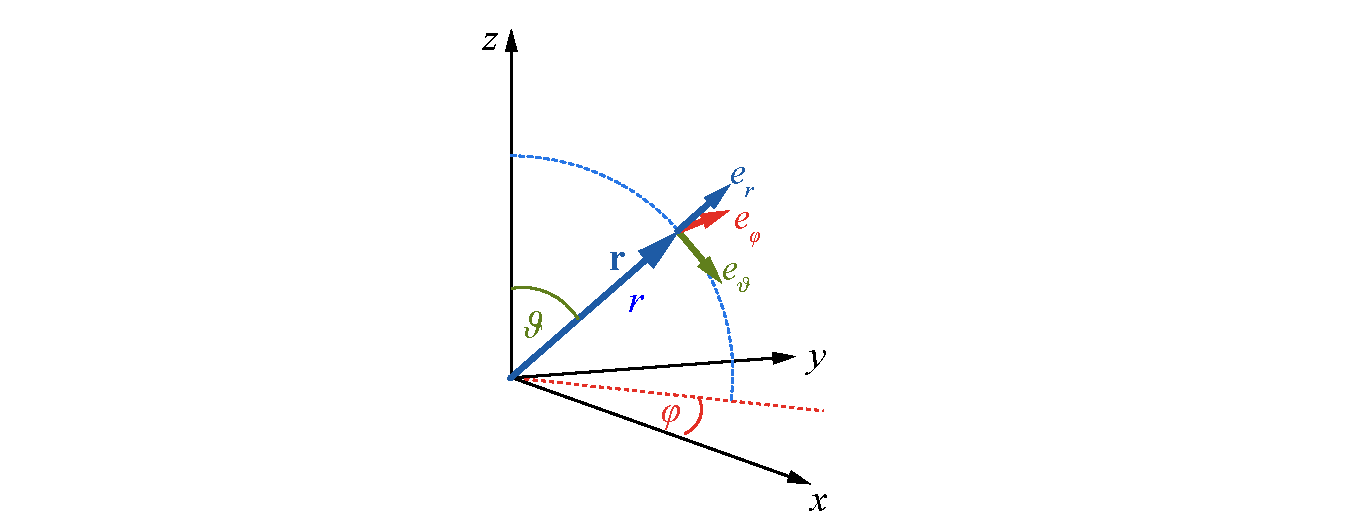
\includegraphics[width=\textwidth]{UebungKOS.pdf}%
\caption{Zur Herleitung der Beschleunigung in Kugelkoordinaten}
\label{abb:lsg_Uebung01}
\end{figure}

Die Vektoren $\vec{e}_r, \vec{e}_\vartheta, \vec{e}_\varphi$ bilden hierbei ein Rechtssystem.
Es ist $\vec{r}=r\:\vec{e}_r$ und die differentielle �nderung des Vektors kann man leicht geometrisch ableiten zu
\begin{align}
\D\vec{r} = \D r\:\vec{e}_r + r\,\D\vartheta\:\vec{e}_\vartheta + r\sin\vartheta \,\D\varphi\:\vec{e}_\varphi ~. \label{eq:lsg_bew_KOS_Formel1}
\end{align}
Daraus folgt 
\begin{align}
\vec{v} = \frac {\D\vec{r}}{\D t} = \dot{r}\:\vec{e}_r+r\dot{\vartheta}\:\vec{e}_\vartheta+r\sin\vartheta\:\dot{\varphi}\:\vec{e_\varphi} ~. \label{eq:lsg_bew_KOS_Formel2}
\end{align}
W�hrend sich $\vec{v}$ unmittelbar aus $\D\vec{r}$ ergibt, ist $\vec{a} = \dot{\vec{v}} = \ddot{\vec{r}}$ deutlich komplizierter, weil die Einheitsvektoren $\vec{e}_r, \vec{e}_\vartheta, \vec{e}_\varphi$ von $\vec{r}$ und damit von t abh�ngen.
Wir finden:
\begin{align}
\vec{a} = \dot{\vec{v}} = \ddot{r}\:\vec{e}_r + \dot{r}\:\dot{\vec{e}}_r + \dot{r}\,\dot{\vartheta}\:\vec{e}_\vartheta + r\,\ddot{\vartheta}\:\vec{e}_\vartheta + r\,\dot{\vartheta}\:\dot{\vec{e}}_\vartheta + \dot{r} \sin\vartheta\:\dot{\varphi}\:\vec{e}_\varphi \ldots \nonumber \\
+ \: r\,\dot{\vartheta}\:\cos\vartheta\:\dot{\varphi}\:\vec{e}_\varphi+ r\sin\vartheta\:\ddot{\varphi}\:\vec{e}_\varphi + r\sin\vartheta\:\dot{\varphi}\:\dot{\vec{e}}_\varphi \,. \label{eq:lsg_bew_KOS_Formel3}
\end{align}
Die zeitlichen Ableitungen der Einheitsvektoren berechnen sich nach
\begin{align*}
\dot{\vec{e}}_r &= \frac{\D}{\D t} \frac{\vec{r}}{r} = \frac{\vec{v}r-\vec{r}\dot{r}}{r^2} = \killA{\frac{\dot{r}}{r}\:\vec{e}_r} + \dot{\vartheta}\:\vec{e}_\vartheta + \sin\vartheta\:\dot{\varphi}\:\vec{e}_\varphi - \killA{\frac{\dot{r}}{r}\:\vec{e}_r} \,, \\
\dot{\vec{e}}_\varphi &= \frac{\D}{\D t} \frac{\vec{e}_z \times \vec{e}_r}{\sin\vartheta} = \frac{\vecez\times\dot{\vec{e}}_r\:\sin\vartheta - \vecez \times \vec{e}_r \:\dot{\vartheta}\,\cos\vartheta}{\sin^2\vartheta}\\
&= \frac{\vecez\times(\dot{\vartheta}\:\vec{e}_\vartheta + \sin\vartheta\;\dot{\varphi}\:\vec{e}_\varphi)}{\sin\vartheta} - \vec{e}_\varphi\frac{\dot{\vartheta}\cos\vartheta}{\sin\vartheta} = \killA{\vec{e_\varphi}\frac{\dot{\vartheta}\cos\vartheta}{\sin\vartheta}} + \dot{\varphi}\:\vecez \times \vec{e}_\varphi - \killA{\vec{e_\varphi}\frac{\dot{\vartheta}\cos\vartheta}{\sin\vartheta}} \\
&= \dot{\varphi} \lk -\sin\vartheta\:\vec{e}_r - \cos\vartheta\:\vec{e}_\vartheta \rk = - \sin\vartheta\,\dot{\varphi}\:\vec{e}_r - \cos\vartheta\,\dot{\varphi}\:\vec{e}_\vartheta ~~ \text{bzw.} \\
\dot{\vec{e}}_\vartheta &= \frac{\D}{\D t}(\vec{e}_\varphi\times\vec{e}_r) = \dot{\vec{e}}_\varphi \times \vec{e}_r + \vec{e}_\varphi \times \dot{\vec{e}}_r = -\cos\vartheta\,\dot{\varphi}\:\vec{e}_\vartheta \times \vec{e}_r + \dot{\vartheta}\:\vec{e}_\varphi \times \vec{e}_\vartheta \nonumber = \cos\vartheta\,\dot{\varphi}\:\vec{e}_\varphi - \dot{\vartheta}\:\vec{e}_r \,.
\end{align*}
Dann ergibt sich aus \eqref{eq:lsg_bew_KOS_Formel3} f�r die Beschleunigung $\vec{a}$ der etwas un�bersichtliche Ausdruck:
\begin{align}
\vec{a} &= \lk \ddot{r} - r\dot{\vartheta^2} - r\sin^2\vartheta\,\dot{\varphi^2} \rk \:\vec{e}_r + \lk \dot{r}\,\dot{\vartheta} + \dot{r}\,\dot{\vartheta} + r\,\ddot{\vartheta} - r\sin\vartheta\cos\vartheta\dot{\varphi^2} \rk \:\vec{e}_\vartheta \ldots \nonumber \\
&+ \lk \dot{r}\sin\vartheta\,\dot{\varphi} + r\,\dot{\vartheta}\,\cos\vartheta\,\dot{\varphi} + \dot{r}\,\sin\vartheta\,\dot{\varphi} + r\,\dot{\vartheta}\,\cos\vartheta\,\dot{\varphi} + r\,\sin\vartheta\,\ddot{\varphi} \rk \:\vec{e}_\varphi \nonumber \\
&= \lk \ddot{r} - r\,\dot{\vartheta^2} - r\,\sin^2\vartheta\,\dot{\varphi^2})\:\vec{e}_r + (2\dot{r}\,\dot{\vartheta} + r\,\ddot{\vartheta} - r\,\sin\vartheta\,\cos\vartheta\,\dot{\varphi^2} \rk \:\vec{e}_\vartheta \ldots \nonumber \\
&+ \lk 2\dot{r}\,\sin\vartheta\,\dot{\varphi} + 2r\,\cos\vartheta\,\dot{\vartheta}\,\dot{\varphi} + r\,\sin\vartheta\,\ddot{\varphi} \rk \:\vec{e}_\varphi \,.\label{eq:lsg_bew_KOS_Formel4}
\end{align}
Um diesen Ausdruck zu interpretieren, teilen wir die Beschleunigung in drei Komponenten auf: die Parallelbeschleunigung $\vec{a}_\text{P}$ (entlang von $\vec{r}$), die den Betrag der Geschwindigkeit erh�ht, die Zentripetalbeschleunigung $\vec{a}_\text{Z}$ und die Coriolis-Beschleunigung $\vec{a}_\text{Cor}$:
\begin{align}
\vec{a}_\text{P} &=  \ddot{r}\,\vec{e}_r + r\,\ddot{\vartheta}\,\vec{e}_\vartheta + r\,\ddot{\varphi}\,\sin\vartheta\:\vec{e}_\varphi \nonumber \\
\vec{a}_\text{Z} &=  -\lk \dot{\vartheta}^2 + \dot{\varphi^2}\,\sin^2\vartheta\rk \,\vec{e}_r - r\,\dot{\varphi^2}\,\sin\vartheta\,\cos\vartheta \,\vec{e}_\vartheta \nonumber \\
\vec{a}_\text{Cor} &=  2\,\dot{r}\,\dot{\vartheta}\:\vec{e}_\vartheta + 2 \lk r\,\sin\vartheta \:+ \:r\,\dot{\vartheta}\,\cos\vartheta \rk \dot{\varphi}\,\vec{e}_\varphi\,.\label{eq:lsg_bew_KOS_Formel5}
\end{align}
\end{sol} 

%\href{PhysikUncut_Part1.pdf#prb:bew_KOS_Formel}{\textcolor{blue} {$\rightarrow$ zur \probref{bew_KOS_Formel}.}}\\
\textcolor{blue} {$\rightarrow$ zur} \probref{bew_KOS_Formel}.\\
\noindent\rule[1ex]{\textwidth}{0.5pt}  \newpage  \clearpage

%-----------------------------------------------------------------------------------------------------------

\hypertarget{lsg:bew_konserv_Kraft}{}
\begin{sol}{prob:bew_konserv_Kraft}\label{lsg:bew_konserv_Kraft} %�bung2
\textbf{Konservatives Kraftfeld} \\ \\
Nach Voraussetzung ist $\vec{F}=\vec{F}(\vec{r})$.
\begin{subprobs}
\subprob{Beweis, dass $\vec{F}$ konservativ ist.}
Die Arbeit berechnet sich nach: 
\begin{align*}
W = -\int{}{}\vec{F}(\vec{r})\,\D r~,
\end{align*}
bzw. differentiell geschrieben: 
\begin{align}
\D W = \frac{\d W}{\d \vec{r}} \,\D \vec{r} + \underbrace{\frac{\d W}{\d \dot{\vec{r}}} \,\d \dot{\vec{r}} + \frac{\d W}{\d t} \,\d t}_{0} ~, \label{eq:lsg_bew_konserv_Kraft1}
\end{align}
da die Kraft nur von $\vec{r}$ abh�ngig ist.
Andererseits ist die differentielle Arbeit definiert durch $\delta W= -\vec{F} \:\D\vec{r} $, woraus $\D W = \delta W$ folgt und somit
\begin{align}
\vec{F} = - \frac{\d W}{\d \vec{r}} = -\gradv \cdot W ~. \label{eq:lsg_bew_konserv_Kraft3}
\end{align}
Das entspricht genau der Definition eines konservativen Kraftfeldes.\textqed \\
%
\subprob{Beweis, dass $\vec{rot}\,\vec{F}  = 0$.}
Da $\vec{F} = -\gradv \: W$, kann man schreiben: 
\begin{align*}
\rotv \vec{F}= - \rotv \times \gradv \:W \,.
\end{align*}
Unter der Voraussetzung der Vertauschbarkeit zweiter Ableitungen, also
\begin{align*}
\frac{\d^2}{\d x_i \d x_j} = \frac{\d^2}{\d x_j \d x_i}~,
\end{align*}
kann man mit Vektoralgebra leicht zeigen, dass
\begin{align*} 
\curl \vec{F} &= \lk -\frac{\d^2}{\d y\d z} + \frac{\d^2}{\d z\d y} \rk F \,\veceX  + \lk-\frac{\d^2}{\d z\d x} + \frac{\d^2}{\d x\d z} \rk F \,\veceY + \lk -\frac{\d^2}{\d x\d y} + \frac{\d^2}{\d y\d x} \rk F \,\veceZ\\
 &= 0 \,. 
\end{align*}
Daher gilt allgemein: 
\begin{align*}
\rotv \gradv U(\vec{r}) = \rotv \gradv \,U = 0 \,. \mmqed
\end{align*}
%
\newpage
\subprob{Beweis, dass $W= -\int\vec{F}\,\D\vec{r}$ nicht vom Weg abh�ngt.}
Wir betrachten zwei Wege $S_1$ und $S_2$, die die gleichen Endpunkte haben.
Aus \eqref{eq:lsg_bew_konserv_Kraft3} folgt allgemein: 
\begin{align}
W_{S_1} = -\int\limits_{S_1} \vec{F}\,\D\vec{r} = \int\limits_{S_1} \gradv U\D\vec{r} = U(\vec{r_2}) - U(\vec{r_1}) ~. \label{eq:lsg_bew_konserv_Kraft5}
\end{align}
Analog folgt:         
\begin{align}
W_{S_2} = -\int\limits_{S_2} \vec{F}\,\D\vec{r} = \int\limits_{S_2} \gradv U\D\vec{r} = U(\vec{r_2}) - U(\vec{r_1}) ~. \label{eq:lsg_bew_konserv_Kraft6}
\end{align}
In beiden F�llen h�ngt die Arbeit also nur von der Potentialdifferenz zwischen Start- und Endpunkt ab und nicht von dem dazwischen liegenden Weg. 

\subprob{Beweis, dass $\oint\limits_{S} \vec{F} \,\D\vec{r} = 0$.}
Wir schreiben f�r die geschlossene Kurve $S = S_1 - S_2$.
Dann folgt mit den Zusammenh�ngen aus der vorigen Teilaufgabe \eqref{eq:lsg_bew_konserv_Kraft5} und \eqref{eq:lsg_bew_konserv_Kraft6} sofort:
\[\oint\limits_{S} \vec{F} \, \D\vec{r} = W_{S_1} - W_{S_2} = 0~. \mmqed \]

\end{subprobs}
\end{sol} 
%\href{PhysikUncut_Part1.pdf#prb:bew_konserv_Kraft}{\textcolor{blue} {$\rightarrow$ zur \probref{bew_konserv_Kraft}.}}\\
\textcolor{blue} {$\rightarrow$ zur} \probref{bew_konserv_Kraft}.\\
\noindent\rule[1ex]{\textwidth}{0.5pt}  \newpage  \clearpage

%-----------------------------------------------------------------------------------------------------------

\hypertarget{lsg:bew_Rot_System}{}
\begin{sol}{prob:bew_Rot_System}\label{lsg:bew_Rot_System}%�bung3
\textbf{Zeitableitung in rotierenden Koordinatensystemen} \\ \\
Wir starten von den Gleichungen f�r die zeitliche Ableitung eines beliebigen Vektors $\vec{A}$ bzw. $\vec{A'}$ in seinem jeweiligen KOS, also beispielsweise
\begin{align*}
	\frac{\D \vec{A'}}{\D t} = \frac{\D A_1'}{\D t} \:\vecpeX + \frac{\D A_2'}{\D t} \:\vecpeY + \frac{\D A_3'}{\D t} \:\vecpeZ \,~.
\end{align*}
Wollen wir die zeitliche Entwicklung im Inertialsystem berechnen, m�ssen wir noch die zeitliche Ableitung der entsprechenden Einheitsvektoren ber�cksichtigen, sodass
\begin{align}
	\frac{\D \vec{A}}{\D t} = \frac{\D \vec{A'}}{\D t} + A_1' \: \dvecepx + A_2' \: \dvecepy + A_3' \: \dvecepz \,.\label{eq:lsg_bew_Rot_System1}
\end{align}
Die Basisvektoren $\vec{e}_i$ sind im Inertialsystem fest verankert und daher konstant.
Die Basisvektoren $\vec{e}'_i$ sind fest am rotierenden System und rotieren mit der Winkelgeschwindigkeit $\vec{\omega'}$ um den Ursprung des KOS $\vec{\Sigma}'$.
Die Geschwindigkeit der gestrichenen Basisvektoren ist also
\begin{align}
	\frac{\D \vec{e}'_i(t)}{\D t} = \vec{\omega'} \times \vec{e}'_i(t) \,. \label{eq:lsg_bew_Rot_System2}
\end{align}
F�r $\vec{A}$ k�nnen wir auch den zeitabh�ngigen Ortsvektor $\vec{A}(t) = \vec{r}(t) = \vec{R}(t) + \vec{r'}(t)$ einsetzen, wobei $\vec{R}(t)$ die Verschiebung des Nullpunktes der KOS darstellt.
Mit \eqref{eq:lsg_bew_Rot_System2} kann man die Zeitableitung von $\vec{A}(t)$ berechnen, indem man die rechte Seite von \eqref{eq:lsg_bew_Rot_System1} als Operator auffasst und auf $\vec{R}(t) + \vec{r'}(t)$ anwendet.
Man erh�lt dann sofort \eqref{eq:bew_Rot_System4}.
\end{sol} 
%\href{PhysikUncut_Part1.pdf#prb:bew_Rot_System}{\textcolor{blue} {$\rightarrow$ zur \probref{bew_Rot_System}.}}\\
\textcolor{blue} {$\rightarrow$ zur} \probref{bew_Rot_System}.\\
\noindent\rule[1ex]{\textwidth}{0.5pt}  \newpage  \clearpage


%-----------------------------------------------------------------------------------------------------------
\hypertarget{lsg:bew_SpaceStation}{}
\begin{sol}{prob:bew_SpaceStation}\label{lsg:bew_SpaceStation} %�bung4
\textbf{Moderne Raumstation} \\ \\
Wir wollen annehmen, dass der Astronaut, wenn er im �u�eren Ring arbeitet, die gewohnte Erdbeschleunigung sp�rt, d.h. die Station rotiert mit:
	\begin{align*}
		\omega = \sqrt{\frac{g}{R_\text{S}}}=\sqrt{\frac{2g}{D_\text{S}}}\approx \SI{0.512}{\per\second} \,.
	\end{align*}
Das entspricht einer Umdrehungszeit von $12\,\mathrm{s}$. 
Wir wollen nun die verschiedenen Fragen zu den wirkenden Kr�ften beantworten.
\begin{subprobs}
\subprob{Bewegung entlang des Tubus}
Wir betrachten die Bewegung des Astronauten entlang des Tubus, also im Inertialsystem $\vec{\Sigma}$.
F�r die $\pi R_\text{S}\approx \SI{120}{m}$ wollen wir etwa eine Minute veranschlagen, was einer Geschwindigkeit von $v_\text{A}=\SI{2}{\meter\per\second}$ entspricht. \\
Durch die Bewegung des Astronauten �ndert sich die effektive \anf{Schwerebeschleunigung} auf den Astronauten und zwar je nachdem, in welche Richtung er relativ zur Rotationsrichtung auf die andere Seite gelangen will:
	\begin{align*}
		\text{gleichsinnige Bewegung:} \quad \omega_\text{eff}&=\omega+\frac{v_\text{A}}{R_\text{S}} \quad \Rightarrow \quad g_\text{eff,s}=\omega_\text{eff}^2\, R_\text{S} \approx \SI{12}{\meter\per\second^2} \,, \\
		\text{gegensinnige Bewegung:} \quad \omega_\text{eff}&=\omega-\frac{v_\text{A}}{R_\text{S}} \quad \Rightarrow \quad g_\text{eff,s} \approx \SI{7.9}{\meter\per\second^2}\,.
	\end{align*}
Er sollte sich also besser \anf{gegensinnig} auf die andere Seite der Station begeben.
Bei einer sich gegen den Uhrzeigersinn drehenden Station sollte er also im Uhrzeigersinn laufen.
\subprob{Bewegung entlang des senkrechten Mittelgangs}
Nun will der Astronaut eine Abk�rzung durch den direkten Verl�ngerungsgang w�hlen.
Wir betrachten seine Bewegung jetzt folglich im mitbewegten System $\vec{\Sigma}'$.
Wir betrachten zun�chst die Coriolis-Kraft.
Der Astronaut ($\SI{100}{\kg}$) wird mit dieser gegen die seitliche Wand des Tunnels gedr�ckt.
		\begin{align*}
				\vec{F}_\text{Cor}'= -2m\,\omega \begin{pmatrix}
  0\\ 
  v_\text{A} \\
	0
\end{pmatrix} \approx -200 \,\mathrm{N} \cdot \veceY \,.
		\end{align*}
Wir betrachten noch den Energieaufwand, den der Astronaut in diesen Fall gegen das k�nstliche \anf{Schwerefeld} aufbringen muss.
Beim Gang bis zur Mitte arbeitet er gegen das k�nstliche Schwerefeld, danach k�nnte er die potentielle Energie mit Hilfsmitteln wieder zur�ckgewinnen:
	\begin{align*}
		\Delta E &= \int\limits_{R_\text{S}}^{0} F_\text{z}'\,\D r' = -m\,\omega^2\,r' \,\D r' \,.\\
		&= +\frac{m}{2} \,\omega^2\,{R_\text{S}}^2 \approx \SI{18200}{\newton\meter} \approx 0.005 \,\mathrm{kWh}  \approx 4350 \, \mathrm{cal} \,.
	\end{align*}
Das ist also kein �quivalentes Training f�r den Astronauten, um fit zu bleiben.

\newpage
\subprob{Weitere Schwierigkeit}
Zum Schluss wollen wir noch die Gezeitenkraft, die wir im Detail in der Himmelsmechanik (Kapitel 3 im Teil 2 dieser Reihe) behandeln werden, absch�tzen.
Auf den Astronauten (Gr��e $\SI{2}{\meter}$) wirken ja im k�nstlichen \anf{Schwerefeld} auf seinen Kopf (K) und seine F��e (F) unterschiedlich gro�e Kr�fte.
		\begin{align*}
				F_\text{K} &= m \,g_\text{K} = m \,\omega^2 \,(R_\text{S}-h_\text{A}) \,,\\
				F_\text{F} &= m \,g_\text{F} = m \,\omega^2 \, R_\text{S}\,, \\
				\Delta F &= -m \,\omega^2 h_\text{A} \approx 52 \, \mathrm{N} \,.
		\end{align*}
Das ist ein nicht unerheblicher Kraftunterschied, dessen Wirkung auf den K�rper (Blutfluss, Koordination) sicher nicht zu vernachl�ssigen ist.
Ob sich ein Astronaut auf so einer Station wohlf�hlt bleibt abzuwarten.
Die Bedingungen kann man nat�rlich verbessern, wenn man $R_\text{S}$ gr��er macht.
\end{subprobs}
\end{sol} 
%\href{PhysikUncut_Part1.pdf#prb:bew_SpaceStation}{\textcolor{blue} {$\rightarrow$ zur \probref{bew_SpaceStation}.}}\\
\textcolor{blue} {$\rightarrow$ zur} \probref{bew_SpaceStation}.\\
\noindent\rule[1ex]{\textwidth}{0.5pt}  \newpage  



%-----------------------------------------------------------------------------------------------------------
\hypertarget{lsg:bew_SpaceElevator}{}
\begin{sol}{prob:bew_SpaceElevator}\label{lsg:bew_SpaceElevator} %�bung5
\textbf{Weltraumfahrstuhl}
\begin{subprobs}
	\subprob{Anforderungen an das Seil}  
		Wir betrachten zun�chst einen Satelliten in einer geostation�ren Umlaufbahn, dessen H�he $h_\text{G}$ �ber dem �quator man leicht ausrechnen kann, indem man im mitbewegten System $\vec{\Sigma}'$ fordert, dass die Zentrifugalkraft gleich der Gravitationskraft ist:
		\[ -\frac{G\,m_\text{E}\,m}{R_\text{G}^2} + m\,\omega_\text{E}'^2\,R_\text{G} = 0 \,, ~  R_\text{G} = R_\text{E} + h_\text{G}\, .
		\]
		Hierin sind $R_\text{E}$, $m_\text{E}$ der Radius bzw. die Masse der Erde und $\omega_\text{E}'= {2\pi}/{86125}\,\text{s}^{-1}$ die Rotationsfrequenz der Erde.
		Man erh�lt daraus eine Beziehung f�r $R_G$. Der Einfachheit halber lassen wir die Striche weg, da wir nur im mitbewegten System rechnen:
		\begin{align}
		R_\text{G} = R_\text{E} + h_\text{G} = \sqrt[3]{\frac{G\,m_\text{E}}{\omega_\text{E}^2}} \approx \SI{42000}{km} \, .
		\label{lsg:bew_SpaceElevator_1}
		\end{align}
		
\begin{figure}[H]
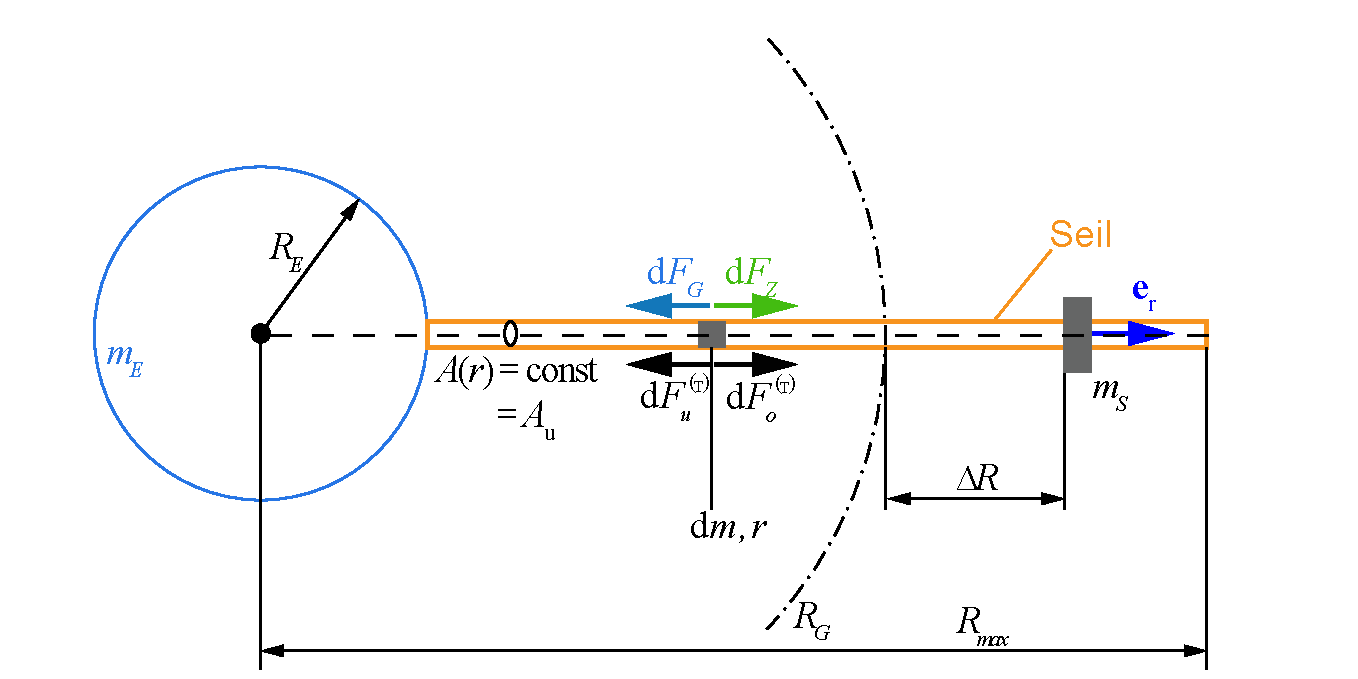
\includegraphics[width=\textwidth]{SpaceElevator_1.pdf}%
\caption{Modell des Weltraumfahrstuhls mit konstanter Seildicke}
\label{abb:lsg_SpaceElevator_1}
\end{figure}
		
	\begin{enumerate} [a) ]
		\item Konstante Seildicke \\
		Wir betrachten nun die \figref{lsg_SpaceElevator_1}.
    Das Seil muss offensichtlich im System $\vec{\Sigma} '$ ruhen. 
		F�r einen beliebigen Massepunkt entlang des Seils gilt dann nach der Zeichnung f�r den Fall eines Seils mit  konstanter Dicke und der Massendichte~$\rho$ und zun�chst einer Endmasse $m_\text{S}=0$ folgende Kr�ftebilanz, wobei die $F_\text{o,u}^{(\text{T})}$ die Seilspannungskr�fte nach oben und unten sind und $\text{d}F_\text{G}$, $\text{d}F_\text{Z}$ die differentielle Schwerkraft bzw. Zentrifugalkraft:
		\begin{align}
		F_\text{o}^{(\text{T})} - F_\text{u}^{(\text{T})} = \D F^{(\text{T})} = A_\text{u}\,\D \sigma^{(\text{T})} = A_\text{u} \,\rho \,\D r \lek  \underbrace{\frac{G \,m_\text{E}}{r^2}}_{\text{d}F_\text{G}} - \underbrace{\omega_\text{E}^2 \,r }_{\D F_\text{Z}}\rek\, .
		\label{lsg:bew_SpaceElevator_2}
		\end{align}
		Die Gr��e $\D \sigma^{(\text{T})}$ ist die differentielle Seilspannung (in \SI{}{\newton\per\meter\squared}) und hat die $r$-Abh�ngigkeit
		\begin{align}
		\frac{\D \sigma^{(\text{T})}(r)}{\D r} = G\, m_\text{E} \,\rho \,\biggl[\frac{1}{r^2} - \frac{r}{R_\text{G}^3}\biggl]\,,
		\label{lsg:bew_SpaceElevator_3}
		\end{align}
		wobei wir \eqref{lsg:bew_SpaceElevator_1} benutzt haben.
		Die Integration von $R_\text{E}$ bis $R_\text{G}$ ergibt die Spannung im Seil bei $r = R_\text{G}$:
		\begin{align}
		\sigma(R_\text{G}) = G \,m_\text{E}\,\rho\:\biggl[ \frac{1}{R_\text{E}} - \frac{3}{2R_\text{G}} + \frac{R_\text{E}^2}{2R_\text{G}^3}\biggl] \, .
		\label{lsg:bew_SpaceElevator_4}
		\end{align}
		Wir wollen nun die notwendige Seill�nge $L_\text{Seil}^{(1)}  = R_ \text{max} - R_\text{E}$ ermitteln. 
		Da das Seil im mitbewegten System ruhen muss, muss f�r alle Massepunkte die resultierende Spannung verschwinden, also mit \eqref{lsg:bew_SpaceElevator_2}:
		\begin{align}
		A_\text{u} \rho  \int_{R_\text{E}}^{R_\text{max}} r \text{d}r \,\biggl[\frac{Gm_\text{E}}{r^3} - \omega_\text{E}^2\biggl] &\overset{!}{=} 0
		\label{lsg:bew_SpaceElevator_5}\\
		\Rightarrow \frac{1}{2} \omega_\text{E}^2\,(R_\text{max}^2 - R_\text{E}^2) &= Gm_\text{E} \,\biggl(\frac{1}{R_\text{E}} - \frac{1}{R_\text{max}} \biggl)\, ,
		\end{align}
		woraus eine quadratische Gleichung f�r $R_ \text{max}$ resultiert\footnote{Eigentlich resultiert eine kubische Gleichung, aber die triviale L�sung $R_\text{max} = R_\text{E}$ kann eliminiert werden.}, deren physikalisch sinnvolle L�sung
		\begin{align}
		R_\text{max} &= \frac{R_\text{E}}{2} \lk\sqrt{1 + \frac{8 G\,m_\text{E}}{\omega_\text{E}^2 \,R_\text{E}^3} } - 1\rk = \frac{R_\text{E}}{2} \lk \sqrt{1 + 8 \lk \frac{R_\text{G}}{R_\text{E}} \rk^3} - 1\rk \:\approx \SI{150000}{km}\, , \nonumber \\
		L_\text{Seil}^{(1)} &= R_\text{max} - R_\text{E} = \frac{R_\text{E}}{2} \,\lk \sqrt{1 + 8 \lk \frac{R_\text{G}}{R_\text{E}} \rk^3} - 3\rk \:\approx \SI{144000}{km}
		\label{lsg:bew_SpaceElevator_6}
		\end{align}
		ist, wobei wir \eqref{lsg:bew_SpaceElevator_1} benutzt haben.

		\item Variabler Querschnitt mit konstanter Seilinnenspannung \\
		 Betrachten wir nun ein Seil, welches einen variablen Durchmesser hat (\figref{lsg_SpaceElevator_2}) und zwar so, dass die Spannung $\sigma_\text{c}$ im Seil �berall gleich gro� ist. 

\begin{figure}[H]
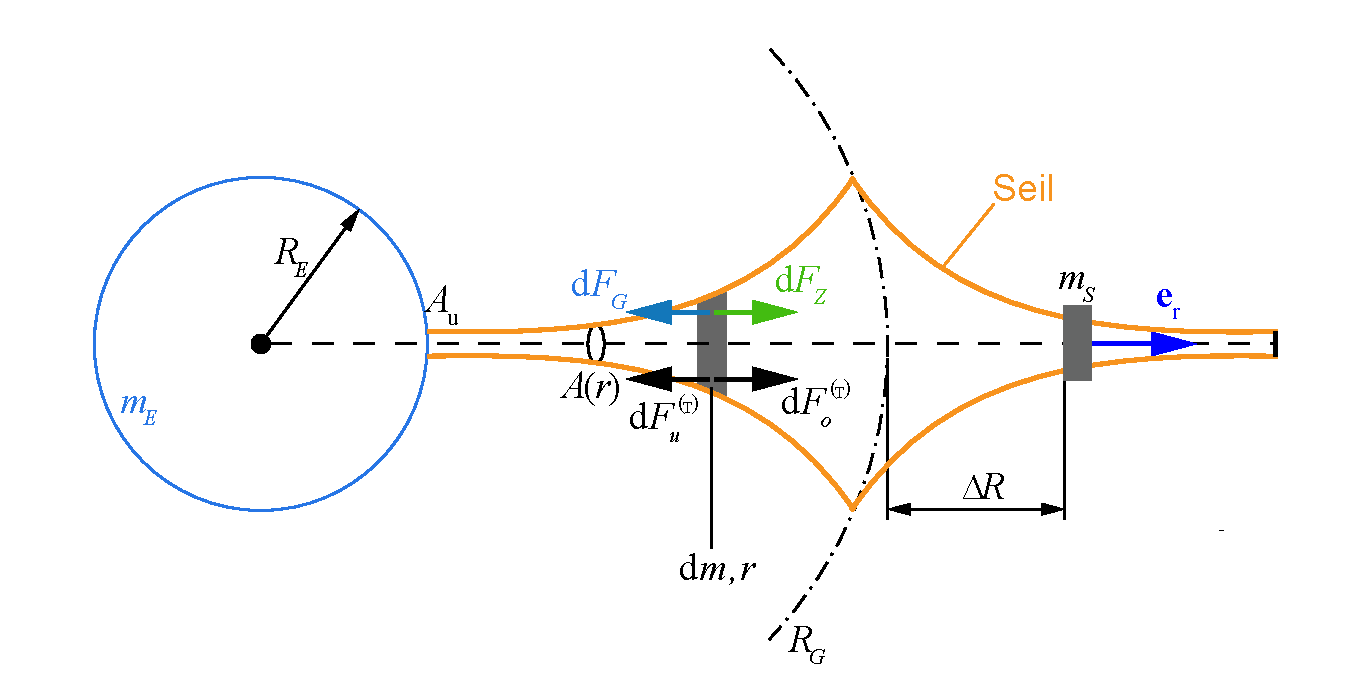
\includegraphics[width=\textwidth]{SpaceElevator_2.pdf}%
\caption[Modell des Weltraumfahrstuhls mit konstanter Seilspannung]{Modell des Weltraumfahrstuhls mit konstanter Seilspannung $\sigma_\text{c}$}
\label{abb:lsg_SpaceElevator_2}
\end{figure}

		Dann muss die Gleichung \eqref{lsg:bew_SpaceElevator_2} lauten:
		\begin{align}
		\D F_\text{o}^{(\text{T})} - \D F_\text{u}^{(\text{T})} = \sigma_\text{c} \, \D A = \rho A(r) \, \lek \frac{G \, m_\text{E}}{r^2} - \omega_\text{E}^2 \, r \rek \, \D r\, , 
		\label{lsg:bew_SpaceElevator_7}
		\end{align}
		bzw. integriert:
		\begin{align}
		A(r) = A_\text{u} \exp \lk \frac{\rho \,g \,R_\text{E}^2}{\sigma_\text{c}} \lek \frac{1}{R_\text{E}} + \frac{R_\text{E}^2}{2R_\text{G}^3} - \frac{1}{r} - \frac{r^2}{2R_\text{G}^3} \rek \rk \, .
		\label{lsg:bew_SpaceElevator_8}
		\end{align}
		Hierbei haben wir $g=\frac{G\,m_\text{E}}{R_\text{E}^2}$ gesetzt und $A(R_\text{E}) = A_\text{u}$.\\
		Die L�nge des Seils, wiederum ohne Gegengewicht ($m_\text{s}=0$), erhalten wir, indem wir fordern, dass $A(R_\text{max}) = A(R_\text{E})$:
		\begin{align}
		\Rightarrow L_\text{Seil}^{(2)} = \frac{R_\text{E}}{2} \lek \sqrt{1 + 8\lk\frac{R_\text{G}}{R_\text{E}}\rk^3} -1 \rek - \frac{2R_\text{E}}{2} = \frac{R_\text{E}}{2}\lek \sqrt{1 + 8\lk\frac{R_\text{G}}{R_\text{E}}\rk^3} -3 \rek \, ,
		\label{lsg:bew_SpaceElevator_9}
		\end{align}
		was identisch mit \eqref{lsg:bew_SpaceElevator_6} ist.
	\end{enumerate}

	\subprob{Vergleich und Argumentation zur Machbarkeit} 
	Wir wollen nun die beiden Varianten vergleichen und benutzen dazu Materialparameter von m�glichen Materialien. 
	Im Fall a) mit konstanter Seildicke m�ssen wir uns also offensichtliche Gedanken �ber die  maximal auftretende (Zug-)Spannung im Seil $\sigma_\text{max} = \sigma(R_\text{G})$ machen. 
	Bei Fall b) mit konstanter (max. zul�ssiger) Zugspannung $\sigma$ hingegen sollte eher die maximale Seildicke bzw. den Seilquerschnitt $A_\text{max} = A(R_\text{G}) = \frac{\pi}{4}d_\text{max}^2$ in Betracht gezogen werden.\\
	% (d_u = \SI{5}{\milli\meter}) % was ist das? wozu diese Angabe?
	\begin{table}[h!]
		\centering
		\caption[Berechnungen f�r Weltraumfahrstuhl auf der Erde.]{Berechnungen f�r Weltraumfahrstuhl auf der Erde f�r Fall a (Seil mit $A=\text{const}$) und Fall b (Seil mit $\sigma=\text{const}$) und verschiedene Materialien. (Mit Taper Ratio wird das Verh�ltnis von Maximal- zu Minimalseilquerschnitt bezeichnet.)}
		\begin{tabular}{lccccc}
			Material& Zugfestigkeit	& Dichte & Fall a	& Fall b &Taper Ratio\\
			&$\quad \sigma_\text{mat} \left[\SI{}{GPa}=\SI{}{\newton\per\meter\squared}\right]\quad $ & $\quad \rho \left[\frac{\text{kg}}{\text{m}^3}\right]\quad $ &$\quad \sigma_\text{max} \left[\SI{}{GPa}\right]\quad $			& $\quad d_\text{max} \left[\SI{}{\milli\meter}\right]\quad $&\\
			\midrule
			Karbon	& $\approx 100$ & $1300$ &  63	& $7 $& 1.9\\
			Kevlar	& $\approx 4 $ & $1440$ &  70	&	$3\, 10^{02}$& 3100	\\
			Dyneema	& $\approx 3 $ & $ 970$ &  44	&	$7\, 10^{01}$& 720	\\
			Stahl 	& $\approx 5 $ & $7900$ & 383	&	$2\, 10^{13}$& $2\, 10^{16}$	\\
		\end{tabular}
	\end{table}

	Man erkennt, dass es, wenn es �berhaupt eine machbare L�sung geben kann, diese nur mit Karbonfasern realisierbar w�re.
        In diesem Fall w�rde das Seil im g�nstigsten Fall $\SI{7}{\mm}$ dick sein.
	Insgesamt scheint die Realisierungschance beim Seil mit variablem Querschnitt gr��er.
        Aber selbst dann gibt es offene Fragen:
	\begin{itemize}
		\item Haltbarkeit
		\item Rei�en durch Einfluss von \anf{Space Debris} (Raumfahrtm�ll)
		\item Materialerm�dung �ber die Zeit u.v.a.m.
		\item Coriolis-Kraft: Wir haben bisher noch nicht ber�cksichtigt, dass sich eine Nutzlast mit einer bestimmten Geschwindigkeit entlang des Seils nach oben bewegen muss.
                  Wie wir im Kapitel \ref{kap:bew_Coriolis-Kraft} gesehen haben, f�hrt eine Bewegung senkrecht nach oben im rotierenden Bezugssystem zu einer seitlichen Ablenkung.
                  Das Seil w�rde also anfangen seitw�rts zu schwingen.
                  Der Leser kann mit Gleichung \eqref{eq:bew_Coriolis_Kraft} selbst absch�tzen, wie gro� die Kraft ist bzw. wie langsam sich der Fahrstuhl bewegen m�sste, damit die seitliche Kraft klein gegen�ber der Querspannung im Material bleibt.
	\end{itemize}
\subprob{Vorteile durch Anbringen eines Gegengewichts}
	Wir wollen nun noch untersuchen, ob sich die Rahmenbedingungen verbessern lassen, wenn man an geeigneter Stelle im Abstand $\Delta R$ von $R_\text{G}$ ein Gegengewicht der Masse $m_\text{c}$ anbringt.
        Dann muss dort folgende Kr�ftebilanz erf�llt sein:
	\begin{align}
	F_\text{G}^{(m_\text{S})} + F^{(\text{T})} &= F_\text{z}^{(m_\text{S})} \, ,\\
	\frac{G\, m_\text{E}\, m_\text{S}}{\left[R_\text{G}+\Delta R\right]^2} + A(R_\text{G} + \Delta R)\, \sigma &= m_\text{S}\, \omega_\text{E}^2\,\left[ R_\text{G}+\Delta R \right] \, .
	\label{lsg:bew_SpaceElevator_10}
	\end{align}
	Wir nutzen die Beziehung \eqref{lsg:bew_SpaceElevator_8} f�r $A(R_\text{G}+\Delta R)$ und erhalten f�r die Masse $m_\text{S}$ als Funktion der Position $\Delta R$:
	\begin{align}
	m_\text{S}(\Delta R) &= \frac{A_\text{u} \, \sigma_\text{mat}}{g} \frac{\mathrm{e} \lek[\frac{R_\text{E}^2\, \rho \, g}{2\sigma \, R_\text{G}^3} \lk\frac{2R_\text{G}^3 + R_\text{E}^3}{R_\text{E}} - \frac{2R_\text{G}^3 + (R_\text{G}+\Delta R)^3}{R_\text{G} + \Delta R}\rk\rek}{\frac{R_\text{E}^2\, (R_\text{G} + \Delta R)}{R_\text{G}^3}\lek 1 - \lk\frac{R_\text{G}}{R_\text{G} + \Delta R}\rk^3\rek} \,. 	\label{lsg:bew_SpaceElevator_11}
	\end{align}
	Man kann leicht sehen, dass $m_\text{S} \rightarrow \infty$, wenn $\Delta R \rightarrow 0$, also muss die Masse au�erhalb der geostation�ren Bahn liegen.
        Man kann also die L�nge des Seils ver�ndern, wenn man die Zusatzmasse $m_\text{S}$ anbringt.
        Die Gesamtmasse ist dann 
	\begin{align}
	m_\text{tot}(\Delta R) &= m_\text{S} + m_\text{Seil} = m_\text{S} + \rho \int\limits_{R_\text{E}}^{R_\text{G} + \Delta R} A(r) \, \D r \, .
	\label{lsg:bew_SpaceElevator_12}
	\end{align}
	Das Integral in Gleichung \eqref{lsg:bew_SpaceElevator_12} berechnen wir numerisch.
        In \figref{lsg_SpaceElevator_3} sind f�r die unterschiedlichen Materialparameter die Massen $m_\text{S}, ~ m_\text{Seil}$ als Funktion der Position $\Delta R$ gezeigt.
\begin{figure}[H]
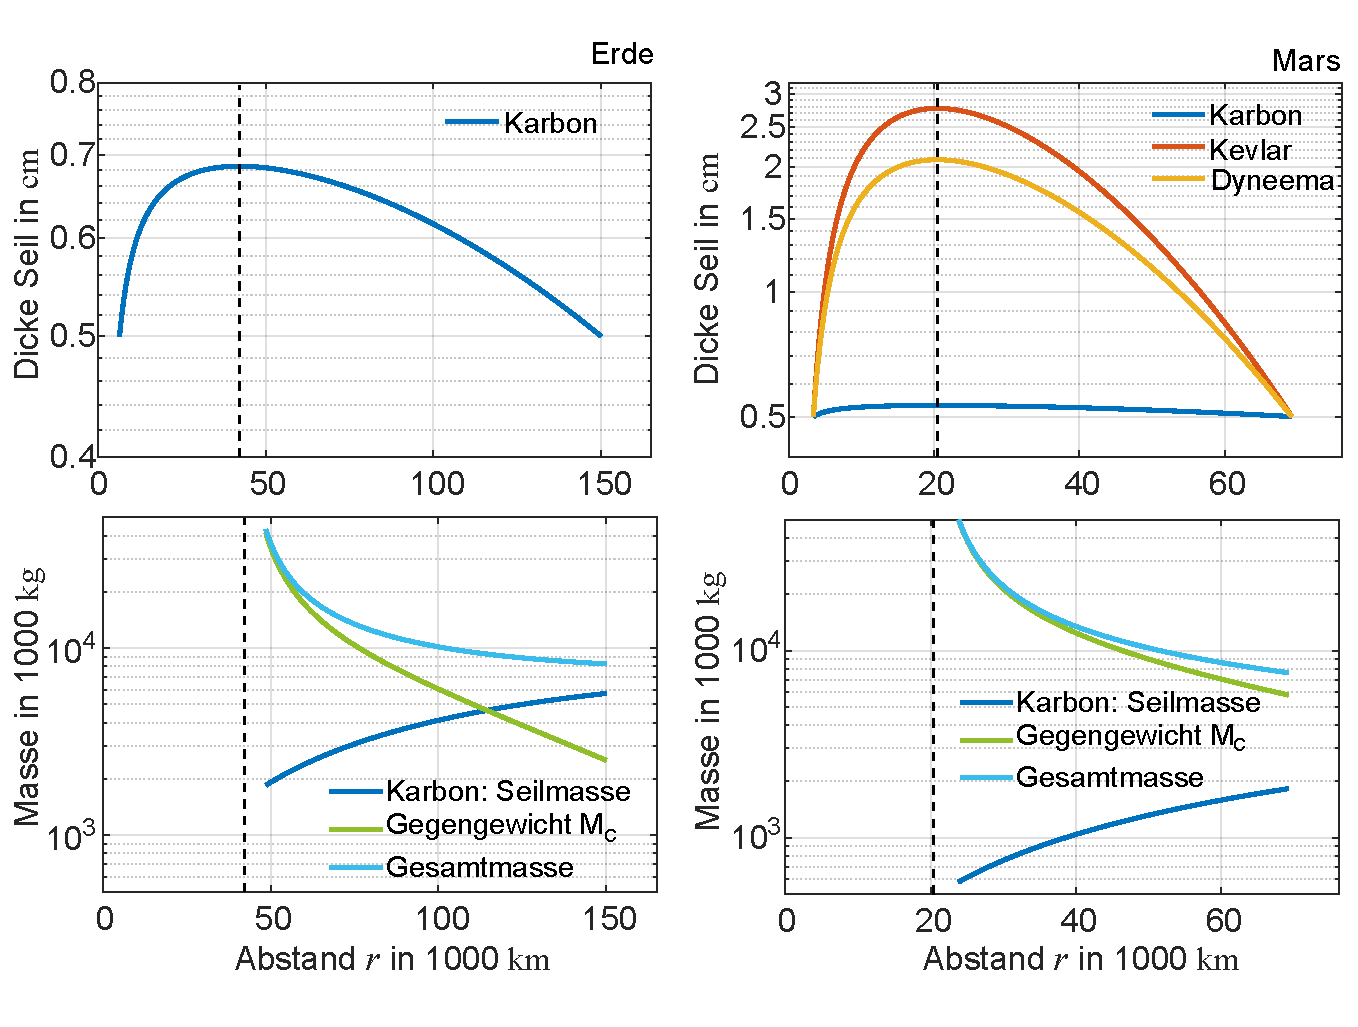
\includegraphics[width=\textwidth]{SpaceElevator_3.pdf}%
\caption[Seilmassen und Zusatzmasse]{Seilmassen und Zusatzmasse als Funktion der Position der Zusatzmasse f�r verschiedene Materialparameter}
\label{abb:lsg_SpaceElevator_3}
\end{figure}

\subprob{(Energetischer) Nutzen des Space Elevators} 
	Wir wollen nun die Energie berechnen, die mit dem Space Elevator gespart werden kann, wenn man eine Nutzmasse $m_\text{N}$ auf eine bestimmte Bahnh�he $H_\text{B} = r_\text{B} - R_\text{E}$ zu bringen hat.
	Beim Fahrstuhl muss man nur die potentielle Energie aufbringen:
	\[ W^{(1)} = \Delta E_\text{pot} = \int\limits_{R_\text{E}}^{H_\text{B}} \frac{G\,m_\text{N} m_\text{E}}{r^2} \D r = -\frac{G m_\text{N} m_\text{E}}{r}\bigg|_{R_\text{E}}^{H_\text{B}+R_\text{E}}\, .
	\]
	Bei einem Raketenstart ist die aufgewendete Arbeit, um eine Nutzlast auf $H_\text{G} = R_\text{G} - R_\text{E}$ zu bringen:
	\begin{align*}
	W^{(2)} &= \Delta E_\text{kin} + \Delta E_\text{pot} = \frac{m_\text{N}}{2}\,  \omega_\text{E}^2 \, R_\text{G}^2 + \Delta E_\text{pot}\,,
\end{align*}
woraus
	\begin{align}
\frac{\Delta W}{W^{(2)}} &= \frac{W^{(1)} - W^{(2)}}{W^{(2)}} = \frac{W^{(1)}}{W^{(2)}} - 1 \approx 8 \% 
	\end{align}
folgt. Wir haben hier nur die Arbeit f�r die Nutzlasten vergleichen.
        Beim Raketenstart m�sste man ja korrekterweise noch den Aufwand, der f�r den Transport des Treibstoffs notwendig ist, ber�cksichtigen (siehe Kapitel 4, Band II).
\subprob{Space Elevator zum Mars}
	F�r den Mars k�nnen wir die Gleichung verwenden und ersetzen
	\begin{align*}
	R_\text{E} &\rightarrow R_\text{M} = \SI{3791}{km} \, , \\
	m_\text{E} &\rightarrow m_\text{M} = \SI{6.417e23}{kg}\, ,\\
	\omega_\text{E} &\rightarrow \omega_\text{M} = \frac{2 \pi}{ 88620 \,\text{s}} = \SI{7.09e-5}{per\second} \,.
	\end{align*}
	Damit ergeben sich mit den gleichen Materialien f�r die Erde folgende Bedingungen f�r einen Weltraumfahrstuhl auf dem Mars.
        Die Realisierungsbedingungen f�r einen solchen Fahrstuhl auf dem Mars sind auf Grund dessen geringerer Masse also deutlich besser, abgesehen nat�rlich von dem logistischen Aufwand.
        Wir �berlassen dem Leser die Absch�tzung f�r den Mond (Man beachte dabei die notwendige L�nge des Seils.) und auch Investitionsentscheidung!
        F�r weitergehende Berechnungen empfehlen wir \cite{Aravind2007, Pearson2005}.\\
	% (d_u = \SI{5}{\milli\meter})
	\begin{table}[H]
		\centering
		\caption[Berechnungen f�r Weltraumfahrstuhl auf dem Mars.]{Berechnungen f�r Weltraumfahrstuhl auf dem Mars f�r Fall a (Seil mit $A=\text{const}$) und Fall b (Seil mit $\sigma=\text{const}$) und verschiedene Materialien.}
		\begin{tabular}{lccccc}
			% \toprule
			Material& Zugfestigkeit	& Dichte 	& Fall a	& Fall b\\
			&$ \quad \sigma_\text{mat} \left[\SI{}{GPa}=\SI{}{\newton\per\meter\squared}\right] \quad $
			& $ \quad \rho \left[\frac{\text{kg}}{\text{m}^3}\right] \quad $ 
			&$ \quad \sigma_\text{max} \left[\SI{}{GPa}\right] \quad $			
			& $ \quad d_\text{max} \left[\SI{}{\centi\meter}\right]  \quad $
			&Taper Ratio\\
			\midrule
			Karbon	& $\approx 100$ & $1300$ & 12	& $0.5$&1\\
			Kevlar	& $\approx 4 $  & $1440$ & 14 &	$2.8$&37	\\
			Dyneema	& $\approx 3 $  & $ 970$ & 9 &	$2.1$&21	\\
			Stahl 	& $\approx 5 $  & $7900$ & 75	&	$920$&$3.4\cdot10^6$\\
			% \bottomrule
		\end{tabular}
	\end{table}
\end{subprobs}
\end{sol} 
%\href{PhysikUncut_Part1.pdf#prb:bew_SpaceElevator}{\textcolor{blue} {$\rightarrow$ zur \probref{bew_SpaceElevator}.}}\\
\textcolor{blue} {$\rightarrow$ zur} \probref{bew_SpaceElevator}.\\
\noindent\rule[1ex]{\textwidth}{0.5pt}  \newpage


%-----------------------------------------------------------------------------------------------------------
\hypertarget{lsg:bew_SkyDiver}{}
\begin{sol}{prob:bew_SkyDiver}\label{lsg:bew_SkyDiver} %�bung6
\textbf{Skydiver} \\ \\

Die numerische Berechnung findet sich in \mlbewref{Skydiver.m}.

\end{sol} 
%\href{PhysikUncut_Part1.pdf#prb:bew_SkyDiver}{\textcolor{blue} {$\rightarrow$ zur \probref{bew_SkyDiver}.}}\\
\textcolor{blue} {$\rightarrow$ zur} \probref{bew_SkyDiver}.\\
\noindent\rule[1ex]{\textwidth}{0.5pt}  \newpage

%-----------------------------------------------------------------------------------------------------------
\hypertarget{lsg:bew_Quizfrage}{}
\begin{sol}{prob:bew_Quizfrage}\label{lsg:bew_Quizfrage} %�bung7
\textbf{Quizfrage} \\ \\

Die numerische Berechnung findet sich in \mlbewref{WurfmitohneReibung.m}.\\
Als Ergebnis ergibt sich: Im Falle mit Reibung ist die Kanonenkugel immer schneller wieder unten. Eng verwandt damit ist die folgende Frage: Braucht in einem Medium mit Reibung die Kugel im Aufstieg oder im Abstieg mehr Zeit, oder sind die Zeiten gleich lang wie im Fall ohne Reibung? Man kann das sich auch ohne numerische Rechnung leicht �berlegen.\\

(�bung nach einer Anregung durch Ref. \cite{Mungan2021}. 

\end{sol} 
%\href{PhysikUncut_Part1.pdf#prb:bew_Quizfrage}{\textcolor{blue} {$\rightarrow$ zur \probref{bew_Quizfrage}.}}\\
\textcolor{blue} {$\rightarrow$ zur} \probref{bew_Quizfrage}.\\
\noindent\rule[1ex]{\textwidth}{0.5pt}  \newpage

%-----------------------------------------------------------------------------------------------------------
\hypertarget{lsg:bew_VielteilchenI}{}
\begin{sol}{prob:bew_VielteilchenI}\label{lsg:bew_VielteilchenI}%�bung8
\textbf{Vielteilchensysteme} \\ \\
Wir wollen die G�ltigkeit folgender Erhaltungss�tze f�r Vielteilchensysteme zeigen.
\begin{subprobs}
\subprob{Impulserhaltung}
Aus \eqref{eq:bew_Gesamtgroessen} folgt mit 
$M = \sum\limits_{i} m_i$ und $\vec{R}= \frac{1}{M} \sum\limits_{i} m_i \, \vec{r}_i$, dass 
\begin{align*}
	&\sum\limits_{i} m_i \, \ddot{\vec{r}}_i = M  \, \ddot{\vec{R}} = \sum\limits_{i} \vec{F}_i^{\text{(ext)}} \\
	\Rightarrow	\quad &\vec{P} = \sum\limits_{i} m_i \, \dot{\vec{r}}_i = M \, \dot{\vec{R}} \,.
\end{align*}
Ist die Summe der �u�eren Kr�fte 0, so ist $M \, \ddot{\vec{R}}= 0$ und damit $\vec{P}=M \, \dot{\vec{R}}=\text{const} $.
D.h. der Gesamtimpuls bleibt erhalten.

\subprob{Drehimpulserhaltung}
Analog kann man zeigen:
\begin{align*}
	\vec{L} &= \sum\limits_{i} \vec{L}_i = \sum\limits_{i} m_i  \, \vec{r}_i\times\dot{\vec{r}}_i \,, \\
	\dot{\vec{L}} &= \underbrace{\sum\limits_{i}m_{i}\dot{\vec{r}}_i\times\dot{\vec{r}}_i}_{\substack{=0}} +\sum\limits_{i} m_i\vec{r}_i\times\ddot{\vec{r}}_i \\
  &= \sum\limits_{i}\vec{r}_i\times\sum\limits_{j}\vec{F}_{ij} +\sum\limits_{i}\vec{r}_i\times{\vec{F}_i}^\text{(ext)} \\
	&= \frac{1}{2}\sum\limits_{i,j}(\vec{r}_i\times\vec{F}_{ij}-\vec{r}_i\times\vec{F}_{ji})+\sum\limits_{i}\vec{r}_i\times{\vec{F}_i}^\text{(ext)} \\
	&= \frac{1}{2}\sum\limits_{i,j}(\vec{r}_i-\vec{r}_j)\times{\vec{F}_{ij}}+\sum\limits_{i}\vec{r}_i\times{\vec{F}_i}^\text{(ext)}~.
\end{align*}
Hierin verschwindet der erste Term, da bei Zentralkr�ften $\vec{F}_{ij} \| (\vec{r}_i-\vec{r}_j)$ gilt.
Folglich ergibt sich die zeitliche �nderung des Gesamtdrehimpulses zu
\[ \dot{\vec{L}}= \sum\limits_{i} \lk \vec{r}_i\times{\vec{F}_i}^\text{(ext)} \rk \,. \]
Wir bezeichnen den Summanden $\vec{r}_i\times{\vec{F}_i}^\text{(ext)}$ als Drehmoment der �u�eren Kraft.
Verschwindet dieses, dann ist $\vec{L}=\vec{const}$.

\end{subprobs}
\end{sol} 
%\href{PhysikUncut_Part1.pdf#prb:bew_VielteilchenI}{\textcolor{blue} {$\rightarrow$ zur \probref{bew_VielteilchenI}.}}\\
\textcolor{blue} {$\rightarrow$ zur} \probref{bew_VielteilchenI}.\\
\noindent\rule[1ex]{\textwidth}{0.5pt}  \newpage

%-----------------------------------------------------------------------------------------------------------
\hypertarget{lsg:bew_SwingBy}{}
\begin{sol}{prob:bew_SwingBy}\label{lsg:bew_SwingBy} %�bung9
\textbf{Swing-By-Man�ver in der Raumfahrt}
\begin{subprobs}
\subprob{Beziehung f�r den Energie�bertrag beim elastischer Sto�}\\
Im System $\vec{\Sigma}'=\Sigma_\text{S}$ sind nach \eqref{eq:bew_Streuung1a} und \eqref{eq:bew_Streuung2a} die Betr�ge der Geschwindigkeiten der beiden wechselwirkenden Teilchen (mit den Massen $m_1,\, m_2$, der Gesamtmasse $M = m_1+m_2$) vor und nach dem Sto� identisch, also:
		\begin{align}
				|\vec{v}_1'| = |\vec{u}_1'| \qquad \text{und} \qquad |\vec{v}_2'| = |\vec{u}_2'| \,. \label{eq:bew_lsg_SwingBy00}
		\end{align}
Damit sind auch die kinetischen Energien gleich.
Im Laborsystem $\vec{\Sigma}_\text{L}$ gilt das nicht mehr, da kommt es zu einem Energie�bertrag.
Wir betrachten den Fall, dass $\vec{v}_2=0$, d.h. der K�rper mit der Masse $m_2$ im Laborsystem ruht.
Dann gilt mit der Schwerpunktgeschwindigkeit nach \eqref{eq:bew_Streuung4}:
	\begin{align}
		{\vec{u}_1}^2 &= (\vec{u}_1'+\dot{\vec{X}})^2 = \lk \vec{u}_1' + \frac{m_1}{M}\vec{v}_1 \rk ^2 ~~\text{mit}~~~ \dot{\vec{X}}=\frac{m_1}{M}\vec{v}_1  \nonumber \\ 
		{\vec{u}_1}^2 &= {\vec{u}_1'}^2+\frac{2m_1}{M}\vec{u}_1'\vec{v}_1+\frac{{m_1}^2}{M^2}{\vec{v}_1}^2 \,,  \nonumber \\
		\Rightarrow {u_1}^2 &= {u_1'}^2+\frac{2m_1}{M}u_1'v_1\cos\vartheta'+\bigg(\frac{m_1}{M}\bigg)^2{v_1}^2 \,. \label{eq:bew_lsg_SwingBy01}
	\end{align}
Wegen \eqref{eq:bew_lsg_SwingBy00} und mit \eqref{eq:bew_Streuung5} kann man das schreiben als:
	\begin{align}
			{u_1'}^2 = {v_1'}^2 = \bigg(\vec{v}_1-\frac{m_1}{M}\vec{v}_1\bigg)^2 = {v_1}^2\bigg(1-\frac{m_1}{M}\bigg)^2\,. \label{eq:bew_lsg_SwingBy02}
	\end{align}
Wir setzen \eqref{eq:bew_lsg_SwingBy02} in \eqref{eq:bew_lsg_SwingBy01} ein und erhalten:
	\begin{align}
		{u_1}^2 &= {v_1}^2 \lek\bigg(1-\frac{m_1}{M}\bigg)^2+\frac{2m_1}{M}\, \lk1-\frac{m_1}{M}\rk\cos\vartheta'+\lk\frac{m_1}{M}\rk^2\rek \nonumber \\
		{u_1}^2 &= {v_1}^2\lek 1+\frac{2m_1}{M}\, \lk 1-\frac{m_1}{M}\rk (\cos\vartheta'-1)\rek \,. \label{eq:bew_lsg_SwingBy03}
	\end{align}
Mit ${T_1}^{\text{(init)}}=\frac{m_1}{2}{v_1}^2$ und $T_1^{\text{(final)}}=\frac{m_1}{2}{u_1}^2$ folgt aus \eqref{eq:bew_lsg_SwingBy03} sofort die gesuchte Beziehung\eqref{eq:bew_Streuung3}:
		\begin{align}
				\Delta T = {T_1}^{\text{(final)}}-{T_1}^{\text{(init)}} = {v_1}^2\:\frac{{m_1}^2}{M}\bigg(1-\frac{m_1}{M}\bigg)(\cos\vartheta'-1) \,. \label{eq:bew_lsg_SwingBy04}
		\end{align}\\
		
\subprob{Energie�bertrag beim Swing-By-Man�ver} \\
Das Prinzip des Swing-By-Man�vers wird in der Raumfahrt bei vielen Missionen angewendet, sowohl zu den �u�eren Planeten als auch zu den inneren Planeten.
Im Grunde geht es darum, durch elastische Streuung des Raumschiff im Gravitationsfeld eines Planeten den Betrag und die Richtung der Geschwindigkeit des Raumschiffs relativ zur Sonne zu �ndern.
In Aufgabenteil 1 haben wir den Energie�bertrag f�r den Fall einer ruhenden Masse $m_2$ hergeleitet.
Dies beschreibt nicht korrekt den kinetischen Energiezuwaches des Raumschiffs auf Kosten einer unmerklichen Energieverringerung des Planeten, denn .
muss \eqref{eq:bew_lsg_SwingBy04} erweitert werden f�r den Fall, dass sich die Masse $m_2$ bewegt. Das wird im Detail in der Astrodynamik (Band II, Kapitel 4)  behandelt.\\

\newpage
Hier wollen wir eine Absch�tzung machen, wie gro� die Geschwindigkeits�nderung bei einem Vorbeiflug am Jupiter (Zeichen $\jupiter$) sein kann, machen. 
Wir betrachten dazu die \figref{bew_Lsg_SwingBy}, die der \figref{bew_Streuwinkel} im \kap{bew_stoss} entspricht. \\

\begin{figure}[H]
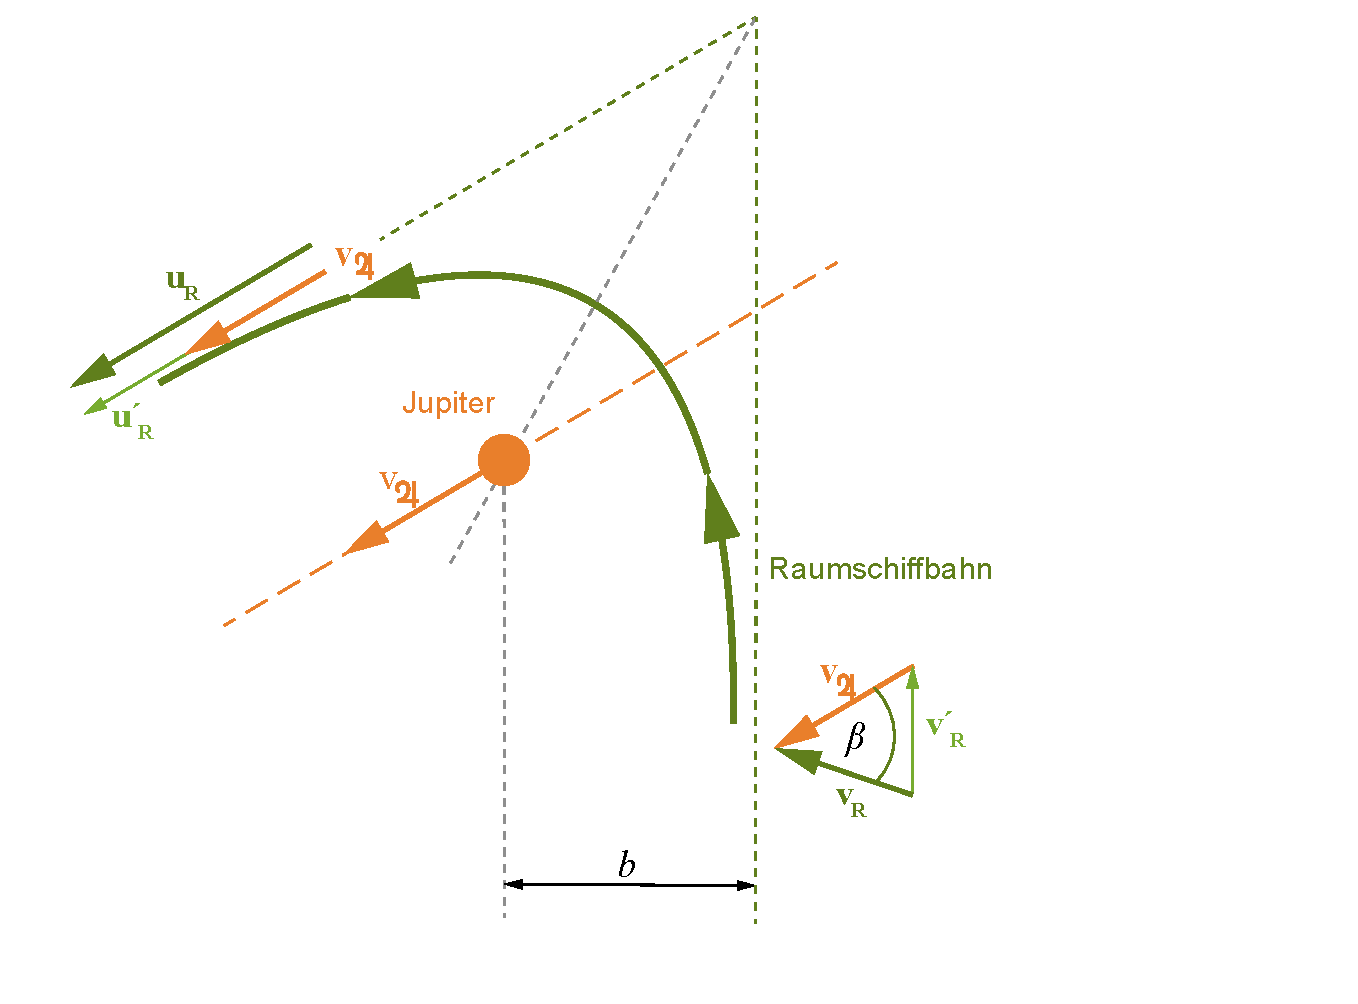
\includegraphics[width=\textwidth]{Lsg_SwingBy.pdf}%
\caption[Geometrie des Swing-By-Man�vers am Jupiter]{Geometrie des Swing-By-Man�vers am Jupiter}
\label{abb:bew_Lsg_SwingBy}
\end{figure}

Zur Berechnung der erreichbaren Geschwindigkeits�nderung braucht man:\\
\begin{tabular}{L{1.5cm}L{10.0cm}}
	$\vec{v}_R$,$\vec{u}_R$ & die Anfangs- bzw. Endgeschwindigkeit des Raumschiffs in $\vec{\Sigma}_\text{L}$, wenn es in den Gravitationsbereich des Jupiters kommt bzw. diesen verl�sst,  \\ 
	$\vec{v}'_R$,$\vec{u}'_R$ & die Anfangs- bzw. Endgeschwindigkeit des Raumschiffs in $\vec{\Sigma}'$, wenn es in den Gravitationsbereich des Jupiters kommt bzw. diesen verl�sst,  \\ 
  $\vec{v}_{\jupiter}$ & die Bahngeschwindigkeit des Jupiters zur Zeit des Vorbeifluges der Raumsonde, die f�r diesen Zeitabschnitt als konstant angesehen wird, \\ 
  $b$ & den Sto�parameter, d.h. den Abstand der einfallenden Asymptote vom Planetenzentrum. \\ 
\end{tabular}\\
Die Geschwindigkeiten der Raumsonde im System $\vec{\Sigma}'$, das hier das Schwerpunktsystem des Jupiters ist, sind gestrichen gekennzeichnet, die ungestrichenen Gr��en beziehen sich auf das Laborsystem $\vec{\Sigma}_\text{L}$, welches das KOS der ruhenden Sonne ist. \\
Es gilt dann:
		\begin{align*}
				\vec{v}_\text{R}&=\vec{v}_\text{R}'+\vec{v}_{\jupiter} \,,~~~~~\vec{u}_\text{R}=\vec{u}_\text{R}'+\vec{v}_{\jupiter} \,. 
		\end{align*}
\newpage
F�r die asymptotischen Hyperbelgeschwindigkeiten (\figref{bew_Lsg_SwingBy}) gilt:
		\begin{align}
				|\vec{v}_\text{R}'|=|\vec{u}_\text{R}'|=\sqrt{{v_\text{R}}^2+{V_{\jupiter}}^2-2v_\text{R}v_{\jupiter}\cos\beta} \,, \label{eq:bew_lsg_SwingBy05}
		\end{align}
worin $\beta$ der Winkel zwischen $\vec{v}_\text{R}$ und $\vec{v}_{\jupiter}$ ist. \\
In den Kapiteln Himmelsmechanik
und Astrodynamik (Band II, Kapitel 3 und 4) wird genauer gezeigt, wie man die Geschwindigkeiten von Planeten und Raumsonden 
bei einer Missionsplanung berechnet.
Hier machen wir nur eine Absch�tzung aus der Umlaufszeit und dem mittleren Bahnradius.
		\begin{align}
				v_{\jupiter} = \frac{2\pi \, a_{\jupiter} }{T_{\jupiter}}  = \frac{2\pi\cdot 5.2\cdot149\cdot10^6 \, \mathrm{km}}{11.9\cdot 365\cdot 86400 \,\mathrm{s}} \approx \SI{12.9}{km\per\second} \,.
		\end{align}
Die maximale Geschwindigkeit des Raumschiffes k�nnen wir wie folgt absch�tzen.
Auf der Erdbahn muss das Raumschiff, die Fluchtgeschwindigkeit
\begin{align*}
	v_\text{F} = \sqrt{\frac{2 G m_{\astrosun}}{a_{\earth}}} \approx 42.1 \,\mathrm{km\,s^{-1}}
\end{align*}
mitbekommen, um unser Sonnensystem verlassen zu k�nnen. %In der Realit�t wird man diesen Wert mit der heutigen Raketentechnik nicht erreichen. \\
Aus dem Energieerhaltungssatz folgt dann in Bahnn�he des Jupiters ($a_{\jupiter} \approx 5.2 a_{\earth}$) die Geschwindigkeit der Raumsonde:
		\begin{align}
				v_\text{R}\approx v_\text{F}\sqrt{\frac{1}{5.2}}\approx 18.5 \,\mathrm{km\,s^{-1}} \,. \label{eq:bew_lsg_SwingBy05a}
		\end{align}
F�r den Winkel $\beta$ k�nnen wir aus der \figref{bew_Lsg_SwingBy} entnehmen:
		\begin{align}
				\cos\beta=\frac{\vec{v_\text{R}}v_{\jupiter}}{|\vec{v_\text{R}}|\cdot|\vec{v_{\jupiter}}|} = \frac{v_\text{RJ}}{v_\text{R}} \,, \label{eq:bew_lsg_SwingBy05b}
		\end{align}
worin $v_\text{RJ}$ die Projektion von $\vec{v_\text{R}}$ auf die Jupiterbahn ist.
Wegen der Drehimpulserhaltung der Raumsonde bezogen auf die Sonne gilt:
		\begin{align}
				L=\underbrace{m\, a_{\jupiter} \, v_\text{RJ}}_{\substack{\text{Drehimpuls bei \linebreak Jupiter}}}=\underbrace{m \, a_{\earth}\,v_\text{FL} }_{\substack{\text{Drehimpuls bei \linebreak Start Erde}}} ~ \nonumber \\
				\longrightarrow v_\text{RJ} = v_\text{F} \frac{a_{\earth}}{a_{\jupiter}}= \frac{1}{5.2}\,v_\text{F} \approx 8.1 \,\mathrm{km \, s^{-1}} \,. \label{eq:bew_lsg_SwingBy05c}
		\end{align}
Damit erhalten wir aus \eqref{eq:bew_lsg_SwingBy05a} $\beta= \arccos\ \lk \sqrt{1/5.2} \rk \approx 64\degree$ \bzw aus \eqref{eq:bew_lsg_SwingBy05}:
		\begin{align*}
				|u_\text{R}'| \approx 17.3 \,\mathrm{km \, s^{-1}}\,.
		\end{align*}
F�r den Geschwindigkeits�bertrag gemessen im $\vec{\Sigma}_\text{L}$ Koordinatensystem erreicht man den Maximalwert, wenn $\vec{u_\text{R}}$ parallel zu $\vec{v_{\jupiter}}$ liegt:
		\begin{align*}
				u_\text{R} &\approx u_\text{R}'+v_{\jupiter} \approx 17.3\, \mathrm{km \, s^{-1}} + 12.9 \,\mathrm{km \, s^{-1}} \approx 30.2\, \mathrm{km \, s^{-1}} \,. 
		\end{align*}
Die Ausgangsgeschwindigkeit ist damit deutlich gr��er ist als die beim Eingang in den Jupiterbereich ($18.5\, \mathrm{km \, s^{-1}}$).
Die Weiterreise zum Saturn ($a_{\saturn} = 9.5\, a_{\earth}$) oder Pluto ($a_{\pluto} = 39.5 \,a_{\earth}$) verk�rzt sich damit um $\approx$ 0.5 \bzw 3.5 Jahre.\\

\newpage
\subprob{(Zusatz) Alternative Betrachtung des Swing-By-Man�vers}

Man kann das Problem auch einfach als Energietransferbetrachtung eines elastischen Sto�es betrachten. 
Allerdings k�nnen wir nicht einfach die Energie�bertragung nach \eqref{eq:bew_Streuung3} nehmen, da diese f�r eine ruhende Masse $m_2$ hergeleitet worden war.
In unserem Fall ist $m_\text{L}= m_{\jupiter}$ und bewegt sich aber im Labor(Sonnen)system mit ca. $v_{\jupiter} = \SI{12.9}{\km\per\second}$.
Wir m�ssen deshalb \eqref{eq:bew_Streuung3} auf den Fall erweitern, dass sich beide Massen bewegen.
Dann braucht man aber zur Auswertung der Gleichung immer noch den Streuwinkel $\vartheta'$, der sich f�r diesen Fall aus der Bewegung im Zentralkraftfeld ableiten l�sst. Dies wird in der Astrodynamik im Band II, Kapitel 4 im  Detail ausgef�hrt.\\
Man kann nat�rlich auch die Bewegungsgleichung der Sonde im Zentralkraftfeld des sich bewegenden Jupiter mit den entsprechenden Anfangsbedingungen numerisch integrieren, um so die genaue Bahn auch unter Einrechnung von St�rgr��en zu berechnen. Es sei auf die numerische Behandlung der Rutherford-Streuung im Kapitel \ref{kap:bew_scatter_problems} \bzw des Swing-By-Man�vers in der Astrodynamik im Band II, Kapitel 4 verwiesen.

\end{subprobs}
\end{sol} 
%\href{PhysikUncut_Part1.pdf#prb:bew_SwingBy}{\textcolor{blue} {$\rightarrow$ zur \probref{bew_SwingBy}.}}\\
\textcolor{blue} {$\rightarrow$ zur} \probref{bew_SwingBy}.\\
\noindent\rule[1ex]{\textwidth}{0.5pt}  \newpage
\medskip

%-----------------------------------------------------------------------------------------------------------
\hypertarget{lsg:bew_Billardspiel}{}
\begin{sol}{prob:bew_Billardspiel}\label{lsg:bew_Billardspiel} %�bung10
\textbf{Billardspiel} \\
\begin{figure}[H]
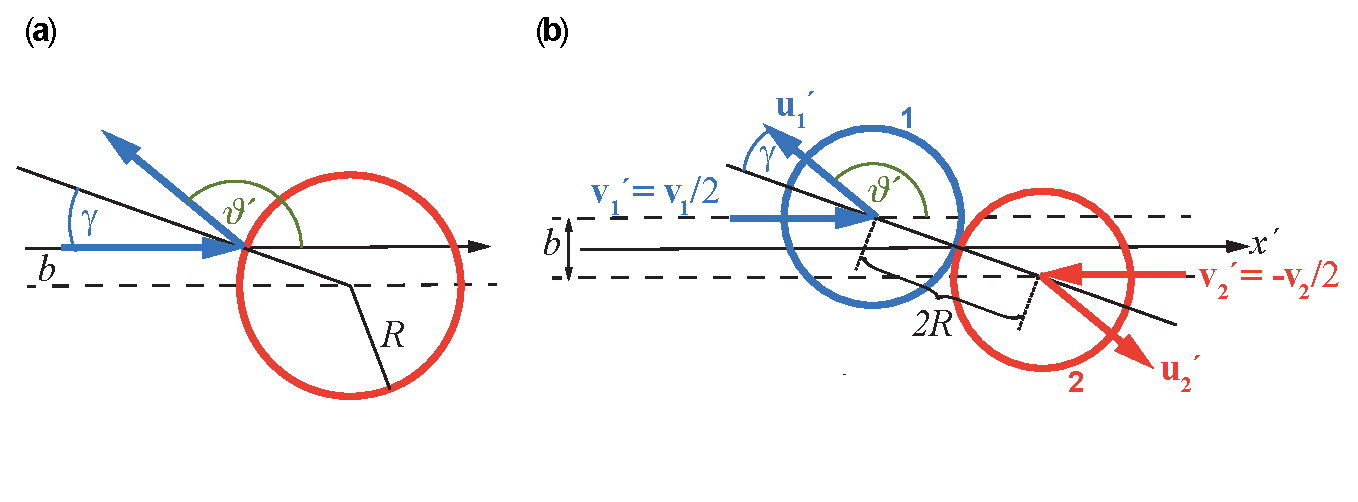
\includegraphics[width=\textwidth]{Billardspiel02.pdf}
\caption[Reflexion eines Teilchens an einer Kugeloberfl�che]{\fa Reflexion eines Teilchens an einer Kugeloberfl�che und \fb Geometrie zweier Billardkugeln im Moment des Zusammensto�es im Schwerpunktsystem $\vec{\Sigma}'$} 
\label{abb:bew_Billardspiel02}
\end{figure}
\begin{subprobs}
\subprob{Wirkungsquerschnitte bei idealer Reflexion.}
Wir betrachten zun�chst die Reflexion eines beliebig kleinen Teilchens an einer Kugeloberfl�che (\figref{bew_Billardspiel02} a). 
Aus der Geometrie erkennt man:
	\[\sin\gamma = \frac{b}{R} \quad  \text{und} \quad \vartheta' = \pi - 2\gamma = \pi - 2 \arcsin\frac{b}{R} \]
	\[\rightarrow b(\vartheta') = R \sin \frac{\pi - \vartheta'}{2} = R \cos \frac{\vartheta'}{2}\,. \]
Mit \eqref{eq:bew_Streuung16} folgt daraus der differentielle Wirkungsquerschnitt:
\begin{align}
	\frac{\D \sigma'}{\D \Omega}  \:=  \frac{1}{2 \sin\vartheta'} \left| \frac{\D b^2(\vartheta')}{\D\vartheta'} \right| = \frac{1}{2 \sin\vartheta'}  \, R^2  \, \cos \frac{\vartheta'}{2}  \, \sin \frac{\vartheta'}{2} = \frac{1}{4} R^2 \,. 
	\label{eq:bew_Billard01}
\end{align}
Der totale Wirkungsquerschnitt ergibt sich durch Integration �ber den Raumwinkel:
		\[\sigma' \:= \int \frac{\D \sigma'}{\D \Omega}  \, \D \Omega = 2 \pi \int\nolimits_{0}^{\pi} \frac{\D \sigma'}{\D \Omega} \sin\vartheta'  \, \D \vartheta' = \frac{\pi R^2}{2} \int\nolimits_{0}^{\pi} \sin\vartheta'  \, \D \vartheta' = \pi R^2 \,.
	\]
Wie nicht anders zu erwarten, ist dies die Querschnittsfl�che der Kugel.

\newpage
\subprob{Wirkungsquerschnitte beim Sto� zweier Kugeln.}
Wir gehen nun zu zwei Kugeln �ber und betrachten \figref{bew_Billardspiel02}\,b.
Wir k�nnen das Ergebnis von Teilaufgabe 1 verwenden, in dem wir $\hat{R} = R_1 + R_2$ setzen und erhalten:
	\[\frac{\D \sigma'}{\D \Omega}  \:=  \frac{1}{4} \hat{R}^2 \,.
	\]
F�r die Umrechnung ins Laborsystem gilt die Gleichung \eqref{eq:bew_Streuung7}, die wir wie folgt umformen:
\begin{align}
	\tan^2\vartheta \lk \cos\vartheta' + \frac{m_1}{m_2} \rk^2 &= 1 -\cos^2\vartheta'  \nonumber \\
	\sin^2\vartheta \lk \cos^2\vartheta' + 2  \, \frac{m_1}{m_2} \, \cos\vartheta' + \lk \frac{m_1}{m_2} \rk^2 \rk &= \cos^2\vartheta -\cos^2\vartheta\cos^2\vartheta' \nonumber \\
	\rightarrow \cos\vartheta' = -\frac{m_1}{m_2} \sin^2\vartheta + \cos\vartheta \sqrt{1 - \lk\frac{m_1}{m_2}\rk^2 \sin^2\vartheta} \,.\label{eq:bew_Billard02}
\end{align}
Daraus berechnet man leicht:
	\[
	\frac{\D \sigma}{\D \Omega} = \frac{\D \sigma'}{\D \Omega} \left| \frac{\D \cos\vartheta'}{\D \cos\vartheta} \right| = \lek 2 \frac{m_1}{m_2} \cos\vartheta + \frac{1 + \lk\frac{m_1}{m_2}\rk^2 \cos(2\vartheta)} {\sqrt{1 - \lk\frac{m_1}{m_2}\rk^2 \sin^2\vartheta}} \rek \frac{\D \sigma'}{\D \Omega} \,,
\]
woraus man mit \eqref{eq:bew_Streuung17} den differentiellen Wirkungsquerschnitt im Laborsystem erh�lt.
F�r $m_1 = m_2$ gilt $\hat{R} = 2R$ und man erh�lt:
	\[\frac{\D \sigma}{\D \Omega} = R^2 \lk 2\cos\vartheta + \frac{1+\cos(2\vartheta)}{\cos\vartheta} \rk = 4 R^2 \cos\vartheta \,.
\]
Die Streuwinkel im Laborsystem als Funktion des Sto�parameters ergeben sich dann zu:
\begin{align}
		\vartheta_1 = \arctan\frac{\sin\vartheta'}{\cos\vartheta'+1} ~~\text{und} ~~ \vartheta_2 = 90\degree - \vartheta'/2 \,. \label{eq:bew_Billard03}
\end{align}
\subprob{Berechnung des Sto�parameters.}
Um den Sto�parameter zu berechnen, bei dem die gesto�ene Kugel unter einem Winkel von $60 \degree$ wegrollt, wird \eqref{eq:bew_Billard02} nach $\vartheta'$ gel�st.
Wir erhalten: $\vartheta' = 2 \vartheta_1 = 120\degree$, woraus $\vartheta_2 = 30\degree$ folgt.
Das Ergebnis h�tte man nat�rlich auch direkt aus dem Impuls- und Energieerhaltungssatz ableiten k�nnen, es ging hier aber darum, die grunds�tzliche Vorgehensweise bei Streuproblemen zu beleuchten.
Welche Energie wird �bertragen?
Hier benutzen wir \eqref{eq:bew_Streuung9} und erhalten einen Energie�bertrag auf Kugel 2 von:
\begin{align}
	\frac{\Delta T}{T_1^{\text{(init)}}} = \frac{1}{2} \lk \cos\vartheta' -1 \rk =  -\frac{3}{4} = -75\,\% ~, \label{eq:bew_Billard04}
\end{align}
was bedeutet, dass $75\,\%$ der kinetischen Energie von Kugel 1 auf Kugel 2 �bertragen werden.
\end{subprobs} 
Die Ergebnisse der Rechnungen sind in \mlbewref{Billardspiel.m} ausgef�hrt und in \figref{bew_Billardspiel03} gezeigt.\\

\begin{figure}[H]
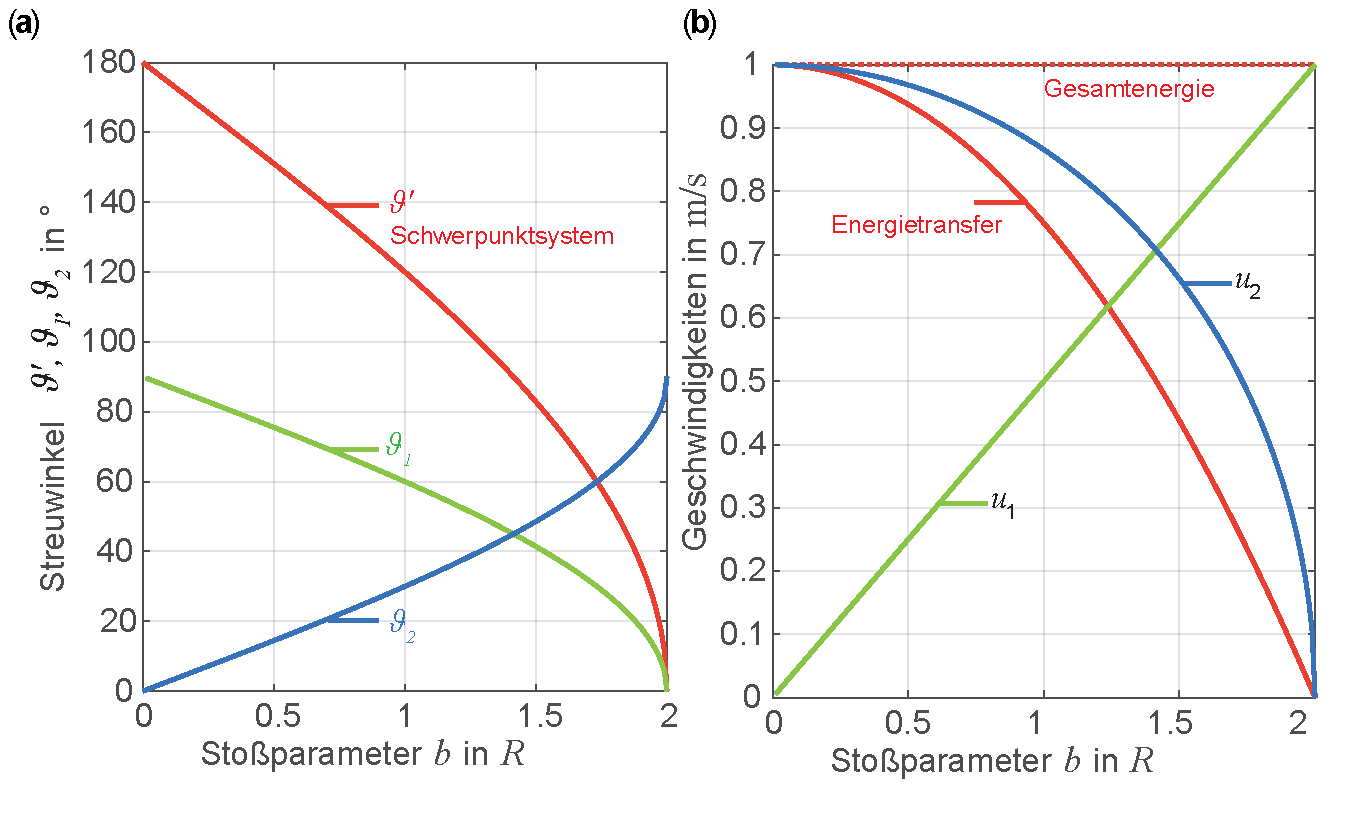
\includegraphics[width=\textwidth]{Billardspiel03.pdf}
\caption[Streuwinkel und Geschwindigkeiten zweier Billardkugeln]{\fa Streuwinkel und \fb Geschwindigkeiten und Energietransfer nach Zusammensto� zweier identischer Billardkugeln, von denen eine ruht und die andere mit $v=\SI{1}{\metre\per\second}$ gesto�en wird}
\label{abb:bew_Billardspiel03}
\end{figure}

\end{sol} 
%\href{PhysikUncut_Part1.pdf#prb:bew_Billardspiel}{\textcolor{blue} {$\rightarrow$ zur \probref{bew_Billardspiel}.}}\\
\textcolor{blue} {$\rightarrow$ zur} \probref{bew_Billardspiel}.\\
\noindent\rule[1ex]{\textwidth}{0.5pt}  \newpage

%-----------------------------------------------------------------------------------------------------------
\hypertarget{lsg:bew_HillLagrangePkt}{}
\begin{sol}{prob:bew_HillLagrangePkt}\label{lsg:bew_HillLagrangePkt} %�bung11
\textbf{Hill-Kurve und Lagrange-Punkte.} \\ \\
	F�r das Sonne-Planeten-System (z.B. Sonne-Erde) ist die Geometrie gegeben durch 
	\[  1 - q = \frac{m_2}{m_2 + m_1} = \frac{1}{1+ {m_1}/{m_2}} < 1
	\]
	%und den Ortsvektoren
	%\[\vec{r_1} = \lk (q-1)a,0,0 \rk  \qquad , \qquad \vec{r_2}=\lk qa,0,0 \rk \] 
	%und $\vec{\omega}=(0,0,\omega)$.
	% Vektorschreibweise:
		und den Ortsvektoren $\vec{r}_1, \vec{r}_2$
	\[
		\vec{r_1} = \lk \begin{array} {c}
	 	(q-1)\,a \\ 0\\ 0
	 \end{array} \rk, \qquad
		\vec{r_2} = \lk \begin{array} {c}
	 	q\,a \\ 0\\ 0 
		\end{array} \rk  \quad \text{sowie der Umlaufkreisfrequenz} \quad
		\vec{\omega} = \lk \begin{array} {c}
	 	0 \\ 0\\ \omega 
	 \end{array} \rk \,.
	\]
	Hierbei haben wir die Bahnebene als $x$-$y$-KOS verwendet und den Nullpunkt in den Schwerpunkt des Systems gelegt.
	Wir k�nnen damit das effektive Potential $\hat{U}_\text{eff}$ berechnen, welches auf eine Testmasse (z.B. Satelliten) $m_3$ und auf die Gravitationskonstante $G$ normiert ist:
	\[\hat{U}_\text{eff}(x_3,y_3) = \frac{U_\text{eff}}{G m_3} = -\frac{m_1}{d_1(x_3,y_3)} - \frac{m_2}{d_2(x_3,y_3)} - \frac{m_1 + m_2}{2a^3}({x_3}^2 + {y_3}^2) ~,
	\]
	wobei
	\begin{align*}
		d_1 &= \sqrt{\lk x_3 - (q-1)\,a\rk^2 + {y_3}^2} = d_1(x_3,y_3) \qquad \text{und} \\
		d_2 &= \sqrt{\lk x_3 - q\,a\rk^2 + {y_3}^2} = d_2(x_3,y_3)~.
	\end{align*}
	Die entsprechende allgemeine Rechnung ist in \mlbewref{LagrangePunkte.m} ausgef�hrt.
	In \figref{bew_3KoerperP03} sind die Lagrange-Punkte und Hill-Kurven f�r ein dem Sonne-Jupiter-�hnlichen System mit $m_1/m_2 = 1000$ und einem hypothetischen System mit einem Massenverh�ltnis von $m_1/m_2 = 10$ dargestellt. 
	Auch f�r  das Erde-Mond-System (mit einem Massenverh�ltnis von $m_1/m_2 \approx 333 000$) bleibt die grunds�tzliche geometrische Lage der Lagrange-Punkte erhalten. 
	Sie sind jeweils lokale Maxima des effektiven Potentials, die aber mathematisch instabile Gleichgewichtspunkte sind, wie man durch nochmalige Ableitung von ${\partial}/{\partial \vec{r}_3} \,\lk U_\text{eff} \rk$ zeigen kann.\\
Dass sich \zb ein Raumschiff dennoch relativ stabil
an einem Lagrange-Punkt aufhalten kann, wird in der Astrodynamik im Band II, Kapitel 4 durch eine entsprechende
Stabilit�tsanalyse gezeigt.
Ursache daf�r ist das Wirken der Coriolis-Kraft in den Bewegungsgleichungen \eqref{eq:bew_red3KP07}.\\

\begin{figure}[H]
\includegraphics[width=\textwidth]{LagrangePt.pdf}
\caption[Lagrange-Punkte und Hill-Kurven Sonne-Planeten-Satelliten-Systeme]{Lagrange-Punkte und Hill-Kurven f�r zwei Sonne-Planeten-Satelliten-Systeme} 
\label{abb:bew_3KoerperP03}
\end{figure}

\end{sol} 
%\href{PhysikUncut_Part1.pdf#prb:bew_HillLagrangePkt}{\textcolor{blue} {$\rightarrow$ zur \probref{bew_HillLagrangePkt}.}}\\
\textcolor{blue} {$\rightarrow$ zur} \probref{bew_HillLagrangePkt}.\\
\noindent\rule[1ex]{\textwidth}{0.5pt}  \newpage

%-----------------------------------------------------------------------------------------------------------
\hypertarget{lsg:bew_gezeiten01}{}
\begin{sol}{prob:bew_gezeiten01}\label{lsg:bew_gezeiten01} %�bung12
\textbf{Gezeitenkr�fte.} \\

Wir wollen die Verformung eines Masserings unter dem Einfluss von Gezeitenkr�ften berechnen. Den Ring beschreiben wir als Anordnung von 36 Testmassen, die im Schwerefeld einer gro�en Masse frei fallen. Wir betrachten dazu die Geometrie nach \figref{bew_lsggezeiten01}. \\
Wir k�nnen die Massen $m_1$ bis $m_{17}$ und $m_{19}$ bis $m_{35}$ wie folgt behandeln:
\begin{align*}
    \varphi_i\lk 0\rk = i\cdot 10\degree && i = 1\ldots 17, 19\ldots 35
\end{align*}
Nach dem Sinussatz gilt zum Zeitpunkt $t=0$:
\begin{align}
    \frac{\sin\alpha_i}{R} &= \frac{\sin\varphi_i\lk 0\rk}{r_i\lk 0 \rk}  \label{eq:bew_lsggezeiten01} \\
    \rightarrow ~~~~ \sin\alpha_i &= \frac{R}{r_0}\,\frac{\sin\varphi_i\lk 0\rk}{\sqrt{q-2\,\frac{R}{r_0}\,\cos\varphi_i\lk 0\rk + \frac{R^2}{r_0{}^2}}}\;. \nonumber
\end{align}
Der Winkel $\alpha_i$ ist f�r jede Masse konstant �ber die Zeit, wenn wir wie angenommen alle $m_i \ll M$ annehmen.\\
Die Newtonschen Bewegungsgleichungen lauten dann im gew�hlten KOS nach \figref{bew_lsggezeiten01}:
\begin{align}
\begin{split}
    \ddot{x}_i &= -\frac{M\,G}{x_i{}^2+z_i{}^2}\,\sin\alpha_i\,, \\
    \ddot{z}_i &= -\frac{M\,G}{x_i{}^2+z_i{}^2}\,\cos\alpha_i\,.
\end{split} \label{eq:bew_lsggezeiten02}
\end{align}
Die Anfangsbedingungen sind gegeben durch:
\begin{align*}
    x_i\lk 0\rk &= R\,\sin\varphi_i \,,\\
    z_i\lk 0\rk &= r_0 - R\,\cos\varphi_i \,.
\end{align*}
F�r die Massen $m_0$, $m_{18}$ und $m_z$ vereinfacht sich das System, da $\alpha_0 = \alpha_{18} = \alpha_z = 0$ zu
\begin{align}
    \ddot{z}_i = -\frac{M\,G}{z_i{}^2}\,. \label{eq:bew_lsggezeiten03}
\end{align}
Wir l�sen die DGL-Systeme \eqref{eq:bew_lsggezeiten02} und \eqref{eq:bew_lsggezeiten03} numerisch (\mlbewref{Gezeitenkraefte.m}).
Die L�sung ist in \figref{bew_lsggezeiten01} dargestellt.
Wir erkennen wie sich der Ring verformt.
In unserem Fall, in dem wir $M\gg m$ angenommen haben und auch $r_0$ nur wenig gr��er als $R$ ist die Gezeitenkraft f�r die Masse $m_{18}$ deutlich kleiner als f�r die Masse $m_0$, $m_{17} < m_1$ \usW
Folglich verformt sich der Ring nicht zu einem Ellipsoid, sondern zu einer birnenf�rmigen Anordnung von Massen. \\

\begin{figure}[H]
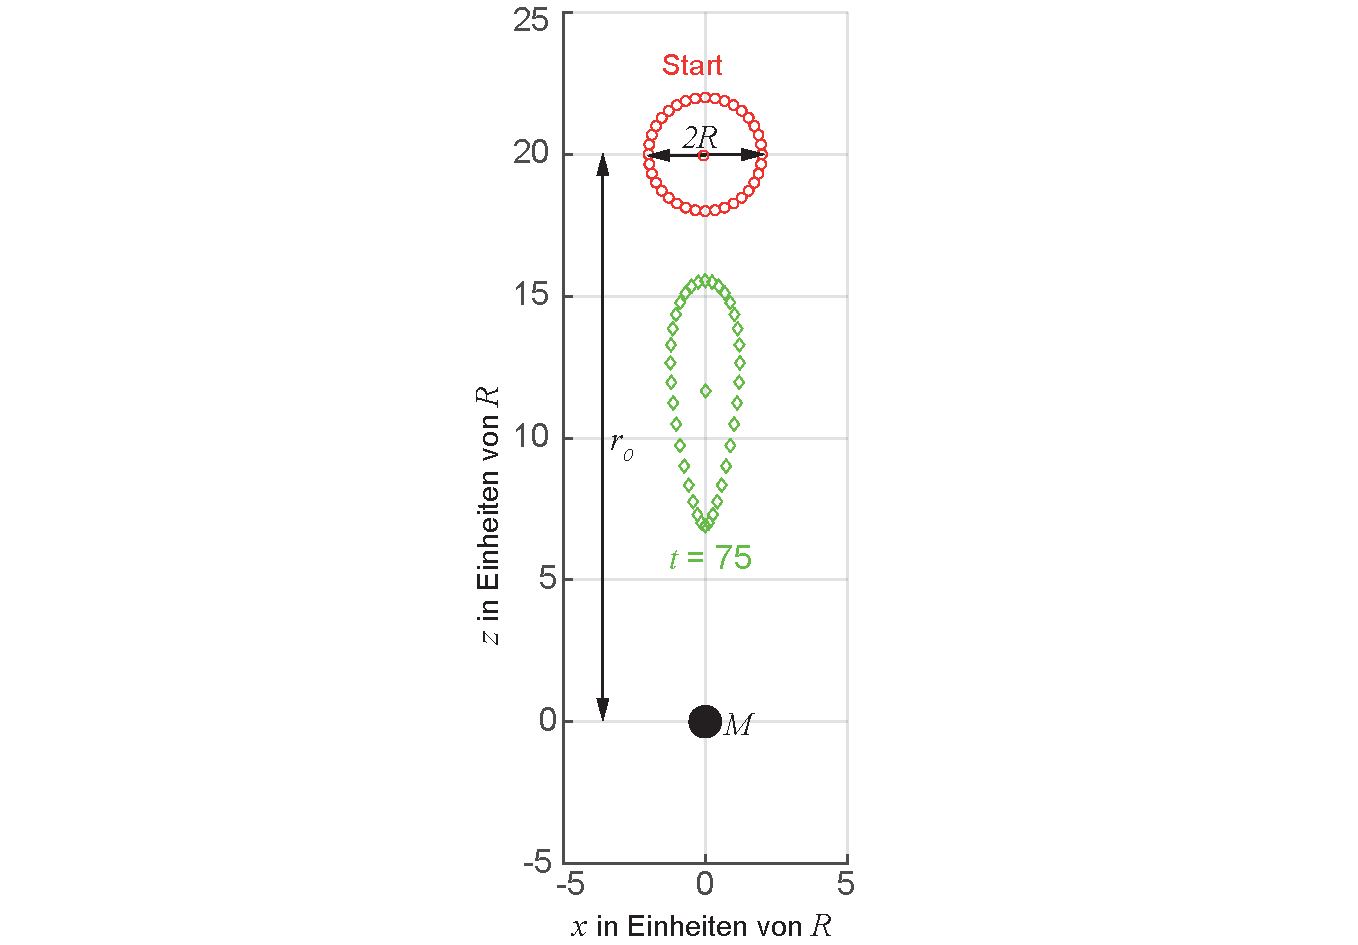
\includegraphics[width=\textwidth]{Gezeitenkraefte.pdf}
\caption[Gezeitenwirkung auf einen Ring]{Gezeitenwirkung auf einen Ring aus 36 Massepunkten. Parameter: $r_0 = 20 R, R = 2, M\,G = 1$}
\label{abb:bew_lsggezeiten01}
\end{figure}

F�r den mathematisch interessierten Leser geben wir noch eine analytische L�sung f�r \eqref{eq:bew_lsggezeiten03}, wobei diese nicht wirklich einen gro�en Vorteil bietet, da sie nur eine analytische L�sung f�r $t\lk z\rk$ liefert, man also auch noch numerisch die Umkehrfunktion $z\lk t\rk$  bestimmen muss. Wir schreiben dazu f�r \eqref{eq:bew_lsggezeiten03}:
\begin{align*}
    \ddot{z} &= \frac{A}{z^2} ~~~~ \text{mit} ~~~~ A=-M\,G \\
    A-\ddot{z}\,z^2 &= 0 ~~~~| \dot{z} ~~\rightarrow ~~ \frac{A\,\dot{z}}{z^2} = \dot{z}\,\ddot{z}
\end{align*}
Mit $\frac{\D}{\D t}\,\lk \dot{z}\rk^2 = 2\dot{z}\,\ddot{z}$ und $\frac{\D}{\D t}\,\lk -\frac{A}{z}\rk = \frac{A\,\dot{z}}{z^2}$ erhalten wir:
\begin{align*}
    C_1 -\frac{A}{z} = \frac{1}{2}\,\dot{z}^2\,,
\end{align*}
worin $C_1$ eine Integrationskonstante ist, die sich aus dem AB ergibt.
\begin{align*}
    \sqrt{2C_1 - \frac{2A}{z}} &= \dot{z}\,~~\rightarrow~~ \D t = \frac{\D z}{\sqrt{2C_1-\frac{2A}{z}}} = \frac{\D z}{\sqrt{2}\sqrt{C_1-\frac{A}{z}}}\,.
\end{align*}

\newpage
Aus Integraltafeln (\zb \cite{Gradshteyn1980}) finden wir 
\begin{align}
\begin{split}
    \int\limits_0^t \D t &= t = \int\limits_{z_0}^t \frac{\D z}{\sqrt{C_1 - \frac{A}{z}}} ~~~~~~~~ 2C_1 \rightarrow C_1 \\
    &= \frac{z\,\sqrt{C_1 - \frac{2A}{z}}}{C_1} + \frac{2A\,\arctan\lek \frac{\sqrt{C_1-\frac{2A}{z}}}{\sqrt{C_1}}\rek}{\sqrt{C_1{}^3}}
\end{split} \label{eq:bew_lsggezeiten04}
\end{align}
Wenn man $z\lk t \rk$ haben will, muss man wie gesagt \eqref{eq:bew_lsggezeiten04} ebenfalls numerisch l�sen. 

\end{sol} 
%\href{PhysikUncut_Part1.pdf#prb:bew_gezeiten01}{\textcolor{blue} {$\rightarrow$ zur \probref{bew_gezeiten01}.}}\\
\textcolor{blue} {$\rightarrow$ zur} \probref{bew_gezeiten01}.\\
\noindent\rule[1ex]{\textwidth}{0.5pt}  \newpage

%----------------------------------------------------------------------------------
\hypertarget{lsg:bew_Zwangsbedingungen}{}
\begin{sol}{prob:bew_Zwangsbedingungen}\label{lsg:bew_Zwangsbedingungen}%�bung13
\textbf{Zwangsbedingungen} 
\begin{subprobs}

\subprob{Perle auf 2D-Spirale}
	Wir betrachten zun�chst eine Spirale im $R^2$, d.h. in einer Ebene, auf der sich eine Perle bewegt.
        Die Spirale sei eine logarithmische Spirale:
	\begin{align*}
	r(\varphi) = a\mathrm{e}^{k\varphi}~.
	\end{align*} 
	Hierbei sind $a$ und $k$ feste Parameter.
	Daraus folgt die Zwangsbedingung: 
	\begin{align}
	a\mathrm{e}^{k\varphi}-r=0 \label{eq:lsg_bew_bed1}
	\end{align}
	$\rightarrow$ Kategorie: holonom-skleronom, ein Freiheitsgrad ($\varphi$).

\subprob{Perle auf eing�ngiger Helix}
	Wir betrachten nun eine Spirale im $R^3$, auch Helix genannt.
        Eine solche kann man sich vorstellen wie die in Kugelschreibern verbauten Stahlfedern.
        Die Bewegung einer Perle auf dieser Spirale kann in kartesischen Koordinaten wie folgt beschrieben werden: 
	\begin{align}
	\vec{x} =
	\begin{pmatrix}
	\varrho_0 \cos \varphi \\
	\varrho_0 \sin \varphi \\
	h \varphi
	\end{pmatrix}.
	\label{eq:lsg_bew_log_helix1}
	\end{align}
	Die beiden Zwangsbedingungen f�r Zylinderkoordinaten lauten:
	\begin{align}
	\varrho - \varrho_0 &= 0  &  z - h \varphi &= 0 \,. \label{eq:lsg_bew_log_helix2}
	\end{align}
	Dabei ist $h$ die Gangh�he der Helix und $\varphi$ als Winkel (in Bogenma�) die freie Variable.\\
	$\rightarrow$ Kategorie: holonom-skleronom, ein Freiheitsgrad ($\varphi$).

\subprob{Sph�risches Pendel}
	Der Massepunkt eines sph�rischen Pendels bewegt sich auf einer Kugeloberfl�che.
        Der Abstand zum Mittelpunkt dieser Kugel betr�gt damit f�r jeden m�glichen Aufenthaltsort des Massepunktes $R$.
        Dies ergibt die einfache Zwangsbedingung:
	\begin{align}
	x^2+y^2+z^2-R^2=0 \,, \label{eq:lsg_bew_SPen}
	\end{align}
	bzw. in sph�rischen Koordinaten: $r - R =0$.
        Es verbleiben zwei Freiheitsgrade.
	Als freie bzw. verallgemeinerte Koordinaten werden die beiden Winkel $\varphi$ und $\vartheta$ gew�hlt.
	\\
	$\rightarrow$ Kategorie: holonom-skleronom, zwei Freiheitsgrade ($\varphi$) und ($\vartheta$).

\begin{figure}[H]
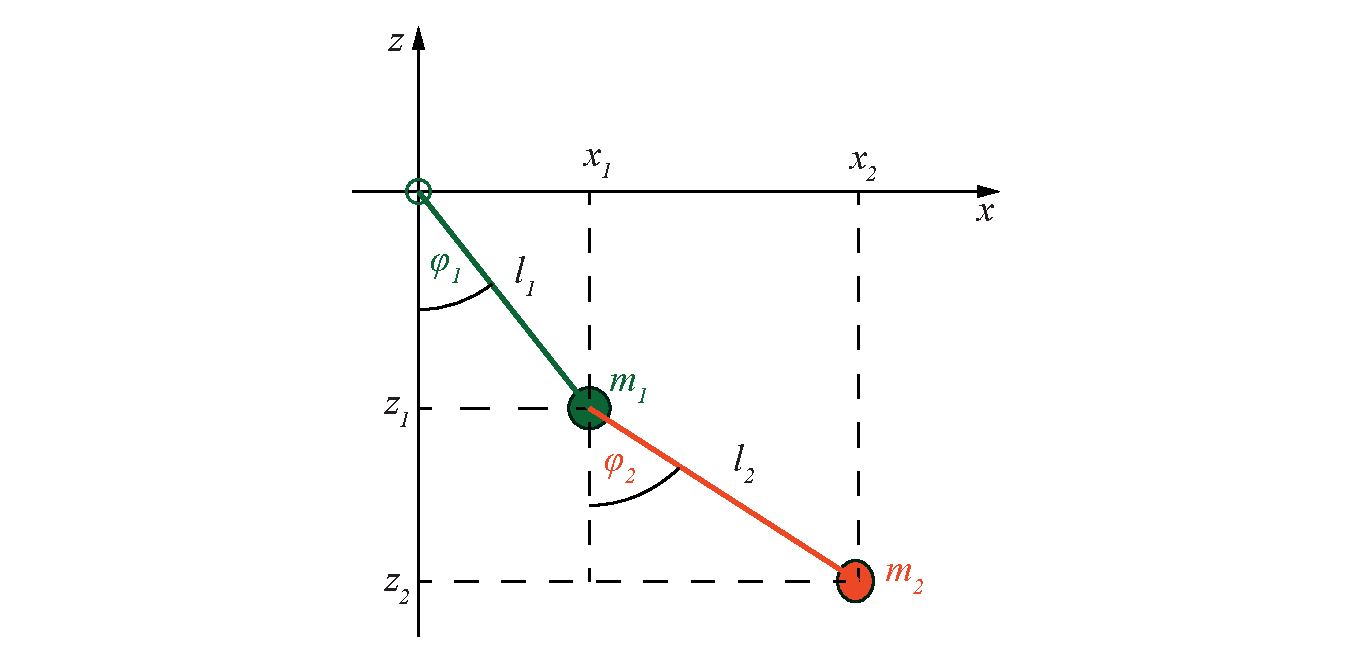
\includegraphics[width=\textwidth]{UebungDoppelpendel.pdf}%
\caption[Doppelpendel]{Doppelpendel}
\label{abb:bew_lsg_Doppelpendel}
\end{figure}

\subprob{Doppelpendel}
	Die Bewegung soll in der $x$-$z$-Ebene erfolgen.
        Um die Zwangsbedingungen eines (ebenen) Doppelpendels aufzustellen, betrachten wir zun�chst das einfaches Pendel mit dem Massepunkt $m_1$ und den kartesischen Koordinaten $x_1,y_1,z_1$.
        Dieser befindet sich im Abstand $l_1$ zum Aufh�ngepunkt.
        Daraus folgt die Zwangsbedingung:
	\begin{align}
		x_1^2+z_1^2-l_1^2=0 \,. \label{eq:lsg_bew_DPen1}
	\end{align}
	Wir betrachten nun einen zweiten Massepunkt $m_2$ mit den Koordinaten $x_2,y_2,z_2$, der �ber die feste  L�nge $l_2$ mit $m_1$ verbunden ist.
        Daraus folgt mit dem Abstand der beiden Punkte die zweite Zwangsbedingung:
	\begin{align}
	\Delta x^2 + \Delta z^2 &= l_2^2 \nonumber \\
	(x_2-x_1)^2 + (y_2-y_1)^2 - l_2^2 &= 0 \,. \label{eq:lsg_bew_DPen4}
	\end{align}
	Es gibt f�r die Bewegung in der $x$-$z$-Ebene also zwei Zwangsbedingungen und somit $4 - 2 = 2$ Freiheitsgrade.
        F�r diese bieten sich als generalisierte Koordinaten die Winkel $\varphi_1$ und $\varphi_2$ an.
        Die Transformation lautet:
	\begin{align*}
	\vec{r}_1 &= \begin{pmatrix} 
	l_1 \sin\varphi_1 \\ 
	0 \\ 
	-l_1 \cos\varphi_1  
	\end{pmatrix} & 
	\vec{r}_2 &= \begin{pmatrix} 
	l_1 \sin\varphi_1 + l_2 \sin\varphi_2 \\
	 0 \\
	  -l_1 \cos\varphi_1 - l_2 \cos\varphi_2 
	  \end{pmatrix}.
	\end{align*}
	$\rightarrow$ Kategorie: holonom-skleronom, zwei Freiheitsgrade ($\varphi_1$) und ($\varphi_2$).

\newpage
\subprob{Pendel mit vertikal schwingender Aufh�ngung}
	Das in der $x$-$z$-Ebene schwingende Pendel mit der L�nge $l$ ist am Aufh�ngepunkt mit Koordinaten $x_\text{A}=0, z_\text{A}$ befestigt, welcher mit einer Frequenz $\Omega$ schwingt.
        Es ist also $z_\text{A}=A\sin(\Omega t - \varphi_\text{A})$.
        Der am unteren Ende h�ngende Massepunkt hat die Koordinaten $x, y$. 
	Als Zwangsbedingung gilt generell f�r das Pendel
	\begin{align}
	\lk x-x_\text{A} \rk^2+ \lk z-z_\text{A} \rk^2-l^2=0 \, \label{eq:lsg_bew_PvA1} 
	\end{align}
	mit den Transformationen
	\begin{align}
	x &= l\sin \varphi \nonumber \\
	z &= A\sin(\Omega t - \varphi_\text{A}) - l \cos\varphi \,. \label{eq:lsg_bew_PvA2}
	\end{align} 
	$\rightarrow$ Kategorie: holonom-rheonom, ein Freiheitsgrad ($\varphi$).

\subprob{Pendel mit horizontal schwingender Aufh�ngung}
	Analog zur vorherigen Aufgabe k�nnen wir nun f�r die Transformationen formulieren: 
	\begin{align}
	x &= A\sin(\Omega t - \varphi_\text{A}) + l \sin\varphi \nonumber \\
	z &= -l \cos\varphi\,. \label{eq:lsg_bew_PvA3}
	\end{align}
	$\rightarrow$ Kategorie: holonom-rheonom, ein Freiheitsgrad ($\varphi $).

\subprob{Stehendes Pendel mit vertikal schwingendem Boden}
	Dies ist die Umkehrung des h�ngenden Pendels mit vertikal schwingender Aufh�ngung. 
	\begin{align}
	x &= l\sin \varphi \nonumber \\
	z &= A\sin(\Omega t - \varphi_\text{A}) + l \cos\varphi \,. \label{eq:lsg_bew_PvA4}
	\end{align} 
	$\rightarrow$ Kategorie: holonom-rheonom, ein Freiheitsgrad ($\varphi $).

\subprob{Jo-Jo}
	Die Bewegung findet wieder in der $x$-$z$-Ebene statt.
        Die Koordinaten beschreiben den Mittelpunkt des Jo-Jos.
        Aus der \figref{bew_lsg_JoJo} ergeben sich direkt die Zwangsbedingungen:
	\begin{align}
	  x &= 0 \\
	  z + r \varphi &= 0 \, 	\label{eq:lsg_bew_PvA5}
	\end{align}
	wobei das $\varphi > 0$ f�r das aufsteigende und $\varphi < 0$ f�r das absteigende Jo-Jo ist.\\
	$\rightarrow$ Kategorie: holonom-skleronom, ein Freiheitsgrad ($\varphi$).

\begin{figure}[H]
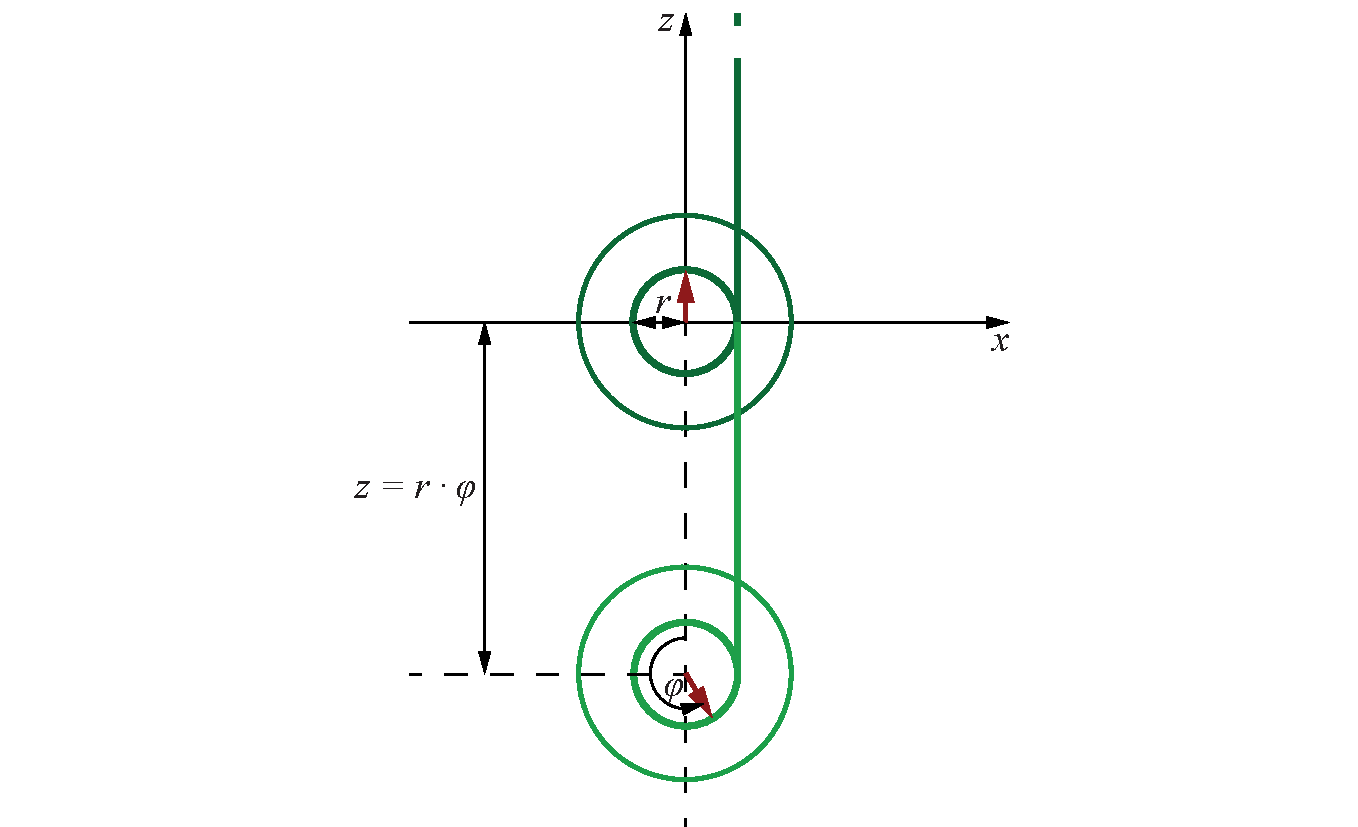
\includegraphics[width=\textwidth]{UebungJoJo.pdf}%
\caption[Akademisches Jo-Jo]{Akademisches Jo-Jo}
\label{abb:bew_lsg_JoJo}
\end{figure}

\end{subprobs} 
\end{sol} 
%\href{PhysikUncut_Part1.pdf#prb:bew_Zwangsbedingungen}{\textcolor{blue} {$\rightarrow$ zur \probref{bew_Zwangsbedingungen}.}}\\
\textcolor{blue} {$\rightarrow$ zur} \probref{bew_Zwangsbedingungen}.\\
\noindent\rule[1ex]{\textwidth}{0.5pt}  \newpage

%-----------------------------------------------------------------------------------------------------------
\hypertarget{lsg:bew_LagrangeII_a}{}
\begin{sol}{prob:bew_LagrangeII_a}\label{lsg:bew_LagrangeII_a}%�bung14
\textbf{Lagrange-Gleichung zweiter Art in Kugelkoordinaten} 
\begin{subprobs}
\subprob{Freies Teilchen}
Die Koordinaten des Massepunktes liegen in sph�rischen Koordinaten $(r, \vartheta, \varphi)$ vor.
Diese k�nnen wie folgt in kartesische Koordinaten umgerechnet werden:  
\begin{align}
x &= r\sin\vartheta\cos\varphi	\nonumber  \\ 
y &= r\sin\vartheta\sin\varphi	\nonumber  \\ 
z &= r\cos\vartheta \,. \label{eq:lsg_bew_LagrangeII_a_01}
\end{align}
Es gibt bei einem freien Teilchen keine Zwangsbedingungen, d.h. es m�ssen alle drei Koordinaten ber�cksichtigt werden.
Um die kinetische Energie $T$ in Kugelkoordinaten zu erhalten, m�ssen alle Koordinaten nach der Zeit abgeleitet werden, da alle drei Koordinaten von der Zeit abh�ngen.
Das Ergebnis lautet:
\begin{align}
\dot{x} &= \dot{r}\sin\vartheta\cos\varphi + r \, \dot{\vartheta}\cos\vartheta\cos\varphi - r \, \dot{\varphi}\sin\vartheta\sin\varphi \nonumber  \\ 
\dot{y} &= \dot{r}\sin\vartheta\sin\varphi + r \, \dot{\vartheta}\cos\vartheta\sin\varphi + r \, \dot{\varphi}\sin\vartheta\cos\varphi \nonumber  \\ 
\dot{z} &= \dot{r}\cos\vartheta - r \, \dot{\vartheta}\sin\vartheta \,. \label{eq:lsg_bew_LagrangeII_a_02}
\end{align}
Die kinetische Energie berechnet sich damit zu: 
\begin{align}
T &= \frac{m}{2} \lk\dot{x}^2 + \dot{y}^2 + \dot{z}^2\rk = \frac{m}{2} \lk\dot{r}^2 + r^2(\dot{\vartheta}^2 + \dot{\varphi}^2\sin^2\vartheta)\rk. \label{eq:lsg_bew_LagrangeII_a_03}
\end{align}
Der Umformungsschritt besteht vor allem in der mehrfachen Anwendung der trigonometrischen Identit�t $\sin^2x + \cos^2x = 1$.
Man erkennt, dass in \eqref{eq:lsg_bew_LagrangeII_a_03} keine gemischten Terme der Ableitungen der Ableitungen $\dot{r}, \dot{\vartheta}, \dot{\varphi}$ vorkommen. 
Mit dem Potential $U=U(r,\vartheta, \varphi)$ und der allgemeinen Lagrange-Funktion $\mathcal{L} = T - U$ erhalten wir die Lagrange-Gleichungen f�r die drei generalisierten Koordinaten $q = \{r, \vartheta, \varphi\}$ nach
\begin{equation}
	\frac{d}{dt} \frac{\d\mathcal{L}}{\d\dot{q}} - \frac{\d\mathcal{L}}{\d q} = 0~.
\end{equation}
Es ergeben sich dann folgende Lagrange-Gleichungen
\begin{align}
	\text{...f�r } r&:  & \frac{d}{dt}(m \, \dot{r})-m \, r \, (\dot{\vartheta}^2+\dot{\varphi}^2\sin^2\vartheta) &= \frac{\d U}{\d r}  \nonumber  \\ 
	\text{...f�r } \vartheta&:  & \frac{d}{dt}(m \, r^2 \, \dot{\vartheta}) - m r^2\dot{\varphi}^2\sin\vartheta \, \cos\vartheta &= \frac{\d U}{\d \vartheta}  \nonumber  \\ 
	\text{...f�r }\varphi&:  & \frac{d}{dt}(m \, r^2\sin^2\vartheta \, \dot{\varphi}) &= \frac{\d U}{\d \varphi} \,. \label{eq:lsg_bew_LagrangeII_a_04}
\end{align}
Diese Berechnung ist wesentlich einfacher als die in \probref{bew_KOS_Formel} durchgef�hrte Berechnung der Beschleunigung �ber die Ableitung der Geschwindigkeit. 

\newpage
\subprob{Teilchen auf Trichter}
Bewegt sich das Teilchen auf der Oberfl�che des kegelf�rmigen Trichters ist die Zwangsbedingung holonom und lautet mit $\vartheta_0$ als dem �ffnungswinkel des Kegels: 
\begin{align}
f = \vartheta - \vartheta_0 = 0 \,. \label{eq:lsg_bew_LagrangeII_a_05}
\end{align}
Dadurch gibt es nur noch zwei unabh�ngige Parameter, den Radius $r$ und den Winkel $\varphi$.
Die Lagrange-Funktion vereinfacht sich dann zu: 
\begin{align}
\mathcal{L} = \frac{m}{2}(\dot{r}^2 + r^2\dot{\varphi}^2 \, \sin^2\vartheta_0)-U(r) \,. \label{eq:lsg_bew_LagrangeII_a_06}
\end{align}
Die Lagrange-Gleichungen in $r$ und $\varphi$ lauten dann: 
\begin{align}
\frac{d}{dt}(m \, \dot{r}) - m \, r \, \dot{\varphi}^2 \, \sin^2\!\vartheta_0 + \frac{\d U}{\d r} &= 0 \nonumber  \\ 
\frac{d}{dt}(m \, r^2 \, \sin^2\!\vartheta_0 \, \dot{\varphi}) = \frac{d}{dt}p_\varphi &= 0 \,. \label{eq:lsg_bew_LagrangeII_a_07}
\end{align}
Der konjugierte Impuls $p_\varphi$ (entspricht hier dem Drehimpuls) ist erhalten und kann verwendet werden, um $\dot{\varphi}$ aus der Bewegungsgleichung f�r $r$ zu eliminieren: 
\begin{align}
\dot{\varphi} = \frac{p_\varphi}{m \, r^2 \, \sin^2\!\vartheta_0} \,. \label{eq:lsg_bew_LagrangeII_a_08}
\end{align}
Wir verwenden wieder das effektive Potenzial $U_\text{eff}$ aus \eqref{eq:bew_Eff_Potential} und schreiben obige Gleichung als: 
\begin{align}
m \, \ddot{r} &= -\frac{\d U}{\d r} + \frac{{p_\varphi}^2 m \, r \, \sin^2\!\vartheta_0}{m^2 \, r^4 \, \sin^4\!\vartheta_0} \nonumber  \\
&= -\frac{\d}{\d r} U + \frac{{p_\varphi}^2}{m \, r^3 \, \sin^2\!\vartheta_0} \nonumber  \\
&= -\frac{\d}{\d r} \lk U + \frac{{p_\varphi}^2}{2m \, r^2 \, \sin^2\!\vartheta_0} \rk = -\frac{\d}{\d r} U_\text{eff} \,. \label{eq:lsg_bew_LagrangeII_a_09}
\end{align}
Interessanterweise f�hrt diese Gleichung f�r $\vartheta_0=90\degree$ genau auf die beschreibenden Formeln des Zweik�rperproblems, welches wir in Kap \ref{kap:bew_ZKP_NZKF} behandelt haben.
\end{subprobs}
\end{sol} 
%\href{PhysikUncut_Part1.pdf#prb:bew_LagrangeII_a}{\textcolor{blue} {$\rightarrow$ zur \probref{bew_LagrangeII_a}.}}\\
\textcolor{blue} {$\rightarrow$ zur} \probref{bew_LagrangeII_a}.\\
\noindent\rule[1ex]{\textwidth}{0.5pt}  \newpage

%-----------------------------------------------------------------------------------------------------------
\hypertarget{lsg:bew_LagrangeII_b}{}
\begin{sol}{prob:bew_LagrangeII_b}\label{lsg:bew_LagrangeII_b}%�bung15
\textbf{Lagrange-Gleichung erster Art und zweiter Art mit Reibung} 

\begin{subprobs}
\subprob{L�sung ohne Reibung.}

Die L�sungen finden sich in den ausf�hrlich kommentierten \mscren\mlbewref{Rollenpendel.m} und \mlbewref{PerleDraht.m}.

\subprob{L�sung mit Reibung.} 

Nun wollen wir uns dem etwas komplizierteren, aber daf�r realistischeren Fall zuwenden, dass in den Systemen Reibungskr�fte vorhanden sind.
\begin{enumerate}[a) ]
\item Perle auf Draht mit konstanter Drehzahl \\
	Die L�sungen f�r die Bewegungsgleichungen kann man direkt durch Erweiterung der numerischen L�sung nach \mlbewref{PerleDraht.m} erhalten.
	Dies ist in \mlbewref{PerleDrahtErweiterung.m} ausgef�hrt.
\item Perle auf Draht und Feder bzw. auf parabolisch gebogenem Draht \\
	Wir k�nnen jetzt noch als interessante Erweiterung annehmen, dass die Perle zus�tzlich durch eine mitrotierende Feder gehalten wird oder der Draht in Form einer parabolisch nach oben gebogenen Rollbahn gebogen ist.
        Dann muss die Lagrange-Funktion durch einen das jeweilige Potential beschreibenden Term $U(x_1)$ erweitert werden.
        Die Terme lauten 
	\[U(x_1) = \frac{k}{2}\lk x_1 - x_{1,\text{F}} \rk^2 \quad \text{bzw.}\quad  U(x_1) = \frac{m}{2} g x_1^2 \,.
	\]
	Die L�sung ist ebenfalls in \mlbewref{PerleDrahtErweiterung.m} ausgef�hrt.
\item Rollenpendel mit Reibung\\
	Wir starten von der Lagrange-Gleichung erster Art, da wir ja die Reibungskr�fte ber�cksichtigen wollen.
        F�r die Rollreibung der Masse $m_1$ ist f�r die Reibungskraft $F_{\text{R}1}$ mit dem Rollreibungskoeffizienten $\mu_\text{R}$ anzusetzen:
	\begin{align*}
		F_{\text{R}1} &= - Z_\text{Schiene } \mu_\text{R} \frac{\vec{v}}{\left|\vec{v}\right|} = - \lambda_1 \mu_\text{R} \\
		&= - \mu_\text{R} \lek M g + m_2 l\lk \ddot{\varphi} \sin\varphi + \dot{\varphi}^2 \cos\varphi \rk \rek \frac{\dot{x}_1}{\left|\dot{x}_1\right|}
	\end{align*}
	Die Reibung der schwingenden Masse $m_2$ k�nnen wir als Newton-Reibung ansetzen, sodass $\vec{F}_{\text{R}1} = -\eta v^2 \vec{v}/\left|\vec{v}\right|$.
        Hiervon wird aber nur die $\dot{\varphi}$-Komponente wirksam, da ja die $r$-Komponente durch die Zwangskraft kompensiert wird.
        Wir k�nnen vorteilhaft schreiben:
		\[F_{\text{R}2} = -  m_2 \:\eta\: l^2\: \dot{\varphi}^2\;.
	\]	
	Die Lagrange-Gleichungen \eqref{eq:bew_RollPendel_1} und \eqref{eq:bew_RollPendel_2} lauten dann erweitert um die Reibungsterme:
	\begin{align}
		M \ddot{x}_1 + m_2 \,l \lk \ddot{\varphi} \cos\varphi - \dot{\varphi}^2 \sin\varphi \rk+ \qquad & \nonumber \\
		 \qquad +\mu_\text{R} \lek M g + m_2 l\lk \ddot{\varphi} \sin\varphi + \dot{\varphi}^2 \cos\varphi \rk \rek \frac{\dot{x}_1}{\left|\dot{x}_1\right|} &= 0  \nonumber \\
		l\: \ddot{\varphi} + \eta \:l^2\:\dot{\varphi}^2 + \ddot{x}_1 \cos\varphi + g \sin\varphi  &= 0 \label{eq:bew_RollPendel_2a}
	\end{align}
	\newpage
	Aus der ersten Gleichung erh�lt man einen Ausdruck f�r $\ddot{x}_1(\varphi, \dot{\varphi}, \ddot{\varphi})$, den man wiederum in die zweite Gleichung von \eqref{eq:bew_RollPendel_2a} einsetzen kann und so eine implizite Differentialgleichung f�r $\ddot{\varphi}$ in $\dot{\varphi}$ und $\varphi$ erh�lt.
        Wir wollen zun�chst die Rollreibung vernachl�ssigen, also $(\mu_\text{R} = 0)$ setzen, und erhalten dann:
	\begin{align}
		\ddot{\varphi} &= \frac{ - \frac{g}{l} \sin\varphi - \eta \,l\,\dot{\varphi}^2 + \frac{m_2}{M} \, \dot{\varphi}^2 \: \sin\varphi \:\cos\varphi }{ 1 -  \frac{m_2}{M} \cos^2\varphi } ~.  \label{eq:bew_RollPendel_3a}
	\end{align}
	Die numerische L�sung f�r $\varphi$ und deren Ableitungen kann man dann benutzen, um die erste der beiden Lagrange-Gleichungen \eqref{eq:bew_RollPendel_2a} zweimal zu integrieren, womit man die L�sung f�r $x_1$ erh�lt.
        Das gleiche Vorgehen kann man f�r $\mu_\text{R} \neq 0$ machen und ebenso f�r die Kombination beider Reibungen.
        Die Details dazu finden sich im kommentierten \mscr~\mlbewref{RollenpendelReibung.m}.
	\end{enumerate}
\end{subprobs}
\medskip
\end{sol} 
%\href{PhysikUncut_Part1.pdf#prb:bew_LagrangeII_b}{\textcolor{blue} {$\rightarrow$ zur \probref{bew_LagrangeII_b}.}}\\
\textcolor{blue} {$\rightarrow$ zur} \probref{bew_LagrangeII_b}.\\
\noindent\rule[1ex]{\textwidth}{0.5pt}  \newpage

%-----------------------------------------------------------------------------------------------------------
\hypertarget{lsg:bew_Parabelflug}{}
\begin{sol}{prob:bew_Parabelflug}\label{lsg:bew_Parabelflug} %�bung16
\textbf{Parabelflug} \\

Um auf der Erde f�r eine bestimmte Zeit Schwerelosigkeit zu sp�ren, muss man sich in den freien Fall begeben. Dies kann z.B. in einem Flugzeug erzeugt werden. Dazu m�ssen alle auf das Flugzeug wirkende Kr�fte sich aufheben bzw. Null werden, insbesondere Antrieb $=0$ und Vortrieb = Luftwiderstand. \figref{bew_Parabelflug01} 
\begin{figure}[H]
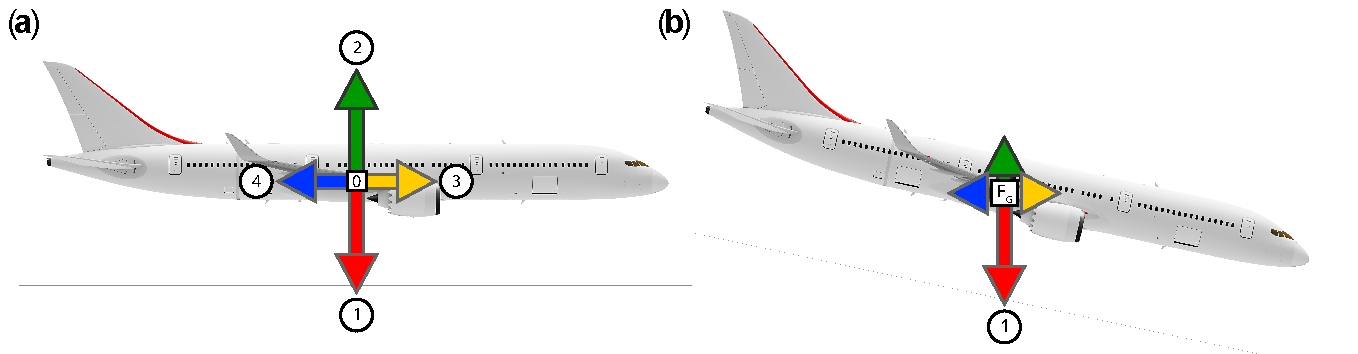
\includegraphics[width=\textwidth]{KraefteFlugzeug.pdf}
\caption[Wirkende Kr�fte am Flugzeug]{Wirkende Kr�fte am Flugzeug. \fa Normaler Flug bei konstanter H�he. \fb W�hrend der $0\,g$ Phase des Parabelflugs} 
\label{abb:bew_Parabelflug01}
\end{figure}
Um den Auftrieb auf Null zu bringen, erzeugt man durch das H�henruder des Flugzeugs einen negativen Anstellwinkel, der Schub kompensiert gerade noch den Luftwiderstand. 
Dynamisch sieht der Parabelflug wie folgt aus (\figref{bew_Parabelflug02}): 
Flugzeug fliegt mit $\SI{825}{\km\per\hour}$ in einer H�he von $\SI{6100}{\metre}$. Es beginnt dann einen Steigflug unter einem Winkel von ca. $45\degree$ f�r ca. $\SI{20}{\second}$ auf ca. $\SI{7600}{\metre}$ mit einer Beschleunigung von ca. $\SI{1.8}{\g}$. Nun wird das Flugzeug in den freien Fall (bzw. noch am Anfang \glqq Wurf\grqq{}) gebracht. Wir haben also eine Wurfparabel mit $v_0=$, $\alpha = 45\degree$, $h_0 = \SI{7600}{\metre}$. 
Die Scheitelh�he dieses Wurfes wird bei $h_\text{max} = \SI{8500}{\metre}$ mit einer verbleibenden Geschwindigkeit $v_\text{Top} = \sqrt{{v_\text{x}}^2+{v_\text{z}}^2}$ von $\SI{370}{\km\per\hour}$ erreicht, danach beginnt der freie Fall mit $\alpha=-45\degree$ f�r ca. $\SI{20}{\second}$ und bei einer H�he von $\SI{7600}{\metre}$ wird das Flugzeug \glqq angefangen\grqq{} um die normale Fluglage und Fluggeschwindigkeit wieder zu erreichen.
\begin{figure}[H]
\includegraphics[width=\textwidth]{Parabelflug.pdf}
\caption[Ablauf eines Parabelfluges]{Ablauf eines Parabelfluges} 
\label{abb:bew_Parabelflug02}
\end{figure}
\end {sol} 
%\href{PhysikUncut_Part1.pdf#prb:bew_Parabelflug}{\textcolor{blue} {$\rightarrow$ zur \probref{bew_Parabelflug}.}}\\
\textcolor{blue} {$\rightarrow$ zur} \probref{bew_Parabelflug}.\\
\noindent\rule[1ex]{\textwidth}{0.5pt}  \newpage


%%%-----------------------------------------------------------------------------------------------------------
%%%-----------------------------------------------------------------------------------------------------------


\subsection{�bungen zu beschleunigten Bezugssystemen}

%-----------------------------------------------------------------------------------------------------------
\hypertarget{lsg:bew_AbplattungPlaneten}{}
\begin{sol}{prob:bew_AbplattungPlaneten}\label{lsg:bew_AbplattungPlaneten}%�bung17
\textbf{Abplattung der Planeten} \\  \\
Der Einfachheit halber lassen wir die Striche f�r das System $\vec{\Sigma}'$ weg.
Wir bleiben ja ausschlie�lich im mitbewegten System. Au�erdem schreiben wir der K�rze wegen f�r die Umdrehungsfrequenz der Erde $\omega$ einfach $\omega$, analog f�r die Masse der Erde $M_\text{E}$ einfach $M$ und $R_\text{E}$ einfach $R$ f�r den mittleren Erdradius, sowie $g_0= GM/R^2$ f�r die mittlere Schwerebeschleunigung. Die Beziehungen sind dann auch direkt f�r andere Planeten anwendbar.

\begin{subprobs}
%--------------------------Aufgabenteil 1
%\subprob{�nderung der Schwerebeschleunigung durch die Zentrifugalkraft \\ -- Sph�rische Erde}
\subprob{�nderung der Schwerebeschleunigung durch die Zentrifugalkraft - Modell 0}\\
	\textbf{\textit{Modell 0: }} In diesem Modell wird die Erde (der Planet) als Kugel angenommen (quasi als ein starrer nicht verformbarer K�rper). Durch die Wirkung der Zentrifugalkraft kommt es aber zu einer Abweichung der Lotlinie, \dh der Richtung der Schwerebeschleunigung.\\
	Nach \figref{bew_Rot_Erde5} und Gleichung \eqref{eq:bew_effektives_g} gilt mit $\varphi$ als geographische Breite $g_\text{eff} = g_0 - R\,{\omega}^2\cos^2\varphi$
	und
	\begin{align}
		g'=& \sqrt{{g_\text{eff}^2+{b'_{\text{II}}}^2}} = \sqrt{{g_0}^2-2g_0\, R \,\omega^2\cos^2\varphi + {R}^2\,\omega^4\,\cos^4\varphi + {R}^2\,\omega^4\,\sin^2\varphi\,\cos^2\varphi} \nonumber \\
		=& g_0\sqrt{1+\frac{{R}^2\,\omega^4\,\cos^2\varphi}{g_0^2}\,\bigg[\cos^2\varphi+\sin^2\varphi-2\frac{g_0}{R \omega^2}\bigg]} 
		= g_0\sqrt{1+\frac{{R}^2\,\omega^4\,\cos^2\varphi}{g_0^2}\,\bigg[1-\frac{2g_0}{R\,\omega^2}\bigg]} \,. 
		\label{eq:bew_lsgAbplattung_a1}
	\end{align} 
Die Maximalwerte werden jeweils bei $\varphi = 90\degree$ (am Pol) und die Minimalwerte bei $\varphi = 0\degree$ (am �quator) erreicht, wie man unschwer an der Gleichung erkennt.\\
Interessant ist aber noch die Frage, wann die Abweichung zwischen $\vec{g_{eff}}$ und $\vec{g'}$ maximal wird.
Dies ist gleichbedeutend mit der Suche nach dem Maximum von $\tan\alpha = b'_\text{II} / g_\text{eff}$.
Wie man durch Differenzieren findet (siehe Nebenrechnung) ergibt sich
\begin{align*}
\alpha_\text{max} &=\arcsin\lk\frac{\frac{1}{2} R\,\omega^2}{g_0-\frac{1}{2} R\,\omega^2}\rk 
\qquad \text{bei} \qquad
\varphi_\text{max} =\arctan\sqrt{1-\frac{R\,\omega^2}{g_0}} \,.
\end{align*}
F�r $R\, \omega^2 \ll g_0$ ergibt sich $\varphi_\text{max} \approx 45\degree$ und $\alpha_\text{max}\approx R \omega^2 / {2g_0} = 0.0989\degree$ (siehe \mscr~\mlbewref{AbplattungPlaneten.m}). Wir werden sehen, dass diese Abweichung der Lotlinie nicht ganz korrekt ist, denn wir haben ja die Abplattung der Erde in unserem Modell vernachl�ssigt. 
\begin{nebenrechnung}{Nebenrechnung:}
		\begin{align*}
		    \tan \alpha = \frac{b'_\text{II}}{g_\text{eff}} = \frac{R{\omega}^2\cos\varphi\sin\varphi}{g_0 - R{\omega}^2\cos^2\varphi} ~\rightarrow~
				\frac{\d}{\d\varphi}\tan\alpha(\varphi) = \cos^2(\varphi)(g_0-R\omega^2\sin^2(\varphi))-g_0\,\sin^2\varphi-R\omega^2\cos^4(\varphi) = 0 \\
				\rightarrow~g_0-R\omega^2\sin^2\varphi =g_0\tan^2\varphi+R\omega^2\cos^2\varphi ~\rightarrow ~ g_0(1-\tan^2\varphi) = R\omega^2 ~\rightarrow ~\tan\varphi_\text{max} =\sqrt{1-\frac{R\omega^2}{g_0}}\,. % ~~ \text{mit} ~~ \varphi_\text{max} = \arctan\sqrt{1-\frac{R\,\omega^2}{g_0}} \, .
		\end{align*}
\end{nebenrechnung}

\newpage
	%--------------------------Aufgabenteil 2
	\subprob{Berechnung der Abplattung der Erde}
In dieser Teilaufgabe wollen wir die Abplattung der Erde aus den bekannten Messwerten $\omega, M, g_0$ und dem �quatorradius $R_\text{A}$ berechnen. Wir werden dazu verschiedene Modelle betrachten.
	\begin{enumerate} [a) ] 
		\item \textbf{ Modell 1 }\\
	
	  Im \textit{Modell 1} wird die Oberfl�che der Erde als \textit{�quipotentialfl�che}\index{�quipotentialfl�che} angenommen. Um eine stabile Oberfl�che zu erhalten, muss die potentielle Energie, die sich aus der Summe der Gravita\-tionskr�fte und der Zentrifugalkr�fte ergibt, entlang der Oberfl�che konstant sein. Andernfalls w�rde sich ja die als verformbar angenommene Oberfl�che ausgleichen wollen. Die Oberfl�che stellt sich dann senkrecht zu $\vec{F_\text{Z}} + \vec{F}_\text{G}$ \bzw zu $\vec{g}'$ (\figref{bew_lsg_Erdrot1}) ein.\footnote{Das ist �quivalent der Richtung der sogenannten \textit{Lotlinie}\index{Lotlinie} (engl. \textit{plumb line}), die man sich aus der Richtung eines aufgeh�ngten Bleigewichts im Unterschied zu einer in den Erdmittelpunkt gerichteten Linie vorstellen und entsprechend berechnen kann (siehe dazu Betrachtung im Aufgabenteil 1 und \cite{Mohazzabi2000}).}
		Die Tangente an einem Oberfl�chenpunkt ist dann logischerweise ebenfalls senkrecht zur Summe aus Gravitations- und Zentrifugalkraft.\\
%Der so definierte K�rper ist kein Rotationsellipsoid. 
	
		Wir betrachten einen Massepunkt $m$ auf der Erdoberfl�che. Wir nehmen zun�chst eine Geometrie eines Rotationsellipsoids an, in der Erwartung, dass die Form des sich einstellenden K�rpers einem solchen entspricht (\figref{bew_lsg_Erdrot2}). Dann k�nnen wir schreiben\footnote{Man muss hinsichtlich der Bezeichnung geographische Breite \index{Geographische Breite, engl. \textit{latitude}} $\varphi$ und geozentrische Breite \index{Geozentrische Breite, engl. \textit{declination}} $\psi$ aufpassen, in der Literatur wird das nicht immer einheitlich gehandhabt. Vgl.\ dazu auch \figref{bew_lsg_Erdrot1} und Kapitel 3 im Band II dieser Reihe. F�r die Kugel gilt nat�rlich $\varphi = \psi$.}: 
		\begin{align}
			x^2+z^2=r^2(\varphi)\,.
		\end{align}
		F�r die Zentrifugalkraft gilt:
		\begin{align}
			\vec{F}_\text{Z} = m \, \omega^2 \left(		\begin{array}{c}		x \\		0 \\		\end{array}		\right) \,. \label{eq:bew_lsgAbplattung01}
		\end{align}
		F�r die Gravitationskraft setzen wir an:
		\begin{align}
			\vec{F}_\text{G} = - \frac{G  M  m}{r^3}\left(		\begin{array}{c}		x \\		z \\		\end{array}		\right)\,. \label{eq:bew_lsgAbplattung02}
		\end{align}
		Das Modell nimmt hier an, dass die Gravitationskraft in Richtung des Mittelpunktes zeigt.
Das ist inkorrekt, da wir ja in Teilaufgabe 1 und in \kap{bew_Coriolis-Kraft} gesehen haben, dass die Gravitationskraft nicht mehr in Richtung Erdmitte zeigt.
		Wir wollen zun�chst dennoch mit dieser N�herung fortfahren, um zu sehen, wie weit wir kommen und wie weit das Ergebnis von der Realit�t abweicht.\\
    Ein Tangentenvektor an die Oberfl�che ist \zb gegeben durch (auch das ist nicht ganz korrekt nach oben Gesagtem):
		\begin{align*}
		\vec{t} = \left( 	\begin{array}{c} 		1 \\		z'	\end{array}		\right) =	\left(		\begin{array}{c}		1 \\ 		\D z / \D x  		\end{array}		\right)\,.
		\end{align*}
		F�r eine stabile Oberfl�che muss wie gesagt gelten:
		\begin{align}
		(\vec{F}_\text{G}+\vec{F}_\text{Z})\cdot \vec{t}= 0 \,, \label{eq:bew_lsgAbplattung03}
		\end{align}
		woraus 
		\begin{align}
		-\frac{G M}{(x^2+z^2)^{\frac{3}{2}}}\,(x+z\, z') + \omega^2 \,x  = 0\, \label{eq:bew_lsgAbplattung04}
		\end{align}
		folgt. Unter den gemachten (N�herungs-)Annahmen haben wir mit Gl. \eqref{eq:bew_lsgAbplattung04} eine Differentialgleichung $z'(x,x',z)$ erhalten, die die Oberfl�chenform z(x) der Erde beschreibt.\\
		Mit dem Ansatz $\hat q=x^2+z^2$ kann diese DGL in 
		\[-\frac{1}{2}G\, M \,\hat q'\,\hat q^{-\frac{3}{2}}+\omega^2 \,x = 0 \]
		�berf�hrt werden, die sofort integriert werden kann
		\begin{align}
		\frac{G \,M}{\sqrt{x^2+z^2}}+\frac{1}{2}\omega^2 \,x^2 = C = \frac{G \,M}{R_\text{P}} \,, \label{eq:bew_lsgAbplattung05}
		\end{align}
		 was man leicht durch Differenzieren nachrechnet. Hierbei haben wir die Integrationskonstante $C$ sinnvollerweise so gew�hlt, dass wir bei $x= 0$ f�r $z$ den Polradius $z = R_\text{P}$ erhalten.
    F�r die Oberfl�chenform $z(x)$ erhalten wir schlie�lich:
		\begin{align} 
		z(x)= R_\text{P} \sqrt{\lk \frac{\omega^2 \,R_\text{P}}{2 G \,M}\, x^2 - 1 \rk^{-2} -\frac{x^2}{R_\text{P}^2}} \,. \label{eq:bew_lsgAbplattung06}
		\end{align}
Offensichtlich ist \eqref{eq:bew_lsgAbplattung06} nur n�herungsweise eine Ellipsengleichung, die man eigentlich als L�sung erwartet h�tte. In \mscr{}~\mlbewref{AbplattungPlaneten.m} haben wir die Oberfl�chenform nach Gl. \eqref{eq:bew_lsgAbplattung06} und auch die Abweichung zu einer Ellipse numerisch berechnet.

\begin{figure}[H]
\includegraphics[scale=1]{Lsg_Erdrot1.pdf}
\caption[Richtung der Gravitationskraft]{Richtung der Gravitationskraft bei kugelf�rmigen und abgeplatteten Planeten.
Eingezeichnet sind die Gravitationskraft $\vec{F}_\text{G}$ und die Zentrifugalkraft $\vec{F}_\text{Z}$, sowie die aus beiden resultierende Kraft.
Im Fall des abgeplatteten Planeten ist im Bild die N�herungsannahme enthalten, dass die wesentliche Masse des Planeten in der N�he des Kerns konzentriert ist.
In der Realit�t w�rde aber die Richtung von $\vec{F}_\text{G}$ je nach Masseverteilung nicht unbedingt zum Erdmittelpunkt zeigen (gestrichelt gezeichnet), was zu einer weiteren Verkippung der Tangente f�hrt.} \label{abb:bew_lsg_Erdrot1}
\end{figure}

\begin{figure}
\centering
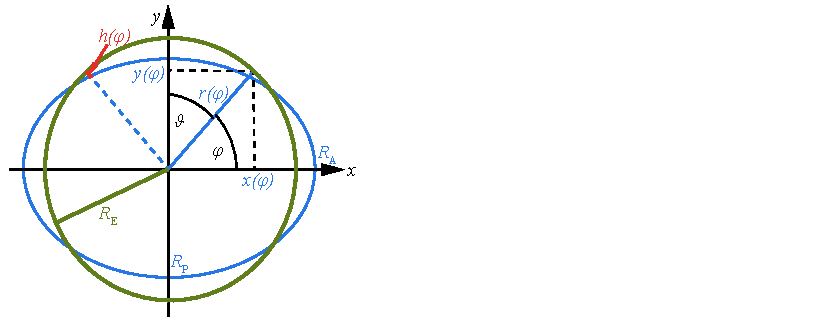
\includegraphics[scale=1]{Lsg_Erdrot2.pdf}
\caption{Geometrie der Abplattung} \label{abb:bew_lsg_Erdrot2}
\end{figure}

Wir wollen aus \eqref{eq:bew_lsgAbplattung05} nun das Verh�ltnis von Pol- zu �quatorradius ausrechnen, indem wir $z(R_\text{A})=0$ und $x=R_\text{A}$ setzen.
Wir erhalten dann aus \eqref{eq:bew_lsgAbplattung05}
	\begin{align} 
	1 +\frac{\omega^2}{2 G M}\, {R_\text{A}}^3 = \frac{R_\text{A}}{R_\text{P}} = \kappa \,. \label{eq:bew_lsgAbplattung07}
	\end{align}
	woraus der Polradius
	\begin{align} 
	R_\text{P} = \frac{R_\text{A}}{1+\frac{\omega^2}{2 G M} \, {R_\text{A}}^3} \label{eq:bew_lsgAbplattung08}
	\end{align}
folgt.
Die sogenannte \textit{Abplattung}\index{Abplattung} $f$ ist definiert als 
	\begin{align} 
	f = \frac{R_\text{A}-R_\text{P}}{R_\text{A}} = 1-\frac{R_\text{P}}{R_\text{A}} = 1-\frac{1}{\kappa} \,. \label{eq:bew_lsgAbplattung08a}
	\end{align}
In entsprechender N�herung gilt also f�r unser Modell 1 
	\begin{align}
	f_1 \approx 1- \lk 1-\frac{\omega^2}{2 G\,M}\, {R_\text{A}}^3 \rk  \approx \frac{\omega^2}{2\,G\,M}\, {R_\text{A}}^3 \approx \frac{3\omega^2}{8\pi\,G\,\varrho_\text{E}} \,. \label{eq:bew_lsgAbplattung_Modell01}
	\end{align}
Damit haben wir zun�chst das plausible Ergebnis, dass die Abplattung umso gr��er wird, je gr��er die Rotationsgeschwindigkeit und je kleiner die \anf{mittlere} Dichte wird.
Wenn wir allerdings die tats�chlichen Werte der Erde 
\begin{align*}
{R_\text{A}}^{\text{(exp)}} &= \SI{6378.137}{\km}\,,~M = \SI{5.974e24}{\kg}\,,\\
\omega &= \SI{7.292116e-5} {\per\second}\,,~ G = \SI{6.67384e-11}{\meter\cubed\kg\tothe{-1}\second\tothe{-2}} \,
\end{align*}
einsetzen, erhalten wir f�r den Polradius $R_\text{P}=\SI{6367.120}{\km}$ anstelle der tats�chlich gemessenen ${R_\text{P}}^{\text{(exp)}}=\SI{6356.752}{\km}$, also einen Unterschied der Radien von $\Delta R_1 =\SI{11.0}{\km}$ (im Unterschied zu den tats�chlichen $\Delta R^{\text{(exp)}} = \SI{21.4}{\km}$. Der nach Modell 1 ermittelte Polradius $R_{\text{P},1}$ ist also rund $\SI{10.4}{\km}$ zu gro� und damit erh�lt man mit
	\begin{align*}
		f_1 = 1:579.9  ~\quad \text{anstelle der gemessenen} ~\quad f^{\text{(exp)}} = 1:298.25\,,
	\end{align*}
auch eine deutlich zu geringe Abplattung.\\

%--------------------------Aufgabenteil 2b

\item \textit{\textbf{Modell 2}}\\
	   Wir wollen nun ein anderes Modell verwenden und betrachten dazu \figref{bew_lsg_Erdrot2}. In diesem \textit{Modell 2}
		 wollen wir die (rotierende) Erde als eine homogene Referenzkugel mit Radius $R$, Dichte $\rho_\text{E}$ und Masse $M=4\pi\varrho R^3/3$ plus einer infinitesimal d�nnen Schale mit positiver und negativer Masse auf $r=R$ mit einer Fl�chenmassendichte $\sigma(\theta)$ modellieren. Die d�nne Schicht beschreibt die  Massenumlagerung durch Abplattung und besitzt insgesamt ein \emph{Nullmasse}. Die resultierende Oberfl�che aus Kugel und Schicht sei wiederum eine geforderte �quipotentialfl�che des Gesamtpotentials.\footnote{Im Modell 1 hatten wir die Verformung einen rotierenden K�rpers (mit flexibler, fluider Oberfl�che) berechnet.) Die Gleichung \eqref{eq:bew_lsgAbplattung05} hatten wir als �quipotentialgleichung formuliert, wobei wir dort in guter N�herung das Gravitationspotential durch $-M g_\text{0} h(\varphi)= -M g_\text{0} h(\vartheta)$ ersetzt hatten. Wir k�nnten nat�rlich auch besser nach Aufgabenteil 1 $g_{\text{eff}}$ einsetzen, was die Rechnungen etwas verkompliziert, aber am Ergebnis nichts grunds�tzlich �ndert.} F�r die folgenden Rechnungen werden Grundkenntnisse der Potentialtheorie vorausgesetzt, wie wir sie in Band II und Band IV dieser Reihe im Detail behandeln. \\

Wir schreiben das Gesamtpotential als Summe von Gravitationspotential $U_\text{G}$ und dem Zentrifugalpotential $U_\text{Z}$, \dh $~U_{\text{tot}} = U_\text{G} + U_\text{Z}~$ und es 
gilt $~U_{\text{tot}}(\text{�quator})=U_{\text{tot}}(\text{Pol})~$. 
Mathematisch �quivalent zur Forderung an die �quipotentialfl�che ist die Bedingung, dass im Potential $U_\text{tot}$ auf der Oberfl�che kein
$\theta$-abh�ngiger Anteil verbleiben darf (zumindest bis zur betrachteten Ordnung).

Wir wollen eine kleine Abplattung annehmen ($\varepsilon  \ll 1$) und parametrisieren die Oberfl�che als ($\ell=2$-) Deformation �ber 
\begin{equation}
r_s(\vartheta)=R\lk 1+\varepsilon\,\PL2(\cos\vartheta)\rk \quad \text{worin}~~\PL2(\cos\vartheta)=\frac12(3\cos^2\vartheta-1) ~~\text{und} ~~|\varepsilon|\ll 1\,.
\end{equation}
Damit gilt
\begin{align}
		R_\text{P} &= r_s(\vartheta=0)=R\,(1+\varepsilon) \quad \text{und} \quad R_\text{A} = r_s\,\lk \vartheta=\frac{\pi}{2}\rk = R\,\lk 1-\frac{\varepsilon}{2}\rk\,.
\end{align}
F�r reale Abplattung ist \iA $R_\text{A}>R_\text{P}$, also $\varepsilon<0$. Die geometrische Abplattung $f$
liefert bis zur ersten Ordnung in $\varepsilon$:
\begin{equation}
		f_2=\frac{R_\text{A}-R_\text{P}}{R_\text{A}} =\frac{R\,(1-\varepsilon/2)-R\,(1+\varepsilon)}{R\,(1-\varepsilon/2)} \approx -\frac{3}{2}\varepsilon\,\quad\rightarrow\quad \varepsilon\approx -\frac{2}{3}\,f\,. \label{eq:f_eps}
\end{equation}
Wir berechnen nun das Gravitationspotential der Kugel plus der d�nnen Schale. Auf der Oberfl�che $r=r_s(\vartheta)=R\,(1+\varepsilon\,\PL2)$ entwickeln wir das Potential nach Ordnungen von $\varepsilon$:
\begin{equation}
		U_\text{G,K}(r_s,\vartheta)= -\frac{GM}{R\,\lk 1+\varepsilon\, \PL2(\cos\vartheta)\rk} \approx -\frac{GM}{R}\lk 1-\varepsilon\, \PL2(\cos\vartheta)\rk = -\frac{GM}{R}+\frac{GM}{R}\,\varepsilon\,\PL2(\cos\vartheta)\,.
\end{equation}
Der $\PL2$-Anteil daraus ist
\begin{equation}
		U_{G,K}^{(\ell=2)}(\vartheta)=\frac{GM}{R}\,\varepsilon\,\PL2(\cos\vartheta)\,. \label{eq:U02}
\end{equation}
Die d�nne Schale als Massenumlagerung mit der Gesamtmasse Null stellt als Masseverteilung einen Quadrupol dar. Ihre radiale Oberfl�chenabweichung von der Referenzkugel ist gegeben durch
\begin{equation}
		\delta r(\vartheta)=r_s(\vartheta)-R=R\,\varepsilon\,\PL2(\cos\vartheta)\,
\end{equation}
und ihre Fl�chenmassendichte ist
\begin{equation}
		\sigma(\vartheta)=\rho\,\delta r(\vartheta)=\underbrace{\rho R\,\varepsilon}_{\sigma_2}\,\PL2(\cos\vartheta) = \sigma_2\,\PL2(\cos\vartheta)\,.
\end{equation}
Da $\int \PL2\,\D \Omega=0$ ist, ist die Forderung Gesamtmasse Schale $=0$ erf�llt.
Wir bestimmen f�r die Massenverteilung $\sigma(\vartheta)$  auf der Oberfl�che das Multipolmoment mit $\ell=2$:
\begin{equation}
		M_2=\intsl \sigma(\vartheta)\,R{}^{4}\,\PL2(\cos\vartheta)\,\D\Omega  =\sigma_2\,R{}^4\intsl \PL2{}^2\,\D\Omega\,.
\end{equation}
Unter Ausnutzung der Orthogonalit�t der Legendre-Polynome 
\begin{equation}
		\int \PL\ell{}^2\,\D\Omega=\frac{4\pi}{2\ell+1} \quad\Rightarrow\quad \intsl \PL2{}^2\,\D\Omega=\frac{4\pi}{5}\,,
\end{equation}
folgt:
\begin{equation}
		M_2=R^4 \frac{4\pi}{5}\, \sigma_2\, =\frac{4\pi}{5}\rho \varepsilon\,R{}^5\,.
\end{equation}
Das �u�ere Potential eines reinen Quadrupol-Moments ($\ell=2$) lautet nach der Potentialtheorie (der Subskript S steht f�r Schale)
\begin{equation}
		U_{\text{G,S}}^{(\ell=2)}(R,\vartheta)= -\frac{G}{R{}^3}M_2 =-\frac{G}{R{}^3}\left(\frac{4\pi}{5}\rho \varepsilon\, R{}^5\right)\,\PL2 = -\frac{4\pi G\rho\, R{}^2}{5}\,\varepsilon\,\PL2(\cos\vartheta) 
		= -\frac{3}{5}\frac{GM}{R}\,\varepsilon\,\PL2(\cos\vartheta)\,. \label{eq:Ush2}
\end{equation}
Aus \eqref{eq:U02} und \eqref{eq:Ush2} folgt f�r den gesamter $\PL2$-Anteil des Gravitationspotentials
\begin{equation}
		U_{G}^{(\ell=2)}(\vartheta)(\vartheta)=U_\text{G,K}^{(\ell=2)} + U_\text{G,S}^{(\ell=2)} =\lk 1-\frac{3}{5}\rk \frac{GM}{R}\varepsilon\,\PL2(\cos\vartheta) =\frac{2}{5}\frac{GM}{R}\,\varepsilon\,\PL2(\cos\vartheta)\,.\label{eq:Ug2}
\end{equation}

Nun brauchen wir noch den $\PL2$-Anteil des Zentrifugalpotentials.
Das gesamte Zentrifugalpotential ist
\begin{equation}
		U_\text{Z}(\vartheta)=-\frac12\omega^2 r^2\sin^2\vartheta\,.
\end{equation}
Wir ben�tigen den $\PL2$-Anteil bei $r\approx R$.
Mit
\begin{equation*}
		\sin^2\vartheta = 1-\cos^2\vartheta ~~ \text{\bzw}~ \cos^2\vartheta=\frac{1+2\,\PL2(\cos\vartheta)}{3}~~\text{und}~~	\sin^2\vartheta=\frac{2}{3}\lk 1-\PL2(\cos\vartheta)\rk
\end{equation*} erhalten wir
\begin{equation}
		U_\text{Z}(\vartheta)= -\frac12\omega^2 R{}^2\,\frac{2}{3}\lk 1-\PL2(\cos\vartheta)\rk = -\frac{1}{3}\omega^2 R{}^2 + \frac{1}{3}\omega^2 R{}^2\,\PL2(\cos\vartheta) = -\frac{1}{3}\omega^2 R{}^2 + U_\text{Z}^{(\ell=2)}(\vartheta)\,. \label{eq:Uc2}
\end{equation}
Da die Oberfl�che eine �quipotentialfl�che sein muss, muss der
$\vartheta$-abh�ngige Anteil (also der gesamte Koeffizient von $\PL2$) des Gesamtpotentials
auf der Oberfl�che verschwinden, \dh
\begin{equation}
		U_{G}^{(\ell=2)}(\vartheta) + U_\text{Z}^{(\ell=2)}(\vartheta)=0\,.
\end{equation}
Mit \eqref{eq:Ug2} und \eqref{eq:Uc2} erh�lt man daraus
\begin{equation}
		\frac{2}{5}\frac{GM}{R}\,\varepsilon + \frac{1}{3}\omega^2 R{}^2=0 	\quad\rightarrow\quad \varepsilon = -\frac{5}{6}\frac{\omega^2R{}^3}{GM}\,. \label{eq:eps_result}
\end{equation}
%
Mit \eqref{eq:f_eps} folgt unter den getroffenen Annahmen, \dh homogene Kugel plus infinitesimal d�nne Massenschale und kleiner Abplattung aus der �quipotential-Bedingung in erster Ordnung nach unserem Modell 2 
f�r die Abplattung 
\begin{equation}
		f_2 \approx -\frac{3}{2}\varepsilon = \frac{5}{4}\frac{\omega^2R{}^3}{GM} \approx 1:231.95\,. \label{eq:bew_lsgAbplattung_Modell02}
\end{equation}
Wir haben eine gegen�ber dem Modell 1 (Gl. \eqref{eq:bew_lsgAbplattung_Modell01}) verbesserte L�sung (siehe Tabelle \ref{tab:bew_AbplattungenModelle}), die aber immer noch die Realit�t nicht vollst�ndig korrekt beschreibt. Die Abplattung nach diesem Modell ist um den Faktor 5/2 gr��er als im Modell 1, nun aber um \ca $\SI{6.5}{\km}$ zu gro�.
Die Abweichung liegt darin begr�ndet, dass wir die Erde als homogen angenommen hatten. 
Die Realit�t liegt zwischen dem homogenen Fall (Modell 2) und dem Modell 1, das als Modell eines K�rpers angesehen werden kann, bei dem die wesentliche Masse im Zentrum desselben konzentriert ist (deswegen konnten wir ja auch die Gravitationskraft noch im Wesentlichen in Richtung Erdmittelpunkt zeigend annehmen).\\
Tats�chlich ist die Erde aber mit $f=1/298.25$ kugel�hnlicher als unser Modell 2 hergibt, weil ihr Kern mehr als doppelt so dicht wie der Mantel ist. Dadurch f�llt die Fliehkraft weniger ins Gewicht. Diese gr��ere Dichte des Erdkerns k�nnte besser mit einem Zwei-oder Mehr-Schalen-Modell des Erdinneren ber�cksichtigt werden\footnote{Dieses Modell erkl�rt dann auch das beobachtete Schwerefeld im nahen Weltraum relativ gut. Feinere Erdmodelle der Geophysik unterteilen Kruste, Erdmantel und Erdkern je zweimal, womit man aber bereits an die Grenzen der Berechenbarkeit st��t (siehe auch \probref{bew_traegheitsmomente}).}, wobei man dann, um die Gravitationskraft korrekt zu ber�cksichtigen, �ber alle infinitesimalen Massenelemente der Erde integrieren muss. Alternativ kann man nat�rlich auch die hier f�r $\ell=2$ abgebrochene Reihenentwicklung des Potentials nach Kugelfl�chenfunktionen  mit $\ell = 3,4 \ldots$ fortsetzen. \\

	%---------------------------------Teil2c
\item \textit{\textbf{Modell 3}}\\
	   Wir wollen im \textit{Modell 3} das Modell 2 etwas allgemeiner behandeln, in dem wir den Erdk�rpers nun aus einer Referenzkugel und Schicht (mit Dicke $h(\vartheta)$)) bestehend betrachten.\footnote{Das Modell l�sst sich dann auch leicht auf inhomogene Massenverteilung verallgemeinern, wenn auch die Integration entsprechend schwierig wird.} Wir berechnen wieder die �quipotentialfl�che als Addition der Effekte der Gravitation der Kugel, der Zentrifugalkraft und der Gravitation von der d�nnen Schale. Letzteres stellt die eigentliche Komplexit�t dar, denn wir m�ssen ja das Volumenintegral �ber alle Massenelemente der Schale (oder eines entsprechenden beliebigen Zusatzk�rper) bilden.

Wir wollen zun�chst eine N�herungsform f�r die Dicke der Schicht ableiten. 
F�r die �quipotentialfl�che kann man n�herungsweise herleiten (siehe Gl. \eqref{eq:bew_effektives_g} in \kap{bew_Coriolis-Kraft}:
\begin{align}
	g_0 h(\vartheta) + \frac{\omega^2}{2}\, R^2 \, \sin^2\vartheta = \text{const} \quad \rightarrow \quad \hat C =  h(\vartheta)-\frac{\omega^2\, {R}^2 \,\sin^2\vartheta}{2 g_0}\,. \label{eq:bew_lsgAbplattung09} 
\end{align}
Um $\hat C$ zu bestimmen, machen wir die plausible Annahme, dass das Volumen des Rotationsellipsoids gleich dem der unverformten Kugel ist, d.h. es findet zwar eine Verformung, aber keine Kompression statt (man denke an eine Wasseroberfl�che oder ein fl�ssiges Plasma). Diese Bedingung ist gleichbedeutend mit 
\begin{align*}
	I &= \intsl\limits_{0}^{2\pi}\int\limits_{0}^{\pi}h(\vartheta)\,\sin\vartheta \,\,\D \varphi\, \D\vartheta = 2\pi \intsl\limits_{0}^{\pi}\lek\hat C +\underbrace{\lk\frac{\omega^2\,{R}^2}{2 g_\text{0}}\rk}_{\substack{\hat D}} \lk1- \cos^2\vartheta\rk\rek  \sin\vartheta \, \D \vartheta\,\nonumber \\
	 &=2\pi \,\lek-\hat C  \cos\vartheta - \hat D  \cos\vartheta + \hat D \frac{ \cos^3\vartheta}{3}\rek^{0}_{\pi} = 2\pi \,\lek\underbrace{+ 2\hat C + 2 \hat D - \frac{2}{3} \hat D}_{= 0}\rek \stackrel{!}{=} 0 \,. \nonumber
\end{align*}
Daraus folgt mit \eqref{eq:bew_lsgAbplattung09}
\begin{align}
	\hat C = -\frac{2}{3}\hat D = -\frac{\omega^2\,{R}^2}{3 g_\text{0}}  ~~\rightarrow~~h(\vartheta) = \frac{{R}^2\,\omega^2}{6 g_\text{0}}\,(3 \sin^2\vartheta-2)	\,.
\end{align}
Wenn man damit die Abplattung $f$ �ber $R_\text{A} = R + h(\vartheta=\pi/2), R_\text{P} = R + h(\vartheta=0)$ berechnet, ergibt sich wie erwartet der gleiche Wert wie f�r Modell 1 in Aufgabenteil 2a, n�mlich $f= \omega^2\,{R}^3/(2GM)$ (hier nur $R$ statt $R_\text{A}$), was aber keinen gro�en Unterschied macht.)\\
Wir wollen jetzt dieses H�henprofil $h(\vartheta)$ als Startwert verwenden und m�ssen zur Berechnung der Gravitationskraft der Schicht das Volumenintegral �ber alle Massenelement bilden. F�r jedes Massenelement gilt:
	\begin{align*}
			\D M = \varrho \,\D V = \varrho\,h(\vartheta) \,\D A = \varrho\,\beta(\gamma)\,(3 \sin^2\vartheta-2)\,R^2 \,\sin\vartheta\,\D \lambda \,\D \vartheta\,. 
	\end{align*}
Hier haben wir mit Gl \eqref{eq:bew_lsgAbplattung09} das H�henprofil in der $\vartheta$-Abh�ngigkeit unver�ndert gelassen, aber einen Korrekturfaktor  $\gamma>1$ eingef�gt. Dieser soll die aus den Richtungsabweichungen der Gravitationskraft resultierenden Effekte im Potential abbilden:
	\begin{align}
			h(\vartheta)=\beta(\gamma) \,(3 \sin^2\vartheta-2) ~~~\text{mit}~~~ \beta(\gamma)\,=\,\gamma\,\frac{R{}^2\,\omega^2}{6g_0} \,. \label{eq:ansatz_form}
	\end{align}
Aus der geometrischen Betrachtung von \figref{bew_lsg_Erdrot2} kann man ableiten, dass sich die Abst�nde f�r die Potentialberechnung $\text{Nordpol-Massepunkt auf der Oberfl�che}$ nach $d_1 = R\sqrt{2(1- \cos\vartheta)}$ \bzw $\text{�quator-Massepunkt}$ nach  $d_2 = R\sqrt{2(1- \sin\vartheta \,\cos\lambda)}$ berechnen. ($\lambda$ ist hier die Integrationsvariable L�ngengrad.)
Als spezielle Forderung einer �quipotentialfl�che fordern wir jetzt, dass das Gesamtpotential am �quator und den Polen gleich ist, was gleichbedeutend ist mit 
	\begin{align*}
   U_\text{tot}(\vartheta=0) &= (-2)\,g_0 \,\beta  + 0 - \intsl\limits_{0}^{\pi}\int\limits_{0}^{2\pi}\frac{G\,\varrho(\vartheta,\lambda)\,\beta\,(3 \sin^2\vartheta-2)}{R\sqrt{2(1- \cos\vartheta)}}{R}^2 \sin\vartheta\: \D\vartheta \,\D\lambda ~\\
	= U_\text{tot}(\vartheta=90\degree) & = (1)\,g_0 \,\beta  -\frac{m}{2} \omega^2 \ - \intsl\limits_{0}^{\pi}\int\limits_{0}^{2\pi}\frac{G\varrho(\vartheta,\lambda)\beta(3 \sin^2\vartheta-2)}{R\sqrt{2(1- \sin\vartheta\, \cos\lambda)}}{R}^2 \sin\vartheta\: \D\vartheta \,\D\lambda \,. 
\end{align*}
Hier nehmen wir nun eine \textit{homogene} Massenverteilung an, man k�nnte aber auch numerisch weiter mit $\varrho(\vartheta,\lambda)$ rechnen, um eventuell (bekannte) inhomogene Verteilungen mitzunehmen. Wir erhalten damit:
\begin{align}
	\gamma -1 = \gamma\intsl\limits_{0}^{\pi}\intsl\limits_{0}^{2\pi}\lek \frac{{R}^2}{4\pi R}(3 \sin^2\vartheta-2) \sin\vartheta\, \rek \, \lek\frac{1}{R\sqrt{2(1- \sin\vartheta \,\cos\lambda)}}-\frac{1}{R_\text{E}\sqrt{2(1- \cos\vartheta)}} \rek \,\D\lambda\,\D\vartheta\,, \label{eq:bew_gamma_abplattung}
\end{align}
woraus sich der Korrekturfaktor $\gamma$ �ber 
\begin{align}
	\gamma=1/(1-\mathcal{I})~\text{mit}~
	\mathcal{I}= \int\limits_{0}^{\pi}\int\limits_{0}^{2\pi}\frac{3 \sin^2\vartheta-2}{4\sqrt{2}\pi}\,\lk\frac{1}{\sqrt{1- \sin\vartheta \,\cos\lambda}}-\frac{1}{\sqrt{1- \cos\vartheta}}\rk \:\D\lambda\,\sin\vartheta \D\vartheta\,  \label{eq:bew_lsgAbplattung11}
\end{align}
berechnet. Dieses Integral k�nnen wir numerisch l�sen und erhalten $\gamma=5/2$ und damit $\Delta \text{R}=\SI{27.5}{\kilo\metre}$, also das gleiche Ergebnis wie in Teilaufgabe 2b) n�mlich im Vergleich zur Realit�t $\SI{21.4}{\kilo\metre}$ eine zu starke Abplattung von $\SI{6.1}{\kilo\metre}$. Das war auch zu erwarten, weil die Annahme einer homogenen Massenverteilung, wie wir sie im Schritt zu Gl.\eqref{eq:bew_gamma_abplattung} verwendet haben, wie wir gesehen haben ebenfalls nicht ganz korrekt ist.\\
Die Form nach dem Modell der so abgeplatteten Erde ist auch kein Rotationsellipsoid, wir hatten die Form ja mittels Gl. \eqref{eq:ansatz_form} in die Berechnung ``hinein gesteckt''. 

Man kann aber zeigen, dass man auch ohne eine Formannahme (wie in Modell 2 oder 3) f�r eine \textbf{homogene} Massenverteilung, das Problem allein aus der �quipotentialforderung f�r die Oberfl�che exakt l�sen kann\footnote{Siehe Zusatz�bung \probref{bew_abplattung_exakt} und \cite{Ledersteger1960}.}
 und dass dann die Form auch tats�chlich ein Rotationsellipsoid mit
\begin{align}
\frac{x^2}{R_\text{A}{}^2} + \frac{z^2}{R_\text{P}{}^2} = 1 ~~ \text~~ \eta = R_\text{A}/R_\text{P} = \frac{1}{\kappa}> 1
\end{align}
ist, wobei $\eta$ folgende Bedingung erf�llen muss:
\begin{align}
	(\eta^2+2)(\eta^2-1)^{-\frac{3}{2}}\arctan \sqrt{\eta^2-1}-\frac{3}{\eta^2-1} = \frac{{\omega}^2}{2 \pi \,G \,\varrho}=\frac{2\, R^3}{3\,G \,M}\,. \label{eq:bew_lsgAbplattung12}
\end{align}
Diese Gleichung l�sst sich numerisch l�sen und man findet mit $\varrho$ als mittlere Dichte der Erde die L�sung f�r das allgemeine Modell 3
	\[	\eta_3 = 1/\kappa_3 \approx 1.0043297 \,,\]
woraus eine geometrische Abplattung 
\begin{align}
f_3 = \frac{R_\text{A}-R_\text{P}}{R_\text{A}} \approx 1 - \eta \approx 1:230  \label{eq:bew_lsgAbplattung13}
\end{align}
folgt, was f�r die Erde nahe am Modell 2 liegt.\\

\textbf{\textit{Wissenschaftshistorischer Hinweis:}}\\
Die Bestimmung der Abplattung der Erde ist auch wissenschaftshistorisch au�erordentlich interessant, galt sie doch als eine der ersten Best�tigungen der Newtonschen Mechanik. So wurden 1733 und 1735 erste internationale (!) wissenschaftliche Expeditionen nach Equador und Lappland ausgesandt, um die Abplattung geod�tisch zu bestimmen. Diese Expeditionen waren die ersten gro�en \textit{Big Science} Projekte, noch vor der den gro�en Expeditionen zur Beobachtung des Venustransits und der Bestimmung der astronomischen Einheit in den Jahren 1761 und 1769, die wir in der Astrodynamik im Band II, Kapitel 3 behandeln werden. Ihr Budget entsprach damals ca. $0.1\%$ des franz�sischen Staatshaushalts. Wir empfehlen \cite {Greenstein2022} und die dort zitierte Literatur.

\end{enumerate}

	%--------------------------Aufgabenteil 3
\newpage
\subprob{Vergleich mit anderen Planeten}

Mit den L�sungen aus dem vorherigen Aufgabenteil k�nnen wir nun auch Absch�tzungen f�r die Gas\-planeten unseres Sonnensystems machen.
Wir benutzen Formel \eqref{eq:bew_lsgAbplattung08} f�r das Modell 1 des konzentrierten Kerns, welches die Differenz $\Delta R_1$ zwischen �quator- und Polradius ergibt, Formel \eqref{eq:bew_lsgAbplattung08} f�r das Modell 2 einer homogenen Massenverteilung (N�herung der Potentialtheorie mit $\ell=2$), woraus sich die Differenz $\Delta R_2$ ergibt, sowie Formeln \eqref{eq:bew_lsgAbplattung12} und \eqref{eq:bew_lsgAbplattung13} f�r die exakte Berechnung eines Rotationsk�rpers homogener Dichte. Wir vergleichen unsere Berechnungen mit den bekannten experimentellen Werten $f^{(\text{exp})}$ und $R^{(\text{exp})}$. \\

\begin{table}
\centering
    \hspace*{0.2cm}
    \begin{tabular}{L{1.25 cm}L{1.25cm}L{1.25cm}L{1.25cm}L{1.25cm}R{1.0cm}R{1.5cm}R{1.5cm}R{1.5cm}R{1.5cm}}
    Planet 	& $f_1$ & $f_2$ & $f_3$ & $f^{(\text{exp})}$ & $\gamma$ & $\Delta R_1$ & $\Delta R_2$ & $\Delta R_3$ & $\Delta R^{(\text{exp})}$ \\
    \noalign{\smallskip} \hline \noalign{\smallskip}
    Erde    & 579.88 & 231.95  &231.74  & 298.25 &  2.498 & \SI{11.0}{\kilo\metre} &  \SI{27.6}{\kilo\metre} &\SI{27.6}{\kilo\metre} &  \SI{21.4}{\kilo\metre} \\
    \noalign{\smallskip} 
    Jupiter & 23.76  & 9.10  & 9.48    & 15.41   &  2.684 & \SI{3141}{\kilo\metre} &  \SI{7852}{\kilo\metre}  &  \SI{7540}{\kilo\metre}  &\SI{4638}{\kilo\metre} \\
    Saturn  & 14.02  & 5.21  & 5.49    & 10.21   &  2.437 & \SI{4628}{\kilo\metre} &  \SI{11569}{\kilo\metre} &  \SI{10985}{\kilo\metre} &\SI{5904}{\kilo\metre} \\
    Uranus  & 66.84  & 26.34 & 26.74   & 43.62   &  2.462 & \SI{ 388}{\kilo\metre} &  \SI{970}{\kilo\metre}   &  \SI{ 956}{\kilo\metre}  &\SI{ 586}{\kilo\metre} \\
    Neptun  & 77.59  & 30.63 & 30.95   & 58.54   &  2.475 & \SI{ 323}{\kilo\metre} &  \SI{808}{\kilo\metre}   &  \SI{ 800}{\kilo\metre}  &\SI{ 423}{\kilo\metre} \\ 
    \noalign{\smallskip} \hline \noalign{\smallskip}
\end{tabular} 
    \hspace*{0cm}
		\caption[Vergleich der Ergebnisse der Abplattungsberechnungen f�r verschiedene Modelle und Vergleich zu den tats�chlichen Werten.]{Vergleich der Ergebnisse der Abplattungsberechnungen f�r verschiedene Modelle und Vergleich zu den tats�chlichen Werten. F�r die Erkl�rung der einzelnen berechneten Gr��en siehe Text. berechnet mit \mscr{}~\mlbewref{Abplattung.m}.}\label{tab:bew_AbplattungenModelle}
\end{table}

Man erkennt, dass auch bei den Gasplaneten der experimentelle Wert zwischen den Werten der beiden Modelle 1 und 2 liegt, wobei er im Gegensatz zur Erde deutlich dichter am Modell 1 des hochkonzentrierten Kerns liegt, was bei den Gasplaneten auch zu erwarten war. Saturn ist der am st�rksten abgeplattete Planet im Sonnensystem, w�hrend die Erde fast kugelf�rmig im Vergleich zu den Gasriesen ist. Man erkennt im Fall der Erde noch die relativ gute �bereinstimmung der Rechnung nach der Potentialtheorie (Modell 2) mit der exakten Berechnung f�r den Fall homogener Dichte (Modell 3), w�hrend bei den Gasriesen auf Grund von Dichte und Rotationsfrequenz gr��ere Abweichungen zu erkennen sind.

\end{subprobs}

\end{sol} 

%\href{PhysikUncut_Part1.pdf#prb:bew_AbplattungPlaneten}{\textcolor{blue} {$\rightarrow$ zur \probref{bew_AbplattungPlaneten}.}}\\
\textcolor{blue} {$\rightarrow$ zur} \probref{bew_AbplattungPlaneten}.\\
\noindent\rule[1ex]{\textwidth}{0.5pt}  \newpage


%-----------------------------------------------------------------------------------------------------------
\hypertarget{lsg:bew_Coriolis_I}{}
\begin{sol}{prob:bew_Coriolis_I}\label{lsg:bew_Coriolis_I}%�bung18
\textbf{Coriolis-Kraft I -- Ballistik}
\begin{subprobs}
\subprob{Exakte L�sung Freier Fall}
	Die Bewegungsgleichungen folgen aus \eqref{eq:bew_BGL_Erdrotation_Ko}:\:
	\begin{align}
	\ddot{x}(t) &= + 2\omega \sin \varphi \:\dot{y} \nonumber \\
	\ddot{y}(t) &= - 2\omega \sin \varphi \:\dot{x} - 2\omega \cos \varphi \:\dot{z} \nonumber \\
	\ddot{z}(t) &= + 2\omega \cos \varphi \:\dot{y} - g \,. \label{eq:lsg_BallistikCor1_1}
	\end{align}
	Einmalige Integration ergibt:
	\begin{align}
	\dot{x}(t) &= + 2\omega \sin \varphi \:y \nonumber \\
	\dot{y}(t) &= - 2\omega \sin \varphi \:x - 2\omega \cos \varphi \:z \nonumber \\
	\dot{z}(t) &= + 2\omega \cos \varphi \:y - g \,t\,. \label{eq:lsg_BallistikCor1_2}
	\end{align}
	Wir setzen $\dot{x}(t)$ und $\dot{z}(t)$ in die Gleichung f�r $\dot{y}(t)$ ein und erhalten die DGL
	\begin{align}
		\ddot{y} + 4\omega ^2 y = 2 \omega \,g \,\cos \varphi \:t \,,\label{eq:lsg_BallistikCor1_3}
	\end{align}
	deren L�sung durch
	\begin{align*}
		y(t) =  A\,\sin(2\omega\,t) + B\,\cos(2\omega\,t) + \frac{g\,\cos \varphi}{2 \omega} \,t \, , 
	\end{align*}
	gegeben ist. 
	Mit den Anfangsbedingungen $x(0) = y(0) = 0,~ \dot{x}(0) = \dot{y}(0) = \dot{z}(0) = 0$ und $z(0)= h$ folgt sofort $B=0$ und $A = -(g \cos\varphi)/(4 \omega^2)$.
        Die L�sung f�r die Ost-West-Richtung $y$ lautet also
	\begin{align}
		y(t) =  \frac{g \cos\varphi}{2 \omega} \lk t - \frac{\sin(2\omega\,t)}{2\omega} \rk \,.\label{eq:lsg_BallistikCor1_4}
	\end{align}
	Wir setzen nun $y(t)$ in die Gleichungen f�r $\dot{x}(t)$ und $\dot{z}(t)$ ein, integrieren und erhalten daraus mit den Anfangsbedingungen f�r die S�d-Nord-Richtung $x$
	\begin{align}
		x(t) =  g \sin\varphi \,\cos\varphi \,\lk \frac{t^2}{2} - \frac{1- \cos(2\omega\,t)}{4\omega^2} \rk \,,\label{eq:lsg_BallistikCor1_5}
	\end{align}
	\bzw f�r die H�he $z$
	\begin{align}
		z(t) = h - \frac{g \,t^2}{2} + g \cos^2\varphi \,\lk \frac{t^2}{2} - \frac{1-\cos(2\omega\,t)}{4\omega^2} \rk \,.\label{eq:lsg_BallistikCor1_6}
	\end{align}
	Damit haben wir das Problem exakt gel�st.
        F�r $\omega\,t \ll 1$ kann man die L�sung entwickeln
	\begin{align}
	x(t) &=  -\frac{g \sin\varphi \,\cos\varphi}{6} \,t^2 \, \lk\omega\,t\rk^2\,\nonumber \\
	y(t) &=   \frac{g \cos\varphi}{3} \,t^2 \,\lk\omega\,t\rk^2 \,.\nonumber \\
	z(t) &= h - \frac{g\, t^2}{2} + \frac{g}{6}\, \cos^2\varphi\,\, t^2 \,\lk\omega\,t\rk^2 \,.\label{eq:lsg_BallistikCor1_7}
	\end{align}
	F�r $(\omega\,t)^2 \approx 0$ geht dies in die N�herungsl�sung \eqref{eq:bew_BGL_Erdrotation_Lsg1} �ber. 
	Im \mscr~\mlbewref{BallistikCoriolis01.m} haben wir die L�sungen verglichen und auch den Fall eines sich sehr schnell drehenden Planeten berechnet.
        Man erkennt, dass die Corioliseffekte relativ gering sind und man \ia f�r den freien Fall gut mit der L�sung aus der St�rungsrechnung arbeiten kann.

\begin{figure}
\centering
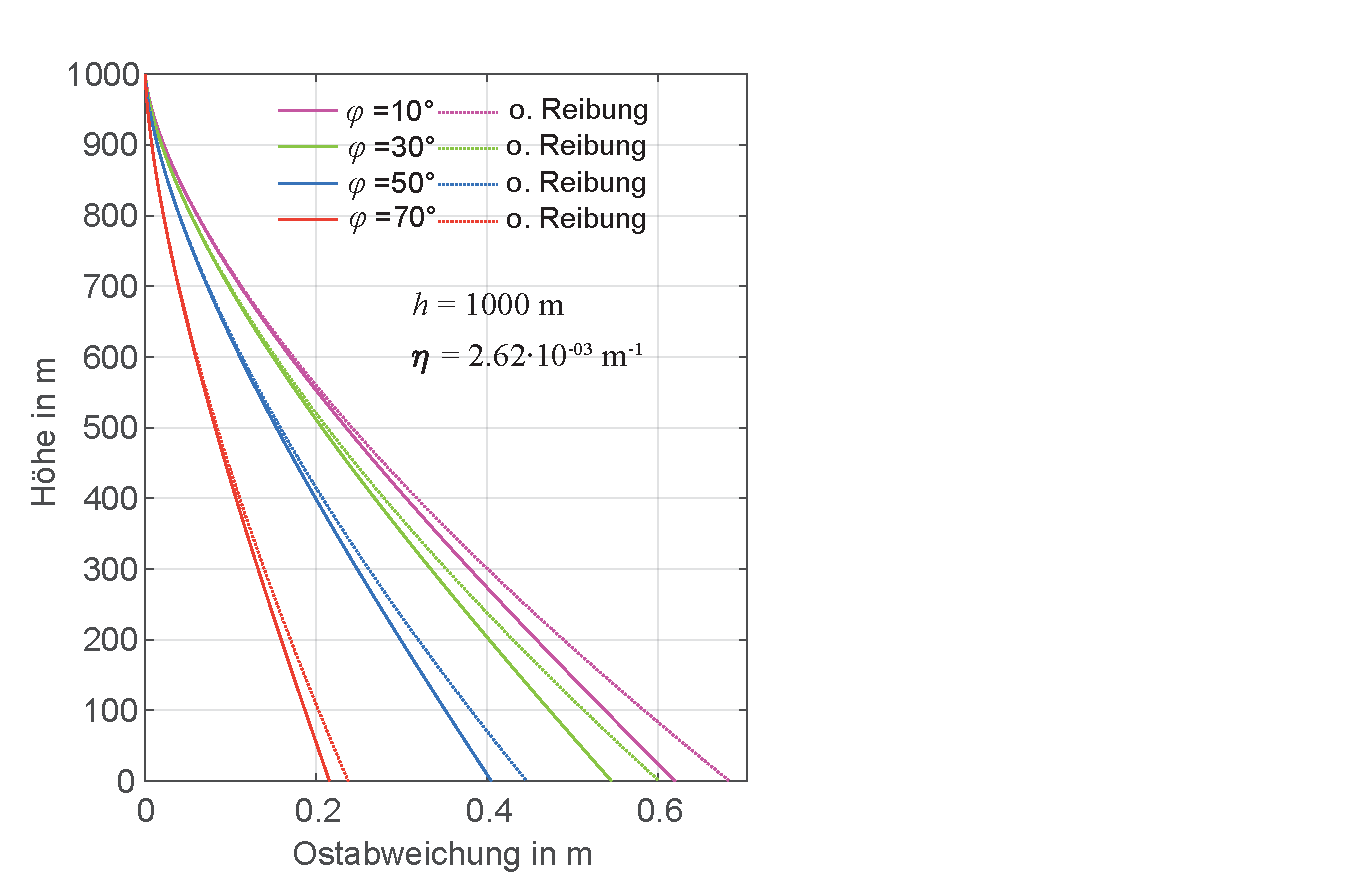
\includegraphics[width=0.8\columnwidth]{Lsg_Ballistik1.pdf}
\caption[Ostablenkung f�r den freien Fall einer Holzkugel]{Ostablenkung f�r den freien Fall einer Holzkugel von \SI{20}{\centi\metre} Durchmesser aus \SI{1000}{\meter} H�he mit und ohne Ber�cksichtigung der Luftreibung} \label{abb:bew_lsg_Ballistik1}
\end{figure}

\begin{figure}[H]
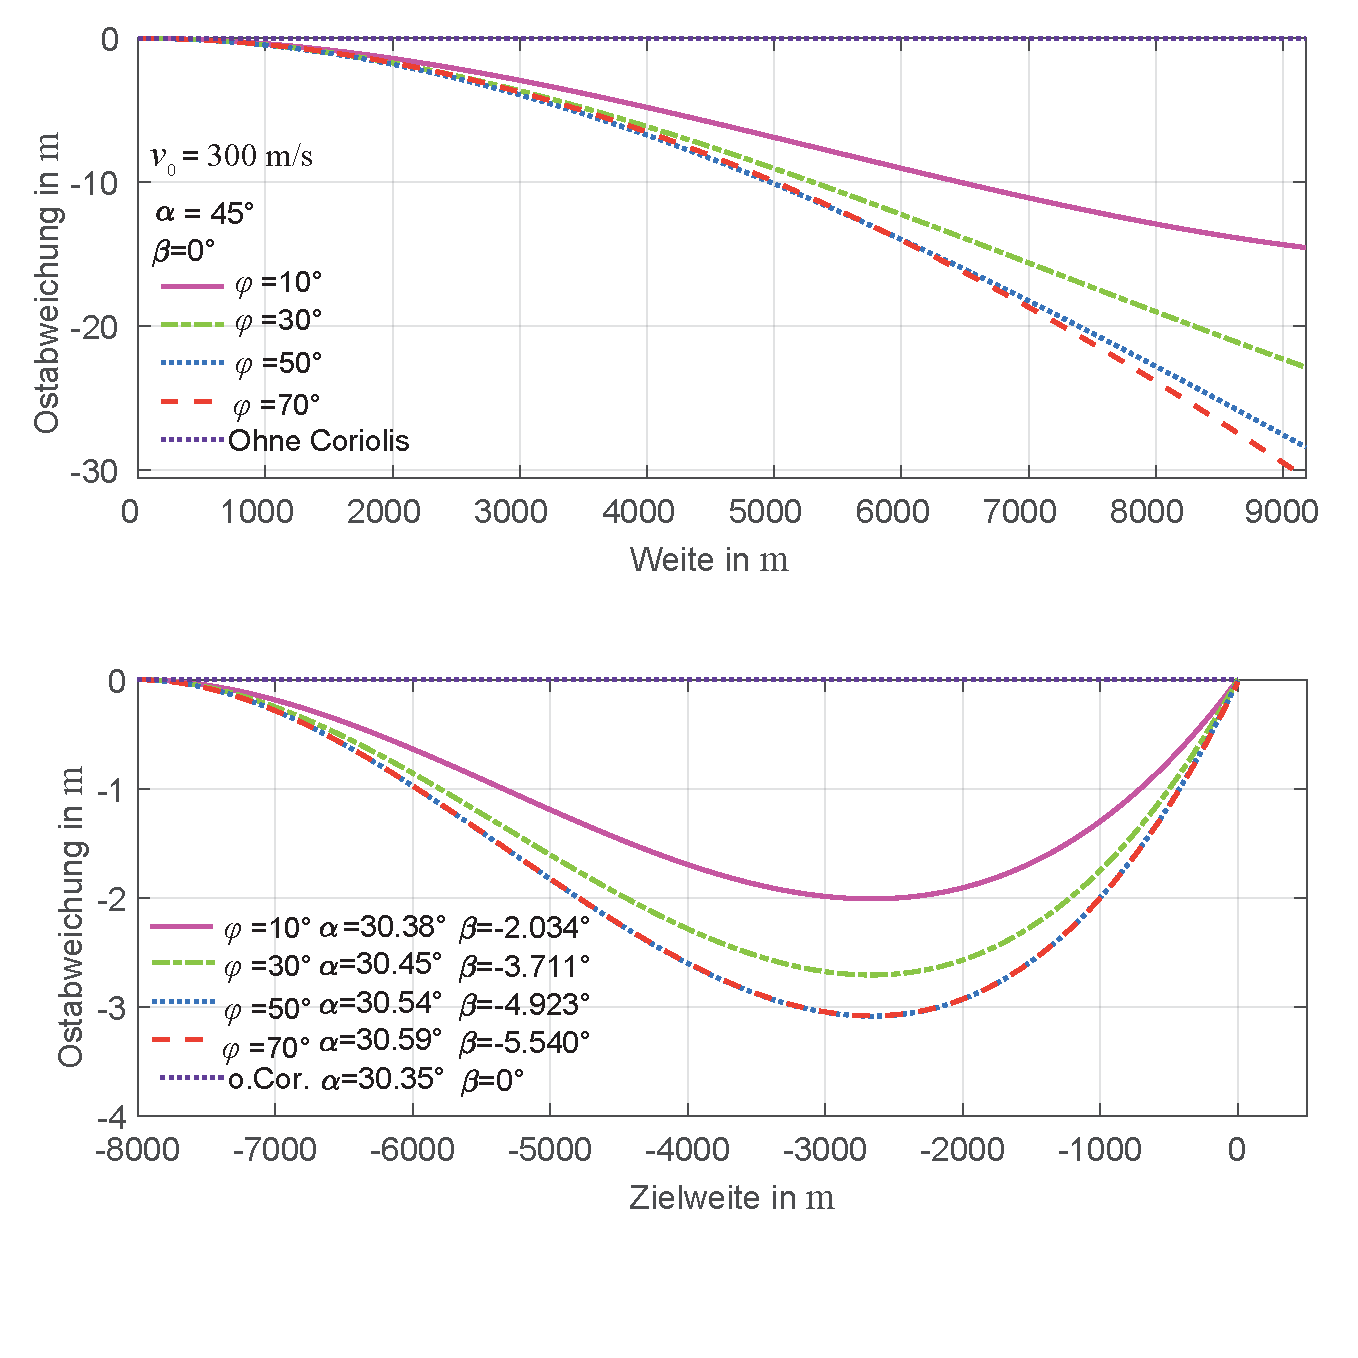
\includegraphics[width=0.75\columnwidth]{Lsg_BallistikCor_1.pdf}
\caption[Westablenkung eines nach S�den abgeschossenen Projektils]{Westablenkung eines mit $\SI{300}{\meter\per\second}$ nach S�den abgeschossenen Projektils f�r verschiedene geographische Breiten (oberes Bild) und Flugbahnprojektion auf die Horizontebene f�r einen Abschuss nach S�den mit eingestelltem Horizontal ($\alpha$)- und Vorhaltewinkel ($\beta$) um ein Ziel in 8000 m Entfernung zu treffen. Man beachte, dass negative Ostabweichung eine Westabweichung bedeutet} \label{abb:bew_lsg_BallistikCor_1}
\end{figure}

\begin{figure}[H]
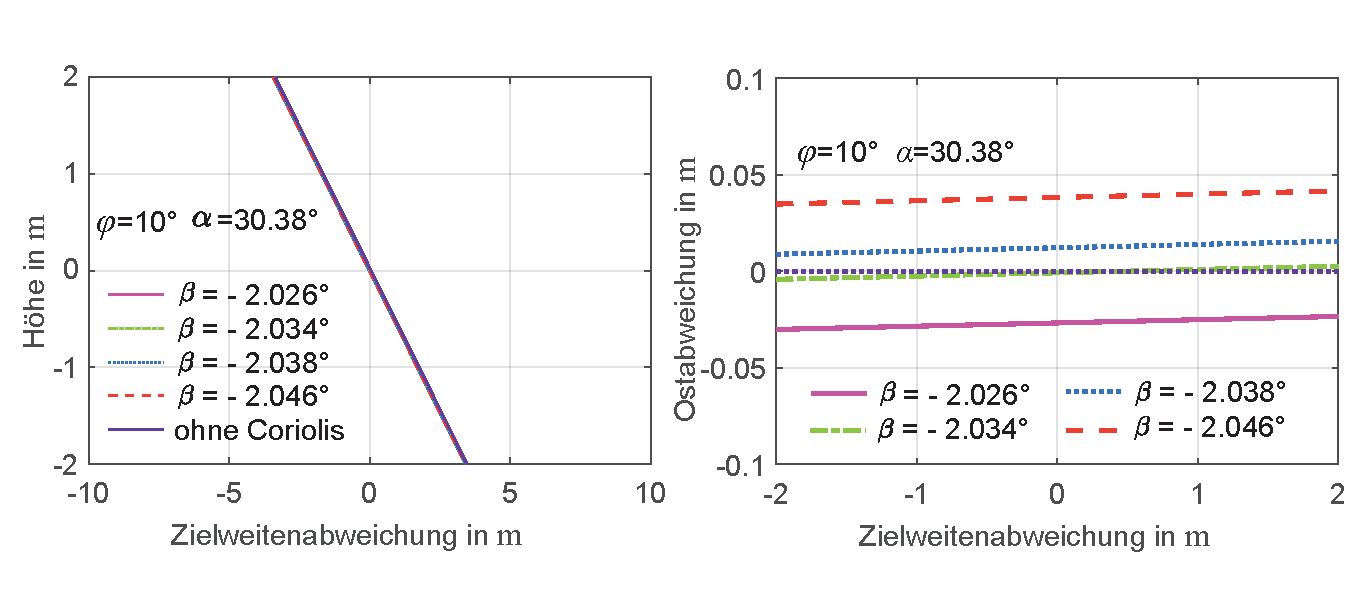
\includegraphics[width=\columnwidth]{Lsg_BallistikCor_2.pdf}
\caption[Verschiedene Vorhaltewinkel eines abgeschossenen Projektils]{Verschiedene Vorhaltewinkel eines mit $300 \:\mathrm{m/s}$ Richtung S�den abgeschossenen Projektils f�r eine geographische Breite von $\varphi = 10\degree$, um ein Objekt in 8000 m Entfernung zu treffen}\label{abb:bew_lsg_BallistikCor_2}
\end{figure}

\subprob{Exakte L�sung Ballistik} 

Die Bewegungsgleichungen lauten nun:
	\begin{align}
		\ddot{x}(t) &= + 2\omega \sin\!\varphi \:\dot{y} - \eta \,\dot{x} \,\lk \sqrt{\dot{x}^2+\dot{y}^2+\dot{z}^2} \rk^n \nonumber \\
		\ddot{y}(t) &= - 2\omega \sin\!\varphi \:\dot{x} - 2\omega \cos\!\varphi \:\dot{z} - \eta \,\dot{y} \,\lk \sqrt{\dot{x}^2+\dot{y}^2+\dot{z}^2} \rk^n \nonumber \\
		\ddot{z}(t) &= + 2\omega \cos\!\varphi \:\dot{y} - g - \eta \,\dot{z} \,\lk \sqrt{\dot{x}^2+\dot{y}^2+\dot{z}^2} \rk^n\,. \label{eq:lsg_BallistikCor2_1}
	\end{align}

Hierbei haben wir die Reibung mit dem Ansatz $- \eta \dot{x}_i^n$ ber�cksichtigt, aber offen gelassen, ob es sich um Stokes-Reibung ($ n=0 $) oder Newton-Reibung ($n=1$) handelt. 
F�r die Stokes-Reibung l�sst sich \eqref{eq:lsg_BallistikCor2_1} sogar exakt l�sen \cite{Neuberger1981}. 
Da in der Ballistik aber eher der Fall der Newton-Reibung relevant ist, werden wir diesen in Aufgabenteil 3 numerisch behandeln.
Zur L�sung f�r den reibungsfreien Fall $\eta=0$ leiten wir die Gleichung f�r $\ddot{y}$ aus \eqref{eq:lsg_BallistikCor2_1} noch mal nach der Zeit ab und erhalten:
\begin{align}
	\frac{\D^3}{\D t^3}{y}  &= - 4\omega^2 \,( \dot{y} \sin^2\!\varphi + \dot{y} \cos^2\!\varphi - 2\omega \,g \cos\!\varphi ) = - 4\omega^2 \,\dot{y} + 2\omega \,g \cos\!\varphi \nonumber \\
	\rightarrow \ddot{\zeta} + 4\omega^2 \,\zeta &= 2\omega \,g \cos\!\varphi \quad \text{mit} \quad \zeta = \dot{y} \,.\label{eq:lsg_BallistikCor2_2}
\end{align}
Die L�sung von \eqref{eq:lsg_BallistikCor2_2} ist gegeben durch
\begin{align}
	\zeta(t) = A\sin(2\omega\,t) + B\cos(2\omega\,t) + \frac{g \cos\!\varphi}{2\omega} \,. \label{eq:lsg_BallistikCor2_3}
\end{align}
Mit den Anfangsbedingungen $\zeta(0)=\dot{y}(0)=v_{0y}$ \bzw $\dot{\zeta}(0)=\ddot{y}(0) = -2\omega(\dot{x}(0) \sin\varphi + \dot{z}(0) \cos\varphi)$ bestimmen sich die Integrationskonstanten zu:
\begin{align}
	A &= -\lk\dot{x}(0) \sin\varphi + \dot{z}(0) \cos\varphi\rk = - (v_{0x} \sin\varphi + v_{0z} \cos\varphi) \nonumber \\
	B &=  v_{0y} - \frac{g \cos\varphi}{2\omega}\,. \label{eq:lsg_BallistikCor2_4}
\end{align}
Wir k�nnen \eqref{eq:lsg_BallistikCor2_3} noch mal integrieren und erhalten die L�sung f�r die Ost-West-Koordinate $y$ und analog f�r die anderen Koordinaten zu:
\begin{align}
	y(t) &= v_{0y}\,t + \frac{1}{2\omega} \lek A\, \lk 1- \cos(2\omega\,t) \rk - B\,\lk 2 \omega t-\sin(2\omega\,t) \rk \rek ~\,, \\
	x(t) &= v_{0x}\,t + \lek  A\, \lk t- \frac{\sin(2\omega\,t)}{2\omega} \rk + \frac{B}{2\omega} \lk 1 - \cos(2\omega\,t) \rk \rek \sin\varphi \nonumber \\ 
	& \ + g\,\cos\varphi\,\sin\varphi\,\frac{t^2}{2} ~\,, \\
	z(t) &= v_{0z}\,t - \frac{g}{2}\, t^2 + \lek  A\, \lk t- \frac{\sin(2\omega\,t)}{2\omega} \rk + \frac{B}{2\omega} \lek 1 - \cos(2\omega\,t) \rek \rek \cos\varphi \nonumber \\
	& \ + g\,\cos^2\varphi\,\frac{t^2}{2} \,.
 \label{eq:lsg_BallistikCor2_6}
\end{align}

F�r verschiedene geographische Breiten sind f�r einen Schuss in \figref{bew_lsg_BallistikCor_1} nach S�den unter $45\degree$ die erwarteten Abweichungen nach Westen aufgetragen.
Man erkennt, dass ein Ballistiker sehr wohl die Coriolis-Kraft ber�cksichtigen muss.
Die Effekte auf die H�he $z$ und die Schussweite $x_\text{max}$ sind dagegen Effekte der Gr��enordnung $(\omega \,t)^2$ und damit auf der Erde vernachl�ssigbar.
Wir stellen uns nun die Frage wie man die Schussrichtung w�hlen muss, damit man die Corioliseffekte ausgleicht.
Dazu muss man offensichtlich die Schussrichtung um einen Winkel $\beta$ nach Osten �ndern, um die Westablenkung zu kompensieren.
Die Schussweite ist n�herungsweise gegeben durch 
\begin{align}
	x_\text{max} \approx \frac{{v_0}^2\sin(2\alpha)\,\cos(\beta)}{g} = \SI{8000}{m} \,, \label{eq:lsg_BallistikCor2_7}
\end{align}
und die Westablenkung durch $y(t_\text{max})$ , worin $t_\text{max} \approx 2v_{0z}/g = 2 v_0 \sin\alpha$ die Flugzeit bis zum Auftreffpunkt ist.
Aus diesen beiden Gleichung lassen sich der  Winkel $\alpha$ gegen die Horizontale und der Richtungswinkel $\beta$ gegen die S�drichtung bestimmen.
In einer erster N�herung kann man dabei den Effekt der Winkel�nderung $\beta$ auf die Weite separieren.
Man bestimmt also zun�chst $\alpha$ aus \eqref{eq:lsg_BallistikCor2_7} mit dem Startwert $\beta = 0$, daraus dann aus \eqref{eq:lsg_BallistikCor2_6} mit $y(8000 \mathrm{m})=0$ numerisch den verbesserten Winkel $\beta'$ und wiederholt das bis eine hinreichende Genauigkeit erreicht ist.
Das Ergebnis ist in \figref{bew_lsg_BallistikCor_2} dargestellt, die Rechnungen sind in \mlbewref{BallistikCoriolis02.m} ausgef�hrt.

\begin{figure}[H]
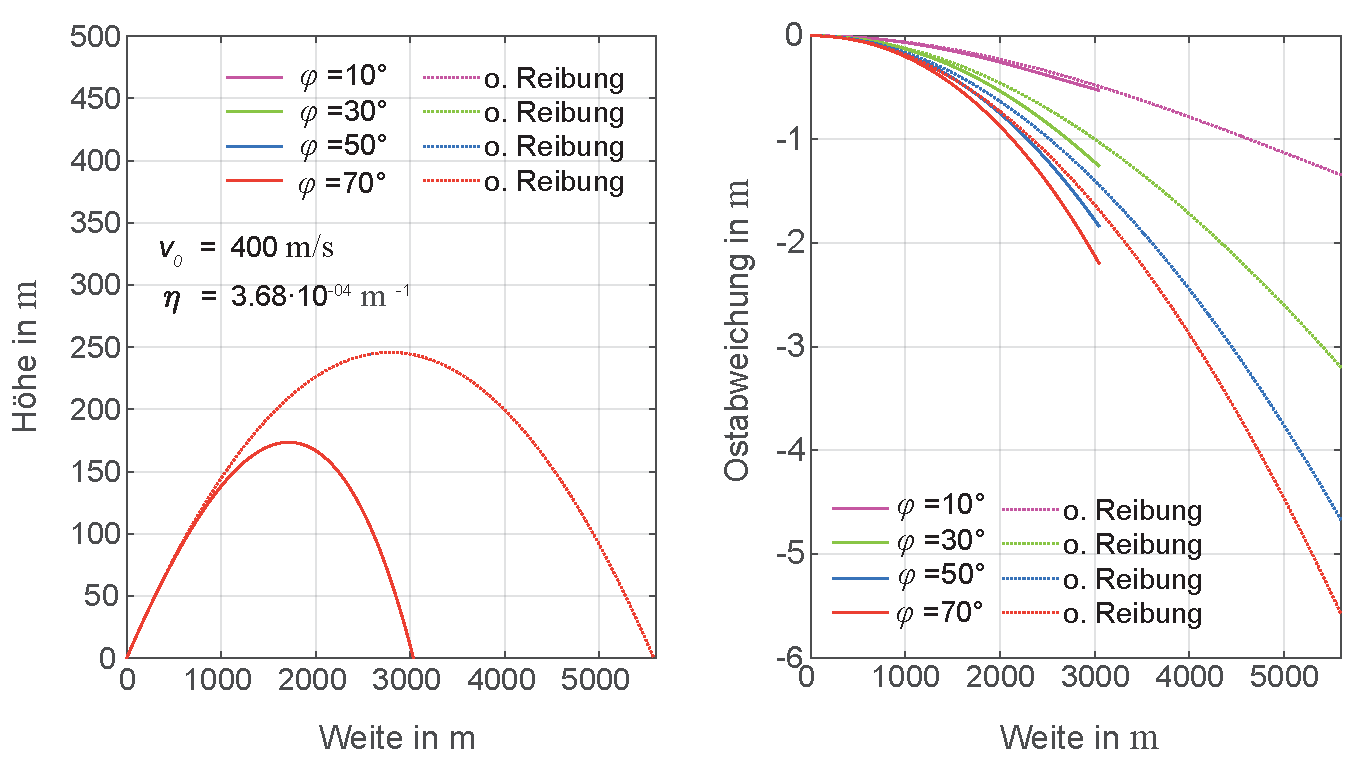
\includegraphics[width=\columnwidth]{Lsg_BallistikCor_3.pdf}
\caption[Flugbahn und Westablenkung einer abgeschossenen Kanonenkugel]{Flugbahn und Westablenkung einer mit $400 \mathrm{m/s}$ nach S�den abgeschossenen Kanonenkugel mit und ohne Ber�cksichtigung von Luftreibung bei verschiedenen geographischen Breiten (Horizontalwinkel $\alpha = 10\degree$)} \label{abb:bew_lsg_BallistikCor_3}
\end{figure}

\subprob{Numerische L�sung bei Reibung}
Wir wollen nun das DGL-System \eqref{eq:lsg_BallistikCor2_1} numerisch mit \matlab{} l�sen und zwar f�r den Fall der Luftreibung, die man gut mit der Newton-Reibung beschreiben kann:
\begin{align*}
	\eta = \frac{3}{4} \,c_\text{w} \,\frac{\varrho_\text{L}}{\varrho_\text{K}}\,\frac{1}{D_\text{K}} \,,
\end{align*}
worin $D_\text{K}$ der Durchmesser der Kanonenkugel ist.
Um das DGL-System numerisch mit der \matlab-Routine \odevf{} l�sen zu k�nnen, schreiben wir dieses um, in dem wir den Vektor $Y=(Y_1,Y_2,\ldots,Y_6)^\text{T}$ einf�hren, mit $Y_1 = x, Y_2 =\dot{x}, Y_3 = y, Y_4 = \dot{y}, Y_5 = z, Y_6 = \dot{z}$ Dann kann \eqref{eq:lsg_BallistikCor2_1} mit $v=\sqrt{\dot{x}^2+\dot{y}^2+\dot{z}^2} $ schreiben als:
\begin{align}
	\frac{\D}{\D t} \lk
	\begin{array} {c}
		 Y_1\\Y_2\\Y_3\\Y_4\\Y_5\\Y_6 
	\end{array} \rk
	= \lk \begin{array} {c}
		 \dot{x}\\ \ddot{x}\\ \dot{y}\\ \ddot{y}\\ \dot{z}\\ \ddot{z}
	\end{array} \rk
	= \lk \begin{array} {l}
		Y_2\\  2\omega\,\sin\!\varphi \:Y_4 - \eta\,v\:Y_2  \\ Y_4 \\ - 2\omega\,\sin\!\varphi \:Y_2 - 2\omega\,\cos\!\varphi \:Y_6 - \eta\,v\:Y_4 \\ Y_6 \\ 2\omega\,\sin\!\varphi \:Y_4 - g - \eta\,v\:Y_2 	\end{array} \rk \,.
\label{eq:lsg_BallistikCor3_1}
\end{align}

\newpage
Die Anfangsbedingungen sind f�r den freien Fall (Aufgabenteil 1) \bzw die Ballistik (Aufgabenteil 2) gegeben durch:
\begin{align*}
	Y_0 = \lk 	\begin{array} {c} 0 \\ 0 \\ 0 \\ 0 \\ h \\ 0	\end{array} \rk ~~~\text{\bzw}~~~~ Y_0 = \lk 	\begin{array} {c}  0 \\ v_\text{x0} \\ 0 \\ v_\text{y0} \\ 0 \\ v_\text{z0}  
	\end{array} \rk \,.
\end{align*}
%Der Funktionsaufruf f�r das DGL-System f�r die Routine \odevf{} lautet:\\
%\begin{lstlisting} [frame=single]
%% Differentialgleichungssystem f�r Coriolis-Kraft
%function dY = CoriolisDGLS(t,Y,Omeg,Cphi,Sphi,G,Eta)
  %dY    = zeros(6,1);
  %dY(1) = Y(4); dY(2) = Y(5); dY(3) = Y(6);
  %vbet  = sqrt(Y(4)^2+Y(5)^2+Y(6)^2);
  %dY(4) = 2*Omeg*Sphi*Y(5)-Eta*vbet*Y(4);
  %dY(5) = -2*Omeg*Sphi*Y(4)-2*Omeg*Cphi*Y(6)-Eta*vbet*Y(5);
  %dY(6) = 2*Omeg*Cphi*Y(5)-G-Eta*vbet*Y(6);  
%end
%\end{lstlisting} 
%\medskip
Das Ergebnis der Rechnungen ist in \figref{bew_lsg_BallistikCor_3} dargestellt und in \mlbewref{BallistikCoriolis03.m} im Detail hinterlegt.
Man erkennt, dass die Luftreibung sowohl die Schussweite als auch die Westablenkung reduziert.
Ein Ballistiker muss also beide Effekte und die geographische Breite ber�cksichtigen.



\end{subprobs}
\end{sol} 
%\href{PhysikUncut_Part1.pdf#prb:bew_Coriolis_I}{\textcolor{blue} {$\rightarrow$ zur \probref{bew_Coriolis_I}.}}\\
\textcolor{blue} {$\rightarrow$ zur} \probref{bew_Coriolis_I}.\\
\noindent\rule[1ex]{\textwidth}{0.5pt}  \newpage  


%-----------------------------------------------------------------------------------------------------------
\hypertarget{lsg:bew_Coriolis_II}{}
\begin{sol}{prob:bew_Coriolis_II}\label{lsg:bew_Coriolis_II}%�bung19
\textbf{Coriolis-Kraft II -- Fluss- und Schienenabtrag}

\begin{subprobs}
	\subprob{Flussabtrag}
	Ein gro�er Fluss str�mt im Mittel%
        \footnote{Wir nehmen hier nicht ganz richtig an,
        dass die Flie�geschwindigkeit �berall im Fluss
        gleich gro� ist.
        Wir werden sp�ter in \autoref{chap:kontmech} sehen,
        dass dies nicht der Fall ist.}
        mit $\dot{x}' = v' = - \SI{2}{\meter\per\second}$ nach Norden
        ($\varphi = 50\degree$ geographische Breite)
        und ist maximal $B = 2$ km breit.
        Die Coriolis-Beschleunigung in $y'$-(Ost)-Richtung ist dann $a_\text{Cor} = - 2 v' \omega \sin \varphi \approx 2.2 \, 10^{-4} \,\SI{}{\meter\per\second\squared} \approx 2.3\, 10^{-5}\: g$, also relativ klein.
        Coriolis- und Schwerebeschleunigung ergeben damit eine resultierende Beschleunigung, die normal zur Wasseroberfl�che sein muss. 
	Demzufolge steht die Wasseroberfl�che unter einem Winkel $\alpha$.
        Mit $\tan \alpha = H/B = a_\text{Cor}/g$ ergibt sich dann
		\[ H = \frac{- 2 B v' \omega \,\sin\varphi}{g} \approx \SI{4.5}{cm}\,.
	\]
Das Wasser eines 2 km breiten nach Norden flie�enden Stroms in Sibirien ($\varphi \approx 50 \degree $) kann also tats�chlich am �stlichen Ufer etwas h�her stehen als am westlichen.
Theoretisch w�re es also denkbar, dass sich der Fluss nach rechts mit der Zeit an das Ufer heranarbeitet.
Vorherrschende Winde aus West haben aber mindestens den gleichen Einfluss. 
\subprob{Schienenbeeinflussung}
Bei einem ICE ist $v_\text{max}' = 330$ km/h, die Schienenbreite der Normalspur betr�gt 1435~mm. Daraus ergibt sich in den gem��igten Breiten eine H�he $H$ von \ca 1.5~mm, was um etwa eine Gr��enordnung geringer ist als die Toleranzen bei der Gleisverlegung.
Jede noch so gro�e Kurve h�tte einen st�rkeren Effekt auf die unterschiedliche Abnutzung der beiden Schienen.
Es ist immer wieder erstaunlich, wie hartn�ckig sich die Mythen der Auswirkung der Coriolis-Kraft in solchen Effekten (auch Drehrichtung des abflie�enden Wassers im Waschbecken) �ber Generationen von Physikb�chern halten.
Vielleicht steckt dahinter der Wunsch, dass die Effekte der Physik doch offensichtlicher auftreten sollen.
Wir finden aber, dass gerade die Subtilit�t der physikalischen Effekte diese so interessant machen, ansonsten w�ren sie ja \anf{nichts Besonderes}.
\end{subprobs}

\end{sol} 
%\href{PhysikUncut_Part1.pdf#prb:bew_Coriolis_II}{\textcolor{blue} {$\rightarrow$ zur \probref{bew_Coriolis_II}.}}\\
\textcolor{blue} {$\rightarrow$ zur} \probref{bew_Coriolis_II}.\\
\noindent\rule[1ex]{\textwidth}{0.5pt}  \newpage  

%-----------------------------------------------------------------------------------------------------------
\hypertarget{lsg:bew_Coriolis_III}{}
\begin{sol}{prob:bew_Coriolis_III}\label{lsg:bew_Coriolis_III}%�bung20
\textbf{Coriolis-Kraft III -- Wetterph�nomene} \\ \\
Die Effekte der Coriolis-Kraft \eqref{eq:bew_Coriolis_Kraft}  wirken auch auf sich bewegende Luftmassen.
Die Bewegung von Luftmassen ist als Druckausgleich vom Hochdruck- zum Tiefdruck-Gebiet zu verstehen.
Tiefdruckgebiete entstehen beispielsweise dadurch, dass sich die Luft am Boden stark erhitzt und nach oben steigt.
\begin{subprobs}
	\subprob{Passatwinde}
	Luftmassen str�men zum relativ stabilen Tiefdruckgebiet entlang des �quators hin, d.h. es entsteht eine N-S-Bewegung auf der Nordhalbkugel \bzw eine S-N-Bewegung auf der S�dhalbkugel, wie in \figref{bew_ZyklonPassat}\,a dargestellt.
	In \eqref{eq:bew_BGL_Erdrotation_Ko} ist dann $\dot{x}' > 0$ und n�herungsweise $\dot{y}' = \dot{z}' = 0$, so dass es zu einer Kraft in West-Richtung $\propto - 2\omega \,\dot{x}' \,\sin{\varphi}$ kommt.
        Auf der S�dhalbkugel ist $\sin{\varphi} <0$, aber auch $\dot{x}' < 0$, so dass es wiederum zu einer West-Ablenkung kommt.
        Der resultierende Effekt sind die relativ stabilen Passatwinde.
	
\begin{figure}
\centering
\includegraphics[width=\textwidth]{ZyklonPassat.pdf}
\caption[Entstehung von Passatwinden und eines au�ertropischen Zyklons]{\fa Entstehung von Passatwinden \fb Entstehung eines au�ertropischen Zyklons auf der Nord- \bzw S�dhalbkugel (oberes \bzw unteres Bild)}\label{abb:bew_ZyklonPassat}
\end{figure}

\subprob{Zyklonen auf der Nord- und S�dhalbkugel}
	\begin{itemize}[a) ]
		\item Luftstr�mung vom Hoch zum Tief, Nordhalbkugel\\
	In der \figref{bew_LsgCoriolisIIIa} ist die Luftmassenbewegung vom Hoch- zum Tiefdruckgebiet auf der Nordhalbkugel dargestellt.
        Wenn sich die Luftmasse nach Norden bewegt, findet wegen der Coriolis-Kraft eine Ablenkung nach Osten, also aus Sicht der bewegten Luftmasse nach rechts statt.
        Entsprechend wird ein Wind, der von Westen auf das Tiefdruckgebiet zustr�mt, s�dlich abgelenkt.
        Aus Sicht der bewegten Luftmasse ist das wieder eine Rechtsablenkung.
        Da Winde immer von Hoch- zu Tiefdruckgebieten wehen, f�hrt diese Rechtsablenkung auf der Nordhalbkugel zu einer Drehung gegen den Uhrzeigersinn um das Zentrum des Tiefdruckgebiets.
        Zus�tzliche wird diese Drehung bei thermischen Tiefs im Zentrum noch durch den Aufstieg der warmen Luft nach oben �berlagert.
        Die resultierende Luftmassenbewegung kann eine entsprechende Spirale bilden.
        Damit haben wir das Entstehen von (au�ertropischen) Zyklonen auf der Nordhalbkugel beschrieben (Abb. oberes Bild in \figref{bew_ZyklonPassat}\,b).
        Die gleichen Effekte treten bei Hurrikans auf, bei denen das Tiefdruckzentrum bei ausreichender hoher Temperatur durch Verdunstung �ber der Meeresoberfl�che entsteht.

\begin{figure}[H]\centering
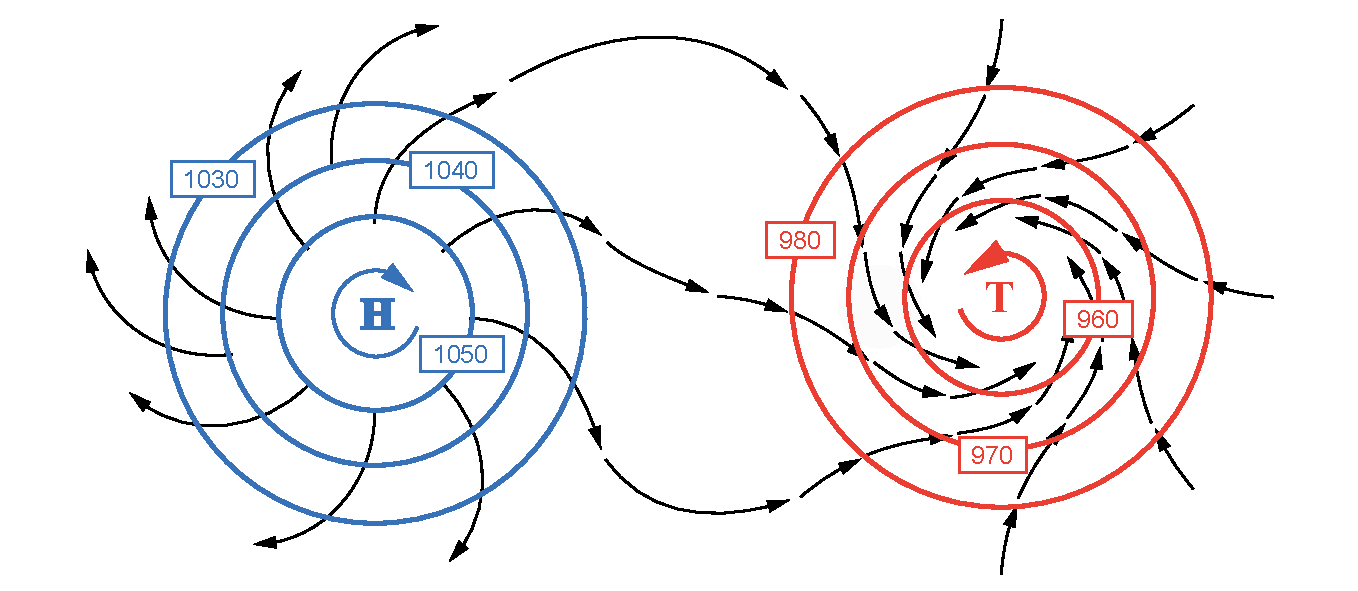
\includegraphics[width=\textwidth]{DruckausgleichHT01.pdf}
\caption[Druckausgleich zwischen Hoch- und Tiefdruckgebieten]{Druckausgleich zwischen Hoch- und Tiefdruckgebieten, die unser Wetter wesentlich beeinflussen. Dargestellt ist die Situation auf der Nordhalbkugel, wo die Luftmassen vom Hoch- zum Tiefdruckgebiet str�men und dabei nach rechts abgelenkt werden. Auf der S�dhalbkugel werden Sie entsprechend nach links abgelenkt (nicht dargestellt). Man beachte, dass diese Darstellung den Ausgleich am Boden zeigt}\label{abb:bew_LsgCoriolisIIIa}
\end{figure}

	\item Luftstr�mung vom Hoch zum Tief, S�dhalbkugel\\
	Auf der S�dhalbkugel wird die Luftmasse, die sich nach S�den bewegt �stlich abgelenkt, was gemessen in Windrichtung dann einer Linksablenkung entspricht.
        Auf der S�dhalbkugel f�hrt diese Linksablenkung dann zu einer Drehung im Uhrzeigersinn. (Abb. unteres Bild in \figref{bew_ZyklonPassat}\,b).

\begin{figure}[H]\centering
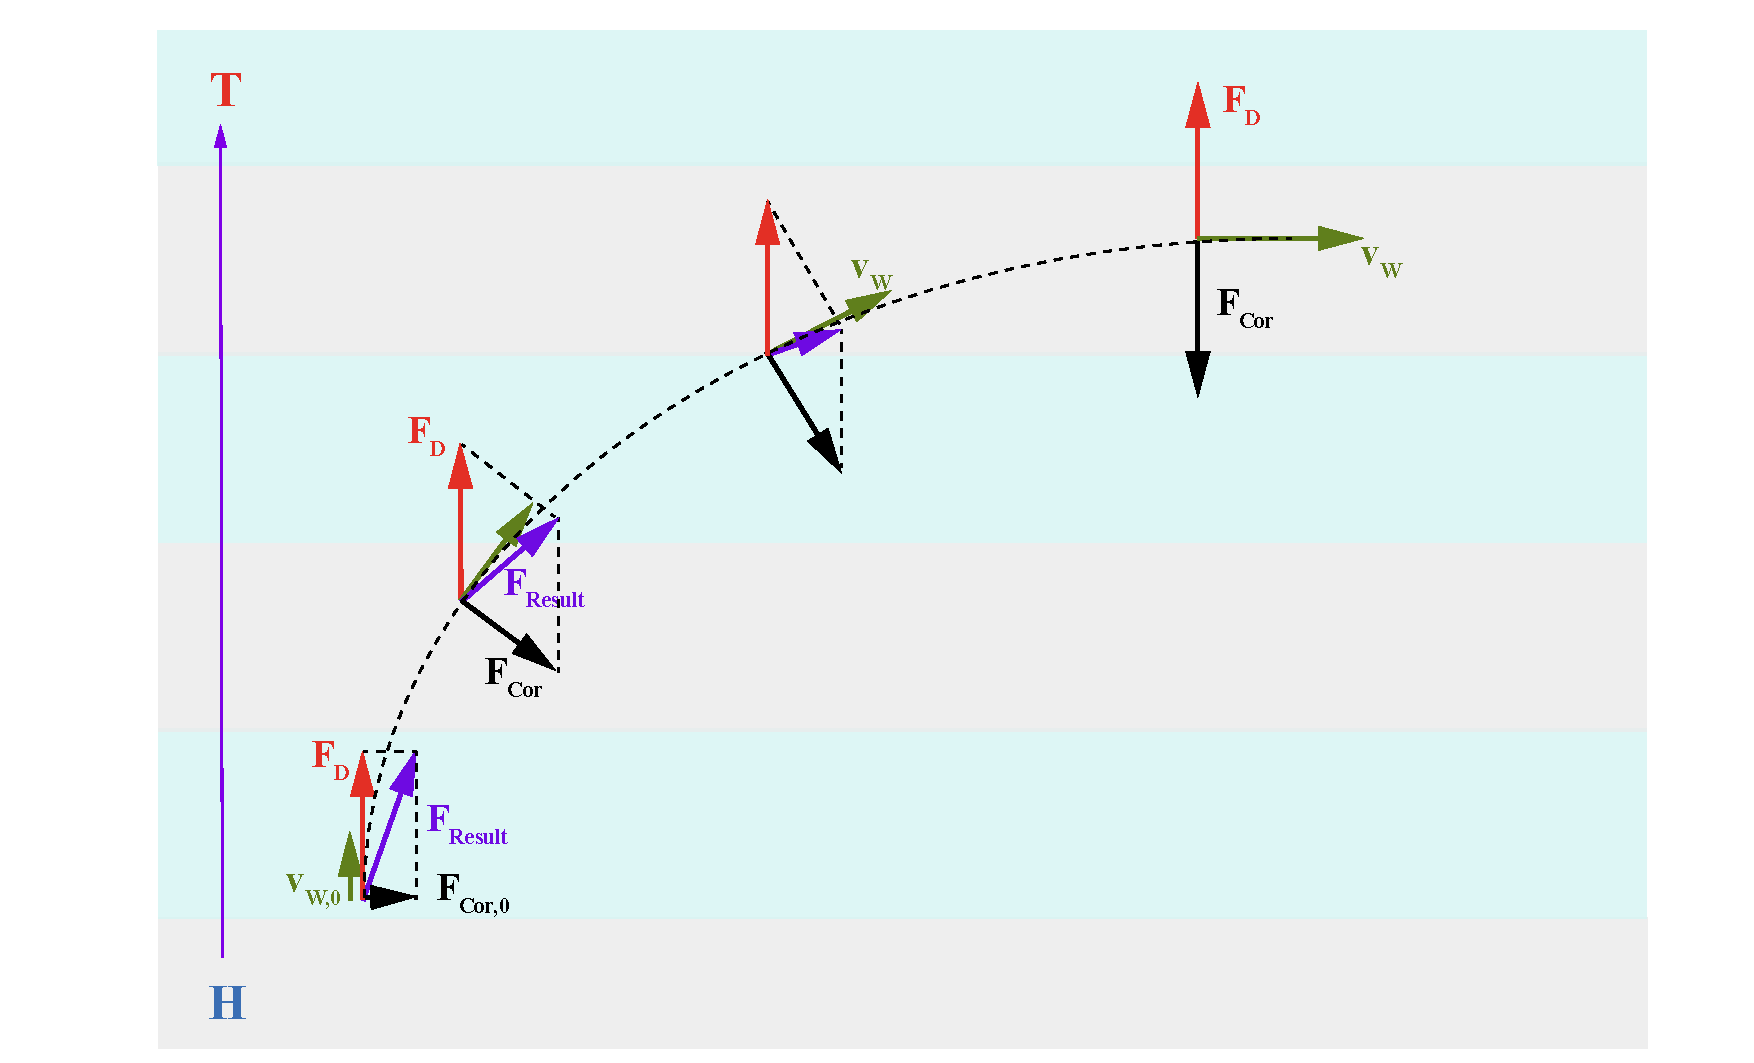
\includegraphics[width=\textwidth]{DruckausgleichHT02.pdf}
\caption[Einstellung der Windrichtung und Windgeschwindigkeit]{Einstellung der Windrichtung und Windgeschwindigkeit durch Zusammenwirkung von Druckgradientenkraft und Coriolis-Kraft auf der Nordhalbkugel nach \cite{Brauner2019}. Bei dieser Darstellung haben wir die Reibung, die unweigerlich am Boden auftritt, vernachl�ssigt. Man kann sich leicht �berlegen, dass diese dazu f�hrt, dass der station�re Geschwindigkeitsvektor nicht genau senkrecht auf dem Druckgradienten steht. die hier gezeigte Darstellung entspr�che also in etwa den Verh�ltnissen in einer H�henstr�mung }\label{abb:bew_LsgCoriolisIIIb}
\end{figure}

	\end{itemize}

\subprob{Windrichtung/-st�rke in Nordschottland und in Deutschland}
Um die Windrichtung und Windgeschwindigkeit zu berechnen, betrachten wir \figref{bew_LsgCoriolisIIIb}. 
Senkrecht zu den Isobaren wirkt durch den Druckgradienten die so genannte Druckgradientenkraft $\vec{F}_\text{D}$, die die Luftmassen in Bewegung setzt.
Diese werden durch die Coriolis-Kraft $\vec{F}_\text{Cor}$ nach rechts abgelenkt.
Station�res Gleichgewicht und damit die stabile Ausbildung einer Windrichtung ist dann gegeben, wenn die Coriolis-Kraft genau entgegengesetzt gleich der Druckgradientenkraft ist.
Dann str�mt der Wind in etwa parallel zu den Isobaren.
Wir k�nnen die Windgeschwindigkeit durch folgende �berlegungen absch�tzen.
Der Luftdruckunterschied $\Delta p$ �ber eine Distanz $\Delta s$ erzeugt auf ein Querschnittsfl�che $A$ und damit auf ein kleines Luftvolumen $A \Delta s$ eine Druckgradientenkraft mit einem Betrag von:
\begin{align*}
	F_\text{D} = \lk \frac{\Delta p} {\Delta s}\rk  A  \Delta s~.
\end{align*}
Wir betrachten nun ein Luftvolumen der Masse $\Delta m = \varrho_\text{L} A \Delta s$, 
welches sich mit der Geschwindigkeit $v$ in der geographischen Breite $\varphi$ bewegt.
Der Betrag der Coriolis-Kraft, der auf dieses Luftvolumen wirkt, ist
\begin{align*}
	F_\text{Cor} = 2 \Delta m \,\omega \,v \,\sin\varphi= 2 \omega \,v \,\sin\varphi \,\varrho_\text{L}\,A\,\Delta s~.
\end{align*}
Gleichsetzen von $F_\text{D}$ und $F_\text{Cor}$ und umstellen nach $v$ ergibt:
\begin{align}
	v = \frac{1}{2 \varrho_\text{L} \,\omega \,\sin\varphi} \frac{\Delta p}{\Delta s}\,. \label{eq:bew_Windgeschwindigkeit}
\end{align}
Der H�henwind (auch geostrophischer Wind genannt) ist also von der Dichte der Luft $\varrho_\text{L}$, der geographischen Breite $\varphi$ und dem Isobarenabstand $\Delta p / \Delta s$ abh�ngig.\footnote{Dieser so berechnete Wind kann in Bodenn�he durch Reibungseffekte auf etwa 2/3 sinken und auch in seiner Richtung ver�ndert werden.}

Im gegebenen Beispiel weht der Wind �ber Nordschottland vom Hochdruckgebiet �ber den Azoren kr�ftig in Richtung Osten bis Nordosten.
Die Windrichtung ist definiert als Herkunftsrichtung eines Windes, also sprechen wir hier von einem Westwind \bzw S�dwestwind. 
In Mitteleuropa ist der Wind wegen der geringen Luftdruckunterschiede sehr schwach.
Allgemein gilt: je gr��er der Abstand der Isobaren, desto geringer die Windgeschwindigkeit.
Und im Umkehrschluss: je geringer der Abstand der Isobaren, desto gr��er die Windgeschwindigkeit. 
\end{subprobs}

\end{sol} 
%\href{PhysikUncut_Part1.pdf#prb:bew_Coriolis_III}{\textcolor{blue} {$\rightarrow$ zur \probref{bew_Coriolis_III}.}}\\
\textcolor{blue} {$\rightarrow$ zur} \probref{bew_Coriolis_III}.\\
\noindent\rule[1ex]{\textwidth}{0.5pt}  \newpage 

%-----------------------------------------------------------------------------------------------------------
\hypertarget{lsg:bew_Coriolis_IV}{}
\begin{sol}{prob:bew_Coriolis_IV}\label{lsg:bew_Coriolis_IV}%�bung21
\textbf{Coriolis-Kraft IV -- Karussell} \\ \\
Die wirkenden Kr�fte auf einen bewegten K�rper sind in \figref{bew_Lsg_Scheibe01} dargestellt.

\begin{figure}[H]\centering
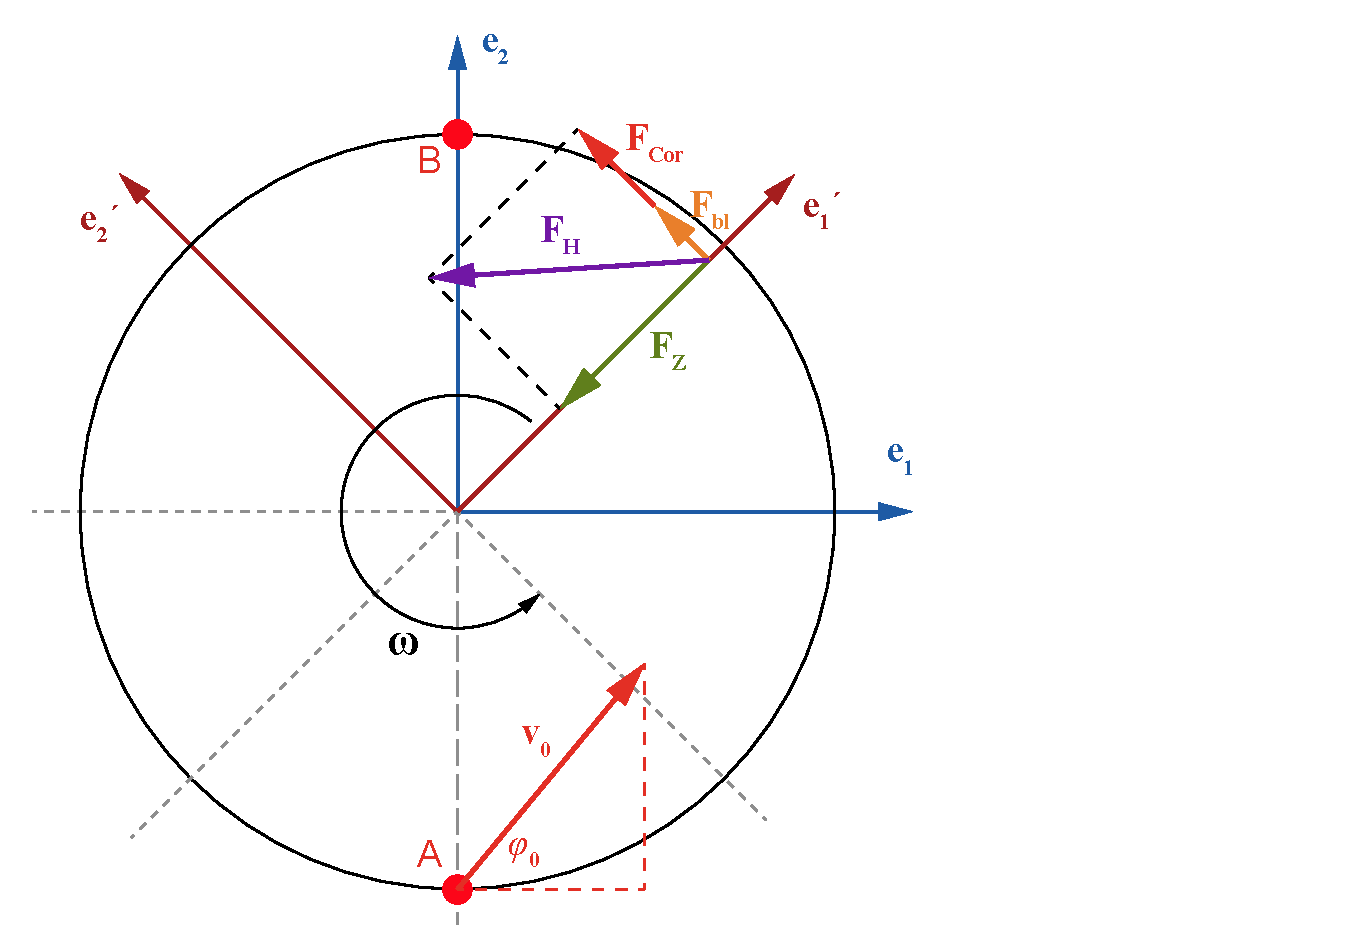
\includegraphics[width=0.8\textwidth]{Lsg_Scheibe01.pdf}%
\caption[Kr�fte auf einen bewegten K�rper auf einem sich drehenden Karussell]{Kr�fte auf einen bewegten K�rper auf einem sich drehenden Karussell. Angegeben sind die Tr�gheitskr�fte $\vec{F}_\text{Z}',\vec{F}_\text{Cor}',\vec{F}_\text{br} $, worin $\vec{F}_\text{br}$ die Euler-Kraft ist. Ebenso eingezeichnet ist die Haftreibungskraft $\vec{F}_\text{H}$ und die Richtung der Anfangsgeschwindigkeit $\vec{v}_0$ des K�rpers}
\label{abb:bew_Lsg_Scheibe01}
\end{figure}

\begin{subprobs}
\subprob{Haftreibung des Reifens}
Die Bewegungsgleichung in vektorieller Form lautet:
	\begin{align}
			m \,\ddot{\vec{r}}' &= \vec{F}_\text{R} -m\,\vec{\omega}'\times[\vec{\omega}'\times\vec{r}']-2m \,\vec{\omega}'\times\vec{v}'-m\,\dot{\vec{\omega}}\times\vec{r}' \,, \nonumber \\
		&=	\vec{F}_\text{R}+\vec{F}_\text{Z}'+\vec{F}_\text{Cor}' + \vec{F}_\text{br} \,, \label{eq:bew_lsg_Karussell_1}
	\end{align}
worin $\vec{F}_\text{R}$ die Reibungskraft ist, die durch die Reifen auf der Unterlage des Karussells aufzubringen ist.
Da sich das Go-Kart gleichf�rmig mit $v_0$ bewegen soll, muss die dazu notwendige Motor- \bzw Bremskraft ebenfalls �ber die Reibung auf den Boden des Karussells vermittelt werden.
Wir wollen nun die einzelnen Kraft-Komponenten bestimmen.
Aus der vektoriellen Zerlegung nach \figref{bew_Lsg_Scheibe01} ergibt sich ($\vec{\omega}$ zeigt aus der Bildebene heraus):
	\begin{align}
			m \,\ddot{\vec{r}}' &= 0 \,, \nonumber \\
			\Rightarrow \vec{F}_\text{R} &= m \,\vec{\omega}' \times\lk\vec{\omega}'\times\vec{r}'\rk+2m\,\lk\vec{\omega}'\times \dot{\vec{r}}'\rk+m\,\lk\dot{\vec{\omega}}'\times\vec{r}'\rk \,. \label{eq:bew_lsg_Karussell_2}
	\end{align}
Wir k�nnen die Kraft in die Komponenten der Achsen des mitbewegten KOS zerlegen und erhalten f�r:
	\begin{align*}
		\vec{F}_\text{R,1} &=  -m\,\omega'^2 \,r' \:\vecpeX \,,\\
		\vec{F}_\text{R,2} &= +2m\,\omega'\,v'\:\vecpeY + m\,\dot{\omega}'\,r'\:\vecpeY \,.
	\end{align*}
Die Coriolis-Kraft und die Euler-Kraft zeigen also in die gleiche Richtung.
Dennoch kann man die beiden in $\vec{\Sigma}'$ unterscheiden, da die erste nur auf einem bewegten K�rper wirkt. \\
Wir setzen f�r die Reibungskraft nun eine Kraftreibung mit $\vec{F}_\text{R} = \vec{F}_\text{H} = -\mu_\text{H} m g \dot{\vec{r}} /\left| \dot{\vec{r}}\right|$ an.
Dies ist f�r den Reifenkontaktpunkt eine gute N�herung.
Die gesamte Haftreibung, die aufgebracht werden muss ist (wir lassen der Einfachheit halber die Striche weg):
		\begin{align}
				|\vec{F}_\text{H}| &= m\sqrt{\omega^4 \,r^2+4 \omega^2\, v^2 +\dot{\omega}^2 \,r^2+4 \omega \,\dot{\omega}\, v \,r } \,, \nonumber \\
				|\vec{F}_\text{H}| &= m \,\omega\, r\sqrt{\omega^2+4\frac{v^2}{r^2}+\bigg(\frac{\dot{\omega}}{\omega}\bigg)^2+4\frac{\dot{\omega}v}{\omega r}} \,, \nonumber \\
				m \,\mu_\text{H} \,g &= m\, \omega\, r \sqrt{\omega^2+\bigg(2\frac{v}{r}+\frac{\dot{\omega}}{\omega}\bigg)^2} \,, \nonumber \\
				\mu_\text{H} &= \frac{\omega \,r}{g} \sqrt{\omega^2+\bigg(2\frac{v}{r}+\frac{\dot{\omega}}{\omega}\bigg)^2} \,.\label{eq:bew_lsg_Karussell_3} 
		\end{align}
Nun wollen wir die Frage beantworten, ab welcher Geschwindigkeit $v$ oder Position $r$ das Go-Kart ins Rutschen kommt.
F�r $v_\text{max}$ ergibt sich:
	\begin{align*}
				v_\text{max} = \frac{r \,\omega}{2}\,\lk \sqrt{\bigg(\frac{\mu\, g}{r}\bigg)^2-1}-\frac{\dot{\omega}}{\omega^2}\rk \,.
	\end{align*}
F�r $r_\text{max}$ bei Annahme $\dot{\omega}=0$:
	\begin{align*}
			r_\text{max} =\frac{1}{\omega^2}\sqrt{(\mu\, g)^2-(2\omega v)^2}\,.
	\end{align*}
In beiden F�llen beginnt das Auto in die Gegenrichtung von $\vec{F}_\text{H}$ zu rutschen.		

%---------Teil b)
\subprob{�berqueren der Karussellscheibe}
F�r das Karussell k�nnen wir die Bewegungsgleichungen in zwei Dimensionen wie folgt aufschreiben:
	\begin{align*}
			\ddot{x}(t) = \omega^2\,x + 2\omega\,\dot{y} + \omega \,y -\eta\,\dot{x} \,, \\
			\ddot{y}(t) = \omega^2\,y - 2\omega\,\dot{x} - \omega \,x -\eta\,\dot{y} \,.
	\end{align*}
Die Anfangsbedingungen sind
	\begin{align*}
		x_0 &= 0 \,, & \quad \text{mit} \quad \dot{x}_0&= v_0 \cos \varphi_o ~,  \\
		y_0 &=-R \,, & \quad \text{mit} \quad \dot{y}_0&= v_0 \sin \varphi_o \,. 
	\end{align*}
Ferner gilt f�r die Zeit $t_\text{A} \in [0,t_\text{E}]$:
	\begin{align*}
		0 \leq &t \leq t_\text{A} &  \omega &= 0 \,, \\
		t_\text{A} < &t \leq t_\text{E} &\text{wobei} \quad  \text{a)} \quad \, \omega &= \Omega \,, \\
		& & \text{b)} \quad \, \omega &=\Omega\,\frac{1}{5}\,(t-t_\text{A}) \,.
	\end{align*}
Wir k�nnen dieses DGL-System analytisch l�sen.
Wir wollen aber bewusst die numerische L�sung mit \matlab{} \odevf{} verfolgen, um zu zeigen, wie effizient sich solche Probleme in \matlab{} l�sen lassen.
Die Details sind in den \mscren\mlbewref{KarussellCoriolis.m}, \mlbewref{KarussellCoriolis01.m} und \mlbewref{KarussellCoriolis02.m} ausgef�hrt, wir geben in den \figref{bew_Lsg_Scheibe02} bis \figref{bew_Lsg_Scheibe03} einige Beispieltrajektorien an.

\begin{figure}[H]\centering
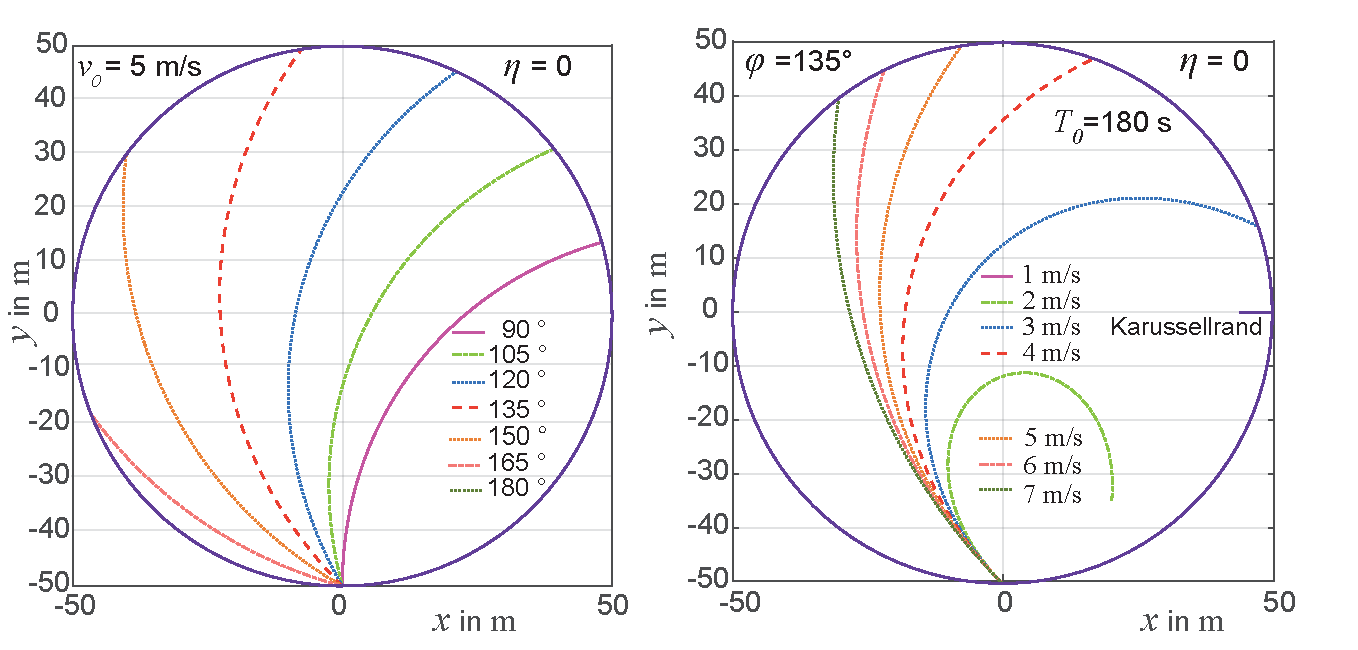
\includegraphics[width=\textwidth]{Lsg_Scheibe02.pdf}%
\caption[Trajektorien eines bewegten K�rpers auf einem  Karussell.]{Trajektorien eines bewegten K�rpers auf einem sich gleichm��ig drehenden Karussell f�r verschiedene Richtungen $\alpha$ der Anfangsgeschwindigkeit $v_0 = 5\, \mathrm{m s^{-1}}$ (Abb. links) und f�r verschiedene Anfangsgeschwindigkeiten $v_0 $ bei festgehaltener Richtung}
\label{abb:bew_Lsg_Scheibe02}
\end{figure}

\begin{figure}[H]\centering
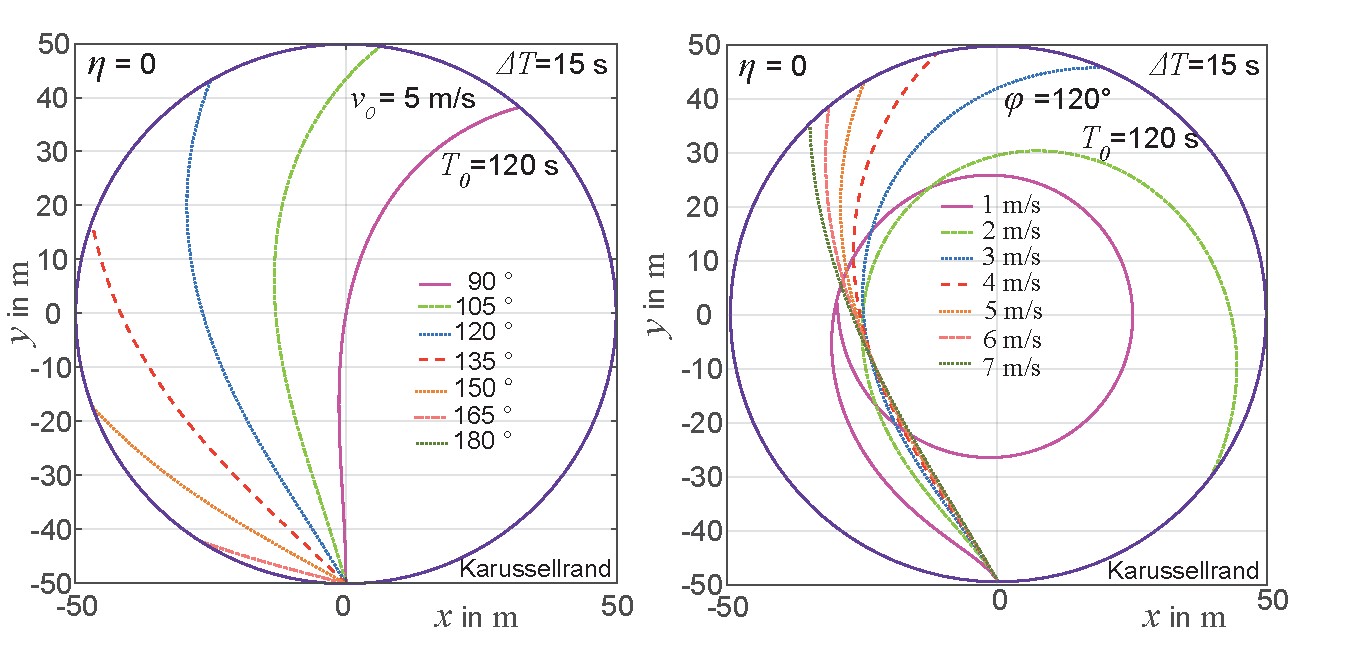
\includegraphics[width=\textwidth]{Lsg_Scheibe03.pdf}%
\caption[Trajektorien auf einem beschleunigenden Karussell]{Trajektorien eines bewegten K�rpers auf einem sich in der Rotation beschleunigenden Karussell. f�r verschiedene Richtungen $\alpha$ der Anfangsgeschwindigkeit $v_0 = 5\, \mathrm{m s^{-1}}$ (Abb. links) und f�r verschiedene Anfangsgeschwindigkeiten $v_0 $ bei festgehaltener Richtung. Das Karussell erreicht nach einer initialen Beschleunigungszeit von 15 s die dann konstante Rotationsperiode von 120 s}
\label{abb:bew_Lsg_Scheibe03}
\end{figure}

\end{subprobs}
\end{sol} 
%\href{PhysikUncut_Part1.pdf#prb:bew_Coriolis_IV}{\textcolor{blue} {$\rightarrow$ zur \probref{bew_Coriolis_IV}.}}\\
\textcolor{blue} {$\rightarrow$ zur} \probref{bew_Coriolis_IV}.\\
\noindent\rule[1ex]{\textwidth}{0.5pt}  \newpage 



%%%-----------------------------------------------------------------------------------------------------------
%%%-----------------------------------------------------------------------------------------------------------
\newpage

\subsection{�bungen zu Streuproblemen}

\medskip

%-----------------------------------------------------------------------------------------------------------
\hypertarget{lsg:bew_Rutherford}{}
\begin{sol}{prob:bew_Rutherford}\label{lsg:bew_Rutherford} %�bung22
\textbf{Rutherford-Streuung} \\ \\
Die L�sung ist im Detail in den \mscren\mlbewref{RutherfordAlpha.m} und \mlbewref{RutherfordAg.m} beschrieben.
Beispiell�sungen sind f�r $\alpha$- und Silber-Teilchen verschiedener Energien in der Laborsystem-Darstellung in \figref{bew_Rutherford02} gezeigt.

\begin{figure}[H]\centering
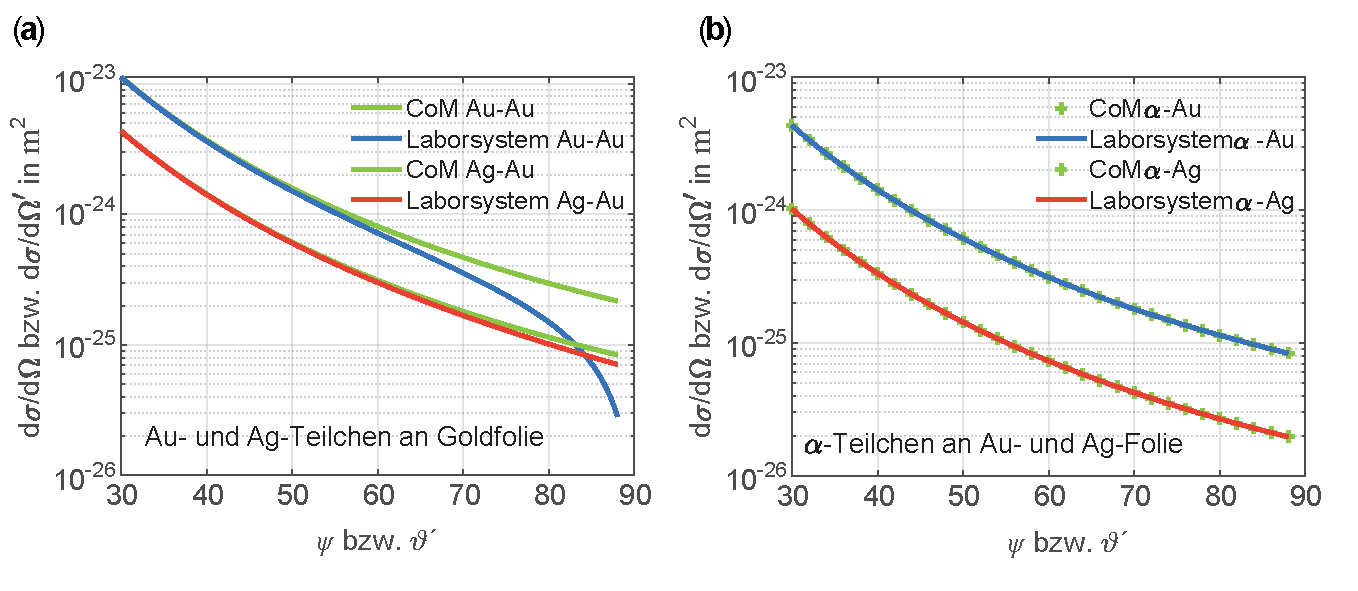
\includegraphics[width=\textwidth]{Rutherford02.pdf}
\caption[Streuung von $\alpha$- und Silber-Teilchen im Coulomb-Feld]{Streuung von \fa $\alpha$- und \fb Silber-Teilchen im Coulomb-Feld von Gold-Atomkernen f�r verschiedene Einfallsenergien (numerische Simulation). Als Ma�einheit f�r die Raumkoordinaten wurde der Bohr-Radius mit $a_\text{B} = \SI{5.29177e-11}{\metre}$ gew�hlt. Man erkennt in dieser Laborsystem-Darstellung sehr sch�n den R�cksto�effekt bei den schwereren Silberteilchen} 
\label{abb:bew_Rutherford02}
\end{figure}

\end{sol} 
%\href{PhysikUncut_Part1.pdf#prb:bew_Rutherford}{\textcolor{blue} {$\rightarrow$ zur \probref{bew_Rutherford}.}}\\
\textcolor{blue} {$\rightarrow$ zur} \probref{bew_Rutherford}.\\
\noindent\rule[1ex]{\textwidth}{0.5pt}  \newpage


%-----------------------------------------------------------------------------------------------------------
\hypertarget{lsg:bew_Asteroid}{}
\begin{sol}{prob:bew_Asteroid}\label{lsg:bew_Asteroid} %�bung23 
\textbf{Asteroiden-Auftreffwahrscheinlichkeit auf einen Planeten} \\ \\
Wir beschreiben die Bewegung der Asteroiden im KOS, dessen Nullpunkt im Zentrum des Planeten liegt (\figref{bew_astcoll01}) und betrachten nur die Gravitationswirkung des Planeten, d.\,h. wir vernachl�ssigen die Gravitation der Sonne und der anderen Planeten.\\

\begin{figure}[H]\centering
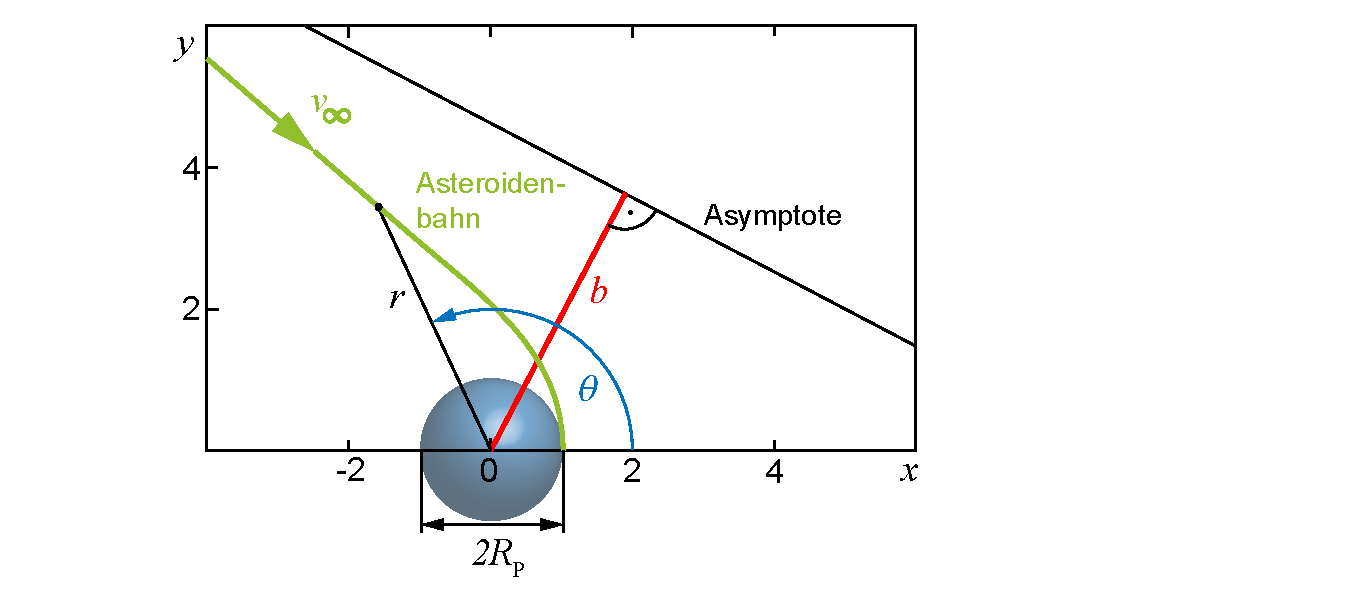
\includegraphics[width=\textwidth]{AsteroidColl01.pdf}
\caption{Streuung eines Asteroiden im Schwerefeld eines Planeten} 
\label{abb:bew_astcoll01}
\end{figure}

Der spezifische (auf die Masse bezogene) Drehimpuls ($L \equiv L/m$) des Asteroiden gegen�ber dem Planetenzentrum ist 
        \begin{align}
            L = v_\infty \,b \,, \label{eq:bew_astcoll01}
        \end{align}
worin $v_\infty$ die Geschwindigkeit des Asteroiden weit ab vom Planeten ist. Die spezifische (wiederum auf die Masse bezogene) Energie ($E \equiv E(r)/m$) des Asteroiden Energie im $\infty$ ist $E_\infty=\frac{m}{2}\,{v_\infty}^2$, so dass 
        \begin{align*}
            E(r) = -\frac{G\,m_\text{P}}{r} + \frac{1}{2}\,\lek v\lk r\rk\rek^2 = E_\infty = \frac{1}{2}\,{v_\infty}^2\,,
        \end{align*}
woraus die Energie im Abstand $r$
        \begin{align}
            \lek v\lk r\rk\rek^2 = {v_\infty}^2 + \frac{2G\,m_\text{P}}{r} \label{eq:bew_astcoll02}
        \end{align}
folgt. Wir haben dabei die auf die Masse $m$ des Asteroiden bezogenen Gr��en verwendet. \\
In diesem Streuproblem bewegt sich der Asteroid nach \eqref{eq:bew_Bahn_explizit} auf einer Hyperbelbahn:
        \begin{align}
            r = \frac{L^2}{G\,m_\text{P}}\, \frac{1}{1+e\,\cos\theta}\,, \label{eq:bew_astcoll03}
        \end{align}
deren Exzentrizit�t $\epsilon$ durch \eqref{eq:bew_Bahn_Exzentrizitaet} 
        \begin{align}
            \epsilon = \sqrt{1+\frac{2\,E\,L^2}{\lk G\,m_\text{P}\rk^2}} = \sqrt{1+\frac{{v_\infty}^4 b^2} {\lk G\,m_\text{P}\rk^2}} \label{eq:bew_astcoll04}
        \end{align}
gegeben ist. Der minimale Abstand wird bei $r_\text{min}\lk\theta = 0 \rk$ erreicht, also bei\\
$L^2/\lk G\,M\rk = r_\text{min}\lk 1+\epsilon\rk$,\\
so dass wir f�r \eqref{eq:bew_astcoll03} schreiben k�nnen:
        \begin{align}
            r\lk \theta\rk = \frac{r_\text{min}\lk 1+\epsilon\rk}{1+\epsilon\,\cos\theta}\,. \label{eq:bew_astcoll05}
        \end{align}
Ferner gilt f�r die Hyperbel die Beziehung \eqref{eq:bew_hyp_asymptote}) woraus man
        \begin{align*}
            b = r_\text{min}\,\sqrt{\frac{\epsilon+1}{\epsilon-1}}1\,
        \end{align*}
herleiten kann. Abh�ngig von den Parametern $m_\text{P}$, $v_\infty$ und $b$ und dem Radius $R_\text{P}$ kann es unter Umst�nden zu einer Kollision kommen, und zwar dann wenn $r_\text{min}\leq R_\text{P}$ bzw. 
	\[\frac{r_\text{min}}{R_\text{P}} = \frac{b}{R_\text{P} \sqrt{\frac{\epsilon-1}{\epsilon+1}} < 1} \,.
	\]
	Durch die Gravitation ist der Streuquerschnitt der Kollision um einen Faktor $\gamma$ gr��er als rein geometrisch gegeben, 
        \begin{align}
            \gamma = \frac{\pi\,b^2}{\pi\,{R_\text{P}}^2} = \lk \frac{b}{R_\text{P}} \rk^2 \,. \label{eq:bew_astcoll07}
        \end{align}
Beim Erreichen des minimalen Abstands $r_\text{min} = R_\text{P}$ zum Planeten hat der Asteroid folgende Energie
        \begin{align*}
            {v_\infty}^2 +\frac{2G\,m_\text{P}}{R_\text{P}} = v\lk r_\text{min}\rk^2 = {v_\text{r,min}}^2\,.
         \end{align*}
Ferner gilt Drehimpulserhaltung: $ v_\infty\,b = v_\text{r,min}\,R_\text{P} \,.$
Wir ersetzen $v_\text{r,min}$ und erhalten: 
        \begin{align*}
            {v_\infty}^2 + \frac{2G\,m_\text{P}}{R_\text{P}} = \lk \frac{b}{R}\rk^2\,{v_\infty}^2\,.
        \end{align*}
Das kann man schreiben als 
        \begin{align}
            \gamma = 1 + \frac{\lk \sqrt{\frac{2G\,m_\text{P}}{R_\text{P}}}\rk^2}{{v_\infty}^2} = 1+\lk \frac{v_\text{F}}{v_\infty}\rk^2 \,, \label{eq:bew_astcoll08}
        \end{align}
worin $v_\text{F}$ die sogenannte \gls{vescape} vom jeweiligen Planeten ist. Gleichung \eqref{eq:bew_astcoll08} besagt also, dass der Kollisionsquerschnitt umso gr��er ist, je gr��er die Fluchtgeschwindigkeit und je kleiner die \glqq Einfallsgeschwindigkeit \grqq{} $v_\infty$ des Asteroiden ist (Tabelle \ref{tab:bew_astcoll01}).

\begin{table}[h!]
\centering
\begin{tabular}{|L{1.2cm}|C{2cm}|C{2cm}|C{2cm}|}
\hline
%\rule{0pt}{3pt}& & &   \\
  & $R_\text{P}$  & $v_\text{esc}$ & $\gamma$ \\
\rule{0pt}{3pt}& km & km/s &  \\
\hline
%\rule{0pt}{3pt}& & &  \\
\rule{0pt}{6pt}Erde   & $\SI{6378}{}$ & $\SI{11.2}{}$ & $\SI{2.25}{}$  \\
\rule{0pt}{6pt}Mars & $\SI{3397}{}$  & $\SI{5.0}{}$ & $\SI{1.25}{}$ \\
\rule{0pt}{6pt}Jupiter  & $\SI{71492}{}$ & $\SI{59.5}{}$ & $\SI{36.45}{}$ \\
%\rule{0pt}{3pt}& & &  \\
\hline
\end{tabular}
\smallskip
\caption{Berechnete Werte f�r Asteroideneinfall auf verschiedene Planeten} \label{tab:bew_astcoll01}
\end{table}
\figref{bew_astcoll02} zeigt Trajektorien von parallel einfallenden Asteroiden aber unterschiedlichen Sto�parametern f�r die Planeten Jupiter und Erde in Einheiten des Radius des jeweiligen Planeten.
Die Einfallsgeschwindigkeit wurde in beiden F�llen zu $\SI{14.0}{\km\per\s}$ angenommen.
Man erkennt, dass der Jupiter wie erwartet einen deutlich gr��eren Kollisionsquerschnitt hat.
Zur Vertiefung empfehlen wir \mlbewref{AsteroidKollision.m}, \mlbewref{AsteroidStreuung.m} und \cite{VanAllen2006}.
\begin{figure}[H]\centering
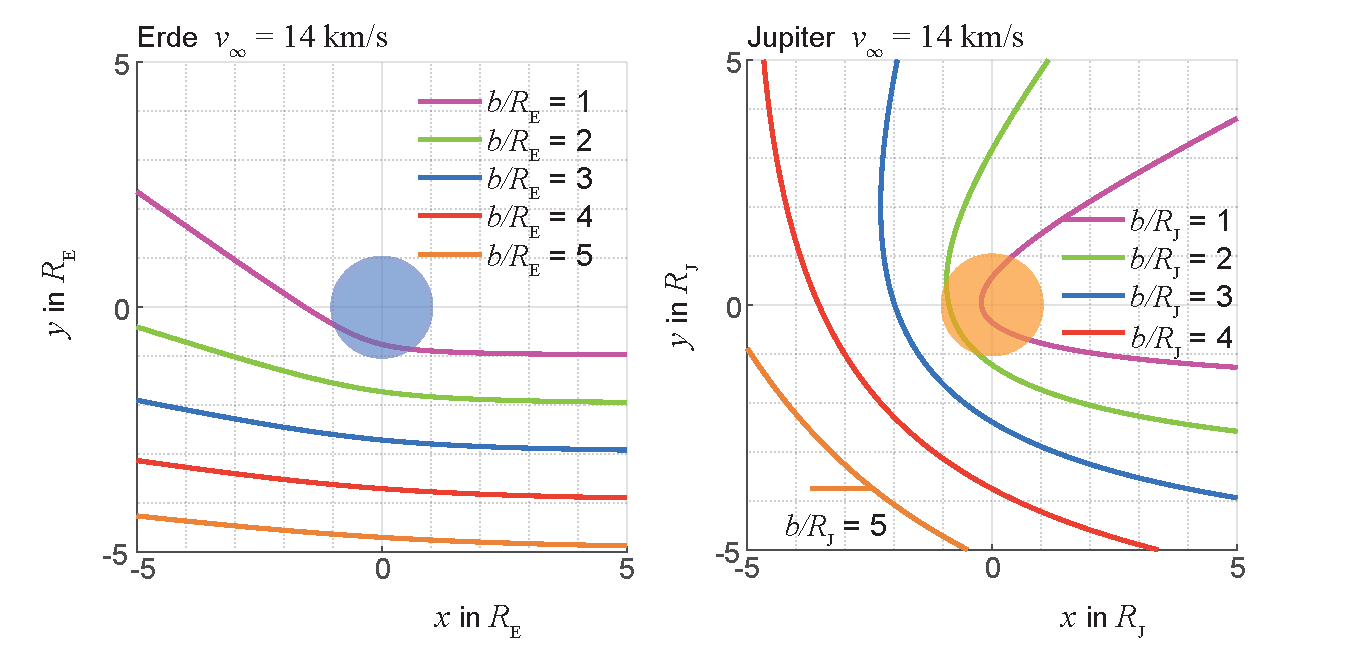
\includegraphics[width=\textwidth]{AsteroidColl02.pdf}
\caption[Trajektorien von einfallenden Asteroiden f�r Jupiter und Erde]{Trajektorien von einfallenden Asteroiden f�r Jupiter und Erde in Einheiten des Radius des jeweiligen Planeten} 
\label{abb:bew_astcoll02}
\end{figure}

\smallskip
\end{sol} 
%\href{PhysikUncut_Part1.pdf#prb:bew_Asteroid}{\textcolor{blue} {$\rightarrow$ zur \probref{bew_Asteroid}.}}\\
\textcolor{blue} {$\rightarrow$ zur} \probref{bew_Asteroid}.\\
\noindent\rule[1ex]{\textwidth}{0.5pt}  \newpage


%%%-----------------------------------------------------------------------------------------------------------
%%%-----------------------------------------------------------------------------------------------------------
\newpage

\subsection{�bungen zu Oszillatoren und Pendel}

\medskip
%-----------------------------------------------------------------------------------------------------------
\hypertarget{lsg:bew_PendelGl}{}
\begin{sol}{prob:bew_PendelGl}\label{lsg:bew_PendelGl} %�bung24
\textbf{Pendelgleichungen} \\ \\
Wir starten von \eqref{eq:bew_Schwingung01b} und betrachten ein Pendel mit der Fadenl�nge $l$, an dem eine Masse $m$ aufgeh�ngt ist.
Die generalisierte Koordinate ist der Winkel $\varphi$. 
Aus $x = l \sin\varphi$ und $z = -l \cos\varphi$ folgt 
\begin{align*}
		h\lk \varphi \rk &= \lk \frac{\d x}{\d \varphi} \rk^2 + \lk \frac{\d z}{\d \varphi} \rk^2 = l^2 \,, \\
		U \lk \varphi \rk &= -m g l \cos\varphi \,, \\
		&= -m g l\,\lk 1-\frac{1}{2}\cos^2\varphi\, \big|_{\varphi=0}\,\varphi^2+\frac{1}{24} \cos^4\varphi \,\big|_{\varphi=0}\, \varphi^4 + \sum_k \frac{\lk -1 \rk^k}{\lk 2k \rk !}\varphi^{2k}\rk.
\end{align*}
Hierbei haben wir im Potential nur die von Null verschiedenen Terme mitgenommen, den ersten Term $-m\,g\,l$ k�nnen wir ohne weiteres \anf{wegeichen}.
Da bei dem Pendel $h\lk \varphi \rk = \text{const} = l^2$ ist, gilt f�r die Bewegungsgleichung
\begin{align}
		m\,\frac{\D}{\D t}\lk l^2\,\dot{\varphi}\rk + \frac{\d U\lk \varphi \rk}{\d \varphi} &= 0 \,, \\
		m\,l^2\,\ddot{\varphi} + m\,g\,l\,\frac{\d}{\d \varphi} \lk \frac{1}{2} \varphi^2-\frac{1}{24} \varphi^4 + \sum_k \frac{\lk -1 \rk^k}{\lk 2k \rk !}\varphi^{2k}\rk &= 0 \,, \\
		\ddot{\varphi} + \frac{g}{l} \lk \varphi - \frac{1}{6} \varphi^3 + \sum_k \frac{\lk -1 \rk^k}{\lk 2k-1 \rk !}\varphi^{2k-1}\rk &= 0 \,.
\end{align}
Wir haben also die Bewegungsgleichung des Pendels als Reihe aufschreiben k�nnen.
Dies legt nahe, dass wir auch die Schwingungsperiode $T_\text{P} = 2\pi\sqrt{\frac{l}{g}}$ als Reihe entwickeln k�nnen.


\end{sol} 
%\href{PhysikUncut_Part1.pdf#prb:bew_PendelGl}{\textcolor{blue} {$\rightarrow$ zur \probref{bew_PendelGl}.}}\\
\textcolor{blue} {$\rightarrow$ zur} \probref{bew_PendelGl}.\\
\noindent\rule[1ex]{\textwidth}{0.5pt}  \newpage


%-----------------------------------------------------------------------------------------------------------
\hypertarget{lsg:bew_HO_quadrat}{}
\begin{sol}{prob:bew_HO_quadrat}\label{lsg:bew_HO_quadrat} %�bung25
\textbf{Harmonischer Oszillator mit quadratischem Reibungsterm.} \\

Die Bewegungsgleichungen lauten f�r den (eindimensionalen) harmonischer Oszillator mit quadratischem Reibungsterm (Newton-Reibung):
\begin{align}
			m\,\ddot{q} &= - m\,{\omega_0}^2\,q  - m \, \eta_\text{N}\,\mathrm{sign}(\dot{q})\,\dot{q}^2 \,. \label{eq:bew_HO_quadfriction01}
\end{align}
Es ist zu beachten, dass der Reibungsterm das Vorzeichen jedes mal wechselt, wenn $\dot{q}=0$, \dh zweimal pro voller Schwingung.
Dies wird durch die Signum-Funktion ber�cksichtigt und muss bei der \matlab{} Programmierung entsprechend beachtet werden.
Diese ist in \mlbewref{HarmonOszQuadReibung.m} ausgef�hrt.
Zur Erinnerung die Bewegungsgleichung des harmonischen Oszillator mit linearem Reibungsterm (Stokes-Reibung) \eqref{eq:bew_pendulum02}:
\begin{align}
			m\,\ddot{q} &= - m\,{\omega_0}^2\,x  - m \, \eta_\text{S}\,\dot{q} \,. \label{eq:bew_HO_quadfriction02}
\end{align}
Das Ergebnis der Integration der beiden Bewegungsgleichungen ist im Vergleich zum unged�mpften Fall in \figref{bew_HO_quadrat01} zu sehen, \figref{bew_HO_quadrat02} zeigt die Energieabnahme des jeweiligen Oszillators �ber die Zeit.
\begin{figure}[H]\centering
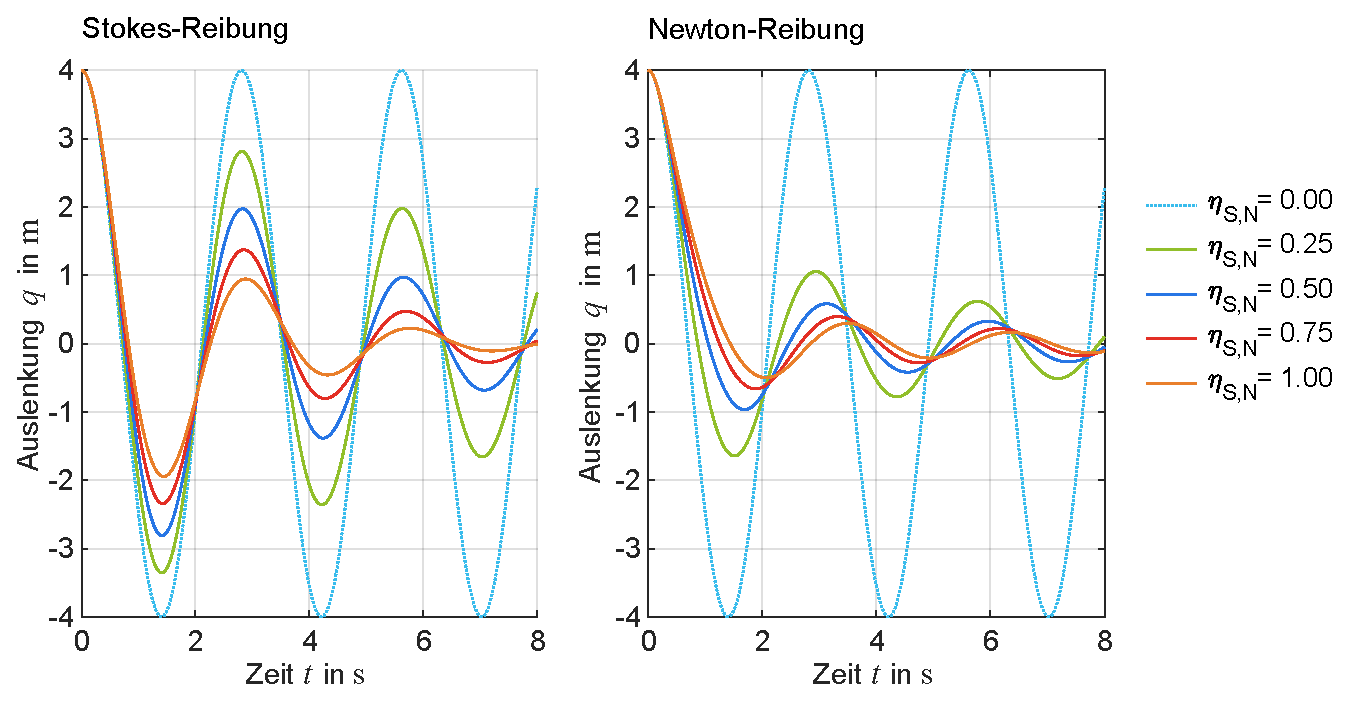
\includegraphics[width=\textwidth]{HO_Quadrat01.pdf}%
\caption[L�sung der Bewegungsgleichung f�r den harmonischer Oszillator]{Vergleich der L�sungen der Bewegungsgleichung f�r den harmonischer Oszillator mit quadratischen Reibungsterm (Newton-Reibung) (rechts) und linearem Reibungsterm (Stokes-Reibung) f�r verschiedene Parameter (links)}
\label{abb:bew_HO_quadrat01}
\end{figure}
\begin{figure}[H]\centering
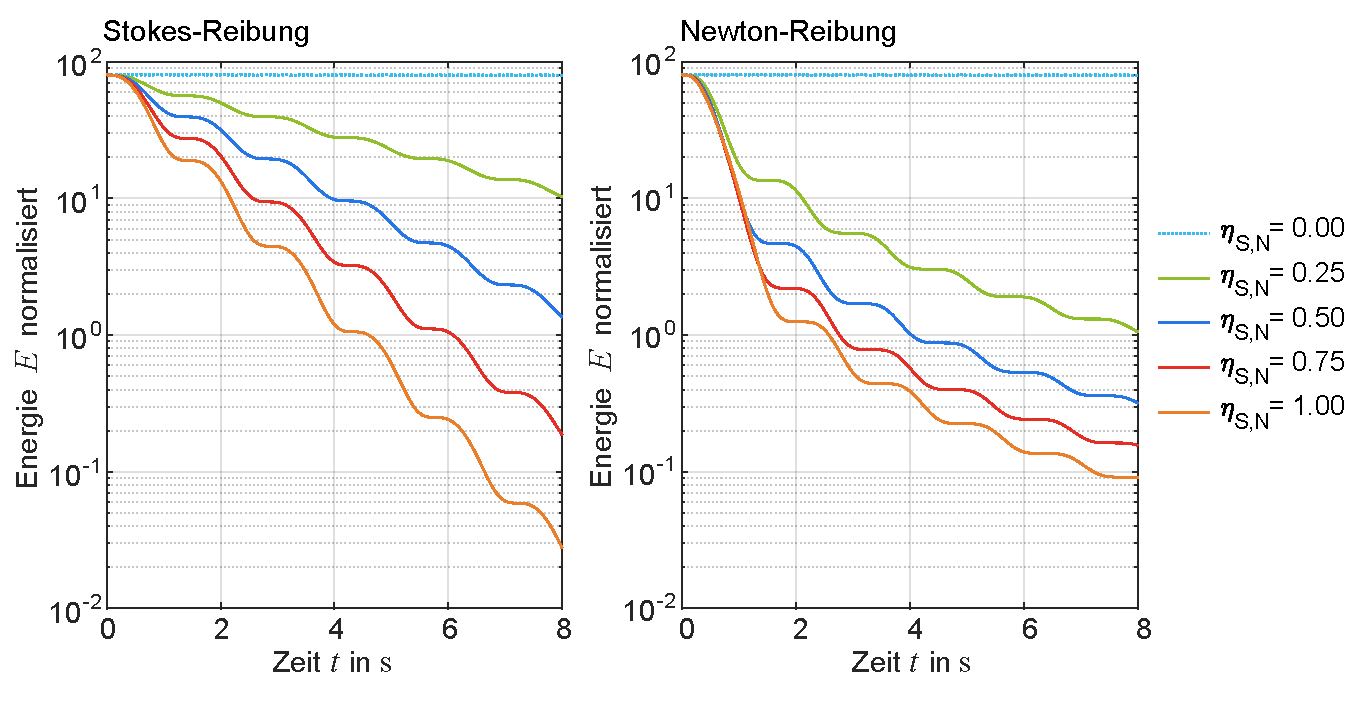
\includegraphics[width=\textwidth]{HO_Quadrat02.pdf}%
\caption[Energiedissipation des harmonischen Oszillators]{Energiedissipation des harmonischen Oszillators mit quadratischen Reibungsterm (Newton-Reibung) f�r verschiedene Parameter (rechts) und im Vergleich zur Energiedissipation beim Oszillator mit Stokes-Reibung (links)}
\label{abb:bew_HO_quadrat02}
\end{figure}

Man erkennt, dass beim harmonischen Oszillator mit quadratischem Reibungsterm die Frequenz $\omega$ wie auch die Energieabnahme stark von den Anfangsbedingungen abh�ngen. Die Schwingungsperiode $T_P$ ist dar�ber hinaus stark von der Eigenfrequenz $T_{P0}=2\pi/\omega_0$ verschieden und auch noch von der Zeit abh�ngig. Die Energiedissipation beim harmonischen Oszillator passiert zu Beginn viel schneller. Ist aber ein niedriges Niveau erreicht, dann dissipiert die Energie des Systems deutlich langsamer als im linearen Reibungsfall. 
F�r interessierte Leser sei die relativ komplizierte analytische L�sung in \cite{Smith2012} zur Lekt�re empfohlen.
\end{sol} 
%\href{PhysikUncut_Part1.pdf#prb:bew_HO_quadrat}{\textcolor{blue} {$\rightarrow$ zur \probref{bew_HO_quadrat}.}}\\
\textcolor{blue} {$\rightarrow$ zur} \probref{bew_HO_quadrat}.\\
\noindent\rule[1ex]{\textwidth}{0.5pt}  \newpage


%-----------------------------------------------------------------------------------------------------------
\hypertarget{lsg:bew_ExamplesHO}{}
\begin{sol}{prob:bew_ExamplesHO}\label{lsg:bew_ExamplesHO} %�bung26
\textbf{Beispiele f�r harmonische Schwingungen (\vgl auch \cite{Hasbun2018}.).} 

\begin{figure}[H]\centering
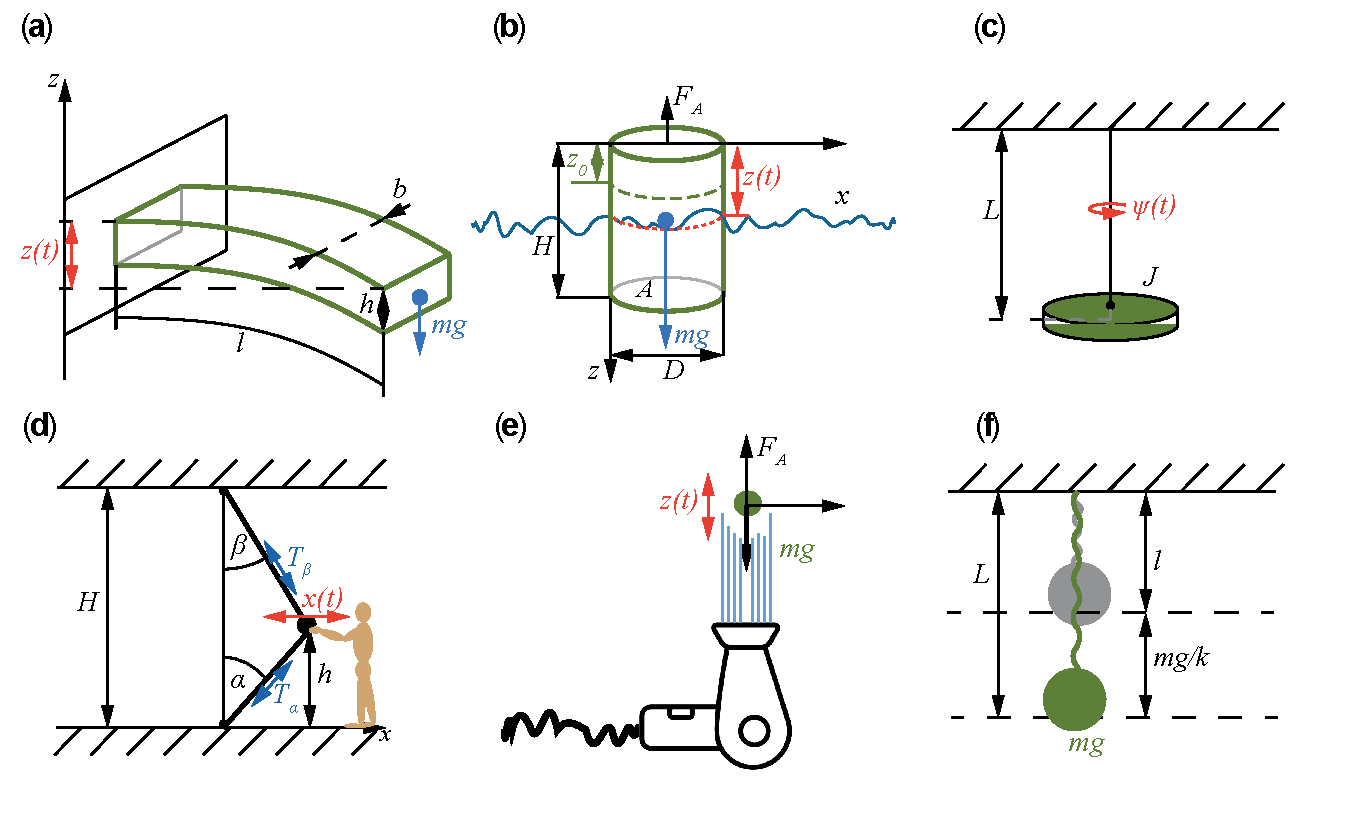
\includegraphics[width=\textwidth]{BeispieleHO.pdf}
\caption[Beispiele f�r harmonische Schwingungen]{Beispiele f�r harmonische Schwingungen} 
\label{abb:bew_HOex02}
\end{figure}

\begin{subprobs}
\subprob{Sprungbrett (\figref{bew_HOex02}\,a)}
Wir werden im Kapitel Kontinuumsmechanik (\ref{chap:kontmech}) sehen, dass die Auslenkung $z$ eines Balkens bei einer wirkenden Kraft $F$ gegeben ist durch:
	\begin{align*}
			 z = -\frac{L^3\, 12}{3Y\,b\,h^3}\,F = -4\,\frac{l^3}{b\,h^3}\,\frac{F}{Y}\,.
	\end{align*}
Hierin sind $Y$ der Young-Elastizit�tsmodul\footnote{Thomas Young\indexp{Young, Thomas} (1773--1829) war ein englischer Augenarzt und Physiker. Young forschte zur Wellennatur und insbesondere zur Interferenz des Lichts. Ber�hmt ist sein Doppelspaltexperiment, welches sp�ter f�r die Entwicklung der Quantenmechanik eine wichtige Rolle spielte.}
und $l,b,h$ die L�nge, Breite \bzw H�he des Balkens.
Wir haben also $z \propto F$. \\
Wenn man jetzt die Kraft am Ende des Balkens durch eine fest angebrachte Masse  $m=\SI{100}{\kg}$ hervor gebracht denkt, dann ist die Gleichgewichtslage durch 
\[z_0 = -\frac{4L^3}{b\,h^3}\frac{m\,g}{Y}\]
gegeben. 
Der Balken kann dann als schwingendes System um die neue Gleichgewichtslage betrachtet werden.
Die Bewegungsgleichung f�r die am Balkenende befestigte Masse $m$ lautet: 
		\begin{align}
				m\,\ddot{z} = -\frac{Y\,b\,h^3}{4L^3}\lk z-z_0\rk \,. \label{eq:bew_HOexL01}
		\end{align}

\newpage
Die Schwingungsfrequenz	ist gegeben durch
		\begin{align*}
				\omega = \sqrt{\frac{Y\,b\,h^3}{4m\,l^3}}\,.
		\end{align*}
Ein typisches Sprungbrett mit $l = \SI{5}{\metre}$, $h = \SI{10}{\cm}$ und $b = \SI{1}{\metre}$ aus Holz mit dem Elastizit�tsmodul $Y = \SI{1e09}{\newton\per\square\metre}$ hat also eine Schwingungsperiode von etwa $T_\text{P}=2\pi/\omega=\SI{1.4}{\second}$. \\ %Masse war nicht gegeben

\subprob{Tonne im Wasser (\figref{bew_HOex02}\,b)} \\
Im Gleichgewicht entspricht der Auftrieb dem verdr�ngtem Wassergewicht, also
		\begin{align*}
				F_\text{A0} = \varrho_\text{W} A \,\lk H-z_0 \rk g = m \,g \,,
		\end{align*}
woraus
		\begin{align*}
				z_0 = H-\frac{m}{\varrho_\text{W}A} 
		\end{align*}
folgt. 
Kommt es zu einer kleinen Verschiebung $\Delta z = z-z_0$ aus der Gleichgewichtslage, so ver�ndert sich auch die Auftriebskraft:
		\begin{align*}
				\Delta F = F_\text{A} -F_\text{A0} = \varrho_\text{W}\,A\,g\,\lek\lk H-z\rk-\lk H-z_0\rk\rek\,.
		\end{align*}
Aus dem zweiten Newtonschen Axiom folgt dann f�r die Tonnenh�he oberhalb des Wassers $z$:
		\begin{align*}
				m \,\ddot{z} &= F_\text{A}(z)-m\,g = F_\text{A}(z) -F_\text{A0}(z_0) \,,\\
				m \,\ddot{z} &= \varrho_\text{W}\,g\,A\lk z-z_0\rk \,.
		\end{align*}
Wir setzen $z-z_0 = +\,\xi$ bei $z_0<0$ und erhalten
		\begin{align*}
				\ddot{\xi} &= -\frac{\varrho_\text{W}\,g\,A}{m} \xi \,, \\
				\omega &= \sqrt{\frac{\varrho_\text{W}\,g\,A}{m}} \,.
		\end{align*}
Die Tonne schwingt also umso heftiger je geringer Ihre Masse ist und je gr��er ihr Durchmesser.

\subprob{Torsionspendel (\figref{bew_HOex02}\,c)}
Man kann die Bewegungsgleichung der linearen Feder in Analogie auf das Torsionspendel �bertragen.
D.h. die Parameter Masse $m$, Federkonstante $k$ und Auslenkung $x$ einer linearen Feder entsprechen den Parametern Tr�gheitsmoment $J$ (Einheit $\SI{}{\kg\square\meter}$), Direktionsmoment $D$ (Einheit  $ \SI{}{\newton\meter\per\radian}$) und Auslenkungswinkel $\varphi$ (Einheit $ \SI{}{\radian} $). 
Das Direktionsmoment ist -- wie auch die Federkonstante -- eine Materialeigenschaft des Drahtes. 
Damit lautet die Bewegungsgleichung $J\,\ddot{\varphi} + D\,\varphi = 0$, wobei $J$ auf die Achse bezogen ist, die durch die Aufh�ngung gegeben ist. 
F�r einen Draht mit Radius $r_\text{D}$ und L�nge $L$ (ohne Scheibe) gilt:
		\begin{align*}
				D = \frac{\pi r_\text{D}^4}{2}\frac{G_\text{S}}{L} \,.
		\end{align*}
Die Gr��e $G_\text{S}$ ist dabei das Schubmodul, welches wiederum mit der Poissonzahl\index{Poissonzahl}\footnote{Sim�on Denis Poisson (1781--1840 in Paris) war ein franz�sischer Physiker und Mathematiker. Er war Sch�ler von Laplace und besch�ftigte sich vor allem mit der Theorie der Wellen in der Akustik, der Elastizit�ts- und W�rmelehre, sowie der Potentialtheorie der Elektrostatik. Als Mathematiker arbeitete Poisson vor allem auf den Gebieten der Differentialgeometrie, der Infinitesimal- und Wahrscheinlichkeitsrechnung. Mehrere mathematische Begriffe sind mit seinem Namen verbunden. Er war sehr produktiv und ver�ffentlichte insgesamt �ber 300 Arbeiten.}\indexp{Poisson, Sim�on Denis} $\mu$ (ein Wert zwischen 0 und 0.5) �ber $G_\text{S} = \frac{1}{2(1+\mu)}\,Y$ direkt proportional zum Elastizit�tsmodul $Y$ ist. 
Die Frequenz ergibt sich dann zu 
		\begin{align*}
				\omega = \sqrt{\frac{D}{J}} \,.
		\end{align*}
F�r eine zentrisch aufgeh�ngte Scheibe gilt $J = \frac{1}{2}m_\text{s}R_\text{s}^2$ und damit erh�lt man
		\begin{align*}
				\omega = \frac{r_\text{D}^2}{R_\text{s}}\sqrt{\frac{G_\text{S}}{L}\frac{\pi}{m_\text{s}}}
		\end{align*}
f�r die Kreisfrequenz. \\
Torsionspendel haben in der Zeitmessung eine gro�e Rolle gespielt.
Das liegt vor allem daran, dass der Zusammenhang zwischen dem r�cktreibenden Moment $D_\varphi$ und der Auslenkung $\varphi$ im Gegensatz zum mathematischen Pendel oder der linearen Feder nicht nur f�r kleine Winkel linear ist.

\subprob{Zugseil im Fitnessstudio (\figref{bew_HOex02}\,d)}
Aus der \figref{bew_HOex02}d k�nnen wir die Spannung im Seil in guter N�herung f�r kleine Winkel $\alpha$ und $\beta$ als konstant ansehen, also $T = T_\alpha = T_\beta$.
Aus der Geometrie in der Abb. folgt somit f�r die $x$-Komponente der Seilspannung als r�cktreibende Kraft:
		\begin{align*}
					m\,\ddot{x} &= -T_\alpha\sin\!\alpha(t)-T_\beta\sin\!\beta(t) = -T\, \lk \frac{x}{\sqrt{x^2+h^2}}+\frac{x}{\sqrt{x^2+\lk H-h\rk ^2}}\rk \,.
		\end{align*}
F�r $x \ll h$ gilt die N�herung	
	\begin{align*}
			m\,\ddot{x} &\approx - T \, \lk\frac{x}{h}+\frac{x}{H-h}-\mathcal{O}(x^3)\rk\\
			\rightarrow m\,\ddot{x} &= - \frac{T\,H}{h\lk H-h\rk}\,x  \\
			\rightarrow \omega &= \sqrt{\frac{T}{m}\frac{H}{h\lk H-h\rk}}\,.
	\end{align*}
F�r $h = \frac{H}{2}$ folgt:
	\begin{align*}
			&m\,\ddot{x} + 4\,\frac{T}{H}\,x = 0 \,, \\
			\rightarrow \omega &= \sqrt{\frac{4T}{m\,H}} 
			\qquad \text{with} \quad m = \varrho^\text{(L)}H \\
			&= \sqrt{\frac{4T}{\varrho^\text{(L)}H^2}} 
			= \frac{2}{H}\sqrt{\frac{T}{\varrho^\text{L}}}\,.
	\end{align*}
Man �berlege sich, was dieser Ausdruck physikalisch bedeutet.
Hinweis: $f = {\omega}/{2\pi}= {c_\text{ph}}/{\lambda}$. \\

\subprob{Tischtennisball im F�n (\figref{bew_HOex02}\,e)}
Wir werden in der Mechanik der Kontinua (\autoref{chap:kontmech}) die Bernoulli%
\footnote{Daniel Bernoulli\indexp{Bernoulli, Daniel} (1700--1782) war ein Schweizer Mathematiker und Physiker aus der Gelehrtenfamilie der Bernoullis. Er arbeitete auf vielen Gebieten u.a. mit Leonhard Euler. Die nach ihm benannte Bernoulli-Gleichung ist von zentraler Bedeutung in der Hydro- und Aerodynamik.}-Gleichung kennenlernen,
die den Fluss laminarer, nichtkompressibler Fl�ssigkeiten und Gase beschreibt. 
Die Str�mungsgeschwindigkeit des Luftstroms sei $v(z)$, die Masse des Tischtennisballs $m$ und die Bewegungskoordinate $z$. 
Beim Austritt aus dem F�n gelte $v(z=0) = v_\text{A}$. 
Dann gilt f�r die Geschwindigkeit $v_\text{A}$ der Luftmolek�le nach der Bernoulli-Gleichung%
\footnote{Man kann die Bernoulli-Gleichung auch als Energieerhaltung von spezifischer kinetischer und potentieller Energie deuten.}:
		\begin{align*}
				\frac{1}{2} \varrho\,{v_\text{A}}^2 &= \frac{1}{2} \varrho\,v(z)^2+\varrho\,g\,z \,, \\
				\rightarrow v(z) &= v_\text{A} \sqrt{1-\frac{2g\,z}{{v_\text{A}}^2}} \approx v_\text{A} \lk 1-\frac{g\,z}{{v_\text{A}}^2}\rk \,.
		\end{align*}
Auf den Tischtennisball wirkt die Gewichtskraft und die (Stokes-)Reibungskraft, also gilt:
		\begin{align*}
				F=m\,\ddot{z} &= -m\,g+\eta\,v(z) \,, \\
				\rightarrow m\,\ddot{z} &= -m\,g + \eta\,v_\text{A} \lk 1 -\frac{g\,z}{{v_\text{A}}^2} \rk \,.
		\end{align*}
Im Gleichgewicht $z=z_0$ muss $F=-m\,g+\eta\,v(z_0) = 0$ sein, woraus folgt:
		\begin{align*}
				v(z_0) &= \frac{m\,g}{\eta} = v_\text{A}\lk 1-\frac{g\,z_0}{{v_\text{A}}^2}\rk ~~ \text{und daher} \\
				z_0 &= v_\text{A} \lk \frac{v_\text{A}}{g}-\frac{m}{\eta}\rk.
		\end{align*}
Somit lautet die Bewegungsgleichung und die entsprechende Frequenz
		\begin{align*}
				\ddot{z} + \frac{\eta\,g}{m\,v_\text{A}}\lk z-z_0\rk = 0 
				\quad \text{mit} \quad 
				\omega = \sqrt{\frac{\eta\,g}{m\,v_\text{A}}}\,.
		\end{align*}
Interessanterweise ist die Frequenz der Schwingung umso gr��er, je gr��er die D�mpfung $\eta$ (z.B. durch Reibung und/oder Viskosit�t) und umso kleiner die Austrittsgeschwindigkeit $v_\text{A}$ des Luftstromes ist.

\subprob{Feder mit Masse und ver�nderter Gleichgewichtslage (\figref{bew_HOex02}\,f)}
Aus der \figref{bew_HOex02}\,f k�nnen wir die Bewegungsgleichung bei ver�nderter Gleichgewichtslage direkt aufschreiben:
		\begin{align*}
				\ddot{z} +\omega^2 \lk z - z_\text{G}\rk = 0 \,.
		\end{align*}
Die Gleichung hat eine �hnliche Struktur und damit die gleiche L�sung wie \eqref{eq:bew_pendulum01}.
Allerdings sind die Konstanten der L�sung wegen der anderen Anfangsbedingungen neu zu bestimmen.
Wir schreiben die L�sung als
		\begin{align*}
				z &= z_\text{G} + A\sin\lk \omega t+\varphi\rk\,. \\
		\end{align*}
Mit $\dot{z} = A\, \omega\cos\lk \omega t+ \varphi\rk$ und \obda f�r $\varphi=0$ f�r $t=0$ erhalten wir:
		\begin{align*}
				\dot{z}_\text{max} &= A\,\omega = A\sqrt{\frac{k}{m}}v_\text{G} \,.
		\end{align*}
Das ist die Geschwindigkeit zum Zeitpunkt des Gleichgewichtsdurchgangs der Feder.\\
Wir wollen uns jetzt fragen, was ist die Amplitude nach oben, wenn die Feder v�llig entspannt ist, und was die Amplitude nach unten als Abstand von der Gleichgewichtslage ist, wenn die Feder maximal gedehnt ist:
		\begin{align*}
				E_\text{oben}  &= -m\,g\,l_\text{min} \,,~~~E_\text{unten} = \frac{k}{2} \lk l_\text{max}-l_\text{min}\rk^2-m\,g\,l_\text{max}\,.
		\end{align*}
Da die kinetische Energie in beiden F�llen Null ist, k�nnen wir $E_\text{oben} = E_\text{unten}$ setzen und nach $l_\text{max}(l_\text{min})$ aufl�sen und erhalten:
		\begin{align*}
				l_\text{max} = l_\text{min} +2\frac{m\,g}{k} = z_\text{G} +\frac{m\,g}{k} \,,
		\end{align*}
da in der Gleichgewichtslage $k\,z_\text{G}=m\,g$ ist. \\
Damit k�nnen wir schreiben
		\begin{align*}
				z &= \frac{m\,g}{k} \lk\, 1 + \sin\omega t \,\rk \,, ~~\dot{z} = \frac{m\,g}{k} \omega\cos\omega t \,, ~~\dot{z}_\text{max} = = \frac{g}{\omega}  = g\sqrt{\frac{m}{k}} \,.
		\end{align*}
Bisher haben wir die Masse der Feder vernachl�ssigt.
Das ist sicher im Allgemeinen erlaubt, aber bei starken Federn muss man ber�cksichtigen, dass die Feder auch bei der Bewegung eine kinetische Energie tr�gt.
Am einfachsten kann man den Fall modellieren, wenn man eine linear verteilte Masse der Feder annimmt.
Man kann dieses Problem nat�rlich numerisch l�sen.
%(siehe \cite{} und \scref{})  Noch einsetzen
Es hat sich aber gezeigt, dass man mit einer einfachen N�herungsformel f�r eine massebehaftete Feder �ber eine modifizierte Eigenfrequenz gute Ergebnisse erzielt (\cite{Hasbun2018}):
		\begin{align*}
				\omega \rightarrow \omega' = \sqrt{\frac{k}{m+{m_\text{F}}/{3}}} \,.
		\end{align*}
Man kann sich das leicht herleiten, indem man folgende lineare Geschwindigkeitsverteilung der Federmasse annimmt:
		\begin{align*}
				v_\text{F,max} &\approx \dot{z} = \dot{z}\lk z=l_\text{max}\rk \,,~~~v_\text{F,min} = 0 = v_\text{F}\lk z=0\rk \,.
		\end{align*}
Daraus folgt die kinetische Energie der Feder
		\begin{align*}
				T_\text{F} &= \frac{1}{2} {\varrho_\text{F}}^{(L)} \bigintsss\nolimits_0^{l_\text{max}} v\lk z'\rk^2 \D z' \,, \\
				 &=  \frac{1}{2} {\varrho_\text{F}}^{(L)} \bigintsss\nolimits_0^{l_\text{max}} \frac{\dot{z}^2\,{z'}^2}{{l_\text{max}}^2}\, \D z' = \frac{{\varrho_\text{F}}^{(L)} }{2}\frac{{l_\text{max}}^3}{3{l_\text{max}}^2}\,\dot{z}^2 = \frac{1}{2}\frac{m_\text{F}}{3}\,\dot{z}^2 \,.
		\end{align*}
Man k�nnte diesen Term zur Lagrange-Funktion $\mathcal{L}$ addieren, wodurch man eine Bewegungsgleichung mit einer effektiven Masse $m_\text{eff}=m + {m_\text{F}}/{3}$ erh�lt.


\end{subprobs}
\end{sol} 
%\href{PhysikUncut_Part1.pdf#prb:bew_ExamplesHO}{\textcolor{blue} {$\rightarrow$ zur \probref{bew_ExamplesHO}.}}\\
\textcolor{blue} {$\rightarrow$ zur} \probref{bew_ExamplesHO}.\\
\noindent\rule[1ex]{\textwidth}{0.5pt}  \newpage


%-----------------------------------------------------------------------------------------------------------
\hypertarget{lsg:bew_Molekuelpotentiale}{}
\begin{sol}{prob:bew_Molekuelpotentiale}\label{lsg:bew_Molekuelpotentiale} %�bung27
\textbf{Molek�lpotentiale.} \\
\begin{subprobs}
	\subprob{Lennard-Jones-Potential (Edelgas-Molek�le)}
	\begin{enumerate}[a)]
		\item Bindungsl�nge\\
			Aus dem Potential 
	\begin{align}
			U(q) = \lk \frac{A}{q^{12}} - \frac{B}{q^{6}} \rk = \lk \frac{4 \tilde{\epsilon}_\text{A} {q_0}^{12}}{q^{12}}
		-\frac{4 \tilde{\epsilon}_\text{B} {q_0}^{6}}{q^6} \rk  \label{eq:bew_Uebung22_00}
	\end{align}
			folgt 
			\[ U(\eta) = 4 (\tilde{\epsilon}_\text{A} \eta^2 - \tilde{\epsilon}_\text{B} \eta)\]
			mit $\eta = {{q_0}^6}/{q^6}$. 
			Die Bindungsl�nge $q_\text{B}$ entspricht dem Abstand der beiden Molek�le in der Gleichgewichtslage, d.h. wenn die �nderung des Potentials Null ist.
			Wir setzen also
			\[ 
			\frac{\partial U(\eta)}{\partial \eta} \bigg|_{\eta_\text{B}} = 4 (2 \tilde{\epsilon}_\text{A} \eta_\text{B} - \tilde{\epsilon}_\text{B} ) \overset{!}{=} 0 \, .\]
			Damit ist $\eta_\text{B} = \frac{1}{2} \tilde{\epsilon}_\text{B}/\tilde{\epsilon}_\text{A}$ und folglich ${{q_0}^6}/{{q_\text{B}}^6}=\frac{1}{2} \tilde{\epsilon}_\text{B}/\tilde{\epsilon}_\text{A}. $
			Als Bindungsl�nge erhalten wir demnach 
			\[q_\text{B} = \sqrt[6]{2 \tilde{\epsilon}_\text{A}/\tilde{\epsilon}_\text{B}} \, q_0.\]
		\item Schwingungsfrequenz \\
			Wir entwickeln die Kraft $F(q)$ als Ableitung des Potentials $U(q)$ um die Gleichgewichtslage herum, also
			\begin{equation} F(q) = F(q_\text{B}) + \left. \frac{\partial F}{\partial q}\right|_{q_\text{B}} (q - q_\text{B}) + \left. \frac{1}{2} \frac{\partial^2 F}{\partial q^2} \right|_{q_\text{B}} (q - q_\text{B})^2 + ... 
			\label{eq:bew_Uebung22_01}
			\end{equation}
			mit $F(q) = - \frac{\partial}{\partial q} U(q)$.
			Wir berechnen nun die einzelnen Terme:
			\begin{align}
				\frac{\partial F(q)}{\partial q} &= \frac{\partial}{\partial q} \lk - \frac{\partial}{\partial q} U(q) \rk 
				= \frac{\partial}{\partial q} \lk + \frac{12 A}{q^{13}} - \frac{6B}{q^7}\rk
				= -\frac{156 A}{q^{14 }} + \frac{42 B}{q^8} \label{eq:bew_Uebung22_02} \\
				\frac{\partial^2 F}{\partial q^2} &= + \frac{2184 A}{q^{15}} - \frac{336 B}{q^9}~. \nonumber
			\end{align}
			Wir k�nnen die effektive Federkonstante $k_\text{eff}$ der Molek�lbindung um die Gleichgewichtslage nun wie folgt schreiben:
			\[ k_\text{eff} 
				\approx - \left. \frac{\partial F}{\partial q} \right|_{q_\text{B}} 
				= \left. \frac{ \partial ^2}{\partial q^2}U \right|_{q_\text{B}} \]
			und erhalten daf�r
			\begin{align*}
			k_\text{eff} &= \frac{156\,A}{{q_\text{B}}^{14}} - \frac{42\,B}{{q_\text{B}}^8} \\
                                      &= \frac{4 \cdot 156 \, \tilde{\epsilon}_\text{A} \, {q_0}^{12}}{\lk \sqrt[6]{2 \tilde{\epsilon}_\text{A}/\tilde{\epsilon}_\text{B}} \rk^{12} {q_0}^{12} \,\lk\sqrt[6]{2\tilde{\epsilon}_\text{A}/\tilde{\epsilon}_\text{B}} \rk^2 \, {q_0}^2} 
                                              - \frac{4 \cdot 42 \,\tilde{\epsilon}_\text{B} \, {q_0}^{6}}{\lk\sqrt[6]{2 \tilde{\epsilon}_\text{A}/\tilde{\epsilon}_\text{B}}\rk ^{6} {q_0}^{6} \, \lk\sqrt[6]{2 \tilde{\epsilon}_\text{A}/\tilde{\epsilon}_\text{B}}\rk^2 \, {q_0}^2} \\
                                      &= \frac{{\tilde{\epsilon}_\text{B}{}}^2}{\tilde{\epsilon}_\text{A}} \, \frac{1}{\sqrt[3]{2 \tilde{\epsilon}_\text{A}/\tilde{\epsilon}_\text{B}} \, {q_0}^2}(156 - 84) \\
                                      &= 72 \, \frac{{\tilde{\epsilon}_\text{B}{}}^2}{\tilde{\epsilon}_\text{A}}\, \frac{1 }{\sqrt[3]{2} \,{q_0}^2}~.
			\end{align*}
			Damit ist
			\begin{equation}
                            \omega^2 \approx \frac{k_\text{eff}}{m_\text{eff}} = 72 \, \frac{{\tilde{\epsilon}_\text{B}{}}^2}{{\tilde{\epsilon}}_\text{A}}\frac{1}{\sqrt[3]{2 \tilde{\epsilon}_\text{A}/\tilde{\epsilon}_\text{B}}\, {q_0}^2 \,m_\text{eff}} \label{eq:bew_Uebung22_03}~.
			\end{equation}
		\item Potential- und Anziehungskraftverlauf \\
			Diese sind in \mlbewref{MolekuelPot.m} berechnet und in \figref{bew_MolekuelPot01} dargestellt.
			Das Schwingungsverhalten des Molek�ls ist f�r verschiedene Energien in \figref{bew_MolekuelPot02} gezeigt. 
			Man erkennt, wie schon aus Gleichung \eqref{eq:bew_Uebung22_03} sichtbar, dass hier eine anharmonische Schwingung vorliegt. \\
	\end{enumerate}

\begin{figure}[H]\centering
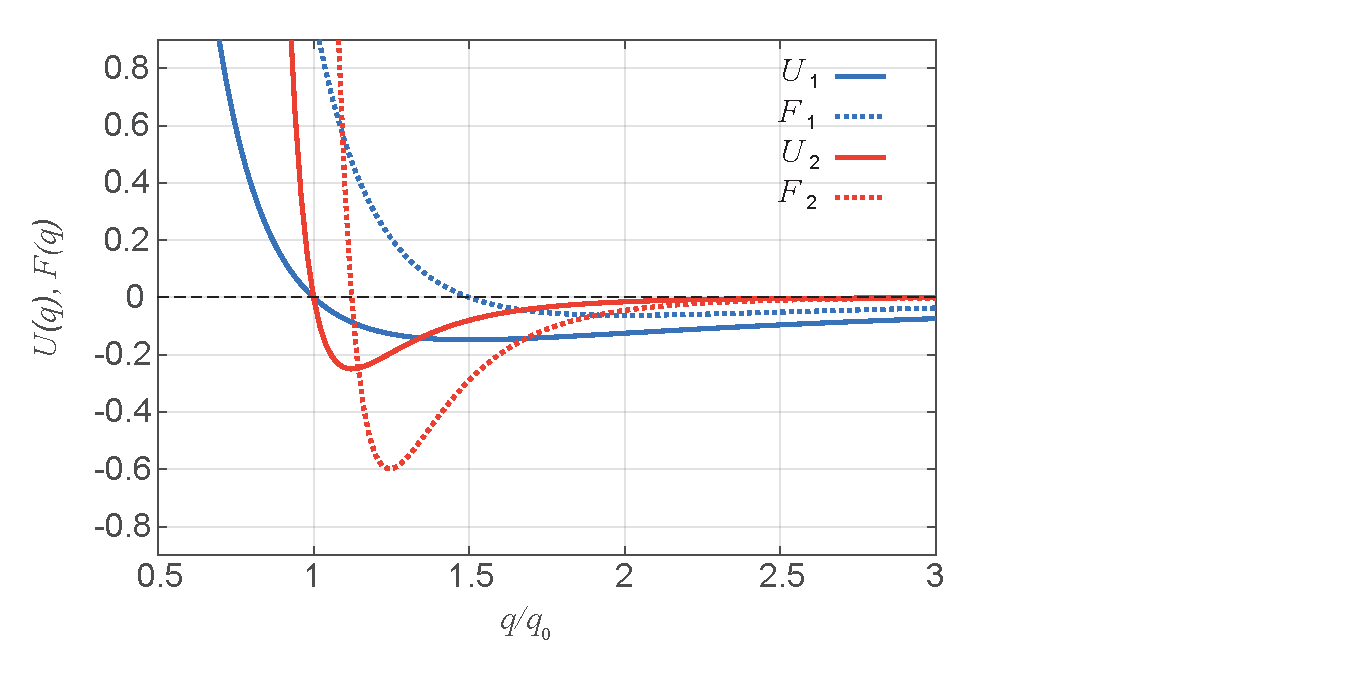
\includegraphics[width=\textwidth]{Molekuelpot01.pdf}
\caption[Potential und Kraftverlauf f�r zwei Molek�lpotentiale]{Potential- und Kraftverlauf f�r das Lennard-Jones-Potential (Index 1), sowie das Potential f�r heterogene zweiatomige Molek�le (Index 2)} 
\label{abb:bew_MolekuelPot01}
\end{figure}

\begin{figure}[H]\centering
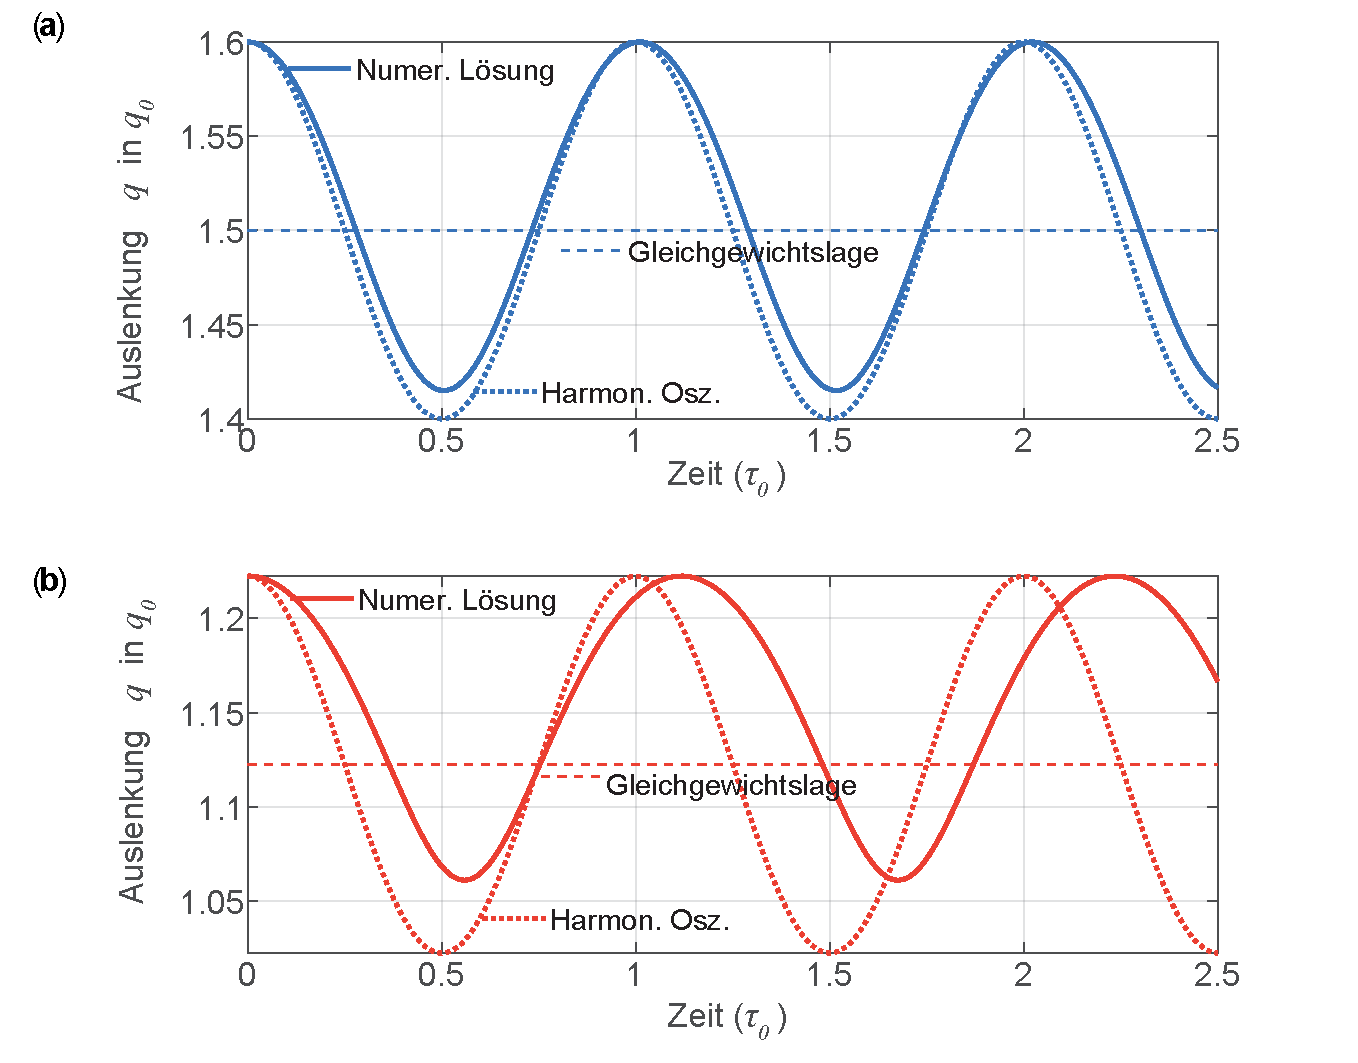
\includegraphics[width=\textwidth]{Molekuelpot02.pdf}
\caption[Schwingungsverl�ufe bei zweiatomigen Molek�len]{Schwingungsverl�ufe bei zweiatomigen Molek�len f�r das Lennard-Jones-Potential \fa und das Potential f�r ein heterogenes zweiatomiges Molek�l \fb} 
\label{abb:bew_MolekuelPot02}
\end{figure}

	\subprob{Modell f�r Nicht-Edelgas-Atome}
	H�ufig schreibt man das Potential f�r ein zweiatomiges Molek�l, das aus zwei unterschiedlichen Atomen besteht, wie folgt \cite{Timberlake2008}:
	\begin{equation}
		U(q) = \lk \frac{A}{q^3} - \frac{B}{q^2} \rk = \lk \tilde{\epsilon}_\text{A} \frac{{q_0}^3}{q^3} - \tilde{\epsilon}_\text{B} \frac{{q_0}^2}{q^2} \rk \label{eq:bew_Uebung22_04}~.
	\end{equation}
	Wir f�hren die Rechnungen analog zum ersten Aufgabenteil durch und erhalten folgende Ergebnisse:
	\begin{enumerate}[a)]
		\item Bindungsl�nge\\
			\begin{align*}
			&\frac{\partial U}{\partial q} \bigg|_{q_\text{B}} = -\frac{3A}{{q_\text{B}}^4}+ \frac{2B}{{q_\text{B}}^3} \overset{!}{=} 0  \\
			&\rightarrow q_\text{B} = \frac{3A}{2B}= \frac{3 \tilde{\epsilon}_\text{A}}{2 \tilde{\epsilon}_\text{B}} \, q_0 ~.
			\end{align*}
%\newpage
		\item Schwingungsfrequenz\\
			\begin{align}
				k_\text{eff} &= \frac{\partial^2}{\partial q^2}U(q) \bigg|_{q_\text{B}}
				= \frac{12A}{{q_\text{B}}^5}-\frac{6B}{{q_\text{B}}^4} \nonumber \\
				\rightarrow \omega^2 &= \frac{k_\text{eff}}{m_\text{eff}} = \frac{32B^5}{81 m_\text{eff}\,A^4} = \frac{32}{81} \frac{\tilde{\epsilon}_\text{B}{}^5}{\tilde{\epsilon}_\text{A}{}^4\,m_\text{eff} \, {q_0}^2}~. \label{eq:bew_Uebung22_05} 
			\end{align}
		\item Potential- und Anziehungskraftverlauf\\
			Als Vergleich zum Lennard-Jones-Potential von Aufgabenteil 1 sind in \figref{bew_MolekuelPot02} auch die Kurven f�r das Potential nach \eqref{eq:bew_Uebung22_04} berechnet und gezeigt.\\
	\end{enumerate} 

	\subprob{Zeitentwicklungen (Zusatz)}\\
		Beim Aufstellen der DGL f�r die \matlab-Routine \odevf{} haben wir folgende Vorgehensweise f�r die Zeiteichung gew�hlt.
		Die Schwingungsfrequenz ist in der harmonischen N�herung gegeben durch:
		\[ \omega_0^2 = \frac{k_\text{eff}}{m_\text{eff}} = \frac{1}{m_\text{eff}} \frac{\partial ^2}{\partial q^2}(-U) \bigg|_{q_\text{B}} ~,
		\]
		wobei $m_\text{eff}$ die effektive \bzw reduzierte Masse ist.
		Wir betrachten nun die beiden diskutierten Potentiale im Vergleich und nehmen auch vereinfachend an, dass $\tilde{\epsilon}_\text{A} = \tilde{\epsilon}_\text{B}$ ist.\\
		\begin{enumerate}[a)]
		\item Lennard-Jones-Potential\\
		F�r
		\[ U(q) = \frac{A}{q^{12}} - \frac{B}{q^6}
		\]
		mit $A= 4 \tilde{\epsilon}\,{q_0}^{12}$, $B= 4 \tilde{\epsilon}\,{q_0}^6$ und $q_\text{B} = \sqrt[6]{2}\,q_0$ ergibt sich als Schwingungsfrequenz
\begin{align}
			\omega_0^2 = \frac{72 \tilde{\epsilon}}{{q_0}^2 \,\sqrt[3]{2}\,m_\text{eff}}  \label{eq:bew_Uebung22_Z1}
\end{align}
		und entsprechend f�r die Periodendauer
		\[{T_\text{P}}^2 = \frac{\pi^2}{18} {q_0}^2 \,\sqrt[3]{2} \,\frac{m_\text{eff}}{\tilde{\epsilon}}~. \]
		Die DGL ist damit
		\[ \frac{\d}{\d t}\dot{q} = - \frac{\partial}{\partial q}U(q) = \frac{4 \pi^2}{18} \sqrt[3]{2} \,\frac{m_\text{eff}}{\tilde{\epsilon}} \lk \frac{12}{q^3} - \frac{6}{q^7} \rk~.	\]
	\item Nicht-Edelgas-Atome\\
		F�r 
		\[ U(q) = \frac{A}{q^3} - \frac{B}{q^2}
		\]
		mit $A= \tilde{\epsilon}{q_0}^3$, $B= \tilde{\epsilon}{q_0}^2$ und $q_\text{B} = \frac{3}{2} q_0$ ist die Schwingungsfrequenz
		\[{\omega_0}^2 = \frac{32}{81} \frac{\tilde{\epsilon}}{m_\text{eff}\,{q_0}^2} \]
		und die Periodendauer
		\[{T_\text{P}}^2 = \frac{81}{8} \pi^2 \,\frac{m_\text{eff}\,{q_0}^2}{\tilde{\epsilon}}~. \]
		Damit k�nnen wir die DGL schreiben als
		\[ \frac{\d}{\d t}\dot{q} = -\frac{\partial}{\partial q}U(q) = \frac{81}{8} \frac{m_\text{eff}}{\tilde{\epsilon}} \pi^2 \lk \frac{3}{q^4} - \frac{2}{q^3} \rk~.
		\]
	\end{enumerate}
		Wir erkennen, dass die gr��ere Anharmonizit�t beim Lennard-Jones-Potential auch schon bei kleinen Auslenkungen zu deutlichen Abweichungen vom Schwingungsverhalten des harmonischen Oszillators f�hrt.
		Deutlich erkennbar ist auch die gr��ere Asymmetrie in den Umkehrpunkten bedingt durch die nichtlinearen Terme in Form der h�heren Potenzen.
		Es ist sehr instruktiv, den Anfangswert $q_i$ im Programm zu ver�ndern und das Einsetzen der Anharmonizit�t zu beobachten. \\

	\subprob{Quantitative Absch�tzung (Zusatz)}
	Wir k�nnen die L�sung benutzen, um eine Absch�tzung f�r molekulare Schwingungsfrequenzen und Dissoziationsenergien nach einer klassischen Betrachtung zu erhalten.
        Wir wollen dies f�r ein Molek�l tun, das aus zwei Helium-Atomen besteht.
        F�r dieses System kann man die Parameter f�r das Lennard-Jones-Potential wie folgt annehmen:
\begin{align*}
\tilde{\epsilon}_\text{A} &= \tilde{\epsilon}_\text{B} =\SI{2.5e-22}{\J} = \tilde{\epsilon}
\qquad \text{und} \qquad q_0 =\SI{2.5e-10}{\metre}\,.
\end{align*}
	Die Tiefe des Potentialtopfes an der Stelle $q_\text{B}=\sqrt[6]{2}\,q_0$ ist aus \eqref{eq:bew_Uebung22_00} gegeben durch:
	\[
	E_\text{min} = -2 \tilde{\epsilon} = -\SI{5e-22}{\J}\,.
	\]
	In der Molekularphysik ist es �blich, Energien mittels Temperaturen eines Gleichgewichtssystems �ber 
\begin{align}
	E = k_\text{B} T \,\label{eq:bew_Uebung22_06}
\end{align}
auszudr�cken, worin $k_\text{B}= \SI{1.38064852e-23}{\J\per\K}$ die Boltzmann\footnote{Ludwig Eduard Boltzmann\indexp{Boltzmann, Ludwig Eduard} (1844--1906) war ein bedeutender �sterreichischer Physiker und arbeitete vor allem auf den Gebieten der Thermodynamik und der statistischen Mechanik.}-Konstante und $T$ die Temperatur in $\SI{}{\K}$ ist.
Demnach entspricht die Tiefe des Potentialtopfes gerade einmal einer Temperatur von $ T \approx \SI{18}{\K}$.
Da das Lennard-Jones-Potential auf seinem Definitionsbereich nur dieses eine Minimum besitzt und f�r $R \rightarrow\infty$ gegen Null geht, handelt es sich hierbei wirklich um die \anf{tiefste} Stelle des Potentials und nach der klassischen Mechanik w�re das auch die Bindungsenergie.
In der Quantenmechanik hat ein System nicht die minimale Energie eines Potentials, sondern besitzt immer mindestens eine sogenannte Nullpunktsenergie \cite{Schmutzer2005, Bartelmann2015}.
Diese Nullpunktsenergie kann man anschaulich als etwa die minimale relative Schwingung beider Heliumatome ansehen, die durch das Lennard-Jones-Potential erlaubt wird.
Die Frequenz dieser Schwingung hatten wir in \eqref{eq:bew_Uebung22_Z1} hergeleitet, woraus sich ergibt:
	\[\omega_0 = \SI{8.29e12}{\per\s} \quad \text{\bzw} \quad T_\text{P} = \SI{7.58e-13}{\s}\,.
\]
Die Energie einer solchen Schwingung ist nach der Quantentheorie durch $\frac{1}{2} \hbar\omega_0$ gegeben und berechnet sich damit zu:
	\[E_0 = \SI{4.37e-22}{\J} \quad \text{\bzw} \quad  T_0 = \SI{31.7}{\K}\,.
\]
Dieser Wert liegt signifikant oberhalb der maximalen Tiefe von 18\,K des Lennard-Jones-Potentials, sodass mit den angenommenen Werten f�r $q_0$ und $\tilde{\epsilon}$ keine stabilen
Heliummolek�le zu erwarten sind (zumindest nicht im Grundzustand), vielmehr werden diese, so sie sich irgendwie transient gebildet haben, sofort (d.h. ungef�hr in der Zeit $T_\text{P}$) dissoziieren.\footnote{In Experimenten mit ultrakaltem Helium \cite{Grisenti2000} hat man die Bindungsenergie $E_\text{B} = E_\text{min} + E_0$ zu ca. $\SI{1.1e-03}{\K}$ und den Bindungsradius zu $\SI{5.2e-09}{\metre}$ bestimmt, was ein extrem schwach gebundenes Molek�l darstellt.
Wir haben also in unserem einfachen Modell den Atomabstand massiv untersch�tzt.}
\end{subprobs}
\end{sol} 
%\href{PhysikUncut_Part1.pdf#prb:bew_Molekuelpotentiale}{\textcolor{blue} {$\rightarrow$ zur \probref{bew_Molekuelpotentiale}.}}\\
\textcolor{blue} {$\rightarrow$ zur} \probref{bew_Molekuelpotentiale}.\\
\noindent\rule[1ex]{\textwidth}{0.5pt}  \newpage

%-----------------------------------------------------------------------------------------------------------

\hypertarget{lsg:bew_Kopplung01}{}
\begin{sol}{prob:bew_Kopplung01}\label{lsg:bew_Kopplung01}%�bung28
\textbf{Zwei gekoppelte Stangenpendel.} \\ \\
Wir benutzen die Geometrie aus \figref{bew_Kopplg01}.
Wir kommen auf folgende Bewegungsgleichungen:
\begin{align}
		\ddot{\theta}_1 + {\omega_{\uproman{1}}}^2\sin\theta_1 + \kappa_{\uproman{1}}\, \lk \sin\theta_1-\sin\theta_2\rk \,\cos\theta1  &= 0 \,,\nonumber \\
		\ddot{\theta}_2 + {\omega_{\uproman{2}}}^2\sin\theta_2 - \kappa_{\uproman{2}}\, \lk \sin\theta_1-\sin\theta_2\rk \,\cos\theta2  &= 0 \,. \label{eq:bew_LsgKopplung01a}
\end{align}
Mit den N�herungen f�r kleine Winkel gilt:
\begin{align}
		\ddot{\theta}_1 + {\omega_{\uproman{1}}}^2\theta_1 + \kappa_{\uproman{1}}\, \lk \theta_1-\theta_2\rk &= 0 \,,\nonumber \\
		\ddot{\theta}_2 + {\omega_{\uproman{2}}}^2\theta_2 - \kappa_{\uproman{2}}\, \lk \theta_1-\theta_2\rk &= 0 \,. \label{eq:bew_LsgKopplung01}
\end{align}
Hier haben wir die Eigenfrequenzen 
\begin{equation*}
	\omega_\text{I}^2 = \frac{g}{l_{1}} 
	\qquad \text{und} \qquad 
	\omega_\text{II}^2 = \frac{g}{l_{2}}
\end{equation*}
sowie die effektiven Kopplungskonstanten
\begin{equation*}
	\kappa_{\uproman{1}} = \frac{\kappa\,{l_\text{F}}^2}{m_{1}\,{l_{1}}^2} \,\\
	\qquad \text{und} \qquad 
	\kappa_{\uproman{2}} = \frac{\kappa\,{l_\text{F}}^2}{m_{2}\,{l_{2}}^2}
\end{equation*}
verwendet. 
Die L�sung der charakteristischen Gleichung \eqref{eq:bew_Kopplg08} f�hrt f�r $\lambda_{1/2} = {\omega_{1/2}}^2$ auf die folgende Schwingungsfrequenzen:
\begin{align}
		{\omega_{1/2}}^2 &= \frac{{\omega_{\uproman{1}}}^2 + {\omega_{\uproman{2}}}^2 + \kappa_1 + \kappa_2}{2}\nonumber \\
		&\quad \pm \frac{1}{2} \sqrt{\lk {\omega_{\uproman{1}}}^2-{\omega_{\uproman{2}}}^2\rk^2 + \lk \kappa_1+\kappa_2 \rk^2+ 2\lk {\omega_{\uproman{1}}}^2 -{\omega_{\uproman{2}}}^2\rk \lk \kappa_1-\kappa_2\rk}\,.\label{eq:bew_LsgKopplung02}
\end{align}
Man beachte, dass hierin $\omega_1$ und $\omega_2$ die Normalfrequenzen des gekoppelten Systems darstellen, hingegen $\omega_{\uproman{1}}$ und $\omega_{\uproman{2}}$ die Eigenfrequenzen der einzelnen Pendel.
Wir widmen uns nun den konkreten Teilaufgaben mit den Angaben f�r die Pendell�ngen.
\begin{subprobs}
	\subprob{Pendel mit gleicher L�nge und Masse, kleine Winkel}
	Hier gilt $l_1 = l_2$ und $m_1 = m_2$.
	Au�erdem verwenden wir die Anfangsbedingungen 
	$\theta_1\lk 0\rk = \theta_0$, 
	$\theta_2\lk 0\rk = 0$, sowie
	$\dot{\theta}_{10}= 0$ und $\dot{\theta}_{20}= 0$.
	Dann erhalten wir mit $\kappa_1=\kappa_2=\kappa$ und $\omega_{\uproman{1}} = \omega_{\uproman{2}} = \omega_0$ als Frequenzen der Eigenschwingungen der beiden Pendel 
	\begin{align*}
			\omega_1  &= \omega_0 \,, \\
			\omega_2 &= \sqrt{{\omega_0}^2 + 2\kappa}\,.
	\end{align*}
	Die Normalschwingungen sind durch $\begin{pmatrix} 1 \\ 1 \end{pmatrix}$ \bzw $\begin{pmatrix} -1 \\ 1 \end{pmatrix}$ gegeben. 
	Wir wollen nun den Fall betrachten, dass ein Pendel zur Startzeit eine Auslenkung $\theta_{10}$ hat, wohingegen alle anderen Anfangsbedingungen Null sind. 
	Dann ergibt sich mit $C = \frac{\theta_0}{2}$ 
	\begin{align*}
			\theta_1 &= C\lk \cos\omega_1t + \cos\omega_2t\rk \,, \\
			\theta_2 &= C\lk \cos\omega_1t - \cos\omega_2t\rk\,.
	\end{align*}
	Man erkennt, dass die Auslenkungen $\theta_1$ , $\theta_1$ wegen der gleichen Kopplungskonstante, also wegen $\kappa_1 = \kappa_2$, reine Schwebungen darstellen.

\begin{figure}[H]\centering
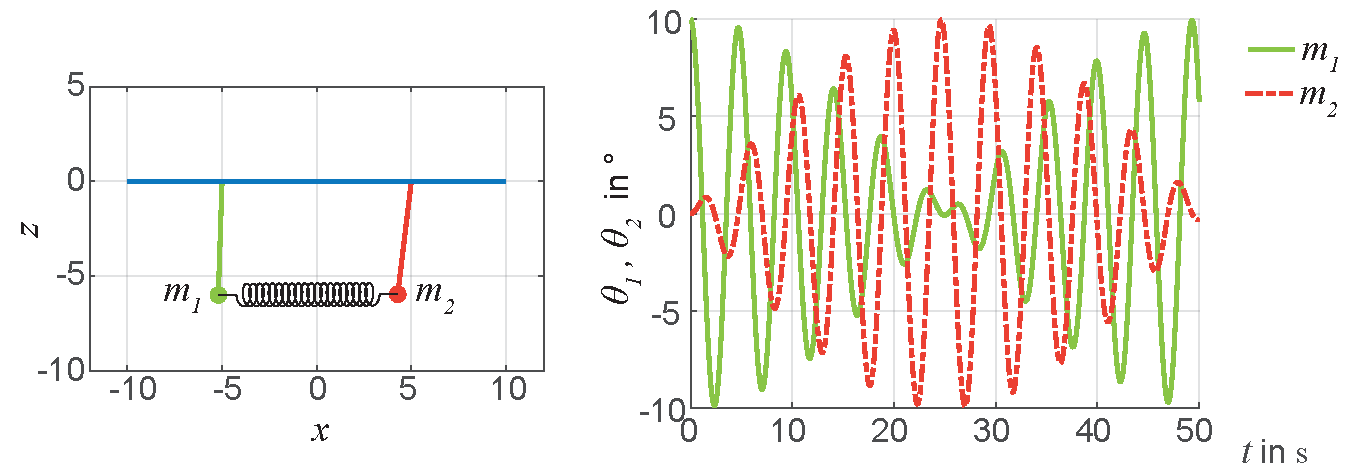
\includegraphics[width=\textwidth]{LsgGekopPendel01.pdf}%
\caption[Kleinwinkel-Schwingungsverhalten zweier gekoppelter Stangenpendel]{Kleinwinkel-Schwingungsverhalten zweier miteinander gekoppelter Stangenpendel gleicher L�nge und Masse. Deutlich ist das Schwebungsverhalten zu erkennen, \vgl \mlbewref{GekoppeltePendel01.m}. Parameter: $l_1 = l_2= \SI{6}{\metre}, m_1 = m_2 = \SI{3}{\kg}, D = \SI{0.5}{\N\per\metre}, \theta_{10} = 10\degree, \theta_{20} = 0\degree$ und $l_F = \SI{6}{\metre}$}
\label{abb:bew_LsgKopplung01}
\end{figure}

	\subprob{Pendel mit ungleicher L�nge, kleine Winkel}
	Hier gilt nun 
	$l_1 \neq l_2 \neq l_\text{F}$ und $m_1 \neq m_2$.
        Als Anfangsbedingungen verwenden wir die gleichen wie oben.
	Durch analoges Vorgehen erhalten wir
	\begin{align}
		{\omega_{1/2}}^2 &= \frac{{\omega_{\uproman{1}}}^2 + {\omega_{\uproman{2}}}^2 + \kappa_1 + \kappa_2}{2}\nonumber \\
		&\quad \pm\frac{1}{2}\lk {\omega_{\uproman{1}}}^2 - {\omega_{\uproman{2}}}^2\rk\sqrt{1+2\frac{\kappa_1-\kappa_2}{{\omega_{\uproman{1}}}^2-{\omega_{\uproman{2}}}^2}+\lk \frac{\kappa_1+\kappa_2}{{\omega_{\uproman{1}}}^2-{\omega_{\uproman{2}}}^2}\rk^2   }\,.
		\label{eq:bew_LsgKopplung03}
	\end{align}
	F�r kleinere Kopplungsst�rken, d.h. f�r $\kappa_1 \pm \kappa_2 \ll {\omega_{\uproman{1}}}^2-{\omega_{\uproman{2}}}^2$ kann man die Wurzel als Reihe entwickeln. (Das geht offensichtlich nicht, wenn ${\omega_{\uproman{1}}}^2 \approx {\omega_{\uproman{2}}}^2$, aber eben diesen Fall haben wir ja in Teilaufgabe 1 behandelt).
	Wir erhalten als Normalfrequenzen
	\begin{align*}
		{\omega_1}^2 &= {\omega_{\uproman{1}}}^2 + \kappa_1 + \frac{\kappa_1\kappa_2}{{\omega_{\uproman{1}}}^2-{\omega_{\uproman{2}}}^2} \,, \\
		{\omega_2}^2 &= {\omega_{\uproman{2}}}^2 + \kappa_2 -\frac{\kappa_1\kappa_2}{{\omega_{\uproman{1}}}^2-{\omega_{\uproman{2}}}^2} \,.
	\end{align*}
	und k�nnen damit auch die entsprechenden Schwingungen analytisch berechnen. 
	F�r die vorgegebenen Randbedingungen erhalten wir:
	\begin{align*}
		\theta_1 &= \frac{\theta_{10}}{C_1-C_2} \lk C_1\cos\omega_1 t - C_2\cos\omega_2 t\rk \,, \\
		\theta_2 &= \frac{\theta_{10}}{C_1-C_2} \lk \cos\omega_1 t - \cos\omega_2 t\rk \,, \\
	\end{align*}
	worin 
		\[C_1 = \frac{\omega_{\uproman{2}}^2-{\omega_1}^2 + \kappa_2}{\kappa_2}~~\text{und}~~C_2 = \frac{\omega_{\uproman{2}}^2-{\omega_2}^2 + \kappa_2}{\kappa_2}
	\]
	sind.
        Man erkennt, dass $\theta_1$ auch hier keine reine Schwebung mehr darstellt.
	Es ist also schon jetzt sehr vorteilhaft, das Problem numerisch anzugehen.
        Wir haben dies in \mlbewref{GekoppeltePendel02.m} getan.

\begin{figure}[H]\centering
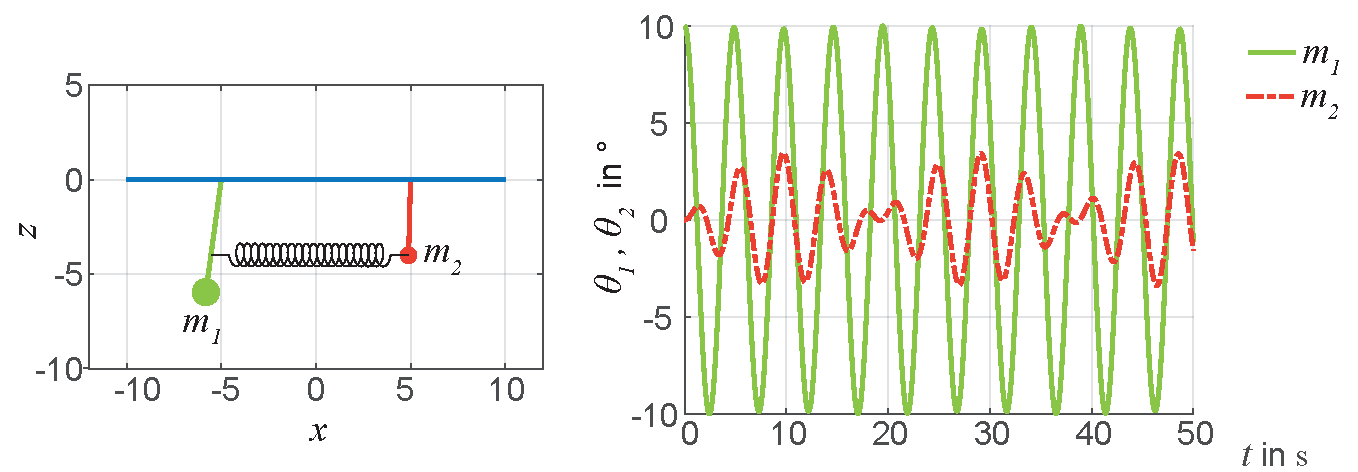
\includegraphics[width=\textwidth]{LsgGekopPendel02.pdf}%
\caption[Kleinwinkel-Schwingungsverhalten zweier gekoppelter Stangenpendel]{Kleinwinkel-Schwingungsverhalten zweier miteinander gekoppelter Stangenpendel unterschiedlicher L�nge. Deutlich ist das Schwebungsverhalten f�r $\theta_2$ zu erkennen, w�hrend $\theta_1$ keine Schwebung mehr darstellt. Parameter: $l_1 = \SI{6}{\metre}, 
l_2 = \SI{4}{\metre}, m_1 = \SI{5}{\kg}, m_2 = \SI{3}{\kg}, D2 = \SI{0.5}{\N\per\metre}, \theta_{10} = 10\degree, \theta_{20} = 0\degree$ und $l_F = \SI{4}{\metre}$}
\label{abb:bew_LsgKopplung02}
\end{figure}

	\subprob{Beliebig gro�e Auslenkungen und unterschiedlich lange Pendel}
	Die L�sung ist in \mlbewref{GekoppeltePendel03.m} ausgef�hrt.\\
		
\begin{figure}[H]\centering
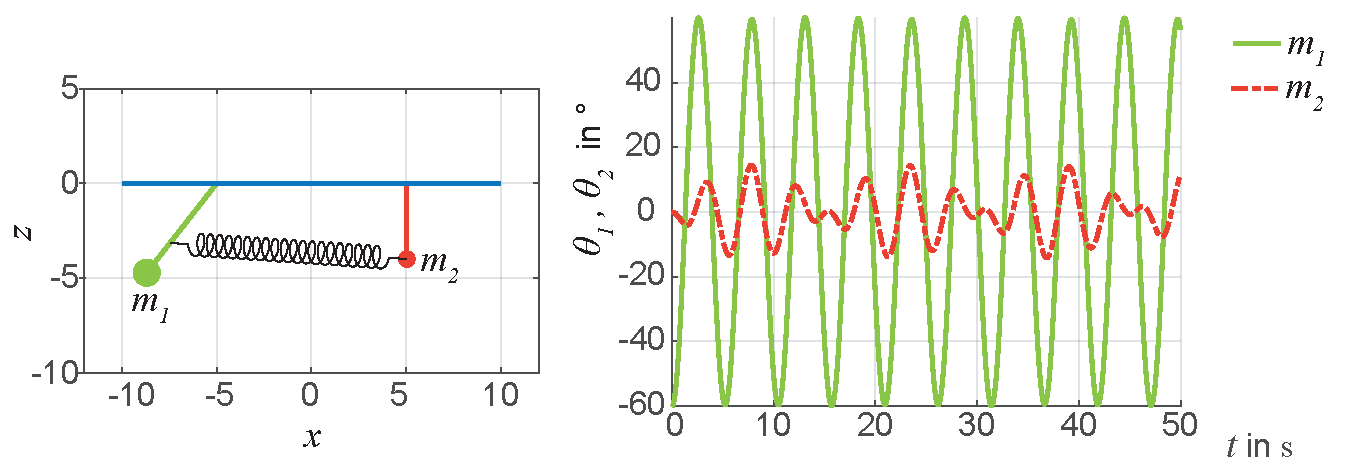
\includegraphics[width=\textwidth]{LsgGekopPendel03.pdf}%
\caption[Schwingungsverhalten zweier gekoppelter Stangenpendel]{Schwingungsverhalten zweier miteinander gekoppelter Stangenpendel. Parameter: $l_1 = \SI{6}{\metre}, l_2 = \SI{4}{\metre}, m_1 = \SI{5}{\kg}, m_2 = \SI{3}{\kg}, D2 = \SI{0.5}{\N\per\metre}, \theta_{10} = 60\degree, \theta_{20} = 0\degree$ und $l_F = \SI{4}{\metre}$}
\label{abb:bew_LsgKopplung03}
\end{figure}

\end{subprobs}

\end{sol} 
%\href{PhysikUncut_Part1.pdf#prb:bew_Kopplung01}{\textcolor{blue} {$\rightarrow$ zur \probref{bew_Kopplung01}.}}\\
\textcolor{blue} {$\rightarrow$ zur} \probref{bew_Kopplung01}.\\
\noindent\rule[1ex]{\textwidth}{0.5pt}  \newpage


%-----------------------------------------------------------------------------------------------------------

\hypertarget{lsg:bew_CO2Molekuel}{}
\begin{sol}{prob:bew_CO2Molekuel}\label{lsg:bew_CO2Molekuel} %%�bung29
\textbf{Schwingungen des  $\text{CO}_2$-Molek�ls} \\
\begin{subprobs}
\subprob{Streckschwingungen des Molek�ls}
In der \probref{bew_Molekuelpotentiale} Molek�lpotentiale hatten wir Approximationen der tats�chlichen Kr�fte zwischen den Atomen gefunden, die zu einem nichtlinearen Verhalten f�hrten. 
Wir werden am Ende dieser �bung noch auf diese eingehen, wollen uns aber zun�chst auf den einfachen Fall der harmonischen N�herung beschr�nken. Wir modellieren das CO$_2$-Molek�l zun�chst als \emph{linearen} Federschwinger, beschreiben die Kraft also in der N�herung $\keff\, x$. 
Als Lagrange-Funktion ergibt sich damit 
\begin{align}
    \mathcal{L} &= T -U \nonumber \\
    &= \frac{m_\text{O}^2}{2}\lk \dot{x_1}^2  + \dot{x_3}^2 \rk + \frac{m_\text{C}}{2}\dot{x_2}^2 - \frac{\keff}{2} \lk (x_2 - x_1 - L)^2 + (x_3 - x_2 - L)^2\rk
    \label{eq:bew_CO2M01}~.
\end{align}
Wir setzen  $q_1 = x_1 - L$, $q_2 = x_2$ und $q_3 = x_3 - L$.
Mit diesen generalisierten Koordinaten 
\begin{equation}
    \vec{q} = 
    \begin{pmatrix}
    	q_1 \\ q_2 \\ q_3
    \end{pmatrix}
    \label{eq:bew_CO2M02}
\end{equation}
k�nnen wir $T$ und $U$ mit den Matrizen $\mathbb{T}$ und $\mathbb{U}$ folgenderma�en schreiben:
\begin{align}
    T &= \frac{1}{2} \dot{\vec{q}}^T \mathbb{T} \dot{\vec{q}}
    \qquad &\text{mit} \qquad
    \mathbb{T} &= 
    \begin{pmatrix}
        m_\text{O} & 0 & 0 \\
        0 & m_\text{C} & 0 \\
        0 & 0 & m_\text{O}
    \end{pmatrix} \nonumber \\
    U &= \frac{\keff}{2} \sum_{i,j = 1}^3 q_i q_j U_{ij}
    \qquad &\text{mit} \qquad 
    \mathbb{U} &= \keff
    \begin{pmatrix}
        1 & -1 & 0 \\
        -1 & 2 & -1 \\
        0 & -1 & 1
    \end{pmatrix}~.
    \label{eq:bew_CO2M03}
   \end{align} 
   W�hrend die Matrix der kinetischen Energie $\mathbb{T}$ diagonalisiert ist, zeigen die Nebendiagonalelemente von $\mathbb{U}$, dass die Schwingungen gekoppelt sind.
   Die generalisierten Koordinaten $q_1$ und $q_3$ sind entkoppelt, f�r die urspr�nglichen Koordinaten $x_1$ und $x_3$ w�rde das nicht gelten.
   Wir bestimmen die Eigenwerte $\lambda$ aus der charakteristischen Gleichung \eqref{eq:bew_Kopplg08}: 
   \begin{equation}
       \det(\mathbb{U} - \lambda \mathbb{T}) = 
       \begin{vmatrix}
           \keff-\lambda\,m_\text{O} & -\keff & 0 \\
           -\keff & 2 \keff - \lambda\,m_\text{C} & - \keff \\
           0 & -\keff & \keff - \lambda\, m_\text{O}
       \end{vmatrix}
       = 0 
       \label{eq:bew_CO2M04}
   \end{equation}
   und erhalten die in $\lambda$ kubische Gleichung
   \begin{equation}
        (\keff - \lambda\, m_\text{O}) \lek (2 \keff - \lambda\, m_\text{C})(\keff -\,\lambda\, m_\text{O}) - {\keff}^2 \rek
        - {\keff}^2 \,(\keff - \lambda\,m_\text{O}) = 0~.
        \label{eq:bew_CO2M05}
    \end{equation} 
    Man findet damit
    \begin{align}
        \lambda_1 &= \frac{\keff}{m_\text{O}} = {\omega_{1,0}}^2 > 0 \nonumber \\
        \lambda_2 &= \lk \frac{\keff}{m_\text{O}} + \frac{2 \keff}{m_\text{C}} \rk = {\omega_{2,0}}^2 > 0 \nonumber \\
        \lambda_3 &= 0 \label{eq:bew_CO2M06}~.
    \end{align}
    Die Eigenwerte $\lambda_1$ und $\lambda_2$ sind verschieden von 0 und ergeben Schwingungsfrequenzen f�r Eigenschwingungen, w�hrend $\lambda_3 = 0$ bedeutet, dass hier eine reine Translation vorliegt.
    Wir bestimmen die beiden Eigenschwingungen nach \eqref{eq:bew_Kopplg07} zun�chst f�r $\lambda_1$:
    \begin{equation}
        (\mathbb{U} - \lambda_1 \mathbb{T}) \vec{n}_1 = 
        \begin{pmatrix}
            0 & -\keff & 0 \\
            -\keff ~~~& \keff \lk2-\frac{m_\text{C}}{m_\text{O}}\rk ~~~& -\keff \\
            0 & -\keff & 0
        \end{pmatrix}
        \begin{pmatrix}
            n_{1,1} \\ n_{1,2} \\ n_{1,3}
        \end{pmatrix}
        = 0~, \label{eq:bew_CO2M07}
    \end{equation}
    wobei wir der Einfachheit halber durch $m_\text{O}$ dividiert haben.
    Daraus folgt $n_{1,2} = 0$  und $n_{1,3} = -n_{1,1}$, \bzw
    \begin{equation}
        \vec{n}_1 = C
        \begin{pmatrix}
            1 \\ 0 \\ -1
        \end{pmatrix}
        \label{eq:bew_CO2M08}~.
    \end{equation}
    Den Vorfaktor bestimmen wir aus der Forderung nach Normierung der Eigenschwingung
		\[	{\vec{n}_i}^T ~ \mathbb{T} ~ \vec{n}_j = \delta_{ij}
\] 	 zu $C = \frac{1}{\sqrt{2m_\text{O}}}$. 
    Analog erh�lt man f�r den zweiten Eigenwert  $\lambda_2$ den Eigenvektor:
    \begin{equation}
        \vec{n}_2 = \sqrt{\frac{m_\text{C}}{2m_\text{O} (2m_\text{O}+m_\text{C})}} 
        \begin{pmatrix}
            1 \\ -2m_\text{O}/m_\text{C} \\1
        \end{pmatrix} \,.
        \label{eq:bew_CO2M09}
    \end{equation}
    F�r den dritten Eigenwert finden wir:
    \begin{equation}
        \vec{n}_3 = \sqrt{\frac{1}{2m_\text{O} +m_\text{C}}} 
        \begin{pmatrix}
            1 \\ 1 \\1
        \end{pmatrix}
        \label{eq:bew_CO2M10}~.
    \end{equation}
    Zur Berechnung kann man die \matlab{} Symbolic Toolbox verwenden.
    Interessant ist, dass die Eigenfrequenzen von $\keff$, $m_\text{O}$ und $m_\text{C}$ abh�ngen, die Eigenvektoren hingegen nur von den Massen.
    Wie man an \eqref{eq:bew_CO2M08} erkennt, entspricht die Eigenschwingung $\vec{n}_1$ einer antisymmetrischen (!) Schwingung der Sauerstoff-Atome.
    Das Kohlenstoff-Atom bleibt allerdings in Ruhe. Dies wird symmetrische (!) Streckschwingung (\figref{bew_CO2Molekuel02}\,a) genannt.\footnote{Gezielte Verwirrung ist manchmal Teil des Physik-Curriculums.}
    Bei $\vec{n}_2$ schwingen die Sauerstoff-Atome gleichphasig, aber das Kohlenstoff-Atom gegenphasig zu diesen. Man spricht hier von einer antisymmetrischen (!) Streckschwingung (\figref{bew_CO2Molekuel02}\,b).
    Der Eigenvektor $\vec{n}_3$ beschreibt eine Bewegung des Gesamtsystems entlang der $x$-Achse (Translation) und bedeutet gerade die Gesamtimpulserhaltung.
    Damit ist die Gesamtbewegung
    \begin{equation}
        \vec{q}(t) = 
        \begin{pmatrix}
            q_1(t) \\ q_2(t) \\ q_3(t)
        \end{pmatrix}
        =
        \begin{pmatrix}
        \vec{n}_1 A_1 \cos(\omega_{1,0}t -\delta_1) \\
        \vec{n}_2 A_2 \cos(\omega_{2,0}t -\delta_2) \\
        \vec{n}_3 (q_{3,0} + \dot{q}_{3,0})
        \end{pmatrix},
        \label{eq:bew_CO2M11}
    \end{equation}
    wobei sich die Konstanten $A_1$, $A_2$, $\delta_1$ und $\delta_2$ aus den Anfangsbedingungen ergeben, genauso wie die $q_{3,0} = q_3(t=0)$ und $\dot{q}_{3,0} = \dot{q}_3(t=0)$.
    In kartesischen Koordinaten erh�lt man durch R�cksubstitution
    \begin{equation}
        \vec{x}(t) = 
        \begin{pmatrix}
            x_1(t) \\ x_2(t) \\ x_3(t)
        \end{pmatrix}
        =
        \begin{pmatrix}
            q_1(t) - L \\ q_2(t) \\ q_3(t)+L
        \end{pmatrix}
        \label{eq:bew_CO2M12}.
    \end{equation}
    Wir wollen nun noch kurz betrachten, wie die Schwingen f�r realistischere Molek�l\-potentiale aussehen.
    Wir hatten diese schon in \probref{bew_Molekuelpotentiale}
    berechnet und in der linearen N�herung f�r die Federkonstante folgendes erhalten:
    \begin{equation}
        \keff = \frac{\partial^2}{\partial q^2} U(q) \big|_{q_B} 
        = \frac{32}{81} \frac{\varepsilon}{{q_0}^2}.
    \end{equation}
    Darin waren $\varepsilon$ und $q_0$ molekulare Parameter. 
    Wir kommen damit in der harmonischen N�herung nat�rlich wieder auf die Eigenschwingungen \eqref{eq:bew_CO2M11}, im anharmonischen Fall mit den Molek�l\-potentialen k�nnen wir das System nur noch numerisch l�sen.
    %Die Ergebnisse sind f�r zwei verschiedene Anfangsbedingungen in \figref{bew_CO2Molekuel03} gezeigt.
    %Man erkennt, dass bei kleinen Auslenkungen die Eigenschwingungen erhalten bleiben (wie zu erwarten war) und das Ergebnis gut mit der harmonischen N�herung \eqref{eq:bew_CO2M11} �bereinstimmt. 
    %Bei gr��eren Auslenkungen entstehen zus�tzlichen Frequenzen (ebenfalls erwartet!), wie man sch�n am Frequenzspektrum sieht.\\
\subprob{Deformationsschwingungen des Molek�ls}
	Wir wollen jetzt noch die sogenannte Deformations- und Knickschwingung des Molek�ls modellieren.
        Dies sind Schwingungen senkrecht zur Hauptachse des Molek�ls.
    Da wir als Gleichgewichtslage das gestreckte Molek�l auf der $x$-Achse annehmen, k�nnen wir die Bewegungen in $x$- und $y$-Richtung vollst�ndig entkoppeln.
    F�r die $y$-Richtung ergeben sich die einfachen Energien
    \begin{align}
        T &= \frac{m_\text{O}}{2} \lk {\dot{y}_1}{}^2 + {\dot{y}_3}{}^2 \rk \nonumber \\
        U &= \frac{\keff}{2} \lek (y_2-y_1)^2 + (y_3-y_2)^2 \rek
        \label{eq:bew_CO2M13}~.
    \end{align}
    Sowohl die $\mathbb{T}$-, als auch die $\mathbb{U}$-Matrix sind dann identisch mit denen nach \eqref{eq:bew_CO2M03}, da wir hier einfach $q_i = y_i$ setzen k�nnen.
    Wir erhalten damit die gleichen Eigenvektoren und k�nnen sofort die L�sung aufschreiben:
    \begin{equation}
        \vec{y}(t) =
        \begin{pmatrix}
            y_1(t) \\ y_2(t) \\y_3(t)
        \end{pmatrix} =
        \begin{pmatrix}
            q_1(t) \\q_2(t) \\q_3(t)
        \end{pmatrix} =
    \begin{pmatrix}
        \vec{n}_1 A_1 \cos(\omega_{1,0}t - \delta_1) \\
        \vec{n}_2 A_2 \cos(\omega_{2,0}t - \delta_2) \\
        \vec{n}_3 (q_{3,0} + \dot{q}_{3,0})
    \end{pmatrix}.
    \end{equation}
    Die Interpretation ist allerdings hier eine andere: Die Normalschwingung $\vec{n}_1$ ist eine Art Rotation, die Normalschwingung $\vec{n}_2$ ist die sogenannte symmetrische Knickschwingung (\figref{bew_CO2Molekuel02}\,c) und $\vec{n}_3$ ist wiederum eine Translation, diesmal in $y$-Richtung. Wir wollen noch darauf hinweisen, dass man bei der Zuordnung unterschiedlicher Ladungsverteilungen auf die einzelnen Atome bei der antisymmetrischen Streckschwingung und bei der Knickschwingung eine �nderung des Dipolmoments des Molek�ls bekommt. Deswegen kann man diese Schwingungen im Infrarot-Bereich sehen.
\begin{figure}
\centering
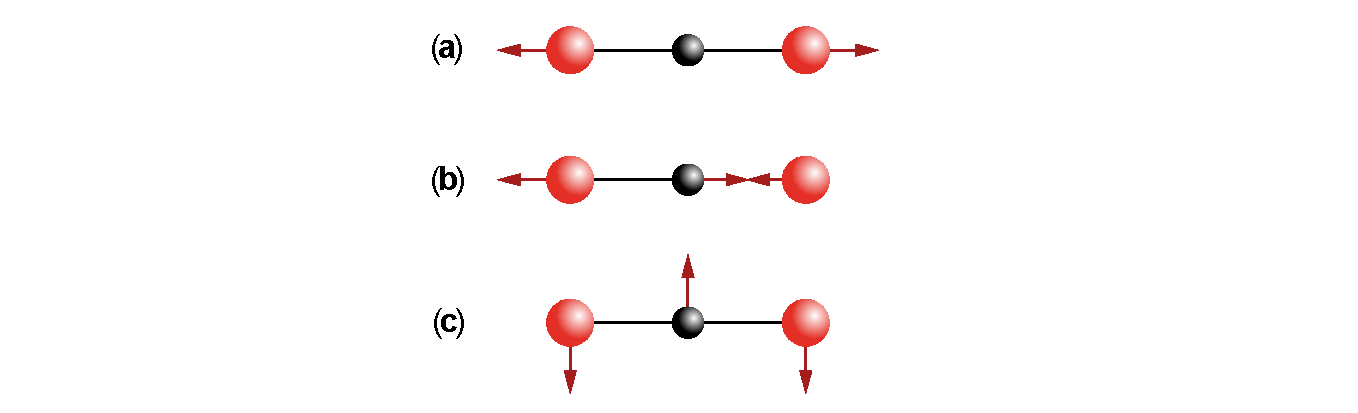
\includegraphics[width=0.9\textwidth]{CO2Molekuel02.pdf}%
\caption[Schwingungsmoden eines dreiatomigen Molek�ls ($\text{CO}_2$-Molek�l)]{Schwingungsmoden eines dreiatomigen Molek�ls. \fa Symmetrische Streckschwingung \fb Antisymmetrische Streckschwingung \fc Knickschwingung}
\label{abb:bew_CO2Molekuel02}
\end{figure}
%
%\begin{figure}[H]\centering
%
\includegraphics[width=\textwidth]{Platzhalter.pdf}%
%\caption[Asymmetrische Streckschwingung eines dreiatomigen Molek�ls ($\text{CO}_2$-Molek�l) f�r verschiedene Auslenkungen und Frequenzspektrum.]{Simulation der asymmetrischen Streckschwingung eines dreiatomigen Molek�ls ($\text{CO}_2$-Molek�l) f�r verschiedene Auslenkungen und Frequenzspektrum.(\mlbewref{MolekschwingungCO2.m}.}
%\label{abb:bew_CO2Molekuel03}
%\end{figure}
%
\end{subprobs}
\end{sol} 
%\href{PhysikUncut_Part1.pdf#prb:bew_CO2Molekuel}{\textcolor{blue} {$\rightarrow$ zur \probref{bew_CO2Molekuel}.}}\\
\textcolor{blue} {$\rightarrow$ zur} \probref{bew_CO2Molekuel}.\\
\noindent\rule[1ex]{\textwidth}{0.5pt}  \newpage


%-----------------------------------------------------------------------------------------------------------
\hypertarget{lsg:bew_Stossdaempfer}{}
\begin{sol}{prob:bew_Stossdaempfer} \label{lsg:bew_Stossdaempfer} %�bung30
\textbf{Sto�d�mpfer, Schwingungstilgung f�r Tische und in Hochh�usern.} \\ \\
Wir k�nnten nat�rlich alle drei Teilaufgaben mit den in Kap.~\ref{kap:bew_Tilgung} gezeigten Methoden l�sen, dies sei auch dem Leser zur zus�tzlichen �bung empfohlen. Wir wollen hier aber auch jeweils auf das vorliegende Problem eine spezifische auch f�r die numerische Berechnung geeignete L�sungsmethode zeigen.
\begin{subprobs}
	\subprob{Sto�d�mpfer eines Autos}
	Die Aufgabe von Sto�d�mpfern ist es, die Schwingungen des gefederten Fahrzeugs (\zb beim Durchfahren eines Schlaglochs) entsprechend zu d�mpfen.
  Dabei soll insbesondere vermieden werden, dass es zu Schwingungen im Bereich der Eigenfrequenzen (und damit m�glicherweise zur sogenannten \anf{Resonanzkatastrophe}) kommt. 	Oft wird irrt�mlicherweise angenommen, dass der Sto�d�mpfer die Fahrbahnunebenheiten abf�ngt, das ist jedoch Aufgabe der Federung. Die Feder muss die dadurch gespeicherte Energie aber wieder abgeben. Das passiert �ber Schwingungen, die �ber die Kolbenstange auf den Sto�d�mpfer �bertragen werden. Die Bewegungsenergie wird dabei durch hydraulische Widerst�nde innerhalb des Sto�d�mpfers in W�rme umgewandelt. Das Funktionsprinzip des einfachen Einrohr-Sto�d�mpfers ist in \figref{bew_Stossdaempfer02} gezeigt.

\begin{figure}
\centering
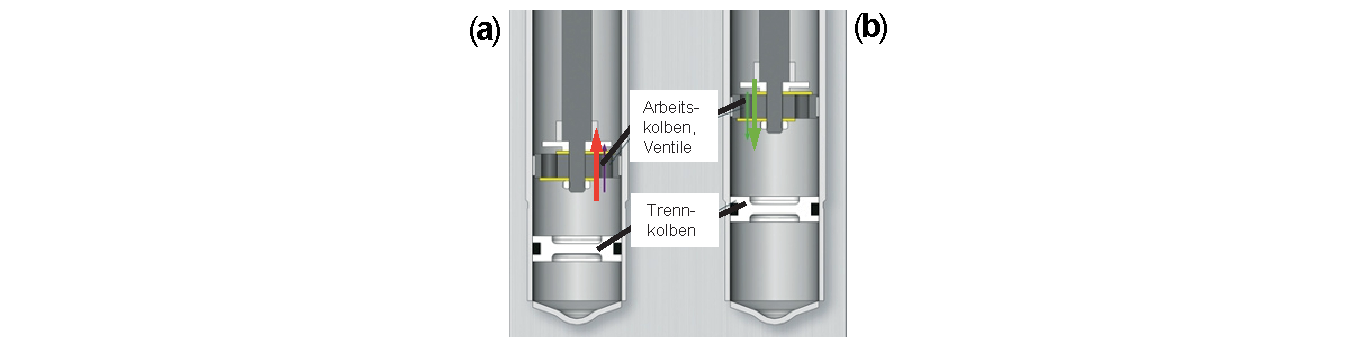
\includegraphics[width= 0.9\textwidth]{Stossdaempfer02.pdf}%
\caption[Prinzip und Aufbau eines Stossd�mpfers]{ \fa Prinzip des Sto�d�mpfers \fb Aufbau eines Einrohr-Sto�d�mpfers 
(\href{https://www.tunero.de/service/funktion-sportdaempfer.html}{https://www.tunero.de/service/funktion-sportdaempfer.html}).
Schwingt das Fahrzeug nach unten zur Fahrbahn hin, wird der Arbeitskolben des Sto�d�mpfers nach unten gedr�ckt (Bild links).
Ein Ventil setzt dem �l, das aus der unteren Kammer nach oben str�mt (roter Pfeil), einen Widerstand entgegen und bremst somit die Abw�rtsbewegung.
Der Trennkolben wird dabei nach unten geschoben. 
Schwingt das Fahrzeug nach oben (Bild rechts), wird der Sto�d�mpfer durch die sich nach oben bewegende Kolbenstange wieder auseinandergezogen.
Ein zweites Ventil setzt dem �l wiederum einen hydraulischen Widerstand entgegen (gr�ner Pfeil), was die Aufw�rtsbewegung des Fahrzeugs d�mpft}
%Der Trennkolben geht nun wieder nach oben.}
\label{abb:bew_Stossdaempfer02}
\end{figure}

F�r die physikalische Modellierung nutzen wir das Modell nach \figref{bew_Stossdaempfer02}\,a. Danach ist $z_\text{A}$ der Federweg des Autos und $z_\text{D}$ der Federweg des D�mpfers mit der D�mpfungskonstanten $\eta_\text{D}$. Die Lagrange-Funktion lautet:
	\begin{align}
			\mathcal{L} = \frac{m_\text{A}}{2}{\dot{z}_\text{A}{}}^2 - \frac{k_\text{A}}{2}{z_\text{A}}^2 + \underbrace{\frac{m_\text{D}}{2}{\dot{z}_\text{D}{}}^2}_{\substack{=0}} + - \frac{k_\text{D}}{2} \lk z_\text{A} - z_\text{D} \rk^2 \,, \label{eq:bew_Stossdaempfer01}
	\end{align}
	woraus unter Ber�cksichtigung der Dissipationsfunktion die Bewegungsgleichungen 
	\begin{align}
	\begin{split}
			m_\text{A}\,\ddot{z}_\text{A} + k_\text{A}\,z_\text{A} + k_\text{D}\lk z_\text{A}-z_\text{D}\rk &= 0 \,,\\
			\eta_\text{D}\,\dot{z}_\text{D} - k_\text{D}\lk z_\text{A} -z_\text{D}\rk &= 0 \, \label{eq:bew_Stossdaempfer02}
	\end{split}
	\end{align}
	folgen. Hierbei haben wir die Masse des Sto�d�mpfers als sehr klein angenommen, also $m_\text{A} \gg m_\text{D} \approx 0$. \\
	Die charakteristische Gleichung \eqref{eq:bew_Kopplg08} f�hrt mit einem Ansatz f�r die Schwingungen von $z_\text{A,D} = C_\text{A,D}\,e^{\lambda\,t}$ auf folgende kubische Gleichung in $\lambda$ 
				\begin{align}
						\lambda^3 &= f\lk m_\text{A},k_\text{A},k_\text{D},\eta_\text{D}\rk \nonumber \\
						 \rightarrow 0 &= \lambda^3 + \frac{k_\text{D}}{\eta_\text{D}}\lambda^2 + \frac{k_\text{A}+k_\text{D}}{m_\text{A}}\lambda + \frac{k_\text{A}\,k_\text{D}}{m_\text{A} \eta_\text{D}} \,. \label{eq:bew_Stossdaempfer03}
				\end{align}
				
Aus dieser kann man die Eigenfrequenzen des Sto�d�mpfers berechnen oder umgekehrt bei Vorgabe dieser Frequenzen die Auslegung durch die Parameter $\eta_\text{D}$ \bzw $k_\text{D}$ bestimmen.
Wir wollen hier aber die Bewegungsgleichungen numerisch l�sen, um auch das Einschwingverhalten zu sehen. Das Ergebnis ist in \figref{bew_Stossdaempfer02}\,b zu sehen.

\begin{figure}[H]\centering
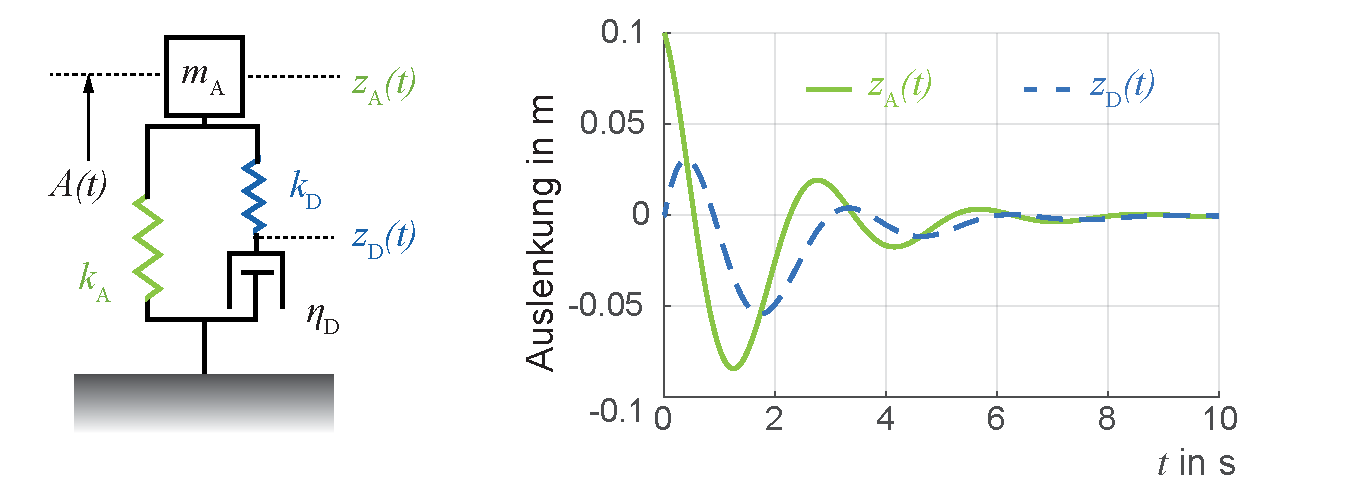
\includegraphics[width=\textwidth]{Stossdaempfer03.pdf}%
\caption[D�mpfung eines Fahrzeuges mit Sto�d�mpfer.]{D�mpfung eines Fahrzeuges mit Sto�d�mpfer f�r typische Parameter: Masse Auto $\SI{2000}{\kilo\gram}$, Federkonstante Auto $\SI{3000}{\N\per\metre}$,  Federkonstante Sto�d�mpfer $\SI{8000}{\N\per\metre}$, D�mpfung Sto�d�mpfer $\SI{5000}{\kg\per\s}$, \vgl \mlbewref{VibDaempfung01.m}} 
\label{abb:bew_Stossdaempfer03}
\end{figure}
			
\newpage
	\subprob{Schwingungstilgung bei Tischen und Deckenaufh�ngungen}

Wir berechnen den Fall der Schwingungsd�mpfung eines an einer Decke h�ngenden Ger�tes (\zb eines Operationsmikroskops)
der Masse $m_\text{G}$, die zur Tilgung angebrachte Gegenmasse sei $m_\text{T}$. Die Lagrange-Funktion lautet
\begin{align}
  \mathcal L=T-U
  &=\frac{m_\text{G}}{2}{\dot{z}_\text{G}}{}^2+\frac {m_\text{T}}{2}{\dot{z}_\text{T}}{}^2 - \frac{k_\text{G}}2\,{z_\text{G}}{}^2 - \frac{k_\text{T}}2\,(z_\text{T}-z_\text{G})^2 \,,
  \label{bew_tilgung01}
\end{align}

woraus sich die Lagrange-Gleichungen bei Ber�cksichtigung von D�mpfung $\eta_\text{G}, \eta_\text{T}$
und einer externen harmonischen Anregung 
\begin{align}
  m_\text{G}\,\ddot{z}_\text{G}+\eta_\text{G}\,\dot{z}_\text{G} + (k_\text{G}+k_\text{T})\,z_\text{G}-k_\text{T}\,z_\text{T} & = k_\text{G}\,A_\text{ext}\,\e^{i\omega t} \notag\\
  m_\text{T}\,\ddot{z}_\text{T}+\eta_\text{T}\,\dot{z}_\text{T} + k_\text{T}\,(z_\text{T}-z_\text{G})        & = 0
  \label{bew_tilgung02}
\end{align}
ergeben. F�r die spezielle inhomogene L�sung\footnote{Wegen der D�mpfung ist nur die spezielle L�sung der inhomogenen
Differentialgleichung\index{Differentialgleichung!inhomogene} relevant.} machen wir den Ansatz
\begin{align}
  z_\text{G} = A_\text{G}\,\e^{\im(\omega t-\varphi_\text{G})}\,,~~~z_\text{T} = A_\text{T}\, \e^{\im(\omega t-\varphi_\text{T})}\,,
  \label{bew_tilgung03}
\end{align}
was auf
\begin{align}
\begin{split}
  A_\text{G}\left[-m_\text{G}\omega^2+\im\,\eta_\text{G}\omega+k_\text{G}+k_\text{T}\right]e^{-i\varphi_\text{G}}
  -A_\text{T}[k_\text{T}]\,\e^{-\im\varphi_\text{T}}
  &=k_\text{G} A_\text{ext} \\
  A_\text{G}[-k_\text{T}]\e^{-\im\varphi_\text{G}}+A_\text{T}\left[-m_\text{T}\omega^2+\im\,\eta_\text{T}\omega+k_\text{T}\right]e^{-\im\varphi_\text{T}}&=0
\end{split}   \label{bew_tilgung04}
\end{align}
f�hrt.
Das ist ein lineares Gleichungssystem in $A_\text{G}$ und $A_\text{T}$. In der zweiten Gleichung von \eqref{bew_tilgung04} sind $A_\text{G}$ und $A_\text{T}$ reell, deshalb gilt:
\begin{align}
\begin{split}
  A_\text{T} = \frac{k_\text{T}}{\sqrt{(k_\text{T}-m_\text{T}\,\omega^2)^2+(\eta_\text{T}\,\Omega)^2}}A_\text{G} ~~~\text{und}\\
	\sqrt{(k_\text{T}-m_\text{T}\,\omega^2)^2+(\eta_\text{T}\,\omega)^2}\,e^{\im\gamma_1}\,\e^{-\im(\varphi_\text{T}-\varphi_\text{G})}A_\text{T}\stackrel!=\textsf{reell}
\end{split}
  \label{bew_tilgung05}
\end{align}
Mit \eqref{bew_tilgung05} haben wir eine Beziehung zwischen den Amplituden
$A_\text{T}$ und $A_\text{G}$ und wir setzen noch:
\begin{equation}
  Q_1= \sqrt{(k_\text{T}-m_\text{T}\,\omega^2)^2+(\eta_\text{T}\,\omega)^2}\,.  \label{bew_tilgung06}
\end{equation}
Das Argument $\gamma_1$ ist gegeben durch
\begin{align}
  \gamma_1=\arctan\frac{\eta_\text{T}\,\omega}{k_\text{T}-m_\text{T}\,\omega^2}+\underbrace\pi_{%
  \text{f�r }m_\text{T}\omega^2 > k_\text{T}} ~~\text{mit}~~ \varphi_\text{T} = \varphi_\text{G} + \gamma_1\,.
  \label{bew_tilgung07}
\end{align}
\newpage
Wir setzen \eqref{bew_tilgung05} und \eqref{bew_tilgung06} in die erste Gleichung von
\eqref{bew_tilgung04} ein und erhalten nach etwas algebraischer
Umformung eine Beziehung zwischen $A_\text{G}$ und $A_\text{ext}$:

\begin{align}
  \underbrace{%
  \left[Q_2\,\e^{\im\gamma_2}-\frac{k_\text{T}^2}{Q_1}\,\e^{-\im\gamma_1}\right]A_\text{G}}_{T_1}
  = \underbrace{k_\text{G}\,A_\text{ext}}_{T_2}\,\e^{\im\varphi_\text{G}}\,,\label{bew_tilgung08}
\end{align}
worin
\begin{align}
  Q_2 &= \sqrt{(k_\text{G}+k_\text{T}-m_\text{G}\,\omega^2)^2+(\eta_\text{G}\,\omega)^2}\,,\\
  \gamma_2 &= \arctan\frac{\eta_\text{G}\,\omega}{k_\text{G}+k_\text{T}-m_\text{G}\,\omega^2}
  +\underbrace\pi_{\text{f�r }m_\text{G}\omega^2>k_\text{G}+k_\text{T}}   \label{bew_tilgung08a}
\end{align}
ist. Aus der Forderung, dass in \eqref{bew_tilgung08} $\left|T_1\right|=T_2$ sein muss, folgt dann das endg�ltige Ergebnis
f�r die Amplitude der Masse $m_\text{G}$ in Abh�ngigkeit von der Anregungsfrequenz und der Anregungsamplitude:
\begin{align}
  A_\text{G} = \frac{k_\text{G}\,A_\text{ext}}{\sqrt{(k_\text{T}{}^2/Q_1)^2+Q_2^2-2(k_\text{T}{}^2/Q_1)Q_2\cos(\gamma_1+\gamma_2)}}\,.
  \label{bew_tilgung09}
\end{align}

\begin{figure}[H]\centering
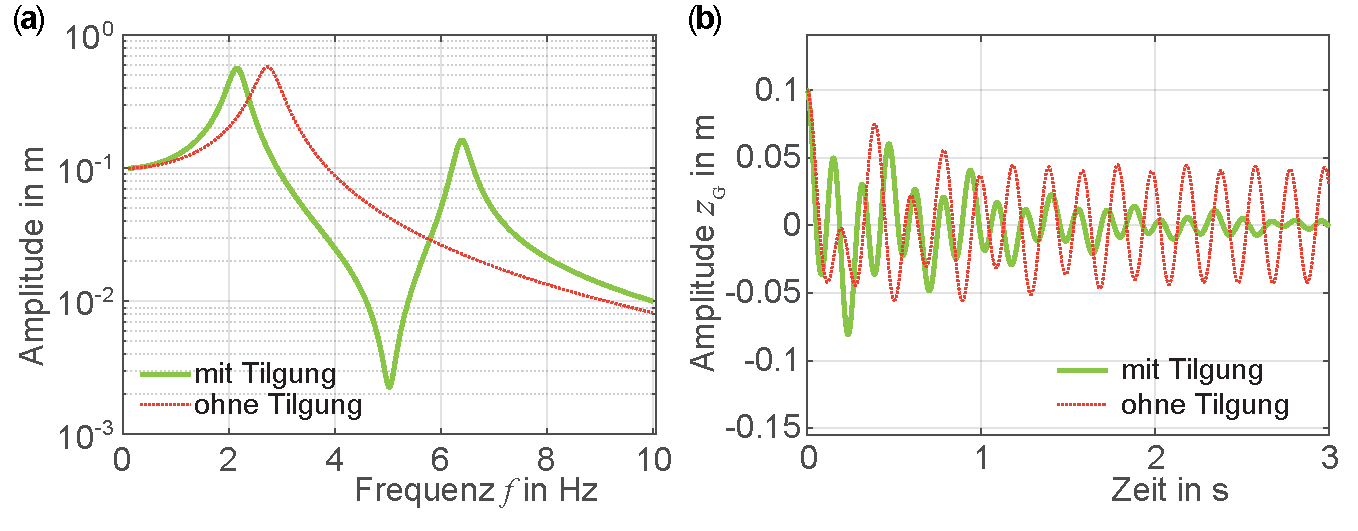
\includegraphics[width=\textwidth]{Tilgung04.pdf}%
\caption[Frequenzgang bei der Schwingungstilgung]{\fa Frequenzgang bei der Schwingungstilgung. Parameter: Masse Mikroskop $m_\text{G} =\SI{50.0}{\kg}$, 
Gegenmasse $m_\text{T} =\SI{25.0}{\kg}$, Federkonstante $k_\text{G} =\SI{15000.0}{\N\per\metre}$, Federkonstante $k_\text{T} =\SI{25000.0}{\N\per\metre}$, D�mpfung Ger�t $\eta_\text{G} =\SI{150.0}{\kg\per\s}$, D�mpfung Gegenmasse $\eta_\text{T}=\SI{100.0}{\kg\per\s}$, Eigenfrequenz Ger�t $f_\text{G}=\SI{2.76}{\per\s}$. Eigenfrequenz Gegenmasse $f_\text{T}=\SI{5.03}{\per\s}$. Man sieht, dass in dem gew�hlten Fall St�rfrequenzen bei 5 Hz optimal unterdr�ckt werden. Gleichzeitig treten aber bei $f \approx \SI{2.2}{\per\s}$ und $f \approx \SI{6.5}{\per\s}$ erhebliche Schwingungsverst�rkungen auf. \fb Einschwingverhalten der Schwingungstilgung bei den gew�hlten Parametern, \vgl \mlbewref{VibDaempfung02.m}}
\label{abb:bew_Tilgung03}
\end{figure}

In \figref{bew_Tilgung03}\,a sind die Amplitudeng�nge f�r die schwingenden
Massen $m_\text{G}$, $m_\text{G}$ nach \eqref{bew_tilgung09} und \eqref{bew_tilgung05}
dargestellt und zum Vergleich die Resonanzkurve einer Masse $m_\text{G}$,
die nur einer Federung mit der Konstanten $k_\text{G}$ unterliegt.
Man sieht sehr sch�n, dass durch die Schwingungstilgung mit der Masse $m_\text{T}$
die Amplitude der Masse $m_\text{G}$ in der Umgebung der Frequenz
$\omega_{0,T}=\sqrt{k_\text{T}/m_\text{T}-\text{T}}$ wirkungsvoll ged�mpft wird.\footnote{%
Man sieht aus \figref{bew_Tilgung03}\,a, dass es in benachbarten Frequenzbereichen durchaus
zu Verst�rkungen kommen kann. So wird zwar bei \SI{5}{\hertz} eine optimale D�mpfung erreicht, aber schon bei \SI{4}{\hertz} \bzw \SI{6}{\hertz} k�nnen gr��ere Auslenkungen beobachtet werden.} In \figref{bew_Tilgung03}\,b haben wir das Einschwingverhalten von $z_\text{G}(t)$ f�r eine Anregung bei \SI{5}{\hertz} mit und ohne Tilgung dargestellt.

	\subprob{Schwingungstilgung bei Hochh�usern}

\begin{figure}[H]\centering
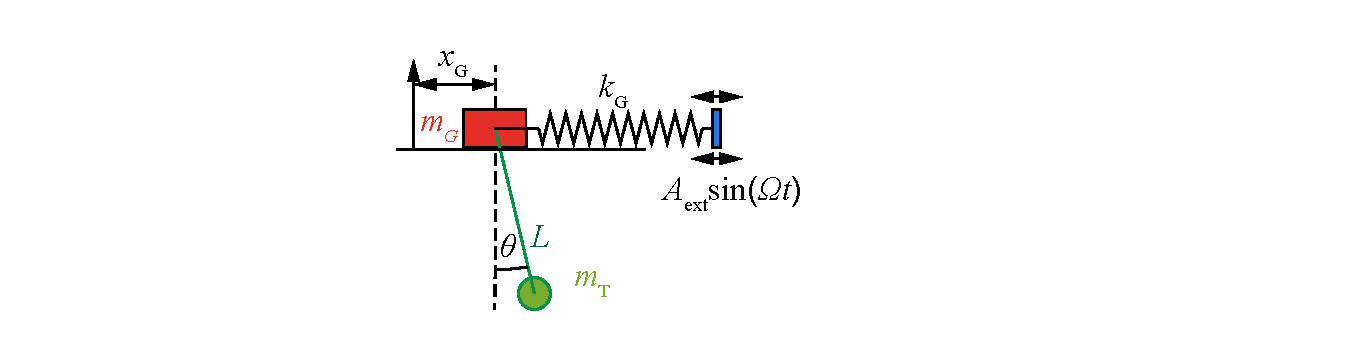
\includegraphics[width=\textwidth]{Tilgung03.pdf}%
\caption[Prinzip des Gleitpendels und entsprechende Schwingungstilgung]{Prinzip des Gleitpendels. Hierin ist $m_\text{G}$ die effektiver Masse des Geb�udes, $m_\text{T}$ die Masse des Gegengewichts (Pendel), $L$ die Pendell�nge und $A_\text{ext}$ die externe Anregung. $k_\text{G}$ ist eine fiktive Federkonstante, die sich empirisch aus der Eigenfrequenz und der Masse des Hochhauses berechnen l�sst. F�r die Schwingungsperiode in Hochh�usern gilt folgende empirische N�herungsformel: $T ~\lek \text{in}~\SI{}{\second} \rek \approx H/46 \lek ~H~~\text{in}~\SI{}{\metre} \rek$.\\
F�r eine Prinziprechnung f�r die Dynamik des Gleitpendels wurde folgende exemplarische Parameter angenommen: $m_\text{G} =\SI{1.0}{\kg}$, $m_\text{T} =\SI{0.3}{\kg}$, $k_\text{G} =\SI{10.0}{\N\per\metre}$, L�nge Pendel $L =\SI{1.0}{\metre}$, D�mpfung Masse $\eta_\text{G} =\SI{0.6}{\kg\per\s}$, D�mpfung Gegenmasse $\eta_\text{T} =\SI{0.2}{\kg\per\s}$, Anregungskreisfrequenz $\omega =\SI{3.13}{\per\s}$, Anregungsamplitude $A_\text{ext} = \SI{0.10}{\metre}$, \vgl \mlbewref{Tilgung01.m}, \mlbewref{Tilgung02.m} und \mlbewref{Tilgung03.m}}
\label{abb:bew_Tilgung04}
\end{figure}

F�r Tilgung von Schwingungen in Hochh�usern gibt es zahlreiche Ausf�hrungsformen, die in vielen F�llen auf zwei mechanische Grundformen zur�ckgef�hrt werden k�nnen: 
\begin{enumerate}[a)]
  \item Ged�mpftes Pendel nach \figref{bew_Tilgung01}
  \item Gleitpendel nach \figref{bew_Tilgung04}\,a
\end{enumerate}

Wir k�nnten das Problem nach dem in Kap.~\ref{kap:bew_Tilgung} beschriebenen Verfahren l�sen, wollen hier aber das spezifische Problem der Gleitpendel-Ausf�hrung detaillierter betrachten. Wir �berlassen dem Leser den Fall a) nach \figref{bew_Tilgung01}. F�r das Gleitpendel k�nnen wir aus \figref{bew_Tilgung04}\,a die folgende Lagrange-Funktion bestimmen:
\begin{align}
  \mathcal{L}
  &=\underbrace{\frac {m_\text{G}}{2}\dot x^2+\frac {m_\text{T}}{2}\left(\dot x_\text{G}^2+L^2\dot\varphi^2+2L\dot\varphi\dot x_\text{G}\cos\varphi\right)}_{T} + \ldots \nonumber \\
	 &~~ - \underbrace{\lk m\,g\,L\,(1-\cos\varphi)+\frac {k_\text{G}}{2}\left(x_\text{G}-A_\text{ext}\sin(\omega t)\right)^2\rk}_{U}
  \label{bew_tilgung10}
\end{align}
Die Dissipationsfunktion $U_\text{R}$ (\vgl \kap{bew_Lagrange_II_R}) ist gegeben durch:
\begin{align}
  U_\text{R} = \frac{\eta_\text{G}}2\dot x_\text{G}^2+\frac{\eta_\text{T}}2\left(\dot x_\text{G}^2+L^2\dot\varphi^2+2L\dot\varphi\dot x_\text{G}\cos\varphi\right)\,.
  \label{bew_tilgung11}
\end{align}

Die Lagrange-Gleichungen berechnen sich dann zu:\\

\begin{align}
\begin{split}
    (m_\text{G}+m_\text{T})\ddot{x} &= -\lbrack k_\text{G}\,x + m_\text{T}\,L\,\ddot{\varphi}\,\cos\varphi - m_\text{T}\,L\,\dot{\varphi}^2\,\sin\varphi - \eta_\text{G}\,\dot{x} - \eta_\text{T}\, \lk \dot{x} + L\,\dot{\varphi}\,\cos\varphi \rk \rbrack \\ & \quad  ~~ + k_\text{G}\,A_\text{ext}\,\sin(\omega t)  \\  \label{eq:bew_GleitP01}
    m_\text{T}\,L\,\ddot{\varphi} &= -m_\text{T}\,\lek \ddot{x}\,\cos\varphi + g\,\sin\varphi\rek - \eta_\text{T}\,\lk \dot{x}_{\cos\varphi} + L\,\dot{\varphi}\rk \;.
\end{split} 
\end{align}
Wir k�nnen f�r kleine $\varphi$, $x$ die beiden Gleichungen linearisieren und setzen die zweite in die erste ein, womit wir erhalten:
\begin{align}
\begin{split}
    \ddot{x} &= -\frac{1}{m_\text{G}+m_\text{T}}\,\lek k_\text{G}\,x + m_\text{T}\,L\,\ddot{\varphi} + \eta_\text{G}\,\dot{x} + \eta_\text{T}\lk \dot{x} + L\,\dot{\varphi} \rk - k_\text{G}\,A_\text{ext}\,\sin(\omega t)\rek \\
    m_\text{T}\,L\,\ddot{\varphi} &= -m_\text{T}\,\lek \ddot{x} + g\,\varphi \rek - \eta_\text{T}\,\lk \dot{x} + L\,\dot{\varphi}\rk \,.
  \end{split} \label{eq:bew_GleitP03}
\end{align}
Wir erhalten dann f�r $\ddot{x}$ und $\ddot{\varphi}$
\begin{align}
\begin{split}
  \ddot{x} &= -\frac{1}{m_\text{G}}\,\lek k_\text{G}\,x -m_\text{T}\,g\,\varphi + \eta_\text{G}\,\dot{x} - k_\text{G}\,A_\text{ext}\,\sin(\omega t)\rek \, \\
  \ddot{\varphi} = &+\frac{1}{m_\text{G}\,L}\,\lek k_\text{G}\,x m_\text{T}\,g\,\varphi + \eta_\text{G}\,\dot{x}  - k_\text{G}\,A_\text{ext}\,\sin(\omega t)\rek - \lek \frac{\eta_\text{T}}{m_\text{T}\,L}\,\lk \dot{x} +L\,\dot{\varphi}\rk + \frac{g}{L}\,\varphi \rek \,.
\end{split} \label{eq:bew_GleitP04}
\end{align}

Die numerische L�sung erfolgt in \mlbewref{Tilgung03.m} und ist in \figref{bew_Tilgung04}b gezeigt. Aus der Abbildung erkennt man sehr sch�n, dass das Pendel die schwingende Masse sehr effektiv d�mpft und dass die Pendelschwingung der Schwingung der Hauptmasse um etwa $\pi/2$ nacheilt. Durch diese Phasenverschiebung zwischen den beiden Schwingungen kommt letztendlich die effektive D�mpfung zustande. Ein Problem bei der gew�hlten Auslegung ist, dass das Pendel relativ stark ausgelenkt wird ($\approx 45\degree$)  und eigentlich unsere lineare N�herung schon nicht mehr gilt. Au�erdem stellt eine solch starke Auslenkung an die Baukonstruktion erhebliche Anforderungen. Wie diese gel�st wurden, kann man sich \zb bei dem Geb�ude $101$ in Taipei oder dem Berliner Fernsehturm ansehen (siehe auch \cite{Ucke2008}).\\ 

Wir haben einige Werte und Absch�tzungen (in rot) aus unserem Modell in der Tabelle \ref{tab:bew_hihrises} zusammengefasst und sind dabei folgenderma�en vorgegangen:
\begin{enumerate}
	\item Annahmen
	\begin{align*}
    \eta_\text{G}= 0\,,~~~~~ \omega_\text{G}{}^2 = \frac{k_\text{G}}{\lk m_\text{G}+m_\text{T}\rk}\,,~~~~~~ \frac{m_\text{T}}{m_\text{G}}=\gamma\,,~~~~~~~~ \eta_\text{G} \neq 0\,,~~~~~~ \omega_\text{T}{}^2=\frac{g}{L}\,.
\end{align*}
\item F�r die L�sung des DGL-Systems \eqref{eq:bew_GleitP03} machen wir folgenden Ansatz:
\begin{align*}
    x &= \hat{X}\,\e^{\im\omega t}\,,~~~~~~~~   \varphi = \hat{\phi}\,\e^{\im\omega t}\,,~~~~~~~~   F = \underbrace{k_\text{G}\,A_\text{ext}}_{\substack{F_x}}\,\e^{\im\omega t}\,,  \\
    \rightarrow ~ \hat{F}_\text{ext} &=  -\omega^2\,\hat{X} + \frac{k_\text{G}}{m_\text{G}+m_\text{T}}\,\hat{X} + \frac{m_\text{T}}{m_\text{G}+m_\text{T}}\,L\,\hat{\phi}\,\lk -\omega^2\rk + \im\omega\frac{\eta_\text{T}}{m_\text{G}+m_\text{T}}\,\lk \hat{X} + L\,\hat{\phi}\rk \,.
\end{align*}
\item Es ergibt sich folgendes lineares Gleichungssystem: 
\begin{align*}
    \hat{X}\,\underbrace{\lk -\omega^2 + \omega_\text{G}{}^2 + \im\omega\,\frac{\eta_\text{T}}{m_\text{G}+m_\text{T}}\rk}_{A} + \hat{\phi} \underbrace{\lk-\frac{\gamma}{1+\gamma}\,L\,\omega^2 + \im\omega\,\frac{L\,\eta_\text{T}}{m_\text{G}+m_\text{T}}\rk}_{B} &= \ldots \\
		\frac{k_\text{G}\,A_\text{ext}}{m_\text{G}+m_\text{T}} = \omega_\text{G}{}^2\,A_\text{ext} &= \hat{F}_\text{ext}\,,\\
    \hat{X}\,\underbrace{\lk -\frac{\omega^2}{L} + \im\omega\,\frac{\eta_\text{T}}{m_\text{T}\,L}\rk}_{C} + \hat{\phi} \underbrace{\lk  -\omega^2 + \omega_\text{T}{}^2 + \im\omega\,\frac{\eta_\text{T}}{m_\text{T}}\rk}_{D}  &= 0 \,.
\end{align*}
\item Wir l�sen das lineares Gleichungssystem nach $\hat{X}$: 
\begin{align*}
    \hat{X}\,A + \hat{\phi}\,B &= \hat{F}_\text{ext} ~ ~\big| \cdot D \,,~~~~~~ \hat{X}\,C + \hat{\phi}\,D = 0 ~~ \big| \cdot B  \\
    \rightarrow ~~~~ \hat{X}  &= \frac{\hat{F}_x\,D}{AD-BC} 
\end{align*}
mit
\begin{align*}
    A&= -\omega^2 + \omega_\text{G}{}^2 + \frac{\im\omega\,\eta_\text{T}\,\gamma}{m_\text{T}\,\lk 1+\gamma\rk}\,, & C&= -\frac{\gamma}{1+\gamma}\,L\,\omega^2 + \frac{\im\omega\,\gamma}{m_\text{T}\,\lk 1+\gamma\rk}\,L\,\eta_\text{T}\,,\\
    B&= -\frac{\omega^2}{L} + \frac{\im\omega\,\eta_\text{T}}{m_\text{T}}\,\frac{1}{L}\,, & D&= -\omega^2 + \omega^2 + \im\omega\,\frac{\eta_\text{T}}{m_\text{T}}\,.
\end{align*}
\item Die Frequenzantwort $R\lk\omega\rk$ ist dann gegeben durch 
\begin{align*}
    R\lk\omega\rk = \Big| \frac{\hat{X}}{\omega_\text{G}{}^2\,A_\text{ext}}\Big|
\end{align*}
und in {\figref{bew_Tilgung05}} gezeigt.
\end{enumerate}
\begin{table}%tab
\centering
\caption{Vergleich von Schwingungstilgungen am Geb�ude 101 in Taipei und am Berliner Fernsehturm}
\smallskip
\begin{tabular}{L{4.5cm}L{2.2cm}L{1cm}L{1.8cm}L{1.8cm}}
Physikalische Gr��e	&	 Symbol & Einheit & Taipei 101 & Fernsehturm Berlin \\ \\
\noalign{\smallskip}\hline\noalign{\smallskip}
\smallskip
& & \\
Relevante H�he (ohne Antenne)	&$ H $& m & 448 & 210\\
Eigenfrequenz Geb�ude &$ \omega_M $& \SI{}{\per\second} & 0.628 & 1.257\\
Schwingungsperiode Geb�ude &$ T_M$& \SI{}{\second} &12.5 & 5.5 \\
Masse	Pendel &$ m_\text{T}$& kg & \SI{662e3}{}& \SI{1.5e3}{} \\
\textcolor{blue}{Masseverh�ltnis (angenommen)} &$ \gamma $& &\textcolor{red}{0.05} & \textcolor{red}{0.05}\\
L�nge	Pendel &$ L $& m & \SI{42.0}{} & \SI{5}{}\\
Eigenfrequenz Pendel &$ \omega_\text{T} $& \SI{}{\per\second} &0.48 & 0.22\\
\textcolor{blue}{D�mpfung Pendel (berechnet)}&$\eta_\text{T}$ & $ \SI{}{\kg\per\second}$ &\textcolor{red}{$\SI{5.0e3}{}$} & \textcolor{red}{25}\\
\textcolor{blue}{Auslenkung mit Tilgung (berechnet)} & $R(\omega)A_\text{ext}$ & $\SI{}{\metre}$ & \textcolor{red}{1.4} & \textcolor{red}{0.13} \\
\textcolor{blue}{max. Beschleunigung mit Tilgung}& $R(\omega)A_\text{ext}\,\omega_\text{T}{}^2$ & $\SI{}{\metre\per\second\squared}$ & \textcolor{red}{0.33} & \textcolor{red}{0.25}\\ 
\noalign{\smallskip}\hline\noalign{\smallskip} \\
\noalign{(In blau angemommene bzw. berechnete Gr��en.)}\\
\end{tabular}\\ 
\label{tab:bew_hihrises}
\end{table}
\begin{figure}[H]\centering
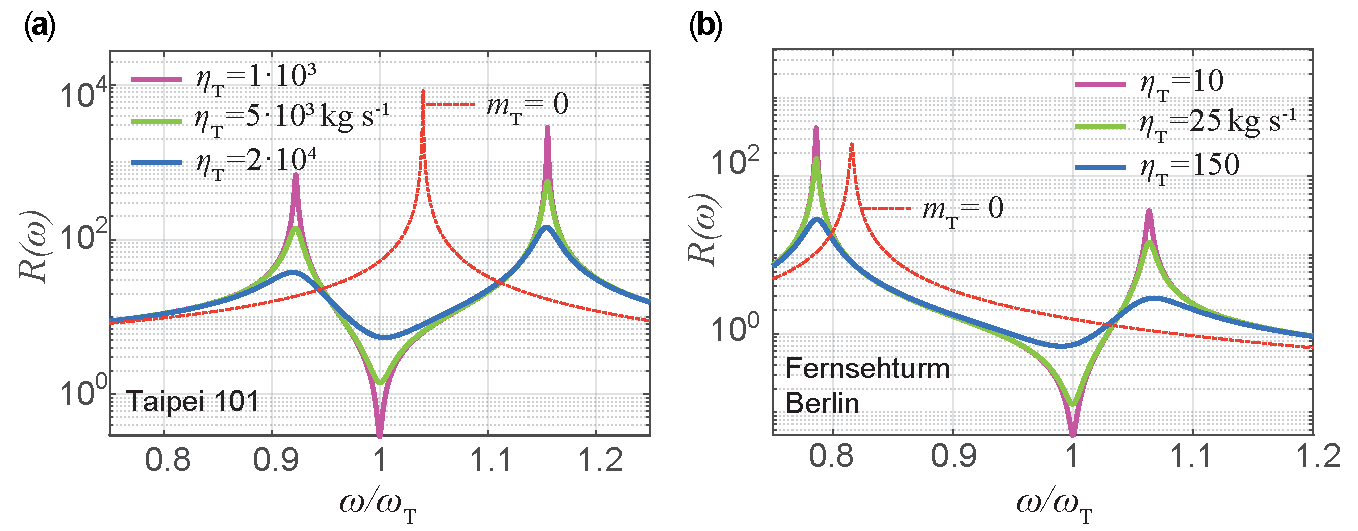
\includegraphics[width=\textwidth]{Tilgung05.pdf}%
\caption[Frequenzantwort des Geb�udes Taipei 101 und des Berliner Fernsehturms]{Modellierung Frequenzantwort des Geb�udes Taipei 101 \fa und des Berliner Fernsehturms \fb . Parameter siehe Tab. \ref{tab:bew_hihrises}} \label{abb:bew_Tilgung05}
\end{figure}

\end{subprobs}
\medskip

\end{sol} 
\textcolor{blue} {$\rightarrow$ zur} \probref{bew_Stossdaempfer}.\\
\noindent\rule[1ex]{\textwidth}{0.5pt}  \newpage

\newpage

\begin{sol}{prob:bew_PendelUeb02}\label{lsg:bew_PendelUeb02} %�bung31
\textbf{Blackwood Pendel, Ballistisches Pendel.} \\ \\
Das Geschoss habe die Geschwindigkeit $v_\text{G}$, die es zu bestimmen gilt und eine Masse $m_\text{G}$, die bekannt ist. Der schwere Holzblock mit der Masse $m_\text{B}$ h�ngt in Ruhe an einer Aufh�ngung der L�nge $L$. \\
Die Maximalauslenkung $\varphi_\text{max}$ wird gemessen. \\
Aus der Energieerhaltung folgt:
\begin{align*}
    U\lk\varphi_\text{max}\rk &= T\lk \varphi=0\rk \\
    \lk m_\text{G}+m_\text{B}\rk\,g\,\Delta z &= \frac{\lk m_\text{G}+m_\text{B}\rk}{2}\,{v_0}^2 \\
\end{align*}
Aus dem Impulssatz folgt:
\begin{align*}
    m_\text{G}\,v_\text{G} &= \lk m_\text{G}+m_\text{B}\rk\,v_0 \\
    v_0 &= \frac{m_\text{G}}{m_\text{G}+m_\text{G}}\,v_\text{G}
\end{align*}
Damit erhalten wir:
\begin{align*}
    g\,L\,\lk 1-\cos\,\varphi_\text{max}\rk &= \frac{1}{2} \lk \frac{m_\text{G}}{m_\text{G}+m_\text{B}}\,v_\text{G}\rk^2 \\
    g\,L\,\lk 1-\cos\varphi_\text{max}\rk &= \frac{{m_\text{G}}}{m_\text{G}+m_\text{B}}\,\frac{{v_\text{G}}^2}{2}
\end{align*}
\begin{align*}
    \rightarrow v_\text{G} = \sqrt{2g\,L\,\lk 1-\cos\varphi_\text{max}\rk}\,\lk 1+\frac{m_\text{B}}{m_\text{G}}\rk
\end{align*}

\end{sol} 
%\href{PhysikUncut_Part1.pdf#prb:bew_PendelUeb02}{\textcolor{blue} {$\rightarrow$ zur \probref{bew_PendelUeb02}.}}\\
\textcolor{blue} {$\rightarrow$ zur} \probref{bew_PendelUeb02}.\\
\noindent\rule[1ex]{\textwidth}{0.5pt}  \newpage


%-----------------------------------------------------------------------------------------------------------
\hypertarget{lsg:bew_PendelUeb04}{}
\begin{sol}{prob:bew_PendelUeb04}\label{lsg:bew_PendelUeb04} %�bung32
\textbf{Wilberforce-Pendel.} \\ \\
Wilberforce zeigte bereits 1895, dass eine Feder mit einer verbundenen zylindrischen Masse L�ngs- und Drehschwingungen ausf�hrt und diese gekoppelt sind. Sommerfeld gab als erster eine umfassende theoretische Beschreibung. Seine Herleitung der Bewegungsgleichungen beruhte auf Prinzipien der Differential\-geometrie. In der ausgezeichneten Arbeit \cite{Koepf1990} wird eine detaillierte Herleitung aus elastomechanischen �berlegungen gegeben. Wir werden hier nur das Ergebnis, d.h. die abgeleitete Lagrange-Gleichung verwenden und empfehlen dem interessierten Leser die Herleitung in \cite{Koepf1990} im Kapitel \ref{kap:kontmech_uebungen} nachzuvollziehen.\\
Die zun�chst �berraschende Eigenschaft des Wilberforce-Pendels resultiert aus einer Kopplung der zwei Bewegungen aufgrund der Geometrie der Feder. Wenn sich die Masse auf und ab bewegt, f�hrt jede Abw�rtsbewegung zu einer leichten Abwicklung der Feder, wodurch die Masse ein kleines Drehmoment erf�hrt. Eine Aufw�rtsbewegung der Masse dagegen l�sst die Windungszahl der Feder, d.\,h. die Zahl der Windungen pro L�nge leicht ansteigen und gibt damit der Masse ein kleines Drehmoment in die andere Richtung. Jede Auf- und Abschwingung f�hrt also zu einem Drehmoment und damit wird mit jeder Schwingung Energie von der Vertikalschwingung in die Torsionsschwingung �bertragen, sodass die Amplitude der Torsionsschwingung anw�chst und gleichzeitig die der Vertikalschwingung abnimmt.
Unter der Annahme einer linearen Kopplung zwischen diesen beiden Schwingungen
kann die Lagrange-Funktion geschrieben werden als
\begin{align}
    \mathcal{L} = \frac{1}{2}\,m_\text{F}\,\dot{z}^2 + \frac{1}{2}\,J_\text{T}\,\dot{\varphi}^2 - \frac{1}{2}\,k_\text{F}\,z^2-\frac{1}{2}\,D_\text{T}\,\varphi^2-\frac{1}{2}\,\kappa\,z\,\varphi \,, \label{eq:bew_wilberforce02}
 \end{align}
wobei der Kopplungskoeffizient mit $\kappa$ bezeichnet wurde und die Indizes F \bzw T sich jeweils auf die vertikale Federschwingung \bzw die horizontale Torsionsschwingung beziehen. 
F�gt man nun geschwindigkeitsproportionale Reibung, parametriert durch die Reibungskoeffizienten $\eta_\text{F}$ bzw. $\eta_\text{T}$, hinzu und ersetzt $\omega_\text{F}{}^2 = k_\text{F}/m_\text{F}$ und $\omega_\text{T}{}^2 = D_\text{T}/J_\text{T}$, so erh�lt man 
%Aus \eqref{eq:bew_wilberforce02} folgen dann mit $\omega_\text{F}{}^2 = k_\text{F}/m_\text{F}$ und $\omega_\text{T}{}^2 = D_\text{T}/J_\text{T}$ und den hinzugef�gten Reibungstermen $\eta_\text{F}$ bzw. $\eta_\text{T}$ 
die Bewegungsgleichungen f�r die gekoppelten Oszillatoren des Wilberforce-Pendels:
\begin{align}
    \begin{split}
        \ddot{z}  + {\omega_\text{F}}^2\, z +\frac{1}{2}\frac{\kappa}{m_\text{F}}\,\varphi 
			          	+ \frac{\eta_\text{F}}{m_\text{F}}\,\dot{z} &= 0 \,,\\
        \ddot{\varphi} + {\omega_\text{T}}^2\,\varphi + \frac{1}{2}\frac{\kappa}{J_\text{T}}\, z 
				          + \frac{\eta_\text{T}}{J_\text{T}}\,\dot{\varphi} &= 0\,.
    \end{split} \label{eq:bew_wilberforce03}
\end{align}
Aus \eqref{eq:bew_wilberforce03} kann man (etwas vereinfachend formuliert) ablesen: Die longitudinale Eigenfrequenz der Feder ist durch $\omega_\text{F}=\sqrt(k_\text{F}/m_\text{F})$ gegeben, die Eigenfrequenz der Rotationsschwingung durch $\omega_\text{T}=\sqrt(D_\text{T}/J_\text{T})$. Wenn beide Eigenfrequenzen �bereinstimmen ($\omega_\text{F}\approx\omega_\text{T}$), kommt es zur Resonanz und zum ausgepr�gten "`Hin- und Herschaukeln"' der Energie (\figref{bew_wilberforce02}). Die Resonanzabstimmung kann man mit einer Fein\-abstimmung der Massen auf der Torsionsstange erreichen. Bei gro�er Verstimmung oder auch starker Reibung verschwindet jedoch der Oszillationseffekt der Energie.\\
Wir haben diese Art von gekoppelten DGL bereits in Kapitel \ref{kap:bew_pendulum_coupled} sowohl im Kleinwinkelverhalten, als auch mit der Methode der Normalmoden untersucht. Wir wollen zun�chst aber auf die numerische Behandlung zur Berechnung des zeitlichen Verhaltens des Pendels und der Energie unter L�sung des Gleichungssystem \eqref{eq:bew_wilberforce03} eingehen.
F�r eine folgende numerische Berechnung wollen wir das Gleichungssystem \eqref{eq:bew_wilberforce03} gleich um  einen Antrieb ($A_\text{F}, B_\text{T}, \omega$) und weitere durch Reibungseffekte motivierte nichtlineare Terme ($\epsilon_\text{F}\,\omega_\text{F}{}^2\,z^3$ \bzw $\epsilon_\text{T}\,\omega_\text{T}{}^2\,\varphi^3$) erweitern. 
Wir erhalten dann aus \eqref{eq:bew_wilberforce03}: 
\begin{align}
   \begin{split}
      \ddot{z} + {\omega_\text{F}}^2\,\lk z + \epsilon_\text{F}\,z^3 \rk 
			         + \frac{1}{2}\frac{\kappa}{m_\text{F}}\,\varphi 
			         + \frac{\eta_\text{F}}{m_\text{F}}\,\dot{z}  
							&= A_{\text{F}}\,\sin\omega t\,,  \\
      \ddot{\varphi} + {\omega_\text{T}}^2\, \lk \varphi + \epsilon_\text{T}\,\varphi^3 \rk 
			         + \frac{1}{2}\frac{\kappa}{J_\text{T}}\,z +  \frac{\eta_\text{T}}{J_\text{T}}\,\dot{\varphi} 
							&= B_\text{T}\,\sin\omega t \,.
    \end{split} \label{eq:bew_wilberforce04}
\end{align} 

Wir benutzen f�r die numerischen Rechnungen die Parameter, die ann�hernd dem Wilberforce-Pendel der Fa. Leybold-Didactic entsprechen (Tabelle \ref{tab:bew_wilberforce}) und erhalten die in \figref{bew_wilberforce02} dargestellte zeitliche Dynamik des Schraubenpendels. Man erkennt deutlich das Hin- und Herpendeln der Energie von der Federschwingung auf die Torsionsschwingung.

\begin{figure}[H]\centering
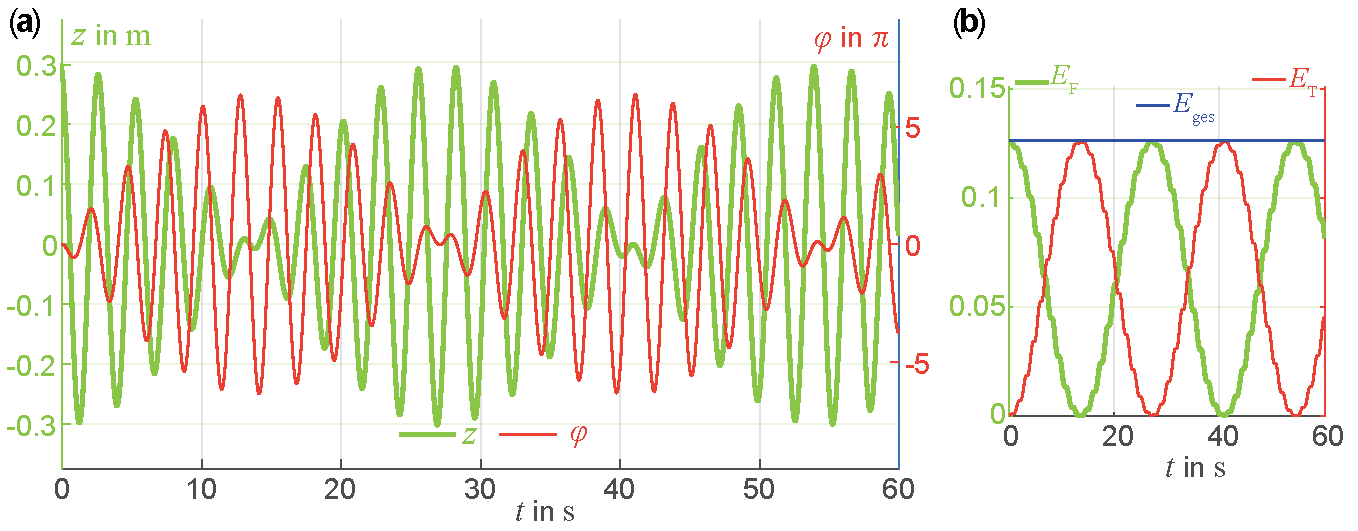
\includegraphics[width=\textwidth]{Wilberforce01.pdf}
\caption[Dynamik des linearen Wilberforce-Pendels (Schwingende Schraubenfeder)]
{Dynamik des linearen Wilberforce-Pendels (Schwingende Schraubenfeder) im Resonanzfall nach \eqref{eq:bew_wilberforce03}. \fa Entwicklung von $z(t)$ und $\varphi(t)$, \fb Energien der Feder $E_\text{F}(t)$ und des Torsionspendels $E_\text{T}(t)$ nach \eqref{eq:bew_wilberforce03}, Parameter siehe Tab. \ref{tab:bew_wilberforce} und  \mlbewref{Wilberforce.m}}
\label{abb:bew_wilberforce02}
\end{figure}

\begin{table}[h!]
\caption{Wesentliche Parameter des Wilberforce-Pendels\cite{Berg1991}}
    \begin{tabular}{L{1.5cm}L{3cm}L{5cm}}
         $m_\text{F}$&$\SI{0.5164}{\kg}$& Masse Federpendel  \\
         $k_\text{F}$&$\SI{2.8}{\newton\per\metre}$& Federkonstante \\
         $L_\text{F}$&$\SI{1.765}{\metre}$& L�nge Feder \\
			   $\omega_\text{F}$&$\SI{2.3286}{1\per\second}$& Eigenfrequenz Feder \\ \\
         %$R_\text{H}$&$\SI{0.015}{\metre}$& Durchmesser der Helix der Feder \\
         %$n$&$125$&  Windungszahl\\ 
         %$\alpha$&$\atan\lk\frac{L_\text{F}}{2\pi\,R_\text{H}\,n}\rk = \SI{0.149}{\radian}$\:& Anstiegswinkel \\         
				 $m_\text{T}$&$\SI{0.418}{\kg}$&  Masse Torsionsgewicht\\
         $J_\text{T}$&$\SI{1.45e-04}{\kg\metre\squared}$ & Tr�gheitsmoment der Torsionsstange   \\
         $D_\text{T}$&$\SI{7.86e-04}{\newton\metre\per\radian}$ & Torsionsmoment \\
				 $\omega_\text{T}$&$\SI{2.3384}{1\per\second}$& Eigenfrequenz Torsionsstange  \\	\\
         $\kappa $&$ \SI{2.73e-03}{\N\per\radian}$& Kopplungskonstante\\
	       $\epsilon_\text{F} $&$ 0.00 \ldots 0.05$& Nichtlinearit�t Feder \\			
	       $\epsilon_\text{T}$&$ 0.00 \ldots 0.02$&Nichtlinearit�t Torsionsstange	\\		
    \end{tabular} 
\end{table} \label{tab:bew_wilberforce}

Als Erweiterung kann man die zeitliche Entwicklung von $\varphi\lk t\rk$ und $z\lk t\rk$ f�r ein nichtlineares, getriebenes Wilberforce-Pendel mit Nichtlinearit�ten ($\epsilon_\text{F} \neq 0$ \bzw $\epsilon_\text{T} \neq 0$) berechnen, vgl. auch \mlbewref{Wilberforce.m}. Man kann zeigen, dass je nach Gr��e der Nichtlinearit�t 
%$\epsilon_\text{F}$ \bzw $\epsilon_\text{T}$ 
die Frequenzen der Schwebung zwischen Feder und Torsionsstange zu kleineren \bzw gr��eren Werten hin \anf{verschoben} werden. Bei bestimmten Verh�ltnissen kann es sogar zu einer Verdopplung der Schwingungsdauer kommen (\figref{bew_wilberforce03}), einem typischen Ph�nomen nichtlinearer Systeme (siehe Kapitel \ref{kap:bew_chaos}).

\begin{figure}[H]\centering
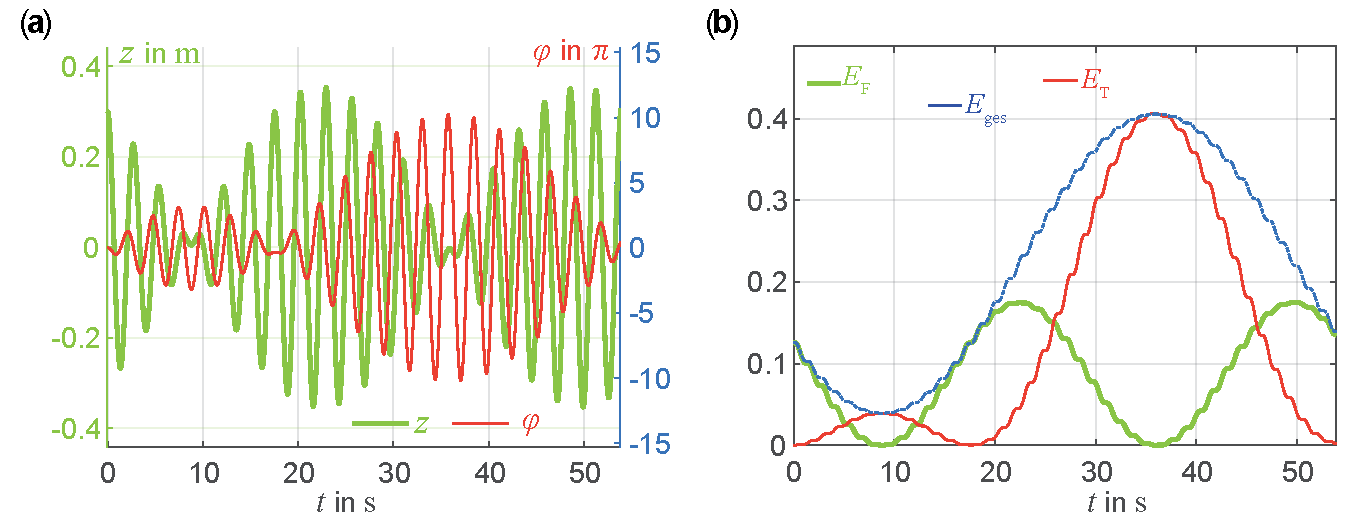
\includegraphics[width=\textwidth]{Wilberforce02.pdf}
\caption[Dynamik f�r das nichtlineare Wilberforce-Pendel .]{Dynamik f�r das nichtlineare Wilberforce-Pendel im Resonanzfall nach \eqref{eq:bew_wilberforce04}. \fa Darstellung von $z(t)$ und $\varphi(t)$ und \fb der Energien von Feder- und Torsionspendel nach \eqref{eq:bew_wilberforce04}, Parameter siehe Tab. \ref{tab:bew_wilberforce} und \mlbewref{Wilberforce.m}, die Reibung wurde vernachl�ssigt und die Nichtlinearit�tskoeffizienten betragen $\epsilon_\text{F}=0.03$ \bzw $\epsilon_\text{T}=0$}\label{abb:bew_wilberforce03}
\end{figure}

Eine Variation des Wilberforce-Pendels ist das Valett-Pendel \cite{Ucke2021}, bei dem sowohl am oberen als auch am unteren Ende der Feder eine Torsionsstange angebracht ist. 
Wir verweisen dazu auf die Referenzen \cite{Koepf1990, Berg1991}, in denen die Aufstellung der Lagrange-Funktion \bzw Lagrange-Gleichungen f�r das Wilberforce-Pendel behandelt wird,  die auf Sommerfeld\indexp{Sommerfeld, Arnold} zur�ck geht. Ganz analog kann man die Differentialgleichungen f�r ein Valett-Pendel aufstellen, wobei wir in diesem Fall drei generalisierte Koordinaten ($z,\, \varphi_1,\, \varphi_2$) haben. Interessant ist, dass bei diesem Pendel, das Auf- und Abwickeln der Feder mit einer jeweils entgegengesetzten Drehung der Torsionstangen am oberen und unteren Ende verbunden ist. Wir verweisen auf  die Zusatzaufgabe in \probref{bew_Zusatz_ValletPendel}.\\

Wir wollen jetzt noch kurz die Vorgehensweise f�r die analytische Berechnung skizzieren und folgen dabei \cite{Berg1991}.\\
Wir starten wieder von \eqref{eq:bew_wilberforce03} (ohne Reibungsterme) und leiten die zweite Gleichung noch zweimal nach der Zeit ab. Wir substituieren $\ddot{z}$ durch die erste Gleichung und erhalten nach einigen Umformungen:
\begin{align}
\frac{\D^4 \varphi}{\D t^4} + \lk \omega_\text{F}{}^2+\omega_\text{T}{}^2 \rk \frac{\D^2 \varphi}{\D t^2}
+ \lk \omega_\text{F}{}^2\omega_\text{T}{}^2 - \frac{\kappa^2}{4\,m_\text{F}\, J_\text{T}}\rk \, \varphi = 0\,.
\label{eq:bew_wilberforce05} 
\end{align} 
Mit dem Ansatz $\varphi(t) = Q\,\e^{\im\omega t}$ findet man die charakteristische Gleichung 
\begin{align}
 \omega^4 - (\omega_\text{F}{}^2 +\omega_\text{T}{}^2) \omega^2 + \lk \omega_\text{F}{}^2\omega_\text{T}{}^2 - \frac{\kappa^2}{4\,m_\text{F}\, J_\text{T}}\rk = 0\,,
\label{eq:bew_wilberforce06}
\end{align}
deren L�sungen lauten:
\begin{align}
 \omega_{1,2}{}^2 &= \frac{1}{2} \lek \omega_\text{F}{}^2 + \omega_\text{T}{}^2 \pm \sqrt{\lk \omega_\text{F}{}^2 - \omega_\text{T}{}^2\rk^2 + \frac{\kappa^2}{\,m_\text{F}\, J_\text{T}}} \rek \,.
\label{eq:bew_wilberforce07}
\end{align} 
F�r den Resonanzfall $\omega_\text{F} = \omega_\text{T} = \omega_0$ ergibt sich:
\begin{align*}
	 \omega_{1,2}{}^2 &= \omega_0{}^2 \pm \frac{1}{2}\sqrt\frac{\kappa^2}{m_\text{F}\, J_\text{T}}\,.
\end{align*}
Wir f�hren die Schwebungsfrequenz
\begin{align}
     \omega_\text{S} = \frac{\kappa}{ 2\omega_0\sqrt{\,m_\text{F}\, J_\text{T}}}\, \label{eq:bew_wilberforce08}
\end{align}
ein und erhalten f�r den Fall, dass $\omega_\text{S} \ll \omega_0$ 
\begin{align}
	 \omega_{1,2} \approx \omega_0 \pm \frac{1}{2}\,\omega_\text{S} = \omega_0 \pm \frac{\kappa}{4\omega_0\sqrt{\,m_\text{F}\, J_\text{T}}} \,. \label{eq:bew_wilberforce08a}
\end{align}

Wir haben damit die Frequenzen $\omega_1$ und $\omega_2$ der beiden Normalmoden hergeleitet. Die Gesamtbewegung des Pendels (\zb des Endpunktes einer Torsionsstange der L�nge $2 l_\text{T}$) kann beschrieben werden durch
\begin{align}
	\vec{X}(t) = z(t)\,\veceZ + l_\text{T}\,\varphi(t)\,\vec{e}_\varphi \,,
  \label{eq:bew_wilberforce09}
\end{align}
worin noch $z(t)$ und $\varphi(t)$ zu bestimmen sind. F�r $\varphi(t)$ und damit $\ddot{\varphi}(t)$ k�nnen wir ansetzen:
\begin{subequations}
\begin{align}
	 \varphi(t) &= A\sin\omega_1 t + B\cos\omega_1 t + C\sin\omega_2 t + D\cos\omega_2 t\,,  \\
	 \ddot{\varphi}(t) &= -\omega_1{}^2\,A\sin\omega_1 t  -\omega_1{}^2\,B\cos\omega_1 t  -\omega_2{}^2\,C\sin\omega_2 t  -\omega_2{}^2\,D\cos\omega_2 t\,.  
\end{align} 	\label{eq:bew_wilberforce10}
\end{subequations}

Wir setzen \eqref{eq:bew_wilberforce10} in \eqref{eq:bew_wilberforce04} ein und erhalten $z(t)$ und auch $\ddot{z}$. Mit den Anfangsbedingungen, $z(0)=z_0\neq 0,\, \varphi(0) = \varphi_0 \neq 0$ und allen  Anfangsgeschwindigkeiten gleich Null sind dann $A, C = 0$ und $B,\, D$ bestimmen sich aus $z_0,\, \varphi_0$\;.
Wir erhalten damit folgenden L�sungen:
\begin{subequations}
\begin{align}
	z(t) &= z_0\,(\omega_1{}^2-\omega_2{}^2)^{-1}\, 
	        \lek (\omega_1{}^2-\omega_\text{T}{}^2)\,\cos\omega_1 t - (\omega_2{}^2-\omega_\text{T}{}^2)                 \,\cos\omega_2 t \rek \nonumber\\
					&- \frac{2J_\text{T}\varphi_0}{\kappa}\,(\omega_1{}^2-\omega_2{}^2)^{-1} \,  
					      (\omega_1{}^2-\omega_\text{T}{}^2)\,  (\omega_2{}^2-\omega_\text{T}{}^2)\,
								(\cos\omega_1 t - \cos\omega_2 t)\,.\\
\varphi(t) &= \frac{\kappa\,z_0}{2J_\text{T}}\,(\omega_1{}^2-\omega_2{}^2)^{-1}\,
                                               (\cos\omega_1 t - \cos\omega_2 t)\,\nonumber \\
	       & + \varphi_0 \,(\omega_1{}^2-\omega_2{}^2)^{-1} 
					   \lek (\omega_1{}^2-\omega_\text{T}{}^2)\,\cos\omega_2 t - (\omega_2{}^2-\omega_\text{T}{}^2)                 \,\cos\omega_1 t \rek \,.
\end{align}   \label{eq:bew_wilberforce11}
\end{subequations}

Damit k�nnen jetzt die Normalkoordinaten bestimmen (\vgl \kap{bew_pendulum_coupled}):
\begin{align}
	\vec{X}(t) &= z(t)\,\veceZ + l_\text{T}\,\varphi(t)\,\vec{e}_\varphi \nonumber \\
	           &= N_\text{n, 1} \cos\omega_1 t\, \vec{n}_1 + N_\text{n, 2} \cos\omega_2 t\, \vec{n}_1\,,
  \label{eq:bew_wilberforce12}
\end{align}
worin die $\vec{n}_i$ die Normalvektoren und die $N_\text{n, i}$ ihre Amplituden sind. 
Man bestimmt leicht
\begin{subequations}
\begin{align}
	\vec{n}_1 &= l_\text{T}\,\vec{e}_\varphi + \frac{2J_\text{T}}{\kappa}\,(\omega_1{}^2-\omega_\text{T}{}^2)\,\veceZ \,\\
	\vec{n}_2 &= l_\text{T}\,\vec{e}_\varphi + \frac{2J_\text{T}}{\kappa}\,(\omega_2{}^2-\omega_\text{T}{}^2)\,\veceZ \,\\
  N_\text{n, 1} &= +(\omega_1{}^2-\omega_2{}^2)^{-1}\,\lek \frac{\kappa\,z_0}{2J_\text{T}} 
	                  - (\omega_2{}^2-\omega_\text{T}{}^2)\,\varphi_0 \rek \,\\
  N_\text{n, 2} &= -(\omega_1{}^2-\omega_2{}^2)^{-1}\,\lek \frac{\kappa\,z_0}{2J_\text{T}} 
	                  - (\omega_2{}^2-\omega_\text{T}{}^2)\,\varphi_0 \rek \,,
\end{align} \label{eq:bew_wilberforce13}
\end{subequations}

wobei wir $l_\text{T}$ eingef�gt haben, damit die Normalenvektoren die Dimension L�nge haben. Will man nur eine der Normalmoden anregen, \zb die mit Frequenz $\omega_1$, dann muss $N_\text{n, 2}=0$ sein, woraus folgt 
	\[z_0=\sqrt{\frac{J_\text{T}}{m_F}}\, \varphi_0\,,
\]
also eine Bedingung f�r die Anfangswerte $z_0,\, \varphi_0$. Wir verweisen auf das \mscr{} \mlbewref{Wilberforce.m}.

\begin{figure}[H]\centering
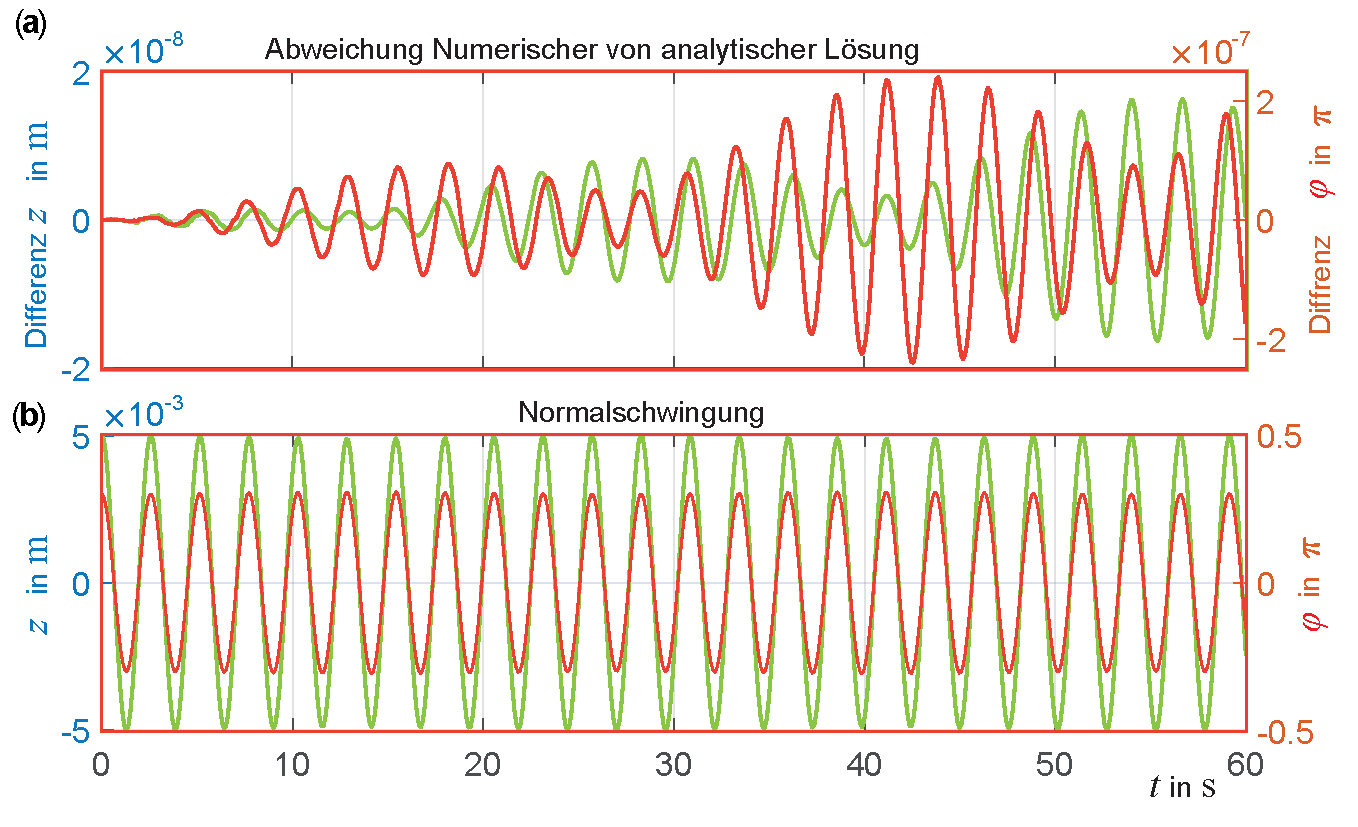
\includegraphics[width=\textwidth]{Wilberforce03.pdf}
\caption[Dynamik des linearen Wilberforce-Pendels nach analytischer und numerischer Rechnung]
{Dynamik des linearen Wilberforce-Pendels nach analytischer und numerischer Rechnung im Resonanzfall nach  \eqref{eq:bew_wilberforce11}. \fa Vergleich der zeitlichen Entwicklung von $z(t)$ und $\varphi(t)$ nach analytischer und numerischer Rechnung nach \eqref{eq:bew_wilberforce11}. \fb Entstehende Normalschwingung $\omega_1$ nach \eqref{eq:bew_wilberforce13} bei der Anfangsbedingung $z_0 = \SI{0.005}{\metre},\, \varphi_0 = \sqrt{m_F/J_\text{T}} = \SI{0.3}{}\pi$, weitere Parameter siehe Tab. \ref{tab:bew_wilberforce} und \mlbewref{Wilberforce.m}}
\label{abb:bew_wilberforce04}
\end{figure}

\end{sol} 
%\href{PhysikUncut_Part1.pdf#prb:bew_PendelUeb04}{\textcolor{blue} {$\rightarrow$ zur \probref{bew_PendelUeb04}.}}\\
\textcolor{blue} {$\rightarrow$ zur} \probref{bew_PendelUeb04}.\\
\noindent\rule[1ex]{\textwidth}{0.5pt}  \newpage

%-----------------------------------------------------------------------------------------------------------

%%%-----------------------------------------------------------------------------------------------------------
%%%-----------------------------------------------------------------------------------------------------------


\subsection{�bungen zu nichtlinearen und komplexen Systemen}
\medskip

%-----------------------------------------------------------------------------------------------------------
\hypertarget{lsg:bew_logisticmap}{}
\begin{sol}{prob:bew_logisticmap}\label{lsg:bew_logisticmap} %�bung33
\textbf{Logistische Gleichung -- Populationsproblem.}\\ \\
Die Berechnungen sind in den \mscren\mlbewref{LogistischeGleichung01.m} und \mlbewref{LogistischeGleichung02.m} ausgef�hrt und in den \figref{bew_logisticmap01} und \figref{bew_logisticmap02} gezeigt.
Man erkennt folgende Charakteristika:

\begin{figure}[H]\centering
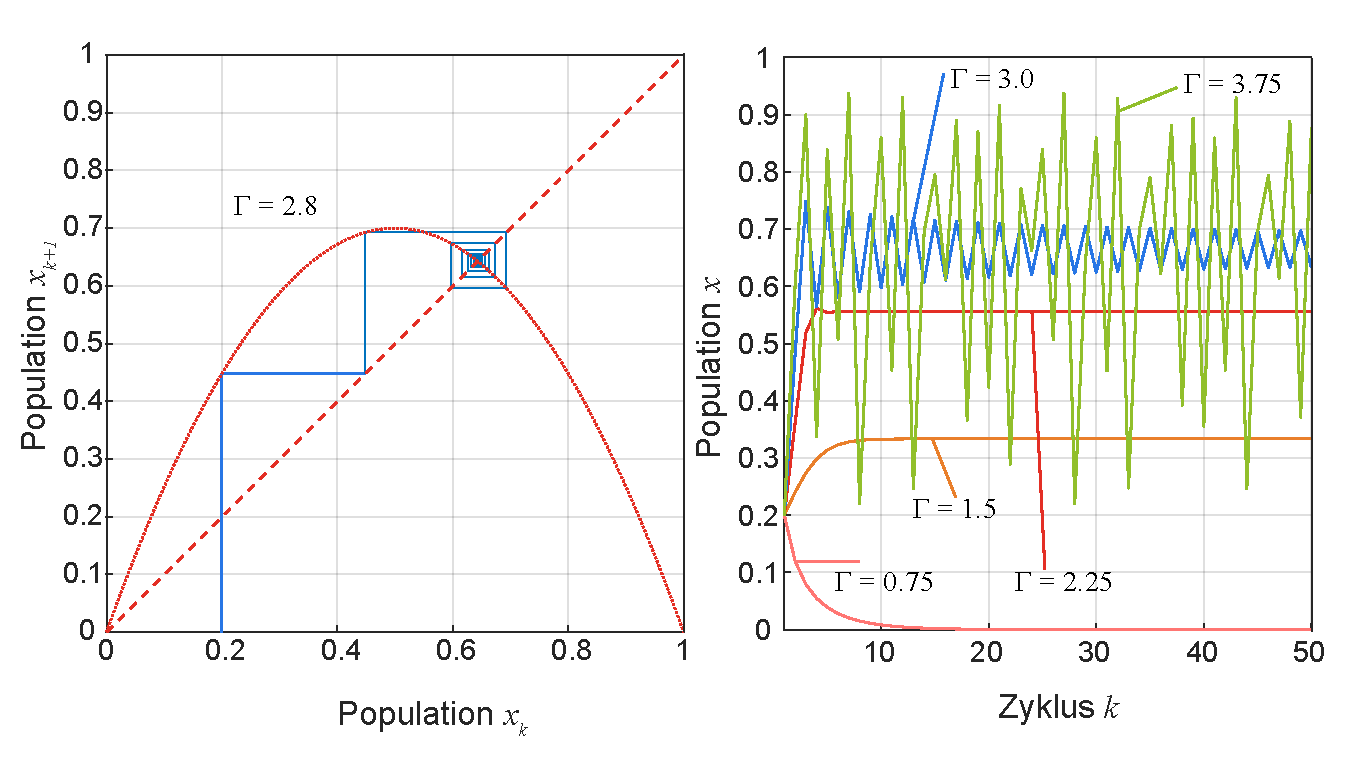
\includegraphics[width=\textwidth]{LogisticMap01.pdf}
\caption[Entwicklung der Populationen nach der Logistischen Gleichung]{Entwicklung der Populationen nach der Logistischen Gleichung f�r verschiedene Gr��en des Wachstumsparameters $\Gamma$}
\label{abb:bew_logisticmap01}
\end{figure}

Bei verschiedenen $\Gamma$ k�nnen wir folgende Verhaltensweisen f�r $k\rightarrow\infty$ beobachten.
Das Verhalten h�ngt nicht vom Anfangswert $x_1$ ab, sondern nur von $\Gamma$:
\begin{enumerate} [a)]
\item $0 < \Gamma < 1$ : Die Population stirbt aus.
\item $1 < \Gamma < 2$ : Die Population n�hert sich monoton dem Grenzwert $\frac {\Gamma-1}{\Gamma}$ an.
\item $2 < \Gamma < 3$ : Die Population n�hert sich dem Grenzwert $\frac {\Gamma-1}{\Gamma}$ alternierend an.
\item $3 < \Gamma < 3.45$ : Die Population wechselt bei fast allen Startwerten zwischen zwei H�ufungspunkten (Bifurkation).
\item $\Gamma >  3.54$ : Es stellen sich immer mehr H�ufungspunkte der Population ein, die Bifurkationsintervalle werden immer kleiner.
\item $\Gamma >  3.57$ : Es beginnt das Chaos.
  Mit weiter wachsendem $\Gamma$ verschmelzen die Bifurkationsintervalle und winzige �nderungen des Anfangswertes resultieren in v�llig unterschiedliche Populationsentwicklungen.
  Dazwischen gibt es aber f�r bestimmte $\Gamma$-Werte wieder H�ufungspunkte, beispielsweise in der N�he von $\Gamma=3.82$. 
\item $\Gamma > 4$ Die Populationsfolge divergiert f�r fast alle Anfangswerte $x_1$ und verl�sst das Intervall {$[0\,1]$}.
\end{enumerate}

\begin{figure}[H]\centering
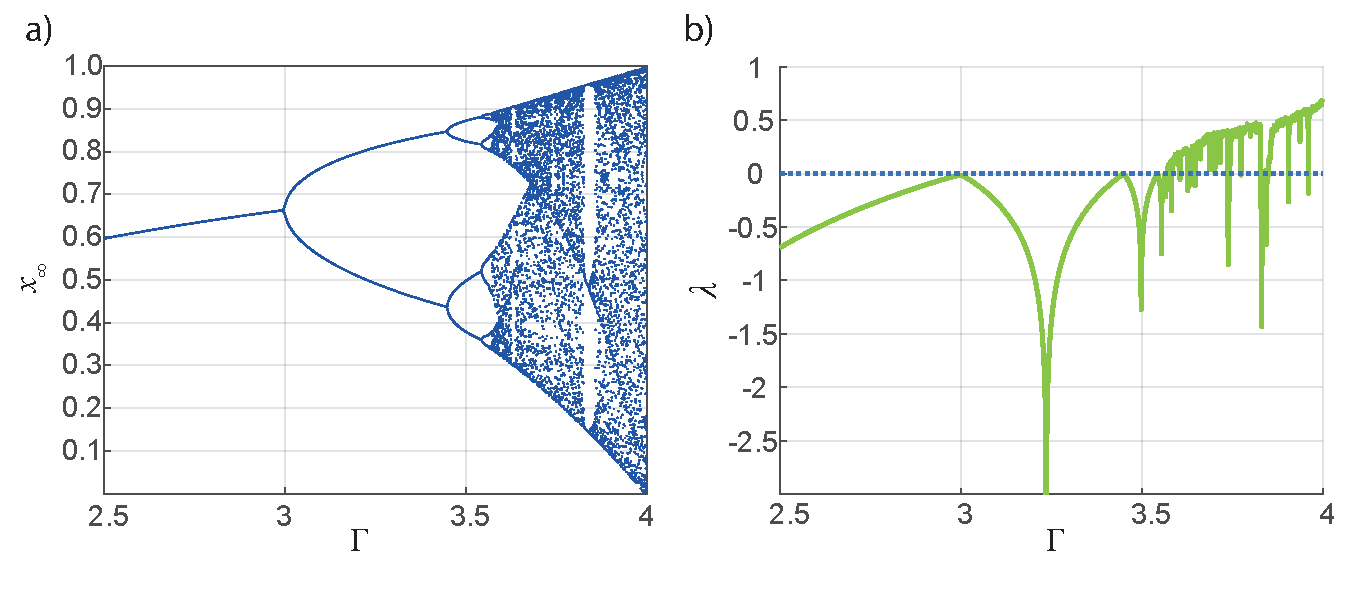
\includegraphics[width=\textwidth]{LogisticMap02.pdf}
\caption[Bifurkationsgraph und Ljapunow-Exponent der Logistischen Gleichung]{Bifurkationsgraph (a) und Ljapunow-Exponent (b) der logistischen Gleichung}\label{abb:bew_logisticmap02}
\end{figure}

Wir wollen jetzt noch zeigen, wie man den Ljapunow-Exponenten berechnen kann.
Es gilt nach \eqref{eq:bew_Chaos01}
    \begin{align*}
        \Delta_0 &= x_0 + \delta - x_0 = \delta \,, \\
        \Delta_1 &= f\lk x_0+\delta\rk -f\lk x_0\rk \approx \delta \frac{\D f}{\D x}\bigg|_{x_0} \,.
    \end{align*}
In unserem Fall ist mit $x_{n+1}=\Gamma\,x_n\,(1-x_n)$ ist $f(x)$ gegegben durch
    \begin{align*}
        f\lk x\rk = \Gamma\,x\lk 1-x\rk \,.
    \end{align*}
F�r die n�chsten Iterationen gilt dann 
    \begin{align}
        \Delta_2 &= f\lk f\lk x_0+\delta\rk-f\lk x_0\rk\rk -f\lk f\lk x_0\rk\rk = f^{\lek 2\rek}\lk x_0+\delta\rk - f^{\lek 2\rek} \lk x_0\rk \,, \nonumber\\
				\Delta_\text{k} &= \ldots \,, ~~ k= 3 \ldots n \,,\nonumber\\
        \Delta_\text{n} &= f^{\lek n \rek} \lk x_0+\delta\rk - f^{\lek n \rek}\lk x_0 \rk \,, \label{eq:bew_Chaos03}
    \end{align}
wobei $f^{\lek n\rek}$ die n-te \glqq Verschachtelung\grqq{} der Funktion $f\lk x\rk$ ist. \\
Mit der Definition des Ljapunow-Exponenten \eqref{eq:bew_Chaos02} wird \eqref{eq:bew_Chaos03} zu
    \begin{align*}
        \Delta_\text{n} = f^{\lek n\rek}\lk x_0+\delta \rk -f^{\lek n\rek}\lk x_0 \rk = \delta\,e^{n\,\lambda} \,,
    \end{align*}
und aufgel�st nach $\lambda$
    \begin{align}
        \lambda = \frac{1}{n}\,ln\,\lek\frac{f^{\lek n\rek}\lk x_0+\delta\rk-f^{\lek n\rek}\lk x_0 \rk}{\delta}\rek\approx \frac{1}{2}\,\ln\,\frac{\D f^{\lek n\rek}}{\D x}\bigg|_{x_0} \label{eq:bew_Chaos04} \,.
    \end{align}
Wie bestimmen wir nun die Ableitung auf der rechten Seite?
Wir wenden dazu die Kettenregel an:
    \begin{align*}
        \frac{\D f^{\lek n\rek}}{\D x}\bigg|_{x_0} = \frac{\D f}{\D x}\bigg|_{x_{\text{n}-1}}\,\frac{\D f}{\D x}\bigg|_{x_{\text{n}-2}}\,\cdots\,\frac{\D f}{\D x}\bigg|_{x_0} \,.
    \end{align*}

\newpage
Im Grenz�bergang $n \rightarrow \infty$ folgt daraus:
    \begin{align}
        \lambda &= \lim_{n\to\infty}\,\frac{1}{n}\,\ln\,\lek  \prod_{k=0}^{n-1}\,\frac{\D f}{\D x}\bigg|_{x_\text{k}}\rek = \lim_{n\to\infty}\,\frac{1}{n}\,\sum_{k=0}^{n-1}\,\frac{\D f\lk x_\text{k}\rk}{\D x} = \lim_{n\to\infty}\,\frac{1}{n}\, \sum_{k=0}^{n-1}\,f'\lk x_\text{k}\rk \,. \label{eq:bew_Chaos05}
    \end{align}
In unserem Fall der logistischen Gleichung ist $f' = \Gamma \,\lk 1-2x\rk$, also
    \begin{align}
        \lambda = \Gamma \,\lim_{n\to\infty}\,\frac{1}{n}\,\sum_{k=0}^{n-1}\,\lk 1-2x_\text{k}\rk \,. \label{eq:bew_Chaos06}
    \end{align}
Auf dieser Basis wurde der Ljapunow-Exponent in \figref{bew_logisticmap02} b) berechnet.

\end{sol} 

%\href{PhysikUncut_Part1.pdf#prb:bew_logisticmap}{\textcolor{blue} {$\rightarrow$ zur \probref{bew_logisticmap}.}}\\
\textcolor{blue} {$\rightarrow$ zur} \probref{bew_logisticmap}.\\
\noindent\rule[1ex]{\textwidth}{0.5pt}  \newpage

%-----------------------------------------------------------------------------------------------------------

\hypertarget{lsg:bew_PendelUeb01}{}
\begin{sol}{prob:bew_PendelUeb01}\label{lsg:bew_PendelUeb01} %�bung34
\textbf{Intrinsisch nichtlineare Oszillatoren.} \\ \\
Man k�nnte vermuten, dass jedes schwingende System bei kleinen Auslenkungen als harmonischer Oszillator angen�hert werden k�nnte. Das ist aber nicht der Fall. Wir wollen zeigen, dass es F�lle gibt, in denen eine Oszillation intrinsisch, \dh auch bei kleinsten Auslenkungen, nichtlinear ist.\\
Nach \eqref{eq:bew_Schwingung_a} bedeutet dies, dass das \pot{} $U\lk q\rk$ in der Taylorentwicklung folgende Struktur haben muss\footnote{Wir beschr�nken uns der Einfachheit halber auf den eindimensionalen Fall.}:
    \begin{align}
        U\lk q\rk = \frac{1}{3!}\,\frac{\d^3U}{\d q^3}\Bigg|_{q=q_0}\lk q-q_0\rk^3+\frac{1}{4!}\,\frac{\d^4U}{\d q^4}\Bigg|_{q=q_0}\lk q-q_0\rk^4+\cdots \,. \label{eq:bew_NLOUe01}
    \end{align}
Hierin ist $q_0$ wieder die Gleichgewichtslage und in \eqref{eq:bew_NLOUe01} verschwindet gegen�ber \eqref{eq:bew_Schwingung_a} der quadratische Term der Taylorentwicklung \index{Taylorentwicklung} \index{Taylorreihe}. \\
Wir k�nnen die Bewegungsgleichungen f�r Beispiele solcher \pot{}e aufstellen und auch numerisch mit \matlab{} l�sen, wollen uns aber zuvor �berlegen, wie eine allgemeinere Formel f�r die Schwingungsdauer eines Oszillators f�r ein \pot{} abgeleitet werden kann, dessen erster nicht verschwindender Term der Taylorentwicklung proportional zu $\d^n U/\dq^n = U^{\lk n\rk}\lk q_0\rk\lk q-q_0\rk^n$ mit $n >1$ ist. Wir setzen \obda $q_0=0$ und starten von Gleichung \eqref{eq:bew_Schwingung_a} mit $U^{(n)}\lk 0 \rk = C$,  die f�r die Amplitude $q_\text{max} = C\,q^n = E$ dann
        \begin{align}
            T = 4\,\sqrt{\frac{m}{2E}}\,\int\limits_0^{q_\text{max}}\frac{\D q'}{\sqrt{1-(C\,{q'}^n)/E}}\, \label{eq:bew_NLOUe02}
        \end{align}
ergibt. Wir substituieren: 
        \begin{align*}
            q' = \sqrt[n]{\frac{E}{C}\,\sin^2\theta}\,
        \end{align*}
und erhalten
        \begin{align}
            T = \frac{8}{n}\,\sqrt{\frac{m}{2E}}\,\sqrt[n]{\frac{E}{C}}\,\int\limits_0^{\frac{\pi}{2}}\sin^{\frac{2}{n}-1}\,\theta\,\D \theta\,. \label{eq:bew_NLOUe03}
        \end{align}
Das bestimmte Integral ist tabelliert \cite{Gradshteyn1980} und wir erhalten:
        \begin{align}
            T = 4\,\sqrt{\frac{\pi\,m}{2\,E}}\,\sqrt[n]{\frac{E}{C}}\,\frac{\Gamma\lk \frac{1}{n}+1\rk}{\Gamma\lk \frac{1}{n}+\frac{1}{2}\rk}\,.  \label{eq:bew_NLOUe04}
        \end{align}
Hierbei wurde die Identit�t $\Gamma\lk z+1\rk = z\,\Gamma\lk z\rk$ und $\Gamma\lk 1/2 \rk = \sqrt{\pi}$ benutzt \cite{Arens2008}. \\
Wir wollen noch die Energie  $E$ durch die maximale Auslenkung (Amplitude) ersetzen, also durch $E = C\,q_\text{max}$, dann erhalten wir die Schwingungsperiode als Funktion der Amplitude und der ersten nichtverschwindenden Ableitung des Potentials zu:
        \begin{align}
            T = 2\,\sqrt{2\pi}\,\frac{\Gamma\lk\,\frac{1}{n}+1\rk}{\Gamma\lk \frac{1}{n}+\frac{1}{2}\rk}\,\frac{q_\text{max}}{\sqrt{{q_\text{max}}^n}}\,\sqrt{\frac{m}{C}}\,. \label{eq:bew_NLOUe05}
        \end{align}
Man sieht sofort, dass f�r $n=2$ die bekannte L�sung f�r den harmonischen Oszillator resultiert, da
        \begin{align*}
            T = 2\,\sqrt{2\pi}\,\frac{\Gamma\lk\,\frac{3}{2}\rk}{\Gamma\lk 1\rk}\,\sqrt{\frac{m}{C}} = 2\,\sqrt{2\pi}\,\,\frac{\sqrt{\pi}}{2}\,\sqrt{\frac{m}{C}} = 2\pi\,\sqrt{\frac{m}{2C}}\,,
        \end{align*}
und f�r ein harmonisches Federpendel 
        \begin{align*}
            \mathcal{L} = \frac{m}{2}\,\dot{q}^2 + \underbrace{\frac{k}{2}\,q^2}_{\substack{U}} &\rightarrow \frac{\d^2 U}{\d q^2} = k ~~~\rightarrow ~~C = \frac{k}{2}
        \end{align*}
gilt. Man erkennt auch, dass nur f�r $n=2$ die Schwingungsperiode unabh�ngig von der Amplitude ist, f�r $n>2$ verringert sich die Periodendauer der Schwingung mit steigender Amplitude, was man sich leicht mit dem zunehmend steileren Potential f�r gr��ere $n$ erkl�ren kann.\\
Wir wollen nun zwei konkrete Beispiele f�r intrinsisch nichtlineare Oszillatoren anschauen.
\begin{enumerate}
    \item Expander (Fitnessstudio) \cite{Mohazzabi2004,Mahajan2020} \\
    Aus \figref{bew_Expander} leitet man ab:
            \begin{align}
                U\lk q\rk &= 2\,\frac{k}{2}\,\lk l-l_0\rk^2 = k\,{l_0}^2\lek \sqrt{1+\lk \frac{q}{l_0}\rk^2}-1\rek^2 \\
                &\approx k\,{l_0}^2\lek\frac{1}{4}\lk \frac{q}{l_0}\rk^4 - \frac{1}{8}\,\lk \frac{q}{l_0}\rk^6 +\cdots\rek \,, \label{eq:bew_NLOUe06}
            \end{align}
    womit der f�hrende Term der Potentialentwicklung der Ordnung $n=4$ und der Oszillator damit intrinsisch nichtlinear ist. Seine Schwingungsperiode ist nach \eqref{eq:bew_NLOUe05}
            \begin{align*}
                T = 2\,\sqrt{2\pi}\,\frac{\Gamma\lk \frac{5}{4}\rk}{\Gamma\lk \frac{3}{4}\rk}\,\frac{q_\text{max}}{{q_\text{max}}^2}\,\sqrt{\frac{m\,4{l_0}^2}{k}}\,.
            \end{align*}
    Wir nutzen $\Gamma\lk z\rk\,\Gamma\lk 1-z\rk = \frac{\pi}{\sin\pi z}$ \cite{Arens2008}, d.h. in unserem Fall
            \begin{align*}
                \Gamma\lk\frac{1}{4}\rk\,\Gamma\lk\frac{3}{4}\rk &= \frac{\pi}{\sin\frac{\pi}{4}}\,,~~ \Gamma\lk\frac{5}{4}\rk = \frac{1}{4}\,\Gamma\lk\frac{1}{4}\rk\,~~\rightarrow~~\Gamma\lk\frac{5}{4}\rk\,\Gamma\lk\frac{1}{4}\rk = \frac{1}{4}\,\Gamma^2\lk\frac{1}{4}\rk\,,
            \end{align*}
    und erhalten
            \begin{align*}
                T &= 2\pi\,\alpha\sqrt{\frac{m}{k}}\,\frac{l_0}{q_\text{max}} ~~~\text{mit}~~\alpha = \frac{\Gamma\lk\frac{5}{4}\rk}{\Gamma\lk\frac{3}{4}\rk} = \frac{\Gamma^2\lk\frac{1}{4}\rk}{2\pi\,\sqrt{\pi}}.
            \end{align*}
    In \figref{bew_ExpanderLsg} haben wir die Abh�ngigkeit der Schwingungsperiode des Expanders von Verh�ltnis $l_0/q_\text{max}$ dargestellt und mit der numerischen L�sung der Bewegungsgleichung verglichen, siehe \mlbewref{Expander.m}.
    Wir finden gute �bereinstimmung.\\
		
\begin{figure}
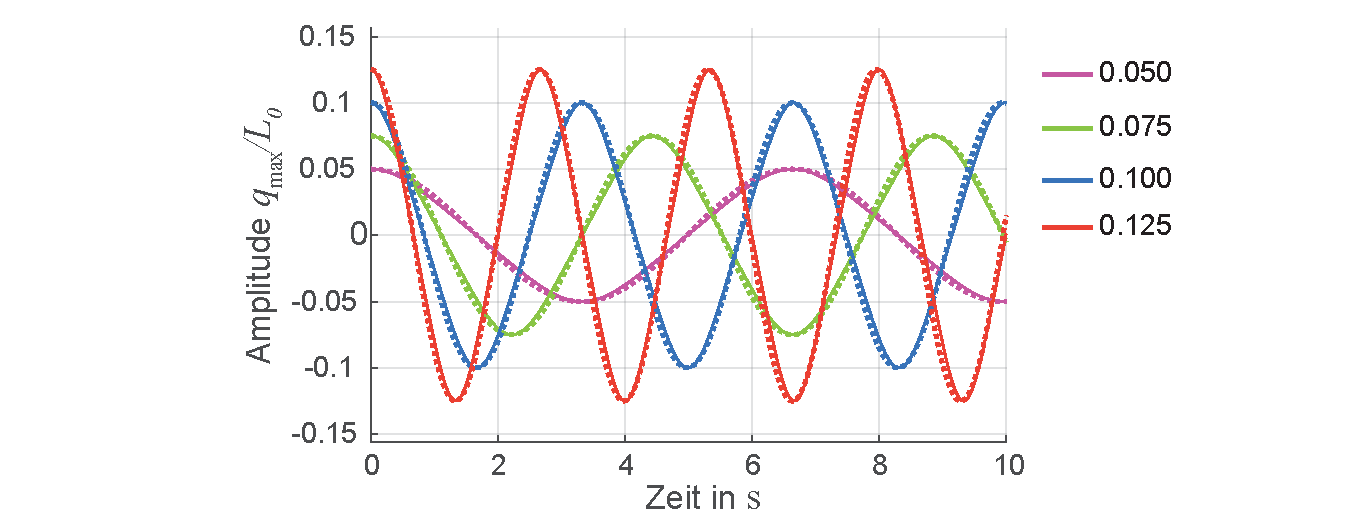
\includegraphics[width=\textwidth]{Expander.pdf}
\caption[Abh�ngigkeit der Schwingungsperiode des Expanders]{Abh�ngigkeit der Schwingungsperiode des Expanders von der relativen Anfangsauslenkung $q_\text{max}/L0$} 
\label{abb:bew_ExpanderLsg}
\end{figure}
    
    \item \glqq Erdfahrstuhl \grqq{} \cite{Mohazzabi2004} \\

     Man kann zeigen (als zus�tzlich �bung empfohlen), dass das Gravitationspotential im Inneren der Erde durch 
            \begin{align}
                U\lk r\rk = \frac{G\,M_\text{E}\,m}{\lk \kappa+2\rk\,R}\,\lk \frac{r}{R}\rk^{\kappa+2} ~~~~ r\leq R_\text{E}\,, \label{eq:bew_NLOUe07}
            \end{align}
    gegeben ist, wenn wir eine ver�nderliche Dichte
            \begin{align}
                \varrho\lk r\rk = \varrho_0\lk \frac{r}{R_\text{E}}\rk^\kappa \label{eq:bew_NLOUe08}
            \end{align}
    annehmen, f�r die $\kappa>-2$ (reell) und $\varrho_0>0$ ist.\footnote{$\kappa=0$ bedeutet konstante Dichte. Eine brauchbare N�herung f�r die Erde ergibt sich nat�rlich nicht durch eine so einfache Beziehung wie \eqref{eq:bew_NLOUe08}, wir werden dann wohl wieder numerisch rechnen m�ssen.} \\
    Wir geben hier f�r zwei F�lle die Beziehung f�r die Schwingungsperiode an. F�r $\kappa=0$ (homogener Fall) ergibt sich logischerweise die harmonische\footnote{Interessanterweise, oder besser logischerweise, entspricht die Schwingungsdauer genau der Erdumrundungszeit eines der Erdoberfl�che nahen Satelliten. (Warum?)} L�sung mit 
            \begin{align*}
                T = 2\pi\,\sqrt{\frac{{R_\text{E}}^3}{G\,M}} = 2\pi\,\sqrt{\frac{R_\text{E}}{g}}\,.
            \end{align*}
    F�r $\kappa=-1$ (zum Kern zunehmende Dichte) ergibt sich ein Potential
            \begin{align*}
                U\lk r\rk = \frac{G\,M_\text{E}\,m}{R^2}\,|r|\,,
            \end{align*}
    was eine konstante Kraft auf den Fahrstuhl bedeutet.
\end{enumerate}

\end{sol} 
%\href{PhysikUncut_Part1.pdf#prb:bew_PendelUeb01}{\textcolor{blue} {$\rightarrow$ zur \probref{bew_PendelUeb01}.}}\\
\textcolor{blue} {$\rightarrow$ zur} \probref{bew_PendelUeb01}.\\
\noindent\rule[1ex]{\textwidth}{0.5pt}  \newpage


%-----------------------------------------------------------------------------------------------------------
\hypertarget{lsg:bew_schaukelI}{}
\begin{sol}{prob:bew_schaukelI}\label{lsg:bew_schaukelI}%�bung35
\textbf{Parametrische Oszillatoren.}\\

Wir wollen den parametrischen Oszillator zun�chst ohne Reibung und ohne Anregung betrachten. Dann k�nnen wir \eqref{eq:bew_schaukel01d} mit $p_1\lk t\rk = 0$ und $p_2\lk t\rk = {\omega(t)}^2 = {\omega_0}^2\,\lk 1+\kappa\,\cos\Omega t\rk$ schreiben als:
        \begin{align}
            \ddot{x} +\omega\lk t\rk^2\,x = 0 \,. \label{eq:bew_ParaOsz01}
        \end{align}
Wir wollen ferner annehmen, dass die parametrische Anregungsfrequenz $\Omega$ in der N�he von $2\omega_0$, also der doppelten Eigenfrequenz, liegt:
        \begin{align}
            \Omega = 2\omega_0+\Delta\omega ~~~~ \text{mit} ~~~~ |\Delta\omega|\ll \omega_0\,. \label{eq:bew_ParaOsz02}
        \end{align}
Ebenso ist $\kappa\ll 1$. \\
Dann folgt aus \eqref{eq:bew_ParaOsz01} die sogenannte Mathieusche\indexp{Mathieu, �mile L�onard}\index{Mathieusche Differentialgleichung}\footnote{�mile L�onard Mathieu (1835--1890) war ein franz�sischer Mathematiker und Physiker, der vor allem auf dem Gebiet der Gruppentheorie arbeitete. In der Physik untersuchte er \ua die Schwingungen von Flocken, das Dreik�rperproblem und die W�rmeleitung.} Differentialgleichung:
        \begin{align}
            \ddot{x} + {\omega_0}^2\,\lk 1 + \kappa\,\cos\lk\Omega t\rk \rk\, x = 0 \,. \label{eq:bew_ParaOsz03}
        \end{align}
Wir machen den Ansatz:
        \begin{align}
            x = A\lk t\rk\,\cos\lk\omega t\rk + B\lk t\rk\,\sin\lk \omega t\rk ~~~~ \text{mit} ~~~~ \omega =  \omega_0 + \frac{\Delta\omega}{2} \,, \label{eq:bew_ParaOsz04}
				\end{align}
und erhalten dann aus \eqref{eq:bew_ParaOsz03}
        \begin{align}
        \begin{split}
            &\ddot{A} + 2\dot{B}\,\omega + A\lk {\omega_0}^2-\omega^2+{\omega_0}^2\,\kappa\,\cos\Omega t\rk\,\cos \Omega t + \ddot{B} - 2\dot{A}\,\omega \\
            &+B\,\lk {\omega_0}^2-\omega^2+{\omega_0}^2\,\kappa\,\cos\Omega t\rk \,\sin\Omega t = 0 \,. \label{eq:bew_ParaOsz05}
        \end{split}
        \end{align}
Wir wollen ja die Umgebung der Resonanz untersuchen und machen daher folgende N�herung f�r die zeitlich langsam ver�nderlichen Gr��en $A\lk t\rk$ und $B\lk t\rk$
        \begin{align}
            \dot{A} &\approx \Delta\omega\,A \,~~  \ddot{A} \approx {\Delta\omega}^2\,A \,~~ \dot{B} \approx \Delta\omega\,B \,~~ \ddot{B} \approx {\Delta\omega}^2\,B \,~~
            \text{und}~~ |\Delta&\omega| < \frac{1}{2}\,\omega_0\,\kappa\,. \label{eq:bew_ParaOsz05a}
        \end{align}
Dann k�nnen wir aus \eqref{eq:bew_ParaOsz05}, wenn wir nur die Glieder erster Ordnung in $\Delta\omega$ mitnehmen, folgende Gleichung ableiten:
        \begin{align}
        \begin{split}
            &\lek 2\dot{B}+A\lk -\Delta\omega+\omega_0\,\kappa\,\cos\Omega t\rk\,\cos\omega t\rek \\
            &+\lek -2\dot{A} + B\lk -\Delta\omega + \omega_0\,\kappa\,\cos\Omega t\rk\,\sin\omega t \rek = 0\,. \label{eq:bew_ParaOsz06}
        \end{split}
        \end{align}
Unter Benutzung von:
        \begin{align*}
            2\cos x\cos y &= \cos\lk x-y\rk + \cos \lk x+y\rk \\
            2\sin x\sin y &= \sin\lk x-y\rk + \sin\lk x+y\rk \,,
        \end{align*}
ergibt sich daraus unter Vernachl�ssigung h�herer Harmonischer von $\omega$:
        \begin{align}
            \lek 2\dot{B}+ A\lk-\Delta\omega+\frac{\omega_0\,\kappa}{2}\rk\rek\,\cos \omega t - \lek 2\dot{A} + B\,\lk +\Delta\omega + \frac{\omega_0\kappa}{2}\rk\rek\,\sin\omega t = 0 \,. \label{eq:bew_ParaOsz07}
        \end{align}
Die eckigen Klammern ergeben ein verkoppeltes linearisiertes DGL-System in $A\lk t \rk$ und $B\lk t \rk$, das man mit dem Ansatz $A = A_0\,\e^{\lambda\,t}$ und $B = B_0\,\e^{\lambda\,t}$ l�sen kann. \\
Man erh�lt dann das bestimmende Gleichungssystem
        \begin{align}
        \begin{split}
            \frac{A_0}{2}\,\lk \frac{\omega_0\,\kappa}{2} - \Delta\omega\rk + B_0\,\lambda &= 0  \,, \\
            A_0\,\lambda+ \frac{B_0}{2}\,\lk\frac{\omega_0\,\kappa}{2}+ \Delta\omega\rk &= 0 \,. \label{eq:bew_ParaOsz08}
        \end{split}
        \end{align}
Das System hat nur dann L�sungen f�r $A_0$ und $B_0$, wenn $\frac{1}{4}\lk\frac{{\omega_0}^2\,\kappa^2}{2}-\Delta\omega^2\rk - \lambda^2 = 0$ ist, was auf 
        \begin{align}
            \lambda_{+,-} = \pm \frac{\Delta\omega}{2}\sqrt{\frac{{\omega_0}^2\,\kappa^2}{4\Delta\omega^2}-1} \label{eq:bew_ParaOsz09}
        \end{align}
f�hrt. Wenn wir ein Anwachsen der Amplitude beobachten wollen, brauchen wir nur $\lambda_+$ zu ber�cksichtigen und m�ssen fordern, dass $|\Delta\omega|<\omega_0\,\kappa /2$ ist, da sonst die Wurzel imagin�r wird. Allerdings darf $\omega_0\,\kappa / \lk 2|\delta\omega| \rk$ nicht sehr viel gr��er als $1$ werden, da sonst die N�herung \eqref{eq:bew_ParaOsz05a} nicht mehr erf�llt ist. \\
Wir sehen also f�r kleine $\Delta\omega$ ein exponentielles Anwachsen der Amplitude mit 
        \begin{align*}
            x\lk t\rk &= A_0\,e^{\lambda\,t}\,\cos\omega t + B_0\,e^{\lambda\,t}\,\sin\omega t = e^{\lambda\,t}\,\lk A_0\,\cos\omega t + B_0\,\sin\omega t\rk \\
            \text{mit} ~~~~ \lambda &= \frac{1}{2}\sqrt{\frac{{\omega_0}^2\,\kappa^2}{4}-\Delta\omega^2}
        \end{align*}
und f�r die Anfangsbedingungen $B_0= B\lk 0 \rk = 0$ und $A_0 \neq 0$ (aber sehr klein) ergibt sich das bereits bekannte exponentielle \glqq Aufschaukeln \grqq. \\
In \figref{bew_paraOsz01} zeigen wir diese N�herungsl�sung als auch die numerische L�sung f�r verschiedene Frequenzmismatches $|\Delta\omega| = |2\omega_0-\Omega|$. Ebenso stellen wir die numerische L�sung f�r den getriebenen Oszillator mit Reibung dar. 

\begin{figure}[H]\centering
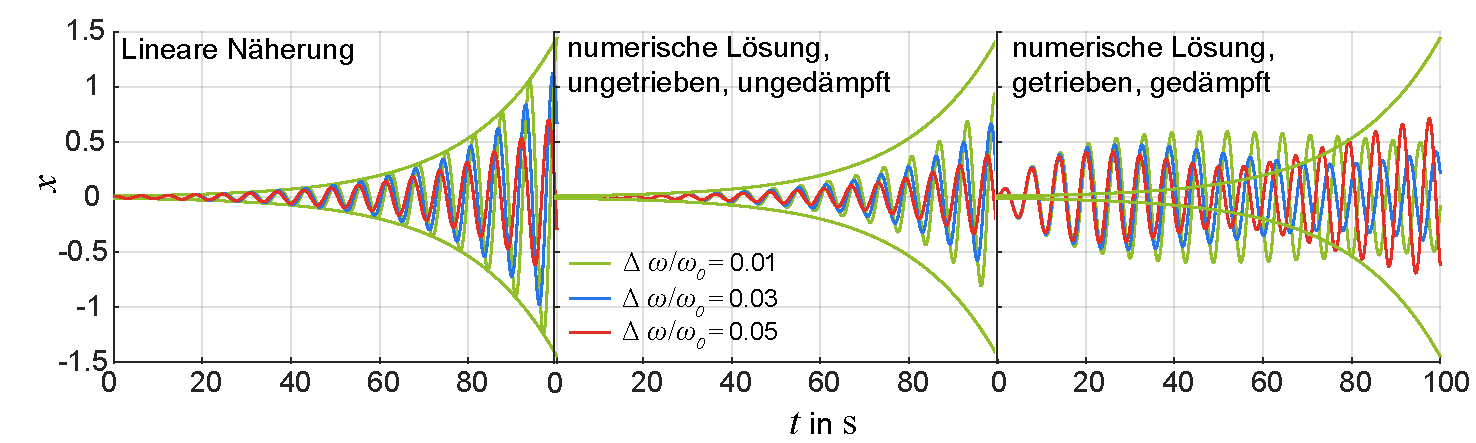
\includegraphics[width=\textwidth]{ParaOsz01.pdf}%
\caption[Dynamik eines parametrischen Oszillators]{Dynamik des parametrischen Oszillators. a) L�sung des linearisierten Problems f�r den unged�mpften, ungetriebenen Fall. Man erkennt den exponentiellen Anstieg, der typisch f�r einen parametrischen Oszillator ist. Die Eigenfrequenz wird mit $2\omega_0 + \Delta\omega$ moduliert. b) Numerische L�sung  f�r den unged�mpften, ungetriebenen Fall. Man erkennt, dass durch die Ber�cksichtigung der h�heren Terme in der Modulation die Amplitude langsamer anw�chst. c) Numerische L�sung  f�r den ged�mpften, getriebenen Fall. Die Anregung erfolgt hier mit $\omega_0 + \Delta\omega$ . Sie stellt den dominanten Einfluss dar und ist f�r die Dynamik ausschlaggebend}
\label{abb:bew_paraOsz01}
\end{figure}

\end{sol} 
%\href{PhysikUncut_Part1.pdf#prb:bew_schaukelI}{\textcolor{blue} {$\rightarrow$ zur \probref{bew_schaukelI}.}}\\
\textcolor{blue} {$\rightarrow$ zur} \probref{bew_schaukelI}.\\
\noindent\rule[1ex]{\textwidth}{0.5pt}  \newpage

%-----------------------------------------------------------------------------------------------------------
\hypertarget{lsg:bew_schaukelII}{}
\begin{sol}{prob:bew_schaukelII}\label{lsg:bew_schaukelII}%�bung36
\textbf{Betrachtungen zur Schaukel.}\\
\begin{enumerate}[a)]
\item
  Wir benutzen vorteilhaft die \matlab{} Symbolic Math Toolbox.
  Details der Berechnung sind in \mlbewref{SchaukelLG.m} angegeben.
\item 
Man entwickle die Funktionen $\sin\psi(t) =\sin \lk \psi_0\, \cos\omega t \rk $ und $\cos\psi(t) =\cos \lk \psi_0\, \cos\omega t \rk $  in der Lagrange-Gleichung \eqref{eq:bew_schaukel17a} bis zur dritten Ordnung und ber�cksichtige in der erhaltenen Beziehung nur die Terme mit Frequenzen $\omega$ und $2\omega$. Details der Rechnung sind auch in \cite{Case1990} zu finden.
\item
Wir modellieren die schaukelnde Person als festen K�rper mit dem Tr�gheitsmoment $m\,H^2$ (zugegeben ein etwas untersetzter Schaukler!). Der Auslenkungswinkel der Schaukel ist wieder $\theta$ und die Neigung des (starren) K�rper gegen die Pendelstange $\psi$. Wir nehmen wieder an, dass die Person harmonisch schwingt mit $\psi = \psi_0\,\cos\omega t$. \\
Man kann unter Beachtung, dass der Schwerpunkt $S$ einen Abstand $s$ vom Brett der Schaukel hat, die Lagrange-Funktion relativ einfach aufstellen, wenn man ber�cksichtigt, dass die Person (d.\,h. ihr Schwerpunkt) sich mit der Winkelgeschwindigkeit ($\dot{\theta}+\dot{\psi}$) gegen�ber der Aufh�ngung bewegt:
        \begin{align}
        \begin{split}
            \mathcal{L} = &\frac{1}{2}\,m\lek L^2\,\dot{\theta}^2 - 2L\,s\,\dot{\theta}\,\lk \dot{\theta} + \dot{\psi}\rk \,\cos\psi + \lk s^2 + H^2\rk\lk\dot{\theta} +\dot{\psi}\rk^2\rek\\
            &+ m\,g \lek L\,\cos\theta - s\,\cos\lk \theta+\psi\rk\rek \,. \label{bew_StandingSwing01}
        \end{split}
        \end{align}
Daraus folgt die Bewegungsgleichung f�r $\theta$ (\matlab{} Symbolic ToolBox)
        \begin{align}
        \begin{split}
            \lek L^2-2L\,s\,\cos\psi + s^2 + H^2\rek\,\ddot{\theta} = &-g\,L\,\sin\theta + g\,s\,\sin\lk\theta+\psi\rk - L\,s\,\sin\psi\,{\dot{\psi}}^2 \\
            &+ \lk L\,s\,\cos\psi - s^2+H^2\rk\,\ddot{\psi} - 2L\,s\,\sin\psi\,\dot{\theta}\,\dot{\psi} \,.\label{bew_StandingSwing02}
        \end{split}
        \end{align}
Wir k�nnen \eqref{bew_StandingSwing02} numerisch l�sen, wiederum mit $\psi=\psi_0\,\cos\omega t$. Ebenso wir k�nnen die Bewegungsgleichung f�r kleine Winkel $\psi$ entwickeln. Bis zur zweiten Ordnung von $\psi$ ergibt sich:
        \begin{align}
        \begin{split}
            \lek \lk L-s\rk^2+H^2 + L\,s\,\psi^2\,\rek \ddot{\theta} + 2L\,s\,\psi\,\dot{\psi}\,\dot{\theta} + \lek g\lk L-s\rk\, + \lk\frac{g\,s}{2}\rk\,\psi^2\, \rek \theta \\
						=  g\,s\,\psi+\lek s\lk L-s\rk-H^2\rek\,\ddot{\psi}\,.\label{bew_StandingSwing03}
        \end{split}
        \end{align}
Wir erkennen wieder die DGL eines harmonischen Oszillators mit zwei Treibertermen und wiederum zeitabh�ngige Modifikationen der Eigenfrequenz, D�mpfung und des Tr�gheits-/Massenmoments (Terme vor $\theta$, $\dot{\theta}$ und $\ddot{\theta}$). \\
Die weitere Rechnung ist analog dem Vorgehen in \kapitel{bew_pendulum_param}.

\end{enumerate}
\end{sol} 
%\href{PhysikUncut_Part1.pdf#prb:bew_schaukelII}{\textcolor{blue} {$\rightarrow$ zur \probref{bew_schaukelII}.}}\\
\textcolor{blue} {$\rightarrow$ zur} \probref{bew_schaukelII}.\\
\noindent\rule[1ex]{\textwidth}{0.5pt}  \newpage

%-----------------------------------------------------------------------------------------------------------
\hypertarget{lsg:bew_schaukelIII}{}
\begin{sol}{prob:bew_schaukelIII}\label{lsg:bew_schaukelIII}%�bung37
\textbf{�berschlag.}\\

Bisher haben wir die Schaukelaufh�ngung immer als starr angenommen. Das muss aber nicht sein, wir wollen jetzt eine Kette als Aufh�ngung annehmen. \\
Wir m�ssen dann die Spannung in der Kette ber�cksichtigen. Diese ist mit der Bewegung und damit der Zeit ver�nderlich.
In Seilrichtung wirkt die Zugkraft aus Zentrifugalkraft
        \begin{align*}
            \vec{F}_\text{Z} = - \frac{v^2}{L} \,\vec{e}_r = -\frac{\dot{x}^2 + \dot{z}^2}{L}\,\vec{e}_r \left\}\,\rightarrow
            \begin{array}{ll}
            \vec{F}_\text{Zx} = -\frac{\dot{x}^2 + \dot{z}^2}{L}\,\sin\theta\,\veceX\\
            \vec{F}_\text{Zy} = -\frac{\dot{x}^2 + \dot{z}^2}{L}\,\cos\theta\,\veceZ\\
            \end{array}
            \right. 
        \end{align*}
und einem Anteil der Gewichtskraft
        \begin{align}
            \vec{F}_\text{G} &= m\,g\,\veceZ = -m\,g\,\cos\theta\,\vec{e}_r - m\,g\,\sin\theta\,\vec{e}_\theta \,\rightarrow
            \begin{array}{ll}
            \vec{F}_\text{Gx} = -m\,g\,\cos\theta\,\sin\theta \,\veceX\\
            \vec{F}_\text{Gy} = -m\,g\,\cos^2\theta \,\veceZ\\
            \end{array} \,. \label{eq:bew_ueberschlag01}
        \end{align}
Die Bewegungsgleichung f�r die Masse $m$ (wir haben f�r diese Betrachtung die Masse des Schaukelnden in dem Sitz verdichtet.) lautet dann:
        \begin{align}
            \begin{pmatrix}
                \ddot{x}\\
                \ddot{z}
            \end{pmatrix}
            =
            \begin{pmatrix}
                -\frac{\dot{x}^2 + \dot{z}^2}{L}\,\sin\theta & ~~-g\,\sin\theta\,\cos\theta \\
                 -\frac{\dot{x}^2 + \dot{z}^2}{L}\,\cos\theta & ~~-m\,g\,\lk \underbrace{1-\sin^2\theta}_{\cos^2\theta} \rk
            \end{pmatrix}
            \,. \label{eq:bew_ueberschlag02}
        \end{align}
Diese Bewegungsgleichung gilt nur, so lange die Kette gespannt ist. Der jeweils erste Term beschreibt die wirkende Zentrifugalkraft in $x-$ und $z-$Richtung, der zweite Term den Beitrag der Gewichtskraft zur Kettenspannung
Wir sehen, dass die $x-$Komponente der Gewichtskraft die Zentrifugalkraftkomponente der Kettenspannung bis zu einem Winkel $\theta = 90\degree$ erh�ht (Betrachtung im mitbewegten System), f�r $\theta > 90\degree$ aber wirkt der Beitrag von $\vec{F}_\text{z,x}$ in positive $x-$Richtung (wegen $\cos\theta<0$), so dass bei einem Winkel $\theta_\text{max}$ die $x-$Komponente der Zugkraft Null wird:
        \begin{align}
            &0 = -\frac{\dot{x}^2 + \dot{z}^2}{L}\,\sin\theta_\text{A} - g\,\sin\theta_\text{A}\,\cos\theta_\text{A} \nonumber \\
            &\rightarrow \cos\theta_\text{A} =  -\frac{\dot{x}^2 + \dot{z}^2}{g\,L} ~~~~ \rightarrow ~~~~ \theta_\text{A} > 90\degree \label{eq:bew_ueberschlag03}
        \end{align}
In \figref{bew_ueberschlag02} ist das Ergebnis der numerischen Simulation von \eqref{eq:bew_ueberschlag02} gezeigt, man erkennt, dass ab $\theta > \theta_\text{A}$ die Schaukel in eine ballistische Bahn mit den Anfangswerten
        \begin{align*}
            \begin{pmatrix}
            x\lk \theta_\text{A}\rk\\
            z\lk \theta_\text{A}\rk\
            \end{pmatrix}
            ~~~~
            \text{und}
            ~~~~
             \begin{pmatrix}
            \dot{x}\lk \theta_\text{A}\rk\\
            \dot{z}\lk \theta_\text{A}\rk\\
            \end{pmatrix}
        \end{align*}
�bergeht. Wir haben in \figref{bew_ueberschlag02} auch verschiedene Anfangsbedingungen
        \begin{align*}
            \dot{x}\lk 0\rk = v_0, \,x\lk 0\rk = 0, \,\dot{z}\lk 0\rk = 0,\,z\lk 0\rk = - L
        \end{align*}
simuliert. Ebenso ist die Geschwindigkeit beim Auftreffen am Punkt $P_\text{E}$ gekennzeichnet, an welchem der Schaukler eine gro�e Abbremsbeschleunigung (abh�ngig von der Elastizit�t an der Kette erf�hrt). 

\begin{figure}[H]\centering
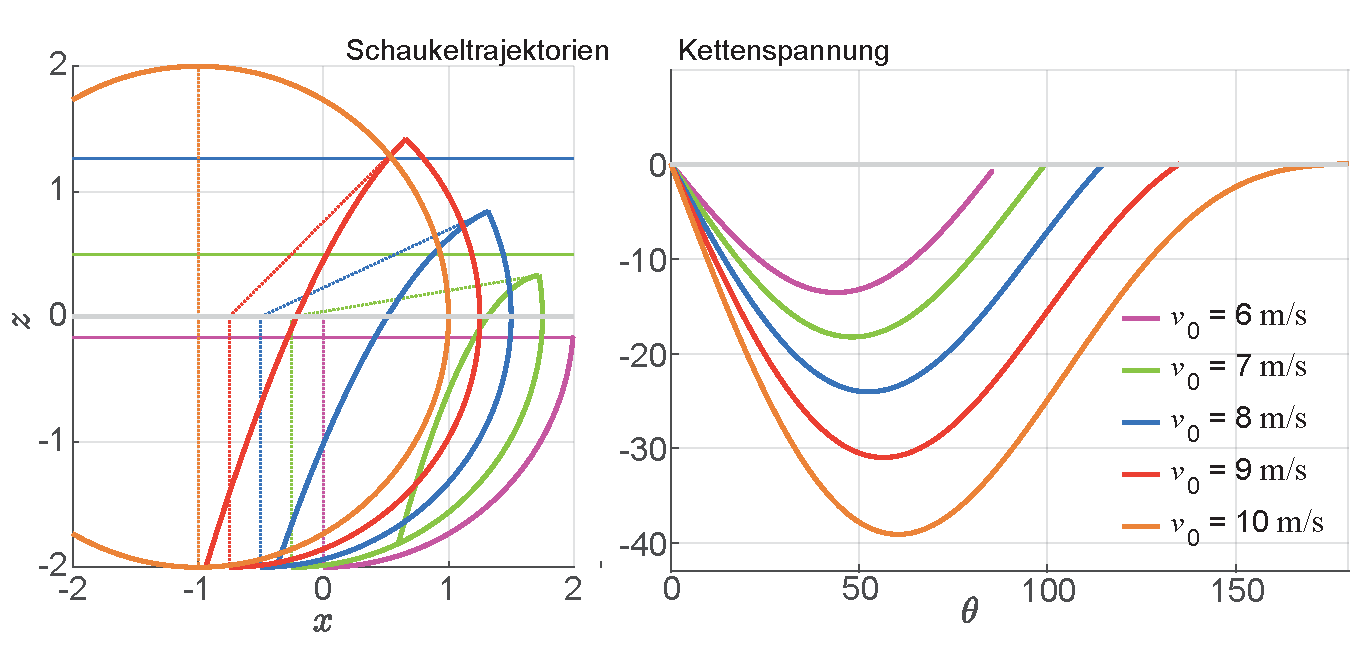
\includegraphics[width=\textwidth]{SchaukelUeberschlag.pdf}%
\caption[Schaukel�berschlag]{Schaukel�berschlag. Trajektorien und Kettenspannung als Funktion des Winkels $\theta$}
\label{abb:bew_ueberschlag02}
\end{figure}

Aus der Betrachtung der Energieerhaltung kann man noch eine einfache Formel f�r den Winkel $\theta_\text{A}$ herleiten:
        \begin{align}
            \theta_\text{A} = 90\degree +\arcsin \lek\frac{1}{3}\lk \frac{{v_0}^2}{g\,L}-2\rk\rek\,, \label{eq:bew_ueberschlag04}
        \end{align}
die wir empfehlen nachzurechnen (siehe auch \cite{Bickel2019}). \\
Wir empfehlen auch zur �bung die vorstehenden Rechnungen unter Benutzung der Lagrange-Multiplikatoren zu wiederholen. Die Lagrange-Funktion kann aufgeschrieben werden zu:
        \begin{align*}
            \mathcal{L}\lk x,\dot{x},z,\dot{z}\rk = T\lk \dot{x},\dot{z}\rk - U\lk x,z\rk + \lambda\,f
        \end{align*}
Bei der L�sung der Lagrange-Gleichung muss der Vorzeichenwechsel des Lagrange-Multiplikators betrachtet werden, danach gilt keine Zwangsbedingung mehr. Die Zwangsbedingung ist gegeben durch
        \begin{align*}
            f = x^2 + y^2 - L =0 \,.
        \end{align*}
\newpage
\begin{nebenrechnung}
~~Herleitung von Gleichung \eqref{eq:bew_ueberschlag01} (alles auf Masse $m$ bezogen):
        \begin{align*}
            \vec{F}_{T_{1}} &= -\vec{F}_\text{Zentr} = -\frac{v^2}{L}\,\lek \cos\lk 90\degree-\theta\rk\,\veceX+ \sin \lk 90\degree-\theta\rk\,\veceZ \rek \\
						&= -\frac{v^2}{L}\,\vec{e}_r = -\frac{v^2}{L}\,\sin\theta\,\veceX + \cos\theta\,\veceZ \,, \\
            \vec{F}_\text{ges} &= \vec{F}_{T_{1}} +\vec{F}_{T_{2}} + \vec{G}\,,  ~~~~~~~~~ \vec{G} = -g\,\veceZ\,, \\
            \vec{F}_{T_{2}} &= -\vec{G}_\text{rad} = -\lek-g \lk \veceZ\cdot\vec{e}_r\rk\veceX\rek = +g\,\cos\theta\,\vec{e}_r = +g\,\cos\theta \lk\sin\theta\,\veceX+\cos\theta\,\veceZ\rk \,, \\
            \begin{pmatrix}
            \ddot{x} \\
            \ddot{z}
            \end{pmatrix}
            &=
            \begin{pmatrix}
            -\frac{v^2}{L}\,\sin\theta & -g\,\sin\theta\,\cos\theta\\
            -\frac{v^2}{L}\,\cos\theta & +g\,\cos^2\theta-g
            \end{pmatrix} = 
            \begin{pmatrix}
            -\frac{v^2}{L}\,\sin\theta & -g\,\sin\theta\,\cos\theta\\
            -\frac{v^2}{L}\,\cos\theta & -g\,\sin^2\theta
            \end{pmatrix} \,.
						\,.
        \end{align*} 
\end{nebenrechnung}
\end{sol} 
%\href{PhysikUncut_Part1.pdf#prb:bew_schaukelIII}{\textcolor{blue} {$\rightarrow$ zur \probref{bew_schaukelIII}.}}\\
\textcolor{blue} {$\rightarrow$ zur} \probref{bew_schaukelIII}.\\
\noindent\rule[1ex]{\textwidth}{0.5pt}  \newpage

%-----------------------------------------------------------------------------------------------------------
\hypertarget{lsg:bew_PendelUeb03}{}
\begin{sol}{prob:bew_PendelUeb03}\label{lsg:bew_PendelUeb03} %�bung38
\textbf{Das invertierte Pendel.} \\ \\
Wir folgen hier der Darstellung in \cite{Butikov2001}. Die Position der Masse ist nach \figref{bew_InversPendel01} gegeben durch:
\begin{align}
    x = L\,\sin\theta\,, ~~~~ z = z_\text{B} + L\,\cos\theta\,,  \label{eq:bew_InversPendel01}
\end{align}
worin $z_\text{B}\lk t\rk$ eine beliebige Bewegung der Basis des invertierten Stangenpendels ist . \\
Dann folgt mit  
\begin{align}
    \dot{x} &= L\,\dot{\theta}\,\cos\theta\,, ~~~~ \dot{z} = \dot{z}_\text{B}\,-L\,\dot{\theta}\,\sin\theta  ~~\text{und}\nonumber \\
     v^2 = L^2\,\dot{\theta}^2 + \dot{z}_\text{B}{}^2 - 2L\,\dot{z}_\text{B}\,\dot{\theta}\,\si\theta\,. \label{eq:bew_InversPendel02}
\end{align}
die Lagrange-Funktion 
\begin{align}
    \mathcal{L} = \frac{1}{2}\,m\,\lk L^2\,\dot{\theta}^2 + \dot{z}_\text{B}{}^2 - 2L\,\dot{z}_\text{B}\,\dot{\theta}\,\sin\theta\rk -m\,g\,z\,\lk z_\text{B} + L\,\cos\theta\rk \, \label{eq:bew_InversPendel03}
\end{align}
und daraus die Bewegungsgleichung f�r $\theta$:
\begin{align}
     L\,\ddot{\theta} - \ddot{z}_\text{B}\,\sin\theta - g\,\sin\theta = 0\,.         \label{eq:bew_InversPendel04}
\end{align}

\begin{figure}
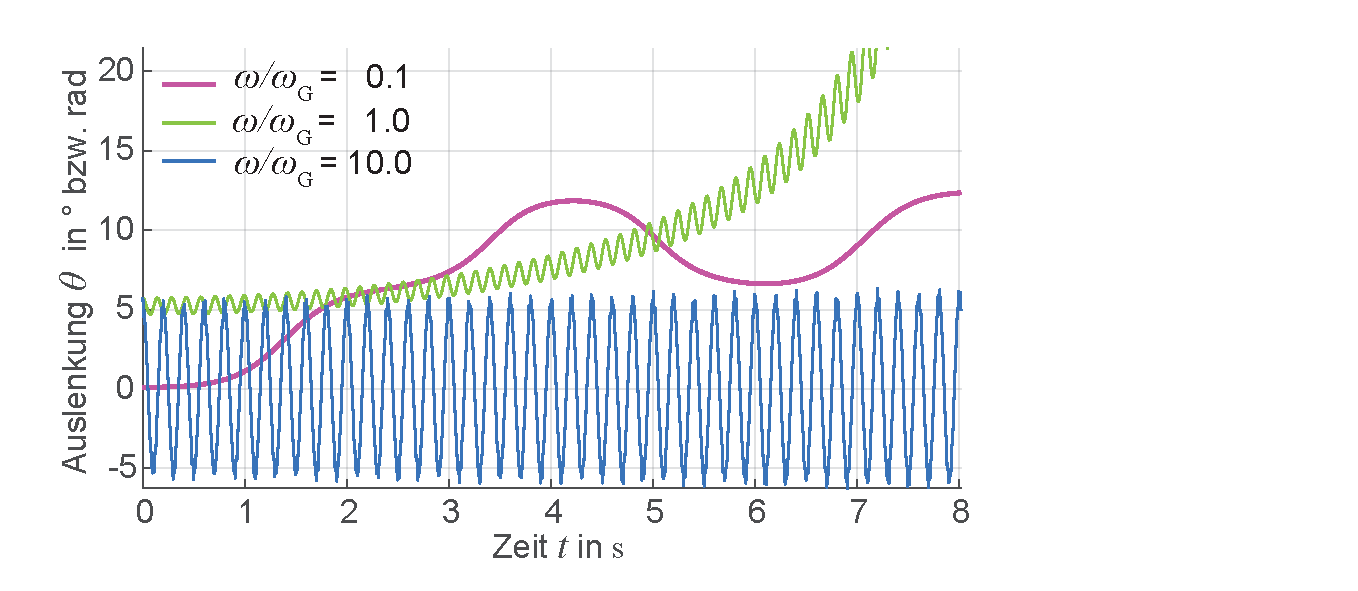
\includegraphics[width=\textwidth]{InversPendel02.pdf}
\caption[Das invertierte Pendel f�r verschiedene Anregungsfrequenzen.]{Das invertierte Pendel f�r verschiedene Anregungsfrequenzen. Parameter: $L=\SI{1.0}{\metre}, a=A/L=0.1, \theta_0 = 0.1 \mathrm{rad}, \omega_G^2 = 2\omega_0^2/a^2$. Man beachte, dass die Kurve f�r $\omega = 0.1\omega_0$ in Einheiten von rad ist, f�r die beiden anderen Kurven ist die vertikale Achse in Einheiten von $\degree$ dargestellt. Man sieht, dass f�r $\omega > 10\omega_0$ eine dynamische Stabilisierung erfolgt} 
\label{abb:bew_InversPendel02}
\end{figure}

Gegen�ber einem \glqq normalen \grqq{} Stangenpendel kann man die \glqq r�cktreibende\grqq{} Gewichtskraft als durch $\ddot{z}_\text{B}\lk t\rk$ moduliert ansehen. \\
Wir k�nnen f�r $z_\text{B}\lk t\rk$ jede beliebige zeitliche Funktion annehmen, und dann \eqref{eq:bew_InversPendel04} numerisch l�sen (\figref{bew_InversPendel02}), wollen aber zun�chst f�r $z_\text{B}\lk t\rk$ einen harmonischen Verlauf annehmen und damit auch eine analytische N�herung probieren:
\begin{align*}
    z_\text{B}\lk t\rk &= A\,\cos(\omega t) \,,~~~~ \ddot{z}_\text{B} \lk z\rk = -\omega^2\,A\,\cos(\omega t)\,.
\end{align*}

\newpage
Damit wird aus \eqref{eq:bew_InversPendel04}:
\begin{align}
    \ddot{\theta} + \sin(\theta)\,\lk a\,\omega^2\,\cos\lk \omega t\rk - \omega_0{}^2\rk = 0\,.\label{eq:bew_InversPendel05}
\end{align}
Wenn man bei fester L�nge $L$ und Anregungsamplitude $A$ die Anregungsfrequenz $\omega$ in weitem Bereich durchstimmt, so findet man ein interessantes Verhalten. Bei kleiner Anregungsfrequenz $\omega$ wird der Pendelstab aus seiner urspr�nglichen Anfangslage $\theta > 0$ (aber sehr klein) umfallen und je nach Anregungsst�rke zwischen $\theta = \pi/2$ und $\theta = 3\pi/2$ hin- und herpendeln oder aber auch �berschl�ge machen. Bei deutlich h�heren Anregungsfrequenzen kommt es aber zu einer interessanten Stabilisierung von hochfrequenten Schwingungen um die Nulllage ($\theta \approx 0$) (\figref{bew_InversPendel02}). Wie kann man das physikalisch erkl�ren?\\
Wir gehen zu kleinen Winkeln $\theta$ �ber und schreiben die Bewegungsgleichung als:
\begin{align}
    \ddot{\theta} + \theta\,\lk a\,\omega^2\,\cos(\omega t)- \omega_0{}^2\rk = 0 ~~~~ \text{mit} ~~~~ a = \frac{A}{L}\,, ~~~~ \omega_0{}^2 = \frac{g}{L}\,. \label{eq:bew_InversPendel06}
\end{align}
Da sich die mittlere Position des unteren Stabendes nur wenig bewegt, k�nnen wir einen N�herungsansatz f�r die L�sung $\theta\lk t\rk$ machen, indem wir schreiben
\begin{align}
    \theta\lk t\rk = C + D\,\cos(\omega t) ~~~~ \text{mit} ~~~~ D \ll C \,. \label{eq:bew_InversPendel07}
\end{align}
Wir setzen diese N�herungsannahme in \eqref{eq:bew_InversPendel06} ein und erhalten mit $a\ll 1$ (kleine Auslenkung), $a\,\omega^2 \gg \omega_0{}^2$ (hohe Frequenzen) die Beziehung 
\begin{align}
\begin{split}
    &\lk -D + C\,a\rk\,\omega^2\,\cos(\omega t) = 0\\
    \rightarrow ~~~~ &D = C\,a \\
    \rightarrow ~~~~ &\theta\lk t\rk = C\,\lk 1+a\,\cos(\omega t) \rk
\end{split} \label{eq:bew_InversPendel08}
\end{align}
Wir wollen nun eine Zeitentwicklung f�r $t \gg T = 2\pi/\omega$ betrachten. Dazu mitteln wir zeitlich �ber die DGL \eqref{eq:bew_InversPendel06}. 
\begin{align*}
    \overline{\ddot{\theta}}^{\,t} = \overline{-\theta\,\lek a\,\omega^2\,\cos(\omega t) - \omega_0{}^2\rek}^{\,t}\,.
\end{align*}
Mit der N�herung \eqref{eq:bew_InversPendel08} erhalten wir
\begin{align}
\begin{split}
    \overline{\ddot{\theta}}^{\,t} &\approx \overline{-C\lek 1+ a\,\cos\omega t\rek\lek a\,\omega^2\,\cos\omega t - \omega_0{}^2\rek}^{\,t} \\
    &\approx -C\lek a^2\,\omega^2\,\overline{\cos^2\omega t}^{\,t} - \omega_0{}^2\rek \\
    &\approx -C\underbrace{\lek \frac{a^2\,\omega^2}{2}-\omega_0{}^2\rek}_{\substack{\Omega_\text{eff}{}^2}}
\end{split} \label{eq:bew_InversPendel09}
\end{align}
Wir k�nnen die mittlere zeitliche Entwicklung des invertierten Pendels also durch folgende DGL beschreiben:
\begin{align}
    \overline{\ddot{\theta}}^{\,t} = - C\,\Omega_\text{eff}{}^2 = 0 \,. \label{eq:bew_InversPendel10}
\end{align}

\newpage
Andererseits ist die zweite Zeitableitung von \eqref{eq:bew_InversPendel07} wieder zeitlich gemittelt:
\begin{align*}
    \dot{\theta} &= \dot{C} - \dot{D}\,\cos\omega t + \omega\,D\,\sin\omega t \,,\\
    \ddot{\theta} &= \ddot{C} - \ddot{D}\,\cos\omega t + 2\omega\,\dot{D}\,\sin\omega t + \underbrace{ \omega^2\,D\,\cos^2 \omega t }_{\substack{\approx 0}} \,, \\
    \overline{\ddot{\theta}}^{\,t} &= \ddot{C} - \ddot{D}\,\underbrace{\overline{\cos\omega t}^{\,t}}_{\substack{0}} + 2\omega\,\dot{D}\,\underbrace{\overline{\sin\omega t}^{\,t}}_{\substack{0}} \\
		\rightarrow \ddot{\theta} &= \ddot{C} 
\end{align*}
Damit finden wir schlussendlich:
\begin{align}
    \theta\lk t\rk \approx C\lk t\rk \lk 1+a\,\cos\omega t\rk \nonumber \\
    \ddot{C}\lk t\rk + \Omega_\text{eff}{}^2\,C\lk t\rk = 0 \nonumber \\
    \rightarrow C\lk t\rk = C_0\,\cos\lk \Omega_\text{eff}\,t + c_0\rk \label{eq:bew_InversPendel11}
\end{align}
Damit haben wir eine Erkl�rung f�r die relativ stabile, kleine Schwingung um die Nulllage mit der Frequenz $\omega$ und einer entsprechenden Amplitudenmodulation $C\lk t\rk$ mit der Frequenz $\Omega_\text{eff}$. \\
F�r sehr gro�e Frequenzen $\omega^2 \gg \omega_0{}^2$ wird $\Omega_\text{eff} = \frac{a\,\omega}{\sqrt{2}}$, bei $\frac{a^2\,\omega^2}{2} = \omega_0$ bricht unsere N�herung zusammen. Die numerischen Rechnungen sind in den \mscren\mlbewref{InvertiertesPendel01.m} und \mlbewref{InvertiertesPendel02.m} ausgef�hrt und best�tigen unsere analytischen �berlegungen, siehe \figref{bew_InversPendel02} und \figref{bew_InversPendel03}.
\begin{figure}
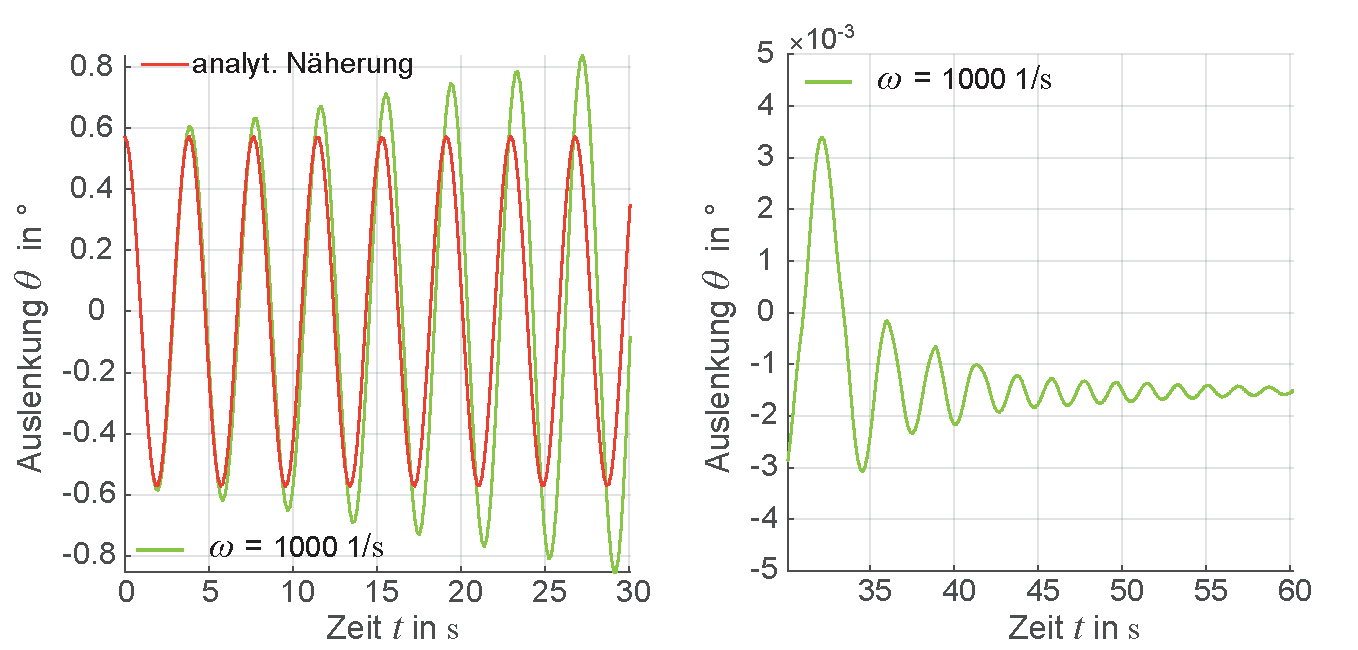
\includegraphics[width=\textwidth]{InversPendel03.pdf}
\caption[Das invertierte Pendel mit und ohne D�mpfung]{Das invertierte Pendel mit und ohne D�mpfung. Parameter: $L=\SI{1.0}{\metre}, a=A/L=0.005, \theta_0 = 0.1 \mathrm{rad}, \omega = \SI{1000}{\per\second}, \Omega_\text{eff} = \SI{1.64}{\per\second}, T_\text{eff} = \SI{3.83}{\second}$. Man beachte, dass die Kurve f�r den ged�mpften Fall f�r einen anderen Zeitbereich dargestellt ist. Das anf�ngliche Schwingungsverhalten wurde ausgeblendet. Deutlich zu erkennen ist die Bedeutung der D�mpfung f�r die dynamische Stabilisierung} 
\label{abb:bew_InversPendel03}
\end{figure}
Wir empfehlen zur Ber�cksichtigung der Reibung und zur Vertiefung die exzellente Darstellung in \cite{Butikov2001}.

\end{sol} 
%\href{PhysikUncut_Part1.pdf#prb:bew_PendelUeb03}{\textcolor{blue} {$\rightarrow$ zur \probref{bew_PendelUeb03}.}}\\
\textcolor{blue} {$\rightarrow$ zur} \probref{bew_PendelUeb03}.\\
\noindent\rule[1ex]{\textwidth}{0.5pt}  
\newpage

%-----------------------------------------------------------------------------------------


%%%-----------------------------------------------------------------------------------------------------------
%%%-----------------------------------------------------------------------------------------------------------
\newpage
\subsection{�bungen zu Grundlagen der Mechanik des starren K�rpers}
\medskip

%-----------------------------------------------------------------------------------------
\hypertarget{lsg:bew_LomegaJ}{}
\begin{sol}{prob:bew_LomegaJ}\label{lsg:bew_LomegaJ} %�bung39
\textbf{Wahl des KOS -- Wirkung auf Drehimpuls, Rotationsgeschwindigkeit, Drehmoment und Tr�gheitstensor.} \\ 
\begin{figure}[H]\centering
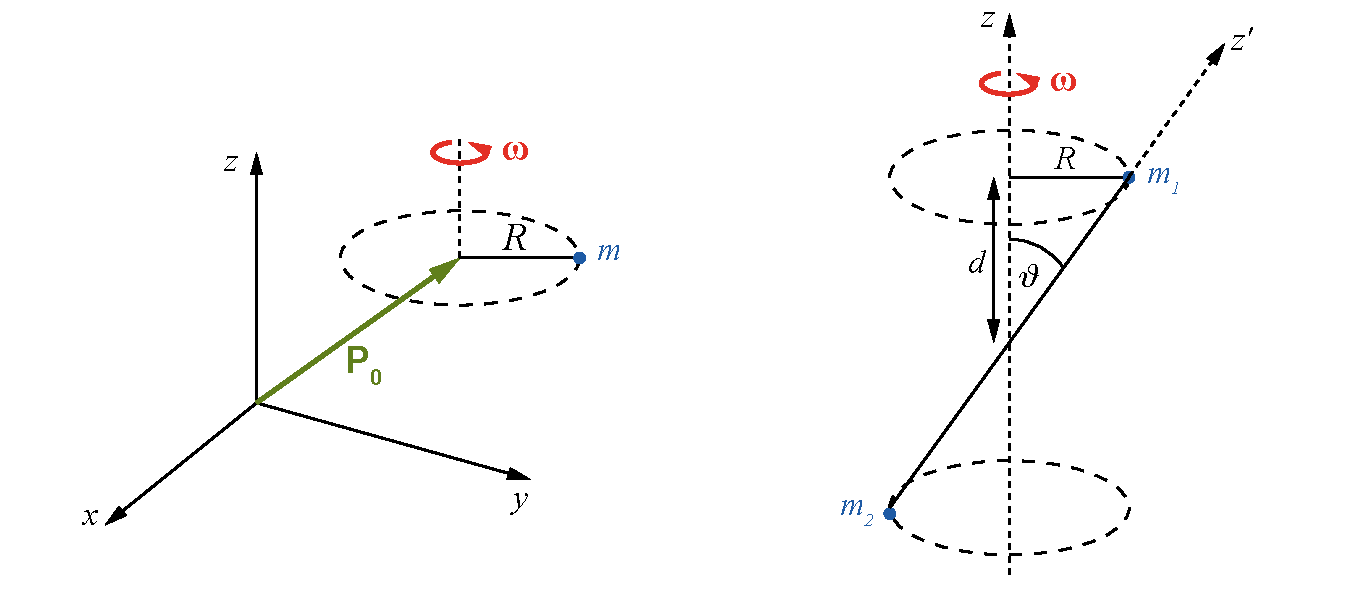
\includegraphics[width=\textwidth]{LomegaJ.pdf}
\caption[KOS-Abh�ngigkeit von Drehimpuls, Rotationsgeschwindigkeit]{Zur KOS-Abh�ngigkeit von Drehimpuls, Rotationsgeschwindigkeit, Drehmoment und Tr�gheitstensor} 
\label{abb:bew_LomegaJ01}
\end{figure}

Wir wollen die Beziehungen zwischen $\vec{L}$, $\vec{\omega}$ und $\vec{\Theta}$ in Abh�ngigkeit vom gew�hlten KOS an zwei einfachen Beispielen veranschaulichen (\figref{bew_LomegaJ01}) (\cite{Silva2007}):
\begin{enumerate}
    \item Massepunkt auf Kreisbahn und
    \item Hantel um ihren Schwerpunkt rotierend.\\
\end{enumerate}
Wir betrachten zun�chst den Massepunkt auf der Kreisbahn und zeigen, dass Drehimpuls und auch Tr�gheitstensor von der Wahl des Koordinatensystems abh�ngen. 
\begin{enumerate}
    \item 
    \begin{enumerate}
        \item [a)] \emph{Das KOS habe seinen Ursprung in einem beliebigen Punkt $P_0$.}
        \begin{align*}
            \vec{P}_0 &= x_0\,\veceX+y_0\,\veceY + z_0\,\veceZ \,,~~~\vec{\omega} = \omega\,\veceZ \,.
        \end{align*}
        \begin{align}
				\vec{x} &= 
            \begin{pmatrix}
            \lk x_0 + R\,\cos\omega t\rk\\
            \lk y_0 + R\,\sin\omega t\rk \\
            z_0
            \end{pmatrix} \,,~~~
            \dot{\vec{x}} = 
            \begin{pmatrix}
            -\omega\,R\,\sin\omega t \\
            \omega\,R\,\cos\omega t \\
            0
            \end{pmatrix}\,,
            \label{eq:bew_LomegaJ01}
        \end{align}
        \begin{align}
            \vec{L} &= m\,\vec{x}\times \dot{\vec{x}} \,
            = \, m\,\omega\,R
             \begin{pmatrix}
            -z_0\,\cos\omega t \\
            -z_0\sin\omega t \\
            x_0\,\cos\omega t + y_0\,\sin\omega t+R
            \end{pmatrix}\,.
            \label{eq:bew_LomegaJ02}
        \end{align}
        Wir sehen, dass bei dieser Wahl des KOS die Richtung, der Betrag und auch die $z$-Komponente des Drehimpulses zeitabh�ngig und damit nicht erhalten sind. Schreiben wir den Drehimpuls als Tensorgleichung erhalten wir:
        \begin{align}
            \vec{L} &= \vec{\Theta}\,\vec{\omega}= 
            \begin{pmatrix}
            \Theta_\text{xx} & \Theta_\text{xy} & \Theta_\text{xz} \\
            \Theta_\text{yx} & \Theta_\text{yy} & \Theta_\text{yz} \\
            \Theta_\text{zx} & \Theta_\text{zy} & \Theta_\text{zz} \\
            \end{pmatrix}
            \begin{pmatrix}
            \omega_\text{x} \\
            \omega_\text{y} \\
            \omega_\text{z}
            \end{pmatrix} \,, \label{eq:bew_LomegaJ03}
				\end{align}
				mit
        \begin{align*}
						\Theta_\text{xz} &= \Theta_\text{zx} = -m\,R\,z_0\,\cos\omega t\,, \\
            \Theta_\text{yz} &= \Theta_\text{zy} = -m\,R\,z_0\,\sin\omega t\,,\\
            \Theta_\text{zz} &= +m\,R\,\lk x_0\,\cos\omega t+y_0\,\sin\omega t +R\rk \,.
        \end{align*} 
        Dies best�tigt unsere Aussage, dass auch der Tr�gheitstensor von der Wahl des KOS abh�ngt. \\
        \item [b)] \emph{Wir legen nun den KOS-Ursprung $P_0$ in die Ebene der Rotation (\dh $z_0=0$ und \obda $y_0 = 0$).}
        \begin{align*}
            \vec{P}_0 &= x_0\,\veceX+y_0\,\veceY = x_0\,\veceX\,.
        \end{align*}
        Dann folgt in diesem Fall aus \eqref{eq:bew_LomegaJ02} bzw. \eqref{eq:bew_LomegaJ03}
        \begin{align}
            \vec{L} &= m\,\omega\,R
             \begin{pmatrix}
            0 \\
            0\\
            x_0\,\cos\omega t +R
            \end{pmatrix}\,, \\
            \text{und} ~~~~ \Theta_\text{zz} &= m\,R\,\lk x_0\,\cos\omega t +R\rk\,. \nonumber \label{eq:bew_LomegaJ04}
        \end{align}
        Bei der Wahl dieses KOS ist also die Richtung des Drehimpulses konstant ($z$-Richtung), nicht aber sein Betrag und auch nicht seine $z$-Komponente. Der Tr�gheitstensor ist zeitabh�ngig. \\
        \item [c)] \emph{Wir legen nun den KOS-Ursprung $P_0$ ins Zentrum der Kreisbewegung ($x_0=y_0=z_0=0$).}\\
        Dann (und nur dann) erhalten wir aus \eqref{eq:bew_LomegaJ02} und \eqref{eq:bew_LomegaJ03} die bekannten einfachen Formeln: 
        \begin{align}
            \vec{L} &= m\,\omega\,R^2
            \begin{pmatrix}
            0\\0\\1
            \end{pmatrix} \,,\\
            \Theta_\text{zz} &= m\,R^2 \,, \label{eq:bew_LomegaJ05}
        \end{align}
        und die Konstanz von Drehimpuls und Tr�gheitstensor (Im Prinzip haben wir ja durch die Wahl von $P_0$ ein k�rperfestes KOS genommen.).\\
    \end{enumerate}
    \item F�r die Hantel k�nnen wir mit \figref{bew_LomegaJ01} die beiden \glqq Einzel\grqq{}-Drehimpulse der Massepunkte addieren und das Ergebnis \eqref{eq:bew_LomegaJ02}  benutzen. \\
    Es ist offensichtlich vorteilhaft, $P_0$ in den Schwerpunkt der Hantel zu legen und damit in \eqref{eq:bew_LomegaJ02}
    \begin{align*}
        \text{f�r} ~~ m_1  &= m ~~ : ~~ z_0 = +d ~~~ x_0=y_0=0 ~~~ \omega t = \omega t \,,\\
        \text{f�r} ~~ m_2  &= m ~~ : ~~ z_0 = -d ~~~ x_0=y_0=0 ~~~ \omega t = \omega t+\pi \,.
    \end{align*}
    Wir erhalten f�r den Gesamtdrehimpuls:
    \begin{align}
        \vec{L}_\text{g} &= \vec{L}_1 +\vec{L}_2 = m\,\omega\,R
        \begin{pmatrix}
        -d\,\cos\omega t +d\,\cos\lk\omega t+\pi\rk \\
        -d\,\sin\omega t +d\,\sin\lk\omega t+\pi\rk \\
        R+R
        \end{pmatrix} 
        =2m\,\omega\,R\begin{pmatrix}
        -d\,\cos\omega t \\
        -d\,\sin\omega t \\
        R
        \end{pmatrix} \,. \label{eq:bew_LomegaJ06} 
    \end{align}
    Wir erhalten also f�r die Hantel bei der Wahl eines statischen, d.h. eine "`raumfesten"' KOS-Ursprungs keine einfache Gleichung f�r den Drehimpuls der Form  $\mathcal{L}=J\,\omega$, nach welcher der Drehimpuls und der Tr�gheitstensor zeitlich konstant w�ren.\\
    Wir haben aber die M�glichkeit in ein \glqq k�rperfestes\grqq{} System zu wechseln und die $z'$-Achse in die Verbindungslinie der beiden Massepunkte zu legen. Dann wird
    \begin{align}
        \vec{\Theta}' =2m\,R
        \begin{pmatrix}
        0 & 0 & 0\\
        0 & 0 & 0\\
        0 & 0 & R\\
        \end{pmatrix}
         ~~~~ \text{und} ~~~~ {\vec{L}_\text{g}}{}' = 2m\,\omega\,R^2\,\vecpeZ\,,\label{eq:bew_LomegaJ07}
    \end{align}
    mit der Konsequenz, dass wir nun nicht mehr im Interialsystem sind und die Bewegungsgleichung deshalb lautet:
    \begin{align}
        \vec{M}_\text{D} &= \frac{\D {\vec{L}_\text{g}}{}'}{\D t} + \vec{\omega}' \times {\vec{L}_\text{g}}{}'\,. \label{eq:bew_LomegaJ08}
    \end{align}
    Wir wollen das Drehmoment einmal im k�rperfesten und einmal im Inertialsystem bestimmen. \\
    \begin{enumerate}
        \item [a)] \underline{k�rperfestes KOS} (\eqref{eq:bew_LomegaJ06}) 
        \begin{align*}
            M_\text{D} &=  \frac{\D {\vec{L}_\text{g}}{}'}{\D t} = 2m\,\omega^2\,R
            \begin{pmatrix}
            +d\,\sin\omega t \\
            -d\,\cos \omega t\\
            0
            \end{pmatrix}
        \end{align*}
        Dieses Drehmoment ist ja genau f�r die Rotation der Hantel verantwortlich.\\
        \item [b)] \underline{raumfestes KOS}
        \begin{align*}
            { M_\text{D}}{}' = 0+\vec{\omega}\times {\vec{L}_\text{g}}{}' = \begin{pmatrix} 0 &\\ 0\\ \omega \end{pmatrix} \times \begin{pmatrix} 0 \\ 0\\ 2 m \omega R^2 \end{pmatrix} = 0
        \end{align*}
        Ein mitbewegter Beobachter \glqq sieht\grqq{} logischerweise keinerlei Drehmoment.\\
    \end{enumerate}
\end{enumerate}

\end{sol} 
%\href{PhysikUncut_Part1.pdf#prb:bew_LomegaJ}{\textcolor{blue} {$\rightarrow$ zur \probref{bew_LomegaJ}.}}\\
\textcolor{blue} {$\rightarrow$ zur} \probref{bew_LomegaJ}.\\
\noindent\rule[1ex]{\textwidth}{0.5pt}  \newpage


%-----------------------------------------------------------------------------------------------------------
\hypertarget{lsg:bew_traegheitsmomente}{}
\begin{sol}{prob:bew_traegheitsmomente}\label{lsg:bew_traegheitsmomente} %�bung40
\textbf{Tr�gheitstensoren und Tr�gheitsmomente} \\ \\
Das Tr�gheitsmoment ist allgemein gegeben durch
        \begin{align*}
            J = \int\limits_m {r_\perp}^2 \,\D m = \varrho \int\limits_V r^2 \,\D V \,.
        \end{align*}
Wir wollen nun die verschiedenen K�rper betrachten.

\begin{subprobs}

\subprob{Hohlzylinder}% Masse $m$ und Radien $R_i$ und $R_a$ mit der Drehachse durch den Schwerpunkt.
    Wir verwenden hier sinnvollerweise Zylinderkoordinaten, d.h. f�r einen homogenen K�rper gilt
        \begin{align*}
            \D V = r\,\D \varphi\,\D r\, \D z \,,
        \end{align*}
    mit dem Radius mit $r$ und der Dichte $\varrho$. 
    Das Tr�gheitsmoment bez�glich der $z$-Symmetrieachse ergibt sich damit zu
    \begin{align*}
        J_z 
        &= J_3 
        = \rho\int\limits_H \int\limits_R \int\limits_\phi r^3 \,\D \varphi\,\D r\,\D h 
        = \rho \int\limits_0^h \int\limits_{R_1}^{R_2} \int\limits_0^{2\pi} r^3 \,\D \varphi\,\D r\,\D h \\
        &= \rho \,2\pi\,h\lek\frac{r^4}{4}\rek_{R_1}^{R_2}
        = \rho\,\pi\,h\,\frac{1}{2}\lk{R_2}^4-{R_1}^4\rk \,.
    \end{align*}
    Die Masse des Hohlzylinders ist $m = V\,\rho = \rho\,\pi\,h\,\lk {R_2}^2-{R_1}^2\rk$, woraus folgt:
            \begin{align}
                J_z= m \frac{1}{2}\frac{{R_2}^4-{R_1}^4}{{R_2}^2-{R_1}^2} = m \frac{1}{2} \frac{\lk {R_2}^2-{R_1}^2\rk \lk {R_2}^2+{R_1}^2\rk}{{R_2}^2-{R_1}^2}=\frac{1}{2}\,m\lk{R_2}^2+{R_1}^2\rk. \label{eq:bew_lsg_Jxx01}
            \end{align}
    F�r einen sehr d�nnwandigen Zylinder ($R_1 \rightarrow R_2 = R$) gilt im Grenz�bergang
        \[ J_z = \frac{1}{2}\,m\lk R^2+R^2\rk = m\,R^2 \]
    und f�r einen Vollzylinder 
    \begin{equation}
     	J_z= \frac{1}{2}\,m\,R^2\,. \label{eq:bew_lsg_Jxx02}
     \end{equation}
    Die Berechnung f�r eine Drehung um die $x$- bzw. $y$-Achse erfolgt analog. 
    Allerdings k�nnen wir hierbei die Symmetrie $J_x = J_y$ ausnutzen und erhalten f�r den Vollzylinder:
    \begin{align}
        J_x + J_y 
        &= 2\,J_x
        = \underbrace{\int\limits_m \lk x^2+y^2\rk \,\D m}_{\substack{J_z}}+\int\limits_m 2\,z^2 \D m \nonumber \\
        \rightarrow J_x &= \frac{1}{2} J_z+ \int\limits_m z^2 \,\D m \nonumber \\
        \int\limits_m z^2 \,\D m 
        &= \varrho \int\limits_{-\frac{H}{2}}^{\frac{H}{2}} \int\limits_{0}^{R} 2\,\pi\,z^2\,r\,\D r\,\D z 
        = \varrho\,\frac{R^2}{2}\,2\pi\,\frac{2}{3}\,\lk\frac{L}{2}\rk^3 
        = \frac{1}{12}\,m\,L^2 \nonumber  \\
        \rightarrow  J_x&= \frac{1}{4}\,m\,R^2+\frac{1}{12}\,m\,H^2
        =\frac{1}{12}\,m\,\lk H^2+3R^2\rk \,. \label{eq:bew_lsg_Jxx03}
    \end{align}

\subprob{Stab}% der L�nge $L$ und Masse $m$, Drehachse in der Mitte und Drehachse am Ende.
    \begin{enumerate}
        \item [a)] \textbf{Drehachse in der Mitte}. 
        Wir k�nnen \eqref{eq:bew_lsg_Jxx03} benutzen und wegen $L=H \gg R$ folgt daraus sofort
                \begin{align}
                    J_x =J_y=\frac{1}{12}\,m\,L^2 ~~~~\text{und}~~~~ J_z= 0\,. \label{eq:bew_lsg_Jxx04}
                \end{align}
        \item [b)] \textbf{Drehachse am Ende}. 
        Wir benutzen den Steinerschen Satz und erhalten:
                \begin{align}
                    {J_x}' = J_x+ m\,\lk\frac{L}{2}\rk^2 = m\,L^2\,\lk\frac{1}{12}+\frac{1}{4}\rk = \frac{1}{3}\,m\,L^2  \,. \label{eq:bew_lsg_Jxx05}
                \end{align}
    \end{enumerate}


\subprob{Football}% als Ellipsoid mit Radius $R$ und L�nge $2L$.
	F�r die Form nehmen wir einen Ellipsoid mit Radius $R$ und L�nge $2L$, also gilt:
        \begin{align*}
            \frac{r^2}{{R_\text{M}}^2}+\frac{z^2}{L^2} 
            \quad \text{und} \quad 
            r^2 = x^2+y^2 \,, 
        \end{align*}
	womit sich das Volumen wie folgt berechnet: 
	\begin{align*}
        V &= \int \D V = \int\limits_0^{2\pi} \int\limits_0^{R_\text{M}} \int\limits_{-L}^L \, r\,\D \varphi\,\D r\,\D z \quad \text{mit} \quad r^2 = {R_\text{M}}^2\,\lk 1-\frac{z^2}{L^2}\rk\\
        &= 2\,\pi \int\limits_{-L}^L \frac{r^2\lk z\rk}{2}\,\D z = 2\,\pi\,\frac{{R_\text{M}}^2}{2}\int\limits_{-L}^L\lk 1-\frac{z^2}{L^2}\rk\,\D z 
        = \pi\,{R_\text{M}}^2\,\lk 2\,L-\frac{2L^3}{3L^2}\rk \\
        &= \frac{4}{3}\,\pi\,{R_\text{M}}^2\,L
    \end{align*}
	Dann ergibt sich mit etwas Algebra:
    \begin{align}
          J_z&= \int\limits_0^{2\pi} \int\limits_0^{R_\text{M}} \int\limits_{-L}^L \rho\,r^2\lk z \rk \,2\pi\,r\,\D \varphi\,\D r\,\D z
           = 2\pi\,\rho\int\limits_{-L}^L \int\limits_{0}^{r\lk z \rk} r'\lk z\rk \, \D r'\,\D z \nonumber \\
          &= 2\pi\,\rho \int\limits_{-L}^L \frac{r^4\lk z\rk}{4}\,\D z 
          = \frac{2\pi\,\rho}{4}\,R^4\int\limits_{-L}^L\lk 1-\frac{z^2}{L^2}\rk^2\,\D z 
          = \frac{2\pi\,\rho}{4}\,R^4\lek z-\frac{2}{3}\frac{z^3}{L^2}-\frac{1}{5}\frac{z^5}{L^4}\rek \Big|_{-L}^{+L} \nonumber \\
          &= \frac{2\pi\,\rho}{4}\,R^4\,L\,\frac{16}{15} 
          = \underbrace{\frac{4}{3}\,\pi\,\rho\,R^2\,L}_{\substack{m}}\,R^2\,\frac{2}{5} 
          = \frac{2}{5}\,m\,R^2 \,. \label{eq:bew_lsg_Jxx10}
 \end{align}
 F�r $J_x=J_y$ ergibt sich aus Symmetrie-�berlegungen direkt 
        \begin{align*}
            J_x=J_y= \frac{1}{5}\,m\lk L^2+R^2\rk\,.
        \end{align*}

\newpage
\subprob{Kugel und Kugelschale}
    \begin{enumerate}
    \item [a)] \textbf{Kugel}. 
    	Wir w�hlen jetzt zweckm��igerweise Kugelkoordinaten.
        Offensichtlich ist bei der Kugel $J_x=J_y=J_z=J_\text{K}$.
        Damit erhalten wir:
        \begin{align*}
            J_\text{K} &= \frac{1}{3} \int \lk \underbrace{x^2+y^2}_{\substack{J_z}} + \underbrace{x^2+z^2}_{\substack{J_y}} + \underbrace{y^2+z^2}_{\substack{J_x}}\rk\,\D m = \frac{2}{3}\int\lk x^2+y^2+z^2\rk\, \D m = \frac{2}{3}\int r^2\,\D m \;. 
        \end{align*}
		Mit $\D m = \varrho\,r^2\,\sin\vartheta\,\D r\,\D \varphi\,\D \vartheta$ folgt daraus:
        \begin{align}
            J_\text{K} &= \frac{2}{3}\,\varrho \int\limits_0^\pi \int\limits_0^{2\pi} \int\limits_0^R r^4\,\sin\vartheta\,\D r\,\D \varphi\,\D \vartheta = \frac{2}{3}\,\varrho\,\frac{R^5}{5}\,2\pi\,2 = \underbrace{\frac{4}{3}\,\pi\,R^3\,\varrho}_{\substack{m}}\frac{2}{5} = \frac{2}{5}\,m\,R^2\,. \label{eq:bew_lsg_Jxx06} 
        \end{align}
    \item [b)] \textbf{Kugelschale}.
    	Diese l�sst sich als Subtraktion einer Kugel mit Innenradius $R_\text{i}$ von einer Kugel mit Au�enradius $R_\text{a}$ verstehen.
        \begin{align}
            J_\text{HK} &= \frac{2}{5}\,\lk  m_\text{a}\,{R_\text{a}}^2-m_\text{i}\,{R_\text{i}}^2\rk \nonumber \\
								&\text{mit} ~~ m_\text{a} &= \varrho\,\frac{4}{3}\,\pi\,{R_\text{a}}^3 ~~, ~~ m_\text{i} = \varrho\,\frac{4}{3}\,\pi\,{R_\text{i}}^3 ~~\nonumber \\
								&\text{und} ~~m_\text{HK} = \varrho\,\frac{4}{3}\,\pi\lk {R_\text{a}}^3- {R_\text{i}}^3\rk ~~\text{folgt}\nonumber \\
             J_\text{HK} &= \varrho \,\frac{8}{15}\,\pi\lk {R_\text{a}}^5 - {R_\text{i}}^5\rk =  m_\text{HK}\,\frac{2}{5}\,\frac{{R_\text{a}}^5-{R_\text{i}}^5}{{R_\text{a}}^3-{R_\text{i}}^3} \,. \label{eq:bew_lsg_Jxx07}
        \end{align}
    \end{enumerate}

\subprob{Rotationsellipsoid der Erde}% 
Wir nehmen eine homogene Masseverteilung mit einer mittleren Dichte von $\varrho = \SI{5.51}{\g\per\cm\cubed}$ an und vergleichen die Tr�gheitsmomente des Rotationsellipsoids mit der geometrischen Abplattung $f$
\begin{align}
	f = \frac{R_\text{E}-R_{P}}{R_\text{E}} 1:298.256 \approx 1:300 
\label{eq:bew_lsg_Jxx08}
\end{align}
mit denen einer Kugel.

Wir k�nnen nun das Ergebnis von Teilaufgabe 3 nehmen und setzen
        \begin{align*}
            R_\text{M} &= R_\text{E} \, \text{(�quatordurchmesser)} \,, \\
            R_\text{L} &= R_\text{P} \, \text{(Poldurchmesser)}\,.
        \end{align*}
Dann ergibt sich
        \begin{align*}
            J_\text{z} = \frac{2}{5}\,m\,{R_\text{E}}^2 ~~~~  \text{und} ~~~~ J_\text{x} = J_\text{y} = \frac{1}{5}\,m\,\lk {R_\text{P}}^2+{R_\text{E}}^2\rk
        \end{align*}
und somit $J_\text{z} > J_\text{x} = J_\text{y}$ was das Erdellipsoid zu einem sogenannten oblaten Kreisel macht. \\
Mit den Werten f�r die Erdmasse eingesetzt ergibt sich:
        \begin{align*}
            J_\text{z} = \SI{9.715e37}{\kg\square\metre} ~~~~ \text{und} ~~~~ J_\text{x} = \SI{9.68e37}{\kg\square\metre}\,.
        \end{align*}

\newpage
Mit dem Verh�ltnis 
        \begin{align*}
            \frac{\Delta J}{J_\text{z}} = \frac{J_\text{z}-J_\text{x}}{J_\text{z}} 
        \end{align*}
finden wir $\SI{3.34e-3}{} \approx \frac{1}{300}$, was in etwa der Abplattung
        \begin{align*}
            f = \frac{R_\text{E}-R_\text{P}}{R_\text{E}} = \SI{3.53e-3}{}
        \end{align*}
entspricht.

Im Unterschied zur geometrischen Abplattung definiert man die Schwereabplattung als 
\begin{align}
	\gamma = \frac{g_\text{E}-g_{P}}{g_\text{E}} = 1:188.6 \approx 1:189 
\label{eq:bew_lsg_Jxx09}
\end{align}
mit der Fallbeschleunigung $g_{\mathrm {P}} = \SI{9.83218}{\metre\per\s\squared}$ am Pol und der Fallbeschleunigung $g_{\mathrm {E}} = \SI{9.78032}{\metre\per\s\squared}$ am �quator.

Die Theorie der Gleichgewichtsfiguren (siehe auch \lsgref{bew_AbplattungPlaneten}) besagt, dass ein homogener K�rper von der Gestalt der Erde, ihrer mittleren Dichte ($\SI{5.521e3}{\kg\per\metre\cubed}$) und ihrer Rotationsdauer (86124~s) eine geometrische Abplattung $f=1/230$ haben m�sste (Maclaurin-Ellipsoid). Tats�chlich ist die Erde also mit $f=1/298$ deutlich kugel�hnlicher, weil ihr Kern mehr als doppelt so dicht wie der Mantel ist. Dadurch f�llt die Fliehkraft weniger ins Gewicht. Diese gr��ere Dichte des Erdkerns kann man mit einem Zwei-Schalen-Modell des Erdinneren ber�cksichtigen. Dieses Modell erkl�rt auch das beobachtete Schwerefeld im nahen Weltraum relativ gut �berein. Feinere Erdmodelle der Geophysik unterteilen Kruste, Erdmantel und Erdkern je zweimal, womit man aber bereits an die Grenzen der Berechenbarkeit st��t. 


\subprob{Rotationsellipsoid der Erde}%Rotationsellipsoid
Wir berechnen nun das Tr�gheitsellipsoid nach einem vereinfachten Schichtenmodell (Tabelle \ref{tab:bew_SchalenmodellErde}) und vergleichen die beiden Tr�gheitsmomente miteinander und wiederum mit dem Tr�gheitsmoment, wenn man die Erde als Kugel annehmen w�rde.
Wir k�nnen das Rotationsellipsoid der Erde durch ein Modell zweier oder mehrerer ineinander \glqq geschachtelter \grqq{} Rotationsellipsoide l�sen oder aber wir benutzen direkt die in \mlbewref{Traegheitsmomente.m} hinterlegten Routinen. \\
Wir zeigen zun�chst den ersten Weg f�r zwei ineinander geschachtelte Rotationsellipsoide mit zwei Dichten $\varrho_\text{i}$ und $\varrho_\text{a}$ und den Radien ${R_\text{P}}^\text{i}, {R_\text{P}}^\text{a}$ bzw. ${R_\text{E}}^\text{i}, {R_\text{E}}^\text{a}$. \\
Dann gilt 
        \begin{align*}
            J_\text{Z} = { J_\text{Z}}^{\lk i \rk}+{ J_\text{Z}}^{\lk a \rk}\,.
        \end{align*}
${ J_\text{Z}}^{\lk i \rk}$ ist nach Teilaufgabe 5 gegeben durch
        \begin{align*}
            { J_\text{Z}}^{\lk i \rk} = \frac{2}{5}\,\varrho_\text{i}\,V_\text{i}\,{R_\text{i}}^2 = \frac{2}{5}\,\frac{4}{5}\,\pi\,{R_\text{E}^{\lk i\rk}}^4\,{R_\text{P}^{\lk i\rk}} = \frac{8}{15}\,\varrho_\text{L}\,\pi\,{R_\text{E}^{\lk i\rk}}^4\,{R_\text{P}^{\lk i\rk}} \,.
        \end{align*}
Zum Vergleich eine Vollkugel mit gleicher Masse h�tte einen mittleren Radius $R_\text{M} = \SI{6371000}{\metre}$ und einen Tr�gheitsmoment von $J_\text{K} = \SI{9,69e37}{\kg}$ was $\frac{J_\text{Z}-J_\text{K}}{J_\text{Z}} = \SI{2.24e-3}{}$ einer Abweichung von etwa $0,2\%$ entspricht! \\
Hierbei ist implizit eine mittlere Dichte $\bar{\varrho}_\text{E} = \SI{5,51e3}{\kg\per\cubic\metre}$ angenommen.\\
Wir n�hern das Problem zun�chst durch zwei ineinander geschachtelte Kugelschalen mit $R_\text{a} = R$ und $R_\text{i} = r$ an. \\

\newpage
F�r das Tr�gheitsmoment erhalten wir dann mit $\varrho_\text{M}$ (Manteldichte) und $\varrho_\text{K}$ (Kerndichte)
        \begin{align*}
            J &= \frac{8}{3}\,\frac{\pi\,R^3}{5}\,\varrho_\text{M}\,R^2 - \frac{8}{3}\,\frac{\pi\,r^3}{5}\,\varrho_\text{M}\,r^3 + \frac{8}{3}\,\pi\,\varrho_\text{K}\,\frac{r^5}{5} = \frac{8}{3}\,\pi\,\varrho_\text{M}\,\lk \frac{R^5-r^5}{5}\rk + \frac{8}{3}\,\pi\,\varrho_\text{K}\,\frac{r^5}{5} \\
            &= \frac{8}{15}\,\pi\,\lek \varrho_\text{K}\,r^5+\varrho_\text{M}\,\lk R^5-r^5\rk\rek \,.
        \end{align*}
Die Gesamtmasse der Erde ist 
        \begin{align*}
            m = \varrho_\text{K}\,\frac{4}{3}\,\pi\,r^3 + \varrho_\text{M}\,\frac{4}{3}\,\pi\,\lk R^3-r^3\rk \,.
        \end{align*}
Im Prinzip hat man den beiden Gleichungen unter der Annahme, dass $J$ und $m$, sowie $R$ bestimmt sind, ein unbestimmtes System f�r die Variablen $\varrho_\text{M}, \varrho_\text{K}$ und $r$. Unter der Annahme, dass $\varrho_\text{M}\approx \SI{5.2e3}{\kg\per\cubic\metre}$, ergibt sich dann eine Bestimmung von $\varrho_\text{K}$ und $r$ zu $\varrho_\text{K} = \SI{11.0e3}{\kg\per\cubic\metre}$ und $r = \SI{2400}{\km}$. \\
Was nur unzureichend mit den bekannten Werten aus den verschiedenen Theorien �bereinstimmt. Das Zweischalenmodell (-Kugelmodell) ist also nur eine unbefriedigende Ann�herung an den Parametersatz. 

\begin{align*}
    R_{\text{E}_1} = a, ~~~~ R_{\text{E}_2} = b, ~~~~ R_{\text{E}_3} = c 
\end{align*}
\begin{align*}
    \frac{x^2}{a^2} + \frac{y^2}{b^2} + \frac{z^2}{c^2} = 1 ~~~~~~~~ \frac{x}{a} \rightarrow \hat{x} ~~~~ \text{usw.}
\end{align*}
\begin{align*}
    J_\text{Z} &= \varrho \int\limits_V \lk x^2 + y^2 \rk \,\D x\,\D y\,\D z ~~~~ \text{mit} ~~~~ \D x = a\,\hat{x} \\
&=\varrho\,a\,b\,c\, 	\iiintsl\,\lk a^2\,x^2+b^2\,y^2\rk \,\D \hat{x}\,\D \hat{y}\,\D \hat{z} \\
&= \varrho\,a\,b\,c\, 	\iiintsl\,\lk a^2\,r^2\,\cos^2\varphi + b^2\,r^2\,\sin\varphi\rk \, r^2\,\sin^3\vartheta \,\D \varphi\,\D \vartheta\,\D r \\
&= \varrho\,a\,b\,c\, \int\limits_0^1\,r^4\,\D r\,\int\limits_0^{2\pi}\,\lk a^2\cos^2\varphi+b^2\sin^2\varphi\rk\,\D \varphi\, \int\limits_0^\pi \,\sin^3\vartheta\, \D \vartheta \\
 J_\text{Z} &=  \varrho\,a\,b\,c\, \frac{1}{5}\,\lek \frac{a^2}{4}\,\lk 2x+\sin 2x\rk\Bigg|_0^{2\pi} + \frac{b^2}{4}\,\lk 2x-\sin 2x\rk\Bigg|_0^{2\pi}\rek \\
 &= \lek \frac{a^2}{\killA{4}}\,\killA{4}\pi + \frac{b^2}{\killA{4}}\,\killA{4}\pi\rek = \pi\,\lk a^2+b^2\rk
\end{align*}

Wir skizzieren hier noch anschlie�end die Vorgehensweise zur numerische Berechnung in \matlab, im Detail in \mlbewref{Traegheitsmomente.m} ausf�hrt.
\begin{enumerate}
    \item 
    Man gebe die Masseverteilung  vor, in dem man kleine Volumenelemente (Voxels) definiert und diese mit einer Dichte $\varrho_\text{jkl}$ belegt als:
            \begin{align*}
                \Delta m_\text{jkl} = \varrho_\text{jkl}\,\Delta x\,\Delta y\,\Delta z \,.
            \end{align*}
    \item
    Man beginnt von $z = z_\text{max}$ mit dem vorgegebenen Schichtenmodell die Voxels zu \glqq f�llen \grqq{}. Wir wollen dabei die inneren Schalenk�rper als Kugel annehmen und nur den Mantel und die Kruste als Rotationsellipsoide (in der jeweiligen �u�eren Begrenzung). \\
    Wir k�nnen dann die inneren Schalen mit den bekannten Formeln f�r die Vollkugel bzw. Kugelschalen (Teilaufgabe 4) verwenden und m�ssen nur die beiden �u�eren Schichten numerisch modellieren.
    \item
    �ber die Summation der Voxels im kartesischen KOS ($\Delta x\,\Delta y\,\Delta z$) hinreichend klein erh�lt man 
            \begin{align*}
                m = \sum_{i}\,\sum_{j,k,l}\,{\varrho_\text{jkl}}^{\lk i\rk} + m_\text{innere Schale}
            \end{align*}
    und
            \begin{align*}
                J_\text{Z} = \sum_{i}\,\sum_{j,k,l}\,\lk {x_\text{j}}^2 +{y_\text{j}}^2 \rk\,{\varrho_\text{jkl}}^{\lk i\rk}\, \Delta x\,\Delta y\,\Delta z \,.
            \end{align*}
    \item
    F�r Rotationsk�rper kann man sich das Problem vereinfachen, in dem man in Zylinderkoordinaten rechnet. \\
    Die Kurven sind in der Form $r\lk z\rk$ gegeben.
            \begin{align*}
                m = 2\pi \,\sum_{i}\,\sum_{j,k}\,{\varrho_\text{jk}}^{\lk i\rk}\,{r_\text{j}}^3\,\Delta r\,\Delta z
            \end{align*}
    bzw.
            \begin{align*}
                 J_\text{Z} = 2\pi \sum_{i}\,\sum_{j,k}\,{\varrho_\text{jk}}^{\lk i\rk}\,{r_\text{j}}^3\,\Delta r\,\Delta z
            \end{align*}
    \item
      F�r beliebige Rotationsachsen (also keine Haupttr�gheitsachsen) ist ein Beispiel einer Berechnung eines Tr�gheitsmomentes eines allgemeinen Ellipsoids in \mlbewref{Traegheitstensor.m} ausgef�hrt.
\end{enumerate}

F�r weiterf�hrende Berechnungen allgemeiner Massenverteilungen empfehlen wir \cite{Wilson2022} und \cite{Wilson2003}.

\subprob{Kegel}% der H�he $H$ und Radius $R$.
	Wir benutzen das Tr�gheitsmoment einer d�nnen Scheibe ${J_z}^{\lk \text{Scheibe} \rk} = \frac{1}{2}\,m\,R^2$ und schreiben mit $\D m = \varrho \,\pi \lk r(z)\rk^2 \,\D z = \varrho\,\pi\,\lk\frac{R}{m}\rk^2\,z^2\,\D z$ :
        \begin{align}
            J_z&= \int\limits_Z d\, {J_z}^{\lk \text{Scheibe} \rk} = \frac{1}{2}\int\limits_m r^2 \lk z \rk \, \D m = \frac{1}{2}\,\varrho\,\pi\lk \frac{R}{m}\rk^4 \int\limits_0^m z^4\, \D z \nonumber \\ &= \frac{1}{10}\,\varrho\,\pi\,\lk\frac{R}{m}\rk^4\,m^5 = \frac{3}{10}\,m\,R^2 \,, \label{eq:bew_lsg_Jxx28}
        \end{align}
	da $V = \frac{1}{3}\,\pi\,R^2\,m $ ist.
        Um $J_x$ und $J_y$ zu erhalten benutzen wir wieder den Steinerschen Satz.
        Damit finden wir
    \begin{align*}
        J_x = J_y 
        &= \int d\,{J_x}^{\lk \text{Scheibe} \rk} + \int\limits_m z^2\,\D m \\ 
        &= \frac{1}{4} \int\limits_m r^2\lk z\rk \,\D m + \int\limits_m z^2\, \D m 
        = \frac{1}{2}\,J_z+ \int\limits_m z^2\, \D m \\
        \int\limits_m z^2\,\D m &= \rho\,\pi\,\int\limits_0^H r^2\lk z\rk\,z^2 \,\D z = \rho\,\pi\,\lk \frac{R}{H}\rk^2 \int\limits_0^H z^4\, \D z = \frac{1}{5}\,\rho\,\pi\,R^2\,H^3
    \end{align*}
    und mit $m = \rho\,\pi\,R^2\,H/3$ folgt
    \begin{equation}
        \int\limits_m z^2\, \D m = \frac{3}{5}\,m\,H^2 \,.
    \end{equation}
	Damit ergibt sich f�r $J_x$ und $J_y$
        \begin{align}
            J_x=J_y 
            &= \frac{1}{2}\,\frac{3}{10}\,m\,R^2 + \frac{3}{5}\,m\,H^2 
            =\frac{3}{20}\,m\,\lk R^2+4\,H^2\rk \,. \label{eq:bew_lsg_Jxx29}
        \end{align}

\subprob{Keule}% als Doppelk�rper aus Kugel (Radius $R_\text{K}$, Dichte $\varrho_\text{K}$) und K�rper als Fass (mit Parabelform und Dichte $\varrho_\text{F}$) der H�he $H$ und der Abschlussfl�che $\pi\,{R_\text{F}}^2$ mit $R_\text{F}<R_\text{K}$, Drehachsen durch den Schwerpunkt.
Das gesamte Tr�gheitsmoment ergibt sich aus der Summe von den Tr�gheitsmomenten der Kugel (Steinerscher Satz) und des Rotationsk�rpers. \\
F�r die Kugel gilt mit dem Steinerschen Satz. 
        \begin{align*}
            J_\text{K}{}' = \frac{2}{5}\,m_\text{K}\,{R_\text{K}}^2 + m_\text{K}\,\lk \underbrace{\frac{H}{2}-S_\text{z}+R_\text{K}}_{\substack{=H'}}\rk^2 = \frac{2}{5}\,m_\text{K}\,{R_\text{K}}^2+ m_\text{K}\,H  \,,
        \end{align*}
worin $S$ der Abstand des neuen Schwerpunktes von der $x$-Achse ist, der noch zu bestimmen ist aus der �berlagerung der beiden K�rper Kugel und fass�hnlicher K�rper. \\
Der Schwerpunkt des K�rpers befindet sich aus Symmetriegr�nden auf der $z$-Achse, es gilt also: $S = \lk 0,0,S_\text{z}\rk$ und $S_\text{z}$ bestimmt sich zu
        \begin{align*}
            S_\text{z} = \frac{m_\text{K}\,\lk \frac{H}{2}+R_\text{K}\rk +m_\text{F} \cdot 0}{m_\text{K}\,m_\text{F}} = \frac{m_\text{K}}{m_\text{K}+m_\text{F}}\,\lk \frac{H}{2}+R_\text{K}\rk \,.
        \end{align*}
Jetzt m�ssen wir noch die Masse $m_\text{F}$ und das Tr�gheitsmoment $J_\text{F}$ des fass�hnlichen K�rpers bestimmen. \\
F�r diesen Rotationsk�rper gilt wieder:
        \begin{align*}
            r &= r\lk z\rk \,, \\
            r &= R_\text{M} - \alpha\,z^2 ~~~~  \text{mit} ~~~~ \alpha = \frac{R_\text{M}-R_\text{F}}{H^2}  \,.
        \end{align*}
Das Volumen ergibt sich zu:
        \begin{align*}
             V_\text{F} &= \int\,\D V = \int\limits_0^{2\pi} \int\limits_0^{R_\text{M}} \int\limits_{\frac{-H}{2}}^{\frac{H}{2}} \, r\,\D \varphi\,\D r\,\D z  = 2\pi\,{R_\text{M}}^2\,H - 2\pi\alpha\,\int\limits_0^{H} \,\frac{r^2}{2}\,\D z \\
            &= 2\pi\,\lk {R_\text{M}}^2\,H-\frac{\alpha}{2}\,\frac{1}{H^4} \underbrace{\int\,\lk \frac{R_\text{M}-\alpha^2\,z}{}\rk^2}_{\substack{=I}}\rk \,, \\
        I &= \int\limits_{\frac{-H}{2}}^{\frac{H}{2}} \, \lek {R_\text{M}}^2 - 2\alpha\,R_\text{M}\,z^2 + \alpha^2\,z^4\rek\,\D z = {R_\text{M}}^2\,H -\frac{2}{3}\,\alpha\,R_\text{M}\,2\,\frac{H^3}{8} +\frac{\alpha^2}{5}\,2\,\frac{H^5}{32} \,,\\
            m_\text{F} &= \varrho_\text{F}\,V_\text{I} \,.
        \end{align*}
Analog bestimmt man das Tr�gheitsmoment, diesmal bez�glich des neuen Schwerpunktes durch den Steinerschen Satz bestimmen
        \begin{align*}
            J_\text{F}{}' = J_\text{F} + m_\text{F}\,{S_\text{z}}^2 \,.
        \end{align*}
Das gesamte Tr�gheitsmoment ist dann bez�glich der neuen Schwerpunktachse
\begin{align*}
    J_\text{ges} = J_\text{K}{}' + J_\text{F}{}'\,.
\end{align*}
Obwohl man alle Zeichnungen f�r diesen recht einfachen K�rper analytisch ausf�hren kann, ist der Vorteil der numerischen Integration in \matlab{} offensichtlich.

\subprob{Pendel der Pendeluhr}
Die Pendeluhr besteht aus Metallscheibe ($m_\text{KS} = \SI{156}{\gram}$), Aufh�ngung ($m_\text{P} = \SI{16}{\gram}$) und Schieber ($m_\text{R} = \SI{48}{\gram}$). Ma�e entsprechend der Aufgabenstellung.

Dann sind die einzelnen Tr�gheitsmomente:
    \begin{align*}
        J_\text{P} &= \frac{1}{3}\,m_\text{P}\,{L_\text{P}}^2 \,= \SI{6.533e3}{\g\cm\squared}\,, \\
        J_\text{KS} &= \frac{1}{2}\,m_\text{KS}\,{R_\text{KS}}^2 + m_\text{KS}\,{l_\text{KS}}^2 \,=\SI{1.030e5}{\g\cm\squared}\,,\\
        J_\text{R} &= \frac{1}{12}\,m_\text{R}\,{L_\text{R}}^2 + m_\text{R}\lk l_\text{R} +\frac{L_\text{R}}{2}\rk^2 \, = \SI{9.408e3}{\g\cm\squared}\,,\\
        J_\text{ges} &= J_\text{P} + J_\text{KS} +J_\text{R} = J_\text{ges}\lk l_\text{KS}, l_\text{R}\rk \,=\SI{1.1898e5}{\g\cm\squared}\,.
    \end{align*}
Man sieht, dass der Hauptbeitrag ($\approx 86\%$) von der Kreisscheibe kommt. \\
Wir sch�tzen noch den Fehler ab, den wir machen,  wenn wir f�r den Schieberegler einen d�nnen Stab anstelle eines besser als Modell geeigneten flachen Bretts nehmen.\\
F�r ein d�nnes Brett der Breite $B$ ergibst sich folgendes Tr�gheitsmoment:
        \begin{align*}
             J_\text{R}{}' &= \frac{1}{12}\,m_\text{R}\lk {L_\text{R}}^2 +b^2\rk + m_\text{R}\lk l_\text{R} +\frac{L_\text{R}}{2}\rk^2 \,,\\
             \frac{\Delta J_\text{R}}{J_\text{R}} &\approx 3\,\frac{b^2}{{L_\text{R}}^2}\approx 3\,\lk \frac{20}{140}\rk^2 \ll 1\ \,.
        \end{align*}
Der Fehler ist also relativ klein, will man die Periodendauer aber genau berechnen muss man ihn schon ber�cksichtigen.				
\end{subprobs}

\end{sol} 
%\href{PhysikUncut_Part1.pdf#prb:bew_traegheitsmomente}{\textcolor{blue} {$\rightarrow$ zur \probref{bew_traegheitsmomente}.}}\\
\textcolor{blue} {$\rightarrow$ zur} \probref{bew_traegheitsmomente}.\\
\noindent\rule[1ex]{\textwidth}{0.5pt}  \newpage

%-----------------------------------------------------------------------------------------------------------
\hypertarget{lsg:bew_Hantelwurf}{}
\begin{sol}{prob:bew_Hantelwurf}\label{lsg:bew_Hantelwurf} %�bung41
\textbf{Wurf einer Hantel} \\ \\
Wir modellieren die Hantel durch zwei Massepunkte  $m_1, m_2$, welche durch einen masselosen Stab verbunden sind.
Ferner nehmen wir an, dass die Bewegung in der $x$-$z$-Ebene erfolgen soll.
Dann k�nnen wie die Lagrange-Funktion $\mathcal{L}=T-U$ aufschreiben:
	\begin{align*}
			T= \frac{m_1}{2}({\dot{x}_1}{}^2+{\dot{z}_1}{}^2)+\frac{m_2}{2}({\dot{x}_2}{}^2+{\dot{z}_2}{}^2) \,.
	\end{align*}
Wir benutzen:
	\begin{align*}
			x_2 &= x_1 + l \cos\theta &\text{und} \qquad  z_2 &= z_1+l\sin\theta \,,  \\
			\dot{x}_2 &= \dot{x}_1 - l \sin\theta\,\dot{\theta} &\text{und} \qquad \dot{z}_2 &= \dot{z}_1+l\cos\theta\,\dot{\theta} \,.
	\end{align*}
Damit erhalten wir:
	\begin{align*}
		\begin{split}
			T &= \frac{m_1+m_2}{2}\,({\dot{x}_1}{}^2+{\dot{z}_1}{}^2)+\frac{m_2}{2}\,l^2(\cos^2\theta+\sin^2\theta) \\
			&\quad +\frac{m_2}{2}(-2\, \dot{x}_1\,l\sin\theta\,\dot{\theta}+2\, \dot{z}_1\,l\cos\theta\,\dot{\theta})  \,,\\
			&= \frac{m_1+m_2}{2}\,({\dot{x}_1}{}^2+{\dot{z}_1}{}^2)+\frac{m_2}{2}(l^2-2\,l\,\dot{\theta}\,(\dot{x}_1\sin\theta-\dot{z}_1\cos\theta)) \,.
		\end{split}
	\end{align*}
F�r die potentielle Energie gilt:
		\begin{align*}
				U &= m_1\,g\,z_1+m_2\,g\,z_1+m_2 g l\sin\theta \\
				&= g\,(m_1\,z_1+m_2\,z_2)+m_2 g l\sin\theta  \,.
		\end{align*}
Wir haben also drei generalisierte Koordinaten $x_1, z_1$ und $\theta$ (den Winkel der Hantel zur Horizontalen). \\
Wir berechnen die Lagrange-Gleichungen und erhalten
		\begin{align}
			\begin{split}
			(m_1+m_2)\ddot{x}-m_2\,L\,\ddot{\theta}\sin\theta - m_2\,L\,\dot{\theta}^2\cos\theta &=0 \,,  \\
			(m_1+m_2)\ddot{z}-m_2\,L\,\ddot{\theta}\cos\theta - m_2\,L\,\dot{\theta}^2\sin\theta +(m_1 + m_2)g &=0 \,,  \\
			L^2\,\ddot{\theta}-L\,\ddot{x}\sin\theta + L\,\ddot{z}\cos\theta + g \, L\cos\theta &= 0 \,.
			\end{split} 
			\label{eq:bew_hantel_01}
		\end{align}
f�r die generalisierten Koordinaten
\begin{align*}
    \vec{Y} = 
    \begin{pmatrix}
        Y_1 \\
        Y_2 \\
        Y_3 \\
        Y_4 \\
        Y_5 \\
        Y_6 \\
    \end{pmatrix}
    = 
    \begin{pmatrix}
        x \\
        \dot{x} \\
        z \\
        \dot{z} \\
        \theta \\
        \dot{\theta} \\
    \end{pmatrix}.
\end{align*}
Wir wollen dieses Differentialgleichungssystem wieder in \matlab{} mit \odevf{} l�sen.
Allerdings ist die Darstellung des Vektors $\vec{Y}$ in der Form $\dot{\vec{Y}} = f(t, \vec{Y})$ nicht ganz so einfach.\\
\newpage
Deswegen muss man das System in Form einer Matrixgleichung mit der Massen-Matrix~$\mathbb{M}(t,\vec{Y})$ schreiben (\vgl \cite{Wells1967, MATLABEx01}) und die \onlineZ):
\begin{equation} 
    \mathbb{M}(t,\vec{Y}) \dot{\vec{Y}} = f(t,\vec{Y}) \label{eq:bew_hantel_02}
\end{equation} 
\begin{align*}
    \begin{bmatrix}
          1 & 0  & 0 & 0 & 0 & 0 \\
          0 & m_1+m_2  & 0 & 0 & 0 & -m_2\,L\sin Y_5 \\
          0 & 0  & 1 & 0 & 0 & 0 \\
          0 & 0  & 0 & m_1+m_2 & 0 & m_2\,L\cos Y_5\\
          0 & 0  & 0 & 0 & 1 & 0 \\
          0 & -L\sin Y_5  & 0 & L \cos Y_5 & 0 & L^2 \\
    \end{bmatrix}
    \begin{bmatrix}
          \dot{Y}_1 \\
          \dot{Y}_2 \\
          \dot{Y}_3 \\
          \dot{Y}_4 \\
          \dot{Y}_5 \\
          \dot{Y}_6 \\
    \end{bmatrix}
    =
    \begin{bmatrix}
          Y_2 \\
          m_2\,L\,{Y_6}^2 \cos Y_5 \\
          Y_4 \\
          m_2\,L\,{Y_6}^2 \sin Y_5 - (m_1+m_2)\,g\\
          Y_6 \\
          -g\,L\cos Y_5\\
    \end{bmatrix}
\end{align*} 
Die weitere Berechnung der L�sung des DGL-Systems mittels \matlab{} in der \odevf-Routine ist identisch mit der in \kap{bew_matlab_dgl} und den \onlineZ beschriebenen Vorgehensweise zur L�sung von Gleichungssystemen der Form $\frac{\D \vec{Y}}{\D t} = \vec{f}(t,\vec{Y})$.
Hier erfolgt das Handle auf die Funktion $M = \text{Mass}(t,Y,P)$.
Dabei ist $P$ eine Struktur mit dem Parametersatz, in unserem Fall $(m_1, m_2, L, g)$. \\
Die L�sung ist in \figref{bew_Hantelwurf02} f�r zwei verschiedenen Anfangsbedingungen dargestellt:
\begin{align*}
	\text{AB 1:}~~&\lek 0, v_0\cos\alpha, 0, v_0\sin\alpha, -\pi/2	, 2 \rek,\\
	\text{AB 2:}~~&\lek 0, v_0\cos\alpha, 0, v_0\sin\alpha, -\pi  	, 4 \rek.
\end{align*}
Man erkennt, dass die Abwurfhaltung und die Rotationsenergie, die man der Hantel mitgibt, bei sonst gleichen Bedingungen signifikant die Wurfweite bestimmen.
Interessant ist, dass der vergleichbare schr�ge Wurf (vergleichbar mit $L=0$) einmal weiter und einmal k�rzer ist als der vergleichbare Hantelwurf (Warum?).

Die numerischen Ergebnisse der Rechnungen sind in \mlbewref{Hantelwurf.m} ausgef�hrt und in \figref{bew_Hantelwurf02} gezeigt.

\begin{figure}[H]\centering
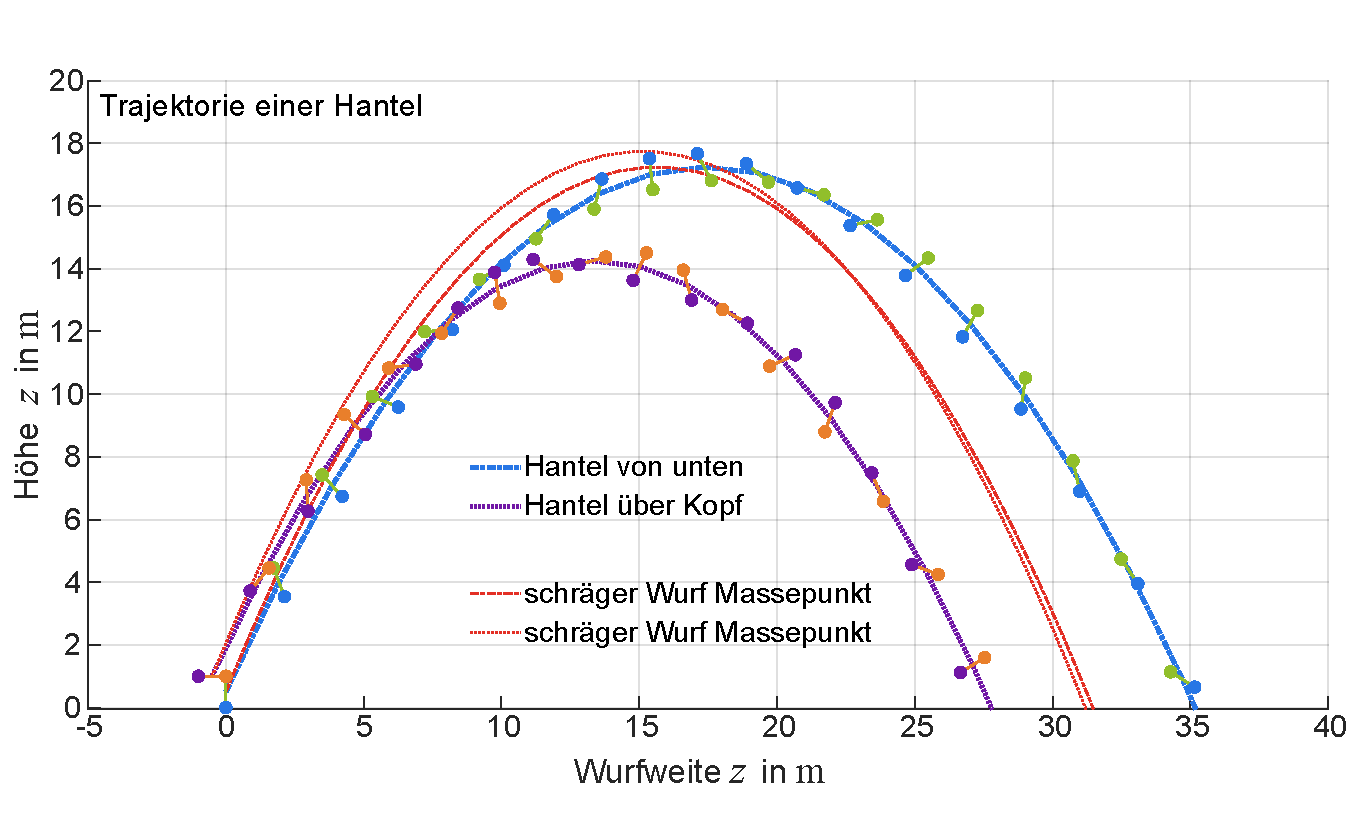
\includegraphics[width=\textwidth]{Hantelwurf02.pdf}
\caption[Trajektorien f�r eine geworfene Hantel.]{Trajektorien f�r eine geworfene Hantel und Vergleich mit dem schr�gen Wurf (ohne Ber�cksichtigung der Luftreibung).} 
\label{abb:bew_Hantelwurf02}
\end{figure}

\end {sol} 
%\href{PhysikUncut_Part1.pdf#prb:bew_Hantelwurf}{\textcolor{blue} {$\rightarrow$ zur \probref{bew_Hantelwurf}.}}\\
\textcolor{blue} {$\rightarrow$ zur} \probref{bew_Hantelwurf}.\\
\noindent\rule[1ex]{\textwidth}{0.5pt}  \newpage

%-----------------------------------------------------------------------------------------------------------

\hypertarget{lsg:bew_galaxies}{}
\begin{sol}{prob:bew_galaxies}\label{lsg:bew_galaxies}%�bung42
\textbf{Kontraktion von Galaxien} \\ \\
Drehimpulse und Rotationsenergie spielen eine gro�e Rolle in der Himmelsmechanik (Kapitel 3 im Teil 2 dieser Reihe), der Astrodynamik (Kapitel 4 im Teil 2)  und der Astrophysik. Die meisten Systeme in diesen Bereichen sind rotierende Systeme, so auch die Sterne in Galaxien, die sich auf elliptische Bahnen um ein Zentrum bewegen. Da auf einer Galaxie in guter N�herung das einwirkende Drehmoment gleich Null ist, muss der Drehimpuls einer Galaxie\index{Galaxie} konstant sein. \\
Betrachten wir die zeitliche Entwicklung einer Galaxie, so kann man zu Beginn von einer kugelf�rmigen homogenen Masseverteilung ausgehen, die einen konstanten Drehimpuls $L$ hat. Dann hat diese Kugel mit dem Tr�gheitsmoment $J = \frac{2}{5}m\,R^2$ die Rotationsenergie
\begin{align}
    T_\text{Rot} = \frac{1}{2}\,J\,\omega^2 = \frac{1}{2}\,J\,\lk\frac{L}{J}\rk^2 = \frac{5L^2}{4m\,R^2} \,. \label{eq:bew_Galaxien01}
\end{align}
Die Rotationsenergie nimmt also mit $R^2$ ab. Andererseits gibt es eine Gravitationswirkung zwischen den einzelnen Sternen (Massenelemente) der Galaxie, deren differentielle potentielle Energie, das ist die potentielle Energie eines differentiellen Massenelements ($\D m = 4\pi\,r^2\,\varrho\,\D r$ mit $\varrho$ als Massendichte der Galaxie) in Bezug auf alle anderen Massenelemente, folgenderma�en bestimmt werden kann:
\begin{align}
\begin{split}
    \D U_\text{G} &= -\frac{G}{r}\,m\,\D m = -\frac{G}{r}\,\lk \frac{4}{3}\pi\,r^3\,\varrho\rk\lk 4\pi\,r^2\,\varrho\,\D r\rk \\
    &= -\frac{G}{3}\,\lk 4\pi\,\varrho\rk^2\,r^4\,\D r \,. \label{eq:bew_Galaxien02}
\end{split}
\end{align}
Gleichung \eqref{eq:bew_Galaxien02} beschreibt die (differentielle) \emph{gravitative Selbstenergie}\index{Selbstenergie! der Gravitation}. Darunter versteht man die Energie, die frei wird, wenn sich die Masse eines als kugelf�rmigen homogenen Objekts mit dem Radius $r$ um $\D r$ zusammenzieht.\footnote{Bei einer Abnahme der gravitativen Selbstenergie m�ssen andere Formen der Energie anwachsen. I.A. wird es zu einer Zunahme der kinetischen Energie der Teilchen kommen, damit zu einer Erh�hung der Temperatur oder zur Abstrahlung von Energie in Form von elektromagnetischen oder Gravitationswellen.} \\
Man muss zur Berechnung der gesamten Selbstenergie die Beitr�ge der potentiellen Energie zwischen allen Bestandteilen des Systems (z.B. den Sternen = Massepunkte einer Galaxie) aufsummieren. Die Integration von \eqref{eq:bew_Galaxien02} ergibt dann:
\begin{align}
\begin{split}
    U_\text{G} = \int\limits_0^R\D\,U_\text{G}& = -\frac{G}{3}\,\lk 4\pi\varrho\rk^2\,\frac{R^5}{5} = -\frac{3}{5}\,\lk \frac{4}{3}\pi\,\varrho\,R^3\rk^2\,\frac{G}{R} = -\frac{3}{5}\,m^2\,\frac{G}{R}\,. \label{eq:bew_Galaxien03}
\end{split}
\end{align}
Wir setzen nun
\begin{align}
    E_\text{ges}\lk R\rk = T_\text{Rot} + U_\text{G} = \frac{5}{4}\,\frac{L^2}{m\,R^2} - \frac{3}{5}\,\frac{G\,m^2}{R} \, \label{eq:bew_Galaxien04}
\end{align}
und k�nnen dann $ E_\text{ges}\lk R\rk$ graphisch auftragen (\figref{bew_Galaxien01}). Man erkennt, dass es einen Radius 
\begin{align*}
    R_\text{end} = \frac{25\,L^2}{6\,G\,m^3}
\end{align*}
gibt, bei dem die Gesamtenergie minimal wird und den man �ber Extremwertberechnung leicht bestimmen kann. Umgekehrt kann man aus dem Wert f�r $R_\text{end}$ den Drehimpuls der Galaxie absch�tzen. Mit den Werten f�r die Andromeda-Galaxie\index{Andromeda-Galaxie}\footnote{Hinweis: Die Andromeda-Galaxie ist keine kugelf�rmige Galaxie, sondern eine Scheibengalaxie, zur Absch�tzung der Werte soll diese hier aber als kugelf�rmig angenommen werden.} $R_\text{end} = 10^5 \, \text{Lichtjahre}$ \bzw $m \approx \SI{2e42}{\kg}$ ergibt sich der Drehimpuls zu $L \approx \SI{1.8e67}{\J\second} $. 
Diese Werte wird die Galaxie im Gleichgewichtszustand annehmen, eine weitere Kontraktion auf Grund der Eigengravitation kann zumindest f�r eine kugelf�rmige Galaxie nicht mehr erfolgen. L�sst man die Forderung nach einer Kugelsymmetrie fallen, dann kann es durch uniaxiale Kontraktion parallel zur Rotationsachse zu einer weiteren Kontraktion der Galaxie kommen. So entstehen dann die scheibenf�rmigen Galaxien. Die Berechnung der entsprechenden Gleichgewichtszustandes erfolgt nach der gleichen Methode, die Integrale sind allerdings deutlich aufwendiger, da man zwei Koordinaten ($r,\vartheta$) \bzw ($r,z$) zu ber�cksichtigen hat. Wir werden solche Probleme im Rahmen der Potentialtheorie der Elektrodynamik behandeln. 
\begin{figure}[H]\centering
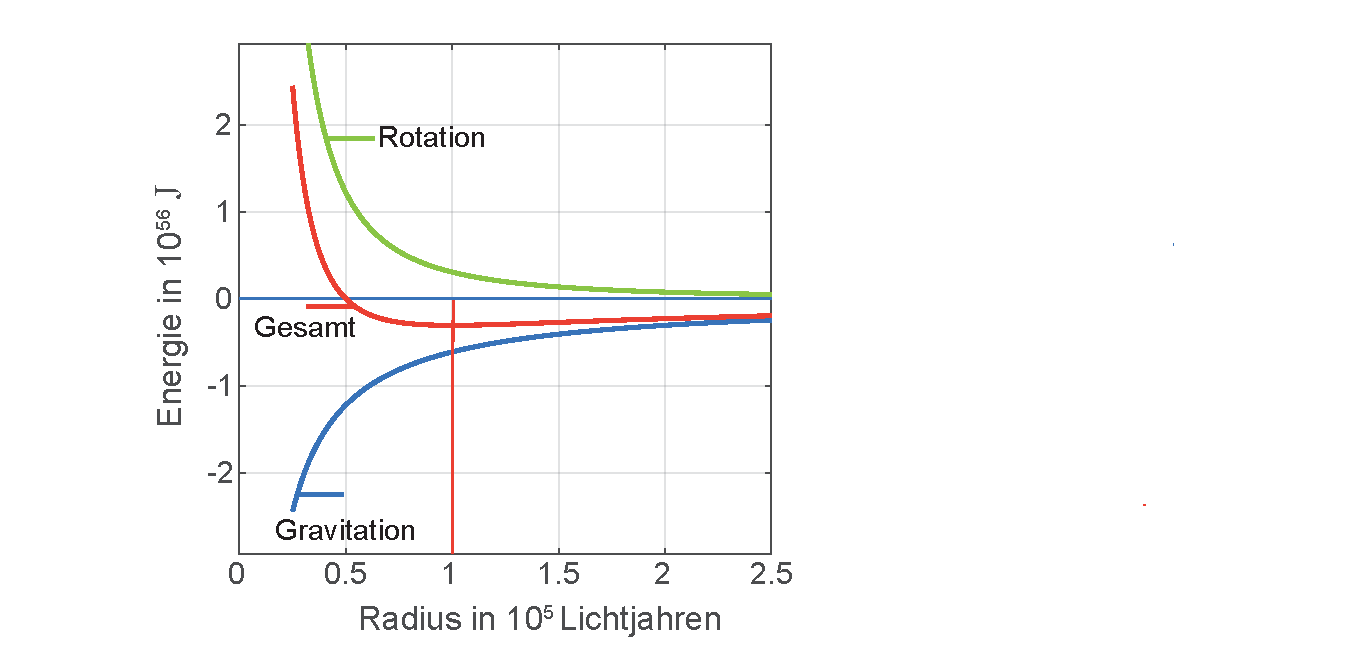
\includegraphics[width=\textwidth]{Galaxien01.pdf}
\caption{Energieverh�ltnisse bei einer rotierenden Galaxie.} 
\label{abb:bew_Galaxien01}
\end{figure}
\end{sol} 
%\href{PhysikUncut_Part1.pdf#prb:bew_galaxies}{\textcolor{blue} {$\rightarrow$ zur \probref{bew_galaxies}.}}\\
\textcolor{blue} {$\rightarrow$ zur} \probref{bew_galaxies}.\\
\noindent\rule[1ex]{\textwidth}{0.5pt}  \newpage


%-----------------------------------------------------------------------------------------------------------
\hypertarget{lsg:bew_Automobil}{}
\begin{sol}{prob:bew_Automobil}\label{lsg:bew_Automobil} %�bung43
\textbf{Automobilbeschleunigung} \\


\begin{figure}[H]\centering
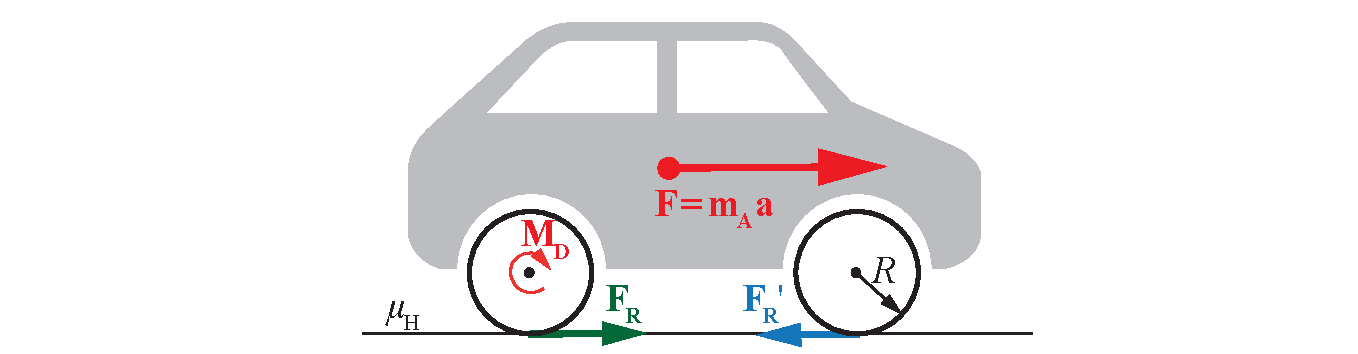
\includegraphics[width=\textwidth]{Automobil01.pdf}
\caption[Drehmomente und Kr�fte am beschleunigten Automobil (Hinterradantrieb).]{Drehmomente und Kr�fte am beschleunigten Automobil (Hinterradantrieb).} 
\label{abb:bew_lsgauto01}
\end{figure}

\begin{itemize}
	\item \textit{Maximale Beschleunigung, die ein Auto mit Hinterradantrieb entwickeln kann}\\ \\
Wir betrachten \figref{bew_lsgauto01}, die Hinterradachse ist als starr angenommen. 
Das gesamte Fahrzeug inklusive R�der habe die Masse $m_\text{A}$, ein einzelnes Rad $m_\text{R}$, der Durchmesser des Rades betrage $2R$.\\
Um das Fahrzeug anzutreiben, wirke auf die Hinterradachse das Drehmmoment $\vec{M}_\text{D}$, welches das einzelne Rad (Tr�gheitsmoment $J_\text{R}$) nach vorn treibt und beschleunigt. 
\begin{align}
\begin{split}
    \vec{M}_\text{D} + \vec{M}_\text{D,R} &= \vec{M}_\text{D,ges} = \dot{\vec{L}}_\text{R} ~~\leftrightarrow~~ \frac{M_\text{D}}{2} - F_\text{R}\,R = J_\text{R}\,\dot{\omega}_\text{R} \,. \label{eq:bew_lsgauto01}
\end{split}
\end{align}
Hierbei haben wir angenommen, dass ebenfalls ein Drehmoment $\vec{M}_\text{D,R}$ wirkt, welches durch eine statische Reibungskraft $F_\text{R}$ zustande kommt. Dieses 
ist dem Drehmoment der angetriebenen Hinterachse entgegengerichtet, was bedeutet, dass die Reibungskraft $F_\text{R,H}$ nach vorn gerichtet sein muss. Die Kraft  $F_\text{R}$ verhindert, dass das Rad anf�ngt nach hinten zu gleiten und bewirkt damit, dass der Punkt $P$ momentan fest und die Rollbedingung $v=R\,\omega$ erf�llt ist. \\
Wenn wir einen Haftreibungskoeffizienten $\mu_\text{H}$ annehmen, dann ist die maximale wirkende Reibungskraft $F_\text{R}$ bei angenommerner Gleichverteilung der Fahrzeugmasse auf alle R�der gegeben durch: 
\begin{align}
    F_\text{R} = F_\text{N}\,\mu_\text{H} = \frac{m_\text{A}}{4}\,g\,\mu_\text{H}\,. \label{eq:bew_lsgauto02}
\end{align}
Das gesamte Fahrzeug beschleunigt sich mit 
\begin{align}
    a = \frac{F_\text{ges}}{m_\text{A}}\,. \label{eq:bew_lsgauto02a}
\end{align}
F�r die beiden Vorderr�der, die nicht angetrieben sind, muss die dort wirkende Reibungskraft $F_\text{R}'$ nach hinten gerichtet sein, damit sich das Rad nach vorn dreht. Es gilt also:
\begin{align}
   \vec{M}_\text{D,R}' &= \dot{\vec{L}}_\text{R}~~\leftrightarrow~~ F_\text{R}'\,R = J_\text{R}\,\dot{\omega}_\text{R}\,.\label{eq:bew_lsgauto03}
\end{align}
Wir haben also die etwas \anf{verwirrende Situation}, dass um gleiche Drehrichtung der R�der zu erzeugen, bei gleichem Untergrund einmal die Reibungskraft in Bewegungsrichtung des Autos ($F_\text{R}$) und einmal entgegengesetzt ($F_\text{R}'$) zu dieser wirkt.  $F_\text{R}$ und $F_\text{R}'$ sind die einzigen am Auto angreifenden Kr�fte, die dieses nach vorn beschleunigen k�nnen (\bzw verz�gern k�nnen), also gilt: 
\begin{align}
    2F_\text{R} - 2F_\text{R}' = m_\text{A}\,a \,. \label{eq:bew_lsgauto04}
\end{align}
Wir haben somit drei Gleichungen f�r drei Unbekannte, $a$, $F_\text{R}$, $F_\text{R}'$. Gegeben sind das Drehmoment $M_\text{D}$, die Massen $m_\text{A}$, $m_\text{R}$ und der Radradius $R$. Wenn wir die R�der als Zylinder annehmen, erhalten wir mit $J_\text{R} = \frac{1}{2}\,m_\text{R}\,R^2$:
\begin{subequations}
\begin{align}
    a = \frac{R\,M_\text{D}}{4J_\text{R} + m_\text{A}\,R^2}  &= \frac{1}{R\,\lk 2m_\text{R}+m_\text{A}\rk}\,M_\text{D}\,, \label{eq:bew_lsgauto05a}\\
    F_\text{R} = \frac{\lk 2J_\text{R} + m_\text{A}\,R^2\rk\,M_\text{D}}{R\,\lk 4J_\text{R} + m_\text{A}\,R^2\rk} &= \frac{m_\text{A} + m_\text{R}}{2R\,\lk 2m_\text{R} + m_\text{A}\rk} \,M_\text{D} \,,\label{eq:bew_lsgauto05b}\\
    F_\text{R}' = \frac{J_\text{R}\,M_\text{D}}{R\,\lk 4J_\text{R}+m_\text{A}\,R^2\rk} &= \frac{m_\text{R}}{2R\,\lk 2m_\text{R}+m_\text{A}\rk}\,M_\text{D}\,. \label{eq:bew_lsgauto05c}
\end{align} \label{eq:bew_lsgauto05}
\end{subequations}

Die Frage ist nun, wie gro� die maximale Beschleunigung werden kann. Mit \eqref{eq:bew_lsgauto03} und \eqref{eq:bew_lsgauto05b} erhalten wir f�r $m_\text{A} \gg m_\text{R}$ n�herungsweise
\begin{align}
    F_\text{R} = \frac{M_\text{D}}{2\,R} ~~\text{\bzw}~~F_\text{R,max} =  \frac{m_\text{A}}{4}\,g\,\mu_\text{H}~~ \rightarrow ~~ F_\text{R} \leq F_\text{R,max} ~~\rightarrow~~M_\text{D} \leq \frac{m_\text{A}}{2}\,g\,R\,\mu_\text{H} \,. \label{eq:bew_lsgauto06}
\end{align}
Andererseits ist die Beschleunigung $a$ wiederum f�r $m_\text{A} \gg m_\text{R}$ n�herungsweise: 
\begin{align}
    a \approx \frac{M_\text{D}}{m_\text{A}\,R}\,,  \label{eq:bew_lsgauto07}
\end{align}
so dass aus \eqref{eq:bew_lsgauto06} und \eqref{eq:bew_lsgauto07} folgt:
\begin{align}
    a_\text{(max)} \leq \frac{\mu_\text{H}\,g}{2} \,. \label{eq:bew_lsgauto08}
\end{align}
Die maximale Beschleunigung wird also durch den Gleitreibungskoeffizienten $\mu_\text{H}$ bestimmt und kann bei typischen Werten von $\mu_\text{H} = \SI{0.5}{}\ldots\SI{0.7}{}$ nicht gr��er als $ a= \SI{2.5}{}\ldots\SI{3.7}{\metre\per\square \second}$ werden. Allerdings muss dazu auch das notwendige passende Drehmoment vorhanden sein, idealerweise durch \eqref{eq:bew_lsgauto05a} gegeben:
\begin{align*}
    M_\text{D} \approx 2R\,a\,m_\text{A} \approx \SI{600}{\newton\metre} \ldots \SI{750}{\newton\metre} \\
    \lk m_\text{A} = \SI{1.5}{\tonne}\,,\,R= \SI{0.3}{\metre}\rk ~~~~ \rightarrow ~~~~ 2R\,m_\text{A} \approx \SI{1500}{\kg\metre}
\end{align*}
Gr��ere Drehmomente bringen nichts, das Fahrzeug f�ngt an zu rutschen, bei kleineren Drehmomenten wird nicht die maximale Beschleunigung erreicht. Ebenso sieht man, dass gr��ere R�der (bei gleicher Masse) bei einem gegebenen Drehmoment eine geringere Beschleunigung erzeugen, andererseits ist bei gegebenen $\mu_\text{H}$ (damit maximal erreichbare Beschleunigung) bei gr��eren R�dern ein gr��eres Drehmoment nutzbar, was sich positiv auf das Zugverhalten (hier nicht untersucht) des Fahrzeugs auswirkt. \\
	\item \textit{Vorderantrieb/Allradantrieb} \\ \\
F�r einen Vorderantrieb gilt das Gesagte analog. Der Vorteil der starren Hinterachse beim Beschleunigungsverhalten resultiert daraus, dass \ia �ber die lenkbare Vorderachse nicht das gleiche Drehmoment erzeugt werden kann. F�r einen Allradantrieb ver�ndern sich \eqref{eq:bew_lsgauto04} und \eqref{eq:bew_lsgauto01} zu: 
\begin{align*}
%    4F_\text{R,A} &= m_\text{A}\,a   \\
    \frac{M_\text{D}}{4} - R\,F_\text{R,A} &= J_\text{R}\,\dot{\omega}_\text{R} = \frac{1}{2}\,m_\text{R}\,R^2\,\dot{\omega}_\text{R}\,,~~\dot{\omega}_\text{R} = \frac{a}{R}\,,~~
    \frac{M_\text{D}}{4} - \frac{m_\text{A}}{4}\,a\,R &= \frac{1}{2}\,m_\text{R}\,R\,a \\
%    M_\text{D} &= a\,\lk m_\text{A} + 2m_\text{R} \rk\,R  \\
    \rightarrow a &= \frac{M_\text{D}}{m_\text{A}\,R}
\end{align*}
Die maximale Reibungskraft ist wiederum
\begin{align*}
    F_\text{R,max} = \frac{m_\text{A}}{4}\,g\,\mu_\text{H}\,,
\end{align*}
woraus dann die maximale Beschleunigung im Allradantrieb sich zu 
\begin{align}
    a_\text{max} = \mu_\text{H} \, g \label{eq:bew_lsgauto09}
\end{align}
ergibt, also doppelt so gro� wie im Hinterradantrieb.\footnote{Die Gleichungen \eqref{eq:bew_lsgauto05} gelten mit entsprechenden Parametern v�llig analog f�r ein Fahrrad \bzw Motorrad.} \\
%In \mlbewref{Autobeschleunigung.m} haben wir verschiedene Parameters�tze f�r typische PKW durchgerechnet und auch den bisher vernachl�ssigten Effekt aus den Massen der R�der ber�cksichtigt (\figref{bew_lsgauto02}). 

\begin{figure}[H]\centering
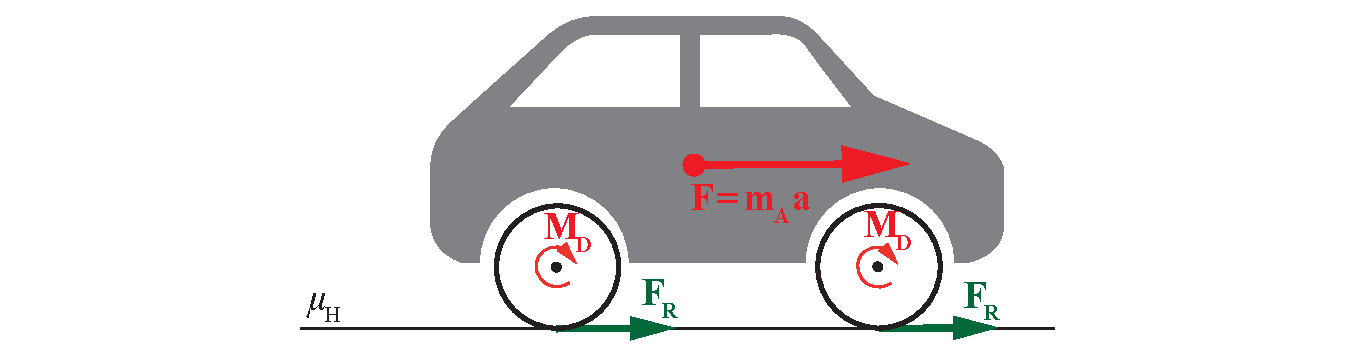
\includegraphics[width=\textwidth]{Automobil02.pdf}
\caption{Drehmomente und Kr�fte am beschleunigten Automobil (Allradantrieb).} 
\label{abb:bew_lsgauto02}
\end{figure}


%\begin{figure}[H]\centering
%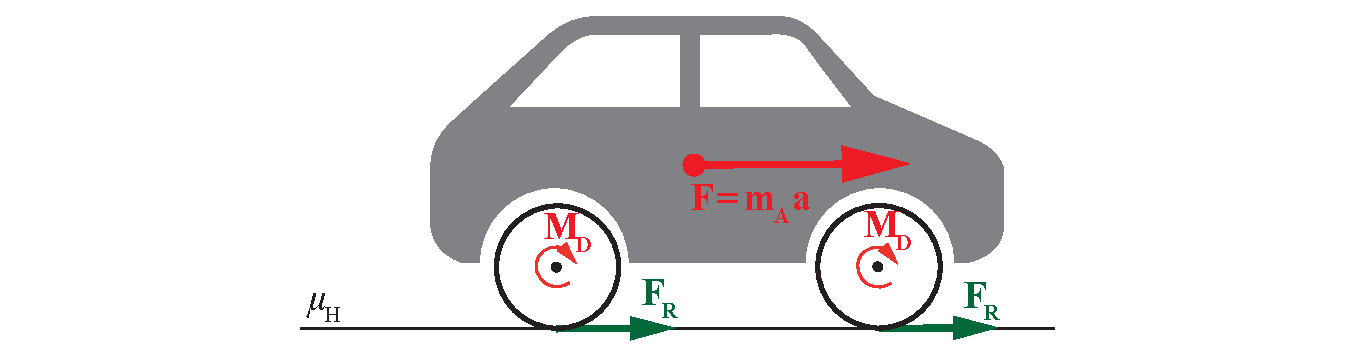
\includegraphics[width=\textwidth]{Automobil02.pdf}
%\caption{Beschleunigung und Drehmoment eines Automobils} 
%\label{abb:bew_lsgauto02}
%\end{figure}

	\item \textit{Energiebetrachtung} \\ \\
Zum Schluss wollen wir uns noch kurz der Energie zuwenden. Offensichtlich gewinnt das Fahrzeug bei einer Beschleunigung kinetische Energie. Die Frage ist, welche Kraft leistet eigentlich die Arbeit? Die einzige nach vorne wirkende Kraft ist ja $F_\text{R,H}$ (wir betrachten den Hinterradantrieb). Entsprechend der Definition der Arbeit gilt:
\begin{align*}
    W &= \int\limits_0^{s_\text{end}} \underbrace{2\lk F_\text{R} - F_\text{R}'\rk}_{\Delta F_\text{R}} \D s ~~~~ \text{mit} ~~~~ s_\text{end} = \frac{a}{2}\,t_\text{end}{}^2 ~~~~ \text{und} ~~~~ v_\text{end} = a\,t_\text{end} \\
    \frac{m_\text{A}\,v_\text{end}{}^2}{2} &= \underbrace{\Delta F_\text{R}\int\limits_0^{s_\text{end}}\D s}_{\substack{\text{\anf{Scheinarbeit}}}}  = \Delta F_\text{R}\,\frac{v_\text{end}{}^2}{2a} ~~~~ \text{mit} ~~~~  s_\text{end} = \frac{v_\text{end}{}^2}{2a}
\end{align*}
Das ist zun�chst etwas �berraschend, dass eine Reibungskraft Arbeit zu verleisten mag und eine Zunahme von kinetischer Energie erbringt. \\
Setzt man aber 
\begin{align}
    \Delta F_\text{R} = \frac{m_\text{A}}{R\,\lk 2m_\text{R} + m_\text{A}\rk}\,M_\text{D}
\end{align}
in die Gleichung f�r die Arbeit ein, so sieht man, dass die Arbeit vom Drehmoment \anf{geleistet} wird, und die Reibungskraft nur die Vermittlung von Rotationsenergie in Translationsenergie erm�glicht.
\end{itemize} 


\end{sol} 
%\href{PhysikUncut_Part1.pdf#prb:bew_Automobil}{\textcolor{blue} {$\rightarrow$ zur \probref{bew_Automobil}.}}\\
\textcolor{blue} {$\rightarrow$ zur} \probref{bew_Automobil}.\\
\noindent\rule[1ex]{\textwidth}{0.5pt}  \newpage

%-----------------------------------------------------------------------------------------
\hypertarget{lsg:bew_EulerWinkel}{}
\begin{sol}{prob:bew_EulerWinkel}\label{lsg:bew_EulerWinkel} %�bung44
\textbf{Euler-Winkel} \\ \\
Wir suchen die Winkelgeschwindigkeit $\vec{\omega}'$ im mitrotierenden
Koordinatensystem $\vec{\Sigma}'$. Dazu stellen wir zun�chst die
Rotationsmatrizen f�r die drei Euler-Winkel auf.
\begin{itemize}
\item Die erste Drehung erfolgt um die Achse $\veceZ$, die zum Laborsystem
  geh�rt, und der Rotationswinkel lautet $\varphi$. Die zugeh�rige
  Rotationsmatrix hat damit die Form
  \begin{equation*}
    \mathbb{R}_z(\varphi) = \mathbb{R}_\varphi = \begin{pmatrix} \cos\varphi & \sin\varphi & 0 \\
      -\sin\varphi & \cos\varphi & 0 \\ 0 & 0 & 1 \end{pmatrix} \; .
  \end{equation*}
\item Die zweite Drehung erfolgt mit dem Rotationswinkel $\vartheta$ um die
  Knotenlinie, die entlang der $x$-Koordinate des
  "`Zwischen-Koordinatensystems"' nach der ersten Drehung liegt. In diesem
  Koordinatensystem lautet die Rotationsmatrix daher
  \begin{equation}
    \mathbb{R}_{x'}(\vartheta) =  \mathbb{R}_\vartheta = \begin{pmatrix} 1 & 0 & 0 \\ 0 & \cos\vartheta
      & \sin\vartheta  \\ 0 & -\sin\vartheta & \cos\vartheta \end{pmatrix} \; .
  \end{equation}
\item Die letzte Drehung erfolgt mit dem Rotationswinkel $\psi$ um die
  $\vecpez$-Achse. Die Rotationsmatrix dazu hat im aktuellen Koordinatensystem
  die Gestalt
  \begin{equation*}
    \mathbb{R}_{z''}(\psi)  = \mathbb{R}_\psi = \begin{pmatrix} \cos\psi & \sin\psi & 0 \\
      -\sin\psi & \cos\psi & 0 \\ 0 & 0 & 1 \end{pmatrix} \; .
  \end{equation*}
\end{itemize}
  
Damit k�nnen wir nun die Komponenten der Winkelgeschwindigkeit bestimmen.
Die Beitr�ge der drei Euler-Winkel betrachten wir getrennt und arbeiten uns
dabei in umgekehrter Richtung der Rotationen mit den drei Euler-Winkeln vom
mitrotierten Koordinatensystem $\vec{\Sigma}'$ zum Laborsystem $\vec{\Sigma}$
vor.
\begin{itemize}
\item Der einfachste Beitrag ist tats�chlich die Rotation durch den Winkel
  $\psi$. Diesen berechnen wir zu
  \begin{equation*}
    \vec{\omega}'_\psi = \mathbb{R}_\psi \begin{pmatrix} 0 \\ 0 \\ \dot{\psi}
    \end{pmatrix} = \begin{pmatrix} \cos\psi & \sin\psi & 0 \\
      -\sin\psi & \cos\psi & 0 \\ 0 & 0 & 1 \end{pmatrix} \begin{pmatrix} 0
      \\ 0 \\ \dot{\psi} \end{pmatrix}
    = \begin{pmatrix} 0 \\ 0 \\ \dot{\psi} \end{pmatrix}
  \end{equation*}
  Tats�chlich h�tten wir uns die Transformation $\vec{M}_\psi$ sparen k�nnen.
  Sie beeinflusst das Ergebnis nicht, da eine Rotation ihre eigene Achse
  nicht �ndert. Bei den folgenden Anteilen wollen wir das gleich
  ber�cksichtigen und die eigene Rotationsachse nicht ansetzen.

\item �ndert sich der Winkel $\vartheta$ zeitlich, transformieren wir
  das in das mitrotierende System durch
  \begin{equation*}
    \vec{\omega}'_\vartheta = \mathbb{R}_\psi \mathbb{R}_\vartheta \begin{pmatrix}
      \dot{\vartheta} \\ 0 \\ 0 \end{pmatrix} = \mathbb{R}_\psi \begin{pmatrix}
      \dot{\vartheta} \\ 0 \\ 0 \end{pmatrix} 
    = \begin{pmatrix} \cos\psi & \sin\psi & 0 \\
      -\sin\psi & \cos\psi & 0 \\ 0 & 0 & 1 \end{pmatrix} \begin{pmatrix}
      \dot{\vartheta} \\ 0 \\ 0 \end{pmatrix} 
    = \begin{pmatrix} \cos\psi\,\dot{\vartheta} \\ -\sin\psi\,\dot{\vartheta}
      \\ 0 \end{pmatrix} \; .
  \end{equation*}
\item Schlie�lich betrachten wir noch die zeitliche �nderung von $\varphi$.
  Diese Rotation ist in $\vec{\Sigma}$ gegeben und muss durch alle drei
  Rotationsmatrizen nach $\vec{\Sigma}'$ transformiert werden, wobei
  $\mathbb{R}_\varphi$ selbstverst�ndlich wieder keine Auswirkung hat.
  \begin{multline*}
    \vec{\omega}'_\varphi = \mathbb{R}_\psi \mathbb{R}_\vartheta  \mathbb{R}_\varphi
    \begin{pmatrix} 0 \\ 0 \\ \dot{\varphi} \end{pmatrix}
    = \mathbb{R}_\psi \mathbb{R}_\vartheta \begin{pmatrix} 0 \\ 0 \\ \dot{\varphi}
    \end{pmatrix}
    = \begin{pmatrix} \cos\psi & \sin\psi & 0 \\
      -\sin\psi & \cos\psi & 0 \\ 0 & 0 & 1 \end{pmatrix}
    \begin{pmatrix} 1 & 0 & 0 \\ 0 & \cos\vartheta
      & \sin\vartheta  \\ 0 & -\sin\vartheta & \cos\vartheta \end{pmatrix}
    \begin{pmatrix} 0 \\ 0 \\ \dot{\varphi} \end{pmatrix} \\
    = \begin{pmatrix} \cos\psi & \sin\psi & 0 \\
      -\sin\psi & \cos\psi & 0 \\ 0 & 0 & 1 \end{pmatrix}
    \begin{pmatrix} 0 \\ \sin\vartheta\,\dot{\varphi} \\ \cos\vartheta\,
      \dot{\varphi} \end{pmatrix}
    = \begin{pmatrix} \sin\psi\,\sin\vartheta\,\dot{\varphi} \\
      \cos\psi\,\sin\vartheta\,\dot{\varphi}\\ \cos\vartheta\,
      \dot{\varphi} \end{pmatrix}
  \end{multline*}
\end{itemize}

Die gesamte Winkelgeschwindigkeit in $\vec{\Sigma}'$ ergibt sich aus der
Summe der drei Anteile,
\begin{equation*}
  \vec{\omega}' =  \vec{\omega}'_\varphi + \vec{\omega}'_\vartheta +
  \vec{\omega}'_\psi
  = \begin{pmatrix} \sin\psi\,\sin\vartheta\,\dot{\varphi} + \cos\psi\,
    \dot{\vartheta} \\    
    \cos\psi\,\sin\vartheta\,\dot{\varphi} -\sin\psi\,\dot{\vartheta} \\
    \cos\vartheta\, \dot{\varphi} + \dot{\psi} \end{pmatrix}
\end{equation*}
Dies Ergebnis entspricht gerade Gleichung \eqref{eq:bew_EulerWinkel} aus
Kapitel \ref{kap:bew_EulerWinkel}.

Wir geben noch die Herleitung der Euler-Gleichungen an:
Wir starten von \eqref{eq:bew_EulerGleichung01} und lassen der Einfachheit halber die Striche weg:
\begin{align*}
    \vec{\theta}\,\dot{\vec{\omega}} + \vec{\omega}  \times \vec{\theta}\,\vec{\omega} = \vec{M}
\end{align*}
mit
\begin{align*}
    \vec{\theta} = 
    \begin{pmatrix}
    \theta_{11} & 0 & 0 \\
    0 & \theta_{22} & 0 \\
    0 & 0 & \theta_{33}
    \end{pmatrix}
    =
    \begin{pmatrix}
        J_1 & 0 & 0 \\
        0 & J_2 & 0 \\
        0 & 0 & J_3
    \end{pmatrix}\,.
\end{align*}
Die Abbildung $\vec{\theta}\,\dot{\vec{\omega}}$ ist
\begin{align*}
    \vec{\theta}\,\dot{\vec{\omega}} &= 
    \begin{pmatrix}
    J_1\,\dot{\omega}_1 \\
    J_2\,\dot{\omega}_2 \\
    J_3\,\dot{\omega}_3
    \end{pmatrix} \,,\\
    \vec{\omega} \times \vec{\theta}\,\vec{\omega} &= 
    \begin{bmatrix}
        \vec{e}_1 & \vec{e}_2 & \vec{e}_3 \\
        \omega_1 & \omega_2 & \omega_3 \\
        J_1\,\omega_1 & J_2\,\omega_2 & J_3\,\omega_3
    \end{bmatrix} \\
    &= 
    \begin{pmatrix}
    J_3\,\omega_2\,\omega_3 - J_2\,\omega_2\,\omega_3 \\
    -\lk J_3\,\omega_1\,\omega_3 - J_1\,\omega_1\,\omega_3\rk \\
    J_2\,\omega_1\,\omega_2 - J_1\,\omega_1\,\omega_2
    \end{pmatrix} \,,
\end{align*}
\begin{align*}
    \rightarrow ~~~~ 
    \begin{pmatrix}
    J_1\,\dot{\omega_1} \\
    J_2\,\dot{\omega_2} \\
    J_3\,\dot{\omega_3}
    \end{pmatrix}
    +
    \begin{pmatrix}
    \lk J_3 - J_2\rk\,\omega_2\,\omega_3 \\
    \lk J_1 -J_3 \rk \,\omega_1\,\omega_3 \\
    \lk J_2-J_1\rk\,\omega_1\,\omega_2 
    \end{pmatrix}
    = 
    \begin{pmatrix}
    M_1\\
    M_2\\
    M_3
    \end{pmatrix}\,.
\end{align*}

\end{sol} 
%\href{PhysikUncut_Part1.pdf#prb:bew_EulerWinkel}{\textcolor{blue} {$\rightarrow$ zur \probref{bew_EulerWinkel}.}}\\
\textcolor{blue} {$\rightarrow$ zur} \probref{bew_EulerWinkel}.\\
\noindent\rule[1ex]{\textwidth}{0.5pt}  \newpage


%%%-----------------------------------------------------------------------------------------------------------
\hypertarget{lsg:bew_conPendel}{}
\begin{sol}{prob:bew_conPendel}\label{lsg:bew_conPendel} %�bung45
\textbf{Konisches Pendel}\\ \\

\begin{figure}
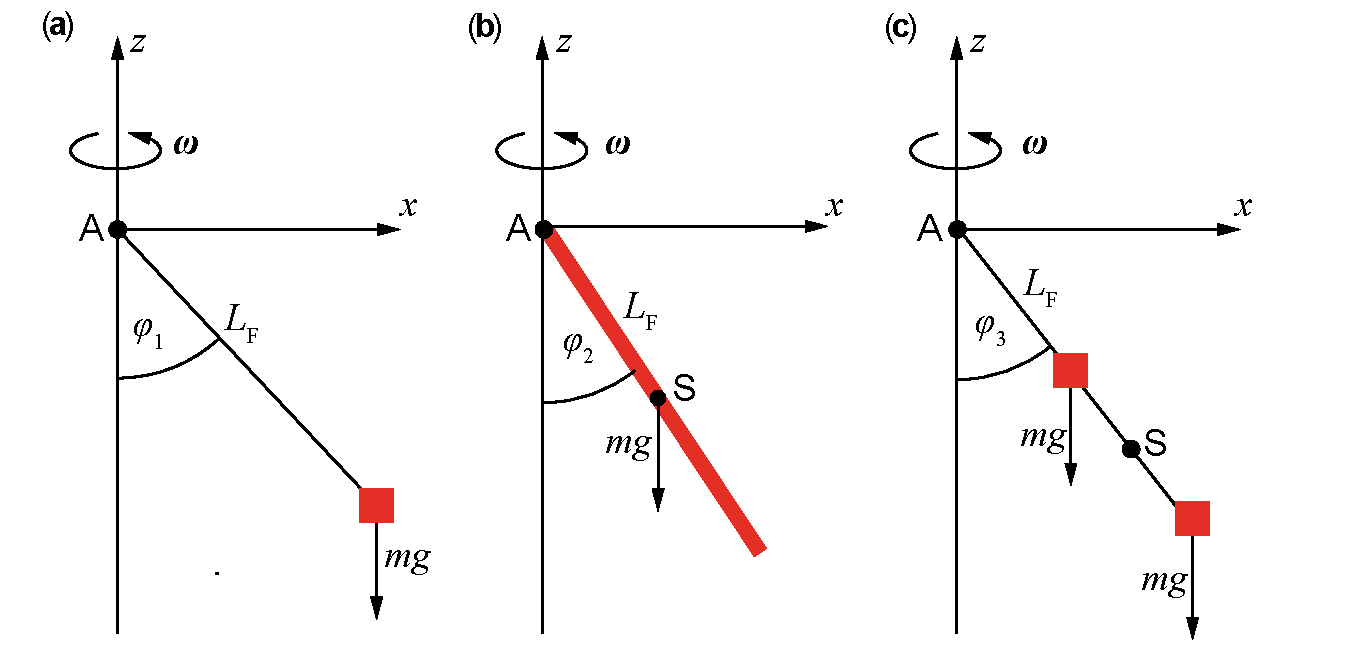
\includegraphics[width=\textwidth]{KonischesPendel01.pdf}
\caption[Verschiedene Formen des konischen Pendels]{Verschiedene Formen des konischen Pendels \fa Massepunkt  \fb Stange  \fc 2 Massepunkte auf einer masselosen Stange} 
\label{abb:bew_conPendel01a}
\end{figure}

\begin{enumerate}
    \item [a)] Konisches Pendel mit Massepunkt (\figref{bew_conPendel01a}a) \\
    
    Wir w�hlen den einfachen Weg der Newtonschen Mechanik und fordern das die Fadenkraft (Zwangskraft) sowohl die Zentrifugalkraft aufbringt, als auch die Gewichtskraft kompensiert. \\
    Dann gilt:
    \begin{align}
        \vec{F}_\text{F} = F_\text{T}\,
        \begin{pmatrix}
            \sin\varphi_1 \\
            0\\
            \cos\varphi_1
        \end{pmatrix}
        =
        \begin{pmatrix}
            m\,\omega^2\,r \\
            0\\
            m\,g
        \end{pmatrix} \,. \label{eq:bew_conPendel01}
    \end{align}
    Mit $L_\text{F}\,\sin\varphi_1 = r $ folgt daraus:
    \begin{align}
        \tan\varphi_1 &= \frac{\omega^2\,L_\text{F}\,\sin\varphi_1}{g} ~~~\rightarrow ~~~ \cos\varphi_1 = \frac{g}{L_\text{F}\,\omega^2}\,. \label{eq:bew_conPendel02}
    \end{align}
    Interessant ist, dass f�r $\omega^2\,L_\text{F} > g$ (also schnelle Drehung) der Kosinus reell wird und damit die Umlaufzeit von\\
		$T= 2\pi\sqrt{L_\text{F}\,\cos\varphi_1/g}$ \\
		hat. Dies entspricht der Umlaufzeit eines um $\cos\varphi_1$ verk�rzten Pendels der L�nge $L$.
    \item [b)] Konisches Pendel aus einer massiven Stange der L�nge $L_\text{F}$ (\figref{bew_conPendel01a}b) \\

    Hier k�nnen wir nicht so einfach die Newtonsche Mechanik anwenden, da die Stange ein ausgedehnter starrer K�rper ist und man sich �berlegen muss, wo die Kr�fte (\bzw Drehmomente) angreifen. Die Gewichtskraft ist gegeben durch $\vec{F}_\text{G} = -M\,g\,\vec{e}_\text{z}$ und greift im Schwerpunkt $S$ an, hat also bezogen auf $A$ das Drehmoment
  \begin{align}
        \vec{M}_\text{G} = \frac{L_\text{F}}{2}\,\sin\varphi_2\,m\,g\,\vec{e}_y \,. \label{eq:bew_conPendel03}
    \end{align}
    Die gesamte Zentrifugalkraft (im mitbewegten Koordinatensystem) zeigt immer in radialer Richtung und ergibt sich durch Integration �ber die differentiellen Massenelemente zu:
    \begin{align}
        F_z = \int\limits_0^{L_\text{F}} r\,\omega^2\,\D m = \int\limits_0^{L_\text{F}}s\,\sin\varphi_2\,\omega^2\,\frac{m}{L_\text{F}}\,\D s = \frac{1}{2}\,L_\text{F}\,\sin\varphi_2\,\omega^2\,m \,. \label{eq:bew_conPendel04}
    \end{align}
    Daraus folgt das Drehmoment:
    \begin{align}
        \vec{M}_\text{z} &= \int\limits_0^{L_\text{F}} s\,\cos\varphi_2\,\D F_z = \int\limits_0^{L_\text{F}} \cos\varphi_2\,\sin\varphi_2\,\omega^2\,\frac{m}{L_\text{F}}\,s^2\,\D s\,\vec{e}_y\nonumber \\
        &= \frac{1}{3}\,L_\text{F}{}^2\,\cos\varphi_2\,\sin\varphi_2\,\omega^2\,m\,\vec{e}_y = \underbrace{\frac{2}{3}\,L_\text{F}\,\cos\varphi_2}_{\substack{r_z}} \, \underbrace{\frac{1}{2}\,L_\text{F}\,\sin\varphi_2\,\omega^2\,m}_{\substack{F_z}}\,\vec{e}_y \label{eq:bew_conPendel05} \,. 
    \end{align}
    Die Drehmomente $\vec{M}_z$ und $\vec{M}_\text{G}$ m�ssen im station�ren Zustand gleich sein, woraus folgt:
    \begin{align}
        \frac{1}{2}\,\sin\varphi_2\,g &= \frac{1}{3}\,L_\text{F}\,\cos\varphi_2\,\sin\varphi_2\,\omega^2 ~~~ \rightarrow ~~~~ \cos\varphi_2 = \frac{3g}{2\,L_\text{F}\,\omega^2} \,. \label{eq:bew_conPendel06}
    \end{align}
    Wenn man wiederum f�r relativ gro�e Winkelgeschwindigkeiten $\omega^2\,L_\text{F} > \frac{3}{2}\,g$ die Umlaufzeit $T$ berechnet, findet man mit 
    \begin{align*}
        T = 2\pi\,\sqrt{\frac{2\cos\varphi_2}{3}\,\frac{L_\text{F}}{g}}
    \end{align*}
    die Schwingungsdauer eines um $\cos\varphi_2$ verk�rzten physikalischen (Stangen)Pendels. \\
	
\begin{figure}
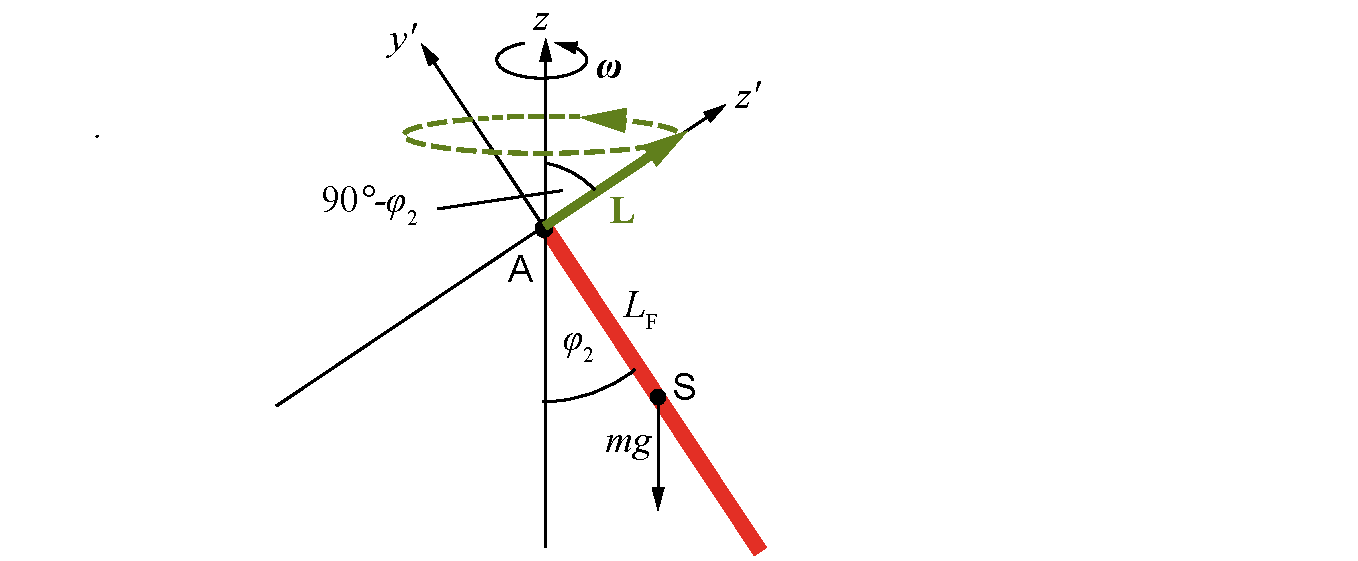
\includegraphics[width=\textwidth]{KonischesPendel02.pdf}
\caption{Zum konischen Pendel. Mitbewegtes Koordinatensystem} 
\label{abb:bew_conPendel02}
\end{figure}

    Man kann dieses Problem nat�rlich auch �ber die Euler-Gleichungen \bzw die Lagrange-Funktion (mit dem Euler-Winkel) l�sen. Wir �berlassen das dem Leser als zus�tzliche �bung, wollen hier aber kurz den Weg  skizzieren. Die Aufgabe besteht ja darin, die Tr�gheitsmomente und den Drehimpuls des Systems zu finden (bei als bekannt angenommenen $\omega$). Daraus bestimmt man �ber $\vec{M} = \D \vec{L}\\D t$ das Drehmoment.
    Wir wollen dazu ein k�rperfestes Koordinatensystem verwenden (\figref{bew_conPendel02}), das sich vom Inertialsystem dahingehend unterscheidet, dass die $y$-Achse in Richtung der Stabl�ngsachse zeigt und die $x$-Achse senkrecht dazu steht. 
    \begin{itemize}
        \item Die Haupttr�gheitsmomente sind $J_x = \frac{1}{3}\,m\,L_\text{F}{}^2,\,J_y = 0,\,J_z = \frac{1}{3}\,m\,L_\text{F}{}^2$
        \item Der Drehimpuls ergibt sich zu (wir lassen der Einfachheit halber die Striche weg, erinnern uns aber, dass wir im mitbewegten KOS sind): 
        \begin{align*}
				  \vec{L} = \begin{pmatrix}
            J_x\,\omega_x\\
            J_y\,\omega_y\\
            J_z\,\omega_z
        \end{pmatrix}~~  \text{mit}~~~\vec{\omega}  = \begin{pmatrix}
            \sin\varphi_2\\
            \cos\varphi_2\\
            0
        \end{pmatrix}~~
            \rightarrow ~~~ \vec{L} = \frac{1}{3}\,m\,L\text{F}{}^2\,\omega\,
            \begin{pmatrix}
                \sin\varphi_2\\
                0\\
                0
            \end{pmatrix}
        \end{align*}
        Wie man aus \figref{bew_conPendel02} sieht, beschreibt die Spitze des Drehimpulsvektors einen Kreis, dessen Umlaufgeschwindigkeit ist durch $\omega$ gegeben, sein Radius durch $|\vec{L}|\,\cos\varphi_2$. Damit gilt:\footnote{Analytisch kann man das auch �ber $\D \vec{L}/\D t = \vec{\omega} \times\vec{L}$ ableiten, woraus man auch die Richtung von $\D \vec{L}/\D t$ in Richtung von $-\vec{e}_z'$ erh�lt.} 
        \begin{align}
            \Big|\frac{\D \vec{L}}{\D t}\Big| = |\vec{L}|\,\cos\varphi\,\omega = \frac{1}{3}\,m\,L_\text{F}{}^2\,\omega\,\sin\varphi_2\,\cos\varphi_2 \,.
        \end{align}
        \item Das Drehmoment erhalten wir wieder �ber
        \begin{align*}
            \vec{M} &= \vec{r} \times \vec{F}_\text{G} = 
            \begin{pmatrix}
                0\\
                L/2\\
                0
            \end{pmatrix}
            \times 
            \begin{pmatrix}
                -m\,g\,\sin\varphi_2 \\
                -m\,g\,\cos\varphi_2 \\
                0
            \end{pmatrix} = -m\,g\,\frac{L}{2}\,\sin\varphi_2\,\vec{e}_z'
        \end{align*}
        \item Aus $\vec{M} = \D \vec{L}/\D t$ erhalten wir wie bereits in \eqref{eq:bew_conPendel06}
        \begin{align*}
            \cos\varphi_2 = \frac{3}{2}\,\frac{g}{L_\text{F}\,\omega^2}\,.
        \end{align*}
    \end{itemize}
		
    \item [c)] Konisches Massenpendel mit zwei Massepunkten auf einer masselosen Stange (\figref{bew_conPendel01a}c) \\
    
    Wir k�nnten analog wie im Fall b) vorgehen, wollen hier jedoch wieder einmal die St�rken des Lagrange-Formalismus demonstrieren. Wir finden unter Ber�cksichtigung  der Zwangsbedingung durch die starre Stange f�r den station�ren Zustand $\dot{\varphi} = \omega = \text{const}$:
    \begin{align}
        T&= \frac{1}{2}\,m\,L_\text{F}{}^2\,\sin^2\varphi_2\,\omega^2\,\lk \frac{1}{4} + \frac{4}{4}\rk = \frac{5}{8}\,m\,L_\text{F}{}^2\,\omega^2\,\sin^2\varphi_2 \nonumber\\
        U&= -m\,g\,\frac{L_\text{F}}{2}\,\cos\varphi_2 - m\,g\,L_\text{F}\,\cos\varphi_2 = -\frac{3}{2}\,m\,L_\text{F}\,\cos\varphi_2 \nonumber
    \end{align}
    \begin{align}
        \rightarrow ~~~~ \frac{\D}{\D t}\,\frac{\d \mathcal{L}}{\d \dot{\varphi}_2} - \frac{\d \mathcal{L}}{\d \varphi_2} &= 0 = \frac{5}{4}\,m\,L_\text{F}{}^2\,\omega^2\,\sin\varphi_2\,\cos\varphi_2 - \frac{3}{2}\,g\,m\,L_\text{F}\,\sin\varphi_2  \nonumber\\
        \rightarrow ~~~~ \cos\varphi_2 &= \frac{6}{5}\,\frac{g}{L_\text{F}\,\omega^2} \label{eq:bew_conPendel08} 
    \end{align}
\end{enumerate}

\end{sol} 
%\href{PhysikUncut_Part1.pdf#prb:bew_conPendel}{\textcolor{blue} {$\rightarrow$ zur \probref{bew_conPendel}.}}\\
\textcolor{blue} {$\rightarrow$ zur} \probref{bew_conPendel}.\\
\noindent\rule[1ex]{\textwidth}{0.5pt}  \newpage

%%%-----------------------------------------------------------------------------------------------------------
\hypertarget{lsg:bew_JoJoDynamik}{}
\begin{sol}{prob:bew_JoJoDynamik}\label{lsg:bew_JoJoDynamik}%�bung46
\textbf{Dynamik eines Jo-Jo} \\ \\
Wir wollen von \eqref{eq:bew_JoJo09} starten und uns noch einmal vergegenw�rtigen, dass 
\begin{align}
    z = z_\text{R} + z_\text{H}\,,~~~z_\text{R} = z-z_\text{H}\, \label{eq:bew_JoJo21}
\end{align}
gilt, worin $z$ die abgerollte Fadenl�nge darstellt, $z_\text{R}$ ist die Position des Jo-Jo \bzgl eines 0-Punktes im Raumkoordinatensystem und $z_\text{H}$ die Position der Hand relativ zum Ursprung dieses Koordinatensystems. Die f�r die Dynamik des Jo-Jos relevante Koordinate ist $z_\text{R}$. Eine Bewegung der Hand nach oben bedeutet, dann entsprechend der nach unten gew�hlten Richtung der $z$-Achse $z_\text{H}<0$, eine Bewegung der Hand nach unten folglich $z_\text{H}>0$. \\
Die Lagrange-Funktion ist dann gegeben durch 
\begin{align}
\begin{split}
    T &= \frac{m}{2}\,\lk \dot{z}_\text{R}\rk^2 + \frac{J}{2}\,\lk \frac{\dot{z}}{r\lk z\rk}\rk^2 \,, \\
    U &= -m\,g\,z_\text{R}\,, \\
    \rightarrow ~~~~ \mathcal{L} &= T-U = \frac{m}{2}\,\lk \dot{z}-\dot{z}_\text{H}\rk^2 + \frac{J}{2}\,\frac{\dot{z}^2}{r^2} + m\,g\,\lk z-z_\text{H}\rk \,.
\end{split} \label{eq:bew_JoJo22}
\end{align}
Man beachte, dass $z=z\lk t\rk$ und auch $z_\text{H} = z_\text{H}\lk t\rk$, wobei letztere eine unabh�ngige Funktion der Zeit ist. \\
Die Lagrange-Gleichung daraus lautet (etwas umgeformt):
\begin{align*}
    \frac{\D}{\D t}\,\lek \lk 1+\frac{J}{m\,r^2}\rk\,\dot{z}^2\rek = 2\,\lk g + \ddot{z}_\text{H}\rk\,\dot{z}\,.
\end{align*}
Das Integral daraus liefert:
\begin{align}
    \dot{z}^2 = \frac{2\,\lk g\,z + \int\limits_0^z \ddot{z}_\text{H}\,\lk z'\rk \,\D z' + C\rk}{1+J/m\,r^2}\,, \label{eq:bew_JoJo23}
\end{align}
worin $C$ eine durch die Anfangsbedingungen festgelegte Integrationskonstante ist. Hierbei haben wir angenommen, dass die Steuerfunktion $\ddot{z}_\text{H}\lk t\rk$ auch als Funktion der Koordinate $z$ geschrieben werden kann.\footnote{In der Realit�t wird genau das passieren, der Jo-Jo-Spieler \anf{steuert} das Jo-Jo je nach der L�nge des abgerollten Fenders und nicht nach der Zeit.} \\
Wir wollen jetzt annehmen, dass der wesentliche Energieverlust an kinetische Energie des Jo-Jos beim Umkippen passiert, wir schreiben den relativen Energieverlust als 
\begin{align}
    \Delta T = \frac{T_\downarrow-T_\uparrow }{T_\downarrow} = 1-\gamma^2 ~~~~ \text{mit} ~~~~ 0<\gamma<1 \,.  \label{eq:bew_JoJo24}
\end{align}
Hierin sind $T_\downarrow$ \bzw $T_\uparrow$ die kinetischen Energien vor bzw. nach Umschlagen des Jo-Jo. Gro�e $\gamma\approx 1$ bedeuten geringen Energieverlust und umgekehrt. Wir schreiben ferner $a_\text{H}\lk z\rk = \ddot{z}\lk z\rk$. Alternativ kann man nat�rlich auch einen zu $\dot{z}$ proportionale D�mpfung annehmen, worauf wir bei der Behandlung des Problems �ber die Lagrange-Gleichung zur�ck kommen werden. Zun�chst wollen wir aber \eqref{eq:bew_JoJo23} etwas auswerten. Man erkennt aus dieser Beziehung, dass die Terme
\begin{align*}
    \int\limits_0^L a_\text{H}^\downarrow\lk z'\rk\,\D z' ~~~~ \text{\bzw} ~~~~ \int\limits_L^0 a_\text{H}^\uparrow\lk z'\rk\,\D z\,
\end{align*}
nur dann zur Erh�hung der Geschwindigkeit $\dot{z}$ beitragen, wenn
\begin{align*}
    a_\text{H}^\downarrow > 0 ~~~~ \text{f�r} ~~~~ & 0\ldots z\ldots L\, \text{(zunehmende Fadenl�nge, Abwickeln)}\,, \\
    a_\text{H}^\uparrow < 0 ~~~~ \text{f�r} ~~~~ & L\ldots z\ldots 0\, \text{(abnehmende Fadenl�nge, Aufwickeln)}\,.
\end{align*}
Der Einfachheit wegen, nehmen wir konstante Beschleunigung der Hand in den beiden Phasen an, dann k�nnen wir den Energieerhaltungssatz (unter Ber�cksichtigung der D�mpfung im Umkehrpunkt) schreiben als:
\begin{align*}
    T \lk z= 0\rk = \Delta U\,\lk \gamma^2-1\rk + \gamma^2\,\underbrace{\int\limits_0^L F_\text{H}^\downarrow \D z + \int\limits_L^0 F_\text{H}^\uparrow \D z}_{W_\text{H}} \,.
\end{align*}
Dabei ist $W_\text{H}$ die durch die Bewegung der Hand geleistete Arbeit.
\begin{align}
    \rightarrow ~~~~ \dot{z}^2\lk 0\rk &= 2\,\frac{g\,L\,\lk \gamma^2-1\rk + \gamma^2\,\int\limits_0^L a_\text{H}^\downarrow\D z' - \int\limits a_\text{H}^\uparrow\D z'}{\lk 1 + J/m\,r^2 \rk} \label{eq:bew_JoJo25}  \\
    \rightarrow ~~~~ \dot{z}^2\lk 0\rk &= \frac{2}{\lk 1+J/m\,r^2\rk}\,\lek g\,L\,\lk \gamma^2-1\rk + \gamma^2\,\int\limits_0^L\lk a_\text{H}^\downarrow - a_\text{H}^\uparrow\rk \D z'\rek \label{eq:bew_JoJo26}
\end{align}
Wir nehmen an, dass die durch die Bewegung der Hand geleistete Arbeit gerade die Reibungsverluste kompensieren soll. Dar�ber hinaus soll die Beschleunigung in der Ab- und Aufrollphase jeweils konstant sein ($a_\text{H}^\uparrow$ = const \bzw $a_\text{H}^\downarrow$ = const)
\begin{align}
    \dot{z} \lk 0\rk^2 = 0 &= g\,L\,\lk \gamma^2-1\rk + \gamma^2\,\int\limits_0^L \lk a_\text{H}^\uparrow-a_\text{H}^\downarrow\rk \,\D z \nonumber \\
    \rightarrow ~~~~ g\,L\,\frac{1-\gamma^2}{\gamma^2} &= \int\limits_0^L \lk a_\text{H}^\uparrow-a_\text{H}^\downarrow\rk\,\D z \nonumber \\
    \text{Einfachster Fall:}\,~~~ a_\text{H}^\uparrow &= -a_\text{H}^\downarrow = \overline{a}_\text{H} > 0 \nonumber \\
    \rightarrow ~~~~ \overline{a}_\text{H} &= \frac{g}{2}\,\frac{\lk 1-\gamma^2\rk}{\gamma^2} \label{eq:bew_JoJo27}
\end{align}
Man erkennt, dass man f�r sehr starke D�mpfung ($\gamma\rightarrow 0$), sehr gro�e Beschleunigungen braucht. Deswegen beobachtet man bei einem Jo-Jo-Spieler eher ruckartige periodische Bewegungen der Hand. \\

\begin{figure}[H]\centering
  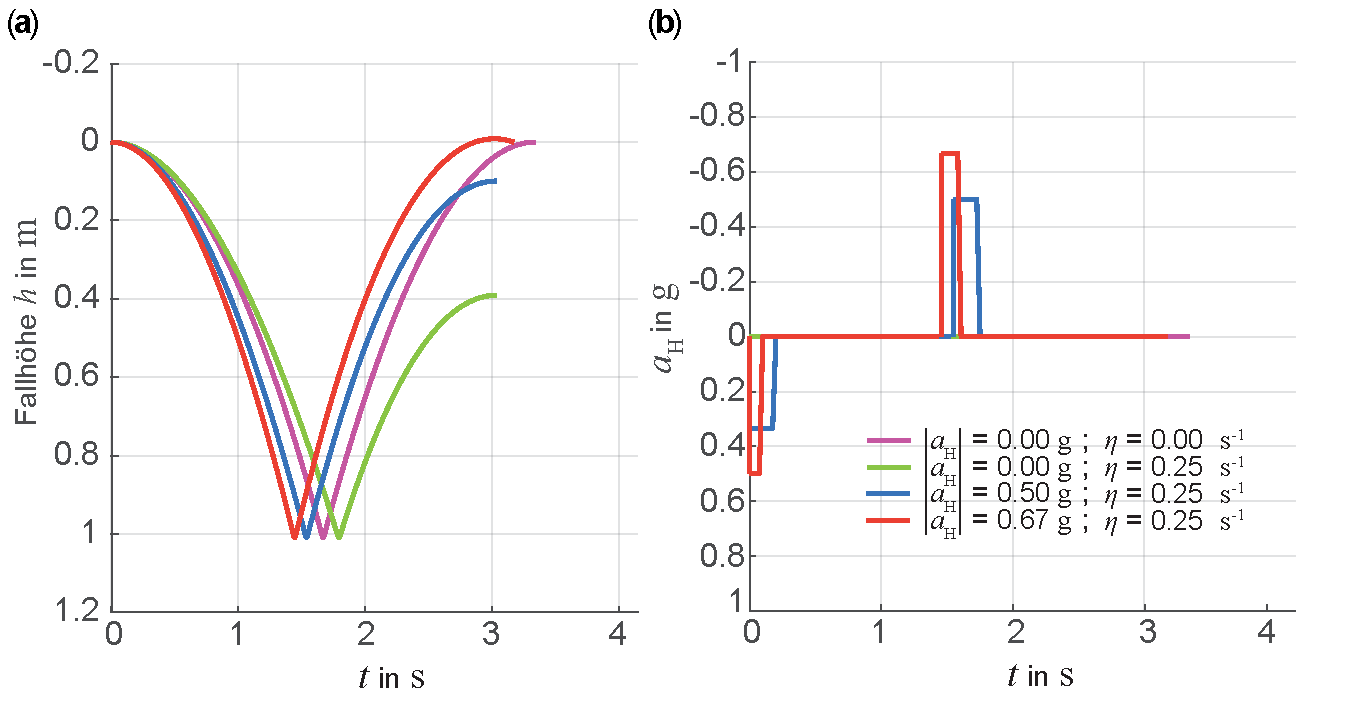
\includegraphics[width=\textwidth]{JoJo01.pdf}%
  \caption[Dynamik des gesteuerten Jo-Jos]{Dynamik des gesteuerten Jo-Jos f�r zwei verschiedene Anregungsfunktionen $a_\text{H}(t)$. \fa Fallh�he (Fadenl�nge) des Jo-Jo. \fb Zeitverlauf der Anregungsbeschleunigung der Hand. Parameter sind die Gr��e und Zeitdauer der Beschleunigung der Hand, sowie die Reibungskonstante $\eta$.}
  \label{abb:bew_JoJo01}
\end{figure}

In \mlbewref{JoJo02.m} wird die Dynamik des Jo-Jo nach Gleichung \eqref{eq:bew_JoJo23} f�r beliebige Anregungsfunktionen $a_\text{H}\lk z\rk$ und unterschiedliche D�mpfungen �ber die Lagrange-Gleichung numerisch untersucht, zwei Beispiele sind in \figref{bew_JoJo01} gezeigt.\\
Es sei darauf hingewiesen, dass aus \eqref{eq:bew_JoJo23} �ber
\begin{align*}
    \frac{\D z}{\D t} = \lek 2\,\frac{g\,z + \int\limits_0^z a_\text{H}\lk z'\rk\,\D z' + C}{\lk 1+J/m\,r^2 \lk z\rk\rk}\rek^\frac{1}{2}
\end{align*}
auch die Zeitentwicklung $t\lk z\rk$ \bzw als Umkehrfunktion die Kinematik $z\lk t\rk$ genommen werden kann:
\begin{align}
    t\lk z\rk = \frac{1}{2}\,\bigints\limits_0^z\lek \frac{\lk 1 + J/m\,r^2\lk z'\rk\rk}{g\,z' + \int\limits_0^{z'} a_\text{H}\lk z''\rk \,\D z'' + C}\rek^\frac{1}{2}\D z'\,. \label{eq:bew_JoJo28}
\end{align}
Gleichung \eqref{eq:bew_JoJo28} kann ebenfalls f�r bekannte $a_\text{H}\lk z\rk$ numerisch ausgewertet werden. Im Allgemeinen wird man jedoch von der Lagrange-Funktion \eqref{eq:bew_JoJo22} zur Lagrange-Gleichung �bergehen und diese numerisch l�sen, was wir in \mlbewref{JoJo02.m} realisiert haben. 


\begin{align}
\begin{split}
    \mathcal{L} &= \frac{m}{2}\,\lk \dot{z}-\dot{z}_\text{M}\rk^2 + \frac{J\lk z\rk}{2}\,\frac{\dot{z}^2}{r^2\lk z\rk} + m\,g\,\lk z-z_\text{M}\rk \\
    \frac{\d \mathcal{L}}{\d \dot{z}} &= m\,\lk \dot{z}-\dot{z}_\text{M}\rk + \frac{J\lk z\rk}{r^2\lk z\rk}\,\dot{z}\\
    \frac{\D}{\D t}\,\frac{\d \mathcal{L}}{\d \dot{z}} &= m\,\lk \ddot{z} - \ddot{z}_\text{M}\rk + \frac{J\lk z\rk}{r^2\lk z\rk}\,\ddot{z} + \dot{z}^2\,\lek \frac{\d J}{\d z}\,\frac{1}{r^2\lk z\rk} - 2\,\frac{J\lk z\rk}{r^3\lk z\rk}\,\frac{\d r}{\d z}\rek \\
    \frac{\mathcal{L}}{\d z} &= m\,g + \frac{\dot{z}^2}{2}\,\lek \frac{\d J}{\d z}\,\frac{1}{r^2\lk z\rk} - 2\,\frac{J\lk z\rk}{r^3\lk z\rk}\,\frac{\d r}{\d z}\rek
\end{split} \label{eq:bew_JoJo30}
\end{align}
\begin{align}
\begin{split}
    r\lk z\rk &= \sqrt{R_i{}^2 + d\cdot\lk L-z\rk} ~~~~\rightarrow ~~~~ \frac{\d r}{\d z} = -\frac{1}{2}\,\frac{d}{\sqrt{R_i{}^2 + d\cdot\lk L-z\rk }} \approx 0 \\
    J\lk z\rk &\approx J_0   ~~~~ \rightarrow ~~~~ \frac{\d J}{\d z} = 0
\end{split} \label{eq:bew_JoJo31}
\end{align}
\begin{align*}
    \frac{1}{m}\,\lek \frac{\D}{\D t}\,\frac{\d \mathcal{L}}{\d \dot{z}} - \frac{\d \mathcal{L}}{\d z}\rek = 0 \\
    \rightarrow ~~~~ \ddot{z} - \ddot{z}_\text{M} + \frac{J\lk z\rk}{m\,r^2\lk z\rk}\,\ddot{z} - \frac{J\lk z\rk}{m\,r^3\lk z\rk}\,\frac{\d r}{\d z}\,\dot{z}^2 -g=0 \\
    \rightarrow ~~~~ \ddot{z}\,\lk 1+\frac{J}{m\,r^2\lk z\rk}\rk = g + \ddot{z}_\text{M} + \frac{J}{m\,r^3}\,\frac{\d r}{\d z}\,\dot{z}^2
\end{align*}
Inklusive Reibung ergibt sich dann:
\begin{align}
    \ddot{z} &= \frac{1}{1+\frac{J}{m\,r^2\lk z\rk}}\,\lek g+ \ddot{z}_\text{M} + \frac{J}{m\,r^3}\,\frac{\d r}{\d z}\,\dot{z}^2\rek - \eta\,\dot{z}\,. \label{eq:bew_JoJo32}
\end{align}
F�r $J \approx \frac{m}{2}\,R_a{}^2$:
\begin{align*}
    \ddot{z} &= \frac{1}{1+\frac{R_a{}^2}{2\,r^2\lk z\rk}}\,\lek g+ \ddot{z}_\text{M} + \frac{R_a{}^2}{2\,r^3}\,\frac{\d r}{\d z}\,\dot{z}^2\rek - \eta\,\dot{z}\,.
\end{align*}
F�r $r^2\lk z\rk = R_i{}^2$, $\frac{\d r}{\d z}\approx 0$ (akademisches Jo-Jo):
\begin{align}
    \ddot{z} = \frac{1}{1+\frac{R_a{}^2}{2R_i{}^2}}\,\lek g + \ddot{z}_\text{M}\rek - \eta\,\dot{z} \,. \label{eq:bew_JoJo33}
\end{align}


\end{sol} 
%\href{PhysikUncut_Part1.pdf#prb:bew_JoJoDynamik}{\textcolor{blue} {$\rightarrow$ zur \probref{bew_JoJoDynamik}.}}\\
\textcolor{blue} {$\rightarrow$ zur} \probref{bew_JoJoDynamik}.\\
\noindent\rule[1ex]{\textwidth}{0.5pt}  \newpage

%%%-----------------------------------------------------------------------------------------------------------
%%%-----------------------------------------------------------------------------------------------------------

\newpage

\subsection{�bungen zur Mechanik der Kreisel}

\medskip

%-----------------------------------------------------------------------------------------------------------
\hypertarget{lsg:bew_freier_Kreisel}{}
\begin{sol}{prob:bew_freier_Kreisel}\label{lsg:bew_freier_Kreisel} %�bung47
\textbf{Rotation eines kr�ftefreien Kreisels} \\ \\
Die numerische Simulation des kr�ftefreien Kreisels ist in \mlbewref{KfKreiselDrehimpuls.m} hinterlegt.
Mit dieser wurden die beiden numerischen L�sungen aus
\figref{lsg_KfKreiselDrehimpuls1} und \figref{lsg_KfKreiselDrehimpuls2}
erstellt. In beiden Abbildungen sind F�lle dargestellt, bei denen, anders
als in Beispiel \ref{bsp:bew_unsymm_Kreisel}, die Rotation nicht um eine
der Haupttr�gheitsachsen erfolgt. Im Beispiel aus
\figref{lsg_KfKreiselDrehimpuls1} startet die Kreiselbewegung mit
$\vec{\omega}' = (\SI{1}{\per\s},\SI{0.8}{\per\s},0)$, also einer Drehung,
die signifikante Anteile von zwei Haupttr�gheitsachsen hat. Alle drei
Haupttr�gheitsachsen sind bereits in der Anfangssituation des Beispiels
aus \figref{lsg_KfKreiselDrehimpuls2} enthalten, in dem der anf�ngliche
Vektor $\vec{\omega}' = (\SI{0.3}{\per\s},\SI{0.8}{\per\s},\SI{0.4}{\per\s})$
lautet.

\begin{figure}[H]\centering
  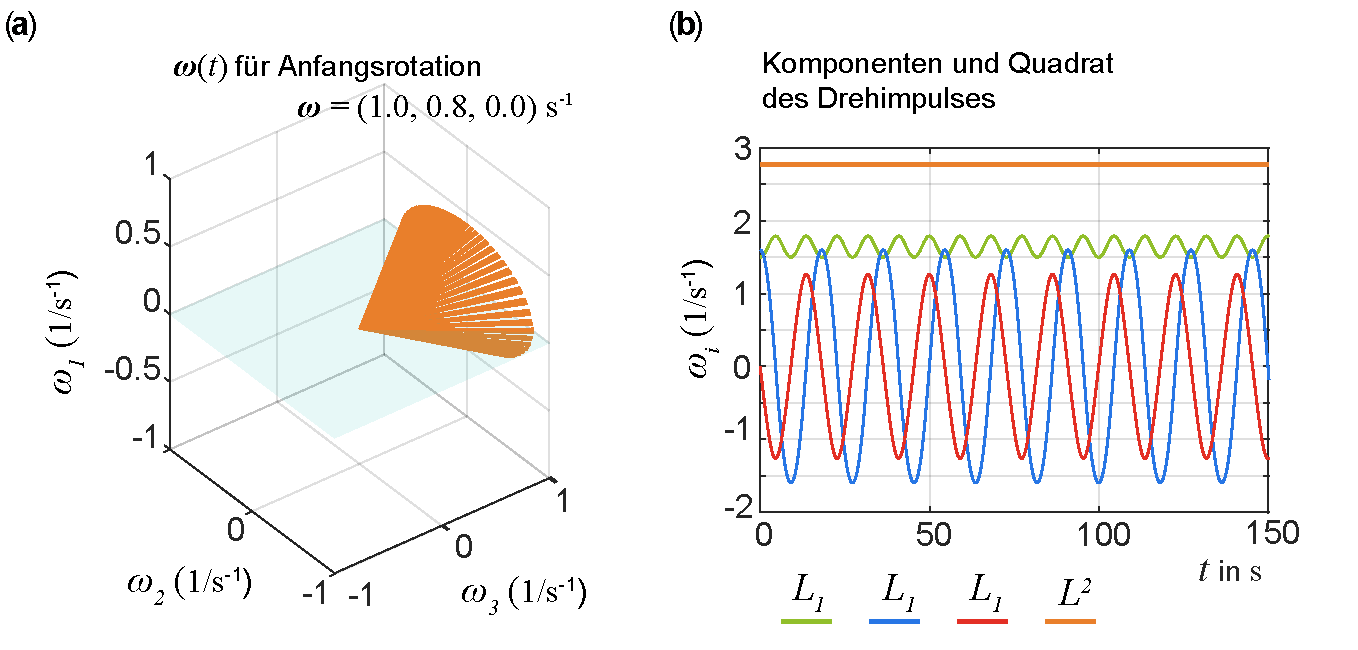
\includegraphics[width=\textwidth]{KfKreiselDrehimpuls1.pdf}%
  \caption[Drehachse sowie Komponenten und Quadrat des Drehimpulses]{Drehachse $\vec{\omega}'$ sowie Komponenten und Quadrat des
    Drehimpulses $\vec{L}'$ aus dem k�rperfesten System $\vec{\Sigma}'$
    f�r den Anfangswert $\vec{\omega}' = (\SI{1}{\per\s},\SI{0.8}{\per\s},0)$.}
  \label{abb:lsg_KfKreiselDrehimpuls1}
\end{figure}

\begin{figure}[H]\centering
  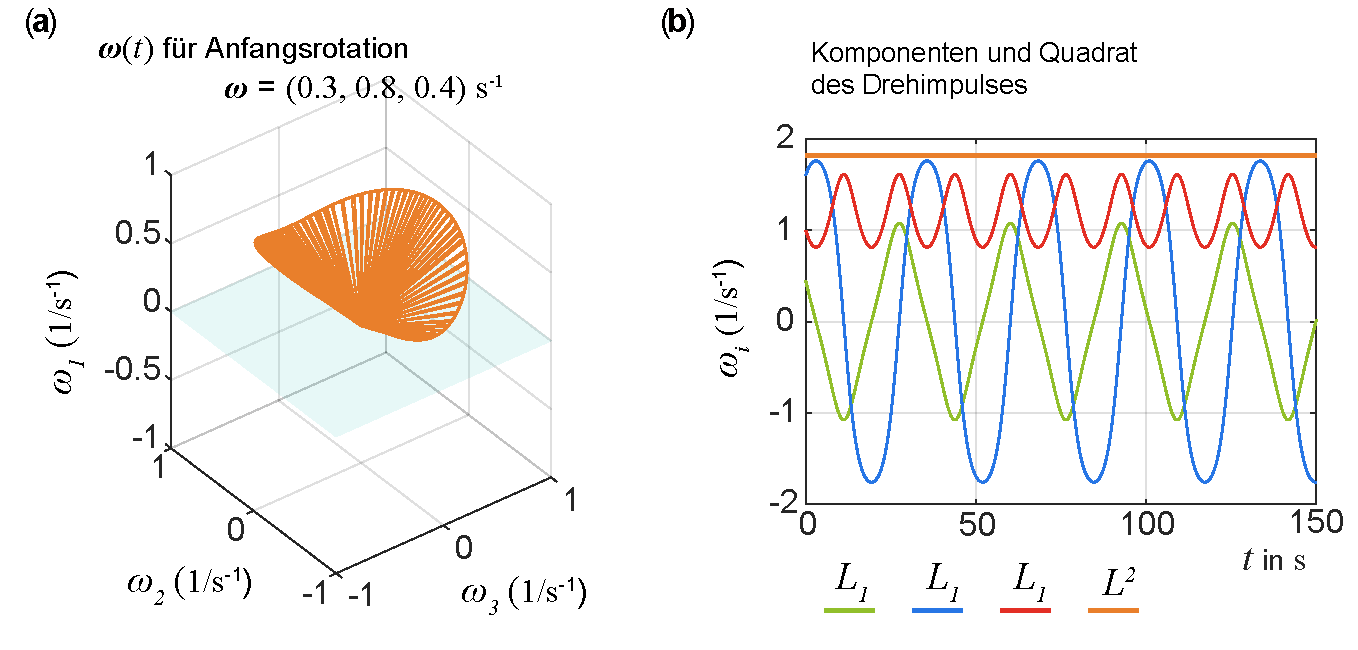
\includegraphics[width=\textwidth]{KfKreiselDrehimpuls2.pdf}%
  \caption[Drehachse sowie Komponenten und Quadrat des Drehimpulses]{Drehachse $\vec{\omega}'$ sowie Komponenten und Quadrat des
    Drehimpulses $\vec{L}'$ aus dem k�rperfesten System $\vec{\Sigma}'$
    f�r den Anfangswert $\vec{\omega}' = (\SI{0.3}{\per\s},\SI{0.8}{\per\s},
    \SI{0.4}{\per\s})$.}
  \label{abb:lsg_KfKreiselDrehimpuls2}
\end{figure}

In beiden Beispielen erkennt man, dass die Drehachse sich st�ndig �ndert und
dabei alle drei Haupttr�gheitsachsen einbezieht. Es sind also beides sicher
keine Spezialf�lle. Hier lohnt es, den Drehimpuls zu betrachten, was ebenfalls
in den Abbildungen dargestellt ist.

Die Komponenten der Drehimpulse sind in beiden F�llen nicht konstant, sondern
�ndern sich periodisch. Dies ist im k�rperfesten System $\vec{\Sigma}'$ zu
erwarten, denn der Drehimpuls ist im Raum unver�nderlich, was konstanten
Komponenten im Laborsystem $\vec{\Sigma}$ entspricht. Da das k�rperfeste
System relativ zu diesem seine Achsen periodisch verdreht, muss das f�r die
Projektion des Drehimpulses auf die Achsen von $\vec{\Sigma}'$ ebenfalls
gelten. Der Betrag des Drehimpulses (oder dessen Quadrat) ist jedoch
konstant. Dies wird numerisch in beiden dargestellten Beispielen best�tigt.

Die zeitliche Unabh�ngigkeit des Quadrats des Drehimpulses l�sst sich auch
leicht analytisch zeigen. Im k�rperfesten System $\vec{\Sigma}'$ gilt
\begin{equation*}
  \vec{L}' = \begin{pmatrix} J_1 \omega_1' \\ J_2 \omega_2' \\ J_3 \omega_3'
  \end{pmatrix}
\end{equation*}
und f�r die zeitliche Ableitung erh�lt man
\begin{equation*}
  \frac{\D}{\D t} \vec{L}'^2 = 2 \vec{L}'\cdot \frac{\D}{\D t}\vec{L}' =
  2 \begin{pmatrix} J_1 \omega_1' \\ J_2 \omega_2' \\ J_3 \omega_3' \end{pmatrix}
  \cdot
  \begin{pmatrix} J_1 \dot{\omega_1'} \\ J_2 \dot{\omega_2'} \\ J_3
    \dot{\omega_3'} \end{pmatrix} \; .
\end{equation*}
Hier setzt man nun die Kreiselgleichungen (Euler-Gleichungen) \eqref{eq:bew_Kreisel_frei} ein,
was auf
\begin{align}
  \frac{\D}{\D t} \vec{L}'^2 &= -2 
  \begin{pmatrix} J_1 \omega_1' \\ J_2 \omega_2' \\ J_3 \omega_3' \end{pmatrix}
  \cdot
  \begin{pmatrix} (J_3-J_2) \,\omega_2' \,\omega_3' \\ (J_1-J_3) \,\omega_1'
    \,\omega_3' \\ (J_2-J_1) \,\omega_1' \,\omega_2'\end{pmatrix} \nonumber \\
  &= -2 \left[ J_1 J_3 - J_1 J_2 + J_2 J_1 - J_2 J_3 + J_3 J_2 - J_3 J_1 \right ]
   \omega_1'  \omega_2'  \omega_3' = 0  \label{eq:bew_BetragDrehimpuls}
\end{align}
f�hrt. Die zeitliche �nderung des Betrags des Drehimpulses verschwindet also, der Betrag ist also konstant.

Die Stabilit�t oder Instabilit�t von Rotationen aus Beispiel
\ref{bsp:bew_unsymm_Kreisel} kann man sehr gut erkennen, wenn man f�r eine
kleine St�rung $\Delta\vec{\omega}(t)$ um eine station�re Rotation
$\vec{\omega}_0$ (d.h. eine Rotation mit $\dot{\vec{\omega}}_0 = 0$)
\begin{equation*}
  \vec{\omega}' = \vec{\omega}_0 + \Delta\vec{\omega}(t)
\end{equation*}
ansetzt. Eingesetzt in die Euler-Gleichungen \eqref{eq:bew_Kreisel_frei}
ergibt sich
\begin{align*}
  J_1 \Delta \dot{\omega}_1  &= -(J_3 - J_2)\, (\omega_{0,2}  + \Delta \omega_2 )
  (\omega_{0,3}  + \Delta \omega_3 ) \\
  J_2 \Delta \dot{\omega}_2  &= -(J_1 - J_3)\, (\omega_{0,1}  + \Delta \omega_1 )
  (\omega_{0,3}  + \Delta \omega_3 ) \\
  J_3 \Delta \dot{\omega}_3  &= -(J_2 - J_1)\, (\omega_{0,1}  + \Delta \omega_1 )
  (\omega_{0,2}  + \Delta \omega_2 ) \; .
\end{align*}
Ber�cksichtigt man, dass eine station�re Rotation $\vec{\omega}_0$ auch
erfordert, dass die quadratischen Termie mit $\omega_{0,i}\,\omega_{0,j}$ in dieser
Differentialgleichung verschwinden m�ssen, damit die Euler-Gleichungen
\eqref{eq:bew_Kreisel_frei} f�r $\omega_0$ erf�llt sind und linearisiert man
in der kleinen St�rung $\Delta\omega_i(t)$, dann verbleibt
\begin{align}
\begin{split}
  J_1 \Delta \dot{\omega}_1  &= -(J_3 - J_2) (\omega_{0,2}\,\Delta \omega_3
                               + \omega_{0,3}\,\Delta \omega_2 ) \\
  J_2 \Delta \dot{\omega}_2  &= -(J_1 - J_3) (\omega_{0,3}\,\Delta \omega_1
                               + \omega_{0,1}\, \Delta \omega_3 )\\
  J_3 \Delta \dot{\omega}_3  &= -(J_2 - J_1) (\omega_{0,1}\,\Delta \omega_2
                               + \omega_{0,2}\,\Delta \omega_1 )\; . 
\end{split} \label{eq:bew_EulerGlDeltas}
\end{align}

Der erste Fall aus Beispiel \ref{bsp:bew_unsymm_Kreisel} ist von der
Form
\begin{equation*}
  \vec{\omega_0} = \begin{pmatrix} \omega_{0,1} \\ 0 \\ 0 \end{pmatrix} \; .
\end{equation*}
Daf�r lauten die linearisierten Bewegungsgleichungen
\begin{align*}
  J_1 \Delta \dot{\omega}_1  &= 0 \\
  J_2 \Delta \dot{\omega}_2  &= -(J_1 - J_3)\, \omega_{0,1} \,\Delta \omega_3 \\
  J_3 \Delta \dot{\omega}_3  &= -(J_2 - J_1)\, \omega_{0,1} \,\Delta \omega_2 \,,
\end{align*}
an denen man erkennt, dass die St�rung nun die beiden bisher verschwindenden
Komponenten $\Delta \omega_2$ und $\Delta \omega_3$ koppelt. Man entkoppelt
die Differentialgleichungen, indem man \zb die zweite Gleichung ein
weiteres Mal ableitet und dann die dritte einsetzt. Man erh�lt
\begin{align}
\begin{split}
  J_2 \Delta \ddot{\omega}_2  &= -(J_1 - J_3)\, \omega_{0,1}\, \Delta
    \dot{\omega}_3 = \frac{(J_1 - J_3)(J_2 - J_1)}{J_3} \, \omega_{0,1}^2\,
  \Delta\omega_2 \\
  \intertext{\bzw}
  \Delta \ddot{\omega}_2  &= \frac{(J_1 - J_3)(J_2 - J_1)}{J_2 J_3} \,\omega_{0,1}^2\,
   \Delta\omega_2 \; .
\end{split} \label{eq:bew_EulerGlDeltas2}
\end{align}
Da in Beispiel \ref{bsp:bew_unsymm_Kreisel} $J_1 < J_2 < J_3$ gilt, ist der
Vorfaktor vor $\Delta \omega_2$ auf der rechten Seite der Gleichung negativ
(die erste Klammer im Z�hler ist negativ, die zweite positiv) und wir k�rzen
ihn mit
\begin{equation*}
  \frac{(J_1 - J_3)(J_2 - J_1)}{J_2 J_3} \omega_{0,1}^2 = - \Omega^2
\end{equation*}
ab. Die Differentialgleichung lautet also
\begin{equation*}
  \Delta \ddot{\omega}_2 = -\Omega^2 \Delta \omega_2
\end{equation*}
und hat die allgemeine L�sung
\begin{equation*}
  \Delta \omega_2(t) = A \cos(\Omega t) + B \sin(\Omega t) \; .
\end{equation*}
Dies ist eine stabile Oszillation um den station�ren Vektor $\vec{\omega}_0$.
Gleiches gilt f�r $\Delta \omega_3$ Die St�rung bleibt im Betrag immer gleich
gro�.\\

Der zweite Fall aus Beispiel \ref{bsp:bew_unsymm_Kreisel} geht von einer
station�ren Rotation
\begin{equation*}
  \vec{\omega_0} = \begin{pmatrix} 0 \\ \omega_{0,2} \\ 0 \end{pmatrix} \; .
\end{equation*}
aus und die linearisierten Bewegungsgleichungen \eqref{eq:bew_EulerGlDeltas} lauten damit
\begin{align*}
  J_1 \Delta \dot{\omega}_1  &= -(J_3 - J_2) \,\omega_{0,2} \,\Delta\omega_3 \\
  J_2 \Delta \dot{\omega}_2  &= 0 \\
  J_3 \Delta \dot{\omega}_3  &= -(J_2 - J_1) \,\omega_{0,3} \, \Delta \omega_1 \; ,
\end{align*}
Die Entkopplung der beiden von der St�rung gekoppelten Gleichungen
erreicht man z.B. mit
\begin{align}
\begin{split}
  J_1 \Delta \ddot{\omega}_1  &= -(J_3 - J_2) \omega_{0,2} \Delta
    \dot{\omega}_1 = \frac{(J_3 - J_2)(J_3 - J_1)}{J_2} \,\omega_{0,2}^2\,
  \Delta \omega_1 \\
  \intertext{\bzw}
  \Delta \ddot{\omega}_1  &= \frac{(J_3 - J_2)(J_3 - J_1)}{J_1 J_2} \, \omega_{0,2}^2\,
  \Delta \omega_1 
\end{split} \label{eq:bew_EulerGlDeltas1}
\end{align}
In diesem Fall sind beide Klammern im Z�hler positiv und damit ist es auch
der gesamte Vorfaktor. Wir bezeichnen ihn mit:
\begin{equation*}
  \frac{(J_3 - J_2)(J_3 - J_1)}{J_1 J_2} \omega_{0,2}^2 = \alpha^2 \,.
\end{equation*}
Die Differentialgleichung lautet also
\begin{equation*}
  \Delta \ddot{\omega}_1 = \alpha^2 \Delta \omega_1
\end{equation*}
und hat die allgemeine L�sung
\begin{equation*}
  \Delta \omega_1(t) = A \mathrm{e}^{\alpha t} + B \mathrm{e}^{\alpha t} \; .
\end{equation*}
Eine kleine St�rung steigt in diesem Fall also exponentiell an. Die Rotation
um die $\vecpeY$-Achse ist also instabil. Das gilt schon aufgrund
der L�sung f�r $\Delta \omega_1(t)$, jedoch findet man gleiches f�r die
zweite Komponente $\Delta \omega_3(t)$ der gekoppelten Differentialgleichungen \eqref{eq:bew_EulerGlDeltas1}.\\

Eine weitere Simulationsrechnung f�r einen kr�ftefreien Kreisel ist in \mlbewref{KfSymmKreiselSimul.m} hinterlegt.
Sie stellt die Bewegung der Figurenachse als auch des Polkegels und des Rastpolkegels dar.

\end{sol} 
%\href{PhysikUncut_Part1.pdf#prb:bew_freier_Kreisel}{\textcolor{blue} {$\rightarrow$ zur \probref{bew_freier_Kreisel}.}}\\
\textcolor{blue} {$\rightarrow$ zur} \probref{bew_freier_Kreisel}.\\
\noindent\rule[1ex]{\textwidth}{0.5pt}  \newpage

%-----------------------------------------------------------------------------------------------------------
\hypertarget{lsg:bew_Polbewegung}{}
\begin{sol}{prob:bew_Polbewegung}\label{lsg:bew_Polbewegung} %�bung48
\textbf{Polbewegung der Erde} \\ \\
Die in der Aufgabe behandelte Polbewegung ist die Folge der Tatsache, dass die Erde 
\begin{enumerate}   [1)]
	\item keine Kugel ist, sondern ein um $0.3\%$ abgeplatteter Rotationsellipsoid,
	\item kein komplett starrer K�rper ist, sondern eine gewisse Elastizit�t aufweist.
	\item die Erdoberfl�che jahreszeitliche Effekte und kleinere Deformationen zeigt,
	\item im Erdinneren langsame Massenverschiebungen stattfinden.
\end{enumerate}
Die Symmetrieachse der Erde (eine ihrer Hauptr�gheitsachsen) f�llt aus den genannten Gr�nden nicht genau mit ihrer Drehachse zusammen. Letztere geht durch den Schwerpunkt des Erdk�rpers. Darum \glqq taumelt\grqq{} der Erdk�rper ein wenig bez�glich seiner eigenen Drehachse, was sich in �nderungen der geographischen Koordinaten eines ortsfesten Beobachters bemerkbar macht. Wir wissen aus Kap. \ref{kap:bew_Kreisel_kraeftefrei}, dass ein solches Taumeln nur  dann stabil ist, wenn die Drehung (n�herungsweise) um die K�rperachse mit dem gr��ten oder dem kleinsten Tr�gheitsmoment stattfindet. Das ist aber genau hier der Fall. Die Abweichung zwischen Symmetrie- und Drehachse bleibt daher begrenzt und die Symmetrieachse vollf�hrt etwa einmal im Jahr eine Nutationsbewegung um die Drehachse, deren Periode wir berechnen wollen. Wir ber�cksichtigen dabei zun�chst nur den ersten der o.g. vier Effekte und betrachten die Erde als symmetrischen Kreisel.\\
Aus der Euler-Gleichung \eqref{eq:bew_EulerGleichung02} folgt dann sofort mit $\vec{M} = 0$ und $J_1 = J_2 =J_A$ und $J_3 = J_Z > J_A$:
\begin{align}
\begin{split}
    J_A\,\dot{\omega}_1{}' &= \lk J_A-J_Z\rk \,\omega_2{}'\,\omega_3{}'\,, \\
    J_A\,\dot{\omega}_2{}' &= \lk J_A-J_Z\rk \,\omega_1{}'\,\omega_3{}'\,, \\
     \dot{\omega}_3{}' &= 0 ~~~~ \rightarrow ~~~~ \omega_3{}' = \con \,.
\end{split} \label{eq:bew_Polbew01}
\end{align}
Wir addieren die erste und zweite Gleichung mit $q = \omega_1{}' + \im\,\omega_2{}'$ und erhalten
\begin{align}
    J_A\,\dot{q} = -\im\lk J_A-J_Z\rk \,q\,\omega_3{}'\,.  \label{eq:bew_Polbew02}
\end{align}
Die Abplattung der Erde wird i.A. definiert als 
\begin{align}
    \gamma = \frac{J_Z -J_A}{J_A} \approx \frac{1}{300}\,, \label{eq:bew_Polbew03}
\end{align}
so dass wir schreiben k�nnen:
\begin{align}
    \dot{q} = \im\,\gamma\,\omega_3{}'\,q\,.  \label{eq:bew_Polbew04}
\end{align}
Das ist einfach zu integrieren und ergibt
\begin{align}
    q = q_0\,\e^{\im\,\gamma\,\omega_3{}'\,t}\,. \label{eq:bew_Polbew05}
\end{align}
\eqref{eq:bew_Polbew05} beschreibt die Rotation der Projektion des Vektors $\vec{\omega}$ auf die �quatorebene.\footnote{Wir erinnern uns, dass wir �ber \eqref{eq:bew_Polbew02} definiert hatten.} \\Offensichtlich ist die Winkelgeschwindigkeit dieser Rotation um die Figurenachse $\vecpez$ konstant ($=\gamma\,\omega_3{}'$) und die Bewegung ist die im Kapitel \ref{kap:bew_Kreisel_kraeftefrei} hergeleitete Nutation. \\
Die Nutationsperiode ist dann 
\begin{align*}
    T_N = \frac{2\pi}{\gamma\,\omega_3{}'} &= \killA{2\pi}\,300\,\frac{86126}{\killA{2\pi}}\,\SI{}{\second}\,\frac{\text{d}}{\SI{86400}{\second}} \approx 299\,\text{d}\,.
\end{align*}

Wir erhalten also eine Nutationsperiode (Euler-Periode) von etwa 300 Tagen (bei einer Amplitude von \ca 6--10 m).
Es gibt noch die weiteren sich �berlagernden Effekte, die vor allem aus der plastischen Verformung des Erdinneren resultieren. Daher setzt sich die Gesamtperiode  aus den verschiedenen Komponenten zusammen und hat eher eine Periodendauer von 415 bis 433 Tagen (Chandlersche Periode). Die Schwankung der Periodendauer h�ngt mit jahreszeitlichen Effekten zusammen (Laubfall und Vegetation, Vereisung, Plattentektonik usw.). Aus dem Unterschied zwischen Chandler- und Euler-Periode kann die Starrheit des Erdk�rpers abgesch�tzt werden.\\

\end{sol} 
%\href{PhysikUncut_Part1.pdf#prb:bew_Polbewegung}{\textcolor{blue} {$\rightarrow$ zur \probref{bew_Polbewegung}.}}\\
\textcolor{blue} {$\rightarrow$ zur} \probref{bew_Polbewegung}.\\
\noindent\rule[1ex]{\textwidth}{0.5pt}  \newpage


%-----------------------------------------------------------------------------------------
\hypertarget{lsg:bew_schwerer_Kreisel}{}
\begin{sol}{prob:bew_schwerer_Kreisel}\label{lsg:bew_schwerer_Kreisel} %�bung49
\textbf{Rotation eines schweren symmetrischen Kreisels} \\ \\
Die numerische Simulation des schweren symmetrischen Kreisels ist in
\mlbewref{SchwererKreiselSim.m} implementiert.
Das Programm l�st die Bewegungsgleichungen \eqref{eq:bew_Lagrange_starrerK4c},
und \eqref{eq:bew_Lagrange_starrerK4a} aus Kapitel
\ref{kap:bew_SchwererSymmKr}.

Zus�tzlich soll die Bewegung der Figurenachse $\vec{F}$ dargestellt werden.
Diese erh�lt man durch die Transformation des Vektors $\vecpeZ$ in das
raumfeste Koordinatensystem. Dies geschieht durch die Drehung mit
den drei Eulerwinkeln,
\begin{multline*}
  \vec{fA} = \vec{M}_\psi \vec{M}_\vartheta  \vec{M}_\varphi
  \begin{pmatrix} 0 \\ 0 \\ 1 \end{pmatrix}
  = \vec{M}_\psi \vec{M}_\vartheta \begin{pmatrix} 0 \\ 0 \\ 1 \end{pmatrix}
  = \begin{pmatrix} \cos\psi & \sin\psi & 0 \\
    -\sin\psi & \cos\psi & 0 \\ 0 & 0 & 1 \end{pmatrix}
  \begin{pmatrix} 1 & 0 & 0 \\ 0 & \cos\vartheta
    & \sin\vartheta  \\ 0 & -\sin\vartheta & \cos\vartheta \end{pmatrix}
  \begin{pmatrix} 0 \\ 0 \\ 1 \end{pmatrix} \\
  = \begin{pmatrix} \cos\psi & \sin\psi & 0 \\
    -\sin\psi & \cos\psi & 0 \\ 0 & 0 & 1 \end{pmatrix}
  \begin{pmatrix} 0 \\ \sin\vartheta \\ \cos\vartheta \end{pmatrix}
  = \begin{pmatrix} \sin\psi\,\sin\vartheta \\
    \cos\psi\,\sin\vartheta\\ \cos\vartheta\, \end{pmatrix} \; .
\end{multline*}

Die allgemeine Bewegung ist eine �berlagerung aus
Nutation und Pr�zession und f�hrt zu einem komplexen Zeitverlauf der Ausrichtung
der Figurenachse im Raum. Die Nickbewegung der Nutation ist sehr klar
im Verlauf des Euler-Winkels $\vartheta$ zu erkennen. Sie �bertr�gt sich
zus�tzlich auf die Winkel $\varphi$ und $\psi$.

Den Fall mit Nutation erkennt man in 
\figref{bew_SchwererKreiselFigurenachse2}. F�r diesen Fall muss die Energie des Kreisels dem Minimum des effektiven Potentials entsprechen (siehe Kap. \ref{kap:bew_SchwererSymmKr_O_Nutation}).


\begin{figure}
  \centering
  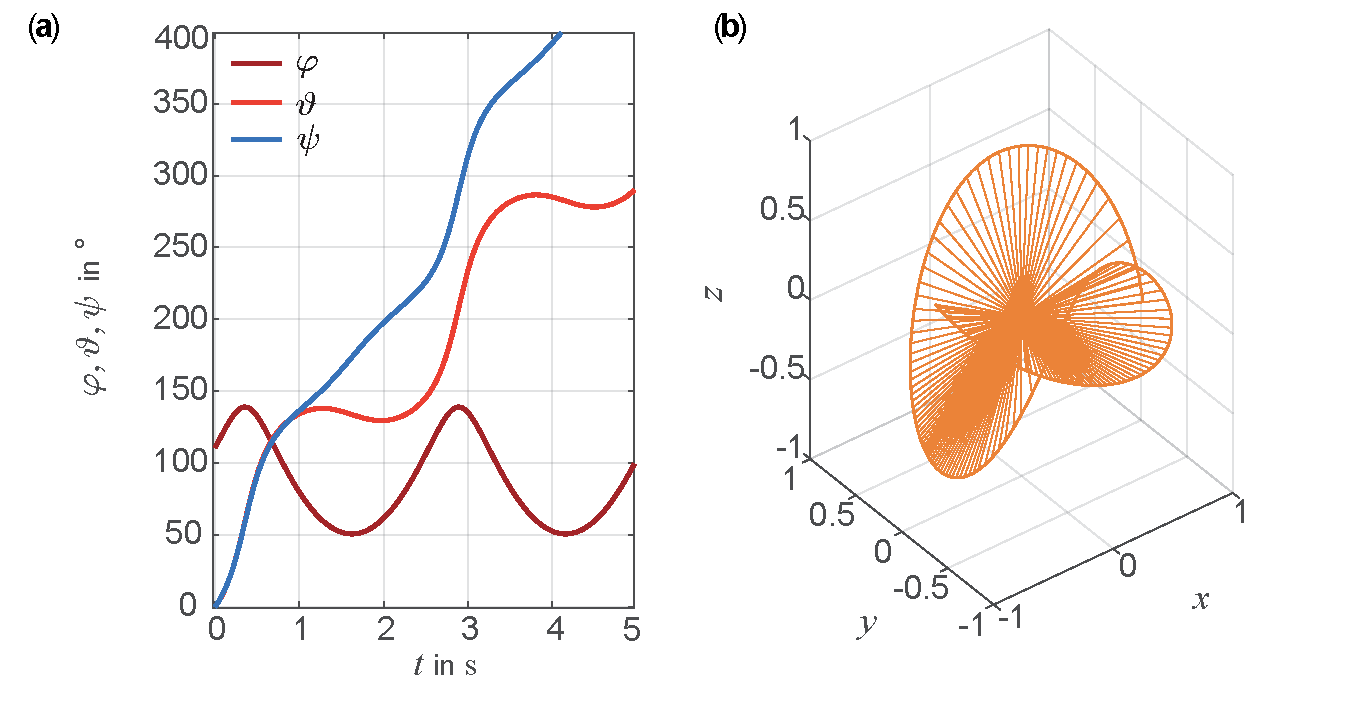
\includegraphics[width=\textwidth]{SchwererKreiselFAchse1.pdf}%
  \caption[Bewegung der Figurenachse eines schweren Kreisels mit Nutation]
  {Bewegung der Figurenachse eines schweren Kreisels im allgemeinen Fall mit
    Nutation. Die �berlagerte Bewegung ist komplex.}
  \label{abb:bew_SchwererKreiselFigurenachse1}
\end{figure}

Ein Fall ohne Nutation ist in Abbildung
\figref{bew_SchwererKreiselFigurenachse1} dargestellt. Die Figurenachse
bewegt sich auf einen Kreis parallel zum Boden. Hier liegt eine reine
Pr�zession vor.

\begin{figure}
  \centering
  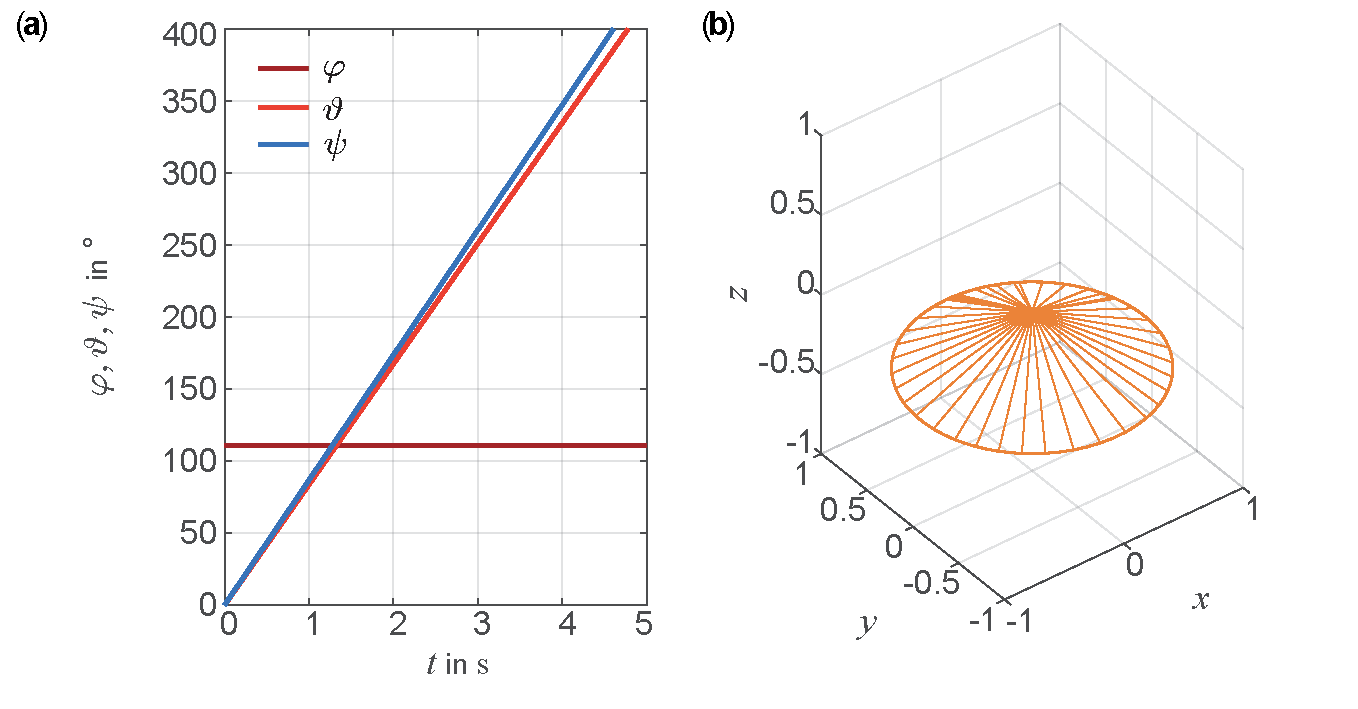
\includegraphics[width=\textwidth]{SchwererKreiselFAchse2.pdf}%
  \caption[Bewegung der Figurenachse eines schweren Kreisels ohne Nutation]
  {Bewegung der Figurenachse eines schweren Kreisels ohne Nutation. Es liegt
    eine reine Pr�zession vor, die an der Bewegung der Figurenachse auf einem
    Kreis parallel zum Boden zu erkennen ist.}
  \label{abb:bew_SchwererKreiselFigurenachse2}
\end{figure}

Zur anschaulichen Erkl�rung der Pr�zession eines Spielzeugkreisels �ber die wirkenden Kr�fte.\\

Am einfachsten kann man dies erkl�ren, wenn man sich in die Position des mitbewegten, \dh mit pr�zessierenden Beobachters auf die Kreiselachse "`setzt"'.
Wir m�ssen nat�rlich dann im mitbewegten System neben der Schwerkraft auch die Scheinkr�fte und insbesondere die Corioliskraft ber�cksichtigen.

\end{sol} 
%\href{PhysikUncut_Part1.pdf#prb:bew_schwerer_Kreisel}{\textcolor{blue} {$\rightarrow$ zur \probref{bew_schwerer_Kreisel}.}}\\
\textcolor{blue} {$\rightarrow$ zur} \probref{bew_schwerer_Kreisel}.\\
\noindent\rule[1ex]{\textwidth}{0.5pt}  \newpage


%-----------------------------------------------------------------------------------------------------------
\hypertarget{lsg:bew_unwucht}{}
\begin{sol}{prob:bew_unwucht}\label{lsg:bew_unwucht} %�bung50
\textbf{Auswuchten von R�dern und anderen rotierenden K�rpern}\\
\begin{figure}
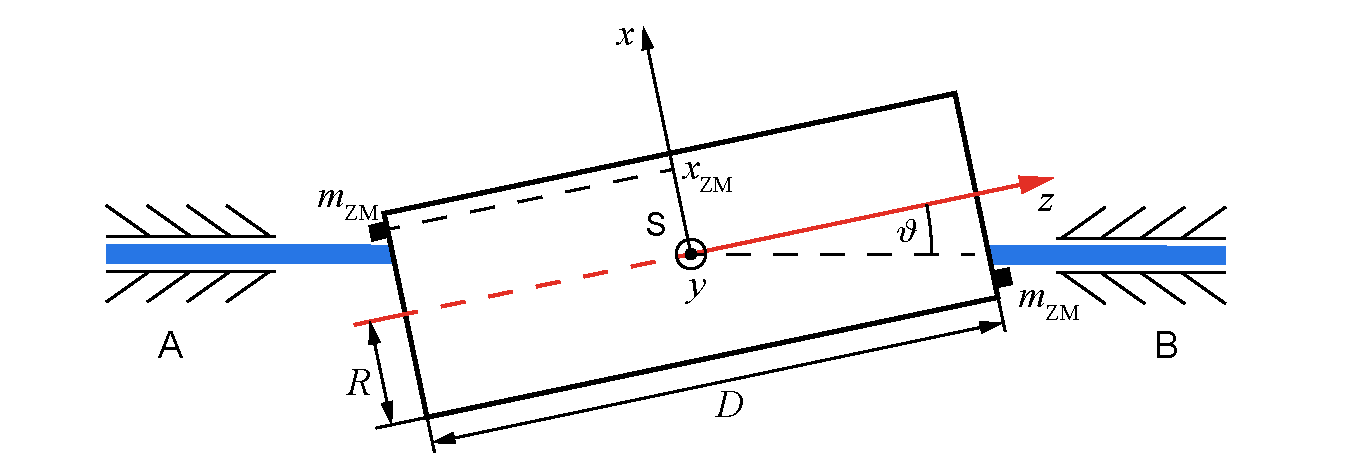
\includegraphics[width=\textwidth]{Unwucht02.pdf}
\caption[Auswuchten von dynamischen Unwuchten] {Auswuchten von dynamischen Unwuchten durch Anbringen vo9n Zusatzmassen} 
\label{abb:bew_unwucht02}
\end{figure}

Eine Unwucht, \zb bei einem Reifen liegt vor, wenn die Rotationsachse nicht einer seiner Haupttr�gheitsachse entspricht. Solche Unwuchten f�hren zu Vibrationen und belasten daher die Lager, die die Rotationsachse aufnehmen. Dies f�hrt zu einem entsprechend Verschlei�. Man versucht, Unwuchten durch geeignete Gegengewichte zu kompensieren. (\figref{bew_unwucht02}).
\begin{enumerate}
    % a)
    \item [a)]
    Wir berechnen zun�chst die auf die Lager wirkenden Kr�fte. Wir nehmen dabei der Einfachheit halber an, dass der Schwerpunkt auf der Rotationsachse liegt, die Haupttr�gheitsachse aber um einen Winkel $\vartheta$ gegen die Rotationsachse verkippt ist. Nach \figref{bew_unwucht02} ergeben sich dann aus Schwerpunktsatz \bzw Drehimpulssatz:
    \begin{align}
        F_\text{A} &= -F_\text{B}  \nonumber \\
        M_\text{U}' &= F_\text{A}\,L - F_\text{B}\,L = \dot{L}_\text{U}' = \frac{J_3-J_1}{2}\,\omega^2\,\sin\lk 2\vartheta\rk \nonumber \\
				\rightarrow ~~ F_\text{A} &= -F_\text{B}  = \frac{\omega^2}{2L}\,\frac{J_3-J_1}{2}\,\sin\lk 2\vartheta\rk \,. \label{eq:bew_unwucht03}
    \end{align}
\begin{nebenrechnung}

Zur Ableitung von \eqref{eq:bew_unwucht03} betrachte man einen symmetrischen Kreisel, der um die z-Achse zur Pr�zession mit einem festen Winkel $\vartheta$ und konstanter Frequenz $\omega_P$ gezwungen wird. Wir schreiben die Euler-Gleichungen Beachtung von (\figref{bew_unwucht03}) wie folgt:
    \begin{align*}
        \dot{\varphi} &= \omega_P = \text{const}\,, ~~~~ \dot{\psi} = \omega_K\,, ~~~~ \dot{\vartheta} = 0\,, ~~~~ \vec{\omega}_P + \vec{\omega_K} = \vec{\omega}'\,, \\
        \vec{\omega}' &= 
				\begin{pmatrix}
        \omega_1{}'\\
        \omega_2{}'\\
        \omega_3{}'
        \end{pmatrix}
        = 
        \begin{pmatrix}
        \omega_\text{P}\,\sin\vartheta\,\sin\psi \\
        \omega_\text{P}\,\sin\vartheta\,\cos\psi \\
        \omega_\text{P}\,\cos\vartheta + \omega_\text{K}
        \end{pmatrix}\,, \\ \\
        \dot{\vec{\omega}}' &=
				\begin{pmatrix}
        \dot{\omega}_1{}'\\
        \dot{\omega}_2{}'\\
        \dot{\omega}_3{}'
        \end{pmatrix}
        =
        \begin{pmatrix}
        \omega_\text{P}\,\omega_\text{K}\,\cos\psi\,\sin\vartheta \\
        -\omega_\text{P}\,\omega_\text{K}\,\sin\psi\,\sin\vartheta \\
        0
        \end{pmatrix}\,.
    \end{align*}
 \end{nebenrechnung}
    % b)
    \item [b)]
    Wir wollen nun den Reifen auswuchten. Dazu bringen wir kleine Massen (ZM steht f�r Zusatzmassen) so an, dass die neue Haupttr�gheitsachse mit der Drehachse �berein stimmt (\figref{bew_unwucht02}). Wir nehmen gleiche Massen links (L) und rechts (R) an, also $m_\text{R} = m_\text{L} = m_\text{ZM}$
    \begin{align}
    \begin{split}
        \dot{\vec{L}}'_\text{ZM} + \dot{\vec{L}}'_\text{U} &= 0 \,,\\
        \dot{\vec{L}}'_\text{ZM}= -\dot{\vec{L}}'_\text{U} &= -\vec{M}'_\text{U} = -\frac{J_3-J_1}{2}\,\omega^2\,\sin\lk 2\vartheta\rk\,
        \begin{pmatrix}
        0\\
        1\\
        0
        \end{pmatrix}\,,
    \end{split}  \label{eq:bew_unwucht04}
    \end{align}
    da das Drehmoment in negative $\vecpey$ Richtung zeigt. Folglich m�ssen die beiden Ausgleichsmassen in der Ebene liegen, die von $\vecpex$ und $\vecpez$ aufgespannt wird. 
		Damit gilt f�r die Zusatzmassen: 
    \begin{align*}
        \vec{r}_\text{R} = \begin{pmatrix}
        -x_\text{ZM}  \\
        0\\
        D/2
        \end{pmatrix}\,,
        &&
        \vec{r}_\text{L} = \begin{pmatrix}
        +x_\text{ZM} \\
        0\\
        -D/2
        \end{pmatrix}\,.
    \end{align*}
    Der Drehimpuls der Zusatzmassen im k�rperfesten System $\Sigma'$ ist dann gegeben durch: 
    \begin{align}
    \begin{split}
        \vec{L}_\text{ZM} {}' &= \vec{\Theta}_\text{ZM}\,\vec{\omega}' = m_\text{ZM} \begin{pmatrix}
        \frac{D^2}{2} & 0 &x_\text{ZM}\,D \\
        0 & 2x_\text{ZM}{}^2 + \frac{D^2}{2} & 0 \\
        x_\text{ZM} \,D & 0 & 2x_\text{ZM} {}^2
        \end{pmatrix}
        \begin{pmatrix}
        -\omega_P\,\sin\vartheta\\
        0\\
        \omega_P\,\cos\vartheta 
        \end{pmatrix} \\
        &= m_\text{ZM} \,\omega \begin{pmatrix}
        -\frac{D^2}{2}\,\sin\vartheta + x_\text{ZM} \,D\,\cos\vartheta \\
        0 \\
        -x_\text{ZM} \,D\,\sin\vartheta + 2x_\text{ZM}{}^2\,\cos\vartheta
        \end{pmatrix}
    \end{split} \label{eq:bew_unwucht05}
    \end{align}
 
    Die Euler-Gleichungen lauten:
    \begin{align*}
        M'_1 &= J_1\,\dot{\omega}'_1 - \lk J_2-J_3\rk\,\omega'_2\,\omega'_3 \\
        M'_2 &= J_2\,\dot{\omega}'_2 - \lk J_3-J_1\rk\,\omega'_3\,\omega'_1 \\
        M'_3 &= J_3\,\dot{\omega}'_3 - \lk J_1-J_2\rk\,\omega'_1\,\omega'_3 \\
        J_1 &= J_2 ~~~~ J_3 \neq J_{1}
    \end{align*}

    Wir bestimmmen das Tr�gheitsmomentes der Zusatzmassen:
    \begin{align*}
        \vec{\Theta}_\text{ZM} &= \vec{\Theta}_\text{R} + \vec{\Theta}_\text{L} \\
        \Theta_{\text{R},ij} &= \int\limits_V \delta\,\lk \vec{r}-\vec{r}_\text{R}\rk \lk r_\text{R}{}^2\,\delta_{ij} -x_{\text{R},i}\,x_{\text{R}R,j}\rk \D V \\
				\text{mit} \\
				x_{\text{R},1} &= -x_\text{ZM}\,,~~~x_{\text{R},2} = 0 \,, ~~~\text{und}~~ x_{\text{R},3} = D/2 \,.
    \end{align*}
    Nach \eqref{eq:bew_EulerGleichung01}
    \begin{align}
    \begin{split}
        \dot{\vec{L}}_\text{ZM} &= \underbrace{\dot{\vec{L}}_\text{ZM}{}'}_{\substack{=0}} + \,\vec{\omega}' \times \vec{L}_\text{ZM}{}' \\
        \dot{\vec{L}}_\text{ZM} &= m_\text{ZM}\,\omega^2\,\lek x_\text{ZM}\,D\,\cos\lk 2\vartheta\rk + \lk x_\text{ZM}{}^2-\frac{D^2}{4}\rk\,\sin\lk 2\vartheta\rk\rek\,\vec{e}_y \,.
    \end{split} \label{eq:bew_unwucht06}
    \end{align}
    \begin{nebenrechnung} 
		
    \begin{align*}
        M_1{}' &= \lek J_3\,\omega_\text{P}\,\omega_\text{K}\,\sin\vartheta + \frac{1}{2}\,\lk J_3 - J_{1}\rk\,\omega_\text{P}{}^2\,\sin\lk 2\vartheta\rk \rek\,\cos\psi \\
        M_2{}' &= \lek J_3\,\omega_\text{P}\,\omega_\text{K}\,\sin\vartheta + \frac{1}{2}\,\lk J_3 - J_{1}\rk\,\omega_\text{P}{}^2\,\sin\lk 2\vartheta\rk \rek\,\sin\psi \\
        M_3{}' &= 0
    \end{align*}
    Das resultierende Drehmoment liegt somit in der $\vec{e}_x{}'$-$\vec{e}_y{}'$-Ebene.\\ F�r $\omega_\text{K} \approx 0$ ergibt sich:
    \begin{align*}
        \vec{M} = \frac{1}{2}\,\lk J_3-J_{1}\rk\,\omega_\text{P}{}^2\,\sin\lk 2\vartheta\rk \, \vec{e}_\text{Kn}\,,
    \end{align*}
    wobei wir $\vec{e}_\text{Kn}$ entsprechend der Definition der Eulerschwinkel in Richtung der Knotenlinie zeigt. 
   \end{nebenrechnung}
\begin{figure}
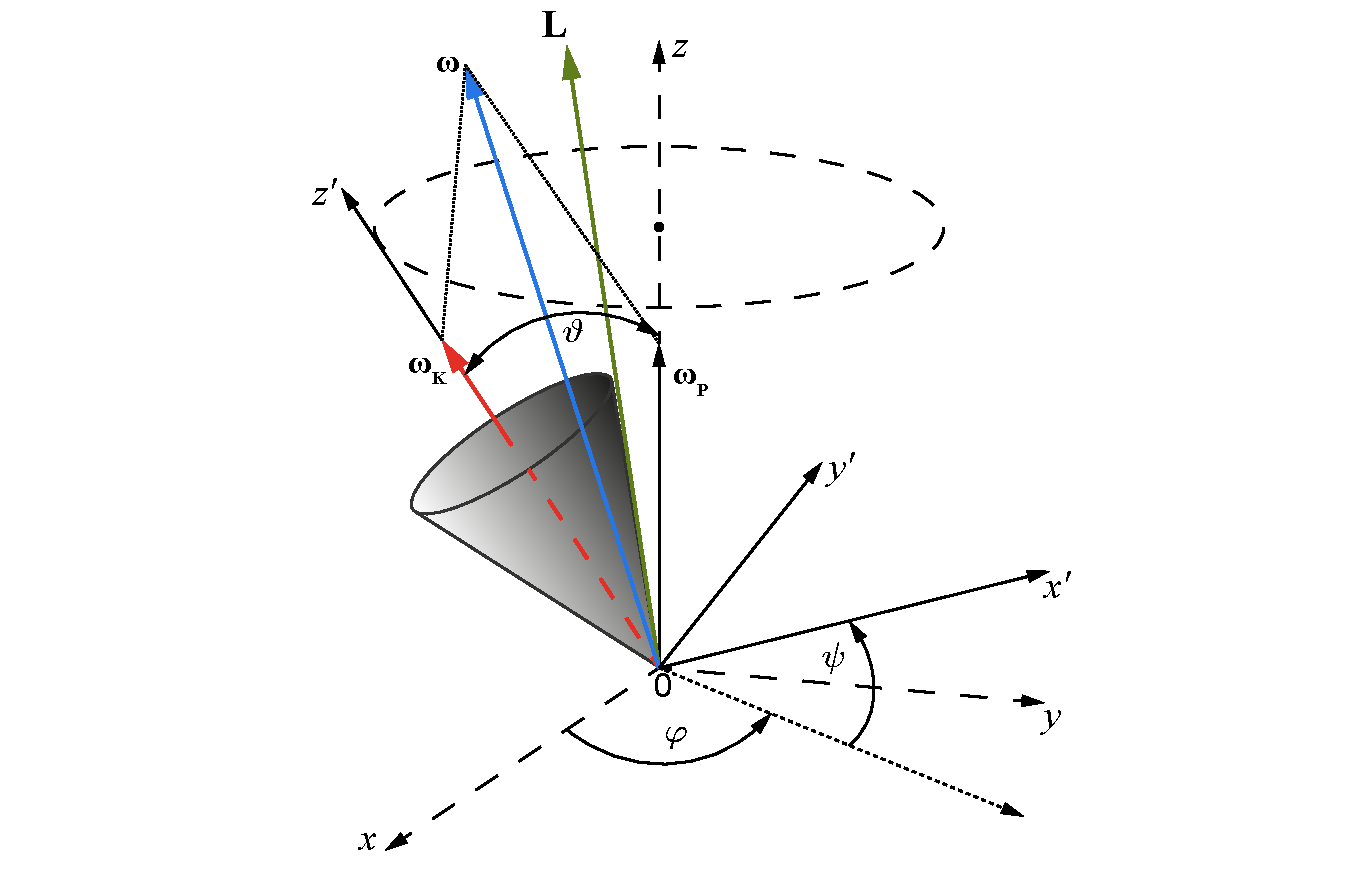
\includegraphics[width=\textwidth]{Unwucht03.pdf}
\caption[Gef�hrter Kreisel als Umkehrung eines Rotors mit Unwucht.]{Gef�hrter Kreisel als Umkehrung eines Rotors mit Unwucht.} 
\label{abb:bew_unwucht03}
\end{figure}
    \begin{align*}
        \dot{\vec{L}}_\text{ZM} = m_\text{ZM}\,\omega^2 \begin{vmatrix}
        \vec{e}_x & \vec{e}_y & \vec{e}_z\\
        \sin\vartheta & 0 & \cos\vartheta \\
        -\frac{D^2}{2}\,\sin\vartheta + x_\text{ZM}\,\cos\vartheta & 0 & -x_\text{ZM}\,D\,\sin\vartheta + 2x_\text{ZM}{}^2\,\cos\vartheta
        \end{vmatrix}
    \end{align*}
    Aus den Gleichungen \eqref{eq:bew_unwucht05} und \eqref{eq:bew_unwucht04} folgt dann:
    \begin{align}
        m_\text{ZM} = \frac{\lk J_1-J_3\rk\,\sin\lk 2\vartheta\rk}{2x_\text{ZM}\,D\,\cos\lk 2\vartheta\rk + \lk 2x_\text{ZM}{}^2-D^2 /2 \rk\,\sin\lk 2\vartheta\rk } \,.  \label{eq:bew_unwucht07}
    \end{align}
    Wir k�nnen f�r die Tr�gheitsmomente des Reifens schreiben ($m_\text{R}$ Masse des Reifens):
    \begin{align*}
        J_1 &= \frac{M_\text{R}}{4}\,\lk \frac{D^2}{3}+R^2\rk \,,~~~~ J_3 = \frac{m_\text{R}}{2}\,R^2\,,
    \end{align*}
    woraus folgt:
    \begin{align}
        m_\text{ZM} = \frac{m_\text{R}\,\lk \frac{D^2}{3}-R^2\rk\,\sin\vartheta\,\cos\vartheta}{8\lk x_\text{ZM}\,\sin\vartheta + \frac{D}{2}\,\cos\vartheta\rk\lk x_\text{ZM}\,\cos\vartheta - \frac{D}{2}\,\sin\vartheta\rk} \,. \label{eq:bew_unwucht08}
    \end{align}
    Wie zu erwarten war, h�ngt die Zusatzmasse vom Unwuchtwinkel $\vartheta$ und der Geometrie (D, R) des Reifens ab. Da $m_\text{ZM}>0$ sein muss (man k�nnte nat�rlich auch Massenelemente des Reifens entfernen, das wollen wir aber nicht betrachten), kann man folgende F�lle unterscheiden ($0\leq \vartheta\leq \frac{\pi}{2}$):
    \begin{enumerate}
        \item [1)]
        \begin{align*}
        R &< \frac{D}{\sqrt{3}} \rightarrow ~~~~ x_\text{ZM} > \frac{D}{2}\,\tan\vartheta  \,,  
        \end{align*}
        \item [2)]
        \begin{align*}
        R = \frac{D}{\sqrt{3}} ~~~~ \rightarrow ~~~~ \text{keine Auswuchtung notwendig}  \,,
        \end{align*}
        \item [3)]
        \begin{align*}
            R&>\frac{D}{\sqrt{3}} ~~~~ \text{(typ. Form eines Rades)}~~~~   \rightarrow ~~~~ x_\text{ZM} < \frac{D}{2}\,\tan\vartheta \,.
        \end{align*}
    \end{enumerate}
    Der betrachtete Fall ist etwas theoretisch, zeigt aber das Grundprinzip. Beim Auswuchten eines Autoreifens einer Autofelge werden meist zwei verschiedene Massen auf der Innen und Au�enseite der Felge befestigt, sie befinden sich im Allgemeinen nicht symmetrisch zueinander im Bezug auf die Rotationsachse. Dem Leser wird dies als erweiterte �bung empfohlen. 
\begin{figure}
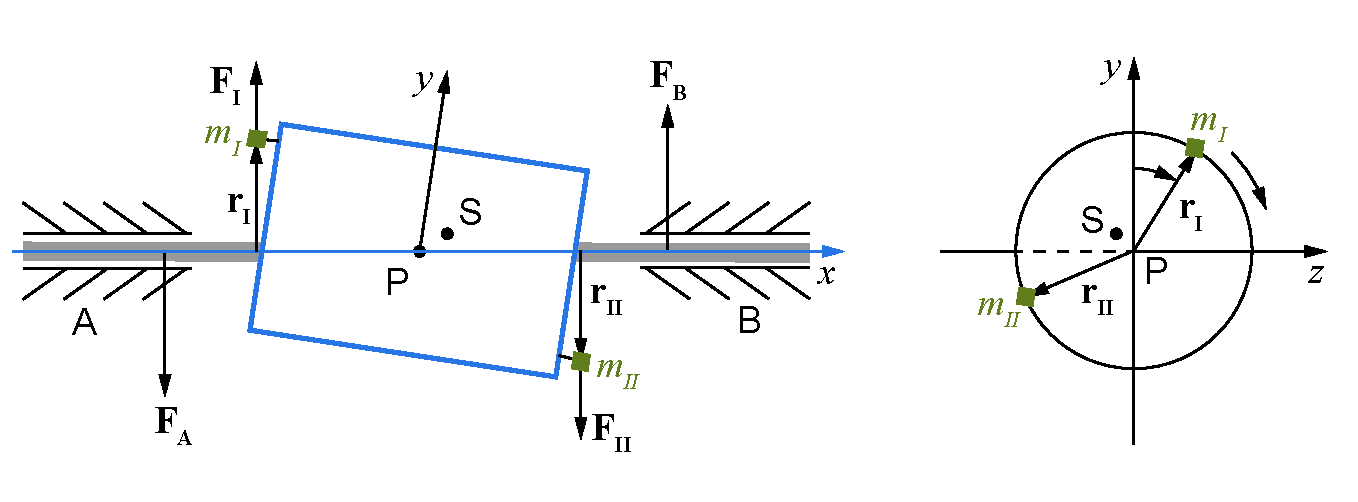
\includegraphics[width=\textwidth]{Unwucht04.pdf}
\caption[Allgemeiner Fall des Auswuchtens von Rotoren]{Allgemeiner Fall des Auswuchtens von Rotoren} 
\label{abb:bew_unwucht04}
\end{figure}

		Dazu m�ssen folgende Beziehungen erf�llt werden (\figref{bew_unwucht04}). Man beachte, dass wir in \figref{bew_unwucht04} das KOS $\vec{\Sigma'}$ gegen�ber \figref{bew_unwucht03} ver�ndert haben und dass auch der Schwerpunkt S nun nicht mehr auf der Drehachse liegt. $\vec{\Sigma'}$ ist aber auch hier ein k�rperfestes System, der Einfachheit halber lassen wir die Striche weg.
    \begin{align}
    \begin{split}
        \vec{F}_1 + \vec{F}_2 &= \vec{F}_\text{A}+\vec{F}_\text{B}\,,\\
        \vec{r}_{P1} \times \vec{F}_1 + \vec{r}_{P2} \times \vec{F}_2 &= \vec{r}_{P\text{A}} \times \vec{F}_\text{A} + \vec{r}_{P\text{B}} \times \vec{F}_\text{B}\,,
    \end{split}  \label{eq:bew_unwucht09}
    \end{align}
    \begin{align}
    \begin{split}
	     \vec{F}_1 &= m_1\,\omega^2\,\vec{r}_1 \,,~~\vec{F}_2 = m_2\,\omega^2\,\vec{r}_2\,, \\
      	\vec{F}_1 + \vec{F}_2 &= m\,\vec{\omega}\times \lk \vec{\omega}\times \vec{r}_{\text{P}S}\rk\,, ~~\vec{r}_{\text{P}1}\times \vec{F}_1 + \vec{r}_{\text{P}2} \times \vec{F}_2 = \vec{\omega} \times \vec{\Theta}_\text{P}\,\vec{\omega}\,.  \label{eq:bew_unwucht10}
    \end{split}  
    \end{align}
    mit:
    \begin{align}
    \begin{split}
        \vec{\omega} &= \begin{pmatrix}
        \omega \\ 0 \\ 0
        \end{pmatrix}\,, ~~~~
        \vec{r}_1 = \begin{pmatrix}
        0 \\ y_1\\z_1
        \end{pmatrix}\,, ~~~~
        \vec{r}_2 = \begin{pmatrix}
        0 \\ y_2\\z_2
        \end{pmatrix}\,, \\
        \vec{r}_{\text{P}1}&= \begin{pmatrix}
        x_{\text{P}1} \\ y_{\text{P}1} \\ z_{\text{P}1}
        \end{pmatrix} =  \begin{pmatrix}
        x_{\text{P}1} \\ y_{1} \\ z_{1}
        \end{pmatrix}   \,, ~~~~ 
        \vec{r}_{\text{P}2} = \begin{pmatrix}
        x_{\text{P}2} \\ y_{\text{P}2} \\ z_{\text{P}2}
        \end{pmatrix} =  \begin{pmatrix}
        x_{\text{P}2} \\ y_{2} \\ z_{2}
        \end{pmatrix} \,, \\
        \vec{\Theta}_\text{P} &= \begin{pmatrix}
        \Theta_{11\text{P}} & -\Theta_{12\text{P}} & -\Theta_{13\text{P}} \\
        -\Theta_{21\text{P}} & \Theta_{22\text{P}} & -\Theta_{23\text{P}} \\
        -\Theta_{31\text{P}} & -\Theta_{32\text{P}} & \Theta_{33\text{P}} 
        \end{pmatrix}\,.
    \end{split} \label{eq:bew_unwucht11}
    \end{align}
    Die L�sungen von \eqref{eq:bew_unwucht10} und \eqref{eq:bew_unwucht11} sind die beiden zum Auswuchten erforderlichen Vektoren $\vec{U}_1= m_1\,\vec{r}_1$ und $\vec{U}_2= m_2\,\vec{r}_2$ in den Ausgleichsebenen $1$ und $2$. 
\end{enumerate}

\end{sol} 
%\href{PhysikUncut_Part1.pdf#prb:bew_unwucht}{\textcolor{blue} {$\rightarrow$ zur \probref{bew_unwucht}.}}\\
\textcolor{blue} {$\rightarrow$ zur} \probref{bew_unwucht}.\\
\noindent\rule[1ex]{\textwidth}{0.5pt}  \newpage

%-----------------------------------------------------------------------------------------------------------
\hypertarget{lsg:bew_scheibe}{}
\begin{sol}{prob:bew_scheibe}\label{lsg:bew_scheibe} %�bung51
\textbf{Rollende Kreisscheibe und Reifen} \\ \\
Wir starten von der Lagrange-Funktion und ber�cksichtigen die Zwangsbedingungen \eqref{eq:bew_ZBrollendeScheibe1} und \eqref{eq:bew_ZBrollendeScheibe2} nach der Methode der Lagrange-Multiplikatoren. Wir wollen uns die Rechenarbeit etwas vereinfachen und benutzen f�r die Haupttr�gheitsmomente der Kreisscheibe 
	\[J_{12} = \frac{m}{4}\,R^2, ~~~~~J_3 = \frac{m}{2}\,R^2	\]
und f�r den Reifen 
	\[J_{12} = \frac{m}{2}\,R^2, ~~~~~J_3 = m\,R^2\,.\]
Die Lagrange-Funktion lautet dann f�r die \emph{Kreisscheibe} :
\begin{align}
\begin{split}
    \mathcal{L} = \:&\frac{m}{2}\,\Bigg( \dot{x}_\text{A}{}^2+\dot{y}_\text{A}{}^2 + R^2\,\lek \frac{\dot{\varphi}^2}{4}\,\lk 1+5\cos^2\vartheta\rk + \frac{5}{4}\,\dot{\vartheta}^2+ \frac{\dot{\psi}^2}{2} + \dot{\varphi}\,\dot{\psi}\,\cos\vartheta\rek\\
    &-2R\,\dot{x}_\text{A}\,\lek\dot{\varphi}\,\cos\varphi\,\cos\vartheta - \dot{\vartheta}\,\sin\varphi\,\sin\vartheta\rek \\
    &-2R\,\dot{y}_\text{A}\lek \dot{\varphi}\,\sin\varphi\,\cos\vartheta + \dot{\vartheta}\,\cos\varphi\,\sin\vartheta\rek\Bigg) - m\,g\,R\,\sin\vartheta\,. 
\end{split} \label{eq:bew_rolldisk01}
\end{align}
Entsprechend f�r den \emph{Reifen}:
\begin{align}
\begin{split}
    \mathcal{L} = \:&\frac{m}{2}\,\Bigg( \dot{x}_\text{A}{}^2+\dot{y}_\text{A}{}^2 + R^2\,\lek \frac{\dot{\varphi}^2}{2}\,\lk 1+3\cos^2\vartheta\rk + \frac{3}{2}\,\dot{\vartheta}^2+ \dot{\psi}^2+ 2\dot{\varphi}\,\dot{\psi}\,\cos\vartheta\rek\\
    &-2R\,\dot{x}_\text{A}\,\lek\dot{\varphi}\,\cos\varphi\,\cos\vartheta - \dot{\vartheta}\,\sin\varphi\,\sin\vartheta\rek \\
    &-2R\,\dot{y}_\text{A}\lek \dot{\varphi}\,\sin\varphi\,\cos\vartheta + \dot{\vartheta}\,\cos\varphi\,\sin\vartheta\rek\Bigg) - m\,g\,R\,\sin\vartheta\,. 
\end{split} \label{eq:bew_rolldisk02}
\end{align}
Wir sehen, dass sich die Lagrange-Funktionen f�r den Reifen und die Kreisscheibe gleicher Masse wie erwartet nur im Rotationsterm unterscheiden . \\
Wir berechnen nun f�r die Aufstellung der Lagrange-Gleichung 1. Art nach Kapitel \ref{kap:bew_Lagrange_I} die Zwangskr�fte nach \eqref{eq:bew_Zwangskraefte}:
\begin{align}
    Z_j = \sum_{r=1}^{Z_\text{B}}\,\lambda_r\,a_{rj} ~~~~ \text{mit} ~~~~ 0 = \sum_{j=1}^F\,a_{rj}\,\D q_{j} \,. \label{eq:bew_rolldisk03}
\end{align}
In unserem Fall ist $F= 5$ und $Z_\text{B} = 2$, also $r=1\ldots 2$ und die $q_j$ mit $j= 1\ldots 5$ sind gegeben durch:
\begin{align}
    q_1 = x_\text{A}\,, ~~~~ q_2 = y_\text{A}\,, ~~~~ q_3=\varphi\,, ~~~~ q_4 = \psi ~~~~ \text{und} ~~~~ q_5=\vartheta\,. \label{eq:bew_rolldisk04}
\end{align}
Die Zwangsbedingungen k�nnen wir differentiell aufschreiben:
\begin{align}
    f_1 = \D x_\text{A} + R\,\cos\varphi\,\D \psi ~~~~ f_2 = \D y_\text{A} + R\,\sin\varphi\,\D \psi \,. \label{eq:bew_rolldisk05}
\end{align}
Damit ergeben sich die $a_{rj}$ (aus dem Vergleich von \eqref{eq:bew_rolldisk05} mit \eqref{eq:bew_rolldisk03}) zu:
\begin{align*}
    a_{11} = 1\, ~~~~ a_{12} = 0\,, ~~~~  a_{13} = 0\,, ~~~~  a_{14} = R\,\cos\varphi\,, ~~~~  a_{15} = 0\,, \\
    a_{21} = 0\, ~~~~ a_{22} = 1\,, ~~~~  a_{23} = 0\,, ~~~~  a_{14} = R\,\sin\varphi\,, ~~~~  a_{25} = 0\,.
\end{align*}
Die Lagrange-Gleichungen 1. Art lauten dann f�r die Kreisscheibe:
\begin{subequations}
\begin{align}
    x_\text{A}&: ~~~~ m\,\frac{\D^2}{\D t^2}\,\lk x_\text{A} - R\,\sin\varphi\,\cos\vartheta\rk = \lambda_1 \label{eq:bew_rolldisk06a}\\
    y_\text{A}&: ~~~~ m\,\frac{\D^2}{\D t^2}\,\lk y_\text{A} + R\,\cos\varphi\,\cos\vartheta\rk = \lambda_2 \label{eq:bew_rolldisk06b}\\
    \varphi&: ~~~~ R\,\frac{\D}{\D t}\lek \dot{\varphi} \lk 1+5\cos^2\vartheta\rk +2\dot{\psi}\,\cos\vartheta\rek -4\cos\vartheta\,\lk \ddot{x}_\text{A}\,\cos\varphi + \ddot{y}_\text{A}\,\sin\varphi\rk = 0 \label{eq:bew_rolldisk06c}\\
    \psi&: ~~~~ \frac{m}{2}\,R\,\frac{\D}{\D t}\,\lk \dot{\psi} + \dot{\varphi}\,\cos\vartheta\rk = \lambda_1\,\cos\varphi + \lambda_2\,\sin\varphi\label{eq:bew_rolldisk06d} \\
    \vartheta&: ~~~~ \frac{5}{4}\,R\,\lk \ddot{\vartheta} + \dot{\varphi}^2\,\sin\vartheta\,\cos\vartheta\rk + \frac{R}{2}\,\dot{\varphi}\,\dot{\psi}\,\sin\vartheta + g\,\cos\vartheta  \nonumber \\
    &\, ~~~~~  + \sin\vartheta\lk \ddot{x}_\text{A}\,\sin\varphi - \ddot{y}_\text{A}\,\cos\varphi\rk = 0 \,. \label{eq:bew_rolldisk06e}
\end{align}\label{eq:bew_rolldisk06}
\end{subequations}
F�r den Reifen kann man das leicht �berleiten in:
\begin{subequations}
\begin{align}
    x_\text{A}&: ~~~~ m\,\frac{\D^2}{\D t^2}\,\lk x_\text{A} - R\,\sin\varphi\,\cos\vartheta\rk = \lambda_1  \label{eq:bew_rolldisk07a} \\
    y_\text{A}&: ~~~~ m\,\frac{\D^2}{\D t^2}\,\lk y_\text{A} + R\,\cos\varphi\,\cos\vartheta\rk = \lambda_2  \label{eq:bew_rolldisk07b} \\
    \varphi&: ~~~~ R\,\frac{\D}{\D t}\lek \dot{\varphi}\lk 1+3\cos^2\vartheta\rk  + 2\dot{\psi}\,\cos\vartheta\rek -2\cos\vartheta\lk \ddot{x}_\text{A}\,\cos\varphi + \ddot{y}_\text{A}\,\sin\varphi\rk = 0 \label{eq:bew_rolldisk07c}\\
    \psi&: ~~~~ m\,R\,\frac{\D}{\D t}\,\lek \dot{\psi}+\dot{\varphi}\,\cos\vartheta\rek = \lambda_1\,\cos\varphi + \lambda_2\,\sin\varphi\\
    \vartheta&: ~~~~ \frac{3}{2}R\,\lk \ddot{\vartheta} + \dot{\varphi}^2\,\sin\vartheta\,\cos\vartheta\rk + R\,\dot{\varphi}\,\dot{\psi}\,\sin\vartheta + g\,\cos\vartheta  \nonumber \\
    &\, ~~~~~ + \sin\vartheta\lk \ddot{x}_\text{A}\,\sin\varphi - \ddot{y}_\text{A}\,\cos\varphi\rk = 0\,. \label{eq:bew_rolldisk07e}
\end{align} \label{eq:bew_rolldisk07}
\end{subequations}

Damit haben wir f�nf Gleichungen f�r 7 Unbekannte $x_\text{A}, y_\text{A}, \varphi, \psi, \vartheta$ und $\lambda_1, \lambda_2$.\\
Wir brauchen also noch die beiden Zwangsbedingungen, die f�r die Scheibe und Reifen gleich lauten. Wir leiten diese zweimal nach der Zeit ab:
\begin{align}
\begin{split}
    \dot{f}_1 \rightarrow \ddot{x}_\text{A} &= -R\,\frac{\D}{\D t}\lk \cos\varphi\,\dot{\psi}\rk \\
    \dot{f}_2 \rightarrow \ddot{y}_\text{A} &= -R\,\frac{\D}{\D t}\lk \sin\varphi\,\dot{\psi}\rk
\end{split}  \label{eq:bew_rolldisk08}
\end{align}
Damit haben wir nun 7 Bestimmungsgleichungen und k�nnen als erstes $\lambda_1$ und $\lambda_2$ eliminieren. Wir benutzen dazu \eqref{eq:bew_rolldisk06a}, \eqref{eq:bew_rolldisk06b} \bzw \eqref{eq:bew_rolldisk07a}, \eqref{eq:bew_rolldisk07b}, setzen diese in die Gleichungen \eqref{eq:bew_rolldisk08} ein und erhalten:
\begin{align}
\begin{split}
    \lambda_1 &= -m\,R\,\frac{\D}{\D t}\,\lek \dot{\psi}\,\cos\varphi + \frac{\D}{\D t}\,\lk \sin\varphi\,\cos\vartheta\rk\rek \,,\\
     \lambda_2 &= -m\,R\,\frac{\D}{\D t}\,\lek \dot{\psi}\,\sin\varphi - \frac{\D}{\D t}\,\lk \cos\varphi\,\cos\vartheta\rk\rek \,.
\end{split} \label{eq:bew_rolldisk09}
\end{align}
Damit haben wir die Zwangsbedingungen �ber die Lagrange-Multiplikatoren verarbeitet und k�nnen nun die Bewegungsgleichungen f�r die Euler-Winkel\footnote{Wir machen damit aus den quasi-generalisierten Koordinaten in \eqref{eq:bew_rolldisk06} bzw. \eqref{eq:bew_rolldisk07} echte generalisierte Koordinaten.} aufstellen. Dazu setzen wir \eqref{eq:bew_rolldisk09} in \eqref{eq:bew_rolldisk06d} ein und erhalten zun�chst:
\begin{align*}
    \frac{m}{2}\,R\,\frac{\D}{\D t}\,\lk\dot{\psi} + \dot{\varphi}\,\cos\vartheta\rk = &- m\,R\,\frac{\D}{\D t} \underbrace{\lek\dot{\psi} \,\cos\varphi + \frac{\D}{\D t} \lk \sin\varphi\,\cos\vartheta\rk\rek}_{\substack{T_1}}\,\cos\varphi \\
    &- m\,R\,\frac{\D}{\D t} \underbrace{\lek\dot{\psi} \,\sin\varphi - \frac{\D}{\D t} \lk \cos\varphi\,\cos\vartheta\rk\rek}_{\substack{T_2}}\,\sin\varphi
\end{align*}

�ber die Zwischenschritte:
\begin{align*}
    \ddot{\psi} + \ddot{\varphi}\,\cos\vartheta - \dot{\varphi}\,\dot{\vartheta}\,\sin\vartheta &= -2\ddot{\psi} - 2\ddot{\varphi}\,\cos\vartheta + 4\,\dot{\varphi}\,\dot{\vartheta}\,\sin\vartheta \\
    3\lk \ddot{\psi} + \ddot{\varphi} \,\cos\vartheta \rk - 5\dot{\varphi}\,\dot{\vartheta}\,\sin\vartheta &= 0\,,
\end{align*}
erhalten wir dann eine (zun�chst noch mit $\ddot{\varphi}$ verkoppelte) Bewegungsgleichung f�r $\psi$ 
\begin{subequations}
\begin{align} 
    \psi: ~~~~ \ddot{\psi} + \ddot{\varphi}\,\cos\vartheta - \frac{5}{3}\,\dot{\varphi}\,\dot{\vartheta}\,\sin\vartheta &= 0 \,~~\text{Kreisscheibe}, \label{eq:bew_rolldisk10a}\\
    \psi: ~~~~ \ddot{\psi} + \ddot{\varphi}\,\cos\vartheta - \frac{3}{2}\,\dot{\varphi}\,\dot{\vartheta}\,\sin\vartheta &= 0 \,~~\text{Reifen}. \label{eq:bew_rolldisk10b}
\end{align}
\end{subequations}
Aus den Zwangsbedingungen k�nnen wir �ber 
\begin{subequations}
\begin{align}
    &\dot{x}_\text{A} + R\,\dot{\psi}\,\cos\varphi = 0 \nonumber \\
    &\ddot{x}_\text{A} + R\,\ddot{\psi}\,\cos\varphi - R\,\dot{\varphi}\,\dot{\psi}\,\sin\varphi = 0 ~~~~ \Big | \cdot \cos\varphi \nonumber \\
    &\ddot{x}_\text{A}\,\cos\varphi + R\,\ddot{\psi}\,\cos^2\varphi - R\,\dot{\varphi}\,\dot{\psi}\,\sin\varphi\,\cos\varphi = 0 \label{eq:bew_rolldisk11a} \\
    &\dot{y}_\text{A} + R\,\dot{\psi}\,\sin\varphi = 0 \nonumber \\
    &\ddot{y}_\text{A} + R\,\ddot{\psi}\,\sin\varphi + R\,\dot{\varphi}\,\dot{\psi}\,\cos\varphi = 0 ~~~~ \Big | \cdot \sin\varphi \nonumber  \\
    &\ddot{y}_\text{A}\,\sin\varphi + R\,\ddot{\psi}\,\sin^2\varphi + R\,\dot{\varphi}\,\dot{\psi}\,\sin\varphi\,\cos\varphi = 0 \label{eq:bew_rolldisk11b} 
\end{align}
\end{subequations}
die folgenden Beziehungen ableiten:
\begin{align}
    \ddot{x}_\text{A}\,\cos\varphi + \ddot{y}_\text{A}\,\sin\varphi = -R\,\ddot{\psi}\,, ~~~
		\ddot{x}_\text{A}\,\sin\varphi - \ddot{y}_\text{A}\,\cos\varphi = +R\,\dot{\varphi}\,\dot{\psi} \,.
\label{eq:bew_rolldisk12} 
\end{align}
Diese setzen wir in die verbleibenden Gleichungen \eqref{eq:bew_rolldisk06c} und \eqref{eq:bew_rolldisk06e} bzw. \eqref{eq:bew_rolldisk07c} und \eqref{eq:bew_rolldisk07e} ein und erhalten wir schlie�lich f�r alle drei Euler-Winkel $\varphi, \psi$ und $\vartheta$ die folgenden Bewegungsgleichungen f�r die Kreisscheibe:
\begin{subequations}
\begin{align}
    &\psi: ~~~~ \ddot{\psi} + \ddot{\varphi}\,\cos\vartheta - \frac{5}{3}\,\dot{\varphi}\,\dot{\vartheta}\,\sin\vartheta = 0  \label{eq:bew_rolldisk13a}\\
    &\varphi: ~~~~ \frac{\D}{\D t}\,\lek \dot{\varphi}\,\lk 1+5\cos^2\,\vartheta\rk + 2\dot{\psi}\,\cos\vartheta\rek + 4\ddot{\psi}\,\cos\vartheta = 0 \label{eq:bew_rolldisk13b} \\
    & ~~~~\rightarrow ~~~ \ddot{\varphi}\,\lk 1+5\cos^2\,\vartheta\rk -10\dot{\varphi}\dot{\vartheta}\cos\vartheta\,\sin\vartheta + 6\ddot{\psi}\,\cos\vartheta - 2\dot{\psi}\dot{\vartheta}\,\sin\vartheta = 0 \notag \\ 
    &\vartheta: ~~~~  \ddot{\vartheta} + \dot{\varphi}^2\,\sin^2\vartheta\,\cos\vartheta + \frac{6}{5}\,\dot{\varphi}\,\dot{\psi}\,\sin\vartheta + \frac{4}{5}\frac{g}{R}\,\cos\vartheta = 0 \,, \label{eq:bew_rolldisk13c}
\end{align}
\end{subequations}
\bzw f�r den Reifen: 
\begin{subequations}
\begin{align}
    &\psi: ~~~~ \ddot{\psi} + \ddot{\varphi}\,\cos\vartheta - \frac{3}{2}\,\dot{\varphi}\,\dot{\vartheta}\,\sin\vartheta = 0 \label{eq:bew_rolldisk14a} \\
		&\varphi: ~~~~ \frac{\D}{\D t}\,\lek \dot{\varphi}\,\lk 1+3\cos^2\,\vartheta\rk + 2\dot{\psi}\,\cos\vartheta\rek + 2\ddot{\psi}\,\cos\vartheta = 0 \label{eq:bew_rolldisk14b}\\  
    & ~~~~\rightarrow ~~~ \ddot{\varphi}\,\lk 1+3\cos^2\,\vartheta\rk -6\dot{\varphi}\dot{\vartheta}\cos\vartheta\,\sin\vartheta + 4\ddot{\psi}\,\cos\vartheta - 2\dot{\psi}\dot{\vartheta}\,\sin\vartheta = 0  \notag \\
    &\vartheta: ~~~~ \ddot{\vartheta} + \dot{\varphi}^2\,\sin^2\vartheta\,\cos\vartheta  + \frac{4}{3} \dot{\varphi}\,\dot{\psi}\,\sin\vartheta + \frac{2}{3}\frac{g}{R}\,\cos\vartheta = 0 \,.\label{eq:bew_rolldisk14c}
\end{align}
\end{subequations}

Wir m�ssen nun noch die Gleichungen f�r $\varphi$ und $\psi$ hinsichtlich der 2. Ableitung der jeweiligen anderen Koordinate entkoppeln.
Wir multiplizieren dazu \eqref{eq:bew_rolldisk13a} mit $6\cos\vartheta$, subtrahieren die erhaltene Gleichung von \eqref{eq:bew_rolldisk13b} und erhalten 
	\[     \ddot{\varphi}\, \sin\vartheta - 2 \dot{\psi}\dot{\vartheta} = 0 \,,
\]
was bereits die entkoppelte Gleichung f�r $\ddot{\varphi}$ ergibt. Diese Gleichung multiplizieren wir mit $\cos\vartheta$ und subtrahieren dies von der mit $\sin\vartheta$ multiplizierten Gleichung \eqref{eq:bew_rolldisk13a}, wodurch wir die endg�ltige Form der Gleichung f�r die Euler-Winkel erhalten \eqref{eq:bew_rollendescheibe_dgls}, und zwar f�r die Kreisscheibe:
\begin{subequations}
  \begin{align}
    &\varphi: ~~~~ \ddot{\varphi}\,\sin\vartheta - 2 \dot{\psi}\dot{\vartheta} = 0 \; , \\
    &\psi: ~~~~ \ddot{\psi}\, \sin\vartheta - \frac{5}{3}\, \dot{\varphi}\,
    \dot{\vartheta} \sin^2\vartheta  + 2  \dot{\psi}\,\dot{\vartheta} \cos\vartheta  = 0 \;, \\
    &\vartheta: ~~~~ \ddot{\vartheta} + \dot{\varphi}^2 \sin\vartheta\, \cos\vartheta\,
    + \frac{6}{5} \dot{\varphi}\,\dot{\psi} \, \sin\vartheta\
    + \frac{4}{5} \frac{g}{R} \cos\vartheta = 0 \; ,
                                                                       \label{eq:eq:bew_rollendescheibe_S}
  \end{align}
  \label{eq:bew_rollendescheibe_dgl_S}
\end{subequations}
\bzw den Reifen:
\begin{subequations}
  \begin{align}
	  &\varphi: ~~~~ \ddot{\varphi}\,\sin\vartheta  - 2 \dot{\psi}\dot{\vartheta} = 0 \; , \\
    &\psi: ~~~~ \ddot{\psi}\, \sin\vartheta - \frac{3}{2}\,\dot{\varphi}\,
    \dot{\vartheta} \sin^2\vartheta  + 2 \dot{\psi}\,\dot{\vartheta}\cos\vartheta\,  = 0 \;,\\
    &\vartheta: ~~~~ \ddot{\vartheta} + \dot{\varphi}^2 \,\sin\vartheta\, \cos\vartheta\,
    + \frac{4}{3} \dot{\varphi}\,\dot{\psi} \, \sin\vartheta
    + \frac{2}{3} \frac{g}{R} \cos\vartheta = 0 \; .
                                                                       \label{eq:eq:bew_rollendescheibe_R}
  \end{align}
  \label{eq:bew_rollendescheibe_dgl_R}
\end{subequations}

In \figref{bew_ScheibeReifen01} ist die zeitliche Entwicklung der Euler-Winkel als auch der Trajektorie des Auflagepunktes jeweils f�r Kreisscheibe und Reifen dargestellt.
Deutlich zu erkennen ist, dass der Reifen wegen des gr��eren Drehimpulses (bei gleicher Masse) eine \anf{stabilere} Bahn hat.
Im \mscr~\mlbewref{RollendesRad.m} ist die numerische Berechnung als auch eine Simulation der Bewegung hinterlegt.

\begin{figure}
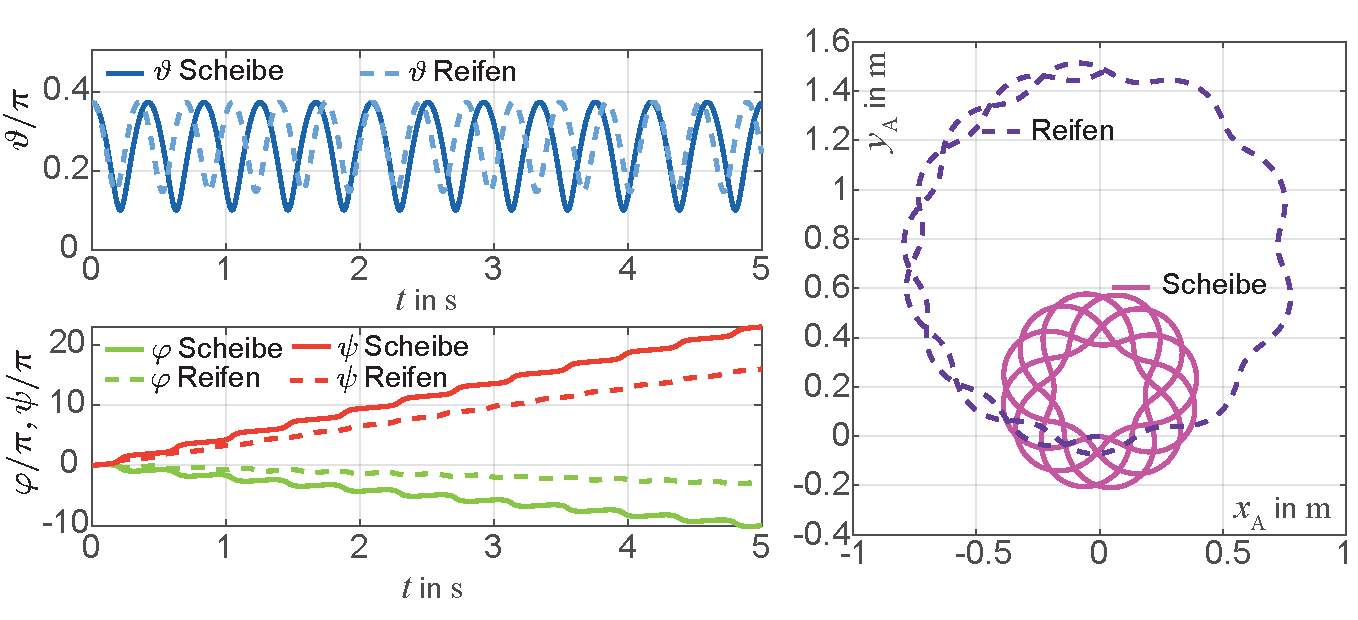
\includegraphics[width=\textwidth]{ScheibeReifen01.pdf}
  \caption[Rollen einer Scheibe und eines Reifens auf ebener Fl�che im Vergleich.]{Rollen einer Scheibe und eines Reifens auf ebener Fl�che im Vergleich. Parameter: $R = \SI{0.15}{\metre}, \varphi_0 = 0, \vartheta_0 = 3\pi/8, \psi_0 = 0, \omega_{\varphi}   = \SI{5.0}{\radian\per\second}, \omega_\vartheta = \SI{0.0}{\radian\per\second}, \omega_\psi= \SI{6.0}{\radian\per\second}$. Deutlich zu erkennen ist, dass der Reifen wegen des gr��eren Drehimpulses (bei gleicher Masse) eine "`stabilere"' Bahn hat.} \label{abb:bew_ScheibeReifen01}
\end{figure}

\newpage
\begin{nebenrechnung}

\begin{align*}
    \frac{1}{2} \lk \ddot{\psi}+\ddot{\varphi}\,\cos\vartheta - \dot{\varphi}\,\sin\vartheta\,\dot{\vartheta} \rk = -\lk \frac{\D}{\D t} \lek T_1\rek\,\cos\varphi + \frac{\D}{\D t}\,\lek T_2\rek \,\sin\varphi\rk
\end{align*}
\begin{align*}
    \frac{\D}{\D t}\,\lek T_1\rek =\, &\frac{\D}{\D t}\,\lek \dot{\psi}\,\cos\varphi + \dot{\varphi}\,\cos\varphi\,\cos\vartheta - \dot{\vartheta} \,\sin\varphi\,\sin\vartheta\rek \\
    =\, &\ddot{\psi}\,\cos\varphi-\dot{\psi}\,\dot{\varphi}\,\sin\varphi + \ddot{\varphi}\,\cos\varphi\,\cos\vartheta - \dot{\varphi}^2\,\sin\varphi\,\cos\vartheta - \dot{\varphi}\,\dot{\vartheta}\,\cos\varphi\,\sin\vartheta \\
    &- \ddot{\vartheta}\,\sin\varphi\,\sin\vartheta - \dot{\vartheta}\,\dot{\varphi}\,\cos\varphi\,\sin\vartheta - \dot{\vartheta}^2\,\sin\varphi\,\cos\vartheta
\end{align*}
\begin{align*}
    \frac{\D}{\D t}\,\lek T_1\rek\,\cos\varphi = \, &\ddot{\psi}\,\cos^2\varphi - \killA{\dot{\psi}\,\dot{\varphi}\,\sin\varphi\,\cos\varphi} + \ddot{\varphi}\,\cos^2\varphi\,\cos\vartheta - \killA{\dot{\varphi}^2\,\sin\varphi\,\cos\varphi\,\cos\vartheta} \\
    &-\dot{\varphi}\,\dot{\vartheta}\,\cos^2\varphi\,\sin\vartheta- \killB{\ddot{\vartheta}\,\sin\varphi\,\cos\varphi\,\sin\vartheta} - \dot{\vartheta}\,\dot{\varphi}\,\cos^2\varphi\,\sin\vartheta - \killB{\dot{\vartheta}^2\,\sin\varphi\,\cos\varphi\,\cos\vartheta}
\end{align*}
\begin{align*}
    \frac{\D}{\D t}\,\lek T_2\rek =\, &\frac{\D}{\D t}\,\lek \dot{\psi}\,\sin\varphi + \dot{\varphi}\,\sin\varphi\,\cos\vartheta + \dot{\vartheta} \,\cos\varphi\,\sin\vartheta\rek \\
    =\, &\ddot{\psi}\,\sin\varphi + \dot{\psi}\,\dot{\varphi}\,\cos\varphi + \ddot{\varphi}\,\sin\varphi\,\cos\vartheta + \dot{\varphi}^2\,\cos\varphi\,\cos\vartheta - \dot{\varphi}\,\dot{\vartheta}\,\sin\varphi\,\sin\vartheta \\
    &+ \ddot{\vartheta}\,\cos\varphi\,\sin\vartheta - \dot{\vartheta}\,\dot{\varphi}\,\sin\varphi\,\sin\vartheta + \dot{\vartheta}^2\,\cos\varphi\,\cos\vartheta
\end{align*}
\begin{align*}
    \frac{\D}{\D t}\,\lek T_2\rek\,\sin\varphi = \, &\ddot{\psi}\,\sin^2\varphi + \killA{\dot{\psi}\,\dot{\varphi}\,\sin\varphi\,\cos\varphi} + \ddot{\varphi}\,\sin^2\varphi\,\cos\vartheta + \killA{\dot{\varphi}^2\,\sin\varphi\,\cos\varphi\,\cos\vartheta} \\
    &-\dot{\varphi}\,\dot{\vartheta} \,\sin^2\varphi\,\sin\vartheta + \killB{\ddot{\vartheta}\,\sin\varphi\,\cos\varphi\,\sin\vartheta} - \dot{\vartheta}\,\dot{\varphi}\,\sin^2\varphi\,\sin\vartheta + \killB{\dot{\vartheta}^2\,\sin\varphi\,\cos\varphi\,\cos\vartheta}
\end{align*}
\begin{align*}
    \frac{\D}{\D t}\,\lek T_1\rek\,\cos\varphi + \frac{\D}{\D t}\,\lek T_2\rek\,\sin\varphi &= \ddot{\psi} + \ddot{\varphi}\,\cos\vartheta - \dot{\varphi}\,\dot{\vartheta}\,\sin\vartheta - \dot{\varphi}\,\dot{\vartheta}\,\sin\vartheta \\
    &= \ddot{\psi} + \ddot{\varphi}\,\cos\vartheta - 2\dot{\varphi}\,\dot{\vartheta} \,\sin\vartheta
\end{align*}

\end{nebenrechnung}

\end{sol} 
%\href{PhysikUncut_Part1.pdf#prb:bew_scheibe}{\textcolor{blue} {$\rightarrow$ zur \probref{bew_scheibe}.}}\\
\textcolor{blue} {$\rightarrow$ zur} \probref{bew_scheibe}.\\
\noindent\rule[1ex]{\textwidth}{0.5pt}  \newpage

%%-----------------------------------------------------------------------------------------------------------
\hypertarget{lsg:bew_scheibeR}{}
\begin{sol}{prob:bew_scheibeR}\label{lsg:bew_scheibeR} %�bung52
\textbf{Rollende Kreisscheibe mit Reibung} \\ \\
Wir k�nnen unmittelbar an das Ergebnis von �bung \probref{bew_scheibe} anschlie�en.
Um die Reibung zu ber�cksichtigen, m�sste man f�r jeden Freiheitsgrad, \dh f�r alle Euler-Winkel und den Koordinaten $x_\text{A}, y_\text{A}$ f�r des Auflagepunktes einen Reibungsterm vorsehen. Wir wollen zun�chst annehmen, dass die Reibung auf der Grundfl�che dominiert, betrachten die Reibung f�r die Koordinaten $\varphi, \psi$ gegeben durch einen linearen Term mit $-\eta_1\,\dot{\varphi}$ \bzw $-\eta_1\,\dot{\psi}$, w�hrend das "`Umfallen"' eher durch den Luftwiderstand und damit durch einen quadratischen Term mit 
$-\eta_2\,\dot{\vartheta}^2$ beschrieben werden kann.
Wir erhalten \zb f�r die Kreisscheibe
\begin{subequations}
  \begin{align}
    &\varphi: ~~~~ \ddot{\varphi}\,\sin\vartheta - 2 \dot{\psi}\dot{\vartheta} + \eta_1\,\dot{\varphi}= 0 \; , \\
    &\psi: ~~~~ \ddot{\psi}\, \sin\vartheta - \frac{5}{3}\, \dot{\varphi}\,
    \dot{\vartheta} \sin^2\vartheta  + 2  \dot{\psi}\,\dot{\vartheta} \cos\vartheta + \eta_1\dot{\psi} = 0 \;, \\
    &\vartheta: ~~~~ \ddot{\vartheta} + \dot{\varphi}^2 \sin\vartheta\, \cos\vartheta\,
    + \frac{6}{5} \dot{\varphi}\,\dot{\psi} \, \sin\vartheta\
    + \frac{4}{5} \frac{g}{R} \cos\vartheta + \eta_2\dot{\vartheta}^2= 0 \; ,
                                                                       \label{eq:eq:bew_rollendescheibe_Sr}
  \end{align}
  \label{eq:bew_rollendescheibe_dgl_Sr}
\end{subequations}
%\begin{subequations}
  %\begin{align}
	  %&\varphi: ~~~~ \ddot{\varphi}\,\sin\vartheta  - 2 \dot{\psi}\dot{\vartheta} + \eta_1\,\dot{\varphi}= 0 \; , \\
    %&\psi: ~~~~ \ddot{\psi}\, \sin\vartheta - \frac{3}{2}\,\dot{\varphi}\,
    %\dot{\vartheta} \sin^2\vartheta  + 2 \dot{\psi}\,\dot{\vartheta}\cos\vartheta\, + \eta_1\dot{\psi} = 0 \;,\\
    %&\vartheta: ~~~~ \ddot{\vartheta} + \dot{\varphi}^2 \,\sin\vartheta\, \cos\vartheta\,
    %+ \frac{4}{3} \dot{\varphi}\,\dot{\psi} \, \sin\vartheta
    %+ \frac{2}{3} \frac{g}{R} \cos\vartheta + \eta_2\dot{\vartheta}^2= 0\; .
                                                                       %\label{eq:eq:bew_rollendescheibe_Rr}
  %\end{align}
  %\label{eq:bew_rollendescheibe_dgl_Rr}
%\end{subequations}

\begin{figure}
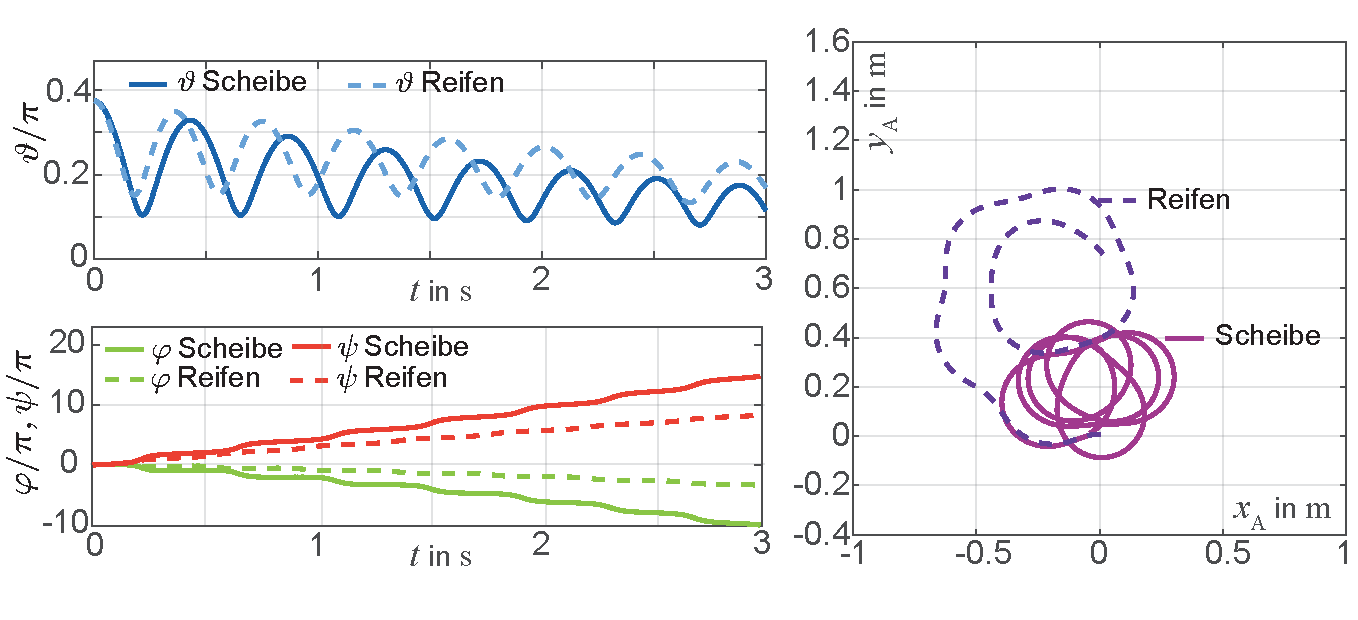
\includegraphics[width=\textwidth]{ScheibeReifen02.pdf}
  \caption[Rollen einer Scheibe und eines Reifens auf ebener Fl�che im Vergleich.]{Rollen einer Scheibe und eines Reifens auf ebener Fl�che im Vergleich. Parameter: $R = \SI{0.15}{\metre}, \varphi_0 = 0, \vartheta_0 = 3\pi/8, \psi_0 = 0, \omega_{\varphi}   = \SI{5.0}{\radian\per\second}, \omega_\vartheta = \SI{0.0}{\radian\per\second}, \omega_\psi= \SI{6.0}{\radian\per\second}$, Reibungsparameter f�r $\psi, \varphi: ~ \eta_1 = \SI{0.25}{\per\second}$, f�r $\vartheta : ~ \eta_2 = \SI{0.2}{\per\second\squared}\,$.} \label{abb:bew_ScheibeReifen02}
\end{figure}

In \figref{bew_ScheibeReifen02} ist die zeitliche Entwicklung der Euler-Winkel als auch der Trajektorie des Auflagepunktes jeweils f�r Kreisscheibe und Reifen dargestellt.
Im Vergleich zu \figref{bew_ScheibeReifen01} ist der Effekt der Reibung deutlich zu erkennen.
Der Reifen mit seinem gr��eren Drehimpulses (bei gleicher Masse) f�hrt weiterhin eine etwas \anf{stabilere} und gr��ere Bahnbewegung aus, wenn auch der Unterschied zur Scheibe gegen�ber dem reibungsfreien Fall geringer ist.
Im \mscr~\mlbewref{RollendesRadR.m} ist sowohl die numerische Berechnung, als auch eine Simulation der Bewegung hinterlegt.
Die Reibungsparameter sind gegen�ber realen Situationen �berh�ht, um die Effekte deutlich zu machen.

\end{sol} 
%\href{PhysikUncut_Part1.pdf#prb:bew_scheibeR}{\textcolor{blue} {$\rightarrow$ zur \probref{bew_scheibeR}.}}\\
\textcolor{blue} {$\rightarrow$ zur} \probref{bew_scheibeR}.\\
\noindent\rule[1ex]{\textwidth}{0.5pt}  \newpage

%-----------------------------------------------------------------------------------------------------------

\newpage
\hypertarget{lsg:bew_doubleconecomp}{}
\begin{sol}{prob:bew_doubleconecomp} \label{lsg:bew_doubleconecomp} %�bung53
\textbf{Der Doppelkegel -- Vergleich der inkorrekten bzw. N�herungs-Methoden mit der Berechnung in Kap. \ref{kap:bew_doublecone}} \\ \\
Wir wollen jetzt den Doppelkegel direkt im kartesischen KOS $\vec{\Sigma}$ berechnen. 
\begin{figure}
  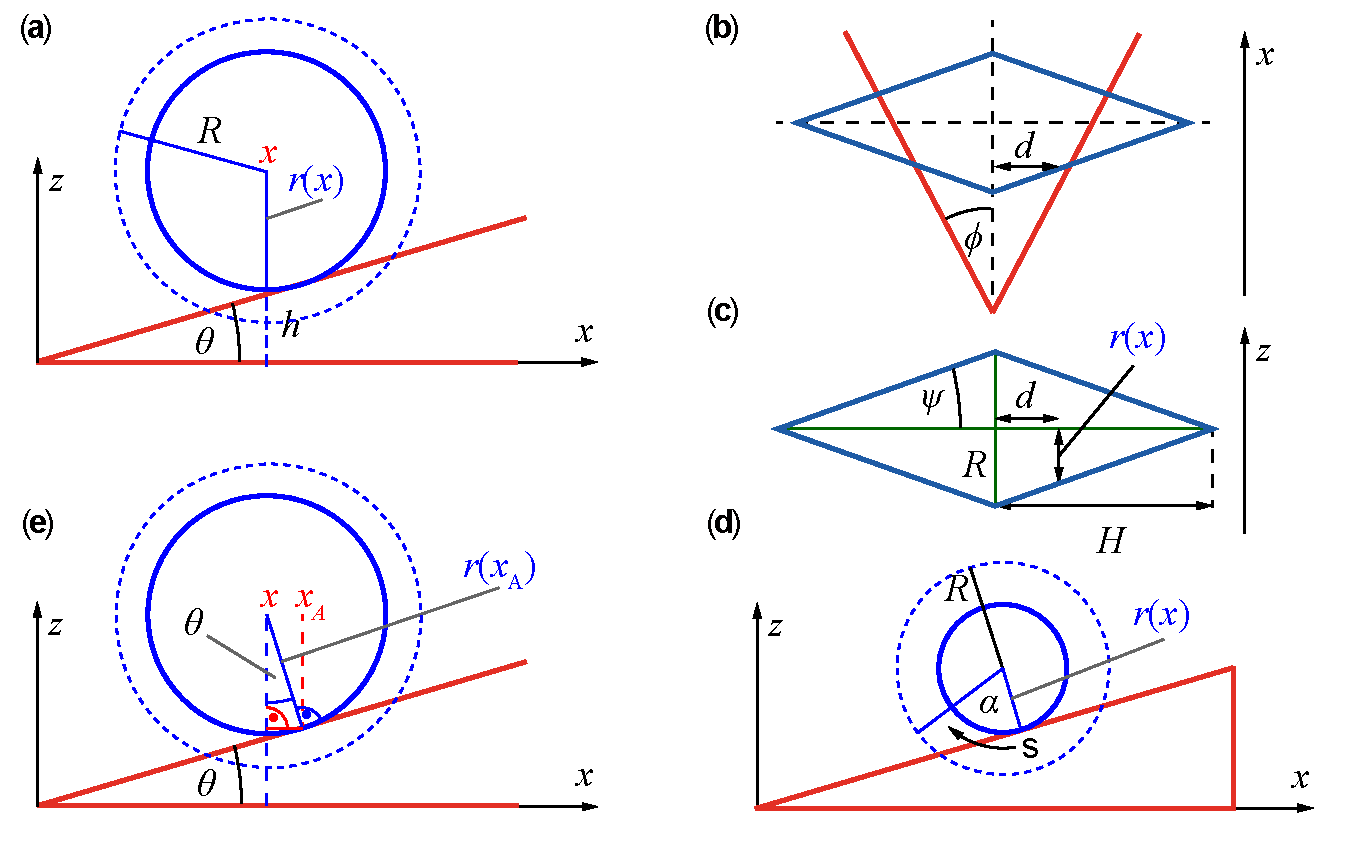
\includegraphics[width=\textwidth]{Doppelkegel0809.pdf}
  \caption[Geometrien zur Herleitung der Lagrange-Gleichung f�r den Doppelkegel.]{Geometrien zur Herleitung der Lagrange-Gleichung f�r den Doppelkegel im KOS $\vec{\Sigma}a$. \fa Rollpunkt unter Schwerpunkt \fb Draufsicht \fc Ansicht von hinten \fd Rollbedingung \fe Rollpunkt unter einem festen Winkel $\theta$ (Anstiegswinkel der Schienen).} \label{abb:bew_doublecone09}
\end{figure}
\begin{enumerate}
    \item [(A)] \emph{Rollpunkt unter Symmetrieachse}\\ \\
Im ersten Schritt wollen wir die N�herung machen, dass die Auflagepunkte des Doppelkegels direkt unter der Symmetrieachse liegen, was bei kleinen Winkeln $\phi$ und $\psi$ ann�hernd erf�llt ist. Aus \figref{bew_doublecone09}c-e kann man dann f�r die Koordinaten $x_\text{S}$ und $z_\text{S}$ des Schwerpunktes folgende Beziehungen ablesen, wobei wir den Subscript der Einfachheit halber weglassen. 
    \begin{align}
    \begin{split}
        d &\approx y\,\tan\phi\,, ~~\text{N�herung !} \\
        r\lk y\rk &\approx R-y\,\underbrace{\tan\phi\,\tan\psi}_{C_1} = R - y\, C_1\, \,~~\text{N�herung !} \,, \\
        \rightarrow ~~z\lk y\rk &= R + y\,\underbrace{\lk \tan\theta - \tan\phi\,\tan\psi\rk}_{C_2} = R + y\,C_2\,, \\
        \rightarrow ~~\dot{z}\lk y\rk &= C_2\,\dot{y}\,. \label{eq:bew_lsgdcone01}
    \end{split}
    \end{align}
    Jetzt m�ssen wir uns noch die Rotationsfrequenz des Kegels als Funktion des Ortes $y$ und der Geschwindigkeit $\dot{y}$ der Schwerpunktes beschaffen. Dazu betrachten wir \figref{bew_doublecone09}e und lesen ab:
    \begin{align}
    \begin{split}
        s\lk y\rk &= \frac{y}{\cos\theta} = r\lk y\rk\,\alpha\lk y\rk \,, \\
        \alpha\lk y\rk &= \frac{y}{\underbrace{\cos\theta}_{C_3}}\,\frac{1}{R-y\,\underbrace{\tan\phi\,\tan\psi}_{C_1}} = \frac{y}{C_3\,\lk R-y\,C_1\rk} \,,\\
        \rightarrow ~~\omega\lk y\rk = \dot{\alpha}\lk y\rk &= \frac{\dot{y}}{C_3\,\lk R-C_1\,y\rk } + \frac{y\,\dot{y}\,C_1}{C_3\,\lk R-C_1\,y\rk^2} \\
				&= \frac{\dot{y}}{C_3\,\lk R-C_1\,y\rk}\,\lk 1+ \frac{C_1\,y}{\lk R-C_1\,y\rk}\rk\,. \label{eq:bew_lsgdcone02}
    \end{split}
    \end{align}
    Damit haben wir alle Gr��en, um die Lagrange-Funktion in den generalisierten Koordinaten $y$, $\dot{y}$ zu berechnen. Wir finden f�r $\mathcal{L}(y,\dot{y}) = T-U$:
    \begin{align}
    \begin{split}
        T(y,\dot{y}) &= \frac{1}{2}\,m\,\dot{y}^2 + \frac{1}{2}\,m\,\dot{z}^2 + \frac{1}{2}\,J\,\omega^2\lk y,\dot{y}\rk \\
        &= \frac{1}{2}\,m\,\dot{y}^2\,\underbrace{\lek 1+{C_2}^2 + \underbrace{\frac{J}{m}\,\frac{1}{C_3{}^2}}_{C_4}\,\lk R-C_1\,y\rk^{-2}\,\lk 1 + \frac{C_1\,y}{R-C_1\,y}\rk^2\rek}_{Q(y)}\,, \\
        U(y) &=  m\,g\,z = m\,g\,C_2\,y \label{eq:bew_lsgdcone03}
    \end{split}
    \end{align}
    F�r die Lagrange-Gleichungen ergeben sich dann durch die Ableitungen relativ un�bersichtliche Ausdr�cke.
    Wir benutzen das \mscr~\mlbewref{Doppelkegel05.m}. und die Symbolic Math Toolbox von \matlab{} und berechnen anschlie�end $y\lk t\rk$ und $z\lk t\rk$ numerisch.
		F�r den Phasenraum k�nnen wir aus der Energieerhaltung $E_0 = T+ U =0$ einfacher ableiten:
		\begin{align*}
		  \dot{y}(y) = \sqrt{\frac{-2g\,C_2\,y}{Q}} = \sqrt{\frac{-2g\,C_2\,y}{\lek 1+{C_2}^2 + \frac{C_4}{\lk R-C_1\,y\rk^2}\,\lk 1 + \frac{C_1\,y}{R-C_1\,y}\rk^2\rek }}\,.
    \end{align*}
Aus \eqref{eq:bew_lsgdcone01} kann man sich entsprechend $\dot{z}(z)$ beschaffen. \\

\begin{figure}
  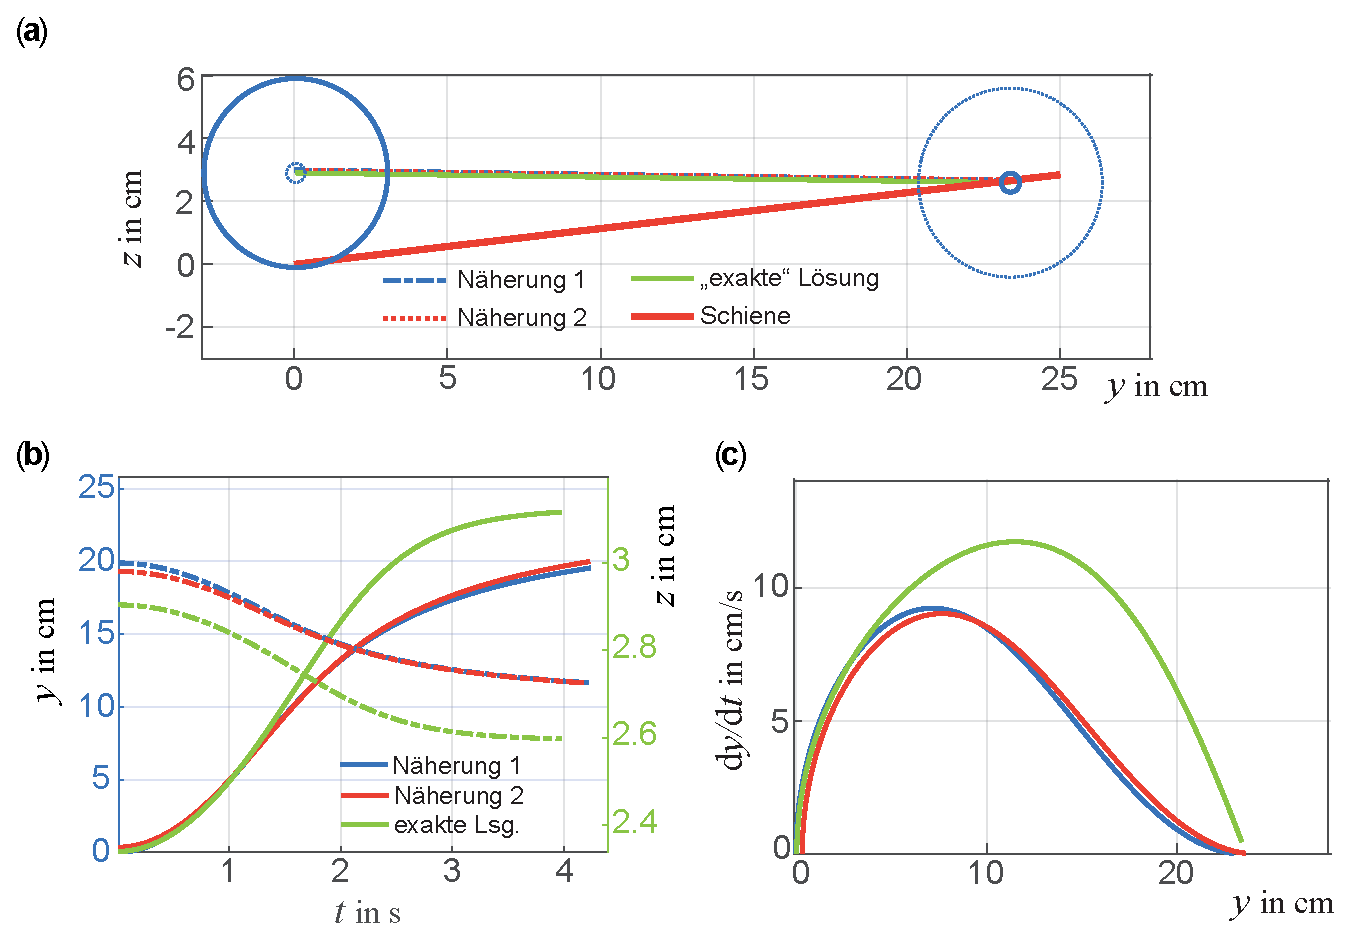
\includegraphics[width=\textwidth]{Doppelkegel10.pdf}
  \caption[Vergleich der Dynamik des aufw�rts rollenden Doppelkegels.]{Vergleich der Methoden zur Berechnung der Dynamik des aufw�rts rollenden Doppelkegels.
  a) Aufw�rtsrollen in der Geometrie. Alle drei Methoden geben ann�hernd das gleiche Bild.
  b) In der Zeitdynamik offenbaren sich die unterschiedlichen Ergebnisse.
  Der unterschiedliche $z$-Startpunkt bei der exakten L�sung resultiert aus der Tatsache, dass der Rollpunkt nicht genau unter der Symmetrieachse liegt.
  c) Noch deutlicher werden die Unterschiede in der Phasenraumdarstellung.
  Siehe \mlbewref{Doppelkegel02.m}, \mlbewref{Doppelkegel05.m}, \mlbewref{Doppelkegel06.m} und \mlbewref{DoppelkegelVergleich.m}.}\label{abb:bew_doublecone10}
\end{figure}

    \item [(B)] \emph{Rollpunkt im Punkt $x_\text{A}$ angenommen }\\ \\
    Wir wollen jetzt ber�cksichtigen, dass die Auflagepunkte nicht genau unter der Symmetrieachse liegen. Wir betrachten dazu \figref{bew_doublecone09}b und f�hren die neue generalisierte Koordinaten $y_\text{A}$ ein, die einen Punkt kennzeichnet, der senkrecht �ber dem Auflagepunkt des Kegels liegt und die H�he des Schwerpunktes hat, also $z_\text{A} = z_\text{S} = z$. Dann gilt:
		\begin{align}
    \begin{split}
        r\lk y_\text{A}\rk &= R - y_\text{A}\,\underbrace{\tan\phi\,\tan\psi}_{C_1} =  R - y_\text{A}\,C_1 \,,\\
        y\lk y_\text{A}\rk &= y_\text{A}\pm r\lk y_\text{A}\rk\,\sin\theta = y_\text{A}\,\underbrace{\lk 1 \mp C_1\,\sin\theta \rk}_{C_2} \underbrace{\pm R \,\sin\theta}_{C_4} = y_\text{A}\,C_2 + C_4\,\\
        z\lk y_\text{A}\rk &= y_\text{A} \underbrace{\lk \tan\theta - C_1 \cos\theta \rk}_{C_5} +  R \underbrace{\cos\theta}_{C_3} = y_\text{A}\,C_5 + R\,C_3 \,,\\
        \rightarrow ~~\dot{y}\lk y_\text{A}\rk &= \dot{y}_\text{A}\,\underbrace{\lk 1 \pm C_1\,\sin\theta \rk}_{C_2} = \dot{y}_\text{A}\,C_2 \, \\
        \rightarrow ~~\dot{z}\lk y_\text{A}\rk &= \dot{y}_\text{A}\,C_5\,. \label{eq:bew_lsgdcone04}
    \end{split}
    \end{align}

    Jetzt brauchen wir noch $\omega\lk y_\text{A},\dot{y}_\text{A}\rk$, welches wir wieder aus der Rollbedingung gewinnen. Wir finden:
    \begin{align}
    \begin{split}
        \alpha\lk y_\text{A}\rk &= \frac{y_\text{A}}{C_3\,\lk R-y_\text{A}\,C_1\rk} \,,\\
        \rightarrow ~~\omega\lk y_\text{A},\dot{y}_\text{A}\rk &= \dot{\alpha}\lk y_\text{A}, \dot{y}_\text{A}\rk = \frac{\dot{y}_\text{A}}{C_3\,\lk R-C_1\,y_\text{A}\rk}\,\lk 1 + \frac{C_1\,y_\text{A}}{R-C_1\,y_\text{A}}\rk \,. \label{eq:bew_lsgdcone06}
    \end{split}
    \end{align}
    Wir erhalten damit eine Lagrange-Funktion in der generalisierten Koordinate $y_\text{A}$, die weniger anschaulich ist als die Schwerpunktskoordinate $y =x_\text{S}$. �ber \eqref{eq:bew_lsgdcone04} lassen sich nat�rlich aus $y_\text{A},\, \dot{y}_\text{A}$ jederzeit $y$ und $z$ des Schwerpunktes berechnen. Die neue Lagrange-Funktion ist leider auch nicht �bersichtlicher und wir schreiben deshalb mit Abk�rzungen:
    \begin{align}
    \begin{split}
        \mathcal{L}\lk y_\text{A}, \dot{y}_\text{A} \rk &= \frac{1}{2}\,m\,\dot{y}^2\lk \dot{y}_\text{A}\rk + \frac{1}{2}\,m\,\dot{z}^2\,\lk \dot{y}_\text{A}\rk + \frac{1}{2}\,J\,\omega^2\lk y_\text{A},\dot{y}_\text{A}\rk -U\lk y_\text{A}\rk \,,\\
        T&= \frac{1}{2}\,m\,{\dot{y}_\text{A}}{}^2\,C_2{}^2 + \frac{1}{2}\,m\,{\dot{y}_\text{A}}{}^2\, C_5{}^2 \\
        &~~~+\frac{1}{2}\,m\,{\dot{y}_\text{A}}{}^2\,\lk \frac{J}{m\,C_3{}^2\,\lk R-C_1\,y_\text{A}\rk^2}\lk 1+ \frac{C_1\,y_\text{A}}{\lk R-C_1\,y_\text{A}\rk}\rk^2\rk \\
        &= \frac{1}{2}\,m\,{\dot{y}_\text{A}}{}^2\,\lek A + B + \frac{C}{\lk D-y_\text{A}\rk^2}\,\lk 1+\frac{y_\text{A}}{\lk D-y_\text{A}\rk}\rk^2\rek \,,\\
        U &= m\,g\,z = m\,g\,\lk C_3\,R + C_5\,y_\text{A}\rk \,.\label{eq:bew_lsgdcone07}
    \end{split}
    \end{align}
		
	  wobei wir f�r die numerischen Rechnungen die Abk�rzungen 
    \begin{align*}
				A &= C_2{}^2 \,,~~ B= C_5{}^2\,,~~C= \frac{J}{m\,C_3{}^2\,C_1{}^2}\,~~\text{und}~~D = \frac{R}{C_1} 
    \end{align*}
		eingef�hrt haben.

    Auch hier bleibt uns nichts anderes �brig, als die numerische L�sung anzugehen, wobei die Lagrange-Gleichung f�r $\ddot{y}$ noch komplexer wird. F�r den Phasenraum k�nnen wir aus der Energieerhaltung wieder einfach (mit $E_0 = 0 $) ableiten:
		\begin{align*}
    \begin{split}
		  \dot{y_\text{A}}(y_\text{A}) = \sqrt{\frac{-2g\,\lk C_3\,R + C_5\,y_\text{A}\rk}{ A+B+ \frac{C}{\lk D-y_\text{A}\rk^2}\,\lk 1+\frac{y_\text{A}}{\lk D-y_\text{A}\rk}\rk^2}}\,.
    \end{split}
    \end{align*}
    Aus \eqref{eq:bew_lsgdcone04} kann man sich dann entsprechend $\dot{y}(y_\text{A}), \,y(y_\text{A})\,$ usw. beschaffen. \\
		
    Die L�sungen nach den beiden Lagrange-Funktionen \eqref{eq:bew_lsgdcone03} und \eqref{eq:bew_lsgdcone07} haben wir mit der in Kapitel \ref{kap:bew_doublecone} verglichen und finden doch erhebliche Abweichungen (\figref{bew_doublecone10}), die vor allem in der inkorrekten Annahme der Lage des Rollpunktes begr�ndet sind. Obwohl die hier in der L�sung vorgestellte Vorgehensweise �ber die Lagrange-Gleichung im kartesischen Koordinaten des Schwerpunktes v�llig legitim ist, wird einmal mehr deutlich, wie kleinste Abweichungen in der Modellannahme zu deutlichen L�sungsabweichungen f�hren k�nnen und wie wichtig die richtige Wahl der generalisierten Koordinate ist. In unserem Fall hatten wir in Kapitel \ref{kap:bew_doublecone} im Fall des Doppelkegels die offensichtlich vorteilhafte Koordinate $q$ gew�hlt. Dabei ist es gar nicht so �berraschend, dass die $y$-$z$-Darstellung der N�herungen kaum vom exakten Resultat abweicht. Daf�r ist die Abweichung in der Geometrie tats�chlich klein und die N�herungen sind brauchbar. Das sind sie aber offensichtlich nicht mehr f�r die Rollbedingung und damit f�r den Anteil der Rotationsenergie. Wenn man in Kap.~\ref{kap:bew_doublecone} die \figref{bew_doublecone05} anschaut, so sieht man, dass der Radius, der gerade abrollt (am Auflagepunkt P vorliegt) gr��er ist als bei den beiden Annahmen, die wir hier in der �bung behandelt haben.  Das hei�t aber f�r die Rollbedingung, dass bei einer gegebenen Translationsgeschwindigkeit in der exakten L�sung eine kleinere Winkelgeschwindigkeit vorliegt. Folglich geht mehr Energie in die Translation, die Translationsgeschwindigkeit ist h�her und der Doppelkegel kommt schneller an sein Ziel. Genau das sieht man \figref{bew_doublecone10} sehr sch�n. Wir merken uns f�r das Vorgehen bei der Behandlung mechanischer Probleme des starren K�rpers:
\begin{enumerate}
	\item Die vorliegende Geometrie will sehr gut verstanden und im Detail analysiert sein. 
	\item F�r die Rollbedingung ist die Exaktheit sehr wichtig, denn minimale N�herungen der Lagebeschreibung des Schwerpunkts f�hren zu einer gro�en Auswirkung auf die Rollbedingung und damit �ber die Zeit zu unterschiedlichen Verh�ltnissen von Rotations- und Translationsenergie.
\end{enumerate}
		
\end{enumerate}

\end{sol} 
%\href{PhysikUncut_Part1.pdf#prb:bew_doubleconecomp}{\textcolor{blue} {$\rightarrow$ zur \probref{bew_doubleconecomp}.}}\\
\textcolor{blue} {$\rightarrow$ zur} \probref{bew_doubleconecomp}.\\
\noindent\rule[1ex]{\textwidth}{0.5pt}  

%-----------------------------------------------------------------------------------------------------------
\newpage
\hypertarget{lsg:bew_TrainTrack}{}
\begin{sol}{prob:bew_TrainTrack}\label{lsg:bew_TrainTrack} %�bung54
\textbf{Stabilit�t von starren Radachsen auf Schienen} \\ 
\begin{enumerate}
    \item [1)] \textit{Dynamische Ableitung des Sinus-Laufs} \\
		
In \figref{bew_TrainWheel04a}b haben wir f�r die laterale St�rung auch das Kr�ftediagramm dargestellt. In dem Doppelkegel-Modell k�nnen wir daraus die Bewegungsgleichung f�r den Schwerpunkt aufschreiben:
\begin{align}
\begin{split}
    m\,\ddot{x}_\text{S} &= -F_\text{NL}\,\sin\lk\psi-\theta\rk+F_\text{NR}\,\sin\lk\psi+\theta\rk \,,\\
    m\,\ddot{z}_\text{S} &= F_\text{NL}\,\cos\lk\psi-\theta\rk+F_\text{NR}\,\cos\lk\psi+\theta\rk-m\,g \,.
\end{split}\label{eq:bew_TrainWheel01}
\end{align}

\begin{figure}
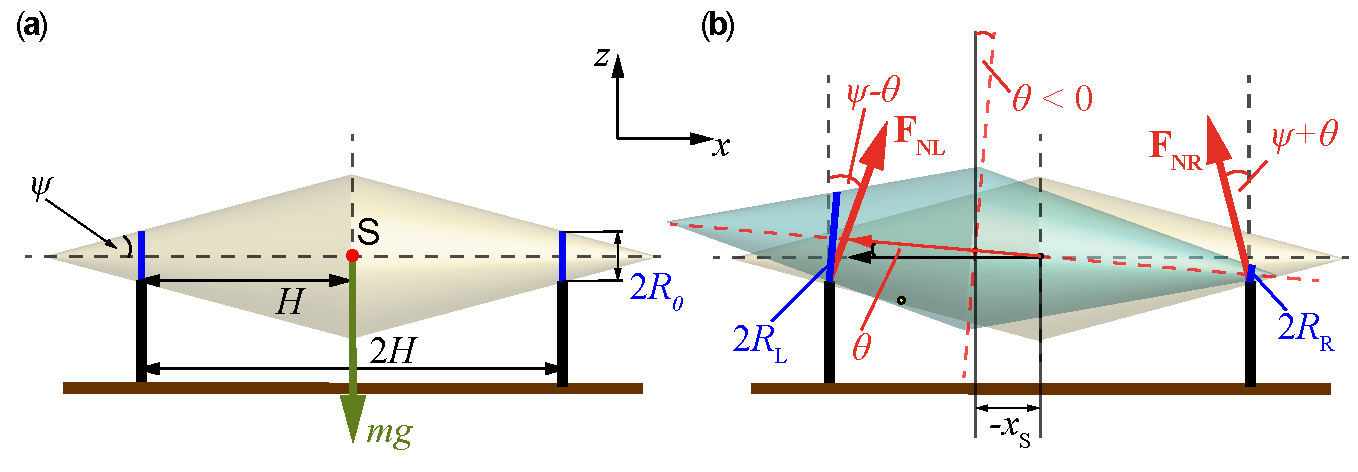
\includegraphics[width=\textwidth]{LateraleStoerung.pdf}%
\caption[Laterale St�rungen auf eine starre Radachse auf einer Doppelschiene.]{Laterale St�rungen auf eine Radachse auf einer Doppelschiene (Modellansicht von hinten in Fahrtrichtung). \fa Normallage der Radachse, $2H$ ist die Spurbreite, $\gamma$ die Konizit�t der Radform, $R_0$ ist der Rollradius in der Normallage und S der Schwerpunkt der Achse, $m$ die Gesamtmasse von Achse und Achslast. \fb Lage bei lateraler St�rung und wirkende Normalkr�fte. $x_\text{S}$ ist die laterale Verschiebung des Schwerpunktes, $\theta$ der resultierende Kippwinkel auf Grund der Konizit�t, $\vec{F}_\text{N}$ die von der Schienenauflage ausgehenden Normalkr�fte und $R_\text{L}, R_\text{L}$ die neuen resultierenden Rollradien auf dem linken \bzw rechten Auflagepunkt. Der Winkel $\theta$ ist im eingezeichneten Fall negativ.} \label{abb:bew_TrainWheel04a}
\end{figure}

Man beachte, dass wir hier nur die Normalkr�fte (Auflagekr�fte) $F_\text{N}$ ber�cksichtigt haben und der Winkel $\theta$ aus der durch die komische Form folgende Verkippung des Radsatzes infolge der lateralen St�rung resultiert. Ebenfalls sei auf die Asymmetrie in den beiden Gleichungen infolge der Wirkung der Gravitation hingewiesen. Wir brauchen noch eine Gleichung f�r den Winkel $\theta$, der unsere dritte generalisierte Koordinate darstellt. Unter der Ber�cksichtigung, dass das Tr�gheitsmoment $J_x$ sehr viel kleiner als das Tr�gheitsmoment $J_y$ ist (da f�r $J_y$ noch die gesamte Masse des Wagens etc. ber�cksichtigt werden muss), kann man die Bewegungsgleichung f�r $\theta$ n�herungsweise wie folgt aufschreiben:
\begin{align}
\begin{split}
    J_y\,\ddot{\theta} = &\sum_i\,\lk M_i\rk_y = \sum\,\lk \vec{r}_i\times \vec{F}_i\rk_y \\
    = &R_0\,\lek F_\text{NL}\,\sin\lk\psi-\theta\rk - F_\text{NR}\,\lk \psi+\theta\rk\rek - \lk H-x_\text{S}\rk\,F_\text{NL}\,\cos\lk\psi-\theta\rk \\
    &+ \lk H+x_\text{S}\rk\,F_\text{NR}\,\cos\lk\psi+\theta\rk\,.
\end{split} \label{eq:bew_TrainWheel02}
\end{align}
Dieses verkoppelte nichtlineare DGL-System k�nnten wir ohne weiteres numerisch l�sen. Wir wollen aber eine Linearisierung versuchen, und zwar unter der Annahme, das $x_\text{S}, z_\text{S}$ und $\theta$ nur kleine St�rungen von der Nulllage darstellen. Wir sind ja gerade an einer stabilen L�sung interessiert, die notwendigerweise $x_\text{S}, z_\text{S}$ und $\theta$ begrenzt halten muss. Ferner sei der konische Winkel $\psi$ ebenfalls klein. Mit der N�herung $z_\text{S}\approx 0$, $\tan\psi/H\approx \psi/H$ folgt
\begin{align}
    \theta = -\frac{\tan\psi}{H}\,x_\text{S} \approx -\psi\,\frac{x_\text{S}}{H}\label{eq:bew_TrainWheel03}
\end{align}
und aus \eqref{eq:bew_TrainWheel01} bzw. \eqref{eq:bew_TrainWheel02}
    \begin{subequations}
    \begin{align}
    m\,\ddot{x}_\text{S} &= -F_\text{NL}\,\lk \psi+\psi\,\frac{x_\text{S}}{H}\rk + F_\text{NR}\,\lk\psi - \psi\,\frac{x_\text{S}}{H}\rk \notag \\
		                     &= \psi\,\lek -F_\text{NL}\,\lk 1 + \frac{x_\text{S}}{H}\rk + F_\text{NR}\,\lk 1-\frac{x_\text{S}}{H}\rk\rek \,, \\
    0 &=F_\text{NL} + F_\text{NR} -m\,g   \,, \\
    J_y\,\ddot{\theta} &= -J_y\,\frac{\psi}{H}\,\ddot{x}_\text{S} = -m\,R_0\,\ddot{x}_\text{S}-\lk H-x_\text{S}\rk\, F_\text{NL} + \lk H+x_\text{S}\rk\, F_\text{NR}\,. \label{eq:bew_TrainWheel04}
    \end{align}
    \end{subequations}
Aus diesen Gleichungen kann man die unbekannten Normalkr�fte $F_\text{NL}, F_\text{NR}$ eliminieren und wir erhalten eine Bewegungsgleichung f�r die Schwerpunktkoordinate $x_\text{S}$:
\begin{align}
    \underbrace{\frac{1}{2m\,g}\lk J_y\,\frac{\psi}{H} - m\,R_0 + \frac{m\,H}{\psi}\rk}_{1/\omega_\text{S}{}^2}\,\ddot{x}_\text{S} + x_\text{S} = 0  \,. \label{eq:bew_TrainWheel07}
\end{align}
Da $R_0<\frac{\psi}{H}\,\frac{J_y}{m}$ und $R_0<\frac{H}{\psi}$ ist die Klammer in \eqref{eq:bew_TrainWheel07} positiv und die Bewegungsgleichung ist eine Schwingungsgleichung mit der Frequenz $\omega_\text{S}$. Damit bleibt $\ddot{x}_\text{S}$ begrenzt und die Radachse zeigt einen Sinuslauf. Die Frequenz $\omega_\text{S}$ ist gegeben durch:
\begin{align*}
    \omega_\text{S} = \sqrt{\frac{2g}{\frac{J_y}{m}\,\frac{\psi}{H} - R_0 + \frac{H}{\psi}}}
\end{align*}
und f�r ein $J_y \approx C\,m\,H^2$ worin $C$ je nach Aufbau der Achse und Beladung eine dimensionslose Konstante in der Gr��enordnung von $1-10$ ist, ergibt sich
\begin{align}
    \omega_\text{S} = \sqrt{\frac{2g}{C\,\psi\,H - R_0 + H/\psi}}\,.  \label{eq:bew_TrainWheel08}
\end{align}
Die Sinuslauf-Frequenz $\omega_\text{S}$ f�r $x_\text{S}(t)$ als Funktion von $\psi$ ist in \figref{bew_TrainWheel05}a gezeigt.\footnote{In Kap. \ref{kap:bew_traintracks} haben wir eine alternative kinematische Ableitung (auch anwendbar f�r beliebige Radprofile) behandelt. Dort hatten wir eine Beziehung f�r $x_\text{S}(y_\text{S})$ hergeleitet, mit der Frequenz $\omega_\text{K}$. Hier haben wir eine Beziehung f�r $x_\text{S}(t)$ hergeleitet, mit der Frequenz $\omega_\text{S}$. Zwischen beiden Frequenzen sollte n�herungsweise $\omega_\text{S} = v_0\,\omega_\text{K}$ gelten, was aber nicht der Fall ist. Die aus dem dynamischen Modell abgeleitete Frequenz ist deutlich kleiner und der Rollradius taucht in der Formel f�r $\omega_\text{S}$ gar nicht auf, daf�r der Faktor $g$, wie f�r ein dynamisches Modell mit Massen zu erwarten war. Daraus kann man m�glicherweise die Schlussfolgerung ziehen, dass die wesentliche Stabilit�t bei Geradeauslauf von den unterschiedlichen Rollradien bestimmt wird.}

\begin{figure}
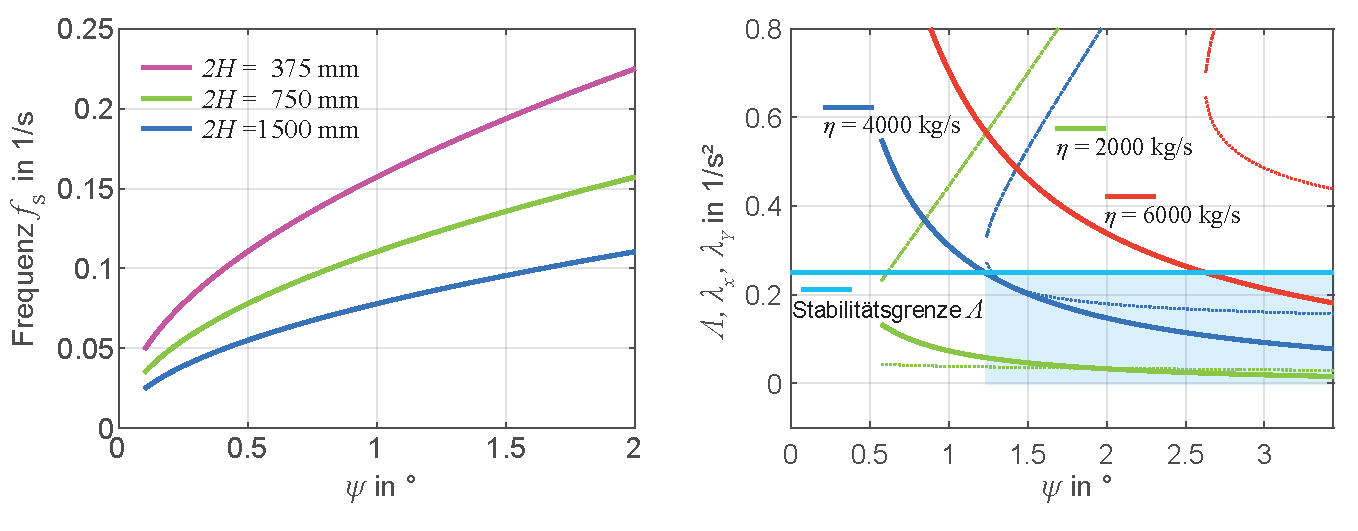
\includegraphics[width=\textwidth]{RadachsenStabilitaet.pdf}
\caption[Berechnung der dynamischen Stabilit�t von starren Radachsen.]{Berechnung der dynamischen Stabilit�t von starren Radachsen.
a) Frequenz des Sinuslaufs als Funktion der Konizit�t.
b) Stabilit�tsdiagramm f�r starre Achsen auf Schienen unter Ber�cksichtigung von Lenkfehlern.
Parameter: Schienenbreite $2H = \SI{1.435}{\metre}$, Rollradius $R_0 = \SI{0.487}{\metre}$, Geschwindigkeit $v_0 = \SI{50.0}{\metre\per\second}$, Masse $m = \SI{45e3}{\kg}$, Tr�gheitsmoment $J_z = \SI{2.27e06}{\kg\metre\squared}$, Tr�gheitsmoment $J_y = \SI{0.26e06}{\kg\metre\squared}$, Reibungskoeefizient $\eta = \SI{4.0e03}{\kg\per\second}$.
Siehe auch \mlbewref{Sinuslauf.m}.}
\label{abb:bew_TrainWheel05}
\end{figure}

		%Item2
    \item [2)] \textit{Ber�cksichtigung von Lenkfehlern} \\
    Wir wollen nun Lenkfehler (\figref{bew_TrainWheel07}), also zus�tzlich eine �nderung um den Lenkwinkel $\varphi$, ber�cksichtigen und m�ssen dabei auch die Reibung zwischen Schiene und Rad in Betracht ziehen. In der N�herung kleiner Winkel gilt zun�chst weiterhin nach \figref{bew_TrainWheel04} 
		
\begin{figure}
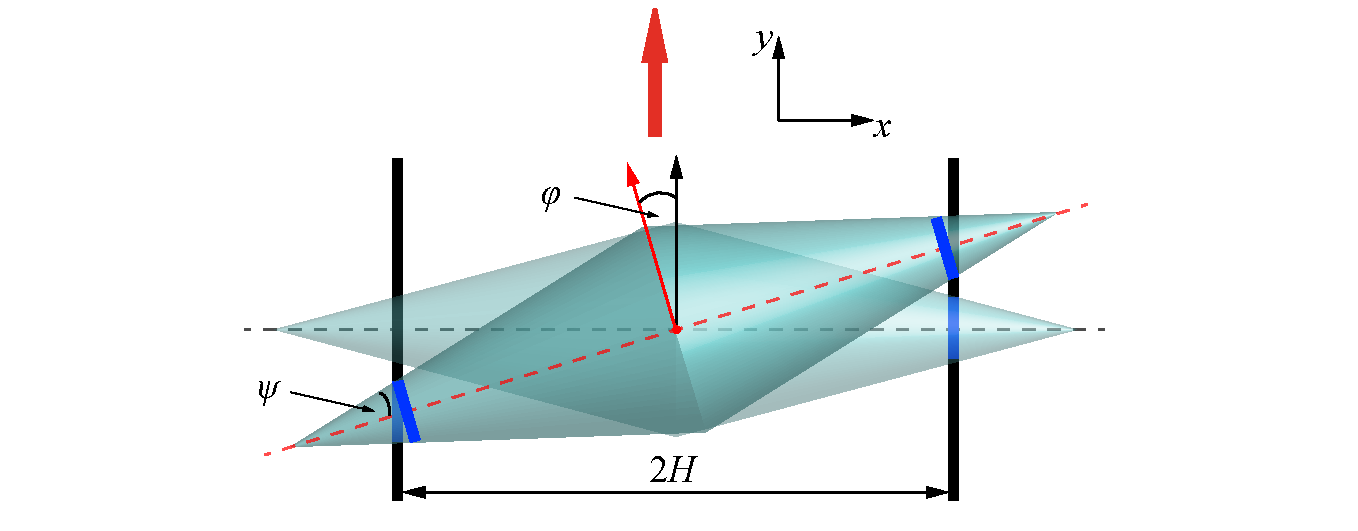
\includegraphics[width=\textwidth]{TrainWheelTopView.pdf}%
\caption[Lenkfehler bei starren Radachsen]{Lenkfehler bei starren Radachsen} \label{abb:bew_TrainWheel07}
\end{figure}

    \begin{align}
    \begin{split}
        \vec{F}_\text{NL} &= F_\text{NL}\,\vec{e}_z - \lk \psi-\theta\rk\,F_\text{NL}\,\vec{e}_x \,, \\
        \vec{F}_\text{NR} &= F_\text{NR}\,\vec{e}_z - \lk \psi+\theta\rk\,F_\text{NR}\,\vec{e}_x \,.
    \end{split}  \label{eq:bew_TrainTrack08}
    \end{align}
    Um die Reibungskr�fte berechnen zu k�nnen, brauchen wir die Rollgeschwindigkeiten. Wir wollen weiterhin reines Rollen annehmen, dann gilt 
    \begin{align}
    \begin{split}
        v_\text{L} = &-v\,\vec{e}_y + \dot{x}_\text{S}\,\vec{e}_x + \omega\,\lk R_0 + x_\text{S}\,\tan\psi\rk\,\vec{e}_y \\
        &-\varphi\,\omega\,\lk R_0 + x_\text{S}\,\tan\psi\rk\,\vec{e}_x + \lk H-x_\text{S}\rk\,\dot{\varphi}\,\vec{e}_y \,, \\
        v_\text{R} = &-v\,\vec{e}_y + \dot{x}_\text{S}\,\vec{e}_x + \omega\,\lk R_0 - x_\text{S}\,\tan\psi\rk\,\vec{e}_y \\
        &-\varphi\,\omega\,\lk R_0 - x_\text{S}\,\tan\psi\rk\,\vec{e}_x - \lk H+x_\text{S}\rk\,\dot{\varphi}\,\vec{e}_y\,.
    \end{split}\label{eq:bew_TrainTrack09}
    \end{align}
    Wir machen die N�herung, dass $v = v_0= \text{const.}$ und $\omega=\omega_0 = \text{const.}$, d.h. dass die Vorw�rtsgeschwindigkeit $v_0$ des Zuges und die Rollfrequenz der Radachse $\omega_0$ konstant sind und durch die St�rungen nicht (bzw. nur sehr gering) beeinflusst werden. Ferner wvernachl�ssigen wir Produkte von kleinen Gr��en, also z.\,B. $x_\text{S} \dot\varphi$. Dann wird aus \eqref{eq:bew_TrainTrack09} bei kleinen Winkeln:
    \begin{align}
    \begin{split}
        v_\text{L} &= \dot{x}_\text{S}\,\vec{e}_x + \omega_0\,\psi\,x_\text{S}\,\vec{e}_y - \omega_0\,R_0\,\varphi\,\vec{e}_x +H\,\dot{\varphi}\,\vec{e}_y \,, \\
        v_\text{R} &= \dot{x}_\text{S}\,\vec{e}_x - \omega_0\,\psi\,x_\text{S}\,\vec{e}_y - \omega_0\,R_0\,\varphi\,\vec{e}_x -H\,\dot{\varphi}\,\vec{e}_y \,.
    \end{split}\label{eq:bew_TrainTrack10}
    \end{align}
    Wir k�nnten nun mit $v_\text{L}$, $v_\text{R}$ aus \eqref{eq:bew_TrainTrack10} die Reibungskr�fte $F_\text{RL}$, $F_\text{RR}$ berechnen, wollen aber zuvor \eqref{eq:bew_TrainTrack10} noch weiter vereinfachen und die Terme mit den Ableitungen von $\dot{x}$ und $\dot{\varphi}$ nicht mitnehmen, da wir ja an einer stabilen Schwingungsl�sung f�r $x$, $\varphi$ interessiert sind und daher das System durch $x\lk t\rk$ und $\varphi\lk t\rk$ bestimmt wird. Damit erhalten wir f�r die Reibungskr�fte $F_\text{RL} = -\eta \,v_\text{L}$ bzw. $F_\text{RR} = -\eta\,v_\text{R}$ die folgende Beziehung:\footnote{Die Frage, ob die Reibung hier zur Geschwindigkeit proportional nach $F\propto\eta\,v$ ist oder eher einer Gleitreibung nach $F\propto \mu\,F_\text{N}$ entspricht, ist v�llig berechtigt. Die Annahme $F\propto \mu\,F_\text{N}$ l�sst sich sehr einfach in unserem Modell behandeln und wird dem Leser als �bung empfohlen.}
    \begin{align}
    \begin{split}
        F_\text{RL} &= -\eta\,\psi\,\omega_0\,x_\text{S},\vec{e}_y + \eta\,\omega_0\,R_0\,\varphi\,\vec{e}_x \,,\\
        F_\text{RR} &= +\eta\,\psi\,\omega_0\,x_\text{S},\vec{e}_y + \eta\,\omega_0\,R_0\,\varphi\,\vec{e}_x \,,
    \end{split} \label{eq:bew_TrainTrack11}
    \end{align}
    worin $\eta$ ein Reibungskoeffizient ist. Mit \eqref{eq:bew_TrainTrack08} und \eqref{eq:bew_TrainTrack11} haben wir alle Kr�fte des Systems bestimmt. Wir brauchen noch die Ortsvektoren $\vec{r}_\text{L}$ und $\vec{r}_\text{R}$
    \begin{align}
    \begin{split}
        \vec{r}_\text{L} &= \lk H-x_\text{S}\rk\,\vec{e}_x + h\,\varphi\,\vec{e}_y - R_0\,\vec{e}_z\,, \\
        \vec{r}_\text{R} &= \lk H+x_\text{S}\rk\,\vec{e}_x - h\,\varphi\,\vec{e}_y - R_0\,\vec{e}_z\,,
    \end{split} \label{eq:bew_TrainTrack12}
    \end{align}
    um die Drehmomente auszurechnen. Dann k�nnen wir die folgenden Bewegungsgleichungen aufschreiben (Wir haben 4 Freiheitsgrade $x_\text{S}$, $z_\text{S}$, $\theta$ und $\varphi$, folglich gibt es vier Bewegungsgleichungen):
    \begin{subequations}
    \begin{align}
        m\,\ddot{z}_\text{S} = &F_\text{NL} + F_\text{NR} -m\,g \,,\\
        m\,\ddot{x}_\text{S} = &-F_\text{NL}\,\lk \psi-\theta\rk + F_\text{NR}\,\lk \psi+\theta\rk + 2\eta\,\omega_0\,R_0\,\varphi \,,\\
        J_y\,\ddot{\theta}= &-2\eta\,\omega_0\,R_0{}^2 \,\varphi + R_0\,\lek F_\text{NL}\,\lk \psi-\theta \rk -F_\text{NR} \,\lk \psi+\theta\rk\rek \\
        &-\lk H-x_\text{S}\rk \,F_\text{NL} + \lk H+ x_\text{S}\rk\,F_\text{NR}   \nonumber \,,\\
        J_z\,\ddot{\varphi} = &-2\eta\,H\,\psi\,\omega_0\,x_\text{S} +2\,\lk F_\text{NL} +F_\text{NR}\rk\,\psi\,H\,\varphi  \,. \label{eq:bew_TrainTrack13}
    \end{align}
    \end{subequations}
    Wir k�nnen wieder die Normalkr�fte eliminieren und erhalten ein gekoppeltes DGL-System 2. Ordnung aus zwei Gleichungen
    \begin{subequations}
    \begin{align}
        Q\,\ddot{x}_\text{S} &= -2m\,g\,x_\text{S} + 2\eta\,\frac{H\,\omega_0\,R_0}{\psi}\,\varphi\,,\\
        J_\text{z}\,H\,\ddot{\varphi} &= -2m\,H^2\,\psi\,\omega_0\,x_\text{S} + 2m\,g\,H^2\,\psi\,\varphi \,, \label{eq:bew_TrainTrack14}
    \end{align}
    \end{subequations}
    worin $Q = J_\text{y}\,\frac{\psi}{H} - m\,R_0 +\frac{m\,H}{\psi} = 2m\,g\,/\omega_\text{S}{}^2\,$ ist (\vgl auch \eqref{eq:bew_TrainWheel08}). \\
    Wenn wir beide Gleichungen in einer L�ngendimension schreiben, dann ergibt sich mit $Y = H\,\varphi$ 
    \begin{align}
        \begin{pmatrix}
            \ddot{x}_\text{S} \\
            Y
        \end{pmatrix}
        = 
        -\begin{pmatrix}
            +\frac{2m\,g}{Q} & -\frac{2\eta\,\omega_0\,R_0}{\psi\,Q} \\
            +\frac{2\eta\,H^2\,\psi\,\omega_0}{J_\text{z}} & -\frac{2m\,g\,H\,\psi}{J_\text{z}}
        \end{pmatrix}
        \,\begin{pmatrix}
            x_\text{S}\\
            Y
        \end{pmatrix}
				\,, \label{eq:bew_TrainTrack15}
    \end{align}
    oder kurz
    \begin{align*}
        \ddot{\hat{X}} = -\mathbb{M}\,\hat{X}\,.
    \end{align*}
    Die Frage ist nun, wann es f�r \eqref{eq:bew_TrainTrack15} stabile, also in $\hat{X}$ begrenzte L�sungen gibt. Dazu bestimmen wir die Eigenwerte der Matrix $\mathbb{M}$ �ber
    \begin{align}
        \ddot{\hat{X}} = -
        \begin{pmatrix}
            \lambda_x &0\\
            0 & \lambda_Y
        \end{pmatrix}\,
        \hat{X} \,.\label{eq:bew_TrainTrack16}
    \end{align}
    Damit das System stabil bleibt, m�ssen beide Eigenwerte $\lambda_x$, $\lambda_Y$ positiv sein, d.h. 
    \begin{align}
        \lambda_{x,Y} = \frac{1}{2}\,\lk \mathcal{T} \pm \sqrt{\mathcal{T}^2 -4\mathcal{D}} \rk > 0 \label{eq:bew_TrainTrack17}
    \end{align}
    worin 
    \begin{align*}
        \mathcal{T} &= \mathbb{M}_{11} + \mathbb{M}_{22} ~~~~\text{die Spur von}~~\mathbb{M}~~\text{ und }\\
        \mathcal{D} &= \mathbb{M}_{11}\,\mathbb{M}_{22} - \mathbb{M}_{21}\,\mathbb{M}_{12}~~~~\text{ die Determinante von} ~~\mathbb{M}~~\text{ ist.}
    \end{align*}
    Aus \eqref{eq:bew_TrainTrack17} folgt:
    \begin{align}
        0 < \frac{\mathcal{D}}{\mathcal{T}^2} < \frac{1}{4} \,.\label{eq:bew_TrainTrack18}
    \end{align}
   \figref{bew_TrainWheel05}b zeigt, das Stabilit�tsdiagramm $\lambda_x - \lambda_Y$ als Funktion der Parameter $\psi$ und $\eta$. Man erkennt, das es in jedem Fall der Stabilit�t dient, wenn $\mathcal{T}$ gro� wird, was durch gro�e Spurbreiten $2H$, sowie einen entsprechenden minimalen Konizit�tswinkel $\psi$ (f�r den Parametersatz mit $ \eta = \SI{4.0e03}{\kg\per\second}$ blau schattiert eingezeichnet) erreicht werden kann.\\

\begin{nebenrechnung}{Nebenrechnung:}
~~Berechnung der Spur und Determinante:
     \begin{align*}
         \mathcal{T} &= \mathbb{M}_{11} + \mathbb{M}_{12}= -\frac{2m\,g}{Q}\,\lk 1+\frac{H\,\psi\,Q}{J_z} \rk = - \omega_\text{S}{}^2 \,\lk 1+\frac{2m\,g\,H\,\psi}{J_z\,\omega_\text{S}{}^2}\rk \\
         \mathcal{D} &= \mathbb{M}_{11}\,\mathbb{M}_{22} - \mathbb{M}_{21}\,\mathbb{M}_{12} = \frac{2m^2\,g^2\,\omega_\text{S}{}^2}{J_\text{z}} \lk 1  + \frac{2\eta^2\,H^2\,\omega_0{}^2\,R_0}{m\,g\,\psi\,J_\text{z}} \rk 
 \end{align*}
\end{nebenrechnung}

\textbf{Bemerkung:}\\ \\
Der aufmerksame Leser hat sicher festgestellt, dass die Frequenz 
	\[\omega_\text{S} = \sqrt{\frac{2g}{C\,\psi\,H - R_0 + H/\psi}}
	\]
nach Gleichung \eqref{eq:bew_TrainWheel08} sich von der Frequenz 
	\[\omega_\text{K} = 2\pi\,f_\text{K} = \frac{v_0}{2\pi}\,\sqrt{\frac{\psi}{H\,R_0}}
	\]
nach Gleichung \eqref{eq:bew_TrainTrack07} unterscheidet.
Dies kann man man wie folgt verstehen. Schaut man sich die Beziehung \eqref{eq:bew_TrainTrack04} bzw. \eqref{eq:bew_TrainTrack06} aus Kapitel \ref{kap:bew_traintracks} an, so hat man den station�ren Teil einer Wellengleichung vor sich (siehe Kap.\ \ref{chap:kontmech}. Diese Wellengleichung muss nat�rlich auch dynamisch zu gewinnen sein. Auff�llig ist, dass in dieser Wellengleichung in Kapitel \ref{kap:bew_traintracks} kein Einfluss der Gravitation zu sehen ist ($g$ ist nicht enthalten), jedoch in der dynamischen Herleitung, die zur Beziehung \eqref{eq:bew_TrainWheel08} f�r $\omega_\text{S}$ f�hrt, was auf Grund des Ansatzes mit den Normalkr�ften auch zu erwarten ist. Tats�chlich ben�tigt man f�r die Herleitung der Beziehung \eqref{eq:bew_TrainTrack07} die Gravitation nicht als r�cktreibende Kraft. Sie hat hier nur daf�r zu sorgen, dass immer Kontakt zwischen den Schienen und R�dern besteht. Die Ursache f�r die r�cktreibende Kraft in der Herleitung von Beziehung \eqref{eq:bew_TrainTrack07} f�r 
$\omega_\text{K}$ deutet sich in Gleichung \eqref{eq:bew_TrainTrack02} an. Um die (durch die Achse erzwungene) als konstant angenommene Winkelfrequenz f�r beide R�der zu erreichen, werden Reibungskr�fte erzwungen, die das entsprechende Drehmoment um die $z$-Achse aufbringen m�ssen. F�r eine dynamische Herleitung f�r denselben Effekt m�sste man daher die inneren Kr�fte in der Achse und der Reibung ansetzen, die aber im Allgemeinen unbekannt sind.\\
Anders herum wird in der �bung eigentlich f�r die Herleitung von \eqref{eq:bew_TrainTrack08} die Bewegung in $y$-Richtung f�r den ersten Teil ohne Lenkfehler nicht ben�tigt. Der Zug k�nnte diese Schwingungsbewegung aufgrund der Schwerpunktverlagerung und der r�cktreibenden Gravitation auch im Stand durchf�hren (wenn er denn die Haftreibung �berwinden k�nnte). Die Frequenz h�ngt daher nicht von der Geschwindigkeit ab, das muss dann aber zwangsweise die Wellenl�nge.\\
Zusammengefasst kann man sagen, die unterschiedlichen Frequenzen $\omega_\text{K}$ und $\omega_\text{S}$ ergeben sich aus der Betrachtung unterschiedlicher physikalischer Effekte.

\end{enumerate}
\end{sol} 
%\href{PhysikUncut_Part1.pdf#prb:bew_TrainTrack}{\textcolor{blue} {$\rightarrow$ zur \probref{bew_TrainTrack}.}}\\
\textcolor{blue} {$\rightarrow$ zur} \probref{bew_TrainTrack}.\\
\noindent\rule[1ex]{\textwidth}{0.5pt}  \newpage

%-----------------------------------------------------------------------------------------------------------
\newpage
\hypertarget{lsg:bew_gyrotwister}{}
\begin{sol}{prob:bew_gyrotwister}\label{lsg:bew_gyrotwister} %�bung55
\textbf{Gyrotwister als Trainingsger�t} \\ \\
Um bestimmen zu k�nnen, welche Kr�fte hier wirken, ben�tigen wir zun�chst
das Tragheitsmoment des Kreisels. Da wir ihn als Vollkugel annehmen m�chten,
berechnet sich dieses zu
\begin{equation*}
  J = \frac{2}{5} m R^2 = \frac{2}{5} \cdot \SI{0.25}{\kilo\gram} \cdot
  \left (\SI{0.025} {\metre}\right)^2 =  \SI{6.25e-5}{\kilo\gram\, \metre^2}
  \; .
\end{equation*}

Das Drehmoment, das n�tig ist, um die schnelle Rotation zu �ndern, wenn
wir die Hand fest halten und nicht gerade weiter beschleunigen, ergibt
sich aus Gleichung \eqref{eq:bew_gyrotwo_M0} mit $\hat{\Omega}_\text{H} = 0$ und $J_3 = J$.
Es lautet mit $\omega'_1 = \Omega_\text{U} = \SI{40}{\per\second}$ und $\omega'_3 = \Omega_\text{S} = \SI{200}{\per\second}$:
\begin{equation*}
  \left|M_0\right| = J \omega'_1 \omega'_3 = \SI{6.25e-5}{\kilo\gram\, \metre^2} \cdot
  \SI{40}{\per\second} \cdot \SI{200}{\per\second} = \SI{0.5}{\kilo\gram\,
    \metre^2\, \per s^2} \, .
\end{equation*}

Um dieses Drehmoment aufbringen zu k�nnen, muss man am Geh�use die Kraft
\begin{equation*}
  F = \frac{\left|M_0\right|}{R} = \frac{\SI{0.5}{\kilo\gram\, \metre^2\, \per s^2}}
    {\SI{0.025}{\metre}} = \SI{20}{\newton}
\end{equation*}
aufbringen. Eine Hantel der Masse
\begin{equation*}
  m = \frac{F}{g} = \frac{\SI{20}{\newton}}{\SI{9.81}{\metre\per s^2}}
  = \SI{2.02}{\kilo\gram}
\end{equation*}
k�nnte die gleiche Kraft auf den Arm aus�ben. In diesem Fall w�re also
die Hantel der Masse $m = \SI{3}{\kilo\gram}$ das effektivere Trainingsger�t.
Jedoch l�sst sich der Gyrotwister noch weiter beschleunigen, sodass er die
Hantel auch deutlich �bertreffen kann.

\end{sol} 
%\href{PhysikUncut_Part1.pdf#prb:bew_gyrotwister}{\textcolor{blue} {$\rightarrow$ zur \probref{bew_gyrotwister}.}}\\
\textcolor{blue} {$\rightarrow$ zur} \probref{bew_gyrotwister}.\\
\noindent\rule[1ex]{\textwidth}{0.5pt}  \newpage

%-----------------------------------------------------------------------------------------------------------
\hypertarget{lsg:bew_gyroskope}{}
\begin{sol}{prob:bew_gyroskope}\label{lsg:bew_gyroskope} %�bung56
\textbf{Gyroskope} \\ \\

Aufgrund der Drehimpulserhaltung weist der Kreisel ein hohes Beharrungsverm�gen gegen�ber Lage�nderungen im Raum auf. Ein freier, symmetrischer Kreisel hat das Bestreben, die Richtung seiner Drehachse im Inertialsystem beizubehalten. Damit k�nnen Kreisel sowohl als Navigationsinstrumente als auch zur aktiven Lageregelung eingesetzt werden.

Wir unterschieden folgende Anwendungen:
\begin{enumerate}
	\item \textbf{Lageregelung, Stabilisierung}\\
	Hier wird ein freier Kreisel benutzt, meist in halb- oder voll-kardanischer Aufh�ngung, \zb in der Lageregelung von Satelliten oder Schiffen. Dabei wird ausgenutzt, dass das Gesamtsystem aus Raumflugk�rper/Schiffsk�rper und Gyroskop seinen Drehimpuls beibeh�lt und somit durch Drehimpuls�bertragung zwischen beiden K�rpern die Lage des Raumschiffs/Schiffs gesteuert werden kann.\\
	
	Ausnutzung: Gesamtdrehimpulserhaltung\\
	Zahl der freien Achsen\footnote{Wir z�hlen alle nicht eingeschr�nkten Drehachsen (Eulersche Winkel) des Kreisels, also auch die Bewegung um die Drehachse/Symmetrieachse (Winkel $\psi$, die ja \ia konstant ist). Im angels�chsischen Raum wird diese Achse nicht mitgez�hlt, daher hat im dortigen Sprachgebrauch ein eingeschr�nkter Kreisel  also nur einen oder keinen Freiheitsgrad, ein nicht eingeschr�nkter Kreisel zwei.}: 2 oder 3 \\
	
	\item \textbf{Wendezeiger}\\
	Beim Wendezeiger wird ein halbkardanisch aufgeh�ngter Kreisel benutzt. Die Kreiselachse ist parallel zur Flugzeugquerachse gelagert. Die Drehachse des Rahmens ist parallel zur L�ngsachse des Flugzeugs ausgerichtet. Im Kurvenflug dreht sich das Flugzeug um die Hochachse. Dann kippt die Drehachse des Kreisels auf Grund der Pr�zession. Diese Kippbewegung, die von der Kurvengeschwindigkeit abh�ngig ist, wird durch einen Zeiger angezeigt. Das bewirkt, dass der Wendezeiger Drehungen des Flugzeugs um die Hochachse des Flugzeugs (das sogenannte Gieren) anzeigt.\footnote{Wir m�chten an dieser Stelle erw�hnen, das in einem Flugzeug mit Motor in Ausrichtung der L�ngsachse (\zb Cessna) ein symmetrischer Kreisel vorliegt. Als Konsequenz w�rde bei einem motorisierten Kurvenflug in einer Linkskurve (rechts drehender Motor angenommen) das Flugzeug eine Nickbewegung nach oben ausf�hren.\\Man benutze die Rechte-Hand-Regel $\vec{M}_\text{Nick} = \omega_\text{Kurve} \times \vec{L}_\text{Motor}$.}\\

	Ausnutzung: Pr�zession \\
	Zahl der freien Achsen: 2 \\
	
	\item \textbf{K�nstlicher Horizont}\\
   Der k�nstliche Horizont enth�lt einen vollkardanisch (mit drei Freiheitsgraden) aufgeh�ngte Kreisel, den sogenannten Horizont- oder Lotkreisel, der in seiner Lage im Inertialsystem stabil bleibt.\footnote{Der k�nstliche Horizont soll die Lage bez�glich der idealen Erdoberfl�che anzeigen. Nun sind aber Koordinaten auf der Erde kein Inertialsystem, sondern die Erde dreht sich unter dem Kreisel weg. In kleinerem Ausma� geschieht das auch, wenn das Flugzeug �ber der gekr�mmten Erdoberfl�che eine gr��ere Distanz zur�cklegt. Deshalb muss ein k�nstlicher Horizont durch einen geeigneten Lotf�hler nachgef�hrt werden.} Das Flugzeug dreht sich gewisserma�en um das Instrument, insbesondere bleibt auch der Horizontbezug aufrecht. Die Lage der Kreiselachse in Bezug zum Geh�use kann mechanische oder elektrische auf eine Anzeige �bertragen werden.
	 \\
	
	Ausnutzung: Drehimpulserhaltung freier Kreisel\\
	Zahl der freien Achsen: 3 \\
\newpage
	\item \textbf{Nordsuchender Kreiselkompass}\\
   Beim Kreiselkompass wird die Bewegung eines Gyroskops durch die Schwerkraft und eine Zwangsbedingung auf die Horizontebene eingeschr�nkt, \dh die Figurenachse bleibt immer in der Horizontebene liegen, kann sich dort aber frei drehen.\\
	 Die Rotation der Erde von W nach O f�hrt dann dazu, dass aus Sicht eines auf dem Kreisel mitbewegten und in die initiale Westrichtung schauenden Beobachters die Westseite der Horizontebene relativ zur anf�nglich auch im Erdsystem bewegungslosen Kreiselrotationsachse ansteigt, w�hrend die Ostseite absinkt. Diese �nderung der Horizontebene bewirkt ein Drehmoment auf den Kreisel. Dieses Drehmoment ist parallel zur Erdachse ausgerichtet und zeigt nach Norden. Das Drehmoment bewirkt eine Pr�zession des Drehimpulsvektors des Kreisels in Richtung Norden, der Kreisel dreht sich in der Horizontebene. Es kann passieren, dass der Kreisel �ber die Nordrichtung hinausl�uft. Dann entsteht ein Gegenmoment und der Kreisel versucht sich wieder nach Norden  auszurichten. Letztlich wird sich die Kreiselachse bei entsprechender D�mpfung auf die Nord-S�d-Richtung einstellen.\\
	
	Ausnutzung: Pr�zession, Drehmoment im Nichtinertialsystem und durch Schwerkraft\\
	Zahl der freien Achsen: 2 \\

	\item \textbf{Inertialplattform}\\
	Eine Inertialplattform (Tr�gheitsnavigationssystem (engl. \textit{Inertial Navigation System, INS}) ist ein 3-D-Messsystem in einem mobilen System mit einem Kreisel (engl. \textit{Inertial Measurement Unit, IMU}) und drei Beschleunigungsmessern und drei Drehratensensoren f�r die einzelnen Bewegungsrichtungen und die Drehachsen des Kreisels.  Durch analoge oder numerische Integration der gemessenen Beschleunigungen und Drehraten wird laufend die r�umliche Bewegung des mobilen Systems bestimmt.\footnote{Erg�nzung: Es gibt drei Grundtypen von Inertialplattformen. Beim ersten wird die Plattform, auf der sich die Beschleunigungsmesser befinden, durch zwei vollkardanisch gelagerte Kreisel (sogenannte "Bohnenberger-Maschinen") mechanisch horizontal und nach Norden orientiert gehalten (z.B. die Plattform des Flugzeugs ``Starfighter''). Beim zweiten Typ erledigen diese Aufgabe drei Wendekreisel, also Wendezeiger (z.B. die Plattform der Rakete Saturn V). Beim dritten Typ, der analytischen oder Strapdown-Plattform, entf�llt die Plattformaufh�ngung. Stattdessen wird die Orientierung der Beschleunigungsmesser aus den Messsignalen dreier Wendekreisel errechnet. Dieser Plattformtyp ist heute �blich (realisiert selbst f�r Smartphones).}\\ 
	Aus der Beschleunigung erh�lt man durch zweifache Integration �ber die Zeit die Positions�nderung $s(t)$. Analog erh�lt man aus den gemessenen Winkelgeschwindigkeiten �ber eine einfache Integration �ber die Zeit die Eulerschen Winkel im Inertialsystem. Insgesamt haben wir in einer INS  eine Messung von sechs Freiheitsgraden, n�mlich die Beschleunigung und die Winkelgeschwindigkeit, jeweils in den drei zueinander orthogonalen Raumrichtungen. \\
	Der Hauptvorteil eines INS ist, dass dieses ohne externe Referenz betrieben werden kann, von Nachteil ist aber die Drift auf Grund der Integration. In der Praxis koppelt man deshalb ein INS mit anderen Navigationssystemen, \zb mit  einem globalen Navigationssatellitensystem (GNSS).\\
	
	Ausnutzung: Pr�zession eines gefesselten Kreisels\\
	Zahl der freien Achsen: 0 (bei sogenannten Strapdown-Plattformen bzw. drei bei mechanisch aufgeh�ngten Plattformen)\\


\end{enumerate}

\end{sol} 
%\href{PhysikUncut_Part1.pdf#prb:bew_KreiselkompassLaengenkreis}{\textcolor{blue} {$\rightarrow$ zur \probref{bew_KreiselkompassLaengenkreis}.}}\\
\textcolor{blue} {$\rightarrow$ zur} \probref{bew_gyroskope}.\\
\noindent\rule[1ex]{\textwidth}{0.5pt}  \newpage

%-----------------------------------------------------------------------------------------------------------
\newpage
\hypertarget{lsg:bew_gedaempfterKreiselkompass}{}
\begin{sol}{prob:bew_gedaempfterKreiselkompass}\label{lsg:bew_gedaempfterKreiselkompass} %�bung57
  \textbf{Ged�mpfter Kreiselkompass} \\ \\
Die Bewegungsgleichung f�r den Winkel $\beta$, der die Abweichung von der Nordrichtung beschreibt, ist in 
\eqref{eq:bew_KreiselkompassGedaempft} gegeben:

\begin{equation*}
  \ddot{\beta} = \left ( \frac{L_1''''}{J_{23}} \sin\vartheta \; \Omega_E 
    + \sin^2\vartheta \; \Omega_E^2 \cos\beta \right ) \sin \beta
  - \gamma \dot{\beta} \,. 
\end{equation*}

	In dieser ist mit $\gamma \dot{\beta}$ ein zu
  $\dot{\beta}$ proportionalen D�mpfungsterm enthalten, wie er f�r eine
  Fl�ssigkeitsd�mpfung bei relativ langsamer Bewegung auftritt, was wir f�r die
  Schwingung um die Ruhelage mit hinreichender Genauigkeit annehmen d�rfen.
  Mit dem \mscr~\mlbewref{KreiselKomp.m} l�sen wir die Bewegungsgleichung numerisch.
  Ein Beispiel f�r eine anf�ngliche Missweisung von $\pi/6 \, \hat{=} \,
  30^\circ$ ist in \figref{bew_KreiselKompDaempfung1} dargestellt.
  Es ist eine recht schwache D�mpfung, wie man sie etwa mit Quecksilber, das
  tats�chlich in den ersten gro�en Modellen f�r Schiffe verwendet wurde,
  findet. Man erkennt sowohl die Abnahme der Schwingung als auch den
  Stillstand der Bewegung nach etwas mehr als 3 Stunden. 
  
  \begin{figure}[H]\centering
    \centering
    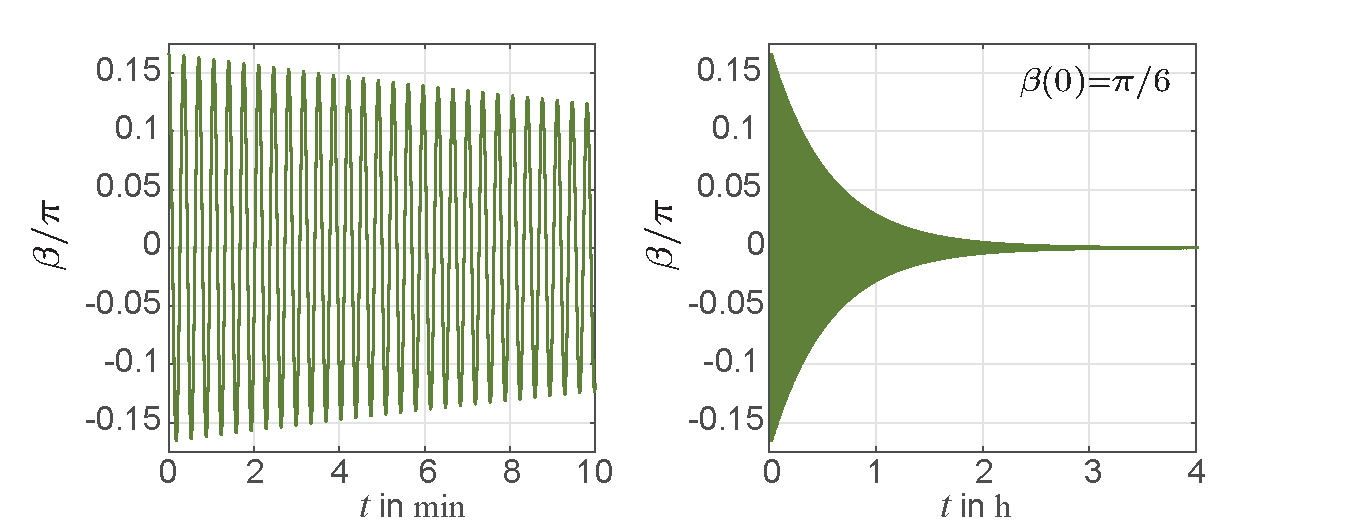
\includegraphics[width=\textwidth]{KreiselKomp1.pdf}%
    \caption[D�mpfung der Schwingung eines nordsuchenden Kreiselkompasses.]
    {D�mpfung der Schwingung eines nordsuchenden Kreiselkompasses um die
      Nord-S�d-Richtung. Die anf�ngliche Missweisung betr�gt $\beta(0)
      = \pi/6$. Parameter: $L_1 = \SI{-40}{\kg\metre\squared\per\second},\, J_{23}= \SI{0.02}{\kg\metre\squared},\,
			\vartheta = 90\degree - 50.9\degree,\, \gamma=\SI{0.001}{\per\second}$. Siehe \mscr~\mlbewref{KreiselKomp.m}.}
    \label{abb:bew_KreiselKompDaempfung1}
  \end{figure}

  Die anf�ngliche Missweisung spielt keine gro�e Rolle daf�r, wie lange die
  Schwingung ben�tigt, bis sie vollkommen ausged�mpft ist. Dies ist in
  \figref{bew_KreiselKompDaempfung2} zu erkennen, in der zwei
  weitere anf�ngliche Missweisungen, n�mlich $\pi/10 \, \hat{=} \, 18^\circ$
  und $2\pi/3 \, \hat{=} \, 120^\circ$ aufgetragen sind. Die Amplitude
  der Schwingung w�chst selbstverst�ndlich mit der anf�nglichen Missweisung,
  jedoch ist die prozentuale D�mpfung f�r alle Schwingungen �hnlich, wie es
  f�r einen linearen Reibungsterm zu erwarten ist. Auch f�r die sehr gro�e
  anf�ngliche Missweisung von $2\pi/3 \, \hat{=} \, 120^\circ$ findet der
  Kreiselkompass zuverl�ssig und einigerma�en z�gig die korrekte
  Nord-S�d-Richtung.

  \begin{figure}[H]\centering
    \centering
    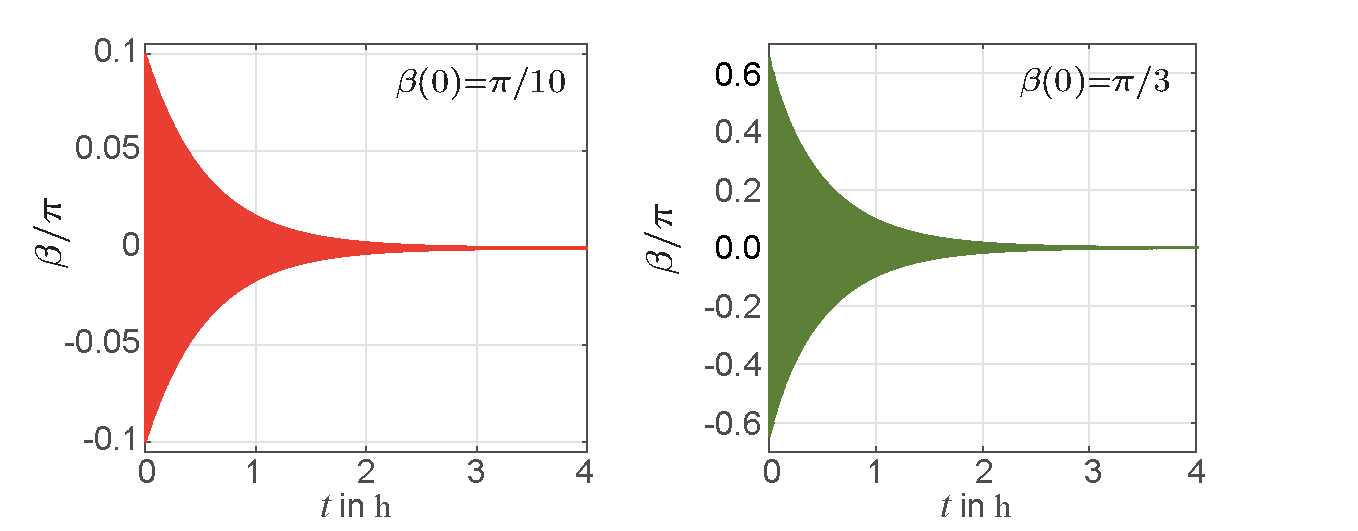
\includegraphics[width=\textwidth]{KreiselKomp2.pdf}%
    \caption[D�mpfung der Schwingung eines nordsuchenden Kreiselkompasses.]{
      D�mpfung der Schwingung eines nordsuchenden Kreiselkompasses um die
      Nord-S�d-Richtung f�r zwei weitere anf�ngliche Missweisungen der Betr�ge
      $\beta(0) = \pi/10$ und $\beta(0) = 2\pi/3$. Parameter: $L_1 = \SI{-40}{\kg\metre\squared\per\second},\, J_{23}= \SI{0.02}{\kg\metre\squared},\,
			\vartheta = 90\degree - 50.9\degree,\, \gamma=\SI{0.001}{\per\second}$. Siehe \mscr~\mlbewref{KreiselKomp.m}.}
    \label{abb:bew_KreiselKompDaempfung2}
  \end{figure}
  
Damit ein Kreiselkompass nach Norden zeigt, muss die Schwingung ged�mpft werden, damit sich das Ger�t auf dem Meridian niederlassen kann und ihn nicht st�ndig durchquert. Zur D�mpfung wurden zwei grunds�tzliche Methoden verwendet. Der erste, der in allen Kreiselkompassen au�er dem Sperry\footnote{Elmer Ambrose Sperry (1860--1930) war ein US-amerikanischer Erfinder und Gesch�ftsmann, der neben Hermann Ansch�tz-Kaempfe als einer der Entwickler der ersten verwendbaren Kreiselkompasse gilt. Sein Kreiselkompass wurde 1911 erstmals von der US-Marine eingesetzt.}\indexp{Sperry,Elmer Ambrose } verwendet wird, wurde von Schuler\footnote{Maximilian Schuler (1882--1972) war ein deutscher Ingenieur, Maschinenbauer und lehrte als Professor an der Hochschule in G�ttingen. Gemeinsam mit seinem Vetter Hermann Ansch�tz-Kaempfe war er der Erfinder des Mehrkreiselkompasses, der automatischen Schiffssteuerung und des Wendezeigers f�r Flugzeuge.}\indexp{Schuler, Maximilian} entwickelt. Dabei wird ein gegenpendelndes Drehmoment ausge�bt, das durch den eingeschr�nkten Fluss einer viskosen Fl�ssigkeit als Reaktion auf die Neigung des Kreiselelements verursacht wird. Viskosit�t und Str�mungsrichtung durch die Verengung werden so kombiniert, dass das Drehmoment phasenrichtig zur D�mpfung aufgebracht wird. Das Drehmoment ist horizontal und idealerweise so gerichtet, dass der Kreisel immer in Richtung des Meridians pr�zediert: Es zeigt nach Westen, wenn die Drehachse �stlich des Meridians liegt, und nach Osten, wenn die Drehachse westlich des Meridians liegt. Die kombinierte Wirkung von Pendel- und D�mpfungsdrehmomenten ver�ndert die zuvor erw�hnte elliptische Bewegung des unged�mpften Bereichs in eine spiralf�rmige Bewegung in Richtung des Meridians. Viskose Reibung absorbiert die entzogene Energie, um die D�mpfung zu bewirken.\\

Die zweite D�mpfungsmethode wird im Sperry-Kreiselkompass verwendet. Der Sperry-Kompass wird von einer Drahtaufh�ngung mit einem kraftbetriebenen Nachf�hrsystem, einem sogenannten Phantomring, getragen, einer Art Servomechanismus. Beim D�mpfen wird das Pendeldrehmoment so aufgebracht, dass durch die Interaktion mit dem Phantomring und dem Nachlaufmotor ein Drehmoment entlang der vertikalen Achse entsteht. Dadurch wird versucht, die Neigung des Kreiselelements zu verringern. Da Neigung und Bewegung in der horizontalen Ebene bei einem Kreiselkompass miteinander gekoppelt sind, dient diese Methode auch der D�mpfung der Rotationsachse zum Meridian hin. Die Energie zur D�mpfung liefert der Motor, der den Phantomring antreibt. Dieses System hat eine Antipendelwirkung und die D�mpfung wird durch die Zufuhr von Energie zum System erreicht.\\

Die Schwingungsdauer eines Kreiselkompasses wird durch die Anforderung bestimmt, dass der Kompass in einem beschleunigten Fahrzeug einwandfrei funktioniert. Die Pendelbewegung, die die Nordrichtung bewirkt, reagiert sowohl auf Fahrzeugbeschleunigungen als auch auf die Schwerkraft. Die mit den Nord-S�d-Beschleunigungen verbundenen Drehmomente (Ost-West-Beschleunigungen spielen aufgrund der Systemkonfiguration keine Rolle) w�rden eine entsprechende Abweichung des Kreiselkompasses um Norden verursachen und das Instrument f�r die Navigation unbrauchbar machen. Wenn ein Fahrzeug nach Norden oder S�den f�hrt, erreicht es bei seiner Bewegung �ber die kugelf�rmige Erde au�erdem im Verh�ltnis zum Tr�gheitsraum eine Winkelgeschwindigkeit, die senkrecht zur t�glichen Rotation der Erde steht. Dies bedeutet, dass der scheinbare Meridian, relativ zu dem die Sterne von einem fahrenden Fahrzeug aus auf- und untergehen w�rden, um eine vertikale Achse vom wahren Meridian gedreht ist, und zwar nach Westen bei n�rdlicher Geschwindigkeit und nach Osten bei s�dlicher Bewegung. Der Tangens dieses Drehwinkels ist die Nord-S�d-Geschwindigkeit des Fahrzeugs geteilt durch das Produkt aus der Erdgeschwindigkeit (Geschwindigkeit eines Punkts auf dem �quator, die 1667 km pro Stunde oder 900 Knoten betr�gt) und dem Kosinus des Breitengrads. Bei Schiffsgeschwindigkeit betr�gt dieser Winkel im Allgemeinen weniger als $4\degree$. Ein wichtiger Beitrag Schulers war die Entdeckung, dass bei einer Schwingungsdauer von 2�der Quadratwurzel aus Erdradius/Gravitation die Pr�zessionsrichtung der Drehachse des Gyroskops aufgrund der Beschleunigung genau der �nderungsrate des Winkels zwischen dem scheinbaren und dem wahren Meridian eines fahrenden Fahrzeugs entspricht. Der Kreiselkompass zeigt dann immer den wahren Norden an, wenn seine Anzeigereferenz um den Winkel zwischen diesen beiden Meridianen versetzt ist. Der Winkel ist bei Schiffsgeschwindigkeit eine direkte Funktion der Nord-S�d-Geschwindigkeit und kann einfach in das System eingestellt werden. Die Notwendigkeit einer genauen Geschwindigkeitsmessung f�r diesen Versatz ist der Hauptgrund, warum ein Kreiselkompass f�r den Einsatz in Flugzeugen nicht praktikabel ist.

\end{sol} 
%\href{PhysikUncut_Part1.pdf#prb:bew_gedaempfterKreiselkompass}{\textcolor{blue} {$\rightarrow$ zur \probref{bew_gedaempfterKreiselkompass}.}}\\
\textcolor{blue} {$\rightarrow$ zur} \probref{bew_gedaempfterKreiselkompass}.\\
\noindent\rule[1ex]{\textwidth}{0.5pt}  \newpage

%-----------------------------------------------------------------------------------------------------------
\hypertarget{lsg:bew_KreiselkompassLaengenkreis}{}
\begin{sol}{prob:bew_KreiselkompassLaengenkreis}\label{lsg:bew_KreiselkompassLaengenkreis} %�bung58
\textbf{Kreiselkompass bei Bewegung auf einem L�ngenkreis} \\ \\
Die Bewegung entlang eines L�ngenkreises kann durch einen zeitabh�ngigen Winkel $\vartheta$ beschrieben werden (\figref{bew_KreiselkompKS}). Die �nderung des Winkels $\vartheta$ beschreibt man am g�nstigsten durch eine
Drehung um die $y''$-Achse im Koordinatensystem K$''$ nach \figref{bew_KreiselkompKS}. Zur Transformation in das k�rperfeste 
Koordinatensystem K$''''$ m�ssen noch die Drehungen um die Winkel $\beta$
und $\alpha$ erfolgen. Es ergibt sich somit
\begin{multline*}
  \omega_L'''' = \begin{pmatrix} 1 & 0 & 0 \\ 0 & \cos\alpha
      & \sin \alpha \\ 0 & -\sin \alpha & \cos\alpha \end{pmatrix}
    \begin{pmatrix} \cos\beta & \sin \beta & 0 \\ -\sin\beta &
      \cos\beta & 0 \\ 0 & 0 & 1 \end{pmatrix} \begin{pmatrix} 0 \\
      \Omega_L \\ 0 \end{pmatrix} \\
    = \begin{pmatrix} 1 & 0 & 0 \\ 0 & \cos\alpha
      & \sin \alpha \\ 0 & -\sin \alpha & \cos\alpha \end{pmatrix}
    \begin{pmatrix} \sin \beta \\ \cos\beta \\ 0 \end{pmatrix} \Omega_L
    = \begin{pmatrix} \sin \beta \\ \cos\alpha\, \cos\beta \\ -\sin\alpha\,
      \cos\beta \end{pmatrix} \Omega_L \; .
\end{multline*}

Diese Rotation, im Fachjargon \textit{Transportrate} genannt, muss zur Winkelgeschwindigkeit
\eqref{eq:bew_WinkelgeschKreiselkompass} des feststehenden Kreiselkompasses
hinzuaddiert werden, sodass man
\begin{multline*}
  \vec{\omega}'''' = \vec{\omega}_\alpha'''' + \vec{\omega}_\beta''''
  + \vec{\omega}_E'''' + \omega_L''''
  = \begin{pmatrix} {\omega_1}'''' \\ {\omega_2}''''\\ {\omega_3}''''
  \end{pmatrix} \\
  =\begin{pmatrix} \dot{\alpha} -\sin\vartheta \cos\beta\, \Omega_E
    +\sin \beta \, \Omega_L \\
    \sin\alpha \, \dot{\beta} + \left ( \sin\vartheta \sin\beta \cos\alpha
      + \cos\vartheta \sin\alpha \right ) \Omega_E + \cos\alpha\, \cos\beta
    \, \Omega_L \\
    \cos\alpha \, \dot{\beta} + \left ( -\sin\vartheta \sin\beta \sin\alpha
      + \cos\vartheta \cos\alpha \right ) \Omega_E -\sin\alpha\, \cos\beta \,
    \Omega_L \end{pmatrix} \; .
\end{multline*}
erh�lt, was auf die modifizierte Lagrange-Funktion
\begin{multline*}
  \mathcal{L} = \frac{J_1}{2} \left ( \dot{\alpha} -\sin\vartheta \cos\beta \,
    \Omega_E +\sin \beta \, \omega_L \right )^2 
  + \frac{J_{23}}{2} \biggl \{ \dot{\beta}^2 + 2 \cos\vartheta \, \Omega_E \,
  \dot{\beta} \\
  + \left ( \sin^2\vartheta \sin^2\beta + \cos^2\vartheta
    \right ) \Omega_E^2 + 2 \sin\vartheta\, \sin\beta\, \cos\beta\Omega_E
    \Omega_L + \cos^2 \beta\, \Omega_L^2 \biggr \}
\end{multline*}
f�hrt. In dieser ist der Winkel $\alpha$ weiterhin eine zyklisch Koordinate, sodass wir die modifizierte
Erhaltungsgr��e
\begin{equation*}
  \frac{\partial \mathcal{L}}{\partial \dot{\alpha}} = J_1 \, \lk 
  \dot{\alpha} -\sin\vartheta \cos\beta \, \Omega_E + \sin \beta \, \Omega_L
  \rk = \tilde{L}_1'''' = \con
\end{equation*}
erhalten.
Weiterhin erhalten wir aus
\begin{equation*}
  \frac{\D}{\D t} \frac{\partial \mathcal{L}}{\partial \dot{\beta}}
  -\frac{\partial \mathcal{L}}{\partial \beta} = 0
\end{equation*}
die Bewegungsgleichung f�r $\beta$ als
\begin{multline*}
  J_{23} \ddot{\beta}  - J_{23} \sin\vartheta\, \Omega_E \, \Omega_L - L_1''''
  \left ( \sin\vartheta\, \sin\beta\, \Omega_E + \cos\beta\, \Omega_L \right )
  -  J_{23} \sin^2\vartheta\, \sin\beta\, \cos\beta\, \Omega_E^2 \\
  - J_{23} \sin\vartheta \left ( \cos^2\beta - \sin^2 \beta \right ) \Omega_E
  \Omega_L + J_{23} \cos\beta \sin\beta\, \Omega_L^2 = 0 \; .
\end{multline*}
Station�re L�sungen erhalten wir f�r $\ddot{\beta} = 0$, was auf eine Bestimmungsgleichung f�r $\beta$ f�hrt:
\begin{multline}
  - J_{23} \sin\vartheta\, \Omega_E \, \Omega_L - L_1''''
  \underbrace{\left ( \sin\vartheta\, \sin\beta\, \Omega_E + \cos\beta\, \Omega_L \right )}_{C_1}
  -  J_{23} \sin^2\vartheta\, \sin\beta\, \cos\beta\, \Omega_E^2 \\
  - J_{23} \sin\vartheta \left ( \cos^2\beta - \sin^2 \beta \right ) \Omega_E
  \Omega_L + J_{23} \cos\beta \sin\beta \Omega_L^2 = 0 \,.
  \label{eq:bew_KreiselKomp_Missweisung_exakt}
\end{multline}
Diese Gleichung muss numerisch nach $\beta$ gel�st werden.
Durch die schnelle Rotation $\dot{\alpha}$ des Kreisels dominiert jedoch der 
Term $C_1$. Die Erhaltungsgr��e $L_1$ ist wesentlich gr��er als alle anderen Terme
in der Gleichung. Daher gilt in guter N�herung, dass $\ddot{\beta} = 0$ wird, wenn
\begin{equation}
  C_1 = \sin\vartheta\, \sin\beta\, \Omega_E + \cos\beta\, \Omega_L = 0
  \label{eq:bew_KreiselKomp_Missweisung_Naeherung}
 \end{equation}
 \bzw
 \begin{equation*}
   \tan\beta = - \frac{\Omega_L}{\Omega_E}\frac{1}{\sin\vartheta}  
 \end{equation*}
gilt. Daran erkennt man sofort, dass die Missweisung  vom Breitengrad (repr�sentiert
 durch~$\vartheta$) abh�ngt, aber auch das Verh�ltnis der
 Bewegungsgeschwindigkeit~$\Omega_L$ zur Erdrotation~$\Omega_E$ entscheidend
 ist.  Um uns konkrete Beispiele vorzunehmen, nehmen wir an, dass die Bewegung auf
 dem Erdradius $R$ stattfindet, wie es f�r Schiffe typisch ist. Eine Fahrt
 mit der Geschwindigkeit~$v$ hat dann die Winkelfrequenz
 \begin{equation*}
   \Omega_L = \frac{v}{R}
 \end{equation*}
 zur Folge.
 Zahlenwerte, die mit \mscr~\mlbewref{KreiselKompMissweisung.m} berechnet wurden,
 kann man \figref{bew_KreiselKompMissweisung} entnehmen.
 \begin{figure}[H]\centering
   \centering
   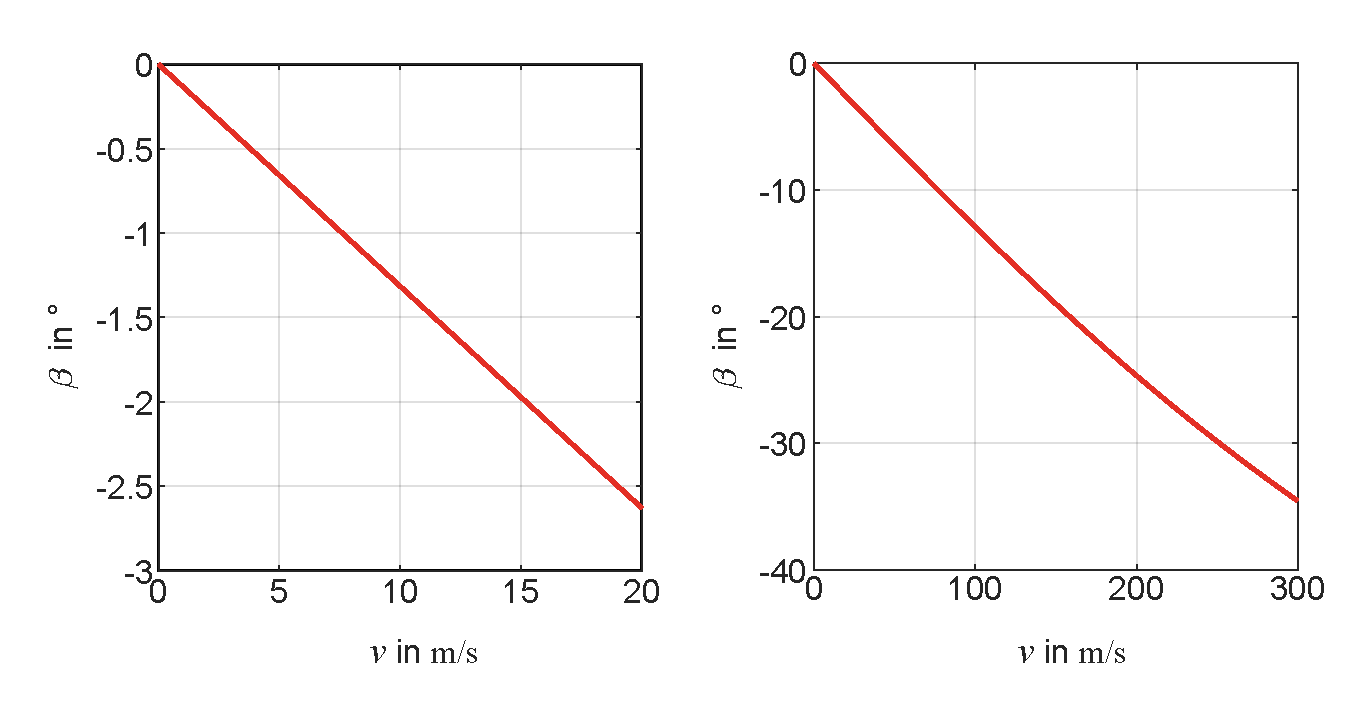
\includegraphics[width=\textwidth]{KreiselKompMissweisung.pdf}%
   \caption[Missweisung eines Kreiselkompasses]
   {Missweisung eines Kreiselkompasses bei einer Bewegung entlang eines
     L�ngengrads mit der Geschwindigkeit $v$. F�r Geschwindigkeiten, die
     Schiffe erreichen, bleibt sie moderat bei wenigen Grad. Jedoch tritt
     f�r die Geschwindigkeiten von Flugzeugen eine beachtliche Abweichung
     auf. Die Berechnung erfolgt nach Gleichung
     \eqref{eq:bew_KreiselKomp_Missweisung_exakt}. Parameter siehe \mscr~\mlbewref{KreiselKompMissweisung.m}.}
    \label{abb:bew_KreiselKompMissweisung}
  \end{figure}
  Dieses Beispiel ist f�r $20^\circ$ n�rdlicher Breite angegeben. Man erkennt
  deutlich, dass f�r typische Bewegungsgeschwindigkeiten von Schiffen
  $v < \SI{20}{\metre\per\second}$ die Abweichung mit Werten $\beta < 3^\circ$
  moderat bleibt. F�r Geschwindigkeiten, die Flugzeuge erreichen, sind jedoch
  erhebliche Abweichungen erkennbar.

\end{sol} 
%\href{PhysikUncut_Part1.pdf#prb:bew_KreiselkompassLaengenkreis}{\textcolor{blue} {$\rightarrow$ zur \probref{bew_KreiselkompassLaengenkreis}.}}\\
\textcolor{blue} {$\rightarrow$ zur} \probref{bew_KreiselkompassLaengenkreis}.\\
\noindent\rule[1ex]{\textwidth}{0.5pt}  \newpage


%-----------------------------------------------------------------------------------------------------------
\hypertarget{lsg:bew_DrehmomentPraezErde}{}
\begin{sol}{prob:bew_DrehmomentPraezErde}\label{lsg:bew_DrehmomentPraezErde} %�bung59
\textbf{Erdpr�zession} \\ \\
Wir berechnen zun�chst das Drehmoment von Sonne und Mond auf das Erdellipsoid. Wir schreiben in dieser L�sung der besseren Lesbarkeit wegen f�r $\vec{e}_\text{1} = \veceX\,,\, \vec{e}_\text{2} = \veceY\,,\, \vec{e}_\text{1}{}' = \vecpeX$ \usw und benutzen \figref{bew_DrehmomentPraezErde01}.

\begin{figure}[H]\centering
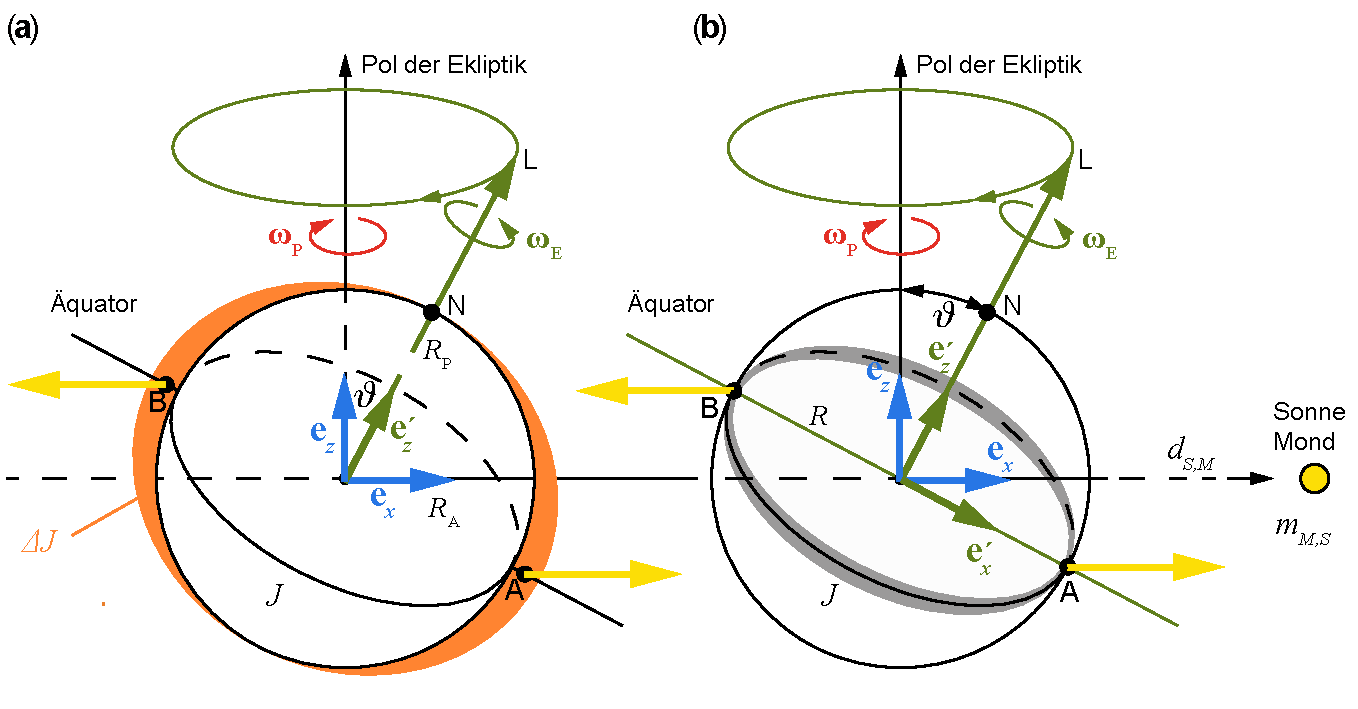
\includegraphics[width=1.0\textwidth]{ErdPraezession03.pdf}
\caption[Zur Geometrie der Erdpr�zession.]{\fa Geometrie der Erdpr�zession und \fb Modell der Erde als Kugel plus �quatorwulst (Ring um den �quator).} 
\label{abb:bew_DrehmomentPraezErde01}
\end{figure}

\begin{enumerate}
    \item 
    Das differentielle Drehmoment $\D \vec{M}_{\text{D},i}$, hervorgerufen von Sonne (S) und Mond (M) (angenommen als Massepunkte der Masse $m_i = m_\text{S},m_\text{M}$) an der Position $d_i\, \veceY$ auf das Massenelement $\D m = \varrho \D V'$ ist 
            \begin{align*}
                \D \vec{M}_{\text{D},i}\lk \vec{r}\rk = \vec{r}'\times\frac{G\,m_i\,\varrho\lk \vec{r}'\rk}{|\vec{r}-\vec{r}'|^3}\,\lk \vec{r}-\vec{r}'\rk \,\D^3V'\,.
            \end{align*}
    Hierin ist $\vec{r}$ der Ortsvektor $\vec{r} = d\,\veceY$ und $\varrho\lk \vec{r}'\rk$ die Dichte des Erdk�rpers. Wir haben hierbei \eqref{eq:bew_Drehmoment_starrer_K} benutzt. Der Nenner im Integranden beschreibt den Abstand des differentiellen Erdmassenelements $\D m$ zum Himmelsk�rper Mond \bzw Sonne.
    Wegen $\vec{r}' \times \vec{r}' = 0$ folgt f�r das gesamte Drehmoment durch Integration �ber das Volumen des Rotationsellipsoids 
            \begin{align}
                \vec{M}_{\text{D},i}\lk \vec{r}\rk = \int \vec{r}'\times\frac{G\,m_i\,\varrho\lk \vec{r}'\rk}{|\vec{r}-\vec{r}'|^3}\,\vec{r} \,\D^3\,V'\,. \label{eq:bew_DrehmomentPraezErde01}
            \end{align}
    \item
    Wir k�nnen den Nenner entwickeln, da die Ausdehnung der Erde viel kleiner ist als der Abstand zu den Himmelsk�rpern, d.\,h. $R_\text{E}, R_\text{A} \ll d$. Dazu schreiben wir:
            \begin{align*}
                \veceY &= \cos\vartheta\,\vecpeY + \sin\vartheta\,\vecpeZ \,, \\
                \vec{r}\,\, &= d\, \veceY \,, \\
                \vec{r}' &= r'\,\vec{e}_r' = r'\,\lk \cos\varphi'\,\vecpeX + \sin\varphi'\,\vecpeY\rk \,.
            \end{align*}
    Ferner ist 
            \begin{align*}
                \vec{r}\,\vec{r}' &= d_i\,r'\,\lk \cos\vartheta\,\vecpeY + \sin\vartheta\, \vecpeZ \rk \times \lk \cos\varphi'\,\vecpeX + \sin\varphi'\,\vecpeY\rk = d_i\,r'\,\cos\vartheta\,\sin\varphi'
            \end{align*}
    und 
            \begin{align*}
                |\vec{r}-\vec{r}'|^{-3} &= \lk \vec{r}^2 -2\vec{r}\,\vec{r}'+{\vec{r}'}^2 \rk ^{-\frac{3}{2}} = \lk {d_i}^2-2d_i\,r'\,\cos\vartheta\,\sin\varphi' + {r'}^2\rk ^{-\frac{3}{2}}  \\
                &= {d_i}^{-2}\,\underbrace{\lek 1- \underbrace{2\,\frac{r'}{d_i}\,\cos\vartheta\,\sin\varphi'}_{= x \ll 1} + \underbrace{\killA{\lk \frac{r'}{d_i}\rk^2}}_{\approx 0} \rek^{-\frac{3}{2}}}_{\lk 1-x\rk^{-\frac{3}{2}} \approx 1+\frac{3}{2}\,x} \\
                &\approx  {d_i}^{-2}\,\lk 1+3\frac{r'}{d_i}\,\cos\vartheta\,\sin\varphi'\rk \,.
            \end{align*}
    \item
    Wir betrachten nun den Ring mit seiner Massendichte in \figref{bew_DrehmomentPraezErde01}
            \begin{align*}
                \varrho \lk \vec{r}' \rk = \frac{m_\text{R}}{2\pi\,R_\text{E}}\,\delta\lk r'-R_\text{E}\rk\,\delta\lk z'\rk \,,
            \end{align*}
    worin $m_\text{R}$ die Gesamtmasse des Rings ist.
    \item
		F�r \eqref{eq:bew_DrehmomentPraezErde01} ergibt sich dann:
    \begin{align}
		\begin{split}
            \vec{M}_{\text{D},i}  = &\frac{G\,m_i\,m_\text{R}}{2\pi\,{d_i}^2\,R_\text{E}} \bigintsss \Biggl[ r'\lk \cos\varphi'\,\vecpeX + \sin\varphi'\,\vecpeY\rk \,\times \\  \label{eq:bew_DrehmomentPraezErde02}
						&\lek \delta (r'-R_\text{E})\,\delta (z') \, \lk 1+3\cos\vartheta\sin\varphi'\,\frac{r'}{d_i} \rk \rek \,\veceY \Biggl] \,r'\,\D r'\,\D y'\,\D z' \,,
		\end{split}
    \end{align}
		wobei wir hier das Volumenintegral wegen der Zylindersymmetrie des Erdk�rpers in Zylinderkoordinaten ausgef�hrt haben ($\D V' = r'\,\D r'\,\D y'\,\D z'$).
            \begin{align}
                \vec{M}_{\text{D},i} = &\frac{G\,m_i\,m_\text{R}\,R_\text{E}}{2\pi\,{d_i}^{2}}\,\bigintsss\limits_0^{2\pi} \Biggl[ \underbrace{\cos\varphi'}_{\int \ldots \D\varphi'= 0}\,\vecpeX\times \veceY+ \underbrace{\sin\varphi'}_{\int \ldots \D\varphi'= 0} \,\vecpeY\times \veceY\nonumber \\
                &+3\cos\vartheta\, \underbrace{\sin\varphi'\,\cos\varphi'}_{\int \ldots \D\varphi'= 0}\,\frac{R_\text{E}}{d_i}\,\vecpeX\times \veceY + 3\cos\vartheta \underbrace{\sin^2\varphi'}_{\int \ldots \D\varphi'= \pi} \frac{R_\text{E}}{d_i}\,\vecpeY\times \veceY \Biggl] \,\D\varphi' \nonumber \\ 
                &= \frac{3G\,m_i}{2{d_i}^{3}} \underbrace{m_\text{R}\,{R_\text{E}}^2}_{\Delta J}\,\cos\vartheta\,\vecpeY\times \veceY = \frac{3G\,m_i}{2{d_i}^{3}} \cos\vartheta\,\Delta J\,\vecpeY\times \veceY\,. \label{eq:bew_DrehmomentPraezErde03} 
            \end{align}
    Wir haben hiermit die auf den Kreisel (Ring) wirkenden Drehmomente der Gravitation von Sonne und Mond berechnet. Wie man an der dritten Potenz von $d_i$ im Nenner erkennt, sind es die Gezeitenkr�fte, die auf den Ring wirken.\\
\end{enumerate}
Wir wollen nun \eqref{eq:bew_DrehmomentPraezErde03} auswerten.
\begin{enumerate}
    \item 
    Aus \figref{bew_DrehmomentPraezErde01} sieht man, dass die Vektoren $\vecpeY$, $\veceY$ nur die f�r einen Zeitpunkt g�ltigen Achsen bzw. Richtungen darstellen, da sich die KOS $\sum'$ und $\sum'$ durch die Rotation der Erde und ihres Umlaufs um die Sonne gegeneinander \glqq verdrehen\grqq{}.\\
    Deswegen wandeln wir: 
            \begin{align*}
                \vecpeY\times \veceY &= \vecpeY \times \lk \cos\vartheta\,\vecpeY + \sin\vartheta\,\vecpeZ\rk = \sin\vartheta \lk \vecpeY\times \vecpeZ\rk = \sin\vartheta\, \vecpeX \,.
            \end{align*}
    Auch $ \vecpeX$ ist zeitlich ver�nderlich. Andererseits k�nnen wir schreiben
            \begin{align*}
                 \vecpeZ\times  \veceZ =  \vecpeZ \times \lk \cos\vartheta\, \vecpeZ - \sin\vartheta\, \vecpeY\rk = -\sin\vartheta\, \vecpeX 
            \end{align*} und erhalten:
            \begin{align*}
                 \vecpeZ\times \veceZ &= -\sin\vartheta\, \vecpeX = - \vecpeY\times \veceY \,.
            \end{align*}
    \item
    Da $ \vecpeZ$ und $ \veceZ$ �ber die Zeit konstant ist, haben wir nun eine von der Zeit unabh�ngige Darstellung f�r das Drehmoment gefunden:\footnote{Diese Herleitung gilt auch f�r andere Massenverteilungen, solange diese rotationssymmetrisch sind, \dh f�r $\varrho\lk \vec{r}{}'\rk$ h�ngt nicht von $\varphi'$ ab, d.h. $\int \varrho\lk \vec{r}{}'\rk \,\sin\varphi'\,\cos\varphi'\,\D V' = 0$.}
            \begin{align}
                \vec{M}_{\text{D},i} = \frac{3G\,m_i}{2{d_i}^{3}}\,\cos\vartheta\,\Delta J\, \vecpeZ \times \veceZ\,. \label{eq:bew_DrehmomentPraezErde04}
            \end{align}
    \item
    Wir k�nnen jetzt noch die Pr�zessionsfrequenz bestimmen. Dazu schreiben wir \eqref{eq:bew_DrehimpulsSatz} f�r den hier vorliegenden Fall als:
            \begin{align*}
                \frac{\D \vec{L}}{\D t} &= \sum_i \vec{M}_{\text{D},i} = \vec{M}_\text{D, ges} = \frac{\D ( L \,\vecpeZ)}{\D t} = L\,\frac{\D \vecpeZ}{\D t} = L\,\vec{\omega}_\text{P}\times \vecpeZ \,,
            \end{align*}
Im letzten Schritt haben wir \eqref{eq:bew_Rot_System2} benutzt. F�r die Richtungs�nderung (Pr�zession) des Drehimpulses folgt dann:							
            \begin{align*}
                L\,\vec{\omega}_\text{P}\times \vecpeZ &= \vec{M}_\text{D, ges} = |\vec{M}_\text{D, ges}|\,\vecpeZ\times \veceZ = -|\vec{M}_\text{D, ges}|\,\veceZ\times \vecpeZ\,, 
						\end{align*}
						und damit
            \begin{align}
                 L\,\vec{\omega}_\text{P} &= -|\vec{M}_\text{D, ges}|\,\veceZ ~~\rightarrow~~\vec{\omega}_\text{P} = -\frac{|\vec{M}_\text{D, ges}|}{L}\,\veceZ~~\rightarrow~~ |\vec{\omega}_\text{P}| = -\frac{|\vec{M}_\text{D, ges}|}{J_\text{z}\,\omega_\text{E}} \,. \label{eq:bew_DrehmomentPraezErde05}
            \end{align}
Die Erdachse pr�zediert also um $\veceZ$ und entgegengesetzt zum Umlauf der Erde um die Sonne, der Betrag der Pr�zessionsfrequenz ist durch $|M|/(J_\text{z}\,\omega_\text{E})$ gegeben.
Es ist etwas erstaunlich, dass unsere N�herung, dass Mondbahnebene und Ekliptik zusammenfallen (obwohl zwischen beiden eine mittlere Neigung von etwa $5\degree$ besteht), doch eine recht gute �bereinstimmung mit den experimentellen Befunden gibt.
Das kann erkl�rt werden, dass die Pr�zession auf Grund der relativ geringen Abplattung sehr viel langsamer ist als die Mondbewegung und damit eine in der Ekliptik liegende Mondmasse eine gute N�herung darstellt.
\end{enumerate}

Im Kapitel Himmelsmechanik (Band II) werden wir entsprechende Drehmoment der Pr�zession f�r ein Rotationsellipsoid �ber eine Entwicklung seines Gravitationspotentials nach Kugelfl�chenfunktionen berechnen. Die dort dargestellte Methode verk�rpert den allgemeinen Weg, wie man f�r eine beliebige Form- bzw. Massenverteilung $\varrho(\vec{r})$ das gravitative Potential \bzw Drehmoment berechnen kann. \\

\end{sol} 
%\href{PhysikUncut_Part1.pdf#prb:bew_DrehmomentPraezErde}{\textcolor{blue} {$\rightarrow$ zur \probref{bew_DrehmomentPraezErde}.}}\\
\textcolor{blue} {$\rightarrow$ zur} \probref{bew_DrehmomentPraezErde}.\\
\noindent\rule[1ex]{\textwidth}{0.5pt}  \newpage


%%%-----------------------------------------------------------------------------------------------------------
%%%-----------------------------------------------------------------------------------------------------------
\newpage

\subsection{�bungen zu den Lagrange-Gleichungen f�r komplexe System}

\medskip

%-----------------------------------------------------------------------------------------------------------
\hypertarget{lsg:bew_laundromat}{}
\begin{sol}{prob:bew_laundromat}\label{lsg:bew_laundromat} %�bung60
\textbf{Physik in der Waschmaschine}  \\ \\
Das Anlauf- und Auslaufverhalten einer Trommelwaschmaschine ist eine sch�ne Anwendung der Lagrange-Methode f�r einen festen K�rper. Interessanterweise f�hrt die Methode f�r eine mit Federn aufgeh�ngte Trommel der Masse $m$ und des Radius $R$, die mit einer exzentrischen Masse $m_\text{E}$ beladen ist, auf Bewegungsgleichungen, die denen f�r ein Doppelpendel �hneln \cite{Denny2010}. \\
Wir wollen ein vereinfachtes Modell nach \figref{bew_laundromat01} annehmen, nach der die symmetrische Trommel ein sogenannter Frontloader ist, der an vier Federn aufgeh�ngt ist. Die Unsymmetrie durch die Masse $m_\text{E}$ sei auf dem Rand der Trommel fest lokalisiert.\footnote{In der Realit�t wird diese Masse durch Einfluss der Schwer- und Fliehkraft sich bei der Rotation der Trommel relativ zum Trommelzentrum bewegen.} \\
Wir sind an den Vibrationen der Trommel interessiert und wollen diese mit den Koordinaten des Trommelzentrums beschreiben ($x=x_\text{M}$, $z=z_\text{M}$). \\
Die Position der Masse $m_\text{E}$ sei durch $x_\text{E}$, $z_\text{E}$ gegeben. Nach \figref{bew_laundromat01} gilt:\footnote{Man beachte, dass $\varphi$ anders als sonst �blich definiert ist.}
\begin{align}
\begin{split}
    x_\text{E} &= x + R\,\sin\varphi\,, \\
    z_\text{E} &= z-R\,\cos\varphi\,.
\end{split} \label{eq:bew_laundromat01}
\end{align}
Die kinetische und die potentielle Energie sind gegeben:
\begin{subequations}
\begin{align}
    T &= \frac{1}{2}\,m\lk \dot{x}^2 + \dot{z}^2\rk + \frac{1}{2}J\,\dot{\varphi}^2 + \frac{1}{2}m_\text{E}\,v_\text{E}{}^2\,, \label{eq:bew_laundromat02a} \\
    U &= m_\text{E}\,g\,z_\text{E} + m\,g\,z + \frac{1}{2}K\lk x^2+z^2\rk\,, \label{eq:bew_laundromat02b}
\end{align}
\end{subequations}
worin $J\approx m\,R^2$ das Tr�gheitsmoment der Trommel ist und $v_\text{E}$ die Geschwindigkeit der Masse $m_\text{E}$ im KOS $\vec{\Sigma}$:
\begin{align*}
    v_\text{E}{}^2 = \lk \dot{x}_\text{E}{}^2 + \dot{z}_\text{E}{}^2\rk = \lk \dot{x} + R\,\dot{\varphi}\,\cos\varphi\rk^2 + \lk \dot{z} + R\,\dot{\varphi}\,\sin\varphi\rk^2\,.
\end{align*}
Unter Hinzuf�gen eines Reibungsterms $\frac{1}{2}\Gamma\lk \dot{x}^2 + \dot{z}^2\rk$ erhalten wir aus der Lagrange-Funktion die Bewegungsgleichungen f�r $x$ und $z$:
\begin{align}
\begin{split}
    \ddot{x} + \eta\,\dot{x} + \omega_0{}^2\,x &= -B\,\frac{\D}{\D t}\lk \dot{\varphi}\,\cos\varphi\rk\,, \\
    \ddot{z} + \eta\,\dot{z} + \omega_0{}^2\,z + g &= -B\,\frac{\D}{\D t}\lk \dot{\varphi}\,\sin\varphi\rk\,, \label{eq:bew_laundromat03}
\end{split} 
\end{align}
worin 
\begin{align*}
    \omega_0{}^2 = \frac{k}{m+m_\text{E}}\,, ~~~~ B=\frac{m_\text{E}}{m+m_\text{E}}\,R\,, ~~~~ \eta = \frac{\Gamma}{m+m_\text{E}}\,.
\end{align*}
Man findet sehr einfach, wie in Kap. \ref{kap:bew_pendulum} gezeigt, die station�re L�sung von \eqref{eq:bew_laundromat03} f�r eine mit $\Omega = \dot{\varphi} = \text{const}$ rotierende Trommel:
\begin{align}
\begin{split}
    x &= R_0\,\sin\lk \Omega \,t -\varphi_0\rk \,, \\
    z &= R_0\,\cos\lk \Omega \,t -\varphi_0\rk - \frac{g}{\omega_0{}^2}\,,
\end{split} \label{eq:bew_laundromat04}
\end{align}
mit 
\begin{align*}
    R_0 = \frac{B\,\Omega^2}{\sqrt{\lk \omega_0{}^2-\Omega^2\rk^2 + \eta^2\,\Omega}}\,, ~~~~ \tan\varphi_0 = \frac{\eta\,\Omega}{\omega_0{}^2-\Omega^2}\,.
\end{align*}
Das sind die L�sungen des ged�mpften harmonischen Oszillators. \\
Wir sind aber an der Hochlaufphase (und an der Auslaufphase) der Trommelwaschmaschine interessiert und k�nnten dazu in \eqref{eq:bew_laundromat03} eine N�herung machen, in der $\dot{\varphi}$ f�r die Hochlaufphase ann�hernd als konstant angenommen wird.\footnote{Man kann davon ausgehen, das f�r diese Phase das auftreibende Drehmoment konstant ist.} Es ergibt sich dann f�r die Position des Trommelmittelpunktes mit 
\begin{align*}
    T = \frac{\Omega\,t^2}{2\varphi} ~~~~ \text{bzw.} ~~~~ \varphi\lk t\rk = \frac{\Omega}{T}\,\frac{t^2}{2}
\end{align*}
n�herungsweise
\begin{align}
    R_0\lk t \rk = B\,\frac{\lk \Omega \,t\rk^2}{\sqrt{\lek\lk \omega_0 \,T\rk^2 - \lk  \Omega t\rk^2\rek^2 + \lk \eta\,T\rk^2\lk\Omega \,t\rk^2}}\,.  \label{eq:bew_laundromat05} 
\end{align}
$T$ ist die Dauer der Hochlaufphase. \\
Man erkennt, dass es bei $t_\text{Res} = \omega_0\,T/\Omega$ zu der gr��ten Amplitude der Trommelvibration kommt mit einem Wert von
\begin{align*}
    R_\text{0,max} = \frac{B\,\omega_0}{\eta}\,.
\end{align*}
In \mlbewref{Waschmaschine01.m} l�sen wir das DGL-System \eqref{eq:bew_laundromat03} numerisch f�r einen typischen Parametersatz von:
\begin{align*}
    R = \SI{0.25}{\cm}\,, ~~~~m = \SI{10}{\kg}\,, ~~~~ \omega_0 = 2\pi\cdot\SI{4}{\Hz} \approx \SI{25}{\radian\per\second}\,, ~~~~ T \approx \SI{25}{\second}\,, \\
    \frac{m_\text{E}}{m} \approx \SI{0.1}{}\ldots \SI{0.2}{}\,, ~~~~ \eta = 2\cdot\omega_0\,, ~~~~ \Omega = 2\pi\cdot\SI{20}{\Hz} \approx \SI{125}{\radian\per\second}\,.
\end{align*}
Die Ergebnisse sind in \figref{bew_laundromat02} und \figref{bew_laundromat03} f�r die Hochlauf- bzw. Auslaufphase zu sehen. 
\begin{figure}
  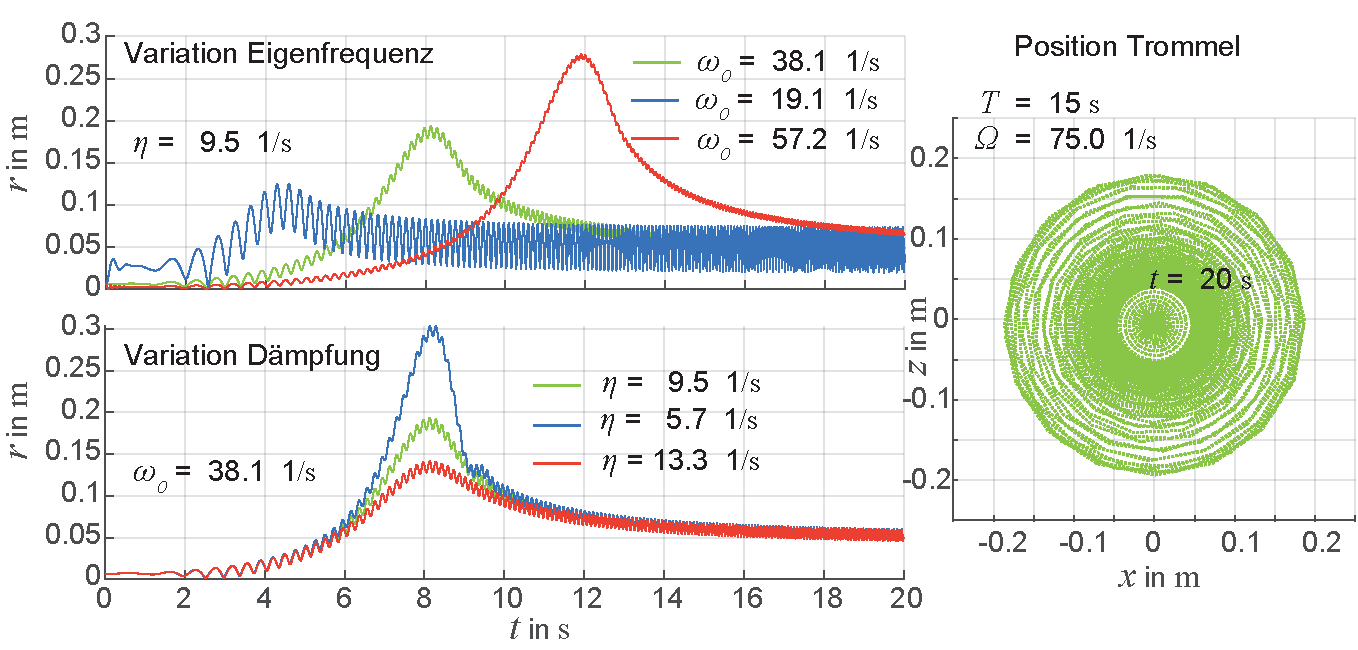
\includegraphics[width=\textwidth]{Waschmaschine01.pdf}
  \caption[Anlaufverhalten einer Trommelwaschmaschine]{Anlaufverhalten einer Trommelwaschmaschine} \label{abb:bew_laundromat02}
\end{figure}
\begin{figure}
  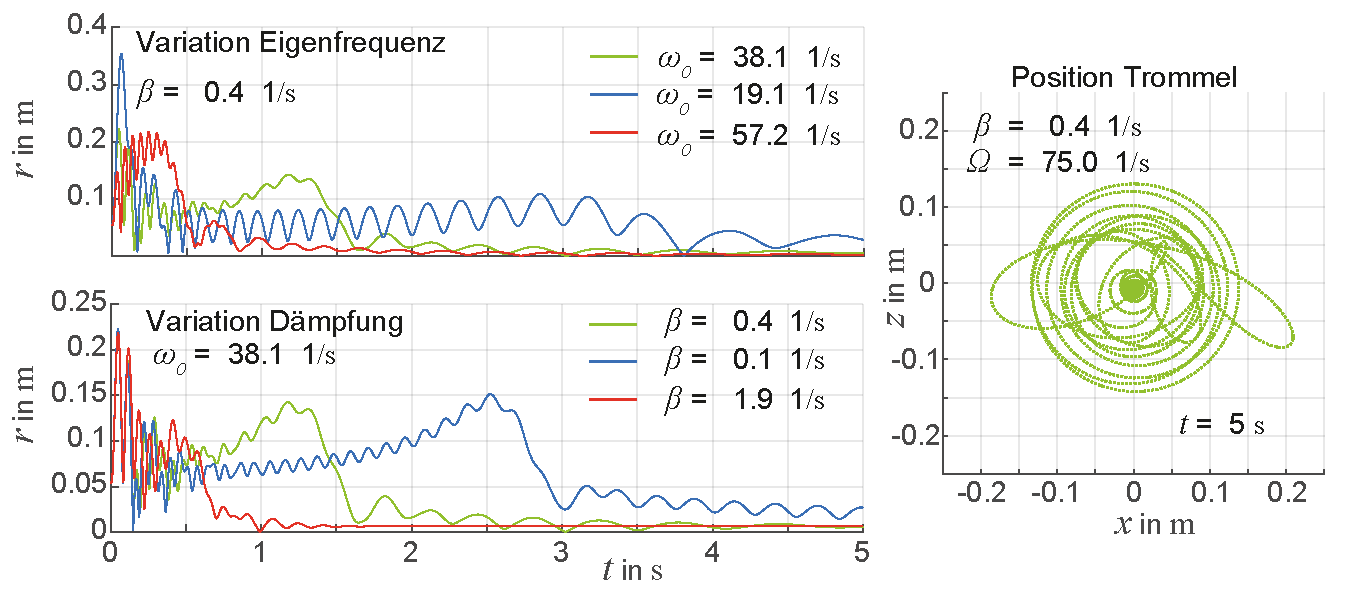
\includegraphics[width=\textwidth]{Waschmaschine02.pdf}
  \caption[Auslaufverhalten einer Trommelwaschmaschine]{Auslaufverhalten einer Trommelwaschmaschine} \label{abb:bew_laundromat03}
\end{figure}
Man erkennt beim Hochlaufen das Durchlaufen einer Resonanz und das Einschwingen auf die station�re Vibration der Trommel. \\
Beim Auslaufen (\mlbewref{Waschmaschine02.m}) benutzen wir f�r den Winkel $\varphi$ die folgende Lagrange-Gleichung, die ebenfalls aus der Lagrange-Funktion $\mathcal{L}$ �ber \eqref{eq:bew_laundromat02a} und \eqref{eq:bew_laundromat02b} gewonnen werden kann. Wir f�hren einen weiteren Reibungsterm $\beta$ ein, der die Reibung der Trommel bei abgeschaltetem Motor beschreibt und erhalten die DGL f�r $\varphi(t)$: 
\begin{align}
    \ddot{\varphi} + \beta\,\dot{\varphi} = Q\,\lk x\,\cos\varphi + z\,\sin\varphi\rk + P\,\lk \dot{x}\,\cos\varphi + \dot{z}\,\sin\varphi\rk \label{eq:bew_laundromat06}
\end{align}
mit
\begin{align*}
    Q &= \frac{m_\text{E}}{m\,R}\,\frac{m+m_\text{E}}{m+2m_\text{E}}\,\omega_0{}^2\,,\\
    P &= \frac{m_\text{E}}{m\,R}\,\frac{m+m_\text{E}}{m+2m_\text{E}}\,\eta \,.
\end{align*}
Zusammen mit den DGL f�r $x(t)$ und $z(t)$ nach \eqref{eq:bew_laundromat03} haben wir ein numerisch l�sbares System f�r die Auslaufphase. Diese unterscheidet sich von der Hochlaufphase darin, dass die Variable $\varphi$ wie $x$, $z$ ebenfalls eine freie Variable ist. 

\end{sol} 
%\href{PhysikUncut_Part1.pdf#prb:bew_laundromat}{\textcolor{blue} {$\rightarrow$ zur \probref{bew_laundromat}.}}\\
\textcolor{blue} {$\rightarrow$ zur} \probref{bew_laundromat}.\\
\noindent\rule[1ex]{\textwidth}{0.5pt}  

%-----------------------------------------------------------------------------------------------------------
\newpage
\hypertarget{lsg:bew_achterbahn}{}
\begin{sol}{prob:bew_achterbahn}\label{lsg:bew_achterbahn} %�bung61
\textbf{Physik auf der Achterbahn I} \\ \\

\begin{figure}
  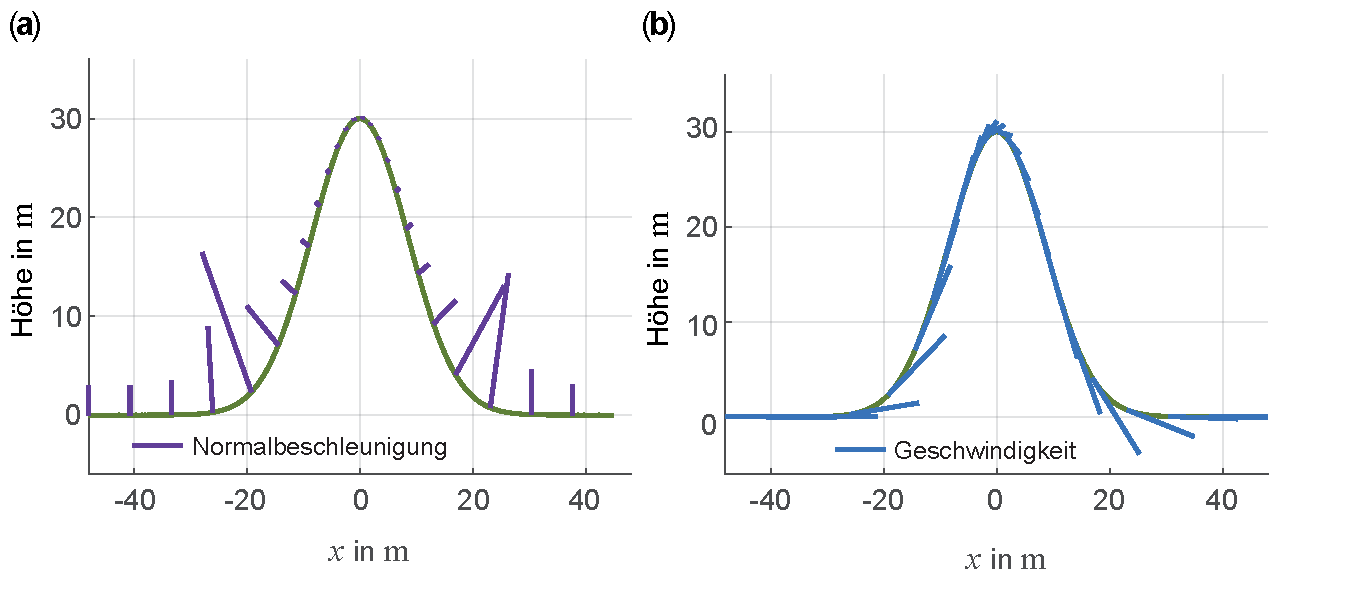
\includegraphics[width=\textwidth]{Achterbahn02.pdf}
  \caption[Gau�-Kurve als Beispiel f�r eine Achterbahn-Ausschnitt.]{Gau�-Kurve als Beispiel f�r eine Achterbahn-Ausschnitt.} \label{abb:bew_Achterbahn02}
\end{figure}

Wir wollen zun�chst wieder einen einzelnen Wagen auf einem beliebigen Abschnitt der Achterbahn betrachten und anschlie�end einen ganzen Zug. Wir wollen uns dabei auf die grunds�tzliche physikalischen Methoden fokussieren und bewusst einige eher allgemeing�ltige Vorgehensweisen w�hlen, obwohl es durchaus einfachere L�sungen, \zb auf Basis der Newtonschen Mechanik denkbar w�ren. \\

\begin{enumerate}
    \item [1)] \textit{\textbf{Bewegungsgleichung und Kr�fte eines Massepunktes auf einer beliebigen Kurve}} \\
		
    Die Achterbahn sei durch eine Kurve $z=h\lk x\rk$ gegeben. Diese stellt im Prinzip die Zwangsbedingung f�r die Bewegung dar, denn der Massepunkt soll sich ja genau auf dieser Kurve bewegen, wozu bestimmte Zwangskr�fte erforderlich sind:
    \begin{align}
        f = z-h\lk x\rk = 0 \,. \label{eq:bew_Achterbahn00}
    \end{align}
    Wir wollen die Methode der Lagrange-Multiplikatoren benutzen und brauchen wegen \eqref{eq:bew_Achterbahn00} einen Lagrange-Multiplikator $\lambda$. Wir bilden nach der Vorschrift in \kapitel{bew_Lagrange_I}:
    \begin{align}
        0 = \dot{f} &= \dot{z} - \frac{\d h}{\d x}\,\dot{x}\,, \nonumber \\
        0 = \ddot{f} &= \ddot{z} - \underbrace{\frac{\d^2 h}{\d x^2}\,\dot{x}^2 }_{\substack{g_f\lk x,\dot{x}\rk}}- \frac{\d h}{\d x}\,\ddot{x} = \ddot{z} - \frac{\d h}{\d x}\,\ddot{x} - g_f\lk x,\dot{x}\rk\,. \label{eq:bew_Achterbahn02}
    \end{align} 
    Die Bewegungsgleichung f�r den Massepunkt auf der Kurve lautet:
    \begin{align}
    \begin{split}
        m\,\ddot{x} &= \lambda \,\frac{\d f}{\d x} = -\lambda\,\frac{\d h}{\d x}\,, \\
        m\,\ddot{z} &= -m\,g + \lambda\,\frac{\d f}{\d z} = -m\,g + \lambda \,. 
    \end{split} \label{eq:bew_Achterbahn03} 
    \end{align} 
    Wir k�nnen nun \eqref{eq:bew_Achterbahn02} in \eqref{eq:bew_Achterbahn03} einsetzen, setzen $\frac{\lambda}{m} \rightarrow \lambda$ und erhalten:
    \begin{align}
        0 = -g + \lambda + \lambda\,\lk \frac{\d h}{\d x}\rk^2 - \frac{\d^2 h}{\d x^2}\,\dot{x}^2 \label{eq:bew_Achterbahn04} 
    \end{align}
    als Bestimmungsgleichung f�r $\lambda$, woraus wir f�r eine beliebige Kurvenform $h\lk x\rk$ die Zwangskraft (Zwangsbeschleunigung) $\lambda$ bestimmen k�nnen. 
    \begin{align}
        \lambda (x,  \dot{x}) = \frac{g + \frac{\d^2 h}{\d x^2}\,\dot{x}^2}{1+\lk \frac{\d h}{\d x}\rk ^2} \,. \label{eq:bew_Achterbahn05} 
    \end{align}

\noindent{\color{black} \rule{\textwidth}{0.2 mm}} \\

\textbf{\textit{Beispiel Gau�-Kurve}}
    \begin{align}
    \begin{split}
        h \lk x \rk &= H\,\e^{-a^2\,x^2} ~~ \text{mit} ~~ x_P = 0\,, ~~ a^2 = \frac{\ln 2}{B^2} \\
        \frac{\d h}{\d x} &= -2a^2\,x\,H\,\e^{-a^2\,x^2} \\
        \lk \frac{\d h}{\d x}\rk^2 &= 4a^4\,H^2\,x^2\,\e^{-2a^2\,x^2} \\
        \frac{\d^2 h}{\d x^2} &= \lk +4\,a^4\,x^2\,H - 2a^2\,H\rk \, \e^{-a^2\,x^2} = 2a^2\,H\lk 2a^2\,x^2-1\rk\,\e^{-a^2\,x^2} \,.
				\label{eq:bew_Achterbahn06} \\
    \end{split} 
		\end{align} 

\noindent{\color{black} \rule{\textwidth}{0.2 mm}} \\ 

Die Bewegungsgleichungen \eqref{eq:bew_Achterbahn03} k�nnen mit \eqref{eq:bew_Achterbahn05} numerisch integriert werden (\figref{bew_Achterbahn02}).
F�r die Beschleunigungen zur Verwendung in \mlbewref{Achterbahn01.m} schreiben wir \\
\begin{subequations}
\begin{align}
\ddot{x} &= -\frac{\lk h''\,\dot{x}^2+g\rk}{1+ \lk h'\rk^2}\, h' = a_x \label{eq:bew_Achterbahn10a}\,, \\
\ddot{z} &= \frac{-g\,\lk 1 + \lk h'\rk^2\rk + g + h''\,\dot{x}^2}{1 + \lk h'\rk^2} = \frac{-g\,\lk h'\rk^2 + h''\,\dot{x}^2}{1+ \lk h'\rk^2} = a_z \,, \label{eq:bew_Achterbahn10b} \\
a_z &= h''\,\dot{x}^2 + h'\,a_x\,. \label{eq:bew_Achterbahn10c}
\end{align}
\end{subequations}
Die Kr�fte, die auf den Massepunkt wirken, ergeben sich mit $m\,\ddot{x}$ \bzw $m\,\ddot{z}$ und die Summe von Zwangskraft (Normalkraft) und Gewichtskraft\footnote{Man kann leicht zeigen, dass f�r ein Teilchen auf einer Kreisbahn, diese Summe gleich der Radialkraft ist, $\vec{F}_\text{G} +\vec{F}_\text{N}$ k�nnte man daher auch als verallgemeinerte Zentripetalkraft bezeichnen.} ist dann:
\begin{align}
\begin{split}
    \vec{F}_\text{G} +\vec{F}_\text{N} &= 
    \begin{pmatrix}
    m\,a_x\\
    m\, a_z 
    \end{pmatrix}
    = 
    \frac{m}{1 + \lk h'\rk^2}
    \begin{pmatrix}
    -\lk h''\,\dot{x}^2 + g\rk\,h' \\
    h''\,\dot{x}^2 - g\,\lk h'\rk^2
    \end{pmatrix} \\
    &= \frac{m}{1 + \tan^2\theta}
    \begin{pmatrix}
    -\lk h''\,\dot{x}^2 + g\rk\,\tan\theta \\
    h''\,\dot{x}^2 - g\,\tan^2\theta 
    \end{pmatrix} \,. \label{eq:bew_Achterbahn11}
\end{split} 
\end{align} 
Wir haben dabei 
	\[h' = \frac{\d h}{\d x} = \frac{\d z}{\d x} = \tan\theta	
	\]
benutzt, worin $\theta$ der Winkel der Tangente an die Bahnkurve relativ zur $x$-Achse ist (\figref{bew_Achterbahn02}).
In \mlbewref{Achterbahn01.m} haben wir f�r die Gau�-Kurve die Geschwindigkeit, Beschleunigung und die Richtung Gesamtkraft berechnet und in \figref{bew_Achterbahn03} aufgetragen.
Die Anfangsbedingung bei $x_0 = -4/a$, $z_0 = h\lk x_0\rk$ haben wir so gew�hlt, dass der Massepunkt sicher die H�he $H$ erreicht, also
\begin{align*}
    \dot{x}(0) =\dot{x}_0 \geq \sqrt{\frac{2\,g\,H}{1 + h'\lk x_0\rk^2}}\, && \dot{z}(0)=\dot{z}_0 = h'\lk x_0\rk \,\dot{x}_0\,.
\end{align*}
Das Ergebnis der Rechnungen ist in \figref{bew_Achterbahn03} aufgetragen.
Als Parameter haben wir gew�hlt $H = \SI{30}{\metre}$, $B= \SI{10}{\metre}$, $a = \sqrt{\ln 2}/\SI{10}{\metre}$. \\
Man erkennt aus \figref{bew_Achterbahn03a} sehr sch�n, dass abh�ngig von der Position auf der Bahnkurve der Massepunkt Beschleunigungen gr��er als $g$ erfahren kann, aber auch kleiner als $g$. Die Phasen, in denen die Beschleunigung in Richtung $z$ kleiner als Null ist bezeichnet man als "`\textit{Airtime}"', da ein mitbewegter K�rper quasi schwerelos w�re oder sogar nach oben fliegen w�rde. Diese Airtime tritt vor allem am Hochpunkt der Gau�-Kurve auf und ist dabei um so st�rker, je st�rker die Kr�mmung der Kurve ist. Umgekehrt w�rde ein mitbewegter K�rper an den in \figref{bew_Achterbahn02} gekennzeichneten Stellen stark in die "`Sitze gedr�ckt"'.\\

\begin{figure}
  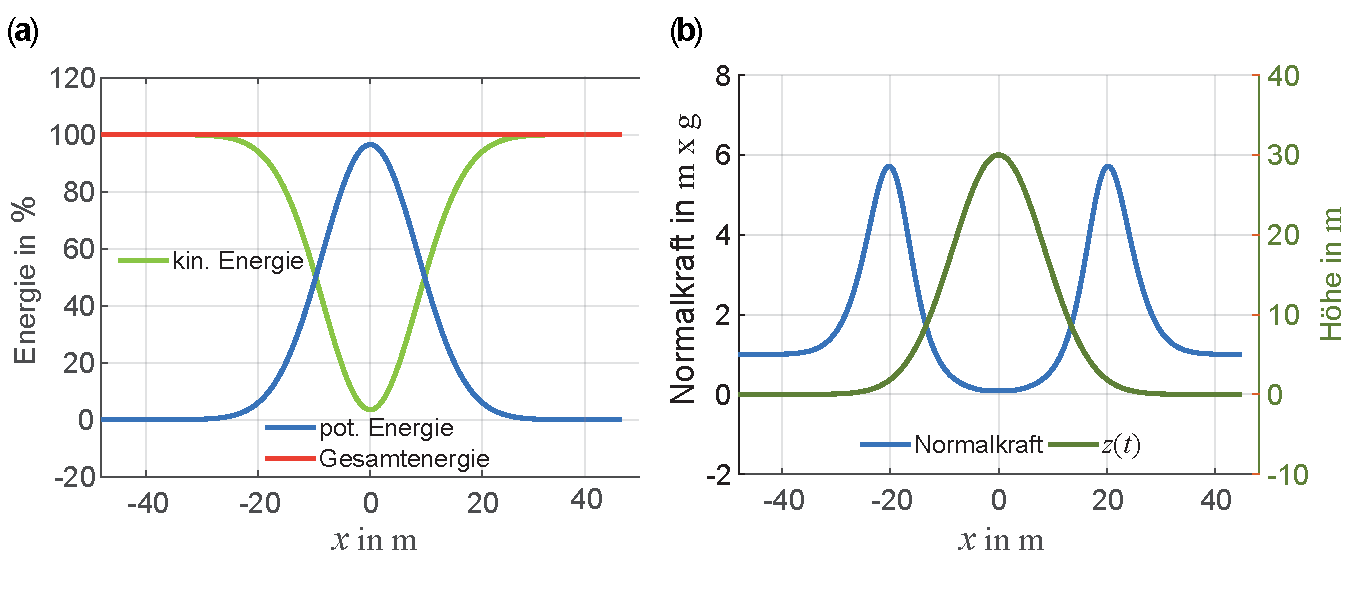
\includegraphics[width=\textwidth]{Achterbahn03a.pdf}
  \caption[Energieverteilung und Beschleunigung eines Massepunktes]{Energieverteilung \fa und Beschleunigung \fb eines Massepunktes auf einer Gau�-Kurve.} \label{abb:bew_Achterbahn03}
\end{figure}

\begin{figure}
  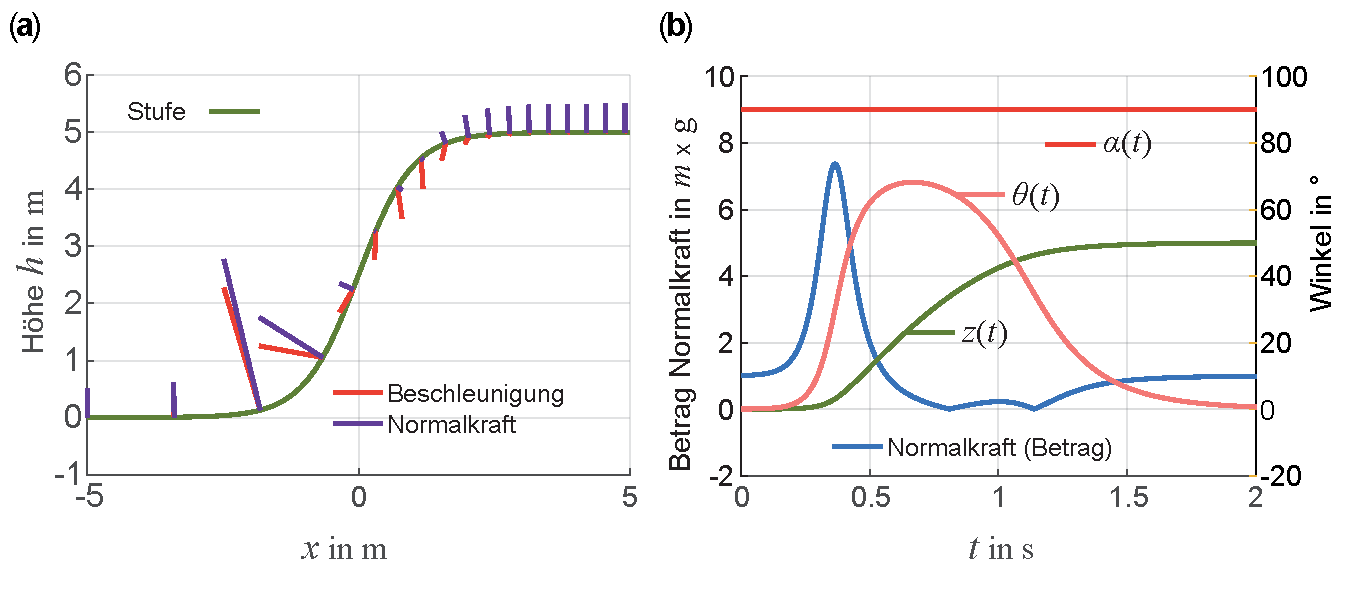
\includegraphics[width=\textwidth]{Achterbahn03b.pdf}
  \caption[Bewegung eines Massepunktes auf einer Stufenkurve]{\fa Beschleunigungsrichtung und \fb Normalkraft, Winkel der Geschwindigkeit eines Massepunktes auf einer Stufenkurve der Form $z(x) = 1 + \tanh(x)$} \label{abb:bew_Achterbahn03a}
\end{figure}
\newpage
    \item [2)] \textit{\textbf{Bewegungsgleichung und Kr�fte eines Massepunktes in einer Loop}} \\
		
Wir wollen nun einen Massepunkt in einer Loop betrachten (\figref{bew_Achterbahn02}) und auch berechnen, mit welcher Geschwindigkeit der Massepunkt mindestens in die Loop einfahren muss, damit er sie komplett durchlaufen kann. Dazu ist es notwendig, dass die Kurve in parametrisierter Form, also
\begin{align*}
  x = x\lk u\rk ~~~\text{und}~~~z = z\lk u\rk 
\end{align*}
vorliegt, da $z$ ja f�r ein und dasselbe $x$ mehrere Werte haben kann. Der Parameter $u$ muss keine physikalische Bedeutung haben und kann dimensionslos sein. Durch die Parametrisierung wird die Eindeutigkeit hergestellt, die wir \zb f�r die Berechnung des Durchfahrens einer Loop ben�tigen. Wir finden durch Differenzieren:
\begin{subequations}
\begin{align}
    v_x &= \frac{\d x}{\d u}\,\dot{u} = x'\,\dot{u} && v_z = \frac{\d z}{\d u}\,\dot{u} \label{eq:bew_Achterbahn12a} \,,\\
    a_x &= \frac{\d^2 x}{\d u^2}\,\dot{u}^2 + \frac{\d x}{\d u}\,\ddot{u} = x''\,\dot{u}^2 + x'\,\ddot{u}  && a_z = \frac{\d^2 z}{\d u^2}\,\dot{u}^2 + \frac{\d z}{\d u}\,\ddot{u} = z''\,\dot{u}^2 + z'\,\ddot{u} \,. \label{eq:bew_Achterbahn12b} 
\end{align} \label{eq:bew_Achterbahn12} 
\end{subequations}

Hierin sind $v_x$, $v_z$ und $a_x$, $a_z$ die Geschwindigkeiten \bzw Beschleunigungen entsprechend der Normalkraft.
\begin{align}
    a_x &= -\frac{F_\text{N}}{m}\,\sin\theta && a_z = \frac{F_\text{N}}{m}\,\cos\theta -g \,. \label{eq:bew_Achterbahn13} 
\end{align}
Wir k�nnen wieder aus der Gleichung \eqref{eq:bew_Achterbahn13} die Normalkraft eliminieren und erhalten eine DGL f�r den Parameter $u$:
\begin{align}
    \ddot{u} = -\frac{\dot{u}^2\,\lk x'\,x'' + z'\,z''\rk - g\,z'}{\lk x'\rk^2 + \lk z'\rk^2}\,. \label{eq:bew_Achterbahn14} 
\end{align}
Gleichung \eqref{eq:bew_Achterbahn14} ist, obwohl etwas komplexer als \eqref{eq:bew_Achterbahn11}, die der Lagrange-Gleichung entsprechende (nichtlineare) DGL 2. Ordnung f�r die L�sung des Problems der Bewegung eines Massepunktes in einer beliebigen, auch mehrfach sich wiederholenden Kurve, bei der es zu einem $x$-Wert mehrere $z$-Werte gibt. \\
Wir wollen als ein Beispiel die sogenannte MacLaurin-Trisectrix\footnote{Colin MacLaurin (1698-1746) war ein schottischer Mathematiker, Geod�t und Geophysiker, der wichtige Beitr�ge zur Infinitesimalrechnung, der Theorie der unendlichen Reihen und zur Geophysik und Geod�sie lieferte.}\indexp{MacLaurin, Colin} (\figref{bew_Achterbahn04}) betrachten, die gegeben ist durch:
\begin{align}
\begin{split}
    x\lk u\rk &= \frac{b\,u\,\lk u^2-3\rk}{u^2+1}\,  \\
		y\lk u\rk &= -\frac{b\,\lk u^2-3\rk}{u^2+1}\,. 
\end{split} \label{eq:bew_Achterbahn15}
\end{align}
Hierin ist $b$ ein Parameter (der in etwa der H�he $H$ der Trisectrix entspricht) und $u$ der hier dimensionslose Parameter der Kurve. \\
Die Ableitungen ergeben:
\begin{subequations}
\begin{align}
    x' = \, &\frac{b\,\lk u^4 + 6u^2 -3\rk}{\lk u^2+1\rk^2}\,, \label{eq:bew_Achterbahn16a} \\
    x'' = \, &2b\,\lk \frac{2u}{u^2+1} - \frac{2u\,\lk u^2-3\rk}{\lk u^2 + 1\rk^2}\rk \nonumber \\
		        & ~~ + b\,u\,\lk -\frac{8u^2}{\lk u^2+1\rk^2} + \lk u^2-3\rk\lk \frac{8u^2}{\lk u^2+1\rk^3} - \frac{2}{\lk u^2+1\rk^2}\rk + \frac{2}{u^2+1}\rk \nonumber \\
    = \, &\frac{6\,b\,u}{u^2+1}\,\lk 1- \frac{\frac{7}{3}\,u^2-3}{u^2+1} + \frac{\frac{4}{3}\,u^2\,\lk u^2-3\rk}{\lk u^2+1\rk^2}\rk\,. \label{eq:bew_Achterbahn16b} \\
		\nonumber \\
    z' = \,&\frac{8\,b\,u}{\lk u^2 +1\rk^2}\,, \label{eq:bew_Achterbahn16c} \\
    z'' = \,&-\frac{8\,b\,u^2}{\lk u^2+1\rk^2} + b\,\lk u^2-3\rk\lk \frac{8u^2}{\lk u^2+1\rk^3} - \frac{2}{\lk u^2+1\rk^2}\rk + \frac{2b}{u^2+1} \nonumber \\
    = \, &\frac{2b}{u^2+1}\,\lk 1-\frac{5u^2-3}{u^2+1} + \frac{4u^2\,\lk u^2-3\rk}{\lk u^2+1\rk^2}\rk\,. \label{eq:bew_Achterbahn16d}
\end{align}
\end{subequations}

Wir k�nnen nun \eqref{eq:bew_Achterbahn14} numerisch integrieren und erhalten mit \eqref{eq:bew_Achterbahn12} und \eqref{eq:bew_Achterbahn13} wieder die Geschwindigkeiten, Beschleunigungen f�r den Massepunkt und die auf den Massepunkt wirkenden Kr�fte entlang des Trisectrix-Loopings (\figref{bew_Achterbahn04}).\\

\begin{figure}
  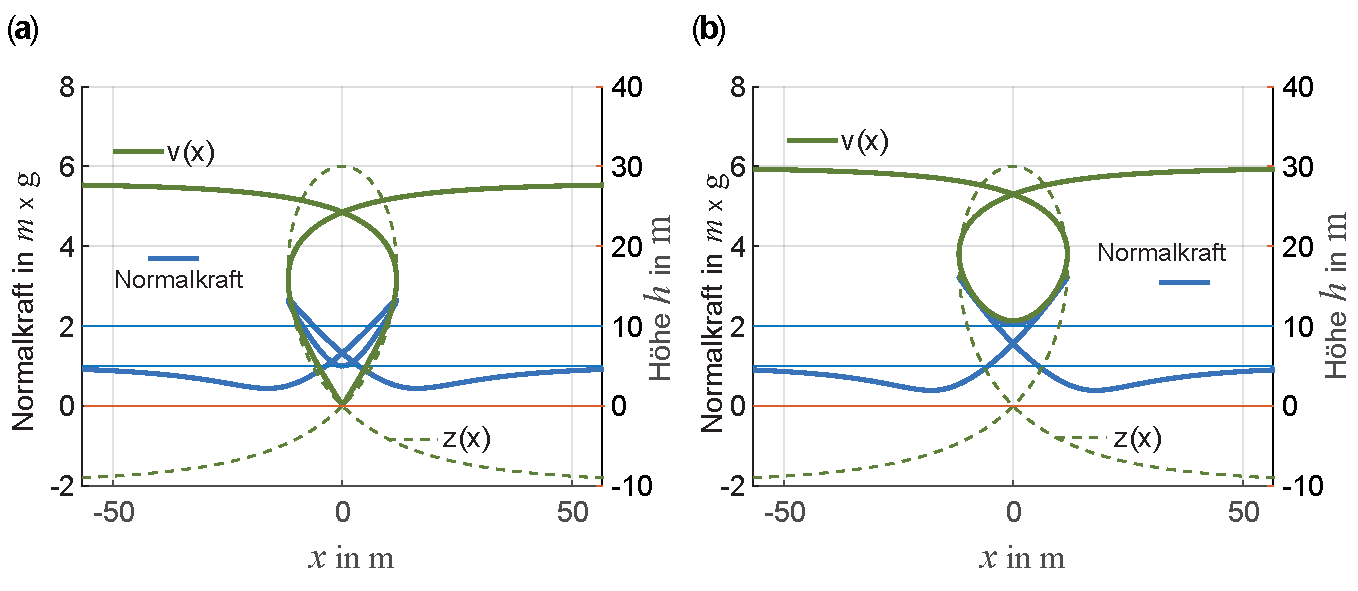
\includegraphics[width=\textwidth]{Achterbahn04.pdf}
  \caption[MacLaurin-Trisectrix als Beispiel f�r ein Looping.]{MacLaurin-Trisectrix als Beispiel f�r ein Looping.} \label{abb:bew_Achterbahn04}
\end{figure}

    \item [3)] \textit{\textbf{Bewegungsgleichung und Kr�fte auf die einzelnen Wagen in einem Zug, der eine beliebige Kurve durchf�hrt }}\\
		
\begin{figure}
  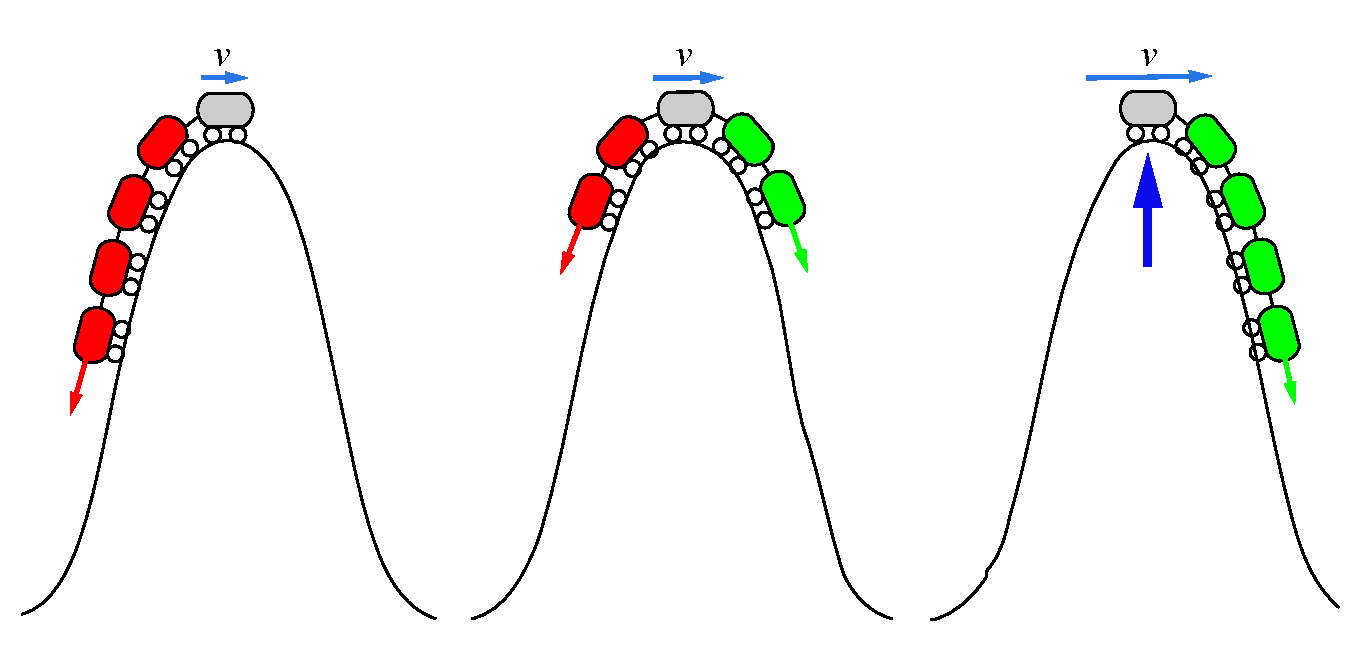
\includegraphics[width= \textwidth]{AchterbahnBergfahrt.pdf}
  \caption[Zug auf der Achterbahn - Bergfahrt]{Zug auf der Achterbahn  - Bergfahrt. Gezeigt ist die Fahrt �ber einen Berge ins n�chste Tal. Beschleunigende Wagen sind gr�n, bremsende rot gekennzeichnet. Der Pfeil zeigt die \textit{Airtime} an, die Insassen im letzten Wagen sp�ren, wenn sie den Berg �berfahren.} \label{abb:bew_AchterbahnZugBerg}
\end{figure}

\begin{figure}
  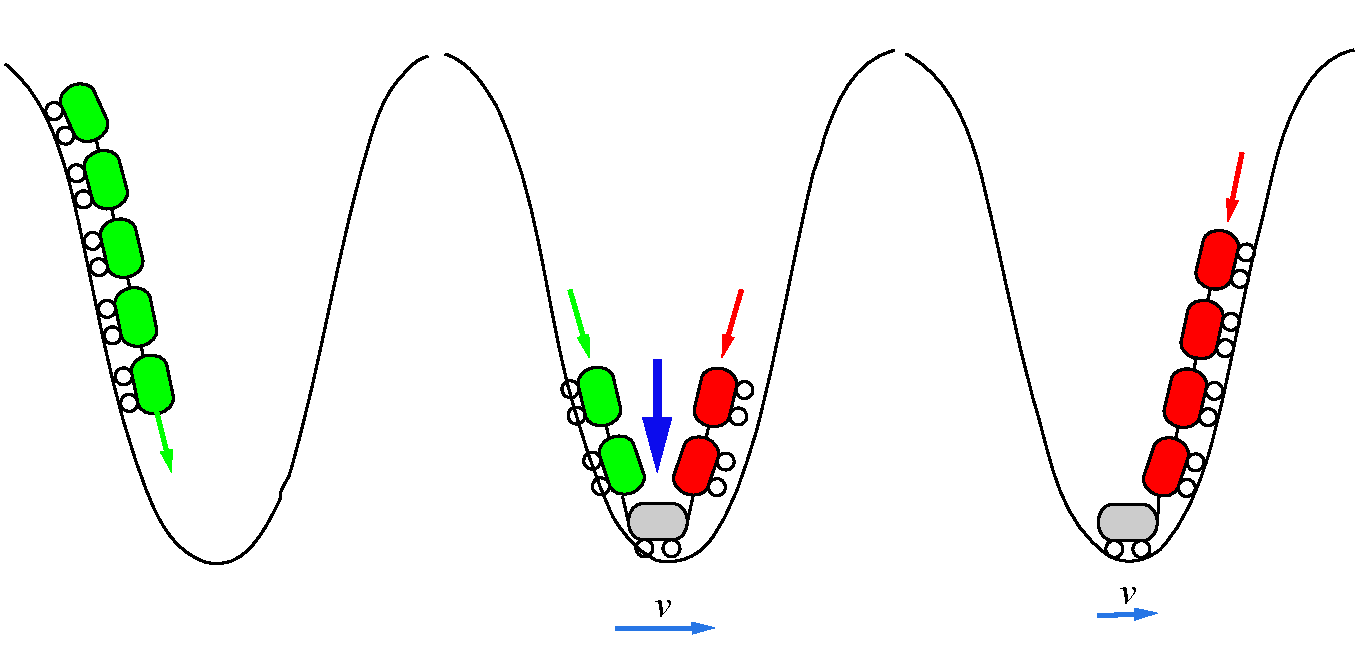
\includegraphics[width= \textwidth]{AchterbahnTalfahrt.pdf}
  \caption[Zug auf der Achterbahn - Talfahrt]{Zug auf der Achterbahn - Talfahrt. Gezeigt ist die Fahrt von einem Berge durch ein Tal auf den n�chsten Berg hinauf. Beschleunigende Wagen sind gr�n, bremsende rot gekennzeichnet. Der Pfeil zeigt die zus�tzliche Beschleunigung an, die Insassen im mittleren Wagen sp�ren, wenn sie das Tal durchfahren.} \label{abb:bew_AchterbahnZugTal}
\end{figure}

Wir wollen nun auch erkl�ren, warum die ersten und den letzten Wagen in einem Achterbahnzug am beliebtesten sind, abh�ngig davon ob man den gr��ten oder geringsten Nervenkitzel sp�ren m�chte. Zwischen den Wagen wirken zus�tzliche Kr�fte (Zug- und Schiebekr�fte). Obwohl alle Wagen eines Zuges zu jedem Zeitpunkt dieselbe Geschwindigkeit haben, kann die Geschwindigkeit, die ein Wagen an einem bestimmten Punkt der Bahn hat, sich jedoch durchaus von der eines anderen Wagens unterscheiden, als dieser am selben Ort war. Wir betrachten dazu \figref{bew_AchterbahnZugBerg}. Hier haben wir einen Achterbahnzug aus f�nf Wagen gezeichnet. Er befindet sich gerade auf dem Berg. Der erste Wagen beschleunigt mit seiner Gewichtskraft den gesamten Zug und mit jedem Wagen, der den Hochpunkt �berschreitet, nimmt die beschleunigende Kraft zu. Beim letzte Wagen auf der Bergkuppe  hat der Zug schon eine deutlich h�here Geschwindigkeit erreicht als zu dem Zeitpunkt als der erste Wagen auf der Bergkuppe war.  Auf den Mitfahrer im letzten Wagen wirkt deshalb eine h�here Zentrifugalbeschleunigung, er sp�rt also die gew�nschte Airtime intensiver als Mitfahrer in vorderen Wagen. Andere Verh�ltnisse gelten bei der Talfahrt \figref{bew_AchterbahnZugTal}. Wenn der mittlere Wagen den Tiefpunkt des Tals erreicht, befindet sich die vorderen Wagen schon wieder im Anstieg und wirken verz�gernd, die hinteren noch in der Abfahrt und wirken entsprechend beschleunigend auf den mittleren Wagen. Der mittlere Wagen durchf�hrt daher das Tal also mit der h�chsten Geschwindigkeit, auf ihn wirken deshalb die st�rksten positiven $g$-Kr�fte. Man kann leicht absch�tzen, dass in Achterbahnen kurzzeitig Beschleunigungen von bis zu $6 g$ auftreten k�nnen. Negativen $g$-Kr�fte l�sen bei den Passagieren das "`Kribbeln"' im Magen aus. 
Zur Behandlung des Problems im Lagrange-Formalismus wollen wir zun�chst die potentielle Energie des Zuges berechnen.
\begin{align}
    \text{Mit} ~~~z &= h\lk x\rk \,,~~ L = \int\limits_{x_\text{E}}^{x_\text{F}} \D s = \text{const}\,~~~M = \int\limits_{x_\text{E}}^{x_\text{F}}\mu\D s = \mu\,L \,~~~\text{findet man} \nonumber \\
    U\lk x_\text{F}\rk &=  g\,\int\limits_{x_\text{E}}^{x_\text{F}}\mu\,z\,\D s = g\,\mu\,\int\limits_{x_\text{E}}^{x_\text{F}} h\lk x\rk\,\sqrt{1 + h'\lk x\rk^2}\,\D x \,.\label{eq:bew_Achterbahn30}
\end{align}
Hierin ist $x_\text{F}$ die $x$-Position des Zugkopfes, $x_\text{E}$ die $x$-Position des Zugendes (\figref{bew_ZugKreisring}), $x_\text{F}$ ist unsere generalisierte Koordinate. 
Um $U\lk x_\text{F}\rk$ f�r die Lagrange-Funktion verwenden zu k�nnen, brauchen wir aber noch $x_\text{E} = x_\text{E}\lk x_\text{F},L\rk$. Dazu benutzen wir
\begin{align}
    \int\limits_{x_\text{E}}^{x_\text{F}}\D s &= \int\limits_{x_\text{E}}^{x_\text{F}}\sqrt{1+h'\lk x\rk^2}\,\D x = F\lk x_\text{F}\rk -F\lk x_\text{E}\rk = L \,.\label{eq:bew_Achterbahn31}
\end{align}

$F(x)$ ist die Stammfunktion von $\sqrt{1 + h'\lk x\rk^2}$ und ist i.A. nicht analytisch gegeben, $F^{-1}$ ist die inverse Funktion zu $F$, womit aus $F\lk x_\text{E}\rk = F\lk x_\text{F}\rk -L$ 
\begin{align}
    x_\text{E} &= F^{-1}\,\lk F\lk x_\text{F}\rk -L\rk \label{eq:bew_Achterbahn32}
\end{align}
folgt. Man kann $x_\text{E}$ zumindest numerisch berechnen, abh�ngig von $h'\lk x\rk$ eventuell auch analytisch. Die vorstehenden Rechnungen kann man auch f�r ein parametrisierte Kurve machen, f�r die gilt:
\begin{align}
    x &= x\lk u\rk  ~~~ x'\lk u\rk = \frac{\D x}{\D u} ~~~z= z\lk u\rk ~~~ z'\lk u\rk = \frac{\D z}{\D u}  \nonumber \\
    L &=  \int\limits_{t_E}^{t_F}\D s =  \int\limits_{t_E}^{t_F}\sqrt{\lk x'\rk^2 + \lk z'\rk^2}\, \D u \label{eq:bew_Achterbahn33}
\end{align}
Das Potential ergibt sich dann zu:
\begin{align}
    U = \mu\,g\,\int\limits_{u_E}^{u_F} z\lk u\rk\,\sqrt{x'{}^2 + z'{}^2} \,\D u \,.\label{eq:bew_Achterbahn34}
\end{align}
Mit Stammfunktion $F(u)$ erhalten wir wiederum eine Bestimmungsgleichung f�r $u_E$:
\begin{align}
    F\lk u\rk &= \int\sqrt{\lk x'\rk^2 + \lk z'\rk^2}\,\D u  ~~~\rightarrow ~~~~ F\lk u_F\rk - F\lk u_E\rk = L \nonumber \\
    \rightarrow ~~~~ u_E\lk u_F,L\rk &= F^{-1}\lk F\lk u_F\rk-L\rk\,.\label{eq:bew_Achterbahn35}
\end{align}

Wir k�nnen unsere Rechnungen leicht an einem Zug der L�nge $L$ in einem Kreis mit dem Radius $R$ �berpr�fen. Der Parameter $u$ ist dann der Winkel $\varphi$. Die einfachen Rechnung ergeben die bereits in Kap. \ref{kap:rollercoaster}
hergeleiteten Beziehungen \eqref{eq:bew_Achterbahn43a} und \eqref{eq:bew_Achterbahn43b}. 
Mit den Beziehungen \eqref{eq:bew_Achterbahn34} und \eqref{eq:bew_Achterbahn34} f�r die potentielle Energie k�nnen wir die Lagrange-Gleichungen erster Art \eqref{eq:bew_Achterbahn03} f�r die Koordinaten $x_\text{F}\,, z_F$ gehen.  Wir erhalten die L�sungen $x_\text{F}(t)\,, \dot{x}_F(t)\,, z_F(t)\,, \dot{z}_F(t)$. 
Damit ist auch f�r einen beliebigen Punkt (Wagen) im Zug $s_W(t)$, \dh $x_W(t)\,, z_W(t)$  die Geschwindigkeit $\dot{x}_W(t),\,, \dot{z}_W(t)$ bekannt, da die Kurvenform bekannt ist und der Betrag der Geschwindigkeit im gesamten Zug der Geschwindigkeit $v_F(t)$ entspricht. 
Aus der Kr�mmung der Kurve am Punkt $x_W(t)\,, z_W(t)$ des betrachteten Wagens kann man sich die Tangential- und Normalbeschleunigung bestimmen, ebenso nat�rlich die Kraftkomponenten aus dem Potential $\d U/\d x (x_W) \,, \d U/\d z (z_W)$, woraus man analog \eqref{eq:bew_Achterbahn11} die resultierenden Kr�fte $\vec{F}_\text{G} +\vec{F}_\text{N}$ auf den Wagen berechnen kann. Das ist numerisch etwas aufwendig, aber prinzipiell kein Problem.\\
Ein alternativer und sehr instruktiver Weg besteht darin, den Zug als Kette von einzelnen ($N$) Kettengliedern zu betrachten, die durch eine (harte) Feder gekoppelt sind. F�r das Problem kann man ein $2N$-dimensionales System von gekoppelten Bewegungsgleichungen aufstellen. Wir verweisen hierzu auf die \probref{bew_achterbahn_diskret}.\\

%
    %\item [4)] \emph{Bewegungsgleichung und Kr�fte auf die einzelnen Wagen in einem Zug, der einen Kreisring im Looping durchf�hrt} \\
%
%Bei der Behandlung des Problems m�ssen wir mehrere F�lle unterscheiden:
        %\begin{enumerate}
            %\item [1)] $L>2\pi\,R$ (Zugl�nge ist gr��er als Umfang der Loop)
						%\begin {enumerate}
						   %\item [a)] Zuganfang in der Loop, $\varphi_\text{F} > -\pi/2$ , dann Zugende au�erhalb der Loop,
						   %\item [b)] Zuganfang hat Loop durchfahren, $\varphi_\text{F} > 3\pi/2$,  Zugende noch au�erhalb der Loop,\\ Loop ist vollst�ndig durch Zug "`gef�llt"',
						   %\item [c)] Zuganfang hat Loop durchfahren und Zugende innerhalb der Loop,
            %\end{enumerate}
						%\item [2)] $L<2\pi\,R$ (Zugl�nge ist kleiner als Umfang der Loop)
						%\begin {enumerate}
						   %\item [a)] Zuganfang in der Loop und $\varphi_\text{F} < L/R$, Zugende au�erhalb der Loop,
						   %\item [b)] Zug ist komplett in der Loop $ L/R < \varphi_\text{F} <3\pi/2$,
						   %\item [c)] Zuganfang hat Loop durchfahren und Zugende noch innerhalb der Loop.
            %\end{enumerate}
        %\end{enumerate}

\end{enumerate}

\end{sol} 
%\href{PhysikUncut_Part1.pdf#prb:bew_achterbahn}{\textcolor{blue} {$\rightarrow$ zur \probref{bew_achterbahn}.}}\\
\textcolor{blue} {$\rightarrow$ zur} \probref{bew_achterbahn}.\\
\noindent\rule[1ex]{\textwidth}{0.5pt}  \newpage

%-----------------------------------------------------------------------------------------------------------
\newpage
\hypertarget{lsg:bew_achterbahn_diskret}{}
\begin{sol}{prob:bew_achterbahn_diskret}\label{lsg:bew_achterbahn_diskret} %�bung62
\textbf{Physik auf der Achterbahn II } \\ \\

Wir betrachten den Achterbahnzug als Kette von $N$ Wagen ($i = 1,2,\ldots,N$).
Dies erweitert den Ansatz aus Kapitel \ref{kap:rollercoaster} und �bung
\ref{prob:bew_achterbahn}, in dem der Zug aus einem Massepunkt bestand bestand.
Jeder Wagen wird wieder als Punktmasse angenommen und alle haben die identische
Masse $m$. Zwischen den Massepunkten wird die Kopplung durch eine (sehr) harte
Feder mit der Federkonstante $k$ angenommen. Die L�nge der Feder im entspannten
Zustand sei $s_0$, was dem Abstand von Wagenmittelpunkt zu Wagenmittelpunkt
entsprechen soll. Das entspricht der Darstellungen aus
\figref{bew_AchterbahnZugBerg} im \hyperref[lsg:bew_achterbahn]
{L�sungsvorschlag} zu �bung \probref{bew_achterbahn}. Genau den in dieser
Abbildung dargestellten Fall, die Berfahrt, wird in dieser �bung betrachtet.

Wir schreiben zun�chst das Potential auf und erhalten f�r sie Summe aus
der Lage- und Federspannenergie
\begin{align}
    U\lk \{x_i\},\{z_i\}\rk = m\,g\,\sum_{i=1}^{N}z_i + \frac{1}{2}\,k\sum_{i=1}^{N-1}\lk \sqrt{\lk x_{i+1}-x_i\rk^2 + \lk z_{i+1}-z_i\rk^2 }- s_0\rk^2 \,. \label{eq:bew_ABdiskret01}
\end{align}
Die geschweiften Klammern $\{\cdot\}$ sollen andeuten, dass alle $x_i$ und
$z_i$ im entsprechenden Term vorkommen. Die kinetische Gesamtenergie ergibt sich
aus der Summe der kinetischen Energien jedes einzelnen Wagens,
\begin{align}
    T\lk\{\dot{x}_i\},\{\dot{z}_i\}\rk = \frac{1}{2}\,m\sum_{i=1}^{N}\lk \dot{x}_i{}^2 + \dot{z}_i{}^2\rk\,.  \label{eq:bew_ABdiskret02}
\end{align}

In Verallgemeinerung der Nebenbedingung \eqref{eq:bew_Achterbahn00} f�r einen
einzelnen Massepunkt, die sich auf der Achterbahn bewegt, erhalten wir f�r
die $N$ Wagen die $N$ Nebenbedingungen
\begin{equation}
    f_i = z_i - h\lk x_i\rk = 0\,, \label{eq:bew_ABdiskret03}
\end{equation}
aus denen
\begin{align}
\begin{split}
  \dot{f}_i &= \dot{z}_i - \frac{\d h}{\d x_i}\,\dot{x}_i = 0 = \dot{z}_i
  - h'\,\dot{x}_i \,, \\
  \ddot{f}_i &= \ddot{z}_i - \frac{\d^2 h}{\d x_i^2}\,\dot{x}_i{}^2
  - \frac{\d h}{\d x_i}\,\ddot{x}_i = 0 = \ddot{z}_i - h''\,\dot{x}_i{}^2
  - h'\,\ddot{x}_i
\end{split} \label{eq:bew_ABdiskret04}
\end{align}
folgt.

Die $2N$ Bewegungsgleichungen (Lagrange-Gleichungen erster Art) lauten nach \eqref{eq:bew_Lagrange_I} dann
\begin{align}
\begin{split}
  \frac{\D}{\D t}\,\frac{\d \mathcal{L}}{\d \dot{x}_i} - \frac{\d \mathcal{L}}{\d x_i} &= m\,\ddot{x}_i + \frac{\d U}{\d x_i} = \sum_{n=1}^{N} \lambda_n\,\frac{\d f_n}{\d x_i} = \sum_{n=1}^{N} \delta_{ni}\,\lambda_n\,\frac{\d f_n}{\d x_i} = \lambda_i\,\frac{\d f_i}{\d x_i} \,, \\
    \frac{\D}{\D t}\,\frac{\d \mathcal{L}}{\d \dot{z}_i} - \frac{\d \mathcal{L}}{\d z_i} &= m\,\ddot{z}_i + \frac{\d U}{\d z_i} = \sum_{n=1}^{N} \lambda_n\,\frac{\d f_n}{\d z_i} = \sum_{n=1}^{N} \delta_{ni}\,\lambda_n\,\frac{\d f_n}{\d z_i} = \lambda_i\,\frac{\d f_i}{\d z_i} \,.
\end{split}  \label{eq:bew_ABdiskret05} 
\end{align}
Die einzelnen Massepunkte sind in den Bewegungsgleichungen �ber die Terme
$\d U/\d x_i$ \bzw $\d U/\d z_i$ verkoppelt. Wollen wir die
Bewegungsgleichungen explizit aufschreiben, m�ssen wir ber�cksichtigen, dass
der erste und letzte Wagen nur �ber eine Feder an einen anderen gekoppelt sind,
alle mittleren Wagen aber zwei Nachbarn haben. Dies f�hrt auf eine
Fallunterscheidung. F�r den ersten Wagen ($i=1$) gilt:
\begin{align}
    m\,\ddot{x}_1 &= - k\lk \sqrt{\lk x_2-x_1\rk^2 + \lk z_2-z_1\rk^2} -s_0\rk\,\frac{-2\lk x_2-x_1\rk}{2\,\sqrt{\lk x_2-x_1\rk^2 + \lk z_2-z_1\rk^2}} -\lambda_1\,h'\lk x_1\rk \notag\,,\\
                  &= -k\,\frac{\sqrt{\lk x_2-x_1\rk^2 + \lk z_2-z_1\rk^2} -s_0}{\sqrt{\lk x_2-x_1\rk^2 + \lk z_2-z_1\rk^2}}\,\lk x_2-x_1\rk - \lambda_1\,h'\lk x_1\rk\,, \notag \\
  m\,\ddot{z}_1 &= -k\,\frac{\sqrt{\lk x_2-x_1\rk^2 + \lk z_2-z_1\rk^2} -s_0}{\sqrt{\lk x_2-x_1\rk^2 + \lk z_2-z_1\rk^2}} \lk z_2 - z_1\rk -m\,g + \lambda_1 \,. \label{eq:bew_ABdiskret06}
\end{align}
Entsprechend gilt f�r den letzten Wagen ($i=N$):
\begin{align}
  m\,\ddot{x}_N &= -k \frac{\sqrt{\lk x_N - x_{N-1}\rk^2 + \lk z_N - z_{N-1}\rk^2} - s_0}{\sqrt{\lk x_N - x_{N-1}\rk^2 + \lk z_N - z_{N-1}\rk^2}}\,\lk x_N - x_{N-1}\rk - \lambda_N\,h'\lk x_N\rk \,, \notag \\
  m\,\ddot{z}_N &= -k \frac{\sqrt{\lk x_N - x_{N-1}\rk^2 + \lk z_N - z_{N-1}\rk^2} - s_0}{\sqrt{\lk x_N - x_{N-1}\rk^2 + \lk z_N - z_{N-1}\rk^2}}\,\lk z_N - z_{N-1}\rk - m\,g + \lambda_N\,.
                  \label{eq:bew_ABdiskret07}
\end{align}
F�r alle mittleren Wagen ($i=2,3,\ldots,N-1$) ergibt sich:
{ \allowdisplaybreaks
\begin{align}
  m\,\ddot{x}_i = \,&-k\, \frac{\sqrt{\lk x_i - x_{i-1}\rk^2 + \lk z_i- z_{i-1}\rk^2} - s_0}{\sqrt{\lk x_i - x_{i-1}\rk^2 + \lk z_i - z_{i-1}\rk^2}} \,\lk x_i -x_{i-1}\rk \notag \\
                    &+ k\, \frac{\sqrt{\lk x_{i+1} - x_i \rk^2 + \lk z_{i+1}- z_i \rk^2} - s_0}{\sqrt{\lk x_{i+1} - x_i \rk^2 + \lk z_{i+1} - z_i \rk^2}} \,\lk x_{i+1}-x_i\rk + \lambda_i\,h'\lk x_i\rk \,, \notag \\
  m\,\ddot{z}_i = \,&-k\, \frac{\sqrt{\lk x_i - x_{i-1}\rk^2 + \lk z_i- z_{i-1}\rk^2} - s_0}{\sqrt{\lk x_i - x_{i-1}\rk^2 + \lk z_i - z_{i-1}\rk^2}}\,\lk z_i - z_{i-1} \rk \notag \\
                    &+k\, \frac{\sqrt{\lk x_{i+1} - x_i \rk^2 + \lk z_{i+1}- z_i \rk^2} - s_0}{\sqrt{\lk x_{i+1}- x_i \rk^2 + \lk z_{i+1} - z_i \rk^2}}\,\lk z_{i+1} - z_i\rk -m\,g + \lambda_i\,.
                      \label{eq:bew_ABdiskret08}
\end{align}
}
Wir schreiben jetzt die Wurzelausdr�cke durch folgende Konvention etwas k�rzer:
\begin{align*}
  \sqrt{\lk x_i-x_j\rk^2 + \lk z_i-z_j\rk^2} = \Delta_{i,j}~~~\text{und f�r}~~~\frac{\Delta_{i,j}-s_0}{\Delta_{i,j}} = S_{i,j}\,.
\end{align*}

Die Lagrange-Multiplikatoren lassen sich nun bestimmen. Daf�r l�sen wir
zu jedem $i$ die Bewegungsgleichung f�r $z_i$ nach $\lambda_i$ auf, ersetzen
$\ddot{z}_i$ mit Hilfe der zugeh�rigen Nebenbedingung aus
\eqref{eq:bew_ABdiskret04} und sezten dort die Bewegungsgleichung f�r $x_i$
ein. Man erh�lt f�r $i=1$:
\begin{align}
    \lambda_1 &= m\,\ddot{z}_1 - k\,S_{2,1}\,\lk z_2-z_1\rk + m\,g \nonumber\\
    &= m\,h''\,\dot{x}_1{}^2 + m\,h'\,\ddot{x}_1 - k\,S_{2,1}\,\lk z_2-z_1\rk + m\,g \nonumber\\
    &= m\,h''\,\dot{x}_1{}^2 + h'\,k\,S_{2,1}\,\lk x_2-x_1\rk - h'^2\,\lambda_1 - k\,S_{2,1}\,\lk z_2-z_1\rk +m\,g \nonumber \,,\\
    \rightarrow ~~~~ \lambda_1 &= \frac{m\,g + m\,h''\,\dot{x}_1{}^2 + k\,S_{2,1}\lek h'\lk x_2-x_1\rk - \lk z_2-z_1\rk\rek}{1+h'{}^2}\,. \label{eq:bew_ABdiskret09}
\end{align}
F�r $i=N$ erh�lt man:
\begin{align}
    \rightarrow ~~~~ \lambda_N = \frac{m\,g + m\,h''\,\dot{x}_N{}^2 - k\,S_{N,N-1}\lek h'\lk x_N-x_{N-1}\rk - \lk z_N - z_{N-1}\rk\rek}{ 1+h'{}^2}\,. \label{eq:bew_ABdiskret10}
\end{align}
Schlie�lich ergibt sich f�r $i=2,3,\ldots,N-1$:
\begin{align}
\begin{split}
    \rightarrow ~~~~ \lambda_i =\,&\Bigg( m\,g + m\,h''\,\dot{x}_i{}^2 - k\,S_{i,i-1}\,\lek h'\lk x_i-x_{i-1}\rk - \lk z_i - z_{i-1}\rk\rek \\
    \,&+k\,S_{i+1,i} \,\lek h'\lk x_{i+1}-x_i\rk - \lk z_{i+1}-z_i\rk\rek\Bigg) \Bigg/\lk 1+h'{}^2\rk\,.
\end{split} \label{eq:bew_ABdiskret11}
\end{align}
Unser Modell wird eine gute N�herung f�r gro�e $N$ und damit kleine $s_0$
sein, wobei gilt:
\begin{equation*}
  M = \sum_{i=1}^{N}m = N\,m ~~~ \text{und}~~~L=N\,s_0\,.
\end{equation*}

Prinzipiell k�nnen wir die so erhaltenen $\lambda_i$, $i=1,\ldots,N$ in die
$2N$ Bewegungsgleichungen \eqref{eq:bew_ABdiskret06},
\eqref{eq:bew_ABdiskret07} und \eqref{eq:bew_ABdiskret08} einsetzen, um
die Lagrange-Multiplikatoren zu eliminieren. Die so erhaltenen Terme sind
jedoch sehr un�bersichtlich und bringen keinen Gewinn f�r das Verst�ndnis.
Wir berechnen die L�sungen numerisch und verwenden daf�r \mlbewref{Achterbahn04.m}.

Als Beispiel betrachten wir einen Zug aus 10 Wagen. Jeder Wagen soll die Masse
$m = \SI{500}{\kilo\gram}$ haben und ihr Abstand betrage in Ruhe $s_0 =
\SI{1}{\metre}$. Die Federkonstante habe den Wert $k=\SI{100}{\kilo\newton
  \per \metre}$. Die Bewegung finde auf der Gau�-Kurve
\eqref{eq:bew_Achterbahn06} mit einer H�he $h = \SI{30}{\metre}$ und einer
Breite $B=\SI{10}{\metre}$ statt.

Die Werte sind so gew�hlt, dass sie sinnvoll f�r eine Achterbahn sind, jedoch
kann man in weiteren Bereichen rechnen. Die Federn sind f�r die Wagen der
Masse $m = \SI{500}{\kilo\gram}$ recht hart, jedoch sind Bewegungen der Wagen
hier durchaus noch m�glich, wie in \figref{bew_AchterbahnD1} zu erkennen ist. 
Numerisch ist es kein Problem, die Federn deutlich h�rter (bis zu einem Faktor
1000 gr��er) zu w�hlen. Dann n�hert sich die Bewegung der einer starren
ausgedehnten Kette an. Harte Federn wollen wir annehmen, wenn $s$ vom
Eigengewicht eines Wages nicht um mehr als 10\% ver�ndert wird. Das bedeutet
$k > mg/(0{,}1\,s)$, was f�r die gew�hlten Parameter $k > \SI{50}{\kilo\newton
  \per \metre}$ bedeutet.

Im gew�hlten Fall finden Auslenkungen der Federn bis maximal $\SI{10}
{\centi\metre}$ statt. Dabei stellen sich Schwingungen ein, die auch nach Ende
der Fahrt noch erkennbar sind. Die rechte Abbildung zeigt die Geschwindigkeiten
des ersten und des letzten Wagens. Man erkennt wie diese zu unterschiedlichen
Zeiten ihren niedrigsten Wert erreichen.

\begin{figure}
\centering
  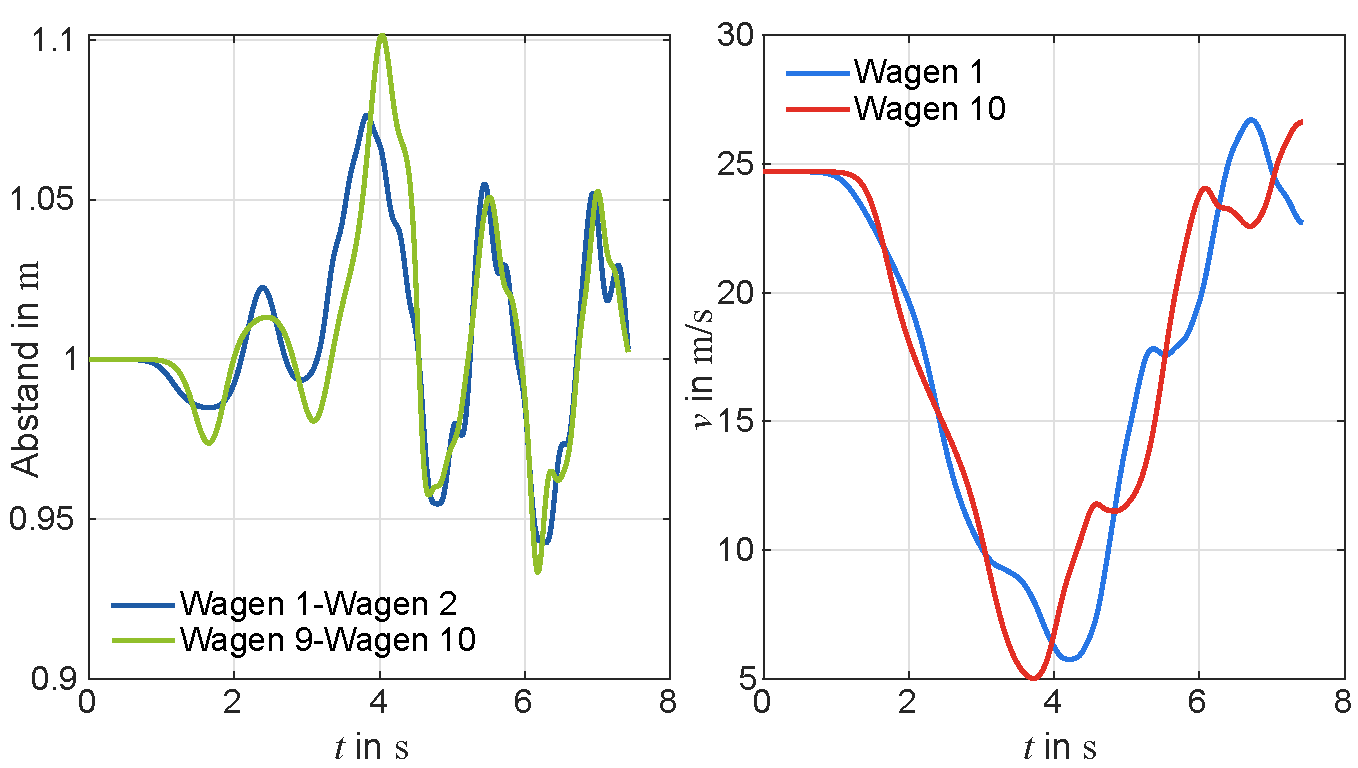
\includegraphics[width=\textwidth]{AchterbahnDiskret1.pdf}
  \caption[Gekoppelte Wagen auf einer Achterbahn]{Abst�nde (links) und
    Geschwindigkeiten (rechts) f�r ausgew�hlte Wagen eines Zuges aus $N=10$
    Wagen auf einer Achterbahn aus einer Gau�-Kurve.}
  \label{abb:bew_AchterbahnD1}
\end{figure}

Dies ist verst�ndlich, da der letzte Wagen, beeinflusst von seiner eigenen
Schwerkraft, die Feder dehnt, wenn der gr��te Teil des Zuges die Kuppe
bereits �berschritten hat, und dabei abbremst. Diese Feder beginnt dann jedoch,
ihn zu beschleunigen. Dies erkennt man ebenfalls sehr deutlich, wenn man die
Geschwindigkeit f�r verschiedene Wagen �ber dem Ort auftr�gt, wie es in
\figref{bew_AchterbahnD2} dargestellt ist. Wagen 10 nimmt seine
minimale Geschwindigkeit vor der Kuppe bei $x = \SI{0}{\metre}$ an.

\begin{figure}
  \centering
  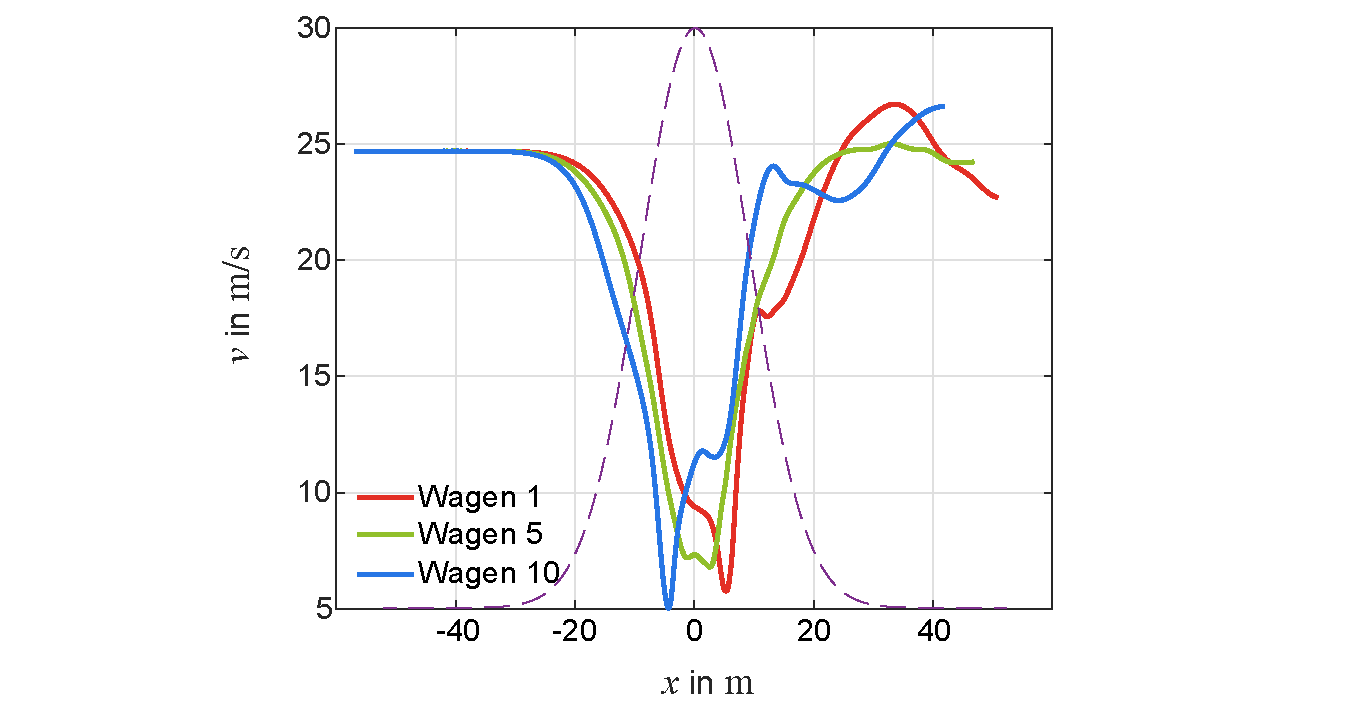
\includegraphics[width=\textwidth]{AchterbahnDiskret2.pdf}
  \caption[Geschwindigkeiten gekoppelter Wagen auf einer Achterbahn]
  {Geschwindigkeiten ausgew�hlter Wagen eines Zuges aus $N=10$ Wagen
    auf einer Achterbahn aus einer Gau�-Kurve in Abh�ngigkeit ihrer Position.
		Die Bahnkurve ist gestrichelt dargestellt.}
  \label{abb:bew_AchterbahnD2}
\end{figure}

Der erste Wagen erreicht seine minimale Geschwindigkeit jedoch erst hinter der
Kuppe. Durch die sich dehnenden Federn wird er weniger stark von den im
Anstieg befindlichen folgenden Wagen gebremst. Dies wird jedoch nachgeholt,
nachdem Wagen 1 sich im abfallenden Teil der Bahn befindet. In der
Zeitdarstellung aus \figref{bew_AchterbahnD1} findet man tats�chlich,
dass die Feder zwischen dem ersten und zweiten Wagen bei etwa $\SI{4}{\second}$
am st�rksten gedehnt ist, jedoch die minimale Geschwindigkeit von Wagen 1 erst
sp�ter erreicht wird. Es ist also hier tats�chlich die Feder, die nach der
Kuppe noch ein Abbremsen bewirkt.

\begin{figure}
  \centering
  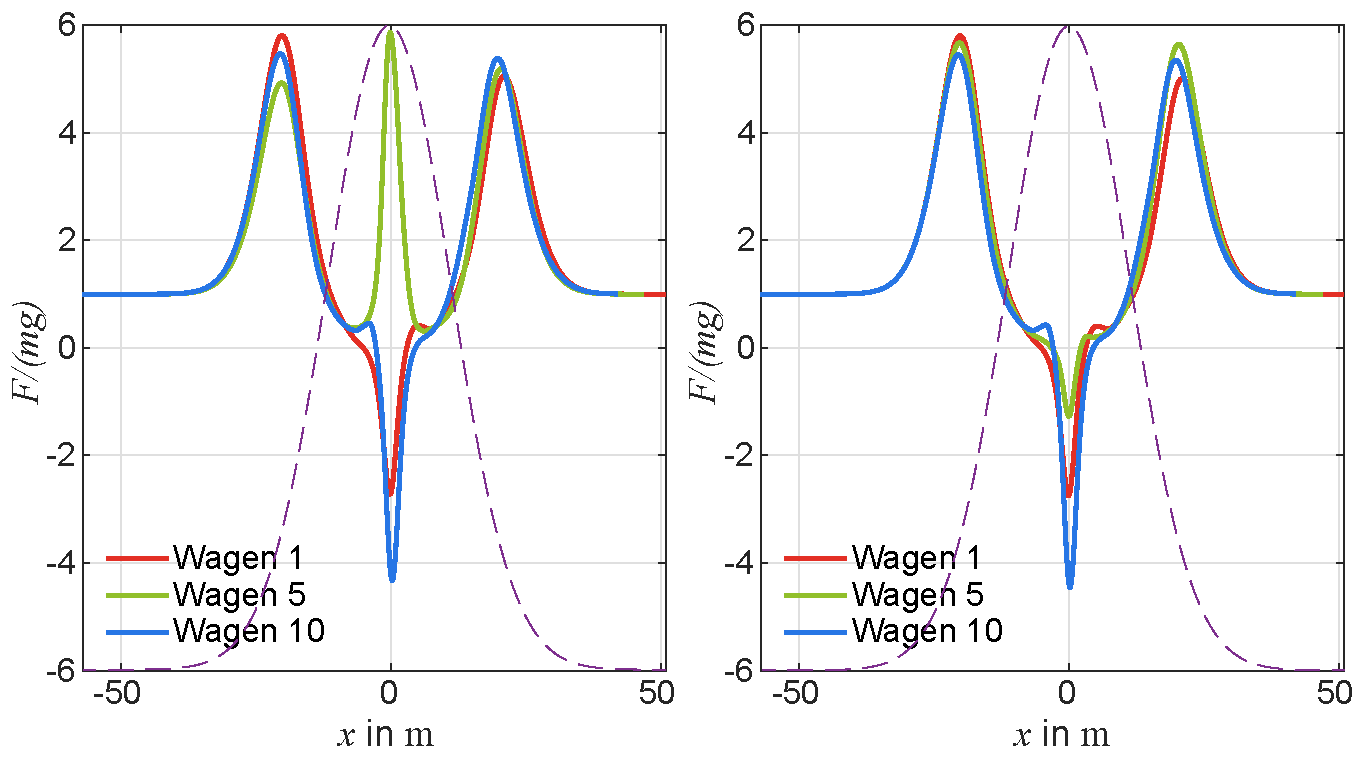
\includegraphics[width=\textwidth]{AchterbahnDiskret3.pdf}
  \caption[Normalkr�fte gekoppelter Wagen auf einer Achterbahn.]{Normalkr�fte
    ausgew�hlter Wagen (links) eines Zuges aus $N=10$ Wagen auf einer
    Achterbahn aus einer Gau�-Kurve sowie Normalkr�fte, die eine Person im
    Wagen erf�hrt (rechts). Die Bahnkurve ist gestrichelt dargestellt.} \label{abb:bew_AchterbahnD3}
\end{figure}

Schlie�lich betrachten wir noch die Normalkr�fte, die die Schienenf�hrung auf
einen Wagen aus�bt. Diese sind in \figref{bew_AchterbahnD3} linkst dargestellt.
Man erkennt deutlich, dass die �u�eren Wagen (hier 1 und 10) in der N�he der
Kuppe auf die Schienen gezogen werden m�ssen. Ihre Schwerkraft w�rde nicht
ausreichen, die n�tige Beschleunigung zu bewirken. Ganz anders ist das jedoch
f�r einen mittleren Wagen (hier der f�nfte), der, w�hrend er die Kuppe
passiert, so sehr von den anderen Wagen gezogen wird und deren Gewichtskraft
entgegenwirken muss, dass er auch in der Bewegung fest auf die Schienen dr�ckt.

Dies sagt jedoch nicht, welche Kraft eine Person im Wagen sp�rt. Dies ist
in \figref{bew_AchterbahnD3} rechts dargestellt. Dazu wurden alle Federkr�fte
in der Berechnung der Zwangskraft beseitigt, da die Person nicht mit
diesen verbunden ist. Hier stellt man fest, dass alle Personen, insbesondere
auch im mittleren Wagen, das Gef�hl des Abhebens haben, wenn sie die Kuppe
passieren. Aufgrund der unterschiedlichen Geschwindigkeiten der Wagen f�llt
dies jedoch unterschiedlich stark aus. Wie man in \figref{bew_AchterbahnD2}
sieht, hat aus den drei ausgew�hlten Wagen der letzte (Nummer 10) auf der
Kuppe die h�chste Geschwindigkeit und die Personen in ihm m�ssen durch die
st�rkste Kraft in der Bahn gehalten werden. Insbesamt werden jedoch die
Markierungen aus \figref{bew_AchterbahnZugBerg} im \hyperref[lsg:bew_achterbahn]
{L�sungsvorschlag} zu \probref{bew_achterbahn} best�tigt. Alle
Personen erleben eine Airtime. Diese ist, wie die Resultate ebenfalls zeigen,
f�r alle recht kurz und recht scharf um das Maximum der Kurve zentriert.
Dies ist nicht viel anders als f�r die Punktmasse aus \figref{bew_Achterbahn02}.
Der wesentliche Unterschied besteht darin, dass die Absolutwerte der
Normalbeschleunigungen f�r alle Wagen unterschiedlich sind.


\end{sol}

%\href{PhysikUncut_Part1.pdf#prb:bew_achterbahn_diskret}{\textcolor{blue} {$\rightarrow$ zur \probref{bew_achterbahn_diskret}.}}\\      
\textcolor{blue} {$\rightarrow$ zur} \probref{bew_achterbahn_diskret}.\\
\noindent\rule[1ex]{\textwidth}{0.5pt}  \clearpage

%-----------------------------------------------------------------------------------------------------------
\newpage
\hypertarget{lsg:bew_loop2loop}{}
\begin{sol}{prob:bew_loop2loop}\label{lsg:bew_loop2loop} %�bung63
\textbf{Physik auf der Achterbahn III} \\ \\

�berlegung zu auftretenden Beschleunigungen bei der Einfahrt:
\begin{figure}
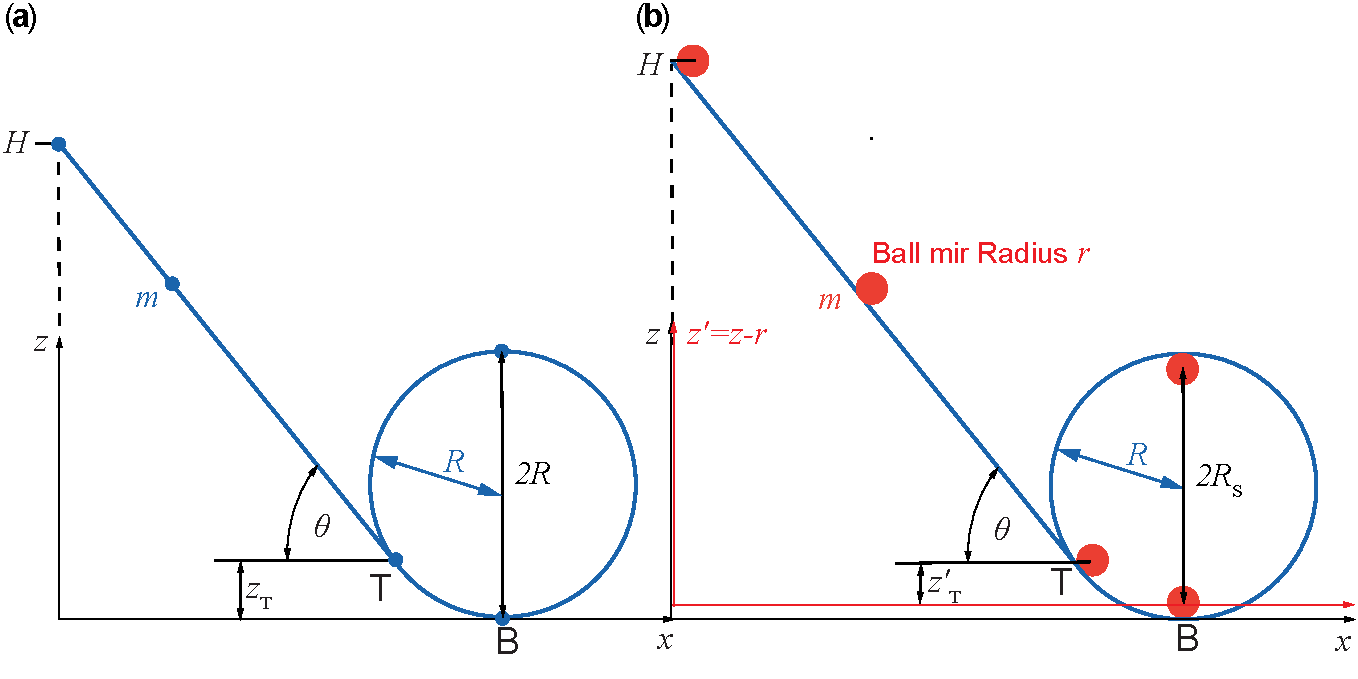
\includegraphics[width=\textwidth]{Loop2Loop.pdf}
\caption[Loop-the-Loop Problem]{\textit{Loop-the-Loop} Problem}\label{abb:bew_loop2loop2}
\end{figure}

Wir nehmen einen rollenden Ball mit Radius $r$ an. Sein Schwerpunkt hat auf der Geraden (Strecke von  $\mathrm{S}_0$ zu T) die Beschleunigung:
\begin{align}
    a = g\,\sin\vartheta - \frac{F_\text{R}}{m}\,, \label{eq:bew_loop01}
\end{align}
worin $F_\text{R}$ eine Reibungskraft sei. \\
Wir nehmen ferner reines Rollen an, dann kann die Rollbedingung $r'\,\omega = a$, worin $r'$ der effektive Radius zum Auflagepunkt des Balls ist\footnote{Der effektive Radius $r'$ kann von Radius $r$ abweichen, wenn \zb der Ball in einer V-f�rmigen Schiene rollt. Dann ist $r'<r$}, wie folgt verwendet werden:
\begin{align*}
    J\,\omega = F_\text{R}\,r' ~~~~ \rightarrow ~~~~ F_\text{R} = \frac{2}{5}\,m\,\frac{r^2}{r'{}^2}\,a\,.
\end{align*}
Damit erhalten wir f�r $r=r'$:
\begin{align}
\begin{split}
    a &= \frac{5}{7}\,g\,\sin\theta\,, \\
    F_\text{R} &= \frac{2}{7}\,m\,g\,\sin\theta\,.
\end{split} \label{eq:bew_loop02}
\end{align}
Am Punkt T wird der Ball einen abrupten Ruck (\textit{Jerk}) sp�ren und auch einen Energieverlust erfahren. \\
Dieser Energieverlust ist nur durch eine Kraft $F_\text{T}$ zu erkl�ren, die von einem komplexen Zusammenspiel von Ball und Unterlage am Punkt T herr�hrt und zu einem Energietransfer \zb in Form von Schwingungen auf die Unterlage f�hrt. Wir wollen nun diesen Energieverlust berechnen. \\
Wir k�nnen zun�chst die Energiebilanz f�r die Punkte S und T
\begin{align*}
    m\,g\,H = 2\,m\,g\,R_\text{S} + T + W_\text{R}\,,
\end{align*}
worin
\begin{align}
    T = \frac{1}{2}\,m\,v^2 + \frac{1}{2}\,J\,\omega^2 = \frac{7}{10}\,m\,v^2\,,
\end{align}
die kinetische Energie und $W_\text{R}$ die durch die Reibungskr�fte $F_\text{R}$ und $F_\text{T}$ \anf{geleistete} Arbeit ist. \\
In Abwesenheit von Reibungskr�ften w�rde aus der Bedingung an der Spitze des Loopings 
\begin{align*}
    \frac{v^2}{R_\text{S}} = g\,,
\end{align*}
dann eine minimale H�he $H$ f�r das Looping zu
\begin{align*}
    H = 2\,R_\text{S} + 0.7\,R_\text{S} = 2.7\,R_\text{S}
\end{align*}
folgen. Das ist etwas gr��er als die in \eqref{eq:bew_Achterbahn01} berechneten $H=2.5\,R$, was leicht durch die zus�tzliche Rotationsenergie des Balls zu erkl�ren ist. F�r die numerische Rechnung mit Reibung k�nnen wir die Bewegung in 3 Phasen unterteilen: \\

\textbf{\textit{Phase 1: Abrollen auf der schiefen Ebene
}}\begin{itemize}
    \item Anfangsbedingungen: $v_0 = 0$, $x_0 = 0$ , $z_0 =H$
    \item Endwerte: $v_\text{T}$, $x_\text{T}$, $z_\text{T}$
    \item In dieser Phase k�nnen wir auch einen Reibungskoeffizienten von \zb $\mu_\text{R} = 0.25 < \frac{2}{7}$ annehmen, so dass $F_\text{R}^{\lk 1\rk} = \mu_\text{R}^{\lk 1\rk}m\,g\,\cos\theta $ wird. Dann gilt nicht mehr reines Rollen. 
\end{itemize}
\textbf{\textit{Phase 2: Im Looping ab Tangentialpunkt T bis zum Boden der Loop (z=0) 
}}\begin{itemize}
    \item Anfangsbedingung: $v_\text{T}$, $x_\text{T}$, $z_\text{T}$
    \item F�r die Reibungskraft in dieser Phase nehmen wir einen erh�hten Wert nach $\mu_\text{R}^{\lk 2\rk} = 0.3$ an, so dass
    \begin{align*}
        F_\text{R}^{\lk 2\rk} = \mu_\text{R}^{\lk 2\rk}\,F_\text{N}^{\lk 2\rk} = \mu_\text{R}^{\lk 2\rk}\,\lk m\,g\,\cos\varphi + \frac{m\,v^2}{R_\text{S}}\rk
    \end{align*}
    Der erh�hte Koeffizient nimmt auch in Betracht, dass die Unterlage durch den Ruck eventuell schwingt und damit zus�tzlichen Energieverlust bewirkt. \\
    Diesen Energieverlust kann man genauer berechnen \cite{Mejia2020, Souza2017} oder durch eine Approximation modulieren \cite{Mamola2021}, was aber hier aus Platzgr�nden unterbleiben soll. Die numerische Integration ergibt die Endwerte: $v_\text{B}$, $x_\text{B}$, $z_\text{B}$
    \item F�r die numerische L�sung benutzen wir den in Kapitel \ref{kap:bew_Lagrange_I} behandelten oder alternativ den in Referenz \cite{Mamola2021} angegebenen Algorithmus.
\end{itemize}
\textbf{\textit{Phase 3: Vom Boden der Loop bis zur Spitze
}}\begin{itemize}
    \item Anfangsbedingungen: $v_\text{B}$, $x_\text{B}$, $z_\text{B}$
    \item Wir nehmen f�r dies Phase wieder reines Rollen an, so dass gilt:
    \begin{align*}
        \omega = \frac{a}{r} ~~~~ \text{und} ~~~~ J\,\omega = F_\text{R}\,r
    \end{align*}
\end{itemize}
Damit haben wir alle Parameter f�r die numerische Rechnung, die wir dem Leser als �bung �berlassen.
%Diese ist in \mlbewref{Loop2Loop.m} ausgef�hrt.

\end{sol} 
%\href{PhysikUncut_Part1.pdf#prb:bew_loop2loop}{\textcolor{blue} {$\rightarrow$ zur \probref{bew_loop2loop}.}}\\      
\textcolor{blue} {$\rightarrow$ zur} \probref{bew_loop2loop}.\\
\noindent\rule[1ex]{\textwidth}{0.5pt}  \newpage

%-----------------------------------------------------------------------------------------------------------
\newpage
\hypertarget{lsg:bew_achterbahn_vergleich}{}
\begin{sol}{prob:bew_achterbahn_vergleich}\label{lsg:bew_achterbahn_vergleich} %�bung64
  \textbf{Physik auf der Achterbahn IV} \\ \\

  Vergleich einer Kette aus Wagen mit dem kontinuierlichen Modell:
  Beim Aufstellen der Bewegungsgleichungen k�nnen wir auf
  \probref{bew_achterbahn_diskret} und die dort enthaltenen
  Bewegungsgleichungen \eqref{eq:bew_ABdiskret06} bis
  \eqref{eq:bew_ABdiskret08} zur�ckgreifen. Wir verzichten hier auf die
  Angabe des Lagrangeparameters, da die Gleichungen auch einfacher gefunden
  werden k�nnen. Trotzdem wollen wir uns eine gewisse Allgemeinheit bewahren,
  damit der interessierte Leser mit anderen Kurven weiterarbeiten kann. Wir
  gehen also erst einmal, wie in \probref{bew_achterbahn} nur davon aus, dass
  wir eine Parametrisierung $x(u)$, $z(u)$ vorliegen haben.

  Die umgeschriebenen Bewegungsgleichungen \eqref{eq:bew_ABdiskret06} bis
  \eqref{eq:bew_ABdiskret08} lauten mit einer allgemein gehaltenen Normalkraft
  $\vec{F}_N$ im Fall $i=1$:
  \begin{subequations}
    \begin{align}
      \ddot{x}_1 &= \frac{k}{m}\,\frac{\sqrt{\lk x_2-x_1\rk^2 + \lk z_2-z_1\rk^2} -s_0}{\sqrt{\lk x_2-x_1\rk^2 + \lk z_2-z_1\rk^2}}\,\lk x_2-x_1\rk - \frac{F_N}{m} \sin\vartheta_1\,, \label{eq:achterbahnvergleich01}\\
      \ddot{z}_1 &= \frac{k}{m}\,\frac{\sqrt{\lk x_2-x_1\rk^2 + \lk z_2-z_1\rk^2} -s_0}{\sqrt{\lk x_2-x_1\rk^2 + \lk z_2-z_1\rk^2}} \lk z_2 - z_1\rk -g + \frac{F_N}{m} \cos\vartheta_1 \,. \label{eq:achterbahnvergleich02}
    \end{align}
     Darin ist $\vartheta_1$ der Winkel, den die Tangente an die Bahn im
     aktuell betrachteten Punkt mit der $x$-Achse einschlie�t. Die Normalkraft
     steht senkrecht auf der Tangente. Entsprechend ergibt sich f�r den letzten
     Wagen ($i=N$):
\begin{align}
  m\,\ddot{x}_N &= -\frac{k}{m} \frac{\sqrt{\lk x_N - x_{N-1}\rk^2 + \lk z_N - z_{N-1}\rk^2} - s_0}{\sqrt{\lk x_N - x_{N-1}\rk^2 + \lk z_N - z_{N-1}\rk^2}}\,\lk x_N - x_{N-1}\rk - \frac{F_N}{m} \sin\vartheta_N \,, \\
  m\,\ddot{z}_N &= -\frac{k}{m} \frac{\sqrt{\lk x_N - x_{N-1}\rk^2 + \lk z_N - z_{N-1}\rk^2} - s_0}{\sqrt{\lk x_N - x_{N-1}\rk^2 + \lk z_N - z_{N-1}\rk^2}}\,\lk z_N - z_{N-1}\rk - m\,g + \frac{F_N}{m} \cos\vartheta_N \,.
\end{align}
F�r die mittleren Wagen ($i=2,3,\ldots,N-1$) notiert man:
{ \allowdisplaybreaks
\begin{align}
  m\,\ddot{x}_i = \,&-\frac{k}{m}\, \frac{\sqrt{\lk x_i - x_{i-1}\rk^2 + \lk z_i- z_{i-1}\rk^2} - s_0}{\sqrt{\lk x_i - x_{i-1}\rk^2 + \lk z_i - z_{i-1}\rk^2}} \,\lk x_i -x_{i-1}\rk \notag \\
                    &+ \frac{k}{m}\, \frac{\sqrt{\lk x_{i+1} - x_i \rk^2 + \lk z_{i+1}- z_i \rk^2} - s_0}{\sqrt{\lk x_{i+1} - x_i \rk^2 + \lk z_{i+1} - z_i \rk^2}} \,\lk x_{i+1}-x_i\rk - \frac{F_N}{m} \sin\vartheta_i \,, \\
  m\,\ddot{z}_i = \,&-\frac{k}{m}\, \frac{\sqrt{\lk x_i - x_{i-1}\rk^2 + \lk z_i- z_{i-1}\rk^2} - s_0}{\sqrt{\lk x_i - x_{i-1}\rk^2 + \lk z_i - z_{i-1}\rk^2}}\,\lk z_i - z_{i-1} \rk \notag \\
                    &+\frac{k}{m}\, \frac{\sqrt{\lk x_{i+1} - x_i \rk^2 + \lk z_{i+1}- z_i \rk^2} - s_0}{\sqrt{\lk x_{i+1}- x_i \rk^2 + \lk z_{i+1} - z_i \rk^2}}\,\lk z_{i+1} - z_i\rk -m\,g + \frac{F_N}{m} \cos\vartheta_N\,.
\end{align}
}
\end{subequations}

Um die Bewegungsgleichung f�r den Parameter $u$ zu erhalten, schreiben wir
die Parametrisierung aus,
\begin{align*}
  x_i &= x_i(u_i)\,, &\qquad z_i &= z_i(u_i)\,, \\
  \dot{x}_i &= x_i'(u_i)\,\dot{u}_i\,, &\qquad \dot{z}_i &= z_i'(u_i)\,\dot{u}_i
                                                         \,, \\
  \ddot{x}_i &= x_i''(u_i)\,\dot{u}_i^2 + x_i'(u)\,\ddot{u}_i\,,
                     &\qquad \ddot{z}_i &= z_i''(u_i)\,\dot{u}_i^2
                                          + z_i'(u_i)\,\ddot{u}_i \,. \\
\end{align*}

Exemplarisch l�sen wir f�r den Fall $i=1$ die Bewegungsgleichungen
\eqref{eq:achterbahnvergleich01} und \eqref{eq:achterbahnvergleich02}
nach der f�r $u_1$ auf. Dazu schreiben wir f�r \eqref{eq:achterbahnvergleich01}
\begin{align*}
  \ddot{x}_1 &= x_1''(u_1)\dot{u}_1^2 + x_1'(u)\ddot{u}_1 \\
             &= \frac{k}{m}\,\frac{\sqrt{\lk x_2-x_1\rk^2 + \lk z_2-z_1\rk^2} -s_0}{\sqrt{\lk x_2-x_1\rk^2 + \lk z_2-z_1\rk^2}}\,\lk x_2-x_1\rk - \frac{F_N}{m} \cos\vartheta_1 \tan\vartheta_1
\end{align*}
Den Term f�r die Normalkraft haben wir gleich so umgeschrieben, dass wir
\eqref{eq:achterbahnvergleich02} nach dieser aufl�sen und hier einsetzen k�nnen.
{\allowdisplaybreaks
\begin{align*}
  \ddot{x}_1 &= x_1''(u_1)\dot{u}_1^2 + x_1'(u)\ddot{u}_1 \\
             &= \frac{k}{m}\,\frac{\sqrt{\lk x_2-x_1\rk^2 + \lk z_2-z_1\rk^2} -s_0}{\sqrt{\lk x_2-x_1\rk^2 + \lk z_2-z_1\rk^2}}\,\lk x_2-x_1\rk \\
             &- \tan\vartheta_1 \left [ \ddot{z}_1 -  \frac{k}{m}\,\frac{\sqrt{\lk x_2-x_1\rk^2 + \lk z_2-z_1\rk^2} -s_0}{\sqrt{\lk x_2-x_1\rk^2 + \lk z_2-z_1\rk^2}}\,\lk z_2-z_1\rk + g \right ] \\
             &= \frac{k}{m}\,\frac{\sqrt{\lk x_2-x_1\rk^2 + \lk z_2-z_1\rk^2} -s_0}{\sqrt{\lk x_2-x_1\rk^2 + \lk z_2-z_1\rk^2}}\,\lk x_2-x_1\rk \\
  &- \tan\vartheta_1 \left [ z_1''(u_1)\dot{u}_1^2 + z_1'(u)\ddot{u}_1 -  \frac{k}{m}\,\frac{\sqrt{\lk x_2-x_1\rk^2 + \lk z_2-z_1\rk^2} -s_0}{\sqrt{\lk x_2-x_1\rk^2 + \lk z_2-z_1\rk^2}}\,\lk z_2-z_1\rk + g \right ]
\end{align*}
}
Ber�cksichtigt man nun noch, dass
\begin{equation*}
  \tan\vartheta = \frac{z'}{x'}\; ,
\end{equation*}
so l�sst sich dies aufl�sen zu
\begin{multline*}
  \ddot{u}_1 = \Bigg [ -\left(x_1'\,x_1''+ z_1'\,z_1'' \right ) \dot{u}_1^2
  + \frac{k}{m}\,\frac{\sqrt{\lk x_2-x_1\rk^2 + \lk z_2-z_1\rk^2} -s_0}{\sqrt{\lk x_2-x_1\rk^2 + \lk z_2-z_1\rk^2}}\,\lk x_2-x_1\rk x_1' \\
  + \frac{k}{m}\,\frac{\sqrt{\lk x_2-x_1\rk^2 + \lk z_2-z_1\rk^2} -s_0}{\sqrt{\lk x_2-x_1\rk^2 + \lk z_2-z_1\rk^2}}\,\lk z_2-z_1\rk z_1' - g z_1' \Bigg ]
/ \left ( x_1'^2 + z_1'^2 \right ) \; .
\end{multline*}
Ganz analog berechnet man im Fall $i=N$
\begin{multline*}
  \ddot{u}_N = \Bigg [ -\left(x_N'\,x_N''+ z_N'\,z_N'' \right ) \dot{u}_N^2\\
  - \frac{k}{m}\,\frac{\sqrt{\lk x_N-x_{N-1}\rk^2 + \lk z_N-z_{N-1}\rk^2} -s_0}{\sqrt{\lk x_N-x_{N-1} \rk^2 + \lk z_N-z_{N-1} \rk^2}}\,\lk x_N-x_{N-1} \rk x_N' \\
  - \frac{k}{m}\,\frac{\sqrt{\lk x_N-x_{N-1}\rk^2 + \lk z_N-z_{N-1}\rk^2} -s_0}{\sqrt{\lk x_N-x_{N-1} \rk^2 + \lk z_N-z_{N-1} \rk^2}}\,\lk z_N-z_{N-1} \rk z_N' - g z_N' \Bigg ]  / \left ( x_N'^2 + z_N'^2 \right )
\end{multline*}
und f�r die mittleren Wagen ($i=2,3,\ldots,N-1$)
{\allowdisplaybreaks
\begin{multline*}
  \ddot{u}_i = \Bigg [ -\left(x_i'\,x_i''+ z_i'\,z_i'' \right ) \dot{u}_i^2 \\
  - \frac{k}{m}\,\frac{\sqrt{\lk x_i-x_{i-1}\rk^2 + \lk z_i-z_{i-1}\rk^2} -s_0}{\sqrt{\lk x_i-x_{i-1} \rk^2 + \lk z_i-z_{i-1} \rk^2}}\,\lk x_i-x_{i-1} \rk x_i' \\
  + \frac{k}{m}\,\frac{\sqrt{\lk x_{i+1}-x_i\rk^2 + \lk z_{i+1}-z_i\rk^2} -s_0}{\sqrt{\lk x_{i+1}-x_i \rk^2 + \lk z_{i+1}-z_i \rk^2}}\,\lk x_{i+1}-x_i \rk x_i' \\
  - \frac{k}{m}\,\frac{\sqrt{\lk x_i-x_{i-1}\rk^2 + \lk z_i-z_{i-1}\rk^2} -s_0}{\sqrt{\lk x_i-x_{i-1} \rk^2 + \lk z_i-z_{i-1} \rk^2}}\,\lk z_i-z_{i-1} \rk z_i' \\
  + \frac{k}{m}\,\frac{\sqrt{\lk x_{i+1}-x_i\rk^2 + \lk z_{i+1}-z_i\rk^2} -s_0}{\sqrt{\lk x_{i+1}-x_i \rk^2 + \lk z_{i+1}-z_i \rk^2}}\,\lk z_{i+1}-z_i \rk z_i' - g z_i' \Bigg ] / \left ( x_i'^2 + z_i'^2 \right ) \; .
\end{multline*}
}

In dieser Aufgabe wollen wir den Kreislooping untersuchen, die zugeh�rige
Parametrisierung lautet
\begin{equation*}
  x_i = R \sin(\varphi_i) \; , \qquad x_i = R \lk 1- \cos(\varphi_i) \rk 
\end{equation*}
mit dem Parameter $u_i = \varphi_i$.
In \mlbewref{Achterbahn06.m}
befindet sich ein Programm, dass diesen Satz an Differentialgleichungen f�r
den Kreislooping l�st. Es berechnet ebenfalls die Bewegung eines starren
kontinuierlichen Zuges nach der Bewegungsgleichung
\eqref{eq:bew_Achterbahn45b} aus Kapitel \ref{kap:rollercoaster} und
erm�glicht so einen Vergleich beider Modelle.

Wir w�hlen als Beispiel einen Zug aus 5 Wagen mit denselben Parametern
wie in \probref{bew_achterbahn_diskret}. Dieses Beispiel ist in 
\figref{bew_AchterbahnKreis1} dargestellt. Man sieht in der linken
Abbildung deutlich, dass sich der Abstand zwischen zwei Wagen �ndern
kann. Mit dieser Federh�rte ist es den Federn m�glich, sich zu Dehnen und zu
stauchen. Dieser Effekt ist im starren, kontinuierlichen Modell aus
Kapitel \ref{kap:rollercoaster} nat�rlich nicht enthalten und eine
Abweichung beider Modelle ist zu erwarten. Diese ist in der rechten Abbildung
f�r die Geschwindigkeiten als Funktion der Zeit aufgetragen, weil hier der
Vergleich am besten m�glich ist. Die Abweichungen sind deutlich zu erkennen.
Keiner der beiden Wagen hat denselben Verlauf der Geschwindigkeit wie das
kontinuierliche Modell. Trotzdem ist die �bereinstimmung aber sehr gut.
Die einzelnen Wagen bewegen sich sehr nahe am Verlauf des starren, ausgedehnten
Zuges.

\begin{figure}
  \centering
  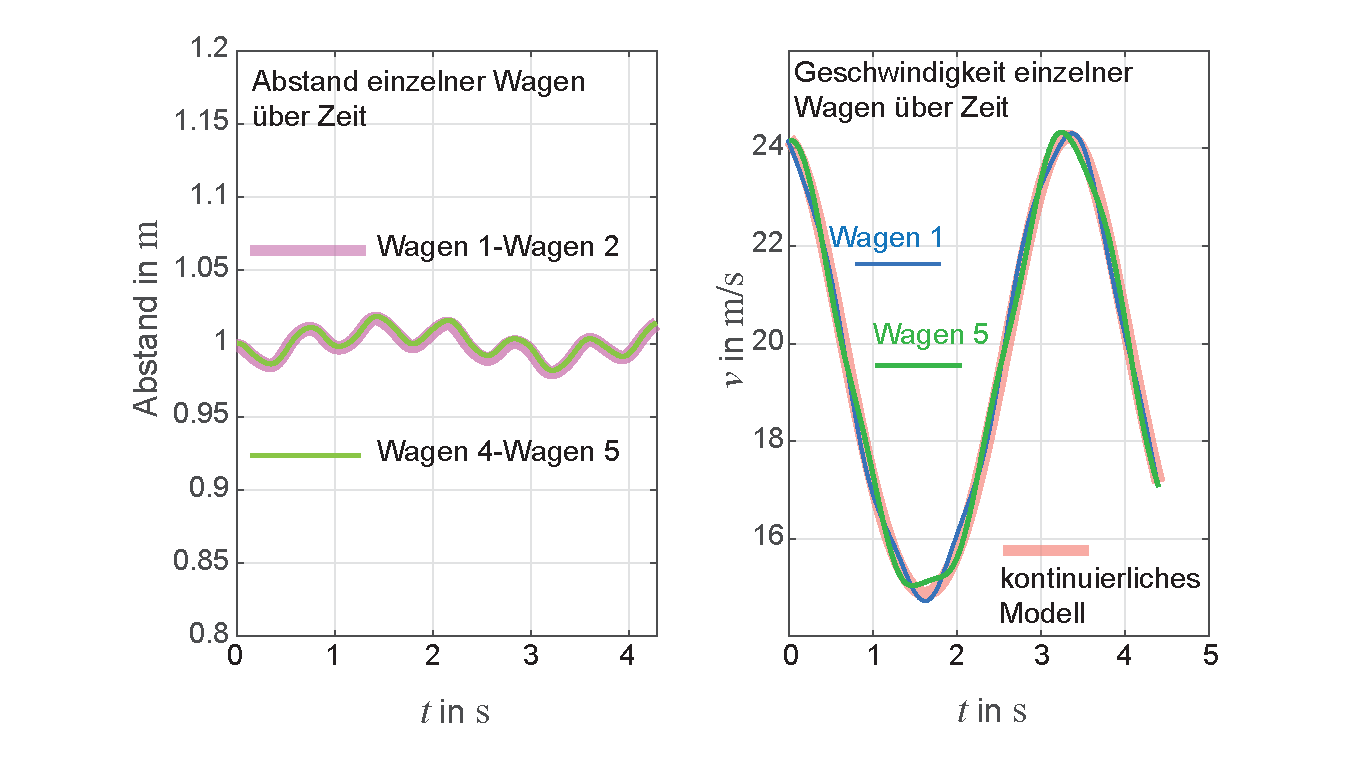
\includegraphics[width=\textwidth]{AchterbahnKreis01.pdf}
  \caption[Achterbahnzug auf einem Kreislooping, Federn des Zugs beansprucht]
  {Bewegung eines Achterbahnzuges auf einem Kreislooping, wobei die Parameter
    so gew�hlt sind, dass die Federn des Zuges aus f�nf Massepunkten beansprucht
    werden. Abweichungen zum starren, kontinuierlichen Modell sind erkennbar.}
  \label{abb:bew_AchterbahnKreis1}
\end{figure}
\begin{figure}
  \centering
  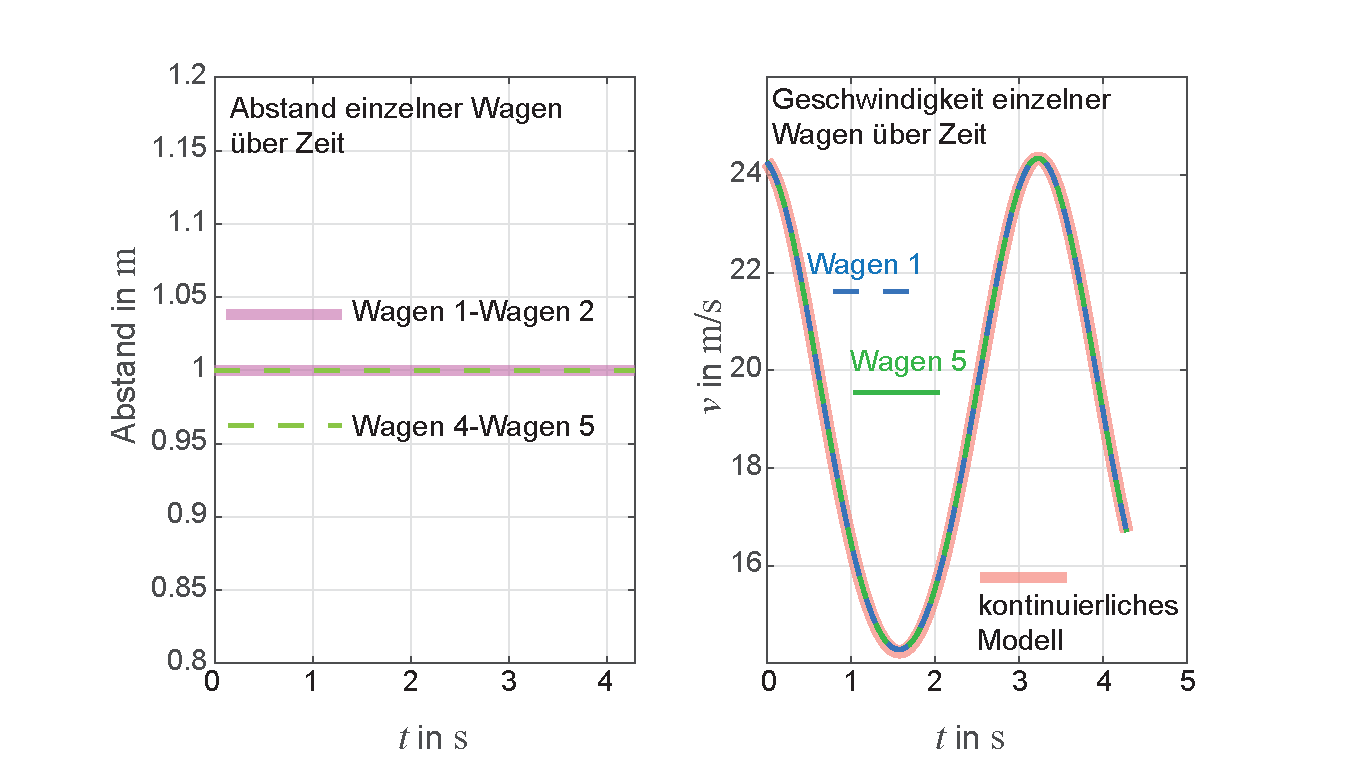
\includegraphics[width=\textwidth]{AchterbahnKreis02.pdf}
  \caption[Achterbahnzug, Federn des Zugs nicht beansprucht]{Bewegung eines Achterbahnzuges auf einem Kreislooping, wobei
    die Federh�rten so eingsellt sind, dass die Federn von den auftretenden
    Kr�ften nahezu nicht bewegt werden k�nnen. Die �bereinstimmung mit
    dem starren, kontinuierlichen Modell ist sehr hoch.}
  \label{abb:bew_AchterbahnKreis2}
\end{figure}

Stellt man die Federh�rte k�nstlich so ein, dass die Federn von den
auftretenden Kr�ften kaum noch aus ihrer Ruhel�nge gedehnt oder gestaucht
werden k�nnen, sollten die beiden Modelle sich nicht mehr signifikant
unterscheiden, da sich nun auch das diskrete Modell wie f�nf starr miteinander
verbundene Massepunkte verh�lt. Tats�chlich findet man kaum Unterschiede
in beiden L�sungen. Ein Beispiel ist in \figref{bew_AchterbahnKreis2}
gegeben. Die Parameter wurden wie in Abbildung \figref{bew_AchterbahnKreis1}
gew�hlt, jedoch mit einer um den Faktor 1000 gr��eren Federkonstante. Man
erkennt, dass die Wagen stets konstante Abst�nde zueinander einhalten. Die
Geschwindigkeiten der beiden ausgew�hlten Wagen und des Zuges aus dem
kontinuierlichen Modell liegen exakt aufeinander.\\
F�r den hier behandelten sehr einfachen Kreis ist es also nur wichtig, dass
die Massepunkte starr miteinander verbunden sind, um ein Verhalten zu sehen,
dass dem kontinuierlichen Modell sehr �hnlich ist. Es ist nicht entscheidend,
einen Kontinuums-�bergang mit sehr vielen Wagen in sehr kurzen Abst�nden
durchzuf�hren. Wird die Kurvenform jedoch komplizierter, k�nnen mit den
f�nf hier gew�hlten Wagen deutlichere Abweichungen auftreten, da das
kontinuierliche Modell stets die gesamte Kurvenform (und damit den gesamten
Potentialverlauf) �ber die L�nge des Zuges sieht, w�hrend die diskreten
Massepunkte, selbst wenn sie starr miteinander verbunden sind, nur punktuell
das Potential sehen und der Verlauf dazwischen irrelevant ist.
  
\end{sol} 
%\href{PhysikUncut_Part1.pdf#prb:bew_achterbahn_vergleich}{\textcolor{blue} {$\rightarrow$ zur \probref{bew_achterbahn_vergleich}.}}\\      
\textcolor{blue} {$\rightarrow$ zur} \probref{bew_achterbahn_vergleich}.\\
\noindent\rule[1ex]{\textwidth}{0.5pt}  

%-----------------------------------------------------------------------------------------------------------
\newpage
\hypertarget{lsg:bew_Trebuchet}{}
\begin{sol}{prob:bew_Trebuchet}\label{lsg:bew_Trebuchet} %�bung65
\textbf{Steinschleuder (\textit{Floating Arm Trebuchet} I)} \\ 

\begin{figure}[H]\centering
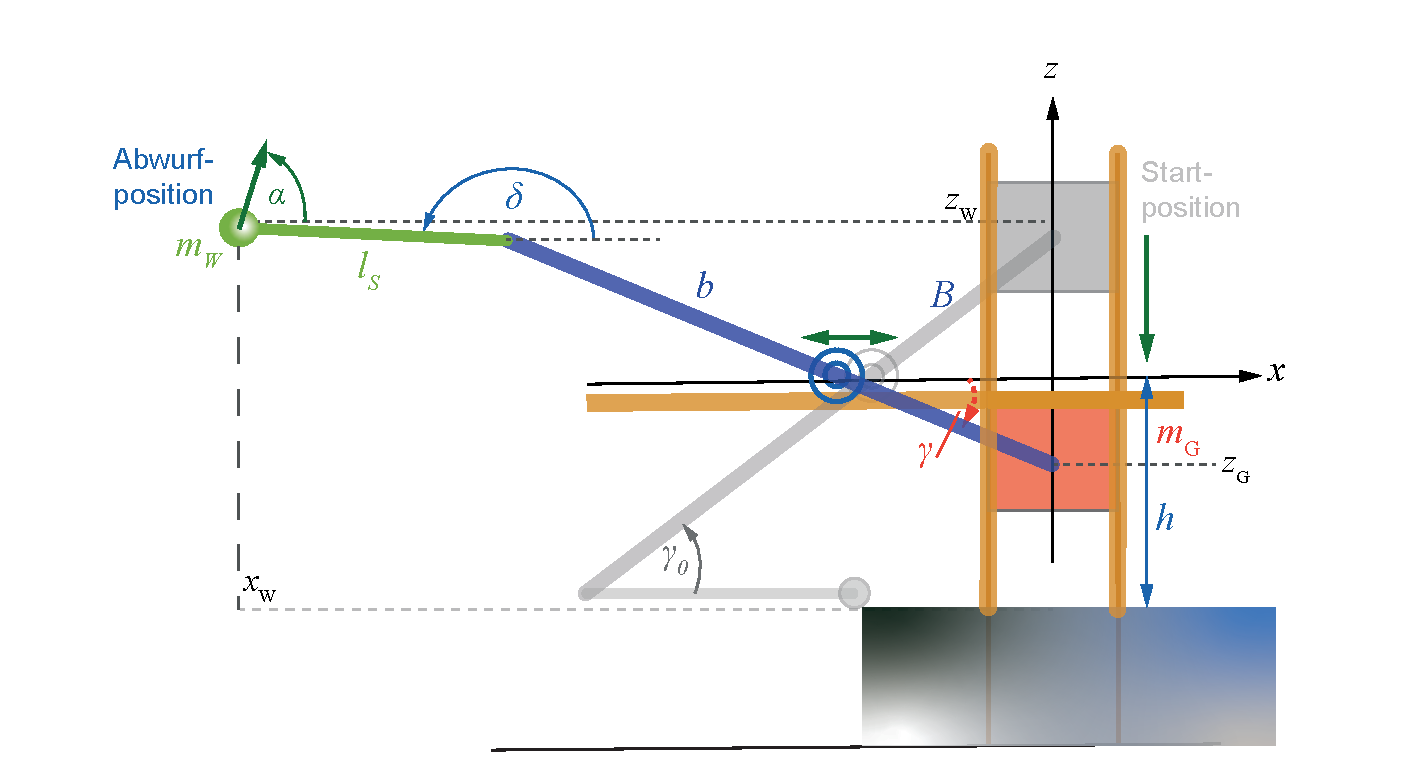
\includegraphics[width=\textwidth]{FloatArmTreb01.pdf}
\caption[Floating Arm Trebuchet als Variante einer mittelalterliche Wurfmaschine]{\textit{Floating Arm Trebuchet} als Variante einer mittelalterliche Wurfmaschine (Trebuchet, Blide). Geometrie und physikalische Gr��en.} 
\label{abb:bew_FloatArmTreb01a}
\end{figure}

Die Geometrie des \textit{Floating Arm Trebuchet} ist in \figref{bew_FloatArmTreb01a} zu sehen.
Wir leiten daraus die Ortsvektoren des Wurfgeschosses und des Gelenks als Funktion der Winkel $\gamma$ und $\delta$ ab: 
\begin{equation*}
	\begin{pmatrix}
			x_\text{W}\\
			z_\text{W}
	\end{pmatrix}
	=
	\begin{pmatrix}
			-(b+B)\,\cos\gamma + l_\text{S} \,\cos\delta\\
			-b\,\sin\gamma + l_\text{S} \,\sin\delta
	\end{pmatrix}\,,
\end{equation*}		
\begin{equation*}
	\begin{pmatrix}
			x_\text{G}\\
			z_\text{G}
	\end{pmatrix}
	=
	\begin{pmatrix}
			0\\
			+B\,\sin\gamma
	\end{pmatrix}\,.
\end{equation*}	
Die Geschwindigkeitsvektoren ergeben sich zu
\begin{equation*}
	\begin{pmatrix}
			\dot{x}_\text{W}\\
			\dot{z}_\text{W}
	\end{pmatrix}
	=
	\begin{pmatrix}
			+(b+B) \, \dot{\gamma}\sin\gamma - l_\text{S} \, \dot{\delta} \, \sin\delta\\
			-b \, \dot{\gamma} \, \cos\gamma + l_\text{S} \, \dot{\delta} \, \cos\delta 
	\end{pmatrix}\,,
\end{equation*}		
\begin{equation*}
	\begin{pmatrix}
			\dot{x}_\text{G}\\
			\dot{z}_\text{G}
	\end{pmatrix}
	=
	\begin{pmatrix}
			0\\
			-B\,\dot{\gamma}\,\cos\gamma 
	\end{pmatrix}\,.
\end{equation*}
Die Lagrange-Funktion $\mathcal{L}$ ist wieder die Differenz von $T$ und $U$:
		\begin{align*}
				T &= \frac{m_\text{G}}{2}\,\dot{z}_\text{G}{}^2 + \frac{J_\text{T}}{2}\,\dot{\gamma}^2 + \frac{m_\text{W}}{2}\lek \dot{x}_\text{W}{}^2 + \dot{z}_\text{W}{}^2\rek\\
				&= \frac{m_\text{G}}{2} \lk B\,\dot{\gamma}\,\cos\gamma \rk^2+ \frac{1}{2}\,J_\text{T} \,\dot{\gamma}^2 + \ldots \\
				&\quad +\quad\frac{m_\text{W}}{2} \lek \lk (B+b) \, \dot{\gamma}\,\sin\gamma - l_\text{S}\, \dot{\delta}\,\sin\delta \rk^2 + 
				\lk b \, \dot{\gamma}\,\cos\gamma - l_\text{S} \,\dot{\delta}\,\cos\delta  \rk^2 \rek \,, \\
				U &=  m_\text{G} \, g \, z_\text{G} + m_\text{W} \, g\, z_\text{W} - \frac{m_\text{T}}{2}\,g\,(b-B) \\
				&= g \lek m_\text{G} \, B - m_\text{W}\, b\rek \sin\gamma + g \, m_\text{W}\, l_\text{S}\,\sin\delta - \frac{m_\text{T}}{2}\,g\,(b-B) \,.
		\end{align*}
Hierin sind $m_\text{T}$ das Gewicht des Balkens und $J_\text{T}$ sein Tr�gheitsmoment bez�glich der Rolle. 
Die Anfangsbedingungen f�r die beiden verallgemeinerten Koordinaten $\gamma$ und $\delta$ lauten:
	\begin{equation*}
			\gamma_0 = +\arcsin{\lk\frac{h}{b}\rk} \,, 
			\qquad 
			\dot{\gamma}_0 = 0\,,
			\qquad
			\delta_0 = 0 \,, 
			\qquad
			\dot{\delta}_0 = 0 \,. 
	\end{equation*}

%%%%%%%%%%%%%
\begin{subprobs}
	\subprob{Ohne Zwangsbedingungen}

		\begin{figure}[H]\centering
		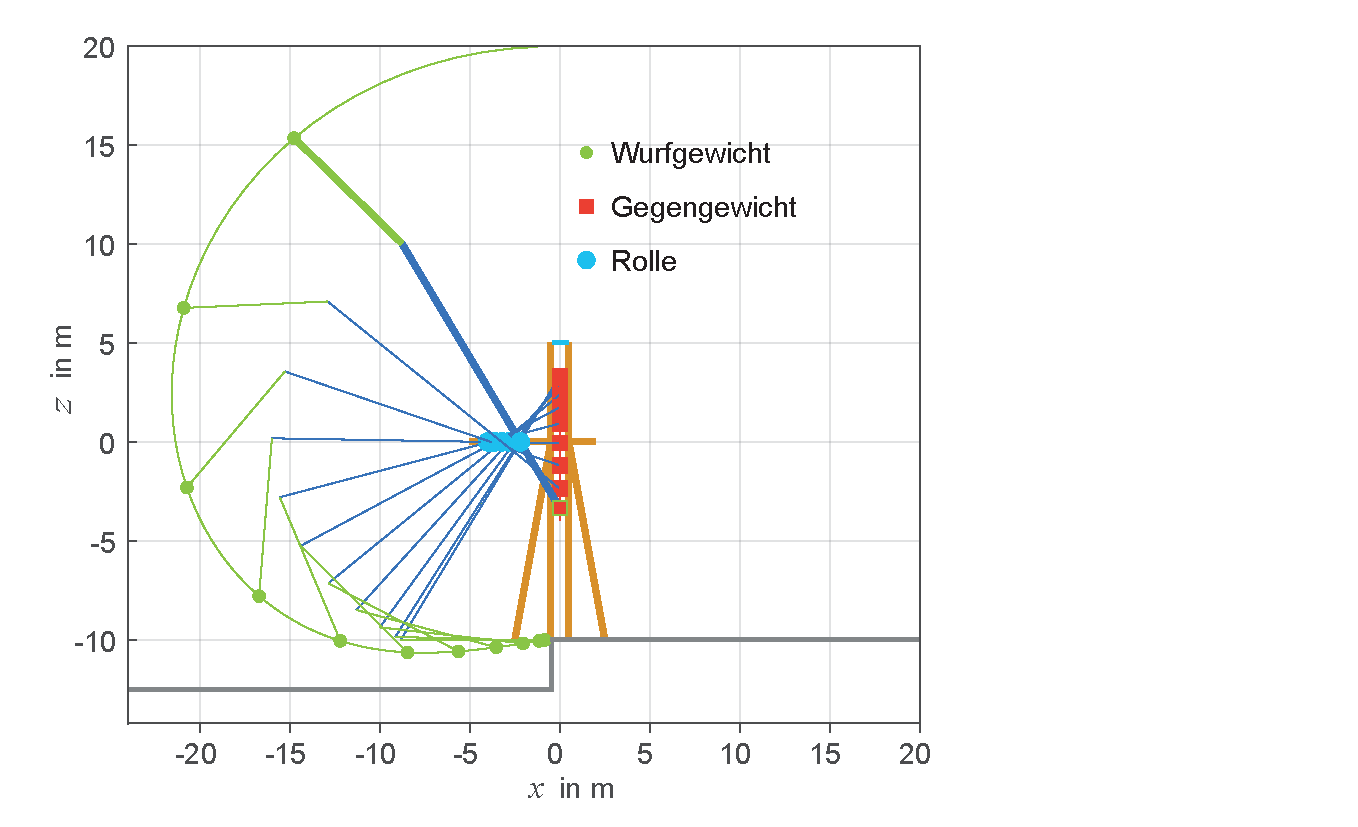
\includegraphics[width=\textwidth]{FloatingArmSim.pdf}
		\caption[Bewegungsabl�ufe und Reichweitenberechnung Floating Arm Trebuchet.]{Bewegungsabl�ufe und Reichweitenberechnung beim \textit{Floating Arm Trebuchet}, \vgl \mlbewref{TrebuchetSim01.m}}\label{abb:bew_FloatArm02}
		\end{figure}

		Wir wollen zun�chst annehmen, dass es keine weiteren zu ber�cksichtigenden Zwangsbedingung gibt (au�er der bereits verarbeiteten $z_\text{G}=0$).
		Das bedeutet insbesondere, dass die H�he $h$ gro� genug ist, um das Wurfgeschoss jederzeit als frei h�ngend zu betrachten. 
		Wir brauchen deshalb die Schleifphase auf dem Boden zun�chst nicht zu ber�cksichtigen.
		\begin{align}
			\mathcal{L} & = \frac{m_\text{W}}{2} \lek \lk \dot{\delta}\,l_\text{S}\,\sin(\delta) -\dot{\gamma}\,\sin(\gamma)\,(B + b) \rk^2 + \lk b\,\dot{\gamma}\,\cos(\gamma) - \dot{\delta}\,l_\text{S}\,\cos(\delta) \rk^2 \rek \nonumber \\
		& + \frac{m_\text{B}}{2} \lek B^2\,\,\dot{\gamma}^2\,\cos(\gamma)^2 \rek \nonumber + \frac{J_\text{T}}{2}\,\dot{\gamma}^2 \\
		& + g \, m_\text{W}\, b\,\sin(\gamma) - g \, m_\text{W}\,l_\text{S}\,\sin(\delta) - B\,m_\text{G}\,g\,\sin(\gamma) + \frac{m_\text{T}}{2}\,g\,(b-B)\,.
		\end{align}
                Die Lagrange-Gleichungen berechnen wir mit Hilfe der \textit{Symbolic Math Toolbox} in \mlbewref{TrebuchetLGL01.m}. 
		Die Bewegungsabl�ufe sind f�r zwei Parameters�tze in der \figref{bew_FloatArm02} dargestellt. 
		Die Wurfweiten sind beeindruckend und in Tabelle \ref{tab:bew_trebuchet_02} gelistet. 
		Sie sind deutlich gr��er als beim \anf{regul�ren} Trebuchet (Warum?).\\
		Man beachte, dass die H�he der Rolle (Drehpunkt) zu allen Zeiten �ber dem Graben im Boden des Trebuchet sein muss, \dh der Betrag der H�he $h$ muss mindestens $\abs{h} = b \sin\gamma - l_\text{S}\sin\delta$ sein.

	\subprob{Mit Zwangsbedingung (mit Schleifphase am Anfang)}

Die Situation f�hrt wieder auf ein sogenanntes \emph{Differential-Algebraisches (DAE) System}\index{Differential-Algebraisches System}.
Wir sind einem solchen bereits in Kap. \ref{kap:bew_trebuchet} beim Trebuchet (Modell 4) in der Gleichung \eqref{eq:bew_treb17a} begegnet.
Die L�sung dieses DAE-Systems erfolgt auch hier mit der \odeefs-Routine von \matlab{} (siehe \kap{bew_matlab_dgl} und \mscr{} \mlbewref{TrebSimDAE.m}).
Wir �berlassen das dem Leser als zus�tzliche �bung.

\end{subprobs}

Wer das Trebuchet nicht nur auf dem Computer sondern auch physisch untersuchen m�chte, dem sei der Baukasten Trebuchet vom \textit{moses Verlag}, Kempen (Deutschland) empfohlen (\figref{bew_TrebuchetBausatz}), siehe auch die \onlineZ. \\

\begin{figure}[H]\centering
\centering
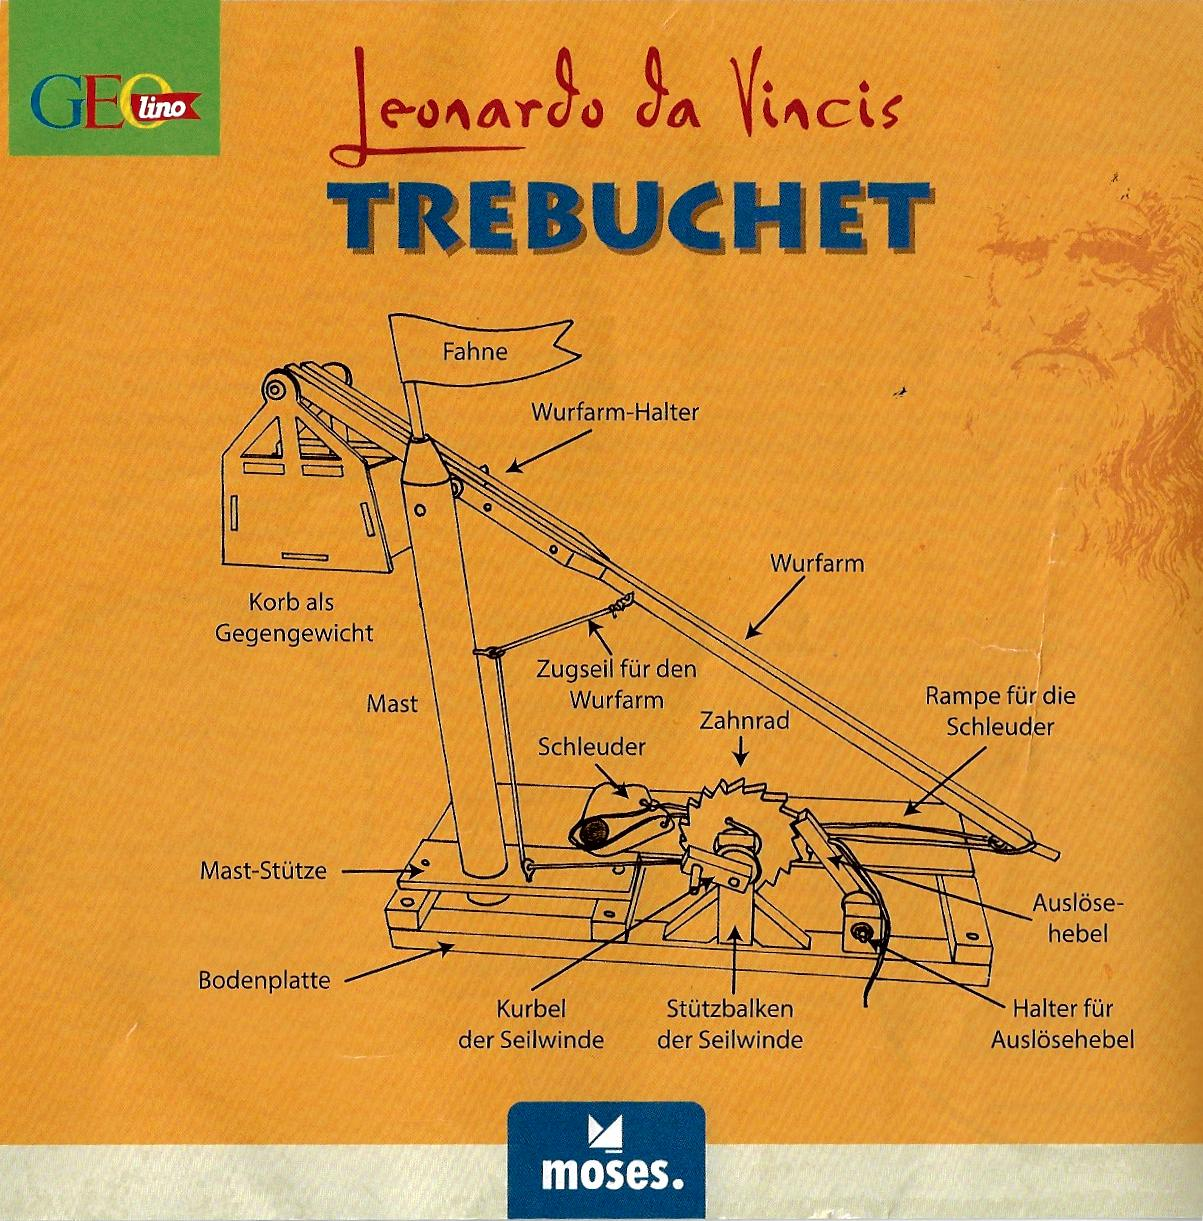
\includegraphics[width=0.4\textwidth]{Trebuchet02.jpg}
\caption[Bausatz eines Trebuchet]{Bausatz eines Trebuchet (\textit{moses. Verlag} Kempen, Deutschland)} 
\label{abb:bew_TrebuchetBausatz}
\end{figure}

\end{sol} 
%\href{PhysikUncut_Part1.pdf#prb:bew_Trebuchet}{\textcolor{blue} {$\rightarrow$ zur \probref{bew_Trebuchet}.}}\\      
\textcolor{blue} {$\rightarrow$ zur} \probref{bew_Trebuchet}.\\
\noindent\rule[1ex]{\textwidth}{0.5pt}  \newpage

%-----------------------------------------------------------------------------------------------------------
\hypertarget{lsg:bew_Trebuchet_II}{}
\begin{sol}{prob:bew_Trebuchet_II}\label{lsg:bew_Trebuchet_II} %�bung66
\textbf{Steinschleuder (\textit{Floating Arm Trebuchet} \uproman{2})} \\ \\
Die Lagrange-Funktion lautet:
        \begin{align*}
            \mathcal{L} = \frac{1}{2}\,m_\text{G}\,{\dot{z}_\text{G}{}}^2+\frac{1}{2}\,J_\text{B}\,{\dot{\gamma}}^2+\frac{1}{2}\,m_\text{W}\,\lk {\dot{x}_\text{W}{}}^2+{\dot{z}_\text{W}{}}^2\rk-m_\text{G}\,g\,z_\text{G}-m_\text{W}\,g\,z_\text{W}\,.
        \end{align*}
Wir schreiben die Massen der beteiligten Komponenten als Matrix $\mathbb{M}$:
        \begin{align*}
        \mathbb{M}=
            \begin{pmatrix}
            m_\text{G} & 0 & 0&0&0\\
            0&J_\text{B}&0&0&0\\
            0&0&m_\text{W}&0&0 \\
            0&0&0&m_\text{W}&0 \\
            0&0&0&0&0
            \end{pmatrix}\,.
        \end{align*}
Die Vektoren f�r die generalisierten Koordinaten $\vec{q}$, deren Beschleunigung $\ddot{\vec{q}}$, sowie die wirkenden Kr�fte lauten:
\begin{equation*}
    \vec{q} = 
	    \begin{pmatrix}
	    z_\text{G}\\
	    \gamma\\
	    x_\text{W} \\
	    z_\text{W} \\
	    \delta
	    \end{pmatrix}, \qquad
    \ddot{\vec{q}} = 
	    \begin{pmatrix}
	    \ddot{z}_\text{G}\\
	    \ddot{\gamma}\\
	    \ddot{x}_\text{W} \\
	    \ddot{z}_\text{W} \\
	    \ddot{\delta}
	    \end{pmatrix}
	\qquad \text{und} \qquad
    \vec{F} = 
		\begin{pmatrix}
		-m_\text{G}\,g\\
		0\\
		0 \\
		-m_\text{W}\,g \\
		0
		\end{pmatrix}\,.
\end{equation*}
Wir m�ssen nun jeweils f�r die einzelnen Phasen der Bewegung den jeweiligen Vektor der Zwangsbedingungen $\vec{f}$ bestimmen, daraus die Jacobi-Matrix $\d \vec{f}/\d \vec{q}$ und den zugeh�rigen Kraftvektor $\vec{F}_\text{R}$, um die Matrix-Gleichung f�r die \odeefs-Routine 
        \begin{align*}
            \begin{bmatrix}
            \mathbb{M} & \frac{\d \vec{f}}{\d \vec{q}} \\
             \lk\frac{{\d \vec{f}}}{\d \vec{q}}\rk^T& 0
            \end{bmatrix}
            \begin{pmatrix}
            \ddot{\vec{q}}\\
            \vec{\lambda}
            \end{pmatrix}
            =
            \begin{pmatrix}
            \vec{F}\\
            \vec{F}_\lambda
            \end{pmatrix}
        \end{align*}
aufzuschreiben (siehe \eqref{eq:bew_treb17b}). 
F�r die Berechnung k�nnen wir von der Symbolic Tool Box von \matlab{} Gebrauch machen.

�berlegen wir uns zuerst die Zwangsbedingungen.
In den verschiedenen Phasen der Bewegung k�nnen folgende Einschr�nkungen gelten:
    \begin{enumerate}
        \item [A)] Der bewegliche Arm $b$ ruht auf dem linken Rollrad des Querarms der L�nge $L_\text{Q}$ in einer Gelenkverbindung.
          Damit muss gelten
            \begin{align*}
                f_\text{A} = L_\text{Q}\,\sin\gamma+\lk H-z_\text{G}\rk\,\cos\gamma = 0\,.
            \end{align*}
        \item [B)] Ab etwa der Mitte der Abw�rtsbewegung kommt der bewegliche Arm (und damit auch das Rollrad) in die zweite Gelenkverbindung, sodass dann gilt
            \begin{align*}
                f_\text{B} = z_\text{G} - l_\text{Q}\,\sin\gamma-H\,.
            \end{align*}
        \item [C)] Das Wurfgewicht in der Schleuder bewegt sich anfangs auf der Rampe, welche mit Winkel $\beta$ aufgestellt ist, also
             \begin{align*}
                f_\text{C} = x_\text{W}\,\sin\alpha+ z_\text{W}\,\cos\alpha = 0\,.
            \end{align*}
        \item [D)] Das Wurfgewicht h�ngt am Schleuderseil der L�nge $l_\text{S}$.
          Hier kommt die f�nfte generalisierte Variable $\delta$ ins Spiel, f�r die es interessanterweise keine eigene Bewegungsgleichung gibt.
          Es gilt
            \begin{align*}
            {f_\text{D}}_{1,2} = 
            \left\{
            \begin{aligned}
        	 -b\,\cos\gamma-x_\text{W}+l_\text{S}\,\cos\delta \\
	        z_\text{G}-b\,\sin\gamma-z_\text{W}+ l_\text{S}\,\sin\delta
            \end{aligned}
            \right\} = 0\,.
            \end{align*}
            Man beachte, dass $f_D$ eine Vektorbedingung darstellt, $b$ ist die L�nge des Arms.
    \end{enumerate}
Wir betrachten nun die einzelnen Phasen.        
\textbf{\textit{Phase 1:}} Abw�rtsbewegung von $\gamma_0$ bis $\gamma = 0$ (Mitte der Bewegung) Schleuder auf der Rampe.\\ 
Der Vektor der Zwangsbedingung lautet:
        \begin{align*}
        \vec{f}_1 =
            \begin{Bmatrix}
            {f_\text{D}}_1\\
            {f_\text{D}}_2 \\
            {f_\text{A}} \\
            {f_\text{C}}
            \end{Bmatrix}\,.
        \end{align*}
Damit lautet die Jacobi-Matrix   
    \begin{align*}
    \frac{\d \vec{f}_1}{\d \vec{q}}= 
        \begin{bmatrix}
        0  & +b\,\sin\gamma & -1 & 0 & -l_\text{S}\,\sin\delta\\ 
        1  & -b\,\cos\gamma & 0 & -1 & +l_\text{S}\,\cos\delta \\
        -\cos\gamma ~~~&~L_\text{Q}\,\cos\gamma - \lk H-z_\text{G}\rk\sin\gamma ~~~& 0 &0&0 \\
        0 & 0 &\sin\alpha ~~~& \cos\alpha ~~~& 0
        \end{bmatrix}
    \end{align*}
und der resultierende Beschleunigungsvektor
    \begin{align*}
        {\vec{a}_1}_\lambda = 
        \begin{pmatrix}
        -b\,\dot{\gamma}^2\,\cos\gamma+l_\text{S}\,\dot{\delta}^2\,\cos\delta\\
        -b\,\dot{\gamma}^2\,\sin\gamma+l_\text{S}\,\dot{\delta}^2\,\sin\delta\\
        -2\dot{z}_\text{G}\,\dot{\gamma}\,\sin\gamma + \dot{\gamma}^2\,\lek L_\text{Q}\,\sin\gamma+\lk H-z_\text{G}\rk \cos\gamma \rek\\
        0
        \end{pmatrix}\,.
    \end{align*}
        
\textbf{\textit{Phase 2:}} Der bewegliche Balken kommt in die Quertr�ger-Gelenkaufnahme, die Schleuder ist noch auf der Rampe.\\
Die geltenden Zwangsbedingungen sind
        \begin{align*}
        \vec{f}_2 =
            \begin{Bmatrix}
            {f_\text{D}}_1\\
            {f_\text{D}}_2 \\
            {f_\text{B}}\\
            {f_\text{C}}
            \end{Bmatrix}\,,
        \end{align*} 
       wodurch sich die Jacobi-Matrix   
        \begin{align*}
        \frac{\d \vec{f}_2}{\d \vec{q}}= 
            \begin{bmatrix}
            0 ~~& +b\,\sin\gamma ~~~&-1 & 0 & -l_\text{S}\,\sin\delta \\
            1 ~~& -b\,\cos\gamma ~~~& 0 &-1 & +l_\text{S}\,\cos\delta \\
            1 ~~& -l_\text{Q}\,\cos\gamma ~~~&0&0&0 \\
            0 ~~&0&\sin\gamma~~~&\cos\gamma~~~&0
            \end{bmatrix}
        \end{align*}
        und die folgende Beschleunigung ergibt:
        \begin{align*}
            {\vec{a}_2}_\lambda = 
            \begin{pmatrix}
            -b\,\dot{\gamma}^2\,\cos\gamma + l_\text{S}\,\dot{\delta}^2\,\cos\delta\\
            -b\,\dot{\gamma}^2\,\sin\gamma + l_\text{S}\,\dot{\delta}^2\,\sin\delta\\
           -l_\text{Q}\,\dot{\gamma}^2\,\sin\gamma\\
            0
            \end{pmatrix}\,.
        \end{align*}
        
\textbf{\textit{Phase 3a:}} Der beweglicher Balken ist in der Quertr�ger-Gelenkaufnahme gelagert, aber die Schleuder hat sich von der Rampe gel�st.
Es gelten also nun nur noch folgende Zwangsbedingungen:
        \begin{align*}
        \vec{f}_\text{3a} =
            \begin{Bmatrix}
            {f_\text{D}}_1\\
            {f_\text{D}}_2 \\
            {f_\text{B}}
            \end{Bmatrix}.
        \end{align*}    
       Die Jacobi-Matrix hat entsprechend auch eine Dimension weniger als zuvor und lautet
        \begin{align*}
        \frac{\d \vec{f}_\text{3a}}{\d \vec{q}}= 
            \begin{bmatrix}
            0 ~~& +b\,\sin\gamma ~~&-1 ~&0 & -l_\text{S}\,\sin\delta \\
            1 ~~& -b\,\cos\gamma & 0 &-1 ~~& +l_\text{S}\,\cos\delta \\
            1 ~~& -l_\text{Q}\,\cos\gamma ~~~&0&0&0 \\
            \end{bmatrix}\,,
        \end{align*}
        woraus sich als Beschleunigung ergibt:
        \begin{align*}
            {\vec{a}_\text{3a}}_\lambda = 
            \begin{pmatrix}
            -b\,\dot{\gamma}^2\,\cos\gamma+l_\text{S}\,\dot{\delta}^2\,\cos\delta\\
            -b\,\dot{\gamma}^2\,\sin\gamma+l_\text{S}\,\dot{\delta}^2\,\sin\delta\\
           -l_\text{Q}\,\dot{\gamma}^2\,\sin\gamma
            \end{pmatrix}\,.
        \end{align*}
        
\textbf{\textit{Phase 3b:}} Der bewegliche Arm ist im linken Gelenk, die Schleuder ist nicht mehr auf der Rampe.\\
Dieser Fall tritt zwar nur mit geringer Wahrscheinlichkeit auf, aber dennoch -- seine Zwangsbedingungen sind:
        \begin{align*}
        \vec{f}_\text{3b} =
            \begin{Bmatrix}
            {f_\text{D}}_1\\
            {f_\text{D}}_2 \\
            {f_\text{A}}
            \end{Bmatrix}.
        \end{align*}   
    Also Jacobi-Matrix ergibt sich 
        \begin{align*}
        \frac{\d \vec{f}_\text{3b}}{\d \vec{q}}= 
            \begin{bmatrix}
            0 ~~& b\,\sin\gamma ~~&-1~~&0 ~~& -l_\text{S}\,\sin\delta \\
            1 & -b\,\cos\gamma & 0 &-1 ~& +l_\text{S}\,\cos\delta \\
            -\cos\gamma ~~& L_\text{Q}\,\cos\gamma-\lk H-z_\text{G}\rk\,\sin\gamma~~~ &0~&0&0 \\
            \end{bmatrix}\,,
        \end{align*}
        und f�r die Beschleunigung folgt
        \begin{align*}
            {\vec{a}_\text{3b}}_\lambda = 
            \begin{pmatrix}
            -b\,\dot{\gamma}^2\,\cos\gamma+l_\text{S}\,\dot{\delta}^2\,\cos\delta\\
            -b\,\dot{\gamma}^2\,\sin\gamma+l_\text{S}\,\dot{\delta}^2\,\sin\delta\\
           -2\dot{z}_\text{G}\,\dot{\gamma}\,\sin\gamma+\dot{\gamma}^2\lek L_\text{Q}\,\sin\gamma+\lk H-z_\text{G}\rk \,\cos\gamma\rek
            \end{pmatrix}\,.
        \end{align*} 
        \medskip
      
Bei der Berechnung der zeitlichen Entwicklung beginnt man entsprechend der Anfangsbedingungen mit einem bestimmten $\vec{f}_r$ und sucht dann nach den verschwindenden Eigenwerten $\lambda_r$, bzw. nach deren Vorzeichenwechsel.
F�r bestimmte Zeitschritte werden also die Koordinaten $q_\text{i}$ und die dazugeh�rigen Eigenwerte $\lambda_\text{r}$ explizit berechnet. 
Solange, bis einer der Eigenwerte das Vorzeichen wechselt. 
Von dort aus muss erneut �berlegt werden, welche Zwangsbedingungen gelten und wie der entsprechende Vektor der Zwangsbedingungen aussehen muss. 
Die Rechnung muss dann erneut ausgef�hrt werden, nat�rlich mit aktualisierten Zwangsbedingungsvektor $\vec{f}_r$ und der entsprechend neuen Beschleunigung $\vec{a}_r$, solange bis die Abwurf-Bedingung erf�llt ist.\\
Die Umsetzung in ein \matlab{}-Skript �berlassen wir dem Leser als zus�tzliche �bung.
   
\end{sol} 
%\href{PhysikUncut_Part1.pdf#prb:bew_Trebuchet_II}{\textcolor{blue} {$\rightarrow$ zur \probref{bew_Trebuchet_II}.}}\\      
\textcolor{blue} {$\rightarrow$ zur} \probref{bew_Trebuchet_II}.\\
\noindent\rule[1ex]{\textwidth}{0.5pt}  \newpage


%-----------------------------------------------------------------------------------------------------------
\hypertarget{lsg:bew_Murphy}{}
\begin{sol}{prob:bew_Murphy}\label{lsg:bew_Murphy} %�bung67
\textbf{Murphy's Law} \\ \\

\begin{figure}[H]\centering
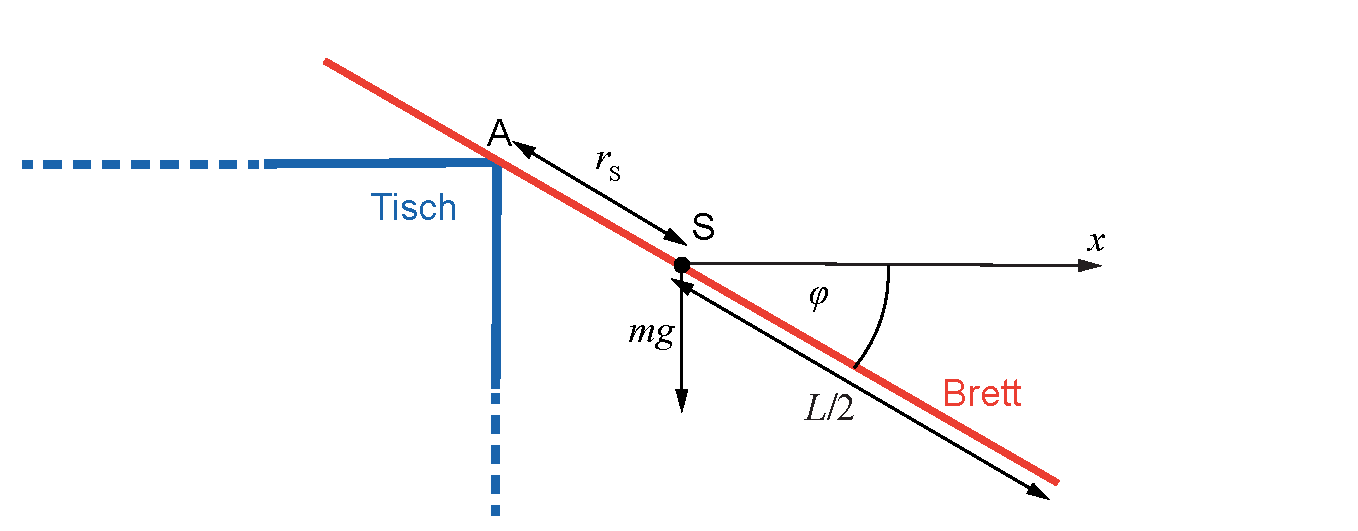
\includegraphics[width=\textwidth]{MurphysLaw.pdf}
\caption[Modellversuch zu Murphy's Law]{Modellversuch zu Murphy's Law. (Parameter siehe Text.)} 
\label{abb:bew_toast01}
\end{figure}

Diese nicht ganz so ernst gemeinte �bungsaufgabe ist bereits verschiedentlich in der Literatur  behandelt. Wir verweisen dazu auf die Referenzen \cite{Matthews1995, Mahajan2022}. Wir betrachten die Brotscheibe auf einem Tisch der H�he $H$ als ein d�nnes Brett der L�nge $L_\text{B}$ und der Masse $m$ (\figref{bew_toast01}), dessen Tr�gheitsmoment $J_\text{s}$ (bezogen auf den Schwerpunkt $S$) bekannt sei. Der Abstand des Schwerpunktes von der Tischkante sei $r_\text{S}$ und $\varphi$ sei der Winkel, den das Brett zur Horizontalen bildet. Die Lagrange-Funktion ist dann gegeben durch: 
\begin{align*}
    \mathcal{L} = \frac{1}{2}\,m\lek \dot{r}_\text{S} +  \lk r_\text{S}{}^2 + \frac{J_\text{S}}{m}\rk\,\dot{\varphi}^2\rek + m\,g\,r_\text{S}\,\sin\varphi\,,
\end{align*}
wobei wir f�r das Tr�gheitsmoment des Stabes um den Drehpunkt A den Steinerschen Satz benutzt haben. Die beiden verallgemeinerten Koordinaten sind die Schwerpunktabstandskoordinate $r_\text{s}$ und der Drehwinkel $\varphi$. \\
Die Lagrange-Gleichungen ergeben dann folgendes nichtlineares gekoppeltes DGL-System:
\begin{subequations}
\begin{align}
    \ddot{r}_\text{S} &= r_\text{S}\,\dot{\varphi}^2 + g\,\sin\varphi \,, \label{eq:bew_toast01a}\\
    \ddot{\varphi} &= \frac{r_\text{S}\,\lk g\,\cos\varphi - 2\,\dot{r}_\text{S}\,\dot{\varphi} \rk}{r_\text{S}{}^2 + J_\text{S}/m} \,,  \label{eq:bew_toast01b}
\end{align} 
\end{subequations}
f�r dessen Herleitung wir das \mscr~\mlbewref{MurphysLaw.m} benutzt haben.
Dieses DGL-System gilt so lange das Brett Kontakt zum Tisch hat, danach f�hrt das Brett eine freie Rotation (\vgl Kapitel \ref{kap:bew_kfKreisel}) aus.
Man m�sste f�r den Kontakt in der Anfangsphase eigentlich eine Zwangsbedingung einf�hren und w�rde dann mit einem entsprechenden Lagrange-Multiplikator ein DAE-System, \vgl Kap. \ref{kap:bew_trebuchet} \bzw die \onlineZ (\matlab Anhang) erhalten.
Dieses System l�st man dann bis die Zwangsbedingung verletzt ist.\\
Man kann hier aber einen etwas einfacheren Weg w�hlen, da bei Betrachtung von \figref{bew_toast01} klar wird, dass beim Abrutschen des Bretts eine Rotation desselben nur durch die von der Kante (Punkt A) ausgef�hrte Normalkraft $F_\text{N}$ (\bzw durch das daraus resultierende Drehmoment $M= F_\text{N}\,r_\text{S})$ erfolgen kann.
Verschwindet also die Normalkraft, so wird auch die Winkelbeschleunigung $\ddot{\varphi} = 0$.\\
Dann folgt aus \eqref{eq:bew_toast01b} f�r diesen Zeitpunkt $t_\text{F}$:
\begin{align}
    g\,\cos\varphi_\text{F} = 2\,\dot{r}_\text{S,F}\, \,\dot{\varphi}_\text{F}\,. \label{eq:bew_toast02}
\end{align}
Wir m�ssen also das DGL-System f�r $\varphi,r_\text{S}$ bis zum Zeitpunkt $t_\text{F}$ l�sen , bei dem \eqref{eq:bew_toast02} erf�llt ist.
Danach rotiert das Brett mit konstanter Winkelgeschwindigkeit $\dot{\varphi}_\text{F}$ bis eines seiner Enden den Boden ber�hrt.
Die Simulation ist f�r verschiedene Tischh�hen $H$ und der L�nge $L_\text{B}$ als Parameter in \cite{Mahajan2022} beschrieben und in \mlbewref{MurphysLaw.m} ausgef�hrt.\\
Das wesentliche Ergebnis dieser Simulation (\figref{bew_toast02}) ist, dass bei einer Tischh�he von ca. $ \SI{75}{\centi\metre}$ in der Tat das Butterbrot auf der Butterseite landen w�rde (und zwar abh�ngig von der m�glicherweise randomisierten Anfangsbedingung deterministisch), w�hrend bei einer Tischh�he von $\SI{2.1}{\metre}$ (\zb in Gullivers Land der Riesen) genau der umgekehrte Effekt auftreten w�rde. Es ist also Newton und nicht Murphy f�r diesen speziellen Fall verantwortlich zu machen! \\
Wir m�chten noch erw�hnen, dass der Autor von \cite{Matthews1995} im Jahre 1996 den Ig-Nobelpreis in Physik f�r eben diese Ver�ffentlichung erhielt. Dabei sei darauf hingewiesen, dass er mit Unterst�tzung von ca. $\SI{1000}{}$ Sch�lern in mehr als $\SI{21000}{}$ Butterbrot-Fallversuchen nachweisen konnte, dass $\SI{62}{\percent}$ auf der Butterseite landeten. Wenn das keine eindrucksvolle Best�tigung dieser Theorie ist. 
\begin{figure}[H]
\centering
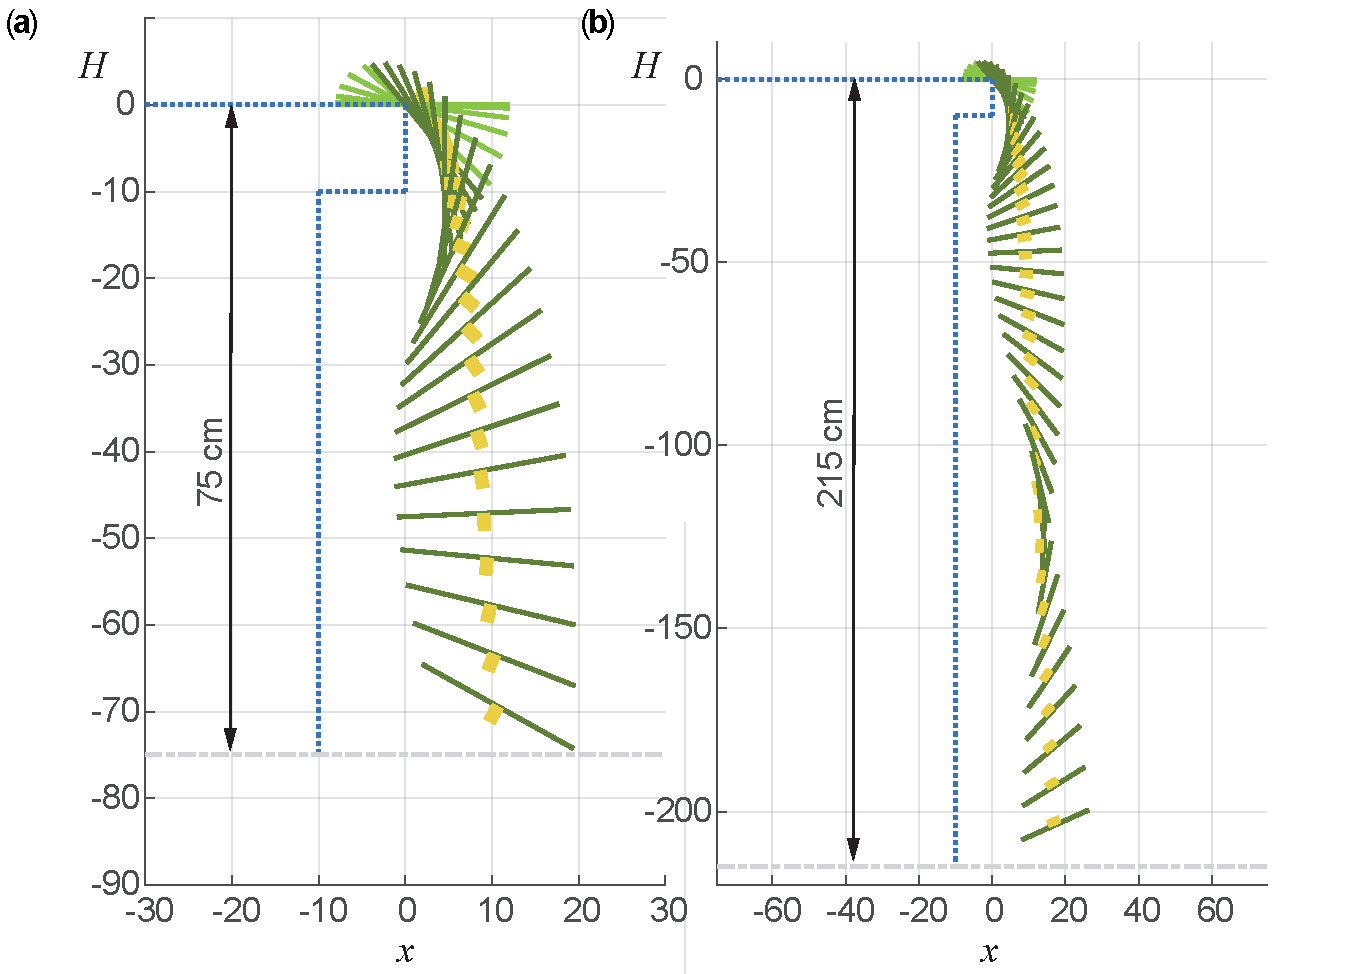
\includegraphics[width=\textwidth]{MurphysLaw2.pdf}
\caption[Computersimulation zu Murphy's Law]{Computersimulation zu Murphy's Law. Fallversuch eines Butterbrotes der L�nge 20 cm \fa Tischh�he $ \SI{75}{\centi\metre}$, \fb $ \SI{210}{\centi\metre}$. Man beachte die unterschiedlichen Ma�st�be der Abbildungen. Die gelben Balken zeigen die "`Butterseite"' an, die hellgr�ne Balken, die Phase des Abkippens (Brot/Brett ist noch im Kontakt mit dem Tisch),  dunkelgr�n die Phase der freien Rotation. )} 
\label{abb:bew_toast02}
\end{figure}
\end{sol}
%\href{PhysikUncut_Part1.pdf#prb:bew_Murphy}{\textcolor{blue} {$\rightarrow$ zur \probref{bew_Murphy}.}}\\      
\textcolor{blue} {$\rightarrow$ zur} \probref{bew_Murphy}.\\
\noindent\rule[1ex]{\textwidth}{0.5pt}  \newpage



%-----------------------------------------------------------------------------------------------------------

%\hypertarget{lsg:bew_relLorentzkraft}{}
%\begin{sol}{prob:bew_relLorentzkraft}\label{lsg:bew_relLorentzkraft}
%\textbf{Lagrange-Funktion f�r relativistisches und nicht-relativistisches Teilchen unter Einflu� einer Lorentz-Kraft} \\ \\
%
    %Wir wollen zeigen, dass aus der Lagrange-Funktion \eqref{eq:bew_rel09} f�r $v \ll c$ die Bewegungsgleichung mit der bekannten Lorentz-Kraft herauskommt. \\
    %Wir nehmen an, dass ein homogenes $\vec{E}$-Feld in $x$-Richtung wirkt. In diesem Fall ist 
            %\begin{align}
                %\vec{E} = E\,\hat{x}
            %\end{align}
    %und eine sinnvolle Wahl der Potentiale ist $\phi = -E\,x$ und $\vec{A}=0$. \\
    %Dann ist $\vec{E} = -\vec{\nabla}\,\phi = E\,\vec{x}$. Es folgt $A_0 = -E\,x \equiv -E\,x^1$, $A_1 =A_2=A_3 = 0$ und die Bewegungsgleichungen lauten, f�r $u_0$:
            %\begin{align}
                %m\,\frac{\D u_0}{\D \tau} = -\frac{q}{c}\,\frac{\D A_0}{\D \tau} + \frac{q}{c}\,u^0\,\frac{\d A_0}{\d x^0 } = \frac{q\,E}{c}\,\frac{\D x^1}{\D \tau}- \killA{\frac{q\,E}{c}\,u^0\,\underbrace{\frac{\d x^1}{\d x^0}}_{\substack{=0}}}\,.
            %\end{align}
    %Es folgt
            %\begin{align}
                %\frac{\D u^0}{\D \tau} = \frac{\D u_0}{\D \tau} = \frac{q\,E}{m\,c}\,\frac{\D x^1}{\D \tau} = \frac{q\,E}{m\,c}\,u^1\,.
            %\end{align}
    %Und f�r $u_1$:
            %\begin{align}
                %m\,\frac{\D u_1}{\D \tau} = \killA{-\frac{q}{c}\,\frac{\D A_1}{\D \tau}} + \frac{q}{c}\,u^0\,\frac{\d A_0}{\d x^1} = -\frac{q}{c}\,u^0\,E = -\frac{q\,E}{c}\,u^0\,.
            %\end{align}
    %Es folgt
        %\begin{align}
            %\frac{\D u^1}{\D \tau} = -\frac{\D u_1}{\D \tau}= +\frac{q\,E}{m\,c}\,u^0\,.
        %\end{align}
%Wir erhalten also zwei gekoppelte Differentialgleichungen f�r $u^0$ und $u^1$. Wenn wir jeweils eine in die andere einsetzen, erhalten wir
        %\begin{align}
            %\frac{\D^2\,u^0}{\D \tau^2} &= \frac{q\,E}{m\,c}\,\frac{\D\,u^1}{\D \tau} = \lk \frac{q\,E}{m\,c}\rk^2\,u^0 \,,\\
            %\frac{\D^2\,u^1}{\D \tau^2} &= \frac{q\,E}{m\,c}\,\frac{\D\,u^0}{\D \tau} = \lk \frac{q\,E}{m\,c}\rk^2\,u^1 \,.
        %\end{align}
%Wir betrachten speziell die Anfangsbedingung $v\lk 0\rk = 0\rightarrow u^0\lk 0\rk = c$, $u^1\lk 0\rk = u^2\lk 0\rk = u^3\lk 0\rk = 0$ (\glqq Teilchen in Ruhe\grqq{}). Dann ist die L�sung 
        %\begin{align}
            %u^0\lk \tau\rk &= c\,\cosh\,\frac{q\,E}{m\,c}\,\tau\,, \\
            %u^1\lk \tau\rk &= c\,\cosh\,\frac{q\,E}{m\,c}\,\tau\,,
        %\end{align}
%(Als Probe nachrechnen, dass wir
        %\begin{align}
            %u_\mu\,u^\mu = \lk u^0\rk^2 - \lk u^1\rk^2 = c^2\,\lk \cosh^2\,\frac{q\,E}{m\,c}\,\tau -\sinh^2\,\frac{q\,E}{m\,c}\,\tau\rk = c^2
        %\end{align}
%erhalten, so wie es sein muss.)\\
%Weiter folgt f�r die zus�tzlichen Anfangsbedingungen $x^\mu\lk 0\rk = 0$:
        %\begin{align}
            %c\,t = x^0\lk \tau\rk  &= \int\limits_0^\tau \D \tau'\,u^0\lk\tau'\rk = \frac{m\,c^2}{q\,E}\,\sinh\,\frac{q\,E}{m\,c}\,\tau\,, \\
            %x= x^1\lk\tau\rk &= \int\limits_0^\tau \D \tau'\,u^1\lk\tau'\rk = \frac{m\,c^2}{q\,E}\,\lk\cosh\,\frac{q\,E}{m\,c}\,\tau -1\rk \nonumber \\
            %&= \frac{m\,c^2}{q\,E}\lk \sqrt{\sinh^2\,\frac{q\,E}{m\,c}\,\tau+1}-1 \rk= \frac{m\,c^2}{q\,E}\,\lk\sqrt{\lk\frac{q\,E}{m\,c}\,t\rk^2+1}-1\rk\,.
        %\end{align}
%F�r kleine Zeiten ist dies
        %\begin{align}
            %x \cong \frac{m\,c^2}{q\,E}\,\lk \killA{1} + \frac{1}{2}\,\lk\frac{q\,E}{m\,c}\rk^2 t^2\killA{-1}\rk \frac{1}{2}\,\frac{q\,E}{m}\,t^2 \equiv \frac{1}{2}\,a\,t^2\,.
        %\end{align}
%Das ist genau die nicht-relativistische, gleichf�rmig beschleunigte Bewegung. Unsere Rechnung stimmt also im nicht-relativistischen Grenzfall mit der Newtonschen Mechanik �berein.\\
%F�r gro�e Zeiten folgt dagegen
        %\begin{align}
            %x \cong \frac{m\,c^2}{q\,E}\,\frac{q\,E}{m\,c}\,t =c\,t\,.
        %\end{align}
%Das Teilchen bewegt sich also f�r $t \gg \frac{m\,c}{q\,E}$ praktisch mit Lichtgeschwindigkeit. Es wird aber trotz des
%gleichf�rmigen beschleunigenden Feldes niemals schneller als $c$.
%
%\end{sol} 
%%\href{PhysikUncut_Part1.pdf#prb:bew_relLorentzkraft}{\textcolor{blue} {$\rightarrow$ zur \probref{bew_relLorentzkraft}.}}\\      
%\textcolor{blue} {$\rightarrow$ zur} \probref{bew_relLorentzkraft}.\\
%\noindent\rule[1ex]{\textwidth}{0.5pt}  \newpage
%




%%%%%%%%%%%%%%%%%%%%%%%%%%%%%%%%%%%%%%%%%%%%%%%%%%%%%%%%%%%%%%%%%%%%%%%%%%%%%%%%%%%%%%%%%%%%%%%%%%%%%%%%%%%%%%%%%%%%%%%%%%%%%%%%%%%%%%%%%%%





%\clearpage
%\section {L�sungsbeispiele \autoref{chap:hm} -- Himmelsmechanik}\label{chap:hm_lsguebungen}

Die in den L�sungsvorschl�gen angegebenen \mscre finden sich im GitHub unter \githubSN \bzw
in den \onlineZ{} (\MKc).\\
Sie sind wirklich als Vorschlag f�r eine m�gliche L�sung gedacht, wohl wissend, dass es in der Physik oft ganz verschiedene, manchmal auch elegantere als die hier vorgestellten L�sungen gibt, um ein Problem zu l�sen. Das macht ja gerade den Reiz der Physik aus.
Wir laden die Leser ein, ihre L�sungen auch unter \githubSN \bzw auf den online-Seiten (\MKc) zu teilen.
Wir sind in jedem Fall gespannt.
%%%-----------------------------------------------------------------------------------------------------------

\subsection{�bungen zu Raum und Zeit in der Himmelsmechanik}

\medskip

%-----------------------------------------------------------------------------------------------------------

\begin{sol}{prob:hm_trafo_koord}\label{lsg:hm_trafo_koord} %�bung1
\textbf{Transformation astronomischer Koordinatensysteme} \\
\begin{enumerate}[(a)]
	\item Wie im Kapitel \ref{kap:hm_koordinatensysteme} erl�utert, wird die Transformation von kartesischen Koordinaten aus einem KOS in ein anderes durch Rotationsmatrizen der Form $\mathbb{R}_{x,y,z}(\xi)$ mit dem Drehwinkel $\xi$ und/oder Translationsvektoren beschrieben.
          Man kann sich diese durch geometrische Betrachtungen einfach ableiten.
          Wir geben die Matrizen im Folgenden an und verweisen darauf, dass die R�cktransformation bei Rotationen durch eine Drehmatrix mit dem Winkel $-\xi$ beschrieben wird, die dann wegen der Unitarit�t auf die transponierte Drehmatrix $\lk \mathbb{R}_{x,y,z}(\xi) \rk^\text{T}$ f�hrt.
Wir beschreiben das Vorgehen beispielhaft f�r einige ausgew�hlten Transformationen (siehe auch Beispiel \ref{bsp:herleitung_gauss_vek}):
\begin{itemize}
	\item \emph{Bahn (BA) -- Heliozentrisch-ekliptikal (HE):}
	\begin{align*}
	\mathbb{R}_1 &= \mathbb{R}_z(-\omega) = \lk
	      \begin{matrix} +\cos \omega &\; -\sin \omega &\; 0 \\
	                     +\sin \omega &\; +\cos \omega &\; 0 \\
                          0         &\;     0        &\; 1 
				\end{matrix} \rk  ~~,\\ 
	\mathbb{R}_2 &= \mathbb{R}_x(-i) = \lk
	      \begin{matrix} 1       &\; 0           &\; 0 \\ 
				               0       &\; +\cos i     &\; -\sin i \\ 
											 0       &\; +\sin i     &\; +\cos i 
				\end{matrix} \rk  ~~,\\
	\mathbb{R}_3 &= \mathbb{R}_z(-\Omega) = \lk
	    \begin{matrix} 
	            +\cos \Omega &\; -\sin \Omega &\; 0 \\
	            +\sin \Omega &\; +\cos \Omega &\; 0 \\
                 0         &\;     0        &\; 1 
			 \end{matrix} \rk ~~. 
	\end{align*}
	Die Gesamttransformation wird dann auch mit einer Matrix $\mathbb{U}(-\omega,-i,-\Omega)\!=\! \mathbb{R}_3 \mathbb{R}_2\mathbb{R}_1$ beschrieben.
        Durch Multiplizieren von $\mathbb{U}$ mit dem kartesischen Ausgangsvektor erhalten wir dann die kartesischen heliozentrischen Koordinaten
	\begin{align*}
	r\lk\begin{matrix} \cos b \cos l\\ \cos b \sin l\\ \sin b \end{matrix} \rk = \mathbb{U} \cdot r \lk\begin{matrix} \cos u \\ \sin u \\ 0 \end{matrix} \rk ~~,
	\end{align*}
	aus denen wir dann heliozentrisch die ekliptikalen Parameter $b,l,r$ ableiten k�nnen.\\
	\item \emph{Geozentrisch-ekliptikal (GE)- Geozentrisch-�quatorial (GA):}
		\begin{align*}
	\mathbb{R}_1 &= \mathbb{R}_x(-\epsilon) = \lk
	      \begin{matrix} 1       &\; 0           &\; 0 \\ 
				               0       &\; +\cos \epsilon     &\; -\sin \epsilon \\ 
											 0       &\; +\sin \epsilon     &\; +\cos \epsilon
				\end{matrix} \rk ~~. 
	\end{align*}
	Hier besteht die Transformation nur aus einer Matrix $\mathbb{U}(-\epsilon)\!=\! \mathbb{R}_1$.
        Durch Multiplizieren von $\mathbb{U}$ mit dem kartesischen (GE) Ausgangsvektor erhalten wir dann die kartesischen �quatorialen Koordinaten
	\begin{align*}
	r\lk\begin{matrix} \cos \delta \cos \alpha\\ \cos \delta \sin \alpha\\ \sin \delta \end{matrix} \rk =\mathbb{U} \cdot r \lk \begin{matrix} \cos b \cos l \\ \cos b \sin l \\ \sin l \end{matrix} \rk ~~,
	\end{align*}
	aus denen wir dann die geozentrisch-�quatorialen Koordinaten $\alpha,\delta$ ableiten k�nnen.
\end{itemize}
	\item Wir empfehlen zum Nachvollziehen der Navigationsmethoden fr�herer Jahre die ausf�hrlichen Darstellungen in \cite{Smart1986} und \cite{Weyer2012}.
\end{enumerate}

Wir vergleichen jetzt noch die Bahnparameter der Himmelsmechanik mit den Euler Winkeln\index{Euler-Winkel}, die wir in der Theorie des starren K�rpers (Band I) eingef�hrt hatten.
\begin{table}[h!]
    \centering
    \begin{tabular}{ll}
        \centering Euler-Winkel & Bahnparameter\\
        & \\
         1. Drehung um $\vec{e}_z$-Achse mit Winkel $\varphi$ 
         & 
         1. Drehung um $\vec{e}_z$-Achse mit Winkel $\Omega$ \\
         ~~~~$\mathbb{R}_z\lk\varphi\rk = 
         \begin{pmatrix}
         \cos\varphi & \sin\varphi & 0\\
         -\sin\varphi & \cos\varphi & 0\\
         0 & 0 & 1
         \end{pmatrix}$
         &
          ~~~~$\mathbb{R}_z\lk\Omega\rk  = 
         \begin{pmatrix}
         \cos\Omega & \sin\Omega & 0\\
         -\Omega\varphi & \cos\Omega & 0\\
         0 & 0 & 1
         \end{pmatrix}$\\
         &\\
         2. Drehung um Knotenlinie $\vec{e}_x{}'$ mit Winkel $\vartheta$ &
         2. Drehung um Knotenlinie $\vec{e}_x{}'$ mit Winkel i \\
        ~~~~$\mathbb{R}_x{}'\lk\vartheta\rk = 
         \begin{pmatrix}
         1 & 0 & 0 \\
         0 & \cos\vartheta & \sin\vartheta \\
         0 & -\sin\vartheta & \cos\vartheta
         \end{pmatrix}$ &
         ~~~~$\mathbb{R}_x{}'\lk i\rk = 
         \begin{pmatrix}
         1 & 0 & 0 \\
         0 & \cos i & \sin i \\
         0 & -\sin i & \cos i
         \end{pmatrix}$ \\
         & \\
         3. Drehung um $\vec{e}_z{}''$ mit Winkel $\psi$ & 
         3. Drehung um $\vec{e}_z{}''$ mit Winkel $\omega$ \\
         ~~~~$\mathbb{R}_z{}''\lk\psi\rk = 
         \begin{pmatrix}
         \cos\psi & \sin\psi & 0 \\
         -\sin\psi & \cos\psi & 0 \\
         0 & 0 & 1
         \end{pmatrix}$ &
          ~~~~$\mathbb{R}_z{}''\lk\omega\rk = 
         \begin{pmatrix}
         \cos\omega & \sin\omega & 0 \\
         -\sin\omega& \cos\omega & 0 \\
         0 & 0 & 1
         \end{pmatrix}$ 
    \end{tabular}
\end{table}\\
Wir sehen also, dass die Bahnparameter $\Omega, i, \omega$ den Euler-Winkeln entsprechen.

\end{sol}
\textcolor{blue} {$\rightarrow$ zur} \probref{hm_trafo_koord}.\\
\noindent\rule[1ex]{\textwidth}{0.5pt} \newpage \newpage

%-----------------------------------------------------------------------------------------------------------

\begin{sol}{prob:hm_erdrotation}\label{lsg:hm_erdrotation} %�bung2
\textbf{Verlangsamung der Erdrotation} \\ \\
Wenn man in die Formel \eqref{eq:hm_ueb_verl_erdrot} die Werte
\begin{align*}
a_\text{trop}&=365.2421988 ~, \\
n_\text{Tage}&\approx (2000+135)\cdot 365.25 \approx 779702 \:\text{d}\  \text{bzw. genauer}\\
n_\text{Tage}&=\text{J}2000 - \text{J}(15.04.136 \;\text{v.Chr.})\approx 779691 \:\text{d}
\end{align*}
einsetzt, erh�lt man f�r $\Delta T_\text{rot}\!\approx\!3.7\:\text{h}.$
Das ist recht beachtlich!
Daraus w�rde, wenn man die Sonnenfinsternis nicht mit der Ephemeridenzeit, sondern der um $\Delta T_\text{rot}\!=\!-3.7\:\text{h}$ verschobenen UT berechnet, die Sonnenfinsternis um $\Delta \lambda\!\approx\!55.5\degree$ weiter westlich stattgefunden haben.
Sie wurde aber in Babylon beobachtet.
Wenn man daher den berechneten Wert von $\Delta T_\text{rot}$ in Sekunden ($13300 \:\text{s}$) in die \figref{hm_rotgeschw_sonnenfinsternis} eintr�gt, sieht man eine gute �bereinstimmung mit den beobachteten Daten (siehe auch \cite{Stephenson2016,Steele1997}) und die \href{https://eclipse.gsfc.nasa.gov/SEsearch/SEsearchmap.php?Ecl=-1350415}{NASA Eclipse Web Site}. \\
Man kann sich jetzt noch die Frage stellen, ob man f�r die Verlangsamung der Erdrotation, die im Wesentlichen mit der Gezeitenreibung (siehe \kap{hm_gezeitenreibung}) erkl�rt wird, eine einfache Absch�tzung findet.
Wir betrachten dazu das Erde-Mond-System und vernachl�ssigen den Einfluss der Sonne.
Ferner nehmen wir der Einfachheit halber eine Bahnebene f�r Mond und Erde an und vernachl�ssigen auch die Polneigung der Erde.
F�r dieses System gilt Drehimpulserhaltung, der Gesamtdrehimpuls setzt sich dabei wie folgt zusammen:
\begin{figure}[H]
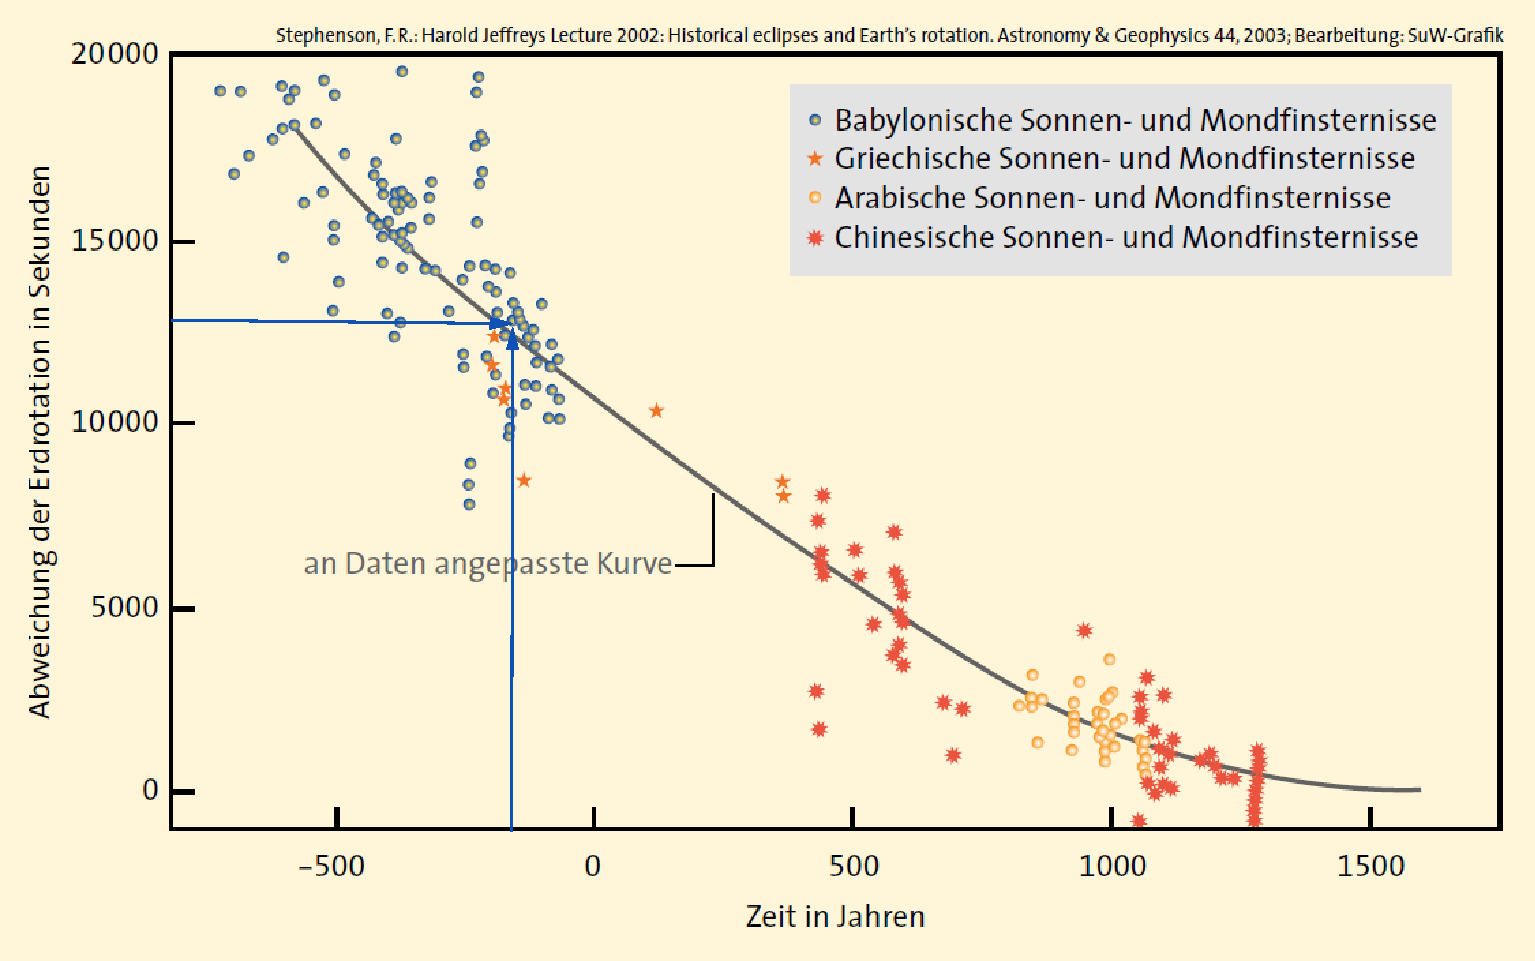
\includegraphics[width=\columnwidth]{SofiHistory.pdf}%
\caption[Abnahme der Rotationsgeschwindigkeit der Erde.]{Abnahme der Rotationsgeschwindigkeit der Erde aus Beobachtung von Sonnenfinsternissen \cite{Stephenson2016,Bastian2020}}%
\label{abb:hm_rotgeschw_sonnenfinsternis}% 
\end{figure}  
\begin{align*}
		\vec{L}_g =\sum \vec{L}_i = \vec{const} = \vec{L}_{\earth,\text{Rotation}} + \vec{L}_{\earth \text{/Mond},\text{Bahn}} + \vec{L}_\text{Mond, Rotation}  ~~.
\end{align*}
Die einzelnen Terme sind der Eigendrehimpuls der Erde, der Bahndrehimpuls des Mondes um die Erde und Eigendrehimpuls des Mondes, wobei wir letzteren auf Grund der Massenverh�ltnisse und der langsamen Rotation vernachl�ssigen k�nnen.
Eine Reduktion der Eigenrotations-Geschwindigkeit der Erde muss dann also zu einem Anwachsen des Bahndrehimpulses f�hren.
Da wir das Problem in einer Ebene behandeln wollen, k�nnen wir zu skalaren Gr��en �bergehen.
Der Betrag des Eigendrehimpulses der Erde ist dann gegeben durch $L_{\earth,\text{Rotation}} = J_{\earth} \omega_{\earth}$, der Bahndrehimpulsbetrag durch $L_{\earth \text{/Mond},\text{Bahn}} = m_{\text{M}} a_{\earth \text{M}} ^2 \omega_{\earth \text{M}}$.
Der Endzustand nach langer Zeit ($t \rightarrow \infty$) ist dann erreicht, wenn $ \omega_{\earth , \infty} = \omega_{\earth \text{M}, \infty}$, d.\,h. die Erde rotiert dann genau so schnell um sich, wie der Mond um die Erde.\\
Wir multiplizieren das Tr�gheitsmoment der Erde mit einem Faktor von $3/4$, da wir den Kern als dichter als den �u�eren Teil der Erdkruste annehmen, d.\,h. $		J_{\earth} = 0.75 \, \frac{2}{5} m_{\earth} R_{\earth}^2 $.
Mit den heutigen Werten f�r $m_{\earth}, m_{\text{M}}, a_{\earth \text{M}}, \omega_{\earth}$, und $\omega_{\earth {\text{M}}}$ kann man den Gesamtdrehimpuls berechnen zu:
	\begin{align*}
	L_g = \frac{3}{4} \, \frac{2}{5} \,m_{\earth} \,R_{\earth}^2 \, \omega_{\earth} + m_{\text{M}}\, a_{\earth \text{M}} ^2 \, \omega_{\earth \text{M}} \approx 3.4 \cdot 10^{34} \;\text{kg}\,\text{m}^2\,\text{s}^{-1} ~.
	\end{align*}
Da heute schon der Bahndrehimpuls bedeutend gr��er als der Eigendrehimpuls der Erde ist (Faktor $5$), wird das erst recht im Zustand der gebundenen Rotation gelten.
Wir k�nnen also schreiben:
	\begin{align}
	L_{g,\infty} \approx L_{\earth \text{M},\infty} = m_{\text{M}} \,  a_{\earth \text{M}, \infty} ^2 \, \omega_{\earth \text{M}, \infty} ~.\label{eq:hm_lsg_lges_inf}
	\end{align}
Andererseits gilt in guter N�herung das dritte Keplersche Gesetz, das wir mit $T_i=2\pi/\omega_i$ schreiben als:
	\begin{align}
	\omega_{\earth \text{M}, \infty} ^2 \, a_{\earth \text{M}, \infty} ^3 = \omega_{\earth \text{M}} ^2 \, a_{\earth \text{M}} ^3 ~.\label{eq:hm_lsg_kep3}
	\end{align}
Wir haben damit zwei Gleichungen f�r zwei Unbekannte ($\omega_{\earth \text{M}, \infty}$ und $a_{\earth \text{M}, \infty}$).
Aufgel�st ergeben diese
	\begin{align}
\omega_{\earth \text{M}, \infty} &= \omega_{\earth, \infty} \approx \frac{\omega_{\earth}^4 \, a_{\earth \text{M}} ^4 \, m_{\text{M}} ^3 }{L_g^2} \;\Rightarrow\:\frac{T_{\earth, \infty}}{T_{\earth}} \!=\!\lk \frac{\omega_{\earth, \infty}}{\omega_{\earth}} \rk ^{-1} \approx 45.3 ~,\label{eq:hm_lsg_finale_omega} \\ 
	a_{\earth \text{M}, \infty} &= \frac{L_g^2}{\omega_{\earth \text{M}}^2 \, a_{\earth \text{M}}^3 \, m_{\text{M}}^2} \; \Rightarrow\:\frac{a_{\earth \text{M}, \infty}}{a_{\earth \text{M}}} \approx 1.4 ~.\label{eq:hm_lsg_finale_abst}
	\end{align}
	Unser Erdentag wird damit zu dem Zeitpunkt der gebundenen Rotation etwa 45 mal so lang sein \eqref{eq:hm_lsg_finale_omega}, was uns eine ausgedehnte Nachtruhe verschaffen wird.
        Auf der anderen Seite wird es zwar weiterhin Sonnenbedeckungen durch den Mond geben, allerdings wegen \eqref{eq:hm_lsg_finale_abst} keine Totalfinsternisse mehr, \ldots was sehr schade ist.
        Wann es so weit sein wird, kann man ja mal unter Annahme der G�ltigkeit der Formel \eqref{eq:hm_ueb_verl_erdrot} f�r die Erdabbremsung nachrechnen.
        Wir wollten es eiegntlich gar nicht so genau wissen. Weitere Rechnungen zur Gezeitenreibung finden sich in \kap{hm_gezeitenreibung} und \probref{hm_gezeiten07}. \\
				
\end{sol}
\textcolor{blue} {$\rightarrow$ zur} \probref{hm_erdrotation}.\\
\noindent\rule[1ex]{\textwidth}{0.5pt} \newpage \newpage

%-----------------------------------------------------------------------------------------------------------

\begin{sol}{prob:hm_sideric_period_mars}\label{lsg:hm_sideric_period_mars} %�bung3
\textbf{Siderische Umlaufzeit des Mars} \\ \\
Wir benutzen die Geometrie aus \figref{hm_sideric_period_mars} und betrachten den Winkel (die heliozentrische L�ngen, die zwischen zwei Mars-Oppositionen �berstrichen wird.
Dies entspricht der messbaren synodischen Umlaufzeit $T_{\text{syn},\mars}$ des Mars.
Wir vernachl�ssigen bei unserer Betrachtung die Exzentrizit�t\footnote{Eine sch�ne Anleitung f�r die eigene Beobachtung der elliptischen Bahn des Mars und deren Ber�cksichtigung bei der Berechnung der siderischen Umlaufzeit findet sich in \cite{Krisciunas2019}.} und auch die relative Neigung der beiden Planetenbahnen.
Da die synodische Umlaufzeit des Mars gr��er als ein Erdjahr ist, ist die Winkelgeschwindigkeit $\omega_{\mars}$ des Mars kleiner ist als die der Erde $\omega_{\earth}$.
Mit den siderischen Umlaufzeiten $T_{\earth}$ und $T_{\mars}$ ergeben sich dann folgende �berstrichene Winkel (heliozentrische L�ngen) f�r die Zeit zwischen den beiden Oppositionen.
\begin{align*}
	T_{\mars} = \frac{2\pi\degree}{\omega_{\mars}} ~~\longrightarrow \;l_{\mars} = T_{\text{syn},\mars}\,\omega_{\mars} ~~\text{und} ~~
	T_{\earth} = \frac{2\pi\degree}{\omega_{\earth}} ~~\longrightarrow \;l_{\earth} = T_{\text{syn},\mars}\,\omega_{\earth} ~~. \end{align*}
\begin{figure}[H]
\centering
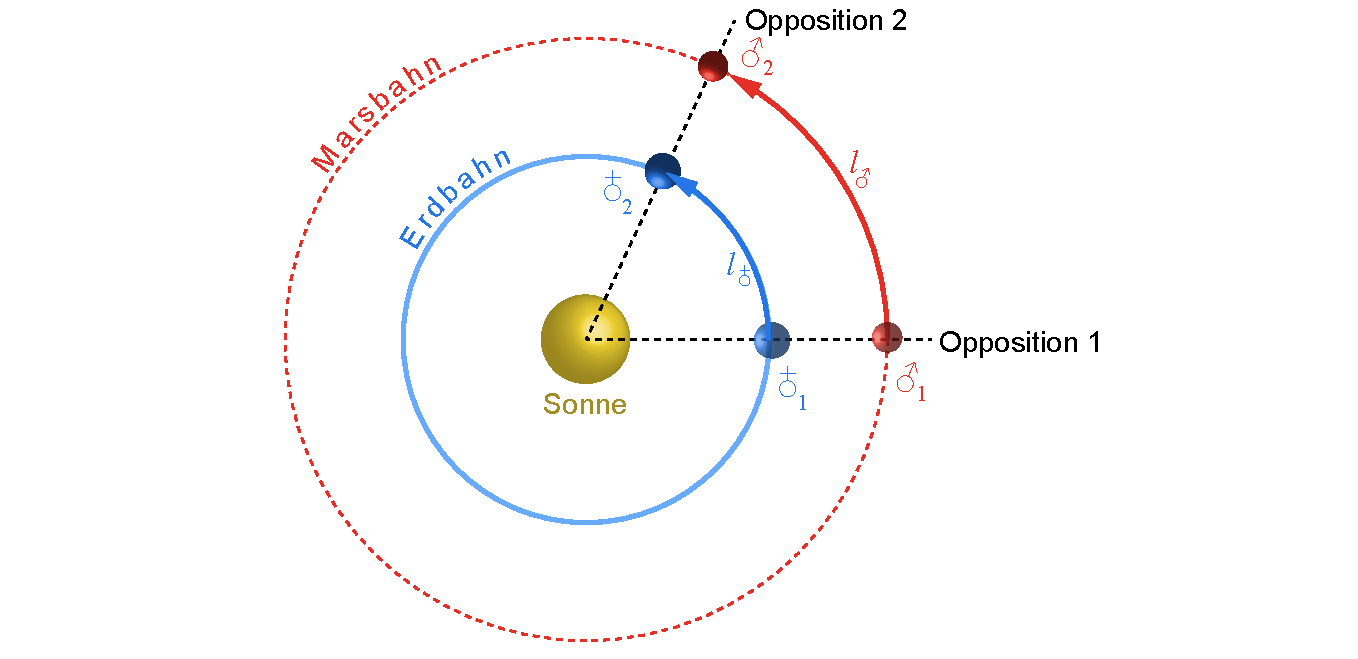
\includegraphics[width=0.9\columnwidth]{Mars_Erde_Umlauf.pdf}%
\caption{Zur Berechnung der siderischen Umlaufzeit des Mars}%
\label{abb:hm_sideric_period_mars}%
\end{figure}
Die Differenz beider L�ngen muss aber wieder $2\pi$ sein.
Daher gilt
\begin{equation*}
	\Delta l= l_{\earth} - l_{\mars} = 2\pi = T_{\text{syn},\mars} \,\lk \omega_{\earth} - \omega_{\mars}\rk = T_{\text{syn},\mars}\, 2\pi\, \lk\frac{1}{T_{\earth}}-\frac{1}{T_{\mars}}\rk ~, 
\end{equation*}
woraus mit $T_{\text{syn},\mars}\!\approx\!779.94\:\text{d}$ und $T_{\earth}\!\approx\!365.256\:\text{d}$ folgt:
\begin{align*}
T_{\mars} = \frac{{T_{\text{syn},\mars}}\, T_{\earth}}{T_{\text{syn},\mars} - T_{\earth}} = 686.980\:\text{d} ~~.\\
\end{align*}
\end{sol}
\textcolor{blue} {$\rightarrow$ zur} \probref{hm_sideric_period_mars}.\\
\noindent\rule[1ex]{\textwidth}{0.5pt} \newpage


%%%-----------------------------------------------------------------------------------------------------------

\subsection{�bungen zur Kepler-Gleichung}

\medskip

%-----------------------------------------------------------------------------------------------------------

\begin{sol}{prob:hm_laplace}\label{lsg:hm_laplace} %�bung4
\textbf{Laplace-Integral} \\
\begin{enumerate}[(i)]
	\item Wir starten von 
\begin{align*}
\vec{L} \times \ddot{\vec{r}} &= \lk \vec{r} \times \dot{\vec{r}}\rk \times \lk \frac{-\mu_\text{G}}{r^3} \rk\, \vec{r} \\
															&= \frac{\mu_\text{G}}{r^3}\,\vec{r}\times \lk \vec{r} \times \dot{\vec{r}}\rk
\end{align*}
Mit der Vektoralgebra-Beziehung 
\begin{equation*}
\vec{a}\times(\vec{b}\times\vec{c}) = \vec{b}(\vec{a}\cdot\vec{c}) - \vec{c}(\vec{a}\cdot\vec{b}) ~~.
\end{equation*}
folgt
\begin{align*}
\vec{L} \times \ddot{\vec{r}} &= \frac{\mu_\text{G}}{r^3} \lek \vec{r}(\vec{r}\cdot\dot{\vec{r}})-\dot{\vec{r}}(\vec{r}\cdot\vec{r}) \rek \\
															&= \frac{\mu_\text{G}}{r^3} \lek \vec{r}(\vec{r}\cdot\dot{\vec{r}})-\dot{\vec{r}}\,r^2\rek  ~.
\end{align*}
In Polarkoordinaten geschrieben ($\vec{r}=r\vec{e}_r$, $\dot{\vec{r}}=\dot{r}\vec{e}_r + r\dot{\vartheta}\vec{e}_\vartheta$) und wegen $\vec{e}_r\!\perp\!\vec{e}_\vartheta$ wird daraus
\begin{align}
\vec{L} \times \ddot{\vec{r}} &= \frac{\mu_\text{G}}{r^3} \lek \vec{r}(r\cdot \dot{r}) - \dot{\vec{r}}(r^2)\rek \nonumber\\
															&= \frac{\mu_\text{G}}{r^2} \dot{r}\,\vec{r} - \frac{\mu_\text{G}}{r}\,\dot{\vec{r}} = -\frac{\D}{\D t} \lk \frac{\mu_\text{G}}{r} \,\vec{r} \rk ~~.\label{eq:hm_laplace_lsg1} 
\end{align}
Die linke Seite kann wegen $\vec{L}\!=\!\vec{const}$ als Zeitableitung geschrieben werden:
\begin{equation*}
\vec{L} \times \ddot{\vec{r}} = \frac{\D }{\D t} \lk \vec{L} \times \dot{\vec{r}}\rk ~~,
\end{equation*}
woraus wir mit \eqref{eq:hm_laplace_lsg1}
\begin{align*}
\frac{\D }{\D t} \lk \vec{L}\times\dot{\vec{r}} + \frac{\mu_\text{G}}{r}\,\vec{r}\rk &= 0 
\end{align*}
erhalten.
Integration mit $-\mu_\text{G}\,\vec{e}$ als Integrationskonstante ergibt
\begin{align*}
\vec{L}\times\dot{\vec{r}} + \frac{\mu_\text{G}}{r}\,\vec{r} &= \vec{const} = -\mu_\text{G} \vec{e}
\end{align*}
und damit schlussendlich
\begin{align}
\vec{e} &= -\frac{1}{\mu_\text{G}} \lk \vec{L}\times\dot{\vec{r}} + \frac{\mu_\text{G}}{r}\,\vec{r} \rk  ~~. \label{eq:hm_laplace_lsg2}
\end{align}
\medskip
\item Wir zeigen nun, dass 
\begin{equation*}
\mu_\text{G}^2(e^2-1) = 2HL^2 ~~.
\end{equation*}
Dazu bilden wir ausgehend von \eqref{eq:hm_laplace_lsg2} das Betragsquadrat:
\begin{align*}
\lk -\mu_\text{G} \vec{e} \rk^2 &= \lk \vec{L}\times\dot{\vec{r}} + \frac{\mu_\text{G}}{r}\,\vec{r} \rk^2 \\
\Rightarrow \mu_\text{G}^2e^2 &= \lk \vec{L}\times\dot{\vec{r}} \rk^2 + \frac{2\mu_\text{G}}{r}\,\vec{r} \lk \vec{L}\times\dot{\vec{r}} \rk + \frac{\mu_\text{G}^2}{r^2}\,\vec{r}^2 \\
															&= \lek (\vec{r}\times\dot{\vec{r}})\times\dot{\vec{r}} \rek^2 + \frac{2\mu_\text{G}}{r}\,\vec{r} \lk \vec{L}\times\dot{\vec{r}} \rk + \mu_\text{G}^2 \\
															&= [\underbrace{(\vec{r}\cdot\dot{\vec{r}})\dot{\vec{r}}}_{0} - \underbrace{(\dot{\vec{r}}\cdot\dot{\vec{r}})}_{\dot{r}^2=v^2}\vec{r}]^2 + \frac{2\mu_\text{G}}{r}\,\vec{r} \lek (\vec{r}\times\dot{\vec{r}})\times\dot{\vec{r}} \rek + \mu_\text{G}^2\\
															&= v^4 r^2 + \frac{2\mu_\text{G}}{r}\,\vec{r} [ (\underbrace{\vec{r}\cdot\dot{\vec{r}})\dot{\vec{r}}}_{0} - \dot{\vec{r}}^2\vec{r} ] + \mu_\text{G}^2 \nonumber \\ 
															&= v^4 r^2 - \frac{2\mu_\text{G}}{r}\,v^2 r^2 + \mu_\text{G}^2 \nonumber 
\end{align*}															
\begin{align}													
\Rightarrow \mu_\text{G}^2 \lk e^2-1\rk &= v^4 r^2 - 2 \mu_\text{G} v^2 r ~~. \label{eq:hm_laplace_lsg3}
\end{align}
Wir benutzen jetzt die Definition $2 H\!\equiv\!v^2-(2\mu_\text{G}/r)$ und $L\!=\!\abs{\vec{L}}\!=\!\abs{\vec{r}\times \vec{v}}\!=\! rv$ und erhalten als Zwischenergebnis
\begin{align*}
2HL^2 = \underbrace{\lk v^2 - \frac{2\mu_\text{G}}{r}\rk}_{2 H} \underbrace{\lk r^2 v^2\rk}_{L^2} = v^4r^2 - 2\mu_\text{G}v^2 r ~~.
\end{align*}
was wir in \eqref{eq:hm_laplace_lsg3} einsetzen, woraus schlie�lich folgt:
\begin{equation*}
\mu_\text{G}^2 \lk e^2-1\rk  = 2 HL^2~~.
\end{equation*}
\end{enumerate}
\end{sol}
\textcolor{blue} {$\rightarrow$ zur} \probref{hm_laplace}.\\
\noindent\rule[1ex]{\textwidth}{0.5pt} \newpage

%-----------------------------------------------------------------------------------------------------------

\begin{sol}{prob:hm_wahre_anomalie}\label{lsg:hm_wahre_anomalie} %�bung5
\textbf{Wahre Anomalie}\\ \\
Wir starten von der Definition der exzentrischen Anomalie \eqref{eq:hm_exzentrische_Anomalie}:
\begin{equation*}
r(t) = a \lk 1-e\,\cos E\rk 
\end{equation*}
und benutzen dann \figref{hm_geom_abl_kepler}, so dass
\begin{align}
\overline{\text{NZ}} \equiv \overline{x}_\text{P} &= \overline{\text{ON}} - \overline{\text{OZ}} \nonumber\\
																						 &= a\cos E - ae \nonumber\\
																						 &= a (\cos E -e) \nonumber\\
\Rightarrow \cos\upsilon = 	\frac{\overline{x}_\text{P}}{r} &= \frac{\cos E-e}{1-e\cos E} ~~. \label{eq:hm_wa_lsg1}
\end{align}
Zun�chst schreiben wir \eqref{eq:hm_wa_lsg1} um in
\begin{align}
1-\cos \upsilon &= \frac{1-e\cos E - \cos E + e}{1-e\cos E} = \frac{(1+e)(1-\cos E)}{1-e\cos E} ~~, \label{eq:hm_wa_lsg2}\\
1+\cos \upsilon &= \frac{1-e\cos E + \cos E - e}{1-e\cos E} = \frac{(1-e)(1+\cos E)}{1-e\cos E} ~~. \nonumber
\end{align}
Um auf den halben Winkel in \eqref{eq:hm_nu(t)_alternativ} zu kommen, nutzen wir die Winkelfunktionsbeziehungen
\begin{align*}
1-\cos x &= 2\sin^2\lk\frac{x}{2}\rk ~~, \\
1+\cos x &= 2\cos^2\lk\frac{x}{2}\rk ~~ 
\end{align*}
und benutzen diese in \eqref{eq:hm_wa_lsg2}.
Wir erhalten sofort nach Quotientenbildung und Wurzelziehen
\begin{align*}
\lk 1 - e\, \cos E\rk \;2 \sin^2\lk\frac{\upsilon}{2}\rk &= 2(1+e)\sin^2\lk\frac{E}{2}\rk ~~,\\
\lk 1 - e\, \cos E\rk \;2 \cos^2\lk\frac{\upsilon}{2}\rk &= 2(1-e)\cos^2\lk\frac{E}{2}\rk ~~,\\
   \rightarrow~~ \tan\lk\frac{\upsilon}{2}\rk &= \sqrt{\frac{1+e}{1-e}}\,\tan\lk\frac{E}{2}\rk~~.
\end{align*}
\end{sol}
\textcolor{blue} {$\rightarrow$ zur} \probref{hm_wahre_anomalie}.\\
\noindent\rule[1ex]{\textwidth}{0.5pt} \newpage

%-----------------------------------------------------------------------------------------------------------

\begin{sol}{prob:hm_bwglg_hyp_parab}\label{lsg:hm_bwglg_hyp_parab} %�bung6
\textbf{Bewegungsgleichungen f�r Hyperbel und Parabel} \\
\begin{enumerate}[(i)]
	\item \emph{Hyperbel}\\
	Diese Herleitung erfolgt analog zur Kepler-Gleichung f�r die Ellipse.
        Man f�hrt lediglich anstelle der Hilfsgr��e \anf{exzentrische Anomalie} eine \anf{hyperbolische exzentrische Anomalie} $E_\text{hyp}$ ein.
        Man beachte dabei, dass bei einer Hyperbel $a\!<\!0$ ist.
        Zudem ben�tigen wir f�r die weitere Rechnung folgende Beziehungen f�r Hyperbelfunktionen:
\begin{align*}
\sinh^2x &= \cosh^2x-1 ~~, \\
\sinh x &= \frac{\D }{\D x} \cosh x ~~,\\
\cosh x &= \frac{\D }{\D x} \sinh x ~~.
\end{align*}
Wir starten zun�chst mit
\begin{align}
r &= a_\text{hyp} (1-e\cosh E_\text{hyp}) \nonumber \\
  &= \abs{a_\text{hyp}} (e\cosh E_\text{hyp} - 1) \label{eq:hm_hyplsg1} 
\end{align}
und bilden die zeitliche Ableitung, die wir anschlie�end quadrieren:
\begin{align}
\frac{\D r}{\D t} =&\, +\abs{a_\text{hyp}}e \sinh E_\text{hyp}\,\lk\frac{\D E_\text{hyp}}{\D t}\rk  \nonumber \\ 
\lk\frac{\D r}{\D t}\rk^2 =&\, +\, \abs{a_\text{hyp}}^2 e^2 (\sinh E_\text{hyp})^2 \,\lk\frac{\D E_\text{hyp}}{\D t}\rk^2 ~.\label{eq:hm_hyplsg2}
\end{align}
Dann starten wir wieder mit der Bahngeschwindigkeit in Polarkoordinaten und benutzen \eqref{eq:hm_dot_r_quadrat}, so dass
\begin{align*}
\lk\frac{\D r}{\D t}\rk^2 =&\, \frac{\mu_\text{G}}{r^2} \lk 2r-\frac{r^2}{a_\text{hyp}}\rk -\lk \frac{a_\text{hyp}(1-e^2)}{r^2} \rk\,\mu_\text{G} ~~.
\end{align*}
Wir setzen jetzt f�r $r$ die Beziehung \eqref{eq:hm_hyplsg1} ein und erhalten 
\begin{align*}
\lk\frac{\D r}{\D t}\rk^2 =&\, \frac{\mu_\text{G}}{r^2} \lk \killA{2\abs{a_\text{hyp}} e \cosh E_\text{hyp}} - \killB{2 \abs{a_\text{hyp}}} +\frac{\abs{a_\text{hyp}}^2}{\abs{a_\text{hyp}}} e^2 \cosh^2 E_\text{hyp} \right.\\
&\,\left. +\killB{\frac{\abs{a_\text{hyp}}^2}{\abs{a_\text{hyp}}}} - \killA{\frac{2\abs{a_\text{hyp}}^2}{\abs{a_\text{hyp}}}e\cosh E_\text{hyp}} + \killB{\abs{a_\text{hyp}}} -\abs{a_\text{hyp}} e^2\rk \\
=&\, \frac{\mu_\text{G}}{r^2} \lk \abs{a_\text{hyp}} e^2 \cosh^2 E_\text{hyp} - \abs{a_\text{hyp}} e^2\rk \\
=&\, \frac{\mu_\text{G}}{r^2} \abs{a_\text{hyp}} e^2 \underbrace{\lk \cosh^2 E_\text{hyp} - 1\rk}_{\sinh^2 E_\text{hyp}} ~~, 
\end{align*}
und weiter mit \eqref{eq:hm_hyplsg2}
\begin{align*}
\abs{a_\text{hyp}}^{\killA{2}} \killA{e^2 \sinh^2 E_\text{hyp}} \,\lk \frac{\D E_\text{hyp}}{\D t}\rk^2 &= \frac{\mu_\text{G}}{r^2} \killA{\abs{a_\text{hyp}} e^2 \sinh^2 E_\text{hyp}} \\
\Rightarrow r \lk \frac{\D E_\text{hyp}}{\D t}\rk &= \sqrt{\frac{\mu_\text{G}}{\abs{a_\text{hyp}}}} ~~.
\end{align*}
Wir setzen wieder f�r $r$ die Beziehung \eqref{eq:hm_hyplsg1} ein und bekommen
\begin{align*}
\abs{a_\text{hyp}} (e\cosh E_\text{hyp} - 1)\,\D E_\text{hyp} &= \sqrt{\frac{\mu_\text{G}}{\abs{a_\text{hyp}}}} \,\D t ~~,
\end{align*}
woraus nach Integration 
\begin{align}
e \sinh E_\text{hyp} - E_\text{hyp}  &= \sqrt{\frac{\mu_\text{G}}{\abs{a_\text{hyp}}^3}} (t-t_0) = M_\text{hyp}(t-t_0) ~~  \label{eq:hm_hyplsg3}
\end{align}
eine hyperbolische modifizierte Kepler-Gleichung resultiert.
Die L�sung dieser Gleichung erfolgt ebenfalls numerisch durch Iteration oder Reihenentwicklung.\\

\item \emph{Parabel}\\
Bei der Parabel ist die Situation interessanterweise etwas einfacher.
Wir wissen ja, dass f�r die Parabel $e\!=\!1$ ist.
Somit arbeiten wir mit dem Parameter $p$.
Wir starten von der Kegelschnittgleichung \eqref{eq:hm_kegelschnitt}:
\begin{equation*}
r(\upsilon) = \frac{L^2}{\mu_\text{G}}\,\frac{1}{1+\cos \upsilon} = \frac{p}{1+\cos \upsilon} ~~.
\end{equation*}
Andererseits ist noch wegen \eqref{eq:hm_drehimp_z} $L\!=\!r^2\dot{\upsilon}$, so dass wir fortfahren mit
\begin{align*}
\frac{\D \upsilon}{\D t} &= \frac{L}{r^2} \Rightarrow r^4\,\lk\frac{\D \upsilon}{\D t}\rk^2 = L^2 = \mu_\text{G}p \\
\Rightarrow \frac{\D \upsilon}{\D t} &= \sqrt{\mu_\text{G} p} \lk\frac{1}{r^2}\rk = \sqrt{\mu_\text{G} p}\,\lk\frac{(1+\cos\upsilon)^2}{p}\rk^2 \\
\Rightarrow \D \upsilon &= \sqrt{\frac{mu_\text{G}}{p^3}} \lek 2\cos^2\lk\frac{\upsilon}{2}\rk\rek^2 \,\D t ~~,
\end{align*}
wobei wir in der letzten Zeile die Beziehung $1+\cos x\!=\!2\cos^2(x/2)$ verwendet haben.
Damit erhalten wir nach Trennung der Variablen
\begin{equation*}
\frac{1}{2} \lk \,\frac{1}{\cos^4 \lk\frac{\upsilon}{2}\rk} \rk\,\D \lk\frac{\upsilon}{2}\rk  = \sqrt{\frac{\mu_\text{G}}{p^3}}\,\D t ~~.
\end{equation*}
In Integraltabellen findet man $\int (\cos^{-4} u)\,\D u \!=\! \tan u + (1/3)\tan^3 u + c$, was man leicht durch Differenzieren pr�fen kann.
Damit erhalten wir nun eine Bestimmungsgleichung f�r $\upsilon$:
\begin{equation*}
\tan\lk\frac{\upsilon}{2}\rk + \frac{1}{3}\tan^3\lk\frac{\upsilon}{2}\rk = 2 \sqrt{\frac{\mu_\text{G}}{p^3}} (t-t_0)~~.
\end{equation*}
Aus der Parabelgleichung folgt f�r $\upsilon\!=\!0$ die Periheldistanz $q$ zu
\begin{equation*}
q = \frac{p}{1+\cos(0)} = \frac{p}{2}
\end{equation*}
und daraus die sogenannte Barkersche Gleichung f�r die wahre Anomalie der Bahn der Parabel
\begin{equation}
\tan\lk\frac{\upsilon}{2}\rk  + \frac{1}{3} \tan^3\lk\frac{\upsilon}{2}\rk  = \sqrt{\frac{4\mu_\text{G}}{8q^3}} (t-t_0) = \sqrt{\frac{\mu_\text{G}}{2q^3}} (t-t_0)~~.
\label{eq:hm_BarkerGleichung01}
\end{equation}
Das ist noch eine transzendente Gleichung in $\upsilon$.
Setzt man aber $\tan(\upsilon/2)\!=\!u$, so wird daraus
\begin{equation}
u+\frac{1}{3}u^3 = M_\text{P}(t-t_0)~~, \label{eq:hm_BarkerGleichung02}
\end{equation}
gl�cklicherweise eine mit den bekannten Formeln f�r kubische Gleichungen analytisch l�sbare Form.
Mit
\begin{equation*}
A = \frac{3}{2} \sqrt{\frac{\mu_\text{G}}{2q^3}} (t-t_0)A ~~~\text{und}~~~B = \sqrt[3]{A+\sqrt{A^2+1}}
\end{equation*}
findet man:
\begin{equation}
   \upsilon = 2\arctan{(\lk b - \frac{1}{B}\rk }\,. \label{eq:hm_BarkerGleichung03}
\end{equation}

Im Gegensatz zur Ellipse und Hyperbel hat also der Spezialfall der Parabel\index{Parabel} eine geschlossene analytische L�sung.
Wir werden dieser Barkerschen Gleichung\index{Barkersche Gleichung} in modifizierte Form bei der Berechnung von Kometenbahnen wieder begegnen.
\end{enumerate}
\end{sol}
\textcolor{blue} {$\rightarrow$ zur} \probref{hm_bwglg_hyp_parab}.\\
\noindent\rule[1ex]{\textwidth}{0.5pt} \newpage

%-----------------------------------------------------------------------------------------------------------

\begin{sol}{prob:hm_iteration}\label{lsg:hm_iteration} %�bung7
\textbf{Iteration} \\ \\
Die Rechnungen sind im Detail in \mlhmref{KeplerVergleich.m} ausgef�hrt. 
\end{sol}
\textcolor{blue} {$\rightarrow$ zur} \probref{hm_iteration}.\\
\noindent\rule[1ex]{\textwidth}{0.5pt} \newpage

%-----------------------------------------------------------------------------------------------------------

\begin{sol}{prob:hm_bessel}\label{lsg:hm_bessel} %�bung8
\textbf{Bessel-Reihe} \\ \\
Die Rechnungen sind im Detail im \mscr{} \mlhmref{Besselreihe.m} ausgef�hrt. 
\end{sol}
\textcolor{blue} {$\rightarrow$ zur} \probref{hm_bessel}.\\
\noindent\rule[1ex]{\textwidth}{0.5pt} \newpage

%-----------------------------------------------------------------------------------------------------------

\begin{sol}{prob:hm_alternative_MPG}\label{lsg:hm_alternative_MPG} %�bung9
\textbf{Alternative Herleitung der Mittelpunktsgleichung} \\ \\
Im Beispiel \ref{bsp:mittelpktglg} hatten wir die Mittelpunktsgleichung �ber die Bessel-Reihe hergeleitet.
Wir wollen hier nun Herleitung �ber die Iterationsl�sung nach Kapitel \ref{kap:iteration_kepler} wiederholen und folgen dabei der eleganten Darstellung in \cite{Smart1986}. Wir starten mit \eqref{eq:hm_nu(t)_alternativ} (siehe auch \probref{hm_wahre_anomalie}):
\begin{equation*}
\tan \lk \frac{\upsilon}{2} \rk = \sqrt{\frac{1+e}{1-e}}\,\tan\lk\frac{E}{2}\rk ~~.
\end{equation*}
Wir setzen $\sin\alpha\!=\!e$, da $0\!\leq\! e\!\leq\! 1$, was aus $0\!\leq\!\alpha\!\leq\!\pi$ folgt.
Mit der Identit�t 
\begin{align*}
1 \pm \sin\alpha &= 1 \pm \frac{2 \tan\lk\frac{\alpha}{2}\rk}{1+\tan^2\lk\frac{\alpha}{2}\rk} = \frac{1 \pm 2 \tan\lk\frac{\alpha}{2}\rk+\tan^2\lk\frac{\alpha}{2}\rk}{1+\tan^2\lk\frac{\alpha}{2}\rk} \\
                 &= \frac{{\lk 1 \pm \tan\lk\frac{\alpha}{2}\rk \rk}^2}{1+\tan^2\lk\frac{\alpha}{2}\rk}
\end{align*}
erh�lt man
\begin{equation}
\tan \lk \frac{\upsilon}{2} \rk  = \frac{1+\tan\lk\frac{\alpha}{2}\rk}{1-\tan\lk\frac{\alpha}{2}\rk}\,\tan\lk\frac{E}{2}\rk = \frac{1+x}{1-x}\,\tan\lk\frac{E}{2}\rk~~. \label{eq:hm_lsg_mpg_1}
\end{equation}
Wir benutzen nun die Euler-Gleichungen $\cos\theta\!=\!1/2 \lk \E^{\im\theta}+\E^{-\im\theta}\rk$ und $\sin\theta\!=\!1/(2\im)\lk\E^{\im\theta}-\E^{-\im\theta}\rk$ und schreiben mit dem Tangens des halben Winkels $\upsilon$ und analog f�r den Tangens des halben Winkel $E$ die Beziehung f�r die wahre Anomalie als
\begin{equation*}
\tan \lk \frac{\upsilon}{2} \rk = \frac{\E^{+\im\upsilon/2} - \E^{-\im\upsilon/2}}{i\lk\E^{+\im\upsilon/2} + \E^{-\im\upsilon/2}\rk} = \frac{\E^{\im\upsilon}-1}{i\lk \e^{\im\upsilon} + 1\rk} \frac{\killA{\E^{-\im\upsilon/2}}}{\killA{\E^{-\im\upsilon/2}}}~~,
\end{equation*}
woraus mit \eqref{eq:hm_lsg_mpg_1} folgt
\begin{equation}
\frac{\E^{\im\upsilon}-1}{\E^{\im\upsilon}+1} = \frac{1+x}{1-x}\,\frac{\E^{\im E}-1}{\E^{\im E}+1}~~.
\label{eq:hm_lsg_mpg_2}
\end{equation}
Wir setzen nun $\E^{\im\upsilon}\!\equiv\!\E^q$ und die rechte Seite gleich $Q$.
Damit ergibt sich vereinfacht
\begin{align}
\E^q -1 &= Q\lk \E^q+1\rk \nonumber\\
\E^q \lk 1-Q\rk &= Q+1  \nonumber\\
\Rightarrow \E^{\im \upsilon} &= -\frac{Q+1}{Q-1} = \frac{\E^{\im E}-x}{1-x\E^{\im E}} \nonumber\\
															 &= \E^{\im E} \lk \frac{1-x\E^{-\im E}}{1-x\E^{+\im E}} \rk ~~. \label{eq:hm_lsg_mpg_3}
\end{align}
Wir bilden davon den Logarithmus und erhalten
\begin{equation}
\im\upsilon = \im E + \ln\lk1-x\E^{-\im E}\rk - \ln\lk1-x\E^{+\im E}\rk ~~.
\label{eq:hm_lsg_mpg_4}
\end{equation}
Da $x\!=\!\tan(\alpha/2)$ und $\alpha\!=\!\arcsin(e)$, ist $\alpha$ definitiv kleiner als $\pi/2$ und damit $0\!<\!x^e\!<\!1$.
Wir benutzen jetzt die Reihenentwicklung $\ln(1-z)\!=\!z-z^2/2-z^3/3-z^4/4-\ldots$ und erhalten 
\begin{align}
\im\upsilon &= \im E + x\E^{\im E} - x\E^{-\im E} + \frac{x^2}{2}\E^{2\im E} - \frac{x^2}{2}\E^{-2\im E} + \frac{x^3}{3}\E^{3\im E} - \frac{x^3}{3}\E^{-3\im E} - \ldots \nonumber\\
\Rightarrow \im\upsilon &= \im \lek E + \lk 2x\sin E + x^2 \sin(2E) + \frac{2}{3} x^3 \sin(3E) + \ldots \rk \rek~~. \label{eq:hm_lsg_mpg_5}
\end{align}
Jetzt m�ssen wir noch $x$ re-substituieren gem��
\begin{equation*}
x = \tan\lk\frac{\alpha}{2}\rk = \frac{\sin^2\lk\frac{\alpha}{2}\rk}{\sin\lk\frac{\alpha}{2}\rk \cos\lk\frac{\alpha}{2}\rk} = \frac{1-\cos^2\lk\frac{\alpha}{2}\rk}{\frac{1}{2}\sin\alpha} = \frac{2\lk1-\cos^2\lk\frac{\alpha}{2}\rk\rk}{e} ~~.
\end{equation*}
Wiederum benutzen wir die Identit�t $2\,\cos^2(\alpha/2)\!=\!(1+\cos\alpha)$ und erhalten
\begin{equation*}
x = \frac{1-\cos\alpha}{e} = \frac{1-\sqrt{1-\sin^2\alpha}}{e} = \frac{1-\sqrt{1-e^2}}{e} ~~.
\end{equation*}
Wir entwickeln nun den Ausdruck in der Wurzel nach kleinen $e$:
\begin{align*}
x &= \frac{1}{e} \lk 1- \lk 1-\frac{e^2}{2} - \frac{e^4}{8} - \frac{e^6}{16} - \ldots \rk\rk \\
  &= \frac{e}{2} + \frac{e^3}{8} + \frac{e^5}{16} + \ldots ~~.
\end{align*}
Dies setzen wir nun in \eqref{eq:hm_lsg_mpg_5} ein und erhalten schlie�lich bis zur 3. Ordnung von $e$
\begin{equation}
\upsilon = E + \lk e+\frac{e^3}{4} \rk\sin(E) + \frac{e^2}{4} \sin(2E) + \frac{e^3}{12} \sin(3E) + \mathcal{O}(e^4) ~~.
\label{eq:hm_lsg_mpg_6}
\end{equation}
Nun m�ssen wir noch die Sinus-Werte der unbekannten exzentrischen Anomalie $E$ durch die bekannte mittlere Anomalie $M$ ausdr�cken, um die gesuchte Gleichung f�r $\upsilon-M$ zu erhalten.
Dazu nutzen wir das Iterationsergebnis \eqref{eq:hm_entwicklung_4Ord}, brauchen aber nur die Entwicklung bis $e^2$, da in \eqref{eq:hm_lsg_mpg_6} alle $\sin kE$-Funktionen mindestens mit $e$ multipliziert werden.
Wir bekommen
\begin{equation}
E = M+\lk e-\frac{e^3}{8}\rk\sin(M) + \frac{e^2}{2}\sin(2M) + \frac{3}{8} e^3\sin(3M) + \ldots ~~.
\label{eq:hm_lsg_mpg_7}
\end{equation}
Wir brauchen aber nur Terme bis zur Ordnung $e^2$ mitzunehmen, da in \eqref{eq:hm_lsg_mpg_5} mindestens mit der Potenz 1 vo $e$ multipliziert wird. Wir k�nnen also schreiben:
\begin{equation*}
\sin E \approx \sin\lk M+e\sin(M) +\frac{e^2}{2}\sin(2M)\rk \,.
\end{equation*}
Mit der N�herung f�r kleine Winkel\\
$\sin x\!\approx\!x$, $\cos x\!\approx\!1-\frac{1}{2}x^2$,
den Additionstheoremen der Trigonometrie und der Beziehung $\sin^3 x = \frac{3}{4}\sin x -\frac{1}{4}\sin(3x) $ ergibt das dann in Ordnungen bis $e^2$:
\begin{align*}
\sin(E)  &= \sin(M)\, \cos\lk e\sin(M) +\frac{e^2}{2}\sin(2M)\rk + \cos(M)\,\sin\lk e\sin(M) +\frac{e^2}{2}\sin(2M)\rk \\
         &\approx \sin(M)\,\lek 1- \frac{1}{2}e^2\sin^2(M) \rek + \cos(M)\,\lek e\sin(M)+\frac{e^2}{2}\sin(2M) \rek \\
         &= \sin(M) + \frac{1}{2}e\sin(2M) + \frac{e^2}{2} \lek \sin(2M)\cos(M) - \sin^3(M) \rek \\
         &= \lk 1- \frac{e^2}{8} \rk \sin(M) + \frac{1}{2}e\sin(2M)  + \frac{3}{8}e^2\sin(3M) \,.
\end{align*}
Analog erhalten wir:
\begin{align*}
\sin(2E) &\approx \sin(2M) + e(\sin(3M) - \sin M)\,, \\
\sin(3E) &\approx \sin 3M ~~.
\end{align*}
Die $\sin(E),\, \sin(2E),\, \sin(3E)$-N�herungen setzen wir in \eqref{eq:hm_lsg_mpg_6} ein und erhalten schlie�lich die Mittelpunktsgleichung \eqref{eq:hm_mpglg_nu-M} bis zur Ordnung $e^3$:
\begin{equation*}
\upsilon-M = \lk 2e-\frac{e^3}{2}k \rk\sin(M) + \frac{5e^2}{4} \sin(2M) + \frac{13e^3}{12}\sin(3M) ~~.
\end{equation*}
Auch hier empfehlen wir als weitere �bung die Entwicklung bis mindestens zum Term mit $e^4$ bzw. $\sin(4M)$ zu berechnen.\\
\end{sol}
\textcolor{blue} {$\rightarrow$ zur} \probref{hm_alternative_MPG}.\\
\noindent\rule[1ex]{\textwidth}{0.5pt} \newpage


%%%-----------------------------------------------------------------------------------------------------------

\subsection{�bungen zur Bewegung der Erde in der Ekliptik und zu Himmelsbeobachtungen von der Erde}

\medskip

%-----------------------------------------------------------------------------------------------------------

\begin{sol}{prob:hm_erdbahn_im_jahr}\label{lsg:hm_erdbahn_im_jahr} %�bung10
\textbf{Die Erdbahn im Laufe eines Jahres} \\
\begin{enumerate}[(1)]
	\item Die Perihel- bzw. Apheldistanzen berechnen sich zu
	\begin{align*}
  r_\text{per} &= \frac{p}{1+e\cos\upsilon}\bigg|_{\upsilon=0} = \frac{a(1-e^2)}{1+e} = a(1-e) \approx 147.098\cdot 10^6\:\text{km} ~~,\\
	 r_\text{aph} &= \frac{p}{1+e\cos\upsilon}\bigg|_{\upsilon=\pi} = a(1+e) \approx 152.098\cdot 10^6\:\text{km} ~~.
	\end{align*}
	Die Erdentfernung schwankt also um insgesamt $5\cdot 10^6\:$km.
	\item Wir wollen die mittlere Entfernung berechnen.
          Dazu gibt es zwei M�glichkeiten: den \emph{r�umlichen} Mittelwert der Entfernung zwischen Brennpunkt (Sonne) und Bahn und den \emph{zeitlichen} Mittelwert. 
		\begin{itemize}
		\item Wir beginnen mit dem r�umlichen Mittelwert und schreiben
		 \begin{align}
			\bar{r} &= \frac{1}{2\pi} \int\limits_{0}^{2\pi} r(\upsilon)\,\D\upsilon= \frac{p}{2\pi}\,2\,\int\limits_0^\pi \frac{1}{1+e\cos \upsilon}\,\D\upsilon \label{eq:hm_erdbahn_lsg_1} \\
			         &\stackrel{\text{\cite{Gradshteyn1980}}}{=} \frac{p}{\pi}\,\frac{2}{\sqrt{1-e^2}}\,\arctan\lk \sqrt{\frac{1-e}{1+e}} \,\underbrace{\tan\lk \frac{\upsilon}{2}\rk}_{\rightarrow\infty} \rk\Bigg|_0^\pi = \frac{2p}{\pi\sqrt{1-e^2}} \,\underbrace{\arctan(\infty)}_{\rightarrow\pi/2} \nonumber \\
                                 &= \frac{p}{\sqrt{1-e^2}} = \frac{a(1-e^2)}{\sqrt{1-e^2}} = a\sqrt{\frac{(1-e^2) \killA{(1-e^2)}}{\killA{(1-e^2)}}} = a\sqrt{1-e^2} = b ~~.\nonumber
		 \end{align}
		Dieser Mittelwert ist also gleich der kleinen Halbachse.
		\item Wir berechnen jetzt den zeitlichen Mittelwert unter Benutzung von $T\!=\!T_\text{sid}$:
	\begin{align}
	\bar{r}^t &= \frac{1}{T_\text{sid}} \int\limits_{0}^{T_\text{sid}} r(t)\,\D t = \frac{1}{T}\int\limits_0^{2\pi} r(\upsilon) \,\underbrace{\frac{\D t}{\D \upsilon}}_{1/\dot{\upsilon}}\,\D\upsilon = \frac{1}{T}\int\limits_0^{2\pi} \frac{r(\upsilon)}{\dot{\upsilon}}\,\D\upsilon ~.\label{eq:hm_erdbahn_lsg_2}
	\end{align}
Unter Benutzung des Drehimpulssatzes $1/\dot{\upsilon}\!=\!r^2/L$ erh�lt man zun�chst
		\begin{equation*}
		\bar{r}^t = \frac{1}{TL} \int\limits_0^{2\pi} r^3(\upsilon)\,\D\upsilon = \frac{1}{TL}\int\limits_0^{2\pi} \frac{p^3}{(1+e\cos\upsilon)^3}\,\D\upsilon = \frac{2p^3}{TL}\int\limits_0^{\pi} \frac{1}{(1+e\cos\upsilon)^3}\,\D\upsilon ~~.
		\end{equation*}
		Mit den Integraltabellen aus \cite{Gradshteyn1980} ergibt sich damit
		\begin{equation}
		\bar{r}^t = \frac{2p^3}{TL}\,\pi\,\frac{\lk 1+\frac{e^2}{2}\rk}{(1-e^2)^{5/2}} ~~. \label{eq:hm_erdbahn_lsg_4}
		\end{equation}
		Wir benutzen jetzt den Fl�chensatz f�r einen ganzen Umlauf $TL\!=\! 2A_\text{Ellipse}\!=\!2\pi\,a b$.
                Mit \eqref{eq:hm_erdbahn_lsg_4} erhalten wir dann unter Benutzung von $\sqrt{1-e^2}\!=\!b/a$
		\begin{align*}
		\bar{r}^t =&\, \frac{\killA{2}p^3}{\killA{2\pi} ab}\,\killA{\pi}\,\lk 1+\frac{e^2}{2}\rk \frac{a^5}{b^5} = \, \frac{a^7 \lk\sqrt{1-e^2}\rk^6}{b^6}\,\lk 1+\frac{e^2}{2}\rk\\
							=&\, \frac{a \overbrace{\lek a \sqrt{1-e^2}\rek^6}^{=b^6}}{b^6}\,\lk 1+\frac{e^2}{2}\rk = \, a \lk 1+\frac{e^2}{2}\rk ~\\
						\text{mit}~ p =& a(1-e^2) ~.
		\end{align*}
Das hei�t, dass die Erde im zeitlichen Mittel mehr als $1\:$AE entfernt ist und zwar um $20886\:$km.
Die kleinere Geschwindigkeit am Aphel f�hrt zu einem l�ngeren Aufenthalt im dortigen Bereich.
	\end{itemize}
	\item Die Jahreszeiten sind kein Effekt der Elliptizit�t der Bahn, sondern werden prim�r durch die Ekliptikneigung und - pr�zession hervorgerufen.
          Wir betrachten dazu die \figref{hm_erdbahn_lsg_1}, in der wir die Projektion der Erdachse auf die Bahnebene (Ekliptik) zeigen.\footnote{Der Richtungseinheitsvektor der Erdachse $\vec{s}_{\text{rot},\earth}$ hat die Komponenten $s_{\text{rot},x}\!=\!\sin\epsilon\cos\alpha$, $s_{\text{rot},y}\!=\!\sin\epsilon\sin\alpha$ und $s_{\text{rot},z}\!=\!\cos\epsilon$, wobei $\alpha$ der Winkel ist, den die Projektion der Erdachse auf die Ekliptik mit der $x$-Achse bildet.
          Die Projektion der Erdachse auf die Ekliptik $\vec{s}_{\text{ek}}$ zeigt also in Richtung des Vektors Sonne zur Position der Wintersonnnenwende.} Definitionsgem�� steht zum �quinoktium die Achse dann in ihrer Ausrichtung senkrecht zur Sonne (\ldots wir schauen von oben auf die Bahnebene). 
\begin{figure}[H]
\centering
	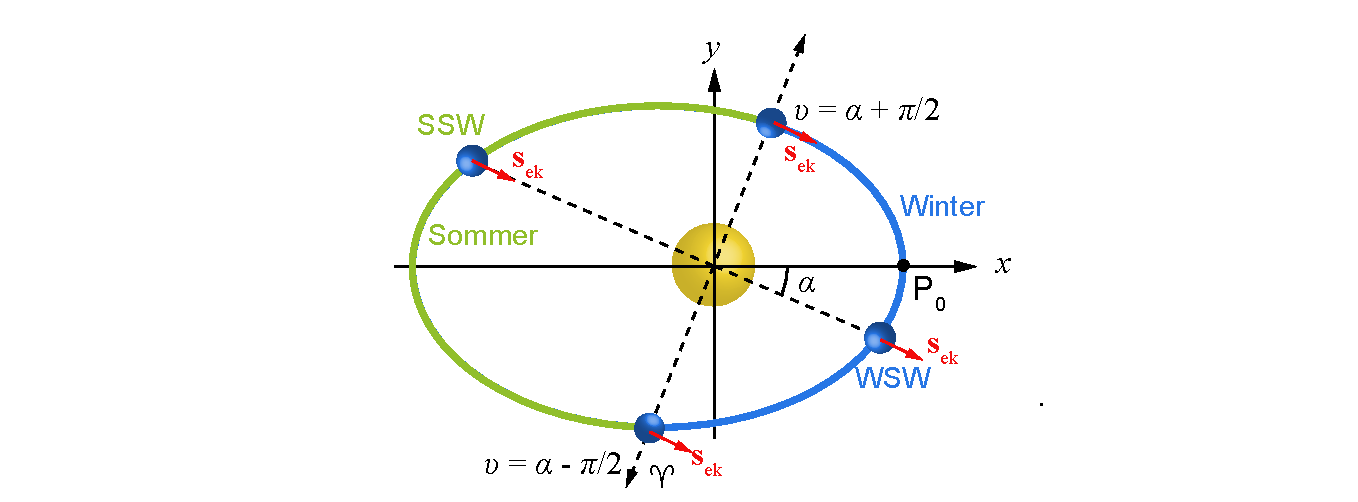
\includegraphics[width=\textwidth]{Erdbahn_im_Jahr_lsg2.pdf}%
	\caption{Erdbahn im Jahresverlauf}%
	\label{abb:hm_erdbahn_lsg_1}%
\end{figure}

	Wir definieren jetzt:
	\begin{align*}
		\text{Nordwinter: }& \alpha - \frac{\pi}{2} \leq \upsilon \leq \alpha+\frac{\pi}{2} ~~,\\
		\text{Nordsommer: }& \alpha + \frac{\pi}{2} \leq \upsilon \leq \alpha+\frac{3\pi}{2} ~~.
	\end{align*}
	Diese Halbjahre sind durch die Richtung der Erdachse gegeben und sind keineswegs gleich lang, wie wir gleich berechnen werden.
        Der gesamte Umlauf ben�tigt nach dem 3. Keplerschen Gesetz $T_\text{ges}\!=\!2\pi \sqrt{a^3/\mu_\text{G}}$.
        Die zeitliche Dauer des Sommerhalbjahrs ergibt sich dann mit Nutzung der Beziehungen
	\begin{align*}
		\frac{\D\upsilon}{\D t} &= \frac{L}{r^2} ~~\text{bzw.} ~~ \D t = \frac{r^2\,\D\upsilon}{L} ~,\;L = \sqrt{a\mu_\text{G}(1-e^2)} ~ \text{und}\;	r^2 = \lek \frac{a(1-e^2)}{1+e\cos\upsilon} \rek^2 ~~
	\end{align*}
	zu
	\begin{align}
   T_\text{Sommer} &= \frac{1}{L} \int\limits_{\alpha+\pi/2}^{\alpha+3\pi/2} r^2 \,\D\upsilon = \frac{a^2\lk 1-e^2\rk^2}{\sqrt{a\mu_\text{G}(1-e^2)}} \,\int\limits_{\alpha+\pi/2}^{\alpha+3\pi/2} \frac{1}{\lk 1+e\cos\upsilon\rk^2}\,\D\upsilon \nonumber\\
									 &= \frac{a^{3/2}\lk 1-e^2\rk^{3/2}}{\sqrt{\mu_\text{G}}} \,\underbrace{\int\limits_{0}^{\pi} \frac{1}{\lek 1-e\sin(\varphi+\alpha)\rek^2} \,\D\varphi}_{\equiv I} ~~, \label{eq:hm_erdbahn_lsg_5}
	\end{align}
	wobei wir $\cos(x+\pi/2)\!=\!-\sin x$ verwendet und $\varphi\!=\!\upsilon-(\alpha+\pi/2)$ gesetzt haben.
        Die L�sung des Integrals $I$ in \eqref{eq:hm_erdbahn_lsg_5} k�nnten wir wieder �ber \cite{Gradshteyn1980} erledigen.
        Wir wollen aber hier f�r kleine $e$ eine Reihenentwicklung durchf�hren:
	\begin{align*}
		I =&\, \int\limits_{0}^{\pi} \frac{1}{\lek 1-e\sin(\varphi+\alpha)\rek^2} \,\D\varphi \\
		  =&\, \int\limits_{0}^{\pi} \lek 1+2e\sin(\varphi+\alpha) + 3e^2\sin^2(\varphi+\alpha) + 4e^3\sin^3(\varphi+\alpha) \rek\,\D\varphi \\
		  =&\, \pi - 2e\cos(\varphi+\alpha) \bigg|_0^\pi + 3e^2 \lek -\frac{1}{4}\sin(2(\varphi+\alpha))+ \frac{1}{2}(\varphi+\alpha) \rek_0^\pi \\
			 &\, + 4e^3 \lek \frac{1}{12}\cos(3(\varphi+\alpha)) - \frac{3}{4}\cos(\varphi+\alpha)\rek_0^\pi \\
			=&\, \pi + 4e\cos\alpha+\frac{3}{2} e^2 \pi - 4e^3\,\frac{1}{6}\cos(3\alpha) + 6e^3\cos\alpha ~~.
	\end{align*}
	Damit erhalten wir
	\begin{align}
	T_\text{Sommer} =&\, \frac{a^{3/2}}{\sqrt{\mu_\text{G}}} \lk 1-\frac{3e^2}{2} + \mathcal{O}(e^4)\rk \lk \pi + 4e\cos\alpha + \frac{3e^2}{2} \pi - \frac{2e^3}{3}\cos (3\alpha) \right.\nonumber\\
	                 &\left. + 6e^3\cos\alpha +\mathcal{O}(e^4)\rk \nonumber\\
	              =&\, \frac{a^{3/2}}{\sqrt{\mu_\text{G}}} \lek \pi - \killA{\frac{3e^2}{2} \pi} + 4e\cos\alpha + \killA{\frac{3e^2}{2} \pi} - \killB{6e^3\cos\alpha} \right.\nonumber\\
                      &\left. -\frac{2e^3}{3}\cos(3\alpha) + \killB{6e^3\cos\alpha} + \mathcal{O}(e^4) \rek \nonumber\\
								=&\, \frac{a^{3/2}}{\sqrt{\mu_\text{G}}} \lek \pi + 4e\cos\alpha - \frac{2e^3}{3}\cos(3\alpha)\rek ~~.\label{eq:hm_erdbahn_lsg_6}
	\end{align}
	Wegen $T_\text{Winter}\!=\! T_\text{ges} - T_\text{Sommer}$ ergibt sich die Differenz der beiden Halbjahre zu
	\begin{align}
		\Delta T &= \frac{T_\text{Sommer} - T_\text{Winter}}{T_\text{ges}} = \frac{2T_\text{Sommer}}{T_\text{ges}}-1 \nonumber \\
		         &= \frac{2a^{3/2}\,\sqrt{\mu_\text{G}}}{\sqrt{\mu_\text{G}}\,2\pi\,a^{3/2}} \lek \pi+4e\cos\alpha-\frac{2e^3}{3}\cos^3(3\alpha)\rek -1 \nonumber \\
						&= \frac{4e}{\pi}\,\cos\alpha-\frac{2e^3}{3\pi}\,\cos(3\alpha) ~~. \label{eq:hm_erdbahn_lsg_7}
	\end{align}
	Die unterschiedliche Dauer der Jahreszeiten h�ngt also von der aktuellen Stellung der Erdachse (innerhalb ihrer Pr�zession) und der Elliptizit�t ab, nicht aber von der Neigung der Ekliptik.
        Der Winkel $\alpha$ ist der Winkel, den die Projektion der Erdachse auf die Ekliptik mit der Apsidenlinie bildet.
        Der Winkel $\alpha$ kann positiv oder negativ sein.
        Zum jetzigen Zeitpunkt (30.01.2021) ist dieser f�r die Erde negativ, da die Wintersonnenwende zeitlich vor dem Periheldurchgang liegt (\figref{hm_erdbahn_lsg_1}).
        Die Pr�zession der Erdachse �ndert sich aber $\alpha$ im Laufe der Zeit, was nach \eqref{eq:hm_erdbahn_lsg_6} bedeutet, dass sich auch die Dauer der Jahreszeiten �ndert. 
	\item Wir wollen jetzt den Eintrag der Sonne w�hrend eines Halbjahres berechnen und damit die Klimaeffekte absch�tzen.
          W�hrend eines Zeitraums $\D t$ erh�lt die Erde die Energie
	\begin{equation*}
	\D H = \frac{P_\text{\astrosun}}{4\pi r^2(\upsilon)}\,\pi R_\text{\earth}^2\,\D t = \frac{R_\text{\earth}^2}{4r^2(\upsilon)}\,P_\text{\astrosun}\,\frac{\D t}{\D\upsilon}\,\D\upsilon ~~,
	\end{equation*}
	wobei $P_\text{\astrosun}$ die Strahlungsleistung der Sonne und $R_\text{\earth}$ der Erdradius ist.
        Wir benutzen den bereits gut bekannten Trick mit dem Drehimpuls (\ldots was w�rden wir nur tun, wenn der keine Konstante w�re \ldots) und erhalten
	\begin{equation*}
	\D H = \frac{R_\text{\earth}^2 P_\text{\astrosun}}{4r^2(\upsilon)}\,\frac{r^2(\upsilon)}{L}\,\D\upsilon = \frac{1}{4}\,\frac{R_\text{\earth}^2 P_\text{\astrosun}}{\sqrt{a\mu_\text{G}(1-e^2)}}\,\D\upsilon ~~.
		\end{equation*}
	Die Energie in einem Jahr ist dann
	\begin{equation}
	H_\text{ges} = \int\limits_0^{2\pi} \D H = \frac{R_\text{\earth}^2 P_\text{\astrosun}}{4\sqrt{\mu_\text{G}}}\,\frac{2\pi}{\sqrt{a(1-e^2)}} = C_\text{H} \frac{2\pi}{\sqrt{a(1-e^2)}}~~,	\label{eq:hm_erdbahn_lsg_8}
	\end{equation}
	worin $C_\text{H}$ eine Konstante ist, die der Strahlungsleistung der Sonne direkt proportional ist.
        Wir k�nnen nat�rlich auch den Energieeintrag f�r ein Halbjahr berechnen:
	\begin{equation*}
	H_\text{Winter} = \int\limits_{\alpha-\pi/2}^{\alpha+\pi/2} \D H = \frac{H_\text{ges}}{2} ~~.
	\end{equation*}
	Danach w�ren die Energieeintr�ge f�r beide Halbjahre gleich gro�.
        Das ist etwas �berraschend, aber verst�ndlich, denn wir haben ja die komplette Querschnittsfl�che der Erde betrachtet, und �ber den Fl�chensatz werden die unterschiedlichen Halbjahresl�ngen zeitlich heraus gemittelt.
        Anders sieht es aus, wenn wir die Hemisph�ren (z.\,B.\, Nordhalbkugel) gesondert betrachten. 
	
	Wir betrachten dazu \figref{hm_erdbahn_lsg_2}. 
	\begin{figure}[H]
	\centering
	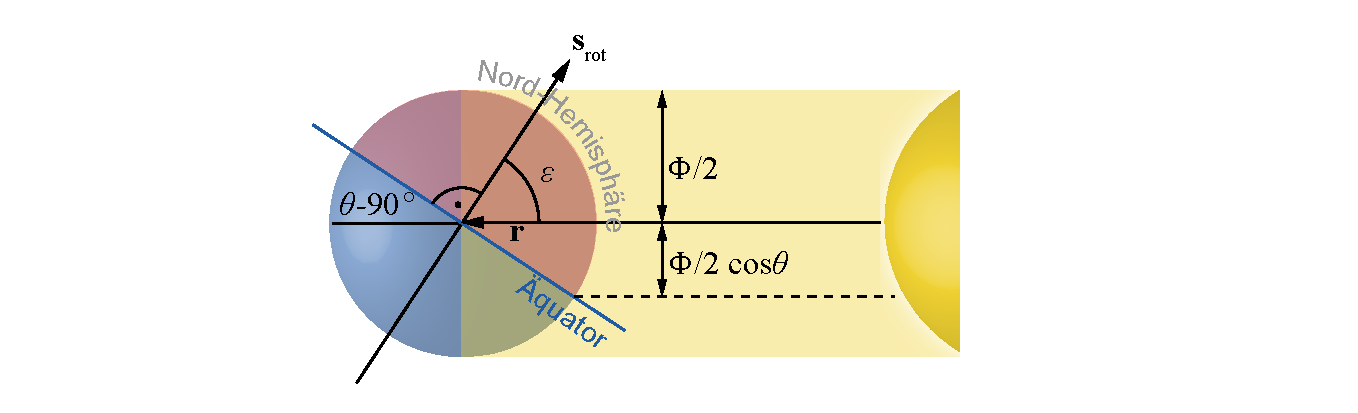
\includegraphics[width=\textwidth]{Erdbahn_im_Jahr_lsg3b.pdf}%
	\caption{Energieeintrag auf die Erde zur Sommersonnenwende}%
	\label{abb:hm_erdbahn_lsg_2}%
	\end{figure}
Der Sonnenlichtstrom $\Phi$ \anf{sieht} die Hemisph�ren unter einem Winkel $\theta$, der sich aus
	\begin{align*}
		\cos\theta(t) &= \frac{\vec{r}(\upsilon)\,\vec{s}_{\text{rot},\earth}}{\abs{\vec{r}(\upsilon)\,\vec{s}_{\text{rot},\earth}}} \nonumber\\
		              &= \lk \begin{matrix} \cos\upsilon(t) \\ \sin\upsilon(t) \\ 0 \end{matrix} \rk\,\lk \begin{matrix} \sin\epsilon \cos\alpha \\ \sin\epsilon\sin\alpha \\ \cos\epsilon \end{matrix} \rk  \\
									&= \sin\epsilon \lek \cos\alpha\cos\upsilon(t) + \sin\alpha\sin\upsilon(t)\rek \nonumber\\
									&= \sin\epsilon\,\cos\lek\upsilon(t)-\alpha\rek ~~ \nonumber
	\end{align*}
ergibt.
Die Sonneneinstrahlung trifft also je nach Jahreszeit auf unterschiedlich gro�e Teilfl�chen der jeweiligen Hemisph�re, der \anf{homogene} Strahlungsstrom verteilt $\Phi$ sich (wie im Bild zur Sommersonnenwende dargestellt) im Nordsommer auf die die Nord-Hemisph�re nach $(1\!+\!\cos\theta)/2$ und auf die S�d-Hemisph�re nach $(1\!-\!\cos\theta)/2$.
Wir berechnen jetzt den Energieeintrag pro "`Halbjahr"' und Hemisph�re und erhalten:
	\begin{align}
		H_\text{N,Sommer}&= C_\text{H}\,\frac{1}{\sqrt{a(1-e^2)}} \int\limits_{\alpha+\pi/2}^{\alpha+3\pi/2} \frac{\lek 1 + \sin\epsilon\cos(\upsilon-\alpha)\rek}{2}\, \D\upsilon \nonumber\\
		&= \frac{1}{2}\,C_\text{H}\,\frac{1}{\sqrt{a(1-e^2)}} \lek \pi-\sin\epsilon\sin(\upsilon-\alpha)\rek_{\alpha+\pi/2}^{\alpha+3\pi/2} \nonumber\\
		&= \frac{1}{2}\,C_\text{H}\,\frac{1}{\sqrt{a(1-e^2)}} (\pi+2\sin\epsilon) ~~.\label{eq:hm_erdbahn_lsg_10}
	\end{align}
	Eine analoge Beziehung erh�lt man f�r den Winter mit 
		\[H_\text{N,Winter} = \frac{C_\text{H}}{2}\,\frac{1}{\sqrt{a(1-e^2)}}\,(\pi-2\sin\epsilon) ~~,
	\]
woraus folgt:
\begin{equation}
\frac{\Delta H_\text{N}}{H_\text{ges}} = \frac{H_\text{N,Sommer} - H_\text{N,Winter}}{H_\text{ges}} = \frac{2\sin\epsilon}{\pi} ~~.\label{eq:hm_erdbahn_lsg_11}
\end{equation}
	
	Mit \eqref{eq:hm_erdbahn_lsg_10} und \eqref{eq:hm_erdbahn_lsg_6} k�nnen wir den durchschnittlichen Energieeintrag pro Zeit (also die empfangene Strahlungsleistung) in der n�rdlichen Hemisph�re f�r das Sommerhalbjahr berechnen:
	\begin{align}
		\frac{H_\text{N,Sommer}}{T_\text{Sommer}} &= P_\text{N,Sommer} \nonumber\\
		&= \frac{C_\text{H}\sqrt{\mu_\text{G}}(\pi+2\sin\epsilon)}{2\sqrt{a(1-e^2)}\, a^{3/2} \lek \pi+4e\cos\alpha-\frac{2e^3}{3}\cos(3\alpha)\rek} \nonumber\\
		&= \frac{P_\text{\astrosun}}{2}\,\lk\frac{R_\text{\earth}^2\sqrt{\mu_\text{G}}}{4\sqrt{\mu_\text{G}}\,a^2 \sqrt{1-e^2}}\rk \,\lk\frac{\pi+2\sin\epsilon}{\pi+4e\cos\alpha-\underbrace{\killA{\frac{2}{3}e^3\cos(3\alpha)}}_{\approx 0}}\rk \nonumber\\
		&\approx \frac{P_\text{\astrosun}}{8}\,\lk\frac{R_\text{\earth}^2}{a^2 \sqrt{1-e^2}}\rk \,\lk\frac{\pi+2\sin\epsilon}{\pi+4e\cos\alpha}\rk ~~.\label{eq:hm_erdbahn_lsg_12}
	\end{align}
	Wir k�nnen uns nun die tats�chlichen Werte und deren zeitliche Entwicklung anschauen.
        Wir finden dazu in den Tabellen \ref{tab:hm_bahnparameter} und \ref{tab:hm_zeitl_aenderung_bahnparameter_lin}
	\begin{align*}
		e &= 0.016709 - 3804\cdot 10^{-8}\,t ~~, \\
		\epsilon &= 23.4392911\degree + 46.8150''\,t =  23.4392911\degree + \frac{46.8150\degree}{3600} \,t ~~.
	\end{align*}
	Hier wird $t$ in Julianischen Jahrhunderten seit $J\,2000$ angegeben.
        F�r $\alpha$ k�nnen wir vereinfachend eine gleichm��ige Perihelpr�zession annehmen:
	\begin{equation*}
	\alpha(t) = \alpha_0 + 1.7192\degree \,t \approx -12.5\degree + 1.7192\degree \,t 
	\end{equation*}
	wobei wir die $1.7192\degree$ bereits als Ergebnis der Perihelverschiebung bzw. der unterschiedlichen L�ngen der tropischen und anomalistischen Jahre kennengelernt hatten.
	
	\begin{figure}[H]
	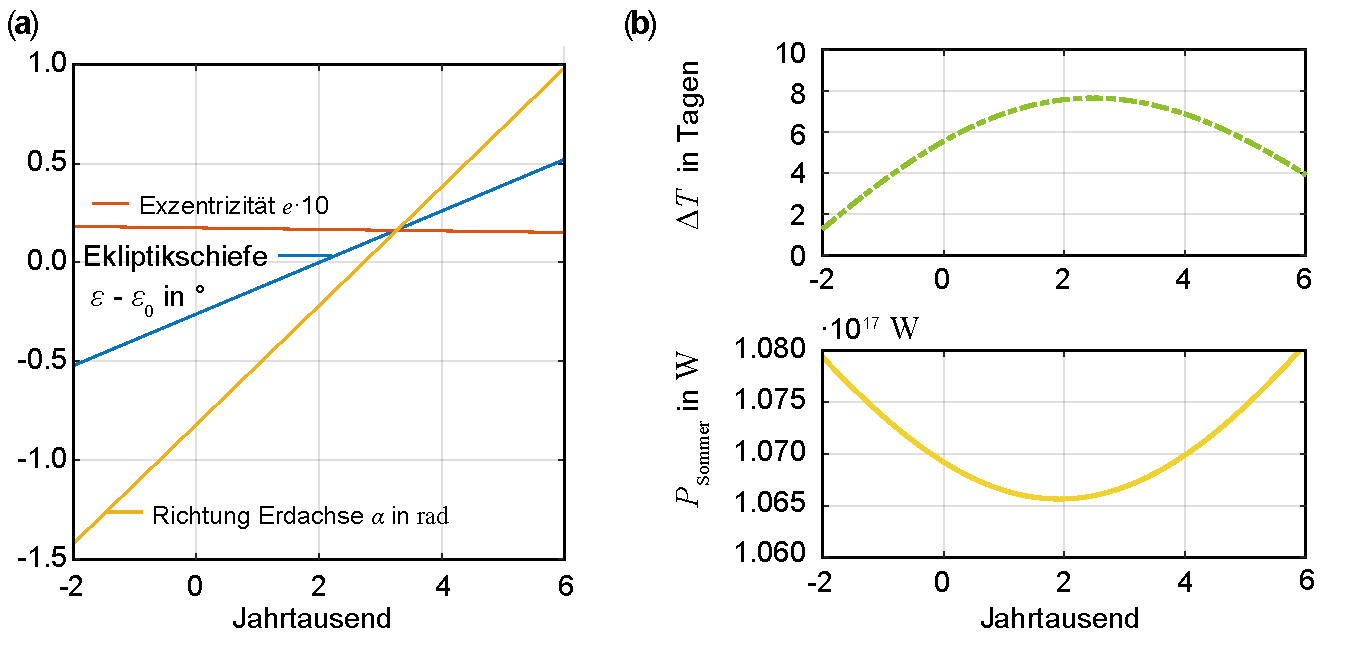
\includegraphics[width=\textwidth]{Erdbahn_im_Jahr_lsg_low.pdf}%
	\caption{Ver�nderung der zeitlichen Dauer der Jahreszeiten.}%
	\label{abb:hm_erdbahn_lsg_3}%
	\end{figure}
	
	In der \figref{hm_erdbahn_lsg_3} finden wir die Ver�nderung der zeitlichen Dauer der Jahreszeiten und auch den sich ver�ndernden  Energieeintrag f�r die Nord-Hemisph�re.
        Wir erkennen, dass wir uns im Moment in einer Trendwende befinden.
        Unser Sommerhalbjahr wird k�rzer werden.
        Gleichzeitig wird der mittlere Energieeintrag pro Halbjahr steigen.
        F�r langfristige Klimaeffekte kann man aber die Formel f�r $e$, $\epsilon$ und $\alpha$ nur bedingt benutzen, sondern muss Parametergleichungen als Funktion von $t$ finden, die einen Zeitraum von mehreren 100000 Jahren beschreiben \cite{Embacher2009}.
\end{enumerate}
\medskip
\end{sol} 
\textcolor{blue} {$\rightarrow$ zur} \probref{hm_erdbahn_im_jahr}.\\
\noindent\rule[1ex]{\textwidth}{0.5pt} \newpage

%-----------------------------------------------------------------------------------------------------------

\begin{sol}{prob:hm_refrak_optik}\label{lsg:hm_refrak_optik} %�bung11
\textbf{Refraktion -- ein Ausflug in die Optik} \\ \\
Wir beginnen mit dem planparallelen Modell (\figref{hm_refr_kugelschale_copy}).

\begin{figure}[H]
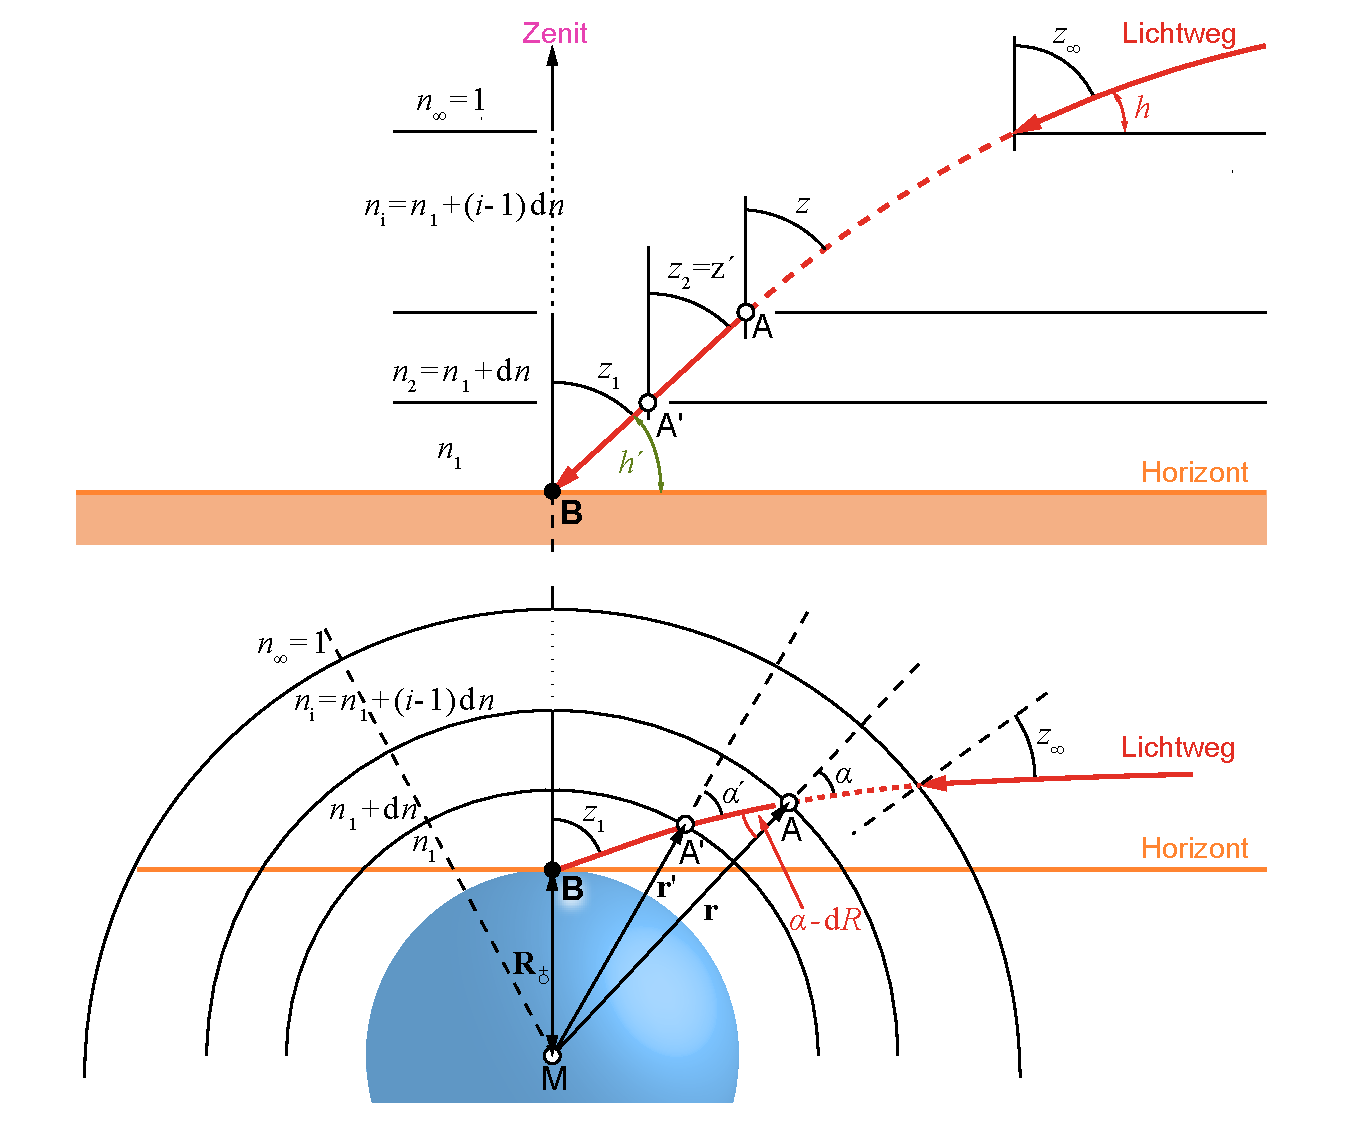
\includegraphics[width=\textwidth]{Refraktion0102.pdf}%
\caption[Planparalleles und Kugelschalen-Schichtenmodell.]{Planparalleles und Kugelschalen-Schichtenmodell zur Berechnung der Refraktion.
F�r die Winkel im $\bigtriangleup\mathrm{A}'\mathrm{MA}$ gilt: $\angle\mathrm{MA}'\mathrm{A}=180\degree-\alpha'$ und $\angle\mathrm{A}'\mathrm{MA}=\alpha-\D R$.}%
\label{abb:hm_refr_kugelschale_copy}%
\end{figure}
F�r die einzelnen Schichten mit unterschiedlichen Brechungsindizes $n_i$ k�nnen wir das Brechungsgesetz wie folgt aufschreiben:
\begin{equation}
n_1\,\sin z_1\,=\, n_2 \,\sin z_2\,=\,n_i\,\sin n_i\,=\,n_\infty\,\sin z_\infty ~~. \label{eq:hm_brechges_lsg12}
\end{equation}
Mit $z_\infty\!=\! [(90\degree - h]$,\, $z_1\!=\!90\degree - h'$,\, $n_\infty\!=\!1$ und der Definition $h\!=\!1h'-R$ folgt daraus
\begin{equation}
n_1\,\sin z_1 = \sin [(90\degree -h') + R] ~~. \label{eq:hm_R_lsg12a}
\end{equation}
Wie nehmen nun an, dass $R$ klein ist, was bei kleinen $z_\infty$ sicherlich gegeben ist und bekommen
\begin{align}
	n_1\,\sin z_1 &= \sin(90\degree - h') \, \cos R + \sin R \cos(90\degree - h')\, \nonumber \\
								& \approx \sin(90\degree - h') + R \cos(90\degree - h') = \sin z_1 + R \cos z_1 \nonumber \\
	\rightarrow ~~~~R &= (n_1 - 1)\,\tan z_1 ~~.  \label{eq:hm_R_lsg12b}
\end{align}
Die Refraktion\footnote{Ungl�cklicherweise bezeichnet man die Refraktion mit $R$, was oft zu Verwechslungen mit Radien und Abmessungen f�hrt. Da in der Literatur und insbesondere in Tabellen aber $R$ benutzt wird, halten wir uns ebenfalls an die Konvention.} $R$ ist also gegeben durch die im Allgemeinen unbekannte Brechzahl am Boden.
Man kann f�r Normalbedingungen und ein ideales Gas annehmen, dass die Brechzahl gem�� folgender Beziehung von der Dichte $\rho_\text{L}$ abh�ngt:
\begin{equation}
\frac{n^2-1}{n^2+2} \propto \rho_\text{L} = \frac{\bar{m}_\text{L} p_\text{L}}{R_0\,T} \label{eq:hm_brechzahl_von_dichte_lsg12}~~,
\end{equation}
worin $p_\text{L}$ der Luftdruck, $R_0\!=\! 8.31\!\cdot\! 10^3\:\text{J/(kmol\,K)}$ die Gaskonstante und $T$ die Temperatur ist.
Wir nehmen Normalbedingungen an, also $p_0\!=\! 101.325\:$kPa und $T_0\!=\! 293\:$K.
$\bar{m}_\text{L}\!\approx\! 28.95\:$kg/kmol ist das mittlere Molek�lgewicht des idealen Gases.
Aus \eqref{eq:hm_brechzahl_von_dichte_lsg12} kann man f�r $n\!\approx\!1$ schreiben:
\begin{equation}
\frac{(n+1)(n-1)}{n^2+2} \approx \frac{2}{3}\,(n-1) \propto \rho_\text{L} ~~.\label{eq:hm_glg4_lsg12}
\end{equation}
Setzt man \eqref{eq:hm_brechzahl_von_dichte_lsg12} und \eqref{eq:hm_glg4_lsg12} f�r verschiedene Temperaturen und Dr�cke ins Verh�ltnis, erh�lt man
\begin{align}
	n_1 - 1 &\approx (n_{10} - 1)\,\frac{p}{p_0}\,\frac{T_0}{T} = (n_{10} - 1)\, 2.6947\,\frac{p}{T} \nonumber\\
\Rightarrow R &= (n_{10}-1)\, 2.6947\,\frac{p}{T}\,\tan(90\degree - h') ~~.\label{eq:hm_glg5_lsg12}
\end{align}
Diese Beziehung f�r $R$ gilt nur f�r kleine $z_1$ oder gr��ere H�hen $h$, also nicht f�r den Fall der Berechnung des Sonnenaufgangs.
Wir wollen deshalb die Refraktion $R$ nach dem Kugelschalenmodell in \figref{hm_refr_kugelschale_copy}b berechnen und k�nnen hier das Brechungsgesetz f�r verschiedene Schichten wie folgt aufschreiben (Man betrachte Punkt A in \figref{hm_refr_kugelschale_copy}b.):
\begin{equation}
(n+ \D n)\,\sin(\alpha-\D R) = n\,\sin\alpha ~~. \label{eq:hm_glg6_lsg12}
\end{equation}
Wiederum ist $\D R$ eine kleine Gr��e, so dass aus \eqref{eq:hm_glg6_lsg12} gleich folgt:
\begin{align}
	(n+\D n)[\sin\alpha \underbrace{\cos(\D R)}_{\approx 1} - \cos\alpha \underbrace{\sin(\D R)}_{=\D R}] &= n\,\sin\alpha \nonumber\\
	\killA{n\,\sin\alpha} + \D n\,\sin\alpha - n\,\cos\alpha\,\D R &= \killA{n\,\sin\alpha} \nonumber\\
	\Rightarrow \D R &= \frac{\D n}{n}\,\tan\alpha ~~. \label{eq:hm_glg7_lsg12}
\end{align}
Wir ersetzen nun $\tan\alpha$ und benutzen dazu den Sinussatz im Dreieck $\bigtriangleup\text{MA'A}$:
\begin{equation}
\frac{\sin\alpha'}{r} = \frac{\sin(\alpha-\D R)}{r'} ~~. \label{eq:hm_glg8_lsg12}
\end{equation}
Kombinieren wir \eqref{eq:hm_glg6_lsg12} und \eqref{eq:hm_glg8_lsg12} erhalten wir durch Einsetzen von $\sin(\alpha-\D R)$
\begin{equation*}
r'(n + \D n)\,\sin\alpha' = rn\,\sin\alpha ~~.
\end{equation*}
Diese Beziehung gilt analog zu \eqref{eq:hm_brechges_lsg12} f�r alle Schichten.
Deshalb k�nnen wir schreiben:
\begin{equation}
rn(r)\,\sin\alpha = R_\text{\earth} n_1\,\sin z_1
\label{eq:hm_glg9_lsg12}~~.
\end{equation}
Wir benutzen jetzt noch die trigonometrische Beziehung $\tan\alpha = \sin\alpha/\sqrt{1-\sin^2\alpha}$ und k�nnen damit \eqref{eq:hm_glg7_lsg12} umformen zu
\begin{equation}
R(z_1) = \int \D R = \int\limits_{n=1}^{n=n_1} \frac{1}{n}\,\frac{A \sin z_1}{\sqrt{1-A^2\sin^2 z_1}} \,\D n \label{eq:hm_glg10_lsg12}
\end{equation}
mit 
	\[	A(n)\!=\frac{\!R_\text{\earth} n_1}{r n(r)} ~. 
	\]
Die Gleichung \eqref{eq:hm_glg10_lsg12} nennt man das Refraktionsintegral.\index{Refraktionsintegral}
Will man dieses auswerten, so muss man Annahmen f�r $n(r)$ bzw. $\rho_\text{L}(r)$ machen, die wiederum von $T(r)$ und $p(r)$ abh�ngen.
Im Allgemeinen wird das Integral numerisch gel�st.
Man kann dann auch beliebige Schichtmodelle annehmen und $ R$ �ber
\begin{equation*}
R = \sum_{i=1}^{i=N} \tan\alpha_i\,\lk\frac{n_{i+1} - n_i}{n_i}\rk
\end{equation*}
mit $\alpha_1\!=\! z_1\!=\! z_\text{schein}$ berechnen. 
Interessant ist noch, dass bereits Newton auf Basis seiner Korpuskulartheorie des Lichtes die Berechnung der Refraktion vornahm und diese als eine der kompliziertesten Aufgaben seines Lebens bezeichnete \cite{Nauenberg2017}. Er berechnete die Trajektorie des Lichtteilchens, welches durch die Brechung unter einer \emph{Zentralkraft} der Form
\begin{equation*}
\vec{F} = n\,\frac{\D n}{\D r} \frac{\vec{r}}{r}
\end{equation*}
steht.
Mit den Methoden, die wir in \kapitel{hm_bewegungsgl} dargestellt haben, insbesondere die Benutzung der Drehimpulserhaltung, kann man die Trajektorie des Teilchens als 
\begin{equation*}
z(r) = \bigintss\limits_{r_1 = R_\text{\earth}}^{r} \frac{\sin z_1}{r' \sqrt{\lk \frac{n(r') r'}{n_1 R_\text{\earth}} \rk^2 - \sin^2 z_1}} \D r'
\end{equation*}
und die Refraktion als
\begin{equation*}
R(z_1) = z_1 - z(r\rightarrow\infty) \equiv R(z') = z' - z 
\end{equation*}
schreiben \cite{Nauenberg2017}.
Wir wollen noch die Formulierung des Refraktionsintegrals f�r eine einfache Abh�ngigkeit der Brechungsindizes von der H�he angeben, der durch eine exponentielle Abnahme der Dichte nach
\begin{align*}
	\rho(r') = \rho(R_\text{\earth})\,\E^{-h/H} = \rho_0\,\E^{-h/H} ~~\text{mit} ~~ h = r - R_\text{\earth}
\end{align*}
nach folgender Formel 
\begin{align*}
	n(r') -1 = \kappa \,\frac{\rho(r')}{\rho(R_\text{\earth})} 
\end{align*}
gegeben ist, worin $\kappa$ und $H$ Konstanten der Erdatmosph�re sind.
In das Refraktionsintegral \eqref{eq:hm_glg10_lsg12} eingesetzt, ergibt das 
\begin{equation}
R(z_1) = \kappa \bigintss\limits_{0}^{\infty} \frac{\E^{-x}\,\sin z_1}{\lk 1+\kappa \E^{-x}\rk\,\sqrt{\lek \lk 1+\kappa \E^{-x} \rk \lk 1 + \frac{Hx}{R_\text{\earth}} \rk / \lk 1+\kappa\rk \rek^2 - \sin^2 z_1}} \:\D x ~~, \label{lsg:hm_refraktionsintegral2}
\end{equation}
welches wir in \mlhmref{Refraktion.m} f�r verschiedene Parameter $\kappa, H$ ausgewertet haben.
Als Parameter f�r einen relativ guten Fit an die Formel \eqref{eq:hm_Normalrefraktion1} haben wir aus der ISA-Tabelle \cite{ISA1976} die Werte $\kappa\!=\! 0.000316$ und $H\!=\! 9.87 $ km gew�hlt.

\begin{figure}[H]
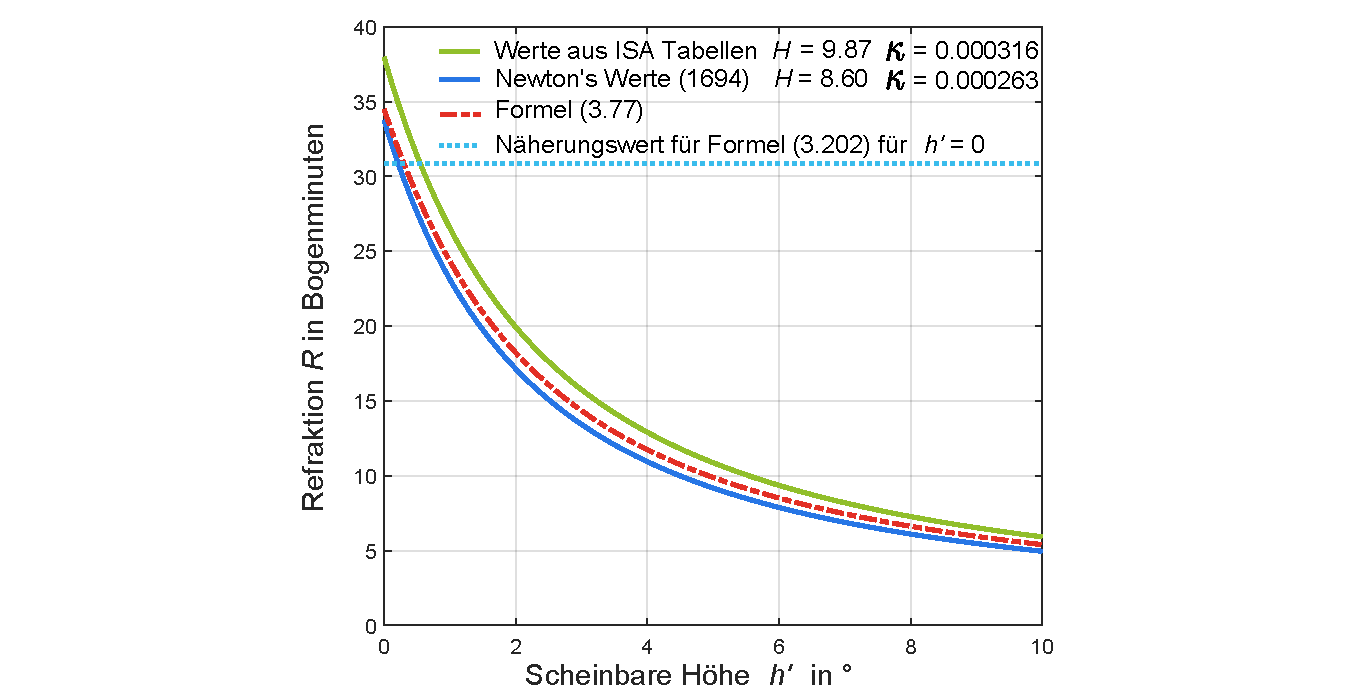
\includegraphics[width= \textwidth]{Refraktion12.pdf}%
\caption[Berechnete Refraktionskurven nach dem Kugelschalen-Schichtenmodell.]{Berechnete Refraktionskurven nach dem Kugelschalen-Schichtenmodell \eqref{lsg:hm_refraktionsintegral2} und Vergleich mit \eqref{eq:hm_relations2} sowie den Berechnungen von Newton \cite{Nauenberg2017}.}%
\label{abb:hm_Refraktion12}%
\end{figure}
\medskip \end{sol}
\textcolor{blue} {$\rightarrow$ zur} \probref{hm_refrak_optik}.\\
\noindent\rule[1ex]{\textwidth}{0.5pt} \newpage


\begin{sol}{prob:hm_abflachung_sonne} \label{lsg:hm_abflachung_sonne} %�bung12
\textbf{Abflachung der Sonne beim Untergang} \\

\begin{figure}[H]
\includegraphics[width=1.0\textwidth]{AbflachungSonne.pdf}%
\caption[Berechnung der Abflachung der Sonne bei Sonnenuntergang.]{Berechnete Form und H�he der Sonne mit (links) und ohne Refraktion (rechts). Bildmitte: Aufnahme Sonnenuntergang auf Hawaii (Bernd Geh am 10.11.2016 um 17:42:32) und dazu berechnete Form und Position.}%
\label{abb:hm_AbflachungSonne}%
\end{figure}

Wir benutzen zur L�sung die Refraktionsformel Formel \eqref{eq:hm_Normalrefraktion2}.
im Bild links sind die \anf{abgeflachten} Sonnen in der scheinbaren H�he zu sehen und rechts im Bild in gleicher Farbumrandung in astrometrische H�he und in der nicht durch Refraktion beeinflussten Form der \anf{Sonnenscheibe}.
In der Mitte ist ein auf Hawaii von Bernd Geh aufgenommenes Bild der untergehenden Sonne gefittet.
Wir verweisen auf \mlhmref{AbflachungSonne.m} und bedanken uns bei Bernd Geh (\href{http://www.bgeh-photography.com/Home.html}{http://www.bgeh-photography.com/Home.html}) f�r die Bereitstellung des Bildes und die Anregungen zur �bung.\\
\medskip \end{sol}
\textcolor{blue} {$\rightarrow$ zur} \probref{hm_abflachung_sonne}.\\
\noindent\rule[1ex]{\textwidth}{0.5pt} \newpage

\begin{sol}{prob:hm_tageslauf_sonne} \label{lsg:hm_tageslauf_sonne} %�bung13
\textbf{Tageslauf der Sonne} \\ \\
Wir verweisen auf das \mscr~\mlhmref{TageslaufSonne.m}. \\
\medskip \end{sol}
\textcolor{blue} {$\rightarrow$ zur} \probref{hm_tageslauf_sonne}.\\
\noindent\rule[1ex]{\textwidth}{0.5pt} \newpage

\begin{sol}{prob:hm_sonnenaufg_nyc}\label{lsg:hm_sonnenaufg_nyc} %�bung14
\textbf{Sonnenaufgang in New York City} \\ \\
Basierend auf \figref{hm_nyc_lsg} berechnen wir zun�chst aus der geographischen Breite $\varphi= 40.7\degree$ von New York City (NYC) den Radius des Erdellipsoids an dieser Stelle \cite{Meeus1998}:
\begin{align*}
	r_\text{NYC} &= \lek 0.9983271 + 0.0016764 \cos(2\varphi) - 0.0000035 \cos(4\varphi)\rek\, 6378137\:\text{m} \\
	&= 6369087\:\text{m}~.\\
\end{align*}

\begin{figure}[H]

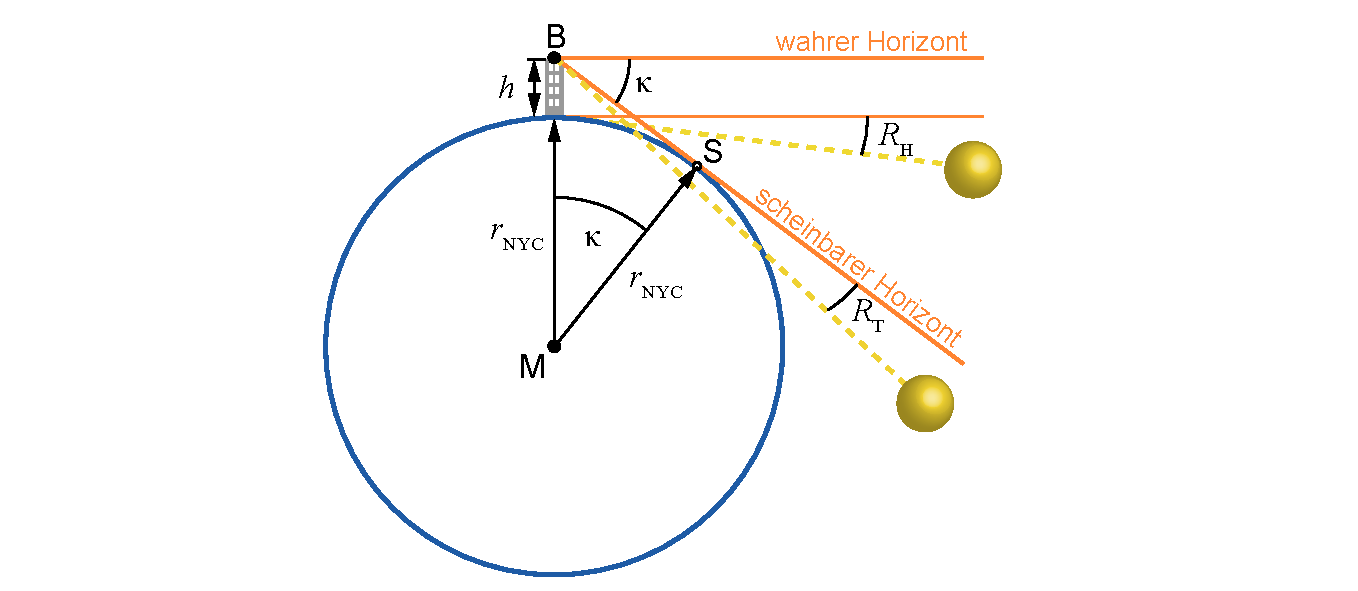
\includegraphics[width=\textwidth]{SonnenaufgangNYC.pdf}%
\caption{Geometrie zum Sonnenaufgang in New York City}%
\label{abb:hm_nyc_lsg}%
\end{figure}

Die H�he $h$ des One World Trade Centers betr�gt $531\:$m.
Daraus ergibt sich der Winkel $\kappa$ aus \figref{hm_nyc_lsg} �ber.
Es gilt weiterhin
\begin{align*}
	(r_\text{NYC} + h)^2 &= \overline{\text{BS}}^2 + r_\text{NYC}^2 \\
	\rightarrow \overline{\text{BS}} &\approx \sqrt{2\,h\,r_\text{NYC}} ~~\text{f�r}~~h\ll r_\text{NYC}~~.
\end{align*}
Es ergibt sich f�r kleine Winkel $\kappa$:
\begin{equation}
\tan \kappa \approx \sin \kappa = \frac{\overline{\text{BS}}}{r_\text{NYC}} = \sqrt{\frac{2h}{r_\text{NYC}}}~~,
\end{equation}
woraus $\kappa = 0.73981$ folgt.
Wir sehen ferner aus der Abbildung, dass ohne Ber�cksichtigung der Refraktion, der Sonnenaufgang um eine bestimmte Zeitdauer $\Delta t$ fr�her stattfindet.
$\Delta t$ entspricht der Zeit, die die Sonne br�uchte, um die H�he $h$ zu durchlaufen.
Wenn wir noch ber�cksichtigen, dass die Refraktion $R_\text{T}$ etwas gr��er ist als $R_\text{H}$,\footnote{Das Licht durchl�uft dichtere Luftschichten deutlich langsamer.} dann k�nnen wir f�r die Tagbogenverl�ngerung mit \eqref{eq:hm_tagbogverl} und $\delta\!= \epsilon\!\,$ folgendes aufschreiben:
\begin{align*}
	\Delta\tau_\text{B,H} &= -\frac{h_\text{r,H}}{\sqrt{\cos^2\delta - \sin^2\varphi}} = \frac{-16' - R_\text{H}}{\sqrt{\cos^2\delta - \sin^2\varphi}} ~~,\\
	\Delta \tau_\text{B,T} &= -\frac{h_\text{r,T}}{\sqrt{\cos^2\delta - \sin^2\varphi}} = \frac{-\kappa-16' - R_\text{T}}{\sqrt{\cos^2\delta - \sin^2\varphi}} ~~.
\end{align*}
Aus \eqref{eq:hm_Normalrefraktion1} finden wir zun�chst $R_\text{H} \!=\!R(0)\!\approx\! 34'$ und $R_\text{T} \!=\!R(-\kappa)\!\approx\! 45'$ und somit
\begin{align}
	\Delta t &= \Delta\tau_\text{B,1} - \Delta\tau_\text{B,0} \\
	        &= -\frac{(R_\text{T} - R_\text{H})+\kappa}{\sqrt{\cos^2 \delta - \sin^2 \varphi}} \\
					&\approx 5\:\text{min} ~ 45\:\text{s}~~.
\end{align}
Der Beobachter auf dem One World Trade Center sieht also die Sonne fast $6\:$min fr�her als jener auf Ellis Island.
Es lohnt sich also seinen Morgenkaffee auf dem One WTC zu trinken.\\
\medskip \end{sol}
\textcolor{blue} {$\rightarrow$ zur} \probref{hm_sonnenaufg_nyc}.\\
\noindent\rule[1ex]{\textwidth}{0.5pt} \newpage


%-----------------------------------------------------------------------------------------------------------

\begin{sol}{prob:hm_analytic_sunrise}\label{lsg:hm_analytic_sunrise} %�bung15
\textbf{Analytische Formel f�r den Sonnenaufgang und Sonnenuntergang} \\ \\
Wir folgen hier der Darstellung in \cite{Reinsch2003} und starten von der Beziehung f�r die astronomische H�he als Funktion des Stundenwinkels \eqref{eq:hm_Alt-Az-Koord}
\begin{equation*}
\sin h = \cos\delta \cos\tau \cos\varphi + \sin\delta \sin\varphi ~~.
\end{equation*}
Wir ersetzen die Deklination $\delta$ durch die geozentrisch-ekliptikale Koordinate $\lambda$ nach \eqref{eq:hm_drehung_x_achse_linear2} und erhalten mit $\beta\!=\!0$ und $\tau\!=\!\Theta-\alpha$ gem�� \eqref{eq:hm_std_winkel_tau} f�r die Sonne
\begin{align}
\sin h =&\, \underbrace{\cos\delta \cos\alpha}_{=\cos\lambda} \cos\Theta \cos\varphi + \underbrace{\cos\delta \sin\alpha}_{\sin\lambda \cos\epsilon} \sin\Theta \cos\varphi\, + \underbrace{\sin\delta}_{\sin\lambda \sin\epsilon} \sin\varphi \nonumber\\
			 =&\, \cos\lambda \cos\Theta \cos\varphi + \sin\lambda\cos\epsilon\sin\Theta\cos\varphi + \underbrace{\sin\lambda \sin\epsilon \sin\varphi}_{\equiv\text{T}_\text{II}} ~~. \label{eq:hm_sa_su_lsg1}
\end{align}
Die Aufgabe besteht nun darin, $\Theta(h\!=\!0)$ bzw. $\tau(h\!=\!0)$ f�r die Tage eines Jahres zu bestimmen.
Wir wollen dabei vereinfachend f�r die Sternzeit $\Theta$ annehmen, dass
\begin{equation}
\Theta = \frac{2\pi}{\text{d}_\diamond}\, t = \frac{2\pi}{86164\:\text{s}}\, t ~~. \label{eq:hm_sa_su_lsg2a}
\end{equation}
F�r die Weltzeit UT schreiben wir 
\begin{equation}
\hat{\Theta} = \frac{2\pi}{\text{d}_\text{\astrosun}}\, t = \frac{2\pi}{86400\:\text{s}}\, t ~~. \label{eq:hm_sa_su_lsg2b}
\end{equation}
Da wir besser die Uhrzeit und nicht die Sternzeit des Sonnenaufgangs bestimmen wollen, formen wir dies um zu
\begin{equation*}
\Delta (t) = \Theta - \hat{\Theta} ~~\text{bzw.}~~ \Theta = \hat{\Theta}+\Delta
\end{equation*}
und setzen diese Beziehung in \eqref{eq:hm_sa_su_lsg1} ein.
$\Delta (t)$ beschreibt im Prinzip das \anf{Auseinanderlaufen} von Sternzeit und Weltzeit, was exakt durch \eqref{eq:hm_UT_3} gegeben ist.
F�r unsere Absch�tzung des Sonnenaufgangs gen�gt aber der einfache Ansatz nach \eqref{eq:hm_sa_su_lsg2a} und \eqref{eq:hm_sa_su_lsg2b}.
Wir bekommen also
\begin{equation*}
\sin h = \underbrace{\cos\lambda \cos(\hat{\Theta}+\Delta) \cos\varphi + \sin\lambda \cos\epsilon \sin(\hat{\Theta}+\Delta) \cos\varphi}_{\equiv \text{T}_\text{I} = X \cos(\hat{\Theta}+\xi)\cos\varphi} + \text{T}_\text{II} ~~,
\end{equation*}
was eine algebraische Umformung unter Nutzung der Additionstheoreme ist. Mit den Termen
\begin{equation*}
X = \sqrt{\lk \cos\epsilon \sin\lambda \sin\Delta + \cos\lambda \cos\Delta \rk^2 + \lk \cos\epsilon \sin\lambda \cos\Delta - \cos\lambda \sin\Delta\rk^2}
\end{equation*}
und
\begin{equation*}
\xi = -\arctan \lk \frac{\cos\epsilon \sin\lambda \cos\Delta - \cos\lambda \sin\Delta}{\cos\epsilon \sin\lambda \sin\Delta + \cos\lambda \cos\Delta} \rk
\end{equation*}
erhalten wir schlie�lich
\begin{equation}
\sin h = \text{T}_\text{I} + \text{T}_\text{II} = X \cos (\hat{\Theta}+\xi) \cos\varphi + \sin\lambda \sin\epsilon \sin\varphi ~~.\label{eq:hm_sa_su_lsg3}
\end{equation}
Wir m�ssen jetzt eigentlich nur noch \eqref{eq:hm_sa_su_lsg3} nach $\hat{\Theta}$ f�r $h\!=\!0$ l�sen und machen hierzu die folgende N�herungen:
\begin{itemize}
	\item Vernachl�ssigung der Refraktion,
	\item Annahme, dass die ekliptikale L�nge $\lambda$ und $\Delta$ f�r die Dauer eines Tages konstant sind.
\end{itemize}
Wenn man mit \eqref{eq:hm_sa_su_lsg2a} mod $24\:$h bzw. mod $\pi$ nimmt und $h\!=\!0$ aus \eqref{eq:hm_sa_su_lsg3} benutzt, folgt daraus
\begin{equation}
\hat{\Theta}_\text{A,U} = \pm \arccos \lk - \frac{\sin\lambda \sin\epsilon \tan\varphi}{X} \rk - \xi ~~. \label{eq:hm_sa_su_lsg4}
\end{equation}
Dabei gilt das Minuszeichen f�r den Sonnenaufgang und das Pluszeichen f�r den Sonnenuntergang.
Laut unserer Definition der ekliptikalen L�nge ist ja am Fr�hlingspunkt $\lambda\!=\!0$ und die Uhren sind synchron  $\hat{\Theta} = \Theta$.
Es folgt demnach
\begin{equation*}
\hat{\Theta}_\text{A,U}(\vernal) = \underbrace{\tan \Delta(\vernal)}_{0} \pm \arccos (0) = \pm \frac{\pi}{2} = \pm 6\:\text{h} 
\end{equation*}
und damit der Sonnenaufgang als $\text{SA}\!=\!12\:\text{h}-\hat{\Theta}(\vernal) =$ 06:00h UT.
Wir haben mit \eqref{eq:hm_sa_su_lsg4} eine relativ �bersichtliche Formel f�r die Berechnung der Sonnenaufg�nge und Sonnenunterg�nge gefunden. 

\begin{figure}[H]
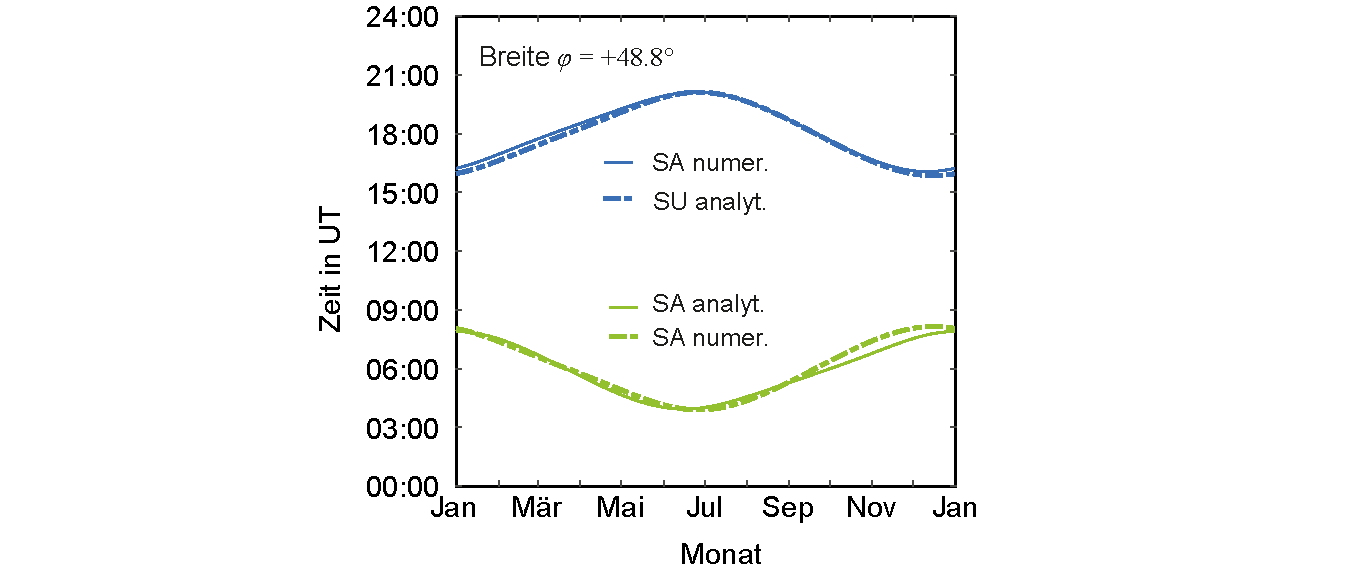
\includegraphics[width=\columnwidth]{Sunrise_lsg.pdf}%
\caption[Analytische und numerische L�sung Sonnenauf- und Sonnenuntergang.]{Analytische und numerische L�sung des Sonnenaufgangs und Sonnenuntergangs.}%
\label{abb:hm_sunrise_lsg}%
\end{figure}

Als Parameter f�r die N�herungsl�sung ben�tigen wir die L�nge des Sternen- und Sonnentags in Sekunden, die geographische Breite $\varphi$, die Ekliptikschiefe $\epsilon$ und die ekliptikale L�nge $\lambda$.
Letztere beschaffen wir uns wieder aus der Mittelpunktsgleichung \eqref{eq:hm_ekl_laenge_bogenmass}, womit in \eqref{eq:hm_sa_su_lsg4} wieder beide Effekte (Ekliptikschiefe und Elliptizit�t der Bahn) ber�cksichtigt worden sind.
In \figref{hm_sunrise_lsg} vergleichen wir die L�sung in \eqref{eq:hm_sa_su_lsg4} mit der numerischen L�sung, die �bereinstimmung ist relativ gut.
Es sei erw�hnt, dass die N�herungsformeln nicht gelten, wenn wir in den Bereich $\abs{\varphi}\!>\!+(90\degree\!-\!\epsilon)$ kommen.
Die analytische Formel wird dar�ber hinaus auch wegen des Verhaltens der $\arccos$-Funktion bei kleinen Argumenten f�r $\abs{\varphi}\!\ll\! \epsilon$ ungenau.
\medskip \end{sol}
\textcolor{blue} {$\rightarrow$ zur} \probref{hm_analytic_sunrise}.\\
\noindent\rule[1ex]{\textwidth}{0.5pt} \newpage


%-----------------------------------------------------------------------------------------------------------

\begin{sol}{prob:hm_VertikalAnalemmaSonnenuhr} \label{lsg:hm_VertikalAnalemmaSonnenuhr} %\�bung16
\textbf{Konstruktion von Sonnenuhren} \\

Konstruktion einer vertikalen und einer analemmatischen Sonnenuhr:
\begin{figure}%
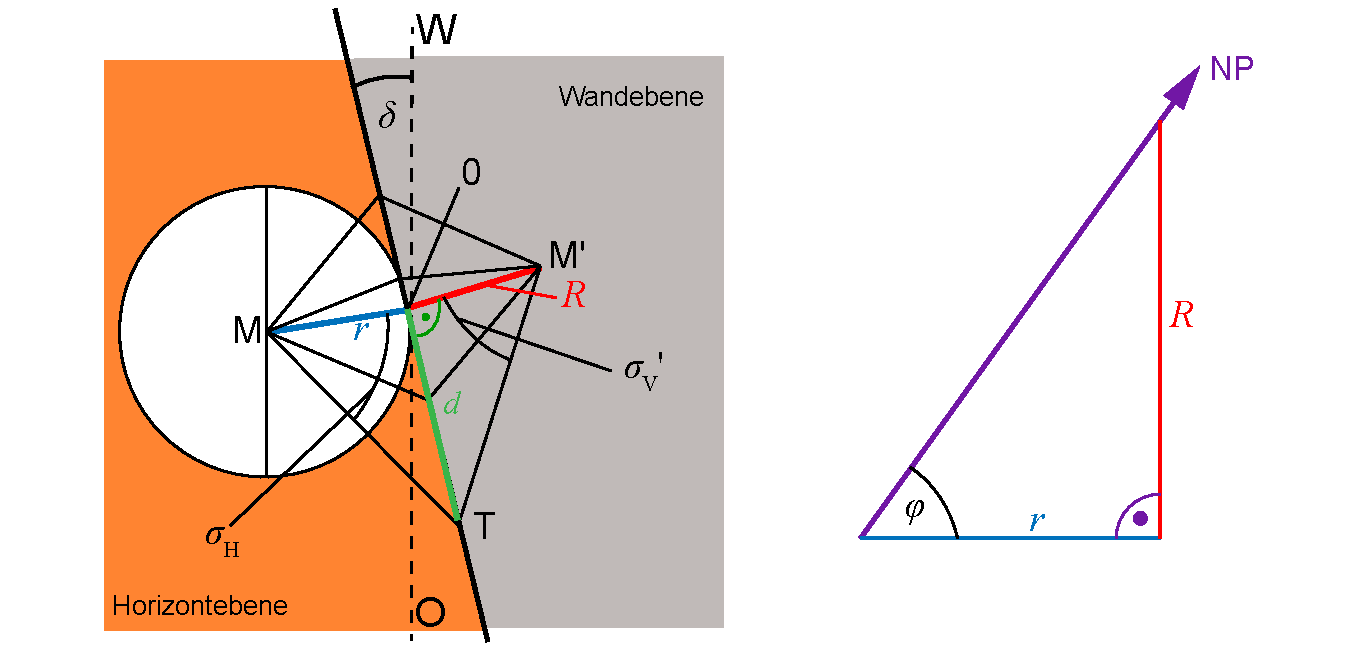
\includegraphics[width=\textwidth]{Sonnenuhr05.pdf}%
\caption[Ausf�hrung und Prinzip der Vertikal-Sonnenuhr.]{Ausf�hrung und Prinzip der Vertikal-Sonnenuhr bei  beliebiger Ausrichtung der Wand.}%
\label{abb:hm_sundial_lsg01}%
\end{figure}

\begin{enumerate}
 \item [a)]  

Wir betrachten zun�chst die Sonnenuhr, die an einer Hauswand angebracht ist, welche unter einem beliebigen Winkel $\delta$ zur Ost-West-Richtung steht.
Der Verdrehwinkel $\delta$ zur Wand sei negativ bei Ausrichtung SW-NO, wie im dargestellten Fall.
Aus \figref{hm_sundial_lsg01} lesen wir folgende Beziehungen ab:
    \begin{align}
        \tan\sigma_v{}' &= \frac{\overline{\text{0T}}}{R} = \frac{d}{R} \label{eq:hm_sundial_lsg01} \\
        \sphericalangle (\text{MT0}) &= 180\degree - (90\degree - \delta) - \sigma_\text{H} = 90\degree - (\sigma_\text{H} -\delta)\,. \label{eq:hm_sundial_lsg01a} 
    \end{align}
    Aus dem Sinussatz f�r das Dreieck $\Delta (\text{MT0})$ folgt:
    \begin{align}
        \frac{\sin\sigma_\text{H}}{d} = \frac{\sin \sphericalangle (\text{MT0})}{r} ~~~~\rightarrow ~~~~ d = r\,\frac{\sin\sigma_\text{H}}{\cos\lk \sigma_\text{H} - \delta \rk} \,. \label{eq:hm_sundial_lsg02}
    \end{align}
    Mit der Beziehung \eqref{eq:hm_sundial02} f�r die Radien $r$ und $R$ \,$ \tan\varphi = R/r$ und mit \eqref{eq:hm_sundial_lsg01} und \eqref{eq:hm_sundial_lsg02} folgt daraus:
    \begin{align}
        \tan\sigma_\text{V}{}' &= \frac{\sin\sigma_\text{H}}{\cos\lk \sigma_\text{H}- \delta\rk}\,\frac{1}{\tan\varphi} ~~~~ \text{mit} ~~~~ \sigma_\text{H} = \arctan \lk\sin\varphi\,\tan\sigma_\text{A} \rk \nonumber \\
				\rightarrow~\sigma_\text{V}{}' &= \arctan\lk \frac{\cos\varphi}{\cos\delta \cot\sigma_\text{A} + \sin\varphi \sin\delta}\rk	\,.
\label{eq:hm_sundial_lsg03}
    \end{align}
    F�r $\delta \to 0$ folgt daraus mit 
    \begin{align*}
        \tan\sigma_\text{V}{}' &= \frac{\sin\sigma_\text{H}}{\cos\sigma_\text{H}}\,\frac{1}{\tan \varphi} = \frac{\sin\varphi}{\tan\varphi}\,\tan\sigma_\text{A} = \cos\varphi\,\tan\sigma_\text{A} \\
    \end{align*}
    die Beziehung f�r die O-W ausgerichtete Wand.
    Die Lineatur f�r eine Sonnenuhr in Oberkochen ($\varphi = 48\degree$ N) und einer Wand die etwa ONO-WSW ausgerichtet ist ($\delta = -22.5\degree$) ist in \figref{hm_sundial_lsg02} zu sehen.\\

\begin{figure}%
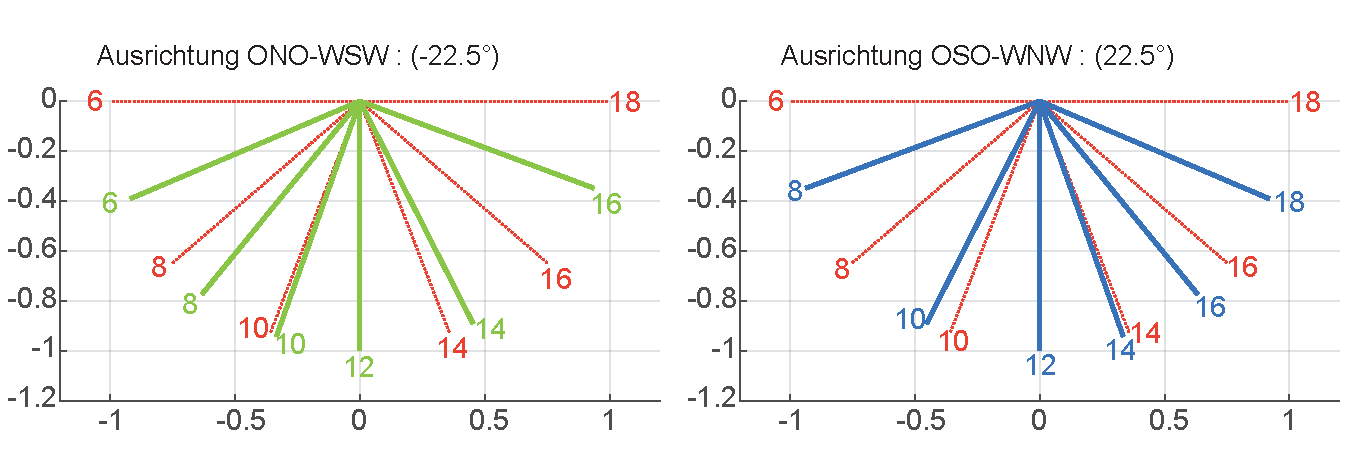
\includegraphics[width=\textwidth]{Wandsonnenuhr.pdf}%
\caption[Lineatur f�r eine Wandsonnenuhr in Oberkochen.]{Lineatur f�r eine Wandsonnenuhr in Oberkochen f�r verschiedene Ausrichtungen. Siehe \mlhmref{Wandsonnenuhr.m}} 
\label{abb:hm_sundial_lsg02}%
\end{figure}

\item [b)]

Nun wollen wir die Lineatur f�r eine analemmatischen Sonnenuhr in der Stadt G�rlitz (Breitengrad $\varphi = 51.2\degree$ und L�ngengrad $\lambda = 15\degree$) berechnen. 
Aus \eqref{eq:hm_sundial06} k�nnen wir die Abbildung $\vec{r}_n$ des Nodus aus der Sonnenrichtung $\vec{s}$ auf dem Ziffernblatt (welches in der Horizontalebene liegt) als Funktion des Datums und der Zeit, m.\,a.\,W.\ als Funktion des Sonnenstandes f�r eine bestimmte geographische Breite berechnen. \\
Wir k�nnen zur Berechnung nat�rlich vorteilhafter weise, die in \kap{hm_naeherungsformeln_sonne} berechneten Beziehungen f�r die H�he $h$ und das Azimut $\mathcal{A}$ der Sonne benutzen. Dann ergeben sich die Linien des Schatten des Nodus f�r einen bestimmten Tag eines Jahres $d_\text{fix}$ durch (wir nehmen die WSW, SSW und die Tag- und Nachtgleichen):
    \begin{align}
        \vec{r}_n (t) &= 
         \begin{pmatrix}
         \cos \lk h\lk t, d_\text{fix}\rk \rk \, \cos \lk \mathcal{A}\lk t,d_\text{fix} \rk\rk \\
         \cos \lk h\lk t, d_\text{fix}\rk \rk \, \sin \lk \mathcal{A}\lk t,d_\text{fix} \rk\rk \\
         0
         \end{pmatrix}\cdot
         \frac{H}{\sin h\lk t,d_\text{fix} \rk}\nonumber \\
          &= H\, 
         \begin{pmatrix}
             \cot\lk h\lk t,d_\text{fix}\rk\rk\,\cos\lk \mathcal{A}\lk t,d_\text{fix}\rk\rk\\
             \cot\lk h\lk t,d_\text{fix}\rk\rk\,\sin\lk \mathcal{A}\lk t,d_\text{fix}\rk\rk\\
             0
         \end{pmatrix} \,.  \label{eq:hm_lsgsundial11}
    \end{align}
    Analog ergibt sich f�r eine feste Uhrzeit $t_\text{fix}$ und die verschiedenen Tage $d$ des Jahres nat�rlich die Form des Analemma. 
    \begin{align}
        \vec{r}_n (d) = H\,
        \begin{pmatrix}
            \cot\lk h\lk t_\text{fix},d\rk \rk \, \cos\lk \mathcal{A}\lk t_\text{fix},d\rk \rk \\
            \cot\lk h\lk t_\text{fix},d\rk \rk \, \sin\lk \mathcal{A}\lk t_\text{fix},d\rk \rk \\
            0
        \end{pmatrix} \,.  \label{eq:hm_lsgsundial12}
    \end{align}
    $d$ steht hier f�r die Tage des Jahres. Die bei den Einzellineaturen nach \eqref{eq:hm_lsgsundial11} und \eqref{eq:hm_lsgsundial12} sind in \figref{hm_sundial_lsg03} zur Lineatur der Sonnenuhr zusammengesetzt.\\
    Eine besonders elegante analemmatische Sonnenuhr ist in Ref \cite{Heierli2019} beschrieben, die sich auch gut wie fast alle Sonnenuhren als Schmuckst�ck eignet. Wir verweisen auch auf die Aalener Sonnenuhr in der Zusatzaufgabe \probref{hm_Aalener_Sonnenuhr}, die in �hnlicher weise wie hier vorgestellt berechnet werden kann.
\end{enumerate}
\begin{figure}%
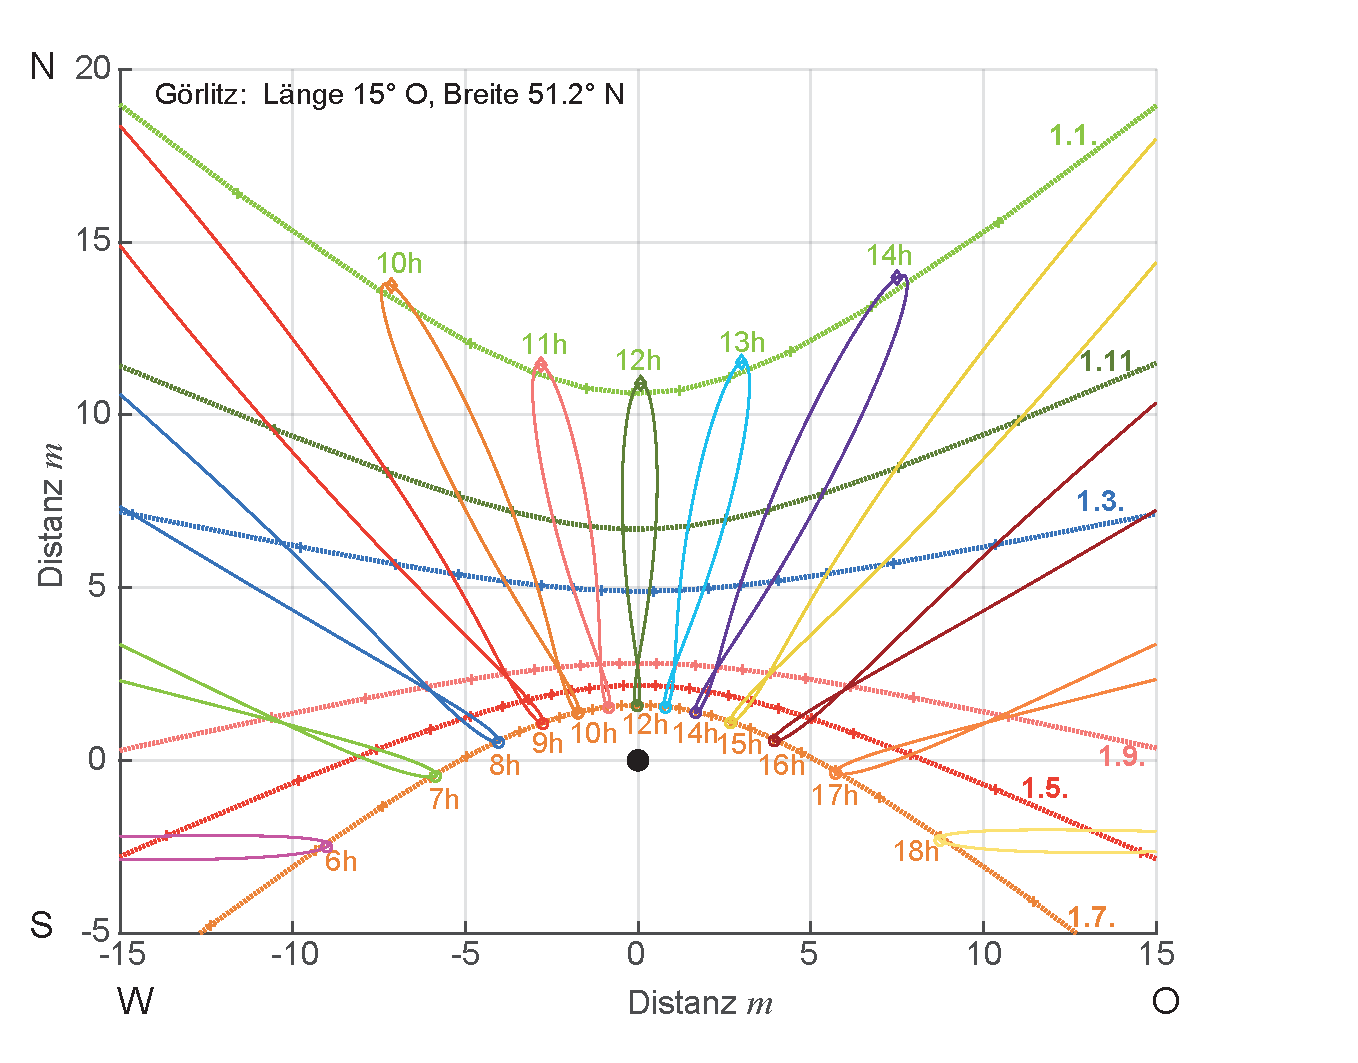
\includegraphics[width=\textwidth]{SonnenuhrAnalem.pdf}%
\caption[Berechnetes Ziffernblatt einer analemmatischen Sonnenuhr f�r G�rlitz.]{Berechnetes Ziffernblatt einer analemmatischen Sonnenuhr f�r G�rlitz. Siehe \mlhmref{SonnenuhrAnalem.m}} %
\label{abb:hm_sundial_lsg03}%
\end{figure}

\medskip \end{sol}
\textcolor{blue} {$\rightarrow$ zur} \probref{hm_VertikalAnalemmaSonnenuhr}.\\
\noindent\rule[1ex]{\textwidth}{0.5pt} \newpage


%-----------------------------------------------------------------------------------------------------------

\begin{sol}{prob:hm_opposition_mars}\label{lsg:hm_opposition_mars} %�bung17
\textbf{Mars-Oppositionen von 2000 bis 2020} \\ \\
Wir berechnen mit Hilfe der Gau�schen Vektoren die Bahnen von Mars und Erde in heliozentrischen Koordinaten und bestimmen die Zeitpunkte, an denen $l_\text{\mars}\!=\!l_\text{\earth}$ ist.
Es ergibt sich dann auch der minimale Abstand $\Delta r$.
Man sieht, dass auf Grund der relativ exzentrischen Bahn des Mars (\figref{hm_mars_opposition_lsg}), die Mars-Oppositionen nahe des Perihels dahingehend ausgezeichnet sind, dass der Mars der Erde besonders nahe kommt.
Wir m�ssen dann noch folgende Parameter berechnen:
\begin{itemize}
	\item Geozentrische Breite des Mars:
	   \begin{equation*}
		  \beta = \arcsin(z_\text{\mars}/\Delta r)
		 \end{equation*}
	\item Deklination des Mars zum Oppositionszeitpunkt \eqref{eq:hm_drehung_x_achse_linear2}:
		  \begin{equation*}
		  \delta = \arcsin(\cos\beta \sin l \sin\epsilon + \sin\beta \cos\epsilon) 
		 \end{equation*}
	\item H�he des Mars in Mitteleuropa zum Oppositionszeitpunkt\footnote{Man beachte, dass $\tau\!=\!0$ gesetzt (also dass Kulmination angenommen) wurde.} \eqref{eq:hm_Alt-Az-Koord}:
	    \begin{equation*}
		  h = \arcsin(\cos\delta\cos\varphi + \sin\delta \sin \varphi)
		 \end{equation*}
	\item Bildwinkel unter dem der Mars zum Oppositionszeitpunkt erscheint:
	     \begin{equation*}
		 \text{Bw} = \arcsin (R_\text{\mars}/ \Delta r)~~\text{mit}~~ R_\text{\mars} \approx 6770\:\text{km}
		 \end{equation*}
\end{itemize}
\begin{figure}[H]
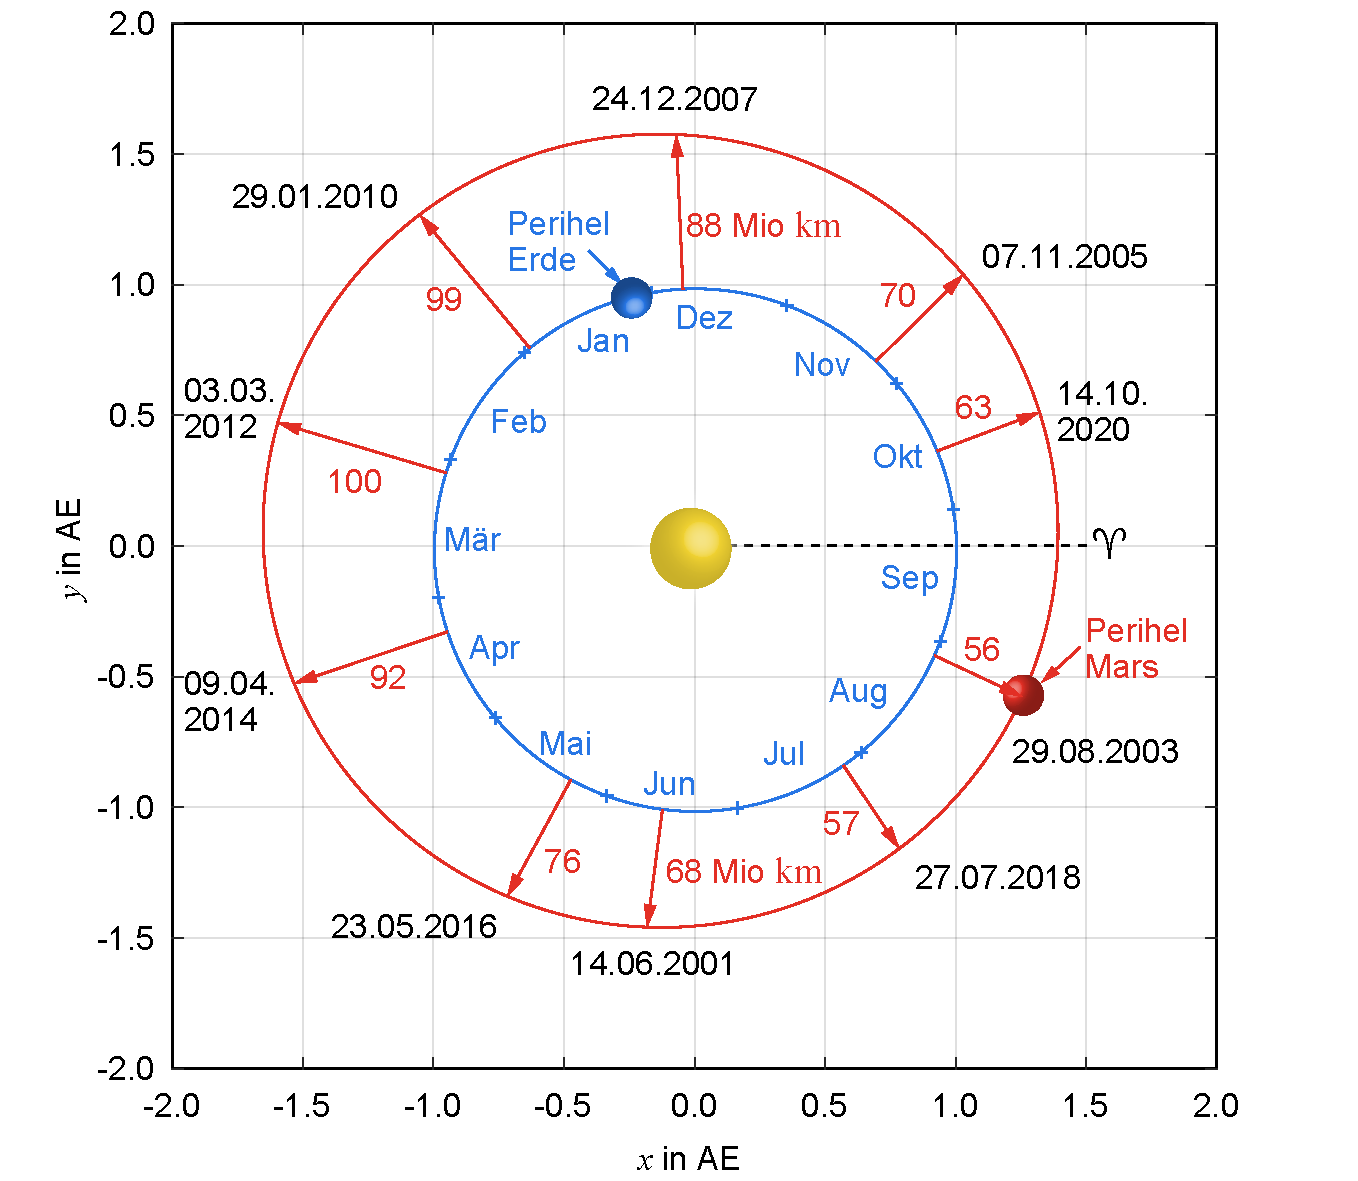
\includegraphics[width=\textwidth]{Mars_Opposition.pdf}%
\caption{Mars-Oppositionen im Zeitraum 2000 bis 2020}%
\label{abb:hm_mars_opposition_lsg}%
\end{figure}

\newpage
\begin{table}
\caption{Berechnung der Mars-Oppositionen von 2001 bis 2040}
\begin{tabular}{lR{1cm}R{1cm}R{1.5cm}R{1.5cm}R{1cm}R{1cm}R{1cm}R{1cm}}
\hline\noalign{\smallskip}
Datum	& $l\,[\degree]$ & $b\,[\degree]$ & $\Delta r\,[10^6\,\text{km}]$ & $R_\text{\mars}\,[10^6\,\text{km}]$ & $\beta\,[\degree]$ & $\delta\,[\degree]$ & $h\,[\degree]$ & $\text{Bw}\,['']$  \\
\noalign{\smallskip}\svhline\noalign{\smallskip}
14.06.2001 & 262.98 &	-1.02 &	67.80 &	219.10 &	-3.29 &	-26.54 &	14.66 &	20.60 \\
28.08.2003 & 335.09 &	-1.78 &	55.60	& 205.80 &	-6.62	& -15.79 &	25.41 &	25.13 \\
08.11.2005 & 45.70	& -0.13	& 70.40	& 218.00 &	-0.39	& 16.17	 &  57.37	& 19.85 \\
25.12.2007 & 93.05  &	1.27  & 88.60	& 235.00 &	3.38 &	26.78	 &  67.98	& 15.77 \\
30.01.2010 & 130.05	& 1.83	& 99.10	& 245.70 &  4.53	& 22.08	 &  63.28	& 14.10 \\
04.03.2012 & 163.78	& 1.69	& 100.40 & 248.00	& 4.17 &	10.23	 & 51.43	& 13.91 \\
10.04.2014 & 199.42 &	0.93	& 92.30	& 241.40	& 2.43	& -5.34	& 35.86	& 15.14 \\
23.05.2016 & 242.17	& -0.40	& 75.60	& 226.50	& -1.21	& -21.78 & 19.42 & 18.47 \\
27.07.2018 &	304.32 &	-1.79 &	57.40	& 208.50 & -6.49 & -25.48	& 15.72	& 24.32 \\
15.10.2020 &	21.49	& -0.87 &	62.70	& 211.20 & -2.94 &	5.65	& 46.85 & 22.28 \\
08.12.2022 &	76.10	& 0.83 &	82.10	& 228.80 &	2.31 &	25.01	& 66.21 &	17.02 \\
16.01.2025 &	116.10 &	1.70 &	96.00 &	242.40 &	4.29 &	25.14 &	66.34 &	14.55 \\
20.02.2027 &	150.93 &	1.81 &	101.00 & 248.10 &	4.46 &	15.31 &	56.51 &	13.83\\
25.03.2029 &	184.71 &	1.31 &	96.60	& 245.10 &	3.31 &	1.17 & 42.37 & 14.46 \\
04.05.2031 &	223.42 &	0.20 &	83.20	& 233.40 &	0.56 &	-15.33 & 25.87 &	16.79 \\
28.06.2033 &	276.69 &	-1.36 &	63.50	& 214.80 &	-4.59 &	-27.86 & 13.34 & 22.00 \\
17.09.2035 &	353.13 &	-1.54 &	57.00	& 206.60 &	-5.60	& -7.87 &	33.33	& 24.50 \\
20.11.2037 &	57.36  &	0.25 &	74.70	& 221.90 &	0.74 & 20.29 &	61.49	& 18.70 \\
03.01.2040 &	101.70 &	1.46 &	91.60	& 238.00 &	3.80 &	26.71 &	67.91 & 15.24 \\
\noalign{\smallskip}\hline\noalign{\smallskip}
\end{tabular}
\label{tab:hm_Mond-Mars-Abstand}
\end{table} 

In \figref{hm_mars_opposition_lsg} sind die Mars-Oppositionen f�r den Zeitraum 2000--2020 jeweils mit Datum und Abstand angegeben.
Man erkennt, dass bei Oppositionen in Periheln�he (z.\,B. am 29.08.2003) der Mars nahezu doppelt so gro� am Himmel erscheint\footnote{Tats�chlich konnte einer der Autoren (MK) am 29.08.2003 die Polkappen des Mars mit einem ZEISS APQ 135 ($5''$ Durchmesser und $2\:$m Brennweite) problemlos beobachten.
Gleich gute Chancen wird man in Europa erst wieder im Jahr 2035 haben.} wie bei Oppositionen in Apheln�he (z.\,B. am 03.03.2012).
Die Mars-Oppositionen f�r den Zeitraum 2001--2040 inklusive der f�r die Berechnung n�tigen Parameter sind in Tabelle \ref{tab:hm_Mond-Mars-Abstand} angegeben.\\

\medskip \end{sol}
\textcolor{blue} {$\rightarrow$ zur} \probref{hm_opposition_mars}.\\
\noindent\rule[1ex]{\textwidth}{0.5pt} \newpage


%-----------------------------------------------------------------------------------------------------------

\begin{sol}{prob:hm_venus_2004_2012}\label{lsg:hm_venus_2004_2012} %�bung18
\textbf{Venustransit-Beobachtungen 2004 und 2012} 

Vorbemerkung:\\
Beide Transits waren eine Jahrhundertereignis. Der n�chste Venustransit wird erst wieder 2117 zu beobachten sein. Wir bereiten mit dieser �bung aber schon mal die Berechnung vor. Ob man allerdings in 2117 noch eine \matlab{} Lizenz erwerben kann, ist nicht mit Sicherheit zu beantworten.

\begin{enumerate}[(a)] 
	\item Wir gehen von \figref{hm_VenusParallax} aus und betrachten den Fall, dass die Venus-Projektionen auf der Sonnenscheibe von den beiden Orten auf der Erde nicht symmetrisch zum Sonnenzentrum liegen.
          �ber die Geometrie der Winkel kann man zeigen, dass folgende Beziehungen gelten:
\begin{align*}
\nu_\text{\astrosun}+\nu_1 &= \nu_\text{\venus} + \nu_2 \\
\Rightarrow \Delta\nu &= \nu_1-\nu_2 ~~,
\end{align*}
woraus mit
\begin{align*}
\frac{\nu_\text{\venus}}{\nu_\text{\astrosun}} &= \frac{a_\text{\earth}}{a_\text{\venus}} \nonumber\\
\end{align*}
die Beziehung f�r die Astronomische Einheit 
\begin{equation}
a_\text{\earth} = \lk\frac{1}{\Delta\nu}\rk \lk\frac{d_\text{eff}}{\frac{a_\text{\earth}}{a_\text{\venus}} - 1}\rk = \frac{1}{\Delta\nu} \frac{d_\text{eff}}{\gamma - 1} \label{lsg:hm_venus_2004_2}
	\end{equation}
folgt.
\smallskip
Wir berechnen den effektiven Abstand $d_\text{eff}$ zwischen Troms� (N) und Canberra (AUS), in dem wir f�r die geographischen Koordinaten der Beobachtungsorte deren geozentrische Koordinaten verwenden.
Die Deklination f�r den Beobachtungsort entspricht dann der geographischen Breite (Abplattung der Erde vernachl�ssigt) und die Rektaszension ist einfach die Sternzeit berechnet nach \eqref{eq:hm_UT_3} zur Beobachtungszeit in UT.
Wir erhalten zu den Beobachtungsorten zwei Positions-Vektoren $\vec{r}_\text{T}$ und $\vec{r}_\text{C}$, deren Differenzvektor $\vec{r}_\text{d} = \vec{r}_\text{T}- \vec{r}_\text{C}$ unter einem Winkel $w$ zum Richtungsvektor Erdmittelpunkt -- Sonne ($\cos\delta\cos\alpha$, $\cos\delta\sin\alpha$, $\sin\delta$) steht.
Wir berechnen den Kosinus dieses Winkel $w$ aus dem Skalarprodukt.
Die effektive L�nge ist dann gegeben durch 
\begin{equation*}
d_\text{eff}=\left| \vec{r}_\text{d} \right|\sin w ~~.
\end{equation*}
F�r die Werte am 06.\,06.\,2012 sind die einzelnen Berechnungen in \mlhmref{VenusMerkurTransit.m} ausgef�hrt und numerisch ergibt sich $d_\text{eff}\!=\!11415 \:\text{km}$. \\
Ein sehr sch�ne Auswertung f�r die Berechnung der AE bei Beobachtung der Transitdauer an zwei Standorten findet sich in \cite{Messmer2004}. \\
\smallskip

	\item Wir gehen nun �ber zu der Auswertung der Transitdaten von nur einem Standort.
          Dazu muss man wie im  Beispiel \ref{bsp:venustransit} ausgef�hrt auf die t�gliche Parallaxe zur�ck greifen.
          Aus der Abbildung des Beispiels \ref{bsp:venustransit} k�nnen wir die folgende Beziehung ableiten:
	\begin{align}
	\frac{\D s_\text{\venus}-\D s_\text{\earth}}{a_\text{\earth}-a_\text{\venus}}&=\frac{\D P_\text{B} - \D s_\text{\earth}}{a_\text{\earth}}~,\nonumber\\
	\Rightarrow \frac{a_\text{\venus}}{a_\text{\earth}-a_\text{\venus}} \lk \frac{\D s_\text{\venus}}{a_\text{\venus}} - \frac{\D s_\text{\earth}}{a_\text{\earth}} \rk &= \frac{\D P_\text{B}}{a_\text{\earth}} ~,\nonumber \\
	\stackrel{\, 1/\D t}{\Rightarrow} \lk\frac{1}{\gamma -1}\rk \lk  \omega_\text{\venus} - \omega_\text{\earth} \rk &= \Omega_\text{B} ~~. \label{lsg:hm_venus_2004_3}
	\end{align}
Dabei haben wir $\gamma\!=\!a_\text{\earth} / a_\text{\venus}$, $\D s_i\!=\!\omega_i a_i \D t$ und $\D P_\text{B}\!=\!\Omega_\text{B} a_\text{\earth} \D t$ benutzt.
\smallskip
Wir berechnen den effektiven Abstand $d_\text{eff}$ f�r die Beobachtungen am 08.06.2004 in Oberkochen ($\phi\!=\!48.8\degree$ N, $\lambda\!=\!10.1\degree$ O) wieder wie oben, indem wir f�r die geographischen Koordinaten der Beobachtungszeitpunkte die geozentrische Koordinaten verwenden.
Die Deklination entspricht dann der geographischen Breite und die Rektaszensionen der Sternzeiten berechnet nach \eqref{eq:hm_UT_3} zum Anfangs- und Endzeitpunkt des Transits.
F�r gemessene Zeiten f�r Transitbeginn 07:16 MESZ $\pm 1$ min und Transitende 13:18 MESZ $\pm 1$ min ergibt sich eine effektive Entfernung von $d_\text{eff}\!=\!4444\:\text{km}$.
Die relative Sehnenl�nge konnte dabei zu 0.775 bestimmt werden (Messdaten MK).
Mit der Berechnungsformel aus dem Beispiel
\begin{equation}
a_\text{\earth}=\lk\frac{d_\text{eff}}{\gamma-1}\rk \lk\frac{1}{{l_\text{S\astrosun}}{b_\text{w\astrosun}}-\Omega_\text{B} T_\text{TR,B }}\rk \label{lsg:hm_venus_2004_4}
\end{equation}
erhalten wir daraus als Mittelwert f�r $\text{AE}\!=\!115\cdot 10^6\:$km.
Tr�gt man den relativen Fehler als Funktion der gemessenen Transitzeit auf, so sieht man, dass schon bei Unsicherheiten in der gemessenen Transitzeit von $60\:\text{s}$ ein Fehler von $20\%$ in der Bestimmung der astronomischen Einheit resultiert (\figref{hm_Kontaktzeit_lsg}a.
Das liegt daran, dass die Abh�ngigkeit von der gemessenen Transitzeit, bei dem gegen Null gehenden Nenner in \eqref{lsg:hm_venus_2004_3} sehr gro� ist (\figref{hm_Kontaktzeit_lsg}b.
Genau so kritisch ist die Messung der Sehnenl�nge $l_\text {S}$ des Transits.
Im Rahmen der Messgenauigkeit ergab sich ein Mittelwert von $115\cdot 10^6\:\text{km} $.\footnote{Der Mittelwert ist tendenziell ein eher zu kleiner Wert, was vermuten l�sst, dass die Messzeit als zu kurz eingesch�tzt wurde.
Es ist au�erordentlich schwierig, am Rand der Sonne genau Beginn und Ende des Transits festzustellen.}
\begin{figure}[H]
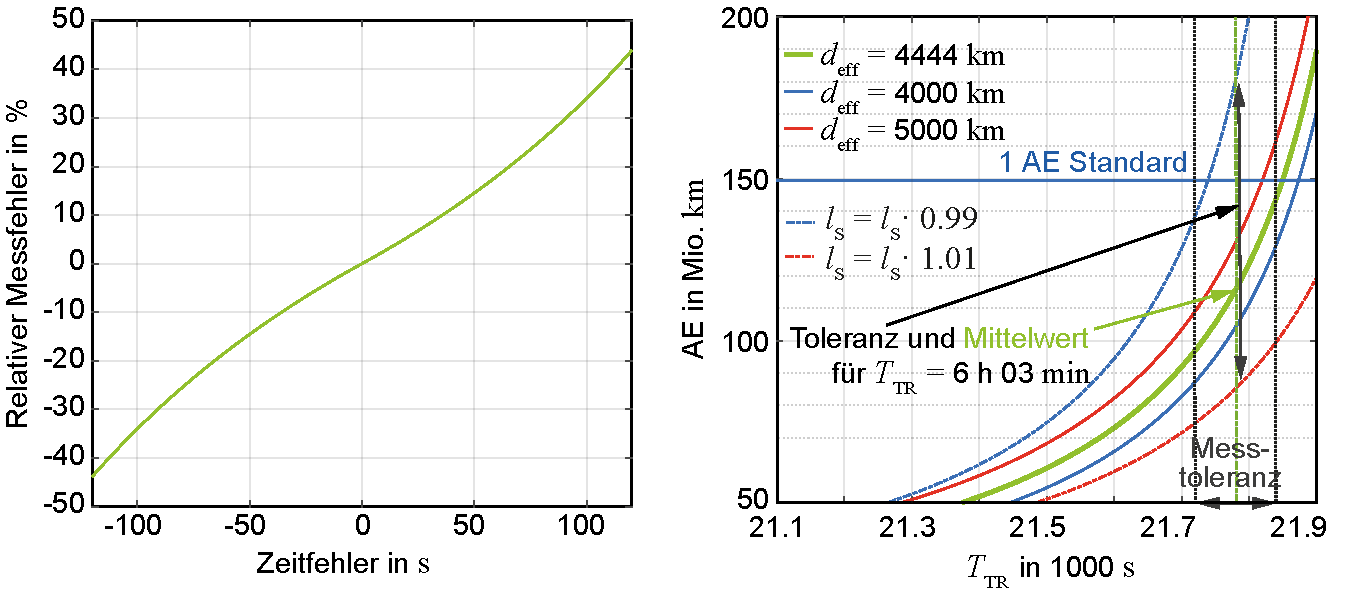
\includegraphics[width=\columnwidth]{KontaktzeitmethodeAE.pdf}%
\caption{Fehler in der Bestimmung der AE bei der Kontaktzeitmethode}%
\label{abb:hm_Kontaktzeit_lsg}%
\end{figure}
Ein verbesserte Auswertung f�r die Berechnung der AE bei Beobachtung der Transitdauer an nur einem Standorten findet sich \cite{Brodbeck2004}. \\

	\item Wir ber�cksichtigen jetzt f�r den Fall, dass die Beobachtung nur an einem Ort der Erde stattfinden kann.
          sowohl die Elliptizit�t der Bahnen, als auch die Neigung der Venusbahn gegen die Ekliptik und die topozentrischen Koordinaten des Beobachters.
          Diese Berechnung geht auf den Astronomen James Short\footnote{James Short (1710--1768) war ein britischer Mathematiker, Optiker und begnadeter Teleskopbauer.
          Wir empfehlen dazu auch den lesenswerten Artikel \cite{Teets2003}, auf dessen Basis die L�sung der �bung strukturiert wurde.} zur�ck, der viele der Messungen von 1761 systematisch auswertete und dessen ermittelte Sonnenparallaxe von $8.65''$ �quivalent zu $a_\text{\earth}\!=\!154.4\cdot 10^6 \:\text{km}$ lange als Referenz f�r die AE galt.
          Die Rechnungen sind im Detail in \mlhmref{VenusMerkurTransit.m} ausgef�hrt.
          Eine Betrachtung f�r n�herungsweise konzentrisch und koplanar angenommene Planetenbahnen kann man in \cite{Messmer2004} bzw. \cite{Brodbeck2004} finden. \\
Um den Transit in seiner allgemeinen Form zu berechnen, m�ssen wir zwei KOS zueinander in Beziehung setzen:
\begin{enumerate}[A.]
	\item Das GA(sf) KOS (\figref{hm_venustransit_lsg_2a}), was f�r den Beobachter des Transits das ausgezeichnete KOS ist und folgenderma�en definiert ist:
	Die $x'$-Achse zeigt zum Fr�hlingspunkt und beh�lt ihre Richtung im Raum bei, die $z'$-Achse ist die Rotationsachse der Erde.
	\begin{enumerate}[1.]
	\item Die t�gliche Rotation der Erde beschreiben wir mit 
\begin{equation}
\theta = \theta_0 + \frac{15\degree}{\text{h}}\, (t-t_0)~~,
\label{eq:hm_venustr_d_3}
\end{equation}
worin $\theta_0\!=\!\GMST$ und die Zeiten $t$, $t_0$ in UT angegeben werden.
$t_0$ soll dabei die Zeit der Transitmitte sein.
\begin{figure}[H]
	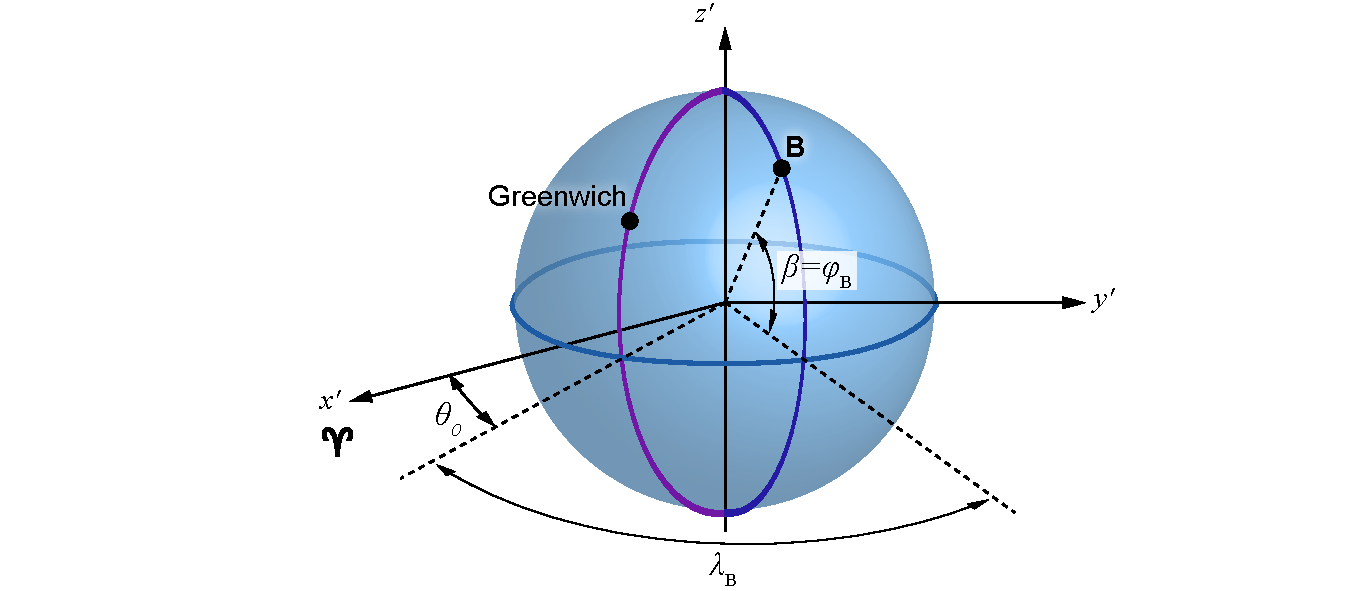
\includegraphics[width=\textwidth]{VenustransitKS.pdf}%
	\caption[Koordinatensystem des Beobachters beim Venustransit.]{Koordinatensystem ($x'$-$y'$-$z'$) des Beobachters beim Venustransit}%  
	\label{abb:hm_venustransit_lsg_2a}%
\end{figure}
	\item F�r die Koordinaten $\vec{r}'$ rechnen wir die geographischen Koordinaten $\varphi_\text{B}$, $\lambda_\text{B}$ eines Beobachters B in geozentrisch-�quatoriale Koordinaten um, wobei die Abplattung der Erde vernachl�ssigt wird und deshalb $\beta\!=\!\varphi_\text{B}$ ist.
          Damit gilt 
\begin{equation}
\vec{r}' = \lk\begin{matrix} x' \\ y' \\ z'\end{matrix}\rk = \mathbb{R}_\text{\earth}\,\lk\begin{matrix} \cos\beta\cos(\theta+\lambda_\text{B})\\ \cos\beta\sin(\theta + \lambda_\text{B})\\ \sin\beta \end{matrix}\rk ~~.
\label{eq:hm_venustr_d_2}
\end{equation}
\end{enumerate}	
	\begin{figure}[H]
	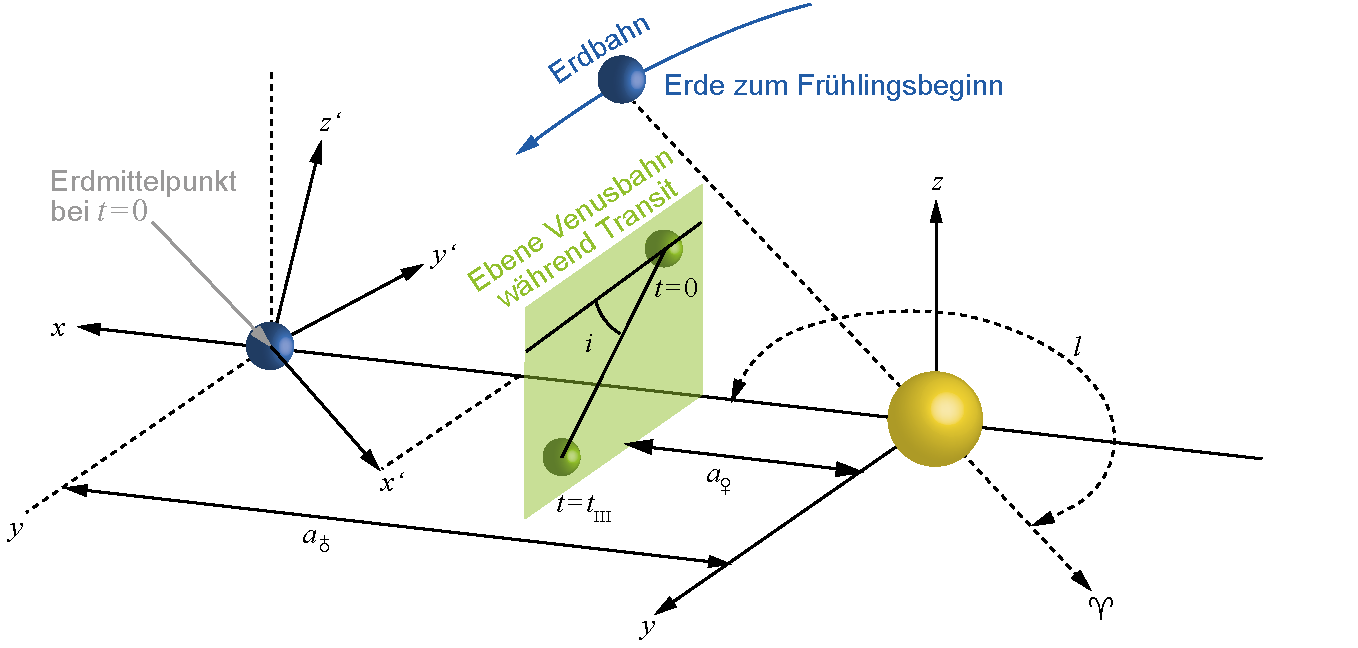
\includegraphics[width=\textwidth]{VenustransitHelioKS.pdf}%
	\caption[Beziehungen der Koordinatensysteme beim Venustransit.]{Beziehung des heliozentrischen Koordinatensystems ($x$, $y$, $z$) und des Koordinatensystems des Beobachters ($x'$, $y'$, $z'$) beim Venustransit}% 
	\label{abb:hm_venustransit_lsg_2b}%
	\end{figure}
	
	\item Das HE-KOS, welches f�r die Beschreibung der Planetenbewegung das geeignete ist.
          Bei diesem zeige die $x$-Achse nicht zum Fr�hlingspunkt, sondern zum Mittentransitzeitpunkt genau zum Erdmittelpunkt.
	\item Die Beziehung zwischen den kartesischen Koordinaten beider KOS ergibt sich nach \figref{hm_venustransit_lsg_2b} gem��:
	\begin{enumerate}[1.] 
	\item Translation
\begin{align}
	\vec{r} &= \mathbb{R}_z(-l)\,\mathbb{R}_y(-\epsilon)\,\vec{r}' + \vec{r}_\text{\earth\astrosun} \nonumber\\
	\smallskip
	\lk\begin{matrix} x \\ y \\ z \end{matrix}\rk &= \lk\begin{matrix} \cos l & \sin l & 0 \\ -\sin l & \cos l & 0 \\ 0 & 0 & 1\end{matrix}\rk \lk\begin{matrix} 1 & 0 & 0 \\ 0 & \cos\epsilon & \sin\epsilon \\ 0 & -\sin\epsilon & \cos\epsilon \end{matrix}\rk \lk\begin{matrix} x' \\ y' \\ z' \end{matrix}\rk + \lk\begin{matrix} a_\text{\earth} \\ 0 \\ 0 \end{matrix}\rk ~~. \label{eq:hm_venustr_d_1}
\end{align}
\item W�hrend der halben Dauer des Transits bewegt sich die Erde mit ihrer Winkelgeschwindigkeit $\omega_\text{\earth}$ weiter um die Sonne.
  Wir nehmend etwas vereinfachend an, dass diese Bewegung in der betrachtet kurzen Zeitspanne nur entlang der $y$-Achse erfolgt.
  D.\,h. wir haben 
\begin{equation}
\Delta \vec{r} = \lk\begin{matrix} 0 \\ \omega_\text{\earth}t \\ 0 \end{matrix}\rk ~~.
\label{eq:hm_venustr_d_4}
\end{equation}
Addiert man \eqref{eq:hm_venustr_d_4} und \eqref{eq:hm_venustr_d_1}, erh�lt man mit \eqref{eq:hm_venustr_d_2} und \eqref{eq:hm_venustr_d_3} f�r $\vec{r}'$ die Koordinaten des Beobachters zu einem beliebigen Zeitpunkt $t$ w�hrend des Transits.
\end{enumerate}
\end{enumerate}
\begin{figure}[H]
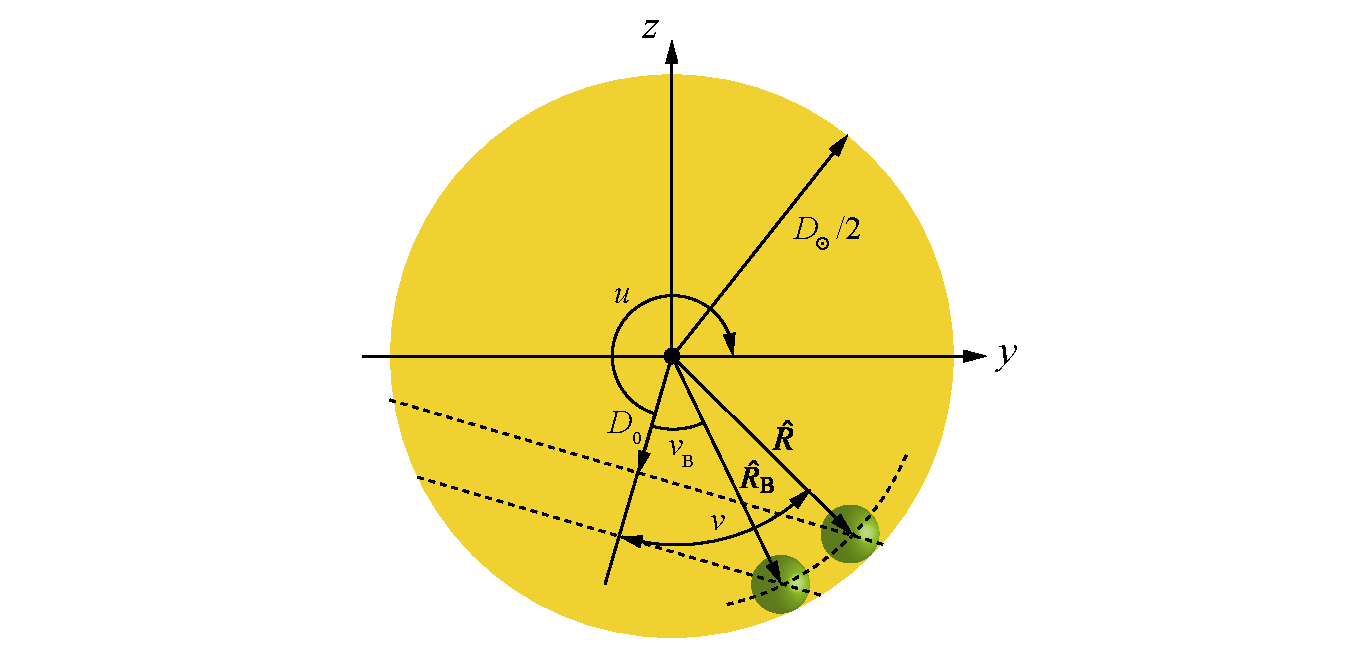
\includegraphics[width=\textwidth]{VenustransitGeometrie.pdf}%
\caption{Geometrie des Venustransits}%
\label{abb:hm_venustransit_lsg_3}%
\end{figure}

Wir betrachten nun als angenommener Beobachter im Erdmittelpunkt die Position der Venusprojektion vor der \anf{Sonnenscheibe} in \figref{hm_venustransit_lsg_3}.
Dabei m�ssen wir uns noch einmal klarmachen, dass zu jedem Zeitpunkt des Transits Erdmittelpunkt, Venusmittelpunkt und der Mittelpunkt des Venus-Projektionsscheibchens auf der Sonne auf einer Linie liegen.
F�r die Projektionsposition $\vec{r}_\text{P,0}$ (Mitte des Transits $t\!=\!0$) ergibt sich dann f�r die Position der Venus im $x,y,z$-KOS:
\begin{equation}
\gamma \lk \vec{r}_\text{\venus,0} - \vec{r}_\text{P,0} \rk =  \lk \vec{r}_\text{\earth,0} - \vec{r}_\text{P,0}\rk ~,
\label{eq:hm_venustr_d_5}
\end{equation}
worin $\gamma = a_\text{\earth}/a_\text{\venus}$ ist und 
\begin{equation*}
\vec{r}_\text{\earth,0} = \lk\begin{matrix} a_\text{\earth} \\ 0 \\ 0\end{matrix}\rk ~~\text{und}~~ \vec{r}_\text{P,0} = \lk\begin{matrix} 0 \\ D_0\cos u \\ D_0\sin u\end{matrix}\rk
\end{equation*}
jeweils die Positionen des Erdmittelpunktes und die Mitte des Projektionsscheibchens zum Transitmittenzeitpunkt sind.
F�r einen sp�teren Zeitpunkt $t$, z.\,B. dem Zeitpunkt des sogenannten 3. Kontakts $t_\text{III}$ gilt analog
\begin{equation}
\gamma \lk \vec{r}_\text{\venus,III} - \vec{r}_\text{P,III} \rk = \lk \vec{r}_\text{\earth,III} - \vec{r}_\text{P,III} \rk ~,
\label{eq:hm_venustr_d_6}
\end{equation}	
worin
\begin{equation*}
\vec{r}_\text{P,III} = \lk\begin{matrix} 0 \\ \hat{R}\cos(u+v) \\ \hat{R}\sin(u+v)\end{matrix}\rk ~~\text{mit}~~ \hat{R} = \frac{D_\text{\astrosun}}{2} - R_\text{P} ~~.
\end{equation*}	
Hierin ist $R_\text{P}$ der Radius des Projektionsscheibchens auf der Sonne und $D_\text{\astrosun}$ der Durchmesser der Sonne, jeweils in Winkelma�en angegeben.
F�r die Koordinaten $\vec{r}_\text{\venus,III}$ und $\vec{r}_\text{\earth,III}$ m�ssen wir die planetare Bewegung ber�cksichtigen (\figref{hm_venustransit_lsg_2b}), so dass dann folgt:
\begin{align}
	\vec{r}_\text{\earth,III} &= \lk\begin{matrix} a_\text{\earth} \\ \omega_\text{\earth} t_\text{III} \\ 0\end{matrix}\rk ~~, \nonumber\\
	\vec{r}_\text{\venus,III} &= \vec{r}_\text{\venus,0} + a_\text{\venus} \omega_\text{\venus} t_\text{III}\,\lk\begin{matrix} 0 \\ \cos i \\ -\sin i\end{matrix}\rk ~~. \label{eq:hm_venustr_d_7}
\end{align}	
Darin haben wir die Bewegung der Erde entlang der Richtung der $y$-Achse und die der Venus in der $y,z$-Ebene angenommen.
Die Bahnneigung der Venus gegen�ber der Ekliptik ist damit ber�cksichtigt, $\vec{r}_\text{\venus,0}$ ist durch \ref{eq:hm_venustr_d_5} gegeben.
Mit \eqref{eq:hm_venustr_d_5} bis \eqref{eq:hm_venustr_d_7} haben wir den Transit nun vollst�ndig f�r einen \anf{hypothetischen} Beobachter im Erdmittelpunkt beschrieben.
Wir wollen jetzt die Transitzeit bzw. die Zeit des 3. Kontakts bestimmen.
Wir erhalten aus der $y$-Komponente der Gleichung \eqref{eq:hm_venustr_d_6}
\begin{equation}
\sin u = \frac{a_\text{\venus} (\omega_\text{\earth} - \omega_\text{\venus}\cos i) }{(a_\text{\earth} - a_\text{\venus})\,\sqrt{\hat{R}^2 - D_0^2}}\,t_\text{III}
\label{eq:hm_venustr_d_8}
\end{equation}
und analog f�r die $z$-Komponente
\begin{equation}
\cos u = \frac{a_\text{\venus} \omega_{\venus} \sin i}{(a_\text{\earth} - a_\text{\venus})\,\sqrt{\hat{R}^2 - D_0^2}}\,t_\text{III} ~~.
\label{eq:hm_venustr_d_9}
\end{equation}	
Wegen $\cos^2 u + \sin^2 u\!=\! 1$ folgt aus \eqref{eq:hm_venustr_d_8} und \eqref{eq:hm_venustr_d_9}
\begin{equation*}
t_\text{III} = \lk \frac{a_\text{\earth}}{a_\text{\venus}} - 1 \rk\,\sqrt{\frac{\hat{R}^2 - D_0^2}{\omega_\text{\venus}^2 + \omega_\text{\earth}^2 - 2\omega_\text{\venus} \omega_\text{\earth} \cos i}} ~~.
\end{equation*}	
Man erkennt, dass f�r die im Beispiel \ref{bsp:venustransit} gemachte N�herung der koplanaren Bahnen sich tats�chlich die gesamte Transitzeit n�herungsweise zu	
\begin{equation*}
T_\text{TR} = 2t_\text{III} \approx (\gamma -1)\,\lk\frac{l_\text{s}}{\omega_\text{\venus} - \omega_\text{\earth}}\rk
\end{equation*}
ergibt.
Jetzt gehen wir vom Erdmittelpunkt zu einem Beobachter auf der Erdoberfl�che bei $(\varphi_\text{B},\lambda_\text{B})$ �ber.
Wir wissen aus der Geometrie, dass dessen beobachtete Zeit des 3. Kontakts $t_\text{III}^\text{(B)}\!\neq\! t_\text{III}$ ist.
Ebenso hat f�r ihn das Bild der Venus auf der Sonne bei $t\!=\!t_\text{III}^\text{(B)}$ andere Koordinaten als f�r den gedachten Beobachter im Erdmittelpunkt.
\begin{equation}
\vec{r}_\text{P,III}^\text{(B)} = \lk\begin{matrix} 0 \\ y_\text{P} \\ z_\text{P}\end{matrix}\rk ~~\text{mit}~~ \hat{R}_\text{B} = \hat{R} = \sqrt{y_\text{P}^2 + z_\text{P}^2} ~~.
 \label{eq:hm_venustr_d_10}
\end{equation}
Die Position des Beobachters auf der Erdoberfl�che zum Zeitpunkt $t\!=\!t_\text{III}^\text{(B)}$ ist demnach durch
\begin{equation}
\vec{r}_\text{\earth,III}^\text{(B)} = \lk \begin{matrix} x^\text{(B)} \\ y^\text{(B)} \\ z^\text{(B)} \end{matrix} \rk + \lk \begin{matrix} 0 \\ \omega_\text{\earth}t_\text{III}^\text{(B)} \\ 0 \end{matrix}\rk ~~.
\label{eq:hm_venustr_d_11}
\end{equation}
gegeben.
Die Position der Venus zu diesem Zeitpunkt ergibt sich aus \eqref{eq:hm_venustr_d_7} zu
\begin{equation}
\gamma \lk \vec{r}_\text{\venus,III}^\text{(B)} - \vec{r}_\text{\venus,0}^\text{(B)} \rk = \omega_\text{\venus} t_\text{III}^\text{(B)}\,\lk\begin{matrix} 0 \\ \cos i \\ -\sin i \end{matrix}\rk ~~.
\label{eq:hm_venustr_d_12}
\end{equation}
Der Vektor $\vec{r}_\text{\venus,III}^\text{(B)} - \vec{r}_\text{P,III}^\text{(B)}$ muss wiederum ein konstantes Vielfaches $k$ des Vektors $\vec{r}_\text{\earth,III}^\text{(B)} - \vec{r}_\text{P,III}^\text{(B)}$ sein, wie man sich leicht geometrisch klarmachen kann.
Wir erhalten aus der $x$-Komponente $k\!=\!a_\text{\venus}/x^\text{(B)}$, worin $x^\text{(B)}$ die Koordinate der Beobachterposition im kartesischen $x,y,z$ KOS zur Zeit $t_\text{III}^\text{(B)}$ ist.
Damit f�gen wir eine messbare L�ngendimension in das Gleichungssystem ein.
Analog erh�lt man f�r die $y$- und $z$-Komponenten von \eqref{eq:hm_venustr_d_10}
\begin{align*}
	y_\text{P} &= M + Nt_\text{III}^\text{(B)}~~,\\
	z_\text{P} &= P + Qt_\text{III}^\text{(B)}
\end{align*}
mit
\begin{align}
	M &= \frac{(\gamma-1)x^\text{(B)}\,D_0\cos u - y^\text{(B)}}{x^\text{(B)}/a_\text{\venus} - 1} ~~, \label{eq:hm_venustr_d_13} \\
	N &= \frac{x^\text{(B)}\omega_\text{\venus} \,\cos i - \omega_\text{\earth}}{x^\text{(B)}/a_\text{\venus} - 1} ~~, \nonumber\\
	P &=  \frac{(\gamma-1)x^\text{(B)}\,D_0\sin u - z^\text{(B)}}{x^\text{(B)}/a_\text{\venus} - 1} ~~, \nonumber \\
	Q &= \frac{x^\text{(B)} \omega_\text{\venus}\,\sin i}{x^\text{(B)}/a_\text{\venus} - 1} ~~. \nonumber
\end{align}
Wegen $y_\text{P}^2 + z_\text{P}^2\!=\!\hat{R}^2$ folgen schlie�lich die Relationen
\begin{align}
	\hat{R}^2 &= \lk M + Nt_\text{III}^\text{(B)}\rk^2 + \lk P - Qt_\text{III}^\text{(B)}\rk^2 ~~, \label{eq:hm_venustr_d_14} \\
	R^2 &= M^2 + 2NMt_\text{III} + N^2 t_\text{III}^2 + P^2 - 2PQt_\text{III} + Q t_\text{III}^2  ~~,\nonumber \\
	0 &= t_\text{III}^2 \lk N^2 + Q^2 \rk^2 + 2t_\text{III} (MN - PQ) + M^2 + P^2 - \hat{R}^2  ~~,\nonumber\\
	t_\text{III}^\text{(B)} &= -(MN - PQ) + \sqrt{(MN - PQ)^2 + \hat{R} - M^2 - P^2}  ~~.\nonumber
\end{align}
Damit hat man f�r einen Beobachter auf der geographischen Position $\varphi_\text{B},\lambda_\text{B}$ die Zeitdifferenz $t_\text{III}^\text{(B)} - t_\text{III}$ bei der Beobachtung des 3. Kontakts gegen�ber einem hypothetischen Beobachter im Erdmittelpunkt erhalten.
Hat man zwei Beobachter an zwei Orten, so kann man den hypothetischen Beobachter im Erdmittelpunkt eliminieren und betrachtet nur die Messungen der beiden Beobachter auf der Erdoberfl�che.
In $M$, $N$, $P$ und $Q$ sind mit Ausnahme von $a_\text{\venus}$ alle anderen Gr��en bekannt, also $D_0$, $u$, $\hat{R}$, $\omega_\text{\venus}$, $\omega_\text{\earth}$, $\gamma$ und $i$.
Man kann daher �ber einen Fit an $t_\text{III}^\text{(B)}(a_\text{\venus})$ f�r die Zeitdifferenz zweier Beobachtungssituationen den Abstand der Venus bestimmen und �ber das 3. Keplergesetz die Astronomische Einheit berechnen.\\
Sehr instruktiv ist eine "`Vorw�rtsrechnung"', d.h. eine Berechnung der relativen geozentrisch-�quatorialen Koordinaten von Sonne und Venus oder der entsprechenden topographisch-horizontalen Koordinaten (Achtung: hier wirklich topographische Koordinaten verwenden !) mit den heute verf�gbaren Daten aus der St�rungsrechnung.
Siehe auch Zusatzaufgabe \ref{prob:hm_Zusatz_VenusTransit_Vorwaerts}.
Ergebnisse daraus sind im hier f�r den Venustransit von 2004 angegeben (\mscr~\mlhmref{VenusTransit01.m} und \mlhmref{VenusTransit02.m}:). \\
\vspace{0.5 cm}
\begin{tabular}{L{4cm}R{2cm}R{2cm}}
\hline\noalign{\smallskip}
Ort & $t_\text{III}^\text{(B)} - t_\text{III}$ (berechnet) & beobachtet \\
\noalign{\smallskip}\svhline\noalign{\smallskip}
Oberkochen & $-1\:\text{min}\,12\:\text{s}$ & $-1\:\text{min}\,11\:\text{s}$ \\
Troms� & $-1\:\text{min}\,12\:\text{s}$ & \\
Canberra   &  $6\:\text{min}\,12\:\text{s}$ & \\
\end{tabular} 
\vspace{1 cm}
\\
Bemerkungen:
\begin{itemize}
	\item Bemerkung 1\\
Will man die Methode f�r den Transit an nur einem Standort benutzen, so muss man \eqref{eq:hm_venustr_d_14} etwas modifizieren.
Es ist relativ einsichtig, dass die Koordinaten $x^\text{(B)}$, $y^\text{(B)}$ und $z^\text{(B)}$ von $M$, $N$, $P$ und $Q$ von $t_\text{III}^\text{(B)}$ abh�ngen und zu einer bestimmten Zeit berechnet werden m�ssen (\ldots Unterschied zwischen UT und ET beachten!).
Die Gleichungen \eqref{eq:hm_venustr_d_14} sind dann vom Typ
\begin{equation*}
t_\text{III}^\text{(B)} = f(t_\text{III}^\text{(B)},a_\text{\venus})~~,
\end{equation*}
die numerisch nach $a_\text{\venus}$ gel�st werden kann.\\
\item Bemerkung 2\\
Eine v�llig analoge und gleichzeitig sehr instruktive Betrachtung kann man anstellen, wenn man berechnet wie der Venusschatten die Erde trifft.
Diese Methode ist ausf�hrlich in \cite{Backhaus2012} mit Daten f�r den Venustransit von 2012 beschrieben.\\
\item Bemerkung 3\\
Mit zuk�nftigen Marsmissionen wird man nicht bis zum n�chsten Venustransit warten m�ssen, um wieder einen Planeten vor der Sonne vor�berziehen zu sehen.
Nat�rlich gelten alle bisher gemachten �berlegungen auch f�r einen Beobachter auf dem Mars.
Dieser kann dann nat�rlich auch beobachten, wie unsere Erde und ihr Mond vor der Sonne vor�berziehen.
Das letzte Ereignis dieser Art war am 11. Mai 1984 und das n�chste ist am 10.November 2084.
Wir sind aber nicht sicher, ob bereits jetzt Anmeldungen entgegen genommen werden.
Wir empfehlen das mit dem \mscr~\mlhmref{InnerePlaneten.m} \bzw \mlhmref{VenusTransit01.m} zu �berpr�fen.
F�r eine genauere Rechnung der Transitzeiten benutzen Sie die Koordinatenberechnungen nach der St�rungstheorie, d.h. die Funktionen \mlhmiref{SonneExakt.m} und \mlhmiref{MarsExakt.m}.
Siehe auch Zusatzaufgabe \ref{prob:hm_Zusatz_ErdeTransit_from_Mars}.\\
\end{itemize}
\end{enumerate}
\medskip \end{sol}
\textcolor{blue} {$\rightarrow$ zur} \probref{hm_venus_2004_2012}.\\
\noindent\rule[1ex]{\textwidth}{0.5pt} \newpage


%-----------------------------------------------------------------------------------------------------------

\begin{sol}{prob:hm_jupiterbedeckung_venus} \label{lsg:hm_jupiterbedeckung_venus} %�bung19
\textbf{Jupiterbedeckung durch die Venus am 22.11.2065} \\ \\
Die Rechnungen sind im Detail in \mlhmref{PlanetenbahnenKepler.m} ausgef�hrt. \\

\begin{figure}[H]
\begin{minipage}{\textwidth}
\leftfigure{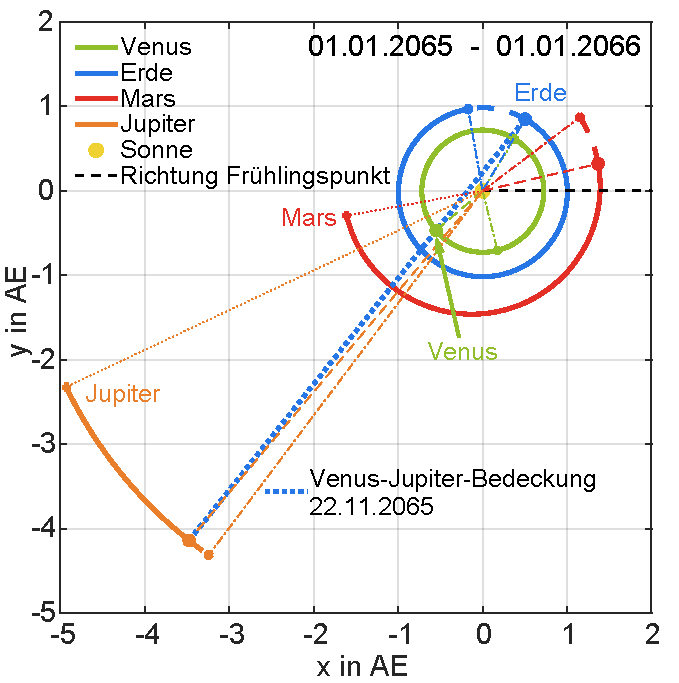
\includegraphics[width=0.5\textwidth]{JupiterBedeckung.pdf}}
\hspace{\fill}
\rightfigure{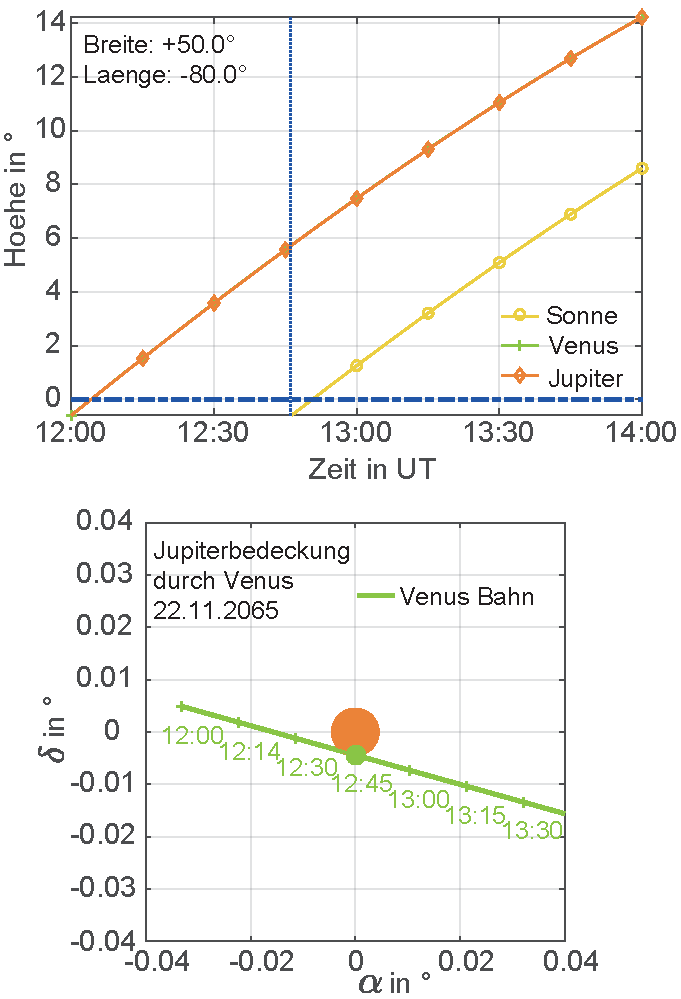
\includegraphics[width=0.5\textwidth]{JupiterVenus.pdf}}
\leftcaption{Konstellation der Planeten am 22.11.2065}\label{abb:hm_JupiterBedeckung_lsg}
\rightcaption{Jupiterbedeckung durch Venus am 22.11.2065}\label{abb:hm_JupiterVenus_lsg}
\end{minipage}
\end{figure}

Aufgrund der erforderlichen Pr�zision wurden die im \matlab{} Programm die hinterlegten Routinen \mlhmiref{VenusExakt.m} und \mlhmiref{JupiterExakt.m} f�r die Berechnung der Planetenpositionen benutzt.
Diese auf den Reihenentwicklungen der St�rungstheorie entwickelten Routinen wurden \cite{Montenbruck1999} entnommen und liefern Genauigkeiten von besser als 10 Bogensekunden �ber den Zeitraum von ca. 50 Jahren.\\
Leider ist die Bedeckung des Jupiters durch die Venus nicht ganz vollst�ndig und noch dazu sehr ung�nstig zu beobachten, da beide Planeten einen relativ geringen Winkelabstand zur Sonne haben.
Am ehesten hat man eine Chance in Nordamerika.

\medskip \end{sol}
\textcolor{blue} {$\rightarrow$ zur} \probref{hm_jupiterbedeckung_venus}.\\
\noindent\rule[1ex]{\textwidth}{0.5pt} \newpage


%%%-----------------------------------------------------------------------------------------------------------

\subsection{�bungen zu Himmelsbeobachtungen von anderen Planeten aus}

\medskip

%-----------------------------------------------------------------------------------------------------------

\begin{sol}{prob:hm_erdaufgang_von_mond} \label{lsg:hm_erdaufgang_von_mond} %�bung20
\textbf{Kann man einen Erdaufgang vom Mond aus sehen?} \\ \\
Als erste Reaktion w�rde man sagen, dass auf dem Mond keine Erdauf- bzw. unterg�nge beobachtet werden k�nnen, da ein Beoabachter auf der Mondvorderseite wegen der gebundenen Rotation (\vgl auch L�sung \ref{lsg:hm_erdrotation}) immer die Erde sieht, wenn auch in verschiedenen Beleuchtungsphasen, so wie wir den Mond sehen.
Diese Behauptung gilt aber nur f�r eine exakt kreisf�rmige Bahn.
Auf Grund der relativ starken Elliptizit�t der Mondbahn und der daraus folgenden unterschiedlichen Geschwindigkeiten, zeigt der Mond der Erde immer ein leicht anderes Antlitz.
Er \anf{sch�ttelt} sozusagen den Kopf (Wir hoffen, dass dies nicht als Missfallen gegen�ber den hier gemachten physikalischen Betrachtungen gedeutet werden muss.).
Dieser Effekt ist schon seit dem Mittelalter als \emph{Libration} bekannt.
Die Libration kann einfach abgesch�tzt werden, indem man das Erde-Mond-System als ZKP betrachtet und die maximale Differenz von wahrer und mittlerer Anomalie berechnet.\\
Mit den Werten f�r die Exzentrizit�t $e_\text{Mond}\!=\!0.0549$ ergibt sich mit den ersten Termen der Mittelpunktsgleichung \eqref{eq:hm_mpglg_nu-M}, wenn f�r die mittlere Anomalie $M_\text{Mond} (t)\!= \!134.96\degree + 13.06\degree \, t \; \text{in} [\degree/\text{d}$] der Wert $90\degree$ oder $270\degree$ eingesetzt wird (der Zeitpunkt $t$ spielt f�r uns jetzt keine Rolle):
\begin{equation*}
	\delta \,l_\text{lib} = C_\text{Mond,max} \approx \upsilon - M_\text{Mond,max} = 2e_\text{Mond} + \frac{5}{5}e_\text{Mond}^3\! + \ldots \approx 0.11 \approx 6.3\degree ~~.
\end{equation*}
Die tats�chliche Libration betr�gt etwa $7.9\degree$.
Der Unterschied von ca. $1.6\degree$ kommt durch den zus�tzlichen Einfluss der Sonne zustande.
Die Erde erscheint vom Mond betrachtet unter einem Winkel 
\begin{equation*}
	2\alpha = \arctan \lk\frac{R_{\earth}}{a_{{\earth}\text{Mond}}} \rk \approx 1.9\degree ~~, 
\end{equation*}
was deutlich kleiner ist als $\delta l_\text{lib}$.
Man kann also vom Mond aus den Erdaufgang sehen, vorausgesetzt man befindet sich in den \anf{Randbereichen} des Mondes (bei selenographische L�ngen um $90\degree$) oder in einem Raumschiff (\probref{hm_erdaufgang_von_apollo}).
Der Landeplatz von Apollo 11 war allerdings bei bei einer selenographischen Position von $0\degree$N und $23.5\degree$W (also nahe des Mond�quators), so dass Armstrong\indexp{Armstrong, Neil Alden} und Aldrin\indexp{Aldrin, Buzz} diese Beobachtung nicht verg�nnt war.
Abgesehen davon, waren sie nicht lang genug auf dem Mond, denn die Periode der Libration ist in etwa so lang wie der anomalistische Monat von ca. $27.5$ Tagen.
Man kommt also in den entsprechenden Bereichen nur einen Tag im Monat in den Genuss des Erdaufgangs.\\
\medskip \end{sol}
\textcolor{blue} {$\rightarrow$ zur} \probref{hm_erdaufgang_von_mond}.\\
\noindent\rule[1ex]{\textwidth}{0.5pt} \newpage

%-----------------------------------------------------------------------------------------------------------

\begin{sol}{prob:hm_erdaufgang_von_apollo}\label{lsg:hm_erdaufgang_von_apollo} %�bung21
\textbf{Earth Rise von Apollo 8} \\ \\
Wie man aus \figref{hm_EarthRise_calc} sieht, m�sste man das von Apollo 8 aufgenommene Bild eigentlich um $90\degree$ gegen den Uhrzeigersinn drehen, die Sonne kam von links.
Wenn man noch wei�, dass Apollo 8 zu dieser Zeit auf einer elliptischen Bahn war, deren Pericynthion (mondnaher Punkt) bei $\SI{112}{\kilo\metre}$ und deren Apocynthium (mondferner Punkt) bei $\SI{312}{\kilo\metre}$  lagen, sowie die Umlaufbahn um zwei Grad gegen den Mond�quator geneigt war, kann man auch relativ genau die Position des Raumschiffs berechnen (Zusatzaufgabe).  F�r Interessanten haben wir im \mscr{} \mlhmref{Apollo8LunarOrbit.m} die Bahn und den Zeitpunkt des Earth Rise Fotos mit den Daten des jPL berechnet und dargestellt.

\medskip \end{sol}

\begin{figure}[H]
\begin{minipage}{\textwidth}
\leftfigure{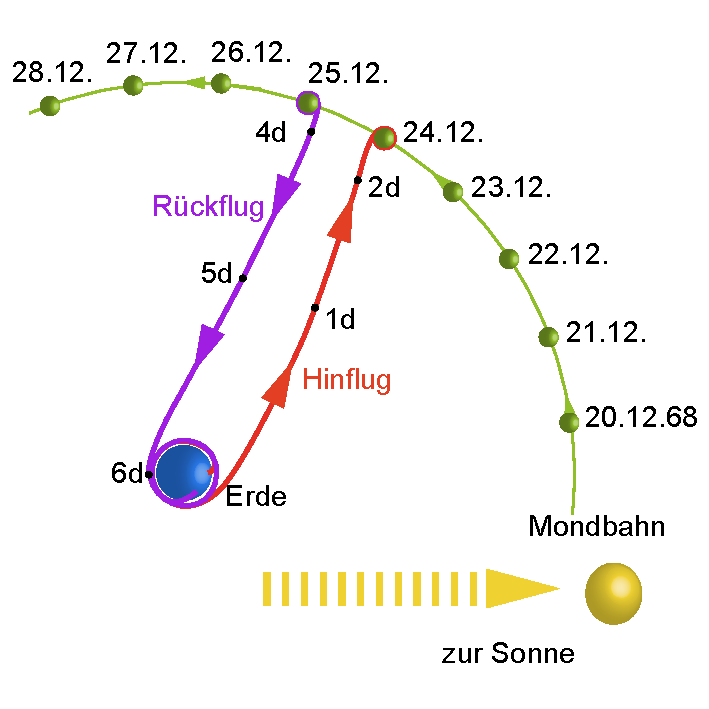
\includegraphics[width=0.5\textwidth]{Apollo8_Bahn.pdf}}
\hspace{\fill}
\rightfigure{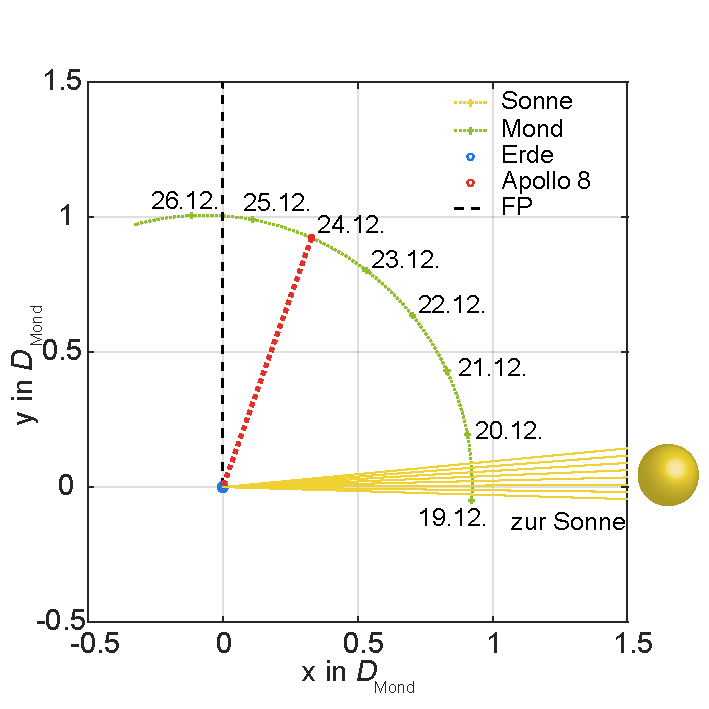
\includegraphics[width=0.5\textwidth]{KonstellationSEMA.pdf}}
\leftcaption[Bahn von Apollo 8.]{Bahn von Apollo 8. \\(Copyright NASA)}\label{abb:hm_Apollo8_Bahn}
\rightcaption[Konstellation von Sonne, Erde, Mond und Apollo 8 am 24.12.1968.]{Berechnete Konstellation von Sonne, Erde, Mond und Apollo 8 am 24.12.1968 um 16:38 UT} \label{abb:hm_EarthRise_calc}
\end{minipage}
\end{figure}
\textcolor{blue} {$\rightarrow$ zur} \probref{hm_erdaufgang_von_apollo}.\\
\noindent\rule[1ex]{\textwidth}{0.5pt} \newpage

%-----------------------------------------------------------------------------------------------------------

\begin{sol}{prob:hm_Analemma_Mars}\label{lsg:hm_Analemma_Mars} %�bung22
\textbf{Zeitgleichung und Analemmas auf anderen Planeten} \\

Wir wollen zun�chst eine sehr einfache Berechnung zeigen, die die Form der Analemmas richtig wider gibt, allerdings keine zeitliche Entwicklung zeigt, da die Kepler-Gleichung nicht gel�st wird.
Man startet dazu mit der exzentrischen Anomalie $E$ und betrachtet ein ganzes planetarisches Jahr, von dem man wei�, dass $E = 0 \ldots 360 \degree$ ist.
Mit Formel \eqref{eq:hm_nu(t)_alternativ}
\begin{equation*}
	\tan \lk \frac{\upsilon_\text{P}}{2} \rk = \sqrt{\frac{1+e_\text{P}}{1-e_\text{P}}}\,\tan\lk\frac{E}{2}\rk~
\end{equation*}
berechnet man die wahre Anomalie $\upsilon_\text{P} (E)$ des Planeten P.
Aus dieser bestimmt man �ber \eqref{eq:hm_ekl_laenge_erde1} und \eqref{eq:hm_lambda_S(T)} die L�ngen der wahren und mittleren Sonne
\begin{equation*}
L_\text{P,\astrosun} = \upsilon_\text{P} +  L_\text{P,Per}\,,~~~ L_\text{P,M} = M_\text{P} +  L_\text{P,Per} \,.
\end{equation*}
Dazu braucht man die planetozentrische L�nge des Perihels.
Das ist der Winkelabstand des Perihels vom planetaren Fr�hlingspunkt, der sich wiederum als Schnittpunkt der �quatorebene des Planeten mit der Bahnebene des Planeten ergibt.

	\begin{figure}[H]
	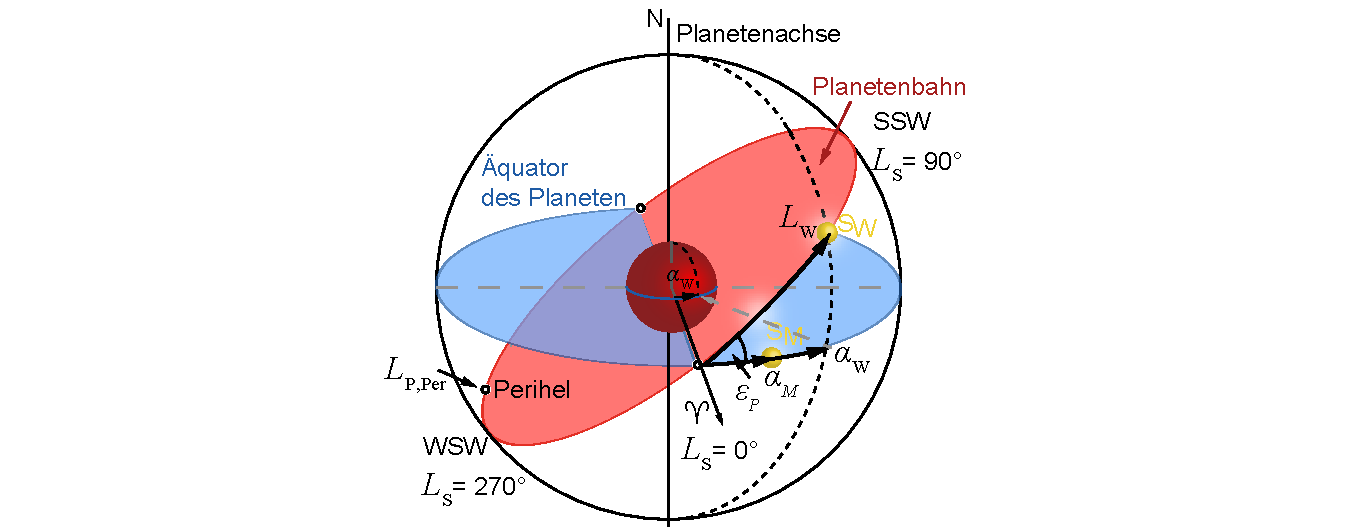
\includegraphics[width=0.8\textwidth]{ZGLGeometrie.pdf}%
	\caption{Ableitung der planetaren Sonnenkoordinaten}%
	\label{abb:hm_ZGLGeometrie_lsg}%
	\end{figure}

Wir betrachten dazu \figref{hm_ZGLGeometrie_lsg}, die der \figref{hm_wahre_sonne_geoz} aus \kap{hm_naeherungsformeln_sonne} f�r die Erde entspricht.
Wie dort dargestellt, geht es auch hier um die Anwendung von Gleichung \eqref{eq:hm_tau_ZGL_C}.
Hier m�ssen wir nun anstelle der ekliptikalen L�nge $\lambda_\text{\astrosun}$ und der geozentrischen Rektaszension $\alpha_\text{\astrosun}$ die planetozentrische L�nge $L_\text{P,\astrosun}$\index{L�nge!planetozentrische} und die planetozentrische Rektaszension \index{Rektaszension!planetozentrische} \index{Rektaszension!planetare} $\alpha_\text{P,\astrosun}$ verwenden.
Mit dem Begriff \emph{planetare} oder \emph{planetozentrische} Rektaszension ist analog zur "`normalen"' \emph{geozentrischen} Rektaszension ein Winkel gemeint, der entlang des planetaren �quators vom \emph{planetaren}(!) Fr�hlingspunkt zum Fusspunkt der wahren Sonne aus gemessen wird. 
Die (planetare) Rektaszension ergibt sich aus der entsprechenden Umrechnungsformel vom planeto-ekliptikalen System in das planeto-�quatoriale KOS (Tab. \ref{tab:hm_astro_KOS}):
\begin{equation*}
\tan\alpha_\text{P,\astrosun} = \cos\epsilon_\text{P} \, \tan{L_\text{P,\astrosun}} ~~\text{bzw.}~~~ \alpha_\text{P,M} = L_\text{P,M}~,
\end{equation*}
worin $\epsilon_\text{P}$ die Polneigung des jeweiligen Planeten relativ zu seiner Bahn ist.
Damit ergibt sich der Stundenwinkel nach \eqref{eq:hm_tau_ZGL_C} zu $\tau = \alpha_\text{M} - \alpha_\text{\astrosun}$.
Die Deklination der wahren Sonne berechnet sich ebenfalls aus Tabelle \ref{tab:hm_astro_KOS} zu:
\begin{equation*}
\sin\delta_\text{\astrosun} = \sin\epsilon_\text{P} \, \sin{L_\text{P,\astrosun}} ~, 
\end{equation*}
womit wir alle Berechnungsdaten f�r die Analemmas der Planeten haben.

\begin{figure}[H]
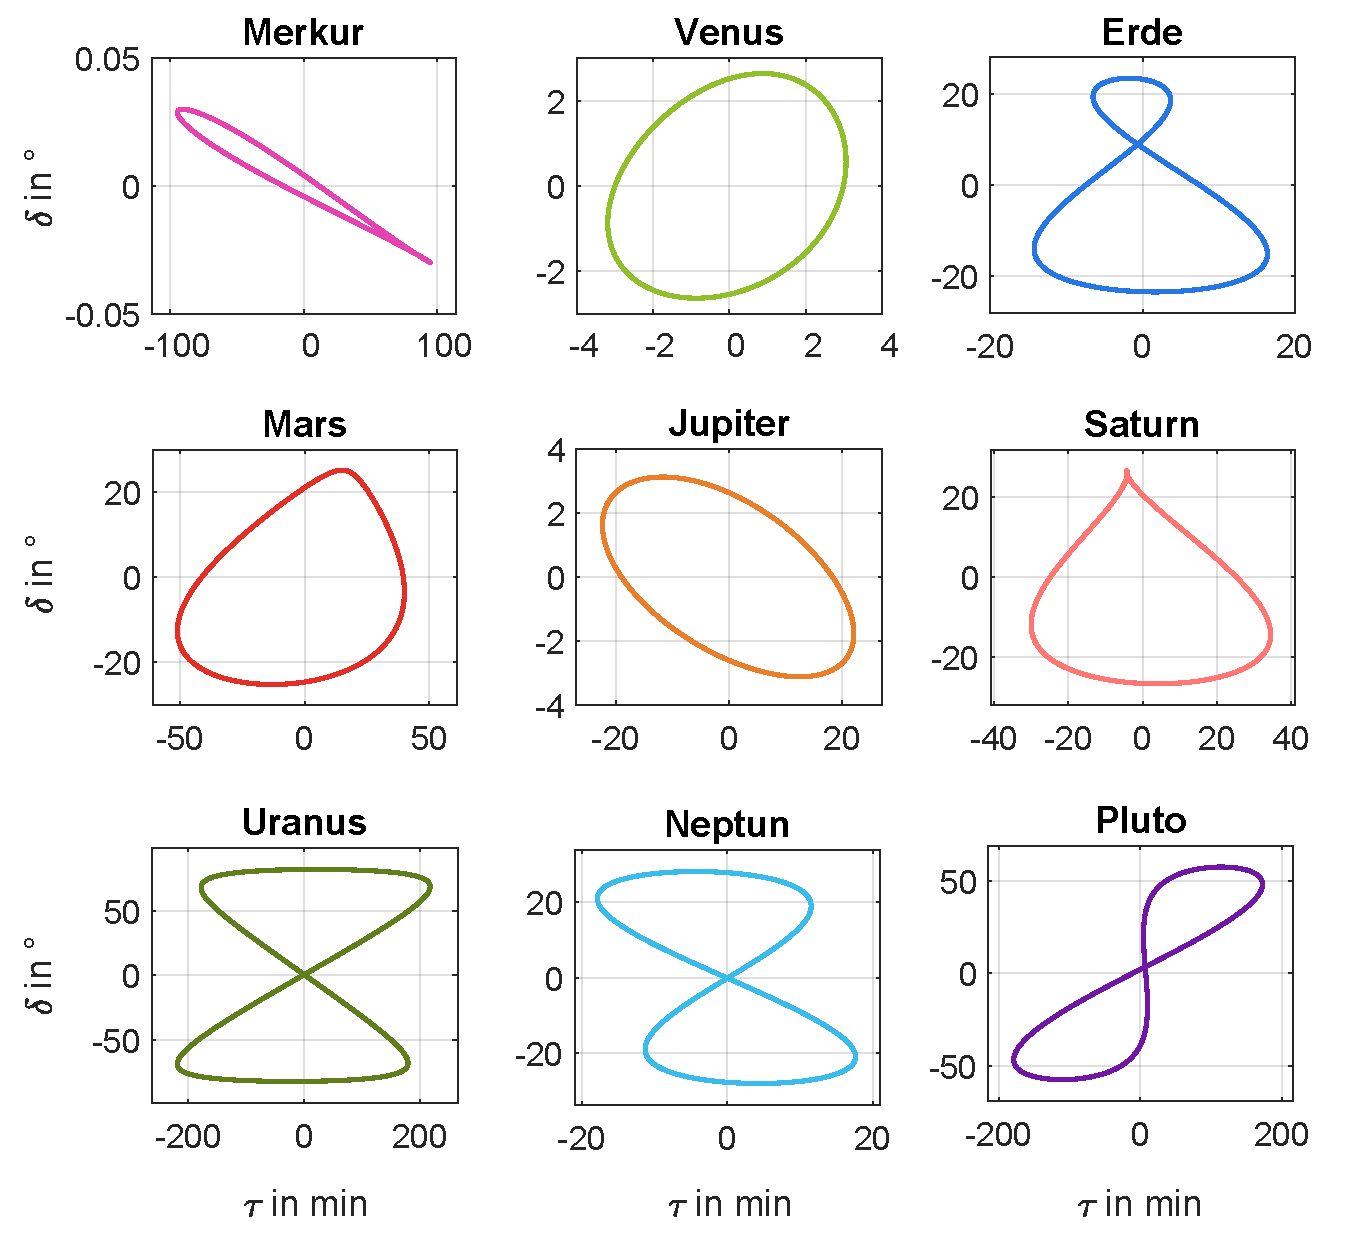
\includegraphics[width=\textwidth]{AnalemmaPlaneten.pdf}
\caption{Analemma f�r die Planeten Merkur bis Pluto.}\label{abb:hm_analemma_planeten_lsg}
\end{figure}
Details der Berechnung sind in \mlhmref{Analemma03.m} zu finden.
Das Ergebnis der Berechnung l�sst sich zusammenfassen, wobei wir den Index P f�r den Planeten weglassen, aber noch einmal darauf hinweisen, dass hier die $L_\text{Per}$ nicht den in Tabelle \ref{tab:hm_bahnparameter} gelisteten heliozentrisch-ekliptikalen L�ngen des Perihels entsprechen, sondern den planetozentrischen $L_\text{P,Per}$.
\begin{align*}
    \tau_\text{ZGL}(E) &= M + L_\text{Per} - \arctan\left\{\cos\epsilon\:\tan\left[L_\text{Per} +  2 \arctan\lk\sqrt{\frac{1+e}{1-e}} \tan\lk \frac{E}{2} \rk \rk \right] \right\} ~,\\
    \delta(E) &= \arcsin\left\{\sin\epsilon \sin\left[L_\text{Per} + 2 \arctan\lk \sqrt{\frac{1+e}{1-e}} \tan\lk \frac{E}{2} \rk \rk \right] \right\}
\end{align*}
Die entsprechenden Rechnungen haben wir im \mscr~\mlhmref{AnalemmaAnomalie.m} durchgef�hrt und sind in \figref{hm_analemma_planeten_lsg} gezeigt.
Wir geben die planetozentrischen L�ngen des Perihels ebenfalls im \mscr~an.
Wir sehen im Ergebnis, dass nur auf einigen Planeten  das Analemma als die von der Erde bekannten Figur der "`Acht"' erscheint, auf anderen Planeten kommt es wegen des unterschiedlichen Zusammenspiels der Parameter Achsneigung und Exzentrizit�t zu anderen Bildern.
Wenn einer der Bahnparameter dominiert, wie z.B. die Exzentrizit�t beim Mars, dann �hnelt das Analemma eher einer Tr�ne (siehe \figref{hm_analemma_planeten_lsg}), wenn hingegen die Achsneigung sehr klein ist, wie beim Jupiter (nur $3\degree$) wird die Figur �hnlich einer Ellipse.
Man beachte daher die ausgepr�gte Form und Breite bei Planetenbahnen mit gro�er Exzentrizit�t (Merkur, Mars, Saturn), die verschwindende Form der "`Acht"' bei geringer Polneigung (Merkur, Venus, Jupiter) bzw. das �berwiegen der Exzentrizit�t �ber die Polneigung (Mars, Saturn).\\
Wir wollen uns nun auch der Zeitgleichung zuwenden und m�ssen dazu die L�sung der Kepler-Gleichung f�r den jeweiligen Planeten ber�cksichtigen.
Wir skizzieren dazu zwei alternative Methoden. \\

\emph{Methode 1 (nach Allison\footnote{Die Rechnungen erfolgen analog den Betrachtungen in Kapitel \ref{kap:zeitgleichung} und sind in den \mscren zur �bung im Detail beschrieben. Wir verweisen ferner auf die Darstellungen in \cite{Allison2000} und \cite{Goddard2019}, in denen die Rechnungen ausf�hrlich f�r den Mars hergeleitet wurden. Wir haben in der �bung das Vorgehen f�r alle Planeten verallgemeinert.})}

Die Rotation des Planeten muss man zun�chst nicht ber�cksichtigen.
Man muss aber wiederum die Lage der Planetenbahn relativ zum planetaren �quator kennen oder m.a.W. die Richtung der Planetenrotationsachse relativ zu seiner Bahnebene.
Wir verweisen wieder auf die \figref{hm_ZGLGeometrie_lsg}, dann besteht die Aufgabe in Folgendem:
\begin{enumerate} 
	\item 	Es m�ssen die Keplerschen Elemente der Planetenbahn (bzw. der vom Planeten aus gesehenen Sonnenbahn) relativ zum planetaren �quator und Fr�hlingspunkt ausgedr�ckt werden.
          Bekannt sind dabei ja zun�chst nur die Bahnelemente bezogen auf die (Erd-)Ekliptik und den Erdfr�hlingspunkt.
          Halbachse und Exzentrizit�t �ndern sich nicht, ebenso bleibt die mittlere Anomalie unver�ndert.
          Die anderen Bahnelemente m�ssen jedoch transformiert werden.
	\item 	Mit der Inklination $i$, der L�nge des Knotens $\Omega$, dem Argument des Perihels $\omega$ und der Richtung der Rotationsachse des Planeten (deren Richtungswerte\footnote{Mit Richtung der Rotationsachse meinen wir die geozentrische Rektaszension und Deklination des Punktes an der Himmelskugel auf den die Rotationsachse zeigt.} $\alpha_0, \delta_0$ man aus der Literatur entnimmt) muss man nun die Lage des planetaren Fr�hlingspunktes (PFP) \index{Fr�hlingspunkt!planetarer} auf dem planetaren �quator berechnen (siehe \figref{hm_ZGLNullmeridian_lsg}) und daraus den Winkel $L_{\text{P,Per}}$ zwischen planetarem Fr�hlingspunkt und Perihelion der Planetenbahn.
	\item 	Am einfachsten geht das mittels Rotationsmatrizen f�r die kartesischen Vektoren normal zu den einzelnen Ebenen und entlang der jeweiligen Knotenlinien. 
	\item 	Mit diesen Gr��en kann dann die planetare Zeitgleichung, die der ekliptikalen ZGL nach \eqref{eq:hm_tau_ZGL_C} bzw. \eqref{eq:hm_tau_ZGL_C1} entspricht, berechnet werden:
		\[\tau_\text{ZGL, P} = (L_\text{P,\astrosun}-\alpha_\text{P,\astrosun}) + \mathcal{C} \\
	\]
	\item Mit der Deklination $\delta_\text{P,\astrosun}$, die wir aus der planetozentrischen L�nge der Sonne und der Achsneigung analog \eqref{eq:hm_alpha_s_delta_s} berechnen, erstellen wir dann das Analemma.
\end{enumerate}

\begin{figure}[H]
	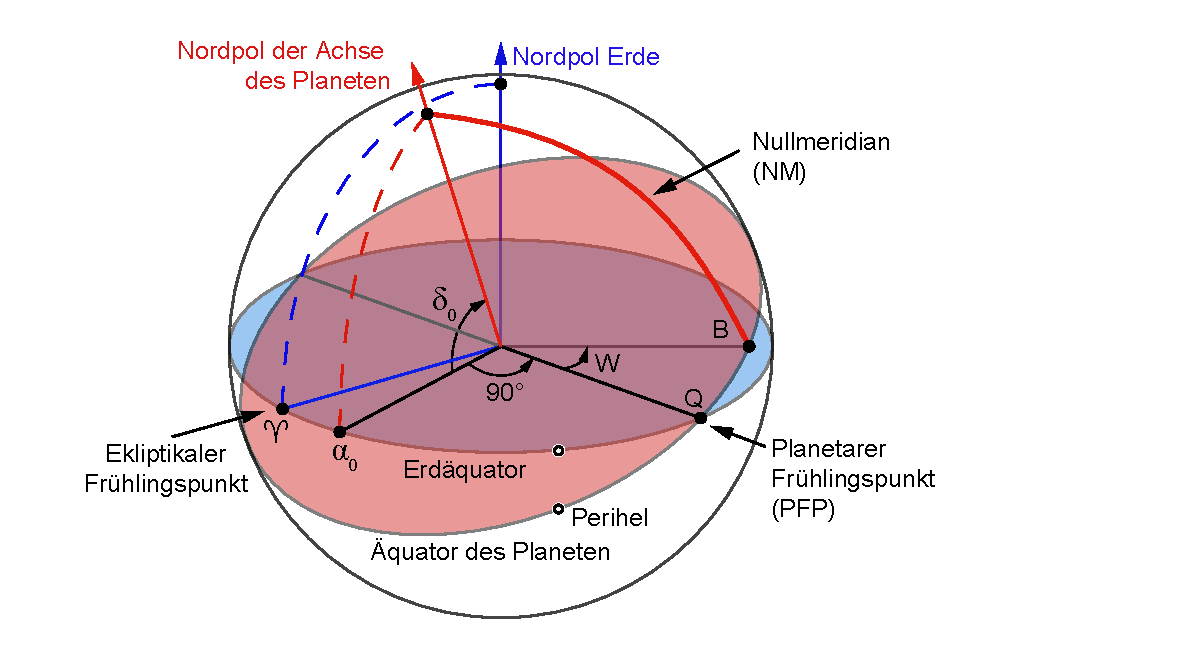
\includegraphics[width=\textwidth]{ZGLNullmeridian.pdf}%
	\caption[Planetarer Fr�hlingspunkt und Nullmeridian.]{Planetarer Fr�hlingspunkt (PFP) und Nullmeridian (NM).}%
	\label{abb:hm_ZGLNullmeridian_lsg}%
\end{figure}

Die entsprechenden Rechnungen haben wir im \mscr~\mlhmref{ZGLAnalemma.m} durchgef�hrt.

\begin{figure}[H]
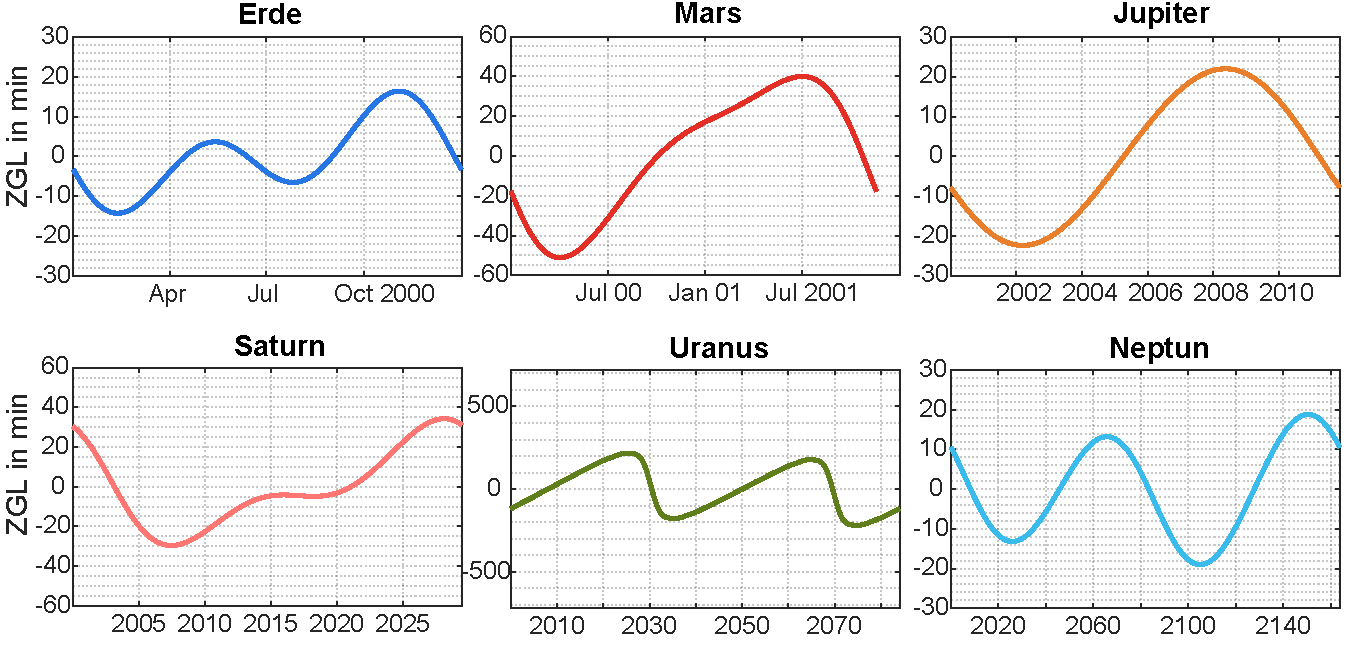
\includegraphics[width=\textwidth]{ZGLAnalemma.pdf}
\caption{Zeitgleichung f�r einige Planeten.}\label{abb:hm_zgl_planeten_lsg}
\end{figure}

Die Ergebnisse der Zeitgleichungsrechnung sind in \ref{abb:hm_zgl_planeten_lsg} dargestellt, die Analemmas stimmen erwartungsgem�� mit denen von \ref{abb:hm_analemma_planeten_lsg} �berein.
Wir wollen hier nochmals auf die Besonderheit des Uranus verweisen.
Der Uranus braucht etwa 84 Jahre, bis er die Sonne einmal umrundet hat.
Dabei dauert ein Tag auf dem Uranus nur 17 Stunden und 14 Minuten.
Da seine Polachse fast in der Bahnebene liegt rollt er quasi auf seiner Bahnebene um die Sonne, wobei f�r fast ein halbes Jahr der Nordpol, das andere Halbjahr der S�dpol zur Sonne zeigt.
Die ZGL und damit Jahreszeiten sind aus diesem Grund ziemlich "`verr�ckt"'.
Es bleibt auf dem Uranus im Sommer 42 Erden-Jahre lang st�ndig hell und wird dann abrupt dunkel.
Das Analemma zeigt das sehr sch�n.\\

\emph{Methode 2 (nach Montenbruck\footnote{Mit der Methode ist dann auch die Position jedes anderen Himmelsk�rpers im KOS des Planeten berechenbar. F�r Details verweisen wir auf \cite{Montenbruck1999, Haase2013}.})} 

Auch hier wollen wir die Methodik kurz skizzieren.
Man berechnet (numerisch) f�r einen Punkt auf der Oberfl�che des Planeten (gegeben durch die planetographischen Koordinaten $\varphi_\text{P}$ und $\lambda_\text{P}$) die planetare Rektaszension und Deklination der Sonne im planetozentrischem �quatorialsystem f�r den Verlauf eines tropischen Jahres.
Aus diesen Koordinaten lassen sich dann v�llig analog zur Erde bei Festlegung einer geeigneten Planeten-Nullzeit (z.B. Nullmeridian NM in \figref{hm_ZGLNullmeridian_lsg}) die Aufg�nge und Unterg�nge der Sonne und nat�rlich auch den Meridiandurchgang f�r jeden Ort $\varphi_\text{P}$, $\lambda_\text{P}$ des Planeten bestimmen.
Zusammengefasst ist das Vorgehen also wie folgt:
\begin{enumerate} 
	\item Ausgehend von der heliozentrischen Position des Planeten berechnet man die planetozentrischen Koordinaten $\alpha_\text{P,\astrosun}$  und $\delta_\text{P,\astrosun}$ der wahren Sonne im Verlauf eines tropischen Jahres.
	\item Die mittlere Sonne berechnen wir �ber die mittlere Anomalie.
          Alternativ k�nnten wir auch aus der Kenntnis der Rotationsperiode des Planeten eine Planetensternzeit $\theta_\text{P}$ berechnen, wobei sich die Zeitgleichung dann entweder �ber \eqref{eq:hm_tau_ZGL_C} bzw. $\tau_\text{ZGL} = \theta_\text{P} - \alpha_\text{P,\astrosun}$ berechnet. 
	\item Mit der Deklination $\delta_\text{P,\astrosun}$ aus der planetozentrischen Breite der wahren Sonne erstellen wir dann das Analemma.
\end{enumerate}

Die entsprechenden Rechnungen haben wir im \mscr~\mlhmref{ZGLAnalemmaKepler.m} bzw. f�r alle Planeten hinterlegt.
Auch hier stimmen die Analemmas erwartungsgem�� mit denen von \figref{hm_analemma_planeten_lsg} und die Zeitgleichungen mit denen von \figref{hm_zgl_planeten_lsg} �berein. \\

Eine sch�ne Erweiterung der Methodik ist die Anwendung auf die Berechnung eines Analemmas des Mondes (von der Erde aus betrachtet) \bzw eines Analemmas der Sonne vom Mond aus betrachtet.
In den \matlab{}-Skripten \mlhmref{ZGLAnalemma.m}, \mlhmref{ZGLAnalemmaKepler.m} und \mlhmref{AnalemmaAnomalie.m} sind die Rechnungen dazu detailliert hinterlegt.

\medskip \end{sol}
\textcolor{blue} {$\rightarrow$ zur} \probref{hm_Analemma_Mars}.\\
\noindent\rule[1ex]{\textwidth}{0.5pt} \newpage

%-----------------------------------------------------------------------------------------------------------

\begin{sol}{prob:hm_sonnenaufgang_mars}\label{lsg:hm_sonnenaufgang_mars} %�bung23
\textbf{Sonnenaufgang Mars} \\ \\
In \probref{hm_Analemma_Mars} haben wir die Zeitgleichung und das Analemma f�r den Mars hergeleitet.
Wir haben dort ebenfalls eine Referenz f�r die Zeitmessung auf den Mars und einen Bezug zur UTC hergestellt.
Wir k�nnen selbstverst�ndlich auch andere Referenzzeitpunkte w�hlen, wie \zb die Landezeit einer Marssonde. 
Wir wollen nun auf Basis der aktuellen NASA Konventionen die Sonnenaufgangsberechnung durchf�hren und benutzen dabei neben den Ergebnissen von \probref{hm_Analemma_Mars} auch den Algorithmus der NASA \cite{Goddard2019}.
Die detaillierten Rechnungen sind i\mscr{} \mlhmref{OlympusMons.m} hinterlegt, das Ergebnis der Rechnungen ist in \figref{hm_Mars_Sunrise_lsg} zu sehen.
Wie schon beim Analemma in L�sung \ref{lsg:hm_Analemma_Mars} erkennt man auch hier deutlich die unterschiedlich langen Jahreszeiten (als Folge der gro�en Exzentrizit�t) und auch, da der Beobachtungsort nahe des Mars-�quators liegt, dass die jahreszeitlichen Schwankungen im wesentlichen die ZGL widerspiegeln.\\
\begin{figure}[H]
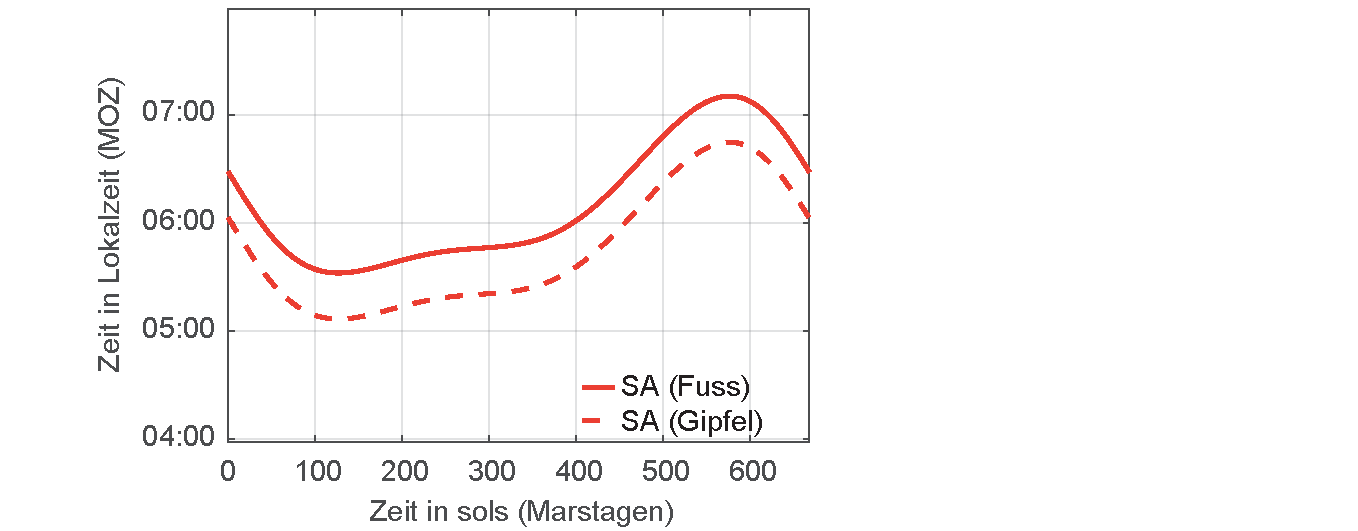
\includegraphics[width=\columnwidth]{OlympusMons.pdf}%
\caption[Sonnenaufgangszeiten auf dem Mars.]{Sonnenaufgangszeiten auf dem Mars am Fu� und auf dem Gipfel des Olympus Mons im Verlauf eines Mars-Jahres. Das Mars-Sommer Halbjahr erstreckt etwa von Tag 1 bis Tag 450 und damit wesentlich l�nger als das Winterhalbjahr.}%
\label{abb:hm_Mars_Sunrise_lsg}%
\end{figure}
\medskip \end{sol}
\textcolor{blue} {$\rightarrow$ zur} \probref{hm_sonnenaufgang_mars}.\\
\noindent\rule[1ex]{\textwidth}{0.5pt} \newpage

%-----------------------------------------------------------------------------------------------------------
\newpage
%%%-----------------------------------------------------------------------------------------------------------
\subsection{�bungen zu Monden, Kometen und Asteroiden}

\medskip

\begin{sol}{prob:hm_MondbahnHelioz}\label{lsg:hm_MondbahnHelioz} %�bung24
\textbf{Heliozentrische Mondbahn} \\

Heliozentrisch betrachtet l�uft der Mond um die Sonne und wird dabei von der Erde ein wenig abgelenkt. Die Mondbahn ist aber stets
zur Sonne hin gekr�mmt, und die St�rke dieser Kr�mmung �ndert
sich im Lauf eines Monats nur m��ig, da die Gravitationskraft
der Sonne am Ort des Mondes zu jeder Zeit deutlich
gr��er als diejenige der Erde ist, was man leicht nachrechnen kann. 
Geozentrisch ist es aber ebenfalls richtig zu sagen,
dass der Mond um die Erde l�uft und dabei von der Sonne
gest�rt wird, was zu seiner komplexen Bahn f�hrt.
Es gilt aber auch hier, dass die Schwerkraft
der Erde am Ort des Mondes zu jedem Zeitpunkt deutlich gr��er ist als
die Gezeitenkraft der Sonne auf das Erde-Mond-System ist, denn sonst w�rde dieses ja auseinander gerissen werden (siehe \kap{hm_gezeiten}). Man kann auch sagen, dass nur die Differenz der solaren Einfl�sse auf Erde und Mond sich als St�rung der
geozentrischen Mondbahn auswirkt.\\
Man kann sich nun recht einfach �berlegen, unter welchen Bedingungen schleifen- oder wellenf�rmige Mondbahnen zustande kommen k�nnen.
Wir wollen vereinfachend annehmen, dass die Planetenbahn und zugeh�rige Mondbahn ann�hernd koplanar und zirkular sind, also
gegeneinander nur wenig geneigt und wenig exzentrisch sind. 
Aus der Gravitationsbeschleunigung und dem dritten Keplerschen Gesetz findet man
folgende Beziehungen:
\begin{itemize}
\item Fall 1: Konvexe Bahn (wie Erdmond) : $T_\text{M}^2/T_\text{P}^2 > a_\text{M}/a_\text{P}$
\item Fall 2: Schleifenbahn : $T_\text{M}/T_\text{P} < a_\text{M}/a_\text{P}$
\item Fall 3: Wellenbahn : $T_\text{M}/T_\text{P} > a_\text{M}/a_\text{P} > T_\text{M}^2/T_\text{P}^2$
\end{itemize}
Hierin sind $T_\text{M},\, T_\text{P}$ die Umlaufzeiten von Mond und Planet und $a_\text{M},\, a_\text{P}$ die entsprechenden Radien der Bahnen.
Die erste Bedingung besagt, dass die
Gravitationsbeschleunigung des Mondes
durch den Planeten kleiner ist als diejenige
durch die Sonne, was beim Erdmond sicher erf�llt ist. Die zweite Bedingung
besagt, dass die Umlaufgeschwindigkeit
des Mondes um den Planeten gr��er
ist als die Geschwindigkeit des Planeten
um die Sonne. Dies ist beim Erde Mond System nicht erf�llt. Wegen $a_\text{M} \ll a_\text{P}$ ergibt sich deshalb beim Mond der Erde nur eine geringf�gig ausgepr�gte Wellenbahn 
(\figref{hm_mondbahn_lsg02}).\\
Wir wollen das in einer einfachen, komplanaren Modellrechnung zeigen und schreiben: 
\begin{align}
\begin{split}
    x_\text{M} &= a_\text{P}\,\cos\Omega_\text{P} \,t + a_\text{M}\,\cos\omega_\text{M}\,t \\
    y_\text{M} &= a_\text{P}\,\sin\Omega_\text{P} \,t + a_\text{M}\,\sin\omega_\text{M}\,t
\end{split} \label{eq:hm_lsgmondb01}
\end{align}
$t=0$ wurde hier so gew�hlt, dass $\vec{r}\lk 0\rk = \vec{r}_\text{M,0}  =  \lk x_\text{M},y_\text{M} \rk= \lk a_\text{P} + a_\text{M},0\rk $ ist. \\
Unser Kurvenparameter ist die Zeit $t$. Wir wollen den Kr�mmungsradius $\varrho$ und die Konvexit�t $\eta = \D^2 y/\D x^2$ als Funktion der Zeit berechnen. Gilt $\eta > 0$ ist die Bahn konvex, f�r Zeitbereiche in denen $\eta <0$ ist die Bahn konkav. \\
In Parameterdarstellung ist der Kr�mmungsradius $\varrho$ gegeben durch:
\begin{align}
    \varrho = \Bigg|\frac{\lk \dot{x}^2+ \dot{y}^2\rk^\frac{3}{2}}{\lk \dot{x}\ddot{y} -\ddot{x}\dot{y}\rk}\Bigg| = \Bigg|\frac{\lk \dot{x}^2+ \dot{y}^2\rk^\frac{3}{2}}{\det\lk \dot{\vec{r}},\ddot{\vec{r}}\rk}\Bigg| \label{eq:hm_lsgmondb02} \,. 
\end{align}
\begin{table}[h!]
    \centering
    \begin{tabular}{l|rcrcr}
         & $T_\text{M}{}^2/T_\text{P}{}^2$ & & $a_\text{M}/a_\text{P}$&&$T_\text{M}/T_\text{P}$\\
         \rule{0pt}{1pt}& & & & &  \\
         \hline
         \rule{0pt}{1pt}& & & & &  \\
         \rule{0pt}{6pt}Fall 1~~~ & $~0.25$ & $>$ & $0.1$ & & $0.5$ \\
         \rule{0pt}{6pt}Fall 2~~~ & $~0.0025$ & & $0.1$ & $>$& $0.05$ \\
         \rule{0pt}{6pt}Fall 3~~~ & $~0.01$ & $<$ & $0.1$ & $\leq$& $0.1$ 
    \end{tabular}
\end{table}\\
Man erkennt deutlich, dass je nach Fall die Schleifenbahn, eine Art Epizykloide auf einem Kreis mit dem Radius $a_\text{P}-a_\text{M}$ oder eben eine sehr flache Welle darstellt. Das Erde-Mond System f�llt in die Kategorie des Fall 1 mit $a_\text{P} \gg a_\text{M}$.\\
F�r stark geneigte Bahnen ergben sich durch notwendige Ber�cksichtigung der Bahnneigung etwas durch die Inklination
$\cos i$ modifizierte Beziehungen.\\
Die numerische Berechnung der 3 Beispiele ist mit entsprechenden Modellparametern sehr einfach zu realisieren und im \mscr{} \mlhmref{Mondbahn01.m} f�r koplanare kreisf�rmige Bahnen ausgef�hrt. Im \mscr{} \mlhmref{Mondbahn02.m} ist auch die heliozentrische Mondbahn aus den genauen Ephemeriden berechnet (\figref{hm_mondbahn_lsg03}).

\begin{figure}[H]
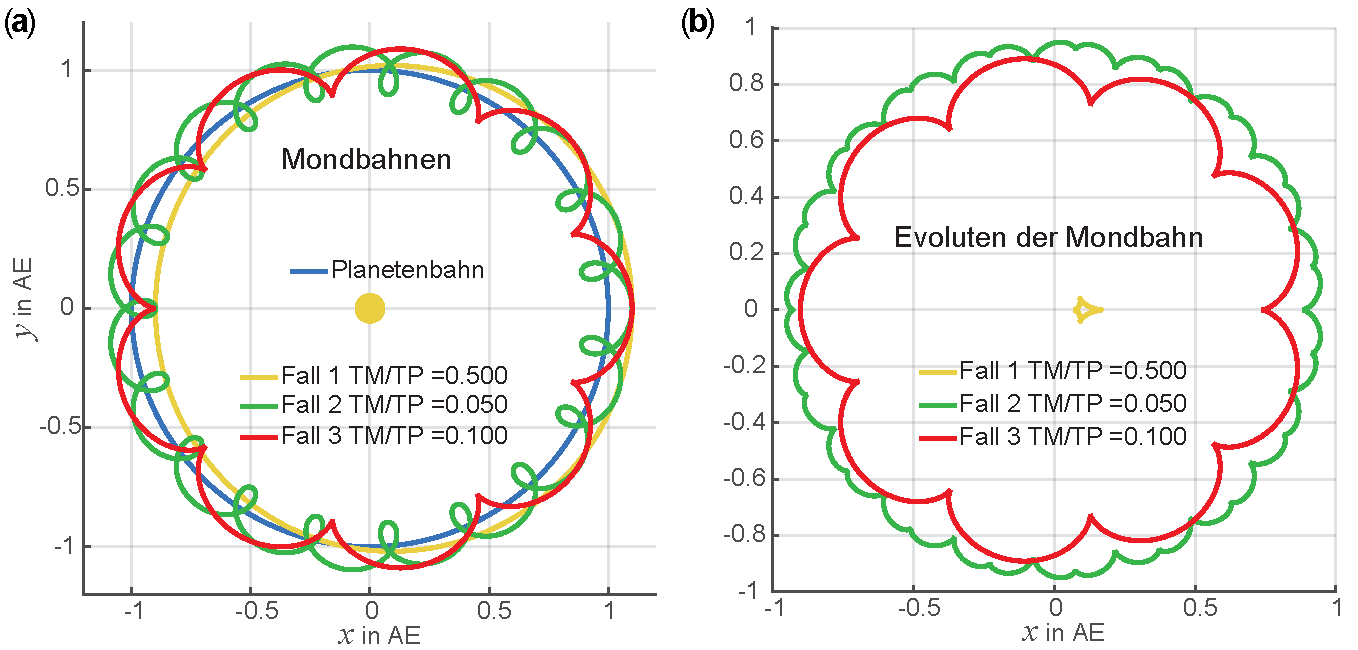
\includegraphics[width=\textwidth]{MondbahnHelioz3.pdf}
\caption[Heliozentrische Mondbahnen f�r koplanare, kreisf�rmige Bahnen.]{Heliozentrische Mondbahnen f�r koplanare, kreisf�rmige Bahnen Planet und Mond. \fa Mondbahnen \fb Lage der Mittelpunkte des lokalen Kr�mmungskreises (Evolute der Mondbahn). Das Verh�ltnis der Bahnradien von Mondbahn zu Planetenbahn wurde fest zu 0.1 angenommen, variiert wurden die Umlaufzeiten \bzw nach dem 3. Keplerschen Gesetz die Massen von Zentralk�rper und Planet.}\label{abb:hm_mondbahn_lsg01}
\end{figure}

\begin{figure}[H]
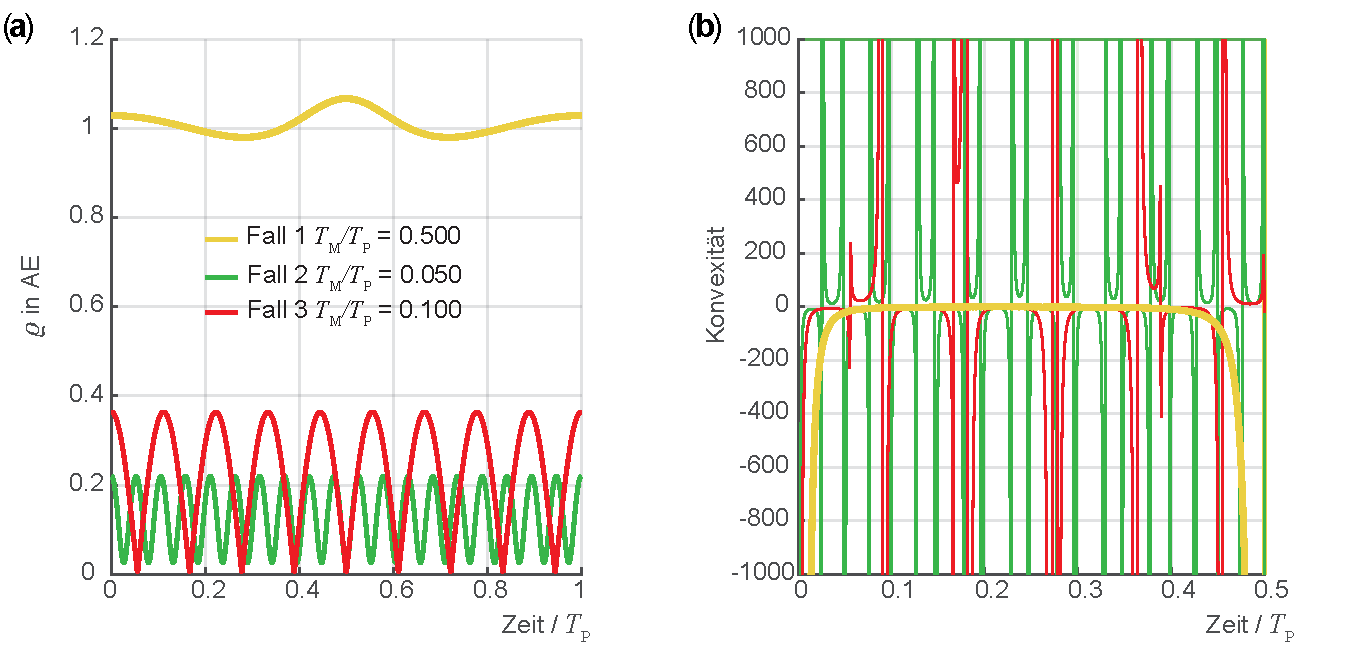
\includegraphics[width=\textwidth]{MondbahnHelioz4.pdf}
\caption[Kr�mmungsradius und Konvexit�t heliozentrischer Mondbahnen.]{Heliozentrische Mondbahnen f�r koplanare, kreisf�rmige Bahnen Planet und Mond. \fa Kr�mmungsradius \fb Konvexit�t. Das Verh�ltnis der Bahnradien von Mondbahn zu Planetenbahn wurde fest zu 0.1 angenommen, variiert wurden die Umlaufzeiten \bzw nach dem 3. Keplerschen Gesetz die Massen von Zentralk�rper und Planet.}\label{abb:hm_mondbahn_lsg02}
\end{figure}

\begin{figure}[H]
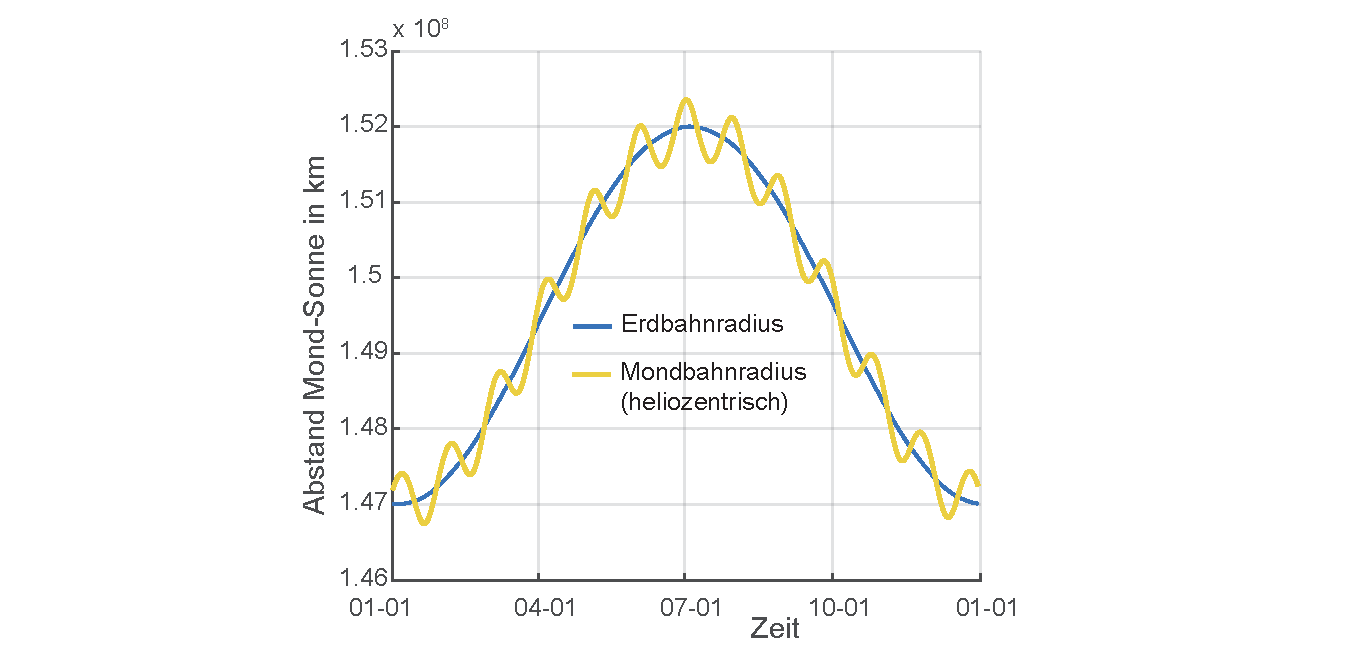
\includegraphics[width=\textwidth]{MondbahnHelioz2.pdf}
\caption{Heliozentrische Mondbahn aus den Ephemeriden berechnet}\label{abb:hm_mondbahn_lsg03}
\end{figure}


\medskip \end{sol}
\textcolor{blue} {$\rightarrow$ zur} \probref{hm_MondbahnHelioz}.\\
\noindent\rule[1ex]{\textwidth}{0.5pt} \newpage



%-----------------------------------------------------------------------------------------------------------

\begin{sol}{prob:hm_kometen_asteroiden} \label{lsg:hm_kometen_asteroiden} %�bung25
\textbf{Kometen und Asteroiden} \\ \\
Die Rechnungen sind im Detail in den einzelnen \mscren zu den Kometen- und Asteroidenbahnen \ua \mlhmref{AsteroidenBahnen.m} und \mlhmref{AsteroidenZeit.m} ausgef�hrt. Eine Beispielrechnung ist als Bild angef�gt. \\

\begin{figure}[H]
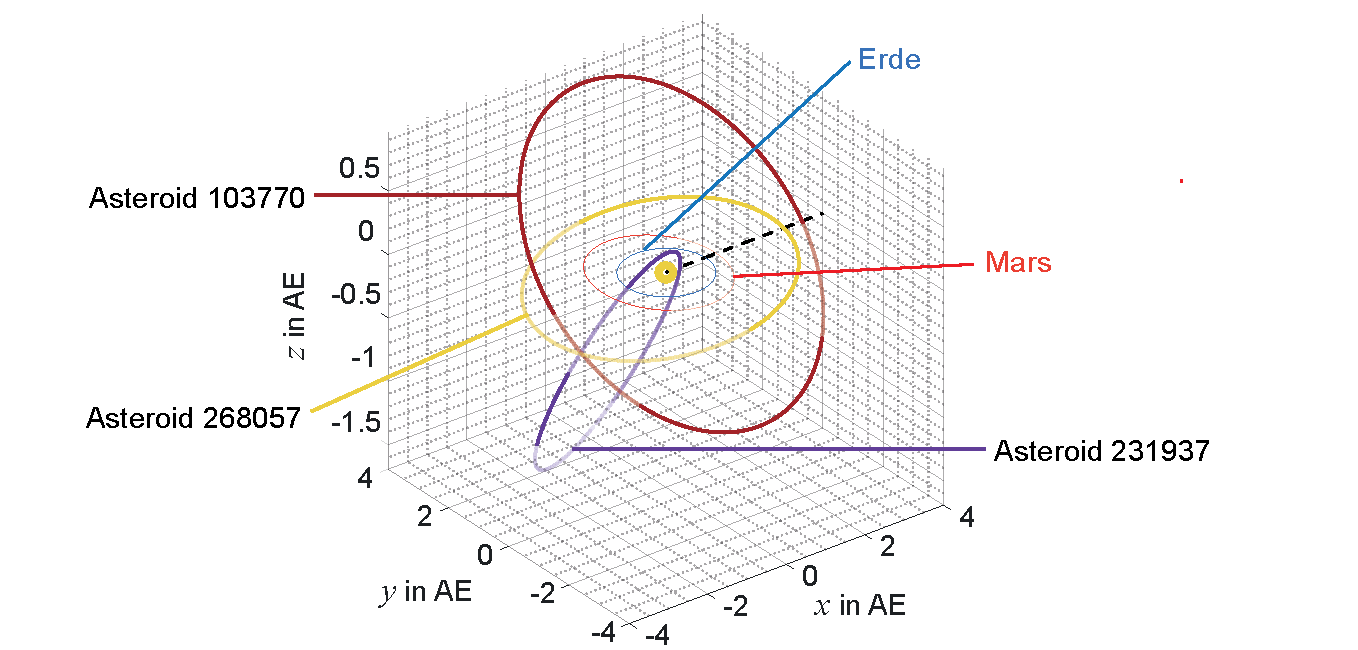
\includegraphics[width=\textwidth]{AsteroidenbahnenBeispiele.pdf}
\caption{Beispiele vo Asteroidenbahnen}\label{abb:hm_AsteroidenbahnenBeispiele}
\end{figure}

\medskip \end{sol}
\textcolor{blue} {$\rightarrow$ zur} \probref{hm_kometen_asteroiden}.\\
\noindent\rule[1ex]{\textwidth}{0.5pt} \newpage


%-----------------------------------------------------------------------------------------------------------


\begin{sol}{prob:hm_verweildauer_komet_erdbahn}\label{lsg:hm_verweildauer_komet_erdbahn} %�bung26
\textbf{Kometen und Meteoriten} \\
\begin{enumerate}[(a)]
	\item Wir vereinfachen zun�chst das Problem und nehmen an, dass die Kometenbahn in der Ekliptik liegt und dass diese in der N�he ihres Perihels als Parabel beschrieben werden kann.
          Somit ist die Exzentrizit�t $e\!=\!1$ und \eqref{eq:hm_kegelschnitt} vereinfacht sich zu
\begin{equation}
r = \frac{p}{1+\cos\upsilon}~~\text{mit}~~p=\frac{L^2}{\mu_\text{G}} ~~.\label{eq:hm_hmlsg_24_1}
\end{equation}
Der minimale Abstand ist demnach $r_\text{min}\!=\!q\!=\!p/2\!=\!L^2/(2\mu_\text{G})$.
F�r die spezifische Energie des Kometen gilt nach \eqref{eq:hm_total_energy} im Fall von Parabeln
\begin{equation}
H = \frac{1}{2}\dot{r}^2 + \frac{L^2}{2r^2} + U(r) ~~. \label{eq:hm_hmlsg_24_2}
\end{equation}
Am Perihel mit Abstand $r_\text{min} = q$ ist die Radialgeschwindigkeit $\dot{r}\!=\!0$, so dass
\begin{align*}
	\frac{L^2}{2r_\text{min}^2} &= -U(r_\text{min}) = \frac{\mu_\text{G}}{r_\text{min}} = \frac{\mu_\text{G}}{q} \\
	\Rightarrow L &= \sqrt{2\mu_\text{G}\,q}~~.
\end{align*}
Wir dr�cken nun den Perihelabstand als $q\!=\!r_\text{min}\!=\!ka_\text{\earth}\!=\! k\, 1\text{AE}$ mit $0\!<\!k\!<\!1$ aus.
Mit $\D t\!=\!\D r/\dot{r}$ und $\dot{r}\!=\!\sqrt{2[-U(r)-L^2/(2r^2)]}$ folgt aus \eqref{eq:hm_hmlsg_24_2}
\begin{align*}
	t-t_0 &= \int\limits_{q}^{r=a_\text{\earth}} \frac{r}{\sqrt{2\mu_\text{G}r-L^2}}\,\D r = \sqrt{\frac{1}{2\mu_\text{G}}} \int\limits_{q}^{r} \frac{r}{\sqrt{r-L^2/2\mu_\text{G}}}\,\D r ~~.\\
\end{align*}
In Integraltafeln finden wir als L�sung f�r das Integral
\begin{equation*}
t-t_0 = \frac{1}{\sqrt{2\mu_\text{G}}}\,\frac{2}{3}\,\sqrt{r-q}\,(2q+r) \bigg|^{a_\text{\earth}}_{q}~~.
\end{equation*}
Die Gesamtaufenthaltsdauer des Kometen innerhalb der Erdbahn, in welcher der Komet gut beobachtet werden kann, ist dann gegeben durch
\begin{align}
	T_\text{ges} &= \frac{2}{\sqrt{2\mu_\text{G}}}\,\frac{2}{3}\,\lek \sqrt{a_\text{\earth}-ka_\text{\earth}} \lk 2ka_\text{\earth} + a_\text{\earth} \rk - \sqrt{q-q} \lk 2ka_\text{\earth} + a_\text{\earth} \rk \rek \\
	 &= \frac{2}{\sqrt{2\mu_\text{G}}}\,\frac{2}{3}\,\sqrt{a_\text{\earth}^3}\,\sqrt{1-k}\,(2k+1) = \frac{4}{3}\,\sqrt{\frac{a_\text{\earth}^3}{2\mu_\text{G}}}\,\sqrt{1+3k-4k^3}~~. \label{eq:hm_verweildauer01}
\end{align}
\begin{figure}[H]
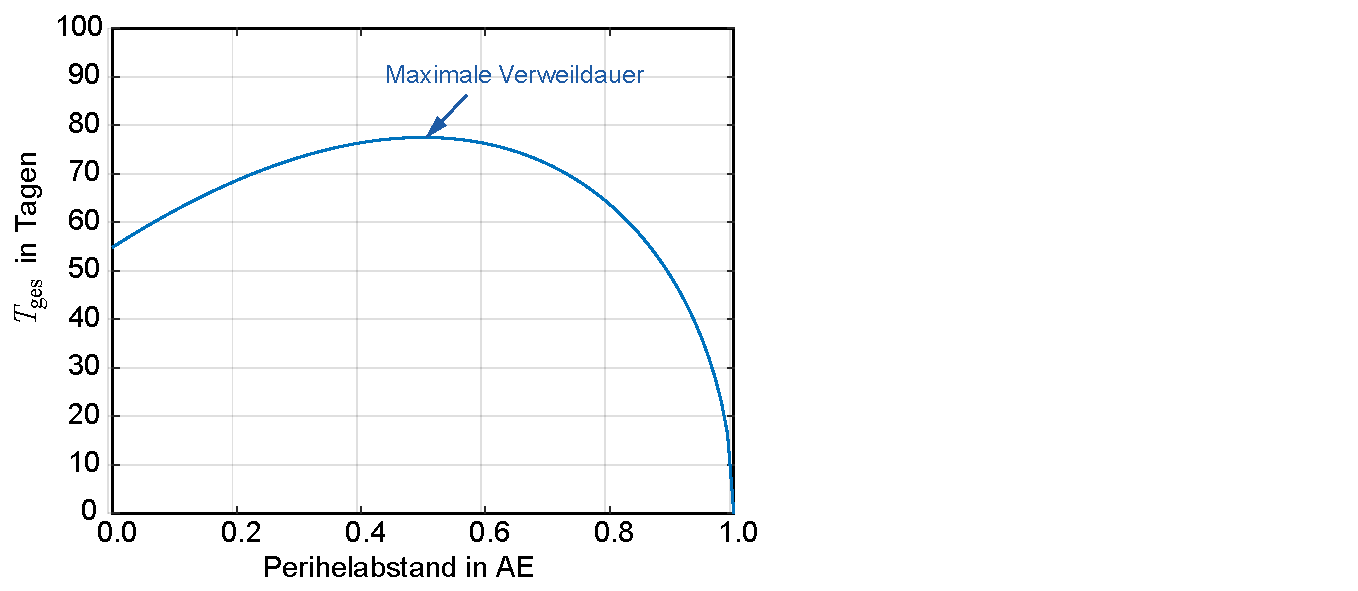
\includegraphics[width=\textwidth]{Verweildauer.pdf}%
\caption[Verweildauer des Kometen in Tagen innerhalb der Erdumlaufbahn.]{Verweildauer des Kometen in Tagen innerhalb der Erdumlaufbahn (Kriterium f�r gute Sichtbarkeit).}%
\label{abb:hm_aufenthaltsdauer_lsg}%
\end{figure}
Die \figref{hm_aufenthaltsdauer_lsg} zeigt die Verweildauer normiert auf die Umlaufdauer der Erde gem��
\begin{equation}
\frac{T_\text{ges}}{2\pi\sqrt{a_\text{\earth}^3/\mu_\text{G}}} = \frac{2}{3}\frac{1}{\sqrt{2}\pi}\,\sqrt{1+3k-4k^3}~~.\label{eq:hm_verweildauer02}
\end{equation}
Man erkennt, dass je kleiner der Perihelabstand ist, desto h�her wird die Geschwindigkeit des Kometen und desto k�rzer seine Aufenthaltsdauer innerhalb der Erdbahn, desto heller leuchtet er aber auch.
Interessant ist auch, dass die maximale Dauer auf etwa 80 Tage begrenzt ist.\\

\item Wir betrachten einen Meteoroiden, der sich im Schwerefeld von Sonne und Erde bewegt (\figref{hm_aufschlaggeschw}):
Wir wollen seine Position zun�chst in einem rotierenden KOS betrachten, das sich mit der Winkelgeschwindigkeit $\omega$ der Erde um Sonne mitdreht (\vgl dazu auch die Darstellungen in  Kap 1.2.3.6  in Band I).
Die spezifische Energie des Himmelsk�rpers im Abstand $r_\text{K}$ mit der Geschwindigkeit $v_\text{K}$ ist dann gegeben durch (wir lassen die Striche f�r das mitbewegte \KOS{} weg, der Index K steht f�r den Kometen im mitbewegten System):
\begin{equation}
 H_\text{K} = \frac{v_\text{K}^2}{2} - \frac{\mu_\text{G}m_\text{\earth}}{r_\text{K} m_\text{\astrosun}} - \frac{\mu_\text{G}}{r_\text{SK}} - \frac{\omega^2}{2}\,(x_\text{K}{}^2 + y_\text{K}{}^2)~~,
\label{eq:hm_hmlsg_24b_1}
\end{equation}
worin $\omega\!=\!\sqrt{\mu_\text{G}/a_\text{\earth}^3}$ gem�� \eqref{eq:hm_1-ecosEdE} ist, der zweite und dritte Term die potentielle Energie bzgl. der Erde und der Sonne repr�sentieren und der letzte Term das Zentrifugalpotential, hervorgerufen durch das rotierende KOS, darstellt.
Wir setzen $\alpha\!=\!m_\text{\earth}/m_\text{\astrosun}$. 

\begin{figure}[H]
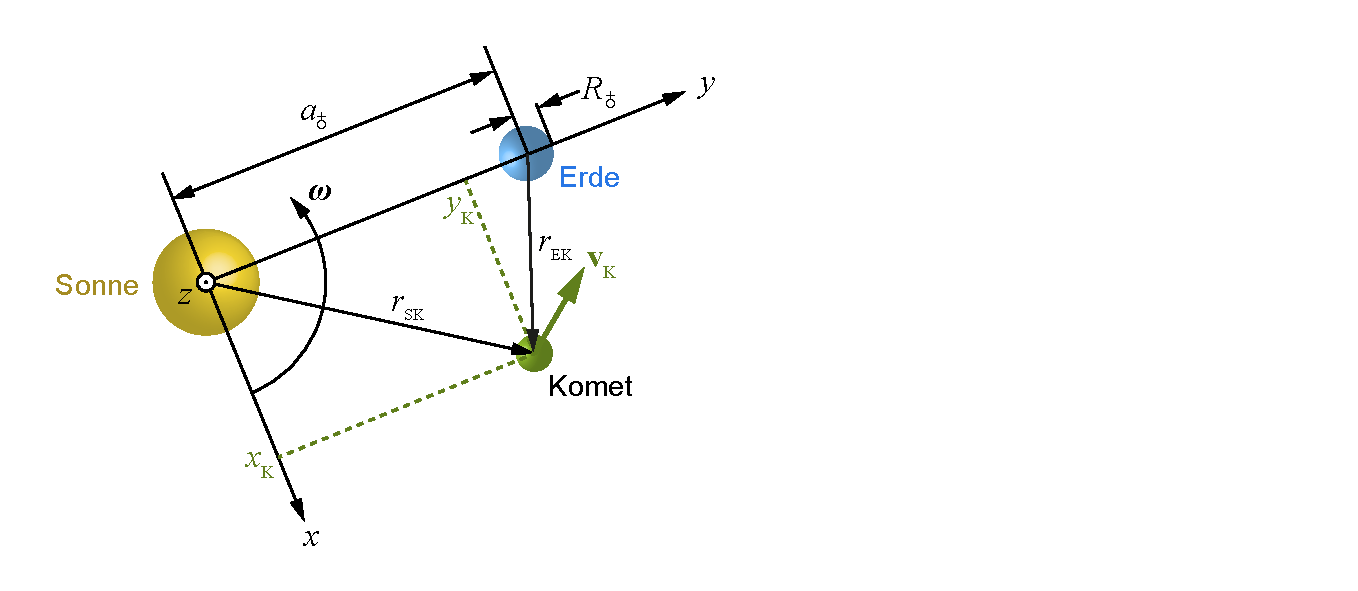
\includegraphics[width=\textwidth]{AufprallKomet.pdf}%
\caption{Zur Berechnung der Aufschlaggeschwindigkeit eines Kometen}%
\label{abb:hm_aufschlaggeschw}%
\end{figure}

F�r den Moment des Aufschlags gilt:
\begin{align}
H_\text{K,A} (r_\text{K}=R_\text{\earth}) &= \frac{v_\text{A}^2}{2} - \frac{\alpha \mu_\text{G}}{R_\text{\earth}} - \frac{\mu_\text{G}}{a_\text{\earth}} - \frac{\omega^2}{2}\,a_\text{\earth}^2 
= \frac{v_\text{A}^2}{2} - \frac{\alpha \mu_\text{G}}{R_\text{\earth}} - \frac{3\mu_\text{G}}{2a_\text{\earth}} ~~. \label{eq:hm_hmlsg_24b_2} 
\end{align}
F�r eine initiale Position mit $r_0\!\gg\! a_\text{\earth}$ k�nnen wir wegen $\alpha\!\gg\! 1$ in \eqref{eq:hm_hmlsg_24b_1} den zweiten Term vernachl�ssigen und erhalten
\begin{equation}
H_{\text{K},0} = \frac{v_0{}^{2}}{2} - \frac{\mu_\text{G}}{r_0} - \frac{\omega^2}{2}\,(x_0{}^{2} + y_0{}^{2}) ~~. 
\end{equation}
Jetzt verlassen wir das rotierende KOS und gehen in das in der Sonne verankerte Inertialsystem �ber. \label{eq:hm_hmlsg_24b_2a} 
Dann gilt f�r die Geschwindigkeit des Himmelsk�rpers in diesem KOS (man beachte die Richtung von $\vec{\omega}$):
\begin{equation}
\vec{v}_0 = \vec{v}_\text{S} - \vec{\omega}\times\vec{r}_\text{S} ~~,\label{eq:hm_hmlsg_24b_3}
\end{equation}
wobei die Indizes S die Gr��en im Inertialsystem der Sonne kennzeichnen. 
Wir k�nnen dann schreiben:
\begin{equation}
v_0{}^2 = v_\text{S}{}^{2} - 2\,\vec{v}_\text{S}(\vec{\omega}\times\vec{r}_\text{S}) + \omega^2({x_\text{S}}^2 + {y_\text{S}}^2) ~~.
\label{eq:hm_hmlsg_24b_4}
\end{equation}
Wir setzen \eqref{eq:hm_hmlsg_24b_4} in \eqref{eq:hm_hmlsg_24b_3} ein und ber�cksichtigen, dass gilt:
\begin{align*}
\vec{r}_0{}^2 &= {x_0}^{2} + {y_0}^{2} = {x_\text{S}}^{2} + {y_\text{S}}^{2} = {\vec{r}_\text{S}}^2 ~~~\text{und} ~~~ \vec{v}_\text{S}(\vec{\omega}\times\vec{r}_\text{S}) = \vec{\omega}(\vec{r}_\text{S}\times\vec{v}_\text{S}) = \vec{\omega}\,\vec{L} \,.
\end{align*}
Hierin ist $\vec{L}$ der konstante Drehimpuls des Kometen im Inertialsystem der Sonne ist.
Somit erhalten wir f�r die Energie
\begin{equation}
H_\text{K,S} = \frac{v_\text{S}^2}{2} - \frac{\mu_\text{G}}{r_\text{S}} - \omega L\cos i_\text{K}~~,
\label{eq:hm_hmlsg_24b_5}
\end{equation}
worin der Winkel $i_\text{K}$ die Neigung der Bahn des Himmelsk�rpers gegen die Ekliptik ist.
Setzen wir wegen der Energieerhaltung $H_\text{K,0}\!=\!H_\text{K,S}\!=\!H_\text{K,A}$, so erhalten wir f�r die Geschwindigkeit $v_\text{A}$ beim Aufschlag:
\begin{equation}
v_\text{A}{}^2 = \frac{2 \alpha \mu_\text{G}}{R_\text{\earth}} + \frac{3\mu_\text{G}}{a_\text{\earth}} + C_\text{J} - 2,\omega L\cos i_\text{K} ~~.
\label{eq:hm_hmlsg_24b_6}
\end{equation}
Darin haben wir die sogenannte Jacobi-Konstante\index{Jacobi-Konstante} $C_\text{J}\!=\!v_0^2 - 2\,\mu_\text{G}/r_0$ eingef�hrt, welche der doppelten spezifischen Energie des Himmelsk�rpers entspricht, wenn dieser nur dem Schwerefeld der Sonne ausgesetzt w�re. Sie dazu auch die Definition $C_\text{J}$ im Kap 1.2.3.6 in Band I.
Wir k�nnen nun mit den Beziehungen \eqref{eq:hm_drehimpuls_von_ae} f�r den Drehimpuls bzw. dem vis-viva-Satz \eqref{eq:hm_vis-viva} die Gr��en $L$ und $H_\text{J}$ durch die geometrischen Bahnparameter $a_\text{K}$ und $e_\text{K}$ ersetzen.
Wir erhalten nach einigen algebraischen Umformungen
\begin{equation}
v_\text{A} = \sqrt{\frac{2\alpha\mu_\text{G}}{R_\text{\earth}} + \underbrace{\frac{\mu_\text{G}}{a_\text{\earth}} \lek 3-\lk \frac{a_\text{\earth}}{a_\text{K}} + 2\cos i_\text{K}\,\sqrt{\frac{a_\text{K}}{a_\text{\earth}}\,(1-e_\text{K}^2)} \rk \rek }_{U^2}} ~~.
\label{eq:hm_hmlsg_24b_7}
\end{equation}
Das ist schon unsere L�sung.
Der erste Term unter der Wurzel ist eine Konstante und nichts anderes als das Quadrat der 2. kosmischen Geschwindigkeit \index{Kosmische Geschwindigkeit}
\begin{equation*}
v_\text{kos,II} = \sqrt{\frac{2\alpha\mu_\text{G}}{R_\text{\earth}}} = \sqrt{\frac{2Gm_\text{\earth}}{R_\text{\earth}}} = 11.2\:\text{km/s}~~.
\end{equation*}
Im zweiten Term unter der Wurzel identifizieren wir einerseits die 3. kosmische Geschwindigkeit
\begin{equation*}
v_\text{kos,III} = \sqrt{\frac{\mu_\text{G}}{a_\text{\earth}}} = 29.7\:\text{km/s}
\end{equation*}
und definieren andererseits den Term in der eckigen Klammer als Funktion $f(a_\text{K},e_\text{K},i_\text{K})$.
Dadurch l�sst sich \eqref{eq:hm_hmlsg_24b_7} deutlich vereinfacht schreiben als
\begin{equation}
v_\text{A} = \sqrt{v_\text{kos,II}^2 + v_\text{kos,III}^2 \, f(a_\text{K},e_\text{K},i_\text{K})} =\sqrt{v_\text{kos,II}^2  + U^2}~~.
\label{eq:hm_hmlsg_24b_8}
\end{equation}
Wir k�nnen die Aufschlaggeschwindigkeit \eqref{eq:hm_hmlsg_24b_8} auch schreiben als
\begin{equation}
v_\text{A} = v_\text{kos,III}\,\sqrt{p_\text{\earth} - \lk \frac{a_\text{\earth}(1-e)}{a_\text{K}} + 2\cos i_\text{K} \sqrt{\frac{(1+e_\text{K})a_\text{K}}{a_\text{\earth}}}\rk}
\label{eq:hm_hmlsg_24b_9}
\end{equation}
mit $p_\text{\earth}\!=\!\lk 3 + 2\alpha a_\text{\earth}/R_\text{\earth} \rk \!\approx\! 3.1411$.
F�r langgestreckte Ellipsen $e\!\rightarrow\! 1$ ist die Periheldistanz $q_\text{K}/(1-e)\!\gg\! a_\text{\earth}$ und $1+e_\text{K}\!\approx\! 2$, so dass \eqref{eq:hm_hmlsg_24b_9} geschrieben werden kann als 
\begin{equation}
v_\text{A} = v_\text{kos,III}\,\sqrt{p_\text{\earth}-2\cos i_\text{K}\sqrt{\frac{2q_\text{K}}{a_\text{\earth}}}} ~~,
\label{eq:hm_hmlsg_24b_10}
\end{equation}
was in der \figref{hm_aufschlaggeschw_2} f�r verschiedene Periheldistanzen und Bahnneigungen dargestellt ist.
Wenn man annimmt, dass der Komet/Meteor bei seiner Periheldistanz die Erde trifft, dann gilt $q_\text{K}=a_\text{\earth}$ und wir k�nnen aus der Abbildung die minimale Aufprallgeschwindigkeit von 16.6 km/s bei $i_\text{K} = 0\degree$ und die maximale von 72.6 km/s bei $i_\text{K} = 180\degree$ ablesen.
\begin{figure}[H]
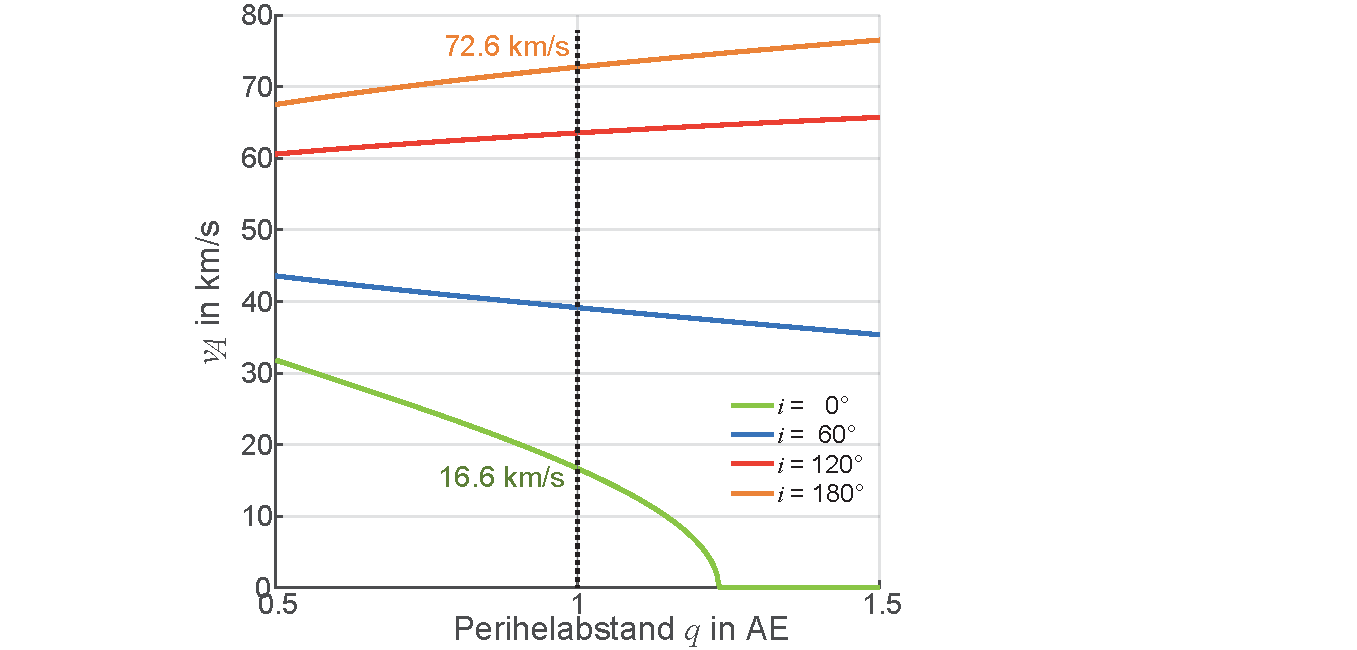
\includegraphics[width=\textwidth]{Aufschlaggeschwindigkeit.pdf}%
\caption[Aufschlaggeschwindigkeit eines Kometen.]{Berechnete Aufschlaggeschwindigkeit eines Kometen f�r verschiedene Bahnneigungen als Funktion des Perihelabstandes.}%
\label{abb:hm_aufschlaggeschw_2}%
\end{figure}

Wir k�nnen \eqref{eq:hm_hmlsg_24b_7} und \eqref{eq:hm_hmlsg_24b_9} auch benutzen, um die im Beispiel \ref{bsp:hm_shoemaker_levy} berechnete Aufschlaggeschwindigkeit des Kometen SL9 zu �berpr�fen.
Wir m�ssen in unseren Gleichungen nur folgende Ersetzungen vornehmen:
\begin{align*}
	a_\text{\earth} &\rightarrow a_\text{\jupiter} = 5.204\:\text{AE} \\
	R_\text{\earth} &\rightarrow R_\text{\jupiter} = 71492\:\text{km} \\
	\alpha &\rightarrow \alpha_\text{\jupiter} = \frac{m_\text{\jupiter}}{m_\text{\astrosun}} = 0.955\cdot 10^{-3} ~~.
\end{align*}
Mit diesen Werten und den Bahnparametern von SL9 aus Tabelle \ref{tab:hm_bahnparameter} erhalten wir $v_\text{A,SL}\!=\!59.5\:\text{km/s}$, was gut mit den numerisch berechneten Werten in Beispiel \ref{bsp:hm_shoemaker_levy} �bereinstimmt.\\

\item Aus \eqref{eq:hm_Shoemaker1979} erh�lt man f�r die kinetische Energien des Meteoriten im N�rdlinger Ries \bzw Steinheimer Becken
\begin{equation*}
T_\text{N} \approx 141\:\text{Gt TNT}  ~~ \text{bzw.} ~~ T_\text{S} \approx 268\:\text{Mt TNT} ~~.
\end{equation*}
Zum Vergleich, die Atombombe von Hiroshima hatte eine Sprengkraft von \anf{nur} ca. $12\:\text{kt TNT}$.
Die Energien von solchen Asteroiden/Meteoriten sind also unglaublich hoch (Man dr�cke diese einmal in konventionellen Gr��en ($1\:$kt TNT entspricht $4.185\cdot 10^{12}\:\text{J}$ aus.).\\
Unter Annahme eines kugelf�rmigen Himmelsk�rpers mit der Dichte $\rho\!=\!2.8\:\text{g/cm}^3$ kann man den Durchmesser des Meteoriten absch�tzen.
Im L�sungsteil (b) (\figref{hm_aufschlaggeschw_2}) hatten wir f�r $v_\text{min}$ und $v_\text{max}$ Werte zwischen 16 und 70 km/s erhalten.
Da es sehr wahrscheinlich ist, dass die Inklination der Asteroidenbahn zwischen $20\degree$ und $45\degree$ lag, k�nnen wir von Aufschlaggeschwindigkeiten zwischen $20$ km/s und $30$ km/s ausgehen.
Es ergeben sich dann Asteroidendurchmesser im Fall des N�rdlinger Ries von
\begin{equation*}
D_\text{N} = 2\,\sqrt[3]{\frac{T_\text{N}}{\pi\rho v_\text{A}^2}} = 1.0\:\text{km}~\ldots~ 1.3\:\text{km}
\end{equation*}
und im Fall des Steinheimer Beckens von
\begin{equation*}
D_\text{S} = = 0.5\:\text{km}~\ldots~ 0.65\:\text{km}~.
\end{equation*}

\begin{figure}[H]
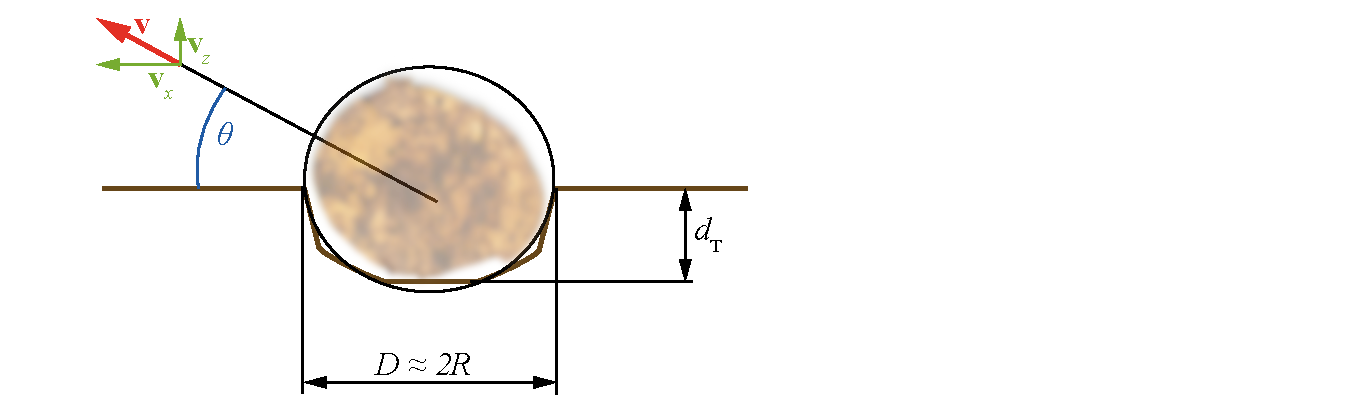
\includegraphics[width=\textwidth]{Meteorkrater.pdf}%
\caption{Zur Berechnung der Aufschlaggeschwindigkeit eines Kometen}%
\label{abb:hm_shoemaker_deriv}%
\end{figure}

Wir wollen jetzt noch eine Absch�tzung f�r die Shoemaker-Formel geben. Dazu nehmen wir an, dass die vom Asteroiden (oder einem anderen Himmelsk�rper) ausgeworfene Kratermasse unter einem Winkel von $\theta$ und mit einer Geschwindigkeit $v$ wegfliegt. Die Mindestzeit, die die ausgeworfene Masse in der Luft sein muss, ergibt sich nach \figref{hm_shoemaker_deriv}
zu:
	\[t = 2 v_z/g = 2v\sin\theta/g
\]
In dieser Zeit muss der Kraterdurchmesser $D=2 R$ "`ausgehoben"' werden, also:
	\[ D = v_x\,t = 2v^2\,\sin\theta \cos\theta/g = v^2 \,\sin(2\theta)/g \leq v^2/g\,
\]
woraus folgt : $v_\text{min} = \sqrt{D\,g}$.
Die Masse des Aushubs ist (Krater als zylinderf�rmig angenommen):
	\[ m_\text{A} = \varrho\frac{\pi}{4}\,D^2\,d_\text{T}\,,
	\]
	mit $\varrho \approx \SI{4e3}{\kg\per\metre\cubed}$.
Damit ist eine minimale kinetische Energie verbunden, die den Auswurf "`wegtransportiert"';
	\[ T_\text{min} = \frac{m_\text{A}}{2} \,v^2 = \frac{\pi}{8}\varrho\,g\,d_\text{T}\,D^3\,.
	\]
Ber�cksichtigt man noch, dass wegen der Umwandlung in thermische Energie nur wenige Prozent $\eta = 1\% \ldots 4\%$ in kinetische Energie umgewandelt werden, dann gilt die Beziehung:
\begin{align}
T_\text{min}  = \tilde{\kappa}\,	T_\text{K} = \tilde{\kappa} \frac{\pi}{8}\varrho\,g\,d_\text{T}\,d_\text{T}\,D^3\,. \,. \label{eq:hm_shoemaker_verified}
\end{align}
Wir bekommen also ann�hernd den empirischen Zusammenhang $D \propto T_\text{K}^{1/3}$, wobei wegen $\tilde{\kappa} = \tilde{\kappa}(d)=\tilde{\kappa}(d(D))$ eine zus�tzliche $D-$Abh�ngigkeit ergibt, die sich in der Shoemaker-Formel im Exponenten zeigt. Wir �berlassen es dem Leser, in Formel \eqref{eq:hm_shoemaker_verified} den Proportionalit�tsfaktor $\tilde{\kappa}$ auszurechnen und zu verifizieren, dass sich tats�chlich solche gigantischen Energien ergeben.\\

\item Nehmen wir an, dass der Planetoid (Meteor) mit Masse $m_\text{P}$ einen Mond der Masse $m_\text{M}$ hatte.
  Dann zieht der Planetoid den Mond mit der Kraft $F_\text{P}\!=\! Gm_\text{P}m_\text{M}/d^2$ an.
  Andererseits wirkt auf die beiden K�rper die Gravitationskraft der Sonne in unterschiedlichem Ma�e (Gezeitenkraft) (siehe \kap{hm_gezeiten}), die die beiden K�rper zu trennen versucht. F�r f�r die Gezeitenkraft gilt:
\begin{equation*}
F_\text{Gez} \approx \frac{2Gm_\text{M}m_\text{\astrosun}\,a_\text{PM}}{a_\text{\earth}^3}~~,
\end{equation*}  
worin $a_\text{PM}$ der Abstand zwischen Planetoid und Mond ist.
Das System des Doppelplanetoiden (bzw. Planetoid mit Mond) ist stabil, wenn $F_\text{P}\!>\!F_\text{Gez}$, also
\begin{equation*}
\frac{Gm_\text{P}m_\text{M}}{a_\text{PM}{}^2} > \frac{2Gm_\text{M}m_\text{\astrosun}\, a_\text{PM}}{a_\text{\earth}^3}~~.
\end{equation*}
Dies ist erf�llt, wenn
\begin{equation*}
	a_\text{PM} < \sqrt[3]{\frac{m_\text{P}}{2m_\text{\astrosun}} a_\text{\earth}^3} = a_\text{\earth}\,\sqrt[3]{\frac{m_\text{P}}{2m_\text{\astrosun}}} ~~.
\end{equation*}
Mit der Masse $m_\text{P}\!=\!\rho_\text{P}V_\text{P}$ aus Aufgabenteil (c) erhalten wir $a_\text{PM}\!\leq\! 150\:$km.
Verglichen mit dem Abstand der beiden Einschlagkrater von $40\:$km ist es also wahrscheinlich oder zumindest m�glich, dass der Doppelkrater vor 15 Millionen Jahren durch einen Doppelplanetoiden bzw. Planetoid und zugeh�riger Mond verursachte wurde.
\end{enumerate}
Die �bungsaufgabe und deren L�sung basiert auf der Darstellung �hnlicher Probleme in \cite{Garfinkle2014} und \cite{Quetz2017}.
Wir verweisen auch auf das entsprechende \mscr~\mlhmref{VerweildauerKomet.m} sowie \mlhmref{AufprallgeschwindigkeitKomet.m}.
\medskip \end{sol}

\textcolor{blue} {$\rightarrow$ zur} \probref{hm_verweildauer_komet_erdbahn}.\\
\noindent\rule[1ex]{\textwidth}{0.5pt} \newpage


%-----------------------------------------------------------------------------------------------------------

\begin{sol}{prob:hm_Doppelstern}\label{lsg:hm_Doppelstern} %�bung27
\textbf{Doppelstern-System - Vergleich numerische und analytische L�sung} \\ \\

Die Rechnungen finden sich f�r ein Modellsystem mit Massenverh�ltnis 2.5:1 und einem anf�nglichen Abstand von 2\,AE, sowie anf�nglichen Geschwindigkeiten in Oppositionsstellung von $v_0 = \SI{-5}{\km\per\second}$ \bzw $v_0 = \SI{20}{\km\per\second}$ in den \mscr en \mlhmref{Doppelsternsystem.m} (Inertialsystem) \bzw \mlhmref{DoppelsternsystemCOM.m} (Schwerpunktsystem). L�sungen sind beispielhaft in den folgenden Abbildungen gezeigt.\\
%Die numerische �bereinstimmung mit der analytischen L�sung ist ausgezeichnet.
\begin{figure}[H]
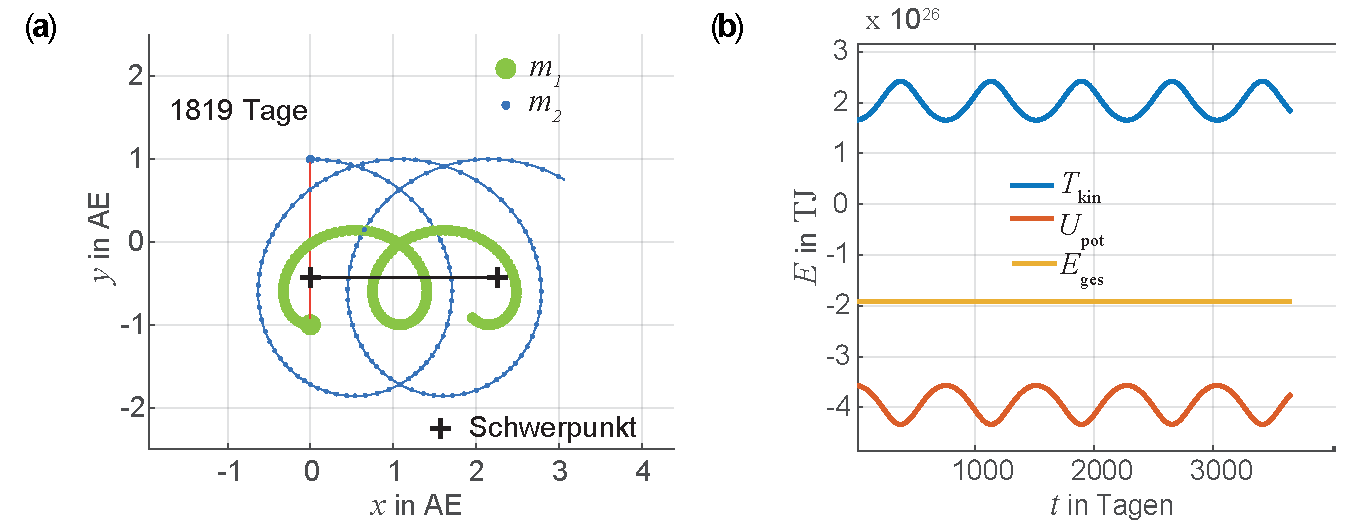
\includegraphics[width=\textwidth]{DoppelsternEnergie.pdf}%
\caption{Trajektorie \fa und Energieanteile \fb eines Doppelsternsystems im Inertialsystem. Die Energieerhaltung mit dem Hin-und Herpendeln zwischen kinetischer und potentieller Energie ist gut zu erkennen}%
\label{abb:hm_doppelsternenergie}%
\end{figure}
\begin{figure}[H]
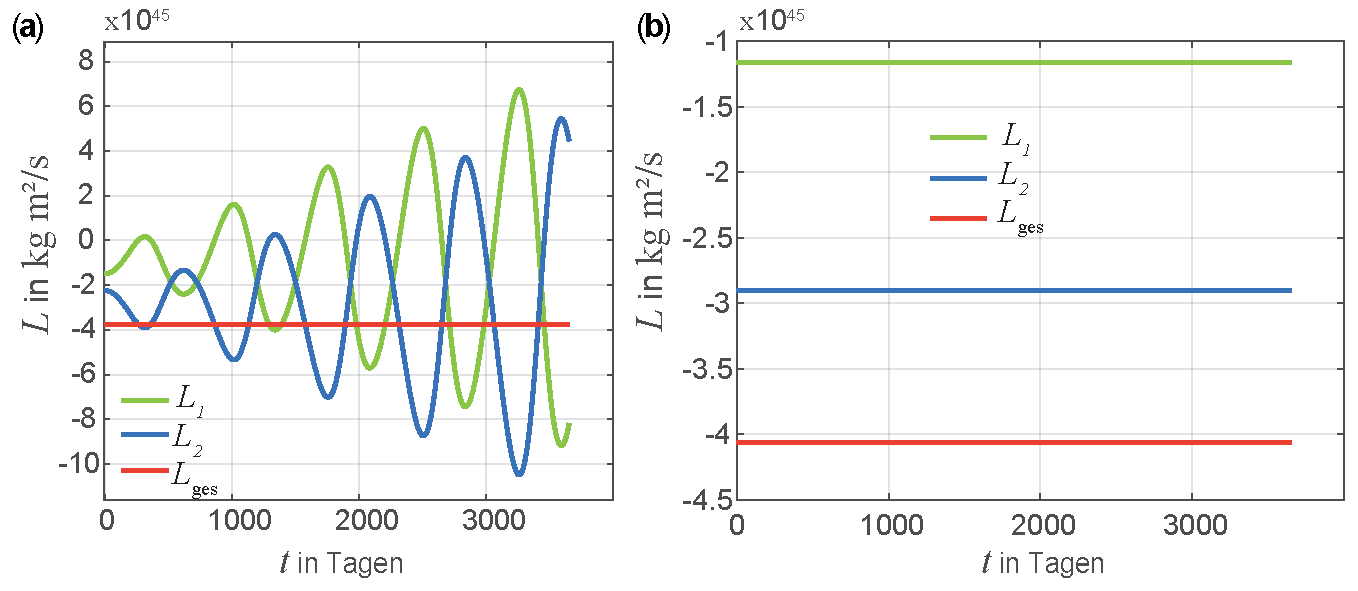
\includegraphics[width= \textwidth]{DoppelsternDrehimpulse.pdf}%
\caption{Drehimpulse eines Doppelsternsystems im Inertialsystem \fa und im Schwerpunktsystem \fb. Im Inertialsystem ist der Gesamtdrehimpuls erhalten}%
\label{abb:hm_doppelsterndrehimpulse}%
\end{figure}
\end{sol}
\textcolor{blue} {$\rightarrow$ zur} \probref{hm_Doppelstern}.\\
\noindent\rule[1ex]{\textwidth}{0.5pt} \newpage

%-----------------------------------------------------------------------------------------------------------

\begin{sol}{prob:hm_Sonnensystem}\label{lsg:hm_Sonnensystem} %�bung28
\textbf{Sonnensystem - Numerische, Kepler- und JPL-Berechnung} \\ \\

Wir verweisen auf die \mscr e \mlhmref{SonnensystemSimulationKepler.m}, \mlhmref{SonnensystemSimulationJPL.m} und \mlhmref{SonnensystemSimulationLangeZeiten.m}.\\
Als Referenzdaten verwenden wir die Vektordaten aus \url{https://ssd.jpl.nasa.gov/horizons/} (\cite{JPL2020}).

Die Bewegungsgleichungen f�r die Beschleunigungen der einzelnen ($i,j = 1 \ldots 8$) Planeten und die beiden betrachteten Kometen ($i,j = 9,10$) und die Sonne ($i,j = =N=11$) lauten dann:
	\begin{align}
		 \vec{a}_i = \ddot{\vec{r}}_i = -\sum_{j, j \neq i}^{N} (\vec{r}_i-\vec{r}_j) \frac{G\,m_i}{|\vec{r}_i-\vec{r}_j|^3}~~~~i=1 \ldots N~\,. \label{eq:hm_PlanetenDGLSystem01}
	\end{align}
Hierin sind $\vec{r}_i$ und $m_i$ die Positionsvektoren \bzw die Massen der einzelnen Planeten,  Kometen und der Sonne. Der Index $i,kj=N+1$ bezieht sich dabei auf die Sonne.
Die DGLs \eqref{eq:hm_PlanetenDGLSystem01} werden mit den entsprechenden Anfangsbedingungen f�r die Himmelsk�rper numerisch integriert. 

In \figref{hm_SonnensystemSimulation01} vergleichen wir die Abweichungen der L�sungen f�r \eqref{eq:hm_PlanetenDGLSystem01}, die wir aus der L�sung der Kepler-Gleichung \bzw der St�rungstheorie und zum anderen �ber numerische Integration von \eqref{eq:hm_PlanetenDGLSystem01} erhalten haben. Die Anfangswerte $\vec{r}_i(t_0)$ und $\dot{\vec{r}}_i(t_0)$  beschaffen wir uns aus dem JPL-Webservice \url{https://ssd.jpl.nasa.gov/horizons/}. Bei der Erdbahn erkennt eine periodische Abweichung (im Monatsrhythmus) unserer Rechnung von der JPL-Berechnung, die nat�rlich, davon herr�hrt, dass wir den Mond in unseren Rechnungen nicht ber�cksichtigt haben. Ansonsten ist die �bereinstimmung aber sehr gut und die Rechnung viel genauer als die einfache Kepler-L�sung, was man auch an der berechneten Marsbahn sehr gut sieht (bei der ja kein Mond der Gr��enordnung des Erdmondes zu ber�cksichtigen ist). Wir empfehlen dem interessierten Leser, die Rechnungen unter Ber�cksichtigung des Mondes zu wiederholen.

\begin{figure}[H]
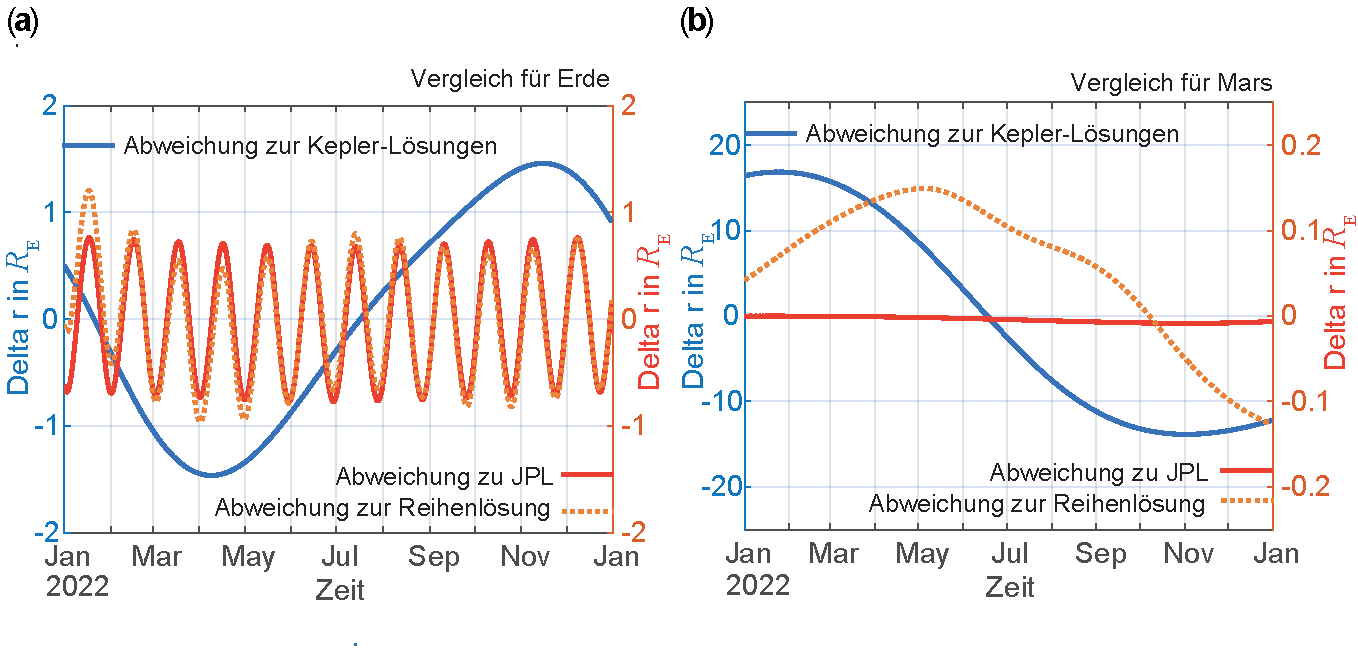
\includegraphics[width=\textwidth]{SonnensystemSimulation01.pdf}%
\caption[Sonnensystem-Simulation durch numerischen L�sung der Newtonschen Bewegungsgleichungen.]{Sonnensystem-Simulation durch numerischen L�sung der Newtonschen Bewegungsgleichungen. Abweichungen der L�sungen f�r die Bahn der Erde \fa und des Mars \fb von den Referenzdaten des JPL (\url{https://ssd.jpl.nasa.gov/horizons/}). Zum Vergleich sind auch die Abweichungen zur einfachen Kepler-L�sung und zur Reihenentwicklung nach der St�rungstheorie (\kap{Reihenentwicklung}) gezeigt.}%
\label{abb:hm_SonnensystemSimulation01}%
\end{figure}

In \figref{hm_SonnensystemSimulation02} zeigen wir die berechnete Bewegung des Schwerpunktes gegen�ber der Ausgangsposition. Eigentlich sollte dieser ja nach Definition in der Nulllage verbleiben. Die sehr kleine (man beachte die Achseneinteilung) systematische Drift resultiert aus der Tatsache, dass wir ja nicht �ber alle K�rper des Sonnensystems integriert haben. Es feheln ja etliche Monde, Kometen und Asteroiden. Die Gr��e der Drift ist f�r uns auch eine Aussage zur Genauigkeit der Integration.\\
%Es ist gar nicht so einfach die Frage zu beantworten, wie man f�r das Sonnensystem den Ursprung des Inertialsystems findet. Die IAU (\textit{International Astronomical Union}) hat �ber sehr pr�zise (\textit{Very Large Base Interferometry} - VLBI) Messungen
%von extra-galaktischen Quellen das sogenannte ICRF3-Koordinatensystem (International Celestial Reference Frame 3) definiert. Der Schwerpunkt dessen Sonnensystems (\textit{Solar System Bary Center}-SSBC) wird (nicht-relativistisch) definiert durch:
% 	\begin{align}
%		 \vec{R}_\text{SSBC}  = \lk \sum_j  m_i\vec{r}_i\rk \bigg/ \lk \sum_j m_j \rk \,, \label{eq:hm_PlanetenDGLSystem02}
%	\end{align}
%wobei �ber alle K�rper des Sonnensystems summiert wird.\\
%Der Leser wird m�glicherweise auch die Frage stellen, wie die hochgenauen Daten des JPL zustande kommen. Keine Frage, die Ephemeriden des JPL sind sehr gut, aber sie sind sicherlich nicht auf den Bruchteil eines Millimeters genau, obwohl sie mit so vielen Dezimalstellen angegeben werden. Zur Erstellung einer JPL Ephemeride weren mehrere Beobachtungsdaten (optische, Radardaten und Raumfahrzeug-Daten) mit dynamischen Modellen kombiniert, insofern ist die JPL Ephemeride eine "`gemischt beobachtete-gerechnete"' Ephemeride und hat sowohl als Messwert als auch Modellergebnis Ungenauigkeiten. Es wird eine optimale Anpassung entwickelt, um diese Fehler statistisch zu minimieren. Die resultierende Ephemeride ist mit einer stark reduzierten Unsicherheit verbunden. Obwohl die Vektordaten des JPL mit 16 Dezimalstellen ausgegeben werden, bedeutet das nicht, dass alle Ziffern physikalisch sinnvoll sind. Die gesamte Zahl der Stellen wird bei unseren Rechen- und Modellgenauigkeiten nat�rlich nicht ben�tigt. 

\begin{figure}[H]
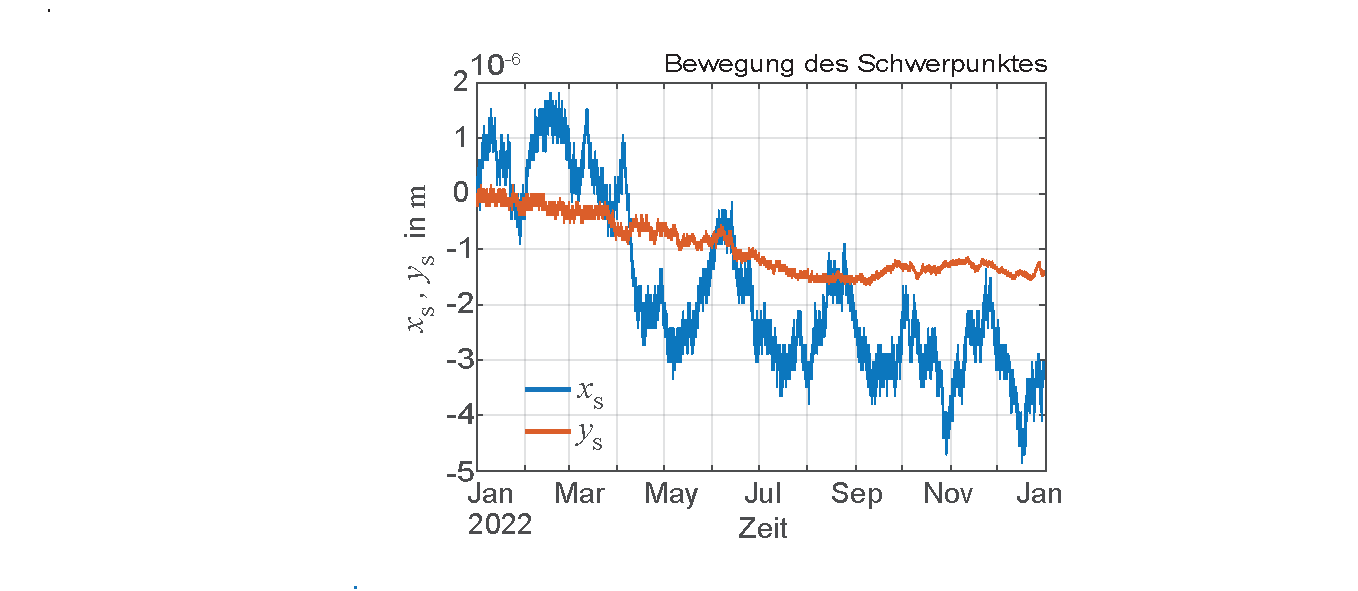
\includegraphics[width=\textwidth]{SonnensystemSimulation02.pdf}%
\caption[Sonnensystem-Simulation durch numerischen L�sung der Newtonschen Bewegungsgleichungen. Bewegung des Schwerpunktes.]{Sonnensystem-Simulation durch numerischen L�sung der Newtonschen Bewegungsgleichungen. Bewegung des Schwerpunktes.}%
\label{abb:hm_SonnensystemSimulation02}%
\end{figure}

In \figref{hm_SonnensystemSimulation03} vergleichen wir die numerischen L�sungen f�r \eqref{eq:hm_PlanetenDGLSystem01} f�r einen Zeitraum von 110 Jahren und \figref{hm_SonnensystemSimulation04} zeigt die Bewegung der Sonne aus der numerischen Integration von  \eqref{eq:hm_PlanetenDGLSystem01} relativ zum Baryzentrum des Sonnensystems (\mscr{}~ \mlhmref{SonnensystemSimulationLangeZeiten.m}) f�r den gleichen Zeitraum.

\begin{figure}[H]
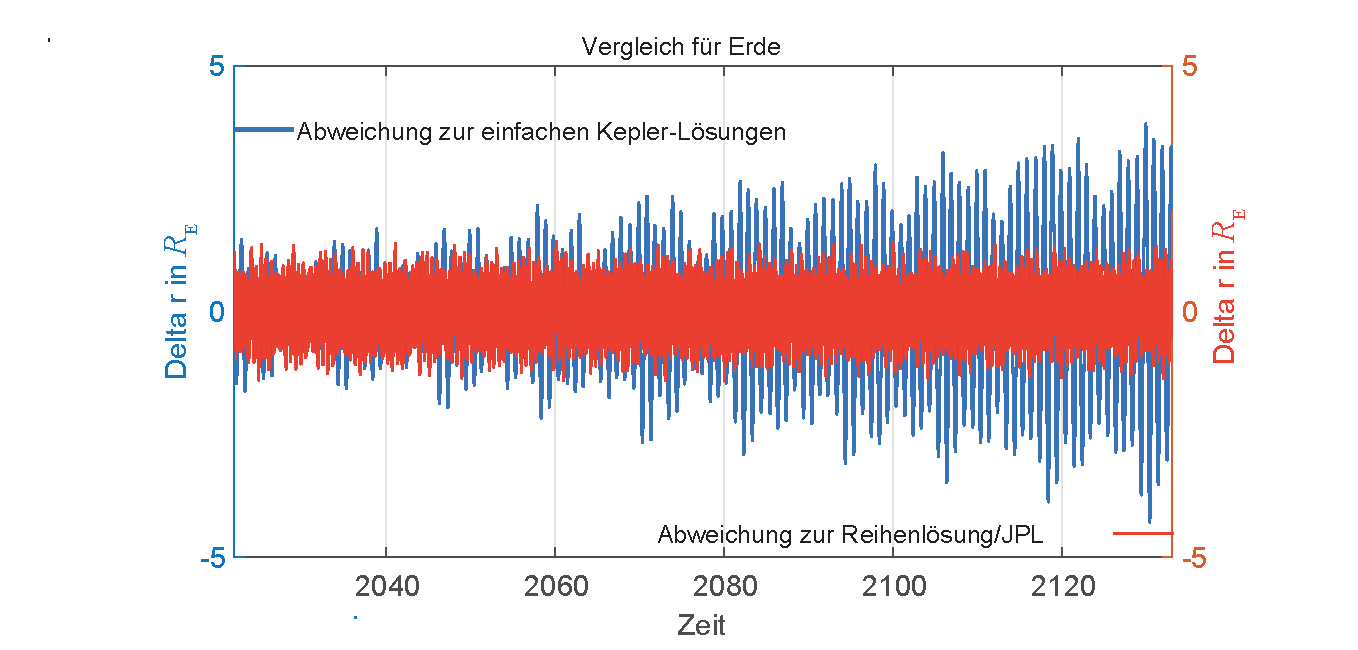
\includegraphics[width=\textwidth]{SonnensystemSimulation03.pdf}%
\caption[Sonnensystem-Simulation durch numerischen L�sung der Newtonschen Bewegungsgleichungen �ber lange Zeiten.]{Sonnensystem-Simulation durch numerischen L�sung der Newtonschen Bewegungsgleichungen �ber lange Zeiten. Abweichungen der L�sungen f�r die Bahn der Erde von den Referenzdaten des JPL (\url{https://ssd.jpl.nasa.gov/horizons/}). Zum Vergleich sind auch die Abweichungen der einfachen Kepler-L�sung zu den JPL Daten gezeigt.}%
\label{abb:hm_SonnensystemSimulation03}%
\end{figure}

\begin{figure}[H]
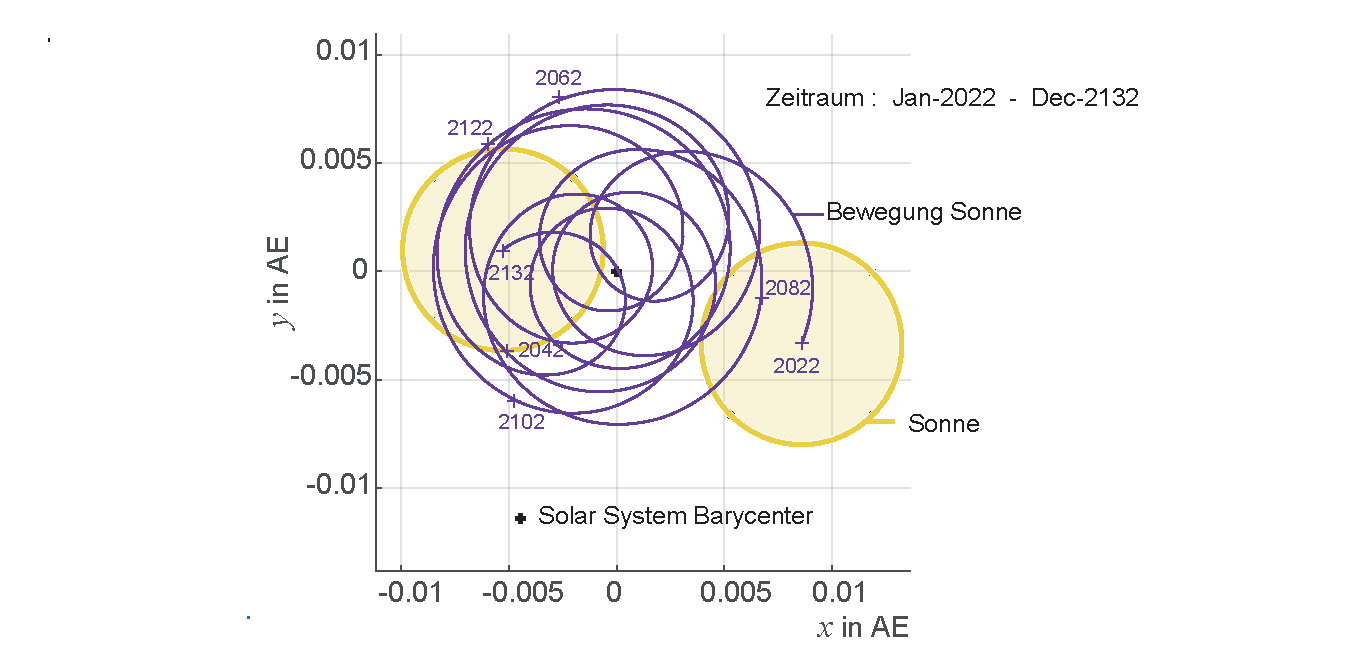
\includegraphics[width=\textwidth]{SonnensystemSimulation04.pdf}%
\caption[Sonnensystem-Simulation durch numerischen L�sung der Newtonschen Bewegungsgleichungen. Bewegung der Sonne im ICRF �ber 120 Jahre.]{Sonnensystem-Simulation durch numerischen L�sung der Newtonschen Bewegungsgleichungen. Bewegung der Sonne im ICRF �ber 110 Jahre. Die Anfangswerte $\vec{r}_i(t_0)$ und $\dot{\vec{r}}_i(t_0)$ haben wir uns wieder aus dem JPL-Webservice beschafft. Vergleiche dazu auch die Ergebnisse in \cite{Park2021}}%
\label{abb:hm_SonnensystemSimulation04}%
\end{figure}

Es ist gar nicht so einfach die Frage zu beantworten, wie man f�r das Sonnensystem den Ursprung des Inertialsystems findet. Die IAU ((\textit{International Astronomical Union})) hat �ber sehr pr�zise (\textit{Very Large Base Interferometry} - VLBI) Messungen
von extra-galaktischen Quellen das sogenannte ICRF3-Koordinatensystem (International Celestial Reference Frame 3) definiert. Der Schwerpunkt dessen Sonnensystems (\textit{Solar System Bary Center}-SSBC) wird (nicht-relativistisch) definiert durch:
 	\begin{align}
		 \vec{R}_\text{SSBC}  = \lk \sum_j  m_i\vec{r}_i\rk \bigg/ \lk \sum_j m_j \rk \,, \label{eq:hm_PlanetenDGLSystem03}
	\end{align}
wobei �ber alle K�rper des Sonnensystems summiert wird.\\
Der Leser wird m�glicherweise auch die Frage stellen, wie die hochgenauen Daten des JPL zustande kommen. Keine Frage, die Ephemeriden des JPL sind sehr gut, aber sie sind sicherlich nicht auf den Bruchteil eines Millimeters genau, obwohl sie mit so vielen Dezimalstellen angegeben werden. Zur Erstellung einer JPL Ephemeride weren mehrere Beobachtungsdaten (optische, Radardaten und Raumfahrzeug-Daten) mit dynamischen Modellen kombiniert, insofern ist die JPL Ephemeride eine "`gemischt beobachtete-gerechnete"' Ephemeride und hat sowohl als Messwert als auch Modellergebnis Ungenauigkeiten. Es wird eine optimale Anpassung entwickelt, um diese Fehler statistisch zu minimieren. Die resultierende Ephemeride ist mit einer stark reduzierten Unsicherheit verbunden. Obwohl die Vektordaten des JPL mit 16 Dezimalstellen ausgegeben werden, bedeutet das nicht, dass alle Ziffern physikalisch sinnvoll sind. Die gesamte Zahl der Stellen wird bei unseren Rechen- und Modellgenauigkeiten nat�rlich nicht ben�tigt. 
Sehr lesenswert zu diesem Thema ist f�r interessierte Leser die Referenz \cite{Park2021}.

\medskip \end{sol}

\textcolor{blue} {$\rightarrow$ zur} \probref{hm_Sonnensystem}.\\
\noindent\rule[1ex]{\textwidth}{0.5pt} \newpage

%-----------------------------------------------------------------------------------------------------------

\begin{sol}{prob:hm_Dreifachstern}\label{lsg:hm_Dreifachstern} %�bung29
\textbf{Dreik�rper-System - L�sung f�r 3 identische Massen} 
\begin{itemize}
	\item \textit{\textbf{Anordnung 1 - Achtf�rmige Trajektorien}}\\

Die Rechnungen sind im \mscr{}~ \mlhmref{DreiKoerperProblem01.m} hinterlegt.
\begin{figure}[H]
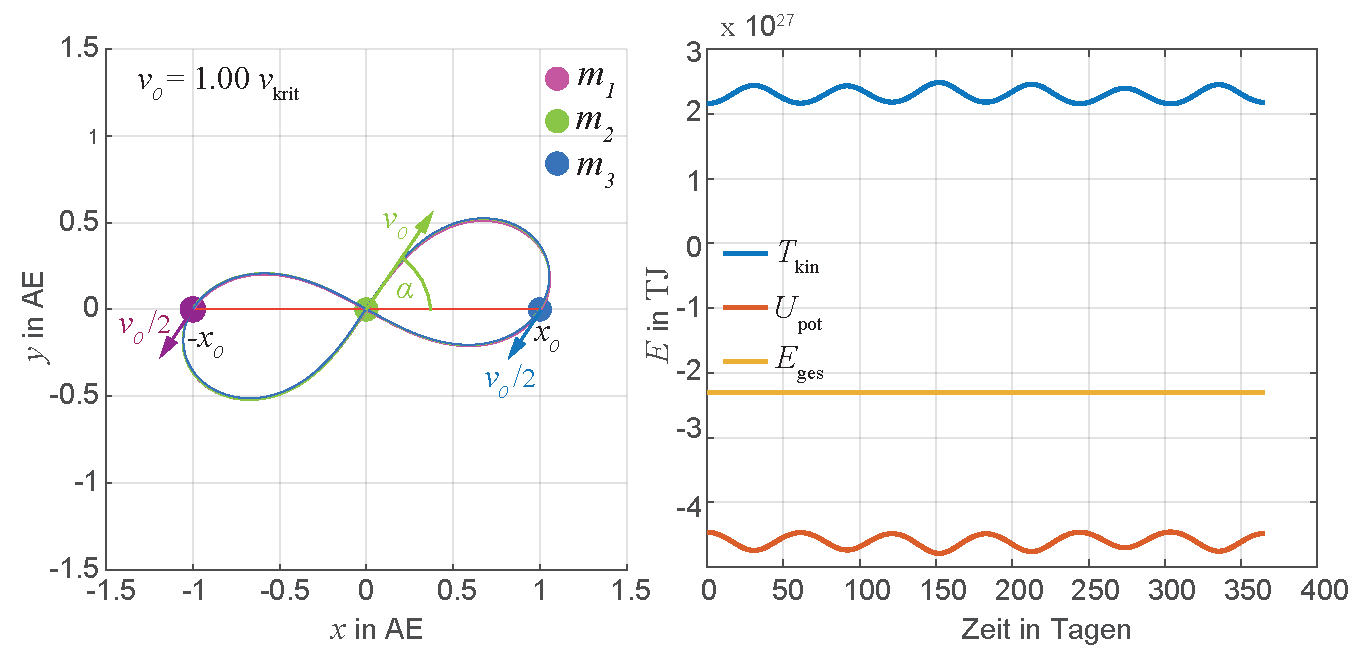
\includegraphics[width=0.9\textwidth]{DreiKoerperSystem01.pdf}%
\caption[Dreik�rperproblem mit Bewegung in Form einer Acht.]{Dreik�rperproblem mit Bewegung in Form einer Acht. Die Geschwindigkeit $v_0=v(t_0)$ ist genau der kritischen Geschwindigkeit $v_\text{krit} = 1.27\,\sqrt{G \, m / x_0}$, worin $2\,x(t_0)$ der Anfangsabstand der beiden �u�eren Massen $m_1$ und $m_3$ auf der $x$-Achse ist. Der Winkel von $\vec{v}_0$ zur $x$-Achse betr�gt $56.9\degree$ \cite{Moore1993, Chenciner2000}. Man erh�lt in diesem Fall stabile Bahnen.}
\label{abb:hm_DreiKoerperSystem01}%
\end{figure}
\begin{figure}[H]
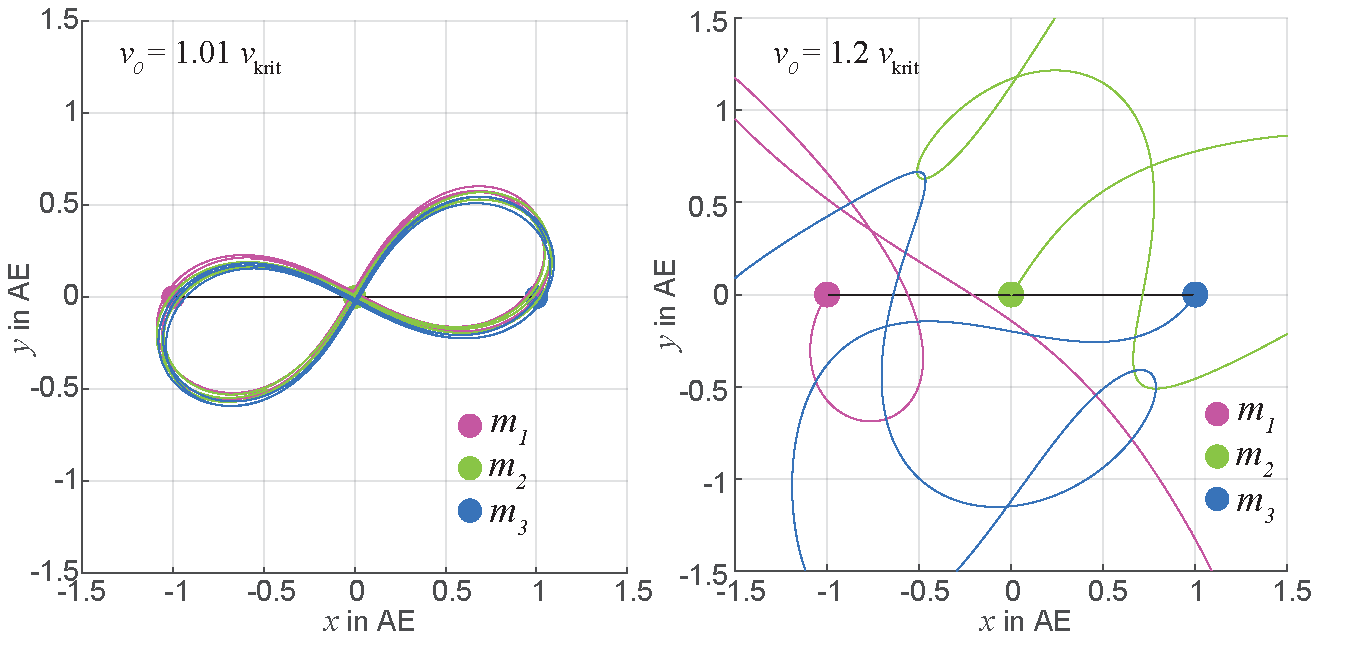
\includegraphics[width=0.9\textwidth]{DreiKoerperSystem02.pdf}%
\caption[Dreik�rperproblem mit Bewegung in Form einer Acht.]{Dreik�rperproblem mit Bewegung in Form einer Acht. Die Geschwindigkeit $v_0$ weicht 1\% (linkes Bild) \bzw 20\% von der der kritischen Geschwindigkeit $v_\text{krit} = 1.27\,\sqrt{(G \, m_0 / x_0)}$ ab. Man erkennt, dass man im linken Bild noch quasistabile Bahnen bekommt, im Fall rechts geht das System sehr schnell in einen chaotischen Zustand �ber.}
\label{abb:hm_DreiKoerperSystem02}%
\end{figure}
	
\newpage
	\item \textit{\textbf{Anordnung 2 - Gleichseitiges Dreieck}}\\
	
Wir k�nnen f�r diesen Fall auf Grund der Symmetrie leicht ableiten, dass die resultierende Kraft aus der Gravitation von den zwei anderen Massen auf die betrachtete betrachtete Masse (in \figref{hm_DreiKoerperSystemDreieck} $m_1$) jeweils in Richtung gemeinsamer Schwerpunkt zeigt und damit als Radialkraft die Massen auf eine kreisf�rmige Umlaufbahn zwingt. (Der Radius der Bahn ist dann gerade der Radius des Umkreises des gleichseitigen Dreiecks.)

\begin{figure}[H]
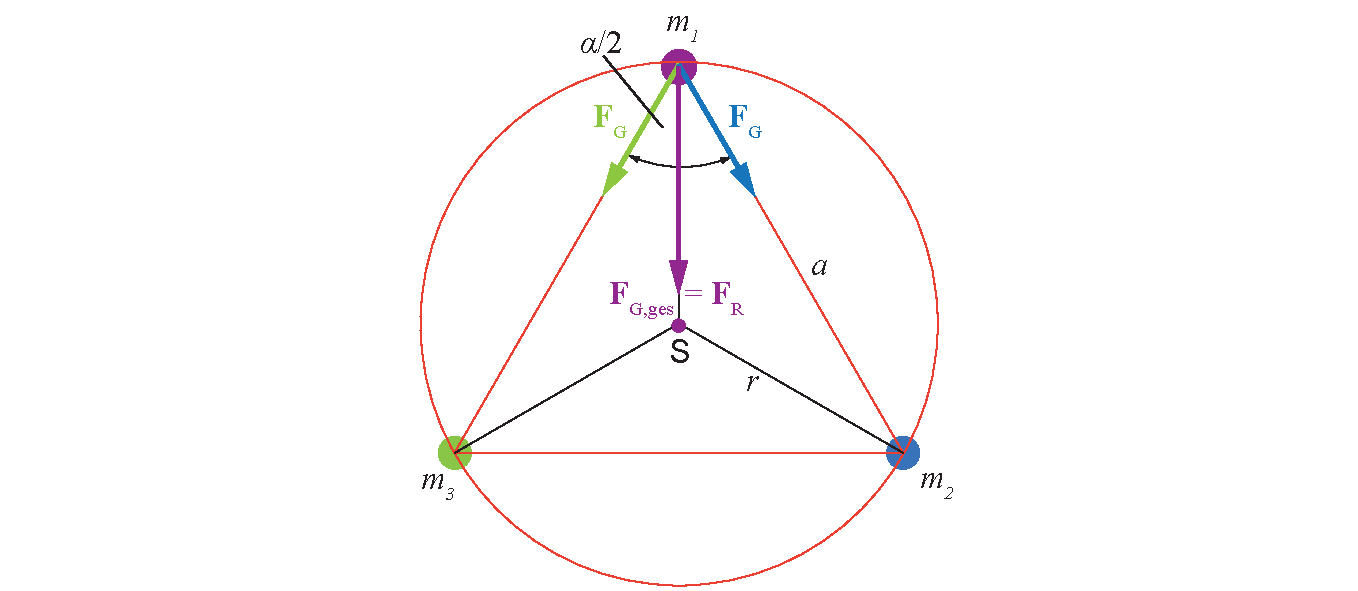
\includegraphics[width=0.9\textwidth]{DreiKoerperSystemDreieck.pdf}%
\caption[Geometrie des Dreik�rperproblem in Form eines gleichseitigen Dreiecks mit Drehung um Schwerpunkt. ]{Geometrie des Dreik�rperproblems in Form eines gleichseitigen Dreiecks mit Drehung um Schwerpunkt.}
\label{abb:hm_DreiKoerperSystemDreieck}%
\end{figure}

Wir wollen die Umlaufgeschwindigkeit berechnen. Dazu berechnen wir mit der Geometrie von \figref{hm_DreiKoerperSystemDreieck} die Gesamtkraft der Massen $m_2=m$ und $m_3=m$ auf die Masse $m_1=m$ zu:
\begin{align}
	\vec{F}_\text{G,ges} &=\frac{G m_1 m_2}{a^2}\,\begin{pmatrix} -\sin(\alpha/2) \\ \cos(\alpha/2 )\\ \end{pmatrix} + 
	        \frac{G m_1 m_3}{a^2}\,\begin{pmatrix} \sin(\alpha/2) \\ \cos(\alpha/2 )\\ \end{pmatrix} \nonumber \\
					&= 2\,\frac{G m^2}{a^2}\,\cos(\alpha/2)\, \veceY~~~~~\text{und mit}~\cos(\alpha/2)=\sqrt{3}/2~\text{, sowie}~d=r\,\sqrt{3} \,\nonumber \\
					&=\frac{G m^2}{\sqrt{3}\,r^2}\,\veceY\,.
	\label{eq:hm_DreiKoerperSystem01}				
\end{align}
Diese muss gleich der Radialkraft der Kreisbewegung sein, \dh:
\begin{align}
	\vec{F}_\text{R} &= \frac{m\,v^2}{r}\,\veceY = \frac{G m^2}{\sqrt{3}\,r^2}\,\veceY\,. 
	\label{eq:hm_DreiKoerperSystem02}				
\end{align}
Damit ergibt sich die Beziehung f�r die Geschwindigkeit: 
\begin{align}
	v = \sqrt{\frac{G\,m}{r\sqrt{3}}} = \sqrt{\frac{G\,m}{a}}\,.
	\label{eq:hm_DreiKoerperSystem03}				
\end{align}

F�r die Simulation im \mscr{}~ \mlhmref{DreiKoerperProblem02.m}\, nehmen wir einen Radius von einer Astronomischen Einheit und eine Masse der K�rper von zwei Sonnenmassen an. Wir erwarten daher eine Bewegung, die sich in der Zeitskala von Jahren abspielt. Das Programm simuliert 10-15 Jahre in Zeitschritten von einem Tag.
	
\begin{figure}[H]
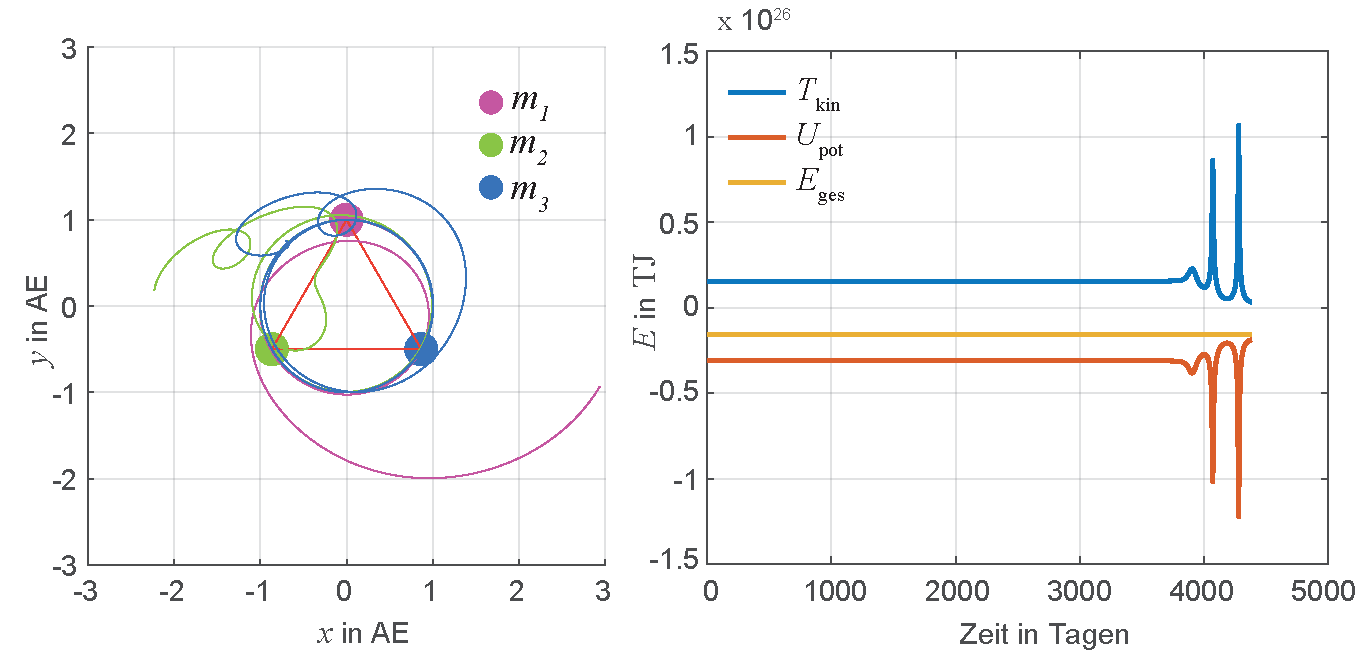
\includegraphics[width=0.9\textwidth]{DreiKoerperSystem03.pdf}%
\caption[Dreik�rperproblem in Form eines gleichseitigen Dreick mit Drehung um Schwerpunkt. ]{Dreik�rperproblem in Form eines gleichseitigen Dreiecks mit Drehung um Schwerpunkt. Man erkennt, dass das System nach einer anf�nglich stabilen Bahn in in einen chaotischen Zustand �bergeht. Dieser �bergangszeitpunkt (in unserem Fall in etwa bei \ca 10 Jahren) h�ngt stark von den Ungenauigkeiten der numerischen Rechnung ab. Man variiere dazu die Toleranzparameter in der options-Funktion des \odevf-Solvers.}
\label{abb:hm_DreiKoerperSystem03}%
\end{figure}
\end{itemize}

\medskip \end{sol}

\textcolor{blue} {$\rightarrow$ zur} \probref{hm_Dreifachstern}.\\
\noindent\rule[1ex]{\textwidth}{0.5pt} \newpage

%-----------------------------------------------------------------------------------------------------------

\begin{sol}{prob:hm_Tempel1_SwiftTuttle}\label{lsg:hm_Tempel1_SwiftTuttle} %�bung30
\textbf{Kometen im Sonnensystem -- Kollision mit der Erde?} \\ \\


Wir verweisen auf die \mscr e \mlhmref{KometenKollisionKepler.m}, \mlhmref{KometenKollisionSim.m} und \mlhmref{KometenKollisionJPL.m}.\\
Als Referenzdaten verwenden wir die Vektordaten aus \url{https://ssd.jpl.nasa.gov/horizons/} (\cite{JPL2020}).\\
Die Berechnung f�r die n�chste Ann�herung des Planeten im Jahr 2126 erfolgt �ber die Kepler-L�sung (\mlhmref{KometenKollisionKepler.m}), die numerische Integration der Bewegungsgleichungen mit den in \probref{hm_Sonnensystem} entwickelten Programmen und zum Vergleich �ber die JPL-Daten \mlhmref{KometenKollisionJPL.m}. Der Vergleich ergibt:
\begin{itemize}
	\item \textit{\textbf{Berechnung f�r 2126 �ber L�sung der Kepler-Gleichung}}\\
	
 Abstand Erdn�he :   0.91426408\,AE\,\,~ \bzw ~~ 1.3677e+08\,km\\
 Datum Erdn�he~~ :   24-Jun-2126\\

 Abstand Perihel :   0.95951616\,AE\,~~ \bzw ~~ 1.4354e+08\,km\\
 Datum Perihel~~ :   30-Apr-2126\\

\item \textit{\textbf{Berechnung f�r 2126 �ber numerische Integration der Bewegungsgleichungen \eqref{eq:hm_PlanetenDGLSystem01}}}\\ 

 Abstand Erdn�he :   0.15346854\,AE\,~~ \bzw ~~ 2.2959e+07\,km\\
 Datum Erdn�he~~ :   06-Aug-2126\\

 Abstand Perihel :   0.95630432\,AE\,~~ \bzw ~~ 1.4306e+08\,km\\
 Datum Perihel~~ :   12-Jul-2126\\

\item \textit{\textbf{Berechnungen des JPL}}\\ 

 Abstand Erdn�he :   0.1530400\,AE\,~~ \bzw ~~ 2.2894e+07\,km\\
 Datum Erdn�he~~ :   06-Aug-2126\\

 Abstand Perihel :   0.95416973\,AE\,~~ \bzw ~~ 1.4274e+08\,km\\
 Datum Perihel~~ :   14-Jul-2126\\

\end{itemize}

Die Ergebnisse der numerischen Integration der Bewegungsgleichungen �ber die Himmelsk�rper stimmen gut mit den JPL Daten �berein. Die einfache Kepler-Rechnung reicht offensichtlich nicht aus, der Komet wird auf seiner weiten Bahn offensichtlich von mehreren Himmelsk�rpern (insbesondere vom Jupiter) beeinflusst, so dass die einfache Zweik�rper-L�sung nicht mehr anwendbar ist. Nach unseren Rechnungen wird der Komet der Erde im Jahr 2026 zwar deutlich n�her kommen als in 1992, diese aber dennoch in einem Abstand von ca 20 Mio km passieren. Es droht also keine Kollisionsgefahr. Wir empfehlen aber dennoch Anfang 2125 mit neuen JPL Daten noch einmal nachzurechnen. In jedem Fall sollte der Komet sehr gut sichtbar werden.

Die Trajektorien von Swift-Tuttle sind f�r den Zeitraum von 110 Jahren \bzw in der Umgebung des Periheldurchgangs im Jahr 2126 in \figref{hm_SwiftTuttle01} dargestellt. \figref{hm_SwiftTuttle02} zeigt berechneten Trajektorien in der Umgebung des Periheldurchgangs im Jahr 2126 f�r die numerische Kepler-L�sung \bzw die  vollst�ndige Integration der Bewegungsgleichungen \eqref{eq:hm_PlanetenDGLSystem01} �ber "`alle"' Himmelsk�rper.

\begin{figure}[H]
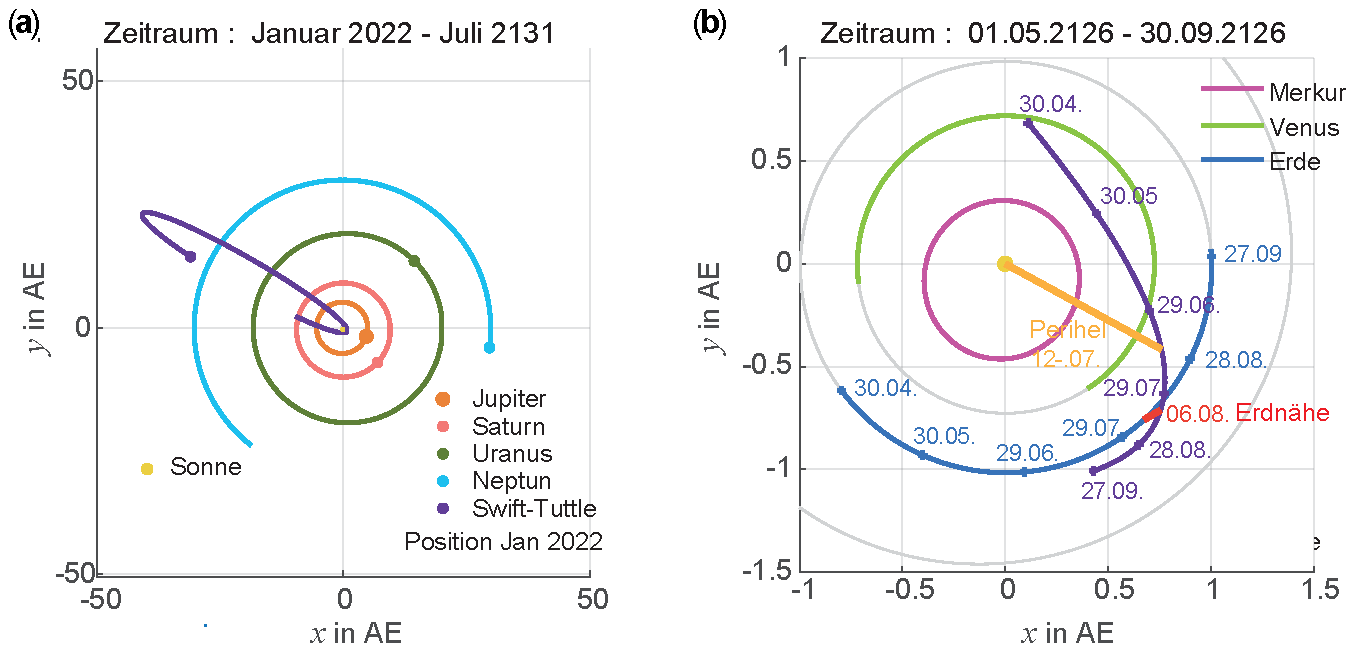
\includegraphics[width=\textwidth]{KometenKollision01.pdf}%
\caption[Trajektorien des Kometen Swift-Tuttle. ]{Berechnete Trajektorien des Kometen Swift-Tuttle. \fa Zeitraum 2022--2132  \fb Umgebung des Perihelduchgangs in 2126. Die Berechnung erfolgte durch numerische Integration der Bewegungsgleichungen \eqref{eq:hm_PlanetenDGLSystem01}.}
\label{abb:hm_SwiftTuttle01}%
\end{figure}

\begin{figure}[H]
\includegraphics[width=\textwidth]{KometenKollision02.pdf}%
\caption[Trajektorien des Kometen Swift-Tuttle zum Zeitpunkt Periheldurchgang in 2126.]{Berechnete Trajektorien des Kometen Swift-Tuttle zum Zeitpunkt des Periheldurchgangs in 2126. \fa Numerische Kepler-L�sung f�r den Kometen. \fb Numerische Integration der Bewegungsgleichungen \eqref{eq:hm_PlanetenDGLSystem01} �ber alle gr��eren Himmelsk�rper.}
\label{abb:hm_SwiftTuttle02}%
\end{figure}


\medskip \end{sol}

\textcolor{blue} {$\rightarrow$ zur} \probref{hm_Tempel1_SwiftTuttle}.\\
\noindent\rule[1ex]{\textwidth}{0.5pt} \newpage

%-----------------------------------------------------------------------------------------------------------

\begin{sol}{prob:hm_lichtlaufzeit}\label{lsg:hm_lichtlaufzeit} %�bung31
\textbf{Lichtlaufzeit, Unterschied $\ET-\UT$} \\ \\
Wir k�nnten zur L�sung der Aufgaben die verschiedenen \mscre zu den Kometen- und Asteroidenbahnen (\mlhmref{Kometenbahnen.m} und folgende) benutzen.
Wir wollen hier aber eine Absch�tzung machen und k�nnen uns daher das Leben etwas einfacher machen.
Wir nehmen an, dass Perihel und Perig�um in der ekliptikalen L�nge zusammenfallen und das beide in der Ekliptik liegen, \dh die ekliptikale Breite 0 ist.
Dies bedeutet, dass die Geschwindigkeit $v_\text{K}$ des Kometen maximal ist und ihre Richtung senkrecht zur Beobachtungsrichtung liegt.
Die Geschwindigkeit $v_\text{K}$ erh�lt man dann aus der vis-viva-Gleichung \eqref{eq:hm_vis-viva_polar} zu
	\[v_\text{K}^2=\mu_\text{G}\lk \frac{2}{q_\text{K}}-\frac{1}{a_\text{K}} \rk~,
\]
worin $q_\text{K}$ und $a_\text{K}$ der Perihelabstand bzw. die gro�e Halbachse der Kometenbahn sind.
Da f�r Kometen i.A. $a_\text{K}\gg q_\text{K}$ ist, gilt n�herungsweise
	\[v_\text{K} \approx \sqrt{\frac{2\mu_\text{G}}{q_\text{K}}} ~.
\]
Der Unterschied in astrometrischer und scheinbarer ekliptikaler L�nge ist dann gegeben durch:
	\[\Delta \lambda \approx \frac{v_\text{K} \Delta t}{q_\text{K}} = \frac{v_\text{K} (q_\text{K} /c)}{q_\text{K}} = \frac{1}{c} \sqrt{\frac{2\mu_\text{G}}{q_\text{K}}}.
\]
Unter der Annahme verschwindender ekliptikaler Breiten (siehe oben) und kleiner Zeiten $\Delta t$ k�nnen wir die Rektaszensions�nderung 
$\Delta \alpha$  aus der L�ngen�nderung  wie folgt 
	\[	\Delta \alpha = \Delta \lambda \cos \epsilon 
	\]
	berechnen, worin $\epsilon$ die Ekliptikschiefe ist.
        Wir erhalten dann f�r den Versatz auf der CCD in der Zwischenbildebene 
	\[\Delta x = \pm f \Delta \alpha ~~.
	\]
Das Bild des Kometen wird also dann im Bildfeld sein, wenn $\left| \Delta x \right| \leq 18 $ mm ist, wenn also gilt:
	\[\Delta x = \frac{f}{c} \sqrt{\frac{2\mu_\text{G}}{q_\text{K}}} \cos \epsilon \leq 18 \text{mm} 
	\]
Wir setzen f�r den Halleyschen Kometen (H) $q_\text{K} = 0.58 \text{AE}$ und f�r Neowise (N) $q_\text{K} = 0.29 \text{AE}$ ein und erhalten:
\begin{align*}
\Delta \alpha_\text{H} &= 0.58' ~~\text{ und } \Delta \alpha_\text{N} = 0.87'\\
v_\text{H}&= 55.3 \:\text{km/s} ~~\text{ und } ~v_\text{N} = 82.6\:\text{km/s}~\\
\Delta x_\text{H} &= 0.43\:\text{mm} ~~\text{ und } ~\Delta x_\text{N} = 0.63\:\text{mm}~,
\end{align*}
was merklich ist (30 Bogensekunden), aber noch deutlich innerhalb des Bildfeldes.
Folglich w�rde auch bei Benutzung von UT anstelle ET, was einer Lichtlaufzeit von ca. 1 min entspricht, ebenfalls ein messbarer Positionsfehler von ca. 6 bis 8 Bogensekunden entstehen, aber der Komet ebenfalls gut im Bildfeld sein.
F�r genaue Astronomie reicht die Nichtber�cksichtigung von $\Delta T$ nat�rlich nicht aus.
Wir berechnen jetzt die Zeit $\Delta t_\text{G}$ in der der Komet aus dem Bildfeld des mitgef�hrten Teleskops herauswandert.
Es gilt:
\[\Delta \alpha_\text{G} = \frac{18\:\text{mm}}{f} = \frac{v_\text{K} \Delta t_\text{G}}{\left| q_\text{K}-a_\text{earth}\right|} ~
\]
woraus f�r die beiden Zeiten 148 min bzw. 175 min folgt.
Das hei�t, dass selbst bei perfekt mitgef�hrtem Teleskop die Kometen nach zwei bis drei Stunden aus dem Teleskopbildfeld "`herauswandern"'.
Man kann also die Eigenbewegung der Kometen in einer Nacht sehr gut beobachten.
Die Rechnungen k�nnen nat�rlich auch im Detail mit dem \mscr~\mlhmref{Kometenbahnen.m} nachvollzogen werden. \\
\medskip \end{sol}
\textcolor{blue} {$\rightarrow$ zur} \probref{hm_lichtlaufzeit}.\\
\noindent\rule[1ex]{\textwidth}{0.5pt} \newpage

%-----------------------------------------------------------------------------------------------------------
\newpage
%%%-----------------------------------------------------------------------------------------------------------
\subsection{�bungen zu Gezeiten}

%-----------------------------------------------------------------------------------------------------------

\begin{sol} {prob:hm_rochelimit} \label{lsg:hm_rochelimit} %�bung32
\textbf{Zur Herleitung des Roche-Limits.}\\ \\

Wir benutzen Abb. 1.14 (Band I), wobei im Bild Sonne/Mond durch Jupiter ersetzt werden muss und die Erde durch den Kometen.
Ebenso ersetzen wir $m \rightarrow m_\text{K},\,r \rightarrow d,\, R_\text{E} \rightarrow R_\text{K}.$
Wir betrachten den Punkt ($x=0$, $y=0$, $z=-R_\text{K}$). Dann wird aus Gleichung (1.103) aus Band I:\footnote{Alternativ kann man nat�rlich auch direkt Gleichung (1.103) aus Band I mit $\theta = 0$ \bzw $\theta = \pi$ benutzen.} 

\begin{align}
    \vec{g}_z = -\frac{2G\,m_\text{J}}{d^3}\,R_\text{K}\,\vec{e}_z \,. \label{eq:hm_lsgroche02}
\end{align}
\begin{align}
    g_z = -g_\text{Gez,V} &= g_0\,\frac{R_\text{E}}{r}\lk 3\cos^2\theta-1\rk = \frac{3}{2}\,g_0\,\frac{R_\text{E}}{r}\lk \cos2\theta+\frac{1}{3}\rk \,. 
\end{align}

Andersereits wirkt an dem Punkt die (Selbst-) Gravitation des Kometen:
\begin{align}
    g_\text{K} = + \frac{G\,m_\text{K}}{R_\text{K}{}^2}\,\vec{e}_z \,. \label{eq:hm_lsgroche03}
\end{align}
von \eqref{eq:hm_lsgroche02} und \eqref{eq:hm_lsgroche03} ergibt die effektiv wirkende Gravitationsbeschleunigung $g_\text{eff}$ auf den Kometen:
\begin{align}
    g_\text{eff} = \frac{G\,m_\text{K}}{R_\text{K}{}^2}\,\lk 1-2\,\frac{m_\text{J}}{m_\text{K}}\,\frac{R_\text{K}{}^3}{d^3}\rk \,, \label{eq:hm_lsgroche04}
\end{align}
welche f�r
\begin{align}
    d = r_\text{R} = \sqrt[3]{2\,\frac{m_\text{J}}{m_\text{K}}}\,R_\text{K} \label{eq:hm_lsgroche05}
\end{align}
verschwindet. Das ist genau das Roche-Limit und der Komet wir bei diesem Abstand zerrissen. \\
F�r $m_\text{J}/m_\text{K}$ k�nnen wir auch schreiben 
\begin{align}
    \frac{m_\text{J}}{m_\text{K}} = \frac{\varrho_\text{J}}{\varrho_\text{K}}\,\frac{R_\text{J}{}^3}{R_\text{K}{}^3}\,,\label{eq:hm_lsgroche06}
\end{align}
womit aus \eqref{eq:hm_lsgroche05} folgt
\begin{align*}
    r_\text{R} = \sqrt[3]{2}\,\sqrt[3]{\frac{\varrho_\text{J}}{\varrho_\text{K}}}\,R_\text{J}\,.
\end{align*}
Mit den bekannten Werten $\varrho_\text{K} = \SI{500}{kg\per\cubic\metre}$, $\varrho_\text{J} = \SI{1333}{kg\per\cubic\metre}$ und $R_\text{J} = \SI{69911}{\km}$ ergibt sich
\begin{align*}
    r_\text{R,K} = 1.26\, \sqrt[3]{\frac{1.33}{0.5}}\,\SI{69911}{km} \approx \SI{122000}{\km}\,,
\end{align*}
was gut mit den beobachteten ca. $\SI{100000}{\km}$ zusammen passt.
Die Formel \eqref{eq:hm_lsgroche05} \bzw \eqref{eq:hm_lsgroche06} ergibt eher zu kleine Werte, da 
\begin{enumerate}
    \item [a)]
    der Komet als komplett fest und 
    \item [b)]
    auch dauerhaft kugelf�rmig bis zum Zerrei�en angenommen wurde. Tats�chlich wird sich dieser aber elongiert verformen und auch zumindest teilweise in einen fluiden Zustand �bergehen.  
\end{enumerate}
Der Radius der Hill-Sph�re des Jupiters betr�gt (\vgl \probref{hm_hill_sphere}) ca. $\SI{0.35}{}\,\mathrm{AE}$, also ein vielfaches des Roche-Limits. Himmelsk�rper k�nnen sich also lange im \anf{Einflussbereich} des Jupiters bewegen, bevor sie zerrissen werden. In \figref{hm_RocheLimit} haben wir die Hill-Sph�ren und die Roche-Limits f�r unser Sonnensystem graphisch dargestellt.
Wir verweisen auf \mlhmref{RocheLimit.m}.

\begin{table}[H] \caption{Roche-Limit und Hill-Sph�re in unserem Sonnensystem.}
\hspace{0.5cm}
\begin{tabular}{|R{1.25cm}|R{1.75cm}|R{1.25cm}|R{2cm}|R{1.75cm}|R{1.75cm}|R{1.5cm}|R{1.75cm}|}
\hline
\rule{0pt}{3pt}& & & & & & & \\
Planet   ~ & $a_\text{P}$ ~\linebreak in AE   ~ & $\varrho_\text{P}$ ~\linebreak in $\SI{}{\kg\per\metre\cubed}$ ~& Radius $R_\text{P}$ ~\linebreak in km  ~ & $m_\text{P}$ ~\linebreak in kg   ~& Roche-Limit ~\linebreak  in $\SI{}{\km}$ ~& Hill-Sph�re ~\linebreak in AE ~& Hill-Sph�re ~\linebreak in $\SI{}{\km}$ ~ \\
\rule{0pt}{3pt}& & & & & & & \\
\hline
\rule{0pt}{3pt}& & & & & & &\\
\rule{0pt}{6pt}Merkur  ~& $\SI{0.38709 }{}$    ~& $\SI{5 427}{}$ ~& $\SI{2 439}{}$ ~& $\SI{3.302e23}{}$ ~&  $\SI{6 806}{}$              ~& $\SI{0.001 }{}$            ~& $\SI{2.21e5 }{}$         ~\\
\rule{0pt}{6pt}Venus   ~& $\SI{0.72333}{}$     ~& $\SI{5 243}{}$ ~& $\SI{6 052}{}$  ~& $\SI{4.869e24}{}$ ~&  $\SI{16 691 }{}$            ~& $\SI{0.007}{}$             ~& $\SI{1.01e6  }{}$        ~\\
\rule{0pt}{6pt}Erde    ~& $\SI{1.00000}{}$     ~& $\SI{5 515}{}$ ~& $\SI{6 371}{}$  ~& $\SI{5.974e24}{}$ ~&  $\SI{17 869}{}$             ~& $\SI{0.010}{}$             ~& $\SI{1.50e6 }{}$         ~\\
\rule{0pt}{6pt}Mars    ~& $\SI{1.52366 }{}$    ~& $\SI{3 933}{}$ ~&$\SI{3 389}{}$   ~& $\SI{6.419e23}{}$ ~&  $\SI{8 494 }{}$             ~& $\SI{0.007 }{}$            ~& $\SI{1.08e6}{}$          ~\\
\rule{0pt}{6pt}Jupiter ~& $\SI{5.20336}{}$     ~& $\SI{1 326}{}$ ~& $\SI{69 911}{}$ ~& $\SI{1.899e27}{}$ ~&  $\SI{121 929  }{}$          ~& $\SI{0.355 }{}$            ~& $\SI{5.32e7 }{}$         ~\\
\rule{0pt}{6pt}Saturn  ~& $\SI{9.53707}{}$     ~& $\SI{687}{}$  ~& $\SI{58 233}{}$ ~& $\SI{5.685e26}{}$ ~&  $\SI{81 571}{}$             ~& $\SI{0.436 }{}$            ~& $\SI{6.52e7 }{}$         ~\\
\rule{0pt}{6pt}Uranus  ~& $\SI{19.19126}{}$    ~& $\SI{1 270}{}$ ~& $\SI{25 362}{}$ ~& $\SI{8.685e25}{}$ ~&  $\SI{43 601}{}$             ~& $\SI{0.469}{}$             ~& $\SI{7.01e7 }{}$         ~\\
\rule{0pt}{6pt}Neptun  ~& $\SI{30.06896}{}$    ~&$\SI{1 638 }{}$ ~& $\SI{24 622}{}$ ~& $\SI{1.026e26}{}$ ~&  $\SI{46 076}{}$             ~& $\SI{0.776 }{}$            ~& $\SI{1.16e8 }{}$         ~\\
\rule{0pt}{6pt}Pluto   ~& $\SI{39.48169}{}$    ~& $\SI{1 854}{}$ ~& $\SI{1 185}{}$  ~& $\SI{1.303e22}{}$ ~&  $\SI{2 311}{}$              ~& $\SI{0.051 }{}$            ~& $\SI{7.66e6}{}$          ~\\
\rule{0pt}{3pt}& & & & & & &\\
\hline
\end{tabular} \label{tab:hm_rochelimit}
\end{table}


\begin{figure}[H]
	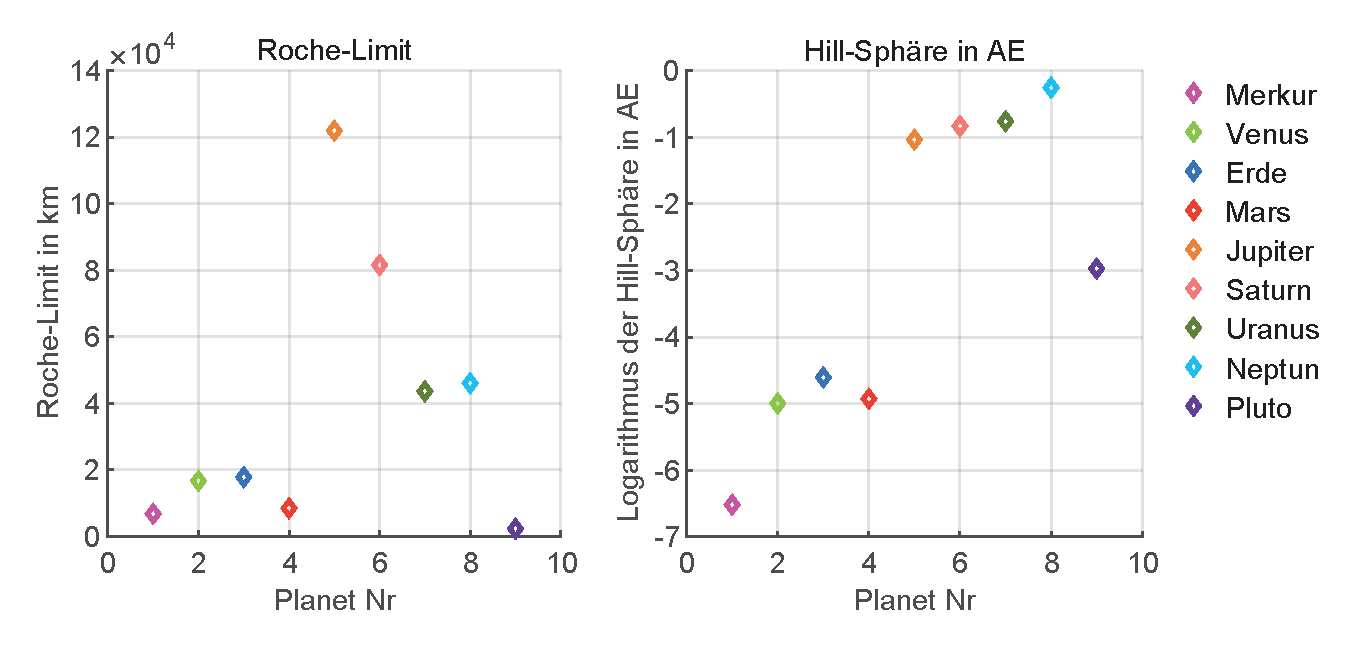
\includegraphics[width=\textwidth]{RocheLimit.pdf} 
	\caption[Vergleich Roche-Limit und Hill-Sph�re f�r unser Planetensystem.]{Vergleich Roche-Limit und Hill-Sph�re f�r unser Planetensystem.}
	\label{abb:hm_RocheLimit}
\end{figure}


\medskip \end{sol}
\textcolor{blue} {$\rightarrow$ zur} \probref{hm_rochelimit}.\\
\noindent\rule[1ex]{\textwidth}{0.5pt} \newpage


%-----------------------------------------------------------------------------------------------------------

\begin{sol} {prob:hm_gezeiten01} \label{lsg:hm_gezeiten01} %�bung33
\textbf{Tidenhub in einem Wasserglas}\\ \\

Wir betrachten \figref{hm_lsggezeiten01}. 
\begin{figure}[H]
	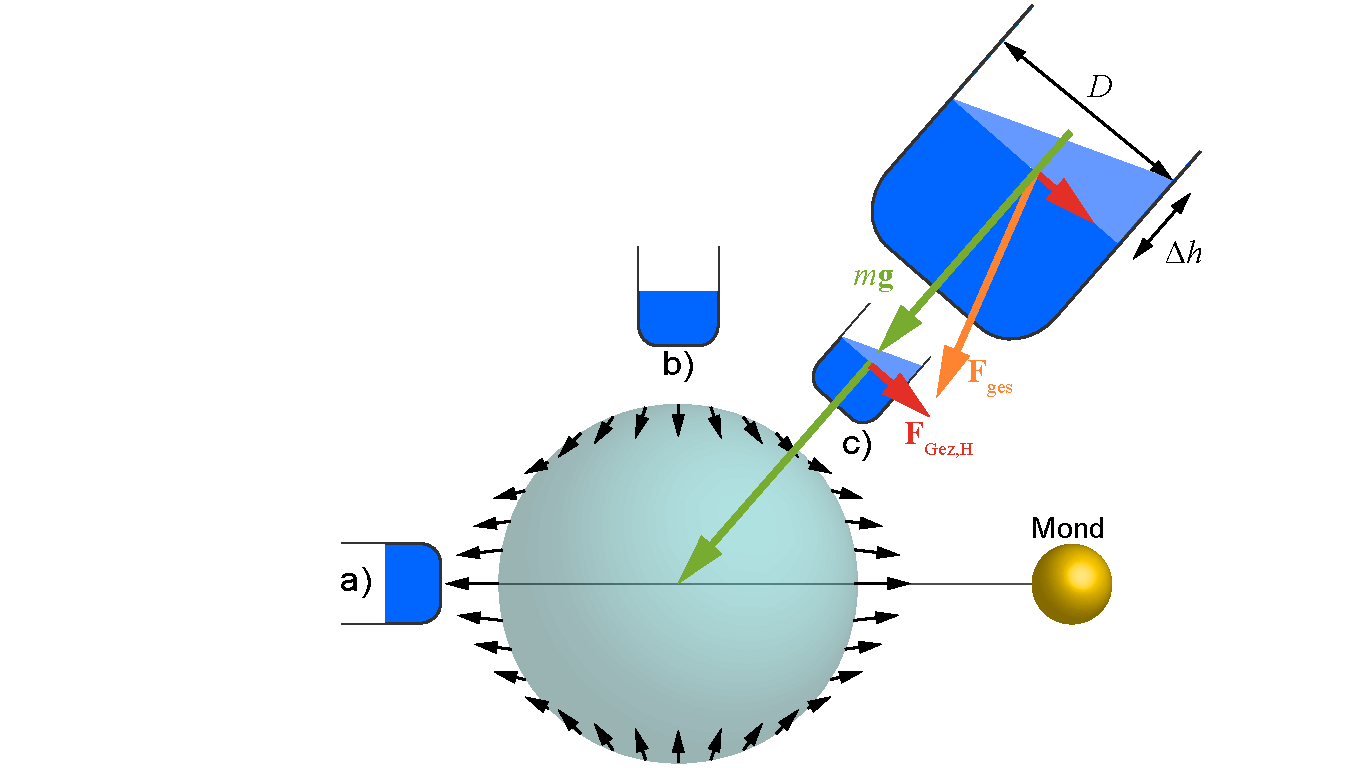
\includegraphics[width=\textwidth]{GezeitenWasserglas.pdf} 
	\caption{Gezeiten im Wasserglas}
	\label{abb:hm_lsggezeiten01}
\end{figure}
Nach der Gleichgewichtstheorie stellt sich die Wasseroberfl�che immer senkrecht zur resultierenden Gesamtschwerkraft $\vec{F}_\text{ges}$ ein. Der Tidenhub $\Delta h$ entspricht dann der Differenz der Wasserh�hen an beiden Ufern (\bzw dem R�ndern des Wasserglases). \\

Wir wollen nur die Wirkung des Mondes betrachten. Steht dieser im Zenit (Nadir) oder am Horizont, so bewirkt die resultierende Gesamtkraft keine Ver�nderung der Oberfl�che (Fall a,b). Im Fall c beginnt das Wasser durch Flie�en sich auszugleichen. \\
Der Tidenhub ergibt sich dann N�herungsweise zu:
\begin{align*}
    \Delta h = D\,\frac{F_\text{Gez,H}}{mg}\,.
\end{align*}
Wir wissen, dass $F_\text{Gez}/mg \approx \SI{e-7}{}$ ist, so dass folgt:
\begin{align*}
    \Delta h  &= \SI{e-8}{\metre} = \SI{10}{\nano\metre} ~~~~ \text{(Wasserglas)}, \\
    \Delta h  &= \SI{e-7}{}\cdot 5\cdot \SI{e4}{\metre} = 5\cdot \SI{e-3}{\metre} = \SI{5}{\mm} ~~~~ \text{(Bodensee)}.
\end{align*}

\newpage
Den Effekt im Glas k�nnte man im perfekt isolierten Labor ja noch interferometrisch messen, in der Badewanne oder aber im Bodensee wird er gegen�ber anderen Effekten verschwindend gering. 
In der Tat wurde die Wirkung von Gezeiten in $\SI{150}{\metre}$ langen Wasserrohren bereits 1914-1917 von Michelson\footnote{Albert Abraham Michelson (1852 -- 1931) war ein US-amerikanischer Physiker deutscher Herkunft. Er war einer der angesehensten Experimentalphysiker und wurde vor allem durch das nach ihm benannte Michelson-Interferometer bekannt. Er erhielt 1907 als erster US-Amerikaner den Nobelpreis f�r Physik.}\indexp{Michelson, Albert Abraham} und Mitarbeitern experimentell vermessen \cite{Michelson2014}.

\medskip \end{sol}
\textcolor{blue} {$\rightarrow$ zur} \probref{hm_gezeiten01}.\\
\noindent\rule[1ex]{\textwidth}{0.5pt} \newpage



%-----------------------------------------------------------------------------------------------------------

\begin{sol} {prob:hm_gezeiten02} \label{lsg:hm_gezeiten02} %�bung34
\textbf{Bewegung des Erdk�rpers im Erde-Mond-System.}\\

Der Umlauf von Erde und Mond um ihren gemeinsamen Schwerpunkt erzeugt oft Verwirrung. Oft wird argumentiert, dass die Erde dem Mond immer die gleich Seite zuwendet. Das ist aber falsch.
In der Realit�t f�hren alle Punkte der Erde eine Umlaufbewegung mit dem gleichen Radius aus und erfahren dabei eine gleiche Tr�gheitskraft (Fliehkraft), die immer vom Mond weg gerichtet ist. Jeder Punkt der Erde hat dabei sein eigenes Umlaufzentrum. Nur das gesamte System Erde-Mond f�hrt eine Bewegung um den Schwerpunkt S aus, nicht aber ein einzelner Massepunkt der Erde (Erde ist ja ein starrer K�rper).
Die \matlab{} Computersimulation \mlhmref{UmlaufErdeMond.m} zeigt in \figref{hm_lsggezeiten02}, dass jeder Punkt der Erde innerhalb eines synodischen Monats eine solche Kreisbewegung um sein jeweils eigenes "`Umlaufzentrum"' ausf�hrt. Dabei wurde die Situation f�r die �quatorebene dargestellt und angenommen, dass der Mond sich in der �quatorebene um den gemeinsamen Schwerpunkt S bewegt. Die Bewegung von zwei um $180\degree$ versetzten Punkten (T,B) in der �quatorebene sowie des Erdmittelpunktes im Lauf eines Monats sind dargestellt.

\newpage
\begin{figure}[H]
	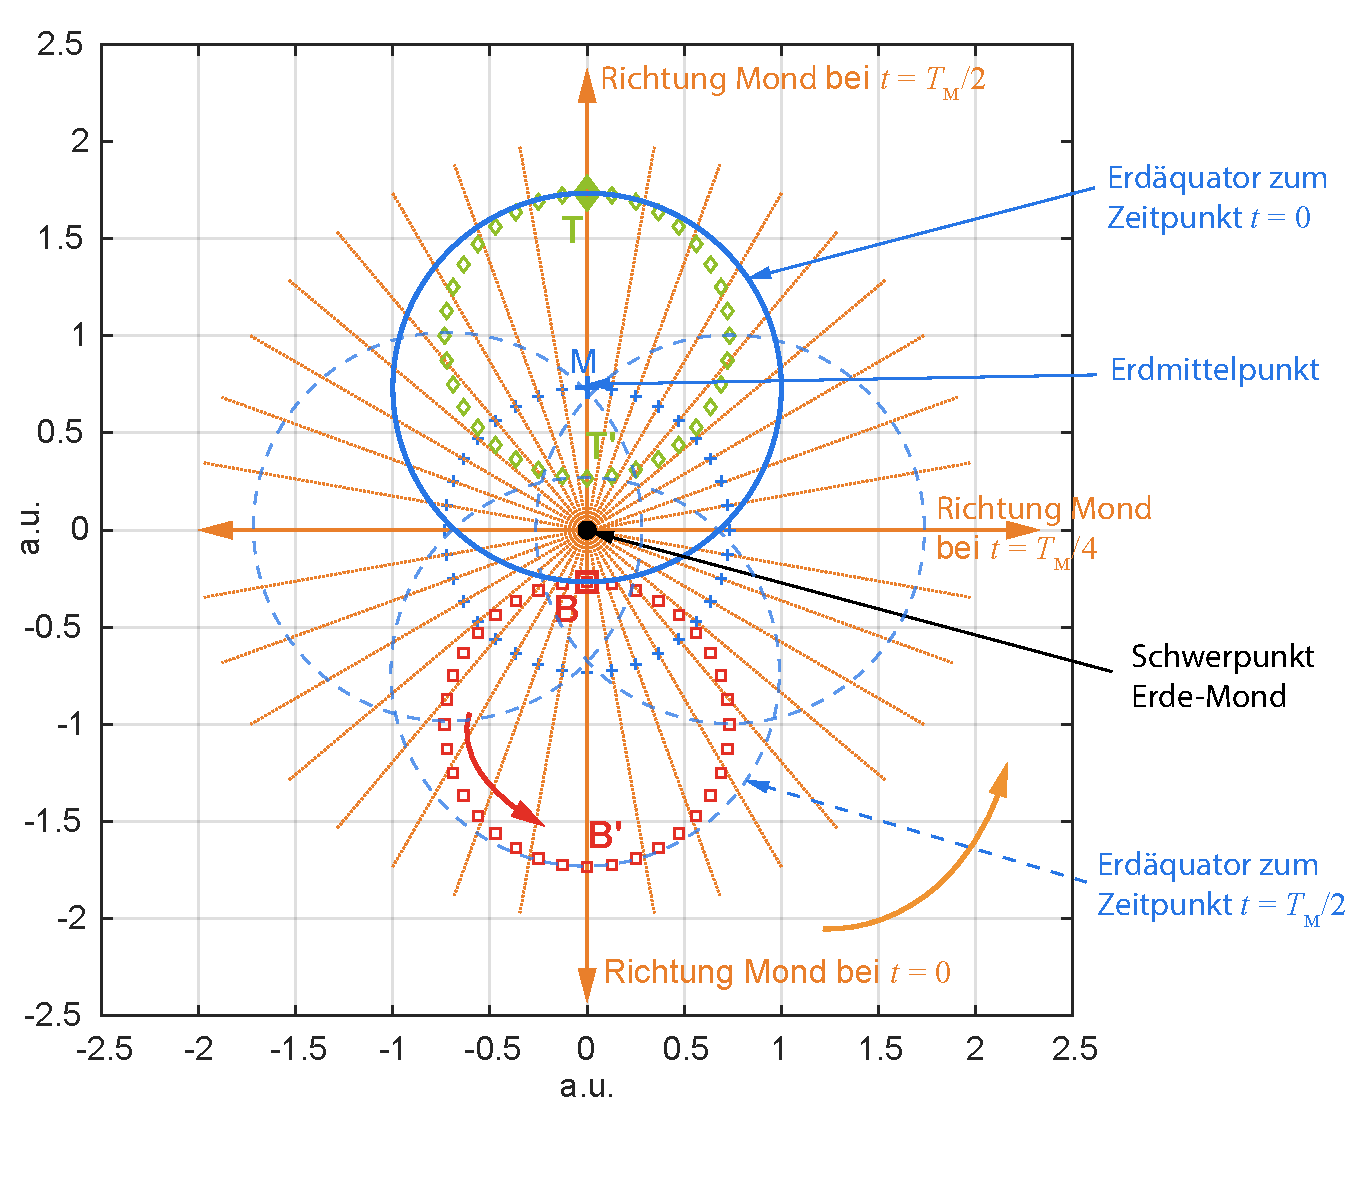
\includegraphics[width=\textwidth]{UmlaufErdeMond.pdf} 
	\caption[Bewegung von verschiedenen Punkten im Erde-Mond-System.]{Bewegung von verschiedenen Punkten der Erde bei einem Umlauf im Erde-Mond-Schwerpunkt-KOS. M ist der Erdmittelpunkt, T ein Punkt auf dem �quator, der bei $t=0$ auf der dem Mond abgewandten Seite liegt, T' der gleiche Punkt auf dem �quator, der bei $t=T_\text{M}/2$ dann auf der dem Mond zugewandten Seite liegt. F�r die Punkte B und B' gilt das Gleiche umgekehrt. $T_\text{M}$ ist die Umlaufzeit des Mondes um die Erde, die Erdrotation ist in dieser Betrachtung nicht ber�cksichtigt.}\label{abb:hm_lsggezeiten02}
\end{figure}
\end{sol}

\textcolor{blue} {$\rightarrow$ zur} \probref{hm_gezeiten02}.\\
\noindent\rule[1ex]{\textwidth}{0.5pt} \newpage

%-----------------------------------------------------------------------------------------------------------

\begin{sol} {prob:hm_gezeiten03} \label{lsg:hm_gezeiten03} %�bung35
\textbf{Newtonsche Gleichgewichtstheorie}\\ 

Abstand zwischen zwei Hochwassern und Tidenhub bei verschiedenen Deklinationen:
\begin{itemize}
	\item \textit{Abstand zwischen zwei Hochwassern }\\
			Aus der Dauer des synodischen Monats von $27.32 \mathrm{d}$ (Sonnentagen) ergibt sich eine mittlere Bewegung\index{Bewegung!mittlere} des Mondes von $n_\text{M} = 13.177\degree \mathrm{d}^{-1}$. An einem Sonnentag hat sich die Erde im Mittel um etwa 
	\[			360\degree \lk 1 + \frac{1\,\mathrm{d}}{365.25\,\mathrm{d}}\rk 
	\]
			weiter bewegt, was einer Bewegung von $n_\text{E} = 360.986\degree \mathrm{d}^{-1}$ entspricht. \\
			Wir wollen die zus�tzliche Zeit $\Delta T$ bestimmen, die verstreicht bis der Mond wieder im Meridian steht, \dh:
			\begin{align*}
					n_\text{E}\,\Delta T -360\degree &= n_\text{M} \, \Delta T \\
					\rightarrow ~~~~\Delta T = \frac{360\degree}{n_\text{E}-n_\text{M}} &= \frac{360\degree}{360.986\degree -13.177\degree}\, \mathrm{d} = \frac{360\degree}{347.809\degree}\, \mathrm{d} = 1.035 \mathrm{d} = \SI{24}{\hour}\,\SI{50}{\min}\,\SI{24}{\second}
			\end{align*}
			Hochwasser wird also im Mittel aller $\Delta T/2 = \SI{12}{\hour}\,\SI{25}{\min} $ eintreten.
			\begin{figure}%
			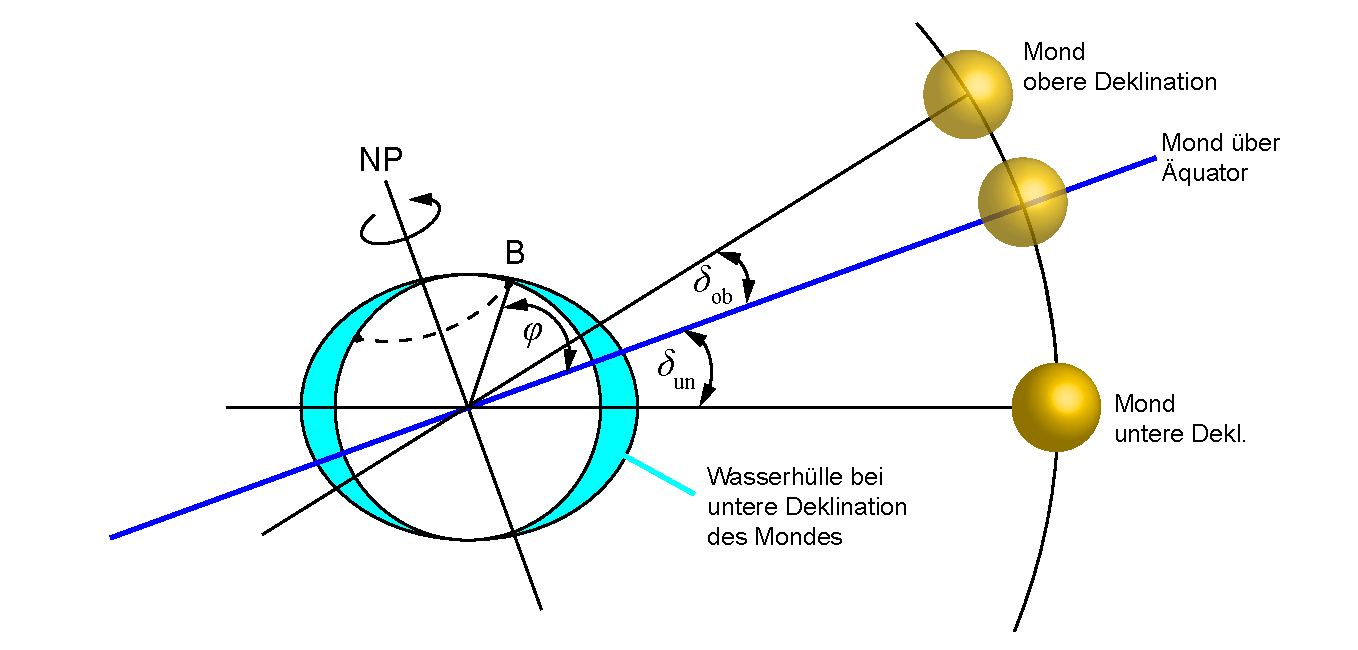
\includegraphics[width=\textwidth]{NewtonTheorieGez.pdf}%
			\caption{Anwendung der Newtonschen Gleichgewichtstheorie der Gezeiten}
			\label{abb:hm_lsggezeiten03}
			\end{figure}\newpage
	\item \textit{Tidenhub als Funktion der geographischen Breite }\\
	Man erkennt aus \figref{hm_lsggezeiten03}, dass die Tidenh�be f�r zwei aufeinander folgenden HW unterschiedlich hoch sind
	\item \textit{Tidenhub am �quator}\\
	Man erkennt aus \figref{hm_lsggezeiten03}, dass die Tidenh�be maximal sind, wenn der Mond die Deklination 0 hat. Ansonsten gibt es auch hier zwischen zwei aufeinander folgenden Hochwassern Unterschiede. Aus der Gezeitentabelle von Diego Garcia lesen wir heraus:
		\begin{enumerate}
		\item Sehr sch�n sind die Springtiden zum Vollmond und Neumond zu erkennen. (9.12. und 23.12.). Allerdings betr�gt die Differenz von HWH und NWH  \ca 250 cm, deutlich mehr als nach der Newtonschen Theorie zu erwarten w�re. Da zum Zeitpunkt des Vollmondes seine Deklination \ca $-10\degree$ betr�gt, die der Sonne \ca $-22\degree$ ist der Unterschied zwischen Tag- und Nachtiden entsprechend der unterschiedlichen Gezeitenwirkung ausgespr�gt. �hnliche Beobachtungen sind zur Neumondzeit zu machen.
		\item Der Mond kulminiert um \ca 9:00 Ortszeit, da finden wir aber NW, \dh wir haben fast eine Phasenverschiebung von $180\degree$, nach der Newtonschen Theorie nicht erkl�rbar.
		\item Die Nipptide am 15.12. ist gut ausgepr�gt, das Verh�ltnis von Spring- zu Nipptide von ca. 2.5 (250 cm / 100 m Tidenhub) entspricht grob der Newtonschen Theorie.
	\end{enumerate}
	\item
	  Die Nordsee ist ein sogenanntes Randmeer und bekommt daher die wesentlichen Gezeitenanregung vom Atlantik. Man kann sich die Nordsee als ein rechteckiges Becken von relativ geringer Tiefe (50 m) einer Breite/L�nge von etwa 1250 km vorstellen. Am Nordende dieses Beckens schwingen die Gezeitenwelle des Atlantiks mit Periode von $T = \SI{12}{\hour}\SI{25}{\minute}$ in das Becken nach S�den ein und werden an der Nordsee-S�dk�ste wieder reflektiert. Die Wellenl�nge berechnet sich aus $\lambda = c_\text{Welle} T = \sqrt{g\,h}\,T_\text{Gez}$ zu \ca 1000 km. Das Verh�ltnis zwischen Wellenl�nge und Beckenl�nge betr�gt somit etwa l : 1.25, bei diesem Schwingungsverh�ltnis bilden sich drei Schwingungsknoten aus (bei $\lambda=L$ w�ren es zwei.
    Durch die Coriolis-Kraft werden diese drei Schwingungsknoten zu ann�hernd station�ren amphidromischen Punkten, um die sich jeweils eine Welle im Gegenuhrzeigersinn bewegt. Man erkennt, dass diese amphidromischen Punkte nicht in der Mittelachse des Nordseebeckens liegen, sondern etwas nach Osten verschoben sind. Der Grund daf�r ist, dass die einlaufende Gezeitenwelle durch die geringe Tiefe der Nordsee stark abgebremst wird und so die wirkende Coriolis-Kraft Richtung S�den schw�cher wird. Diese asymmetrische Lage der amphidromischen Punkte ist f�r die unterschiedlich hohen Tidenh�be an Ost- und Westk�ste der Nordsee verantwortlich, da diese indirekt proportional zur Entfernung vom Amphidromiepunkt sind. (Je weiter weg, desto mehr kann sich die Gezeitenwelle aufbauen!).
\end{itemize}

\end{sol}
\textcolor{blue} {$\rightarrow$ zur} \probref{hm_gezeiten03}.\\
\noindent\rule[1ex]{\textwidth}{0.5pt} 

\begin{figure}%
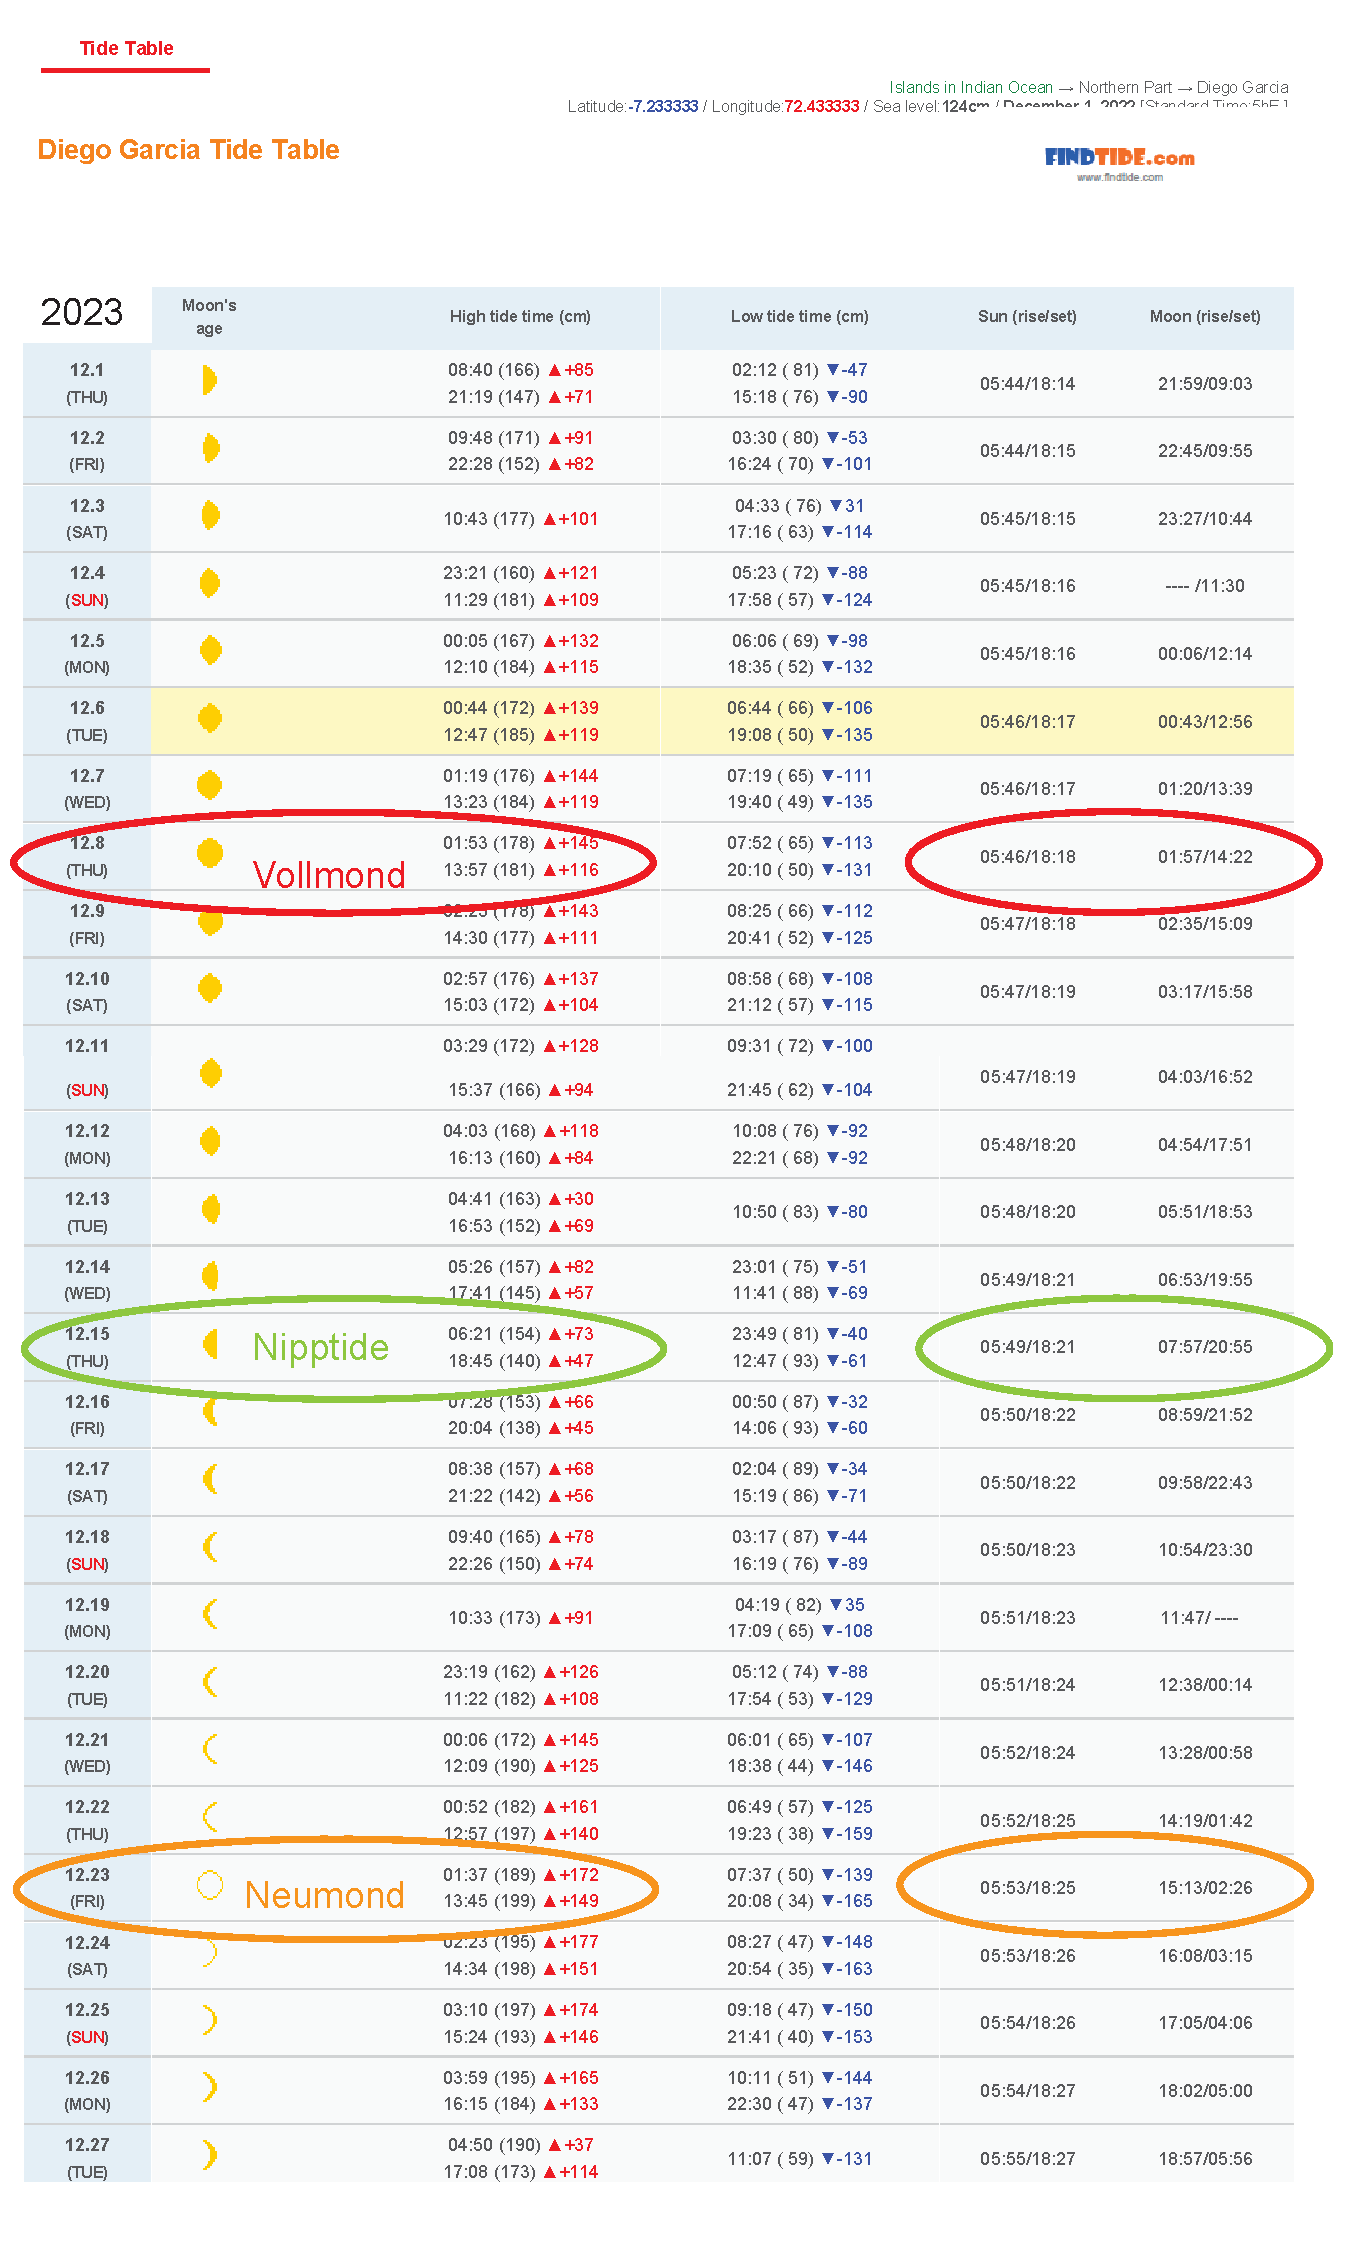
\includegraphics[width=\textwidth]{DiegoGarciaTideTableLsg.pdf}%
\caption{Tide Tabel von Diego Garcia im Indischen Ozean mit Beobachtungen}
	\label{abb:hm_DiegoGarciaTideTableLsg}
\end{figure}

\newpage

%-----------------------------------------------------------------------------------------------------------

\begin{sol} {prob:hm_gezeiten04} \label{lsg:hm_gezeiten04} %�bung36
\textbf{Gezeitenellipsoid}\\

\begin{itemize}
	\item \textit{\textbf{Newtonsche Gezeitentheorie}}\\ \\
	Wir verweisen auf \mlhmref{Gezeitenellipsoid.m}.

\begin{figure}[H]
	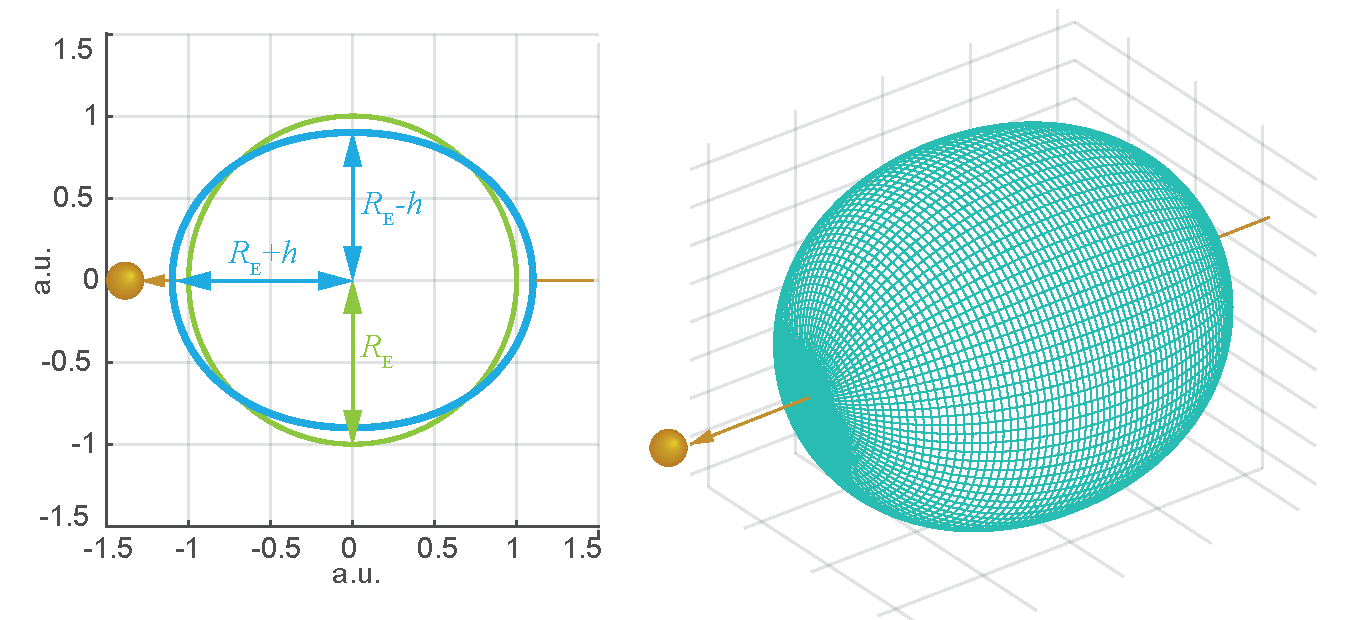
\includegraphics[width=\textwidth]{Gezeiten05.pdf} 
	\caption{Gezeitenellipsoid}
	\label{abb:hm_lsggezeiten04}
\end{figure}

F�r das Verh�ltnis der Volumina von Ellipsoid und Kugel finden wir :
	\[  \frac{V_\text{Ellip}}{V_\text{Kugel}} = \frac{(R_\text{E}+h)\,(R_\text{E}-h)^2}{R_\text{E}^3} \approx 1 - \frac{h}{R_\text{E}}  < 1\,,
	\]
was bedeutet, dass die angenommene Ellipsoidform nur eine N�herung sein kann. Eine verbesserte Rechnung m�sste sowohl die sogenannte Selbstgravitation des Gezeitenberges \cite{Norsen2017} als auch die Abflachungseffekte h�herer Ordnung sowie der bereits durch die Rotation der Erde hervorgerufene Abflachung \cite{Razmi2005} ber�cksichtigen.\\

	\item \textit{\textbf{Potentialtheorie}}\\ 

Wir benutzen \figref{hm_gezeiten02}. Das Potential der Gravitation des Mondes/der Sonne am Punkt $B$ ist gegeben durch: 
\begin{align*}
    U_\text{M} = -\frac{G\,m_\text{M}}{r'} ~~~~ \text{\bzw} ~~~~ U_\text{S} &= -\frac{G\,m_\text{S}}{r'}\,.
\end{align*}
Wir entwickeln $\vec{r}'= \vec{r} -\vec{R}$ wieder wie in \kap{hm_potentialtheorie} in sph�rischen Koordinaten $r,\theta$ (unter Ausnutzung der Rotationssymmetrie) und erhalten aus:
\begin{align}
    \frac{1}{r'} &= \frac{1}{\sqrt{r^2-2\vec{r}\,\vec{R} + R^2}} = \frac{1}{\sqrt{r^2-2r\,R\,\cos\theta+R^2}}  \label{eq:hm_lsggez31}\,.
\end{align}
Wir setzen jetzt $r= a_\text{EM}$ als festen Abstand der Mittelpunkte von der Erde und Mond und erhalten aus \eqref{eq:hm_lsggez31} wieder eine Entwicklung nach den Legendre-Polynomen analog zu \eqref{eq:hm_pot_theo07}
\begin{align}
    \frac{1}{r'} = \frac{1}{a_\text{EM}} \sum\limits_{n=0}^\infty \lk \frac{r}{a_\text{EM}}\rk^n\,\PL n\,\lk \cos\theta\rk\,. \label{eq:hm_lsggez32}
\end{align}
Daraus folgt mit $\mu_\text{M} = Gm_\text{M}$ das Potential am Punkt $B$ der Erdoberfl�che zu:
\begin{align}
    U_\text{M} = -\frac{\mu_\text{M}}{a_\text{EM}}\lek 1+\frac{r}{a_\text{EM}}\,\PL 1 \,\lk \cos\theta\rk + \frac{r^2}{{a_\text{EM}{}^2}}\,\PL 2 \,\lk\cos\theta\rk\rek\label{eq:hm_lsggez33}
\end{align}
und analog f�r die Sonne, wobei wir im Folgenden nun den Mond betrachten. \\
Der betrachtete Punkt $B$ erf�hrt im mitrotierenden Erde-Mond-System eine Zentrifugalkraft \bzw -Beschleunigung (siehe \probref{hm_gezeiten02})
\begin{align*}
    \vec{g}_\text{Z} &= -\omega_\text{M}{}^2\,\frac{m_\text{M}}{m_\text{M}+m_\text{E}} \,a_\text{EM}\,\vec{e}_\text{Z} \\
    &\approx -\omega_\text{M}\,\frac{m_\text{M}}{m_\text{E}}\,a_\text{EM}\,\vec{e}_\text{Z} = -\vec{\nabla}\,U_\text{Z}\,.
\end{align*}
Dies kann man mit \figref{hm_gezeiten02} als Potential
\begin{align}
    U_\text{Z} = \omega^2\,\frac{m_\text{M}}{m_\text{E}}\,a_\text{EM}\,r\,\cos\theta\label{eq:hm_lsggez34}
\end{align}
schreiben.\\
Wir benutzen, dass $\PL 1 \,\lk\cos\theta\rk = \cos\theta$ ist und erhalten mit $\omega^2 = \frac{\mu_\text{M}}{a_\text{EM}{}^3}$ (3. Keplersches Gesetz)
\begin{align}
    U_\text{Z} = \frac{\mu_\text{M}}{a_\text{EM}}\,\frac{r}{a_\text{EM}}\,\PL 1\,\lk\cos\theta\rk \label{eq:hm_lsggez35}\,.
\end{align}
Das gesamte auf den mitbewegten Punkt $B$ wirkende Potential ist dann die Summe von $U_\text{Z}$ und $U_\text{M}$, woraus folgt:
\begin{align}
    U = U_\text{Z} + U_\text{M} = -\frac{\mu_\text{M}}{a_\text{EM}}\,\lek 1+\frac{r^2}{a_\text{EM}{}^2}\,\PL 2\,\lk\cos\theta\rk\rek \,. \label{eq:hm_lsggez36}
\end{align}
Man erkennt aus \eqref{eq:hm_lsggez36}, dass sich die Terme, die linear in $r$ \bzw $\cos\theta$ sind, wegheben (bedingt durch die Balance von Gravitation und Zentrifugalkraft im rotierenden Erde-Mond-System) und dass als Zusatzterm zum Monopolpotential einer Punktmasse in 2. Ordnung das Gravitationspotential proportional zu $a_\text{EM}{}^{-3}$ �brig bleibt. \\ \\
Eine Fl�ssigkeit auf der Erdoberfl�che stellt sich in der H�he $h\lk\theta\rk$ und hat damit ein Potential $g\,h\lk\theta\rk$. Das gesamte Potential ist dann:
\begin{align}
    U_\text{total}\lk\theta\rk = -\frac{G\,m_\text{M}}{a_\text{EM}} + g\,h\lk\theta\rk- \zeta\,g\,\PL 2\,\lk\cos\theta\rk \label{eq:hm_lsggez37}
\end{align}
worin $\zeta$ durch
\begin{align*}
    \zeta = \frac{R_\text{E}{}^3}{a_\text{EM}{}^3}\,\frac{m_\text{M}}{m_\text{E}}\,R_\text{E}
\end{align*}
gegeben ist und wir $g= G\,m_\text{E}/r_\text{E}{}^2$ benutzt haben. \\
F�r eine Fl�ssigkeit muss das Potential $U$ unabh�ngig von $\theta$ sein, weil es sonst zu Ausgleichsstr�men kommt, womit sofort 
\begin{align}
    h\lk\theta\rk=\zeta\,\PL 2\,\lk\cos\theta\rk \label{eq:hm_lsggez38}
\end{align}
folgt und damit das bereits aus \eqref{eq:hm_gezeiten16} bekannte Ergebnis (bis auf konstante Terme).\\
In dieser Herleitung haben wir eine Fl�ssigkeit mit der Dichte $0$ unterstellt, die eine Erde die absolut fest ist komplett bedeckt. \\
Ein besseres Modell w�re sicher ein Zwei-Komponenten-Modell aus einem Planeten mit mittlerem Radius $R_\text{E}$, der einen homogenen inkompressiblen Ozean der Dichte $\rho_\text{W}$, einen homogenen, festen Kern der Dichte $\rho_\text{K}$ und eine Steifigkeit $\mu$ hat. Um dieses Modell zu berechnen, muss man die Effekte des Gravitationsfeldes des Gezeitenellipsoids selbst (die sogenannte Eigengravitation) und die der elastischen Kr�fte im Kern ber�cksichtigen. 
Wir verweisen %auf das erweiterte Problem in \probref{hm_gezeiten_zusatz} und 
die Spezialliteratur \cite{Murray2008,Norsen2017}.

\end{itemize}

\medskip \end{sol}
\textcolor{blue} {$\rightarrow$ zur} \probref{hm_gezeiten04}.\\
\noindent\rule[1ex]{\textwidth}{0.5pt} \newpage

%-----------------------------------------------------------------------------------------------------------

\begin{sol} {prob:hm_gezeiten05} \label{lsg:hm_gezeiten05} %�bung37
\textbf{Wasserkanal nach Airy \cite{Butikov2001}.}\\ \\

Einfaches Modell zur Dynamischen Theorie: 
Wir beziehen uns auf die instruktive Darstellung in \cite{Butikov2001}.
Wir betrachten den Airy-Wasserkanal entlang des �quators um die Erde und eine erzwungene Gezeitenschwingung (elliptischer Form) $q_1(t)$, deren Hauptachse auf die Erde-Mond-Linie ausgerichtet ist. Eine weitere Gezeitenschwingung (elliptischer Form), deren Hauptachse um $45\degree$ zur Erde-Mond-Linie verdreht ist, sei durch $q_2(t)$ gegeben. Die erzwungenen Wasserschwingungen im Kanal haben eine Eigenfrequenz $\omega_\text{Welle}$, die im Wesentlichen durch die Kanaltiefe bestimmt ist (siehe Band I) und die durch die halbt�gliche Gezeitenanregung mit $\omega_\text{Gez} = 2\,\omega_\text{E}$ erzwungen werden:
\begin{align*}
	\ddot{q}_1 +2\gamma\,\dot{q}_1 + \omega_\text{Welle}^2\,q_1 = A_1\,\omega_\text{Welle}^2\,\cos(\omega_\text{Gez}t) \,, \\
  \ddot{q}_2 +2\gamma\,\dot{q}_2 + \omega_\text{Welle}^2\,q_2 = A_2\,\omega_\text{Welle}^2\,\sin(\omega_\text{Gez}t)  \,.
\end{align*}
Hierin sind $\gamma$ die D�mpfungen und $A_, A_2 $ die Amplituden der Anregung der Gezeitenwellen.
Die Wasserh�hensteigung im Kanal an einer beliebigen Stelle des �quators (gegeben durch $R_\text{E},\, \theta$) ist dann gegeben durch:
	\[\Delta h = q_1\lk t\rk \cos 2\theta + q_2\lk t\rk \sin 2\theta \,.
	\]
F�r den Fall einer extrem langsam rotierenden Erde ist die Wasserh�hensteigung durch die station�re L�sung  $q_i(t)$ gegeben durch, wobei wir die Amplituden $A_1,\,A_2$ f�r beide Gezeitenwellen gleich annehmen wollen:
\begin{align}
   \Delta h &= q_1\lk t\rk \cos 2\theta + q_2\lk t\rk \sin 2\theta  \nonumber \\
    &= A\lek \cos\lk 2\omega_\text{Gez}t \rk \, \cos 2\theta + \sin \lk 2\omega_\text{Gez}t \rk \,\sin 2\theta \rek  \nonumber \\
    &= A\, \cos \lk 2\lk \omega_\text{Gez}t-\theta\rk\rk\,,  \label{eq:hm_gezeitenlsg01}
\end{align}
was bedeutet, dass die elliptischen Gezeitenverformungen der langsam rotierenden Erde folgen. Die Hauptachse der Gezeitenellipse ist immer auf die Erd-Mond-Linie ausgerichtet. \\
F�r beliebige $\omega_\text{E}$ benutzen wir als L�sung f�r die $q_i\lk t\rk$ die Berechnungen f�r den getriebenen Oszillator nach Gleichung (1.165) aus Kapitel 1.3.2 (Band I) mit der Amplitude
\begin{align*}
     \hat{q} &= \frac{\omega_\text{Gez}\,A}{\sqrt{\lk \omega_\text{Welle}{}^2\, - \,\omega_\text{Gez}{}^2\rk^2 + 4\gamma^2\,\omega_\text{Gez}{}^2}} \,,
\end{align*} 
und der Phase
\begin{align*}
    \delta &= \arctan\lek \frac{2\gamma\,\omega_\text{Gez}}{\omega_\text{Welle}{}^2 - \omega_\text{Gez}{}^2}\rek \,.
\end{align*} 
Daraus folgt nun f�r den Wasserh�henanstieg im Kanal:
\begin{align}
   \Delta h &= q_1\lk t\rk \cos 2\theta + q_2\lk t\rk \sin 2\theta  \nonumber \\
            &= \hat{q}\,\lek \cos\lk 2\omega_\text{E}t-\delta\rk\,\cos 2\theta + \sin\lk 2\omega_\text{E}t-\delta\rk\,\sin 2\theta\rek \nonumber \\
            &= \hat{q}\,\cos\lek 2\,\lk \omega_\text{E}t-\delta/2-\theta\rk\rek \,. \label{eq:hm_gezeitenlsg02}
\end{align}
Man erkennt aus \eqref{eq:hm_gezeitenlsg02}, dass der HW-Zeitpunkt an einer bestimmten Stelle des Erd�quators $R_\text{E},\, \theta$ gegeben ist durch:
\begin{align*}
    \theta_\text{max} = \omega_\text{E}\,t - \frac{\delta}{2}\,,
\end{align*}
was bedeutet, dass das Hochwasser mit einer bestimmten Zeitverschiebung  $\delta/2$ gegen�ber der Kulmination des Mond eintritt. Diese Verschiebung h�ngt von der Eigenfrequenz $\omega_\text{Welle}$ der Gezeitenwelle und ihrer D�mpfung $\gamma$ ab. In \figref{hm_lsggezeiten05} haben wir die �berlagerung und Verschiebung zur Erde Mond-Linie dargestellt.
Eine Simulation findet sich in \mlhmref{SimulationAiry.m}.

\begin{figure}[H]
	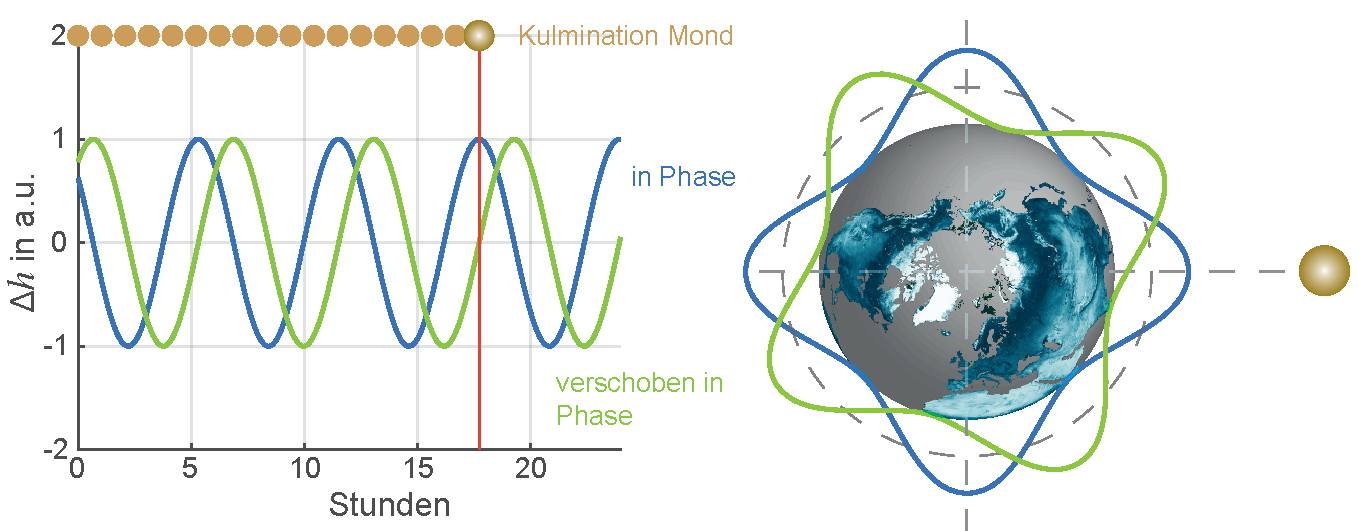
\includegraphics[width=\textwidth]{SimulationAiry.pdf} 
	\caption[Einfaches Modell zur Dynamischen Theorie.]{Einfaches Kanal-Modell nach Airy zur dynamischen Theorie der Gezeiten. Siehe auch \mlhmref{SimulationAiry.m}.
}
	\label{abb:hm_lsggezeiten05}
\end{figure}


\medskip \end{sol}
\textcolor{blue} {$\rightarrow$ zur} \probref{hm_gezeiten05}.\\
\noindent\rule[1ex]{\textwidth}{0.5pt} \newpage

%-----------------------------------------------------------------------------------------------------------

\begin{sol} {prob:hm_gezeiten06} \label{lsg:hm_gezeiten06} %�bung38
\textbf{Gezeitenreibung Hantelmodell}\\ \\

Die Rechnungen sind im Detail im \mscr{} \mlhmref{GezeitenReibung02.m} hinterlegt.
\begin{figure}[H]
	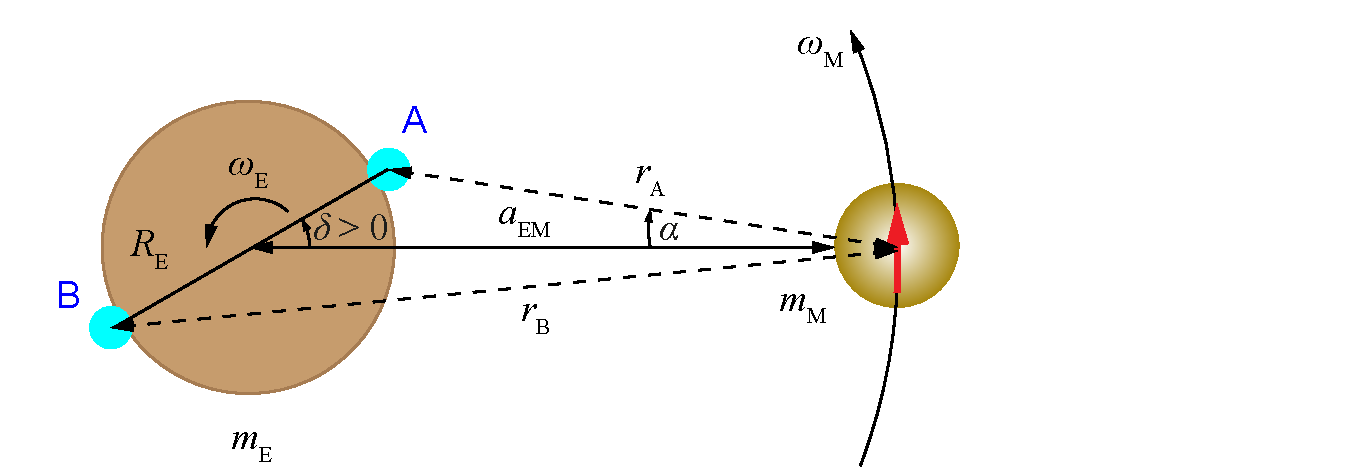
\includegraphics[width=\textwidth]{GezeitenHantel.pdf} 
	\caption{Gezeitenreibung - Hantelmodell}
	\label{abb:hm_lsggezeiten06}
\end{figure}
F�r die Berechnungen geben wir folgende Hinweise und Vorgehensweise zun�chst zur Ableitung des Drehmomentes aus \figref{hm_lsggezeiten06} an:
\begin{enumerate}
    \item [1)] Als erstes berechnen wir die Drehimpulse f�r den heutigen Zustand (Wir lassend dabei den Index 0 weg.):
    \begin{align*}
        L_\text{E} &= J_\text{E}\,\omega_\text{E}\,,~~ J_\text{E}\, \text{wird sp�ter berechnet}\,,~~~ \omega_\text{E} = \frac{2\pi}{\SI{86125}{\second}} \\
        L_\text{M} &= J_{\text{M}}\,\omega_\text{M} = m_\text{M}\,a_\text{EM}{}^2\,\omega_\text{M}\,, ~~~\omega_\text{M} = \frac{2\pi}{T_\text{synod.}}\,.
    \end{align*}
    %2)
    \item [2)] In der finalen Situation gilt: $\omega_\text{E,f} = \omega_\text{M,f}$:
    \begin{align*}
        L_\text{E,f} &= J_\text{E}\,\omega_\text{E,f}~,~~  L_\text{M,f} = J_\text{M,f}\,\omega_\text{M,f} = m_\text{M}\,a_\text{EM,f}{}^2\,\omega_\text{M,f}\,.
		\end{align*}
    %3)
    \item [3)] Aus der Drehimpulserhaltung folgt:
    \begin{align*}
        L_\text{ges} = J_\text{E}\,\omega_\text{E} + J_\text{M}\,\omega_\text{E} = J_\text{E}\,\omega_\text{E,f} + J_\text{M,f}\,\omega_\text{M,f}\,
    \end{align*}
und mit
    \begin{align*}
        \omega_\text{E,f} &= \omega_\text{M,f} ~~\rightarrow~~J_\text{E}\,\omega_\text{E} + J_\text{M}\,\omega_\text{M} = \lk J_\text{E} + J_\text{M,f}\rk\,\omega_\text{M,f}\,.
    \end{align*}
    Wir vergleichen:
    \begin{align*}
        J_\text{E} &\approx \frac{2}{5}\,m_\text{E}\,R_\text{E}{}^2\,~~\text{und}~~ J_\text{M,f} > J_\text{M} = m_\text{M}\,a_\text{EM}{}^2 ~\rightarrow~
        \frac{J_\text{E}}{J_\text{M}} = \frac{2}{5}\,\frac{m_\text{E}}{m_\text{M}}\,\frac{R_\text{E}{}^2}{a_\text{EM}{}^2} = 0.0045 \ll 1\,.
    \end{align*}
    Deswegen k�nnen wir in guter N�herung $J_\text{E} \ll J_\text{M,f}$ annehmen, womit folgt:
    \begin{align}
        L_\text{ges} = J_\text{E}\,\omega_{\text{E}} + J_\text{M}\,\omega_\text{E} = J_\text{M,f}\,\omega_\text{M,f} \label{eq:hm_gezUebg01} \,.
    \end{align}
    %4)
    \item[4)] Wir bestimmen nun den endg�ltigen Erde-Mond-Abstand $a_\text{EM,f}$ und die endg�ltige Kreisfrequenz $\omega_\text{M,f}$. Dazu betrachten wir die Kr�ftebilanz im finalen Zustand:
    \begin{align}
        \frac{G\,\killA{m_\text{M}}\,m_\text{E}}{a_\text{EM,f}{}^2} = \killA{m_\text{M}}\,\omega_\text{M,f}{}^2\,a_\text{EM,f} \label{eq:hm_gezUebg02} \,.
    \end{align}
    Aus \eqref{eq:hm_gezUebg01} und \eqref{eq:hm_gezUebg02} folgt
    \begin{align}
        a_\text{EM,f} &= \frac{L_\text{ges}{}^2}{G\,m_\text{E}\,m_\text{M}{}^2} \label{eq:hm_gezUebg03} \\
        \omega_\text{M,f} &= \frac{L_\text{ges}}{m_\text{M}\,a_\text{EM,f}{}^2} = \frac{G^2\,m_\text{E}{}^2\,m_\text{M}{}^3}{L_\text{ges}^3}\,. \label{eq:hm_gezUebg04}
    \end{align}
    %5)
    \item [5)] Zur Berechnung von $L_\text{ges}$ brauchen wir noch das Tr�gheitsmoment der Erde. \\
    Wir wollen die Erde aus einem Kern mit Dichte $\varrho_\text{K}$ und Radius $R_\text{K}$ und einer Schale $\varrho_\text{S}$ im Radiusbereich $R_\text{U}$ bis $R_\text{E}$ annehmen.
    \begin{align*}
        J_\text{E} &= \frac{2}{5}\,\lk \frac{4}{3}\,\pi\,\varrho_\text{S}\,R_\text{E}{}^3\rk\,R_\text{E}{}^2 + \frac{2}{5}\,\lk \frac{4}{5}\pi\,\lk \varrho_\text{K}-\varrho_\text{S}\rk\,R_\text{K}{}^3\rk\,R_\text{K}{}^2 \\
        &= \frac{2}{3}\,\frac{4}{3}\,\pi\lek \varrho_\text{S}\,R_\text{E}{}^5 + \varrho_\text{K}\,R_\text{K}{}^5 - \varrho_\text{S}\,R_\text{K}{}^5\rek = \frac{8}{15}\,\pi\lek \varrho_\text{S}\,\lk R_\text{E}{}^5 -R_\text{K}{}^5\rk + \varrho_\text{K}\,R_\text{K}{}^5\rek \\
        &\approx \SI{7.83e37}{\kg\square\metre}\\
        \text{\vgl homogene Erde} ~~~~ J_\text{EK} &= \frac{8}{15}\,\pi\,\varrho_\text{E}\,R_\text{E}{}^5 = \SI{9.7e37}{\kg\square\metre} \,.
    \end{align*}
    %6)
    \item[6)] Damit erhalten wir
    \begin{align*}
        L_\text{ges} &= J_\text{E}\,\omega_\text{E} + J_\text{M}\,\omega_\text{M} \approx \SI{3.45e34}{\kg\square\metre\per\second}\,.
    \end{align*}
    %7)
    \item[7)] Aus \eqref{eq:hm_gezUebg03} und \eqref{eq:hm_gezUebg04} erhalten wir:
    \begin{align*}
        a_\text{EM,f} &= \SI{5.55e8}{\km} = 1.44\,a_\text{EM}\,~~\text{und}~~ \omega_\text{M,f} = \SI{1.528e-6}{\per\second} ~~\rightarrow ~~T_\text{E,f} = \frac{2\pi}{\omega_\text{M,f}} = \SI{47.59}{}~\mathrm{d}\,.
    \end{align*}
    %8)
   \item [8)] Jetzt wollen wir noch wissen, wie lange es dauert bis der finale Zustand erreicht ist, \bzw um welche Distanz sich der Mond pro Jahrhundert entfernt. Nach \figref{hm_lsggezeiten06} ist:
    \begin{align*}
        F_\text{A} = \frac{G\,m\,m_\text{M}}{r_\text{A}{}^2} &= \frac{G\,m\,m_\text{M}}{a_\text{EM}{}^2 + R_\text{E}{}^2 - 2a_\text{EM}\,R_\text{E}\,\cos\delta} \\
        F_\text{B} = \frac{G\,m\,m_\text{M}}{r_\text{B}{}^2} &= \frac{G\,m\,m_\text{M}}{a_\text{EM}{}^2 + R_\text{E}{}^2 - 2a_\text{EM}\,R_\text{E}\,\cos\lk 180\degree-\delta\rk} \\
        &= \frac{G\,m\,m_\text{M}}{a_\text{EM}{}^2 + R_\text{E}{}^2 + 2a_\text{EM}\,R_\text{E}\,\cos\delta }
    \end{align*}
    Die Drehmomente auf die Hantel ergeben sich f�r kleine Winkel $\delta$ und $\alpha\approx 0$ zu:
    \begin{align*}
						\vec{M}_\text{D, A} &= \vec{R}_\text{E} \times \vec{F}_\text{A}\\
						M_\text{D, A}  &= R_\text{E}\,F_\text{A}\,\lk -\cos\delta\,\sin\alpha - \sin\delta\,\cos\alpha \rk \\
						\sin\delta &\approx \delta,~~\alpha \approx \frac{R_\text{E}}{r_\text{A}}\delta~\text{Sinussatz}\,~~~ \cos\alpha \approx 1,~~ \cos\delta \approx 1\,,\\
						M_\text{D, A}  &= +R_\text{E}\,F_\text{A}\,\delta \lk 1 + \frac{R_\text{E}}{r_\text{A}} \rk \,,~~
						M_\text{D, B}  = -R_\text{E}\,F_\text{B}\,\delta \lk 1 - \frac{R_\text{E}}{r_\text{A}} \rk \,, \\
						\rightarrow ~~M_\text{D, ges}&\approx -R_\text{E}\delta \lk F_\text{A} - F_\text{B} \rk \,.
			\end{align*}
    F�r das Gesamtdrehmoment auf die Hantel nehmen wir f�r $m$  \ca $\SI{e-8}{}$ $m_\text{E}$ an (wegen $g_\text{gez}|g_\text{E}$) also $m\approx\SI{3.8e-16}{\kg}$, $\delta = 3\degree$ 
    \begin{align*}
        \rightarrow ~~~~  M_\text{D, ges} &= \SI{-4.39e16}{\N\metre}
    \end{align*}
    %9)
    \item[9)] 
		Die Bewegungsgleichung f�r den starren K�rper ergibt:
    \begin{align*}
        -\frac{\D L}{\D t}\,M &=  M_\text{D, ges} = \frac{\D L_\text{E}}{\D t} = J_\text{E}\,\dot{\omega}_\text{E} = \frac{\D }{\D t}\,\lk m_\text{M}\,\omega_\text{M}\,a_\text{EM,f}{}^2\rk
    \end{align*}
    Aus der Drehimpulserhaltung folgt:
    \begin{align*}
				L &= \frac{2}{5}\,m_\text{E}\,R_\text{E}{}^2\,\omega_\text{E} + m_\text{M}\,a_\text{EM}{}^2\,\omega_\text{M} \\
				\frac{\D L}{\D t} = 0 &= \frac{2}{5}\,m_\text{E}\,R_\text{E}{}^2\,\dot{\omega}_\text{E} + 2m_\text{M}\,a_\text{EM}\,\dot{a}_\text{EM}\,\omega_\text{M} + m_\text{M}\,a_\text{EM}{}^2\,\dot{\omega}_\text{M} ~~~~ \Bigg|\substack{:\lk 2m_\text{M}\,a_\text{EM}{}^2\,\omega_\text{M} \rk}\\					0 &= \frac{1}{5}\,\frac{m_\text{E}\,R_\text{E}{}^2}{m_\text{M}\,a_\text{EM}{}^2}\,\frac{\dot{\omega}_\text{E}}{\omega_\text{M}} + \frac{\dot{a}_\text{EM}}{a_\text{EM}} + \frac{1}{2}\,\frac{\dot{\omega}_\text{M}}{\omega_\text{M}} \\
					\omega_\text{M} &= \sqrt{G\,m_\text{M}}\,a_{EM}{}^{-\frac{3}{2}} ~~~~ \rightarrow ~~~~ \dot{\omega}_\text{M} = \sqrt{G\,m_\text{M}}\,\lk -\frac{3}{2}\rk\,a_\text{EM}{}^{-\frac{5}{2}}\,\dot{a}_\text{EM} = -\frac{3}{2}\,\frac{\dot{a}_\text{EM}}{a_\text{EM}}\,\omega_\text{M} \\
				\rightarrow ~~~~ &-\frac{1}{5}\,\frac{m_\text{E}\,R_\text{E}{}^2}{m_\text{M}\,a_\text{EM}{}^2}\,\frac{\dot{\omega}_\text{E}}{\omega_\text{M}} = \frac{\dot{a}_\text{EM}}{a_\text{EM}}\,\lk 1-\frac{1}{2}\,\frac{3}{2}\rk \\
				\rightarrow ~~~~ &\frac{\dot{a}_\text{EM}}{a_\text{EM}} = -\frac{4}{5}\,\frac{m_\text{E}\,R_\text{E}{}^2}{m_\text{M}\,a_\text{EM}{}^2}\,\frac{\dot{\omega}_\text{E}}{\omega_\text{M}}\\
        \rightarrow ~~~~ &\dot{\omega_\text{E}} = \frac{M_\text{ges}}{J_\text{E}} \approx \SI{-5.61e-22}{\per\square\second} \,, \\
        \rightarrow ~~~~ &\dot{a}_\text{EM} = -2\,\frac{J_\text{E}\,\dot{\omega}_\text{E}}{m_\text{M}\,a_\text{EM}\,\omega_\text{M}} \approx \SI{1.17e-9}{\metre\per\second}\,.
    \end{align*}
    Umgerechnet bedeutet das f�r 100 Jahre:
    \begin{align*}
        \Delta T_\text{PE} &= -\frac{\dot{\omega}_\text{E}}{2\pi}\,T_\text{PE}{}^2\, \underbrace{100 \cdot 365 \cdot 86400}_{\substack{=100\,\mathrm{a}}} \SI{}{\second} = -\frac{\dot{\omega}_\text{E}}{\omega_\text{E}{}^2}\,2\pi\, 100\,\mathrm{a} \approx \SI{0.0021}{} \SI{}{\second} = \SI{2.1}{\metre\second}\,, \\
        \Delta a_\text{EM} &= \dot{a}_\text{EM}\, 100\,\mathrm{a} \approx \SI{3.7}{\metre}\,.
    \end{align*}
    %10)
\end{enumerate}

Jetzt wollen wir uns noch die Energiebilanz anschauen. Wir geben auch dazu die Vorgehensweise an:
    \begin{align*}
         E_\text{ges} &= \frac{J_\text{E}}{2}\,\omega_\text{E}{}^2 + \frac{J_\text{M}}{2}\,\omega_\text{M}{}^2 - \frac{G\,m_\text{M}\,m_\text{E}}{a_\text{EM}}\,,\\
         E_\text{ges} &= \frac{J_\text{E}}{2}\,\omega_\text{E}{}^2 + \frac{J_\text{M}}{2}\,\frac{G\,m_\text{E}}{a_\text{EM}{}^3} - \frac{G\,m_\text{M}\,m_\text{E}}{a_\text{EM}}\,, \\
        \rightarrow\frac{\D E}{\D t} &= J_\text{E}\,\omega_\text{E}\,\dot{\omega}_\text{E} - \frac{3}{2}\,\frac{J_\text{M}\,G\,m_\text{E}}{a_\text{EM}{}^4}\,\dot{a}_\text{EM} + \frac{G\,m_\text{E}\,m_\text{M}}{a_\text{EM}{}^2} \,\dot{a}_\text{EM} = P_\text{V} \approx \SI{-3.3e12}{\W}\,.
    \end{align*}
    Wir berechnen die \anf{Arbeit}, die die Gravitationsenergie beim Anheben der Ozeane leistet (pro Tag). Dazu brauchen wir zun�chst die Masse $m_\text{W}$ der angehobenen Wasserschicht:
    \begin{align*}
        m_\text{W} &= \frac{4}{3}\,\pi\,\lk R_\text{E} +h\rk^3\,\varrho - \frac{4}{3}\,\pi\,R_\text{E}\,\varrho = \frac{4}{3}\,\pi\,\varrho\,R_\text{E}{}^3\,\lk 1 + \frac{3h}{R_\text{E}} + \killA{\mathcal{O} \lk \frac{h^2}{R_\text{E}{}^2}\rk}\rk \,,\\
        \rightarrow ~ E_\text{W} &= -2m_\text{W}\,g\,h = \SI{-2.5e18}{\W} \,,\\
        P_\text{Diss} = \dot{E}_\text{Diss} &= -10\% \, \frac{E_\text{W}}{\SI{24}{\hour}} = \SI{-2.9e12}{\W} \,, \\
        E_\text{Diss} \lk 1a\rk &= P_\text{Diss} \, 1a = \SI{-25.4}{\peta\W\hour} = \SI{-25.4e4}{\tera\W\hour} \,.
    \end{align*}
    Wir vergleichen das mit dem weltweiten Prim�renergieverbrauch 2021 von 600 ExaJoule = $\SI{1.67e5}{\tera\W\hour}$, was bedeutet, dass die Gezeitenreibungs-Verlustenergie etwa $10\%$ des weltweiten Prim�renergieverbrauchs betr�gt. Wir k�nnen noch absch�tzen, zu welcher Erw�rmung der Ozeane das f�hrt, falls keine Abstrahlung ins Weltall erfolgen w�rde.
    \begin{align*}
        E_\text{Diss}\lk 1a\rk &= m_\text{W}\,c\,\Delta T~,~~~c_\text{W} = \SI{4.2}{}\,\frac{\SI{}{\kilo\J}}{\SI{}{\kg\K}}\,,\\
        \Delta T_\text{W} &= \frac{E_\text{Diss}\lk 1a\rk}{m_\text{W}\,c_\text{W}} \approx \SI{0.8}{\K} \,.
     \end{align*}

\medskip \end{sol}
\textcolor{blue} {$\rightarrow$ zur} \probref{hm_gezeiten06}.\\
\noindent\rule[1ex]{\textwidth}{0.5pt} \newpage

%-----------------------------------------------------------------------------------------------------------

\begin{sol}{prob:hm_gezeiten06a}\label{lsg:hm_gezeiten06a} %�bung39
\textbf{Gezeitenreibung - Auswirkung Mond.}\\ \\

Wir k�nnen die gleichen Gedankeng�nge wie im \kap{hm_gezeitenreibung} machen und erhalten die entsprechenden Gleichungen angepasst f�r den Mond.\\
Insbesondere ergibt \eqref{eq:hm_gezreibung08} nun:
\begin{align*}
    \frac{\dot{\Omega}_\text{M}}{\Omega_\text{M}} &= -\frac{45}{4}\,\frac{\omega_\text{M}{}^2}{\omega_\text{M}}\,\frac{m_\text{E}}{m_\text{M}}\,\lk \frac{R_\text{M}}{a_\text{EM}}\rk^3\,\frac{\delta}{1+\tilde{\mu}} \\
    &\approx \SI{1.1e-14}{\per\second}
\end{align*}
Die Zeitdauer, in der der Mond auf eine synchrone Eigenrotation gekommen ist, betr�gt dann
\begin{align*}
    \Delta T \approx \Big|\frac{\Omega_\text{M}}{\dot{\Omega}_\text{M}}\Big| \approx \SI{3e6}{} \text{Jahre}\,.
\end{align*}
Im Vergleich zum angenommenen Mondalter von ca. 4.5 Milliarden Jahren ist das eine verschwindend kurze Zeit. Daher ist es kaum �berraschend, dass der Mond schon lange eine synchrone Rotation zur Erde hat und uns immer das gleiche Gesicht zeigt.

\medskip \end{sol}
\textcolor{blue} {$\rightarrow$ zur} \probref{hm_gezeiten06}.\\
\noindent\rule[1ex]{\textwidth}{0.5pt} \newpage

%-----------------------------------------------------------------------------------------------------------

\begin{sol}{prob:hm_gezeiten07}\label{lsg:hm_gezeiten07} 
\textbf{Gravitationspotential au�erhalb eines Rotationsellipsoids.}\\ %�bung40

Wir nehmen die Form des homogenen Rotationsellipsoids mit
\begin{align}
    r'\lk \theta'\rk = R_0\lk 1-\frac{2}{3}\,\epsilon\,\PL 2\,\lk \cos\theta'\rk\rk \label{eq:hm_rotell01}
\end{align}
an, wobei $|\epsilon|\ll 1$ sein soll. \\
Nach \eqref{eq:hm_pot_theo07} in \kap{hm_pot_rotsymm_distrib} k�nnen wir das Potential an einem Ort $r,\, \theta$ vschreiben als:
\begin{align}
    U\lk r,\theta\rk = \sum_{n=0}^\infty \Phi_n\,\frac{\PL n \,\lk \cos\theta\rk}{r^{n+1}}\,, \label{eq:hm_rotell02}
\end{align}
worin
\begin{align}
    \Phi_n = -2\pi\,G\,\int\limits_0^\pi\int\limits_0^{r'\lk\theta'\rk}\,r'^{2+n}\,\varrho\lk r',\theta'\rk\,\PL n\lk\cos\theta'\rk \,\sin\theta'\,\D r'\,\D \theta'\,. \label{eq:hm_rotell03}
\end{align}
Das Integral ist �ber die gesamte Masseverteilung desK�rpers zu nehmen. \\
F�r einen homogenen K�rper der Dichte $\varrho$ k�nnen wir schreiben:
\begin{align}
    \Phi_n = -2\pi\,G\,\varrho\int\limits_0^\pi \PL n\,\lk\cos\theta'\rk \int\limits_0^{r'\lk \theta'\rk}r'^{2+n}\,\D r' \,\sin\theta'\,\D \theta'\,. \label{eq:hm_rotell04}
\end{align}
Die Integration �ber $r'$ ergibt:
\begin{align}
    \Phi_n = -\frac{2\pi\,G\,\varrho}{\lk n+3\rk}\int\limits_0^\pi \PL n\,\lk\cos\theta'\rk \,\lek r'\lk\theta'\rk\rek^{n+3}\,\sin\theta'\,\D \theta' \label{eq:hm_rotell05}\,,
\end{align}
in welches wir \eqref{eq:hm_rotell01} einsetzen und somit erhalten:
\begin{align}
    \Phi_n\approx -\frac{2\pi\,G\,\varrho}{\lk n+3\rk} \int\limits_0^\pi \PL n\,\lk \cos\theta'\rk R_0{}^{n+3}\,\lek \PL 0\lk\cos\theta'\rk - \frac{2}{3}\,\lk n+3\rk\,\epsilon\,\PL 2\lk\cos\theta'\rk\rek\,\sin\theta'\,\D \theta'\,. \label{eq:hm_rotell06}
\end{align}
Hier haben wir f�r $|\epsilon|\ll 1$\, $\lk 1+\epsilon\, x\rk^{n+3} \approx 1 + \lk n+3\rk\,\epsilon\, x$ und ferner $\PL 0\,\lk \cos\theta'\rk = 1$ benutzt.\\
Wegen der Orthogonalit�t der Legendre-Polynome (siehe \cite{Riley2006, Olver1992, Fischer2018} und die \onlineZ) k�nnen nur $\Phi_0$ und $\Phi_2$ von Null verschieden sein. Wir erhalten:
\begin{align}
\begin{split}
    \Phi_0 &= -\frac{4\pi\,G\,\varrho\,R_0{}^3}{3} = -G\,M\,, \\
    \Phi_2 &= \frac{8\pi\,G\,\varrho\,R_0{}^5\,\epsilon}{15} = \frac{2}{5}\,G\,M\,R_0{}^2\,\epsilon\,,
\end{split} \label{eq:hm_rotell07}
\end{align}
wobei wir mit $M = \frac{4\pi}{3}\,R_0{}^3\,\varrho$ die Masse der homogenen Kugel mit dem mittleren Radius $R_0$ bezeichnet haben.\\
Das Potential ergibt sich damit zu:
\begin{align*}
    U = U_0+U_2
\end{align*}
mit
\begin{subequations}
\begin{align}
      U_0 &= -\frac{G\,M}{r} \label{eq:hm_rotell08a} \,,\\
      U_2 &= \frac{2}{5}\,\frac{G\,M}{r^3}\,R_0{}^2\,\epsilon\,\PL 2\lk \cos\theta\rk \,.\label{eq:hm_rotell08b}
\end{align}
\end{subequations}
Man vergleiche diese Beziehung auch \eqref{eq:hm_rotell08b} mit dem Ansatz, welchen wir im Kapitel 1.5.5 im Band I f�r Herleitung der Frequenz der Pr�zessions der Erdachse im Gravitationsfeld des Mondes/der Sonne benutzt hatten.\\

\medskip \end{sol}
\textcolor{blue} {$\rightarrow$ zur} \probref{hm_gezeiten07}.\\
\noindent\rule[1ex]{\textwidth}{0.5pt} \newpage


%-----------------------------------------------------------------------------------------------------------

\begin{sol}{prob:hm_gezeiten09}\label{lsg:hm_gezeiten09} %�bung41
\textbf{Vergleich Gravitationseffekte auf die Erde}\\ \\

In \figref{hm_lsggezeiten10} und Tabelle \ref{tab:hm_Vergleich} haben wir die wesentlichen Charakteristika der Effekt zusammengefasst.

\begin{figure}[H]
	\includegraphics[width=\textwidth]{VergleichEffekte.pdf} 
	\caption{Vergleich verschiedener Effekte der Himmelsmechanik auf unsere Erde}
	\label{abb:hm_lsggezeiten10}
\end{figure}


\begin{sidewaystable}
\vspace{12cm}
\caption{Vergleich Gravitationseffekte auf die Erde} \label{tab:hm_Vergleich}
\begin{center}
\smallskip
%\begin{adjustbox}{width=\textwidth,totalheight=0.5\textheight,keepaspectratio}
\begin{tabular}{L{2.5 cm}L{2.5cm}L{2.6cm}L{5.5cm}L{4.5cm}}
\hline\noalign{\smallskip}
Effekt& KOS & Kr�fte \linebreak Drehmomente & Gr��enordnung Effekt & Charakteristische Werte \\
\noalign{\smallskip}\svhline\noalign{\smallskip}
Rotationsabplattung & Rotierendes System der Erde \linebreak Mitbewegter Beobachter & Zentrifugalkraft &$f = \frac{\omega_\text{E}{}^2\, R_\text{E}}{2\, g_\text{E}}$ & $f \approx 1:300$\linebreak $\Delta R \approx \SI{27}{\kilo\metre}$\\ \\ 
\hline\noalign{\smallskip}
Pr�zession der Erdachse & Inertialsystem & Drehmoment von Sonne und Mond wirkt auf Figurenachse des "`starren"' Erdk�rpers (Kreisel) &$\omega_\text{P} = -\frac{3G\,\cos\vartheta\,\Delta J }{2\, J_3\,\omega_\text{E}}\lk \frac{m_\text{S}}{{a_\text{ES}}^3}+\frac{m_\text{M}}{{a_\text{EM}}^3}\rk $ & $\omega_\text{P} = \SI{7.94e-12}{\per\second} \linebreak T_\text{P} = \frac{2\pi}{\omega_\text{P} } \approx 25\,100\,\text{Jahre} $ \\ \\
\hline\noalign{\smallskip}
Gezeiten& Inertialsystem & Gezeitenkraft von Mond und Sonne erzeugen auf fluider Oberfl�che Gezeitenellipse &$\frac{g_\text{Gez,M}}{g_\text{E}} = \frac{3}{2}\,\frac{m_\text{M}}{m_\text{E}}\,\frac{R_\text{E}{}^3}{r_\text{EM}{}^3} $ & $g_\text{Gez,M} \approx \SI{8.4e-8}{} g_\text{E} \linebreak g_\text{Gez,S} \approx \SI{3.9e-8}{} g_\text{E} \linebreak \Delta h_\text{M} \approx \SI{0.54}{\metre} \linebreak \Delta h_\text{S} \approx \SI{0.24}{\metre} $ \\ \\
\noalign{\smallskip}\hline\noalign{\smallskip}
Gezeitenreibung& Inertialsystem & Gezeitenkraft von Mond und Sonne erzeugt Drehmoment auf verdrehte Gezeitenellipse &$ M_\text{D}\approx \frac{9}{2}\,k\,\delta \,\frac{G\,m_\text{M}{}^2}{R_\text{E}}\,\lk \frac{R_\text{E}}{a_\text{EM}}\rk^6 $& $\Delta T_\text{PE}=-\frac{\dot{\omega}_\text{E}}{\omega_\text{E}}\,T_\text{PE}\,\,100\, \mathrm{a} \approx \SI{2.17e-03}{\second} \approx \SI{2.2}{\milli\second} $ pro Jh. \linebreak \linebreak$ \Delta a_\text{EM} \approx \SI{+4.7}{\metre}$ pro Jh. \\ \\
\noalign{\smallskip}\hline\noalign{\smallskip}
\end{tabular}
\end{center}
\end{sidewaystable}

\medskip \end{sol}
\textcolor{blue} {$\rightarrow$ zur} \probref{hm_gezeiten09}.\\
\noindent\rule[1ex]{\textwidth}{0.5pt}

\clearpage


%-----------------------------------------------------------------------------------------------------------
\newpage
%%%-----------------------------------------------------------------------------------------------------------
\subsection{�bungen zu Stabilit�t von Planetenbahnen, zur Periheldrehung des Merkurs und zu Sonnenfinsternissen}

\medskip

%-----------------------------------------------------------------------------------------------------------

\begin{sol}{prob:hm_hill_sphere} \label{lsg:hm_hill_sphere} %�bung42
\textbf{Warum hat der Mond keinen Mond?}\\ \\
So ganz stimmt die Frage nicht: Der Mond hat zumindest seit einigen Jahrzehnten k�nstliche Satelliten, die man als Monde des Mondes betrachten kann.
Wir wollen die Frage aber etwas generalisieren und betrachten dazu das in \figref{hm_Moon_of_Moon} dargestellte \anf{reduzierte} Dreik�rperproblem mit den Massen $m_1, m_2$ und einer kleineren Testmasse $m$.
Das Sonne ($m_\text{\astrosun}$) - Erde($m_\text{\earth}$) - Mond ($m_\text{M}$)-System kann man sich als einen speziellen Vertreter dieser Anordnung denken.
Die verallgemeinerte Fragestellung ist: Ab welchem Abstand $r_\text{H}$ bewegt die Masse $m$ nicht mehr auf einer geschlossenen Bahn um die Masse $m_2$.
Der Einfachheit halber nehmen wir kreisf�rmige Bahnen in einer Ebene an, so dass wir skalar rechnen k�nnen.

\begin{figure}[H]
	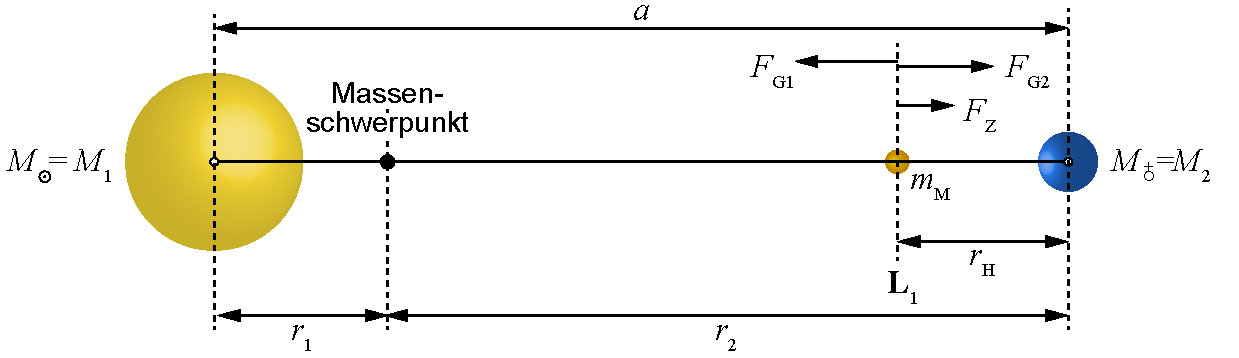
\includegraphics[width=0.8\textwidth]{Moon_of_Moon.pdf} 
	\caption[Zur Ableitung der Stabilit�tsbedingung.]{Zur Ableitung der Stabilit�tsbedingung (Hill Sph�re).}
	\label{abb:hm_Moon_of_Moon}
\end{figure}

Dann wollen wir uns einen ausgezeichneten Punkt zwischen den Massen $m_1$ und $m_2$ anschauen, an dem sich die Testmasse $m$ stabil aufhalten kann.
Dieser Punkt wird Lagrange-Punkt L$_1$ genannt.
Eine dort befindliche Testmasse $m$ rotiert um den Massenschwerpunkt des $m_1$-$m_2$-Systems mit der \emph{gleichen} Winkelgeschwindigkeit $\omega$ wie die Masse $m_2$.\footnote{Gewisserma�en \anf{geh�rt} die Testmasse an diesem Punkt weder zu $m_1$ noch zu $m_2$.
Es ist also der Grenzfall.} Wir erhalten aus der Geometrie der \figref{hm_Moon_of_Moon} die Abst�nde zum Massenschwerpunkt
\begin{align}
	r_1 &= \lk \frac{m_2}{m_1 + m_2} \rk a ~~\text{und} ~~~	r_2 = \lk \frac{m_1}{m_1 + m_2} \rk a ~.\label{eq:hm_moon_moon_lsg2}
\end{align}
Auf die Masse $m$ wirkt wegen ihrer kreisf�rmigen Bewegung um den Massenschwerpunkt die Zentrifugalkraft
\begin{equation}
F_z = m\omega^2 (r_2-r_\text{H}) ~~,\label{eq:hm_moon_moon_lsg3}
\end{equation}
worin wir $\omega$ durch das 3. Keplersche Gesetz ausdr�cken k�nnen:
\begin{equation}
\omega^2 = \frac{G(m_1+m_2)}{a^3}\label{eq:hm_moon_moon_lsg4} ~~.
\end{equation}
Es muss aber auch an dem Punkt L$_1$ die Zentrifugalkraft gleich den wirkenden Gravitationskr�ften der Massen $m_1$ und $m_2$ sein (damit ein Gleichgewicht herrscht), also
\begin{equation}
m\omega^2(r_2 - r_\text{H}) = \frac{Gmm_1}{(a-r_\text{H})^2} - \frac{Gmm_2}{r_\text{H}^2} ~~. \label{eq:hm_eq:moon_moon_lsg5}
\end{equation}
Wir setzen $\omega^2$ aus \eqref{eq:hm_moon_moon_lsg4} ein, dividieren durch $m$ und $G$ und erhalten
\begin{equation}
\frac{m_1+m_2}{a^3}(r_2-r_\text{H}) = \frac{m_1}{(a-r_\text{H})^2} - \frac{m_2}{r_\text{H}^2} ~~.\label{eq:hm_moon_moon_lsg6}
\end{equation}
Mit Substitution von $r_2$, $\gamma_\text{R}\!=\!m_2/m_1$ und $q\!=\!r_\text{H}/a$ erhalten wir aus \eqref{eq:hm_moon_moon_lsg6}
\begin{align}
	m_1 a- (m_1 + m_2) r_\text{H} &= \frac{m_1 a^3}{(a-r_\text{H})^2} - \frac{m_2 a^3}{r_\text{H}^2} ~~\Rightarrow~~a-(1+\gamma_\text{R})r_\text{H} = \frac{a^3}{(a-r_\text{H})^2} - \frac{\gamma_\text{R}a^3}{r_\text{H}^2} \nonumber\\
	\Rightarrow 1-(1+\gamma_\text{R})q &= \frac{1}{(1-q)^2} - \frac{\gamma_\text{R}}{q^2} ~~.\label{eq:hm_moon_moon_lsg7}
\end{align}
Diese Gleichung kann man nur numerisch l�sen, da sie ein Polynom 5. Grades in $q$ ist.
Umgeformt lautet sie
\begin{equation}
(1-q)^2 q^2 - (1+\gamma_\text{R})q^3 (1-q)^2 = q^2 - \gamma_\text{R}(1-q)^2 ~~.\label{eq:hm_moon_moon_lsg8}
\end{equation}
Wir k�nnen die Gleichung entweder numerisch l�sen und erhalten $q\!=\!r_\text{H}/a\!=\!f(\gamma_\text{R})$ (gute �bung in \matlab), oder wir machen eine sinnvolle N�herung, die z.\,B. f�r das Sonne-Erde-Mond-System gilt, mit 
\begin{align*}
	\gamma_\text{R} &= \frac{m_2}{m_1} \ll 1 ,\, q \ll 1 ~~~\Rightarrow 1+\gamma_\text{R} \approx 1 \;,~~(1-q)^2 \approx 1-2q \;~~\frac{1}{(1-q)^2} \approx= 1+2q ~~.
\end{align*}
Dann folgt aus \eqref{eq:hm_moon_moon_lsg7}
\begin{align*}
	1-q &= 1+2q - \frac{\gamma_\text{R}}{q^2} 	\Rightarrow q^2 - q^3 = q^2 + 2q^3 - \gamma_\text{R} ~~~	\Rightarrow ~~3q^3 = \gamma_\text{R} ~~
\end{align*}
und nach Resubstitution von $\gamma_\text{R}$ schlie�lich
\begin{equation}
r_\text{H} = a \sqrt[3]{\frac{m_2}{3 m_1}} ~~.\label{eq:hm_moon_moon_lsg9}
\end{equation}
Damit haben wir den maximalen Radius bestimmt, den ein Satellit mit Masse $m_2$ eines Planeten haben kann, bevor er vollst�ndig in das Gravitationsfeld des Zentralk�rpers mit Masse $m_1$ gelangt und selbst zum Kometen oder Planeten wird.
Dieser Radius wird zu Ehren von G. W. Hill\footnote{George William Hill (1838--1914) war ein US-amerikanischer Mathematiker und Astronom, der besonders auf dem Gebiet der theoretischen Astronomie zu Dreik�rperproblemen und der Mondtheorie forschte.} \emph{Hill-Radius} bzw. das entsprechende Volumen \emph{Hill-Sph�re} genannt.\\
Wir wollen zun�chst $r_\text{H}$ des Sonne-Erde-Mond-Systems berechnen.
Mit den Werten f�r $m_\text{\astrosun}\!=\!1.989\cdot 10^{30}\:$kg und $m_\text{\earth}\!=\!5.972\cdot 10^{24}\:$kg ergibt sich $r_\text{H,\earth}\!\approx\! 1.49\cdot 10^6\:$km.
Der Mond befindet sich mit einem Erdabstand von ca. $383000\:$km also gut innerhalb der Hill-Sph�re. \\
Wie sieht es nun aber beim Erde-Mond-\anf{Mond-Mond}-System aus?
Es folgt mit den Werten $m_\text{\earth}$ und $m_\text{M}\!=\!7.3\cdot 10^{22}\:$ kg ein Radius von $r_\text{H,M}\!\approx\! 61000\:$ km f�r die Hill-Sph�re.
Das ist etwas mehr als $1/7$ der Erde-Mond-Entfernung.
Es k�nnte also durchaus m�glich sein, dass der Mond selbst einen Begleiter hat (oder hatte).
Dass dies aber heute in der Realit�t nicht so ist, liegt an den starken Gezeitenkr�ften, die von Erde und Mond auf den Satelliten wirken und ihn mit der Zeit abbremsen w�rden (siehe \kap{adyn_forces}).
Nach einer gewissen Zeit in der Mondumlaufbahn w�rde die Testmasse (der Satellit) auf den Mond st�rzen. 
Es sei zum Schluss noch erw�hnt, dass die Formel f�r die Hill-Sph�re f�r elliptische Bahnen
\begin{equation}
r_\text{H} = (1-e)\,a\,\sqrt[3]{\frac{m_2}{3m_1}} \,. \label{eq:hm_hill_sphere_allg}
\end{equation}
lautet, was relativ einsichtig ist und im Detail in \cite{Murray2008} nachvollzogen werden kann.
\medskip \end{sol}
\textcolor{blue} {$\rightarrow$ zur} \probref{hm_hill_sphere}.\\
\noindent\rule[1ex]{\textwidth}{0.5pt} \newpage

%-----------------------------------------------------------------------------------------------------------

\begin{sol}{prob:hm_potential_merkur}\label{lsg:hm_potential_merkur} %�bung43
\textbf{Berechnung St�rpotential Merkur}\\
\begin{figure}[H]
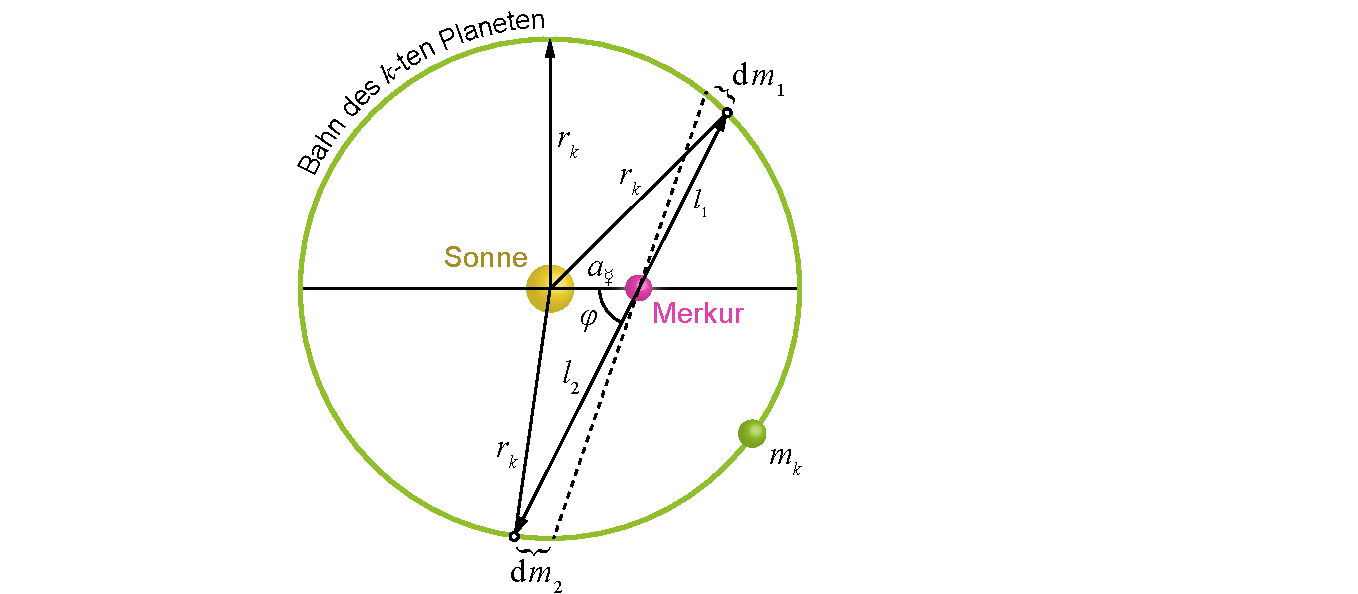
\includegraphics[width=\textwidth]{StoerpotentialMerkur_lsg}%
\caption[Geometrie zur Wirkung des St�rpotentials auf Merkur.]{Geometrie zur Wirkung des St�rpotentials einer Masse $m_k$ auf den Merkur.}%
\label{abb:hm_stoerpot_merkur_lsg}%
\end{figure}

Die Rechnungen sind im Detail im \mscr{} \mlhmref{StoerpotentialMerkur.m} ausgef�hrt. 
\begin{enumerate}[(a)]
	\item Wir benutzen die Geometrie der \figref{hm_stoerpot_merkur_lsg}.
          Der �u�ere Planet mit der Masse $m_k$ bewege sich gleichf�rmig auf der Kreisbahn mit $r_k$.
          Wir k�nnen dann seine Masse im Mittel \anf{verschmiert} auf den Ring mit dem Umfang $2\pi r_k$ verteilt annehmen.
          Die differentielle Massendichte auf der Umlaufbahn des $i$-ten Planeten mit dem Umfang $u_i$, die vom Merkur unter einem Winkel $\varphi$ gesehen wird, ist 
\begin{equation}
\D m_i = \lambda_k \,\D u_i = \frac{m_k}{2\pi r_k}\, l_i\,\D\varphi ~~. \label{eq:hm_pot_merk_lsg1}
\end{equation}
Die Newtonsche Gravitationskraft, die auf den Merkur wirkt, ist jeweils die Differenz der Massenwirkung $\D m_1$ und $\D m_2$, also
\begin{equation}
\D \vec{F} = m_\text{\mercury} G \lk \frac{\D m_1}{l_1^2} - \frac{\D m_2}{l_2^2} \rk \vec{l} ~~. \label{eq:hm_pot_merk_lsg2}
\end{equation}
Hierin ist $\vec{l}$ der Vektor, der vom Merkur zum differentiellen Massepunkt $\D m_1$ zeigt und, wie wir gleich sehen werden, eine Funktion des Winkels $\varphi$ ist.
Die Kraft, die in Richtung der Achse Sonne-Merkur wirkt (das ist die interessante Komponente, die ja das ZK-Feld der Sonne modifiziert), k�nnen wir schreiben als
\begin{equation*}
\D\vec{F}_{\text{SM}} = \D \vec{F}\,\cos\varphi ~~.
\end{equation*}
Wir k�nnen nun �ber $\D\vec{F}_{\text{SM}}$ integrieren und erhalten f�r den Beitrag des $k$-ten �u�eren Planeten �ber
\begin{equation*}
\D\vec{F}_{k,\text{SM}} = \vec{e}_{\text{\astrosun\mercury}}\,\int\limits_{-\pi/2}^{\pi/2} m_\text{\mercury} G \lambda_k \lk \frac{l_2 - l_1}{l_1 l_2} \rk \cos\varphi\,\D\varphi ~~.
\end{equation*}
Hierin haben wir mit $\vec{e}_{\text{\astrosun\mercury}}$ den Einheitsvektor in Richtung Sonne-Merkur bezeichnet.
Wir brauchen jetzt noch die $\varphi$-Abh�ngigkeit der L�ngen $l_1$ und $l_2$.
Mit dem Kosinussatz gilt
\begin{align*}
r_k^2 &= a^2 + l_1^2 - 2a l_1 \cos(\pi-\varphi) \\
\Rightarrow l_1 &= -a \cos\varphi + \sqrt{a^2\cos^2\varphi - \lk a^2-r_k^2 \rk}
\end{align*}
und
\begin{align*}
r_k^2 &= a^2 + l_2^2 - 2a l_2 \cos(\varphi) \\
\Rightarrow l_2 &= a \cos\varphi + \sqrt{a^2\cos^2\varphi - \lk a^2-r_k^2 \rk} ~~.
\end{align*}
Aus \eqref{eq:hm_pot_merk_lsg1} in \eqref{eq:hm_pot_merk_lsg2} eingesetzt erhalten wir
\begin{align*}
\D\vec{F}_{k,\text{SM}} &= m_\text{\mercury} G \lambda_k \lk \frac{l_1}{l_1^2} - \frac{l_2}{l_2^2} \rk \vec{l}\,\D\varphi \\
&= m_\text{\mercury} G \lambda_k \lk \frac{l_2 - l_1}{l_1 l_2} \rk \vec{l}\,\D\varphi ~~.
\end{align*}
Wir erkennen ferner aus der \figref{hm_stoerpot_merkur_lsg}, dass es zu den Kraftkomponenten, die senkrecht zu der Achse Sonne-Merkur wirken, jeweils eine positive und negative Komponente gibt.
Es verbleibt demnach als Netto-Effekt nur eine Komponente des Kraftvektors in Richtung Sonne-Merkur.
Wir machen weiter mit der hilfreichen Beziehung
\begin{align*}
\frac{l_2-l_1}{l_1 l_2} &= \frac{2a_\text{\mercury} \cos\varphi}{\killA{-a^2\cos^2\varphi} + \killA{a^2\cos^2\varphi} - (a^2_\text{\mercury} - r_k^2)} = \frac{2a_\text{\mercury} \cos\varphi}{r_k^2 - a_\text{\mercury}^2}
\end{align*}
und erhalten f�r die Gravitationskraft schlie�lich
\begin{align*}
F_k &= \frac{2 m_\text{\mercury} a_\text{\mercury} G}{r_k^2 - a_\text{\mercury}^2}\,\lambda_k \int\limits_{-\pi/2}^{\pi/2} \cos^2\varphi \, \D\varphi = \frac{\pi m_\text{\mercury} a_\text{\mercury} G \lambda_k}{r_k^2 - a_\text{\mercury}^2} ~~.         
\end{align*}
Die Wirkung des �u�eren Planeten ist also eine zentrale von der Sonne wegziehende Kraft (was nicht ganz �berraschend ist).
Grundlage f�r dieses Ergebnis waren folgende Annahmen:
\begin{itemize}
	\item Konzentrische Kreisbahnen der �u�eren Planeten und des Merkurs um die Sonne
	\item Wirkung des �u�eren Planeten auf den Merkur sind sehr klein
\end{itemize}

\item Wir berechnen die Frequenz $\omega\!=\!\sqrt{(-3/a) b(a)\!-\! b'(a)}\!\equiv\!\sqrt{\beta}$ nach \eqref{eq:hm_lsg_Stoer}.
  Stabile Bahnen gibt es, wenn der Ausdruck $\beta$ unter der Wurzel $>\!0$ ist.
  Wir berechnen die Beschleunigungen aus
\begin{align*}
b(r) &= -\frac{\d}{\d r}\,U(r) ~~\; \text{und} ~~\; b'(r) = -\frac{\d^2}{\d r^2}\,U(r) ~~.
\end{align*}
\begin{itemize}
	\item F�r den Fall $U(r)\!=\!-r^q$ ergibt sich 
	\begin{align*}
		b(r) &= +q r^q ~\;\text{und} ~\;	b'(r)= q(q-1)r^{q-1} ~~.
	\end{align*}
Mit $r\!=\!q\!=\!1$ folgt 
  \begin{align*}
		\beta &= -3q-q(q-1) > 0 ~~, \\
		\beta &= q(q+2) < 0 ~~.
	\end{align*}
Damit ist der stabile Bereich gegeben durch $-2\!<\!q\!<\!0$.
\smallskip
	\item F�r den Fall $U(r)\!=\! -1/r + C/r^3$ ergibt sich 
 	\begin{align*}
		b(r) &= -\frac{1}{r^2} + \frac{3C}{r^4} ~\;\text{und} ~\;	b'(r) = +\frac{2}{r^3} - \frac{12C}{r^5} ~~.
	\end{align*}
Mit $r\!=\!q\!=\!1$ folgt 
   \begin{align*}
		\beta &= -3(-1+3C)-2-12C >0 ~~, \\
		\beta &= 1+3C >0 ~~.
	\end{align*}
Damit ist der stabile Bereich gegeben durch $C\!>\! -1/3$.
\smallskip
\end{itemize}
\end{enumerate}
\medskip \end{sol}
\textcolor{blue} {$\rightarrow$ zur} \probref{hm_potential_merkur}.\\
\noindent\rule[1ex]{\textwidth}{0.5pt} \newpage


%-----------------------------------------------------------------------------------------------------------

\begin{sol}{prob:hm_perihel_kappa3}\label{lsg:hm_perihel_kappa3} %�bung44
\textbf{L�sung der Bewegungsgleichung und Periheldrehung bei einem $\kappa_3/r^3$ St�rpotential und Berechnung der relativistischen Perihelverschiebung des Merkurs}\\ \\
Wir setzen zun�chst in Gleichung \eqref{eq:hm_allg_ZK_1} $\kappa_2\!=\!0$.
Das ergibt
\begin{align}
\D \upsilon &= -\frac{\D q}{\sqrt{\frac{2H_g}{L^2} + \frac{2\mu_\text{G}}{L^2} q - \lk 1 - \frac{2\kappa_3 }{L^2} q \rk q^2 }} \nonumber \\
&= -\frac{\D q}{\sqrt{\hat{A}+ \hat{B} q + \hat{C} q^2 + \hat{D} q^3 }} ~~, \label{eq:hm_perihel_lsg_1} 
\end{align}
mit den Abk�rzungen
\begin{align*}
	\hat{A} = \frac{2H}{L^2} < 0 ~, \: \hat{B} = \frac{2\mu_\text{G}}{L^2} > 0 ~,\:	\hat{C} = -1 < 0 ~\; \text{und} ~\;\hat{D} = \frac{2\kappa_3}{L^2}~~.
\end{align*}
Dieses Integral ist nicht analytisch l�sbar.
Allenfalls kann man eine Reihenentwicklung machen.
Wir verfolgen hier einen st�rungstheoretischen Ansatz \cite{Greiner2003, Stephani1991}.
Dazu schreiben wir wieder die Radialbeschleunigung \eqref{eq:hm_beschl_polar} in Polarkoordinaten:
\begin{equation}
b(r) = b \lk \frac{1}{q} \rk = \lk \ddot{r} - r\dot{\upsilon}^2 \rk = -\frac{\d}{\d r}U(r) ~~.\label{eq:hm_perihel_lsg_2}
\end{equation}
F�r $\dot{r}$ gilt:
\begin{equation*}
\dot{r} = \frac{\D r}{\D \upsilon}\,\dot{\upsilon} = -\frac{1}{\killA{q^2}} \frac{\D q}{\D \upsilon} L \killA{q^2} = -L\,\frac{\D q}{\D \upsilon}~~
\end{equation*}
und analog f�r $\ddot{r}$: 
\begin{align*}
	\ddot{r} = \frac{\D}{\D t}\dot{r} &= -L \, \frac{\D}{\D t} \lk \frac{\D q}{\D \upsilon} \rk = -L \frac{\D }{\D \upsilon}\frac{\D \upsilon}{\D t} \lk \frac{\D q}{\D \upsilon} \rk = -L^2 q^2\,\frac{\D^2 q}{\D \upsilon^2}~~.
\end{align*}
Wir setzen beide Beziehungen in \eqref{eq:hm_perihel_lsg_2} ein und bekommen
\begin{align}
	-L^2 q^2 \,\frac{\D^2 q}{\D \upsilon^2} - \frac{1}{q}\,L^2 q^4 &= -\frac{\d}{\d r}U(r) = -\frac{\mu_\text{G}}{r^2} + \frac{3\kappa_3}{r^4}\nonumber\\
\Rightarrow \frac{\D^2 q}{\D \upsilon^2} + q &= \frac{1}{L^2 q^2}\,\frac{\d}{\d r}U(r) ~\nonumber\\
&= \frac{\mu_\text{G}}{L^2} - \frac{3\kappa_3}{L^2} q^2 ~. \label{eq:hm_perihel_lsg_3} 
 \end{align}
F�r $\kappa_3\!=\!0$ ergibt sich die bemerkenswert einfache Differentialgleichung 
\begin{equation}
\frac{\D^2 q}{\D \upsilon^2} + q = \frac{\mu_\text{G}}{L^2} \label{eq:hm_perihel_lsg_4} ~~, 
\end{equation}
aus deren L�sung sich sehr einfach die Bahnform bestimmen l�sst.
Denn es ist 
\begin{equation}
q(\upsilon) = \frac{\mu_\text{G}}{L^2} + A \cos\upsilon+ B\sin\upsilon \label{eq:hm_perihel_lsg_5} ~~,
\end{equation}
woraus man mit $q\!=\!1/r$ und $A\cos\upsilon + B\sin\upsilon\!=\! C\cos(\upsilon-\upsilon_0)$ nicht �berraschend die bekannte Kegelschnittgleichung \eqref{eq:hm_kegelschnitt} des Keplerproblems erh�lt.\footnote{Ohne Beschr�nkung der Allgemeinheit kann man $\upsilon_0\!=\!0$ setzen.} Wir erweitern nun \eqref{eq:hm_perihel_lsg_5} um $-3\kappa_3 q^2$ und schreiben f�r $\D^2 q / \D \upsilon^2 \!=\! q''$, so dass aus \eqref{eq:hm_perihel_lsg_3} folgt
\begin{align}
	q'' + q &= \frac{\mu_\text{G}}{L^2} - \frac{3\kappa_3 q^2}{L^2} \label{eq:hm_perihel_lsg_6}\\
	&\equiv A + \frac{B}{A}\,q^2 ~~, \nonumber
\end{align}
wobei $A\!=\!\mu_\text{G}/L^2 = 1/p$, $B/A\!=\!-3\kappa_3/L^2$ und $B\!=\!-3\kappa_3\mu_\text{G}/L^4$ gesetzt wurde.
Da $\kappa_3$ und daher $B/A$ kleine Gr��en sind, k�nnen wir f�r die L�sung dieser inhomogenen Differentialgleichung folgenden Ansatz machen:
\begin{align}
q &\approx q_K + B\:\hat{q} ~\label{eq:hm_perihel_lsg_7}\\
\Rightarrow q''_K + q_K + B \hat{q}'' + B\hat{q} &= A + \frac{B}{A} \lk q^2_K + 2 B\! q_K \!\hat{q} + B^2 \hat{q}^2 \rk ~~,
\end{align}
worin $q_K$ die Keplerl�sung f�r $\kappa_3\!=\!0$ ist.
Wir sortieren nach Potenzen von $B$ und bis zur Ordnung mit $B^1$.
Damit ergibt sich
\begin{align}
B^0 : ~ &q''_K + q_K = A ~~. \label{eq:hm_perihel_lsg_8a} \\ 
B^1 : ~ &\hat{q}'' + \hat{q} = \frac{1}{A} \lk q_K^2 + 2B \!q_K \hat{q}\rk = \frac{q_K}{A} \lk q_K + 2\hat{q} B \rk ~~\Rightarrow ~~\hat{q}'' + \hat{q} \lk 1 - \frac{2 B q_K}{A} \rk \approx \frac{q_K^2}{A}~~.  \label{eq:hm_perihel_lsg_8b}
\end{align}
Gleichung \eqref{eq:hm_perihel_lsg_8a} ist wie erwartet die bekannte Kepler-L�sung.
Wir setzen jetzt in \eqref{eq:hm_perihel_lsg_8b} f�r $q_K$ die Bahngleichung in der Form \eqref{eq:hm_kegelschnitt} ein und erhalten mit $q_K(\upsilon) = 1/p (1 + e\cos\upsilon) = A (1 + e\cos\upsilon) $ und $(A=1/p)$
\begin{align*}
	\hat{q}'' + \hat{q} &= p \lek \frac{1}{p} \lk 1+e\cos\upsilon\rk\rek^2 = \frac{1}{p} \lk  1+2e\cos\upsilon + \underbrace{e^2\cos^2\upsilon}_{= \frac{e^2}{2}(1+\cos 2\upsilon)}\rk \\
											&= \frac{1}{p} \lk  1+\frac{e^2}{2}+ 2e\cos\upsilon + \frac{e^2}{2}\cos 2\upsilon \rk~~.
\end{align*}
Da wir an Irregularit�ten der Bahn interessiert sind, schreiben wir die gesuchte Gesamtl�sung als lineare Superposition  $\hat{q}\!=\!\hat{q}_1 + \hat{q}_2 + \hat{q}_3$ und sortieren die einzelnen Elemente nach Vielfachen von $\upsilon$ im Argument des Kosinus:  
\begin{align}
\begin{split}
	\cos(0\upsilon): ~~ \hat{q}''_1 + \hat{q}_1 &= \frac{1}{p} \lk 1+\frac{e^2}{2}\rk~~, \\
	\cos(1\upsilon): ~~ \hat{q}''_2 + \hat{q}_2 &= 2\frac{e}{p} \cos\upsilon ~~, \\
	\cos(2\upsilon): ~~ \hat{q}''_3 + \hat{q}_3 &= \frac{e^2}{2p} \cos 2\upsilon ~~.
\end{split} \label{eq:hm_perihel_lsg_09a}
\end{align}
Die Einzell�sungen $\hat{q}_i$ der linearen Superposition sind (wie man leicht durch Differenzieren verifiziert):
\begin{align}
\begin{split}
\hat{q}_1 &= \frac{1}{p} \lk 1+\frac{e^2}{2}\rk ~~, \\
\hat{q}_2 &= \frac{e}{p}\,\upsilon \sin\upsilon ~~,\\ 
\hat{q}_3 &= -\frac{e^2}{6p}\,\cos 2\upsilon ~~.
\end{split} \label{eq:hm_perihel_lsg_09b}
\end{align}
Der eigentlich interessante Term ist der f�r $\hat{q}_2$.
Man erkennt an dieser Stelle, dass die Periheldrehung durch den nichtlinearen St�ranteil, der in der \eqref{eq:hm_perihel_lsg_3} vorhanden ist, hervorgerufen wird.
Die Gleichung f�r die gest�rte Bahn k�nnen wir schreiben als Keplerbahn plus St�rung $\hat{q}$:
\begin{equation}
q(\upsilon) = q_K + B \hat{q} = \frac{1+e\cos\upsilon}{p} + B (\hat{q}_1 + \hat{q}_2 + \hat{q}_3)~~. \label{eq:hm_perihel_lsg_9}
\end{equation}
Wir wollen jetzt analysieren, wie diese einzelnen St�rungen wirken.
Dazu fahren wir fort mit
\begin{equation}
pq(\upsilon) = 1 + \underbrace{e\cos\upsilon + Be\upsilon\sin\upsilon}_{\text{Term P}} + 1 + B \lek \lk 1+\frac{e^2}{2}\rk - \frac{e^2}{6} \cos{2\upsilon} \rek ~~, \label{eq:hm_perihel_lsg_10}
\end{equation}
wobei nur Term P zur Modifikation der Keplerbahn in Form einer Perihelverschiebung beitragen kann.
Wir k�nnen jetzt mit den Winkelfunktionen und unter Beachtung von $B \ll 1$ folgende Beziehung nutzen:
\begin{align*}
e\cos(\upsilon-B\upsilon)	&= e\cos\upsilon\,\underbrace{\cos(B\upsilon)}_{\approx 1} + e\sin\upsilon\,\underbrace{\sin(B\upsilon)}_{B\upsilon} = e\cos\upsilon + (Be\upsilon)\,\sin\upsilon\,
\end{align*}
Damit vereinfacht sich \eqref{eq:hm_perihel_lsg_10} zu
\begin{align*}
p\,q(\upsilon) &= 1 + \underbrace{e\cos(\upsilon-B\upsilon)}_{\text{Term I}} + B \underbrace{\lk a+\frac{e^2}{2} - \frac{e^2}{6}\,\cos 2\upsilon\rk}_{\text{Term II}}~~,
\end{align*}
wobei Term I \emph{nicht-periodisch} in $2\pi$ ist (und damit zu einer Periheldrehung f�hrt) w�hrend Term II periodisch in $2\pi$ (und damit nur f�r eine Oszillation des Radius verantwortlich ist).
Wir erhalten schlie�lich 
\begin{align}
r(\upsilon)	 &= \frac{p}{1+e\cos(\upsilon-B\upsilon)} \lk 1+ \frac{B C p}{1+e\cos{(\upsilon-B\upsilon)}} \rk^{-1} ~~. \label{eq:hm_perihel_lsg_11}
\end{align}
Damit haben wir eine n�herungsweise Beschreibung der Bahn f�r den gest�rten Fall mit $\kappa_3 \neq 0$ gewonnen.
\begin{figure}[H]
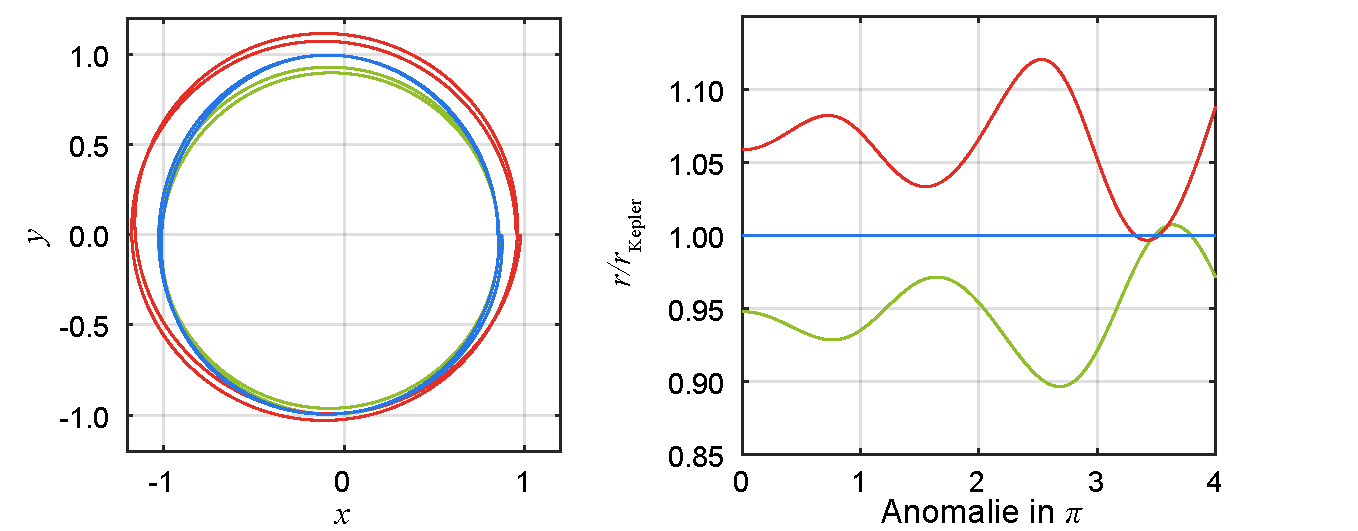
\includegraphics[width=\textwidth]{simulation_merkur2.pdf}%
\caption[Bahnkurven und Bahn-Oszillationen im Fall eines St�rpotentials.]{Bahnkurven und Bahn-Oszillationen im Fall eines St�rpotentials mit $\kappa_3 /{r^3}$\\ Parameter: $a=1, e = 0.1, \kappa_3 = + 0.02\,\mu_\text{G}/a^2 >0 $ (rot) und $\kappa_3-0.02\,\mu_\text{G}/a^2 < 0$ (gr�n). In blauer Farbe ist die Keplerl�sung dargestellt (\scref{prob:hm_perihel_kappa3}).}%
\label{abb:hm_simulationen_merkur2}%
\end{figure} 

F�r $\kappa_3$ k�nnen wir z.\,B. auch das relativistische Zusatzpotential \eqref{eq:hm_einstein_01} einsetzen.
In \figref{hm_simulationen_merkur2} sind im linken Bild die Bahnkurven f�r den Keplerfall (blau) als auch f�r die St�rpotentiale $\kappa_3 = + 0.02 \: \mu_\text{G}/a^2 > 0 $ (rot) und $\kappa_3-0.02 \: \mu_\text{G}/a^2 < 0$ (gr�n) dargestellt.
Im rechten Bild ist der Bahnradius �ber die Anomalie aufgetragen.
Die Bahnoszillationen sind deutlich zu erkennen.\\
Um die Periheldrehung und Verschiebungsrate f�r den Merkur zu erhalten, k�nnen wir mit $\upsilon_{\text{P}_0} (1-B) = 2 \pi $ fortfahren und schreiben:
\begin{align}
		\Delta \upsilon_{\text{P}_0} &= \upsilon_{\text{P}_0} - 2\pi \approx 2\pi \lk (1+B) - 1\rk  ~\: \text{bzw.} \nonumber \\
	\Delta \dot{\upsilon}_{\text{P}_0} &\approx \frac{2\pi B}{T_{\mercury}} = -2\pi\,\frac{3\kappa_3\mu_\text{G}}{T_{\mercury} \, L^4}
~~ \text{mit} ~ B = -\frac{3\kappa_3\mu_\text{G}}{L^4}~. \label{eq:hm_perihel_lsg_12}
\end{align}
Das hei�t, dass die Periheldrehung im Falle $\Delta U_3 \propto 1/r^3$ wie erwartet vom Drehimpuls und der St�rke der St�rung $\kappa_3$ abh�ngt.
F�r ein negatives $\kappa_3$, d.\,h.\, einem zus�tzlich anziehenden Potential, wie es z.\,B. im Fall des relativistischen Beitrags \eqref{eq:hm_einstein_01} vorliegt, ergibt sich ein Voranschreiten des Perihels ($\Delta \dot{\upsilon}_{\text{P}_0} > 0$) in �bereinstimmung mit unseren Absch�tzungen in \eqref{eq:hm_upsilon_P0}.
Setzen wir die Werte von \eqref{eq:hm_einstein_01} ein, erhalten wir mit den Gr��en 
\begin{align*}
\kappa_3 = - \frac{\mu_{\text{G}} L^2}{c^2} ~ \text{und} ~ L^2 \:=\: a \:\mu_{\text{G}} (1-e^2) 
\end{align*}
eine Verschiebungsrate von
\begin{align*}
\Delta \dot{\upsilon}_{\text{P}_0} = \frac{6 \pi}{c^2} \frac{\mu_{\text{G}}}{a(1-e^2)} \frac{1}{T_{\mercury}} \approx 43''/\text{Jh.}.
\end{align*}
Wir sehen, dass unsere Absch�tzung in \eqref{eq:hm_rel_perihel_val} f�r nahezu kreisf�rmige Bahnen in Kapitel \ref{kap:Stabile_Bahnen} sehr gut war.
Unsere st�rungstheoretische L�sung ber�cksichtigt auch noch die Elliptizit�t der Bahn, welche zu einem $4\,\% $ gr��eren Wert der Perihelverschiebung f�hrt.\\

F�r interessierte Leser sei auf eine sch�ne einfache, da linearisierte, Merkurpr�zessionsberechnung f�r den relativistischen Fall in \cite{Hall2022} verwiesen, die ebenfalls f�r ein nichtrelativistisches $\kappa_3/r^3$ St�rpotential verwendet werden kann.\\
\medskip \end{sol}
\textcolor{blue} {$\rightarrow$ zur} \probref{hm_perihel_kappa3}.\\
\noindent\rule[1ex]{\textwidth}{0.5pt} \newpage

%-----------------------------------------------------------------------------------------------------------

\begin{sol}{prob:hm_MoFi}\label{lsg:hm_MoFi} %�bung45
\textbf{Mond- und Sonnenfinsternisse}\\ \\
Aus den �berlegungen von Kapitel \ref{kap:basics_sofis} ist relativ klar, dass eine totale Mondfinsternis sehr h�ufig vor oder nach einer totalen Sonnenfinsternis auftreten muss.
Wir haben die Tage, an welchen im Zeitraum von 1990 bis 2040 m�gliche Sonnenfinsternisse (unabh�ngig vom Ort auf der Erde) und Mondfinsternisse aufgetreten sind \bzw noch auftreten werden, im Detail in \mlhmref{Sonnenfinsternis01.m} ausgef�hrt.
Aus den Rechnungen sieht man, dass am 07.\ August 2017 (18:13:01 UT), also ziemlich genau 14 Tage vor der Sonnenfinsternis vom 21.\ August 2017 (um 18:28.44 UT) eine partielle Mondfinsternis auftrat.
Diese war aber wegen der Uhrzeit und der Position des Mondes in Europa nur in der Endphase zu beobachten.\footnote{Um die Zeiten der Verfinsterung auf eine Sekunde genau berechnen zu k�nnen, braucht man Genauigkeiten in der Ephemeridenrechnung von etwa einer Bogensekunde.
Die in den \mscren verwendeten Funktionen \mlhmiref{SonneExakt.m} und \mlhmiref{MondExakt.m} wurden auf Basis von Daten aus \cite{Montenbruck1999, Meeus1998} geschrieben und haben Genauigkeiten von besser als 5 Bogensekunden.} Aus den Abbildungen erkennt man sehr sch�n das Auftreten von Zyklen der Finsternisse, die bereits im Altertum bekannt waren.
Der bekannteste ist der Saroszyklus\index{Saroszyklus}, der dadurch gekennzeichnet ist, dass seine Periode etwa 18.03 Jahre betr�gt und zwei seiner direkt folgenden Finsternisse sich sehr �hneln.
Das liegt daran, dass nach einer ganzen Zahl anomalistischer Monate der Mond sich wieder an demselben Ort auf seiner elliptischen Bahn um die Erde befindet.
Weil die Sarosperiode nur etwa 11 Tage l�nger als 18 ganze Jahre ist, befindet sich auch die Erde ann�hernd wieder am selben Ort der Erdbahn.
Aus diesem Grund wirft der Mond ann�hernd wieder den gleichen Schatten auf die Erde.

\begin{figure}[H]
\begin{minipage}{\textwidth}
\leftfigure{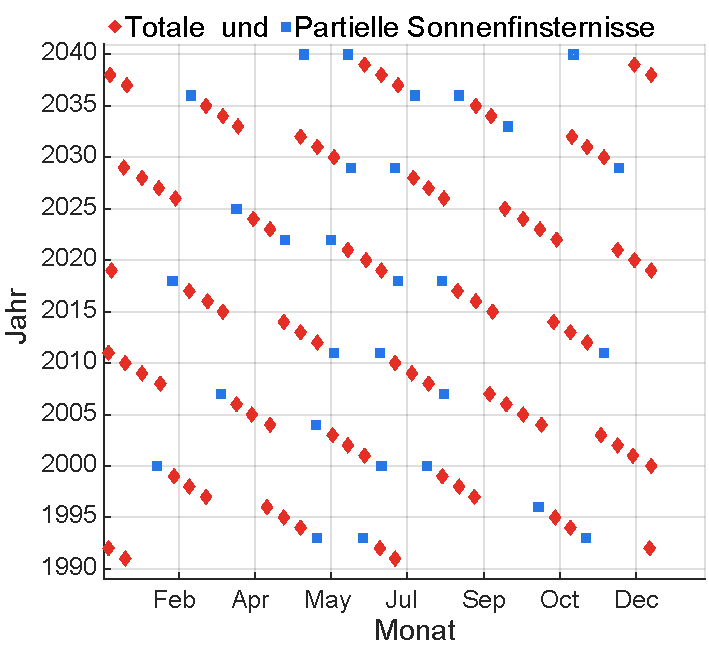
\includegraphics[width=0.5\textwidth]{Sonnenfinsternisse.pdf}}
\hspace{\fill}
\rightfigure{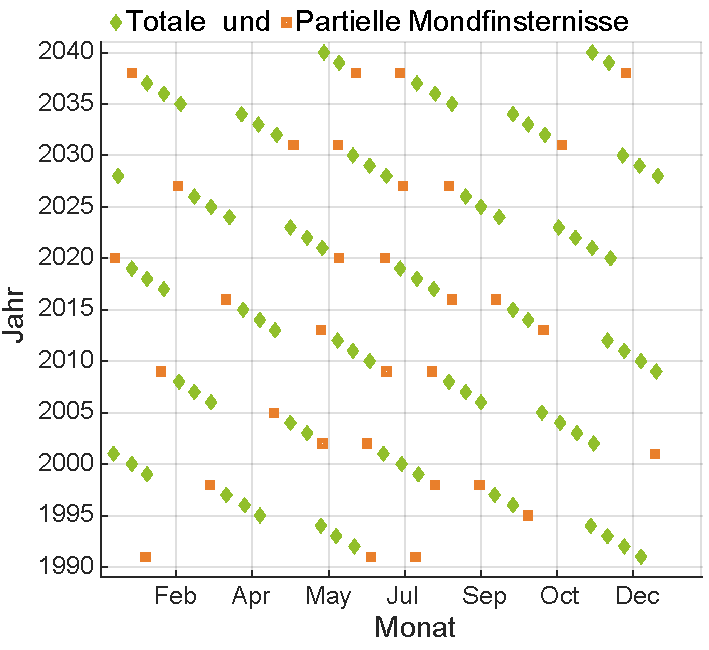
\includegraphics[width=0.5\textwidth]{Mondfinsternisse.pdf}}
\leftcaption[Sonnenfinsternisse 1990--2040.]{Sonnenfinsternisse 1990--2040}\label{abb:hm_Sonnenfinsternisse}
\rightcaption[Mondfinsternisse 1990--2040.]{Mondfinsternisse 1990--2040}\label{abb:hm_Mondfinsternisse}
\end{minipage}
\end{figure}

\medskip \end{sol}
\textcolor{blue} {$\rightarrow$ zur} \probref{hm_MoFi}.\\
\noindent\rule[1ex]{\textwidth}{0.5pt} \newpage

%-----------------------------------------------------------------------------------------------------------



%\clearpage
%\section{L�sungsbeispiele \autoref{chap:adyn} -- Astrodynamik}\label{chap:adyn_lsguebungen}

Die in den L�sungsvorschl�gen angegebenen \mscre finden sich im GitHub unter \githubSN \bzw
in den \onlineZ{} (\MKc).\\
Sie sind wirklich als Vorschlag f�r eine m�gliche L�sung gedacht, wohl wissend, dass es in der Physik oft ganz verschiedene, manchmal auch elegantere als die hier vorgestellten L�sungen gibt, um ein Problem zu l�sen. Das macht ja gerade den Reiz der Physik aus.
Wir laden die Leser ein, ihre L�sungen auch unter \githubSN \bzw auf den online-Seiten (\MKc) zu teilen.
Wir sind in jedem Fall gespannt.

%%-----------------------------------------------------------------------------------------------------------

\subsection{�bungen zu Grundlagen der Raketenphysik}

\medskip

-----------------------------------------------------------------------------------------------------------

\begin{sol}{prob:adyn_canonball}\label{lsg:adyn_canonball} %�bung1
\textbf{Jules Vernes Kanonenschuss zum Mond}\\

Wir wissen, dass ein Objekt, das zum Mond fliegen soll, eine bestimmte kinetische Energie braucht, um das Gravitationsfeld der Erde zu verlassen:
\begin{align*}
    \frac{m}{2}\,v^2 = G\,\frac{m_\text{E}\,m}{R_\text{E}}\,,
\end{align*}
woraus die 2.\,\gls{vkosmos} oder auch \gls{vescape} 
$v_\text{F} = \sqrt{2\,G\,m_\text{E}/R_\text{E}} \approx \SI{11.2}{\km\per\second}$
folgt. Das \textit{Problem Nr. 1} ist das Erreichen dieser Fluchtgeschwindigkeit. Im Buch gibt Verne eine Masse der Kapsel von \ca $m_\text{R} = \SI{8.75}{\tonne}$ und eine Sprengstoffmasse von Schie�baumwolle $m_\text{SB}$ von \ca $\SI{182}{\tonne}$ an. Schie�baumwolle (auch Nitrozellulose genannt) wurde 1846 entdeckt und hat eine f�r das Projekt \textit{Columbiade} relevante Detonationsgeschwindigkeit von $\SI{6300}{\metre\per\second}$ \bzw eine spezifische Explosionsenergie von $\epsilon = \SI{5475}{\kilo\J\per\kg}$.
Wir k�nnen den Energieerhaltungssatz aufschreiben und nehmen an, dass das Gas und die Kapsel an der Kanonenrohr�ffnung beim Verlassen dieser die gleiche Geschwindigkeit haben:
\begin{align*}
    \epsilon\,m_\text{SB}\,&= \frac{m_\text{SB}}{2}\,v^2 + \frac{m_\text{R}}{2}\,v^2  ~~~~ \rightarrow ~~~ v = \sqrt{\frac{2\,m_\text{SB}\,\epsilon}{m_\text{SB}+m_\text{R}}} = \SI{3232}{\metre\per\second}\,.
\end{align*}
Das ist deutlich geringer als die notwendigen $v_\text{F} = \SI{11.2}{\km\per\second}$. 
Das \textit{Problem Nr. 2} ist aber noch ein anderes: Selbst wenn es einen Sprengstoff g�be, der eine Geschwindigkeit von gr��er $\SI{11.2}{\km\per\second}$ an der Rohrm�ndung erlauben w�rde, m�sste auf der L�nge des Rohrs (nach Verne $s = \SI{270}{\metre}$) eine Beschleunigung von
\begin{align*}
    a = \frac{v_\text{F}{}^2}{2s} \approx \SI{2.32e5}{\metre\per\square\second} \approx \SI{23700}{}\, g
\end{align*}
wirken. Wenn man wei�, dass man bereits bei einer Belastung von $\SI{10}{}\,g$ in Ohnmacht fallen kann, wird es nicht viele Freiwillige gegeben haben. \\
Man k�nnte nat�rlich die Beschleunigungsstrecke l�nger machen, so dass nur $\SI{10}{}\,g$ auf die Astronauten wirken. Dann m�sste das Kanonenrohr aber 
$s = v_\text{F}{}^2/(\SI{20}{}\,g) \approx \SI{640}{\km}$ lang sein. %was l�nger ist als die Strecken M�nchen-Hamburg (612\,km) bzw. Baltimore-Boston (578 km).\\
\end{sol} 
\textcolor{blue} {$\rightarrow$ zur} \probref{adyn_canonball}.\\
\noindent\rule[1ex]{\textwidth}{0.5pt}  \newpage  \clearpage

%-----------------------------------------------------------------------------------------------------------

\begin{sol}{prob:adyn_rocketbasic}\label{lsg:adyn_rocketbasic} %�bung2
\textbf{Prinzip Mehrstufenrakete}\\ \\
Wir starten von \eqref{eq:adyn_rockets19} und zeigen zun�chst, dass f�r eine einstufige Rakete diese Gleichung in die Ziolkowski-Gleichung �bergeht ($N=i=1$)
\begin{align*}
    \Delta v_\text{ges} = v_\text{G}\,\ln\,\frac{m_1}{\sigma_1\,m_1+m_\text{L}} = v_\text{G}\,\ln\,\frac{1}{\sigma_1 + m_\text{L}/m_1}\,.
\end{align*}
Mit $\sigma_1\approx 0$ folgt daraus die Ziolkowski-Gleichung $\Delta v = v_\text{G}\,\ln(m_1/m_\text{L})$.\\
Wir setzen nun in \eqref{eq:adyn_rockets19} alle $v_{\text{G},i}= v_\text{G}{}^*$ und benutzen ebenfalls:
	\[\mathcal{M}^* = \frac{m_{0,i}}{m_{0,i}-m_{\text{T},i}}\,.	\]
\begin{align*}
    \Delta v = v_\text{G}^*\,\sum\limits_{i=1}^N\ln\,\frac{m_{0,i}}{\sigma_i\,m_{0,i} + m_{0,i+1}}\,.
\end{align*}
Nun war ja $\sigma_i$ definiert als \eqref{eq:adyn_rockets18}:
\begin{align*}
    \sigma_i = \frac{m_{0,i}- m_{\text{T},i}- m_{0,i+1}}{m_{0,i}}\,,
\end{align*}
womit wir erhalten:
\begin{align}
    \Delta v &= v_\text{G}^* \,\sum_{i=1}^N\ln\,\frac{m_{0,i}}{m_{0,i} - m_{\text{T},i} - \killA{m_{0,i+1}} + \killA{m_{0,i+1}}}\nonumber \\
             &= v_\text{G}^* \,\sum_{i=1}^N\ln\,\frac{m_{0,i}}{m_{0,i} - m_{\text{T},i} } =  v_\text{G}^* \,\sum_{i=1}^N\ln\,\mathcal{M}^* =  v_\text{G}^* \,N\,\ln \,\mathcal{M}^*\,. 
						\label{eq:adyn_lsg_rocket01}
\end{align}
Damit haben wir die erste Gleichung von \eqref{eq:adyn_rockets20} bewiesen. \\
Das Nutzlastverh�ltnis ist gegeben durch:
\begin{align*}
    \mu_\text{L}= \frac{m_\text{L}}{m_0} = \frac{m_\text{L}}{\sum\limits_{i=1}^N m_i+m_\text{L}}\,.
\end{align*}
Die Strukturmassen wollen wir gegen�ber den Treibstoffmassen vernachl�ssigen, so dass mit $\lk\mathcal{M}^*\rk^N$ und mit der Masse der $i$-ten Unterrakete
	\[ 
	m_{0,i} = \lk \sum\limits_{j=i}^N m_{\text{T},j} \rk + m_\text{L}  \approx m_{0,i-1} + m_{\text{T},i} 
	\]
(siehe auch \figref{adyn_rockets04}a gilt:
\begin{align*}
     \lk \mathcal{M}^* \rk ^N  &= \lk \frac{m_{0,i}}{m_{0,i}-m_{\text{T},i}}\rk^N \approx \frac{m_0}{ \lk \sum\limits_{i=2}^N m_{\text{T},i} \rk + m_\text{L}}\, \dot\,\frac{ \lk \sum\limits_{i=2}^N m_{\text{T},i} \rk + m_\text{L}}{\lk \sum\limits_{i=3}^N m_{\text{T},i} \rk + m_\text{L}}\,\dot\,\ldots \,\dot\, \frac{\lk \sum\limits_{i=N-1}^N m_{\text{T},i} \rk + m_\text{L}}{m_\text{L}}\,\approx\, \frac{m_0}{m_\text{L}}\,,
\end{align*}
woraus die zweite Gleichung von \eqref{eq:adyn_rockets20} 
\begin{align}
    \frac{m_\text{L}}{m_0} \approx \lk \mathcal{M}^*\rk^{-N}\, \label{eq:adyn_lsg_rocket02}
\end{align}
folgt.

\begin{figure}[H]
	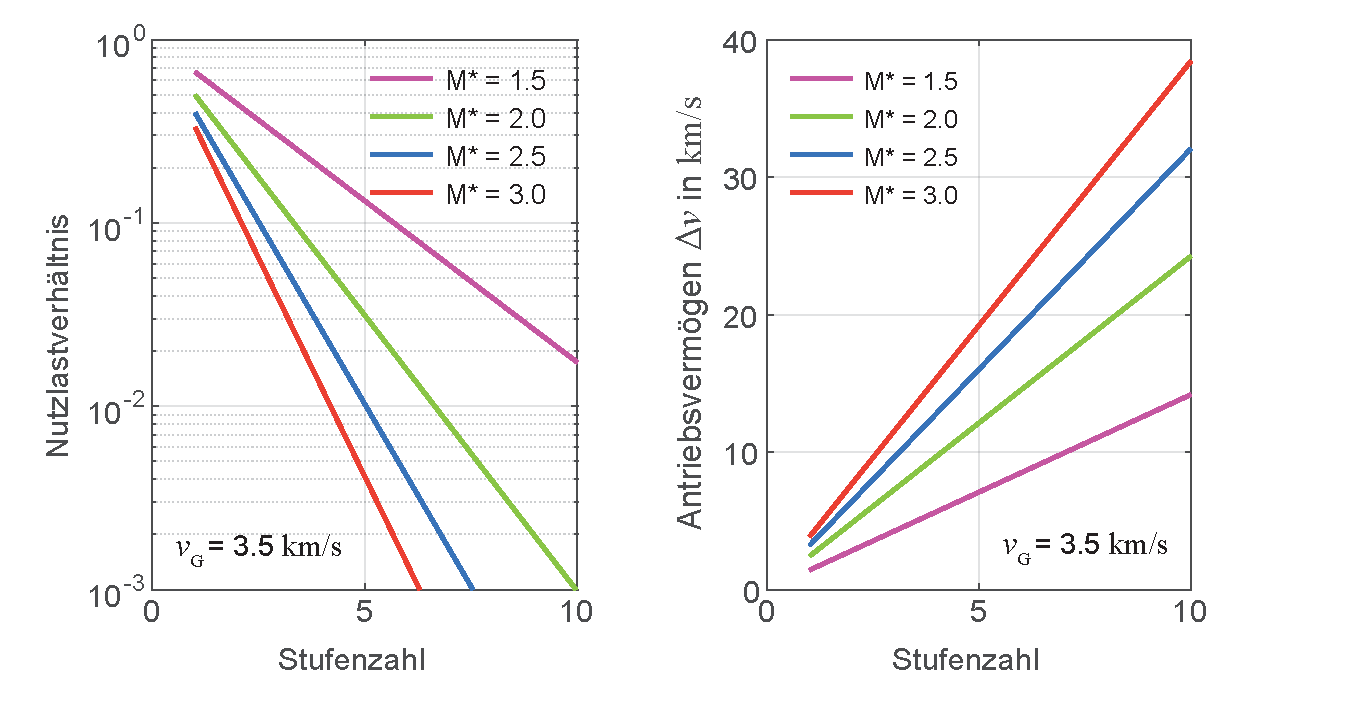
\includegraphics[width=\textwidth]{MehrStufenTheorie.pdf} 
	\caption[Nutzlastverh�ltnis �ber Antriebsbudget f�r mehrstufige Raketen.]{Nutzlastverh�ltnis �ber Antriebsbudget f�r mehrstufige Raketen bei gleichen $v_{\text{G},i}= v_\text{G}{}^*$ und 
	gleichen Struktur- und Treibstoffmassen aller Unterraketen ($\mathcal{M}^* = m_{0,i}/(m_{0,i}-m_{\text{T},i})$). Siehe \matlab{}-Datei
\mladynref{Raketenstart04.m}.}
	\label{abb:adyn_rocket_lsg05}
\end{figure}

\end{sol} 
\textcolor{blue} {$\rightarrow$ zur} \probref{adyn_rocketbasic}.\\
\noindent\rule[1ex]{\textwidth}{0.5pt}  \newpage  \clearpage

%-----------------------------------------------------------------------------------------------------------


\begin{sol}{prob:adyn_rocketopt1}\label{lsg:adyn_rocketopt1} %�bung3
\textbf{Optimierung Mehrstufenrakete (Tandemstufung)}\\
\begin{enumerate}
	\item \textit{\textbf{L�sungsansatz �ber Extremwertberechnung - Beispiel Saturn V Maximalleistung 100 t Nutzlast}}\\ 
Wir starten von der Raketen-Gleichung f�r die Tandemstufung \eqref{eq:adyn_rockets19} und fordern, dass f�r ein Nutzlastverh�ltnis
\begin{align}
    \Delta v = \sum\limits_{i_1}^N \Delta v_i = \sum\limits_{i_1}^N v_{\text{G},i}\,\ln\,\frac{1}{\sigma_i + \frac{\mu_{i+1}}{\mu_i}}\,.\label{eq:adyn_rocketsopt01} ~~~~ \rightarrow ~~~~ \text{max}
\end{align}
gelten soll. Die Bedingung f�r das Maximum lautet, wenn $\mu_\text{L}$ und alle $\sigma_i$ gegeben sind:
\begin{align}
    \frac{\d \Delta v\lk\mu_2,\mu_3,\ldots,\mu_N\rk}{\d \mu_i} = 0 ~~~~ \text{f�r} ~~~~i= 2,3,\ldots,N\,.\label{eq:adyn_rocketsopt02}
\end{align}
Daraus folgt sofort:
\begin{align}
    \frac{\d}{\d\mu_i}\,\lek -v_{\text{G},i-1}\,\ln\lk\sigma_{i-1} + \frac{\mu_i}{\mu_{i-1}}\rk- v_{\text{G},i}\,\lk\sigma_i + \frac{\mu_{i+1}}{\mu_i}\rk\rek= 0\,.\label{eq:adyn_rocketsopt03}
\end{align}
Wir f�hren  die Ableitung aus und erhalten $N-1$ Gleichungen in $\mu_i$ der Form: ($i=2,3,\ldots,N$)
\begin{align}
    \mu_i{}^2 = \frac{\lk v_{\text{G},i}-v_{\text{G},i-1}\rk\,\mu_{i+1}}{v_{\text{G},i-1}\,\sigma_i}\,\mu_i-\frac{v_{\text{G},i}}{v_{\text{G},i-1}}\,\frac{\sigma_{i-1}}{\sigma_i}\,\mu_{i-1}\,\mu_{i+1} = 0 \,,\label{eq:adyn_rocketsopt04}
\end{align}
\bzw aufgel�st nach
\begin{align}
    \mu_i = Q_i\,\mu_{i+1}+\sqrt{\lk Q_i\,\mu_{i+1}\rk^2 + P_i\,\mu_{i+1}\,\mu_{i-1}}\label{eq:adyn_rocketsopt05}
\end{align}
mit 
\begin{subequations}
\begin{align}
    Q_i = \frac{v_{\text{G},i}-v_{\text{G},i-1}}{2\,v_{\text{G},i-1}\,\sigma_i} \label{eq:adyn_rocketsopt06a}
\end{align}
und
\begin{align}
    P_i = \frac{v_{\text{G},i}\,\sigma_{i-1}}{v_{\text{G},i-1}\,\sigma_i}\;. \label{eq:adyn_rocketsopt06b}
\end{align}
\end{subequations}
F�r eine zweistufige Rakete ist $N=2$ und damit gibt es nur eine Bestimmungsgleichung f�r $\mu_2$ (da $\mu_1=1$ und $\mu_3 = \mu_L$):
\begin{align}
    \mu_2 = Q_2\,\mu_\text{L} + \sqrt{\lk Q_2\,\mu_\text{L}\rk^2 + P_2\,\mu_\text{L}}\,. \label{eq:adyn_rocketsopt07}
\end{align}
F�r eine dreistufige Rakete  ($N=3$) gibt es zwei Bestimmungsgleichungen
\begin{subequations}
\begin{align}
    \mu_2 &=  Q_2\,\mu_3 + \sqrt{\lk Q_2\,\mu_3\rk^2 + P_2\,\mu_3}\,, \label{eq:adyn_rocketsopt08a}\\
    \mu_3 &= Q_3\,\mu_\text{L} + \sqrt{\lk Q_3\,\mu_\text{L}\rk^2 + P_3\,\mu_\text{L}\,\mu_2}\,, \label{eq:adyn_rocketsopt08b}
\end{align}
\end{subequations}
die man am besten numerisch in \matlab{}  nach $\mu_2$ und $\mu_3$ l�st (siehe \mscr{} \mladynref{RaketenOptimierung01.m}). F�r $N=3$ f�hrt das Gleichungssystem 
nach einiger Algebra auf eine noch analytisch l�sbare kubische Gleichung f�r $\mu_3$, die wir hier angeben:
\begin{align*}
    \mu_3^3 - B\,\mu_3^2 + C\,\mu_3 - D &= 0 \\
		\text{mit}~~ B &= 2\mu_\text{L}\,(2Q_3+ Q_2\,P_3)\,,\\
		             C &= 4Q_3\,\mu\text{L}^2\,(Q_3+Q_2\,P_3)\,,\\
								 D &= P_2\,P_3{}^2\, \mu\text{L}^2\,.
\end{align*}
In \figref{adyn_optrockets01}a haben wir die Massenverh�ltnisse $\mu_2,\,\mu_3$ der einzelnen Raketenstufen f�r den Fall einer zweistufigen und einer dreistufigen Rakete �ber dem Nutzlastverh�ltnis aufgetragen. In \figref{adyn_optrockets01}b ist das mit heutigen Werten f�r $v_\text{G}$ maximal erzielbare Antriebsverm�gen f�r eine Stufenzahl von $N=2$ und $N=3$ �ber das Nutzlastverh�ltnis aufgetragen. Man erkennt daraus, dass man mit einer zweistufigen Rakete nicht zum Mond kommt, da $\Delta v$ kleiner als die 2.\,\gls{vkosmos} ist. \\

\begin{figure}[H]
	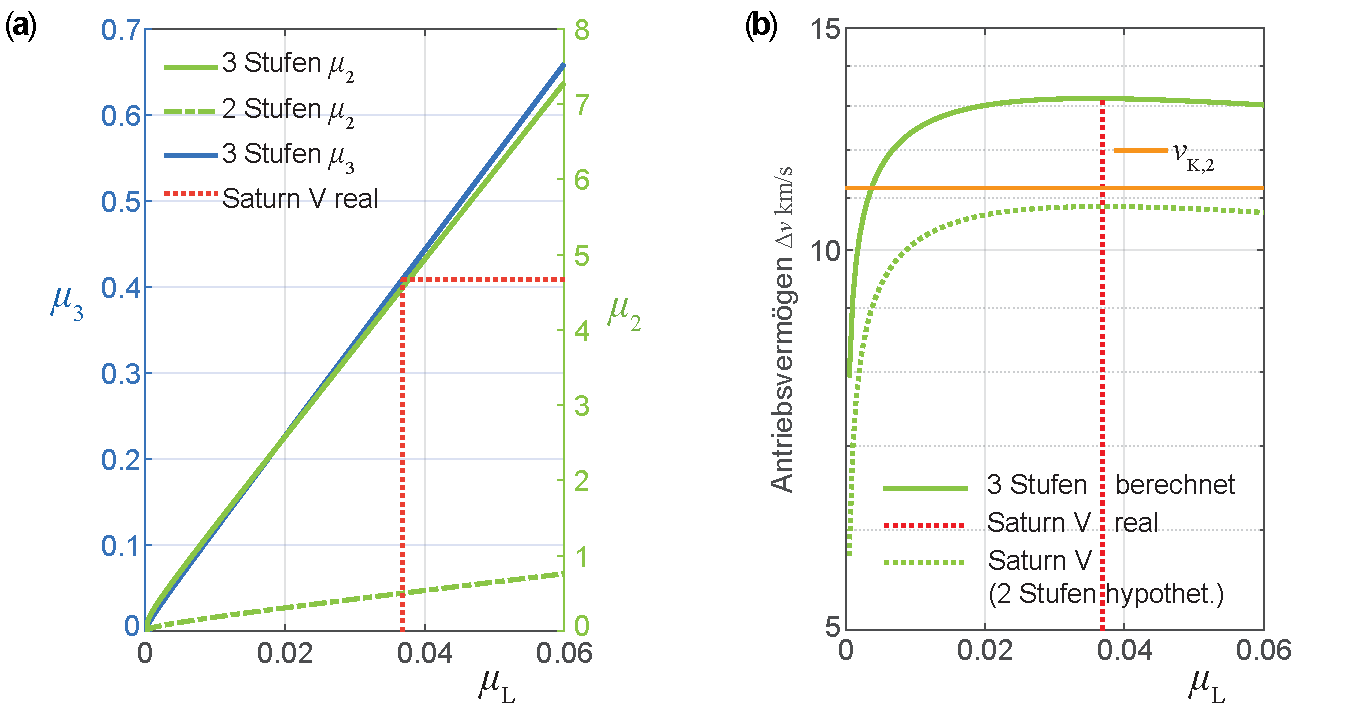
\includegraphics[width=\textwidth]{RaketenOptimierung01.pdf} 
	\caption[Optimierung einer Dreistufen-Rakete.]{Optimierung einer Dreistufen-Rakete. L�sung �ber Extremwertberechnung. \fa Berechnung der Massenverh�ltnisse der einzelnen Raketenstufen \fb Antriebsverm�gen f�r eine Dreistufen-Rakete (berechnet) und f�r die Saturn V. Zum Vergleich sind auch die Werte f�r eine (hypothetische) Ausf�hrung der Saturn V als Zweistufen-Rakete gezeigt.}
	\label{abb:adyn_optrockets01}
\end{figure}

\item \textit{\textbf{L�sungsansatz �ber Lagrange-Multiplikatoren - Beispiel Saturn V zum Mond}}\\ 
	
	Gegeben seien nach Aufgabenstellung: $v_{\text{G},i}$ (Ausstr�mgeschwindigkeit), $\sigma_i$ (Strukturparameter) und $m_0$ (Gesamtmasse der Rakete) \\
Variiert werden k�nnen die Massenverh�ltnisse $\mu_i$ oder, was gleichbedeutend ist, die Teil-Nutzlastverh�ltnisse $\eta_i$, die wir �ber
\begin{align}
    \eta_i = \frac{m_{\text{L},i}}{m_{0,i}-m_{0,i+1}} = \frac{m_{0,i+1}}{m_{\text{S},i} + m_{\text{T},i}} \label{adyn_optrocket11}
\end{align}
definieren. \\
Als $i$-tes Nutzlastverh�ltnis wird die Masse der n�chsten $\lk i+1\rk$-ten Unterrakete im Verh�ltnis zur Summe von Struktur- und Treibstoffmasse der $i$-ten Stufe definiert. Die Zahl der Stufen k�nnte ebenfalls variiert werden, soll aber hier festgehalten werden. \\
Zu optimieren/maximieren sind das Gesamt-Nutzlastverh�ltnis $\mu_\text{L}$ und das Gesamt-Antriebsverm�gen $\Delta v$, also max $\mu_\text{L}\lk \Delta v\rk$ \bzw max $\Delta v\lk\mu_\text{L}\rk $.\\
In Kapitel �ber den Lagrange-Formalismus im Band I hatten wir die Methode der Lagrange-Multiplikatoren kennen gelernt, mit der man die Extremwertberechnung der Wirkung $S$ bei Vorliegen von Zwangsbedingungen \bzw Nebenbedingungen durchf�hren konnte. Wir wenden dies f�r unser Problem an. Der Wirkung $S$ entspricht hier die Gr��e $\mu_\text{L}$ \bzw $\Delta v$, die Nebenbedingungen sind duch die $m_{\text{S},i}$ \bzw $\sigma_{i}$ gegeben und die "`Bewegungsgleichungen"' ergeben sich dann durch:
\begin{align}
    \frac{\d\lk\mu_\text{L}\rk}{\d \eta_j} + \lambda_{\mu_\text{L}}\,\frac{\d\lk \Delta v\rk}{\d \eta_j} = 0 ~~~~ \text{(maximieren von $\mu_\text{L}$)} \label{adyn_optrocket12}
\end{align}
\bzw
\begin{align}
    \frac{\d\lk\Delta v\rk}{\d \eta_j} + \lambda_{\Delta v}\,\frac{\d\lk \mu_\text{L}\rk}{\d \eta_j} = 0 ~~~~ \text{(maximieren von $\Delta v$)} \,.\label{adyn_optrocket13}
\end{align}
F�r $\lambda_{\mu_\text{L}} = 1/\lambda_{\Delta v}$ beschreiben beide Gleichungen das gleiche mathematische Problem.\\
Wir f�hren die Ableitungen aus und erhalten:
\begin{align}
\begin{split}
     \frac{\d\lk\Delta v\rk}{\d \eta_j} &= -v_{\text{G,j}}\,\frac{1-\sigma_j}{1+\eta_j}\,\frac{1}{\sigma_j+\eta_j} \,,\\
     \frac{\d\lk\mu_\text{L}\rk}{\d \eta_j}  &= \frac{\mu_\text{L}}{\eta_j\lk 1+\eta_j\rk}
\end{split}\label{adyn_optrocket14}
\end{align}
und erhalten aus \eqref{adyn_optrocket12}
\begin{align}
    \frac{\mu_\text{L}}{\eta_j\lk 1+\eta_j\rk} = \lambda_{\mu_\text{L}}\,v_{\text{G},j}\,\frac{1-\sigma_j}{1+\eta_j}\,\frac{1}{\sigma_j + \eta_j} \label{adyn_optrocket15} \,.
\end{align}
Daraus folgt sofort
\begin{align}
    v_{\text{G},j}\,\eta_j\,\frac{1-\sigma_j}{\sigma_j + \eta_j} = \frac{\mu_\text{L}}{\lambda_{\mu_\text{L}}} =:\gamma = \text{const} ~~~~ j=1,2,\ldots,N \,.\label{adyn_optrocket16}
\end{align}
Damit haben wir die Grundgleichungen f�r die Optimierung. \\
$\gamma$ ist noch eine unbekannte Gr��e, die es aus \eqref{adyn_optrocket16} zu bestimmen gilt. Wir nehmen diese zun�chst als bestimmt an, so dass sich dann die optimalen Nutzlastverh�ltnisse ergeben zu:
\begin{align}
    \eta_\text{j,\text{opt}} = \frac{\gamma\,\sigma_j}{\lk 1-\sigma_j\rk\,v_{\text{G},j}-\gamma}~~~~ j=1,2,\ldots,N \,.\label{adyn_optrocket17}
\end{align}
Wir setzen diese in die Raketen-Gleichung f�r die serielle Stufung \eqref{eq:adyn_rockets17} ein und erhalten:
\begin{align}
    \Delta v = \sum\limits_{j=1}^N\,v_{\text{G},j}\,\ln\,\frac{1+\eta_j}{\sigma_j + \eta_j} = \sum\limits_{j=1}^Nv_{\text{G},j}\,\ln\,\frac{v_{\text{G},j}-\gamma}{\sigma_j\,v_{\text{G},j}}\,.\label{adyn_optrocket18}
\end{align}
F�r das totale Nutzlastverh�ltnis 
\begin{align}
    \mu_\text{L} = \frac{m_\text{L}}{m_0} = \prod\limits_{j=1}^N\frac{\eta_j}{1+\eta_j} = \prod\limits_{j=1}^N \frac{\gamma\,\sigma_j}{\lk 1-\sigma_j\rk\lk v_{\text{G},j}-\gamma\rk}\,.\label{adyn_optrocket19}
\end{align}
Der weitere Weg besteht darin, dass man aus \eqref{adyn_optrocket18} f�r bekannte $\sigma_j$, $\Delta v$ die Konstante $\gamma$ (die aus dem Lagrange-Multiplikator abgeleitet wurde) bestimmt und diese in \eqref{adyn_optrocket19} einsetzt, um $\mu_\text{L,opt}$ zu erhalten. \\
Die Konstante $\gamma$ muss aus der Gleichung \eqref{adyn_optrocket16} numerisch bestimmt werden, was wir vorteilhaft in \matlab\,im Skript \mladynref{RaketenOptimierung02.m} ausgef�hrt haben.\\
Wenn wir die in der �bung in Tabelle \ref{tab:adyn_parameter_Apollo11} angegebenen Werte verwenden, erhalten wir aus der Rechnung einen Wert von $\mu_\text{L} = 0.0176$, der nur wenig von dem tats�chlichen (etwas kleineren) Wert von $\mu_\text{L} = 0.0162$ abweicht, mit dem die NASA (vermutlich aus Sicherheitsgr�nden) operierte.
In \figref{adyn_optrockets02} ist das maximale Nutzlastverh�ltnis gezeigt, mit der eine Nutzlast von $m_\text{L} = \mu_\text{L,opt}\cdot m_0$ auf ein bestimmtes Antriebsverm�gen gebracht werden kann.\\
Es sei noch darauf hingewiesen, dass $\gamma < \mathrm{min}\lk v_{\text{G},j}\,\lk 1-\sigma_j\rk \rk \,$f�r alle $j=1,\ldots,N$ sein muss, was bei der numerischen Berechnung zu ber�cksichtigen ist.
	
\begin{figure}[H]
	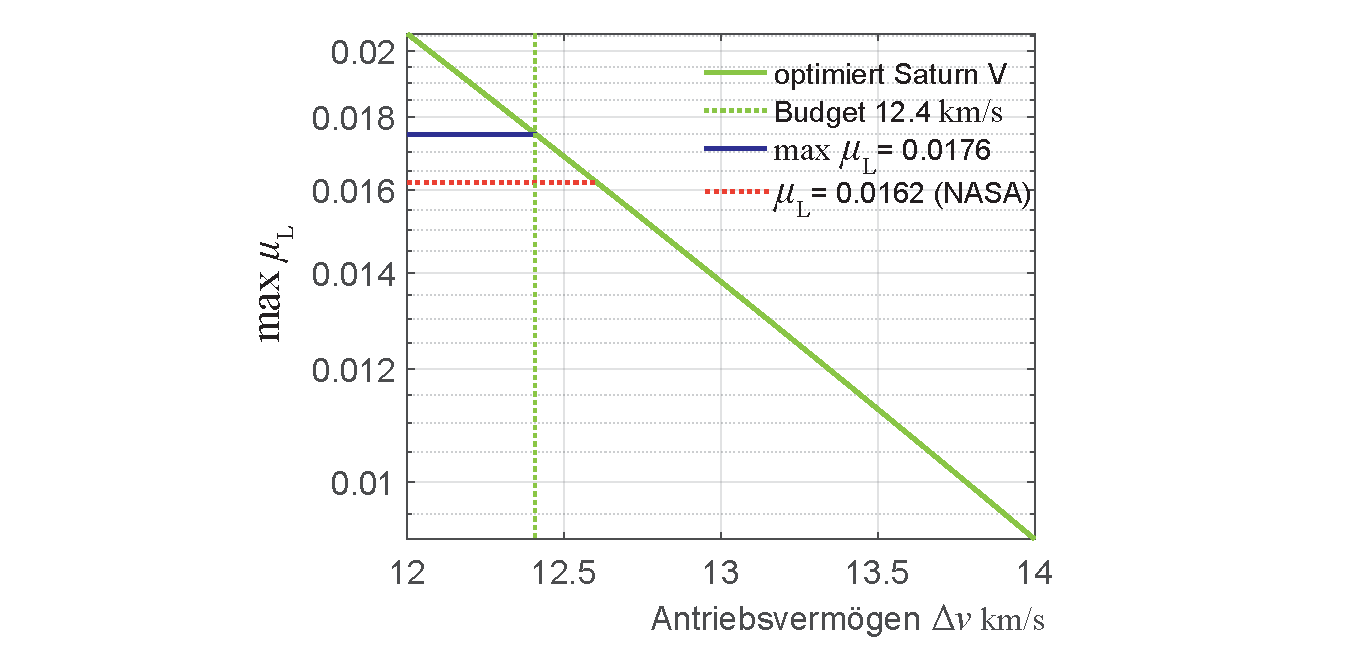
\includegraphics[width=\textwidth]{RaketenOptimierung02.pdf} 
	\caption[Optimierung einer Dreistufen-Rakete.]{Optimierung Saturn V Konfiguration f�r die Apollo Missionen. L�sung �ber Methode der Lagrange-Multiplikatoren. Berechnung des optimalen Antriebsverm�gens/Nutzlastverh�ltnisses.}
	\label{abb:adyn_optrockets02}
\end{figure}


\end{enumerate}

\end{sol} 
\textcolor{blue} {$\rightarrow$ zur} \probref{adyn_rocketopt1}.\\
\noindent\rule[1ex]{\textwidth}{0.5pt}  \newpage  \clearpage


%-----------------------------------------------------------------------------------------------------------


\begin{sol}{prob:adyn_rocketopt2}\label{lsg:adyn_rocketopt2} %�bung4
\textbf{Vergleich Mehrstufenrakete (Serielle und Parallelstufung)} \\ \\
Wir fassen die Vor- und Nachteile der Tandemstufung gegen�ber der Parallelstufung  in der folgenden Tabelle zusammen.\\
\begin{table}%tab1
\caption{Vor- und Nachteile der Tandemstufung gegen�ber der Parallelstufung.}
\smallskip
\hspace{1.5cm}
\begin{tabular}{L{3cm}L{3cm}L{3cm}}
\svhline\noalign{\smallskip}
Eigenschaft				    			& Tandemstufung				& Parallelstufung \\
\noalign{\smallskip}\svhline\noalign{\smallskip}
\noalign{\smallskip}
Startbeschleunigung							&kleiner &gr��er\\	
Strukturbelastung 							&kleiner &gr��er\\	
Biegemomente      							&gr��er  &kleiner\\	
Aerodynamische Verluste 				&kleiner &gr��er\\	
Gravitationsverluste						&gr��er  &kleiner\\	
Gesamtl�nge Rakete							&gr��er  &kleiner\\	
\noalign{\smallskip}
\svhline\noalign{\smallskip}
\end{tabular} \\
\label{tab:adyn_vergleich_staging}
\end{table}%tab1


\end{sol} 
\textcolor{blue} {$\rightarrow$ zur} \probref{adyn_rocketopt2}.\\
\noindent\rule[1ex]{\textwidth}{0.5pt}  \newpage  \clearpage


%-----------------------------------------------------------------------------------------------------------


%-----------------------------------------------------------------------------------------------------------
%-----------------------------------------------------------------------------------------------------------

\subsection{�bungen zu Umlaufbahnen}

\medskip

%-----------------------------------------------------------------------------------------------------------

\begin{sol}{prob:adyn_orbits1}\label{lsg:adyn_orbits1} %�bung5
\textbf{Bahnparameter aus Bodenbeobachtungen}\\ \\
\textit{Bahnparameter von Satelliten mit gegebenen geozentrischen Orts- und Geschwindigkeitsdaten:}\\ \\
Wir verwenden die Formeln aus \kap{adyn_orbits_determination_rv} und erhalten:\\

Satellit 1 (HEO)
\begin{align*}
	&\text{Halbachse}\,\,a & \SI{20251.57}{\km}\\
	&\text{Exzentrizit�t}\,\,e & 0.777596\\
	&\text{Bahnneigung} \,\,i &   10.194 \degree\\
	&\text{Knoten} \,\, \Omega &  171.951 \degree\\
	&\text{Arg. Perig�um} \,\, \omega &  86.081 \degree\\
	&\text{Mittl. Anomalie} \,\, M &  138.824  \degree\\
	&\text{Mittl. Bewegung} \,\, n & \SI{2.19e-04}{\per\second} \\
\end{align*}

Satellit 2 (LEO)
\begin{align*}
	&\text{Halbachse}\,\,a & \SI{8225.40}{\km}\\
	&\text{Exzentrizit�t}\,\,e & 0.076722\\
	&\text{Bahnneigung} \,\,i &   6.707 \degree\\
	&\text{Knoten} \,\, \Omega &  145.881 \degree\\
	&\text{Arg. Perig�um} \,\, \omega &  86.476 \degree\\
	&\text{Mittl. Anomalie} \,\, M &  167.278  \degree\\
	&\text{Mittl. Bewegung} \,\, n & \SI{8.46e-04}{\per\second}
\end{align*}

\newpage

\textit{Bahnparameter der ISS aus den ver�ffentlichten geozentrischen Orts- und Geschwindigkeitsdaten der NASA:}\\
	%\url{https://spotthestation.nasa.gov/trajectory_data.cfm}\\

Auch hier verwenden wir die Formeln aus \kap{adyn_orbits_determination_rv} und erhalten:
\begin{align*}
	&\text{Halbachse}\,\,a & \SI{6803.28}{\km}\\
	&\text{Bahnh�he}\,\,h & \SI{425.28}{\km}\\
	&\text{Exzentrizit�t}\,\,e & 0.001855\\
	&\text{Bahnneigung} \,\,i &  51.751 \degree\\
	&\text{Knoten} \,\, \Omega &  47.685 \degree\\
	&\text{Arg. Perig�um} \,\, \omega & 124.00 \degree\\
	&\text{Mittl. Anomalie} \,\, M & 315.75 \degree\\
	&\text{Umlaufzeit} \,\, n & \SI{93.8 }{\minute}
\end{align*}
Die mittlere Anomalie $M$ wurde so angepasst, dass der Anfangswert mit den NASA Daten �bereinstimmt. Wir verweisen auf \kap{adyn_orbits_determination_singulaer}
zur Berechnung alternativer Bahnparameter bei kreisf�rmigen und �quatorialen Bahnen, sowie auf die Zusatzaufgabe \probref{adyn_orbits_zusatz1}.
\begin{figure}[H]
	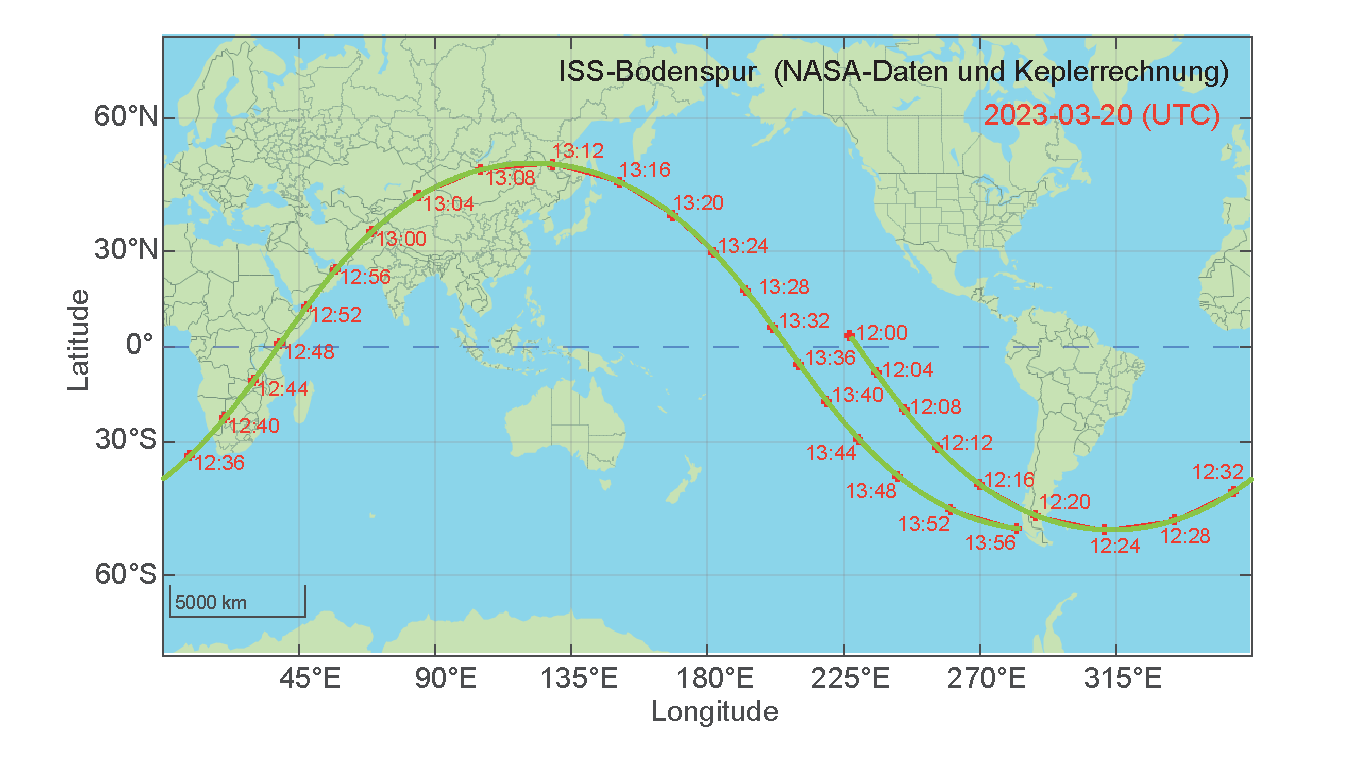
\includegraphics[width=\textwidth]{GroundTrackISS20032023.pdf} 
	\caption[Bodenspur der ISS.]{Bodenspur der ISS. Vergleich NASA Daten und Berechnung Keplerbahn.}
	\label{abb:adyn_satobserv02}
\end{figure}
Die Berechnungen finden sich im Detail im \mscr{} \mladynref{BahnparaBestimmung01.m}. 

\end{sol} 
\textcolor{blue} {$\rightarrow$ zur} \probref{adyn_orbits1}.\\
\noindent\rule[1ex]{\textwidth}{0.5pt}  \newpage  \clearpage

%-----------------------------------------------------------------------------------------------------------
\newpage

\begin{sol}{prob:adyn_orbits2}\label{lsg:adyn_orbits2} %�bung6
\textbf{Bodenspuren von Erdsatelliten}\\ 

\begin{itemize}
	\item \textit{\textbf{Bodenspuren verschiedener Satellitenarten}}\\
		\begin{itemize}
			\item Bodenspur eines GEO-Satelliten.
			\item Bodenspur eines Molnija-Satelliten (HEO-Satelliten).
			\item Bodenspur eines polaren Satelliten. 
		\end{itemize}
		\begin{figure}[H]
			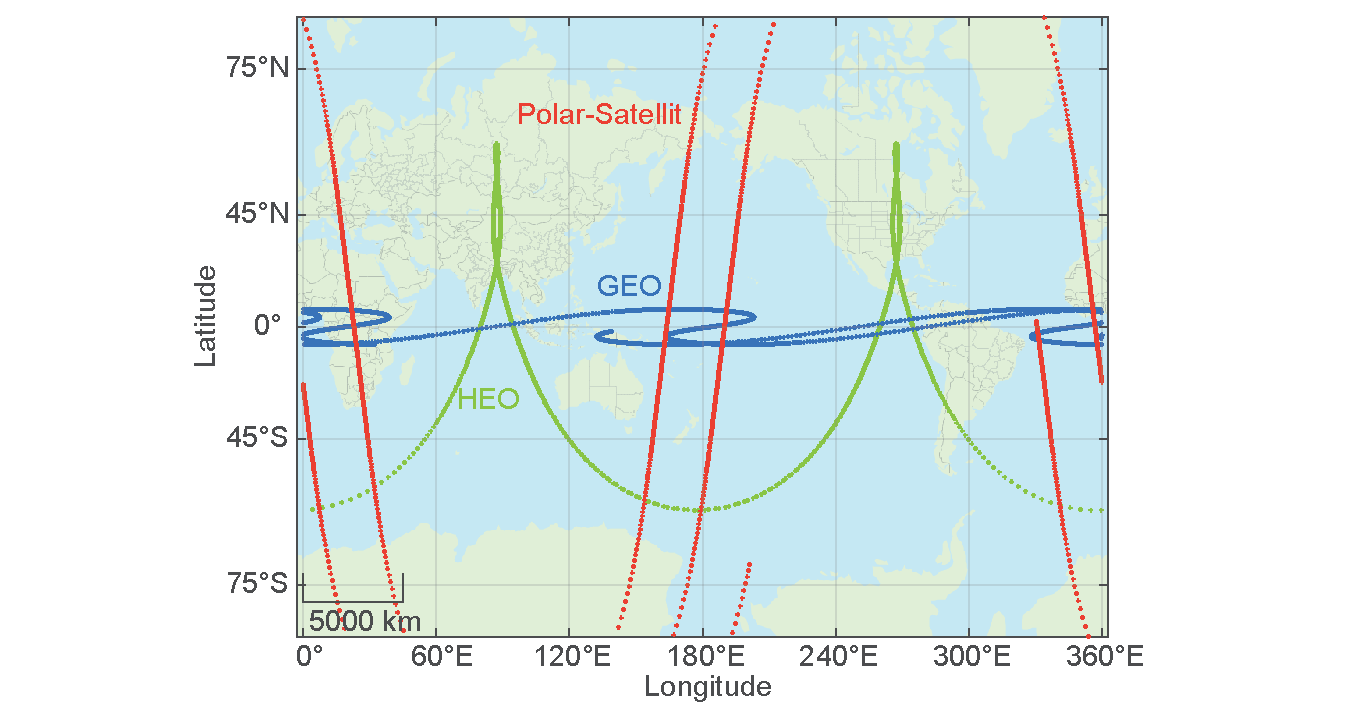
\includegraphics[width=0.9\textwidth]{Orbits03a.pdf} 
			\caption[Bodenspuren von verschiedenen Satelliten.]{Bodenspuren von verschiedenen Satelliten. GEO:\, $a = \SI{25000}{\km},\, e = 0.73,\, i = 8\degree,\, \Omega =45\degree$,\,\, HEO (Typ Molnija-Satelliten):\, $a = \SI{26555}{\km},\, e = 0.72,\, i = 63.4\degree,\, \Omega =120\degree,\,\omega =270\degree$,\,\, Polar-Satellit:\, $a = \SI{7330}{\km},\, e = 0.0,\, i = 93\degree,\, \Omega =130\degree,\,\omega =0\degree$.}
			\label{abb:adyn_orbits03a}
			\end{figure}
	\item \textit{\textbf{Bodenspuren verschiedener Satelliten in geosynchronen Umlaufbahnen}}\\

				Die Bodenspuren \figref{adyn_orbits03b} �hneln den verschiedenen Analemma, die wir im \kap{kulmination_sonne} \bzw in der \probref{hm_Analemma_Mars} kennen gelernt hatten. Das ist nicht verwunderlich. In einer geozentrischen Betrachtung �bernehmen die Satelliten die Rolle der Sonne, die unterschiedlichen Formen des \textit{\anf{Satelliten-Analemmas}} kommen durch die unterschiedlichen Bahnparameter zustande. Siehe auch im Detail \probref{hm_Analemma_Mars}.\\
\newpage
			\begin{figure}[H]
			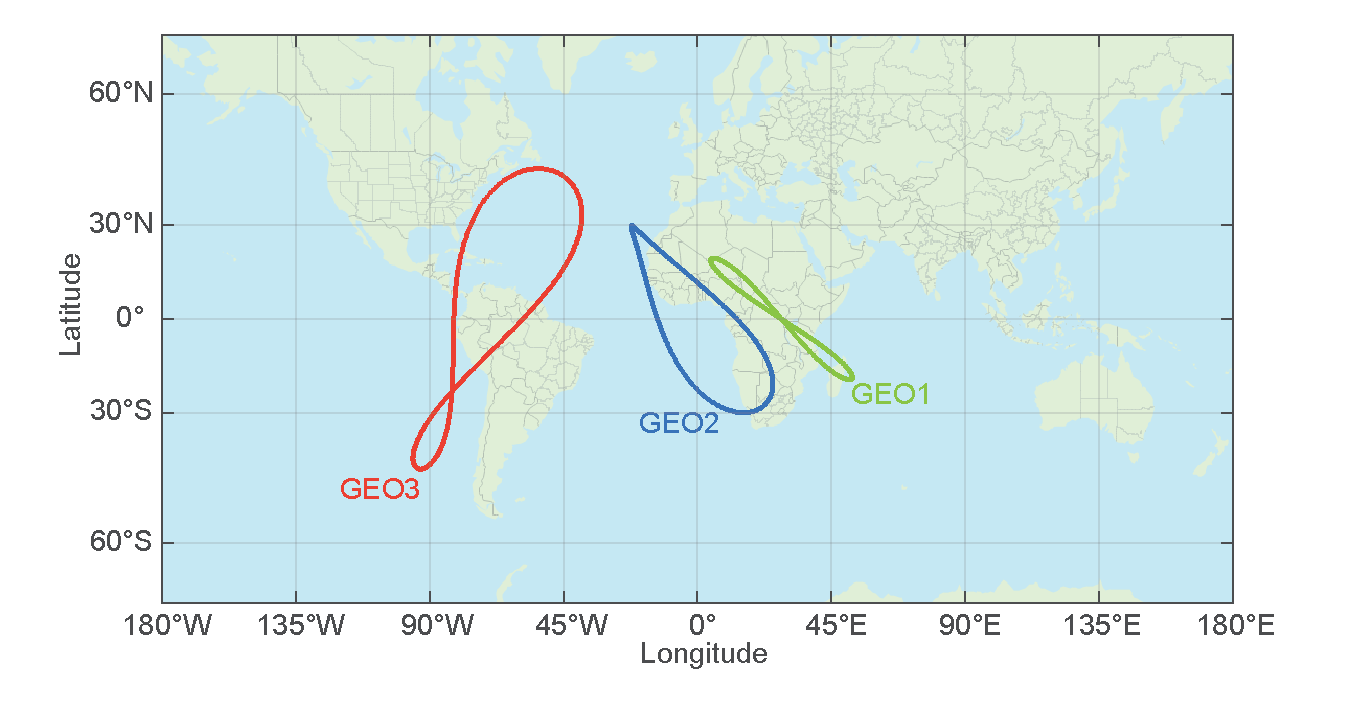
\includegraphics[width=0.95\textwidth]{Orbits03b.pdf} 
			\caption[Bodenspuren von verschiedenen geosynchronen Satelliten.]{Bodenspuren von verschiedenen geosynchronen Satelliten. Parameter siehe \probref{adyn_orbits2}.}
			\label{abb:adyn_orbits03b}
			\end{figure}
\item \textit{\textbf{Bodenspur ISS}}\\
			\begin{figure}[H]
			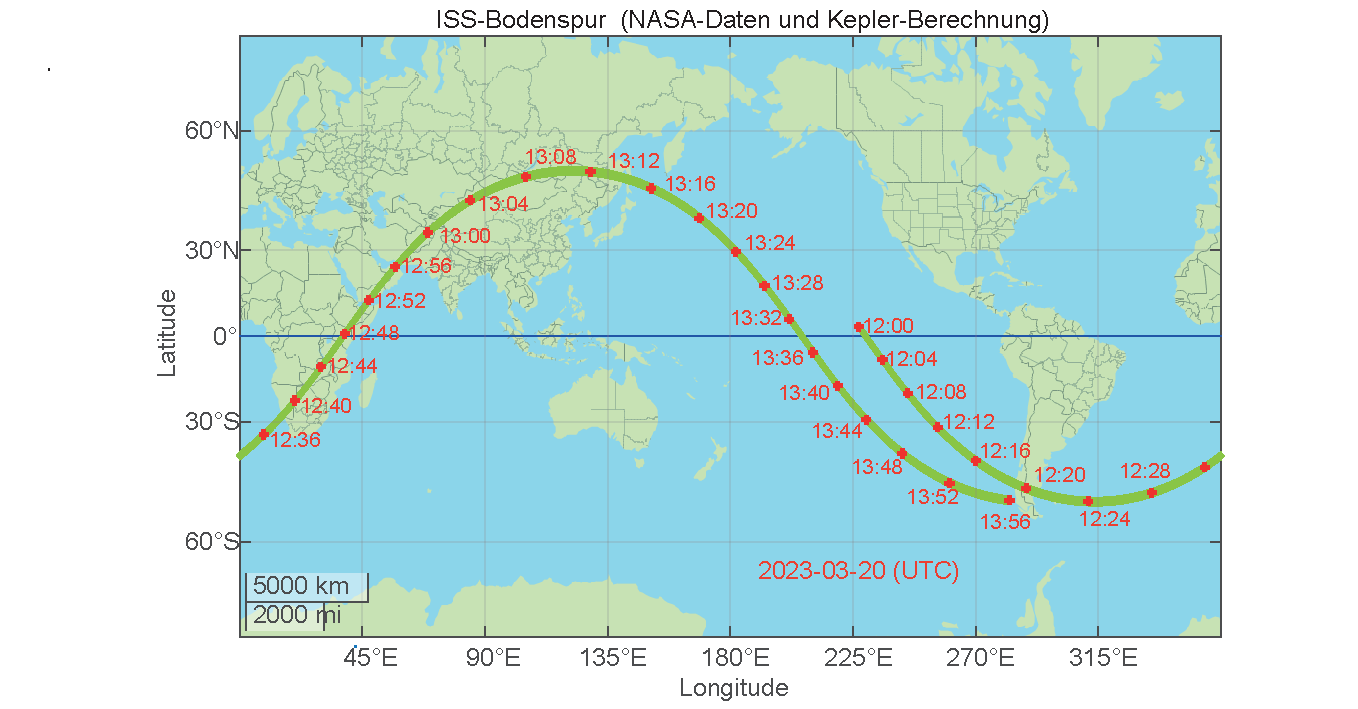
\includegraphics[width=0.95\textwidth]{ISSBodenspur.pdf} 
			\caption[Bodenspuren der ISS.]{Bodenspuren der ISS vom 20.03.2023. Parameter siehe \probref{adyn_orbits2}.}
			\label{abb:adyn_orbits03c}
			\end{figure}
\end{itemize}
Die Berechnungen finden sich im Detail im \mscr~\mladynref{SatPositionen01.m} \bzw \mladynref{SatPositionen02.m}.

\end{sol} 
\textcolor{blue} {$\rightarrow$ zur} \probref{adyn_orbits2}.\\
\noindent\rule[1ex]{\textwidth}{0.5pt}  \newpage  \clearpage

%-----------------------------------------------------------------------------------------------------------

\begin{sol}{prob:adyn_orbits3}\label{lsg:adyn_orbits3} %�bung7
\textbf{Bodenbeobachtung von Erdsatelliten}\\ \\

Die Berechnungen finden sich im Detail im \mscr~\mladynref{SatPositionen03.m} \bzw \mladynref{SatPositionen04.m}.
\begin{figure}[H]
	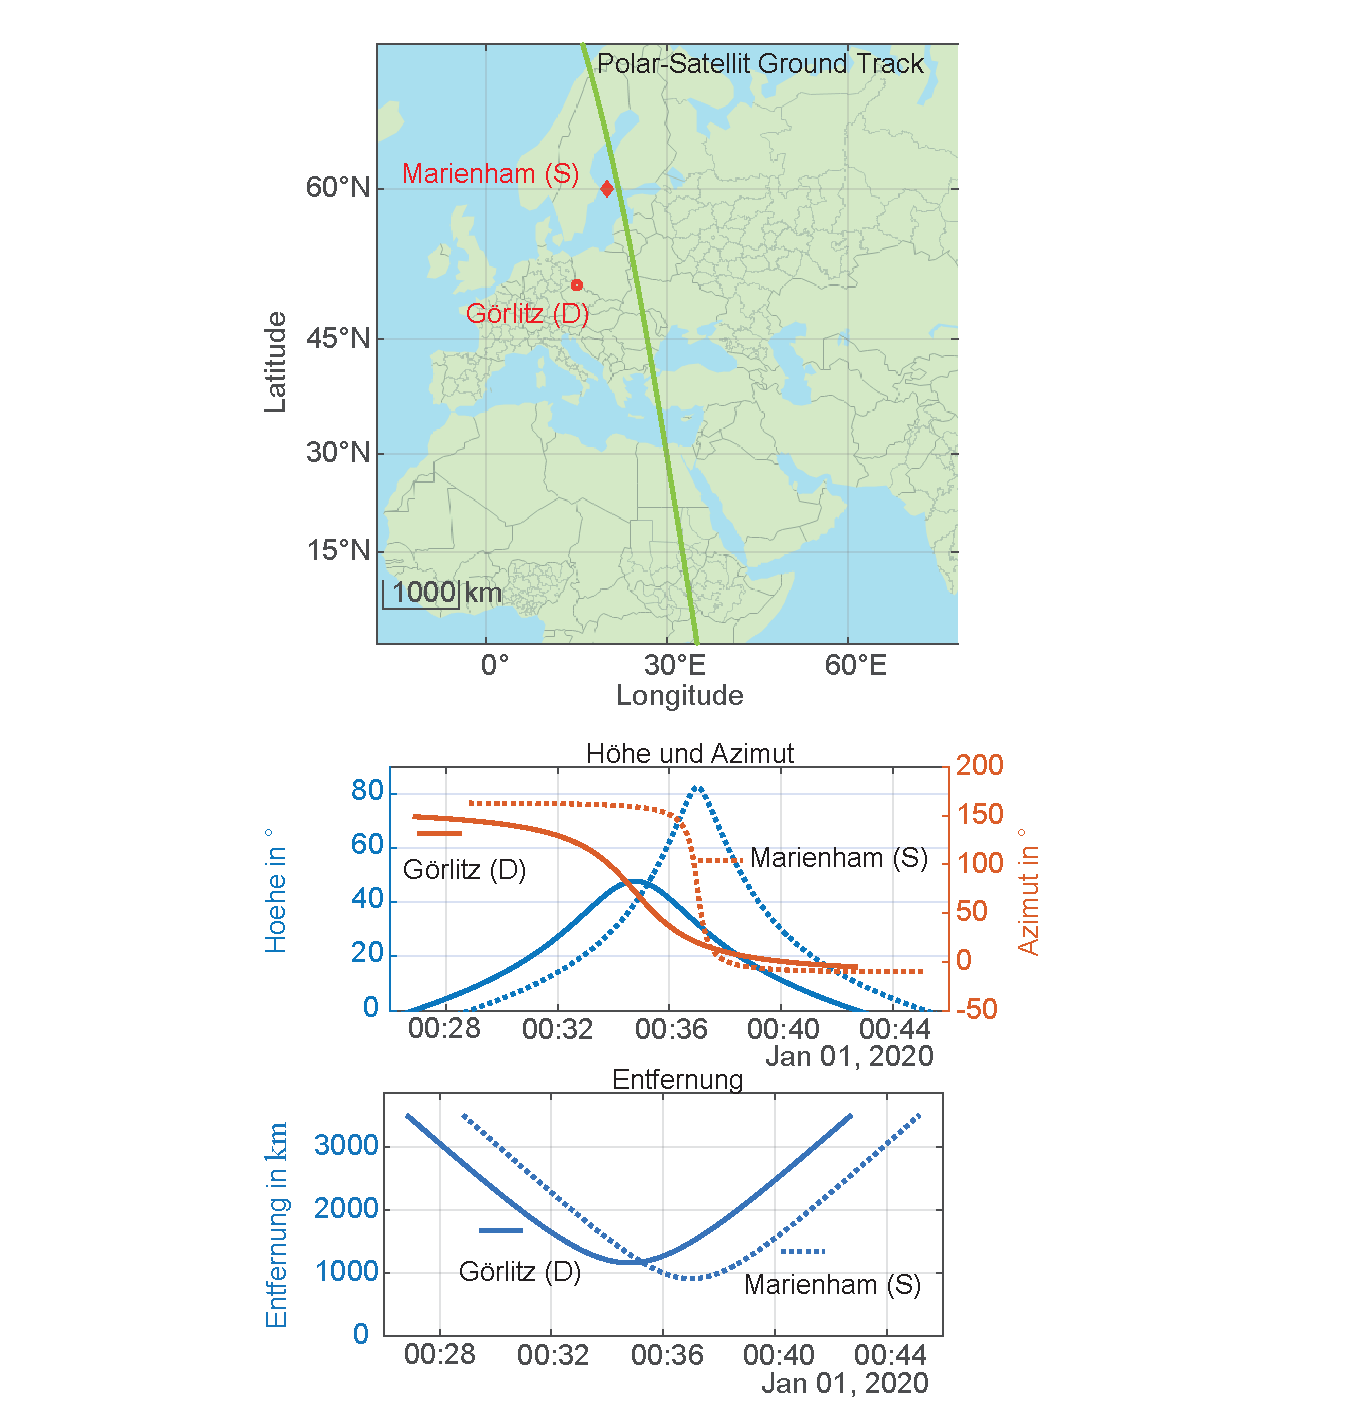
\includegraphics[width=\textwidth]{TopographPolarerSat.pdf} 
	\caption[Topographische Beobachtung eines polaren Satelliten.]{Bodenspur, Azimut, H�he und Entfernung eines polaren Satelliten von zwei Bodenstationen. Parameter siehe \probref{adyn_orbits3} und \mscr~\mladynref{SatPositionen03.m} \bzw \mscr~\mladynref{SatPositionen03a.m}.}
	\label{abb:adyn_satobserv03}
\end{figure}
\begin{figure}[H]
	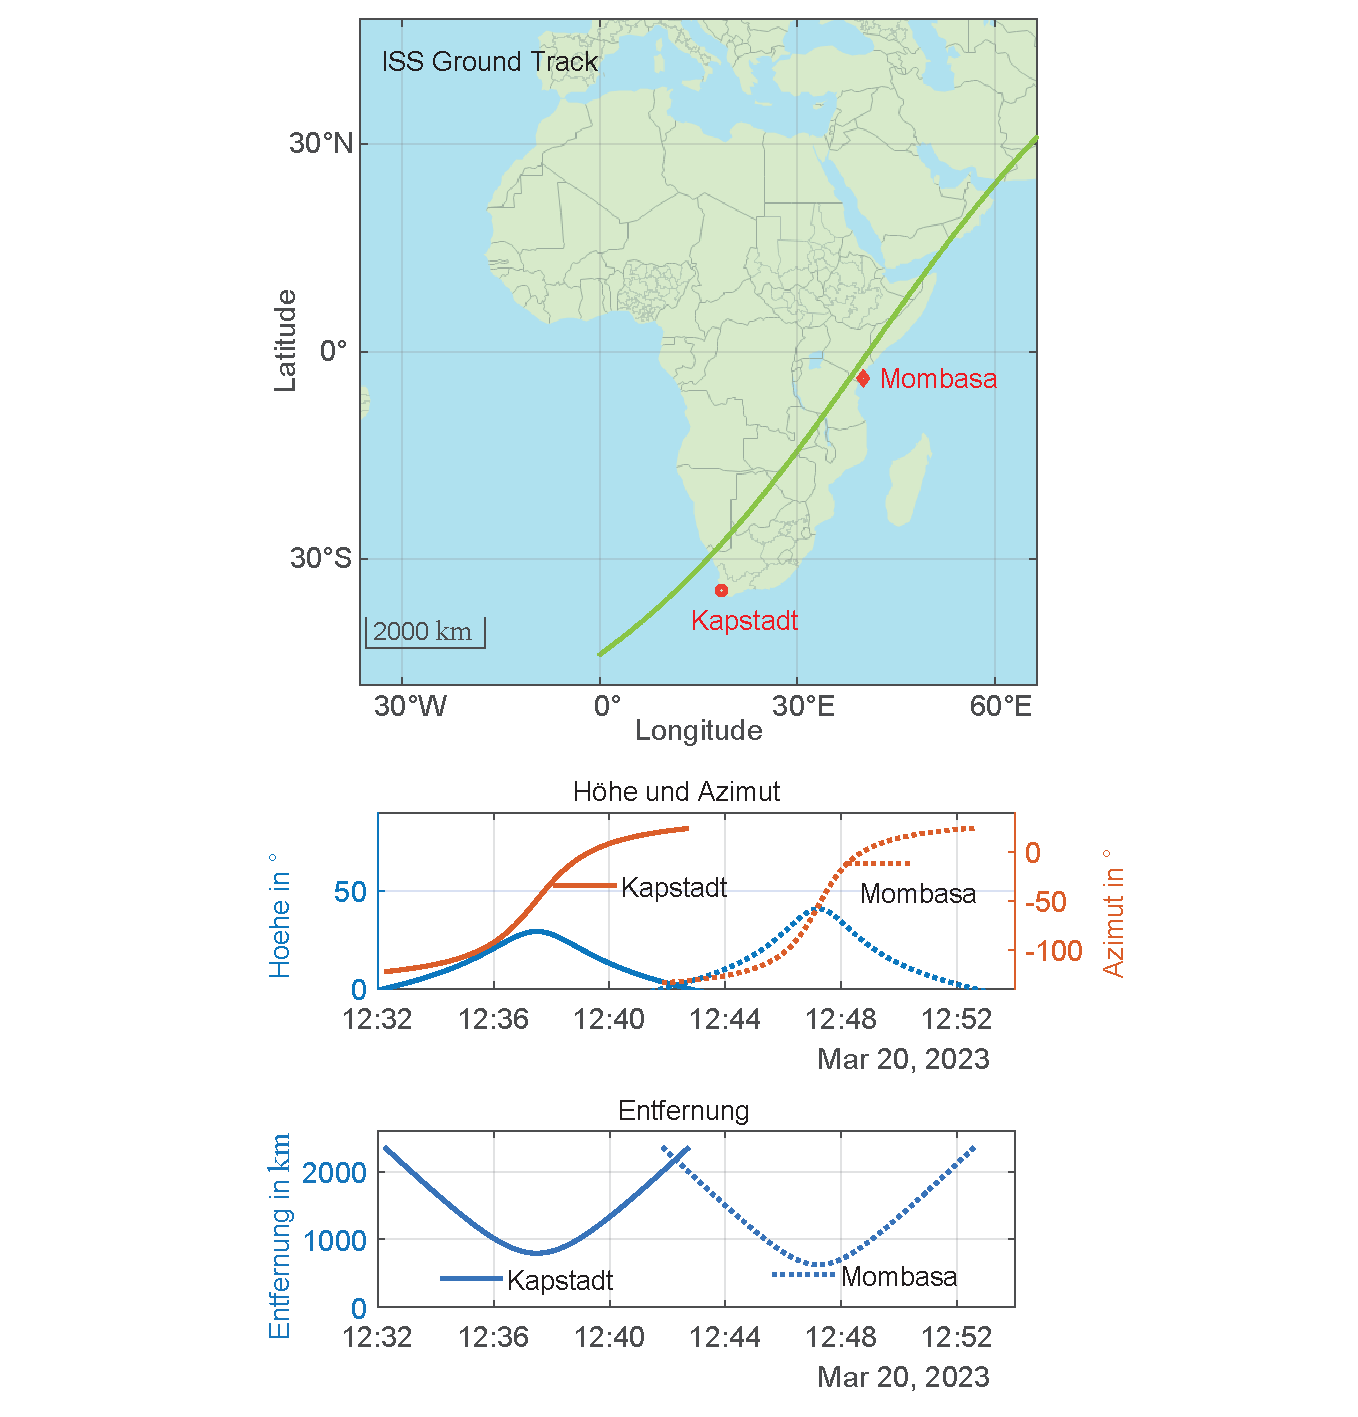
\includegraphics[width=\textwidth]{TopographISS.pdf} 
	\caption[Topographische Beobachtung der ISS.]{Bodenspur, Azimut, H�he und Entfernung der von zwei Bodenstationen. Parameter siehe \probref{adyn_orbits3} und \mscr~\mladynref{SatPositionen04.m}.}
	\label{abb:adyn_satobserv04}
\end{figure}

\end{sol} 
\textcolor{blue} {$\rightarrow$ zur} \probref{adyn_orbits3}.\\
\noindent\rule[1ex]{\textwidth}{0.5pt}  \newpage  \clearpage

%-----------------------------------------------------------------------------------------------------------

\begin{sol}{prob:adyn_orbits4}\label{lsg:adyn_orbits4} %�bung8
\textbf{Bodenbeobachtung eines Molniya-Satelliten}\\ \\

Die Berechnungen finden sich im Detail im \mscr~\mladynref{SatPositionen05.m}.
\begin{figure}[H]
	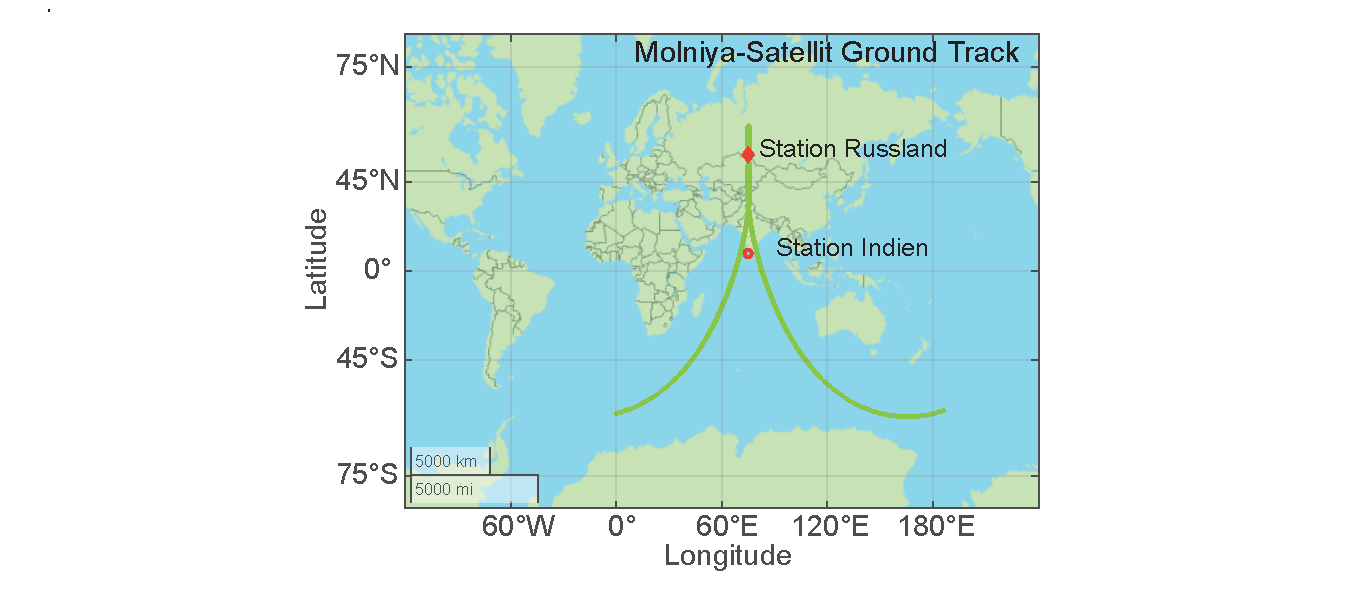
\includegraphics[width=\textwidth]{TopographMolniyaSat01.pdf} 
	\caption[Bodenspur eines Molniya-Satelliten.]{Bodenspur eines Molniya-Satelliten.\\Parameter siehe \probref{adyn_orbits4} und \mscr~\mladynref{SatPositionen05.m}.}
	\label{abb:adyn_MolniyaObserv01}
\end{figure}
\begin{figure}[H]
	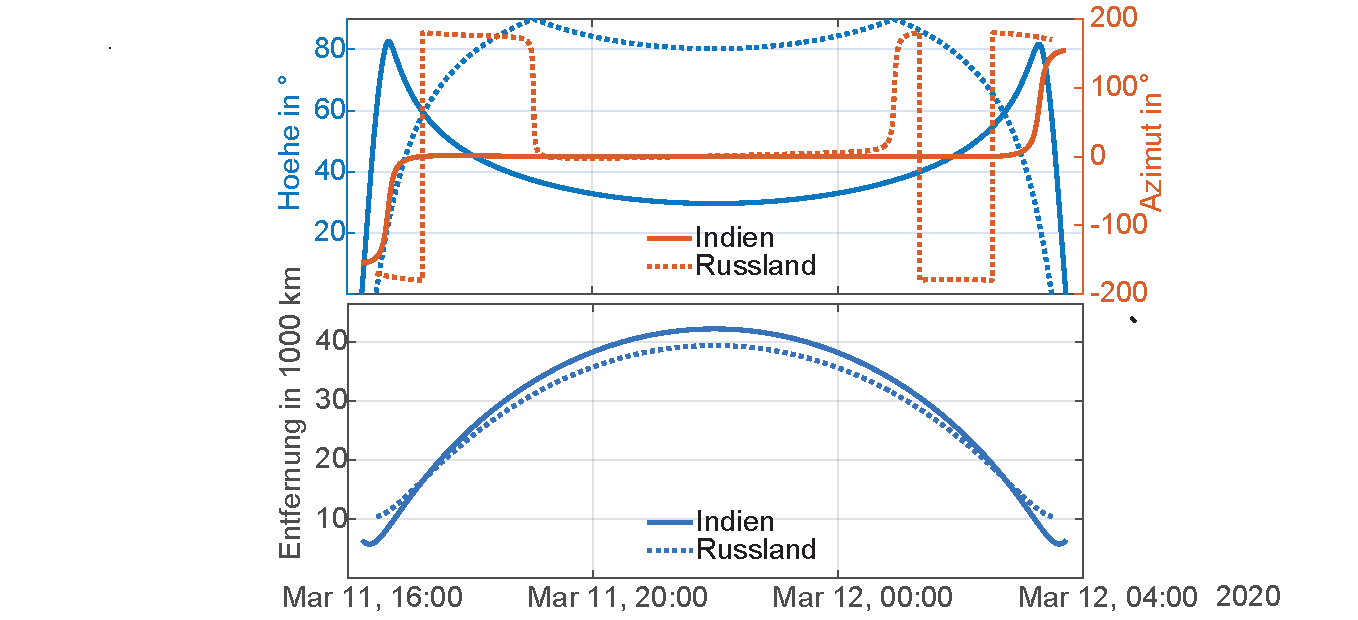
\includegraphics[width=\textwidth]{TopographMolniyaSat02.pdf} 
	\caption[Topographische Beobachtung eines Molniya-Satelliten.]{Azimut, H�he und Entfernung eines Molniya-Satelliten von zwei Bodenstationen. Parameter siehe \probref{adyn_orbits4} und \mscr~\mladynref{SatPositionen05.m}.}
	\label{abb:adyn_MolniyaObserv02}
\end{figure}
\end{sol} 
\textcolor{blue} {$\rightarrow$ zur} \probref{adyn_orbits4}.\\
\noindent\rule[1ex]{\textwidth}{0.5pt}  \newpage  \clearpage


%-----------------------------------------------------------------------------------------------------------

\begin{sol}{prob:adyn_orbits5}\label{lsg:adyn_orbits5} %�bung9
\textbf{Sonnensynchrone Bahnen}\\ \\

Die Drehimpulserhaltung gilt streng nur f�r das Zweik�rperproblem, dann ist auch die Bahnebene fest im Raum orientiert und die Bahn geschlossen.\\
Wie wir \zb in \kap{Periheldrehung} gesehen haben, bewirkt die Abplattung der Erde jedoch ein Drehmoment auf die Bahn und f�hrt zu einer Verschiebung der Rektaszension des aufsteigenden Knotens. 
Man kann mit Hilfe der St�rungsrechnung zeigen (siehe auch \probref{adyn_pertubations}), dass die Frequenz dieser Pr�zession des aufsteigenden Knoten sich nach folgender Formel berechnet:
	\begin{align}
		\dot{\Omega} = -\frac{3}{2} J_2\, \frac{2\pi}{T_\text{E}} \lk \frac{R_\text{E}}{a\,(1-e^2)} \rk^2 \cos i = 
		-\frac{3}{2} J_2\,R_\text{E}\, \sqrt{\frac{a_\text{E}}{a_\text{E}{}^2}} \, \frac{\cos i}{a^2\,(1-e^2)^2} = C\,f(a,e,i)\,. \label{eq:adyn_orbits5_01}
	\end{align}
Hierin sind $J_2$ die sogenannte zonale Harmonische\index{Harmonische!zonale} (siehe \kap{adyn_gravity_pertubations}) als Ma� f�r die Abplattung der Erde, $R_\text{E}$ der mittlere Erdradius, $a$ die gro�e Halbachse der Satellitenbahn und $i$ \bzw $e$ deren Neigung (Inklination) \bzw Exzentrizit�t. $T_\text{E} = 2\pi\sqrt{a_\text{E}{}^3/\mu_\text{E}}$ ist die Umlaufzeit der Erde um die Sonne.\footnote{Genauer gesagt ist es die Zeit eines anomalistischen Jahres ($\SI{365.25963}{}\,\mathrm{d}$, siehe \kap{hm_zeitdefinition})} Die Pr�zession ist umso gr��er, je geringer die Inklination $i$ und die Bahnh�he $a$ sind.\\
Wegen des Minuszeichen wirkt bei einer retrograden Bahnen (Bahn entgegen der Erdrotation, \dh $i > 90\degree$) diese Pr�zession in die gleiche Richtung wie die Erdrotation. Man kann also durch geeigneter Wahl von Inklination und Flugh�hen daf�r sorgen, dass sich die Bahn gerade um so viel verschiebt wie der mittleren Bewegung der Erde ($2\pi/T_\text{E}$) um die Sonne entspricht (\figref{adyn_synchron_orbit}). 

Bei einem SSO erfolgt der �berflug des Satelliten �ber einen Punkt auf der Oberfl�che des Planeten immer zur selben Ortszeit, vorausgesetzt die geographische Breite des Ortes liegt innerhalb des Bereiches, der durch die Inklination der Bahn begrenzt wird. Aufgrund dieser konstanten �berflugszeit lassen sich Beobachtungen von verschiedenen Tagen und Jahreszeiten gut miteinander vergleichen, deswegen haben ja Wetter- und Erdbeobachtungssatelliten oft solche Bahnen.

\begin{figure}[H]
	\includegraphics[width=\textwidth]{SonnensynchroneBahn.pdf} 
	\caption[Sonnensynchrone Bahn.]{Sonnensynchrone Bahn. Symbolische und nicht-ma�stabsgetreue Darstellung. }
	\label{abb:adyn_synchron_orbit}
\end{figure}

\newpage
\textbf{Zusatzaufgabe}\\

Wir wollen nun noch die Bodenspur des ERS-1 SSO-Satelliten berechnen \cite{Gottschalk1991}. Man k�nnte nun aus \eqref{eq:adyn_orbits5_01} einen der Parameter $a,\, e$ oder $i$ berechnen und die anderen vorgeben. 
Man hat aber eben mit $a$ einen weiteren Freiheitsgrad neben $i$, womit man auch fordern kann, dass die Bahnh�he $h$ so gew�hlt wird, dass ein �berflug �ber eine Gebiet (\zb das �berkreuzen des �quators nach $K$ Tagen \bzw. $N$ Orbits genau wiederholt (sogenannte \textit{Sonnensynchrone Repeat Orbits}).  Anfangs w�hlte man f�r den ERS-1 K=3, N=43, sp�ter ging man auf K=35.
Um das zu erreichen, muss man auch die St�rungen der Perihelverschiebung (siehe \kap{Stoerpotential_Merkur}) und der mittleren Anomalie ber�cksichtigen. Diese sind f�r kreisf�rmige Bahnen gegeben durch \cite{Montenbruck2012, Murray2008, Vallado2007}:

	\begin{align}
	\begin{split}
		\dot{\omega} = -\frac{3}{4} J_2\, n_0 \frac{R_\text{E}{}^2}{a^2} \lk 1 - 5\cos^2 i\rk \\ 
    \Delta n = n - n0  = -\frac{3}{4} J_2\, n_0 \frac{R_\text{E}{}^2}{a^2} \lk 1 - 2\cos^2 i\rk\,,
	\end{split}\label{eq:adyn_orbits5_02}
\end{align}

worin $n_0=\sqrt{(GM_\text{E}/a^3)}$ die mittlere Bewegung der Kepler-Bahn ist.
F�r sonnensynchrone Bahnen ist dann gefordert, dass gilt:

	\begin{align}
		\dot{\Omega} - \dot{\theta} = -360\degree\,, \\ 
\label{eq:adyn_orbits5_03}
\end{align}

woraus man f�r die Umlaufzeit einer solchen Bahn die Beziehung

	\begin{align}
		T_\text{P,SSO} = \frac{2\pi}{n_0-\Delta n-\dot{\omega}}\,, \\ 
\label{eq:adyn_orbits5_04}
\end{align}

was etwas l�nger ist als die Umlaufzeit im reinen Kepler-Fall.
Durch Iteration mit dem Startwert $T_\text{P,SSO}^{(0)}= 2\pi/n_0$ findet man �ber \eqref{eq:adyn_orbits5_02} aus \eqref{eq:adyn_orbits5_01} nacheinander $a$ und $i$ f�r die geforderten Bedingungen.\\

Wir finden:
\begin{align} 
  h &= a - R_\text{E} = \SI{7153.1}{\km} - \SI{6371.0}{\km} = \SI{782.1}{\km}\,, \\
	i &= 98.5\degree,
\end{align}
was f�r unsere Kreisbahnn�herung gut mit den Werten in \cite{Gottschalk1991} �bereinstimmt.
F�r die Berechnung der Bodenspur zu verschiedenen Zeiten, m�ssen Sie die Zeitabh�ngigkeit von $\Omega(t) = \Omega(t_0) + \dot{\Omega}\,(t-t_0)$ beachten.\\
Die Rechnungen finden sich im Detail im \mscr~\mladynref{SonnenSynchroneBahn.m} und ein Ergebnis in \figref{adyn_synchron_groundtrack}.

\begin{figure}[H]
	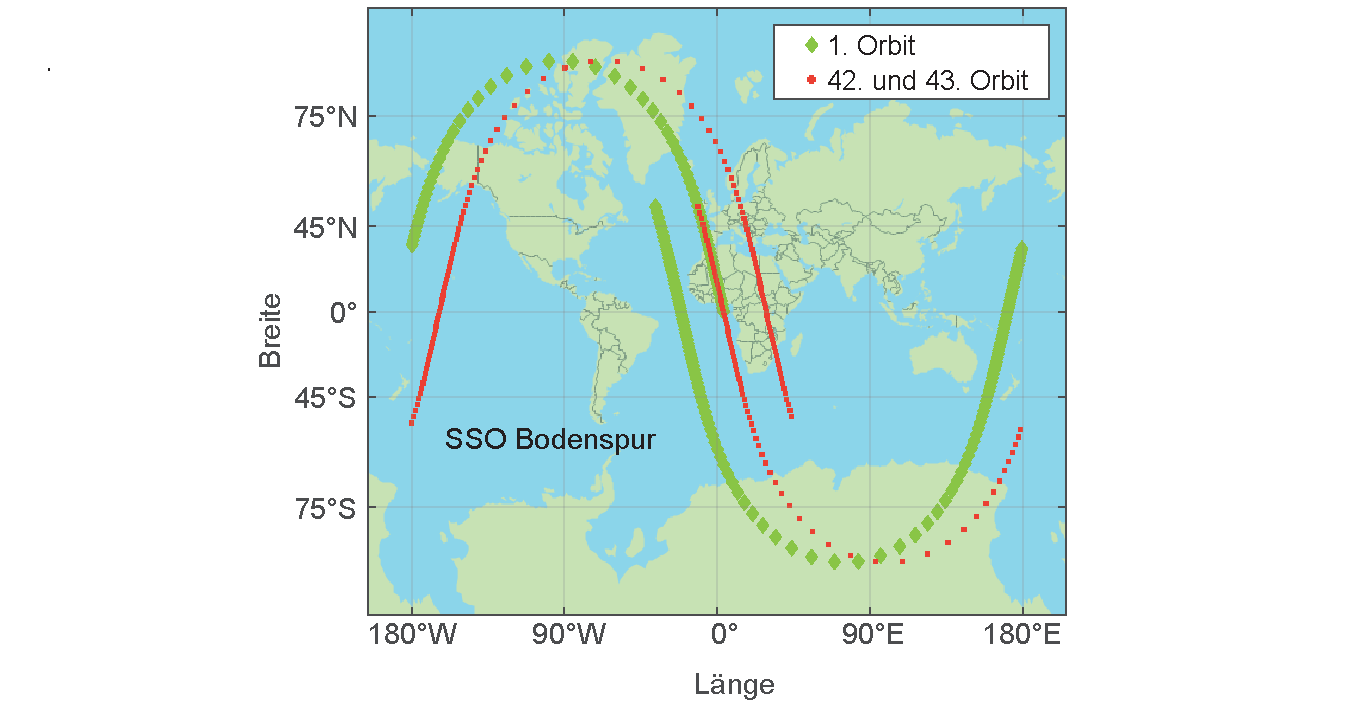
\includegraphics[width=\textwidth]{SonnensynchroneBodenspur.pdf} 
	\caption[Sonnensynchroner \textit{Repeat Orbit} -Bodenspur.]{Sonnensynchroner \textit{Repeat Orbit} - Bodenspur. Gezeigt sind Orbit Nr. 1 (willk�rlich gew�hlt) und die Orbits Nr 42 und Nr. 43 als Bodenspur. Man sieht, dass bei $N=43$ nach 3 Tagen der Satellit genau �ber die gleichen Gebiete fliegt wie beim Orbit $N=1$.}
	\label{abb:adyn_synchron_groundtrack}
\end{figure}

Wir empfehlen auch die Zusatz�bung \probref{adyn_pertubations}.

\end{sol} 
\textcolor{blue} {$\rightarrow$ zur} \probref{adyn_orbits5}.\\
\noindent\rule[1ex]{\textwidth}{0.5pt}  \newpage  \clearpage


%-----------------------------------------------------------------------------------------------------------

\begin{sol}{prob:adyn_starlink}\label{lsg:adyn_starlink} %�bung10
\textbf{Starlink}
\begin{figure}[H]
	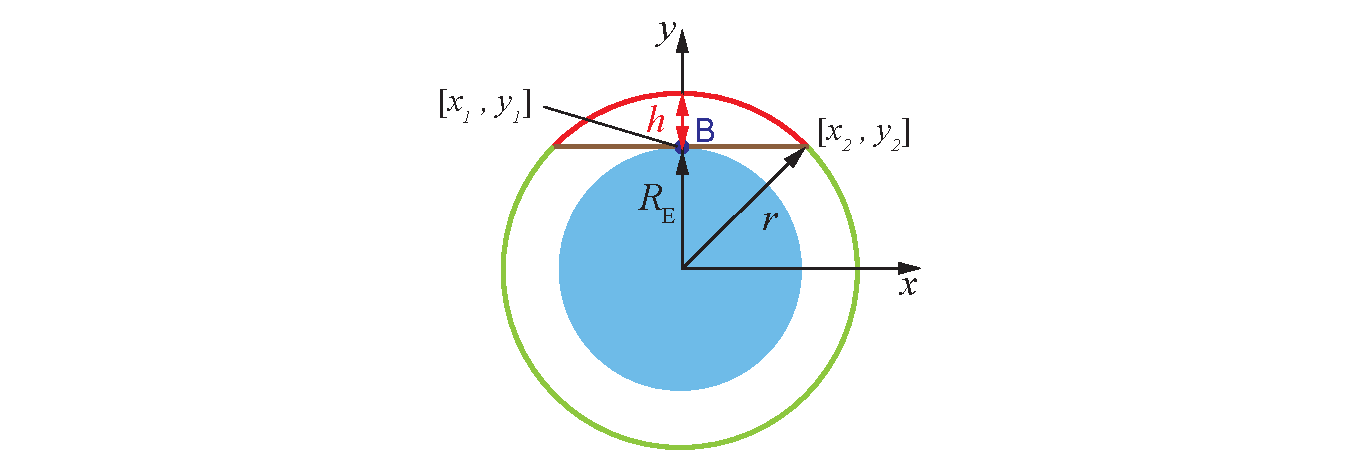
\includegraphics[width=\textwidth]{StarlinkGeometrie.pdf} 
	\caption[Zur Geometrie der Starlink-Beobachtungen.]{[Zur Geometrie der Starlink-Beobachtungen. Mit rot ist die Kugelkappe dargestellt die ein Beobachter auf der Erde sieht, wenn sich ein Starlink-Satellit in einer Kugelschale mit Radius $R_\text{E} + h$ bewegt.}
	\label{abb:adyn_starlink_ueb01}
\end{figure}
\begin{enumerate}
\item [1)] Wir berechnen zun�chst den Anteil $\gamma\lk h\rk$ der Kugelschale mit Radius $R_\text{E} + h$, den ein Beobachter von der Erdoberfl�che aus sieht. \\
    Nach \figref{adyn_starlink_ueb01} ist das:
    \begin{align*}
        \gamma\lk h\rk = \frac{A_\text{KK}}{A_\text{K}} \,. 
    \end{align*}
    Hierin ist $A_\text{K}$ ist die Oberfl�che einer Kugel $4\pi\,r^2 = 4\pi\,\lk R_\text{E} +h\rk^2$ und $A_\text{KK}$ die Oberfl�che der Kugelkappe, die man sich leicht �ber 
    \begin{align*}
       A_\text{KK} &= 2\pi\,r\int\limits_{x_1}^{x_2} y(x)\,\sqrt{1+y'(x){}^2}\D x = 2\pi\int\limits_{\rho_1}^{\rho_2} y(\rho)\,\sqrt{1+y'(\rho){}^2}\,\D \rho 
    \end{align*}
    mit $y = \sqrt{r^2-x^2}$,\,  $1+y'{}^2 = r^2/(r^2-x^2)$,\, $r = R_\text{E} + h$\, und \,$x= \rho\,\cos\phi$ herleiten kann.\\
		Somit erh�lt man 
    \begin{align}
		  A_\text{KK} &= 2\pi\,r \int\limits_{R_\text{E}}^{R_\text{E} + h}\,\D \rho = 2\pi\,\lk R_\text{E} +h\rk \,h \nonumber \\
      \rightarrow~~~  \gamma\lk h\rk &= \frac{2\pi\,\killA{\lk R_\text{E} + h\rk}\,h}{4\pi\,\lk R_\text{E} + h\rk^\killA{2}} = \frac{1}{2}\,\frac{h}{R_\text{E} + h} \,. \label{eq:adyn_starlink_ueb01}
    \end{align}
    Mit den Angaben aus der Aufgabenstellung sind damit jederzeit pro Schale $n_i $ Satelliten 
    \begin{align*}
        n_i = \gamma\lk n_i\rk \cdot \,N_i = 
        \begin{cases} 
        190 \\ 
        63\\
        223
        \end{cases}
    \end{align*}
    und insgesamt $n_\text{ges} = \sum n_i \approx 476$ Satelliten zu sehen.
\newpage
\item [2)] Wir nehmen eine Gleichverteilung der Satelliten in der Kugelschale an. Dann ergibt sich f�r einen Beobachter eine Raumwinkeldichte von
    \begin{align}
        \Omega_\text{ges} = \frac{n_\text{ges}}{2 \pi} \approx 75.8 \,. \label{eq:adyn_starlink_ueb03}
    \end{align}
    Der Nenner von $2\pi$ (anstelle $4\pi$) ergibt sich, aus der Tatsache, dass wir bereits in der Berechnung von \eqref{eq:adyn_starlink_ueb01} ber�cksichtigt hatten, dass der Beobachter nur den Halbraum sieht. Wir rechnen den Raumwinkel auf Quadratgrad ($\square^\degree$) um:
    \begin{align*}
        4\pi^2 = \lk 2\pi\rk^2 \widehat{=} \lk 360^\degree\rk^2 = 129600\,\square^\degree \,.
    \end{align*}
    und erhalten damit aus \eqref{eq:adyn_starlink_ueb03}
    \begin{align}
        \Omega_\text{ges} = \frac{n_\text{ges}}{2\pi} \approx 0.023\,\frac{1}{\square^\degree} \,.\label{eq:adyn_starlink_ueb04}
    \end{align}
    Umgekehrt hei�t das, dass f�r eine Kantenl�nge $d_\square$ eines Winkelquadrats am Himmel von 
    \begin{align}
        d_\square = \sqrt{A_\square} = \frac{1}{\sqrt{\Omega_\text{ges}}} \approx 6.6\degree   \label{eq:adyn_starlink_ueb05}
    \end{align}
    in etwa ein Starlink-Satellit zu sehen ist. \\
    Die Winkelgeschwindigkeit eines Starlink-Satelliten ist nach dem Keplerschen Gesetz durch
    \begin{align*}
        \omega_i = \sqrt{\frac{G\,M_\text{E}}{\lk R_\text{E} +h_i\rk^3}} = 
        \begin{cases} 
        \SI{3.95}{\degree\per\minute} \\ 
        \SI{3.75}{\degree\per\minute}\\
        \SI{3.3}{\degree\per\minute}
        \end{cases} \,.
    \end{align*}
    Der Mond hat einen Winkeldurchmesser von \ca $\SI{0.5}{\degree}$, \dh ein Starlink-Satellit \anf{durchquert} den Mond in weniger als $\Delta t = 0.5/\omega_i \approx \SI{8}{\second}$.
\end{enumerate}

\end{sol} 
\textcolor{blue} {$\rightarrow$ zur} \probref{adyn_orbits5}.\\
\noindent\rule[1ex]{\textwidth}{0.5pt}  \newpage  \clearpage





%-----------------------------------------------------------------------------------------------------------


\subsection{�bungen zu Man�vern im Weltall}

\medskip

%-----------------------------------------------------------------------------------------------------------

\begin{sol}{prob:adyn_rocket_analogy}\label{lsg:adyn_rocket_analogy} %�bung11
\textbf{Analogie zum Oberth-Effekt\index{Oberth-Effekt}}\\

Zun�chst k�nnte man denken, es spielt keine Rolle, wo die Rakete gez�ndet wird. Dem ist aber nicht so.\\
Wir betrachten den Gewinn an kinetischer Energie des Raketenautos durch den kurzen Raketenimpuls ($m_0$ ist die Masse der Rakete ohne Treibstoff) im festen KOS $\sum$:
\begin{align}
\begin{split}
    \Delta T_\text{R} &=\frac{1}{2}\,m_0\,\lk v+\Delta v\rk^2 - \frac{1}{2}\,m_0\,v^2\\
    &= \frac{1}{2}\,m_0\,\lk\Delta v\rk^2 - m_0\,v\,\Delta v  \,. 
\end{split}\label{eq:adyn_rocket_analogy01}
\end{align}
Der Gewinn an kinetischer Energie h�ngt interessanterweise von $v$ ab.\\
Der Impuls der gez�ndeten Rakete auf das Raketenauto ist aber unabh�ngig von $v$:
\begin{align}
    m_0\,\Delta v = m_\text{G}\,v_\text{G} = F\,\Delta t\,, \label{eq:adyn_rocket_analogy02}
\end{align}
worin $m_\text{G}$, $v_\text{G}$ die Masse \bzw die Geschwindigkeit des ausgesto�enen Treibgases sind, $F$ der Schub und $\Delta t$ ein kleines Zeitintervall. \\
Die Bezeichnung Ausstr�mgeschwindigkeit des Treibgases verdient eine genauere Betrachtung, es ist n�mlich die Geschwindigkeit des Gases relativ gemessen zum Schwerpunkt des Systems Raketenauto und Treibstoff. \\
Wie kann man das Paradoxon erkl�ren? Indem man die Ver�nderung der kinetischen Energie des Treibstoffs (\bzw der ausstr�menden Gase) wiederum im festen KOS $\sum$ betrachtet: 
\begin{align}
\begin{split}
    \Delta T_\text{G} &=\frac{1}{2}\,m_\text{G}\,\lk v_\text{G}-v\rk^2 - \frac{1}{2}\,m_\text{G}\,v^2\\
    &= \frac{1}{2}\,m_\text{G}\,v_\text{G}{}^2 - m_\text{G}\,v_\text{G}\,\Delta v \,.
\end{split} \label{eq:adyn_rocket_analogy03}
\end{align}
Man betrachte, dass hier in die Beziehung die Relativgeschwindigkeit $|v_\text{G} - v|$ eingeht, da im festen KOS sich ja der Treibstoff vor dem Z�nden bereits mit $v$ bewegt (\figref{adyn_rocket_analogy02}).\\

\begin{figure}[H]
	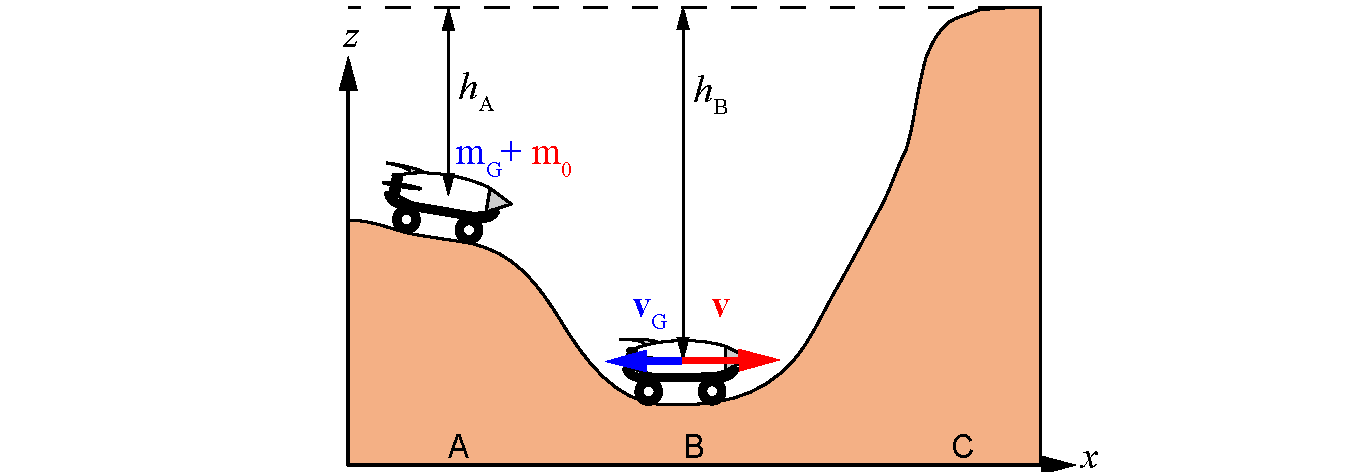
\includegraphics[width=\textwidth]{OberthEffAnalogie.pdf} 
	\caption[Analogie-Modell zum Oberth-Effekt.]{Analogie-Modell zum Oberth-Effekt.}
	\label{abb:adyn_rocket_analogy02}
\end{figure}

Die gesamte Ver�nderung der kinetischen Energie vom Raketenauto und Treibstoff muss gleich der freigesetzten chemischen Energie des Treibstoffs $\Delta E_\text{T}$ sein:
\begin{align}
\begin{split}
    \Delta T &= \Delta T_\text{R} + \Delta T_\text{G} \\
    &=\frac{1}{2}\,m_\text{G}\,v_\text{G}{}^2 + \frac{1}{2}\,m_0\lk\Delta v\rk^2 + \underbrace{m_0\,v\,\Delta v - m_\text{G}\,v\,v_\text{G}}_{\text{wegen \eqref{eq:adyn_rocket_analogy02}} =0} \\
    \Delta T &= \frac{1}{2}\,m_\text{G}\,v_\text{G}{}^2 + \frac{1}{2}\,m_0\lk\Delta v\rk^2 = \Delta E_\text{T}\,. 
\end{split} \label{eq:adyn_rocket_analogy04}
\end{align}
Die gesamte kinetische Energie ist wie erwartet unabh�ngig von $v$ und wegen der Energieerhaltung gleich $\Delta E_\text{T}$. \\

Was bedeutet das nun f�r den Z�ndungszeitpunkt? Wir untersuchen zwei Zeitpunkte (\bzw Orte) $A$ und $B$. 
Es gilt f�r die Gesamtenergien vor dem Z�nden:
\begin{align*}
    E_\text{A} &= -\lk m_0+ m_\text{G}\rk\,g\,h_\text{A}  \,,\\
    E_\text{B} &= -\lk m_0 + m_\text{G} \rk\,g\,h_\text{B} + T_\text{B} \\
    &= -\lk m_0+m_\text{G}\rk\,g\,h_\text{B}  + \frac{1}{2}\lk m_\text{G} +m_0\rk\,v_\text{B}{}^2 = -\lk m_0 + m_\text{G} \rk\,g\,h_\text{A}     \,.
\end{align*}
Aus $E_\text{A} = E_\text{B}$ folgt $v_\text{B} = \sqrt{2g\lk h_\text{B} -h_\text{A}\rk }$.\\

Unmittelbar nach dem Z�nden am Punkt $B$ gilt:
\begin{align*}
    E_\text{R}' =\,&\frac{1}{2}\,m_0\lk v_\text{B}+\Delta v\rk^2 - m_0\,g\,h_\text{B} + \frac{1}{2}\,m_\text{G}\lk v_\text{B} -v_\text{G}\rk^2 - m_\text{G}\,g\,h_\text{B}\\
    = \,&\frac{1}{2}\,m_0\lk\Delta v\rk^2 + m_0\,g\,h_\text{A} -m_0\,\Delta v\,\sqrt{2g\lk h_\text{B}-h_\text{A}\rk} \,,\\
		E_\text{G}' = \,& \frac{1}{2}\,m_\text{G}\,v_\text{G}{}^2 -m_\text{G}\,g\,h_\text{A} - m_\text{G}\,v_\text{G}\,\sqrt{2g\lk h_\text{B}-h_\text{A}\rk} \,,\\
    E_\text{ges}' = \,&\frac{1}{2}\,m_0\,\lk\Delta v\rk^2 + \frac{1}{2}\,m_\text{G}\,v_\text{G}{}^2 - \lk m_0 + m_\text{G}\rk\,g\,h_\text{A} = \, E_\text{A} + \Delta E_\text{T} \,.
\end{align*}
Man erkennt, dass die Energie der Rakete einen von $\sqrt{\lk h_\text{B} -h_\text{A}\rk}$ abh�ngigen Term hat, der offensichtlich verschwindet, wenn $h_\text{B} = h_\text{A}$ ist, es also keine Potentialmulde gibt. \\
Wir bestimmen jetzt noch wie gro� $\Delta v$ sein mu�, um den Punkt C zu erreichen, wenn die Rakete bei $B$ gez�ndet wird. 
\begin{align}
\begin{split}
    \frac{1}{2}\,m_0\,v_\text{C}{}^2 &= \frac{1}{2}\,m_0\,\lk \Delta v\rk^2 - m_0\,g\,h_\text{A} +m_0\,\Delta v \,\sqrt{2g\lk h_\text{B}-h_\text{A}\rk}\\
    \rightarrow ~~~~ 0 &= \lk \Delta v\rk^2 + 2\,\Delta v\,\sqrt{2g\lk h_\text{B}-h_\text{A}\rk} - 2\,g\,h_\text{A}\\
    \rightarrow ~~~~ \lk \Delta v\rk_\text{min} &= \sqrt{2g\lk h_\text{B}-h_\text{A}\rk} + \sqrt{\frac{g}{2}\,\lk h_\text{B}-h_\text{A}\rk + 2\,g\,h_\text{A}} 
\end{split}\,.\label{eq:adyn_rocket_analogy06}
\end{align}
Wie erwartet wird $\Delta v$ f�r $h_\text{B} = h_\text{A}$ zu $\Delta v= \sqrt{2\,g\,h_\text{A}}$. \\
Wir haben $\Delta v\lk h_\text{B}, h_\text{A}\rk$ in \figref{adyn_rocket_analogy03} dargestellt.\\

Die Analogie zum Oberth-Effekt der Raumfahrt ist offensichtlich. Wenn man den gr��tm�glichen beschleunigenden Effekt auf ein Raumschiff haben will, startet man das Man�ver am Punkt der Bahn, wo die Geschwindigkeit am gr��ten ist, \dh im Perig�um oder allgemein an der Periapsis. \\
Einfach gesprochen besagt der Oberth-Effekt, dass ein Raumschiff bei einem Impulsman�ver etwas Energie zus�tzlich zur chemischen Energie des Treibstoffs  \anf{stehlen} kann und zwar von der urspr�nglichen kinetischen Energie, die der Treibstoff vor dem Z�nden auf Grund der Bewegung der Rakete hatte. Anders gesagt: Der Schub generiert einen Impuls proportional zu $\Delta v$. Da die Energie proportional zu $v^2$ ist, ist dieser generierte Impuls energetisch um so wirksamer, je gr��er die Geschwindigkeit $v$ zu Beginn des Schubs ist.


\begin{figure}[H]
	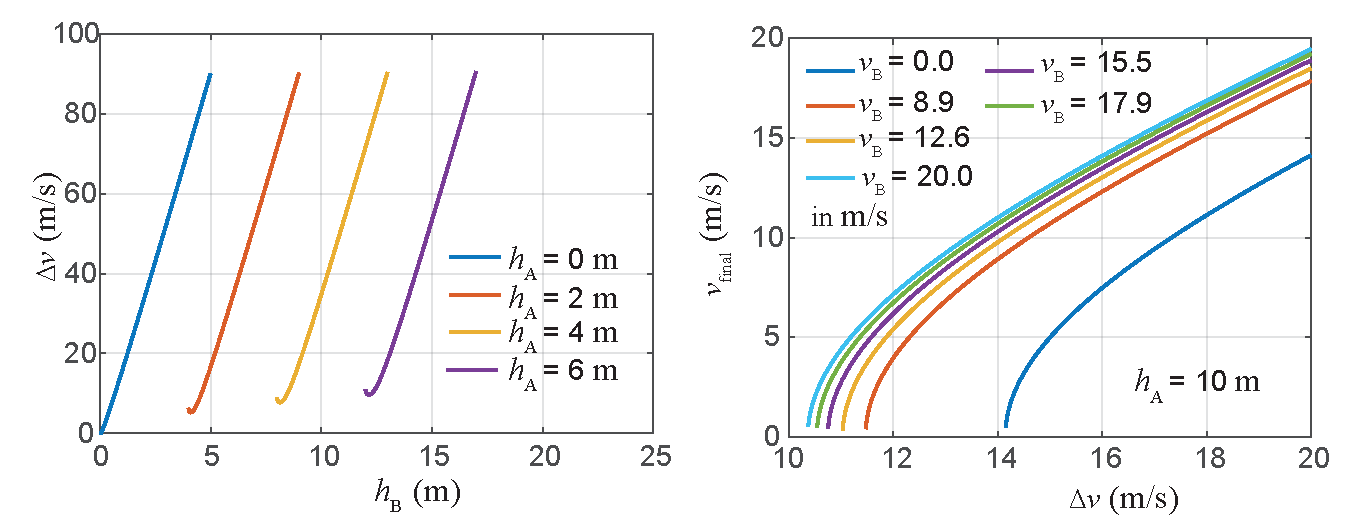
\includegraphics[width=\textwidth]{OberthEffAnalogie02.pdf} 
	\caption[Antriebsbedarf eines Raketenautos durch eine Potentialmulde.]{Antriebsbedarf eines Raketenautos durch eine Potentialmulde als Analogie-Modell zum Oberth-Effekt (Parameter siehe \mscr~\mladynref{OberthEffektAnalogie.m}).}
	\label{abb:adyn_rocket_analogy03}
\end{figure}

\end{sol} 
\textcolor{blue} {$\rightarrow$ zur} \probref{adyn_rocket_analogy}.\\
\noindent\rule[1ex]{\textwidth}{0.5pt}  \newpage  \clearpage


%-----------------------------------------------------------------------------------------------------------

\begin{sol}{prob:adyn_manoevers1}\label{lsg:adyn_manoevers1} %�bung12
\textbf{Hohmann-Transfer}
\begin{itemize}
   \item �bergangszeit f�r den Hohmann-Transfer als Funktion von $r_2/r_1$ \\
	Die �bergangszeit ergibt sich als halbe Umlaufzeit f�r die Hohmann-Ellipse:
	\begin{align*}
    t_\text{H} = \pi\sqrt{\frac{a_\text{H}{}^3}{m_\text{ZK}\,G}} = \frac{\pi}{\sqrt{m_\text{ZK}\,G}}\,\sqrt{\lk \frac{r_1+r_2}{2}\rk^3}\,.
\end{align*}
F�r den Fall eines Hohmann-Transfers von der Erdbahn in den interplanetaren Raum sind die Zeiten in \figref{adyn_Hohmann_TOF} dargestellt (\mscr~\mladynref{HohmannTransfer.m}).
\begin{figure}[H]
	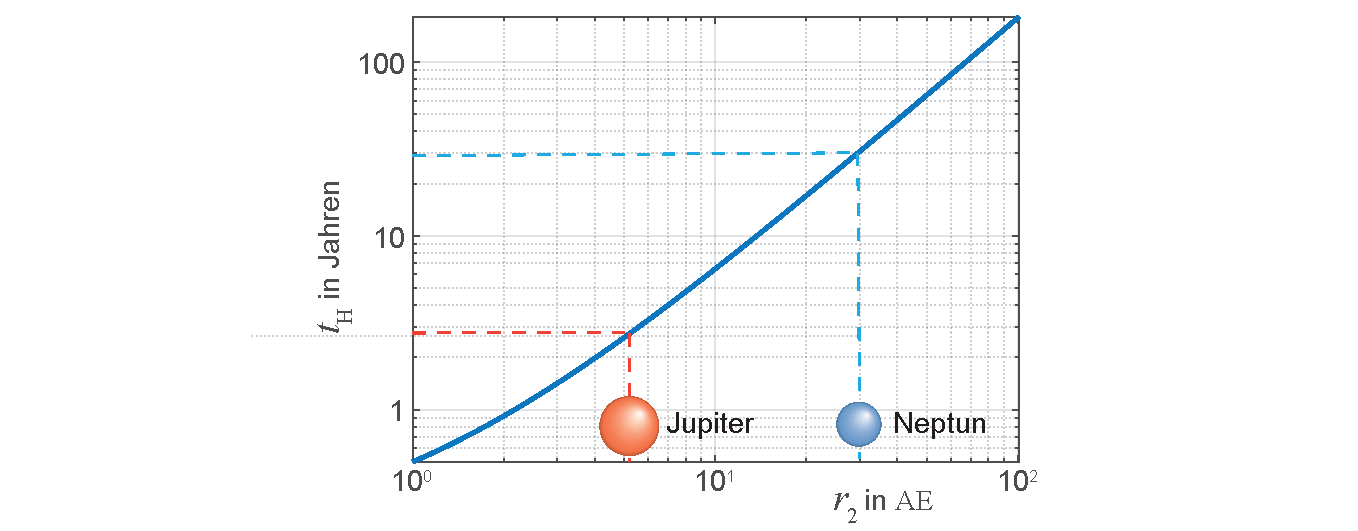
\includegraphics[width=\textwidth]{HohmannTOF.pdf} 
	\caption[Hohmann-Transferzeiten.]{Hohmann-Transferzeiten.}
	\label{abb:adyn_Hohmann_TOF}
\end{figure}
   \item $\Delta v$ gr��er als die \gls{vescape}\\
	F�r $r_2 \rightarrow \infty$ geht $\Delta v_2 \rightarrow 0$ und $\Delta v_1 \rightarrow v_\text{F}$. Daher ist in einem Bereich von $3.3 < r_2/r_1 < \infty$ die Summe $\Delta v_1+\Delta v_2$ gr��er als $v_\text{F}$, wie man leicht aus \eqref{eq:adyn_hohmann04} zusammen mit \eqref{eq:adyn_hohmann03a} und  \eqref{eq:adyn_hohmann03b} herleiten kann.\\
	Im Allgemeinen braucht man insgesamt mehr Antriebsenergie wenn eine Raumsonde erst impulsiv beschleunigt wird, dann durch Gravitation verlangsamt wird und anschlie�end wieder beschleunigt wird, als wenn die gesamte Antriebsimpuls in der Form von $\Delta v_1 = v_\text{F}$ aufgebracht wird.\\
   \item Hohmann-Transfer f�r Verringerung des Bahnradius\\
	Beim Hohmann-�bergang von h�heren auf niedrigere Bahnen gelten die Formeln unver�ndert, der Antriebsbedarf ist negativ und als Schub gegen die Flugrichtung zu verstehen.\\
\end{itemize}

\end{sol} 
\textcolor{blue} {$\rightarrow$ zur} \probref{adyn_manoevers1}.\\
\noindent\rule[1ex]{\textwidth}{0.5pt}  \newpage  \clearpage

%-----------------------------------------------------------------------------------------------------------
\begin{sol}{prob:adyn_manoevers2}\label{lsg:adyn_manoevers2} %�bung13
\textbf{Bielliptischer �bergang}\\

Zwei-Impuls-�bergang von Bahn mit Radius $r_1$ auf eine elliptische Bahn mit Radius $r_2$: 
F�r den Hohmann-Transfer nach $\infty$ ($r_2 \to\infty)$ k�nnen wir schreiben:
\begin{align*}
    \Delta v_1 = \sqrt{\frac{\mu}{r_1}}\,\lk \sqrt{2}-1\rk = v_1\lk \sqrt{2}-1\rk\,.
\end{align*}
Hierin ist $\mu$ der Gravitationsparameter f�r den jeweiligen betrachteten Zentrlk�rper (Erde, Sonne). Analog folgt in der umgekehrten Richtung (aus dem $\infty$ auf die Kreisbahn $r_2$):
\begin{align*}
    \Delta v_2 = v_2 \lk \sqrt{2}-1 \rk
\end{align*}
und somit mit $ \gamma = r_2 / r_1$:
\begin{align*}
    \frac{\Delta v_2}{v_1} = \frac{v_2}{v_1}\,\lk \sqrt{2}-1\rk = \sqrt{\frac{r_1}{r_2}} \,\lk\sqrt{2}-1\rk = \frac{\sqrt{2}-1}{\sqrt{\gamma}}\,.
\end{align*}
Der Gesamt-Antriebsbedarf ist dann: 
\begin{align*}
    \frac{\Delta v}{v_1} = \frac{\Delta v_1+\Delta v_2}{v_1} = \frac{\Delta v_1}{v_1}+\frac{\Delta v_2}{v_1} = \lk \sqrt{2} -1\rk\lk 1 + \frac{1}{\sqrt{\gamma}}\rk\,.
\end{align*}
\begin{figure}[H]
	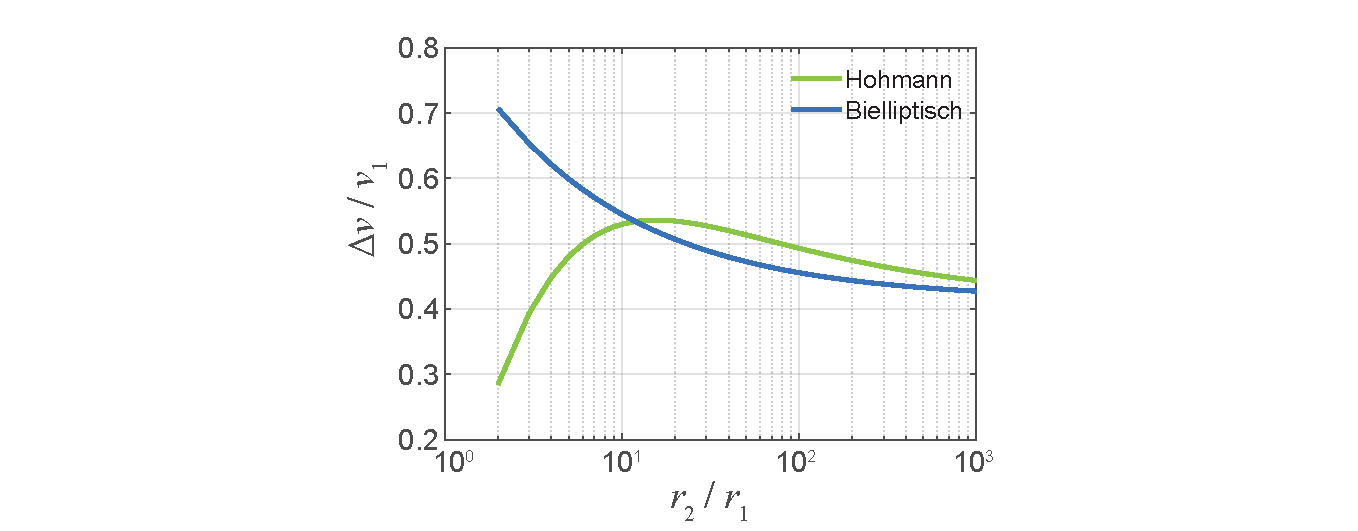
\includegraphics[width=\textwidth]{BiEllptischerTransfer.pdf} 
	\caption[Bielliptischer Transfer.]{Antriebsbedarf beim bielliptischen Transfer im Vergleich zum Hohmann-Transfer.}
	\label{abb:adyn_manoevers2}
\end{figure}

Man erkennt aus \figref{adyn_manoevers2}, dass in der Tat f�r gro�e Radienverh�ltnisse ($\gamma > \SI{11.94}{}$) der bielliptische-Transfer energetisch g�nstiger ist.\\
Allerdings erkauft man sich das durch sehr lange Transferzeiten. Vorteilhaft sind solche bielliptischen �berg�nge aber, wenn man die Inklination und Umlaufrichtung des Orbits �ndern will. Die Rechnungen sind im Detail im \mscr~\mladynref{BiElliptischerTransfer.m} ausgef�hrt.
Die in der Abbildung gezeigten Trajektorien der hyperbolischen Bahnen sind nach \kap{hm_bewegungsgl} gegeben durch:
\begin{align}
	 r = \frac{a\,\lk 1 - e^2 \rk}{1 - e\,\cos\upsilon} ~~~\text{mit}~~~\upsilon < \arccos\frac{1}{e} ~~~\text{und}~~~a = \frac{r_\text{P}}{(1-e)} \,.	\label{eq:adyn_oberth37}
\end{align}
Die geometrischen Parameter $a$ und $e$ der Hyperbel sind durch die physikalischen Parameter $H$ \bzw $v_\infty$ und $r_\text{P}$ definiert (vgl. \kap{hm_bewegungsgl}: $~a < 0,\, e > 1$):
\begin{align}
	 a = -\frac{\mu}{2H_\infty} = -\frac{\mu}{v_\infty{}^2} ~~~\text{und}~~~e = 1 + \frac{r_\text{P}\,v_\infty{}^2}{\mu} \,.	\label{eq:adyn_oberth38}
\end{align}

\end{sol} 
\textcolor{blue} {$\rightarrow$ zur} \probref{adyn_manoevers2}.\\
\noindent\rule[1ex]{\textwidth}{0.5pt}  \newpage  \clearpage

%-----------------------------------------------------------------------------------------------------------

\begin{sol}{prob:adyn_manoevers3}\label{lsg:adyn_manoevers3} %�bung14
\textbf{Hohmann-Oberth-Edelbaum-Transfers aus dem Orbit nach $\infty$}\\

Die Rechnungen sind explizit im \mscr~\mladynref{TransferUnendlich.m} hinterlegt und die Ergebnisse in \figref{adyn_Oberth_transfer2} und \figref{adyn_Oberth_transfer3} gezeigt. 
Man erkennt, dass es f�r gr��ere finale Abst�nde $r_\text{end}$ und bestimmte Verh�ltnisse von $r_{+}/r_1$  ein Minimum der Flugzeit f�r den Edelbaum-Transfer gibt. Er ist in den meisten F�llen der energetisch g�nstigste Transfer. Der Hohmann-Transfer ist f�r gro�e Entfernungen sowohl was die Flugzeit als auch den Antriebsbedarf betrifft der ung�nstigste.\\

\begin{figure}
	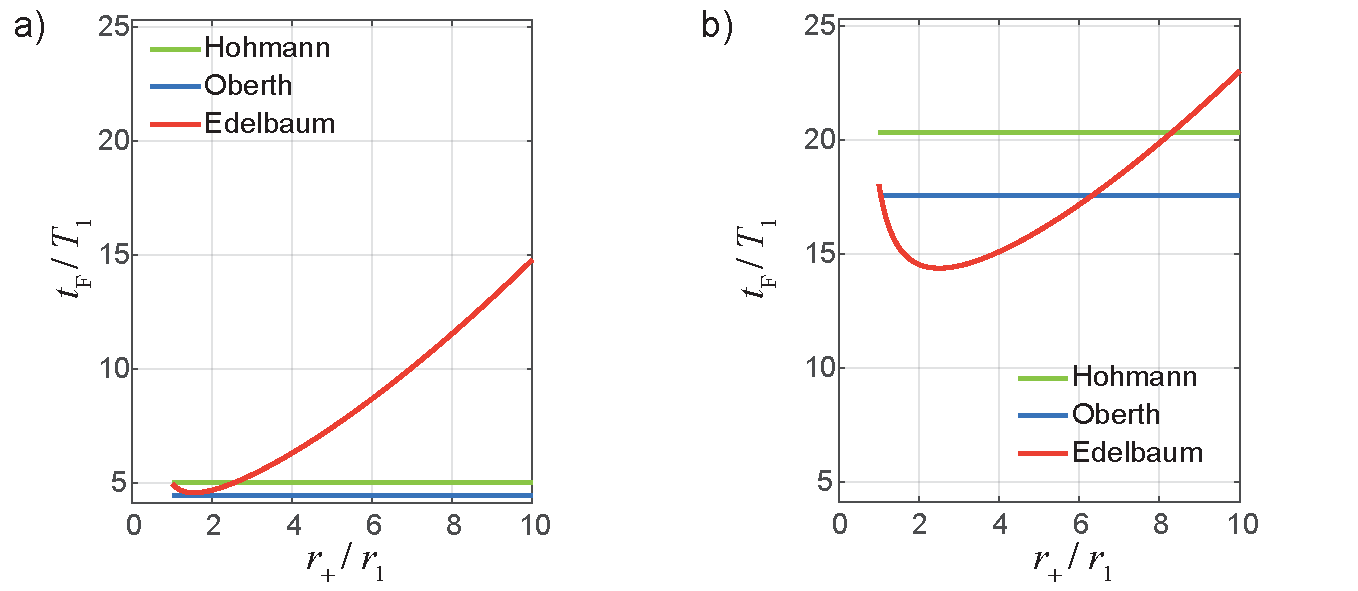
\includegraphics[width=\textwidth]{TransfersInfin03.pdf} 
	\caption[Flugzeiten beim Transfer nach $\infty$.]{Flugzeiten beim Hohmann-, Oberth- \bzw Edelbaum-Transfer. \fa bis zu $r_\text{end}=50\,r_1$ \fb bis zu $r_\text{end}=200\,r_1$.  Als variabler Parameter wurde der �u�ere Radius $r_{+}$ genommen, der innere Radius wurde als fix mit $r_{-}=0.05\,r_1$ gesetzt und der Schubparameter wurde mit $\Delta v/v1 = 1.1$ angenommen. Man erkennt, dass es f�r $r_{+}\approx 2.5\,r_1$ ein absolutes Minimum der Flugzeit f�r den Edelbaum-Transfer gibt. Danach f�hrt die l�ngere Flugzeit auf der Halbellipse von $r_{+}$ nach $r_{-}$ zu insgesamt l�ngeren Flugzeiten.} \label{abb:adyn_Oberth_transfer3}
\end{figure}

\end{sol} 
\textcolor{blue} {$\rightarrow$ zur} \probref{adyn_manoevers3}.\\
\noindent\rule[1ex]{\textwidth}{0.5pt}  \newpage  \clearpage

%-----------------------------------------------------------------------------------------------------------

\begin{sol}{prob:adyn_manoevers4}\label{lsg:adyn_manoevers4} %�bung15
\textbf{Lambert-Problem}\\

Die allgemeine Formulierung des Lambert-Problems lautet wie folgt (\figref{adyn_lambert_lsg02a}):\\
Es seien zwei Punkte $\text{P}_1,\, \text{P}_1$ im Raum durch ihre Vektoren $\vec{r}_1$, $\vec{r}_2$ bekannt, ebenso die Zeit $t_\text{F} = t_2-t_1$, die f�r die Bewegung des K�rpers zwischen $\mathrm{P}_1$ und $\mathrm{P}_2$ ben�tigt wird. Gesucht sind f�r die Kepler-Ellipse die Bahnparameter $a$, $e$, $ \upsilon_0$.\footnote{Wir wollen hier nur Ellipsenbahnen betrachten. Man kann das Problem auch f�r Hyperbelbahnen formulieren und l�sen, siehe \ua \cite{Izzo2015, Walter2018}. Im wesentlichen werden dabei die Winkelfunktionen durch die Hyperbelfunktionen ersetzt.}\\

\begin{figure}[H]
	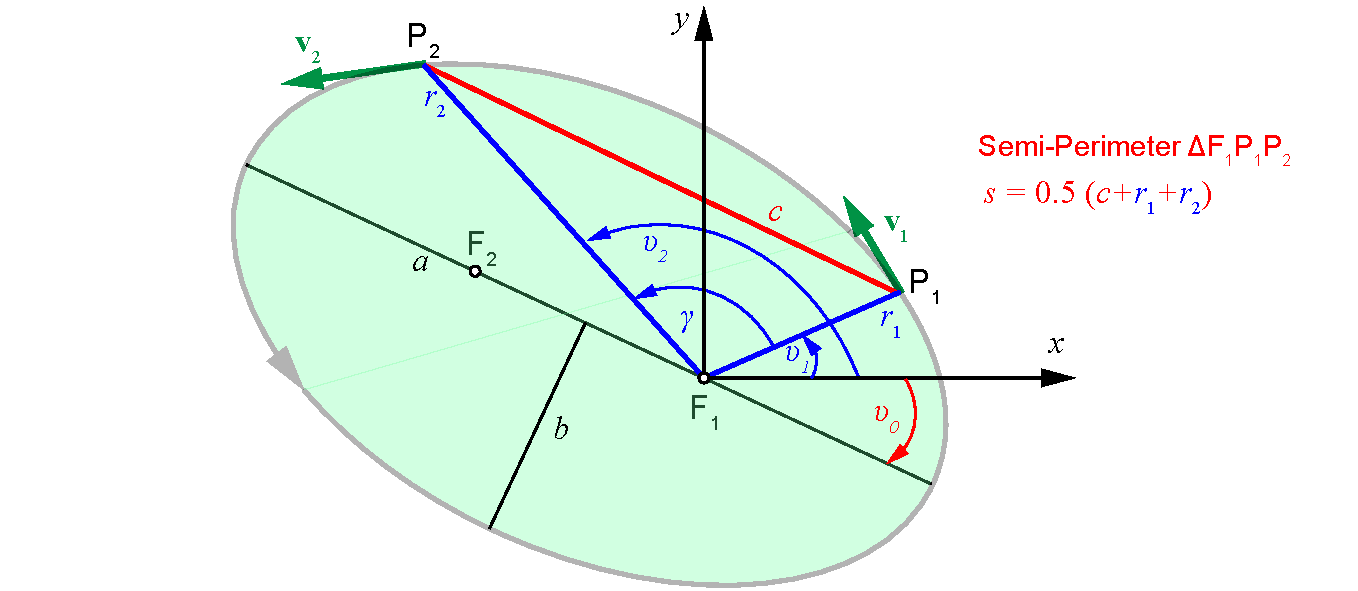
\includegraphics[width=\textwidth]{LambertProblem02Geometrie.pdf} 
	\caption[Geometrie des Lambert-Problems.]{Geometrie des Lambert-Problems. Parameter siehe Text.}
	\label{abb:adyn_lambert_lsg02a}
\end{figure}

Zun�chst schreiben wir die Kepler-Gleichung f�r die beiden Zeitpunkte auf ($\mu$ ist hierin der Gravitationsparameter des Zentralk�rpers, in dessen Schwerefeld die Bewegung stattfindet.) und subtrahieren die beiden Gleichungen voneinander. Wir erhalten:
\begin{align}
\sqrt{\frac{\mu}{a^3}}\,\lk t_2-t_1\rk &= \sqrt{\frac{\mu}{a^3}}\,t_\text{F} = E\lk t_2\rk - E\lk t_1\rk -e\,\lek \sin E\lk t_2\rk -\sin E\lk t_1\rk\rek \nonumber \\
\rightarrow ~~~~ \sqrt{\frac{\mu}{a^3}} \,t_\text{F} &= E_2-E_1 -e\,\lk \sin E_2 -\sin E_1\rk \label{eq:adyn_lsglambert01}\,.
\end{align}
Durch die Randwerte ist ja ein Brennpunkt der Ellipse, n�mlich $\mathrm{F}_1$ bekannt. Man sucht nun den Brennpunkt $\mathrm{F}_2$ (oft auch versteckter Fokus genannt), mit dem dann die Ellipse eindeutig definiert ist und zugleich die Bedingung erf�llt ist, dass f�r das Durchlaufen von $\mathrm{P}_1$ nach $\mathrm{P}_2$ die Zeit $t_\text{F}$, im Englischen auch \gls{ToF} (ToF), ben�tigt wird. 

\begin{figure}[H]
	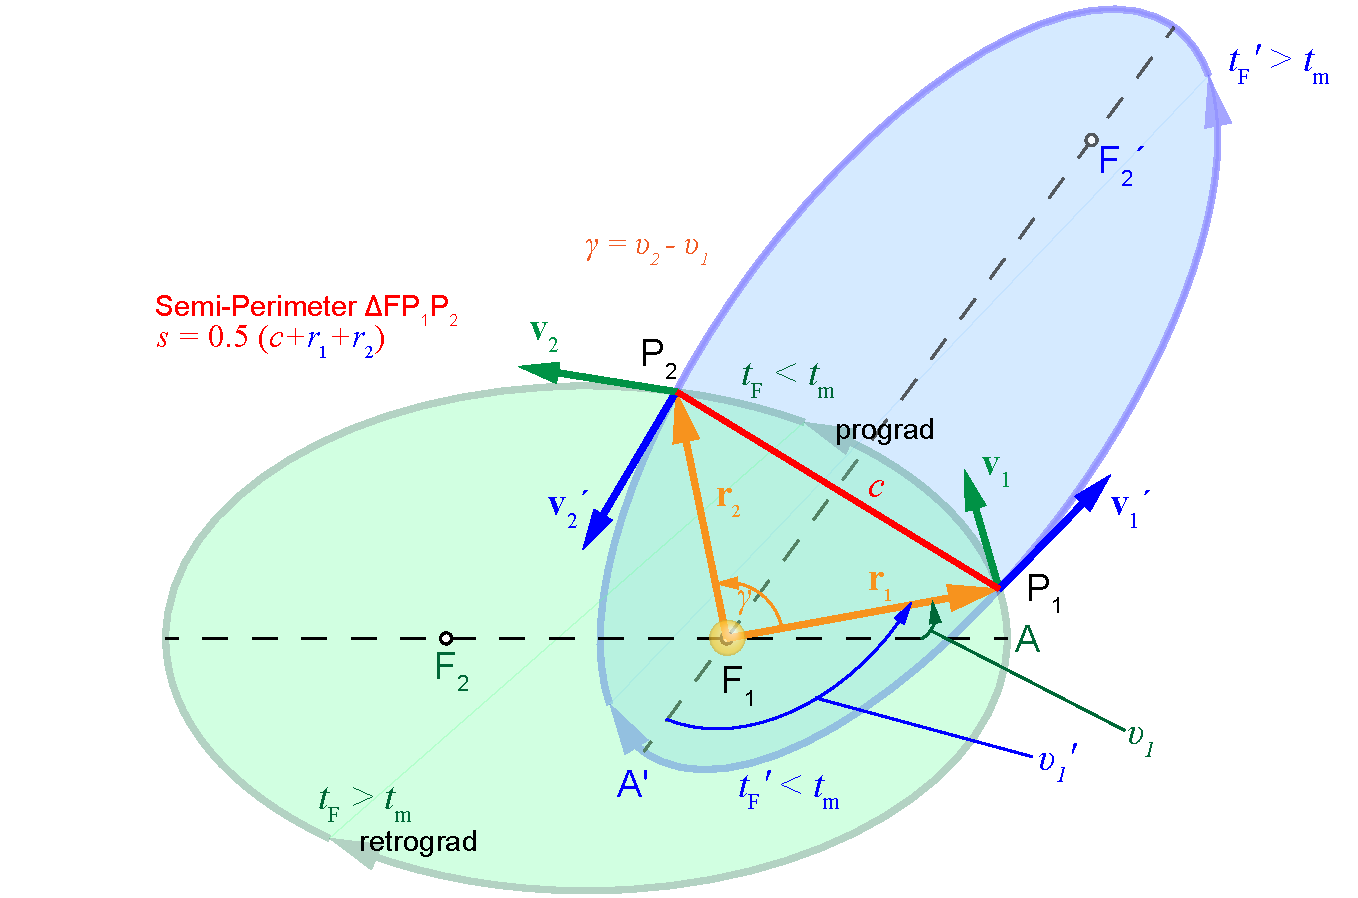
\includegraphics[width=\textwidth]{LambertProblem02Allgemein.pdf} 
	\caption[Geometrie des Lambert-Problems.]{Geometrie des Lambert-Problems. Die beiden Ellipsen (gr�n und blau schattiert) stellen jeweils eine L�sung des Lambert-Problems f�r unterschiedliche Flugzeiten und Flugrichtungen dar. Die Flugrichtung wird als prograd bezeichnet, wenn diese entgegen des Uhrzeigersinns von $\mathrm{P}_1$ nach $\mathrm{P}_2$ erfolgt, die entgegengesetzte Flugrichtung wird retrograd genannt. Die Vektoren $\vec{r}_1$, $\vec{r}_2$ definieren die Ellipsen, sie k�nnen als Positionsvektoren aber auch zu unterschiedlichen Umlaufbahnen geh�ren, \zb $\vec{r}_1$ kann ein Vektor von der Sonne zur Erde sein, $\vec{r}_2$ eine entsprechender Vektor zum Mars. Weitere Parameter siehe Text.}
	\label{abb:adyn_lambert_lsg02}
\end{figure}
Wir k�nnen uns nun leicht �berlegen, dass es f�r die gesuchte Bahn zwei Ellipsen als denkbare L�sungen gibt und zwar mit den beiden "`versteckten"' Fokuspunkten $\mathrm{F}_2$ und $\mathrm{F}_2{}'$ (\figref{adyn_lambert_lsg02})\footnote{Man kann sich die zwei L�sungen anschaulich-geometrisch deutlich machen, in dem man sich die Konstruktionsvorschrift einer Ellipse in Erinnerung ruft. Nach dieser ist an jedem Punkt einer Ellipse die Summe des Abstandes zu den beiden Fokuspunkten konstant und gleich $2a$. Die Konstruktion erfolgt, in dem man einen Kreis um $\mathrm{P}_1$ mit dem Radius $2a-r_1$ schl�gt und einen um $\mathrm{P}_2$ mit $2a-r_2$. Es ergeben sich zwei Schnittpunkte, dies sind die Brennpunkte $\mathrm{F}_2$ \bzw $\mathrm{F}_2{}'$.}.\\
Mit den Beziehung \eqref{eq:hm_r_param_ellipse} und \eqref{eq:hm_bahnglg} aus dem \kap{hm_abl_kepler} k�nnen wir schreiben: 
\begin{subequations}
\begin{align}
    r_{1,2} &= a\,\lk 1-e\,\cos E_{1,2}\rk  \label{eq:adyn_lsglambert02a} \,,\\
    \cos\lk \upsilon_{1,2}-\upsilon_0\rk &= \frac{a}{r_{1,2}}\,\lk\cos E_{1,2}-e\rk \,. \label{eq:adyn_lsglambert02b}
    %r_{1,2}\cos{\upsilon_{1,2}} &= a\,\lk \cos E_{1,2} - e \rk \,, \label{eq:adyn_lsglambert02b} \\
    %r_{1,2}\sin{\upsilon_{1,2}} &= a\,\sqrt{\lk 1-e^2 \rk}\, \sin E_{1,2} \,, \label{eq:adyn_lsglambert02c} \\
\end{align} %\label{eq:adyn_lsglambert02} 
\end{subequations}
Wir betrachten eine der beiden Ellipsen aus \figref{adyn_lambert_lsg02} genauer und verwenden die Darstellung in \figref{adyn_lambert_lsg02a}. Unser Ziel ist es ja, die Trajektorie $r(\upsilon)$ zu finden:
\begin{align}
    r (\upsilon) &= \frac{a\,\lk 1 - e^2 \rk}{1+e\,\cos\lk\upsilon - \upsilon_0 \rk}\,. \label{eq:adyn_lsglambert_traj} 
\end{align} 
In einer Ebene ist eine Trajektorie (Bahn) durch 3 Parameter eindeutig bestimmt. Das Lambert-Problem ist ein planares Problem und wir
haben mit dem Gleichungssystem \eqref{eq:adyn_lsglambert01}, \eqref{eq:adyn_lsglambert02a} und \eqref{eq:adyn_lsglambert02b} ein System f�r 5 Unbekannte $E_1$, $E_2$, $a$, $e$, $\upsilon_0$ mit den bekannten Gr��en $r_1$, $r_2$, $\upsilon_1$, $\upsilon_2$, $t_\text{F}$ und $\mu$.\footnote{Eigentlich sind $\upsilon_1$, $\upsilon_2$ ja nicht bekannt, sondern nur deren Differenz. Durch freie Festlegung eines \KOS wie in \figref{adyn_lambert_lsg02a} gezeigt kann man sich aber $\upsilon_1$ und $\upsilon_2$ berechnen. Man beachte, dass dieses \KOS mit den $x-y$- Achsen in der Ellipsenebene liegt und gegebenenfalls durch Drehung in ein anderes (\zb heliozentrisches) \KOS transformiert werden muss, wenn man die koordinaten der Trajektorie in diesem haben  m�chte.} Dieses System wollen wir jetzt l�sen:
\begin{enumerate}
    \item [1.] Mit der Nebenrechnung (\cite{Gradshteyn1980})
		\begin{align*}
		\sin x - \sin y =&  \sin{\lk \frac{x-y}{2} +  \frac{x+y}{2}\rk} - \sin{\lk \frac{x+y}{2} +  \frac{-x+y}{2}\rk} \\
		=& \sin{\lk \frac{x-y}{2} +  \frac{x+y}{2}\rk} + \sin{\lk \frac{x-y}{2} + \frac{-x-y}{2} \rk} \\
		=& \sin\lk \frac{x-y}{2}\rk\,\cos\lk\frac{x+y}{2}\rk + \sin\lk \frac{x+y}{2}\rk\,\cos\lk\frac{x-y}{2}\rk\\
		&+ \sin\lk \frac{x-y}{2}\rk\,\cos\lk\frac{x+y}{2}\rk - \sin\lk \frac{x+y}{2}\rk\,\cos\lk\frac{x-y}{2}\rk \\
		=& 2\,\sin{\frac{x-y}{2}}\,\cos{\frac{x+y}{2}}
		\end{align*}
    f�hren wir $\psi$ und $\varphi$ als neue Variable ein:
    \begin{align}
        \psi = \frac{E_2-E_1}{2}~~~~ \text{und} ~~~~ \cos \varphi = e\,\cos\lk \frac{E_2 +E_1}{2} \rk \,, \label{eq:adyn_lsglambert06}
    \end{align}
		wobei $\psi \in [0, \pi]$ und $\varphi \in [0, \pi]$ gilt. Wir erhalten dann die Kepler-Gleichung \eqref{eq:adyn_lsglambert01} in folgender vereinfachter Form:
\begin{align}
			\sqrt{\frac{\mu}{a^3}} \,t_\text{F} &= \psi - \cos\varphi\, \sin\psi \label{eq:adyn_lsglambert01a}\,.
\end{align}
Die beiden Gr��en $\psi$ und $\varphi$ h�ngen nur von der vorgegebenen Geometrie des Problems ab, wie man leicht nachrechnen kann, in dem man 
den Abstand von $\mathrm{P}_1$ und $\mathrm{P}_2$ unter Verwendung von \eqref{eq:adyn_lsglambert02b} �ber 
    \begin{align}
        c^2 &= \lk r_2\,\cos\upsilon_2 - r_1\,\cos\upsilon_1 \rk^2 + \lk r_2\,\sin\upsilon_2 - r_1\,\sin\upsilon_1 \rk^2 ~\nonumber \\
				&= r_1{}^2+r_2{}^2 - 2\,r_1\,r_2\,\cos\lk \upsilon_2-\upsilon_1\rk = r_1{}^2+r_2{}^2 - 2\,r_1\,r_2\,\cos\lk \gamma \rk~\nonumber \\
				\rightarrow~~c &= 2 a\,\sin\psi\,\sin\varphi\, \label{eq:adyn_lsglambert03a}
    \end{align}
berechnet. 
Ebenso erh�lt man die Summe der Abst�nde $r_1+r_2$ von den Punkten $\mathrm{P}_1$ und $\mathrm{P}_2$ zum Brennpunkt $\mathrm{F}_1$ wiederum unter Verwendung von \eqref{eq:adyn_lsglambert02b} zu
		\begin{align}
		r_1 + r_2  &= 2a\lk 1- \cos\psi\, \cos\varphi \rk\,. \label{eq:adyn_lsglambert03b}
    \end{align} 
Die Gleichungen \eqref{eq:adyn_lsglambert03a} und \eqref{eq:adyn_lsglambert03b} bestimmen die Gr��en $\psi$ und $\varphi$ eindeutig. Man kann also schlussfolgern, dass die Zeit $t_\text{F}$ nach \eqref{eq:adyn_lsglambert01a} nur eine Funktion von $a$ und den bekannten geometrischen Gr��en $c$ und $r_1 + r_2$  ist.\footnote{Der Beweis daf�r wurde von Lagrange erbracht, der zeigte, dass die ToF $t_\text{F}$ nur von der Energie der Bahn und damit nur von $a$ abh�ngt.}\\   

\item [2.] Um uns die Rechnungen zu erleichtern, f�hren wir zwei weitere Gr��en ein, die wir aus $\varphi$ und $\psi$ wie folgt bilden:
				\begin{align}
						\alpha= \varphi +\psi ~~~~ \text{und} ~~~~ \beta= \varphi-\psi \,. \label{eq:adyn_lsglambert05}
				\end{align}
		Offensichtlich gilt: $\alpha \in [0,\, 2\pi]$ und $\beta \in [-\pi,\, \pi]$. \\
		
\item [3.] Wir bezeichnen den halben Umfang (Semi-Perimeter) des Dreiecks $\Delta \,\mathrm{F}_1\mathrm{P}_1\mathrm{P}_2$ mit 
    \begin{align}
        s= \frac{r_1+r_2+c}{2}\,. \label{eq:adyn_lsglambert04}
    \end{align}
		Damit und mit \eqref{eq:adyn_lsglambert03a} und \eqref{eq:adyn_lsglambert03b} findet man  f�r $\alpha$ die Beziehung: 
    \begin{subequations}
    \begin{align}
        \frac{s}{2a} &= \frac{1}{2} \lek 1 - \cos\psi\cos\varphi + \sin\psi\sin\varphi \rek = \frac{1}{2} \lek 1 - \cos \lk \psi+\varphi \rk \rek \nonumber \\
				&= \frac{1}{2} \lek 1 - \cos\alpha \rek = \frac{1}{2} \lek 1 - \cos\lk \frac{\alpha}{2} + \frac{\alpha}{2} \rk \rek \nonumber \\
				&= \frac{1}{2} \lek 1 - \cos^2\frac{\alpha}{2} + \sin^2\frac{\alpha}{2} \rek = \frac{1}{2} \lek 2\sin^2\frac{\alpha}{2} \rek \nonumber \\
        &\rightarrow~~ \sin^2\lk \frac{\alpha}{2}\rk = \frac{s}{2a}\, \label{eq:adyn_lsglambert06a} \\
				&\text{und entsprechend f�r}~~ \beta \nonumber \\
        &\rightarrow~~ \sin^2\lk\frac{\beta}{2}\rk = \frac{s-c}{2a}\,\label{eq:adyn_lsglambert06b}
    \end{align}
    \end{subequations}
    Sowohl $\alpha$ als auch $\beta$ sind somit Gr��en, die nur von der Geometrie der Aufgabenstellung und dem Bahnparameter $a$ abh�ngen.\\
		
\item [4.] Wir setzen nun \eqref{eq:adyn_lsglambert06a} und \eqref{eq:adyn_lsglambert06b} in \eqref{eq:adyn_lsglambert01} ein und erhalten die elegante Formulierung des Lambert-Problems 
\begin{align}
    t_\text{F} &= \sqrt{\frac{a^3}{\mu}}\,\lk \alpha-\beta-\lek\sin\alpha -\sin\beta\rek\rk\,,\label{eq:adyn_lsglambert07}
\end{align}   
Damit haben wir $E_2$, $E_1$ aus der Kepler-Gleichung eliminiert und das Lambert-Problem auf ein System von 3 Unbekannten ($a$, $\alpha$, $\beta$) zur�ck gef�hrt, von den $\alpha$ und $\beta$ neben den bekannten Gr��en $s$, $c$ nur noch von $a$ abh�ngen. Der Winkel $\alpha$ ist dabei wegen des Quadrats in \eqref{eq:adyn_lsglambert06a} nicht eindeutig bestimmt, es gibt zwei L�sungen
\begin{align}
	\alpha ~~~\text{und}~~~ \alpha'=2\pi-\alpha\,, \label{eq:adyn_lsglambert08}
\end{align}
die den beiden Ellipsenl�sungen und damit auch den beiden Zeit $t_\text{F}$ \bzw $t_\text{F}'$ in \figref{adyn_lambert_lsg02} entsprechen. Der Wert f�r $\beta$ ist hingegen f�r ein aus \eqref{eq:adyn_lsglambert08} folgendes  $a$ \bzw $a'$ eindeutig bestimmt. Man muss aber folgende Fallunterscheidung machen: 
\begin{align}
    \beta = \left\{
\begin{array}{ll}
+2\arcsin\sqrt{(s-c)/a} ~~ & \text{f�r} ~~~~ \gamma = \upsilon_2-\upsilon_1 <\pi \\
-2\arcsin\sqrt{(s-c)/a} ~~ & \text{f�r} ~~~~ \gamma = \upsilon_2-\upsilon_1 >\pi \\
\end{array}
\right.\,.\label{eq:adyn_lsglambert09}
\end{align}

\item [5.] Setzen wir $\alpha\lk a,a' \rk$ und $\beta\lk a,a' \rk$ in \eqref{eq:adyn_lsglambert07} ein, erhalten wir demzufolge zwei Kurven $t_\text{F}\lk a\rk$, die vom Punkt $\lek a_\text{min},\, t_\text{m} \rek$ ausgehen (siehe \figref{adyn_lambert_lsg03}). Hierbei ist $a_\text{min} = s/2$, wie man leicht nachpr�fen kann. Die Ellipse, die durch $a_\text{min}$ definiert wird auch Minimal-Energie-Bahn genannt, wegen $E_\text{min}= -\mu/(2a_\text{min})$. Das ist aber nicht zu verwechseln mit dem minimalen Antriebsbedarf $\Delta v_\text{min}$. Ebenso ist $t_\text{m}$ nicht die minimale Flugzeit, sondern die Flugzeit f�r die Bahn mit der kleinsten Bahnenergie. Wie bereits erw�hnt und aus \figref{adyn_lambert_lsg02} zu erkennen, gibt es zu einem bestimmten Wert von $a$ zwei ToF, die dem kurzen ($t_\text{F} < t_\text{m}$) \bzw  der dem langen Transfer ($t_\text{F} > t_\text{m}$) von $\mathrm{P}_1$ nach $\mathrm{P}_2$ entsprechen.\end{enumerate}

Wir wollen nun Gleichung \eqref{eq:adyn_lsglambert07} l�sen. Das ist analytisch nicht m�glich. Da sie aber eine gewisse �hnlichkeit mit der Kepler-Gleichung hat, k�nnen wir �hnliche Iterationsmethoden wie in \kap{iteration_kepler} benutzen. Wir wollen hier das sogenannte Bisektionsverfahren \cite{Arens2008} verwenden. Man geht folgenderma�en vor:
\begin{enumerate}
    %1.
    \item [1.] Wir bestimmenen die Flugzeit f�r eine Parabell�sung von $\text{P}_1$ nach $\text{P}_2$. Diese l�sst sich aus der Barker-Gleichung\index{Barker-Gleichung} \eqref{eq:hm_Barker_glg} bestimmen:\footnote{F�r die interessierten Leser empfehlen wir die Herleitung von \eqref{eq:adyn_lsglambert11} aus der Barker-Gleichung\index{Barker-Gleichung} \eqref{eq:hm_Barker_glg} (siehe  \kap{kometen}) nachzuvollziehen.} % und verweisen auf die Referenzen \cite{Izzo2015}, \cite{Sangra2021}
			\begin{align}
								t_\text{Par} &= \frac{\sqrt{2}}{3}\,\sqrt{\frac{s^3}{\mu}}\,\lk 1-\sqrt{\lk\frac{s-c}{s}\rk^3}\rk\,.\label{eq:adyn_lsglambert11}
			\end{align}
    %2.
    \item [2.] Wir definieren mit \eqref{eq:adyn_lsglambert07} die Funktion\\
			\begin{align}
						\tau\lk a\rk &= \sqrt{\frac{a^3}{\mu}}\,\lek \alpha\lk a\rk -\beta\lk a \rk - \lk \sin\alpha\lk a\rk-\sin\beta\lk a\rk \rk\rek\,.\label{eq:adyn_lsglambert11a}
			\end{align}
    Gesucht ist das $a$, welches $\tau\lk a\rk = t_\text{F}$ erf�llt.
    %3.
    \item [3.] Wir setzen nun $a_\text{min} = s/2$ und bestimmen damit $t_\text{m} = \tau\lk a_\text{min} \rk$. Ist $t_\text{m} > t_\text{F} > t_\text{Par}$,
		so muss eine (elliptische) L�sung existieren.\footnote{F�r $t_\text{F} < t_\text{Par}$ kann man einen hyperbolischen Transfer von $\mathrm{P}_1$ nach $\mathrm{P}_2$ finden, der noch schneller als der parabolische ist. Wir verweisen auf \cite{Izzo2015, Walter2018}.} Ist $t_\text{Par} < t_\text{F} < t_\text{m}$, dann gibt es eine L�sung auf dem unteren Ast in \figref{adyn_lambert_lsg03}, f�r $t_\text{F} > t_\text{m}$ kann es eine L�sung auf dem oberen Ast geben. Man muss das Bisektionsverfahren entsprechend anpassen, siehe dazu auch \mscr~\mladynref{LambertProblem02.m}. 
    %4.
    \item [4.] Wir suchen nun ein $a_\text{max} \gg a_\text{min}$ und setzen $a_1 = (a_\text{min} + a_\text{max})/2$.
    %5.
    \item [5.] Wir bestimmen $\tau\lk a_1\rk$.
    %6.
    \item [6.] Falls $\tau\lk a_1\rk> t_\text{F}$, dann setzen wir $a_2= (a_1+a_\text{max})/2$, falls $\tau\lk a_1\rk <t_\text{F}$, dann setzen wir $a_2 = (a_\text{min}+a_1)/2$.
    %7.
    \item [7.] Wir wiederholen die Schritte bis zur gew�nschten Genauigkeit von $\tau\lk a_n\rk \approx t_\text{F}$. 
\end{enumerate}
Dieses Verfahren konvergiert, falls �berhaupt eine L�sung existiert: deshalb muss man im Schritt 1 �berpr�fen, ob f�r die gegebenen Werte $r_1$, $r_2$, $\gamma$ und $t_\text{F}$ �berhaupt eine elliptische L�sung existiert. 

\begin{figure}[H]
	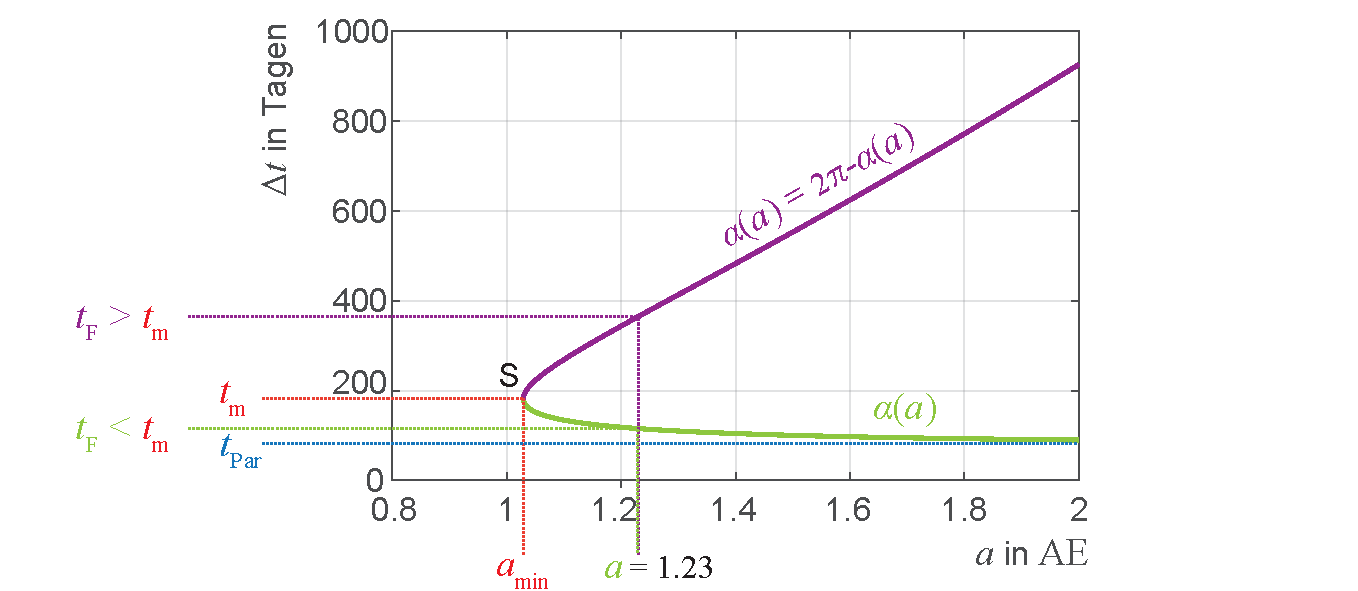
\includegraphics[width=\textwidth]{LambertProblem02Zeiten.pdf} 
	\caption[L�sung des Lambert-Problems.]{L�sung des Lambert-Problems f�r folgende Parameter: $r_1 = \SI{1.0}{AE},\, r_2 = \SI{1.525}{AE},\, \gamma = 75\degree$, und einer ToF von $t_\text{F} = 115 \mathrm{d}$ \bzw $t_\text{F} = 365 \mathrm{d}.$ Siehe \mscr~\mladynref{LambertProblem02.m}.}
	\label{abb:adyn_lambert_lsg03}
\end{figure}
Wir brauchen jetzt noch, nachdem wir $a$ bestimmt haben, die Bahnparameter $e$ und $\upsilon_0$. Aus \eqref{eq:adyn_lsglambert02a} finden wir 
\begin{align}
    E_1 = \arccos \lk \frac{a-r_1}{a\,e} \rk  \label{eq:adyn_lsglambert13}
\end{align}
und aus \eqref{eq:adyn_lsglambert02b} auch $\upsilon_0$
\begin{align}
    \upsilon_0 = \upsilon_1 - 2\,\arctan\lk \sqrt{\frac{1+e}{1-e}}\,\tan\frac{E_1}{2}\rk\,.  \label{eq:adyn_lsglambert14}
\end{align}
Setzen wir das gefundene $a$ in die Gleichungen f�r $\alpha$ und $\beta$ ein und diese wiederum in die f�r $\varphi$ und $\psi$ finden wir mit \eqref{eq:adyn_lsglambert02b} f�r die Exzentrizit�t
\begin{align}
    e = \sqrt{\frac{\lk r_2-r_1\rk^2}{\lk2a\,\sin\psi\rk^2}+\cos^2\varphi}\,.  \label{eq:adyn_lsglambert15}
\end{align}

Hat man mittels Bisektionsverfahren entweder $p$  (mit \mscr~\mladynref{LambertProblem01.m}) oder $a$  (mit \mscr~\mladynref{LambertProblem02.m}) bestimmt, kann man �ber folgende  Beziehung die Geschwindigkeiten an den Punkten $\mathrm{P}_1$ nach $\mathrm{P}_2$ auf der Trajektorie bestimmen (\cite{Walter2018, Battin1999}:
\begin{align}
\begin{split}
    \vec{v}_\text{tr, 1} &= \sqrt{\frac{\mu\,p}{r_1\,r_2\,\sin\gamma}}\,\lek \lk \vec{r}_2 - \vec{r}_1 \rk  + \frac{r_2}{p}\,\lk 1- \cos\gamma \rk\,\vec{r}_1 \rek \\
    \vec{v}_\text{tr, 2} &= \sqrt{\frac{\mu\,p}{r_1\,r_2\,\sin\gamma}}\,\lek \lk \vec{r}_2 - \vec{r}_1 \rk  + \frac{r_1}{p}\,\lk 1- \cos\gamma \rk\,\vec{r}_2 \rek \,.
\end{split}  \label{eq:adyn_lambert16}
\end{align}
Die Richtung der Periapsis (Perihel, Perig�um \usw) und damit der Wert f�r $\upsilon_0$ kann dann �ber den Laplace-Vektor\index{Laplace-Vektor} $\vec{e}$ und \eqref{eq:hm_laplace_int} aus \kap{hm_abl_kepler} wie folgt bestimmt werden:
\begin{align}
    \vec{e} &= \lk \frac{1}{r_1} - \frac{1}{a} \rk \, \vec{r}_1  - \frac{1}{\mu} \, \lk \vec{r}_1 \cdot \vec{v}_\text{tr, 1} \rk \, \vec{v}_\text{tr, 1} \,. 
		\label{eq:adyn_lambert17}
\end{align}

Wir haben das Bisektionsverfahren zur L�sung des Lambert-Problems exemplarisch f�r zwei verschiedene F�lle im \mscr~\mladynref{LambertProblem01.m} \bzw \mscr~\mladynref{LambertProblem02.m} hinterlegt. Fall 1 ist der Transfer einer Raumsonde von der ISS aus $h \approx \SI{422}{\km}$ in die Stratosph�re ($h \approx \SI{22}{\km}$) innerhalb von 50 min und Fall 2 ein Raumflug von der Erde zum Mars f�r eine Flugdauer von 115 Tagen. \figref{adyn_lambert_lsg04} und Tabelle \ref{tab:adyn_bisection} zeigen den Verlauf der Iteration f�r den Fall 2.\\

Im \mscr~\mladynref{LambertProblem03.m} haben wir die Rechnungen mit einer modernen, stabileren numerischen Routine zur L�sung des Lambert-Problems (\cite{Mahooti2015}) wiederholt. Die Routine basiert auf den Ans�tzen, die in \cite{Battin1999, Izzo2015, Walter2018} ausf�hrlich beschrieben sind. Sie beinhaltet auch hyperbolische L�sungen. Die �bereinstimmung mit dem Bisektionsverfahren f�r die angegebenen Beispiele ist sehr gut.

\begin{figure}[H]
	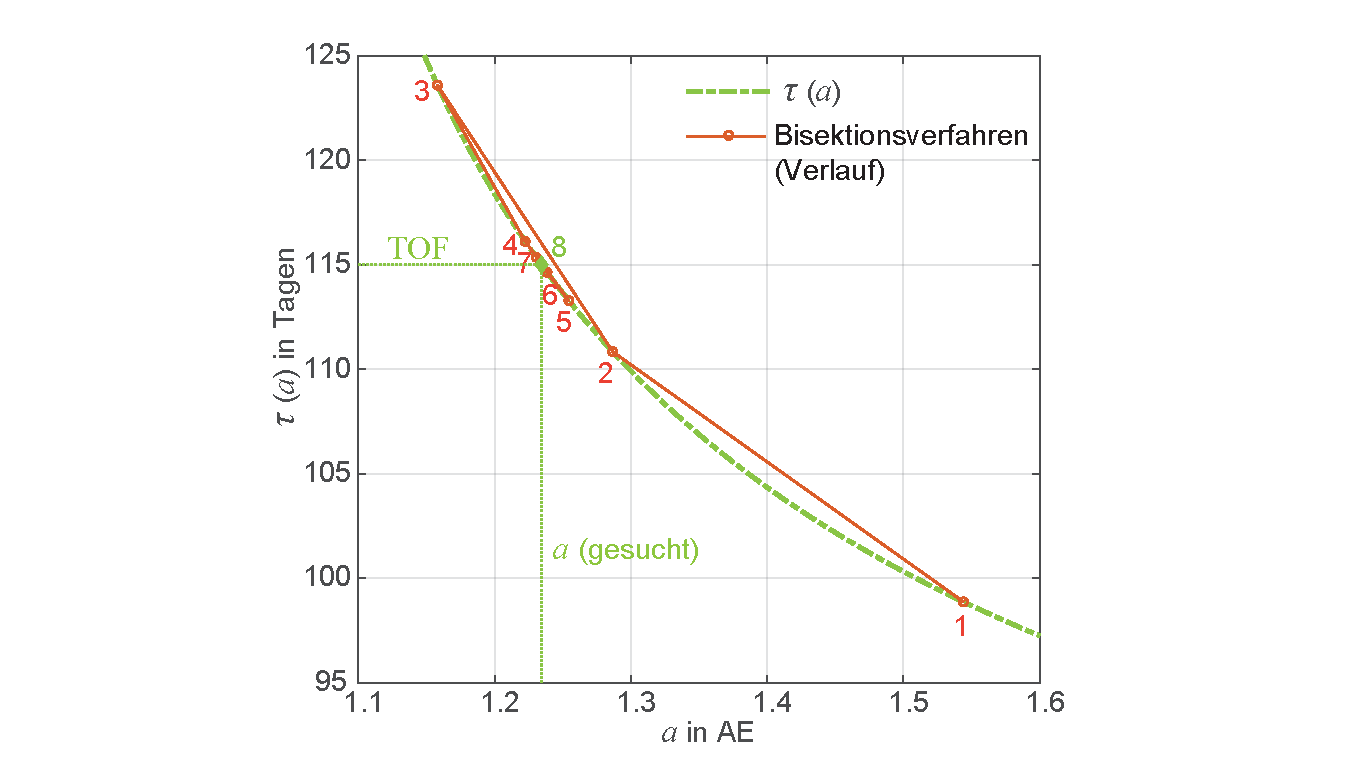
\includegraphics[width=\textwidth]{BisektionLambert.pdf} 
	\caption[Bisektionsverfahren zur L�sung des Lambert-Problems.]{Bisektionsverfahren zur L�sung des Lambert-Problems f�r folgende Parameter: $r_1 = \SI{1.000}{AE},\, r_2 = \SI{1.525}{AE},\, \gamma = 75\degree$, und einer ToF von $t_\text{F} = 115\,\mathrm{d}$. Siehe \mscr~\mladynref{LambertProblem02.m}.}
	\label{abb:adyn_lambert_lsg04}
\end{figure}

\begin{table}[ht]
\begin{center}
\begin{tabular}{L{1cm}R{1.5cm}R{1.5cm}R{1.5cm}R{2cm}R{2cm}R{1.5cm}}
    \hline
    \rule{0pt}{3pt}&&&&&& \\
      $n$ & $a_n$ & $\alpha_n$ & $\beta_n$ & $\tau(\alpha_n)$ & $\tau(\alpha_n) - \mathrm{ToF} $ & $e_n$\\
    %\rule{0pt}{3pt}&&&&&& \\
       & $\SI{}{AE}$ &&& Tage & Tage & \\
    \rule{0pt}{3pt}&&&&&& \\
    \hline
    \rule{0pt}{3pt}&&&&&& \\
 \rule{0pt}{3pt} 1    &   1.544     &   1.911    &   0.798     &   98.87      &   -16.132      &   0.387 \\
 \rule{0pt}{3pt} 2    &   1.287     &   2.214    &   0.879     &  110.83      &    -4.166      &   0.330 \\
 \rule{0pt}{3pt} 3    &   1.158     &   2.462    &   0.931     &  123.60      &     8.596      &   0.350 \\
 \rule{0pt}{3pt} 4    &   1.222     &   2.324    &   0.904     &  116.12      &     1.120      &   0.332 \\
 \rule{0pt}{3pt} 5    &   1.255     &   2.267    &   0.891     &  113.28      &    -1.723      &   0.330 \\
 \rule{0pt}{3pt} 6    &   1.238     &   2.295    &   0.898     &  114.64      &    -0.358      &   0.331 \\
 \rule{0pt}{3pt} 7    &   1.230     &   2.309    &   0.901     &  115.37      &     0.366      &   0.331 \\
 \rule{0pt}{3pt} 8    &   1.234     &   2.302    &   0.899     &  115.00      &     0.000      &   0.331 \\
    \rule{0pt}{3pt}&&&&&& \\
    \hline
\end{tabular}    
\end{center}
\caption{Bisektionsverfahren zur L�sung des Lambert-Problems. Parameter siehe Text \bzw \figref{adyn_lambert_lsg04}.}
 %f�r folgende Parameter: $r_1 = \SI{1.0}{AE},\, r_2 = \SI{1.525}{AE},\, \gamma = 75\degree$, und einer ToF von $t_\text{F} = 115 \mathrm{d}$ \bzw $t_\text{F} = 365 \mathrm{d}.$ Siehe \mscr\mladynref{LambertProblem02.m}.}
\label{tab:adyn_bisection}
\end{table}


\end{sol} 

\textcolor{blue} {$\rightarrow$ zur} \probref{adyn_manoevers4}.\\
\noindent\rule[1ex]{\textwidth}{0.5pt}  \newpage  \clearpage

%-----------------------------------------------------------------------------------------------------------

\begin{sol}{prob:adyn_manoevers5}\label{lsg:adyn_manoevers5} %�bung16
\textbf{Venus- und Mars-Fl�ge}\\

Wir bestimmen als erstes die Flugzeit f�r eine Parabell�sung von der Erdbahn (Punkt $\text{P}_1$) zur Marsbahn (Punkt $\text{P}_2$). Diese l�sst sich aus der Barker-Gleichung\index{Barker-Gleichung} \eqref{eq:hm_Barker_glg} bestimmen (siehe L�sung zu \probref{adyn_manoevers4} und\cite{Izzo2015}, \cite{sangra2021}):
			\begin{align}
								t_\text{Par} &= \frac{\sqrt{2}}{3}\,\sqrt{\frac{s^3}{\mu}}\,\lk 1-\sqrt{\lk\frac{s-c}{s}\rk^3}\rk\,.\label{eq:adyn_lsglambert21}
			\end{align}
Wir verweisen auf das \mscr~\mladynref{FlugVenusParabelbahn.m}, in welchem die Parabel-Flugbahn einer Raumsonde zur Venus
zu verschiedenen Startzeiten auf Basis der der L�sung des Lambert-Problems numerisch berechnet wird. Vorgegeben ist das Startdatum, gesucht ist das Ankunftsdatum mit dem
schnellsten Transfer unab�ngig vom notwendigen Antriebsbedarf.

\begin{figure}[H]
	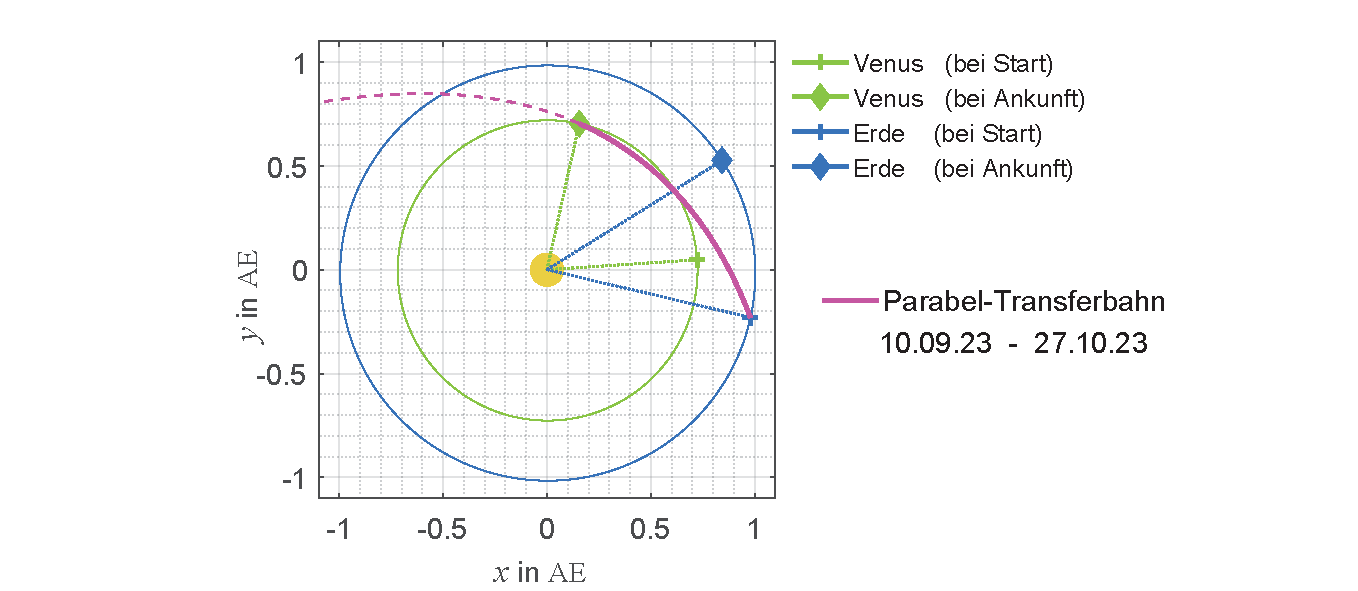
\includegraphics[width=\textwidth]{ParabelTransferVenus.pdf} 
	\caption[Parabel-L�sung des Lambert-Problems.]{Parabel-L�sung des Lambert-Problems f�r einen Flug zur Venus. Siehe \mscr~\mladynref{FlugVenusParabelbahn.m}.}
	\label{abb:adyn_lambert_lsg05}
\end{figure}

F�r die Berechnung der Transferbahn (elliptisch) von der Erde zur Venus oder zum Mars bei vorgegebener ToF benutzen wir die \mscr~\mladynref{LambertProblem03.m} \bzw \mladynref{LambertMarsVenus.m}, in welchen �ber die Routine \mladyniref{LambertSolver3.m}. die Parameter des interplanetaren Raumflugs zum Mars bzw. zur Venus �ber die L�sung des Lambert-Problems berechnet werden. Vorgegeben sind dabei die Positionsvektoren 1 und 2, sowie die Abflug und Ankunftszeit. Die Abflugs-Ankunfs-Positionen m�ssen vorher berechnet werden (z.B. �ber \mscr~\mladynref{FlugzeitenMarsVenus.m} oder �ber Programme aus dem Kapitel Himmelsmechanik, wie \mscr~\mlhmref{PlanetenbahnenKepler.m} und \mlhmref{PlanetenPositionen.m}. \\

\begin{figure}[H]
	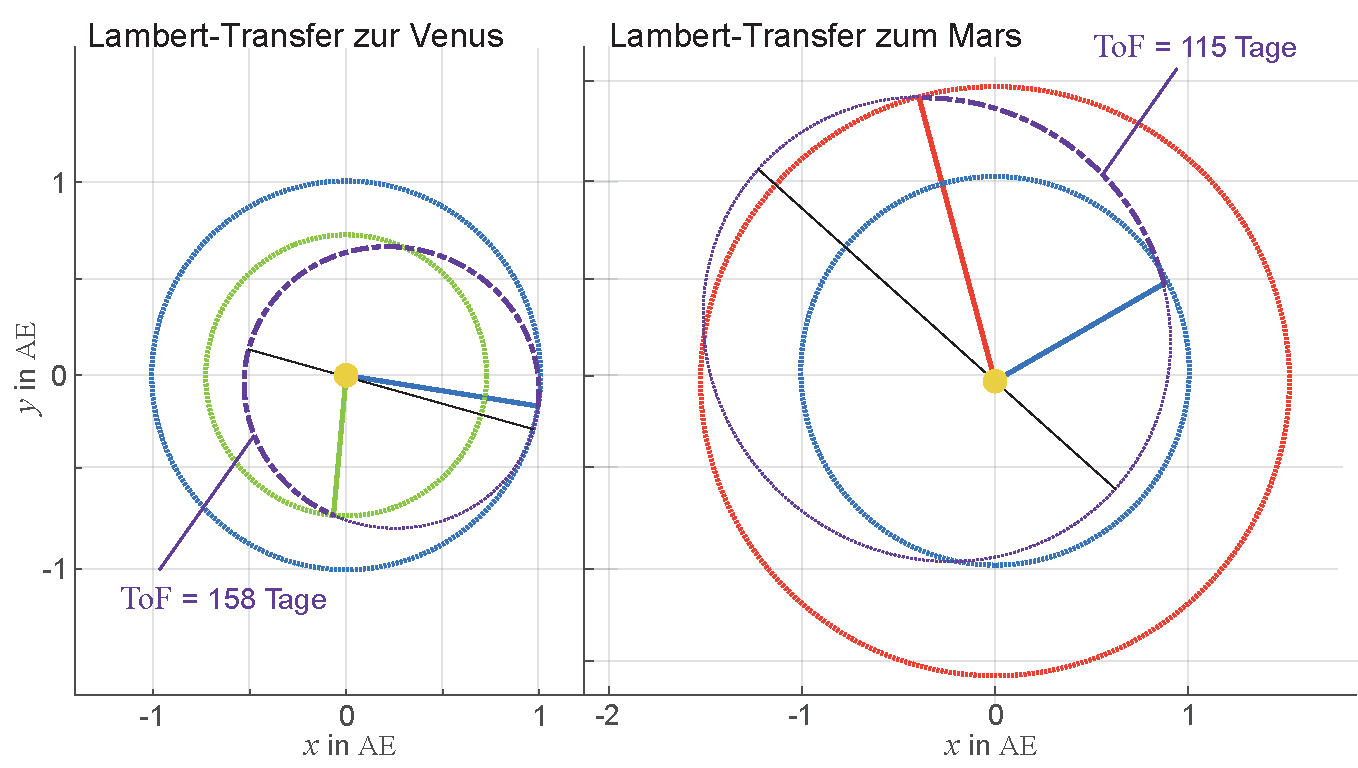
\includegraphics[width=\textwidth]{LambertTransferVenusMars.pdf} 
	\caption[L�sung des Lambert-Problems f�r Fl�ge zu Venus und Mars.]{L�sung des Lambert-Problems f�r Fl�ge zu Venus und Mars. Siehe \mscr~\mladynref{LambertProblem03.m}.}
	\label{abb:adyn_lambert_lsg06}
\end{figure}

\end{sol} 
\textcolor{blue} {$\rightarrow$ zur} \probref{adyn_manoevers5}.\\
\noindent\rule[1ex]{\textwidth}{0.5pt}  \newpage  \clearpage

%-----------------------------------------------------------------------------------------------------------

\begin{sol}{prob:adyn_manoevers6}\label{lsg:adyn_manoevers6} %�bung17
\textbf{Abfang ballistischer Raketen}\\

Die L�sung ist  im \mscr~\mladynref{LambertICBM.m} detailliert und mit ausf�hrlichen Kommentaren hinterlegt.
Die Vorgehensweise ist dabei wie folgt:
\begin{enumerate}[1.]
	\item Aus den gegebenen Werten f�r $\vec{R}$ und $\vec{V}$ der ICBM bestimmt man die Bahnparameter der ICBM. Wir verweisen auf \probref{adyn_orbits1}.
	\item Man berechnet mit diesen Bahnparametern �ber die Kepler-Gleichung \bzw die Methode mit den Gau�-Vektoren (PQR) (siehe \kap{hm_bahnen_hk_PQR}) den zeitlichen Verlauf der Trajektorie der ICBM und insbesondere den Punkt $\vec{R}(t_1+\mathrm{ToF})$, den diese nach $\mathrm{ToF}=\SI{30 }{\minute}$ errreicht. Wir erhalten:
\begin{align}
    \vec{R}(t_1+\mathrm{ToF})=[3930.7, 9762.2, 1583.3]\,\SI{}{\km}\,.
\end{align}
	\item F�r den Abf�nger gilt das Lambert-Problem mit $[\mathrm{P}_1,\mathrm{P}_2] = [\vec{r}(t_1), \vec{R}(t_1+\mathrm{ToF})]$.
	\item Man �berpr�ft, ob es �berhaupt eine L�sung geben kann. Dazu bestimmt man die minimale Flugzeit zu $t_\text{par} = \SI{16.0}{\minute}$ und die maximale Flugzeit zu $t_\text{m} = \SI{33.6}{\minute}$. Unsere $\mathrm{ToF}$ liegt dazwischen, es gibt also eine L�sung.
	\item Wir l�sen das Lambert-Problem wieder durch das in \probref{adyn_manoevers4} eingef�hrte Bisektionsverfahren und erhalten:
\begin{align}
    a=\SI{6130.7}{\km}\,,~~~\alpha = 2.9841\,,~~~\beta = 1.5418\,.
\end{align}
	\item Wir bestimmen mit diesen $a$, $\alpha$ und $\beta$ noch die notwendige Geschwindigkeit $\vec{v}_\text{trans}(t_1)$, die der Abf�nger am Punkt $\mathrm{P}_1$ haben muss, damit er auf die richtige Abfangbahn gelangt. Sie ergibt sich aus \eqref{eq:adyn_lambert08}zu:
\begin{align}
    \vec{v}_\text{trans}(t_1) &= (A+B)\,\vec{e}_c - (A-B)\,\vec{e}_1 = [2.16, 6.61, 1.13]\,\SI{}{\km\per\second}\, \\
		&\text{mit}\nonumber\\
		A &= \sqrt{\frac{G\,m_\text{E}}{4a}}\,\cot\frac{\alpha}{2}\,~~~~B = \sqrt{\frac{G\,m_\text{E}}{4a}}\,\cot\frac{\beta}{2}\,.\nonumber
\end{align}	
	\item Damit kann man sofort den erforderlichen Antriebsbedarf ermitteln, den man aufbringen muss, um den Abf�nger auf den richtigen Kurs zu bringen. Man erh�lt:
	\begin{align}
    \Delta \vec{v} &= \vec{v}_\text{trans}(t_1) - \vec{v}_1 = [4.66, 0.12,-1.37]\,\SI{}{\km\per\second}\,.		\\
		&\text{bzw}\nonumber\\
    \Delta v &= \SI{4.863}{\km\per\second}\,.
\end{align}	
	\item Zum Schlu� kann man aus $\vec{v}_\text{trans}(t_1)$ und $\vec{r}_1$ noch analog \probref{adyn_orbits1} die Bahnparameter der Abfangbahn berechnen und daraus mittels der Gau�-Vektoren-Methode (siehe \kap{hm_bahnen_hk_PQR}) die Trajektorie des Abf�ngers bestimmen, der sein Ziel nach genau 30 min erreicht (\figref{LambertAbfangICBM}).
\end{enumerate}

\begin{figure}[H]
	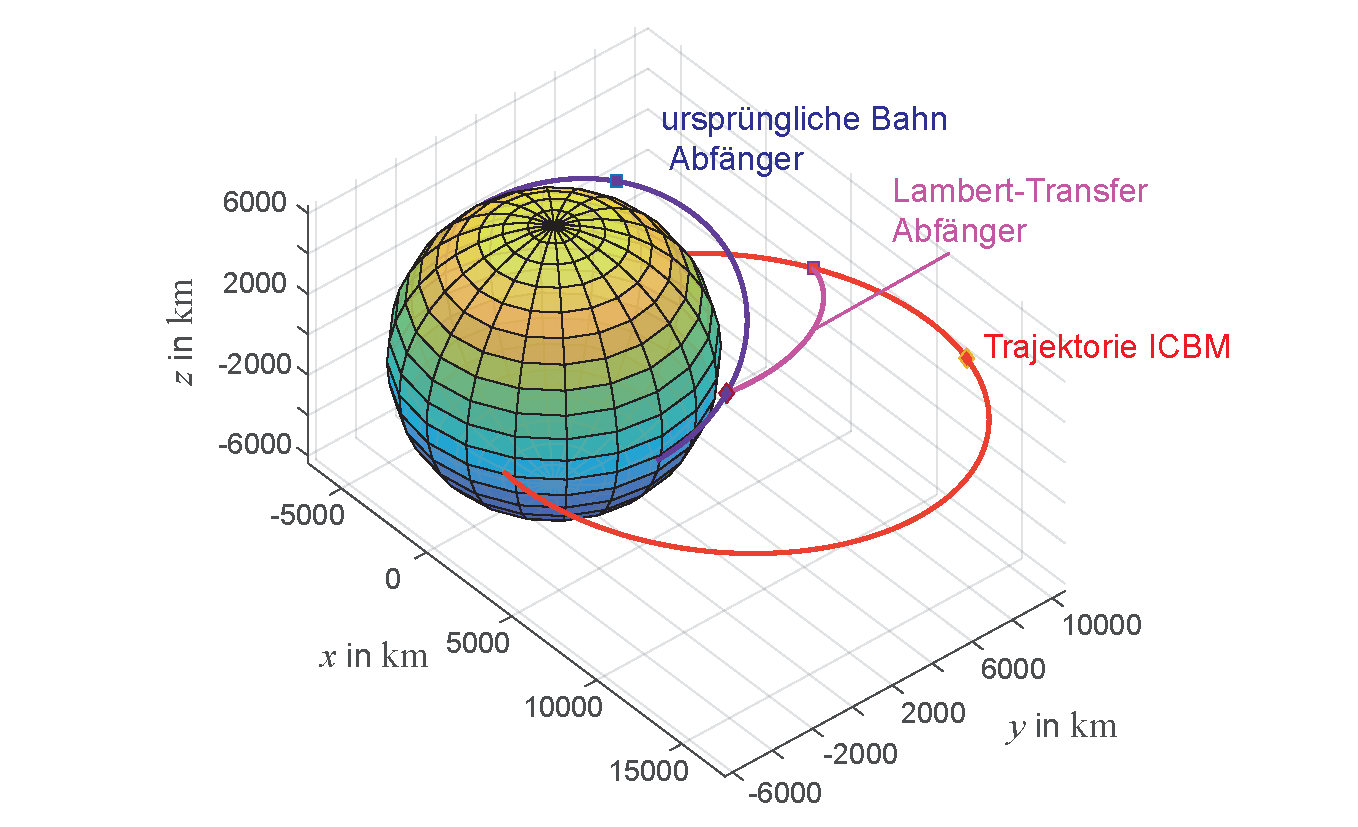
\includegraphics[width=\textwidth]{LambertAbfangICBM.pdf} 
	\caption[Abfang ballistischer Raketen.]{Abfang ballistischer Raketen. Dargestellt sind die Trajektorien der ICBM und des Abf�ngers mit und ohne $\Delta v$. Parameter siehe Text.}
	\label{abb:LambertAbfangICBM}
\end{figure}


\end{sol} 
\textcolor{blue} {$\rightarrow$ zur} \probref{adyn_manoevers6}.\\
\noindent\rule[1ex]{\textwidth}{0.5pt}  \newpage  \clearpage

%-----------------------------------------------------------------------------------------------------------

\begin{sol}{prob:adyn_manoevers7}\label{lsg:adyn_manoevers7} %�bung18
\textbf{Mondflug mit Ionenstrahltriebwerk}

\begin{itemize}
	\item
	Die Rechnungen sind im \mscr~\mladynref{Ionenantrieb02.m} ausgef�hrt und in \figref{IonenantriebExakt} dargestellt. Man sieht, dass die N�herung von \kap{adyn_kont_maneuver} zusammenbricht, wenn die Radius�nderung der Bahn per Umlauf gr��er wird.

\begin{figure}[H]
	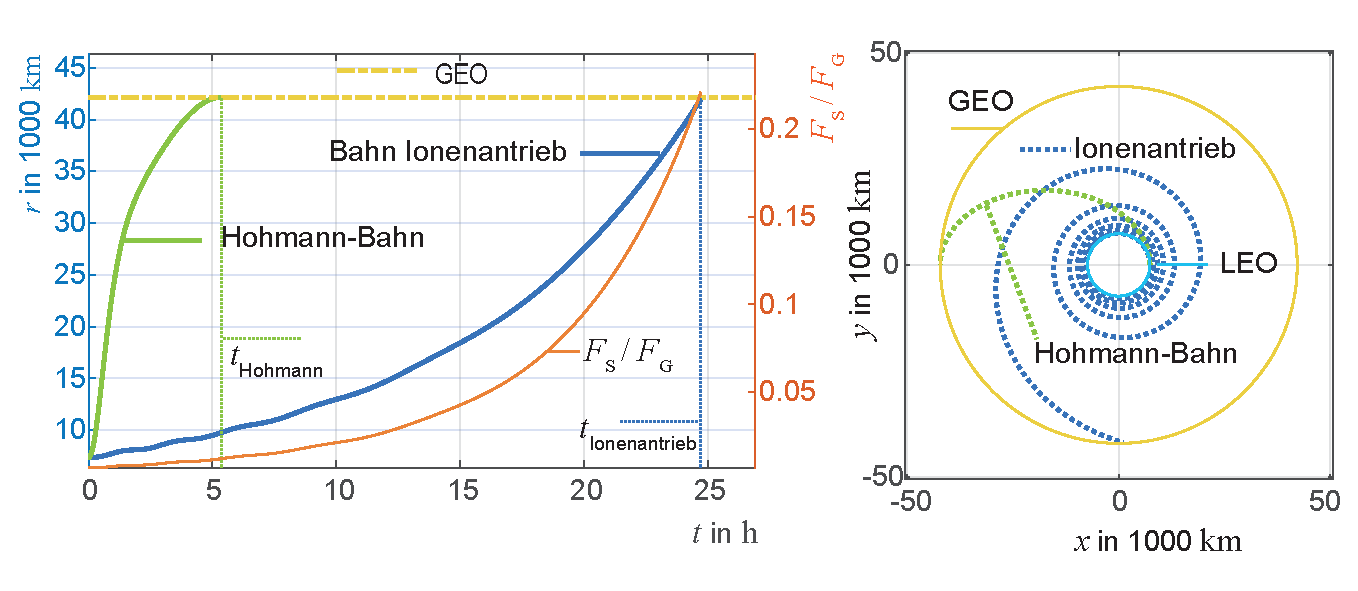
\includegraphics[width=\textwidth]{IonenantriebExakt.pdf} 
	\caption[Vergleich Hohmann-Transfer und Ionenantrieb.]{Vergleich Hohmann-Transfer und Ionenantrieb (LEO zu GEO), numerische L�sung der Bewegungsgleichung \eqref{eq:adyn_ionentr_01} f�r ein Triebwerk mit kontinuierlichem Schub. F�r den Ionenantrieb wurde ein konstanter Schub von $\SI{0.5}{\newton}$ angesetzt. Der Massenaussto� wurde bei der numerische Rechnung ber�cksichtigt.}
	\label{abb:IonenantriebExakt}
\end{figure}

	\item Die Rechnungen sind im \mscr~\mladynref{IonenantriebMond.m} ausgef�hrt. Dabei wurde die Triebwerksleistung entlang der Bahn linear so reduziert, dass sie bei der Entfernung, die dem Abstand des Lagrange-Punkts $\text{L}_1$ zwischen Erde und Mond entspricht, Null wird. Danach bewegt sich die Sonde allein im Gravitationsfeld des Mondes. Der Hohmann-Transfer wurde ebenfalls unter Ber�cksichtigung der Gravitationswirkung des Mondes berechnet.
Das Ergebnis der Rechnungen ist in der \figref{IonenantriebMoon} zu sehen.

\begin{figure}[H]
	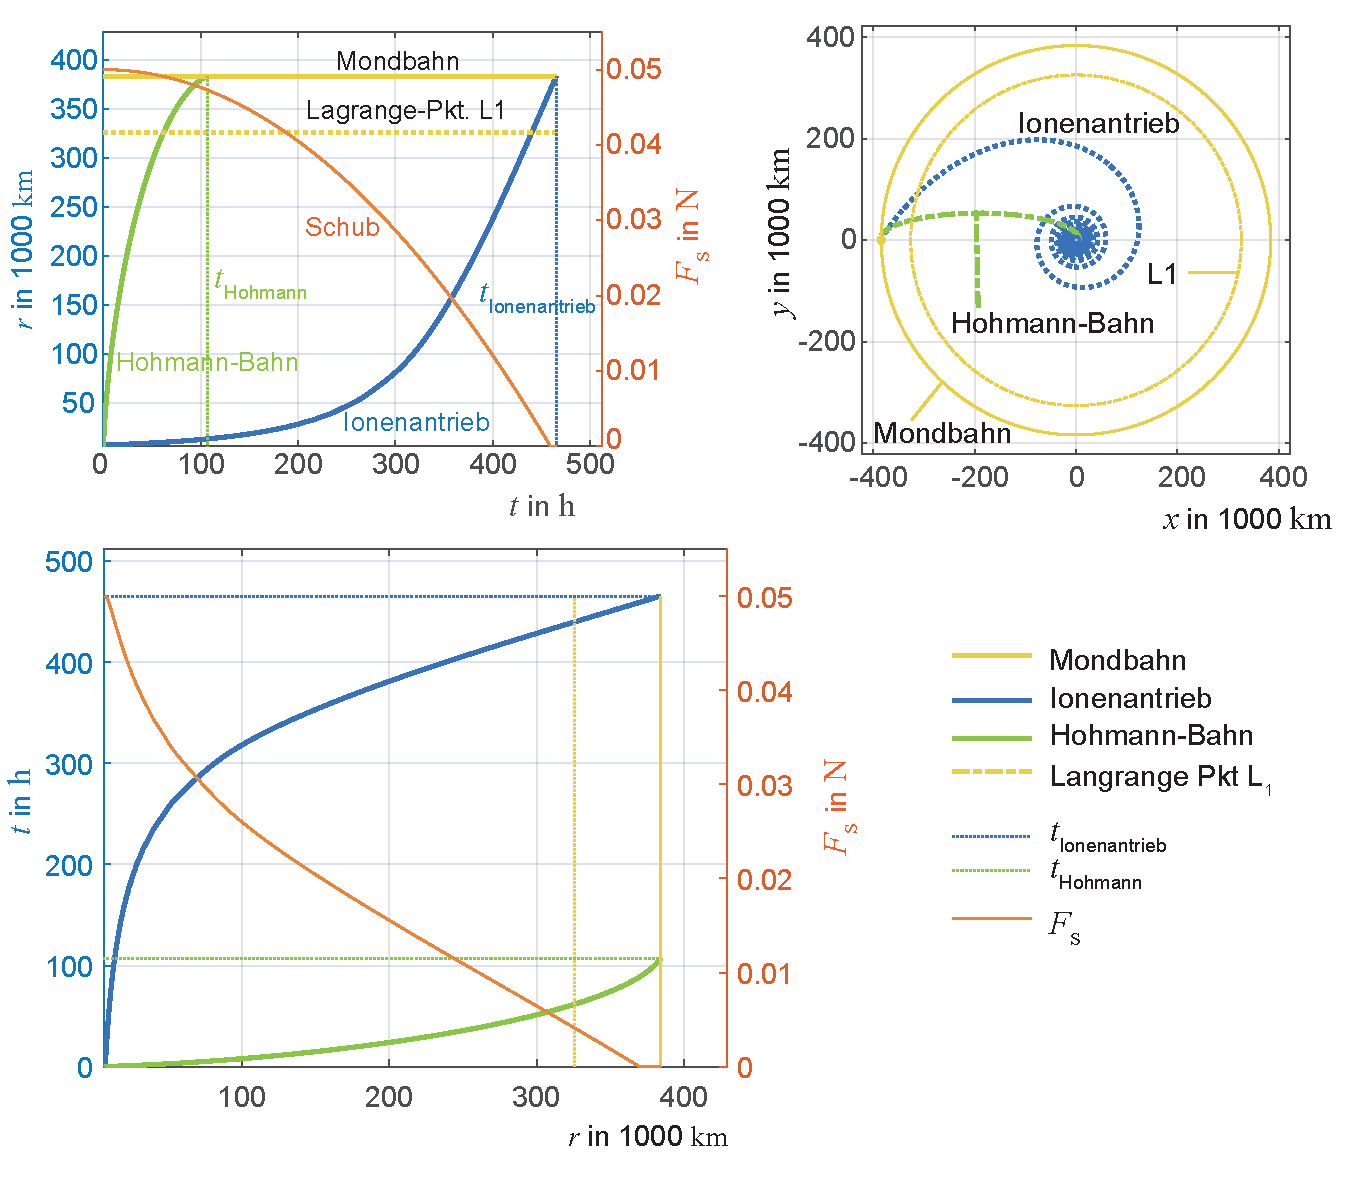
\includegraphics[width=\textwidth]{IonenantriebMoon.pdf} 
	\caption[Vergleich Hohmann-Transfer und Ionenantrieb zum Mond.]{Vergleich Hohmann-Transfer und Ionenantrieb zum Mond. F�r den Ionenantrieb wurde ein initialer Schub von $\SI{0.05}{\newton}$ der bis zum Gravitationsgleichgewicht zwischen Erde und Mond kontinuierlich reduziert wurde. Ebenso wurde der Massenaussto� bei der numerische Rechnung ber�cksichtigt.}
	\label{abb:IonenantriebMoon}
\end{figure}

\end{itemize}

\end{sol} 
\textcolor{blue} {$\rightarrow$ zur} \probref{adyn_manoevers7}.\\
\noindent\rule[1ex]{\textwidth}{0.5pt}  \newpage  \clearpage

%-----------------------------------------------------------------------------------------------------------

\begin{sol}{prob:adyn_SOI}\label{lsg:adyn_SOI} %�bung19
\textbf{Einflusssph�re - Sphere of Influence (SOI)}\\

Die Begriffe Hill-Sph�re\index{Hill-Sph�re} und Einflusssph�re\index{Einflusssph�re}\index{Sphere of Influence, SOI} adressieren zwei unterschiedliche Probleme:\\

\textit{Hill Sph�re:} Gegeben sind eine gro�e Masse $m_1$ (\zb die Sonne) und eine etwas kleinere Masse $m_2 < m_1$ (\zb die Erde) gegeben. Letztere bewegt sich um die gr��ere Masse. Es wird der Bereich gesucht, in dem f�r eine noch kleinere Masse $m_\text{M}$ (\zb der Mond) eine stabile Bahn um die kleine Masse ($m_2$) m�glich ist. Dieser Bereich wird Hill-Sph�re genannt. Die Berechnung der Hill-Sph�re hatten wir in \probref{hm_hill_sphere} ausf�hrlich behandelt und hatten dor mit $a$ als den Abstand zwischen den Massen $m_1$ und $m_2$ erhalten \eqref{eq:hm_moon_moon_lsg9}:
\begin{equation}
	r_\text{H} = a\,\sqrt[3]{\frac{1}{3}\frac{m_1}{m_2}} \,. \label{eq:adyn_hill_sphere_radius}:
\end{equation}

\textit{SOI:} Hier sind nun zwei relativ gro�e Massen $m_1, m_2$ gegeben (\zb Mars $m_1$ und Jupiter $m_2$ oder Sonne $m_2$ und Mars $m_1$ ) und eine sehr kleine Masse $m_\text{R}$ (\zb eine Raumsonde), die sich zwischen diesen beiden Massen bewegt. Es werden die Bereiche gesucht, in welchem jeweils eines der Zentren der Massen $m_1, m_2$ den Ursprung des Koordinatensystems bildet, welches f�r die Beschreibung der Bewegung der sehr kleinen Masse $m_\text{R}$  verwendet wird. In diesem Bereich muss dann f�r die Berechnung der Bewegung nur die Gravitationskraft der jeweiligen die SOI definierenden Masse $m_1$ oder $m_2$ ber�cksichtigt werden. Damit kann in der Astrodynamik bei interplanetaren Raumfl�gen die Trajektorie oft durch Aneinanderf�gen von Kepler-Bahn Abschnitten in den aufeinanderfolgenden SOI der einzelnen Planeten \bzw der Sonne (im interplanetaren Raum) n�herungsweise berechnet werden (sogenannte \textit{patched conic trajectories}.\\
Zur Herleitung der Beziehung f�r den Radius der SOI als Funktion der Massen  $m_1, m_2$ verwendet man zwei Referenzsysteme:
\begin{itemize}
	\item Zum einen erfolgt die Betrachtung der Bewegung der Raumsonde in einem Koordinaten\-system, dessen Ursprung im Zentrum der Masse $m_1$ liegt und ber�cksichtigt als Hauptwirkung nur die Gravitation der Masse $m_1$. Die Gravitationsbeschleunigung der gr��eren Masse $m_2$ wird in der Bewegungsgleichung als St�rgr��e eingef�hrt, im Prinzip als erste Abeitung.
	\item Dann betrachtet man die Bewegung der Raumsonde in dem \KOS, dessen Ursprung im Zentrum der Masse $m_2$ liegt und ber�cksichtigt als Hauptwirkung nur die Gravitation der Masse $m_2$. In der Bewegungsgleichung wird dann wiederum die Gravitationsbeschleunigung der Masse $m_1$ als St�rgr��e eingef�hrt.
\end{itemize}

\begin{figure}[H]
	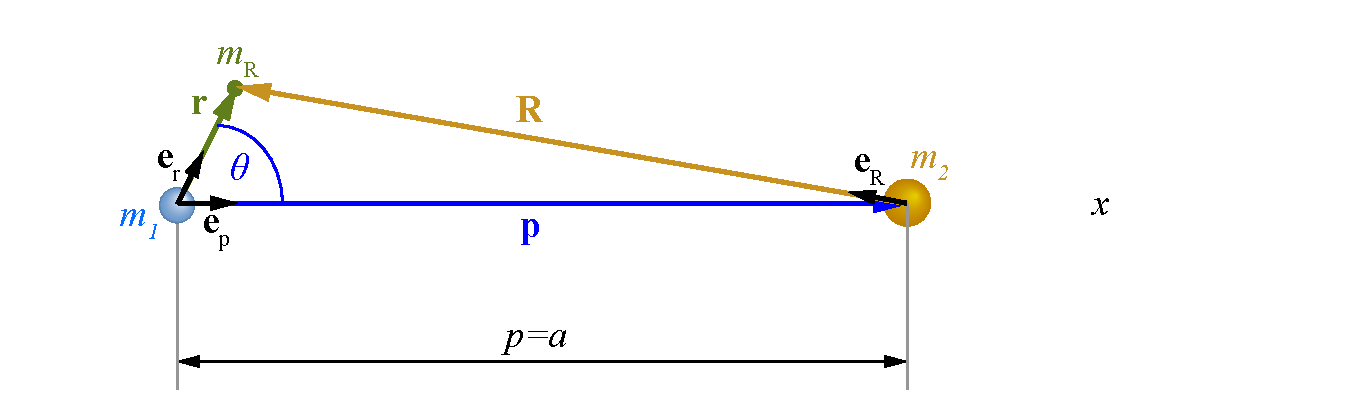
\includegraphics[width=\textwidth]{GeometrieHerleitungSOI.pdf} 
	\caption[Zur Herleitung der Einflusssph�re.]{Zur Herleitung der Einflusssph�re.}
	\label{abb:adyn_SOI01}
\end{figure}

Es ergeben sich folgende Bewegungsgleichungen (f�r $m_\text{R} \ll m_1,m_2$):\footnote{Die Herleitung wird als Zusatz�bung empfohlen, siehe auch \kap{hm_potentialtheorie} sowie \figref{adyn_SOI01}.}
\begin{subequations}
\begin{align}
    \ddot{\vec{r}} &= -G\,m_1\,\frac{\vec{r}}{r^3}-G\,m_2\,\lk\frac{\vec{p}}{p^3} + \frac{\vec{R}}{R^3}\rk\,,\\
    \ddot{\vec{R}} &= -G\,m_2\,\frac{\vec{R}}{R^3}-G\,m_1\,\lk\frac{\vec{r}}{r^3} - \frac{\vec{p}}{p^3}\rk\,.
\end{align}    \label{eq:adyn_SOI01}
\end{subequations}

Diese Gleichungen k�nnen geschrieben werden als:
\begin{subequations}
\begin{align}
     \ddot{\vec{r}} &= \vec{a}_{\text{H},1}^{\lk 1 \rk} + \vec{a}_{\text{S},2}^{\lk 1 \rk}\,, \\
     \ddot{\vec{R}} &= \vec{a}_{\text{H},2}^{\lk 2 \rk} + \vec{a}_{\text{S},1}^{\lk 2 \rk} \,,
\end{align} \label{eq:adyn_SOI02}
\end{subequations}

worin in $\vec{a}_{\text{H,S},i}^{\lk j \rk}$ der Index $j$ das KOS-System des jeweiligen Planeten bezeichnet und H und S f�r die Hauptgravitations- \bzw St�rbeschleunigung stehen. Letztere wird hervorgerufen jeweils durch die Masse $m_i$ ($i=1,2$). Die Beschleunigungen k�nnen mit den Einheitsvektoren $\vec{e}_\text{r},\, \vec{e}_\text{R}$ und $\vec{e}_\text{p}$aus \figref{adyn_SOI01} beschrieben werden durch:

\begin{subequations}
\begin{align}
   \vec{a}_{\text{H},1}^{\lk 1 \rk} &= -\frac{G\,m_1}{r^2}\,\vec{e}_\text{r}\,,\label{eq:adyn_SOI03a} \\ 
    \vec{a}_{\text{H},2}^{\lk 2 \rk} &= -\frac{G\,m_2}{R^2}\,\vec{e}_\text{R}\,, \label{eq:adyn_SOI03b} \\
    \vec{a}_{\text{S},2}^{\lk 1 \rk} &= +\,G\,\frac{m_2}{p^2}\,\sum\limits_{k=1}^\infty \lk \frac{r}{p}\rk^k\lek {\PL {k+1}}'\lk  \cos\theta\rk\,\vec{e}_\text{p} - {\PL {k}}'\lk\cos\theta\rk\,\vec{e}_\text{r} \rek\,, \label{eq:adyn_SOI03c} \\ 
    \vec{a}_{\text{S},1}^{\lk 2 \rk}&= +\,G\,\frac{m_1}{r^2}\,\lek \lk \frac{r}{p} \rk^2\,\vec{e}_\text{p} - \vec{e}_\text{r} \rek\,, \label{eq:adyn_SOI03d}
\end{align} \label{eq:adyn_SOI03}
\end{subequations}  

worin $\PL k$ die im \kap{hm_potentialtheorie} eingef�hrten Legendre-Polynome sind (\cite{Andrews2003}) und ${\PL k}'$ deren erste Ableitungen. 
Die Gleichungen sind direkt aus \eqref{eq:adyn_SOI01} ablesbar. Lediglich Gleichung \eqref{eq:adyn_SOI03b} erfordert eine Nebenrechnung. Sie ergibt sich aus der Definition der Legendre-Polynome und der Nutzung der verschiedenen Beziehungen zwischen den Ableitungen und den Rekursionsformeln (\cite{Riley2006, Andrews2003}). 
Wir bilden nun die Verh�ltnisse von Hauptbeschleunigung zu St�rbeschleunigung im jeweiligen \KOS. Wir dividieren dazu \eqref{eq:adyn_SOI03d} durch \eqref{eq:adyn_SOI03b} und finden:
\begin{align}
    \frac{ \vec{a}_\text{S1}^{\lk 2\rk}}{ \vec{a}_\text{H2}^{\lk 2\rk}} = \frac{m_1}{m_2}= \frac{1-2\,\lk\frac{r}{p}\rk\,\cos\theta + \lk\frac{r}{p}\rk^2}{\lk\frac{r}{p}\rk^2}\,\sqrt{\lek 1-2\,\lk\frac{r}{p}\rk^2\,\cos\theta + \lk\frac{r}{p}\rk^4\rek} \,.\label{eq:adyn_SOI04}
\end{align}
Analog erh�lt man durch Division von \eqref{eq:adyn_SOI03c} durch \eqref{eq:adyn_SOI03a}:
\begin{align}
    \frac{\vec{a}_{\text{S},2}^{\lk 2\rk}}{\vec{a}_{\text{H},1}^{\lk 2\rk}} = \frac{m_1}{m_2}\,\lk \frac{r}{p} \rk^3 \, \sqrt{\lek 1+3\cos^2\theta \rek} + \mathcal{O}\lk\frac{r}{p}^4\rk \,, \label{eq:adyn_SOI05}
\end{align}
wobei wir hier wegen $r \ll p$ alle Terme mit Potenzen von $\lk \frac{r}{p} \rk^n$, $n>3$ vernachl�ssigen. Die Gleichungen dr�cken das Verh�ltnis von St�rbeschleunigung zu Hauptbeschleunigung im jeweiligen Bezugssystem aus.\\
Gleichsetzen von \eqref{eq:adyn_SOI04} mit \eqref{eq:adyn_SOI05} bedeutet, dass die St�rungs- und Hauptbeschleunigungen an einem Ort im Abstand $r_\text{SOI} $ von dem jeweiligen Zentrum des \KOS im gleichen Verh�ltnis zueinander stehen. Man erh�lt dann eine diesen Abstand unter der Annahme $r/p \ll 1$: 
\begin{align}
    \frac{r_\text{SOI}}{p} &= \sqrt[5]{\frac{m_1{}^2}{m_2{}^2}}\,\underbrace{\lk 1+3\cos^2\theta\rk^{-\frac{1}{10}}}_{\leq 1.148}~~\rightarrow ~~~ \frac{r_\text{SOI}}{p} \approx \lk \frac{m_1}{m_2}\rk^{\frac{2}{5}}\,. \label{eq:adyn_SOI06}
\end{align}
Der Radius einer SOI h�ngt somit vom Abstand $p$ beider Massen und dem Verh�ltnis (hoch $2/5$) der beiden Massen ab. Tabelle \ref{tab:adyn_SOI01} zeigt die Radien der SOI der Planeten unseres Sonnensystems im Vergleich zu den Radien der Hill-Sph�re \eqref{eq:adyn_hill_sphere_radius}:
\begin{table}[ht]
		\begin{center}
    \begin{tabular}{|C{1.5cm}|C{2.75cm}|C{2.75cm}|C{2.75cm}|C{2.75cm}|}
    \hline
    \rule{0pt}{3pt}& & &&  \\
      Planet (Masse $m_1$) & Gro�e Halbachse\linebreak zur Sonne \linebreak (Masse $m_2$)\linebreak $\lk\SI{}{\km}\rk$ & Massenverh�ltnis Planet/Sonne \linebreak $m_1/m_2$& Radius der SOI \linebreak  $\lk\SI{}{\km}\rk$ \linebreak \linebreak \eqref{eq:adyn_SOI_radius} &  Radius der Hill-Sph�re  \linebreak  $\lk\SI{}{\km}\rk$ \linebreak \linebreak \eqref{eq:adyn_hill_sphere_radius} \\
    \rule{0pt}{3pt}&& &&  \\
    \hline
    \rule{0pt}{3pt}&& &&   \\
    \rule{0pt}{6pt} Merkur &\SI{57.9e6}{}&$\SI{0.166e-6}{}$ & $\SI{112000e06}{}$& $\SI{2.206e05}{}$\\
    \rule{0pt}{3pt}&& &&   \\
    \rule{0pt}{6pt} Venus &\SI{108.2e6}{}&$\SI{2.450e-6}{}$ & $\SI{616350e06}{}$& $\SI{1.010e+06}{}$\\
    \rule{0pt}{3pt}&& &&   \\
    \rule{0pt}{6pt} Erde & \SI{149.6e6}{}&$\SI{3.002e-6}{}$ & $\SI{924510e06}{}$& $\SI{1.496e+06}{}$\\
    \rule{0pt}{3pt}&& &&   \\
    \rule{0pt}{6pt} Mars &\SI{227.9e6}{}&$\SI{0.323e-6}{}$ & $\SI{577230e06}{}$& $\SI{1.084e+06}{}$\\
    \rule{0pt}{3pt}&& &&   \\
    \rule{0pt}{6pt} Jupiter &\SI{778.6e6}{}&$\SI{954.490e-6}{}$ & $\SI{48219000e06}{}$& $\SI{5.315e+07}{}$\\
    \rule{0pt}{3pt}&& &&   \\
    \rule{0pt}{6pt} Saturn &\SI{1433.5e6}{}&$\SI{285.641e-6}{}$ & $\SI{54793000e06}{}$& $\SI{6.546e+07}{}$\\
    \rule{0pt}{3pt}&& &&   \\
    \rule{0pt}{6pt} Uranus &\SI{2872.5e6}{}&$\SI{43.651e-6}{}$ & $\SI{51791000e06}{}$& $\SI{7.013e+07}{}$\\
    \rule{0pt}{3pt}&& &&   \\
    \rule{0pt}{6pt} Neptun &\SI{4495.1e6}{}&$\SI{51.295e-6}{}$ & $\SI{86451000e06}{}$& $\SI{1.158e+08}{}$\\
    \rule{0pt}{3pt}&& &&   \\
    \hline
    \end{tabular} 
		\end{center}
		\caption{Vergleich Radien der SOI mit dem Hill-Sph�re f�r die Planeten unseres Sonnensystems.}
		\label{tab:adyn_SOI01}
\end{table}

Im letzten Schritt in \eqref{eq:adyn_SOI06} haben wir die $\theta$-Abh�ngigkeit vernachl�ssigt. Ber�cksichtigt man diese, so ergibt sich ein oblater Sph�roid anstelle einer Einflusssph�re (Sphere of Influence). In den meisten F�llen reicht die Kugelbetrachtung aber aus, man kann also schreiben:
\begin{align}
	r_\text{SOI} = a\,\sqrt[5]{\lk \frac{m_1}{m_2}\rk^2} \,, \label{eq:adyn_SOI_radius}
\end{align}
worin a der Abstand zwischen den beiden Massen (\ia gleich der gro�en Halbachse von $m_1$ um $m_2$) ist.\\
Man wird also immer dann, wenn sich die Raumsonde in geringerem Abstand als $r_\text{SOI}$  von der Masse $m_1$ befindet, die Bewegung als Zweik�rperproblem mit den Massen $m_1,\,m_\text{R}$ behandeln k�nnen, bei Abst�nden gr��er als $r_\text{SOI}$ als Zweik�rperproblem mit den Massen $m_2,\,m_\text{R}$.\\

\end{sol} 
\textcolor{blue} {$\rightarrow$ zur} \probref{adyn_SOI}.\\
\noindent\rule[1ex]{\textwidth}{0.5pt}  \newpage  \clearpage

%-----------------------------------------------------------------------------------------------------------

\begin{sol}{prob:adyn_swingby01}\label{lsg:adyn_swingby01} %�bung20
\textbf{Gravity-Assist-Man�ver - Analytische L�sung}\\

Wir beginnen mit:
\begin{subequations}
\begin{align}
        \vec{v}_1{}' &= \vec{v}_1 - \vec{v}_\text{P} \,, \label{eq:adyn_lsgswingby01a} \\
        v_1{}'^2     &= v_1{}^2 + v_\text{P}{}^2 - 2\,v_1{}'\,v_\text{P}\,\cos\gamma_1{}'\,, \label{eq:adyn_lsgswingby01b} \\
        \vec{v}_2{}  &= \vec{v}_2{}' + \vec{v}_\text{P} \,, \label{eq:adyn_lsgswingby02a} \\
        v_2{}^2      &= v_2{}'^2 + v_\text{P}{}^2 + 2\,v_2{}'\,v_\text{P}\,\cos\beta_2{}' \,, \label{eq:adyn_lsgswingby02b} \\
        v_1{}'       &= v_2{}'= v_\infty \,. \label{eq:adyn_lsgswingby02c} 
\end{align} %\label{eq:adyn_lsgswingby02} 
\end{subequations}
F�r die weitere numerische Auswertung lassen sich aus \eqref{eq:adyn_swingby01}, \eqref{eq:adyn_swingby03} und \figref{adyn_swingby01} durch Anwendung des Kosinussatzes \bzw geometrische �berlegungen aus der Streuhyperbel noch einige n�tzliche Beziehungen, \zb zwischen dem Winkel $\beta_2{}'$ und dem Streuwinkel $\vartheta'$ sowie f�r den Winkel $\varphi'$ gewinnen:
\begin{subequations}
\begin{align}
        \beta_2{}' &= \beta_1{}' -\vartheta' = \beta_1{}' + 2\varphi' - 180\degree \label{eq:adyn_lsgswingby03a} \\
        \cos\beta_2{}' &= \cos\,\beta_1{}'\,\lk 1-2\cos^2\varphi'\rk + 2\cos\varphi'\,\sqrt{1-\cos^2\varphi'}\,\sqrt{1-\beta_1'{}^2} \label{eq:adyn_lsgswingby03b} \\
        \cos\beta_1{}' &= \frac{{v_1{}}^2+v_\text{P}{}^2-{v_1{}'}^2}{2\,v_1\,v_\text{P}} \label{eq:adyn_lsgswingby03c}
\end{align}%\label{eq:adyn_lsgswingby03} 
\end{subequations}
Die Gr��e $\cos\varphi'$ k�nnen wir ebenfalls aus \figref{adyn_swingby01} mit der Hyperbelgleichung durch
\begin{align}
    \cos\varphi' &= \frac{1}{1+ (r_\text{per}\,v_1{}'^2)/(G\,m_\text{P})} = -\frac{1}{e}\,\label{eq:adyn_lsgswingby04} 
\end{align}
ausdr�cken.

\begin{nebenrechnungNeu} {} \\
Der Winkel $\varphi'$ h�ngt mit dem asymptotischen Grenzwinkel $\theta_\infty{}'$ der Hyperbel wie folgt zusammen:
\begin{align}
    \theta_\infty{}' = -\frac{1}{e} = + \cos\lk 180\degree-\varphi'\rk = - \cos\varphi' \label{eq:adyn_lsgswingby05} 
\end{align}
Die Exzentrizit�t ist nach \eqref{eq:hm_relations2} gegeben durch
\begin{align}
    e= \sqrt{1+\frac{2\,H\,L^2}{\mu_\text{P}{}^2}} = \sqrt{1+\frac{2L^2}{\mu_\text{P}{}^2}\,\frac{v_1{}'^2}{2}} = \sqrt{1 + \frac{b^2\,v_1{}'^4}{\mu_\text{P}^2}}\,, \label{eq:adyn_lsgswingby06} 
\end{align}
wobei wir $H = v_1{}'^2/2$ f�r $r\to \infty$ und $L_\infty = b\,v_1{}' = b\,v_2{}' = b\, v_\infty$ f�r $r\to \infty$ benutzt haben.\\
Wegen der Drehimpulserhaltung k�nnen wir $L_\infty$ durch $L_\text{per} = r_\text{per}\,v_\text{per}{}'$ am Perizentrum ersetzen und benutzen dabei den \textit{vis-viva}-Satz \eqref{eq:hm_vis-viva}, womit wir erhalten:
\begin{align}
    L = b\,v_1{}' = r_\text{per}\,v_\text{per}{}'~~~\text{und}~~~
    \frac{v_1{}'}{2}^2 = \frac{v_\text{per}{}'^2}{2} - \frac{\mu_\text{P}}{r_\text{per}}\,.\label{eq:adyn_lsgswingby07} 
\end{align}
\end{nebenrechnungNeu}

\newpage
Mit den Beziehungen in \eqref{eq:adyn_lsgswingby07} k�nnen wir in \eqref{eq:adyn_lsgswingby06} den Streuparameter $b$ eliminieren und erhalten aus \eqref{eq:adyn_lsgswingby02b} mit \eqref{eq:adyn_lsgswingby05} �ber \eqref{eq:adyn_lsgswingby03b} schlie�lich die heliozentrische Geschwindigkeit des Raumschiffs $v_2$ beim Verlassen der Einflusssph�re des Gravity-Assist-Planeten am Punkt $\text{P}_2$:
\begin{subequations}
    \begin{align}
        v_2{}^2 = v_1{}^2 - \frac{2\,C_1}{C_2{}^2} + \frac{4\,v_1{}'\,v_\text{P}}{C_2}\,\sqrt{1-\frac{1}{C_2{}^2}}\,\sqrt{1-\lk\frac{C_1}{2\,v_1{}'\,v_\text{P}}\rk^2}\label{eq:adyn_lsgswingby08a}
    \end{align}
    mit 
    \begin{align}
        C_1 &= v_1{}^2 - v_\text{P}^2 - v_1{}'^2 \label{eq:adyn_lsgswingby08b}\,,\\
        C_2 &= 1+\frac{r_\text{per}}{\mu_\text{P}}\,v_1{}'{}^2 \label{eq:adyn_lsgswingby08c}\,,\\
        v_1{}'&= \sqrt{v_1{}^2 +v_\text{P}{}^2 - 2\,v_1\,v_\text{P}\,\cos\gamma_1}\,.\label{eq:adyn_lsgswingby08d}
    \end{align}%\label{eq:adyn_lsgswingby08}
\end{subequations}
Wir haben $v_2(r_\text{per},\gamma_1)$ in \figref{adyn_lsgswingby01} dargestellt.

\begin{figure}[H]
	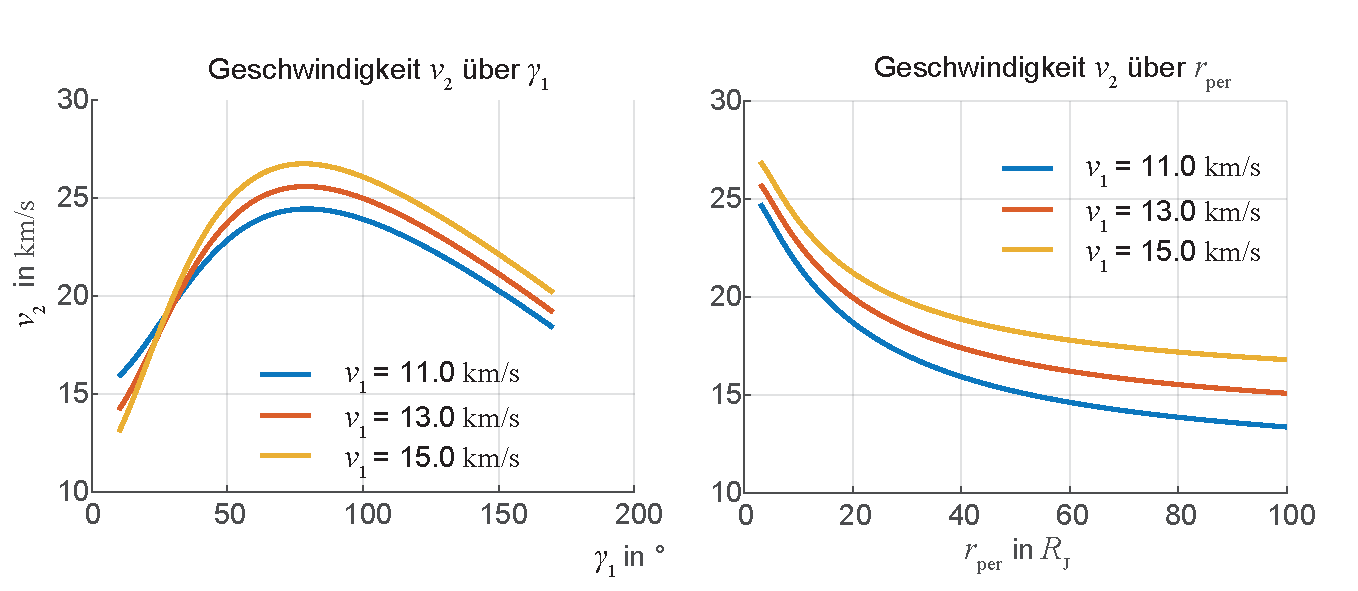
\includegraphics[width=\textwidth]{GravityAssistAnalytisch.pdf} 
	\caption[Gravity-Assist-Man�ver (Analytisch L�sung).]{Gravity-Assist-Man�ver (Analytisch L�sung).}
	\label{abb:adyn_lsgswingby01}
\end{figure}

Zum Schluss wollen wir noch den maximal m�glichen Energiegewinn bei einem Gravity-Assist-Man�ver berechnen. Dieser ergibt sich zu
\begin{align}
    \Delta H &= \frac{1}{2}\,v_2{}^2 - \frac{m_\text{S}\,G}{r_1-r_\text{per}} - \lk \frac{1}{2}\,v_1{}^2 - \frac{m_\text{S}\,G}{r_1-r_\text{per}}\rk \approx \frac{1}{2}\,\lk v_2{}^2 - v_1{}^2\rk \,.\label{eq:adyn_lsgswingby09}
\end{align}
Der Energiegewinn h�ngt also bei vorgegebenen $r_\text{per}$ von zwei Parametern ab:\\
$v_1{}'$ (\bzw. $v_1$)\, und $\beta_1{}'$ (\bzw $\gamma_1$).
Tr�gt man $\Delta H$ �ber $\beta_1{}'$ und $v_1{}'$ auf, so findet man ein Maximum bei $\beta_1{}' = 2\pi/3=120\degree$ und 
	\[v_1{}' = \sqrt{\frac{\mu_\text{P}}{r_\text{per}}}\,,
\]
Damit kann man mit den bekannten Gr��en $m_\text{P}$, $r_\text{per}$ (wir nehmen $r_\text{per} \approx 5\,R_\text{P}$ an) und $v_\text{P}$ die notwendig Anfluggeschwindigkeit $v_\text{1,opt}$ bestimmt, die den maximalen Energiegewinn bringt. Die Rechnungen sind im Detail \mscr{} \mladynref{GravityAssistAnalytik.m} ausgef�hrt. 

Der Energiegewinn $\Delta H(v_1{}', \beta_1{}')$ \bzw $\Delta H(v_1{}, \gamma_1{})$ ist in \figref{adyn_lsgswingby02a} dargestellt:

\begin{figure}[H]
	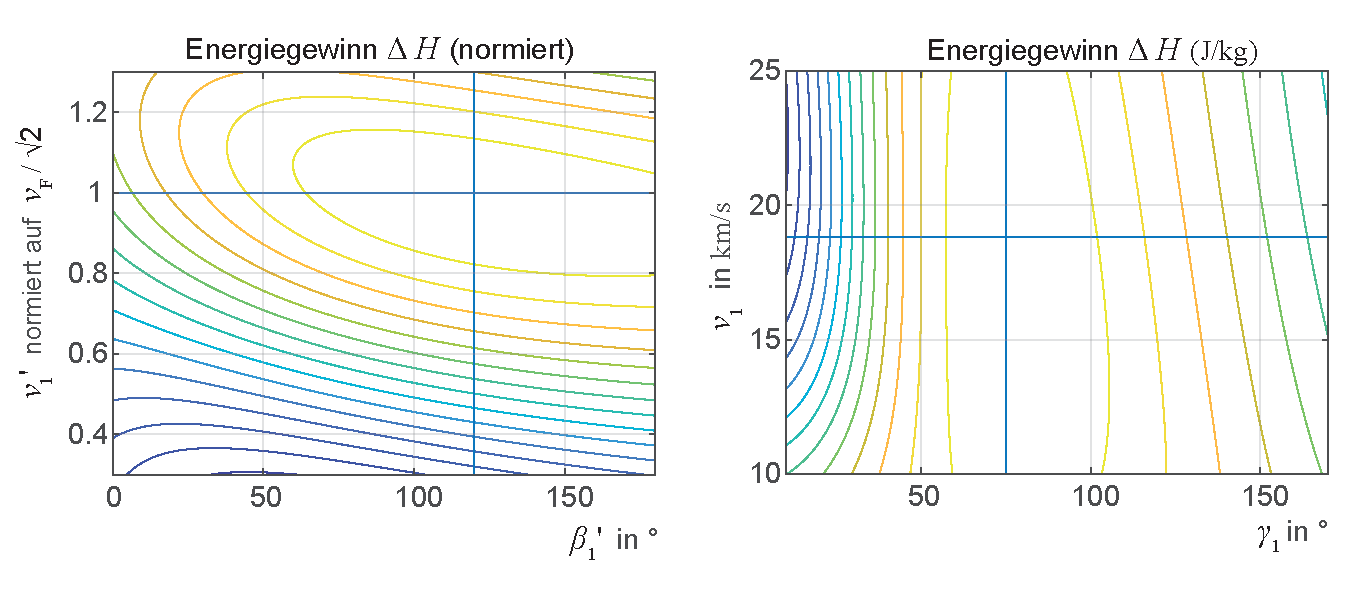
\includegraphics[width=\textwidth]{GravityAssistEnergiegewinn.pdf} 
	\caption[Gravity-Assist-Man�ver - Energiegewinn.]{Gravity-Assist-Man�ver - Energiegewinn am Beispiel des Flugs einer Raumsonde um den Jupiter.  Parameter: $r>_\text{per} = 5\,R_\text{J}$.}
	\label{abb:adyn_lsgswingby02a}
\end{figure}

\end{sol} 
\textcolor{blue} {$\rightarrow$ zur} \probref{adyn_swingby01}.\\
\noindent\rule[1ex]{\textwidth}{0.5pt}  \newpage  \clearpage
%
%%-----------------------------------------------------------------------------------------------------------

\begin{sol}{prob:adyn_swingby03}\label{lsg:adyn_swingby03} %�bung21
\textbf{Gravity-Assist-Man�ver - Simulation}\\

Die Simulation des Swing-By ist im \mscr{} \mladynref{GravityAssistSimulation.m} ausgef�hrt, die Resultate f�r ein Beispiel am Jupiter in \figref{adyn_lsgswingby02}.\\

\begin{figure}[H]
	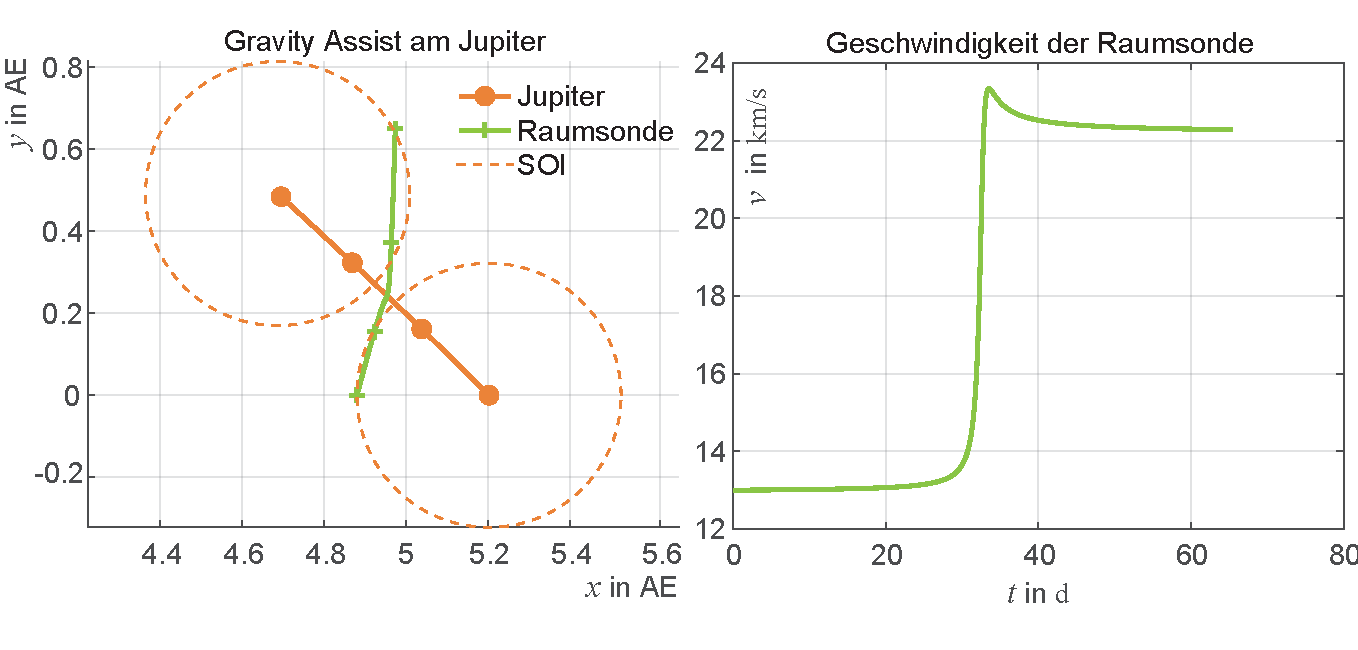
\includegraphics[width=\textwidth]{GravityAssistSimulation.pdf} 
	\caption[Gravity-Assist-Man�ver Simulation.]{Ergebnisse der Gravity-Assist-Man�ver Simulation im heliozentrischen \KOS am Beispiel des Flugs einer Raumsonde um den Jupiter.  Parameter: $v_1 = \SI{13.0}{\km\per\second}$, $\gamma_1 = 75\degree$.}
	\label{abb:adyn_lsgswingby02}
\end{figure}

\end{sol} 
\textcolor{blue} {$\rightarrow$ zur} \probref{adyn_swingby03}.\\
\noindent\rule[1ex]{\textwidth}{0.5pt}  \newpage  \clearpage

%-----------------------------------------------------------------------------------------------------------
\newpage 
\subsection{�bungen zu Rendezvous im Weltall}

\begin{sol}{prob:adyn_rendezvous01}\label{lsg:adyn_rendezvous01} %�bung22
\textbf{Rendezvous ISS und Raumtransporter}\\

Wir wollen zun�chst die Beziehungen \eqref{eq:adyn_rendez23} und \eqref{eq:adyn_rendez24} aus \kap{adyn_rendezvous} herleiten, die wir f�r unsere \matlab-
Programmierung gut verweenden k�nnen. Wir starten von der Darstellung \eqref{eq:adyn_rendez23}:
\begin{nebenrechnungNeu} {Clohessy-Wiltshire-Gleichungen}
\begin{align}
\begin{split}
    \omega\,x &= \lk 6 \omega\, y_0 + 4\dot{x}_0\rk\,  \sin \omega t + 2 \dot{y}_0 \, \cos \omega t + \omega t \, \lk -6 \omega\,  y_0 - 3 \dot{x}_0\rk  + \omega\,  \lk x_0 - 2 \dot{y}_0\rk\,,  \\
    \omega \, y &= \lk \dot{y}_0\rk \,  \sin \omega t + \lk -3 \omega \, y_0 - 2 \dot{x}_0\rk \,  \cos \omega t + \omega \, \lk 4 y_0 + 2 \dot{x}_0\rk  \, ,\\
    \omega \, z &= \dot{z}_0\, \sin \omega t + \omega\,  z_0 \, \cos \omega t +0
\end{split}\label{eq:adyn_CWEq_01}
\end{align}

Umordnung nach $\dot{x}_0, \dot{y}_0, \dot{z}_0$ und $x = y = z = 0$:

\begin{align}
\begin{split}
    \begin{pmatrix} 0 \\ 0 \\ 0 \end{pmatrix} =\,
    &\underbrace{\begin{pmatrix} 4 \sin \omega t - 3 \omega t & 2 \cos \omega t - 2 & 0 \\
    -2 \cos \omega t + 2 & \sin \omega t & 0 \\
    0 & 0 & \sin \omega t 
    \end{pmatrix} }_{\substack{\hat{A}}}
    \begin{pmatrix} \dot{x}_0 \\ \dot{y}_0 \\ \dot{z}_0 \end{pmatrix} 
    \\ &+ \underbrace{\begin{pmatrix} 6 \omega \,y_0\, \sin \omega t - 6 \omega^2 t\,y_0 + \omega x_0 \\
    -3 \omega \,y_0\, \cos \omega t + 4 \omega\, y_0 \\
    \omega\, z_0\, \cos \omega t 
    \end{pmatrix}}_{\substack{-\hat{B}}}
\end{split}\label{eq:adyn_CWEq_02}
\end{align}
\begin{align}
    -\hat{B} &= \omega \, 
    \begin{pmatrix}
        6 y_0\,\sin \omega t - 6 \omega t \,y_0 + x_0 \\ 
        -3 y_0\, \cos \omega t + 4 y_0 \\ 
        z_0\, \cos \omega t 
    \end{pmatrix} \label{eq:adyn_CWEq_03}\\
    \rightarrow \quad \hat{B} &= \omega \,
    \begin{pmatrix}
        -6 y_0 \,\sin \omega t + 6 \omega t\, y_0 - x_0 \\ 
        3 y_0\, \cos \omega t - 4 y_0 \\ 
        -z_0\, \cos \omega t 
    \end{pmatrix} \label{eq:adyn_CWEq_04}\\
  \rightarrow\quad  \hat{B} &=      \hat{A} \hat{X}\nonumber\\
    \rightarrow\quad \hat{X} &= 
    \begin{pmatrix} 
        \dot{x}_0 \\ 
        \dot{y}_0 \\ 
        \dot{z}_0 
    \end{pmatrix} 
    = \hat{A}^{-1}\, B\label{eq:adyn_CWEq_05}
\end{align}
\subsubsection*{Cramersche Regel}
\begin{align}
    \dot{x}_0 &= \frac{\det \hat{A}_x}{\det \hat{A}}, \quad
    \dot{y}_0 = \frac{\det \hat{A}_y}{\det \hat{A}}, \quad
    \dot{z}_0 = \frac{\det \hat{A}_z}{\det \hat{A}}\label{eq:adyn_CWEq_06}
\end{align}
\begin{align}
    \det \hat{A} &= 
    \begin{vmatrix}
        \lk 4 \sin \omega t - 3 \omega t \rk & -2\, \lk 1 - \cos \omega t \rk & 0 \\
        +2 \,\lk 1 - \cos \omega t \rk & \sin \omega t & 0 \\
        0 & 0 & \sin \omega t
    \end{vmatrix} \label{eq:adyn_CWEq_07}
\end{align}
\begin{align*}
    &= \lk 4 \sin \omega t - 3 \omega t \rk\, \sin^2 \omega t + 4 \sin \omega t \,\lk 1 - \cos \omega t \rk^2\\
    &= \sin \omega t \,
    \lk 4 \sin^2 \omega t - 3 \omega t \,\sin \omega t + 4 + 4 \cos^2 \omega t - 8 \cos \omega t \rk\\
    &= \sin \omega t \,
    \lek 8 \,\lk 1 - \cos \omega t \rk - 3 \omega t\, \sin \omega t \rek
\end{align*}
\begin{align}
    \det \hat{A}_z &=
    \begin{vmatrix}
         4 \sin \omega t - 3 \omega t & -2 \,\lk 1 - \cos \omega t \rk & -6 \omega \,y_0\, \sin \omega t + 6 \omega^2 t\, y_0 - \omega \,x_0 \\
        2 \,\lk 1 - \cos \omega t \rk & \sin \omega t & -3 \omega \,y_0\, \cos \omega t - 4 \omega \,y_0 \\
        0 & 0 & -\omega \,z_0\, \cos \omega t
    \end{vmatrix}\\
    &= -\lk 4 \sin \omega t - 3 \omega t \rk \,\sin \omega t \,\omega \,z_0 \,\cos \omega t - 4 \omega \,z_0 \,\cos \omega t \,\lk 1 - \cos \omega t \rk^2\nonumber\\
    &= -\cos \omega t \,\omega \,z_0 \,
    \lk 4 \sin^2 \omega t - 3 \omega t \,\sin \omega t + 4 + 4 \cos^2 \omega t - 8 \cos \omega t \rk \nonumber\\
    &= -\cos \omega t \,\omega \,z_0 \,
    \lek 8 \,\lk 1 - \cos \omega t \rk - 3 \omega t \,\sin \omega t \rek \nonumber\\
    \rightarrow \quad \dot{z}_0 &= - \frac{\cos \omega t\, \omega\, z_0}{\sin\omega t} = -\frac{\omega\,z_0}{\tan\omega t}\label{eq:adyn_CWEq_09}
\end{align}
\begin{align}
    \det \hat{A}_x &=
    \begin{vmatrix}
        6 \omega \,y_0\, \sin \omega t - 6 \omega^2 \,t \,y_0 + \omega \,x_0 & -2 \,\lk 1 - \cos \omega t \rk & 0 \\
        -3 \omega\, y_0\, \cos \omega t + 4 \omega\, y_0 & \sin \omega t & 0 \\
        \omega\, z_0\, \cos \omega t & 0 & \sin \omega t
    \end{vmatrix}\label{eq:adyn_CWEq_10}
\end{align}
\medskip

\end{nebenrechnungNeu}
%%%%%%%%%%%%%%%%%%%%%%%%%%%%%%%%%%%%%%%%%%%%%%%%%%%%%%%%%%%%%%%%%%%%%%%%%%%%%%%%%%%%%%%%%%%
%
%%BEISPIEL 1 %%%%%%%%%%%%%%%%%%%%%%%%%%%%%%%%%%%%%%%%%%%%%%%%%%%%%%%%%%%%%%%%%%%%%%%%%%%%%%%%%
%\begin{example}{R�ckkehr eines Astronauten zur Raumstation}  
%Wir nehmen folgende Parameter an: 
%\begin{align*}
    %h_\text{ISS} &= \SI{420.0}{\km}\,, ~ R_0 = \SI{6778}{\km} \,,~
    %T_\text{P}   = \SI{ 92.4}{\min}\,, ~ \omega_0 = \SI{1.13e-3}{\radian\per\second}\,,~  x_0' = y_0' = \SI{100}{\metre}\,, ~\dot{x}_0' = \dot{y}_0' = 0\,.
%\end{align*}
%\begin{enumerate}
    %\item [a)]
    %Was passiert, wenn der Astronaut \anf{nichts} macht?
    %\begin{align}
        %x'\lk t\rk &= x_0'-6\,y_0'\,\lek\omega_0 t - \sin\lk\omega_0 t\rk\rek\,, ~~~ y'\lk t\rk = y_0' +3\,y_0'\,\lek 1-\cos\lk\omega_0t\rk\rek\,. \label{eq:adyn_rendez26}
    %\end{align}
    %Der Astronaut wird sich durch die Gezeitenkraft in $x'$-Richtung immer weiter von der ISS entfernen und dabei durch die Coriolis-Kraft in $y'$-Richtung eine Art schwingende Bewegung ausf�hren (\figref{adyn_rendezvous02}).
		%
	%\begin{figure}[H]
	%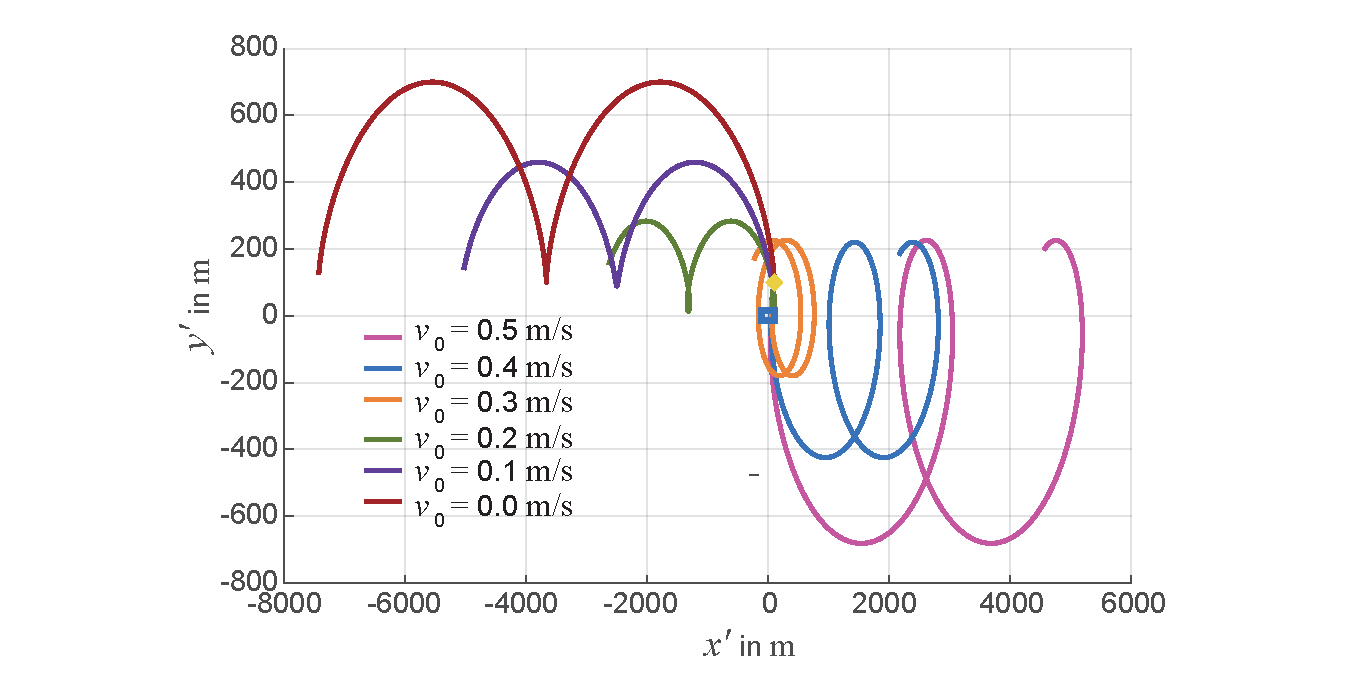
\includegraphics[width=\textwidth]{RendezvousAstronaut01.pdf} 
	%\caption[Astronaut au�erhalb der ISS.]{Astronaut au�erhalb der ISS. Der Astronaut befindet sich initial bei $x_0'=y_0'=\SI{100}{\metre}$ und bewegt sich mit einer Anfangsgeschwindigkeit $v_0$ (also keine initiale Relativgeschwindigkeit zum Ziel, d.h. $\dot{x}_0'=\dot{y}_0=0'$) genau in Richtung auf die Station zu. Selbst bei $v_0=0$ entfernt sich der Astronaut mit der Zeit von der Raumstation. Dargestellt sind die L�sungen der Clohessy-Wiltshire-Gleichungen wie im \mscr~ \mladynref{Rendezvous01.m} im Detail ausgef�hrt.}
	%\label{abb:adyn_rendezvous02}
%\end{figure}
%
  %\item[b)]
    %Was passiert, wenn der Astronaut seinen R�ckkehrantrieb (englisch \textit{Return-Thruster}) mit einem Antriebsverm�gen von $\SI{1}{\metre\per\second}$ einsetzt?   
		%Intuitiv \anf{zielt} der Astronaut mit seinem auf dem R�cksto�-Prinzip basierenden Thruster genau in Richtung ISS, also mit
    %\begin{align*}
        %\vec{v}_0 = 
        %\begin{pmatrix}
            %\dot{x}_0'\\
            %\dot{y}_0'\\
            %\dot{z}_0'
        %\end{pmatrix}
        %= \frac{1}{\sqrt{2}}
        %\begin{pmatrix}
            %1\\
            %1\\
            %0
        %\end{pmatrix}
        %\SI{}{\metre\per\second}\,.
    %\end{align*}
    %Leider wird durch die kombinierte Wirkung der Gezeiten und Coriolis-Kraft der Astronaut die ISS verfehlen, wie Gleichung \eqref{eq:adyn_rendez23} und \figref{adyn_rendezvous02} und \figref{adyn_rendezvous03}a zeigen.\\
    %\item[c)]
    %Wie muss der Astronaut beim Abfeuern seines Thrusters zielen, damit er die ISS sicher erreicht? \\
		%$\dot{x}_0'$, $\dot{y}_0'$ ergeben sich aus \eqref{eq:adyn_rendez24}. Wir k�nnen noch eine kleine Eigengeschwindigkeit des Astronauten vor dem Starten des Thrusters mit $\vec{v}_\text{vor} = \lk\dot{x}_{\text{vor},0'}, \dot{y}_{\text{vor},0'}\rk$ annehmen und erhalten den richtigen Zielwinkel:
    %\begin{align}
        %\tan\lk\gamma\rk = \frac{\Delta v_y}{\Delta v_x} = \frac{\dot{y}_0' -\dot{y}_{\text{vor},0'}}{\dot{x}_0'- \dot{x}_{\text{vor},0'}} \,. \label{eq:adyn_rendez27}
    %\end{align}
%\end{enumerate}
%In der Realit�t wird sich der Astronaut nat�rlich in kleinen Minisch�ben iterativ der ISS n�hern, doch auch daf�r gelten die abgeleiteten Formeln.
%
%\begin{figure}[H]
	%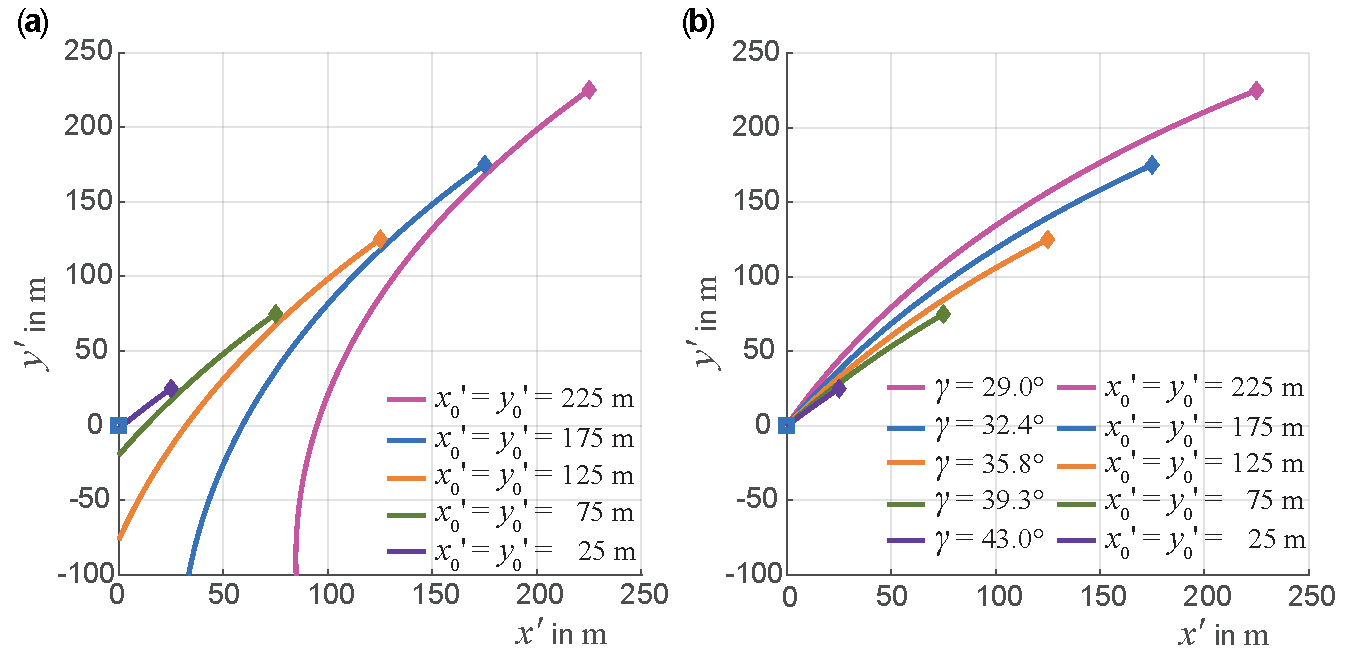
\includegraphics[width=\textwidth]{RendezvousAstronaut02.pdf} 
	%\caption[Astronaut au�erhalb der ISS.]{Astronaut au�erhalb der ISS. \fa Der Astronaut befindet sich initial bei $x_0'=y_0'=\SI{25}{\metre} \ldots \SI{225}{\metre}$ und "`zielt"' mit seinem Antriebssystem  mit einer Anfangsgeschwindigkeit $v_0$ genau in Richtung auf die Station. L�sung der Hill-Gleichungen. \fb Der Astronaut befindet sich ebenfalls initial bei $x_0'=y_0'=\SI{25}{\metre} \ldots \SI{225}{\metre}$ und bewegt sich mit einem optimierten Zielwinkel $\gamma$ der Richtung Anfangsgeschwindigkeit von $v_0 = \SI{1}{\metre\per\second}$ auf die Station zu (L�sung der Clohessy-Wiltshire-Gleichungen\index{Clohessy-Wiltshire-Gleichungen}). Offensichtlich wird der Astronaut erst bei Entfernung von kleiner als 50 m bei direkter Anzielung der Station auch bei dieser wirklich ankommen. Die Rechnungen sind im \mscr~ \mladynref{Rendezvous02.m} im Detail ausgef�hrt.}
	%\label{abb:adyn_rendezvous03}
%\end{figure}
%
%\label{bsp:adyn_stranded_astronaut}
%\end{example}
%
%

Wir verweisen auf die MATLAB-Skripte \mladynref{Rendezvous04.m} und \mladynref{Rendezvous05.m}.

\begin{figure}[H]
	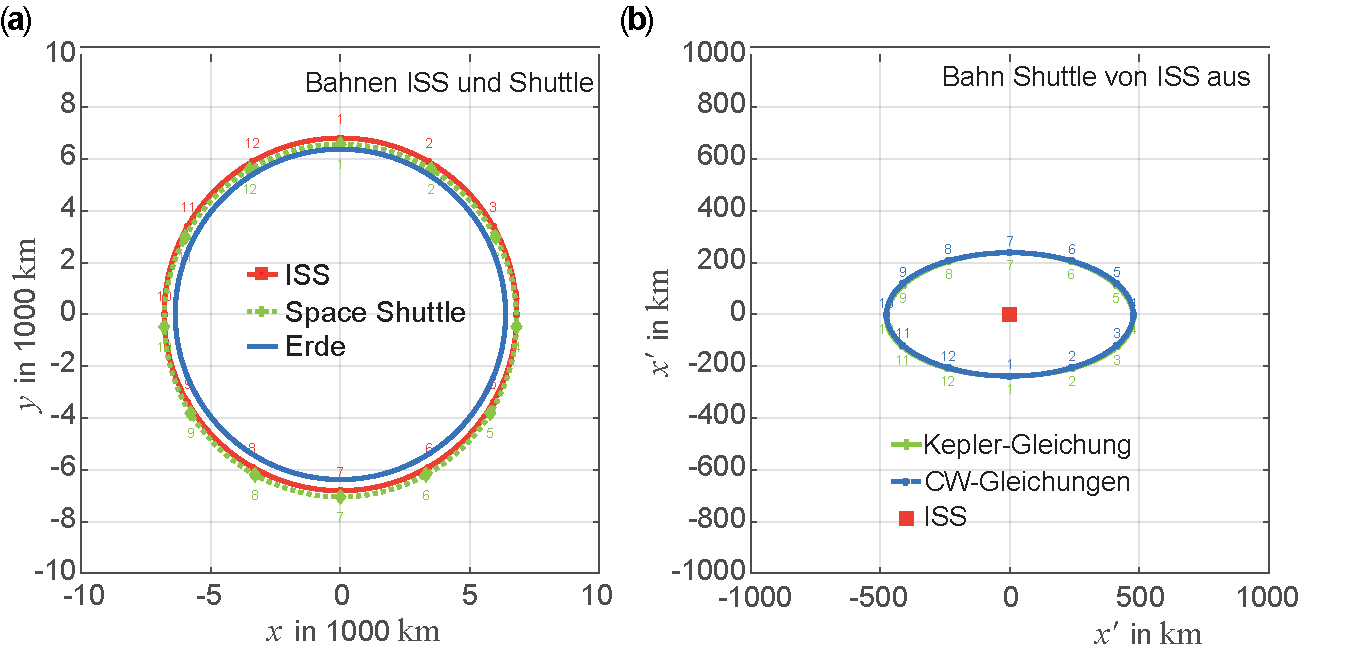
\includegraphics[width=\textwidth]{SpaceShuttle2ISS.pdf} 
	\caption[Space Shuttle und ISS in unterschiedlichen Umlaufbahnen.]{Space Shuttle und ISS in unterschiedlichen Umlaufbahnen. \fa Bahnen von ISS und Space Shuttle. Die Shuttle Bahn ist fiktiv, um das Prinzip zu erl�utern. In der Realit�t war die Shuttle Bahn viel n�her an der ISS. \fb Bahn Space Shuttle von ISS aus. L�sungen nach der Kepler-Gleichung mit Drehung des mitbewegten \KOS des Ziels und CW-L�sung im Vergleich. Die �bereinstimmung der exakten L�sungen nach der Kepler-Gleichung mit der CW-L�sung ist sehr gut, da auf Grund der Parameter die Linearisierungsbedingung f�r die CW-Gleichung relativ gut erf�llt ist.}
	\label{abb:adyn_rendezvous04Lsg}
\end{figure}

\end{sol} 
\textcolor{blue} {$\rightarrow$ zur} \probref{adyn_rendezvous01}.\\
\noindent\rule[1ex]{\textwidth}{0.5pt}  \newpage  \clearpage


%-----------------------------------------------------------------------------------------------------------

\begin{sol}{prob:adyn_rendezvous02}\label{lsg:adyn_rendezvous02} %�bung23
\textbf{Rendezvous Apollo 11 CSM und LM}\\

Die L�sung zum Rendezvous von LM und CSM von Apollo 11 in der Mondumlaufbahn ist im Detail im \mscr~\mladynref{LMCSMApollo11.m} als Berechnung der Kinematik des Rendezvous �ber die Clohessy-Wiltshire-Gleichungen ausgef�hrt. Wir erhalten die \figref{adyn_rendezvous06} aus \kap{adyn_rendezvous_apollo11}.\\

\begin{figure}[H]
	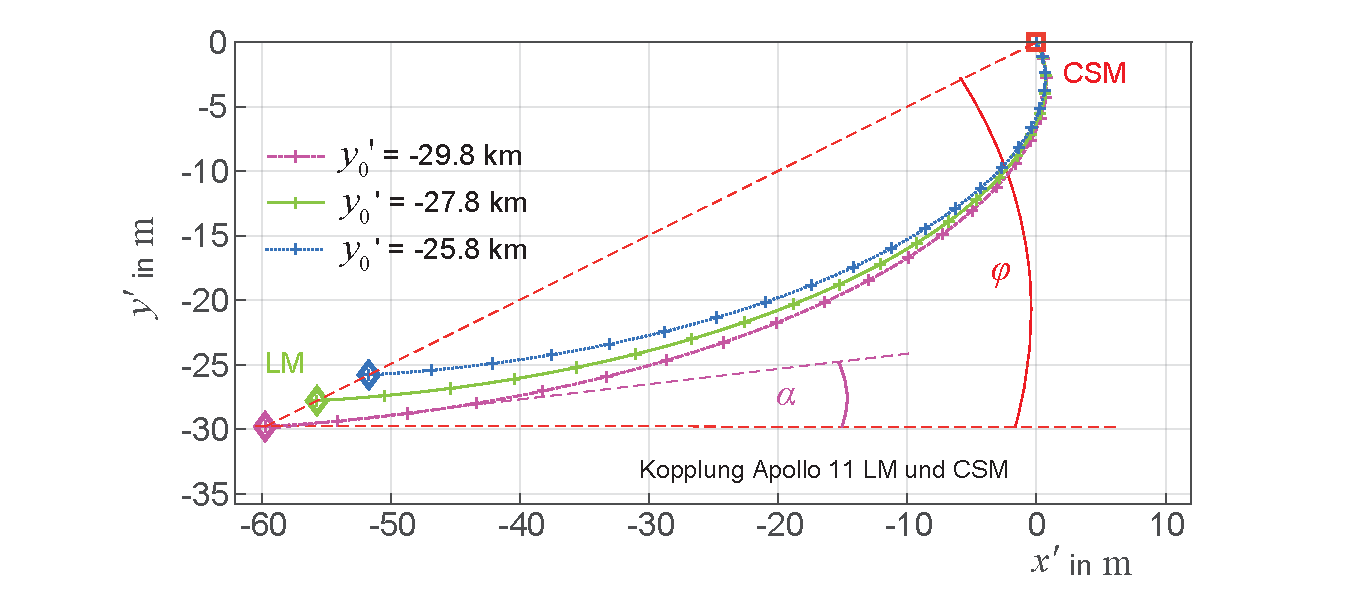
\includegraphics[width=\textwidth]{Apollo11LMCSMTrajektorie.pdf} 
	\caption[Trajektorien des LM im Anflug auf das CSM von Apollo 11.]{Trajektorien des LM im Anflug auf das CSM von Apollo 11 f�r verschiedene H�hen des TPI-Burn. Siehe \probref{adyn_rendezvous02} \bzw \mscr{}\mladynref{LMCSMApollo11.m}.}
	\label{abb:adyn_rendezvous06_uebung}
\end{figure}

\end{sol} 
\textcolor{blue} {$\rightarrow$ zur} \probref{adyn_rendezvous02}.\\
\noindent\rule[1ex]{\textwidth}{0.5pt} \newpage \clearpage 

%-----------------------------------------------------------------------------------------------------------

\begin{sol}{prob:adyn_rendezvous03}\label{lsg:adyn_rendezvous03} %�bung24
\textbf{Planung einer Apollo Mission - \textit{Free Return Trajectory}}\\

\begin{subprobs}
\subprob{Absch�tzungen}
Wir wollen als erstes eine Absch�tzung f�r die Flugzeit zum Mond treffen und nehmen dabei eine koplanare Bewegung von Flugbahn und Mondbahn an, letztere wird auch noch als Kreisbahn angenommen (\figref{adyn_FRT01}).\\
Der Punkt $\mathrm{P}_0$ (Abstand $r_0$ vom Erdzentrum) in der Parkbahn um die Erde, aus der der Einschuss (Injektion) in die translunare Bahn erfolgt, wird \textit{(Translunar Injection Point} (TLI) genannt. Dort gilt f�r die Energie und den Drehimpuls des Raumschiffs bezogen auf das Erd-\KOS:
\begin{align}
H_0 = \frac{v_0{}^2}{2} - \frac{\mu_\text{E}}{r_0}\,, & L_0 = r_0\,v_0\,\cos\gamma_0\,. \label{eq:adyn_lsg_FRT01}
\end{align}
Hierin sind $v_0\,\cos\gamma_0$ die Komponente der Raumschiff-Geschwindigkeit in Richtung lokaler Horizont mit $\gamma_0$ als der FPA bei $r_0$.\\
Damit ergeben sich f�r die Ellipse zum Mond folgende Ellipsenparameter (vergleiche auch Gleichungen \eqref{eq:hm_bewgl1} und \eqref{eq:hm_relations1}):
\begin{align}
\begin{split}
    p &= \frac{L_0{}^2}{\mu_ \text{E}}\,,~~~~ a = -\frac{\mu_\text{E}}{2H_0}\,, ~~~~
    e = \sqrt{1 - \frac{p}{a}} \,=\, \sqrt{1+\frac{L_0{}^2}{\mu_\text{E}{}^2}\,2H_0}\,~.
\end{split} \label{eq:adyn_lsg_FRT02}
\end{align}
\begin{figure}[H]
	\includegraphics[width=\textwidth]{Transfer2Moon.pdf} 
	\caption[Geometrie des Flugs zum Mond.]{Vereinfachte Geometrie des Flugs eines Raumschiffes zum Mond. Im Bild wurde eine koplanare Bewegung von Raumschiff und Mond in der Ekliptik angenommen (Draufsicht auf die Ekliptik). (Nach \cite{Bate1971}).}
	\label{abb:adyn_FRT01}
\end{figure}

In \figref{adyn_FRT01} definieren wir aus der Geometrie f�r die weitere mathematische Behandlung folgende Parameter:
\begin{align*} 
    r_0 && &\text{geozentrischer Abstand des Raumschiffs bei Injektion in die translunare Bahn} \\
    r_1 && &\text{geozentrischer Abstand des Raumschiffs beim Erreichen der SOI des Mondes}\\
    && &r_1 = \sqrt{r_{\text{EM}}{}^2 + R_{\text{SOI, M}}{}^2 - 2 r_{\text{EM}} R_{\text{SOI, M}} \cos\gamma_1} \\
    r_\text{EM} && &\text{Abstand der Massezentren von Erde und Mond}      \\
    R_\text{SOI,M} && &\text{Radius der SOI des Mondes}\\
    \varphi_0 && &\text{geozentrischer Phasenwinkel des Mondes bei Abflug (TLI) relativ zur}\\
    && &\text{Verbindungslinie Erde/Raumschiff}\\
    \varphi_1 && &\text{geozentrischer Phasenwinkel des Mondes bei Ankunft des Raumschiffs }\\
    && &\text{an der SOI relativ zur Verbindungslinie Erde/Raumschiff}\\
    \lambda_1 && &\text{selenozentrischer Winkel zwischen Ankunftsort des Raumschiffs}\\
    && &\text{an der SOI des Mondes und der Verbindungslinie Erde/Mond}\\
    \gamma_0,\gamma_1 && &\text{FPA des Raumschiffs bei TLI \bzw Ankunft an der SOI des Mondes}\\
    \upsilon_0,\upsilon_1 && &\text{wahre Anomalien der Ellipsenbahn bei TLI \bzw Ankunft SOI des Mondes}\\
    \omega_\text{M} && &\text{Umlaufgeschwindigkeit des Mondes}\,\approx \SI{2.649e-6}{\radian\per\second}\\
		a, e, P && &\text{Parameter der Transferellipse zum Mond}
\end{align*}
F�r eine Planung eines Fluges zum Mond startet man mit Vorgaben f�r $r_0,\,v_0,\,\gamma_0$ und $\lambda_1$ und berechnet die Flugzeit $t_\text{F} = \mathrm{ToF}$,\;$\varphi_0$,\, $\varphi_1$ und $\gamma_1$. Ergeben sich daraus keine sinnvollen Werte, so muss man $r_0,\,v_0,\,\gamma_0$ und $\lambda_1$ variieren. \\
Aus den Ellipsenparametern $a$, $p$, $e$ lassen sich nun bei bekannten $r_0,r_1$ die jeweiligen wahren Anomalien berechnen.
\begin{align}
\begin{split}
    \cos\upsilon_0 &= \frac{p - r_0}{\e\,r_0} \,,\\
    \cos \upsilon_1 &= \frac{p - r_1}{\e \,r_1} \quad \text{mit} \quad r_1 = \sqrt{r_{\text{EM}}{}^2 + R_{\text{SOI,M}}{}^2 - 2 r_{\text{EM}}\,R_{\text{SOI,M}} \cos \lambda_1}
\end{split}\label{eq:adyn_lsg_FRT03}
\end{align}
Die Flugzeit zum Mond ergibt sich �ber die Kepler-Gleichung zu:
\begin{align}
    t_\text{F} = t_1 - t_0 = \lk\sqrt{\frac{a^3}{\mu_\text{E}}}\rk \lek E_1 - E_0 - \e\,\lk \sin E_1 - \sin E_0\rk\rek\label{eq:adyn_lsg_FRT04}
\end{align}
wobei sich die exzentrische Anomalien $E_i~~(i=1,2)$ entweder aus
\begin{align}
\begin{split}
    \cos E_i &= \frac{\e - \cos \upsilon_i}{1 + \e \cos \upsilon_i} = \lk 1 - \frac{r_i}{a}\rk\,\frac{1}{\e}\\
    \text{oder}\quad \tan \frac{E_i}{2} &= \sqrt{\frac{1-\e}{1+\e}}\,\tan \lk \frac{\upsilon_i}{2} \rk    
\end{split}\label{eq:adyn_lsg_FRT05}
\end{align}
ergeben (\vgl Gleichungen \eqref{eq:hm_r_param_ellipse} und \eqref{eq:hm_nu(t)_alternativ}).\\
Wir brauchen noch den Winkel $\varphi_1$, dieser ergibt sich nach dem Sinussatz aus
\begin{align}
    \sin\varphi_1 = \frac{R_{\text{SOI,M}}}{r_1}\,\sin\lambda_1 \,. \label{eq:adyn_lsg_FRT06}
\end{align}
F�r eine Absch�tzung der Flugzeiten wollen wir annehmen, dass $\gamma_0 \approx 0$ ist. Wir k�nnen dann die Flugzeiten f�r verschiedene $\lambda_1$ \bzw $\varphi_1$ als Funktion der TLI-Geschwindigkeit $v_0$ berechnen.

\begin{figure}[H]
	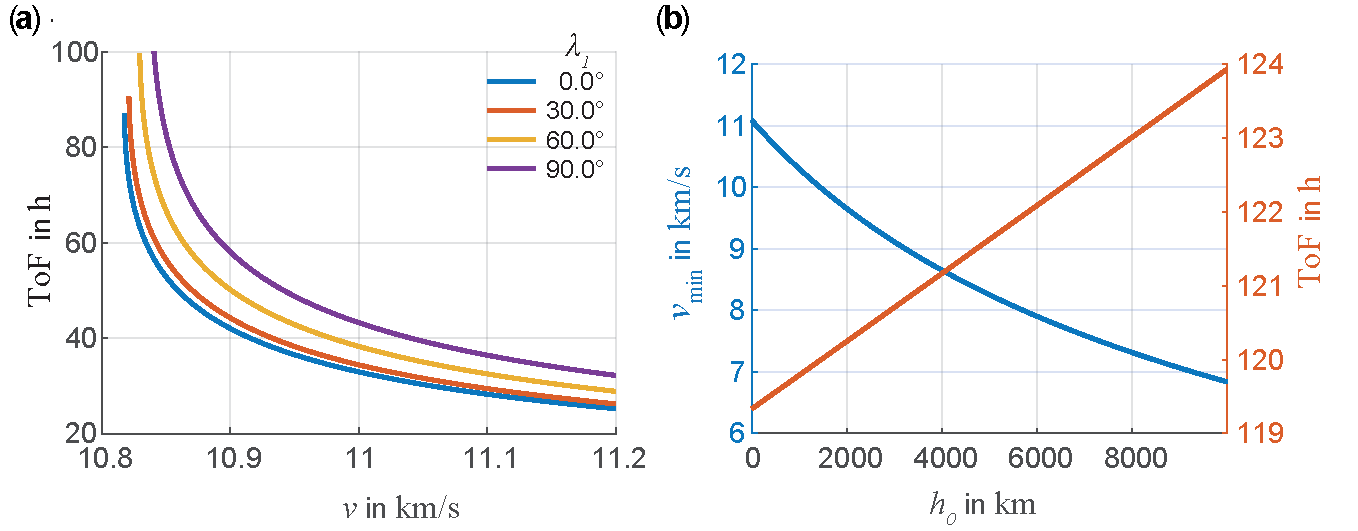
\includegraphics[width=\textwidth]{Transfer2MoonTOF.pdf} 
	\caption[Flugzeiten und Minimalgeschwindigkeit zum Mond.]{Flugzeiten und Minimalgeschwindigkeit zum Mond. \fa ToF als Funktion der TLI-Geschwindigkeit $v_0$ \fb Minimum-Geschwindigkeit $v_\text{min}$ f�r TLI und zugeh�rige ToF als Funktion des Radius $r_0$ der erdnahen Kreisbahn. Siehe \mscr~\mladynref{Transfer2Moon.m}.}
	\label{abb:adyn_FRT02}
\end{figure}

Man erkennt aus \figref{adyn_FRT02}a, dass es eine minimale Geschwindigkeit $v_{\text{min}}$ (abh�ngig vom Winkel $\lambda_1$) gibt, um �berhaupt in endlicher Zeit den Mond zu erreichen. Diese liegt bei etwas �ber $\SI{10.8}{\km\per\second}$ f�r $\lambda_1 =0$ und ist ebenfalls abh�ngig und der H�he $h_0$ der Parkbahn in Erdn�he.\\
Man kann nun eine einfache numerische Absch�tzung f�r $v_{\text{min}}$ machen, wenn man annimmt, dass die TLI am Perig�um erfolgen soll.
Dann ist definitiv $\gamma_0 = 0$ und das Apog�um der elliptischen translunaren Bahn entspricht dann $r_{\text{EM}}$ (\bzw $r_{\text{EM}} - R_{\text{SOI,M}}$, wenn wir die SOI ber�cksichtigen wollen). Wir finden also:
\begin{align}
     2a_0 &= r_0 + r_{\text{EM}} ~~~\text{und}~~~H_0 = -\frac{\mu_\text{E}}{2a} = \frac{v_{\text{min}}{}^2}{2} - \frac{\mu_\text{E}}{r_0} \nonumber \\
    \rightarrow \quad v_{\text{min}}{}^2 &= \frac{2\mu_\text{E}}{r_0}\,\lk 1 - \frac{1}{1 + r_{\text{EM}}/r_0}\rk ~~ \text{und} ~~~ \text{ToF}_{\text{max}} = \pi \sqrt{\frac{a_0{}^3}{\mu_\text{E}}} \,. \label{eq:adyn_lsg_FRT07}
\end{align}
Man erh�lt dann \zb f�r $h_0 = \SI{400}{\km}$ eine minimale notwendige Geschwindigkeit von $v_{\text{min}} = \SI{10.75}{\km\per\second}$ und eine (maximale) Flugzeit von $ \text{ToF}_{\text{max}} = \SI{119.5}{\hour}$ (\figref{adyn_FRT03}), 
was wesentlich l�nger ist, als \zb Apollo 11 zum Mond brauchte.\\
Man erkennt sehr sch�n aus \figref{adyn_FRT02}, wie kleine �nderungen der TLI-Anfangsgeschwindigkeit die Flugzeit wesentlich verk�rzen.

\subprob {\textit{Patch Conic} - N�herung}

Nach diesen grunds�tzlichen �berlegungen wollen wir nun die Bahn genauer berechnen und dabei das Konzept der SOI (siehe \kap{adyn_gravity_assist} \bzw \probref{adyn_SOI}) benutzen. Bisher haben wir ja die Gravitationswirkung des Mondes vernachl�ssigt. Wir arbeiten in den relevanten Bereichen jeweils nur mit der SOI der Erde \bzw des Mondes. Dies f�hrt auf das sogenannte Konzept der \textit{Patched Conic} (der "`aneinandergest�ckelten Kegelschnitte"', \vgl auch \probref{adyn_SOI}). 

\begin{figure}[H]
	\includegraphics[width=\textwidth]{Transfer2MoonPP.pdf} 
	\caption[Geometrie des Transfers zum Mond am \textit{Patch Point}.]{Geometrie des Transfers zum Mond am \textit{Patch Point}. Die Koordinaten im selenozentrischen \KOS werden mit dem Index 2 bezeichnet und sind in rot gezeichnet. Der Winkel $\varepsilon_2$ bezeichnet den anf�nglichen selenozentrischen Winkel der Geschwindigkeit des Raumschiffs relativ zum Mondzentrum. (Nach \cite{Bate1971}.)}
	\label{abb:adyn_FRT03}
\end{figure}

Wir berechnen zun�chst die Transferphase vom TLI bis zum Erreichen der SOI des Mondes. Dazu berechnen wir �ber \eqref{eq:adyn_lsg_FRT03}-\eqref{eq:adyn_lsg_FRT05} die ToF und auch den geozentrischen Phasenwinkel $\varphi_0$, den der Mond bei der TLI haben muss:
\begin{align}
    \varphi_0 = \upsilon_1 - \upsilon_0 - \gamma_1 - \omega_{\text{M}}\,  \lk t_1 - t_0\rk\,. \label{eq:adyn_lsg_FRT08}
\end{align}
Wir schauen uns nun genauer die Bedingungen am sogenannten \textit{Patch Point}, dem Punkt PP an. Wir bestimmen dort zun�chst die Geschwindigkeit $\vec{v}_2$ des Raumschiffs im selenozentrischen (\dh lunaren) \KOS:
\begin{align}
\begin{split}
    \vec{v}_2 &= -\vec{v}_{\text{M}} + \vec{v}_1\\
    v_2 &= \sqrt{v_1{}^2 + v_{\text{M}}{}^2 - 2 v_1\,v_{\text{M}}\,\cos \lk \gamma_1 - \varphi_1\rk} 
\end{split}\label{eq:adyn_lsg_FRT09}
\end{align}
mit
\begin{align*}
    v_{\text{M}} = \omega_{\text{M}}\,r_{\text{EM}} \approx \SI{1.018}{\km\per\second}.
\end{align*}
Ferner gilt am Punkt PP $r_2 = R_{\text{SOI,M}}$ und 
\begin{align}
    \varepsilon_2 = \arcsin \lk\frac{v_\text{M}}{v_2}\,\cos\lambda_1 - \frac{v_1}{v_2}\,\cos\lk \lambda_1 + \varphi_1-\gamma_1\rk\rk \,. \label{eq:adyn_lsg_FRT10}
\end{align}
Letztere Beziehung kann man sich ebenfalls aus \figref{adyn_FRT03} �ber
\begin{align*}
    v_2\,\sin\epsilon_2 = v_{\text{M}}\,\cos \lambda_1 - v_1\,\cos\lk\lambda_1 + \varphi_1 - \gamma_1\rk
\end{align*}
herleiten. F�r eine direkte Landung auf dem Mond muss der Winkel $\varepsilon_2$ logischerweise $0$ sein. 
F�r alle anderen F�lle kann man nun mit den \anf{lunaren} Anfangsbedingungen $r_2$, $v_2$ und $\epsilon_2$ drei m�gliche Trajektorien um den Mond herum unterscheiden:
\begin{enumerate}
    \item [1)] Aufschlag auf den Mond: In diesem Fall ist das Periselenium $r_{\text{P,M}}$ (kleinster Abstand der Bahn vom Mondzentrum) kleiner als der Mondradius $R_{\text{M}}$.
    \item [2)] Mondumlaufbahn, \dh Einschwenken auf eine Mondumlaufbahn durch Abbremsen/Beschleunigen auf die notwendige Umlaufgeschwindigkeit  $v_3$.
    \item [3)] Mondumrundung (\zb als \textit{Free Return Trajektory} (FRT)), wobei besonders das Periselenium und die Bedingungen ($r_3$, $v_3$, $\gamma_3$, $\lambda_3$) beim Verlassen der SOI des Mondes interessant sind, da diese in ma�gebliche die R�ckkehrbahn zur Erde bestimmen.
\end{enumerate}
Wir m�ssen daher als n�chstes das Periselenium $r_\text{P,M}$ berechnen, da wir das ja in jedem der drei F�lle zur Bewertung der Bahn um den Mond brauchen. In der SOI des Mondes gilt im \KOS des Mondes gilt nat�rlich wieder Energie- und Drehimpulserhaltung:
\begin{align}
\begin{split}
    H_2 &= \frac{v_2{}^2}{2} - \frac{\mu_\text{M}}{r_2}\,~~\text{mit}~~ \mu_ \text{M} = G\,M_\text{M} \,\\
		L_2 &=  r_2 \, v_2\,\cos \gamma_2 = r_2\,v_2\,\sin \varepsilon_2 \,, ~~\text{da}~~ \gamma_2 = 90^\degree - \varepsilon_2\,.
\end{split}\label{eq:adyn_lsg_FRT11}
\end{align}
Wie bei der Berechnung der Transferellipse finden wir die Kegelschnittparameter\footnote{Der Kegelschnitt wird \ia eine Hyperbel sein.} f�r die Mondbahn:
\begin{align}
    p_2 = \frac{L^2}{\mu_\text{M}}\,, \quad e_2 = \sqrt{1 + \frac{2 H_2\,L^2}{\mu_\text{M}{}^2}} \label{eq:adyn_lsg_FRT12}
\end{align}
und daraus
\begin{align}
    r_\text{P,M} = \frac{p_2}{1 + \e}\,, \quad v_\text{P,M} = \sqrt{2 \lk H_2 + \frac{\mu_\text{M}}{r_\text{P,M}} \rk} \label{eq:adyn_lsg_FRT13}
\end{align}
Wir wollen als Beispiel durchrechnen:
\begin{align*}
    r_0 &= \SI{300}{\km} + R_\text{E} = \SI{6678}{\km}\,,~~
    v_0 = \SI{10.87}{\km\per\second}\,,~~
    \gamma_0 = 0^\degree\,,~~
    \lambda_1 = 30^\degree\,.
\end{align*}
Ohne weitere Kurskorrekturen wird die geringste Entfernung zur Mondoberfl�che
\begin{align*}
    h_\text{P,M} = r_\text{P,M} - R_\text{M} = r_\text{P,M} - \SI{1737.4}{\km} = \SI{1413.6}{\km}\,.
\end{align*}
Wie bereits erw�hnt, kommt es f�r  $h_\text{P,M} < 0$ zur Landung \bzw zum Aufschlag auf dem Mond, abh�ngig von $v\lk h_\text{M} = 0\rk$ und je nach Verf�gbarkeit von Bremsm�glichkeiten.\\

\begin{figure}[H]
	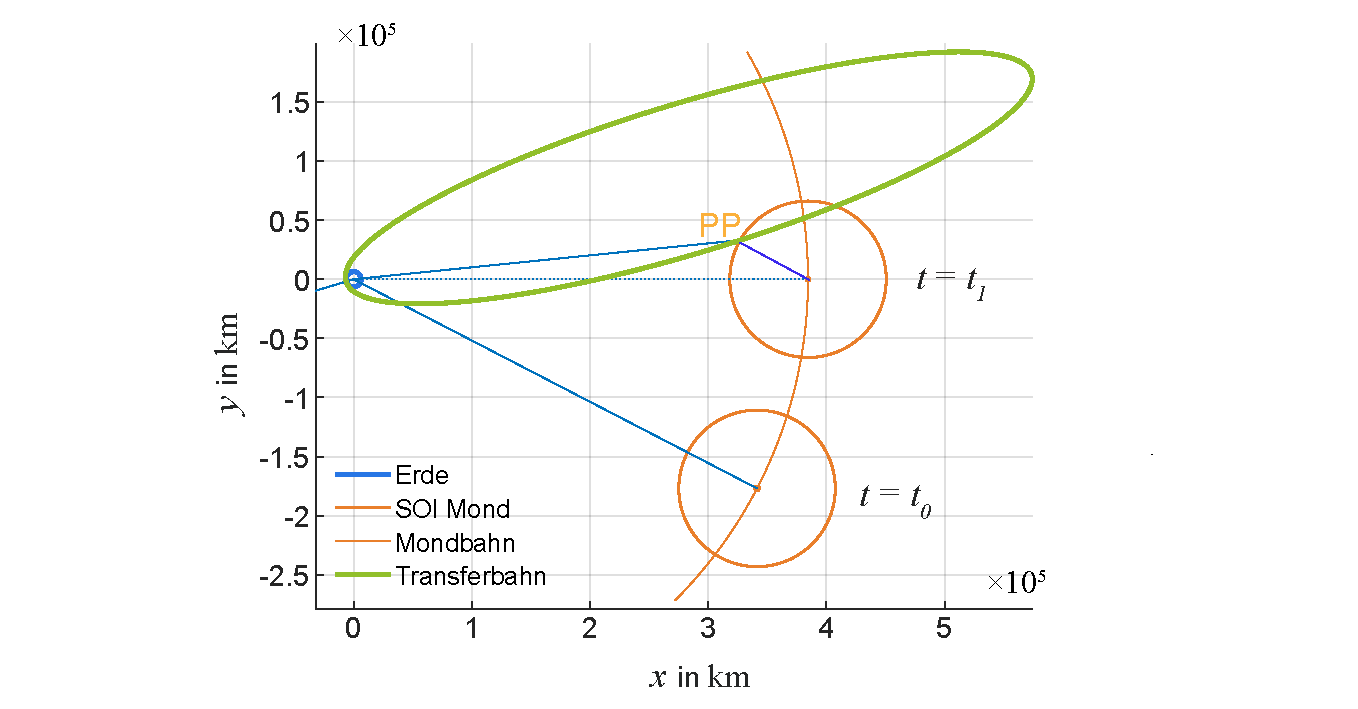
\includegraphics[width=\textwidth]{Transfer2Moon04.pdf} 
	\caption[Berechnete Geometrie des Transfers zum Mond.]{Berechnete Geometrie des Transfers eines Raumschiffes zum Mond. In der Rechnung wurde eine koplanare Bewegung von Raumschiff und Mond in der Ekliptik angenommen. Parameter siehe Tabelle \ref{tab:adyn_FRT01} und \mscr~\mladynref{Transfer2MoonExample.m}.}
	\label{abb:adyn_FRT04}
\end{figure}


Die Parameter f�r die \figref{adyn_FRT04} und \figref{adyn_FRT05} sind in folgender Tabelle gelistet:
\begin{table}[h!]
\centering
\begin{tabular}{|c|c|c|c|c|c|}
\hline
\multicolumn{6}{|l|}{\textbf{Vorgaben und Abflugparameter @TLI}} \\
\hline
$h_0$ (km) & $\gamma_0$ ($\degree$) & $v_0$ (km/s) & $\lambda_1$ ($\degree$) & &   \\
\hline
300.0 & 0.0 & 10.87 & 30.0 & &  \\
\hline
\multicolumn{6}{|l|}{\textbf{Abflugparameter @TLI}} \\
\hline
$a_0$ (km) & $p_0$ (km) & $\e_0$  & $\phi_0$ ($\degree$) &  &  \\
\hline
$\SI{3.03e5}{}$& $\SI{1.32e4}{}$& 0.9780 & 135.77 & &   \\
\hline
\multicolumn{6}{|l|}{\textbf{Parameter auf Transfer zum Mond}} \\
\hline
$v_1$ (km/s) & $v_2$ (km/s) & $\upsilon_1$ &$\upsilon_2$ & $\mathrm{TOF}$ (h) &  \\
\hline
1.054 & 1.220 &0.0 & 5.78 & 50.15&  \\
\hline
\multicolumn{6}{|l|}{\textbf{Parameter am Mond}} \\
\hline
$r_2$ (km) & $\epsilon_2$ ($\degree$) & $p_2$ (km) &$\e_2$ & $h_\text{PM}$ (km)& $\mathrm{TOF}_\text{SOI}$ (h)  \\
\hline
$\SI{6.62e4}{}$ & 4.72 & 9014.8 & 1.8610 & 1413.6 & 28.05 \\
\hline
\end{tabular}
\caption{Parameter f�r \textit{Patch Conic} N�herung} \label{tab:adyn_FRT01}
\end{table}
Hierin ist $\mathrm{TOF}$ die Flugzeit von der TLI bis zum Erreichen der SOI des Mondes und $\mathrm{TOF}_\text{SOI}$ die Flugzeit zum Durchfliegen der SOI des Mondes. \\
Insgesamt ergibt sich f�r einen Flug bis zur R�ckseite des Mondes eine Gesamtflugzeit von
\begin{align*}
    t_\text{F} = \mathrm{TOF} + \frac{1}{2} \mathrm{TOF}_\text{SOI} = \SI{50.15}{\hour} + \SI{14.025}{\hour} \approx \SI{64.175}{\hour}\,,
\end{align*}
also etwa weniger als 3 Tage und damit auch etwas schneller als Apollo 8 unterwegs war.\\

\begin{figure}[H]
	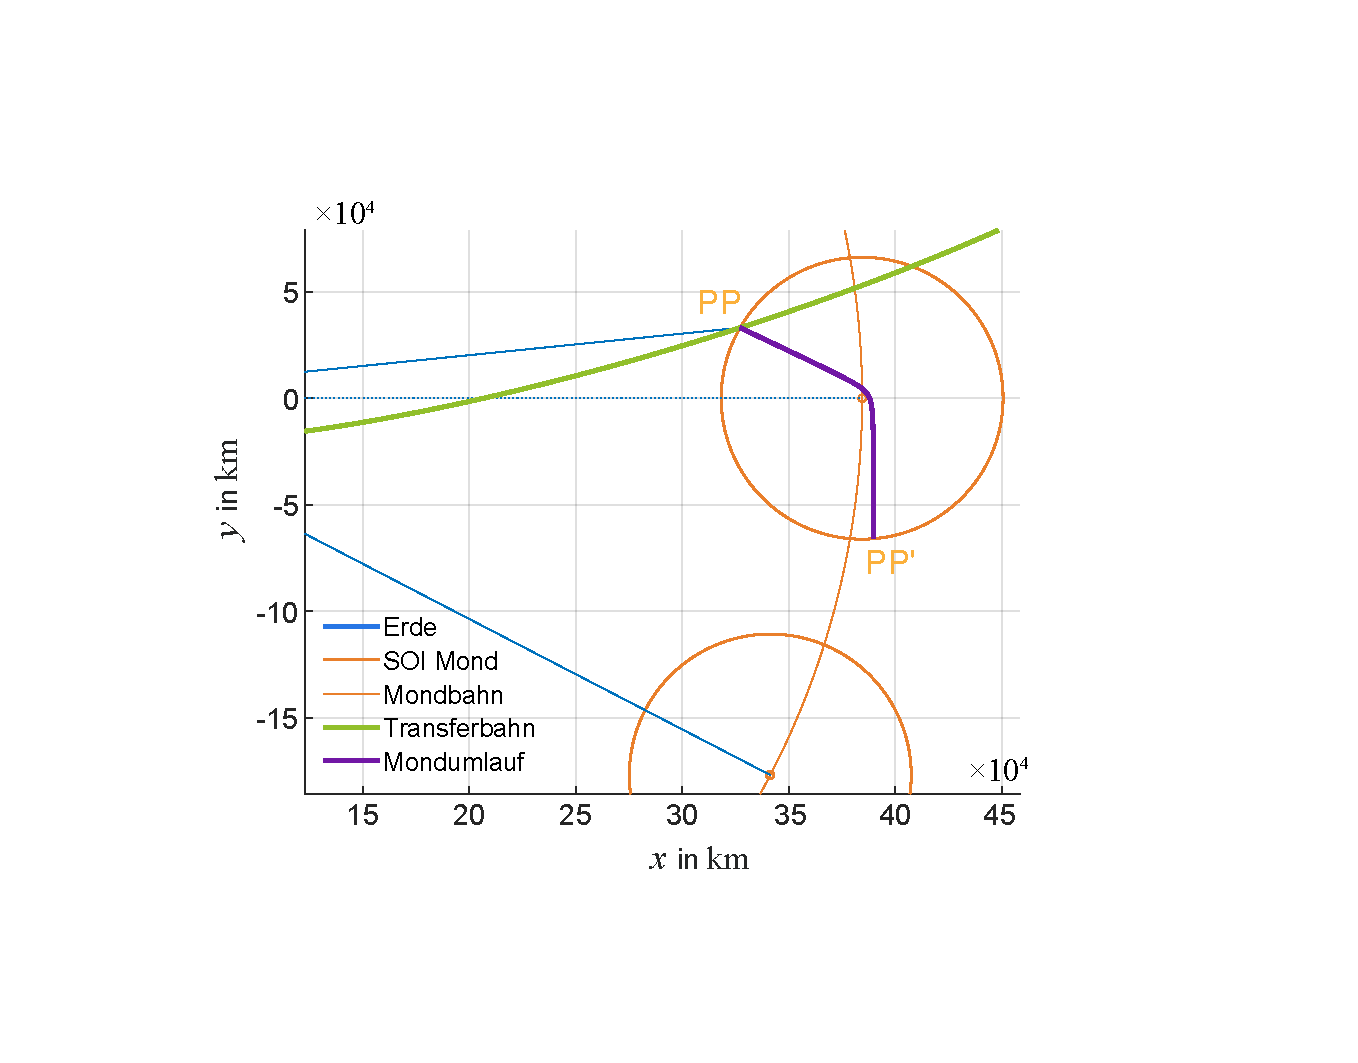
\includegraphics[width=\textwidth]{Transfer2Moon05.pdf} 
	\caption[Berechnete Geometrie des Transfers zum Mond am \textit{Patch Point}.]{Berechnete Geometrie des Transfers zum Mond am \textit{Patch Point}, sowie Mondumlauf. Die lila Kurve zeigt die Bahn des Raumschiffs im \KOS des Mondes. In der Rechnung wurde eine koplanare Bewegung von Raumschiff und Mond in der Ekliptik angenommen. Parameter siehe Tabelle Parameter siehe Tabelle \ref{tab:adyn_FRT01} und \mscr~\mladynref{Transfer2MoonExample.m}. Man beachte, dass \figref{adyn_FRT05} die Bewegung im \KOS des Mondes zeigt und nicht im als Inertialsystem angenommenen geozentrischen \KOS der Erde. F�r eine Energie $H_2 > 0$ wird $\e_2 > 1$ und damit die Bewegung um den Mond eine Hyperbel. Man �berlege sich Analogien zur Behandlung des Gravity-Assist-Man�vers in \kap{adyn_gravity_assist}.}
	\label{abb:adyn_FRT05}
\end{figure}

Man kann die Werte am Punkt PP' berechnen und dann weiter transformieren in das Erd-\KOS, um zu sehen, ob eine \textit{Free Return Trajectory} vorliegt, ganz analog wie beim Swing-By-Man�ver.\\
Wir wollen jedoch im Folgenden die Rechnungen komplett, also auch die Bewegung um den Mond herum im Inertialsystem numerisch machen und k�nnen dabei als Startwert die Parameter der \textit{Patch Conic}-Rechnung �bernehmen.

\newpage
\subprob{Numerische Rechnung Vergleich \textit{Patch Conic} und 1. N�herung}

Wir wollen nun konkret den Raumflug von Apollo 13 anschauen und w�hlen  entsprechend des NASA Flight Journal (\url{https://www.nasa.gov/history/afj/ap13fj/index.html}) $h_0=\SI{169.609}{\km}$. Ebenso benutzen die Ergebnisse der \textit{Patch Conic} N�herung (\figref{adyn_FRT06}) als Startwerte f�r die numerische Rechnung und betrachten zun�chst die Erde als ruhend und den Mond auf einer Kreisbahn umlaufend. 

\begin{figure}[H]
	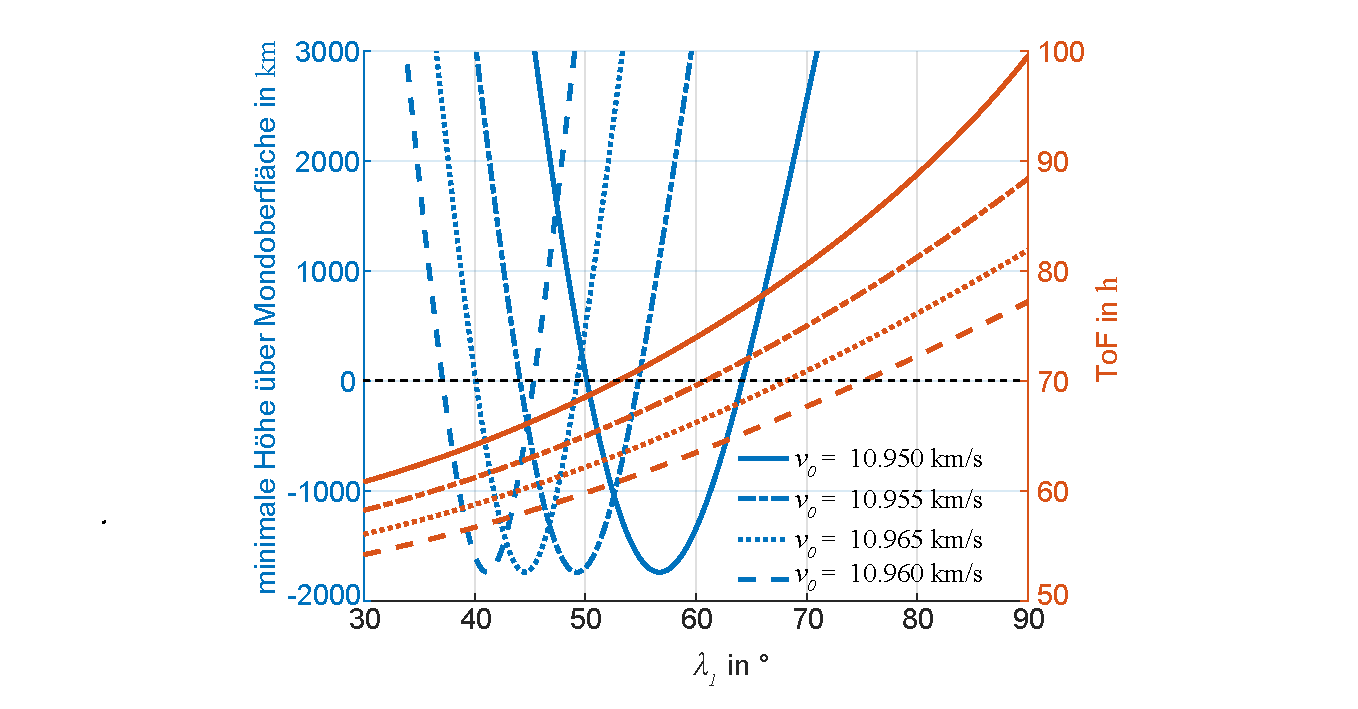
\includegraphics[width=\textwidth]{PatchConicApollo13.pdf} 
	\caption[Ergebnisse der \textit{Patch Conic} N�herung f�r Apollo 13.]{Ergebnisse der \textit{Patch Conic} N�herung f�r Apollo 13.}
	\label{abb:adyn_FRT06}
\end{figure}

Wir erhalten dann \zb f�r $v_0 = \SI{10960.0}{\km\per\second}$ in der
\textit{Patch Conic} N�herung:\\
\begin{align*}
	\lambda_1      &: 49.70\degree  && \\ 
	\varphi_0      &: 129.89\degree\\ 
	\mathrm{ToF} &: 78.7\,\mathrm{h}\\ 
	h_\text{P,M} &: \SI{279.3}{\km} \, 
\end{align*}
was schon relativ gut mit den tats�chlichen Werten von Apollo 13 �bereinstimmt, wobei man ber�cksichtigen muss, dass beim tats�chlichen Raumflug es eine Reihe von Kurskorrekturen gab.

In der numerische Betrachtung (L�sung der Bewegungsgleichungen) ergeben sich dann eine Vielzahl von L�sungen. Das liegt daran, dass es sich bei der Bestimmung der FRT ja um ein Optimierungsproblem handelt, bei dem $h_0$, $h_\text{Reentry}$ und $h_\text{P,M}$ gegeben sind und $v_0$ und $\varphi_0$ gesucht werden. F�r solche Optimierungsprobleme gibt es h�ufig keine eindeutigen L�sungen. Wir erhalten \zb f�r $v_0 = \SI{10960.0}{\km\per\second}$ und $\varphi_0 = 129.33\degree$:
\begin{align*}
	\mathrm{ToF}\, \text{zum Mond} &: 78.2\,\mathrm{h}\\ 
	\mathrm{ToF}\, \text{Gesamt} &: 156.4\,\mathrm{h}\\ 
	h_\text{M,P}\, \text{Mond} &: \SI{2111.0}{\km}\\
	h_\text{Reentry}\, \text{Erde} &: \SI{150.0}{\km} 
\end{align*}
Die L�sung ist im Detail im \mscr~\mladynref{FreeReturnTrajectoryApollo13.m} ausgef�hrt.\\

\subprob{Genauere Rechnungen f�r Apollo 13}

Bisher haben wir die Erde als ruhend angenommen und den Mond auf einer Kreisbahn um diese rotierend, Wir betrachten nun das vollst�ndige Dreik�rper-Problem Erde, Mond und Apollo 13 im Schwerpunktsystem von Erde-Mond. Wiederum handelt sich hierbei um ein Optimierungsproblem, bei dem $h_0$ und $h_\text{Reentry}$ gegeben sein sollen und $v_0$, $\varphi_0$ und $h_\text{P,M}$ gesucht werden.
Die Rechnungen ergeben in diesem Fall beispielhaft, 
\begin{align*}
	v_0      &: \SI{10963.0}{\km\per\second}\\ 
	\varphi_0      &: 130.46\degree\\ 
	\mathrm{ToF}\, \text{zum Mond} &: 75.2\,\mathrm{h}\\ 
	\mathrm{ToF}\, \text{Gesamt} &: 149.5\,\mathrm{h}\\ 
	h_\text{P,M}\, \text{Mond} &: \SI{1353.4}{\km}\\
	h_\text{Reentry}\, \text{Erde} &: \SI{169.6}{\km} \,,
\end{align*}
wobei wir hier vor darauf geachtet haben, dass der Wiedereintritt in die Erdatmosph�re gew�hrleistet ist, daf�r der Mondabstand etwas gr��er gew�hlt ist.
Das L�sungsbeispiel ist in \figref{adyn_FRT08} dargestellt und im Detail im \mscr~\mladynref{FreeReturnTrajectoryApollo13CoM.m} ausgef�hrt.\\

\begin{figure}[H]
	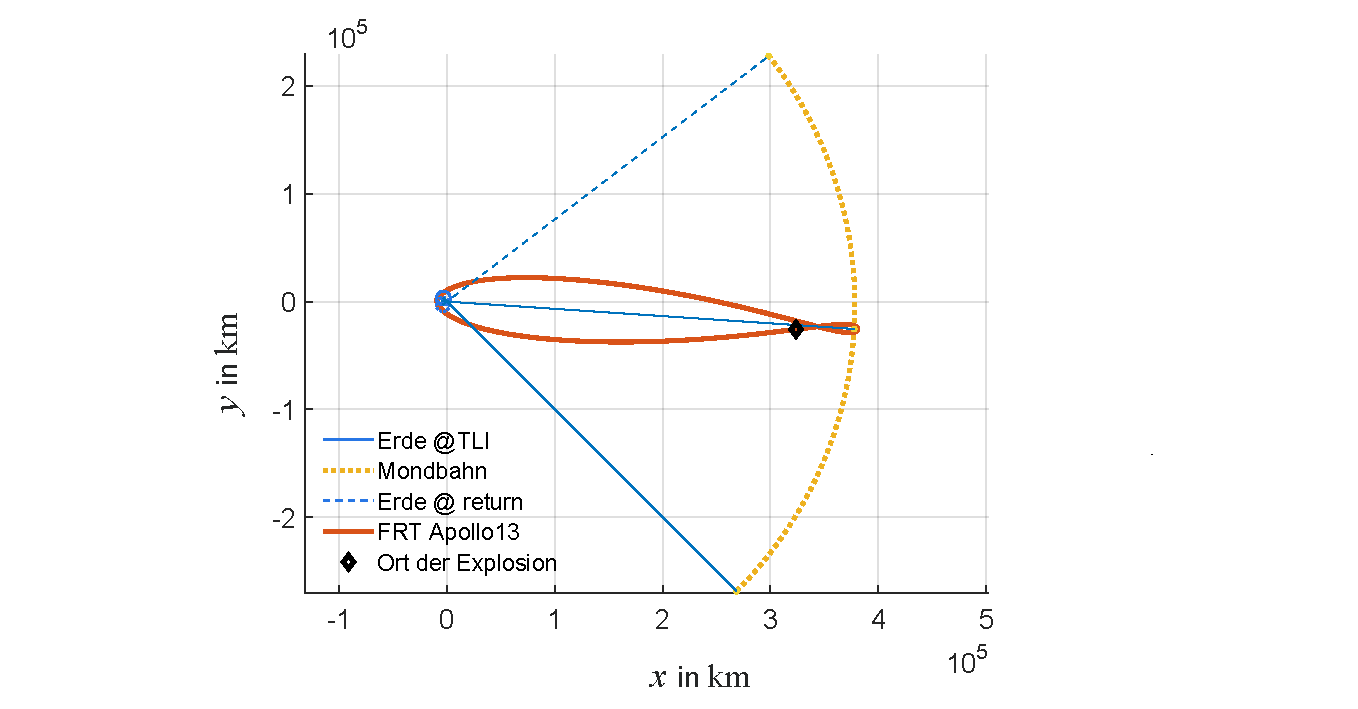
\includegraphics[width=\textwidth]{FRTApollo13.pdf} 
	\caption[Ergebnisse der numerischen Rechnung f�r eine \textit{Free Return Trajectory } f�r Apollo 13.]{Ergebnisse der numerischen Rechnung f�r eine \textit{Free Return Trajectory} im Schwerpunktsystem Erde-Mond. In der Graphik ist auch der Ort der Explosion des Tanksystems von Apollo 13 eingezeichnet.}
	\label{abb:adyn_FRT08}
\end{figure}

\newpage	
\subprob{Allgemeine Bemerkungen - Alternative Ans�tze}

Wie bereits erw�hnt, handelt es sich bei der Bestimmung der FRT um ein Optimierungsproblem. \cite{Battin1999, Brown2002, Bate1971, Vallado2007}. 
Bei der L�sung desselben findet man, dass die L�sungswerte $h_\text{P,M},\, h_\text{Reentry}$ sehr stark auf kleinere Ver�nderungen der Eingabeparameter variieren, \zb wird bei kleinsten �nderungen der Anfangsgeschwindigkeit (TLI-Geschwindigkeit) $v_0$ oder des TLI-Phasenwinkels $\varphi_0$ bei ansonsten festgehaltenen Parametern die Reentry-Flugbahn sehr stark variieren, was bedeuten k�nnte, dass das Raumschiff auf der FRT entweder in der Erdatmosph�re vergl�ht oder von dieser abprallt (siehe \kap{adyn_reentry}).\\
In der Realit�t wird man deswegen die Missionsplanung im Verlauf einer FRT mit kleineren Kurskorrekturen versehen, die wesentliche gr��ere Toleranzen der Parameter ($v_0$, $\varphi_0$) erlauben. Man kann in diesem Fall auch als weitere Randbedingung f�r die Optimierungsaufgabe einen minimalen Treibstoffverbrauch f�r die Summe der einzelnen Kurskorrekturen und Bahn�nderungen fordern, also f�r
\begin{align*}
    \Delta v_{\text{ges}} = \Delta v_{\text{TLI}} + \Delta_\text{Cor,E$\to$M} + \Delta v_{\text{LOI}} + \Delta v_{\text{TEI}} + \Delta_\text{Cor,M$\to$E} + \Delta v_{\text{EOI}}
\end{align*}
Hierbei bedeuten:
\begin{align*}
    \Delta_\text{Cor,E$\to$M} &: \text{Geschwindigkeitsbudget f�r Kurskorrektur auf dem We g $E \to M$ (\bzw $M \to E$)}\\
    \Delta v_\text{LOI,EOI} &: \text{Geschwindigkeitsbudget f�r Lunar Orbit Injektion \bzw Earth Orbit Injektion}\\
    \Delta v_{\text{TEI}} &: \text{Geschwindigkeitsbudget f�r Trans Earth Injektion}
\end{align*}
Dem interessierten Leser sei auf die Ref. \cite{Gagg2016} verwiesen, in welcher auch die einzelnen Schritte der mathematischen Optimierung\footnote{Die Optimierungsprobleme sind generell interessante mathematische Probleme, deren allgemeine Behandlung �ber den Umfang dieses Buches hinaus geht. Wir sind bereits bei der Herleitung der Lagrange-Gleichungen in Band I auf ein Problem dieser Art gesto�en und beim Lambert-Problem.} erl�utert sind.\\
Ebenso verweisen wir auf die unter \url{https://de.mathworks.com/matlabcentral/fileexchange} aufgef�hrten Programme  mit verschiedenen Optimierungsprozeduren in zum Teil vereinfachten Geometrien f�r die Berechnung der FRT.\footnote{ Wir verweisen insbesondere auf:\\
\url{Lunar Free-Return Trajectory Analysis with MATLAB - OTB - File Exchange - MATLAB Central (mathworks.com)},\\ \url{Lunar Free-Return Trajectory Analysis with MATLAB - File Exchange - MATLAB Central (mathworks.com)} und \\
\url{N-body Lunar Free Return Trajectory Analysis � OTB - File Exchange - MATLAB Central (mathworks.com)}.} \\

Wir wollen jedoch noch einen anderen Bezug herstellen. In Kap. 1.2.3.6 in Band I hatten wir das Drei-K�rper-Problem und insbesondere auch das sogenannte eingeschr�nkte Drei-K�rper-Problem eingef�hrt, bei welchem eine dritte Testmasse deutlich kleiner ist als die beiden anderen Massen. Bei dem FRT-Problem handelt es sich genau um ein solches Problem, welches wir im mitrotierenden \KOS (um den Schwerpunkt des Erde-Mond-Systems) wie folgt schreiben k�nnen (\vgl Gl. (1.100) in Band I), wobei wir die Striche f�r das mitbewegte System weglassen wollen. 
\begin{subequations}
\begin{align}
    \ddot{x}_\text{R} - 2\omega_\text{M}\,\dot{y}_\text{R}- \omega_\text{M}{}^2\,x_\text{R} &= -\frac{\mu_\text{E}}{r_{\text{RE}{}^3}}\,\lk x_\text{R} + m_\text{eff,M}\,r_{\text{EM}}\rk -\frac{\mu_\text{M}}{r_{\text{RM}{}^3}}\,\lk x_\text{R} - m_\text{eff,E}\,r_{\text{EM}}\rk\\
    \ddot{y}_\text{R} + 2 \omega_\text{M}\,\dot{x}_\text{R}  - \omega_\text{M}{}^2\,y_\text{R}  &= -\frac{\mu_\text{E}}{r_{\text{RE}{}^3}}\,y_\text{R} - \frac{\mu_\text{M}}{r_{\text{RM}{}^3}}\,y_\text{R}\,\label{eq:FRT_20}
\end{align}  
\end{subequations}
mit 
\begin{align*}
    r_\text{RE} = \left| \vec{r}_\text{R} - \vec{r}_\text{E} \right|, \quad
    r_\text{RM} = \left| \vec{r}_\text{R} - \vec{r}_\text{M} \right|, \quad
		m_\text{eff,E} = \frac{M_{\text{E}}}{M_{\text{E}} + M_{\text{M}}} \quad \text{und} \quad 
		m_\text{eff,M} = \frac{M_{\text{M}}}{M_{\text{E}} + M_{\text{M}}}\,.
\end{align*}
Setzt man die Anfangsbedingungen ($r_0, v_0$ \bzw $x_\text{R,0},y_\text{R,0},\dot{x}_\text{R,0},\dot{y}_\text{R,0}$) ein, erh�lt man als L�sung $\lk x_\text{R},y_\text{R}\rk$ die achtf�rmige Kurve nach \figref{adyn_FRT10}.

\begin{figure}[H]
	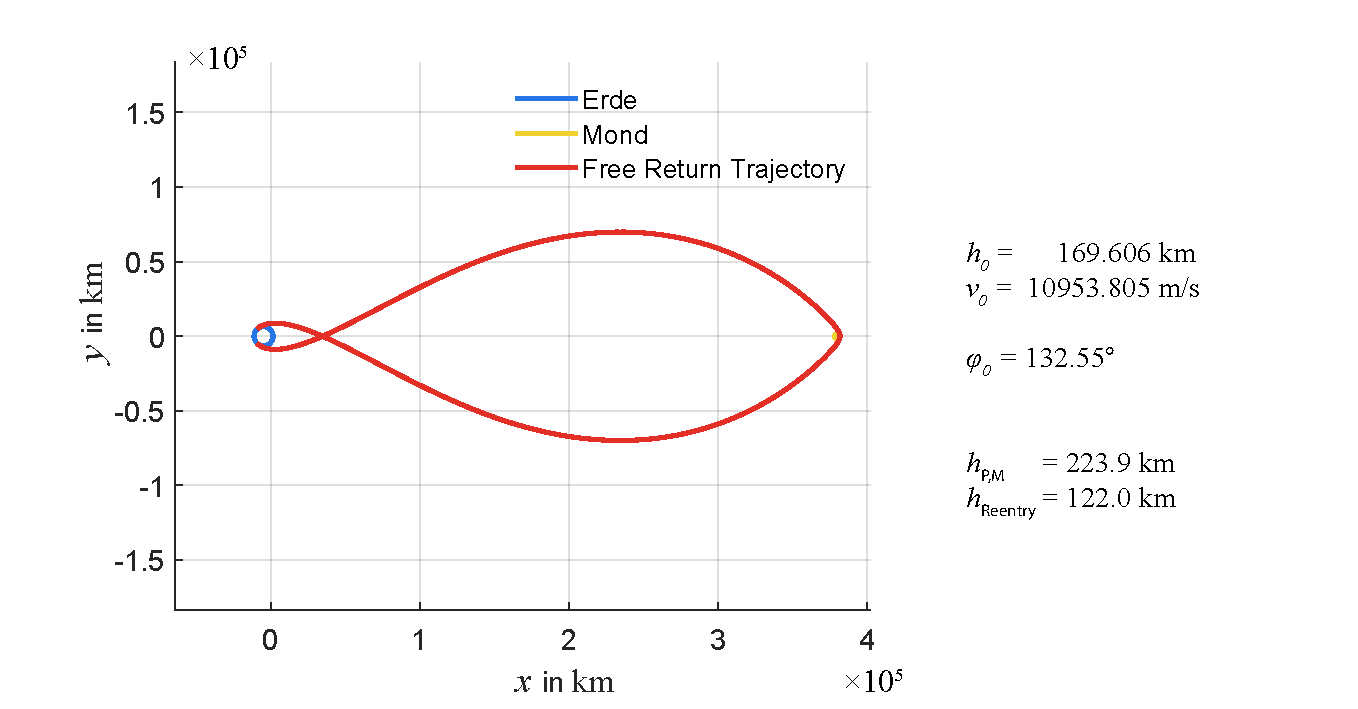
\includegraphics[width=\textwidth]{Transfer2MoonRotatingKOS.pdf} 
	\caption[Ergebnisse der numerischen Rechnung f�r das eingeschr�nkte Drei-K�rper-System Erde-Mond-Raumschiff.]{Ergebnisse der numerischen Rechnung f�r das eingeschr�nkte Drei-K�rper-System Erde-Mond-Raumschiff im mitrotierenden Koordinatensystem. Man beachte die unterschiedliche Form der Bahn, die wesentlich von der in \figref{adyn_FRT08} abweicht, was durch die unterschiedliche "`Perspektive"' des mitrotierenden Beobachters zustande kommt.}
	\label{abb:adyn_FRT10}
\end{figure}

Zum Schluss m�chten wir noch einmal bemerken, dass die FRT ein sch�nes Beispiel eines Swing-By-Man�vers (Gravity-Assist-Man�vers) (siehe \kap{adyn_gravity_assist}) beinhaltet und zwar ein Man�ver, bei welchem die Masse des Gravity-Assist-Himmelsk�rpers (in diesem Fall der Mond) abbremsend wirkt, da die Bahn nach \figref{adyn_swingby00} vor dem Himmelsk�rper liegt.

\end{subprobs}

\end{sol} 
\textcolor{blue} {$\rightarrow$ zur} \probref{adyn_rendezvous03}.\\
\noindent\rule[1ex]{\textwidth}{0.5pt}  \newpage  \clearpage

%-----------------------------------------------------------------------------------------------------------

\subsection{�bungen zu Starts aus der Erdatmosph�re und Wiedereintritt}

\noindent\rule[1ex]{\textwidth}{0.5pt} 

%-----------------------------------------------------------------------------------------------------------

\begin{sol}{prob:adyn_launch01a}\label{lsg:adyn_launch01a} %�bung25
\textbf{Bewegungsgleichungen f�r Raketenstart von Erdoberfl�che}\\

\begin{nebenrechnungNeu} {Nat�rliche Koordinaten}

(siehe \cite{Arens2008, Riley2006, Otto2019 })\\

Der zeitabh�ngige Einheitsvektor $\vec{t}$ der Tangente an die Bahnkurve (Tangentialvektor) ist definiert durch:
\begin{align}
    \vec{t} = \frac{\D \vec{r}}{\D s} ~~~\text{mit}~~~~\D s = | \D \vec{r}(t) | = \left| {\frac{\D \vec{r}}{\D t}} \right| \,  \D\,t= v(t)\; \D\,t\,,
\label{eq:adyn_NR_launch01}
\end{align}
worin $\D s$ die differentielle Bahnl�nge ist und $v$ der Betrag der Geschwindigkeit $\vec{v}$. Der Hauptnormalenvektor (ebenfalls eine Einheitsvektor) ist die 
normierte �nderung des Tangentialvektors �ber die Bahnl�nge:
\begin{align}
    \vec{n} = \frac{\D \vec{t}}{\D s} \big/ \left|\frac{\D \vec{t}}{\D s} \right|\,.
\label{eq:adyn_NR_launch02}
\end{align}
Aus $\vec{t}^2 =1 $ folgt $\D \vec{t} / \D s \cdot \vec{t} = 0$, \dh $\vec{n} \bot \vec{t}$, also $\vec{n} \cdot \vec{t} = 0$.
Damit kann man einen dritten Vektor definieren, der senkrecht auf dem Tangential- und dem Hauptnormalenvektor steht und Binormalvektor hei�t:
\begin{align}
    \vec{h} =  \vec{t} \times \vec{n}\,.
\label{eq:adyn_NR_launch03}
\end{align}
Die drei Vektoren $\vec{t},\,\vec{n},\, \vec{h}$ bilden ein (sogenanntes nat�rliches) Koordinatendreibein, das sich mit dem bewegten Objekt auf der Bahn mitbewegt und dabei sowohl einer Translation als auch Rotation unterliegt.
Die Geschwindigkeit $\vec{v}$ und die Beschleunigung $\vec{a}$ sind in diesen Koordianten dann definiert durch (\vgl Kap. 1.2.2. in Band I) 
\begin{align}
    \begin{split}
		    \vec{r} &=  v\,\vec{t}\\
        \vec{a} &=  \frac{\D}{\D t}\,\lk v\,\vec{t}\rk = \,\lek \dot{v}\,\vec{t} + v\,\dot{\vec{t}}\rek = \lek \dot{v}\,\vec{t} + v\,\vec{\omega}\times \vec{v}\rek\,.
    \end{split} \label{eq:adyn_NR_atmos03}
\end{align}
Hierin ist $\vec{\omega}$ die momentane Rotationsfrequenz des mitrotierenden \KOS definiert durch $\vec{t},\, \vec{n}$ und \vec{h}.\\

\end{nebenrechnungNeu}

Wir wollen zun�chst die momentane Rotationsfrequenz des nat�rlichen Dreibeins als Funktion von Bahnradius $r$ , Geschwindigkeit $v$ und FPA $\gamma$ berechnen. Wir betrachten dazu \figref{adyn_ueb_atmos01} und finden:
\begin{align}
    \vec{\omega} = \vec{\omega_1} + \vec{\omega_2} = (\omega_1 + \omega_2)\,\vec{h}\,,\label{eq:adyn_ueb_atmos05}
\end{align}
worin $\omega_1\,\vec{h}$ die Drehung durch die reine Bahnbewegung beschreibt und $\omega_2\,\vec{h}$ die Drehung des FPA ber�cksichtigt. Der Betrag von $\vec{\omega_1}$ ergibt sich aus \figref{adyn_ueb_atmos01} �ber $r\,\D\upsilon = |\D \vec{r}|\,\cos\gamma$ zu
\begin{align}
        \omega_1 = \dot{\upsilon} &= \frac{|\vec{v}|}{r}\,\cos\gamma = \frac{v}{r}\,\cos\gamma\, \label{eq:adyn_ueb_atmos05a} \,,
\end{align}
w�hrend der Betrag von $\vec{\omega_2}$ einfach der �nderungsrate des FPA entspricht (man beachte die Richtung!):
\begin{align}
        \omega_2 = - \dot{\gamma} \,.\label{eq:adyn_ueb_atmos05b}
\end{align}
Um die Bewegungsgleichung \eqref{eq:adyn_launch_vec},
\begin{align}
    m_\text{R}\lk t\rk \,\ddot{\vec{r}} = \vec{F}_\text{S}\lk t\rk + m_\text{R}\lk t\rk\,\vec{g}\lk \vec{r}\rk + \vec{F}_\text{D}\lk \vec{r},\dot{\vec{r}}\rk + \vec{F}_\text{A}\lk \vec{r},\dot{\vec{r}}\rk\, , \label{eq:adyn_ueb_atmos01}
\end{align}
in nat�rlichen Koordinaten schreiben zu k�nnen, schreiben wir die Kr�fte \bzw Beschleunigungen in \eqref{eq:adyn_ueb_atmos01} unter Ber�cksichtigung der Geometrie von \figref{adyn_launch02} in nat�rlichen Koordinaten (die Bewegung und alle Kr�fte sollen in einer Ebene liegen) und benutzen dabei den Angle of Attack $\alpha$ und den Flight Path Angle $\gamma$:
\begin{align}
\begin{split}
				\vec{F}_\text{S} &= F_\text{S}\,\cos\alpha\,\vec{t} + F_\text{S}\,\sin\alpha\,\vec{n}\,,~~~~\vec{F}_\text{A}  = F_\text{A}\,\vec{n}\,,~~~
        \vec{F}_\text{D} = -F_\text{D}\,\vec{t}\,,~~~\vec{g} = -g\,\sin\gamma\,\vec{t} -g\,\cos\gamma\,\vec{n}\,.
\end{split}\label{eq:adyn_ueb_atmos02}
\end{align} 
\begin{figure}[H]
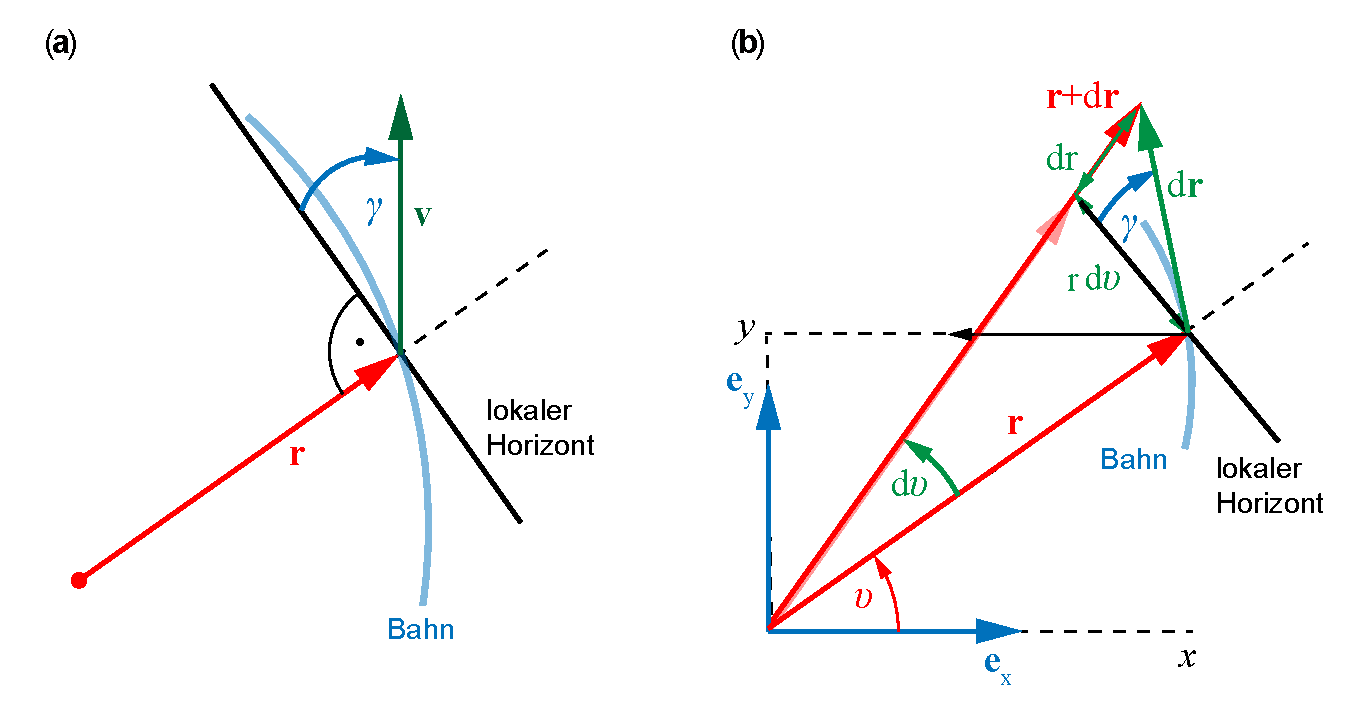
\includegraphics[width=\textwidth]{KOSReentry.pdf}
\caption[Zur Berechnung der Komponenten des Radialvektors einer Bahn im Inertialsystem der Erde.]{Zur Berechnung der Komponenten des Radialvektors einer Bahn im im Inertialsystem der Erde und im zylindrischen \KOS $\vec{t},\, \vec{n},\,\vec{h}$. \fa Lokaler Horizont, Geschwindigkeit und Flight Path Angle (FPA) $\gamma$. \fb Infinitesimale �nderungen von $r, \,\gamma$  und $v$. Der Winkel $\upsilon$ ist der Orbitalwinkel der Bahn (entspricht in etwa der wahren Anomalie) zwischen dem geozentrischen Ortsvektor zum Startpunkt und dem Ortsvektor zum Raumschiff zur Zeit $t$.}  

\label{abb:adyn_ueb_atmos01}
\end{figure}
Wir setzen \eqref{eq:adyn_ueb_atmos02} in \eqref{eq:adyn_ueb_atmos01} ein und erhalten eine Gleichung f�r $\vec{t}$ und $\vec{u}$.
\begin{align}
    \begin{split}
        \ddot{\vec{r}} &= \frac{\D}{\D t}\,\lk v\,\vec{t}\rk =  \lek \dot{v}\,\vec{t} + v\,\dot{\vec{t}}\rek = \lek \dot{v}\,\vec{t} + v \, \vec{\omega}\times \vec{v}\rek \\
        &= \lek \frac{F_\text{S}\,\cos\alpha - F_\text{D}} {m_\text{R}} \,- \,g\,\sin\gamma \rek\,\vec{t} + \lek \frac{F_\text{S}\,\sin\alpha + F_\text{A}}{m_\text{R}} - \,g\,\gamma\,\cos\gamma \rek\,\vec{n}\,.
    \end{split} \label{eq:adyn_ueb_atmos03}
\end{align}

Mit \eqref{eq:adyn_ueb_atmos05} - \eqref{eq:adyn_ueb_atmos05b} in \eqref{eq:adyn_ueb_atmos03} erhalten wir daraus jeweils eine Gleichung f�r $\vec{t}$ und 
$\vec{n}$, die jede f�r sich erf�llt sein muss, woraus folgt:
\begin{subequations}
    \begin{align}
        \dot{v}\,\vec{t} &= \lek \frac{F_\text{S}\,\cos\alpha-F_\text{D}}{m_\text{R}} - g\,\sin\gamma \rek\,\vec{t} \,, \\
        v\,\vec{\omega}\times \vec{v} &= \lk \dot{\theta}-\dot{\gamma}\rk\,\vec{h} \times v\,\vec{t}  = - \lek \frac{v^2}{r}\,\cos\gamma - v\, \dot{\gamma} \rek\,\vec{n} = \lek \frac{F_\text{S}\,\sin\alpha + F_\text{A}}{m_\text{R}} - \gamma\,g\,\cos\alpha \rek \,\vec{n}\,.
    \end{align} \label{eq:adyn_ueb_atmos04}
\end{subequations}

Nach einfacher Umformung erhalten wir schlie�lich die zwei verkoppelten skalaren Differentialgleichungen f�r $v$ und $\gamma$:
\begin{subequations}
    \begin{align}
        \dot{v} &= \frac{F_\text{S}\,\cos\alpha - F_\text{D}}{m_\text{R}} - g\,\sin\gamma\,,\\
        \dot{\gamma} &= \frac{F_\text{S}\,\sin\alpha + F_\text{A}}{v\,m_\text{R}} - \lk \frac{g}{v} -\frac{v}{r}\rk\,\cos\gamma\,~.
    \end{align}\label{eq:adyn_ueb_atmos06}
\end{subequations}

F�r den projizierten Kreisbogen $s(t)$, den das Raumschiff (eigentlich der Koordinatenursprung des mitbewegten \KOS) auf der Erdoberfl�che s(t) beschreibt, den Abstand des Raumschiffs vom Erdmittelpunkt  $r$ \bzw seine H�he $h$ �ber der Erdoberfl�che finden wir leicht aus geometrischen �berlegungen (\figref{adyn_launch02} und \figref{adyn_ueb_atmos01}):

\begin{subequations}
    \begin{align}
        \dot{h} &= v\,\sin\gamma\,,\\ 
        \dot{s} &= \frac{R_\text{E}}{r}\,v\,\cos\gamma \,=\, \frac{1}{1+h/R_\text{E}}\,v\,\cos\gamma  \,.
    \end{align}\label{eq:adyn_ueb_atmos07}
\end{subequations}

Das Differential-Gleichungssystem \eqref{eq:adyn_ueb_atmos06} und \eqref{eq:adyn_ueb_atmos07} bestimmt damit vollst�ndig die Aufstiegsbahn im mitbewegten KOS. Diese Bahn liegt in der durch die Richtungen von $s$ und $h = r - R_\text{E}$ bestimmten Ebene. 

\end{sol} 
\textcolor{blue} {$\rightarrow$ zur} \probref{adyn_launch01a}.\\
\noindent\rule[1ex]{\textwidth}{0.5pt}  \newpage  \clearpage
%-----------------------------------------------------------------------------------------------------------

\begin{sol}{prob:adyn_launch01}\label{lsg:adyn_launch01} %�bung26
\textbf{Raketenstart von verschiedenen Weltraumzentren}\\

\begin{subprobs}
\subprob{Allgemeine Betrachtungen}

\begin{figure}[H]
	\includegraphics[width=\textwidth]{Aufstiegsbahnen.pdf} 
	\caption[Transfer eines Raumschiffs von der Erdoberfl�che in einen Erdorbit �ber eine Hohmann-Ellipse.]{Transfer eines Raumschiffs von der Erdoberfl�che in einen Erdorbit �ber eine Hohmann-Ellipse. \fa idealisierter Fall ohne Reibung \fb realistischer Fall bei Vorhandensein einer Atmosph�re. Im idealisierten Fall w�rde man die Rakete horizontal direkt in die Hohmann-Ellipse starten lassen, im Fall \fb aus aerodynamischen und strukturellen senkrecht zum Horizont und f�hrt dann eine Nickkorrektur aus, um das Raumschiff einen \textit{Gravitation Turn}\index{Gravitation Turn}\index{Schwerkraftdrehung}  machen zu lassen. Siehe unten im Text.}
	\label{abb:adyn_launch_lsg_Schema}
\end{figure}

Wir k�nnen die Berechnungen vorteilhafter weise im in \kap{adyn_launch} eingef�hrten mitbewegten \KOS tun, da es uns nur um die Dynamik und nicht um eine geographische Berechnung der Bahn geht.\\
Zielstellung der Berechnung ist, das Raumschiff in eine Kreisbahn mit der H�he $h_\text{K}$ (numerische Werte beispielhaft f�r $h_\text{K}= \SI{300}{\km}$) zu bringen.\\
Ohne Atmosph�re w�rde man das Raumschiff horizontal in Richtung Osten von der Erde starten lassen (\figref{adyn_launch_lsg_Schema}a  und zwar mit einem Geschwindigkeitsbudget von
\begin{align}
	\Delta v_0 = \sqrt{\frac{G\,M_\text{E}}{R_\text{E}+h}} - \Delta v_\text{E,t} = \sqrt{\frac{G\,M_\text{E}}{R_\text{E}+h}} - \frac{2\pi\,R_\text{E}\,\cos\varphi_0}{\SI{86125}{\second}}\approx \SI{7.7309}{\km\per\second} - \SI{0.465}{\km\per\second}\,\cos\varphi_0 \,,
\end{align}
worin $\varphi_0$ die geographische Breite des Abschussortes ist und $\Delta v_\text{E,t}$ die Tangentialgeschwindigkeit auf der Erdoberfl�che der Erdrotation bezeichnet.
Das Raumschiff bewegt sich in diesem idealisierten Fall auf einer Hohmann-Ellipse (\kap{adyn_hohmann_transfer}) mit der Halbachse $a_\text{T}$ und der Exzentrizit�t $e_\text{T}$ (Numerische Werte f�r $h=\SI{300}{\km}$.)
\begin{align*}
	a_\text{T} &= \frac{1}{2} \, \lk R_\text{E} + h + R_\text{E} \rk = R_\text{E}+\frac{h}{2} \approx \SI{6528}{\km} \,,\\
  e_\text{T} &= \frac{h}{2R_\text{E}+h } \approx 0.022978\,.
\end{align*}
und br�uchte 
\begin{align}
	t_\text{f} = t_\text{T}= \pi\sqrt{\frac{a_\text{T}{}^3}{G\,M_\text{E}}} \approx \SI{43.5}{\minute}\,,
\end{align}
um in die Umlaufbahn zu gelangen, wo noch einmal entsprechend Gleichung \eqref{eq:adyn_hohmann04} ein Burn notwendig ist, um das Raumschiff aus der elliptischen Bahn in die Kreisbahn zu bringen.\\
In einem realistischen Fall (\figref{adyn_launch_lsg_Schema}b, \dh unter Ber�cksichtigung von Drag, wird das Raumschiff nach der Schubphase zum Zeitpunkt $t_\text{T}$ an einem �bergangspunkt T auf die Hohmann-Ellipse treffen. Dort m�ssen dann folgende Bedingungen erf�llt sein:\footnote{Hierbei haben wir die Gleichungen \eqref{eq:adyn_reentry02} benutzt. Wir hatten ja in \kap{adyn_reentry} darauf hingewiesen, dass diese Gleichungen sowohl f�r den De-Orbit als auch die Startphase gelten.}
\begin{subequations}
\begin{align}
    \cos\gamma_\text{T} &= \cos\gamma(t_\text{T})=\frac{1+e_\text{T}\,\cos\upsilon_\text{T}}{\sqrt{1+2e_\text{T}\,\cos\upsilon_\text{T} +e_\text{T}{}^2}}\,,\label{eq:adyn_launch_lsg01a}\\
    v_\text{T} &= v(t_\text{T}) = \sqrt{\frac{G\,M_\text{E}}{a_\text{T}(1-e_\text{T}{}^2}}\,\sqrt{1+2e_\text{T}\,\cos\upsilon_\text{T}+e_\text{T}{}^2} \label{eq:adyn_launch_lsg01b} \,,\\
    h_\text{T} &= r(t_\text{T}) - R_\text{E} = \frac{a_\text{T}\,\lk 1-e_\text{T}{}^2\rk}{1+e_\text{T}\,\cos\upsilon_\text{T}} - R_\text{E}\,.\label{eq:adyn_launch_lsg01c}
\end{align} \label{eq:adyn_launch_lsg01}
\end{subequations}

Hierin ist $\gamma_\text{T}$ der FPA und $\upsilon_\text{T}$ die wahre Anomalie der Hohmann-Ellipse zum Zeitpunkt $t_\text{T}$.\\
F�r den Startzeitpunkt $t=0$ gilt:
\begin{subequations}
\begin{align}
    \gamma_0 &= \gamma(t = 0)=  \pi/2 \label{eq:adyn_launch_lsg02a}\,,\\
    v_0 &= v(t=0) = 0 \label{eq:adyn_launch_lsg02b} \,,\\
    h_0 &= h(t=0) = 0 \,.\label{eq:adyn_launch_lsg02c}
\end{align} \label{eq:adyn_launch_lsg02}
\end{subequations}

Die Schubphase muss also durch geeignete Steuerung des Anstellwinkles (AoA) $\alpha(t)$, der Massenverlustrate $\dot(m)(t)$, des Schubs $F_\text{S}(t)$ und der Wahl von $\upsilon(t)$ so gestaltet werden, dass als Ergebnis der zeitlichen Entwicklung des DGL-Systems \eqref{eq:adyn_launch01} die Bedingungen \eqref{eq:adyn_launch_lsg01} erf�llt werden und dies bei m�glichst geringem Treibstoffverbrauch \bzw gro�er Nutzlast. Wir wissen nun aus \kap{adyn_launch}, Gleichung \eqref{eq:adyn_launch07}, dass ein AoA verschieden von Null zu Verlusten zus�tzlich zu den unvermeidlichen Gravitations- und Reibungsverlusten f�hrt. Andererseits zeigt die formale Integration von \eqref{eq:adyn_launch01} auch, dass ein $\alpha$ verschieden von Null zu einer gew�nschten Ver�nderung des FPA f�hrt.
\begin{subequations}
\begin{align}
    v(t_\text{T}) &= \int\limits_0^{t_\text{T}} \frac{F_\text{S}}{m_\text{R}}\,\D t' - \underbrace{\int\limits_0^{t_\text{T}} \frac{F_\text{D}}{m_\text{R}}  \,\D t'}_{\mathrm{Reibungsverlust}} - \underbrace{\int\limits_0^{t_\text{T}} \frac{F_\text{S}\,(1-\cos\alpha)}{m_\text{R}}  \,\D t'}_{\mathrm{Steuerungsverlust}}  - \underbrace{\int\limits_0^{t_\text{T}} g\,\sin\gamma \,\D t'}_{\mathrm{Gravitationsverlust}} \label{eq:adyn_launch_lsg03a} \,, \\
    \gamma(t_\text{T}) &= \frac{\pi}{2}+ \underbrace{\int\limits_0^{t_\text{T}} \frac{F_\text{S}\,\sin\alpha}{m_\text{R}\,v}  \,\D t'}_{\mathrm{Steuerungsverlust}} -  - \underbrace{\int\limits_0^{t_\text{T}}\frac{g}{v}\,\cos\gamma \,\D t'}_{\mathrm{Gravitationsverlust}} + \underbrace{\int\limits_0^{t_\text{T}}\frac{v}{r}\,\cos\gamma \,\D t'}_{\mathrm{Zentrifugalgewinn}} \nonumber \\
		&= \frac{\pi}{2} + \underbrace{\int\limits_0^{t_\text{T}} \frac{F_\text{S}\,\sin\alpha}{m_\text{R}\,v}  \,\D t'}_{\mathrm{Steuerungsverlust}} - \underbrace{\int\limits_0^{t_\text{T}} \lk \frac{g}{v} - \frac{v}{r} \rk \,\cos\gamma  \,\D t'}_{\mathrm{Gravitation~Turn}} \,. \label{eq:adyn_launch_lsg03b}
\end{align} \label{eq:adyn_launch_lsg03}
\end{subequations}

Das erscheint zun�chst wie ein Dilemma, denn erreicht man eine gro�e �nderung von $\gamma$, verliert man an Geschwindigkeit $v$. Zum Gl�ck gibt es, wie man am 2. Term in \eqref{eq:adyn_launch_lsg03b} sieht, den \textit{Gravitation Turn} (in etwa Schwerkraftdrehung), der sich aus der Kombination von Schwerkraft und Zentrifugalkraft\footnote{Da wir die Gleichungen \eqref{eq:adyn_launch01} im mitbewegten \KOS geschrieben haben tritt in diesen die Zentrifugalkraft auf.} f�r $\gamma \neq \pi/2$ ergibt und der automatisch Null wird, wenn $v$ gegen die Kreisbahngeschwindigkeit $\sqrt{g\,r}$ geht. Der Vorteil der Schwerkraftdrehung besteht darin, dass der Schub nicht dazu verwendet werden muss, um die Richtung des Raumfahrzeugs zu �ndern, und noch wichtiger, dass w�hrend der anf�nglichen Aufstiegsphase die Rakete eine Anstellwinkle von Null behalten kann, welcher die aerodynamischen Belastungen der Rakete erheblich reduziert.\\
Wie findet nun ein Raketenstart unter Nutzung der Schwerkraftdrehung statt?  Nach dem vertikalen Start gewinnt die Rakete zun�chst an Vertikalgeschwindigkeit und H�he. W�hrend dieses Teils des Starts wirkt der Schwerkraftwiderstand, der in der n�chsten Phase des Starts mit dem sogenannten Pitchover-Man�ver (Nick-Korrektur) reduziert wird.\footnote{Die Nick-Korrektur wird bei immer noch relativ geringen Vertikalgeschwindigkeiten durchgef�hrt, um aerodynamische Belastungen auf das Raumschiff zu vermeiden. Der Neigungswinkel des Pitchover-Man�ver betr�gt nur wenige Grad, es gibt aber auch F�lle, bei denn relativ gro�e Winkel (einige zehn Grad) verwendet werden. Die Nickkorrektur dauert \ia nur sehr kurz und ist der einzige Moment w�hrend der Aufstiegsphase, in dem der Schub zum Lenken genutzt wird. Nach dem Pitchover-Man�ver bleibt der AoA f�r den Rest des Aufstiegs bei Null, so dass auch der Auftrieb vernachl�ssigt werden kann.}
Das Pitchover-Man�ver dient zwei Zwecken. Erstens dreht es die Rakete leicht, so dass ihre Flugbahn nicht mehr vertikal verl�uft, und zweitens bringt es die Rakete auf den richtigen Kurs (Startazimut)\index{Startazimut} f�r ihren Aufstieg in die Umlaufbahn. Siehe dazu auch den folgenden L�sungsteil zum Startfenster (Launch Window) und  Startrichtung (Startazimut)). 

\subprob{Startphase einer dreistufigen Rakete (Ariane-1) im $\vec{t},\, \vec{n}$ und \vec{h} - \KOS.}

Im \mscr~\mladynref{Raketenstart2Orbit01.m} und \mladynref{Raketenstart2Orbit02.m} berechnen wir die f�r eine dreistufige Rakete den Transfer in den erdnahem Orbit.

\begin{figure}[H]
	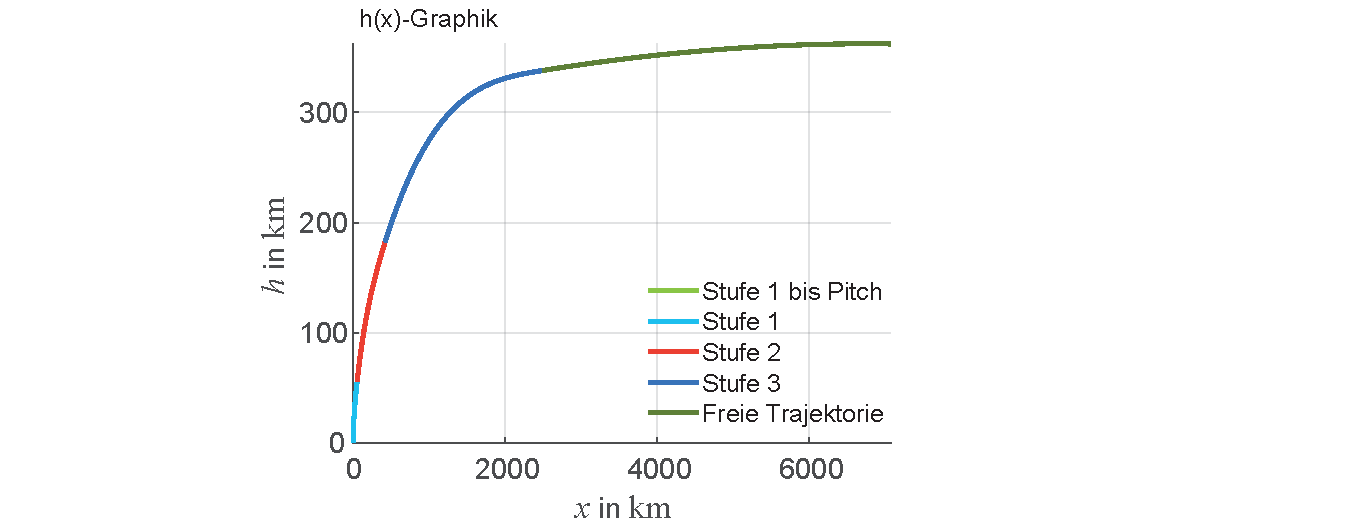
\includegraphics[width=\textwidth]{Startkurve.pdf} 
	\caption[Trajektorie nach Start von der Erdoberfl�che.]{Trajektorie nach Start von der Erdoberfl�che. Parameter siehe \mladynref{Raketenstart2Orbit02.m}.}
	\label{abb:adyn_launch_lsg02}
\end{figure}

\begin{figure}[H]
	\includegraphics[width=\textwidth]{Raketenstart2OrbitUebersicht.pdf} 
	\caption[Geschwindigkeit, Bahnh�he, FPA und Masse nach Start von der Erdoberfl�che. ]{Geschwindigkeit, Bahnh�he, FPA und Masse nach Start von der Erdoberfl�che f�r eine dreistufige Rakete bis zum �bergangspunkt (hier mit $h_\text{T} = \ca \SI{350}{\km}$ angenommen. Parameter siehe \mladynref{Raketenstart2Orbit02.m}.}
	\label{abb:adyn_launch_lsg03}
\end{figure}

\subprob{Startfenster (Launch Window) und  Startrichtung (Startazimut)}

Bisher haben wir uns nur mit der Dynamik und den energetischen Fragen eines Starts von der Erdoberfl�che und des anschlie�enden Transfer in eine gew�nschte Umlaufbahn besch�ftigt, nicht aber mit den Fragen nach der Zeit und den r�umlichen-geometrischen Bedingungen. Man k�nnte nat�rlich prinzipiell das Raumschiff zu jedem beliebigen Zeitpunkt starten und es auch an einen beliebigen Ort schie�en, um dann mit verschiedenen Bahnman�ver die Zielbahn zu erreichen. Aber das w�re eine enorme Verschwendung von Treibstoff. 

Unter einem Startfenster verstehen wir den Zeitraum, in welchem ein Raumschiff direkt in den gew�nschten Orbit \bzw auf eine geeignete Transferbahn (siehe vorhergehenden Abschnitt) gestartet werden kann. Dazu m�ssen wir abh�ngig vom gew�nschten Orbit und der geographischen Position des Abschussortes eine geeignet Startzeit und einen geeigneten Startwinkel finden. 

Hierbei gilt es zwei F�lle zu unterscheiden, zum einen, wenn die Inklination der gew�nschten Bahn $i$ gr��er oder gleich der geographischen Breite $\varphi_0$ des Startplatzes ist und zum anderen, wenn die Bahnneigung kleiner als die geographischen Breite ist. Wir werden sehen, dass es im zweiten Fall M�glichkeit gibt, direkt in den Orbit zu starten. 

Ein geeigneter Startzeitpunkt ist gegeben, wenn sich der Startort in der Position der Sternzeit des Startfensters (LWST) befinden, wobei  �in Position� hei�t, dass sich  Startplatz (bzw genauer der Breitenkreis des Startorts) und die gew�nschte Bahnebene schneiden. Wir betrachten dazu das sph�rische Dreieck in \figref{adyn_launch_lsg02}, welches durch drei Linien/Seiten gegeben ist. Die erste Seite ergibt sich aus der Bodenspur f�r die Umlaufbahn, die zweite aus der �quatorlinie und die dritte aus dem L�ngenkreis des Startplatzes. 
Aus \figref{adyn_launch_lsg02} entnehmen wir ferner noch weitere Gr��en mit folgenden Definitionen und Beziehungen:\\

\begin{tabular}[h]{ll}
LWST &~Sternzeit des Startfenster\index{Startfenster} (Launch Window Siderial Time)\index{Launch Window Siderial Time}\\
$\delta$ &~Hilfswinkel in Startrichtung\\
$\theta$ &~Standortwinkel des Startfensters\\
$\beta$  &~Startazimut\index{Startazimut}\\
$\Omega$ &~Rektaszension des aufsteigenden Knotens\\
\end{tabular}

\begin{figure}[H]
	\includegraphics[width=\textwidth]{BestimmungLWST.pdf} 
	\caption[LST und sph�risches Dreieck zur Bestimmung des LWST.]{LST \fa und sph�risches Dreieck zur Bestimmung des LWST \fb.}
	\label{abb:adyn_launch_lsg04}
\end{figure}

Mit dem Winkelkosinussatz der sph�rischen Trigonometrie \cite{Meyers1995} $~\cos \alpha = -\cos\beta\,\cos\gamma\,+\,\sin\beta\,\sin\gamma\,\cos a$ 
finden wir 
\begin{align*}
\cos i = -\cos(\pi/2)\,\cos\delta\,+\,\sin(\pi/2)\,\sin\delta\,\cos \varphi_0\,,
\end{align*}
was sich mit $\cos(\pi/2) = 0$ und $\sin(\pi/2) = 1$ zu
\begin{align}
\sin \delta = \cos i / \cos \varphi_0\, \label{eq:adyn_launch_lsg04}
\end{align}
vereinfacht. F�r das rechtwinklige sph�rische Dreieck gilt au�erdem \cite{Meyers1995}: $\cos \delta = \cos \theta \,\sin i~$, 
woraus schlie�lich mit \eqref{eq:adyn_launch_lsg03}
\begin{align}
\cos \theta = \frac{\cos \delta }{\sin i} = \frac{\sqrt{1 - \sin^2\delta}}{\sin i} = \frac{\sqrt{\lk 1 - \cos^2 i / \cos^2 \varphi_0 \rk}}{\sin i}
\label{eq:adyn_launch_lsg05}
\end{align}
folgt. F�r die n�rdliche Hemisph�re ergibt sich damit das LWST zu:
\begin{align}
\text{In der N�he des aufsteigenden Knotens: ~~~}\mathrm{LWST}_\text{auf} &= \Omega + \theta ~\,, \label{eq:adyn_launch_lsg06} \\
\text{In der N�he des absteigenden Knotens: ~~~~}\mathrm{LWST}_\text{abs} &= \Omega + (180\degree - \theta) \,. \label{eq:adyn_launch_lsg07}
\end{align}

\begin{figure}[H]
	\includegraphics[width=\textwidth]{StartAzimute.pdf} 
	\caption[Startazimut.]{Startazimut in der N�he des \fa aufsteigenden Knotens und des \fb absteigenden Knotens.}
	\label{abb:adyn_launch_lsg05}
\end{figure}

Es gibt noch einen letzten Winkel, der ber�cksichtigt werden muss, n�mlich das Startazimut $\beta$, \dh die Richtung in die gestartet werden soll. Dies ist der Winkel zwischen dieser �Aufw�rts�-Richtung und der Startrichtung (\figref{adyn_launch_lsg03}) und wird von der Nordrichtung aus im Uhrzeigersinn gemessen. Er ist vom Betrag her gleich dem Winkel $\delta$, womit wir schreiben k�nnen:
\begin{align}
\beta = \arcsin \frac{\cos i}{\cos \varphi_0}\,. \label{eq:adyn_launch_lsg08}
\end{align}
Wir erkennen an dieser Beziehung auch, dass die erreichbare Neigung der Bahn immer gr��er als die geographische Breite des Startortes sein muss, andernfalls w�rde $\beta$ komplexe Werte annehmen. Es gilt also immer $i \geq \varphi_0$, wobei die minimal Bahnneigung bei einem Startazimut von $90\degree$ (entspricht Ost) erreicht wird (\figref{adyn_launch_lsg04}).\\
F�r ein gegebenes $\Omega$ der Bahn gibt es  zwei L�sungen oder Startzeiten pro Rotation. Bei jeder davon kann man dann zwischen prograden und retrograden Umlaufbahnen w�hlen. Diese werden entlang der berechneten Startazimute in Richtung Norden oder S�den verlaufen, wobei die Startfenster einige Zeit auseinander liegen. Es gibt nur eine L�sung, wenn die Neigung genau dem Breitengrad entspricht.  Wir wolle zwei Beispiele angeben (siehe auch \mscr~\mladynref{Raketenstart2Orbit03.m}).

\begin{figure}[H]
	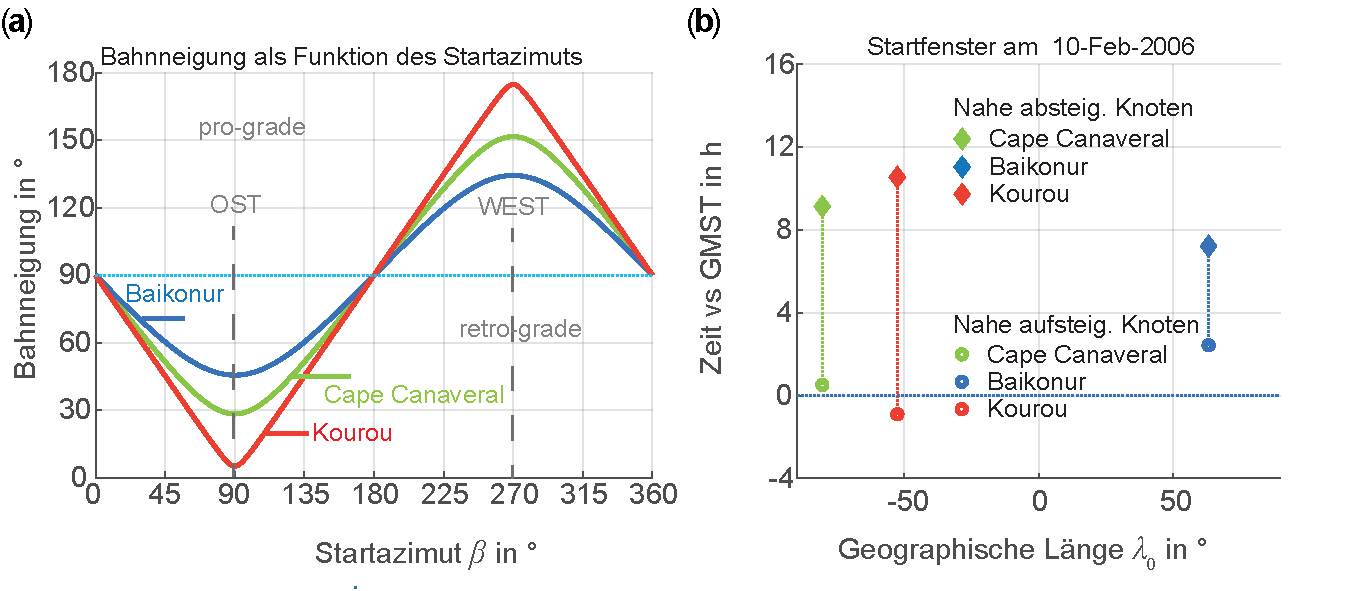
\includegraphics[width=\textwidth]{StartAzimuteStartFenster.pdf} 
	\caption[Bahnneigung und Startfenster als Funktion des Startazimuts und Startfenster zur ISS.]{Bahnneigung \fa und Startfenster \fb als Funktion des Startazimuts f�r verschiedene Weltraumzentren.}
	\label{abb:adyn_launch_lsg06}
\end{figure}

Die Internationale Raumstation umkreist die Erde mit einer Neigung von $51.6\degree$. F�r einen Start von Cape Canaveral (Breitengrad $28.383\degree$) \bzw vom Kosmodrom Baikonur (Breitengrad 45.617�) in die ISS-Umlaufbahn berechnen sich die Startazimute zu:
ergibt sich dann:
\begin{align*}
\beta_\text{CC}  &= \arcsin \frac{\cos(51.6\degree)}{\cos(28.383\degree)} = 44.98\degree~~ \text{\bzw}~~135.02\degree\,,\\ 
\beta_\text{Bai} &= \arcsin \frac{\cos(51.6\degree)}{\cos(45.617\degree)} = 63.21\degree~~ \text{\bzw}~~116.80\degree\,. 
\end{align*}

Die Berechnung der  Startfenster und Startazimute f�r die ISS f�r den 10. M�rz 2006 ist im \mscr~\mladynref{Raketenstart2Orbit03.m}\, ausgef�hrt.
F�r die ISS haben wir daf�r folgende Bahnparameter f�r Anfang 2006 benutzt \cite{JPL2020}.\\

\begin{tabular}{L{7cm}C{2cm}L{4cm}}
Epoche & $t_\text{epoch}$ & 09.02.2006 20:26:00.0000\\
Inklination &$i$ & $51.6448\degree$\\
Rektaszension des aufsteigenden Knotens & $\Omega$ & $122.3522\degree$\\
numerische Exzentrizit�t der Umlaufbahn & $e$ & 0.0008835\\
Argument des Perig�ums & $\omega$ &$257.3473\degree$\\
Mittlere Anomalie & $M$ & $251.7436\degree$\\
Mittlere Bewegung & $n$ & $ \SI{15.74622749}{\per\day}$\\
\end{tabular}
\medskip

Die Sternzeit in Greenwich bestimmt man aus dem Julianischen Datum JD f�r den Zeitpunkt 0:00 h UTC. Zun�chst berechnet man das Julianische Datum in Jahrhunderten seit dem 1.1.2000. 
	\[ T\,=\,\frac {JD-2451545.0}{36525} \]
und daraus die mittlere Sternzeit f�r Greenwich f�r den Zeitpunkt 0:00 h UTC:
\begin{align}
\mathrm {GMST_0} \,&=\,6^{\mathrm {h} }41^{\mathrm {m} }50.54841^{\mathrm {s}}\,+\,8640184.812866^{\mathrm {s} }\, T\,+\,0.093104^{\mathrm {s} }\, T^{2}\,-\,0.0000062^{\mathrm {s} }\, T^{3}\\
&=\,24110.54841^{\mathrm {s} }+8640184.812866^{\mathrm {s} }\, T \, + \,0.093104^{\mathrm {s} }\, T^{2}\,-\,0.0000062^{\mathrm {s} }\, T^{3}\\
&=\,100.46061837\degree+36000.770053608\degree\, T\,+\,0.000387933\degree\, T^{2}\,-\,(T^{3}/38710000)\degree
\end{align}
F�r einen Beobachter auf der geographischen L�nge $\lambda_0$ muss man die Sternzeit noch auf seine Ortssternzeit LST umrechnen:
\begin{align}
\mathrm {LST} \,&\,=\mathrm {GMST} +\lambda~~~{\text{f�r GMST im Gradma�}}
\end{align}

Wir verweisen auf das \mscr~\mladynref{Raketenstart2Orbit03.m} und auch auf \kap{hm_zeitdefinition}.


\subprob{Berechnung der 3D-Trajektorien im Inertialsystem}


F�r die weiteren Berechnungen muss man ber�cksichtigen, das wir alle Gr��en wie \zb das in \eqref{eq:adyn_launch_lsg08} abgeleitete Startazimut im Inertialsystem berechnet hatten. Da wir jedoch die Rakete von der rotierenden Erdoberfl�che starten, muss man die Erddrehung entsprechend ber�cksichtigen, was zu einer leichten Korrektur des Startazimuts und auch des Geschwindigkeitsbudgets f�hrt. Wir wollen ab sofort zur besseren Unterscheidung die Gr��en im mitbewegten System gestrichen kennzeichnen, die im Inertialsystem als ungestrichen.
So ist \zb f�r eine Umlaufbahn von 300 km H�he das Mindestgeschwindigkeitsbudget $\Delta \vec{v}$ (ohne Reibung und Reserven) durch $\Delta \vec{v} = \Delta v\,(\sin \beta\,\veceX + \cos \beta\,\veceY)$ mit $\Delta v = \SI{7.7309}{\km\per\second}$ gegeben, wobei die Einheitsvektoren in der Bahnebene liegen und in die Ost- \bzw Nordrichtung zeigen. Am einfachsten macht man sich nun an Hand von \figref{adyn_launch_lsg07} klar, dass zur Berechnung des Geschwindigkeitsbudget $\Delta \vec{v}'$ im Nichtinertialsystem die vektorielle Differenz von $\Delta \vec{v}$ und $\Delta v_\text{E,t}\,\veceX = \SI{0.465}{\km\per\second}\,\cos\phi_0$ (\vgl \eqref{eq:adyn_launch10}) gebildet werden muss. Man erh�lt:
\begin{align}
\Delta v' = \Delta v \, \sqrt{\lk \sin \beta \, - \Delta v_\text{E,t}/ \Delta v \rk^2 + \cos^2 \beta}\,. \label{eq:adyn_launch_lsg09}
\end{align}
Das Startazimut im mitbewegten System $\beta'$ ergibt sich dann zu:
\begin{align}
\beta' = \arctan \lk \frac{\Delta v\,\sin \beta\, - v_\text{E,t}}{\Delta v\,\cos \beta\,} \rk\,. \label{eq:adyn_launch_lsg10}
\end{align}
F�r einen Start zur ISSS von Cape Canaveral �ndert es sich beispielsweise von $44.98\degree$ auf $42.76\degree$. Auch der FPA rechnet sich enstprechend um zu:
\begin{align}
\gamma = \arcsin \lk \frac{\Delta v'}{\Delta v}\,\sin \gamma' \rk\,. \label{eq:adyn_launch_lsg11}
\end{align}

\begin{figure}[H]
	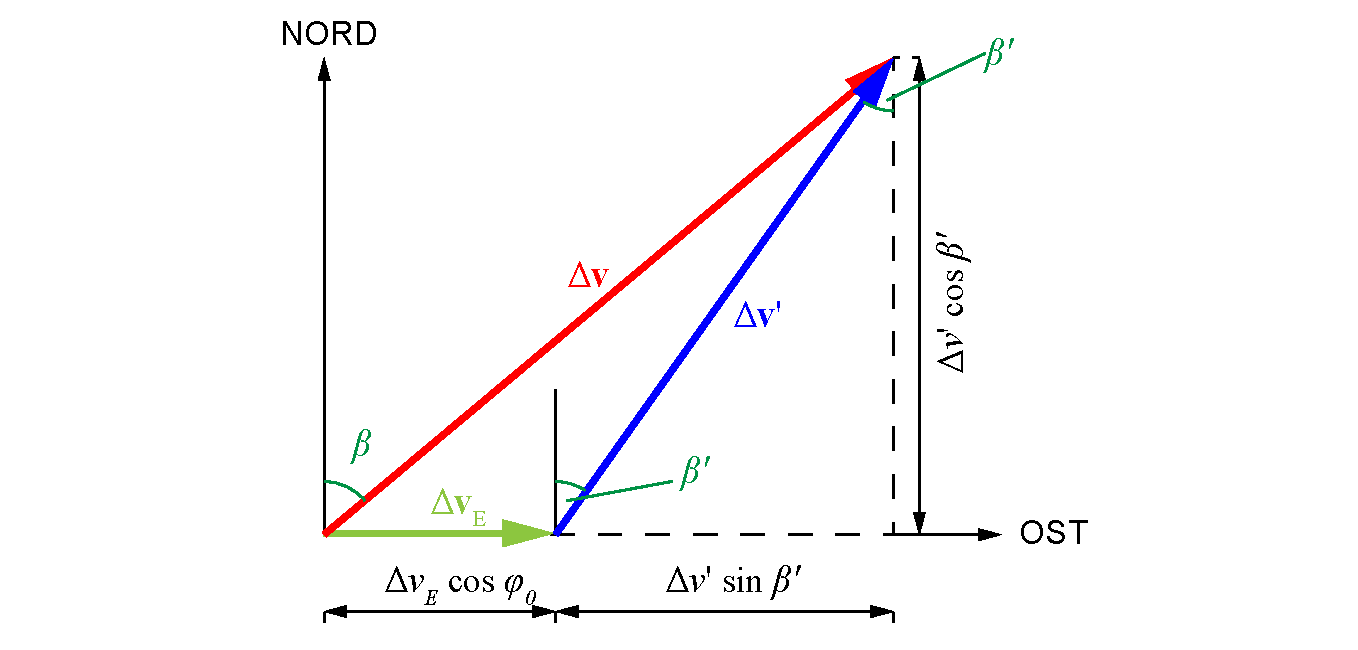
\includegraphics[width=\textwidth]{StartAzimutInertial.pdf} 
	\caption[Ber�cksichtigung der Erdrotation beim Start von Raketen.]{Ber�cksichtigung der Erdrotation beim Start von Raketen.}
	\label{abb:adyn_launch_lsg07}
\end{figure}

F�r die Berechnung der 3D-Trajektorien haben wir drei M�glichkeiten:
\begin{enumerate}[a)]
	\item Wir betrachten alles im geozentrisch-raumfesten Inertialsystem und l�sen numerisch die Bewegungsgleichung \eqref{eq:adyn_launch_vec} in 3 Dimensionen. Dabei m�ssen wir bei den Anfangsbedingungen die von der Rakete mitgenommene Rotation der Erde nach \eqref{eq:adyn_launch_lsg09} ber�cksichtigen, ebenso wie das umgerechnete Startazimut $\beta$ und den Anfangs-FPA $\gamma_0$ nach \eqref{eq:adyn_launch_lsg10} \bzw \eqref{eq:adyn_launch_lsg11}. Man beachte, dass die beiden Gr��en im topozentrischen System definiert sind und mit den Ortskoordinaten des Startorts in das Inertialsystem umgerechnet werden m�ssen.\\
	Bei der Berechnung der Reibung muss man ber�cksichtigen, dass die Atmosph�re mitrotiert und folglich die f�r die Reibung ma�gebliche aktuelle Geschwindigkeit $v'$ aus der im Inertialsystem geltenden Geschwindigkeit in $v$ umgerechnet werden muss:
\begin{align}
\begin{split}
		\vec{v}'(t) &= \vec{v}(t) - \vec{v}_\text{E,0} ~~~\text{mit}~~~\vec{v}_\text{E,0} = \vec\omega_\text{E} \times \vec{r}_0 \,.
\end{split} \label{eq:adyn_launch_lsg12}
\end{align}
Die Bewegungsgleichung lautet also:
\begin{align}
\begin{split}
		\vec{\ddot{r}}\begin{pmatrix} \ddot{x}\\ \ddot{y} \\ \ddot{z} \end{pmatrix} &=  \frac{\vec{F}_\text{S}(t) + \vec{F}_\text{G}(t) - \vec{F}_\text{D}(t)}{m_\text{R}(t)} = 
		\frac{F_\text{S}(t)}{m_\text{R}(t)\,v(t)} \begin{pmatrix} \dot{x}\\ \dot{y} \\ \dot{z} \end{pmatrix} 
 - \frac{G\,M_\text{E}}{\left| \vec{r}(t) \right|^3} \begin{pmatrix} x \\y\\z \end{pmatrix}
 - \frac{\varrho(r)\, v'\, A \,c_\text{D}}{m_\text{R}(t)} \begin{pmatrix} \dot{x}'\\ \dot{y}'\\ \dot{z}' \end{pmatrix}\,.
\end{split} \label{eq:adyn_launch_lsg13}
\end{align}
Die Nickkorrektur wird wie folgt berechnet:\\ 
Nach Bestimmung der Geschwindigkeit zum Zeitpunkt kurz vor der Nickkorrektur $\vec{v}(t=t_\text{Nick-})$, die sich ohne der mitgenommenen
Rotation der Erde ergibt (also nur die Geschwindigkeitszunahme durch den Schub), erfolgt 
die Drehung des Geschwindigkeitsvektors/Schubvektors um den Nickwinkel $\gamma_\text{N}$ in Richtung des Startazimuts. Diese Drehung wird im Horizontsystem 
mit folgender Drehmatrix $\mathbb{R}_\text{Nkorr}$ beschrieben, wobei hierbei zuerst die
Nickkorrektur und dann die Ausrichtung auf das Azimut ausgef�hrt wird. Die dazu notwendigen Berechnung der Drehmatritzen f�hren wir in einer Nebenrechnung aus:

\begin{nebenrechnungNeu} {Einheitsvektoren und Transformationsmatrix}

\begin{align*}
    \vec{r} &= r\,\begin{pmatrix} \sin\theta\,\cos\phi \\ \sin\theta\,\sin\phi \\ \cos\phi \end{pmatrix} ~~ \text{\bzw in geograph. Koord.}~~~ \vec{r} = r\,\begin{pmatrix} \cos\varphi\,\cos\lambda \\ \cos\varphi\,\sin\lambda \\ \sin\varphi \end{pmatrix}\\
    \vec{e}_\text{r} &= \frac{\d\vec{r}}{\d r} \;= \;\begin{pmatrix} \sin\theta \,\cos\phi \\ \sin\theta\,\sin\phi \\ \sin\phi \end{pmatrix}\; \widehat{=} \;\begin{pmatrix} \cos\varphi\,\cos\lambda \\ \cos\varphi\,\sin\lambda \\ \sin\varphi \end{pmatrix}\\
     \vec{e}_\theta &= \frac{1}{r}\,\frac{\d\vec{r}}{\d \theta}\;=\; \begin{pmatrix} \cos\theta \,\cos\phi \\ \cos\theta \,\sin\phi \\ -\sin\phi \end{pmatrix}\;\widehat{=}\;\vec{e}_\varphi = \frac{1}{r}\,\frac{\d\vec{r}}{\d \varphi}\;=\; \begin{pmatrix} -\sin\varphi \,\cos\lambda \\ -\sin\varphi\,\sin\lambda \\ \cos\varphi \end{pmatrix} \\
     \vec{e}_\phi &= \frac{1}{r\,\sin\theta}\,\frac{\d\vec{r}}{\d \phi}\;=\; \begin{pmatrix} -\sin\phi\\ \cos\phi \\ 0 \end{pmatrix}\;\widehat{=}\;\vec{e}_\lambda = \frac{1}{r\,\cos\varphi}\,\frac{\d\vec{r}}{\d \lambda}\;=\; \begin{pmatrix} -\sin\lambda \\ \cos\lambda\\ 0 \end{pmatrix} \\
    \rightarrow \mathbb{S} &= \lk \vec{e}_\text{r},\,\vec{e}_\theta,\,\vec{e}_\phi \rk \;=\; \begin{pmatrix} \cos\varphi\,\cos\lambda & -\sin\phi\,\cos\varphi & -\sin\lambda \\ \cos\varphi\,\sin\lambda & -\sin\varphi\,\cos\lambda & \cos\lambda \\ \sin\varphi & \cos\varphi& 0 \end{pmatrix}
\end{align*}

\end{nebenrechnungNeu}

Wir erhalten damit:

\begin{align}
\begin{split}
		\mathbb{R}_\text{Nkorr} &= \mathbb{R}_\text{A}\, \mathbb{R}_\text{N} ~~\text{mit}~~\\
		\mathbb{R}_\text{N} &= \begin{pmatrix} \cos\gamma_\text{N} & ~~-\sin\gamma_\text{N} & ~~0 \\
		                                      \sin\gamma_\text{N} & ~~+\cos\gamma_\text{N} & ~~0 \\
																					0 & 0 & 1\end{pmatrix}\ ~~\text{und}~~
		\mathbb{R}_\text{A} = \begin{pmatrix} 1 &~~ 0 &~~ 0 \\
		                                      0 &~~\cos\beta' & ~~-\sin\beta'\\
		                                      0 &~~\sin\beta' & ~~+\cos\beta' \end{pmatrix}\,.
\end{split} \label{eq:adyn_launch_lsg14}
\end{align}
Die so berechnete Drehmatrix geht jedoch davon aus, dass die Rakete vor der
Nickkorrektur entlang der $x$-Richtung der Drehmatrix ausgerichtet ist. In unserem Fall ist die Rakete aber radial nach au�en gerichtet. Daher muss die Drehmatrix noch
in das richtige (sph�rische) Koordinatensystem transformiert werden. (Siehe auch \mscr~\mladynref{KOS.m}):
\begin{align}
\begin{split}
  \mathbb{R}_\text{Nkorr}' &= \mathbb{S} \,\mathbb{R}_\text{Nkorr}\, \mathbb{S}^\text{T}~~~\text{mit}~~~\\
	\mathbb{S} &= \begin{pmatrix} \vec{e}_r  & \vec{e}_\varphi &\vec{e}_\lambda \end{pmatrix} =
	              \begin{pmatrix} \cos\varphi\,\cos\lambda &~~ -\sin\varphi\,\cos\lambda &~~ -\sin\lambda\\
			                          \cos\varphi\,\sin\lambda &~~ -\sin\varphi\,\sin\lambda &~~ +\cos\lambda\\
			                          \sin\varphi)                &~~ +\cos\varphi                &~~ 0 \end{pmatrix}\,.
\end{split} \label{eq:adyn_launch_lsg15}
\end{align}
Der Geschwindigkeitsvektor (zugleich die Schubrichtung) der Rakete nach Nickkorrektur ist dann:
\begin{align*}
\vec{v}(t=t_\text{Nick+})  = \mathbb{R}_\text{Nkorr}'\,\vec{v}(t=t_\text{Nick-})\,.
\end{align*}
Wir bestimmen die H�he, den FPA, die Geschwindigkeit und die Masse der Rakete f�r die einzelnen Stufen bis die Rakete einen FPA von 0 hat. Dann erfolgt nur noch ein tangentialer Schub bis zum Erreichen der notwendigen Kreisbahngeschwindigkeit. 

Das Ergebnis der Rechnungen ist in \figref{adyn_launch_lsg08} und \figref{adyn_launch_lsg09} dargestellt und im \mscr~\mladynref{Raketenstart2Orbit04.m} ausgef�hrt und ausf�hrlich erl�utert.

\begin{figure}[H]
	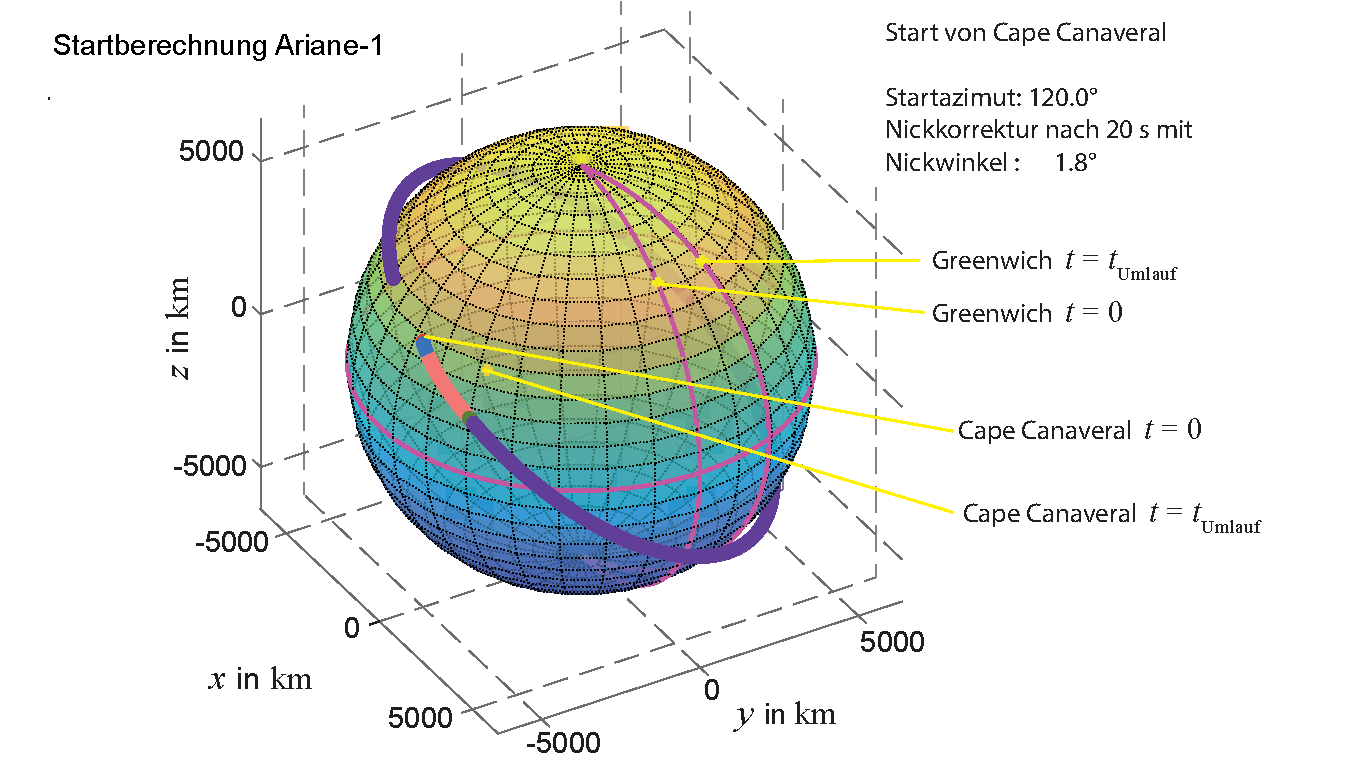
\includegraphics[width=\textwidth]{StartAriane01.pdf} 
	\caption[Trajektorie nach Start von der Erdoberfl�che.]{Trajektorie nach Start von der Erdoberfl�che. Parameter siehe \mladynref{Raketenstart2Orbit04.m}.}
	\label{abb:adyn_launch_lsg08}
\end{figure}

\begin{figure}[H]
	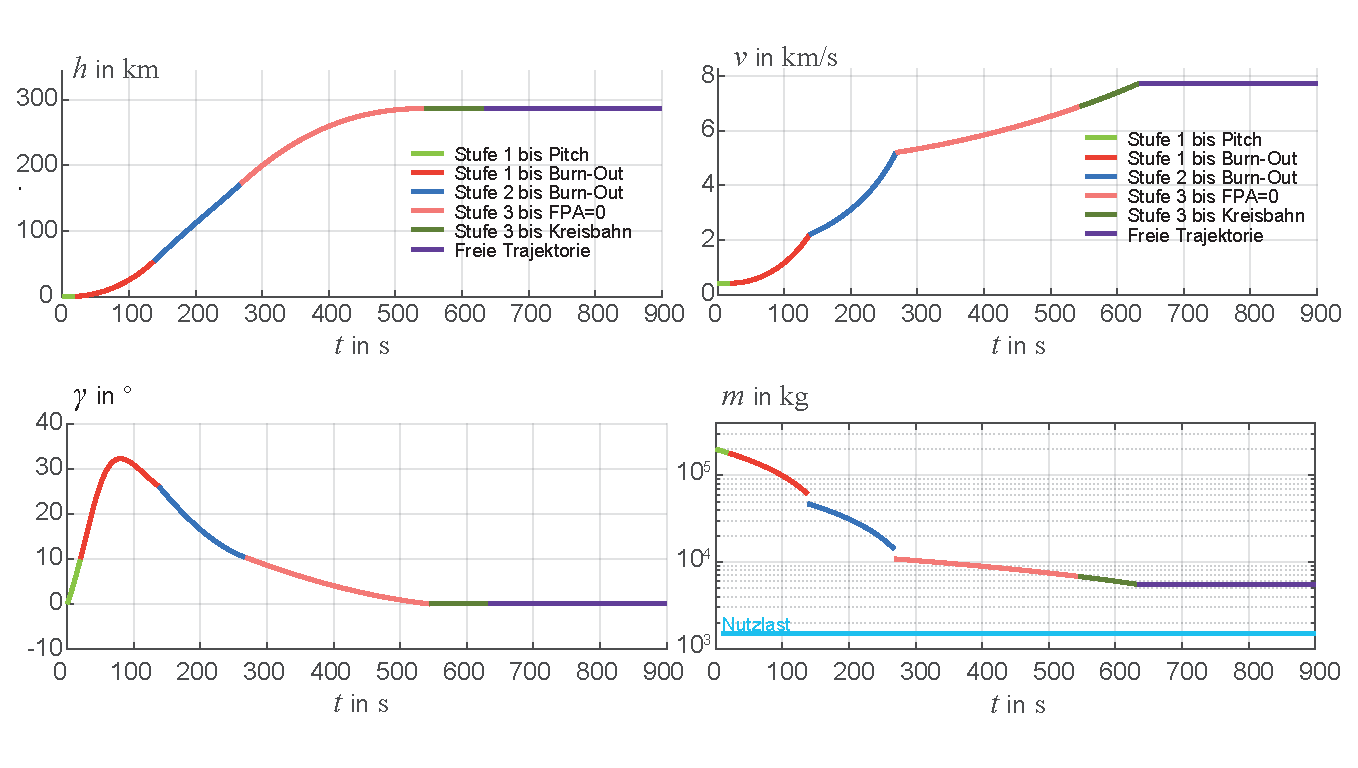
\includegraphics[width=\textwidth]{StartAriane02.pdf} 
	\caption[H�he, FPA,  Geschwindigkeit und  Masse der Ariane 1 nach Start von der Erdoberfl�che.]{H�he, FPA,  Geschwindigkeit und  Masse der Ariane 1 nach Start von der Erdoberfl�che. Parameter siehe \mladynref{Raketenstart2Orbit04.m}.}
	\label{abb:adyn_launch_lsg09}
\end{figure}

\item Als Alternative kann man die Trajektorien nat�rlich auch im mitbewegten \KOS des Beobachters im Horizontsystem berechnen. Das f�hrt auf �hnliche Rechnungen wie wir im Kap. 1.3.2 im Band I (Physik Bewegung) zum Wurf und freien Fall auf der Erdoberfl�che gemacht hatten.
\item Als weitere Alternative k�nnen wir nat�rlich das Ergebnis der Rechnungen im mitbewegten \KOS (Siehe Teilaufgabe 2) benutzen und ins Inertialsystem transformieren. Zwei Ortsvektoren sind dabei ausgezeichnet: Der Vektor zum Startpunkt und der Vektor zum aufsteigenden Knoten. Die Inklination und der aufsteigende Knoten der Bahn sind durch Startazimut, Startfenster und geographische Position des Startortes gegeben. Die Transformation erfolgt �ber die im \kap{hm_bahnen_hk_PQR} hergeleiteten Matrizen.\\
Wir empfehlen dem Leser zur Vervollst�ndigung des Bildes beide Alternativen selbst zu rechnen.
\end{enumerate}

\end{subprobs}
\end{sol} 
\textcolor{blue} {$\rightarrow$ zur} \probref{adyn_launch01}.\\
\noindent\rule[1ex]{\textwidth}{0.5pt}  \newpage  \clearpage

%-----------------------------------------------------------------------------------------------------------

\begin{sol}{prob:adyn_reentry01}\label{lsg:adyn_reentry01} %�bung27
\textbf{Parameter des Wiedereintritts in die Erdatmosph�re}\\

\begin{figure}[H]
\includegraphics[width=\textwidth]{ReentryGeometrie01.pdf}
\caption[Geometrie des Wiedereintritts in die Erdatmosph�re.]{Geometrie des Wiedereintritts in die Erdatmosph�re. Siehe auch \mscr~\mladynref{Transfer2Reentry.m} f�r weitere Details und Graphiken.}
\label{abb:adyn_reentry_geometrie01}
\end{figure}

\begin{figure}[H]
\includegraphics[width=\textwidth]{ReentryGeometrie02.pdf}
\caption[Geometrie des Wiedereintritts in die Erdatmosph�re.]{Geometrie  (Detail) des Wiedereintritts in die Erdatmosph�re. Siehe auch \mscr~\mladynref{Transfer2Reentry.m} f�r weitere Details und Graphiken.}
\label{abb:adyn_reentry_geometrie02}
\end{figure}

%\begin{nebenrechnung}
%\begin{align*}
    %e &= \frac{q^2-\lk 2q-1\rk\,\cos^2\gamma_\text{Re}}{q^2-\cos^2\gamma_\text{Re}} = \frac{q^2-\lk 2q-1\rk\,u^2}{q^2-u^2} \\
    %\cos\theta_\text{Re} &= q\,\frac{\lk 1-e\rk}{e}-\frac{1}{e} = \frac{q-1}{e}-q = \frac{Z}{N}\\
    %&= \frac{\lk q-1\rk\lk q^2-u^2\rk-q\,\lk q^2-\lk 2q-1\rk\,u^2\rk}{q^2-\lk2q-1\rk\,u^2}\\
    %N &= q^2-2\,q\,u^2+ u^2 = q^2-2q+1+2q-1-2\,q\,u^2+u^2\\
    %&= \lk q-1\rk^2 +\lk 2q-1\rk - \lk 2q-1\rk\,u^2 \\
    %&= \lk q-1\rk^2 + \lk2q-1\rk\lk1-u^2\rk \\
    %&= \hat{q}^2 + \lk 2q-1\rk\,\sin^2\gamma_\text{Re}\\
    %Z &=  \cancel{q^3} - \cancel{q\,u^2}-q^2+u^-\cancel{q^3} +2\,q^2\,u^2-\cancel{q\,u^2} = 2\,q^2\,u^2- 2\,q\,u^2 - q^2+u^2 \\
    %&= \lk q^2-2q+1\rk\,u^2 - \lk q^2-q^2\,u^2\rk = \hat{q}^2\,u^-q^2\,\lk1-u^2\rk\\
    %&= \hat{q}^2\,\cos^2\gamma_\text{Re} - q^2\,\sin^2\gamma_\text{Re}
%\end{align*}
%\end{nebenrechnung}

Wir haben die Geometrie des Deorbits in \figref{adyn_reentry_geometrie01} und \figref{adyn_reentry_geometrie02} dargestellt.\\
Gegeben sind $v_\text{A}$, $r_\text{A}$, $r_\text{Re}$ und der gew�nschte FPA $\gamma_\text{Re}$, gesucht sind der \anf{Ort} $\upsilon_\text{Re}$ \bzw $\theta_\text{Re}$ des \anf{Eintauchens} in die aerodynamische Zone/Sph�re und die Geschwindigkeit $v_\text{Re}$, die das Raumschiff dort hat. Dazu muss man die Bahnparameter $e$ \bzw $a$ kennen, f�r die gilt: $r_\text{A} = a\,\lk 1+e\rk$.\\
Wir starten mit Ellipsengleichung \eqref{eq:hm_kegelschnitt}:
\begin{align}
    r_\text{Re} = \frac{a\,\lk 1-e^2\rk}{1+e\,\cos\upsilon_\text{Re}} = \frac{a\,\lk1-e^2\rk}{1-e\,\cos\theta_\text{Re}} \,. \label{eq:adyn_lsg_reentry01}
\end{align}
Aus der vis-visa-Gleichung \eqref{eq:hm_vis-viva}, die wir zun�chst vektoriell aufschreiben aufschreiben, k�nnen wir eine Beziehung f�r $v_\text{Re}\lk r_\text{Re},\upsilon_\text{Re}\rk$ ableiten.
\begin{nebenrechnungNeu} {  }

\begin{align*}
   \text{Aus} ~~ \vec{L} \times\,\lk \vec{v}\times \vec{L}\rk &= \vec{v} \,\lk \vec{L}\vec{L}\rk - 			   \underbrace{\vec{L}\,\lk \vec{L}\vec{v}\rk}_{\substack{=0}} = L^2\,\vec{v} ~~
   \text{und}\\
    \vec{e} &= -\frac{1}{\mu}\,\lk \vec{L}\times \vec{v}\rk\,\frac{\vec{r}}{r}\,,~~~~
    \vec{v} = \frac{\mu}{L^2}\,\vec{L}\times\lk\vec{e} + \frac{\vec{r}}{r}\rk~~\text{folgt}\\
    \vec{L}\times \vec{v} &= -\mu\,\lk\frac{\vec{r}}{r}+\vec{e}\rk ~~\rightarrow~~
    \vec{L}\times\lk\vec{v}\times \vec{L}\rk = \vec{L}\times\mu\,\lk\frac{\vec{r}}{r} + \vec{e}\rk\,, \\
    L^2\,\vec{v} &= \mu\,\lek\vec{L}\times \lk\vec{e} + \frac{\vec{r}}{r}\rk\rek ~~\rightarrow~~~
    \vec{v} = \frac{\mu}{L^2}\lek \vec{L}\times\lk \vec{e}+ \frac{\vec{r}}{r}\rk\rek\,, \\
    \rightarrow~~~|\vec{v}| &=\frac{\mu}{L^2}\,\sqrt{\lek \vec{L}\times\lk \vec{e}+\frac{\vec{r}}{r}\rk\rek\lek\vec{L}\times\lk \vec{e}+\frac{\vec{r}}{r}\rk\rek}\,.\\
\text{Wegen}~~&\lk \vec{a}\times \vec{b}\rk\lk \vec{a}\times\vec{b}\rk = a^2\,b^2 -\lk a\,b\rk^2~~\text{folgt:}\\
    |\vec{v}| &= \frac{\mu}{L^2}\,\sqrt{L^2\,\lk \vec{e} + \frac{\vec{r}}{r}\rk^2 - \underbrace{\lek \vec{L}\,\lk \vec{e} + \frac{\vec{r}}{r}\rk\rek^2 }_{=0}}~~~\text{und da}~~~\vec{L} \perp \vec{e},\vec{r} \\
    |\vec{v}| &= \frac{\mu}{L^2}\,L\,\sqrt{\lk \vec{e} + \frac{\vec{r}}{r}\rk^2} = \frac{\mu}{L}\,\sqrt{e^2+2e\,\cos\upsilon_\text{e} +1}
\end{align*}
\end{nebenrechnungNeu}

Damit haben wir als zweite Gleichung:
\begin{align}
    v_\text{e} = \frac{\mu}{L}\,\sqrt{1+e\,\cos\upsilon_\text{Re} + e^2}\,. \label{eq:adyn_lsg_reentry02}
\end{align}
Als dritte Gleichung brauchen wir noch den FPA. Dieser ist gegeben durch den Winkel zwischen Geschwindigkeitsvektor $\vec{v}$ und lokalem Horizont.
Letzterer liegt senkrecht zum Radiusvektor (Abstandsvektor) $\vec{r}$ in der $\vec{r}$\,-\,$\vec{v}$-Bahnebene und stimmt mit der Richtung des Vektors $\vec{e}$ �berein.
Wir bilden das Skalarprodukt:
\begin{subequations}
\begin{align}
    \vec{v}\,\lk \frac{\vec{L}}{L}\times\frac{\vec{r}}{r}\rk &= r\,\dot{\upsilon} =v\,\cos\gamma\,, \label{eq:adyn_lsg_reentry03a}\\
    \vec{v}\,\frac{\vec{r}}{r} &= \dot{r} = \sin\gamma\,. \label{eq:adyn_lsg_reentry03b}
\end{align} \label{eq:adyn_lsg_reentry03}
\end{subequations}
Aus \eqref{eq:adyn_lsg_reentry03a} folgt mit \eqref{eq:adyn_lsg_reentry02} und $L = r^2\,\dot{\upsilon}$:
\begin{subequations}
\begin{align}
    \cos\gamma_\text{Re} = \frac{1+e\,\cos\upsilon_\text{Re}}{\sqrt{1+2e\,\cos\upsilon_\text{Re} + e^2}}\,,\label{eq:adyn_lsg_reentry04a} \\
    \sin\gamma_\text{Re} = \frac{e\,\sin\upsilon_\text{Re}}{\sqrt{1+2e\,\cos\upsilon_\text{Re}+e^2}}\,. \label{eq:adyn_lsg_reentry04b}
\end{align} 
\end{subequations}
Man kann folglich mit \eqref{eq:adyn_lsg_reentry04a} und  \eqref{eq:adyn_lsg_reentry04b} auch die Geschwindigkeit an einem beliebigen Bahnpunkt durch
\begin{align}
\begin{split}
    \vec{v} &= \frac{\mu}{L}
    \begin{pmatrix}
        \sin\gamma \\
        \cos\gamma
    \end{pmatrix}
    =
    \frac{\mu}{L}
    \begin{pmatrix}
        e\,\sin\upsilon \\
        1+e\,\cos\upsilon
    \end{pmatrix} \\
    &= \sqrt{\frac{\mu^{\killA{2}}}{\killA{\mu}\,a\,\lk 1-e^2 \rk}}
    \begin{pmatrix}
        e\,\sin\upsilon \\
        1+e\,\cos\upsilon
    \end{pmatrix} 
    =\sqrt{\frac{\mu}{p}}
     \begin{pmatrix}
        e\,\sin\upsilon \\
        1+e\,\cos\upsilon
    \end{pmatrix} 		
\end{split} \label{eq:adyn_lsg_reentry05}
\end{align}
in der Koordinate $\upsilon$ und den Bahnparametern $p$, $e$ ausdr�cken. \\
Zus�tzlich zu Gleichungen \eqref{eq:adyn_lsg_reentry01}, \eqref{eq:adyn_lsg_reentry02} und \eqref{eq:adyn_lsg_reentry04a} gilt noch $r_\text{A} = a\,\lk1+e\rk$ und $q= r_\text{A}/r_\text{Re} > 1$.
Aus \eqref{eq:adyn_lsg_reentry01} k�nnen wir dann folgende Beziehung ableiten:
\begin{align}
   e\,\cos\upsilon_\text{Re} &= \frac{a\,\lk 1-e^2\rk}{r_\text{Re}} -1 = \frac{a\,\lk 1+e\rk\lk 1-e\rk}{r_\text{Re}} = q\,\lk 1-e\rk-1 \,. \label{eq:adyn_lsg_reentry05a} 
\end{align}
Wir benutzen \eqref{eq:adyn_lsg_reentry05a} in \eqref{eq:adyn_lsg_reentry01} und erhalten:
\begin{align}
\begin{split}
    \cos\gamma_\text{Re} &= \frac{q\,\lk 1-e\rk}{\sqrt{1+2q\,\lk 1-e\rk -2+e^2}}
    = q\,\sqrt{\frac{\lk 1-e\rk^2}{2q-2\,e\,q-1+e^2}}\\
    &= q\,\sqrt{\frac{\lk 1-e\rk^2}{2q-2\,e\,q-\lk 1-e^2\rk}}
    = q\,\sqrt{\frac{\lk 1-e\rk^2}{2q\,\lk 1-e\rk - \lk 1+e\rk\lk1-e\rk}}
    = q\,\sqrt{\frac{1-e}{2q-\lk 1+e\rk}}
\end{split} \label{eq:adyn_lsg_reentry06} 
\end{align}
F�r $v_\text{Re}$ erhalten wir:
\begin{align}
\begin{split}
    v_\text{Re} &= \frac{\mu}{L}\,\sqrt{1+2e\,\cos\upsilon_\text{Re} +e} = \sqrt{\frac{\mu\,\lk 1+2q\,\lk 1-e\rk -1+e^2\rk}{r_\text{A}\,\lk 1-e^2\rk}}\\
    &= \sqrt{\frac{\mu}{r_\text{A}}}\,\sqrt{\frac{2q-2\,q\,e-1+e^2}{\lk 1+e\rk\lk 1-e\rk}} = \sqrt{\frac{\mu}{r_\text{A}}}\,\,\sqrt{\frac{2q\,\cancel{\lk 1-e\rk}}{\lk 1+e\rk\cancel{\lk 1-e\rk}} - \cancel{\frac{\lk 1-e^2\rk}{\lk 1+e\rk\lk1-e\rk}}} \\
    &= \sqrt{\frac{\mu}{r_\text{A}}}\,\sqrt{\frac{2q-\lk 1+e \rk}{\lk 1+e\rk}} = \sqrt{\frac{\mu}{r_\text{A}\,\lk 1+e\rk}}\,\sqrt{2q-\lk 1+e\rk}
\end{split}\label{eq:adyn_lsg_reentry07}
\end{align}
Aus \eqref{eq:adyn_lsg_reentry06} k�nnen wir die Exzentrizit�t $e$ bestimmen und dann $v_\text{Re}$ �ber \eqref{eq:adyn_lsg_reentry07}. 
\begin{align*}
\begin{split}
    \frac{u^2}{q^2} &= \frac{1-e}{2q-\lk 1+e\rk} ~~~~\text{mit}~~~~ u = \cos\gamma_\text{Re}\\ 
		u^2\,\lek 2q-\lk 1+e\rk\rek &= \lk 1-e\rk ~~\rightarrow~~
    \frac{u^2}{q^2}\,2q -\frac{u^2}{q^2}\,\lk 1\rk - \frac{u^2}{q^2}\,e^2 = 1-e \,,\\
    %\rightarrow~~\frac{u^2}{q^2}\,\lk 2q-1\rk -1 &= \frac{u^2}{q^2}\,e-1 = e\lk \frac{u^2}{q^2}-1\rk\\
    \rightarrow~~ e &= \frac{\lek \frac{u^2}{q^2}-\lk 2q-1\rk -1\rek}{\lek \frac{u^2}{q^2} -1\rek} = \frac{u^2\,\lk 2q-1\rk-q^2}{u^2-q^2} \\
    &= \frac{q^2-\cos^2\gamma_\text{Re}\,\lk 2q-1\rk}{q^2-\cos^2\gamma_\text{Re}}\,.
\end{split} 
\end{align*}
Mit der Beziehung f�r $e$, die man in \eqref{eq:adyn_lsg_reentry07} einsetzt, erh�lt man die Beziehungen \eqref{eq:adyn_reentry03} f�r $v_\text{Re}$ \bzw $\vec{v}_\text{Re}$ und �ber $\Delta \vec{v} = \vec{v}_\text{Re} - \vec{v}_\text{A}$, auch $|\Delta \vec{v}| =\Delta v$.

Wir vergleichen zum Schluss noch die Problemstellungen des Lambert-Transfers und des Wiedereintritt-Transfers miteinander:
\begin{table}[ht]
		\begin{center}
    \begin{tabular}{|L{2.5cm}|L{5cm}|}
    \hline
    \rule{0pt}{3pt}&  \\
    \rule{0pt}{6pt}\textit{Lambert-Problem} &  \\
 %   \rule{0pt}{3pt} &   \\
      Gegeben: & $r_1,\, r_2,\, \gamma = \angle (r_1,r_2),\, \Delta t$ \\
			Gesucht: & $a,\, e$,\, $v_\text{1,tr},\, \Delta v$ \\
    \rule{0pt}{3pt}&  \\
    \rule{0pt}{6pt}\textit{Deorbit-Transfer}& \\
%    \rule{0pt}{3pt}&  \\
      Gegegen: & $r_1, r_2,\, \text{FPA} =\gamma_\text{Re},\, v_\text{A}$ \\
			Gesucht: & $e,\, \upsilon_\text{Re} $,\, $v_\text{Re},\, \Delta v$ \\
    \rule{0pt}{3pt}&  \\
    \hline
    \end{tabular} 
		\end{center}
		\caption{Vergleich Lambert-Problem und Parameterbestimmung Reentry}
		\label{tab:adyn_vglLambertReentry}
\end{table}


\end{sol} 
\textcolor{blue} {$\rightarrow$ zur} \probref{adyn_reentry01}.\\
\noindent\rule[1ex]{\textwidth}{0.5pt}  \newpage  \clearpage

%-----------------------------------------------------------------------------------------------------------

\begin{sol}{prob:adyn_reentry02}\label{lsg:adyn_reentry02} %�bung28
\textbf{Auftrieb/Drag-Abh�ngigkeit bei Wiedereintritt in Erdatmosph�re}\\

Die Rechnung sind im \mscr~\mladynref{ReentryReal.m} im Detail hinterlegt.

\begin{figure}[H]
\includegraphics[width=\textwidth]{Reentry_Uebung01.pdf}
\caption[H�he $h$ nach Wiedereintritt in die Erdatmosph�re �ber die Bodendistanz $x$.]{H�he $h$ nach Wiedereintritt in die Erdatmosph�re �ber die Bodendistanz $x$ in Abh�ngigkeit vom Auftrieb/Drag-Verh�ltnis. Siehe \mscr~\mladynref{ReentryReal.m} f�r Parameter und Details.}
\label{abb:adyn_reentry_uebung01}
\end{figure}

\begin{figure}[H]
\includegraphics[width=\textwidth]{Reentry_Uebung02.pdf}
\caption[Geschwindigkeit $v$ nach Wiedereintritt in die Erdatmosph�re �ber die H�he $h$.]{Geschwindigkeit $v$ nach Wiedereintritt in die Erdatmosph�re �ber die H�he $h$ in Abh�ngigkeit vom Auftrieb/Drag-Verh�ltnis. Siehe \mscr~\mladynref{ReentryReal.m} f�r Parameter und Details.}
\label{abb:adyn_reentry_uebung02}
\end{figure}

\begin{figure}[H]
\includegraphics[width=\textwidth]{Reentry_Uebung03.pdf}
\caption[Verschieden Parameter nach Wiedereintritt als Funktion der Zeit.]{H�he $h$ \fa, Geschwindigkeit $v$ \fb, Flight Path Angle FPA \fc und Beschleunigung $a$ \fd nach Wiedereintritt in die Erdatmosph�re �ber die Zeit $t$ in Abh�ngigkeit vom Auftrieb/Drag-Verh�ltnis. Siehe \mscr~\mladynref{ReentryReal.m} f�r Parameter und Details.}
\label{abb:adyn_reentry_uebung03}
\end{figure}

\end{sol} 
\textcolor{blue} {$\rightarrow$ zur} \probref{adyn_reentry02}.\\
\noindent\rule[1ex]{\textwidth}{0.5pt}  \newpage  \clearpage

%-----------------------------------------------------------------------------------------------------------

\begin{sol}{prob:adyn_reentry03}\label{lsg:adyn_reentry03} %�bung29
\textbf{Normierte Gleichungen f�r $v(h)$ und $\gamma(h)$ bei Wiedereintritt}\\

F�r den Fall $F_\text{S}=0$ (was \zb f�r das Space Shuttle oft nicht erf�llt ist!) starten wir von:
\begin{subequations}
    \begin{align}
        \dot{v} &= -\frac{F_\text{D}}{m_\text{R}} - g\lk h\rk\,\sin\gamma = -v^2\,\frac{K_\text{D}}{H_0}\,\e^{-\frac{h}{H_0}}-g\,\sin \gamma\,,\\
        v\,\dot{\gamma} &= -\frac{F_\text{A}}{m_\text{R}} + \lk g\lk h\rk  - \frac{v^2}{r}\rk\,\cos\gamma\,,\\
        \dot{h} &= -v\,\sin\gamma\,,\\
        \dot{x} &= v\,\cos\gamma\,. 
    \end{align} \label{eq:adyn_normierte01}
\end{subequations}

Wir benutzen die barometrische H�henformel, sowie folgende Beziehungen f�r dem Drag und den Auftrieb:
\begin{subequations}
    \begin{align}
        F_\text{D} &= \frac{1}{2}\,\varrho\lk h\rk \,v^2\,C_\text{D}\,A_\text{R} = m_\text{R}\,v^2\,\frac{\kappa_\text{D}}{H_0}\,\e^{-\frac{h}{H_0}}\,,\\
        F_\text{A} &= \frac{1}{2}\,\varrho\lk h\rk \,v^2\,C_\text{A}\,A_\text{R} = m_\text{R}\,v^2\,\frac{\kappa_\text{A}}{H_0}\,\e^{-\frac{h}{H_0}}\,.
    \end{align} \label{eq:adyn_normierte02}
\end{subequations}

F�r $g\lk h\rk$ setzen wir an:
\begin{align}
    g\lk h\rk = g_0\,\frac{R_\text{E}{}^2}{r^2} = g_0\,\frac{R_\text{E}{}^2}{\lk R_\text{E}+h\rk^2}\,.  \label{eq:adyn_normierte03}
\end{align}
Wir normalisieren nun das DGL-System mit:
\begin{align}
    \begin{split}
        \mu &= \frac{v}{v_\text{K}} = \frac{v}{\sqrt{g_0\,R_\text{E}}} = \frac{v}{\sqrt{G\,M_\text{E}}}\\
        \eta &= \frac{h}{H_0}\,, ~~~~~~~~ \tau = \frac{g_0}{v_\text{K}}\,t\,, ~~~~~~~~
        \chi= \frac{x}{H_0}\, \\
        \D\tau &= \frac{g_0}{v_\text{K}}\,\D t\,, ~~~~~~~~ \D t = \frac{v_\text{K}}{g_0}\,\D \tau
    \end{split}\label{eq:adyn_normierte04}
\end{align}
und erhalten:
\begin{subequations}
    \begin{align}
        \begin{split}
            \frac{\D}{\D t}\,v &= -v^2\,\frac{\kappa_\text{D}}{H_0}\,\e^{-\frac{h}{H_0}} +g_0\,\frac{R_\text{E}{}^2}{r^2}\,\sin\gamma ~~~
            \rightarrow ~~~ \frac{\D}{\D \tau}\,\mu = -\mu^2\,\kappa_\text{D}\,\frac{R_\text{E}}{H_0}\,\e^{-\eta} +\sin\gamma\,.
          \end{split}
          \label{eq:adyn_normierte05a}
    \end{align}
und
    \begin{align}
        \begin{split}
            v\,\frac{\D}{\D t}\,\gamma &= -v^2\,\frac{\kappa_\text{A}}{H_0}\,\e^{-\frac{h}{H_0}} +\lk g-\frac{v^2}{r}\rk\,\cos\gamma~~~
            \rightarrow ~~~~ \mu\,\frac{\D}{\D\tau}\,\gamma =  -\mu^2\,\kappa_\text{D}\,\frac{A}{D}\,\frac{R_\text{E}}{H_0}\,\e^{-\eta} +\lk 1-\mu^2\rk\,\cos\gamma\,. 
          \end{split}
          \label{eq:adyn_normierte05b}
    \end{align}\label{eq:adyn_normierte05}
\end{subequations}
Die Gleichungen f�r H�he und Bodendistanz werden einfach zu:
\begin{subequations}
    \begin{align}
      \frac{\D}{\D\tau}\,\eta
      & = -\frac{R_\text{E}}{H_0}\, \mu\,\sin\gamma\,,
        \label{eq:adyn_normierte06a}\\
      \frac{\D}{\D\tau}\,\chi
      & = +\frac{R_\text{E}}{H_0}\,\mu\,\cos\gamma\,. \label{eq:adyn_normierte06b}
    \end{align} 
\end{subequations}

Wir setzen jetzt $\hat{\epsilon} = \mu^2$ und $\hat{\eta} = 2\,\frac{\kappa_\text{D}}{\sin\gamma_\text{Re}}\,\e^{-\eta}$ in \eqref{eq:adyn_normierte05} ein und erhalten mit der Substitution $\D \tau \rightarrow \D \hat{\eta} $ (siehe Nebenrechnung):
\begin{subequations}
  \begin{align}
    \frac{\D\lk \ln \hat{\epsilon}\rk}{\D \hat{\eta}}
    &= - \frac{\sin\gamma_\text{Re}}{\sin\gamma}
      + \frac{2H_0}{\hat{\epsilon}\,\hat{\eta}\,R_\text{E}}\,,
      \label{eq:adyn_normierte07a}\\
    \frac{\D\lk \cos\gamma\rk}{\D \hat{\eta}}
    &= \frac{\sin\gamma_\text{Re}}{2}\,\frac{A}{D}
      - \lk \frac{1}{\hat{\epsilon}}-1 \rk \,\frac{H_0\,\cos\gamma}
      {\hat{\eta}\,R_\text{E}}\,.
      \label{eq:adyn_normierte07b}
  \end{align}\label{eq:adyn_normierte07}
\end{subequations}

Die erste Gleichung ist eine Gleichung f�r die Entwicklung der (dimensionslosen) Energie $\hat{\epsilon}$ als Funktion der (dimensionslosen) H�he $\hat{\eta}$ und die zweite eine des FPA $\gamma$ ebenfalls als Funktion der H�he.

\begin{nebenrechnungNeu}  {  }

  Zun�chst nehmen wir uns \eqref{eq:adyn_normierte07a} vor.
  Wir beginnen mit der Ableitung und ber�cksichtigen die eingef�hrten
  Koordinatentransformationen, die eine mehrfache Verkettung enthalten,
  \begin{equation}
    \frac{\D\lk \ln \hat{\epsilon}(\tau(\eta(\hat{\eta})))\rk}{\D \hat{\eta}}
    = \frac{\D \eta}{\D \hat{\eta}} \frac{\D\lk \ln \hat{\epsilon}
      (\tau(\eta))\rk}{\D \eta}
    = \frac{\D \eta}{\D \hat{\eta}} \frac{\D \tau}{\D \eta}
    \frac{\D\lk \ln \hat{\epsilon}(\tau)\rk}{\D \tau} \; .
  \end{equation}
  Um die Ableitung berechnen zu k�nnen, ben�tigen wir also die Umkehrungen
  der Koordinatentransformation
  \begin{equation*}
    \hat{\eta} = 2\,\frac{\kappa_\text{D}}{\sin\gamma_\text{Re}}\,\e^{-\eta}
    \qquad \to \qquad \eta = -\ln\lk \frac{\sin\gamma_\text{Re}}
    {2\,\kappa_\text{D}}\, \hat{\eta} \rk
  \end{equation*}
  \begin{subequations}
    und daraus
    \begin{equation}
      \frac{\D \eta}{\D \hat{\eta}} = - \frac{\D}{\D \hat{\eta}} \ln\lk
      \frac{\sin\gamma_\text{Re}}{2\,\kappa_\text{D}}\, \hat{\eta} \rk
      = -\frac{1}{\hat{\eta}}
      \label{eq:adyn_normierte08a}
    \end{equation}
    Weiterhin kennen wir aus \eqref{eq:adyn_normierte06a} $\D\eta / \D \tau$
    und berechnen
    \begin{equation}
      \frac{\D \tau}{\D \eta} = \frac{1}{\D \eta/\D \tau} = - \frac{H_0}
      {R_\mathrm{E}}\frac{1}{\mu \sin\gamma} \; .
      \label{eq:adyn_normierte08b}
    \end{equation}
  \end{subequations}
  Schlie�lich ber�cksichtigen wir noch
  \begin{equation}
    \frac{\D\lk \ln \hat{\epsilon}(\tau)\rk}{\D \tau}
    = \frac{\D\lk \ln \mu(\tau)^2 \rk}{\D \tau}
    = 2 \frac{\D\lk \ln \mu(\tau) \rk}{\D \tau}
    = \frac{2}{\mu} \frac{\D \mu(\tau)}{\D \tau} \; .
    \label{eq:adyn_ablLnEpsilon}
  \end{equation}
  Wir fassen nun \eqref{eq:adyn_ablLnEpsilon} mit den Ableitungen
  \eqref{eq:adyn_normierte08a} und \eqref{eq:adyn_normierte08b} zusammen,
  \begin{equation}
     \frac{\D\lk \ln \hat{\epsilon}\rk}{\D \hat{\eta}} 
     = \frac{2}{\hat{\eta}\,\mu^2\, \sin\gamma} \frac{H_0}{R_\mathrm{E}}
     \frac{\D \mu(\tau)}{\D \tau} \; ,
  \end{equation}
  und erhalten durch das Einsetzen von \eqref{eq:adyn_normierte05a}
  \begin{multline}
     \frac{\D\lk \ln \hat{\epsilon}\rk}{\D \hat{\eta}}
     = \frac{2}{\hat{\eta}\,\mu^2\, \sin\gamma} \frac{H_0}{R_\mathrm{E}}
     \lk -\mu^2\,\kappa_\text{D}\, \frac{R_\text{E}}{H_0}\,\e^{-\eta}
     +\sin\gamma \rk
     = -\frac{1}{\hat{\eta}}\, \frac{\sin\gamma_\text{Re}}{\sin\gamma}\,
     \underbrace{\frac{2\,\kappa_\text{D}}{\sin\gamma_\text{Re}}\e^{-\eta}
     }_{\hat{\eta}} + \frac{H_0}{R_\mathrm{E}} \frac{1}{\hat{\eta}\,\mu^2} \\
     = -\frac{\sin\gamma_\text{Re}}{\sin\gamma}
     + \frac{H_0}{\hat{\epsilon}\,\hat{\eta} \,R_\text{E}} \; .
  \end{multline}

  Vollkommen analog berechnen wir
  \begin{equation}
    \frac{\D\lk \cos \gamma(\tau(\eta(\hat{\eta})))\rk}{\D \hat{\eta}}
    = \frac{\D \eta}{\D \hat{\eta}} \frac{\D\lk \cos \gamma(\tau(\eta))\rk}
    {\D \eta}
    = \frac{\D \eta}{\D \hat{\eta}} \frac{\D \tau}{\D \eta}
    \frac{\D\lk \cos \gamma(\tau)\rk}{\D \tau} 
    = - \frac{\D \eta}{\D \hat{\eta}} \, \frac{\D \tau}{\D \eta} \,
    \sin\gamma \, \frac{\D \gamma(\tau)}{\D \tau} \; ,
  \end{equation}
  wobei wir wieder die Ableitungen \eqref{eq:adyn_normierte08a} und
  \eqref{eq:adyn_normierte08b} einsetzen und \eqref{eq:adyn_normierte05b}
  verwenden,
  \begin{multline}
    \frac{\D\lk \cos \gamma \rk}{\D \hat{\eta}}
    = -\frac{1}{\hat{\eta}\,\mu^2} \frac{H_0}{R_\mathrm{E}}\,
    \lk -\mu^2\,\kappa_\text{D}\,\frac{A}{D}\, \frac{H_0}{R_\mathrm{E}} \,
    \frac{R_\text{E}}{H_0}\,\e^{-\eta} +\lk 1-\mu^2\rk\,\cos\gamma \rk \\
    = \frac{1}{\hat{\eta}} \, \frac{A}{D}\, \frac{\sin\gamma_\text{Re}}{2}\,
    \underbrace{\frac{2\,\kappa_\text{D}} {\sin\gamma_\text{Re}}\e^{-\eta}
    }_{\hat{\eta}}
    - \frac{H_0}{R_\mathrm{E}}\, \lk \frac{1}{\mu^2} - 1 \rk \frac{\cos\gamma}
    {\hat{\eta}} \\
    = \frac{\sin\gamma_\text{Re}}{2}\, \frac{A}{D}
    - \lk \frac{1}{\hat{\epsilon}} - 1 \rk \frac{H_0\,\cos\gamma}{\hat{\eta}\,
      R_\text{E}} \; .
  \end{multline}

\end{nebenrechnungNeu}

\end{sol} 
\textcolor{blue} {$\rightarrow$ zur} \probref{adyn_reentry03}.\\
\noindent\rule[1ex]{\textwidth}{0.5pt}  \newpage  \clearpage

%-----------------------------------------------------------------------------------------------------------

\begin{sol}{prob:adyn_reentry04}\label{lsg:adyn_reentry04} %�bung30
\textbf{ISS Stabilit�t - Absturz und Vergl�hen des Satelliten Tiangong-1}\\

\begin{figure}[H]
\includegraphics[width=\textwidth]{Tiangong01.pdf}
\caption[Einfaches Modell zur Berechnung des Absturzes des chinesischen Satelliten Tiangong-1.]{Einfaches Modell zur Berechnung des Absturzes des chinesischen Satelliten Tiangong-1.}
\label{abb:adyn_Tiangong01}
\end{figure}


\begin{enumerate}
\item [1.] Wir k�nnen aus \figref{adyn_ISS2004} folgende Raten des Radiusabfalls f�r das Jahr 2014 bestimmen: \\
    \begin{align*}
        \frac{\Delta a}{\Delta t} &= \SI{-1.578e-6}{\km\per\second} \pm \SI{1.0e-6}{\km\per\second} \approx \SI{-130}{\metre\per\day}\pm \SI{80}{\metre\per\day}
    \end{align*}
    Daraus erh�lt man �ber \eqref{eq:adyn_tiangong03} und \eqref{eq:adyn_tiangong05} eine effektive Fl�che 
    \begin{align*}
        A_\text{eff} = \kappa_\text{D}\,A_\perp \approx \SI{210}{\square\metre} \pm \SI{140}{\square\metre}\,,
    \end{align*}
    was eher am unteren Ende der Erwartung liegt, wenn man
    \begin{align*}
        A_\perp \approx
        \begin{cases}
            \SI{50}{\metre}\cdot\SI{70}{\metre} = \SI{3500}{\square\metre}\\
            \SI{109}{\metre}\cdot\SI{51}{\metre} \approx \SI{5000}{\square\metre}
        \end{cases}
    \end{align*}
    entsprechend der Literatur ansetzt, wobei man hierbei das Sonnensegel als voll ausgebreitet in Flugrichtung annimmt. Wir m�ssten dann von einem relativ niedrigen $\kappa_\text{D}$ Wert von $\SI{0.1}{}$ ausgehen. \\
    Fehler in unserer Absch�tzung k�nnen vor allem in der Dichteberechnung liegen. Eine �berpr�fung mit dem Harries-Priester-Modell \cite{Montenbruck2012} ergibt f�r eine H�he von $\SI{420}{\km}$ Werte von $\varrho$ zwischen $\SI{1.558}{\g\per\cubic\km}$ und $\SI{5.684}{\g\per\cubic\km}$ je nach Tageszeit eine etwas bessere �bereinstimmung mit den $A_\text{eff}$-Werten aus der Literatur!\\
    Im Fall eines Magnetsturms kann man von einer Zunahme der Partikeldichte ausgehen, die wegen
    \begin{align*}
        \frac{\Delta a_1/\Delta t}{\Delta a_0/\Delta t} = 4 = \frac{\varrho_1}{\varrho_0}
    \end{align*}
    in etwa proportional zur Zunahme der Rate des Radiusabfalls ist. \\
\item [2.] Wir k�nnten zur Berechnung nat�rlich das Instrumentarium aus \kap{adyn_reentry} benutzen und da insbesondere die Gleichungen \eqref{eq:adyn_reentry02} \bzw \eqref{eq:adyn_reentry02}. Da uns aber wesentliche Informationen fehlen \bzw nicht in ausreichender Genauigkeit vorliegen, wollen wir ein einfaches Modell verwenden. Wir gehen von einer kreisf�rmigen Bahn aus, nehmen an, dass der Drag immer entgegengesetzt zur Richtung der Geschwindigkeit wirkt. Ebenso wird ein konstanter FPA von $\gamma=0$ angenommen. Damit k�nnen wir auch annehmen, dass die Verringerung der Energie des Satelliten (\figref{adyn_Tiangong01}) allein aus der Reibungsarbeit des Drags resultiert, also
    \begin{align}
        \frac{\D}{\D t} H = \frac{\D}{\D t}\lk \frac{\mu_\text{E}\,m_\text{R}}{2r}\rk = F_\text{D}\,v_\text{R}~~~\text{mit}~~~
        F_\text{D} = \frac{1}{2}\,\varrho\lk r\rk \,\kappa_\text{D}\,A_\perp\,v_\text{R}{}^2\,,\label{eq:adyn_tiangong01}
    \end{align}
    worin $\varrho\lk r\rk$ die Dichte der Restatmosph�re im Abstand $r$ vom Erdmittelpunkt und $A_\perp$ die wirksame Fl�che des Raumschiffs senkrecht zur Bewegungsrichtung ist, $\kappa_\text{D}$ ist der Drag-Koeffizient. \\
    Wir erhalten aus \eqref{eq:adyn_tiangong01} die einfache Differentialgleichung 
    \begin{align}
        \begin{split}
            \dot{r} &= -\kappa_\text{eff}\,\sqrt{r}\,\varrho\lk r\rk ~~~~ \text{\bzw mit} ~~~~ r = h + R_\text{E}\, \\
            \dot{h} &= -\kappa_\text{eff}\,\sqrt{h+R_\text{E}}\,\varrho\lk h\rk ~~~~ \text{und}~~~\kappa_\text{eff} = \sqrt{\mu_\text{E}}\,\frac{\kappa_\text{D}\,A_\perp}{m_\text{R}}\,.
        \end{split} \label{eq:adyn_tiangong03}
    \end{align}
    F�r $\varrho\lk h\rk$ benutzen wir ein Modell der Australian Space Weather Agency \cite{Fiolhais2023}:
    \begin{align}
        \varrho\lk h\rk = \SI{6e-1}{} \exp\lk-\frac{\lk h-h_0\rk}{H}\rk\,\SI{}{\kg\per\cubic\km}\label{eq:adyn_tiangong04}
    \end{align}
    mit $H= 29.5 \pm 0.1$ und h=\SI{175}{ \km}.\\
    Da $m_\text{R} = \SI{8.5e3}{\kg}$ bekannt ist, ist der einzig anzupassende Parameter in unserem Modell dann die effektive Fl�che $A_\text{eff} = \kappa_\text{D}\,A_\perp$:
    \begin{align}
        \kappa_\text{eff} = \sqrt{\mu_\text{E}}\,\frac{A_\text{eff}}{m_\text{R}} = \sqrt{\mu_\text{E}}\,\frac{\kappa_\text{D}\,A_\perp}{m_\text{R}}\,. \label{eq:adyn_tiangong05}
    \end{align}
    Wenn wir mit den Anfangswerten f�r Apog�um und Perig�um von $\SI{286}{\km}$ \bzw $\SI{274}{\km}$ eine Anpassung an die experimentellen Werte vornehmen, erhalten wir $A_\text{eff,A} \approx \SI{63}{\square\metre}$ \bzw $A_\text{eff,P} \approx \SI{33}{\square\metre}$, was mit den Abmessungen der Raumstation von $\SI{4}{\metre}\cdot\SI{10}{\metre}$ relativ gut �bereinstimmt (\figref{adyn_Tiangong02}). Gleichwohl ist der Unterschied zwischen den Perig�ums- und Apog�umswerten recht gro�, was aber an unserem einfachen Modell liegt. \\
    Der Leser �berlege sich, ein verbessertes (numerisches) Modell, welches die Elliptizit�t der Anfangsbahn ber�cksichtigt und den Drag dann st�ckweise auf der elliptischen Bahn ber�cksichtigt. Welche weiteren Verbesserungen des Modells sind dar�ber hinaus denkbar und relativ einfach umzusetzen?\\

\begin{figure}[H]
\includegraphics[width=\textwidth]{Tiangong02.pdf}
\caption[Zeitliche Entwicklung des Bahnradius bis zum Absturz des chinesischen Satelliten Tiangong-1.]{Zeitliche Entwicklung des Bahnradius des chinesischen Satelliten Tiangong-1.}
\label{abb:adyn_Tiangong02}
\end{figure}

\end{enumerate}    

Alle Rechnungen sind im \mscr~\mladynref{OrbitalDecay.m} hinterlegt. 

\end{sol} 
\textcolor{blue} {$\rightarrow$ zur} \probref{adyn_reentry04}.\\
\noindent\rule[1ex]{\textwidth}{0.5pt}  \newpage  \clearpage

%-----------------------------------------------------------------------------------------------------------

\begin{sol}{prob:adyn_BoatRocketModel}\label{lsg:adyn_BoatRocketModel} %�bung31
\textbf{Zur Entspannung}\\

Die anf�ngliche Gesamtmasse $M$ besteht aus der Boot- und K�rpermasse $m_\text{B},\, m_\text{L}$, sowie den $N$ Kokosn�ssen mit der Masse $m_\text{K}$ pro Nuss.
    \begin{align}
        M &= m_\text{L} + m_\text{B} + \sum\limits_1^N m_\text{K} \,. \label{eq:adyn_RaketenAlt01}
    \end{align}
F�r jeden Abwurf einer Kokosnuss schreiben wir sukzessive die Geschwindigkeit $V_i$ des Bootes nach Abwurf einer Kokosnuss �ber die Impulserhaltung auf:\\
\underline{1. Abwurf:} 
    \begin{align}
        -m_\text{K}\,v_\text{K} + \lk M-m_\text{K}\rk \,V_1 &= 0 ~~~~
        \rightarrow  ~~~~~ V_1 &= \frac{m_\text{K}}{M-m_\text{K}}\,v_\text{K}\label{eq:adyn_RaketenAlt02}
    \end{align}\\
\underline{2. Abwurf:} 
    \begin{align}
        -m_\text{K}\,\lk v_\text{K} - v_1\rk + \lk M-2m_\text{K}\rk\,V_2 &= \lk M-m_\text{K}\rk\,V_1 ~~~~
        \rightarrow ~~~~ V_2 &= \lek \frac{m_\text{K}}{M-m_\text{K}} + \frac{m_\text{K}}{M-2m_\text{K}}\rek\,v_\text{K} \label{eq:adyn_RaketenAlt03}  
    \end{align}\\
\underline{N-te Abwurf} 
    \begin{align}
        V_N = \sum\limits_{n=1}^N \frac{m_\text{K}\,v_\text{K}}{M-n\,m_\text{K}} = \frac{m_\text{K}\,v_\text{K}}{M}\,\sum\limits_{n=1}^N\,\frac{1}{1-n\,\frac{m_\text{K}}{M}}\label{eq:adyn_RaketenAlt04}  
    \end{align}

Man kann leicht mit \matlab{} zeigen, dass diese Summe konvergiert. Man beachte dabei, dass $N\,m_\text{K} = M-m_\text{L} - m_\text{B}$ ist. \\
F�hren wir die Masse $m_\text{G} = n\,m_\text{K}$ als die Masse der geworfenen Kokosn�sse ein, 
\begin{align}
    V_n &= v_\text{K}\,\sum\limits_{n=1}^N\,\frac{1}{\mu^N-n} ~~~~ \text{mit} ~~~~ \mu = \frac{n\,M_0}{M_\text{T}} = \frac{n\,M_0}{n\,m_\text{K}} ~~~~ \rightarrow ~~~~ \mu = \frac{M_0}{m_\text{K}}>1 \nonumber \\
    &= v_\text{K}\,\lek \frac{1}{\mu-1}+\frac{1}{\mu-2} + \ldots +\frac{1}{\mu-n}\rek \label{eq:adyn_RaketenAlt05}  
\end{align}
Wir bilden nun den Grenzwert:
\begin{align}
    \lim_{N\to\infty} V_N = v_\text{K}\, \lim_{N\to\infty}\sum\limits_{n=1}^N\,\frac{1}{\mu-n}\label{eq:adyn_RaketenAlt06}\,.
\end{align}
Im \mscr ~ \mladynref{AlternativRaketenGL.m} l�sst sich die Grenzwertbildung gut numerisch simmulieren. Das Ergebnis ist in \figref{adyn_RaketenAlternative} gezeigt.\\
Wir ersetzen $\mu = n\,M_0/M_\text{T} = n/x$ mit $0<x=M_\text{T}/M_0<1$:
\begin{align}
    V_N = v_\text{K}\sum\limits_{n=1}^N\,\frac{1}{n/x-n}\,\frac{x}{x} = v_\text{K}\sum\limits_{n=1}^N\,\frac{x}{n-n\,x}\label{eq:adyn_RaketenAlt07}\,.
\end{align}

\begin{figure}[H]
\includegraphics[width=\textwidth]{BoatRocketModelLsg.pdf}
\caption[Diskretes Modell der Raketengleichung.]{Diskretes Modell der Raketengleichung.}
\label{abb:adyn_RaketenAlternative}
\end{figure}


\begin{nebenrechnungNeu} {Grenzwertberechnung}
  
Wir wollen den Grenzwert bilden:
\begin{align}
    \lim_{N\to\infty} V_N &= v_\text{K} \lim_{N\to\infty} \lk \frac{1}{\mu-1} + \frac{1}{\mu-2} + \ldots + \frac{1}{\mu-n}\rk \nonumber \\
    &= v_\text{K} \lim_{N\to\infty} \lk \frac{x}{n-x} + \frac{x}{n-2x} + \ldots + \frac{n}{n-n\,x} \rk = S(x) \label{eq:adyn_RaketenAlt08}
\end{align}
Wir berechnen zun�chst die Partialsumme $S_k^n$, die die Summe aller Terme der Summe $V_n$ nach \eqref{eq:adyn_RaketenAlt08} bis zum $k$-ten Term beinhaltet. Wir definieren dies wie folgt rekursiv:
\begin{align}
    S_{k+1}^n = S_{k}^n + \frac{x}{n-\lk k+1\rk\,x} ~~~~ \text{mit} ~~~~ n=1,2,\ldots,N ~~~~\text{und} ~~~~ k = 0,1,\ldots,\lk n-1\rk\label{eq:adyn_RaketenAlt09}
\end{align}
Dabei ist:
\begin{align*}
    S_0^1 = 0
    \begin{cases}
        n=1,\, k=0
    \end{cases}
    ~~~\text{und}~~~
    S_1^1 = S_0^1 + \frac{x}{1-x} = \frac{x}{1-x}
    \begin{cases}
        n=1,\, k=1
    \end{cases}
\end{align*}
Wir bilden den Quotienten:
\begin{align}
    \frac{S_{k+1}^n - S_k^n}{x/n} = \frac{1}{1-\lk k+1\rk \,x/n}\label{eq:adyn_RaketenAlt10}
\end{align}
und bezeichnen der Einfachheit wegen: 
\begin{align}
    \lk k+1\rk\,\frac{x}{n} = \chi_\text{k} \label{eq:adyn_RaketenAlt11}
\end{align}
und 
\begin{align}
    S_{k+1}^n - S_k^n = \Delta S\lk \chi_\text{k}\rk\,.  \label{eq:adyn_RaketenAlt12}
\end{align}
Damit wird aus \eqref{eq:adyn_RaketenAlt10} der Differentialquotient
\begin{align}
    \frac{\Delta S\lk \chi_\text{k}\rk}{\Delta \chi_\text{k}} = \frac{1}{1-\chi_\text{k}}\,. \label{eq:adyn_RaketenAlt13}
\end{align}
Wir bilden den Grenzwert $n\to\infty$ und erhalten mit $S\lk \chi_\text{k}\rk$ das Riemann-Integral der rechten Seite:
\begin{align}
    S\lk \chi_\text{k}\rk = -\ln\lk 1-\chi_\text{k}\rk = \ln \lk \frac{1}{1-\chi_\text{k}}\rk\,. \label{eq:adyn_RaketenAlt14}
\end{align}
Mit \eqref{eq:adyn_RaketenAlt11} k�nnen wir f�r $n\to\infty$ auch schreiben ($k=n,\,\chi_\text{k}\to x$)
\begin{align*}
    S\lk \chi_\text{k}\rk = S\lk x\rk
\end{align*}
also:
\begin{align}
    \ln\lk \frac{1}{1-x}\rk = \lim_{n\to\infty} \lk \frac{x}{n-x} + \frac{x}{n-2x} +\ldots + \frac{x}{n-n\,x}\rk\,. \label{eq:adyn_RaketenAlt15}
\end{align}
Damit wird aus \eqref{eq:adyn_RaketenAlt11}
\begin{align}
    V= \lim_{n\to\infty} V_N = v_\text{k}\,\ln\lk\frac{1}{1-x}\rk = v_\text{k}\,\ln\lk\frac{1}{1-M_\text{T}/M_0}\rk = v_\text{k} \,\ln\frac{M_0}{M_0-M_\text{T}}\,, \label{eq:adyn_RaketenAlt16}
\end{align}
was genau der Raketengleichung \eqref{eq:adyn_rocketequ} entspricht. (Diese Rechnung wurde in �hnlicher Form zuerst in \cite{Lagos2023} gezeigt.)\\

\end{nebenrechnungNeu}


\end{sol} 
\textcolor{blue} {$\rightarrow$ zur} \probref{adyn_BoatRocketModel}.\\
\noindent\rule[1ex]{\textwidth}{0.5pt}  \newpage  \clearpage

%-----------------------------------------------------------------------------------------------------------
%-----------------------------------------------------------------------------------------------------------

\newpage
\subsection{Weiterf�hrende Zusatzaufgaben und Probleme}

\begin{sol}{prob:adyn_launchinnovations}\label{lsg:adyn_launchinnovations} %Zusatz1
\textbf{Neue Ideen zum Flug ins Weltall}\\

Wir zitieren aus der etwas sp�rlichen Information der Firma Spinlaunch (\url{www.spinlaunch.com}):
\begin{quotation}
\textit{The Suborbital Accelerator is designed to operate from 800 to 5,000 mph (approx. 8000 km/h) and acts primarily as a test-bed for the Orbital Launch System. On October 22nd, 2021, our first launch successfully propelled a test vehicle at supersonic speeds and ended with the recovery of the reusable flight vehicle. Throughout 2022 the system will conduct regular test flights with a variety of vehicles and launch velocities. The Suborbital System offers testing capabilities to customers and provides long term value as a satellite qualification facility.
}
\end{quotation}
So weit so gut. Schauen wir uns diese neueren Ideen f�r den Weltraumflug genauer an:\\
Den Weltraumfahrstuhl haben wir bereits in �bung 1.10 von Band I untersucht und verweisen daher auf die entsprechende L�sung.\\
Die \anf{Weltraumachterbahn}, wie der Spinlaunch auch genannt wird, ist ein neues Konzept und wir wollen uns die Machbarkeit unter drei Gesichtspunkten genauer anschauen. Wir benutzen dabei Angaben, die von der Fa. SpinLaunch \bzw in der Literatur im Internet zu finden sind.\\
Danach soll der Raumtransporter (Anfangsmasse von $m_0 = \SI{250}{\kg}$) die Zentrifuge mit einer Geschwindigkeit von $\SI{1000}{}$ - $\SI{8000}{\km\per\hour}$ verlassen und ohne Antrieb eine H�he von $\SI{60}{\km}$ �ber der Erdoberfl�che erreichen, wo eventuell noch einmal mit einer mitgenommenen Treibstoffmenge von $\SI{100}{\kg} \ldots \SI{150}{\kg}$
eine weitere Beschleunigung erfolgen kann. 
Der Durchmesser der Zentrifuge betr�gt etwa  $D=2R=\SI{50}{\metre}$.\\
Wir wollen untersuchen:
\begin{itemize}
    \item [1)] 
    \textbf{\textit{Mechanische Herausforderungen an die Zentrifuge}}:\\
    Es gilt: $v_0 = \omega\,D \quad \rightarrow \quad \omega = v_0/D$.\\
    Mit den geforderten Werten erhalten wir $\omega \approx 120,\ldots,1000\,\SI{}{\per\second}$.\\
    Wir gehen davon aus, dass das Raumschiff durch ein Gest�nge in der Zentrifuge geleitet wird. Das Gest�nge soll einen effektiven Durchmesser von $D = \SI{0.5}{\metre}$ haben und aus Stahl \bzw Kohlenfaserverbundstoffen bestehen.\\
    Die gesamte Zugspannung auf das Gest�nge  betr�gt dann:
    \begin{align*}
        \sigma = A\,\varrho\,\frac{R^2}{2}\,\omega^2 + m_0\,\omega^2\,\frac{R}{A} 
    \end{align*}
mit $A=\pi D^2/4$  und $\varrho \approx \SI{7e3}{\kg\per\cubic\metre}\,\text{(Stahl)}\, \text{\bzw}\, \varrho = \SI{2e3}{\kg\per\metre}\,\text{(Kohlenfaser)}$.  Wir erhalten\\
$\sigma = \SI{6.6}{\giga\Pa}$ (Stahl) \bzw $\sigma= \SI{2.2}{\giga\Pa}$ (Kohlenfaser).\\
Diese Werte sind dicht an der maximal erreichbaren Zugspannung vor einer m�glichen Zerst�rung. Hierin liegt also eine erste Herausforderung in der Lagerung des Zentrifugalarms, diese enormen Radialkraft muss ja durch das Lager aufgenommen werden.\\
    \item [2)]
    \textbf{\textit{Antriebsloser Aufstieg}}:\\
Nach Ausl�sen aus der Zentrifuge tritt der  Raumtransporter aus dem Vakuum in die Erdatmosph�re und erf�hrt auf dem Weg nach oben neben den gravitativen Verlusten auch Reibungsverluste.\\
    Wir k�nnen die Ergebnisse von \probref{adyn_launch01} benutzen und erhalten unter der Annahme von optimistischen Werten von $c_\text{w,R} = 0.2$ und $A_\text{R} = \pi\,\SI{0.25}{\square\metre}/4$ eine maximale H�he am Ende der Spin Launch Phase von $h_\text{end} = \SI{50}{\km},\ldots,\SI{60}{\km}$ \bzw eine Geschwindigkeit von $v_\text{end}\lk h=\SI{60}{\km}\rk\approx \SI{1.25}{\km\per\second}$.\\
    \item [3)]
    \textbf{\textit{Zusatzschub}}:\\
    Nimmt man an, dass bei $h=\SI{60}{km}$ noch $\SI{200}{\kg}$ Treibstoff mit $v_\text{G}=\SI{5000}{\metre\per\second}$ (sehr optimistisch) zur Verf�gung stehen, dann hat man dort f�r die verbleibende Nutzlast von $\SI{100}{kg}$ (ohne Strukturmasse) noch ein Geschwindigkeitsbudget von
    \begin{align*}
        \Delta v = v_\text{G}\,\ln\,\frac{m_\text{L}}{m_0}\, = \SI{5.9}{\km\per\second}
    \end{align*}
    zur Verf�gung, zus�tzlich der 
    \begin{align*}
        \Delta v_\text{E} \approx \SI{0.4}{\km\per\second}
    \end{align*}
    aus der Rotation der Erde.\\
    Gebraucht werden f�r eine Kreisbahn in $\SI{200}{\km}$:
    \begin{align*}
        v_\text{k} =  \sqrt{ \frac{\mu_\text{E}}{R_\text{E}}+\SI{200}{\km}}\approx \SI{7.85}{\km\per\second}\,,
    \end{align*}
    \dh unter den Annahmen kommt es zu keiner stabilen Kreisbahn in $\SI{200}{\km}$ H�he, es wird sich also um einen suborbitalen Flug handeln.\\
		\item [4)] 
    Wir wollen nun noch die energetischen Verh�ltnisse betrachten.\\
    Um eine Nutzlast von $\SI{100}{\kg}$ mit in eine H�he von $\SI{200}{\km}$ zu bringen, braucht man (ohne Ber�cksichtigung der Unterst�tzung durch die Erdrotation) ein Geschwindigkeitsbudget von 
    \begin{align*}
        \Delta v = \SI{7.85}{\km\per\second}
    \end{align*}
    \bzw bei Annahme einer Strukturmasse von $\SI{500}{\kg}$ eine Treibstoffmasse von 
    \begin{align*}
        m_\text{T} = m_\text{L} \, \lk \e^{+\frac{\Delta v}{v_\text{G}}} - 1 \rk - m_\text{S} \approx \SI{300}{\kg}\,.
    \end{align*}
    Man spart also in etwa $\SI{100}{\kg}$ Treibstoff. Daf�r muss man durch elektrischen Antrieb eine kinetische und Rotationsenergie von 
    \begin{align*}
        T = \frac{m_0}{2}\,v_0{}^2 + \frac{J}{2}\,\lk\frac{v_0}{R}\rk^2 = \frac{1}{2}\,v_0{}^2\,\lk m_0 + \frac{J}{R^2} \rk
    \end{align*}
    aufbringen, wenn $J$ das Tr�gheitsmoment des Rotationsarms ist.
    \begin{align*}
        J &= \frac{1}{3}\,m_{\text{Rotor}}\,R^2 = \frac{1}{3}\,\frac{\pi}{4}\,D^2\,R^3 \,\varrho \approx \SI{1.8}{\kg\square\metre}\\
        \rightarrow \quad T & \approx \SI{5.8}{\N\metre} \approx \SI{1.6}{\mega\watt\hour}
    \end{align*}
    Der \anf{eingesparte} Treibstoff (typische Parameter) hat einen \anf{Energieinhalt} von
    \begin{align*}
        E_{\text{chem}} &= \epsilon_\text{T}\,\Delta m_\text{T}\\
        &\approx \SI{3500}{\kilo\joule\per\mol}\cdot\SI{0.01}{\mol\per\g}\cdot\SI{100e3}{\g} \approx \SI{3.5e9}{\joule} \approx \SI{1}{\mega\watt\hour}
    \end{align*}
    Auch daran sieht man, dass man energetisch nicht wirklich etwas spart (wie k�nnte man auch?), jedoch w�re der Betrieb der SpinLaunch-Anlage nat�rlich mit \anf{nachhaltiger} Energie machbar.\\
    \item [5)]
    \textbf{\textit{Zusammenfassung}}:\\
    Alles in allem sieht das Projekt SpinLaunch etwas erfolgversprechender aus als der Erdfahrstuhl, wenngleich die ingenieurtechnischen Anforderungen riesig sind und auch der f�r 2022 angek�ndigte Erstflug bislang nicht erfolgt ist. \\
    In \figref{adyn_SpinLaunch} haben wir das Ergebnis der Simulation eines SpinLaunch-Unternehmens f�r eine Nutzlast von \SI{100}{\kg} und einem \textit{on-board} Treibstoffvorrat von $\SI{200}{\kg}$ dargestellt. Auch sonst sind alle anderen Annahmen extrem optimistisch gemacht. Man erkennt, dass dieses Prinzip bestenfalls f�r kleinere Nutzlasten machbar/sinnvoll erscheint, wobei wir mal von den \anf{kleinen} ingenieurtechnischen Herausforderungen wie Vakuum f�r die Zentrifuge, Stabilit�t der Materialien, Bewegung von $\SI{200}{\kg}$ Treibstoff bei einer \anf{leicht erh�hten} Zentrifugalbeschleunigung von $a_\text{z} = v_0{}^2/R\approx \SI{20e3}{} g$ absieht.
\end{itemize}


\begin{figure}
	\includegraphics[width=\textwidth]{Spinlaunch.pdf} 
	\caption[Beispielrechnungen zum Spinlaunch.]{Beispielrechnungen zum Spinlaunch. Parameter siehe Text und \mscr~\mladynref{Spinlaunch.m} \fa H�he und FPA �ber die Zeit \fb Geschwindigkeit �ber die Zeit \fc H�he �ber Horizontkoordinate $x$ \fd Masse des Raumtransporters �ber die Zeit.}
	\label{abb:adyn_SpinLaunch}
\end{figure}

\end{sol} 
\textcolor{blue} {$\rightarrow$ zur} \probref{adyn_launchinnovations}.\\
\noindent\rule[1ex]{\textwidth}{0.5pt} \newpage  \clearpage


%-----------------------------------------------------------------------------------------------------------

\begin{sol}{prob:adyn_orbits_zusatz2}\label{lsg:adyn_orbits_zusatz1} %Zusatz
\textbf{Bahnparameter aus Bodenbeobachtungen (Ortsvektoren)}\\

Zun�chst m�ssen wir aus den topozentrischen Messwerten ($\vec{R}$ mit Distanz $R$, Azimut $\mathcal{A}$ und H�he $h$) geozentrisch-�quatoriale Messwerte "`machen"'. Wir invertieren dazu \eqref{eq:adyn_statobserv06} und erhalten:
\begin{align}
	  \vec{r} =  \mathbb{R}_\text{z}\lk -\theta\rk \, \lek \mathbb{U}^{-1} \,\vec{R} + \vec{r}_\text{B} \rek \,, \label{eq:adyn_bahnbest_lsg01}
\end{align}
worin $\vec{r},\, \vec{r}_\text{B}$ die geozentrische-�quatorialen Koordinatenvektoren f�r Satellit und Beobachtungsstation sind und  $\vec{R}$ die topozentrischen Koordinaten des Satelliten.\\
Mit den so bestimmten Vektoren $\vec{r}_1$ und $\vec{r}_2$ zu den beiden Messzeiten /$t_1,$ und $t_2$ kann man nach einer von Gau� entwickelten geometrisch-iterativen Methode die Bahnparameter bestimmen. Im folgenden ist diese der Darstellung in \cite{Montenbruck2012} folgend skizziert. Wir starten mit \figref{adyn_orbit_determination} und gehen wie folgt vor:

\begin{figure}
	\includegraphics[width=\textwidth]{BestimmungOrbitsGauss.pdf} 
	\caption[Bestimmung von Bahnparametern von Satelliten.]{Zur Bestimmung von Bahnparametern von Satelliten aus Orts- und Winkelbeobachtungen.}
	\label{abb:adyn_orbit_determination}
\end{figure}

\begin{enumerate}
    %1
    \item Man benutzt, dass die Bahnebene eines Satelliten immer durch die Ebene gegeben ist, die durch die beiden Vektoren $\vec{r}_1$, $\vec{r}_2$ aufgespannt wird. \\
    Man bestimmt dann �ber die Einheitsvektoren 
    \begin{align}
        \vec{e}_1 &= \frac{\vec{r}_1}{|\vec{r}_1|}~~~~ \text{und} ~~~~ \vec{e}_0 = \frac{\vec{r}_0}{|\vec{r}_0|} \label{eq:adyn_bahnbest_15}
    \end{align}
    mit $\vec{r}_0 = \vec{r}_2 - \lk \vec{r}_2\,\vec{e}_1\rk\,\vec{e}_1$ und den Gau�-Vektor \\
   \begin{align}
			\vec{W} &= \vec{L}/|\vec{L}| = \vec{e}_1\times \vec{e}_0 =\begin{pmatrix} W_x\\W_y\\W_z \end{pmatrix} \,, \label{eq:adyn_bahnbest_15a}
	\end{align}
		der senkrecht auf der Bahnebene steht.\\
    %2
    \item Wir erhalten damit sofort die Inklination 
    \begin{align}
        i = \arctan \lk\frac{\sqrt{W_x{}^2+W_y{}^2}}{W_z}\rk \label{eq:adyn_bahnbest_16}
    \end{align}
    und die Rektaszension des aufsteigenden Knotens 
    \begin{align}
        \Omega = \arctan \lk\frac{W_x}{-W_y}\rk \,. \label{eq:adyn_bahnbest_17}
    \end{align}
    Ebenso bestimmt man das Argument der L�nge, welches wir sp�ter noch ben�tigen: 
    \begin{align}
        u_1 =\arctan\lk\frac{z_1}{-x_1\,W_y +y_1\,W_x}\rk\,. \label{eq:adyn_bahnbest_17a}
    \end{align}
    %3
    \item Zur Bestimmung der restlichen Bahnparameter braucht man einige Hilfsgr��en, wir verweisen f�r eine detailliertere Darstellung auf die Literatur \cite{Montenbruck2012, Bucerius1950, Escobal1965}. \\
		
		Mit dem Bahnparameter $p$ der Ellipse $p=a\,(1-e^2) $ findet man die Sektorenfl�che nach dem 2. Keplerschen Gesetz (\figref{adyn_orbit_determination}a zu:
    \begin{align}
        A_\text{S} = \frac{1}{2} \sqrt{G\,m_\text{E}}\,a\,(1-e^2)\,\lk t_2 -t_1\rk  \,. \label{eq:adyn_bahnbest_19a}
    \end{align}
		Die entsprechende durch $\vec{r}_1$ und $\vec{r}_2$ definierte Dreiecksfl�che nach \figref{adyn_orbit_determination}b ist:
		    \begin{align}
        A_\Delta = \frac{1}{2}\,r_1\,r_2\,\sin\lk \upsilon_2-\upsilon_1\rk= \frac{1}{2}\,r_1\,r_0 \,.\label{eq:adyn_bahnbest_19b}
    \end{align}
		Ferner setzen wir 
    \begin{align}
        \tau = \sqrt{G\,m_\text{E}}\,\lk t_2 -t_1\rk  \label{eq:adyn_bahnbest_20a}
    \end{align}
		 als eine mit $\sqrt{G\,m_\text{E}}$ multiplizierte Zeit zwischen den zwei Messungen. Wir definieren nun die Gr��e  $\eta$ als das  Verh�ltnis von Sektorfl�che $A_\text{S}$ zu Dreiecksfl�che $A_\Delta$ und erhalten:
    \begin{align}
        \eta = \frac{A_\text{S}}{A_\Delta} = \frac{\sqrt{p}\,\tau}{r_1\,r_2\,\sin(\upsilon_2 - \upsilon_1)} \label{eq:adyn_bahnbest_20b}
    \end{align}
		Hat man $\eta$ berechnet, kann man �ber   
    \begin{align}
        p = \lk \frac{2\,A_\Delta\,\eta}{\tau} \rk^2\,, \label{eq:adyn_bahnbest_18}
    \end{align}
    den Parameter $p$ der Bahnellipse bestimmen. Dieser, wie auch die wahren Anomalien, sind aber noch unbekannt, ebenso wie $\eta$. Ersetzt man diese durch die Gr��en aus der Bahngleichung \bzw Kepler-Gleichung, wobei man mit $\zeta = \lk E(t_2) - E(t_1) \rk /2 $ eine Hilfsgr��e einf�hrt, erh�lt man f�r $\eta$ und $\zeta$ das folgende nichtlineare Gleichungssystem 
    \begin{align}
    \begin{split}
        \eta^2\,\lk \eta-1\rk &= m\,\frac{2\zeta -\sin\lk 2\zeta\rk}{\sin^3\lk\zeta\rk}\,, \\
        \eta^2 &= m\,\frac{1}{k+\sin^2\lk \zeta/2 \rk}
    \end{split} \label{eq:adyn_bahnbest_21}
    \end{align}
		mit den Abk�rzungen f�r die Kombination der bekannten Gr��en $\vec{r}_1, \vec{r}_2$:
    \begin{subequations}
    \begin{align}
        m &= \frac{\tau^2}{\sqrt{2\,\lk r_1\,r_2 + \vec{r}_1\,\vec{r}_2\rk}^3}  ~~~\text{und} \label{eq:adyn_bahnbest_22a}\,, \\
        k &= \frac{r_1+r_2}{2\sqrt{2\,\lk r_1\,r_2 + \vec{r}_1\,\vec{r}_2\rk}}-\frac{1}{2}\,. \label{eq:adyn_bahnbest_22b}
    \end{align}
    \end{subequations}
		Die L�sung des nichtlinearen Gleichungssystems \eqref{eq:adyn_bahnbest_21} ergibt sowohl $\eta$ als auch $\zeta$, wobei man eigentlich nur $\eta$  f�r die weitere Berechnung braucht.\\
    %4
    \item Die numerische L�sung f�r $\eta$ findet man mit \matlab �ber drei Wege:		
		\begin{enumerate}
			\item [a)] Man l�st das nichtlinearen Gleichungssystems \eqref{eq:adyn_bahnbest_21} mit Hilfe des \matlab-Solvers \textcolor{mygreen}{\texttt{fsolve}}. Hierzu 
			muss eine Vektorfunktion $\vec{F}_2 = \mathrm{func2d}(\vec{x})$ der Vektorvariablen $\vec{x} = [x(1), x(2)] = [\eta, \zeta]$ definiert werden.
			\item [b)] Man eliminiert aus dem nichtlinearen Gleichungssystems \eqref{eq:adyn_bahnbest_21} die Variable $\zeta$ und erh�lt die Funktion 
			 \begin{align}
				  F_1 &= \mathrm{func1d}(\eta) = 1 - \eta + \frac{m}{\eta^2}\,\frac{2q(\eta)-\sin\lk 2q(\eta) \rk}{\sin\lk q(\eta) \rk^3}~~~\text{mit}~~\label{eq:adyn_bahnbest_23a}\\
					~q &= 2\asin\lk \frac{m}{\eta^2} - k \rk \,, \nonumber 
			 \end{align}
			deren Nullstelle man mit Hilfe des \matlab-Solvers \textcolor{mygreen}{\texttt{fzero}} sucht. 
			\item [c)q] Man startet mit \eqref{eq:adyn_bahnbest_23a} und bestimmt die Nullstelle durch eine Iteration nach folgendem Iterationsschema \cite{Montenbruck2012}:
    \begin{align}
        \eta_{i+1} = \eta_i -f\lk\eta_i\rk\,\frac{\eta_i -\eta_{i-1}}{f\lk \eta_i\rk - f\lk\eta_{i-1}\rk} \label{eq:adyn_bahnbest_23b}
    \end{align}
    mit 
    \begin{subequations}
    \begin{align}
        f\lk\eta_i\rk &= 1-\eta_i + \frac{m}{\eta_i{}^2}\,\lek \frac{4}{3} + \frac{4\cdot 6}{3\cdot 5}\,\lk\frac{m}{\eta_i{}^2}-k\rk + \frac{4\cdot 6\cdot 8}{3\cdot 5\cdot 7}\,\lk\frac{m}{\eta_i{}^2}-k\rk^2 +\ldots\rek\label{eq:adyn_bahnbest_24a}
    \intertext{und den Anfangswerten}
        \eta_0 &= \frac{12}{22} + \frac{10}{22}\,\sqrt{1+\frac{44}{9}\,\frac{m}{k+\frac{5}{6}}} \label{eq:adyn_bahnbest_24b}\\
        \eta_1 &= \eta_0 + 0.1  \label{eq:adyn_bahnbest_24c}
	 \end{align}
    \end{subequations}
		\end{enumerate}
    %5
    \item  Hat man nach einer der drei Methoden $\eta$ berechnet, kann man �ber \eqref{eq:adyn_bahnbest_18} den Ellipsen-Parameter $p$ bestimmen und �ber die Ellipsengleichung 
		\begin{align*}
        e\,\cos\lk\upsilon_1\rk = \frac{p}{r_1}-1\,,~~~ e\,\cos\lk\upsilon_2\rk = \frac{p}{r_2}-1
    \end{align*}
    folgende Bestimmungsgleichungen f�r $\upsilon_1$ und $e$ erhalten:
    \begin{subequations}
    \begin{align}
        e\,\cos\lk\upsilon_1\rk &= \frac{p}{r_1}-1 \label{eq:adyn_bahnbest_25a}\,,\\
        e\,\sin\lk\upsilon_1\rk &= \frac{\lk \frac{p}{r_1}-1\rk\,\lk \frac{\vec{r}_2\,\vec{e}_1}{r_2}\rk-\lk\frac{p}{r_2}-1\rk}{\frac{r_0}{r_2}} \,,\label{eq:adyn_bahnbest_25b}
    \end{align}
    \end{subequations}
    woraus folgt:
    \begin{align}
        \upsilon_1 = \arctan{\lek \frac{\lk \frac{p}{r_1}-1 \rk \, \lk \frac{\vec{r}_2\,\vec{e}_1}{r_2}\rk-\lk\frac{p}{r_2}-1\rk}{\frac{r_0}{r_2}\,\lk\frac{p}{r_1}-1\rk} \rek}
				\label{eq:adyn_bahnbest_26a}
    \end{align}
    \bzw
    \begin{align}
        e = \sqrt{\lk \frac{p}{r_1}-1 \rk^2 + \frac{\lk \lk \frac{p}{r_1}-1\rk\,\lk \frac{\vec{r}_2\,\vec{e}_1}{r_2}\rk-\lk\frac{p}{r_2}-1\rk\rk^2}{\lk \frac{r_0}{r_2}\rk^2}} \,.\label{eq:adyn_bahnbest_26b}
    \end{align}
		%6
    \item Das Argument des Perig�ums $\omega$ bestimmt man �ber 
    \begin{align}
        \omega = u_1 -\upsilon_1 ~~~\text{mit dem Argument der L�nge}~~u_1 = \arctan \lk \frac{z_1}{-x_1\,W_y + y_1\,W_x} \rk \label{eq:adyn_bahnbest_26c}
    \end{align}
    und die gro�e Halbachse $a$ �ber
    \begin{align}
        a = \frac{p}{1-e^2}\,.  \label{eq:adyn_bahnbest_26d}
    \end{align}
    %7
    \item Als sechstes und letztes Bahnelement berechnet sich die mittlere Anomalie zum Zeitpunkt $t_1$ �ber die Kepler-Gleichung 
    \begin{align}
        M_1= E_1 -e\,\sin E_1 \label{eq:adyn_bahnbest_26e}
    \end{align}
    mit der exzentrischen Anomalie 
    \begin{align}
        E_1 = \arctan \lk\frac{\sqrt{1-e^2}\,\sin\upsilon_1}{\cos\upsilon_1 +e}\rk\,. \label{eq:adyn_bahnbest_26f}
    \end{align}
\end{enumerate} 

Die Rechnungen sind im Detail im \mscr~\mladynref{BahnparaBestimmung02.m} hinterlegt.\\

\textbf{Hinweis:} Man muss bei der Bestimmung der Bahnparameter etwas aufpassen, ob die Beobachtungszeiten zum gleichen Umlauf geh�ren oder ob der Satellit inzwischen nicht bereits eine oder mehrere Erdumrundungen vollzogen hat. Im angegebenen Beispiel relativ kurzer Zeiten zwischen zwei Beobachtungen ist sicher davon auszugehen, dass die Daten zum gleichen Umlauf geh�ren.\\

\textbf{Zusatzaufgabe:} In \kap{adyn_lambert_transfer} bzw \probref{adyn_manoevers4} haben wir bei der Behandlung des Lambert-Problems noch eine andere Methode kennen gelernt, wie das Problem der Bestimmung der Bahnparameter  gel�st werden kann. Hierzu bestimmt man aus den gemessenen $\vec{r}_1$ und $\vec{r}_2$ den Winkel $\gamma$ und nimmt als Flugzeit (TOF) des Satelliten auf seine Bahn die Differenz der Beobachtungszeiten. Wir empfehlen zur Vertiefung auch diese Aufgabe hier mit der Methode des Lambert-Transfers zu l�sen.

\end{sol} 
\textcolor{blue} {$\rightarrow$ zur} \probref{adyn_orbits_zusatz2}.\\
\noindent\rule[1ex]{\textwidth}{0.5pt}  \newpage  \clearpage
%
%%-----------------------------------------------------------------------------------------------------------------------------------------------


\begin{sol}{prob:adyn_orbits_zusatz2}\label{lsg:adyn_orbits_zusatz2} %Zusatz
\textbf{Bahnparameter aus Bodenbeobachtungen (Ortsvektoren)}\\

Wir verweisen auf das \mscr~ \mladynref{BahnparaBestimmung03.m}.

\end{sol} 
\textcolor{blue} {$\rightarrow$ zur} \probref{adyn_orbits_zusatz2}.\\
\noindent\rule[1ex]{\textwidth}{0.5pt} \newpage  \clearpage

%-----------------------------------------------------------------------------------------------------------------------------------------------

\begin{sol}{prob:adyn_swingby02}\label{lsg:adyn_swingby02} %Zusatz
\textbf{Gravity-Assist-Man�ver - Allgemeiner Fall}\\

\begin{figure}
	\includegraphics[width=\textwidth]{GeschwindigkeitenSOI.pdf} 
	\caption[Geometrie und Geschwindigkeiten beim Gravity-Assist-Man�ver am Punkt $\mathrm{P}_1$.]{Geometrie und Geschwindigkeiten beim Gravity-Assist-Man�ver am Punkt $\mathrm{P}_1$. Bahnebene des Swing-By und Planetenbahnebene fallen hier gem�� Annahme noch zusammen. }
	\label{abb:adyn_swby01}
\end{figure}

\begin{enumerate}
    %1
    \item [1)]
		Wir definieren zun�chst die Vektoren im Inertialsystem (\figref{adyn_swingby01} und \figref{adyn_swby01}):
    \begin{align*}
        \vec{r}_\text{P} \quad &\text{Vektor zum Planeten} \\
        \vec{r}_\text{R} \quad &\text{Vektor zum Raumschiff} \\
        \vec{v}_1 \quad &\text{Geschwindigkeit des Raumschiffs beim Eintreffen an der SOI des Planeten}\\
        \vec{v}_\text{P} \quad &\text{Geschwindigkeit des Planeten}
    \end{align*} 
    %2
    \item [2)]
    Wir definieren die Geschwindigkeit und den Abstand zum Planeten beim Eintreffen an der SOI im planetozentrischen \KOS:
    \begin{align}
    \begin{split}
        \vec{r}_1{}' &= \vec{r}_\text{R} - \vec{r}_\text{P}\,, \\
        \vec{v}_1{}' &= \vec{v}_1 - \vec{v}_\text{P}\,, \\
              v_1{}' &= |\vec{v}_1{}'| = v_\infty\,, \\
    \end{split} \label{eq:adyn_swby01}
    \end{align}
    Wir wollen dabei zun�chst gem�� \figref{adyn_swby01} noch die Vereinfachung machen, dass die Orbitalebene des Planeten mit der Swing-By Ebene zusammenf�llt, wir werden sp�ter weiter unten diese Einschr�nkung fallen lassen (siehe dazu auch \figref{adyn_GA3dim}).
    %3
    \item [3)]
    Den vektoriellen Sto�parameter $\vec{b}$ k�nnen wir dann ebenfalls definieren, er ergibt sich nach einfachen geometrischen �berlegungen aus \figref{adyn_swby01} zu
     \begin{align}
     \begin{split}
         \vec{b} & =\vec{r}_1{}' + \frac{\vec{v}_1{}'}{v_1{}'^2}\,\lk -\vec{r}_1{}'\cdot\vec{v}_1{}' \rk = \vec{r}_1{}' - \frac{\vec{v}_1{}'}{v_1{}'^2}\,\lk \vec{r}_1{}'\cdot\vec{v}_1{}' \rk \,.
     \end{split}
     \label{eq:adyn_swby02}
     \end{align}
		
\begin{figure}
	\includegraphics[width=\textwidth]{SwingByHyperbel.pdf} 
	\caption[Ablenkwinkel beim Gravity-Assist-Man�ver.]{Ablenkwinkel beim Gravity-Assist-Man�ver.}
	\label{abb:adyn_swby02}
\end{figure}
%
 Mit \eqref{eq:adyn_swby02} kann man mathematisch sauber zwischen einem Swing-By vor \bzw hinter dem Planeten unterscheiden (\vgl \figref{adyn_swingby00}):
     \begin{align*}
         \text{vor Planeten:} \quad &\vec{b}\,\vec{v}_\text{P} > 0 \\
         \text{hinter Planeten:} \quad &\vec{b}\,\vec{v}_\text{P} < 0
     \end{align*}
Wir wissen, aus \kap{adyn_gravity_assist} und insbesondere \figref{adyn_swingby00}, dass der Ablenkwinkel vorzeichenabh�ngig ist. Wir wollen diese Abh�ngigkeit nun dem Sto�parameter zuordnen und k�nnen aus \figref{adyn_swby02} und mit den Kenntnissen zur Geometrie der Hyperbel ablesen:
     \begin{align*}
         \tan \varphi' &= \tan(180\degree -\theta_\infty) = -\tan \theta_\infty = \frac{b}{-a} ~~~\text{mit}~~~
				 a = -\frac{\mu_\text{P}}{v_\infty{}^2}
     \end{align*}
Aus $\vartheta'/2 = \pi/2 - \varphi'$ folgt dann:
     \begin{align}
        \tan\lk\frac{\vartheta'}{2}\rk = \tan\,\lk \pi/2 - \varphi'\rk  =  \frac{1}{\tan\varphi'} = \frac{-a}{b} = \frac{\mu_\text{P}}{b\,v_\infty{}^2}\,.\label{eq:adyn_swby06}
     \end{align}
Offensichtlich ist $\vartheta'$ abh�ngig vom Vorzeichen von $b$.\footnote{Der Betrag des Ablenkungswinkels $\vartheta'$ ist nat�rlich identisch mit dem in Gleichung \eqref{eq:adyn_Streuung13b} hergeleiteten Winkel nach\\ $\sin\lk |\vartheta|/2 \rk = 1/ \lek 1 + \lk v_\infty{}^2\,r_{\text{Per}}/\mu_\text{P} \rk \rek\,$.}
Wir bestimmen nun das Vorzeichen von $\vartheta'$ �ber
    \begin{align}
         \sgn\lk\vartheta'\rk &= \sgn\lek \lk\vec{r}_\infty\times \vec{b}\rk\,\vec{e}_n\rek = \sgn\lek \lk\vec{r}_\infty\times \vec{b}\rk_z \rek] = \sgn\lk r_{\text{in},x}\,b_y - r_{\text{in},y}\,b_x\rk\,.\label{eq:adyn_swby04}
     \end{align}
Hierin ist $\vec{e}_n = \vec{e}_z$ der Normalenvektor der Bahnebene ist, der parallel zum Drehimpuls liegt und in die $z$-Richtung zeigt, w�hrend die Koordinaten $x, y$ in der Ebene des Swing-By-Orbits liegen.\footnote{Wir weisen darauf hin, dass die SOI nach dem ZKP-Prinzip eine \anf{eigene} Bahnebene definiert, die von der Anfangsbahnebene verschieden sein kann.}\\ 

Mit \eqref{eq:adyn_swby04} k�nnen wir f�r den mit einem Vorzeichen behafteten Wert des Sto�parameters schreiben:
     \begin{align}
         b = \sgn\lk\vartheta\rk \, |\vec{b}| = \sgn\lk r_{\text{in},x}\,b_y - r_{\text{in},y}\,b_x\rk\,|\vec{b}|\,.\label{eq:adyn_swby05}
     \end{align}
     %5
     \item [4)]
     Wir m�ssen jetzt noch die \anf{Drehung} des Swing-By mathematisch beschreiben, was sich am einfachsten mit Rotationsmatritzen machen l�sst.
     Dabei m�ssen wir zun�chst die Geschwindigkeit $\vec{v}_1$ in das planetozentrische System transformieren (wir erhalten $\vec{v}_1{}'$). \\
     Dann drehen wir $\vec{v}_1{}'$ um den Winkel $\vartheta'$ und erhalten $\vec{v}_2{}'$ im planetozentrischen System, welchen wir am Schluss wieder ins heliozentrische System zur�ck transformieren, um $\vec{v}_2$ zu erhalten. Dabei haben wir zun�chst weiterhin angenommen, dass der Swing-By in der Bahnebene des Planeten stattfindet. Wir k�nnen also schreiben:
     \begin{align}
         \vec{v}_2 = \mathbb{R}_\vartheta\,\lk\vec{v}_1 - \vec{v}_\text{P}\rk + \vec{v}_\text{P} \quad \text{mit} \quad \mathbb{R}_\vartheta = \begin{pmatrix}
             \cos\vartheta' & -\sin\vartheta' \\
             \sin \vartheta' & \cos\vartheta'
         \end{pmatrix}\,. \label{eq:adyn_swby07}
     \end{align}
     Unter Benutzung von trigonometrischen Formeln f�r den $\sin$, $\cos$ und $\tan$ erhalten wir schlie�lich: 
    \begin{align}
    \begin{split}
        \mathbb{R}_\vartheta &= 
        \begin{pmatrix}
            \cos\vartheta & -\sin\vartheta & 0 \\
            \sin \vartheta & \cos\vartheta & 0 \\
            0 &0&1
        \end{pmatrix}\\
        &= \frac{1}{1+\alpha^2}
        \begin{pmatrix}
            \alpha^2-1 & -2\alpha & 0\\
            2\alpha & \alpha^2-1 & 0 \\
            0 & 0 & 1+\alpha^2
        \end{pmatrix} 
        \quad \text{mit} \quad \tan\frac{\vartheta}{2} = \frac{1}{\alpha} = \frac{v_\text{P}{}^2}{b_n\,v_\infty{}^2}
    \end{split}\,. \label{eq:adyn_swby08}
    \end{align}
  Hierbei haben wir die Rotationsmatrix auf den dreidimensionalen Fall erweitert.\\
	\item [6)]
   Die Matrix in \eqref{eq:adyn_swby08} zusammen mit \eqref{eq:adyn_swby07} gelten nach unseren Einschr�nkungen nur f�r den Fall, dass die Bahnebene im planetozentrischen System, das durch die Vektoren $\vec{v}_1{}'$ und $\vec{b}$ aufgespannt wird, mit der Orbitalebene des Gravity-Assist-Planeten zusammen f�llt.\\
    Im allgemeinen Fall, in welchem diese beiden Bahnebenen nicht notwendigerweise �bereinstimmen (\figref{adyn_GA3dim}), muss man zun�chst die Vektoren aus dem heliozentrischen System in das Swing-By-\KOS (aufgespannt durch $\vec{v}_1{}'$, $\vec{b}$ und $\vec{L}$) transformieren. Das sind zwei Rotationen mit Eulerwinkeln (siehe Kap. 1.4.2.2 in Band I) und zwar zun�chst um die $z$-Achse um den Winkel $\varphi_{\text{Euler}}$ und dann um die neue $x$-Achse um den Winkel $\vartheta_{\text{Euler}}$. \\
    Wir wollen diese Rotationsmatrix mit $\mathbb{U}_\text{Euler}$ bezeichnen. Der Vektor der Geschwindigkeit $\vec{v}_2$ im heliozentrischen System ergibt sich dann zu:
    \begin{align}
          \vec{v}_2 = \mathbb{U}^\intercal_{\text{Euler}}\,\mathbb{R}_\vartheta\,\mathbb{U}_{\text{Euler}} \,\lk \vec{v}_1 - \vec{v}_\text{P}\rk + \vec{v}_\text{P}\,.  \label{eq:adyn_swby09}
    \end{align}
    Wir empfehlen als Zusatzaufgabe, die Matrix $\mathbb{U}_\text{Euler}$ selbst zu berechnen. 
\end{enumerate}

\end{sol} 
\textcolor{blue} {$\rightarrow$ zur} \probref{adyn_swingby02}.\\
\noindent\rule[1ex]{\textwidth}{0.5pt} \newpage  \clearpage


%---------------------------------------------------------------------------------------------------


\begin{sol}{prob:adyn_swingby04}\label{lsg:adyn_swingby04} %Zusatz
\textbf{Gravity-Assist-Man�ver - Zus�tzlicher Schub}\\

Wir wollen annehmen, dass das Raumschiff beim Perizentrumsdurchgang einen zus�tzlichen Schub mit einem Geschwindigkeitsbudget  $\Delta v_\text{per}$ bekommt und zwar tangential, \dh mit $\text{FPA} = 0$. Dies ist eine Anwendung des Oberth-Effktes\index{Oberth-Effekt} (siehe \kap{adyn_maneuvers} und \probref{adyn_rocket_analogy}).\\Wir wollen mit Gleichung \eqref{eq:adyn_lsgswingby02b} starten. 
In dieser wird $v_2$ maximal, wenn $\beta_2' = 0$ ist, was wir der Einfachheit halber annehmen wollen. Der periplanetare Abstand (Abstand Planet zum Perizentrum \bzw kleinster Bahnabstand zum Planeten) ist gegeben durch:
\begin{align}
     r_{\text{per}} = \frac{L^2}{\mu_\text{P}\,(e+1)} = -a\,(e-1) = \frac{\mu_\text{P}}{v_{\infty}{}^2}\,\lk \e - 1\rk\,. \label{eq:adyn_swby_oberth01}
\end{align}
Man kann nat�rlich auch die Geschwindigkeit am Perizentrum bestimmen:
\begin{align}
    v_{\text{per}} = \frac{\mu_\text{P}}{L} (e+1) = \sqrt {- \frac{\mu_\text{P}}{a}}\,\sqrt{\frac{e+1}{e-1}} \,. \label{eq:adyn_swby_oberth02}
\end{align}
Beide Gr��en seien durch $v_1$ bekannt, wir geben dieses, das $\Delta v$ und den Abstand $r_{\text{per}}$ vor, dann k�nnen wir $v_{\text{per}}$ und $v_2'$ berechnen und auch die Geschwindigkeit $\vec{v}_{2,\Delta\text{v}}$ beim Verlassen der SOI am Punkt $P_2$ (\figref{adyn_swingby01}). \\
Wie man erwarten kann, wird $\vec{v}_{2,\Delta\text{v}}$ \bzw $\vec{v}_{2,\Delta\text{v}}'$ und auch die Bahnform nach dem Perizentrums-Durchgang von $\vec{v}_2$ \bzw $\vec{v}_2{}'$ ohne $\Delta v$ abweichen.\\
Wir k�nnen uns leicht �berlegen, dass das Raumschiff bis zum Burn am Perizentrum auf einer Hyperbel mit den Parametern $a, e$ fliegt und nach dem Burn auf einer Hyperbel mit den Parametern $\hat{a}, \hat{e}$. Es gilt dann:
\begin{subequations}
\begin{align}
    \frac{v_\text{per}{}^2}{2}- \frac{\mu_\text{P}}{r_\text{per}} & =  \frac{v_1{}'^2}{2}\,, \label{eq:adyn_swby_oberth03a} \\
    \frac{\lk v_\text{per} +\Delta v \rk ^2}{2}- \frac{\mu_\text{P}}{r_\text{per}} & =  \frac{v_2{}'^2}{2} \,. \label{eq:adyn_swby_oberth03b}
\end{align}
\end{subequations}

Die Hyperbel nach dem Durchgang durchs Perizentrum hat dann folgende Parameter:
\begin{subequations}
\begin{align}
     \hat{a} &= - \frac{\mu_\text{P}}{v_2{}'^2}\,,\label{eq:adyn_swby_oberth04a} \\
		 \hat{e} & =  \frac{\lk v_\text{per} +\Delta v \rk ^2\,r_\text{per}}{\mu_\text{P}} - 1 \,. \label{eq:adyn_swby_oberth04b}
\end{align}
\end{subequations}

Damit k�nnen wir auch den Ablenkwinkel bestimmen, der sich �ber $\hat{\theta}_\infty = \acos(-1/\hat{e})$ dann ergibt zu:
\begin{align}
    \hat{\vartheta}' &= \pi - \varphi' - \hat{\varphi}' = \pi - \atan\sqrt{e^2-1} - \atan\sqrt{\hat{e}^2-1} \,. \label{eq:adyn_swby_oberth5}
\end{align}
\figref{adyn_swby03} zeigt
\begin{align*}
     \Delta \vec{v}_{2} &= v_2-v_{2,\Delta\text{v}} ~~~\text{und}~~~
		 \Delta \vartheta' = \sphericalangle\,\lk \vec{v}_1,\vec{v}_2\rk - \sphericalangle\,\lk \vec{v}_1,\vec{v}_{2,\Delta\text{v}}\rk = \vartheta' - \hat{\vartheta}'\,.
\end{align*}
an Beispiel des Jupiters, \figref{adyn_swby03} zeigt Beispiele f�r ver�nderte Hyperbelbahnen. Alle Rechnungen sind im \mscr~ \mladynref{OberthSwingBy.m} ausgef�hrt.

Man k�nnte meinen, dass das behandelte Problem rein theoretischer Natur ist. Dem ist keinesfalls so. In \cite{Bailer2021} wird die japanische Mission IKAROS behandelt, die mit einem Antrieb durch sogenannte Sonnensegel, die die Solarstrahlung zum Antrieb des Raumschiffs nutzen, unterwegs im interplanetaren Raum ist. F�r diese wird die M�glichkeit einer Ausnutzung des Oberth-Effektes bei der Ann�herung an einen massereichen Himmelsk�rper diskutiert. 

\begin{figure}
	\includegraphics[width=\textwidth]{SwingByOberth01.pdf} 
	\caption[Geschwindigkeits- und Richtungs�nderung beim Gravity-Assist-Man�ver mit zus�tzlichem Schub.]{\fa Geschwindigkeits- und \fb Richtungs�nderung beim Gravity-Assist-Man�ver mit zus�tzlichem Schub am Beispiel Swing-By Jupiter. Man erkennt deutlich, dass der Geschwindigkeitszuwachs, wenn der Boost am Perizentrum erfolgt, deutlich gr��er ist als wenn dieser beim Eintreffen in die SOI des Jupiters erfolgen w�rde. Parameter siehe \mscr~ \mladynref{OberthSwingBy.m}.}
	\label{abb:adyn_swby03}
\end{figure}

\end{sol} 
\textcolor{blue} {$\rightarrow$ zur} \probref{adyn_swingby04}.\\
\noindent\rule[1ex]{\textwidth}{0.5pt} \newpage  \clearpage

%---------------------------------------------------------------------------------------------------


\begin{sol}{prob:adyn_raumfahrtschrott}\label{lsg:adyn_raumfahrtschrott} %Zusatz
\textbf{Raumfahrtschrott}\\

\begin{enumerate}
	\item\textit{\textbf{``Lebensdauer'' von Weltraumm�ll}}\\
	
Die Verweildauer von Weltraumm�ll in einer niedrigen Erdumlaufbahn
(\textit{Low Earth Orbi}t, LEO) wird im Wesentlichen durch den
atmosph�rischen Widerstand bestimmt.
Eine eindeutige Zuordnung \emph{Bahnh�he \(\to\) Lebensdauer} ist nicht
m�glich, da die Lebensdauer stark von
\begin{itemize}
  \item dem \emph{ballistischen Koeffizienten} \(A/m\) (projizierte Fl�che pro Masse),
  \item dem Aerodynamik-Koeffizienten \(C_\text{D}\),
  \item der zeitlich variablen Atmosph�rendichte \(\varrho(h,t)\) (stark variierend mit der Sonnenaktivit�t)
\end{itemize}
abh�ngt. Dennoch lassen sich f�r typische Objekte im All sinnvolle
Absch�tzungen angeben.

F�r ein Objekt der Masse \(m\) und Fl�che \(A\)
sei der aerodynamische Widerstand in erster N�herung (siehe Band I)
\begin{equation}
a_\text{drag}
= \frac{1}{2}\,\varrho(h)\,\,v^2\,C_\text{D}\,\frac{A}{m},
\end{equation}
wobei \(\varrho(h)\) die Atmosph�rendichte in H�he \(h\) und
\(v\) die Bahngeschwindigkeit ist.
Der Faktor \(C_\text{D} A/m\) wird h�ufig durch den
\emph{ballistischen Koeffizienten} charakterisiert:
\begin{equation}
B = \frac{m}{C_\text{D} A}
\quad\Leftrightarrow\quad
C_\text{D}\frac{A}{m} = \frac{1}{B}.
\end{equation}
Typische Werte f�r kleine Satelliten und gr��ere Tr�mmerobjekte liegen im Bereich
\begin{equation}
\frac{A}{m} \sim 10^{-2}\,\si{\meter^2\per\kilo\gram},
\end{equation}
also z.\,B.\ \(A=\SI{10}{\meter^2}\),~\(m=\SI{1000}{\kilo\gram}\)
bei \(C_\text{D} \approx 2.2\).\\


Wir benutzen das exponentielles Atmosph�renmodell (siehe \kap{adyn_drag}).
In guter N�herung kann man die Atmosph�rendichte im LEO
durch ein Exponentialgesetz beschreiben:
\begin{equation}
\varrho(h)
= \varrho_\mathrm{ref}\,\exp\!\left(-\frac{h-h_\mathrm{ref}}{H}\right),
\label{eq:rhoexp}
\end{equation}
wobei \(\varrho_\mathrm{ref}\) eine Referenzdichte bei H�he \(h_\mathrm{ref}\)
und \(H\) eine feste Skalenh�he ist. In einem verbesserten Modell ist \(H\) h�hen- und
zeitabh�ngig und \(\varrho(h,t)\) h�ngt wie erw�hnt stark von der Sonnenaktivit�t ab;
Gleichung~\eqref{eq:rhoexp} ist daher nur ein sehr einfaches Modell.

F�r die Dynamik im Orbit betrachten wir eine einfache Kreisbahn mit Bahnradius $a = R_\text{\earth} + h$, wobei $R_\text{\earth}$ der Erdradius ist.
Die Bahnenergie pro Masse lautet
\begin{equation}
\varepsilon = -\frac{\mu}{2a}
\end{equation}
mit dem Standardgravitationsparameter \(\mu = GM_\text{\earth}\), wobei $M_\text{\earth}$ die Masse der Erde ist.

Durch den Drag wird Energie dissipiert. Die �nderungsrate der
Energie ist $\D \varepsilon /\D t = \mathbf{a}_\text{D}\cdot\mathbf{v} = - a_\text{D}\,v$, da der Widerstand entgegengesetzt zur Geschwindigkeit wirkt.
Andererseits gilt
\begin{equation}
\frac{\mathrm d\varepsilon}{\mathrm d t}
= \frac{\mathrm d}{\mathrm d t}\left(-\frac{\mu}{2a}\right)
= \frac{\mu}{2a^2}\,\frac{\mathrm d a}{\mathrm d t}.
\end{equation}
Damit folgt
\begin{equation}
\frac{\mu}{2a^2}\,\frac{\mathrm d a}{\mathrm d t}
= - a_\text{D}\,v.
\end{equation}
F�r eine Kreisbahn ist $v = \sqrt{\mu/a}$.
Setzt man den Ausdruck f�r \(a_\text{D}\) ein,
\begin{equation}
a_\text{drag}
= \frac{1}{2}\,\varrho(h)\,v^2\,C_\text{D}\,\frac{A}{m},
\end{equation}
so erh�lt man
\begin{equation}
\frac{\mu}{2a^2}\,\frac{\mathrm d a}{\mathrm d t}
= - \frac{1}{2}\,\varrho(h)\,v^3\,C_\text{D}\,\frac{A}{m}.
\end{equation}
Einsetzen von \(v^3 = \left(\mu/a\right)^{3/2}\) liefert
\begin{equation}
\frac{\mathrm d a}{\mathrm d t}
= - \varrho(h)\,C_\text{D}\,\frac{A}{m}\,\sqrt{\mu}\,\sqrt{a}.
\label{eq:adot}
\end{equation}
Da \(h = a - R_\text{\earth}\) ist, h�ngt \(\varrho\) �ber \eqref{eq:rhoexp}
implizit von \(a\) ab. Gleichung~\eqref{eq:adot} l�sst sich numerisch integrieren. Aus einer Starth�he \(h_0\) berechnet man die Zeit bis zu einer
Reentry-H�he \(h_\text{reentry}\) (\zb \SI{122}{\kilo\meter}).\\

Als Gr��enordnungen der Lebensdauer erhalten wir mit 
einem typischen ballistischen Koeffizienten
\(A/m\sim 10^{-2}\,\si{\meter^2\per\kilo\gram}\) und
des erq�hnten groben Modells der Erd-Atmosph�re folgende Werte:

\begin{itemize}
  \item \(h_0 \approx \SI{300}{\kilo\meter}\):
        Lebensdauer von Monaten bis \ca \(\SI{1}{Jahr}\).
  \item \(h_0 \approx \SI{400}{\kilo\meter}\):
        typische Lebensdauer einiger Jahre (\zb~\ca 3-5~ Jahre).
  \item \(h_0 \approx \SI{500}{\kilo\meter}\): \ca 10-20~Jahre.
  \item \(h_0 \approx \SI{600}{\kilo\meter}\): mehrere Jahrzehnte.
  \item \(h_0 \approx \SI{800}{\kilo\meter}\): Jahrhunderte, da die Atmosph�rendichte sehr gering ist.
  \item \(h_0 \gtrsim \SI{1000}{\kilo\meter}\): Jahrhunderte bis Jahrtausende; der atmosph�rischer Drag ist vernachl�ssigbar.
\end{itemize}

Diese Zahlen sind nur Gr��enordnungen. �nderungen der
Sonnenaktivit�t oder des ballistischen Koeffizienten k�nnen die
Lebensdauer leicht um Faktoren von \(2{-}10\) verschieben. 
%Sie entsprechen in etwa der Aussage in \cite{Krag2025}. Wir verweisen f�r Details auf \mscr{} \mladynref{Raumfahrtschrott.m}.\\
%F�r eine quantitative Beispielrechnung l�sst sich 
%Gleichung~\eqref{eq:adot} in Verbindung mit dem
%Exponentialmodell \eqref{eq:rhoexp} numerisch integrieren.
%Setzt man z.\,B.
%\begin{align*}
%\varrho_\mathrm{ref} &\sim 4\times10^{-12}\,\si{\kilo\gram\per\meter^3}
%\quad\text{bei}\quad h_\mathrm{ref} \approx \SI{400}{\kilo\meter},\\
%H &\sim \SI{60}{\kilo\meter},\\
%C_\text{D} &\approx 2{,}2,\qquad \frac{A}{m}\sim 10^{-2}\,\si{\meter^2\per\kilo\gram},
%\end{align*}
%so erh�lt man eine Kurve \(\,T(h_0)\,\) (Lebensdauer als Funktion der
%Starth�he), die qualitativ den oben genannten Gr��enordnungen entspricht.
%Eine Darstellung in doppelt-logarithmischer Form (logarithmische
%Skalierung in der Zeitachse) zeigt, dass die Lebensdauer mit der H�he
%sehr stark anw�chst.\\
%
%Zusammenfassen kann man sagen, das es keinen exakten Zusammenhang zwischen
%Bahnh�he und Lebensdauer gibt; der ballistische Koeffizient \(A/m\), der Widerstandsbeiwert \(C_\text{D}\) und die
%Sonnenaktivit�t spielen eine zentrale Rolle. In einer einfachen Absch�tzung erh�lt man 
%mit der Exponentialatmosph�re und typischen ballistischen Koeffizienten f�r die Verweildauer
%Gr��enordnungen von Jahren bei \(\sim\SI{400}{\kilo\meter}\) \bzw Jahrtausende bei \(\gtrsim\SI{1000}{\kilo\meter}\).

\item\textit{\textbf{Beseitigung von Weltraumm�ll mit Lasern}}\\
	
Wir betrachten nun ein ideales, kugelf�rmiges St�ck Weltraumm�ll
mit Durchmesser \(\SI{10}{\centi\meter}\) in einer kreisf�rmigen Bahn
in \(\SI{800}{\kilo\meter}\) H�he �ber der Erdoberfl�che.
Ziel ist es, durch Laserablation die Bahn so zu �ndern, dass
das Perig�um auf etwa \(\SI{300}{\kilo\meter}\) abgesenkt wird.
In dieser H�he ist der atmosph�rische Widerstand gro� genug,
dass das Objekt typischerweise innerhalb von deutlich weniger als 5 Jahren 
wieder in die Atmosph�re eintritt (genaue Lebensdauer
h�ngt vom Atmosph�renmodell und dem ballistischen Koeffizienten ab) und vergl�ht.

Wir wollen eine grobe Absch�tzung der erforderlichen Laserenergie
f�r die Verwendung von Laserablation zur Weltraumm�ll-Beseitigung machen.

\subparagraph{Orbitdynamik}

Wir modellieren die Erde mit Radius $R_\text{\earth} \approx \SI{6371e3}{\meter}$
und Standardgravitationsparameter
$\mu_\text{\earth} \approx \SI{3.986e14}{\meter^3\per\second^2}$.
Die Ausgangsbahn sei kreisf�rmig mit H�he $h_0 = \SI{800e3}{\meter}$, und damit $r_0 = R_\text{\earth} + h_0$.
Die Kreisbahngeschwindigkeit ist
\begin{equation}
v_{\text{K,0}}
= \sqrt{\frac{\mu_\text{\earth}}{r_0}}.
\end{equation}
Als Zielbahn soll eine elliptische Bahn mit Apog�um in \(\SI{800}{\kilo\meter}\)
und Perig�um in \(\SI{300}{\kilo\meter}\) angenommen werden:
\[
h_\text{P} = \SI{300e3}{\meter},\quad
r_\text{P} = R_\text{\earth} + h_\text{P},\quad
r_\text{A} = r_0.
\]
Die gro�e Halbachse dieser lautet dann $a = (r_\text{P} + r_\text{A})/2$.
Die Geschwindigkeit im Apog�um dieser elliptischen Bahn ergibt sich
aus der \textit{vis-viva-Gleichung}\index{vis-viva-Gleichung} \eqref{eq:hm_vis-viva}:
\begin{equation}
v_\text{A}
= \sqrt{\mu_\text{\earth}\left(\frac{2}{r_\text{A}} - \frac{1}{a}\right)}.
\end{equation}
Wir brauchen  also am Apog�um eine retrograde Geschwindigkeits�nderung \(\Delta v\), um von der
kreisf�rmigen in die elliptische Bahn zu wechseln:
\begin{equation}
\Delta v = v_{\text{K,0}} - v_\text{A}.
\end{equation}
Mit den Zahlenwerten erhalten wir
%\begin{align}
%r_0 &= R_\text{earth} + \SI{800e3}{\meter},\\
%r_\text{P} &= R_\text{earth} + \SI{300e3}{\meter},\\
%a &= \frac{r_0 + r_\text{p}}{2}.
%\end{align}
%Damit erh�lt man numerisch
$ v_{\text{c,0}} \approx \SI{7456}{\meter\per\second},\,\,v_\text{A} \approx \SI{7320}{\meter\per\second},\,\, \Delta v \approx \SI{136}{\meter\per\second}$.
Dieses \(\Delta v\) gen�gt, um das Perig�um auf \ca \(\SI{300}{\kilo\meter}\)
abzusenken. 
%Noch niedrigere Zielh�hen (z.\,B. \(\SI{200}{\kilo\meter}\))
%w�rden ein etwas gr��eres \(\Delta v\) erfordern (Gr��enordnung
%\(\sim \SI{160}{\meter\per\second}\)).\\

Wir nehmen an, dass das Objekt eine Kugel aus Aluminium
mit Durchmesser \(d = 2r = \SI{10}{\centi\meter}\) ist.
%Das Volumen der Kugel ist
%\begin{equation}
%V = \frac{4}{3}\pi r^3.
%\end{equation}
Mit einer typischen Dichte f�r Aluminium von
\(\varrho \approx \SI{2700}{\kilo\gram\per\meter^3}\) ist die Masse
$m = \varrho V \approx \SI{1.4}{\kilo\gram}$.
%In der Realit�t kann die Masse je nach Geometrie und Material
%stark variieren; \(\SI{1}{\kilo\gram}\) bis einige \(\SI{}{kg}\) f�r
%\(\sim\SI{10}{\centi\meter}\)-Objekte ist jedoch plausibel als Gr��enordnung.\\

Der f�r die Bahn�nderung notwendige Impuls ist
\begin{equation}
I_\text{ges} = m\,\Delta v \approx \SI{1.9e2}{\newton\second} \,.
\end{equation}

\subparagraph{Laserablation und Impuls-Kopplungskoeffizient}

Bei Laserablation wird eine d�nne Oberfl�chenschicht verdampft
und bildet einen Plasmastrahl. Der R�cksto� liefert den gew�nschten
Impuls. Als praktische Kenngr��e wird h�ufig der
\emph{Impuls-Kopplungskoeffizient} \(C_m\) verwendet:
\begin{equation}
C_\text{abl} = \frac{\Delta I}{E_\text{Laser}},
\end{equation}
also Impuls pro eingestrahlter Laserenergie. Die Einheit ist
\(\si{\newton\second\per\joule}\).

Typische Werte f�r \(C_\text{abl}\) bei Nanosekundenimpulsen im
\(\SI{1}{\micro\meter}\)-Bereich und geeigneten Energiewerten
liegen in der Gr��enordnung
\[
C_\text{abl}\sim 10^{-4} \dots 10^{-3}\,\si{\newton\second\per\joule},
\]
je nach Material, Wellenl�nge, Pulsdauer und Energie.

Die erforderliche Laserenergie zur Erzeugung des Gesamtimpulses
\(I_\text{ges}\) ist $E_\text{Laser} = I_\text{ges}/C_\text{abl}$.
Mit \(I_\text{ges} \approx \SI{1.9e2}{\newton\second}\) und
\(C_\text{abl} \approx \SI{3e-4}{\newton\second\per\joule}\) ergibt sich
\begin{align}
E_\text{Laser}
&\approx \frac{\SI{1.9e2}{}}{\SI{3e-4}{}}\,\SI{}{\joule} \approx \SI{6.4e5}{\joule} \approx \SI{0.64}{\mega\joule}\,.
\end{align}

F�r andere plausible Werte von \(C_\text{abl}\) ergibt sich z.\,B.
\begin{align*}
C_\text{abl} &= \SI{1e-4}{\newton\second\per\joule}
&&\Rightarrow&
E_\text{Laser} &\approx \SI{1.9e6}{\joule}
\approx \SI{1.9}{\mega\joule},\\
C_\text{abl} &= \SI{1e-3}{\newton\second\per\joule}
&&\Rightarrow&
E_\text{Laser} &\approx \SI{1.9e5}{\joule}
\approx \SI{0.19}{\mega\joule}.
\end{align*}

Wir erhalten also eine grobe Bandbreite von $E_\text{Laser} \sim 0.2 \dots 2\,\si{\mega\joule} $ f�r ein \(\SI{10}{\centi\meter}\)-Objekt mit \(\sim\SI{1.4}{\kilo\gram}\)
Masse und \(\Delta v \sim \SI{136}{\meter\per\second}\).

Setzen wir \(E_\text{Laser} \approx \SI{0.64}{\mega\joule}\) an,
so entspricht dies $E\text{el} = E_\text{Laser}/\eta$, wobei \(\eta\) der Gesamtwirkungsgrad vom Stromnetz bis zum
Zielobjekt ist (Laser-Wirkungsgrad, Strahlf�hrung, atmosph�rische
Verluste etc.). Selbst bei einem eher optimistischen Gesamtwirkungsgrad
$\eta \sim 10\%$ ergibt sich
\begin{equation}
E_\text{el} \approx \SI{1.8}{\kilo\watt\hour}\,.
\end{equation}
Das ist energetisch durchaus handhabbar, zumal sich die Ablation
�ber viele einzelne Impulse und zahlreiche Uml�ufe verteilen kann.\\

In einem realistischen Szenario w�rde man das Objekt bei jedem
�berflug des Laserstandorts (bzw.\ des Laser-Satelliten)
f�r kurze Zeit im Fokus haben und pro Passage eine gewisse Anzahl
von Impulsen einbringen. Der Gesamtimpuls von \ca
\(\SI{200}{\newton\second}\) kann also auf viele hundert oder tausende
Impulse verteilt werden, etwa in der Gr��enordnung
\begin{equation}
\Delta I_\text{pro Impuls} \sim 10^{-2} \dots 10^{-1}\,\si{\newton\second},
\end{equation}
je nach Impulsenergie.\\

Die gemachte Absch�tzung enth�lt
mehrere idealisierende Annahmen:
\begin{itemize}
  \item Das Objekt ist eine homogene Aluminiumkugel; reale Tr�mmer
        haben komplexe Geometrie und Materialkombinationen.
  \item Der Impuls-Kopplungskoeffizient \(C_\text{abl}\) h�ngt stark von
        verschiedenen Parametern ab.
  \item Die Orbitdynamik ist idealisiert (keine St�rungen, kein zus�tzlicher aerodynamischer Drag
        w�hrend der Absenkphase).
\end{itemize}

Bei der Bahn�nderung von Weltraumm�ll durch Laserbestrahlung stellt sich die Frage, ob neben dem R�cksto� durch die Ablationsplasmawolke auch der reine Photonenimpuls des Laserstrahls ber�cksichtigt werden muss.\\
Im eigentlichen Ablationsregime ist der Photonenimpuls in der Regel gegen�ber dem Ablationsr�cksto� vernachl�ssigbar. Unterhalb der Ablationsschwelle kann er dagegen der f�hrende Effekt sein. Wir wollen das quantitativ absch�tzen:
Allgemein kann man mit einem dimensionslosen Kopplungsfaktor \(C_R\) der Impuls�bertrag  als (siehe Band V):
\begin{align}
	\Delta I_\text{photon} = C_\text{R} \frac{E_\text{Laser}}{c}\, \qquad 1 \le  C_\text{R}R \le 2
\end{align}
f�r den Bereich zwischen idealer Absorption und idealer Spiegelung schreiben.
Daraus folgt f�r den Impuls pro Joule bei Absorption
\[
\lk \frac{\Delta I_\text{photon}}{E_\text{Laser}}\rk_\gamma \approx \SI{3.33e-9}{\newton\second\per\joule}\,,
\]
und bei perfekter Reflexion maximal der doppelte Betrag, was sehr klein ist.
Das Verh�ltnis von Ablationsimpuls zu Photonenimpuls ist
\[
\frac{\Delta I_\text{abl}}{\Delta I_\text{photon}} = \frac{C_\text{abl} E_\text{Laser}}{C_\text{R} E_\text{Laser}/c} = \frac{C_\text{abl}}{C_\text{R}}c\,.
\]
Mit $C_\text{abl} = \SI{1e-5}{\newton\second\per\joule}$ erh�lt man f�r $\Delta I_\text{abl}/\Delta I_\text{photon}$ einen Wert von \ca $\SI{3e3}{}$.
Der Ablationsr�cksto� ist also typischerweise um drei bis vier Gr��enordnungen gr��er als der reine Photonenimpuls.\\

Trotz unserer gemachten Vereinfachungen liefert die Rechnung eine sinnvolle
Gr��enordnung: F�r ein \(\SI{10}{\centi\meter}\)-Objekt in \(\SI{800}{\kilo\meter}\)
H�he liegt die erforderliche Laserenergie zur Absenkung des Perig�ums
auf etwa \(\SI{300}{\kilo\meter}\) typischerweise im Bereich einiger
\(\SI{}{\mega\joule}\) auf dem Zielobjekt, was technisch prinzipiell
machbar ist, wenn man die Ablation �ber viele Uml�ufe verteilt. In Bezug auf reine Energiegr��enordnungen erscheint
ein Laser-basiertes Deorbiting einzelner \(\SI{10}{\centi\meter}\)-Objekte
prinzipiell realistisch. Die eigentlichen Herausforderungen liegen eher
in Strahlf�hrung, Zielverfolgung und Systemkomplexit�t.
Insbesondere haben wir in unseren Rechnungen unber�cksichtigt gelassen, wie die Laserenergie von der Erde so zum Tr�mmerobjekt gebracht werden kann, \dh ausgerichtet und fokussiert werden kann, dass die gesamte \bzw ein Gro�teil der von der Erde abgestrahlten Energie das relativ kleine Tr�mmerobjekt trifft. Mit solchen, im Wesentlichen optischen Fragen, wollen wir uns n�her im Band V besch�ftigen.  

%Nicht zuletzt soll erw�hnt werden, dass es f�r die Methode noch eine  Reihe rechtlicher und politischer Rahmenbedingungen zu kl�ren gilt.

%Zusammenfassung 
%
%\begin{itemize}
  %\item Ben�tigtes \(\Delta v\) zur Absenkung des Perig�ums von
        %\(\SI{800}{\kilo\meter}\) auf \(\SI{300}{\kilo\meter}\):
        %\(\Delta v \approx \SI{136}{\meter\per\second}\).
  %\item Masse eines idealisierten \(\SI{10}{\centi\meter}\)-Aluminiumfragments:
        %\(m \approx \SI{1.4}{\kilo\gram}\).
  %\item Gesamtimpulsbedarf:
        %\(I_\text{ges} \approx \SI{2e2}{\newton\second}\).
  %\item Bei typischen Werten f�r den Impuls-Kopplungskoeffizienten
        %\(C_m \sim 10^{-4} \dots 10^{-3}\,\si{\newton\second\per\joule}\)
        %ergibt sich eine ben�tigte Laserenergie auf dem Zielobjekt von
        %\[
        %E_\text{Laser} \sim 0{,}2 \dots 2\,\si{\mega\joule}.
        %\]
%\end{itemize}
%
\end{enumerate}

\end{sol} 
\textcolor{blue} {$\rightarrow$ zur} \probref{adyn_raumfahrtschrott}.\\
\noindent\rule[1ex]{\textwidth}{0.5pt} 

%---------------------------------------------------------------------------------------------------

\newpage
\begin{sol}{prob:adyn_proxima_centauri}\label{lsg:adyn_proxima_centauri} %Zusatz
\textbf{Starshot and Starlight}\\


Wir verweisen auf \cite{Umrigar2025} und danken den Autoren f�r dieses instruktive physikalische Problem.\\

\end{sol} 
\textcolor{blue} {$\rightarrow$ zur} \probref{adyn_proxima_centauri}.\\
\noindent\rule[1ex]{\textwidth}{0.5pt} 



%---------------------------------------------------------------------------------------------------

\newpage
\begin{sol}{prob:adyn_waterrocket}\label{lsg:adyn_waterrocket} %Zusatz
\textbf{Wasserrakete}\\

Gegeben sind folgende Parameter:
\begin{itemize}
  \item Wasservolumen $V_\text{W0}$, Luftvolumen �ber dem Wasser $V_\text{A0}$, Flaschenvolumen $V_\text{F}=V_\text{W0}+V_\text{A0}$.
  \item Druck der komprimierten Luft $p_0$ als Absolutdruck.
  \item D�sendurchmesser $d_\text{N}$ mit Querschnitt $A_\text{N}=\pi(d_\text{N}/2)^2$.
  \item Abschusswinkel $\theta$ (konstant als Schubrichtung angenommen).
  \item Trockenmasse $m_\mathrm{F}$ (Flasche+Nase+Finnen), aerodynamische Parameter $C_\text{D}$ und Referenzfl�che $A_\mathrm{ref}$.
\end{itemize}

Konstanten:
Wasserdichte $\varrho_\text{W}\approx 1000\,\mathrm{kg/m^3}$, Luftdichte $\varrho_\mathrm{A}\approx 1.2\,\mathrm{kg/m^3}$,
adiabatischer Exponent der Luft $\gamma\approx 1.4$,
Umgebungsdruck $p_\mathrm{Luft}\approx 101325\,\mathrm{Pa}$.
Der Ausflussbeiwert der D�se liege $C_\text{D,N}$ im Intervall $[0.8,0.95]$.

In der Wasser-Schubphase (Blowdown), \dh w�hrend Wasser ausstr�mt, vergr��ert sich das Luftvolumen $V_\text{A}(t)$, und der Flaschendruck f�llt adiabatisch:
\begin{equation}
p(t)=p_0\left(\frac{V_\text{A0}}{V_\text{A}(t)}\right)^\gamma.
\end{equation}
Der antreibende Differenzdruck ist $\Delta p(t)=\max(p(t)-p_\mathrm{L},0)$.

F�r die Strahlgeschwindigkeit (wir nehmen die Bernoulli-L�sung (siehe Band I) mit Ausflussbeiwert gilt
\begin{equation}
v_\text{ex}(t)=C_\text{D,N}\sqrt{\frac{2\,\Delta p(t)}{\varrho_\text{W}}}.
\end{equation}
Damit folgen Volumenstrom \bzw  Massenstrom des Wassers:
\begin{equation}
\dot V(t)=A_n v_\text{ex}(t), ~~ \rightarrow~~ \dot m_\text{W}(t)=\varrho_\text{W} A_\text{N} v_\text{ex}(t).
\end{equation}
Eine einfache Schubn�herung in der Wasserphase ist die Impulsbilanz
\begin{equation}
T(t)\approx \dot m_\text{W}(t)\, v_\text{ex}(t).
\end{equation}
Diese ist gerechtfertigt, da der zus�tzliche Druckterm $(p_\text{ex}-p_\mathrm{amb})A_n$ bei freiem Wasserstrahl meist klein gegen�ber $\dot m v_\text{ex}$ ist. 
Die Luftvolumen�nderung ist identisch mit dem abgeflossenen Wasservolumen:
\begin{equation}
\dot V_\text{A}(t)=\dot V(t)=A_n v_\text{ex}(t).
\end{equation}
Die Wasserphase endet bei $V_\text{A}(t)=V_\text{F}$ (Wasser ist leer) oder wenn $\Delta p(t)=0$.
Die Wassermasse ist $m_w(t)=\varrho_w V_\text{W}(t)$ und f�llt mit
\begin{equation}
\dot m_\text{W}(t)=-\varrho_\text{W} A_\text{N} v_\text{ex}(t).
\end{equation}
Die Gesamtmasse sei (w�hrend der Wasserphase)
\begin{equation}
m(t)=m_\mathrm{F}+m_\text{W}(t)+m_\mathrm{A},
\end{equation}
wobei $m_\mathrm{A}$  als konstant angenommen werden kann.

Der aerodynamischer Widerstand wird quadratisch angesetzt (wir haben nach einfacher Absch�tzung eine gro�e Reynolds-Zahl, die Turbulenz ergibt):
\begin{equation}
\mathbf{F}_\text{D}=\frac12\varrho_\mathrm{air} C_\text{D} A_\mathrm{ref} \, |\vec{v}|\,\vec{v}.
\end{equation}
Die Schubrichtung wird als konstant entlang des Abschusswinkels $\theta$ angenommen (Das setzt voraus, dass zumindest in der Schubphase die Rakete ihrer Abschussrichtung beibeh�lt,  genauer w�re eigentlich wenn Schubrichtung der Tangente an die Bahn entspricht.)
\begin{equation}
\vec{T}(t)=T(t)\begin{pmatrix}\cos\theta\\ \sin\theta\end{pmatrix}.
\end{equation}
Dann lautet die Bewegungsgleichung:
\begin{equation}
m(t)\, \dot{\mathbf{v}}=\vec{T}(t)-\vec{F}_\text{D} - m(t)\,g\begin{pmatrix}0\\1\end{pmatrix}.
\end{equation}
Die Numerische Integration erfolgt in Zeitschritten $\Delta t$ mit explizitem Euler-Verfahren oder der \matlab~\odevf-Rotine.
Ausgegeben werden die Trajektorien $(x(t),y(t))$, $(t,z(t))$, die maximale H�he $z_\mathrm{max}$, die Flugzeit $t_\mathrm{impact}$ und die Reichweite $x(t_\mathrm{impact})$ (bei $z=0$). Ergebnisse haben wir f�r die Werte unserer Modellraket (Tabelle \ref{tab:adyn_param_wasserrakete}) zeigen wir in \figref{adyn_WaterRocket}.\\
\begin{table}%tab1
\smallskip
\begin{tabular}{L{4cm}L{4cm}}
\svhline\noalign{\smallskip}
\noalign{\smallskip}
\textbf{Gr��e} & \textbf{Wert} \\
\noalign{\smallskip}\svhline\noalign{\smallskip}
Wasservolumen bei $t=0$ & $0.375\,\mathrm{l}$ \\
Luftvolumen bei $t=0$   & $0.375\,\mathrm{l}$ \\
Masse der Flasche       & $70.00\,\mathrm{g}$ \\
Druck bei $t=0$         & $650000.00\,\mathrm{Pa}$ \\
D�sendurchmesser        & $5.00\,\mathrm{mm}$ \\
$C_\text{D}$-Wert       & $0.40$ \\
Querschnitt             & $19.63\,\mathrm{cm^2}$ \\
Winkel                  & $55.00^\circ$ \\
\hline
Reichweite              & $86.1\,\mathrm{m}$ \\
Maximale H�he           & $33.7\,\mathrm{m}$ \\
Flugzeit                & $5.79\,\mathrm{s}$ \\
\noalign{\smallskip}
\svhline\noalign{\smallskip}
\end{tabular}
\caption{Parameter und Messwerte der Wasserrakete}
\label{tab:adyn_param_wasserrakete}
\end{table}
\begin{figure}
	\includegraphics[scale=1]{WaterRocket.pdf} 
	\caption[Trajektorie einer Wasserrakete.]{Trajektorie einer Wasserrakete. Parameter siehe Tabelle \ref{tab:adyn_param_wasserrakete} und \mscr~ \mladynref{WaterRocket.m}.}
	\label{abb:adyn_WaterRocket}
\end{figure}

Bei der numerischen Integration m�ssen wir auf  einen ``stetigen'' �bergang zwischen Wasser- und Gasphase achten, denn im einfachen Modell wird beim Erreichen von $m_\text{W}=0$ abrupt von der Wasser-Schubformel auf die Gas-Schubformel umgeschaltet. Dadurch w�rde im Schub-Zeit-Diagramm unter Umst�nden 
eine unphysikalisch Diskontinuit�t auftreten. Zur numerischen Regularisierung verwenden wir deshalb eine kleine �bergangszone f�r sehr kleine Restwassermassen. Sei
$ m_{\text{W}0}=\varrho_\text{W} V_{\text{W}0}$ die Anfangswassermasse und $\varepsilon \ll 1$ ein kleiner Bruchteil, \zb $0.02$, dann wird f�r
$m_\text{W} \le \varepsilon\, m_{\text{W}0}$
ein ``glatter'' Mischfaktor
\begin{align}
	w = \frac12 \lek 1+\cos\!\lk \pi \lk 1-\frac{m_\text{W}}{\varepsilon m_{\text{W}0}}\rk \rk \rek
\end{align}
verwendet. Dann gilt:
\[
w=1 \quad \text{bei} \quad m_\text{W}=\varepsilon m_{\text{W}0}, \qquad w=0 \quad \text{bei} \quad m_\text{W}=0\,.
\]
Der Schub wird in dieser Zone als gewichtete Summe geschrieben:
$T = w\,T_\mathrm{W} + (1-w)\,T_\mathrm{A}$, Analog kann auch der Massenstrom gegl�ttet werden:
\[
\dot m = w\,\dot m\text{W} + (1-w)\,\dot m_\text{A}.
\]
Diese Vorgehensweise ist in erster Linie eine numerische Regularisierung und kein
vollst�ndiges physikalisches Zweiphasenmodell, f�hrt aber zu einer realistischen und numerisch stabilen
Schubkurve.\\

Die �bereinstimmung der numerischen Rechnung mit den Beobachtungen ist damit relativ gut, insbesondere wenn man die gemachten groben N�herungen ber�cksichtigt.\\

Wir wollen das Ganze jetzt noch mit einer so genannten Fehlerlandkarte (\textit{Error-Map}) �berpr�fen. Das Ziel ist, aus den experimentellen Messdaten Reichweite, maximale H�he, Flugzeit 
($R_{\mathrm{exp}}, H_{\mathrm{exp}}$ und $T_{\mathrm{exp}}$ )
die plausiblen unbekannten Modellparameter zu bestimmen. 
Im unserem Fall werden als freie Parameter der aerodynamische Widerstandsbeiwert  $C_\text{D}$ und der absolute Anfangsdruck $p_0$ genommen. 
Alle �brigen Gr��en, insbesondere die geometrischen Gr��en der Rakete, werden als bekannt angenommen.
Die Methode basiert auf einer systematischen Abtastung des Parameterraums und der Bewertung der jeweiligen Parameterkombination durch eine Fehlerfunktion.
Das physikalische Modell, im \mscr{}~ durch 
$\textcolor{mygreen}{\texttt{waterRocketSim}}$ 
realisiert, definiert eine Abbildung der Art
\begin{align}
	(C_\text{D}, p_0) ;\longmapsto; \lk R_{\mathrm{sim}}, H_{\mathrm{sim}}, T_{\mathrm{sim}}\rk \,.
\end{align}
Zum Vergleich zwischen Simulation und Messung werden relative Fehler definiert:
\begin{align*}
	e_R &= \frac{R_{\mathrm{sim}} - R_{\mathrm{exp}}}{R_{\mathrm{exp}}}\,,\quad e_H = \frac{H_{\mathrm{sim}} - H_{\mathrm{exp}}}{H_{\mathrm{exp}}}\,,\quad
	e_T = \frac{T_{\mathrm{sim}} - T_{\mathrm{exp}}}{T_{\mathrm{exp}}}\,.
\end{align*}
Diese Normierung hat den Vorteil der dimensionslosen Darstellung und der gleichen Gewichtung der Messwerte unabh�ngig von der Gr��enordnung.

\begin{figure}
	\includegraphics[scale=1]{WaterRocket02.pdf} 
	\caption[Error-Map einer Wasserrakete f�r die Variablen Parameter $p_0$ und $C_\text{D}$.]{Error-Map einer Wasserrakete f�r die variablen Parameter $p_0$ und $C_\text{D}$. \fa Error-Map mit Schnittpunkt Flugzeit und Reichweite als Messwerte der Wasserrakete \fb Zielsimulation auf die Messwert Flugzeit der Wasserrakete, \fc Zielsimulation auf die Messwert Reichweite der Wasserrakete. Parameter siehe Tabelle \ref{tab:adyn_param_wasserrakete} und \mscr~ \mladynref{WaterRocket.m}.}
	\label{abb:adyn_WaterRocket02}
\end{figure}

Die Fehler werden zu einer skalaren Kostenfunktion kombiniert:
\begin{align}
	J(C_\text{D},p_0) = w_R e_R^2 + w_H e_H^2 + w_T e_T^2\,~~\text{mit Gewichtungsfaktoren}~~w_R, ~ w_H, ~ w_T \ge 0\,.
\end{align}
$J=0$ entspricht perfekter �bereinstimmung, kleine Werte von $J$ bedeuten gute Anpassung.
Der Parameterraum wird auf einem Gitter diskretisiert, woraus sich ein zweidimensionales Raster
$[C_{\text{D},i}, p_{0,j}] $ f�r $i=1,\dots,N,~ j=1,\dots,M$ ergibt.
F�r jedes Gitterelement wird die Simulation durchgef�hrt und aus den relativen Fehlern $e_R, e_H, e_T$ die Kostenfunktion ausgewertet:
Aus der erhaltenen Matrix ergibt sich der beste Parametersatz durch Minimierung.
In der Error-Map wird die Funktion $J(C_\text{D},p_0)$ \zb durch eine Farbkarte (\textit{Heatmap}) dargestellt.
Zus�tzlich werden h�ufig geplottet $R_{\mathrm{sim}}(C_\text{D},p_0)$, $T_{\mathrm{sim}}(C_\text{D},p_0)$ und $H_{\mathrm{sim}}(C_\text{D},p_0)$.
Besonders aussagekr�ftig sind die Konturen $R_{\mathrm{sim}} = R_{\mathrm{exp}}$, $T_{\mathrm{sim}} = T_{\mathrm{exp}}$ und $H_{\mathrm{sim}} = H_{\mathrm{exp}}$.
Schnittpunkte dieser Kurven im Parameterraum entsprechen konsistenten L�sungen, mehrere Schnittpunkte bedeuten Nicht-Eindeutigkeit und  keine Schnittpunkte deuten auf Modellabweichungen hin.\\

Die Error-Map ist ein zentrales Werkzeug zur Modellvalidierung und Parameteridentifikation und liefert eine hilfreiche diskrete Approximation der Funktion $J(C_\text{D},p_0)$ dar, welche den Abstand zwischen Simulation und Experiment misst.
Sie erlaubt eine visuelle Analyse des Parameterraums, eine Bestimmung optimaler Parameter und die Identifikation von Unsicherheiten und Korrelationen.\\

\subparagraph{Modellverfeinerungen und zus�tzliche Problemstellungen:}

In einer Verfeinerung des Modells k�nnte man ber�cksichtigen:
\begin{enumerate} [1)]
	\item die Beschreibung der Rakete als starren K�rper mit ver�nderlichen Schwerpunkt, 
	\item den Pitch (Nickbewegung) der Richtung des Schubs durch die Wirkung Schwerkraft/Reibung auf die Rakete,
	\item den Auftrieb der Rakete und
	\item die Rotation der Rakete um die L�ngsachse (hervorgerufen durch die seitlichen ``Flossen'').
\end{enumerate}

Eine weitere sch�ne �bung ist der Vergleich mit der Trajektorie eines schr�gen Wurfs, der die gleiche H�he und Reichweite erreicht. 
Man vergleiche insbesondere die dazu notwendige  Abwurfgeschwindigkeit. (Wir verweisen auch auf die �bung 1.41 in Band I Mechanik).
Wir finden interessanterweise, dass man bei einer Abwurfgeschwindigkeit von udn einem Abwurfwinkel eine Trajektorie $z(x)$ erh�lt, die in etwa mit der Trajektorie der Wasserrakete �bereinstimmt und zwar sowohl bei Scheitelh�he als auch Reichweite.
Das Zeitverhalten ist aber leicht unterschiedlich (die Rakete muss ja erst beschleunigt werden), so dass der Wurf eine um 0.5 s verk�rzte Flugzeit hat. Siehe dazu die \mscr{}e \mladynref{WaterRocket.m} und \mladynref{WaterRocketVergleichWurf.m}.

%Wir wollen die Punkte 1) bis 3) gemeinsam angehen und die Rakete nicht mehr als Punktmasse behandeln, sondern als starren K�rper (in der $x$-$z$-Ebene).
%Dadurch k�nnen zus�tzlich zur translatorischen Bewegung auch die Orientierung und die Nickbewegung beschrieben werden.
%
%Das Modell umfasst:
%\begin{itemize}
%\item Translation des Schwerpunkts in der Ebene $(x,z)$,
%\item Rotation der Rakete mit Winkel $\theta$,
%\item Winkelgeschwindigkeit $\omega=\dot\theta$,
%\item zeitabh�ngige Gesamtmasse $m(t)$,
%\item zeitabh�ngigen Schwerpunkt $x_{CG}(t)$ entlang der Raketenachse,
%\item zeitabh�ngiges Tr�gheitsmoment $I_{CG}(t)$.
%\end{itemize}
%
%Der Zustandsvektor sei
%\[
%\vec{Y}(t)= \lek x, z, v_x, v_z, \theta, \omega, m_\text{W},  m_\text{A} \rek^\text{T}\,.
%\]
%Dabei ist $\theta$ die Orientierung der Raketenachse gegen die $x$-Achse und ,
%$\omega$ die Nickrate. Die anderen Parameter wurden bereits oben eingef�hrt.
%Die Raketenachse ist durch den Einheitsvektor
%\[
%\vec e_\text{R}=
%\begin{pmatrix}
%\cos\theta\\
%\sin\theta
%\end{pmatrix}
%\]
%gegeben.
%Ein dazu senkrechter Einheitsvektor ist
%\[
%\vec e_n=
%\begin{pmatrix}
%-\sin\theta\\
%\cos\theta
%\end{pmatrix}.
%\]
%Die Geschwindigkeit des Schwerpunkts ist
%\[
%\vec v=
%\begin{pmatrix}
%v_x\\
%v_z
%\end{pmatrix},
%\qquad
%V=\|\mathbf v\|=\sqrt{v_x^2+v_z^2}.
%\]
%Der Flugbahnwinkel (siehe \kap{}) ist $\gamma=\operatorname{atan2}(v_y,v_z)$.
%Der Anstellwinkel (ebenfalls Verweis auf\kap{}) der Rakete relativ zur Flugrichtung wird definiert als $\alpha=\theta-\gamma$.
%F�r kleine Winkel ist $\alpha$ der zentrale aerodynamische P
%%Die Gesamtmasse ist
%%\[
%%m(t)=m_{\mathrm{F}} + m_\text{W}(t) + m_\text{W}(t) + m_a(t).
%%\]a(t).
%%\]
%%
%Die Lage des Schwerpunkts entlang der Raketenachse werde durch $x_\text{S}(t)$
%beschrieben. Sie kann aus den Teilmassen berechnet werden:
%\[
%x_\text{S}(t)=\frac{\sum_i m_i(t)x_i}{\sum_i m_i(t)},
%\]
%wobei man typischerweise die Rakete in die Bestandteile trockene Flasche, Wasserf�llung, Luft, Nase und Flossen zerlegt.
%Das Tr�gheitsmoment um den Schwerpunkt ist
%\[
%J_\text{S}(t)=\sum_i \lk J_i^{(\mathrm{eig})} + m_i(t) \lek (x_i-x_\text{S}(t)\rek^2\rk\,.
%\]
%Es wirken im Wesentlichen vier Kr�fte:
%\begin{enumerate} [(a)]
	%\item Schwerkraft\\
			%\[
		%\mathbf F_g=
		%\begin{pmatrix}
		%0\\
		%-\,m(t)g 
		%\end{pmatrix}.\]
	%\item Schub\\
	%Der Schub wirkt entlang der Raketenachse: $\mathbf F_T = T(t)\,\vec e_\text{R}$.
	%\item Luftwiderstand\\
	%Der Widerstand wirkt entgegen der Flugrichtung:
		%\[
		%\mathbf F_D
		%=
		%-\frac12 \rho_{\mathrm{air}} V^2 A_{\mathrm{ref}} C_\text{D} \,\vec e_v,
		%\]
		%wobei $\mathbf e_v=\frac{\mathbf v}{V}$ f�r $V>0$.
	%\item Normalkraft\\
		%Die aerodynamische Normalkraft wird f�r kleine Anstellwinkel modelliert durch $N=\frac12 \rho_{\mathrm{A}} V^2 A_{\mathrm{ref}}\, C_{N\alpha}\,\alpha$. Sie wirkt senkrecht zur Raketenachse, \dh $\vec{F}_N = N\,\vec{e}_n$.
%\end{enumerate}
%
%Die Translation des Schwerpunkts folgt der Newton-Bewegungsgleichung. 
%\begin{align}
	%m(t)\,\dot{\mathbf v} &= \mathbf F_T + \mathbf F_D + \mathbf F_N + \mathbf F_g\,\\
%\end{align}
%\bzw in Komponentenschreibweise:
%\begin{align}
%\begin{split}
	%\dot x   &= v_x\,,\\
	%\dot z 	 &= v_z\,,\\
	%\dot v_x &= \frac{F_{T,x}+F_{D,x}+F_{N,x}}{m(t)}\,,\\
	%\dot v_z &= \frac{F_{T,y}+F_{D,y}+F_{N,y}}{m(t)} - g\,.
%\end{split}
%\end{align}
%Die Rotationsgleichung um den Schwerpunkt lautet
%\begin{align}
	%I_\text{S}(t)\,\dot\omega = M(t)~~~\text{mit}~~~\dot\theta=\omega\,.
%\end{align}
%Das dominierende Drehmoment ist h�ufig das aerodynamische Nickmoment $M_N = N\,(x_\text{CP}-x_\text{S})$, wobei $x_\text{CP}$ die Lage des Druckpunkts entlang der Raketenachse beschreibt. Zus�tzlich kann ein Schubmoment auftreten, wenn die Schublinie nicht exakt durch den Schwerpunkt geht, \dh $M_T = T\,\Delta_\perp$, mit seitlichem Hebelarm $\Delta_\perp$.
%Damit haben wir insgesamt ein Drehmoment von:
%\[
%M = M_N + M_T + M_{\mathrm{d}}\,,
%\]
%wobei f�r das aerodynamische D�mpfungsmoment $M_{\mathrm{d}} = -C_q\,\omega$ eingesetzt werden kann oder besser noch
%\[
%M_{\mathrm{d}} = -\frac12 \rho_{\mathrm{A}} V^2 A_{\mathrm{ref}} L_{\mathrm{ref}}^2 C_{m_q}\,\omega\,.
%\]
%Die innere Antriebsdynamik kann aus dem einfachen Massenpunkt-Modell �bernommen werden.\\
%Damit lauten die Bewegungsgleichungen f�r das Gesamtsystem (2D-System eines Starren K�rpers):
%\begin{subequations}
%\begin{align}
	%\dot x &= v_x,\\
	%\dot z &= v_z,\\
	%\dot v_x &= \frac{F_{T,x}+F_{D,x}+F_{N,x}}{m},\\
	%\dot v_z &= \frac{F_{T,y}+F_{D,y}+F_{N,y}}{m} - g,\\
	%\dot\theta &= \omega,\\
	%\dot\omega &= \frac{M_N + M_T + M_{\mathrm{d}}}{J_\text{S}},\\
	%\dot m_\text{W} &= \text{aus Blowdown-Phase Massenpunkt-Modell},\\
	%\dot m_\text{A} &= \text{aus Gas-Phase Massenpunkt-Modell}\,.
%\end{align}
%\end{subequations}
%Dieses Modell erlaubt:
%\begin{itemize}
	%\item Unterschied zwischen Raketenachse und Flugbahnrichtung,
	%\item dynamische �nderung des Anstellwinkels,
	%\item Stabilit�tsanalyse �ber den Abstand $x_\text{CP}-x_\text{S}$,
	%\item Einfluss der Schwerpunktwanderung w�hrend der Wasserentleerung,
	%\item realistischere Beschreibung von Pitch und Bahnkr�mmung.
%\end{itemize}

\end{sol} 
\textcolor{blue} {$\rightarrow$ zur} \probref{adyn_waterrocket}\\
\noindent\rule[1ex]{\textwidth}{0.5pt} 


 
%\clearpage
%\section{L�sungsbeispiele Kapitel \ref{chap:kontmech} -- Physik des Kontinuums}\label{chap:kontmech_lsguebungen}

Die in den L�sungsvorschl�gen angegebenen \mscre finden sich im GitHub unter \githubSN \bzw
in den \onlineZ{} (\MKc).\\
Sie sind wirklich als Vorschlag f�r eine m�gliche L�sung gedacht, wohl wissend, dass es in der Physik oft ganz verschiedene, manchmal auch elegantere als die hier vorgestellten L�sungen gibt, um ein Problem zu l�sen. Das macht ja gerade den Reiz der Physik aus.
Wir laden die Leser ein, ihre L�sungen auch unter \githubSN \bzw auf den online-Seiten (\MKc) zu teilen.
Wir sind in jedem Fall gespannt.

%-----------------------------------------------------------------------------------------------------------

\subsection{�bungen zu Bewegungen von Fl�ssigkeiten und Gasen}

\medskip

%-----------------------------------------------------------------------------------------------------------

\begin{sol}{prob:kontmech_diffoperators}\label{lsg:kontmech_diffoperators} %�bung1
\textbf{Differentialoperatoren}
\begin{enumerate}
    \item [1.]
    \begin{enumerate}
        \item [a)]
        \begin{align}
            \Phi \lk \vec{r}\rk &= x\,y\,\e^{-r^2} ~~\rightarrow~~~ \gradv\,\Phi = \begin{pmatrix}
                y-2x^2\,y\\
                x-2x\,y^2\\
                -x\,y\,z
            \end{pmatrix}\,
            \e^{-r^2} \,. \label{eq:kontmech_Ueb1_01}
        \end{align}
        \item[b)]
        \begin{align}
        \begin{split}
             \Phi \lk\vec{r}\rk &= C\,\frac{\e^{-\alpha\,r}}{r} ~~\rightarrow~~~ \gradv\,\Phi =C\,\begin{pmatrix}
                x\,\lk 1+\alpha\,r\rk\\
                y\,\lk 1+\alpha\,r\rk\\
                z\,\lk 1+\alpha\,r\rk\\
            \end{pmatrix}\,
            \frac{\e^{-\alpha\,r}}{r^3}  \\
            &=
            \begin{pmatrix}
                x\\
                y\\
                z
            \end{pmatrix} \,C\,\frac{\lk 1+\alpha\,r\rk}{r^3}\,e^{-\alpha\,r} = C\,\vec{r}\,\frac{1+\alpha\,r}{r^3}\,\e^{-\alpha\,r} 
        \end{split} \,. \label{eq:kontmech_Ueb1_02}
        \end{align}
        Alternativ berechnen wir direkt in sph�rischen Koordinaten, da $\varphi$ nicht von den $\phi$ und $\theta$ abh�ngt, ist der Gradient einfach:
        \begin{align}
        \begin{split}
            \gradv\,\Phi &= \frac{\d\Phi}{\d r}\,\vec{e}_r =\frac{\d\Phi}{\d r}\,\frac{\vec{r}}{r}\\
            \frac{\d \Phi}{\d r}&= C\,\frac{\lk 1+\alpha\,r\rk}{r^2}\,\e^{-\alpha\,r}~~\rightarrow~~~\gradv\,\,\Phi = C\,\vec{r}\,\frac{\lk 1+\alpha\,r\rk}{r^3}\,\e^{-\alpha\,r}
        \end{split}  \,. \label{eq:kontmech_Ueb1_03} 
        \end{align}
    \end{enumerate}
    \item [2)]
    \begin{enumerate}
        \item [a)]
        \begin{align*}
            \divv\,\begin{pmatrix}
                x-z\\
                x\,z\\
                y^2
            \end{pmatrix}
            = 1+0+0 =1  \,. 
        \end{align*}
        \item [b)]
        \begin{align*}
            \divv\,
            \begin{pmatrix}
                5x^2\\
                3y^2\\
                0
            \end{pmatrix} =
            10x+6y+0 = 10x+6y  \,. 
        \end{align*}
    \end{enumerate}
    \item[3)]
    \begin{enumerate}
        \item [a)]
        \begin{align*}
            \rotv\,0.5\,\begin{pmatrix}
                y\,z^2\\
                -x\,z^2\\
                0
            \end{pmatrix} &= \rotv\,0.5\,
            \begin{pmatrix}
                f_1\\
                f_2\\
                f_3
            \end{pmatrix} =
             0.5\,
            \begin{pmatrix}
                \frac{\d f_3}{\d y} -\frac{\d f_2}{\d z} \\
                \frac{\d f_1}{\d z} -\frac{\d f_3}{\d x} \\
                \frac{\d f_2}{\d x} -\frac{\d f_1}{\d y}
            \end{pmatrix}
            = 0.5\,
            \begin{pmatrix}
                2x\,z\\
                2y\,z\\
                -2z^2
            \end{pmatrix}
            =
            \begin{pmatrix}
                x\,z\\
                y\,z\\
                z^2
            \end{pmatrix}  \,. 
        \end{align*}
        \item [b)]
        \begin{align*}
            \rotv\,
            \begin{pmatrix}
                0\\
                2x\,z + 3y^2\\
                4y\,z^2
            \end{pmatrix} 
            =
            \begin{pmatrix}
                -2x + 4z^2\\
                0\\
                2z
            \end{pmatrix}  \,. 
        \end{align*}
    \end{enumerate}
\end{enumerate}
Die Rechnungen finden sich im Detail im \mlkontmechref{VektorAnalysis01.m}. \\

Die graphischen Darstellungen zu den Differentialoperatoren finden sich in den \mscr en \mlkontmechref{GradientFunktion1.m},\mlkontmechref{GradientFunktion2.m},\mlkontmechref{GradientFunktion3.m}, \mlkontmechref{Divergenz.m} und \mlkontmechref{Rotation.m}. Einige Beispiele sind in den folgenden Bildern gezeigt.

\begin{figure}
    \includegraphics[width=\textwidth]{GradientExample.pdf}
    \caption[Funktion $\Phi = 10 x y \e^{-(x^2+y^2+z^2)}$ und Gradient der Funktion.]
    {Funktion $\Phi = 10 x y \e^{-(x^2+y^2+z^2)}$ und Gradient der Funktion.}
    \label{abb:kontmech_gradientexample1}
\end{figure}

\begin{figure}
    \includegraphics[width=\textwidth]{DivergenceExample.pdf}
    \caption[Vektorfunktion $\vec{f} = ( x, y, z ) $ und Divergenz der Funktion.]
    {Funktion $\vec{f}  = ( x, y, z ) $ und Divergenz der Funktion.}
    \label{abb:kontmech_divexample}
\end{figure}

\newpage
\begin{figure}
    \includegraphics[width=\textwidth]{CurlExample.pdf}
    \caption[Vektorfunktion $\vec{f} = 0.5\,(yz^2, -xz^2, 0)$ und Rotation der Funktion.]
    {Funktion $\vec{f} = 0.5\,(yz^2, -xz^2, 0)$ und Rotation der Funktion.}
    \label{abb:kontmech_curlexample}
\end{figure}



\end{sol} 
\textcolor{blue} {$\rightarrow$ zur} \probref{kontmech_diffoperators}.\\
\noindent\rule[1ex]{\textwidth}{0.5pt}  \newpage  \clearpage

%-----------------------------------------------------------------------------------------------------------

\begin{sol}{prob:kontmech_ueb_vectoranalysis}\label{lsg:kontmech_ueb_vectoranalysis} %�bung2
\textbf{�bungen zur Vektorrechnung und Vektoranalysis}
\begin{enumerate}
    \item [a)] Wir geben exemplarisch die L�sung f�r die Gra�mann\footnote{Hermann G�nther Gra�mann (1809--1877) war ein deutscher Mathematiker und Physiker und einer der wesentlichen Wegbereiter der modernen Vektor- und Tensorrechnung.}-Identit�t \index{Gra�mann-Identit�t}\indexp{Gra�mann,Herrmann} $\vec{a} \times \lk \vec{b} \times \vec{c}\rk $ an, mit $\vec{a} = \lk a_1,a_2,a_3\rk^\intercal,\,\vec{b} = \lk b_1,b_2,b_3\rk^\intercal,\,\vec{c} = \lk c_1,c_2,c_3\rk^\intercal$:
    \begin{enumerate}
        \item [$\alpha$)] Rechnung in \textbf{kartesischen Koordinate}n:
        \begin{align}
            \vec{m} &= \vec{b} \times \vec{c} = 
						\begin{pmatrix}
                m_1 \\
                m_2\\
                m_3
            \end{pmatrix} =
            \begin{vmatrix}
                \vec{e_1} & b_1 & c_1\\
                \vec{e_2} & b_2 & c_2\\
                \vec{e_3} & b_3 & c_3\\
            \end{vmatrix}=
            \begin{pmatrix}
                b_2\,c_3 -b_3\,c_2\\
                b_3\,c_1-b_1\,c_3\\
                b_1\,c_2 -b_2\,c_1
            \end{pmatrix}\nonumber\\ 
            \vec{q} &= \vec{a}\times\vec{m} = 
            \begin{vmatrix}
                 \vec{e_1} & a_1 & m_1\\
                \vec{e_2} & a_2 & m_2\\
                \vec{e_3} & a_3 & m_3\\
            \end{vmatrix} =
            \begin{pmatrix}
                a_2\,m_3-a_3\,m_2\\
                a_3\,m_1-a_1\,m_3\\
                a_1\,m_2-a_2\,m_1
            \end{pmatrix}\nonumber \\
            &= 
            \begin{pmatrix}
                a_2\,b_1\,c_2 - a_2\,b_2\,c_1 - a_3\,b_3\,c_1 + a_3\,b_1\,c_3 \\
                a_3\,b_2\,c_3 - a_3\,b_3\,c_2 - a_1\,b_1\,c_2 + a_1\,b_2\,c_1 \\
                a_1\,b_3\,c_1 - a_1\,b_1\,c_3 - a_2\,b_2\,c_3 + a_2\,b_3\,c_2
            \end{pmatrix}
            = 
            \begin{pmatrix}
                b_1\,\lk a_2\,c_2 +a_3\,c_3\rk - c_1\,\lk a_2\,b_2 + a_3\,b_3\rk \\
                b_2\,\lk a_1\,c_1 +a_3\,c_3\rk - c_2\,\lk a_1\,b_1+a_3\,b_3\rk\\
                b_3\,\lk a_1\,c_1 +a_2\,c_2\rk - c_3\,\lk a_1\,b_1+a_2\,b_2\rk
            \end{pmatrix}\nonumber\\
            &= 
            \begin{pmatrix}
                b_1\,\lk a_i\,c_i\rk - \cancel{b_1\,a_1\,c_1} - c_1\,\lk a_i\,b_i\rk+ \cancel{c_1\,a_1\,b_1}\\
                b_2\,\lk a_i\,c_i\rk - \cancel{b_2\,a_2\,c_2} - c_2\,\lk a_i\,b_i\rk+ \cancel{c_2\,a_2\,b_2}\\
                b_3\,\lk a_i\,c_i\rk - \cancel{b_3\,a_3\,c_3} - c_3\,\lk a_i\,b_i\rk+ \cancel{c_3\,a_3\,b_3}
            \end{pmatrix}
            = \vec{b}\, \lk \vec{a} \,\vec{c} \rk - \vec{c}\, \lk \vec{a}\, \vec{b}\rk  \,.  \label{eq:kontmech_Ueb2_01} 
        \end{align}
        \item [$\beta$)] Rechnung mit \textbf{Levi-Civita-Symbol} und Einsteinscher Summenkonvention
        \begin{align}
            \vec{a}\times\vec{b} = \sum_{i=1}^3\sum_{j=1}^3\sum_{k=1}^3\,\epsilon_{ijk}\,a_i\,b_j\,\vec{e}_k=\epsilon_{ijk}\,a_i\,b_j\,\vec{e}_k \label{eq:kontmech_Ueb2_02}  \,. 
        \end{align}
        Damit:
        \begin{align}
            \vec{a}\times\underbrace{\lk \vec{b}\times\vec{c}\rk}_{\vec{m}} &=\epsilon_{ijk}\,a_i\,m_j\,\vec{e}_k ~~\rightarrow~~
            m_j = \epsilon_{\alpha\beta j}\,b_\alpha\,c_\beta ~~\rightarrow~~
           \lek \vec{a}\times\lk \vec{b}\times \vec{c}\rk \rek_k= \epsilon_{ijk}\,\epsilon_{\alpha\beta j}\,a_i\,b_\alpha\,c_\beta  \,. \label{eq:kontmech_Ueb2_03} 
        \end{align}
        Mit $\epsilon_{ijk} = -\epsilon_{ikj}$ und der Identit�t $ \epsilon_{\alpha\beta j}\,\epsilon_{ikj} = \delta_{\alpha i}\,\delta_{\beta k} - \delta_{\alpha k}\,\delta_{\beta i}$ erhalten wir:
        \begin{align}
            \epsilon_{\alpha\beta j}\,\epsilon_{ijk}\,b_\alpha\,a_i\,c_\beta &= -\epsilon_{\alpha\beta j}\,\epsilon_{ikj}\,b_\alpha\,a_i\,c_\beta 
            = \lk -\delta_{\alpha i}\,\delta_{\beta k} + \delta_{\alpha k}\,\delta_{\beta i}\rk\,b_\alpha\,a_i\,c_\beta \nonumber\\
            &= \delta_{\alpha k}\,b_\alpha\,\delta_{\beta i}\,a_i\,c_\beta - \delta_{\beta k}\,c_\beta\,\delta_{\alpha i}\,a_i\,b_\alpha 
             = \delta_{\alpha k}\,b_k\,a_i\,c_i - \delta_{\beta k}\,c_\beta\,a_i\,b_i \nonumber\\
            &= b_k\,\lk a_i\,c_i\rk -c_k\,\lk a_i\,b_i\rk ~~ \Leftrightarrow ~~\vec{a} \times \lk \vec{b} \times \vec{c}\rk = \vec{b}\,\lk \vec{a}\,\vec{c}\rk -\vec{c}\,\lk\vec{a}\,\vec{b}\rk\,. \label{eq:kontmech_Ueb2_05} 
        \end{align}
    \end{enumerate}
    \item [b)] Wir zeigen die Rechnung exemplarisch f�r \textbf{Zylinderkoordinaten} und bilden die Jacobi-Matrix f�r $q_1 =\rho\,\cos\phi,\,q_2= \rho\,\sin\phi,\,q_3=z$:
    \begin{align}
    \begin{split}
        \mathbb{J} = 
        \begin{pmatrix}
            \frac{\d x}{\d \rho} & \frac{\d x}{\d \phi} & \frac{\d x}{\d z} \\
            \frac{\d y}{\d \rho} & \frac{\d y}{\d \phi} & \frac{\d y}{\d z}\\
            \frac{\d z}{\d \rho} & \frac{\d z}{\d \phi} & \frac{\d z}{\d z}
        \end{pmatrix}
        &=
        \begin{pmatrix}
            \cos\phi & -\rho\,\sin\phi & 0 \\
            \sin\phi & \rho\cos\varphi & 0\\
            0&0&1
        \end{pmatrix}~~~~\text{sowie} ~~~\det \mathbb{J} = \rho
    \end{split} \,. \label{eq:kontmech_Ueb2_07}
    \end{align}
    Wir k�nnen nun schreiben
    \begin{align}
        \begin{pmatrix}
            \D x\\
            \D y\\
            \D z
        \end{pmatrix}
        = 
        \mathbb{J}\,
        \begin{pmatrix}
            \D \rho\\
            \D \phi\\
            \D z
        \end{pmatrix} ~~~\text{und f�r}~\det\mathbb{J}\neq 0: ~~~
        \begin{pmatrix}
            \D \rho\\
            \D \phi
            \D z
        \end{pmatrix}
        =
        \mathbb{J}^{-1}\,
        \begin{pmatrix}
            \D x\\
            \D y\\
            \D z
        \end{pmatrix}  \,. \label{eq:kontmech_Ueb2_09}
    \end{align}
    Die Spalten der Jacobi-Matrix sind gerade die Differentiale $\d\vec{r}/\d q_j$, was uns erlaubt, den neuen Einheitsvektor $\vec{e}_{q_j}$, wie man leicht nachrechnen kann, wie folgt zu schreiben 
    \begin{align}
        \vec{e}_{q_j} = \frac{1}{h_j}\,\frac{\d \vec{r}\lk q_k\rk}{\d q_j} ~~~ \text{mit} ~~~ j=1,2,3 ~~~~~~ \text{mit}~~~h_j =
        \begin{vmatrix}
            \frac{\d \vec{r}}{\d q_j}
        \end{vmatrix}  \,. \label{eq:kontmech_Ueb2_11}
    \end{align}
   Die Gr��en $h_j$ hei�en Skalenfaktoren. Unter Benutzung von \eqref{eq:kontmech_Ueb2_07} finden wir \zb f�r Zylinderkoordinaten mit $\vec{r} = \rho\,\cos\phi\,\vec{e}_x+\rho\,\sin\phi\,\vec{e}_y + z\,\vec{e}_z$ die folgenden Skalenfaktoren:
    \begin{align*}
        h_1 &= |\cos\rho\,\vec{e}_x + \sin\phi\,\vec{e}_y| = 1\,,\\
        h_2 &= |-\rho\,\sin\phi\,\vec{e}_x +\rho\,\cos\phi\,\vec{e}_y| = \rho\,,\\
        h_3 &= |\vec{e}_z| =1\,,
    \end{align*}
    woraus sich leicht die neuen orthogonalen Einheitsvektoren nach \eqref{eq:kontmech_Ueb2_11} berechnen lassen:
    \begin{align}
    \begin{split}
        \vec{e}_\rho &= \lk\cos\varphi,\sin\varphi,0\rk^\intercal\,,\\
        \vec{e}_\phi &= \frac{1}{\rho}\lk -\sin\varphi,\cos\varphi,0\rk^\intercal\,,\\
        \vec{e}_z &= \lk 0,0,1\rk^\intercal\,.
    \end{split}\label{eq:kontmech_Ueb2_12}
    \end{align}
    Wir erkennen hier die Spalten der Jacobi-Matrix wieder. Das Volumenelement, welches \zb f�r die Integration in den neuen Koordinaten ben�tigt wird, berechnet man am einfachsten �ber das Spatprodukt\index{Spatprodukt}. Man erh�lt:
    \begin{align}
    \begin{split}
        \D V &= h_1\,\D q_1\,\vec{e}_{q_1}\,\lk h_2\,\D q_2\,\vec{e}_{q_2} \times h_3\,\D q_3\,\vec{e}_{q_3}\rk = \sum_{j=1}^3\,h_j\,\D q_j = h_a\,h_2\,h_3\,\D q_1\,\D q_2\,\D q_3
    \end{split}  \,. \label{eq:kontmech_Ueb2_13}
    \end{align}
    und speziell f�r Zylinderkoordinaten:
    \begin{align}
        \D V = \rho\,\D\rho\,\D \phi\,\D z \label{eq:kontmech_Ueb2_14}\,.
    \end{align}
    Mit der Beziehung \eqref{eq:kontmech_Ueb2_11} kann man leicht die Beziehung f�r einen Gradienten \bzw den Nabla-Operator $\vec{\nabla}$ aus \eqref{eq:kontmech_nabladef} berechnen:
    \begin{align*}
        \D \Phi &= \frac{\D\Phi}{\d q_j}\,\D q_j = \nabla\Phi\,\D \vec{r}\,,~~~~ \D \vec{r} = \frac{\d \vec{r}}{\d q_j}\,\D q_j\,\vec{e}_j= h_j\,\D q_j\,\vec{e}_{q_j} \\
        \rightarrow ~~ \D \Phi &= \frac{\d \Phi}{\D q_j}\,\D q_j = \nabla\Phi\,h_j\,\D q_j\,\vec{e}_{q_j}  \,. 
    \end{align*}
    Aus dem Vergleich beider Seiten finden wir:
    \begin{align}
        \nabla = \frac{1}{h_j}\,\frac{\d}{\d q_j}\,\vec{e}_{q_j} =  \lk \frac{1}{h_1}\,\frac{\d}{\d q_1},\,\frac{1}{h_2}\,\frac{\d}{\d q_2},\,\frac{1}{h_3}\,\frac{\d}{\d q_3}\rk  \,. \label{eq:kontmech_Ueb2_15}
    \end{align}
    Speziell f�r Zylinderkoordinaten:
    \begin{align}
        \nabla = \lk \frac{\d}{\d \rho},\frac{1}{\rho}\,\frac{\d}{\d\phi},\frac{\d}{\d z }\rk \,. \label{eq:kontmech_Ueb2_17}
    \end{align}
    Aus der leicht zu berechnenden Jacobi-Matrix f�r sph�rische Koordinaten
    \begin{align}
        J = 
        \begin{pmatrix}
            \frac{\d x}{\d r} & \frac{\d x}{\d \theta} &  \frac{\d x}{\d \phi}\\
            \frac{\d y}{\d r} & \frac{\d y}{\d \theta} &  \frac{\d y}{\d \phi}\\
            \frac{\d z}{\d r} & \frac{\d z}{\d \theta} &  \frac{\d z}{\d \phi}
        \end{pmatrix}
        =
        \begin{pmatrix}
            \sin\theta\,\cos\phi & r\,\cos\theta\,\cos\phi & -r\,\sin\theta\,\sin\phi\\
            \sin\theta\,\sin\phi & r\,\cos\theta\,\sin\phi & -r\,\sin\theta\,\cos\phi\\
            \cos\theta & -r\,\sin\theta & 0
        \end{pmatrix}  \,. \label{eq:kontmech_Ueb2_18}
    \end{align}
    \begin{align}
        J^{-1} = 
        \begin{pmatrix}
            \frac{\d r}{\d x} & \frac{\d r}{\d  y} &  \frac{\d r}{\d z}\\
            \frac{\d \theta}{\d x} & \frac{\d \theta}{\d y} &  \frac{\d \theta}{\d z}\\
            \frac{\d \phi}{\d x} & \frac{\d \phi}{\d y} &  \frac{\d \phi}{\d z}
        \end{pmatrix}
        =
        \begin{pmatrix}
            \sin\theta\,\cos\phi & \sin\theta\,\sin\phi & \cos\theta\\
            \frac{1}{r}\,\cos\theta\,\cos\phi & \frac{1}{r}\,\cos\theta\,\sin\phi & -\frac{1}{r}\,\sin\theta \\
            -\frac{1}{r}\,\frac{\sin\phi}{\sin\theta} & \frac{1}{r}\,\frac{\cos\phi}{\sin\theta} & 0
        \end{pmatrix}  \label{eq:kontmech_Ueb2_19}
    \end{align}
    mit 
    \begin{align}
        \det\lk J\rk= r^2\,\sin\theta \label{eq:kontmech_Ueb2_20}
    \end{align}
    finden wir mit 
    \begin{align*}
        h_1 &= 1\,,~~~h_2 = \frac{1}{r\,\sin\theta}\,,~~~h_3 = \frac{1}{r}
    \end{align*}
    schlie�lich
    \begin{align}
        \nabla = \lk \frac{\d}{\d r},\frac{1}{r\,\sin\theta}\,\frac{\d}{\d \phi},\frac{1}{r}\,\frac{\d}{\d\theta}\rk\,. \label{eq:kontmech_Ueb2_21}
    \end{align}
		
		
    Die weiteren \textbf{Differentialoperatoren} $\divv$, $\rotv$, $\Delta$ findet man leicht mit Hilfe des Nabla-Kalk�ls, \zb erhalten wir f�r die Divergenz:
    \begin{align*}
        \divv \vec{f} = \nabla\,\vec{f} = \nabla\,\lk f_j\,\vec{e}_{q_j}\rk = \nabla \,\lk f_j\,\epsilon_{\alpha\beta j}\,\vec{e}_{q_\alpha} \times \vec{e}_{q_\beta}\rk\,.
    \end{align*}
    Dabei haben wir ber�cksichtigt, dass die $\vec{e}_{q_i}$ ein Rechtssystem bilden. Wir wollen diese Beziehung zun�chst f�r $j=1$ auswerten und erhalten mit \eqref{eq:kontmech_Ueb2_15}
    \begin{align*}
        \nabla\,\lk f_1\,\vec{e}_{q_2} \times \vec{e}_{q_3} \rk = \nabla\,\lk f_1\,h_2\,\nabla\,q_2\times h_3\,\nabla\,q_3\rk  \,. 
    \end{align*}
    Wir benutzen:
    \begin{align}
        \nabla q_1 &= \lk\frac{1}{h_1}\,\frac{\d q_1}{\d q_1},\underbrace{\frac{1}{h_2}\,\frac{\d q_1}{\d q_2}}_{=0},\underbrace{\frac{1}{h_3}\,\frac{\d q_1}{\d q_3}}_{=0}\rk~~\rightarrow ~~~~ h_1\,\nabla\,q_1 = \vec{e}_{q_1}  \,. 
    \end{align}
    \begin{align*}
        \nabla\,\lk f_1\,h_2\,\nabla\,q_2\times h_3\,\nabla\,q_3\rk &= \nabla\,\lk f_1\,h_2\,h_3 \,\lk \nabla\,q_2\times\nabla\,q_3\rk \rk \\
        &= \nabla\,\lk f_1\,h_2\,h_3\rk\,\cdot \lk \nabla q_2\times\nabla\,q_3\rk + f_1\,f_2\,h_3\,\underbrace{\nabla\,\lk \nabla\,q_2\times\nabla\,q_2\rk}_{=0}\\
        &= \nabla\,\lk f_1\,h_2\,h_3\rk\cdot\lk\frac{\vec{e}_2}{h_2}\times\frac{\vec{e}_3}{h_3}\rk = \nabla\,\lk f_1\,h_2\,h_3\rk\cdot\frac{\vec{e}_1}{h_2\,h_3}r\\
        &= \lek \frac{1}{h_1}\,\frac{\d \lk f_1 h_2 h_3 \rk}{\d q_1}\,\vec{e}_1+\ldots\,\vec{e}_2+\ldots\,\vec{e}_3\rek\cdot\frac{\vec{e}_1}{h_2\,h_3} = \frac{1}{h_1\,h_2\,h_3}\,\frac{\d}{\d q_1}\,\lk f_1\,h_2\,h_3\rk  \,. 
    \end{align*}
    Analog f�r $j=2,3$ in \eqref{eq:kontmech_Ueb2_15} erh�lt man:
    \begin{align}
        \divv \vec{f} &= \nabla\,\vec{f} = \frac{1}{h_1\,h_2\,h_3}\,\lek \frac{\d}{\d q_1}\,\lk h_2\,h_3\,f_1\rk + \frac{\d}{\d q_2}\,\lk h_3\,h_1\,f_2\rk + \frac{\d}{\d q_3}\,\lk h_1\,h_2\,f_3\rk\rek \,.\label{eq:kontmech_Ueb2_23}  
    \end{align}
    
		Alternativ kann die \textbf{Divergenz} auch mit Hilfe des \textbf{Integralsatzes von Gau�} berechnet werden:
    \begin{align*}
        \iiint_{\text{Vo}}\divv\,\vec{f}\,\D V = \iint_{\d \text{Vo}}\,\lk \vec{f}\,\vec{n}\rk\,\D A \,.
    \end{align*}
    Das Volumen, �ber das integriert wird, soll ein sehr kleines Parallelepiped sein, das von den kleinen krummlinigen Rechtecken in den drei Koordinatenebenen $q_1,q_1+\D q_1;q_2,q_2 +\D q_2;q_3,q_3 + \D q_3$ begrenzt wird; die Seitenl�ngen dieser Rechtecke sind durch $\D s_1,\D s_2,\D s_3$ gegeben. \\
    Das Volumen ist so klein, dass sich das Vektordifferential darin kaum �ndert und daher vor das Integral gezogen werden kann; das verbleibende Integral ist dann das kleine Volumenelement $\D V$. Damit ergibt sich folgender Ausdruck f�r die Divergenz:
    \begin{align}
        \divv\,\vec{f} = \frac{1}{\D V}\,\iint_{\d \text{Vo}}\,\lk \vec{f}\,\vec{n}\rk\,\D A := I_1+I_2+I_3\,.\label{eq:kontmech_Ueb2_24}
    \end{align}
    Das Oberfl�chenintegral $I$ wird n�herungsweise berechnet, indem der Wert von $\lk \vec{f}\,\vec{n}\rk$ mit der Gr��e der Fl�che multipliziert wird. Dann ergibt sich f�r die zwei Fl�chen $q_3$ und $q_3 + \D q_3$:
    \begin{align*}
        \text{Fl�che}\,q_3:\,&-\lk f_3\,h_1\,h_2\rk_{q_3}\,\D q_1\,\D q_2\,,\\
         \text{Fl�che}\,q_3 + \D q_3:\,&+\lk f_3\,h_1\,h_2\rk_{q_3+\D q_3}\,\D q_1\,\D q_2 \\
         &~~=\lk f_3\,h_1\,h_2\rk_{q_3}\,\D q_1\,\D q_2 + \frac{\d}{\d q_3}\,\lk f_3\,h_1\,h_2\rk_{q_3}\,\D q_3\,\D q_2\,\D q_2\,.
    \end{align*}
    Die Indices $q_3$ \bzw $q_3+\D q_3$ geben an, dass die Funktion in der Klammer an $q_3$ \bzw $q_3 + \D q_3$ zu berechnen ist. Die Summer obiger Terme gibt dann:
    \begin{align*}
        I_3= \frac{\d}{\d q_3}\,\lk f_3\,h_1\,h_2\rk\,\D q_1\,\D q_2\,\D q_3\,.
    \end{align*}
    Analog berechnet man die Integrale $I_1$ und $I_2$:
    \begin{align*}
        I_1&= \frac{\d}{\d q_1}\,\lk f_1\,h_2\,h_3\rk\,\D q_1\,\D q_2\,\D q_3\,,~~~I_2= \frac{\d}{\d q_2}\,\lk f_2\,h_2\,h_3\rk\,\D q_1\,\D q_2\,\D q_3\,.
    \end{align*}
    Die Summe $I_1+I_2+I_3$ wird durch das infinitesimale Volumen $\D V = h_1\,h_2\,h_3\,\D q_1\,\D q_2\,\D q_3$ dividiert. Dabei k�rzen sich die Differentiale und man erh�lt wieder den Ausdruck f�r die Divergenz, der nat�rlich mit \eqref{eq:kontmech_Ueb2_23} �bereinstimmt:
    \begin{align}
        \divv\,\vec{f} = \frac{1}{h_1\,h_2\,h_3}\,\lek \frac{\d}{\d q_1}\,\lk f_1\,h_2\,h_3\rk+\frac{\d}{\d q_2}\,\lk f_2\,h_1\,h_3\rk + \frac{\d}{\d q_3}\,\lk f_3\,h_2\,h_3\rk\rek \,. \label{eq:kontmech_Ueb2_25}
    \end{align}
		
    Eine Herleitung der \textbf{Rotation} findet man entsprechend �ber den \textbf{Integralsatz von Stokes}.
    \begin{align}
        \rotv\,\vec{f} = \iint_{\text{Ar}}\rotv\,\vec{f}\,\D \vec{A} = \oint\limits_{\d \text{Ar}}\vec{f}\,\D \vec{r}\,.\label{eq:kontmech_Ueb2_26}
    \end{align}
    Wir finden:
    \begin{align}
        \rotv\,\vec{f} = \nabla\times\vec{f} = \frac{1}{h_1\,h_2\,h_3}\,
        \begin{vmatrix}
            h_1\,\vec{e}_{q_1} & h_2\,\vec{e}_{q_2} & h_3\,\vec{e}_{q_3} \\
            \frac{\d}{\d q_1} & \frac{\d}{\d q_2} & \frac{\d}{\d q_3} \\
            h_1\,f_1 & h_2\,f_2 & h_3\,f_3
        \end{vmatrix} \,. \label{eq:kontmech_Ueb2_27}
    \end{align}
    
		F�r den \textbf{Laplace-Operator} $\Delta$ finden wir:
    \begin{align}
        \Delta\Phi = \nabla^2\Phi =\,&\frac{1}{h_1\,h_2\,h_3}\,\lek \frac{\d}{\d q_1}\,\lk \frac{h_2\,h_3}{h_1}\,\frac{\d \Phi}{\d q_1}\rk + \frac{\d}{\d q_2}\,\lk \frac{h_1\,h_3}{h_2}\,\frac{\d \Phi}{\d q_2}\rk + \frac{\d}{\d q_3}\,\lk \frac{h_2\,h_3}{h_3}\,\frac{\d \Phi}{\d q_3}\rk\rek \,.
    \end{align}\\
    
	 Zusammenfassend finden wir f�r \textbf{sph�rische Koordinaten}
    \begin{subequations}
    \begin{align}
        \nabla\Phi &= \frac{\d\Phi}{\d r}\,\hat{\vec{e}}_r + \frac{1}{r}\,\frac{\d\Phi}{\d\theta}\,\hat{\vec{e}}_\theta + \frac{1}{r\,\sin\theta}\,\frac{\d\Phi}{\d\phi}\,\hat{\vec{e}}_\phi  \,,\\
        \nabla\,\vec{f} &= \frac{1}{r^2}\,\frac{\d}{\d r}\,\lk r^2\,f_r\rk + \frac{1}{r\,\sin\theta\,\frac{\d}{\d \theta}}\,\lk \sin\theta\,f_\theta\rk + \frac{1}{r\,\sin\theta}\,\frac{\d f_\phi}{\d \phi}  \,,\\
        \nabla\times\vec{f} &= \frac{1}{r^2\,\sin\theta}\,
        \begin{vmatrix}
            \hat{\vec{e}}_r &  r\,\hat{\vec{e}}_\theta & r\,\sin\theta\,\hat{\vec{e}}_\phi\\
            \frac{\d}{\d r} & \frac{\d}{\d \theta} & \frac{\d}{\d \phi}  \,,\\
            f_r & r\,f_\theta & r\,\sin\theta\,f_\phi
        \end{vmatrix} \\
        \Delta\Phi &= \frac{1}{r^2}\,\frac{\d}{\d r}\,\lk r^2\,\frac{\d \Phi}{\d r}\rk + \frac{1}{r^2\,\sin\theta}\,\frac{\d}{\d\theta}\,\lk\sin\theta\,\frac{\d \Phi}{\d \theta}\rk + \frac{1}{r^2\,\sin^2\theta}\,\frac{\d^2\Phi}{\d \phi^2}  \,. 
    \end{align}\label{eq:kontmech_Ueb2_28}
    \end{subequations} 
    und analog f�r die \textbf{Zylinderkoordinaten}:
    \begin{subequations}
    \begin{align}
        \nabla\Phi &= \frac{\d\Phi}{\d \rho}\,\hat{\vec{e}}_\rho + \frac{1}{\rho}\,\frac{\d\Phi}{\d\phi}\,\hat{\vec{e}}_\phi + \frac{\d\Phi}{\d z}\,\hat{\vec{e}}_x \,,\\
        \nabla\,\vec{f} &= \frac{1}{\rho}\,\frac{\d}{\d \rho}\,\lk\rho\,f_\rho\rk + \frac{1}{\rho}\,\frac{\d f_\phi}{\d \phi} + \frac{\d f_z}{\d z} \,,\\
        \nabla\times\vec{f}&= \frac{1}{\rho}\,
        \begin{vmatrix}
            \hat{\vec{e}}_\rho & \rho\,\hat{\vec{e}}_\phi & \hat{\vec{e}}_z \\
            \frac{\d}{\d \rho} & \frac{\d}{\d \phi} & \frac{\d}{\d z} \\
            f_\rho & \rho\,f_\phi & f_z
        \end{vmatrix}  \,,\\
        \nabla^2\,\Phi &= \frac{1}{\rho}\,\frac{\d}{\d\rho}\,\lk\rho\,\frac{\d\Phi}{\d \rho} + \frac{1}{\rho^2}\,\frac{\d^2\Phi}{\d \phi^2} + \frac{\d^2\Phi}{\d z^2}\rk  \,.
    \end{align}\label{eq:kontmech_Ueb2_29}
    \end{subequations}
    \item[c)] Wir berechnen nun noch die \textbf{Geschwindigkeit und Beschleunigung in Zylinderkoordinaten}:
    \begin{align}
    \begin{split}
        \vec{r} &= \rho\,\vec{e}_\rho + z\,\vec{e}_z  \,,\\
        \dot{\vec{r}} &= \dot{\rho}\,\vec{e}_\rho+\dot{z} \vec{e}_z + \rho\,\dot{\vec{e}}_\rho + z\,\dot{\vec{e}}_z = \dot{\rho}\,\vec{e}_\rho + \dot{z}\,\vec{e}_z + \rho\,
        \underbrace{
        \begin{pmatrix}
            -\sin\varphi\\
            \cos\varphi\\
            0
        \end{pmatrix}
        }_{=\vec{e}_\phi}\,\dot{\phi} +0 = \dot{\rho}\,\vec{e}_\rho  + \rho\,\dot{\phi} \,\vec{e}_\phi + \dot{z}\,\vec{e}_z  \,.
    \end{split}\label{eq:kontmech_Ueb2_30}
    \end{align}
    \begin{align}
    \begin{split}
        \ddot{\vec{r}} &= \ddot{\rho}\,\vec{e}_\rho + \dot{\rho}\,\dot{\phi}\,\vec{e}_\rho + \rho\,\ddot{\phi}\,\vec{e}_\phi + \ddot{z}\,\vec{e}_z +\dot{\rho}\,\dot{\vec{e}}_\rho + \rho\,\dot{\phi}\,\dot{\vec{e}}_\phi~~~\text{mit}~~~
        \dot{\vec{e}}_\rho = 
        \underbrace{
        \begin{pmatrix}
            -\sin\varphi\\
            \cos\varphi\\
            0
        \end{pmatrix}
        }_{=\vec{e}_\phi}\,\dot{\phi} ~~~\text{und}~~~\dot{\vec{e}}_\phi = 
        \underbrace{
        \begin{pmatrix}
            -\rho\,\sin\phi\\
            \rho\,\cos\phi\\
            0
        \end{pmatrix}
        }_{=-\vec{e}_\rho\,\dot{\phi}}\,\dot{\phi}\\
        &= \lk \ddot{\rho} -\rho\,\dot{\phi}^2\rk \, \vec{e}_\rho + \lk 2\dot{\rho}\,\dot{\phi} + \rho\,\ddot{\phi}\rk\,\vec{e}_\phi + \ddot{z}\,\vec{e}_z  \,.
    \end{split}\label{eq:kontmech_Ueb2_31}
    \end{align}
\end{enumerate}
\end{sol} 
\textcolor{blue} {$\rightarrow$ zur} \probref{kontmech_ueb_vectoranalysis}.\\
\noindent\rule[1ex]{\textwidth}{0.5pt}  \newpage  \clearpage


%-----------------------------------------------------------------------------------------------------------

\begin{sol}{prob:kontmech_integralsaetze}\label{lsg:kontmech_integralsaetze} %�bung3
\textbf{Integrals�tze der Vektoranalysis}
\begin{enumerate}
    \item [1)]
    \begin{align*}
        \vec{f}_1\lk \vec{r}\rk &= 0.5\,
        \begin{pmatrix}
            y\,z^2\\
            -x\,z^2\\
            0
        \end{pmatrix} 
				~~\rightarrow~~ \divv \vec{f}_1\lk\vec{r}\rk = 0 \quad \rotv \vec{f}_1\lk\vec{r}\rk = 
        \begin{pmatrix}
            x\,z\\
            y\,z\\
            -z^2
        \end{pmatrix} \\
        \vec{f}_2\lk \vec{r}\rk &= 
        \begin{pmatrix}
            0\\
            2x\,z + 3y^2\\
            4y\,z^2
        \end{pmatrix}
       ~~\rightarrow~~\divv \,\vec{f}_2\lk\vec{r}\rk = 0+6y+8y\,z = y\,\lk 3+4z\rk \quad  \rotv \vec{f}_2\lk\vec{r}\rk = 
        \begin{pmatrix}
            -2x+4z^2\\
            0\\
            2z
        \end{pmatrix}
    \end{align*}
    \begin{enumerate}
        \item [a)] \underline{Integralsatz von Gau� f�r $\vec{f}_1$}
        \begin{align*}
            \int\limits_{\text{Vo}} \divv \vec{f}_1\,\D V = 0 = \iint\limits_{\d \text{Vo}}\vec{f}_1\,\D \vec{A} = I
        \end{align*}
        Wir betrachten den Einheitskubus $V_o = \lek 0,1;0,1;0,1\rek$ mit den Au�enfl�chen:
        \begin{align*}
            A1:\,z=0,\,x=\lek 0,1\rek,\,y=\lek 0,1\rek ~~~~ \lk -\vec{e}_z-\text{Richtung}\rk \\
            A2:\,z=1,\,x=\lek 0,1\rek,\,y=\lek 0,1\rek ~~~~ \lk +\vec{e}_z-\text{Richtung}\rk\\
            A3:\,x=0,\,y=\lek 0,1\rek,\,z=\lek 0,1\rek ~~~~ \lk -\vec{e}_x-\text{Richtung}\rk\\
            A4:\,x=1,\,y=\lek 0,1\rek,\,z=\lek 0,1\rek ~~~~ \lk +\vec{e}_x-\text{Richtung}\rk \\
            A5:\,y=0,\,x=\lek 0,1\rek,\,z=\lek 0,1\rek ~~~~ \lk -\vec{e}_y-\text{Richtung}\rk\\
            A6:\,y=1,\,x=\lek 0,1\rek,\,z=\lek 0,1\rek ~~~~ \lk +\vec{e}_y-\text{Richtung}\rk
        \end{align*}
        \begin{align*}
            I_1 &= \int\limits_0^1\int\limits_0^1\,\vec{f}_1\,\lk z=0,x,y\rk\,\vec{e}_z\,\vec{e}_z\,\D x \D y = 0\quad\quad
            I_2 = \int\limits_0^1\int\limits_0^1\,\lk y\,z^2\,\vec{e}_x - x\,z^2\,\vec{e}_y\rk\,\vec{e}_z\,\D x \D y = 0\\
            I_3 &= \int\limits_0^1\int\limits_0^1\,y\,z^2\,\vec{e}_x\,\lk -\vec{e}_x\rk\,\D z\,D y = -\frac{1}{6}\quad\quad\quad
            I_4 = \int\limits_0^1\int\limits_0^1\,y\,z^2\,\vec{e}_x\,\lk \vec{e}_x\rk\,\D y\,D z = \frac{1}{6}\\
            I_5 &= \int\limits_0^1\int\limits_0^1\,-x\,z^2\,\vec{e}_y\,\lk - \vec{e}_y\rk\,\D x\,D z = \frac{1}{6}\quad\quad\quad
            I_6 = \int\limits_0^1\int\limits_0^1\,-x\,z^2\,\vec{e}_y\,\lk \vec{e}_y\rk \D x \D z = -\frac{1}{6}\\
            I &= \sum_{i=1}^6\,I_i = 0\\
        \end{align*}
        \item [b)] \underline{Integralsatz von Gau� f�r $\vec{f}_2$}
        \begin{align*}
            \int\limits_{\text{Vo}} \divv \vec{f}_2 \,\D V &= \int\limits_0^1\int\limits_0^1\int\limits_0^1 \lk 6y + 8y\,z\rk\,\D x \D y \D z = \int\limits_0^1\int\limits_0^1\lk 6y+8y\,z\rk\,\D y \D z = \int\limits_0^1\lk 3y^2+4y^2\,z\rk\, \D z = 5
        \end{align*}
        Wir betrachten wiederum den Einheitskubus mit den 6 Au�enfl�chen:
        \begin{align*}
             I_1 &= \int\limits_0^1\int\limits_0^1 -4y\,z^2 \D x \D y \,\Big|_{z=0} = 0\quad\quad\quad\quad
             I_2 = \int\limits_0^1\int\limits_0^1 4y\,z^2 \,\Big|\D x \D y =2\\
             I_3 &= \int\limits_0^1\int\limits_0^1 0\,\vec{e}_x\,\lk -\vec{e}_x\rk \,\D y\D z = 0\quad\quad\quad\quad
             I_4 = \int\limits_0^1\int\limits_0^1 0\,\vec{e}_x\,\lk +\vec{e}_x\rk \D y \D z = 0 \\
             I_5 &= \int\limits_0^1\int\limits_0^1 2x\,z\,\vec{e}_y\,\lk -\vec{e}_y\rk \D x \D z = -\frac{1}{2}\quad\quad
             I_6 = \int\limits_0^1\int\limits_0^1\lk 2x\,z+3\rk\,\vec{e}_y\,\lk +\vec{e}_y\rk \D x \D z = \frac{7}{2}\\
             I &= \sum_{i=1}^6 I_i = 2-\frac{1}{2}+3+\frac{1}{2} = 5
        \end{align*}
        Man sieht, dass manchmal die Volumenintegrale �ber die Divergenz oft einfacher zu berechnen sind als die Oberfl�chenintegrale, manchmal aber auch umgekehrt.
    \end{enumerate}
    \item[2)] F�r den Satz von Stokes betrachten wir exemplarisch das Einheitsquadrat bei $z=1$ parallel zur $x-y$-Ebene.
    \begin{enumerate}
        \item [a)] Funktion $\vec{f}_1$:
        \begin{align*}
        \int\limits_\text{Ar} \rotv \vec{f}_1\,\D \vec{A} = \int\limits_0^1\int\limits_0^1 -z^2\,\vec{e}_z\,\vec{e}_z \D x \D y \,\Big|_{z=1} =-1
        \end{align*}
        F�r das Linienintegral haben wir vier Abschnitte.
        \begin{align*}
            \int\limits_{\d \text{Ar}} \vec{f}_1 \D \vec{r} = I_1 + I_2+I_3+I_4
        \end{align*}
        \begin{align*}
            I_1: y=0,\,x=\lek 0,1\rek\quad\quad I_2: x=1,\,y=\lek 0,1\rek\quad \quad 
            I_3: y=1,\,x=\lek 0,1\rek\quad\quad I_4: x=0,\,y=\lek 0,1\rek\\
        \end{align*}
        \begin{align*}
            I_1 &= \int\limits_0^1 \frac{1}{2}\,y\,z^2\,\vec{e}_x\,\vec{e}_x\, \D x\,\Big|_{z=1,y=0} = 0\quad\quad\quad\quad\quad\quad
            I_2 = \frac{1}{2}\,\int\limits_0^1 -x\,z^2,\vec{e}_y\,\vec{e}_y\,\D y\,\Big|_{x,z=1} = \frac{1}{2}\,y\,\Big|_0^1 =-\frac{1}{2}\\
            I_3 &= \frac{1}{2}\,\int\limits_1^0 y\,z^2,\vec{e}_x\,\vec{e}_x\,\D x\,\Big|_{y,z=1} = \frac{1}{2}\,x\,\Big|_1^0 =-\frac{1}{2}\quad\quad
            I_4 = \frac{1}{2}\,\int\limits_0^1 -x\,z^2,\vec{e}_y\,\vec{e}_y\,\D y\,\Big|_{x=0,z=1} = 0\,y\,\Big|_1^0 =0\\
            I &= \sum_{i=1}^4 I_i = -1
        \end{align*}
        \item [b)] Funktion $\vec{f}_2$:
        \begin{align*}
            \int\limits_\text{Ar} \rotv \vec{f}_2 \,\D \vec{A} = \int\limits_0^1 \int\limits_0^1 2z \, \vec{e}_z \vec{e}_z \,\D x \D y =2
        \end{align*}
        \begin{align*}
            I_1 &= \int\limits_0^1 0\,\vec{e}_x\,\vec{e}_x\,\D x = 0\quad\quad\quad
            I_2 = \int\limits_0^1\lk 2x\,z+3y^2\rk\,\vec{e}_y\,\vec{e}_y \D y\,\Big|_{x,z=1} = 2y+y^3\,\Big|_0^1 = 3 \\
            I_3 &= \int\limits_1^0 0\,\vec{e}_x\,\vec{e}_x\,\D x = 0\quad\quad\quad
            I_4 = \int\limits_1^0 3y^2\,\vec{e}_y\,\vec{e}_y\,\D y\,\Big|_{x,z=1} = -\frac{3}{3}\,y^3\,\Big|_1^0= -1 \\
            I&= \sum_{i=0}^4\,I_i =2
        \end{align*}
    \end{enumerate}
    \item [3)] Die Divergenz von $\vec{f}\lk \vec{r}\rk$ ist gegeben durch:
    \begin{align*}
        \divv \begin{pmatrix}
            2x+3z\\
            -x\,z-\\
            y^2+2z
        \end{pmatrix} =
        \lk 2+\lk -1\rk +2\rk =3\,.
    \end{align*}
    Das Volumen der Kugel mit Radius 3 ist $\frac{4}{3}\,\pi\,3^3$, so dass der Gau�sche Integralsatz
    \begin{align*}
        \int\limits_{\d v_0}\vec{f}\,\D \vec{A} = \int\limits_{v_0} 3\,\D v = \cancel{3}\,\frac{4}{\cancel{3}}\,\pi\,3^3  = 108\,\pi
    \end{align*}
     ergibt. Hier ist offensichtlich, wie viel einfacher die Berechnung �ber das Volumenintegral ist. 
    \item [4)] F�r ein Vektorfeld $\vec{f}$ welches die Divergenz $\divv \vec{f} = 1$ hat, kann man das Volumen �ber
    \begin{align*}
        V=\int\limits_\text{Vo} \,\D V = \int\limits_\text{Vo} \divv \vec{f}\,\D V = \int\limits_{\d \text{Vo}}\,\vec{f}\,\D \,\vec{A}
    \end{align*}
    durch das Oberfl�chenintegral berechnen.
    \begin{enumerate}
        \item [i)] Wir nehmen als Funktion $\vec{f} = \frac{1}{2}\,\lk x,y,0\rk$ und k�nnen in dem wir Zylinderkoordinaten verwenden f�r das Volumen schreiben:
        \begin{align*}
            V = \int\limits_{\d \text{Vo}}\vec{f}\,\D \vec{A} = \int\limits_0^h\,\underbrace{\frac{1}{2}\,\rho\lk z\rk}_{f\lk z\rk}\,\underbrace{2\pi\,\rho\lk z\rk\,\D z}_{\D A}
        \end{align*}
        Die Deckfl�chen geben keine Beitrag, da $f_z = 0$ ist.\\
        Die Integration ergibt mit $\rho\lk z\rk = R\,\lek 1+a\,\sin\lk\frac{\pi\,z}{h}\rk\rek^{\frac{1}{2}}$
        \begin{align*}
            V&= \pi\,R^2\,\int\limits_0^h\lek 1+a\,\sin\lk\frac{\pi\,z}{h}\rk\rek\,\D z = \pi\,R^2\,h\,\lk 1+\frac{2a}{\pi}\rk
        \end{align*}
        \item [ii)]
        \begin{align*}
            \frac{x^2}{a^2} + \frac{z^2}{b^2} = \frac{\rho^2}{a^2} + \frac{z^2}{b^2} =1 ~~~~ \rightarrow ~~~~ \rho^2 = a^2\,\lk 1-\frac{z^2}{b^2}\rk
        \end{align*}
        \begin{align*}
            V &= \frac{1}{2}\,\int\limits_{-h}^h\,a^2\,\lk 1-\frac{z^2}{b^2}\rk\,2\pi\,\D z = \pi\,a^2\,\lek z-\frac{1}{3}\,\frac{z^3}{b^2}\rek_{-h}^h = 2\pi\,a^2\,h\,\lek 1-\frac{1}{3}\,\frac{h^2}{b^2}\rek
        \end{align*}
        F�r $z=h=2$ soll der Radius $=1$ sein
        \begin{align*}
            R^2 = \rho^2 = a^2 \,\lk 1-\frac{4}{b^2}\rk  \stackrel{!}{=}1
        \end{align*}
        Maximale Dicke bei $z=0$ soll $2\cdot 1.5$ sein
        \begin{align*}
            \rho^2 = a^2 \stackrel{!}{=}1.5^2 ~~~~\rightarrow ~~~~ a=1.5 ~~~~ \rightarrow ~~~~ b=2\,\sqrt{\frac{1}{1-\frac{1}{2.25}}}\approx 2.6833
        \end{align*}
        Mit diesen Werten ergibt sich ein Volumen von $\approx \SI{23}{\cubic\metre}$
    \end{enumerate}
		Die Berechnungen zum Volumen des Fasses unter Benutzung des Satzes von Gau� finden sich im \mscr{}\, \mlkontmechref{FassFormelGauss.m}.
\end{enumerate}


\end{sol} 
\textcolor{blue} {$\rightarrow$ zur} \probref{kontmech_integralsaetze}.\\
\noindent\rule[1ex]{\textwidth}{0.5pt}  \newpage  \clearpage

%-----------------------------------------------------------------------------------------------------------

\begin{sol}{prob:kontmech_bernoulli}\label{lsg:kontmech_bernoulli} %�bung4
\textbf{Bernoulli-Gleichung}\\ \\

Wir gehen von der Euler-Gleichung
\begin{equation}
  \varrho \lk \lk \vec{v} \cdot \nabla \rk \vec{v} + \frac{\partial}{\partial t}
  \vec{v} \rk = \vec{f}_\text{V}  + \vec{f}_\text{R} - \vec{\nabla} p \; .
  \label{eq:kontmech_exEulerGleichung}
\end{equation}
aus. Die Bernoulli-Gleichung gilt, wie bereits in Kapitel
\ref{kap:kontmech_EulerGl} erw�hnt wurde, in dem Fall, in dem keine
Reibung auftritt, also $\vec{f}_\text{R} = \vec{0}$. Weiterhin treten
auch keine Volumenkr�fte auf, $\vec{f}_\text{V} = \vec{0}$ und es wird
ausschlie�lich der Fall einer station�ren Str�mung betrachtet, also
\begin{equation*}
\frac{\partial}{\partial t} \vec{v} = \vec{0} \; .
\end{equation*}
Dies f�hrt auf 
\begin{equation}
  \varrho \lk \vec{v} \cdot \nabla \rk \vec{v}  = - \vec{\nabla} p \; .
  \label{eq:kontmech_exEulervereinfacht}
\end{equation}

Nun ber�cksichtigen wir, dass die Euler-Gleichung nur f�r eine Str�mung in
eine feste Richtung gilt. Wir k�nnen das Koordinatensystem ferner so w�hlen, dass die Geschwindigkeit nur eine Komponente in $x$-Richtung hat:
\begin{equation*}
   \vec{v} = v_x \veceX
\end{equation*}
Damit haben wir es nur mit einem Geschwindigkeitsgradienten in
$x$-Richtung zu tun. Daraus l�sst sich aber mit Gleichung
\eqref{eq:kontmech_exEulervereinfacht} schlie�en, dass auch der Druckgradient
nur in $x$-Richtung vorliegt,
\begin{equation*}
  \vec{v}(\vec{r}) = v_x(x) \veceX \; , \qquad
  \vec{p}(\vec{r}) = \vec{p}(x) \; .
\end{equation*}
Es reicht also eine eindimensionale Beschreibung
\begin{equation}
  \varrho \lk v_x(x) \frac{\partial}{\partial x} \rk v_x(x)
  = - \frac{\partial p(x)}{\partial x} \; .
  \label{eq:kontmech_exEuler1D}
\end{equation}

Nun ber�cksichtigen wir noch, dass
\begin{equation*}
  \lk v_x(x) \frac{\partial}{\partial x} \rk v_x(x)
  = v_x(x) \frac{\partial v_x(x)}{\partial x}
  = \frac{1}{2} \frac{\partial v_x(x)^2}{\partial x}
  = \frac{\partial}{\partial x} \lk \frac{1}{2} v_x(x)^2 \rk \; .
\end{equation*}

Damit l�sst sich die eindimensionale Gleichung \eqref{eq:kontmech_exEuler1D}
zusammenfassen zu
\begin{align*}
  \frac{\partial}{\partial x} \lk \frac{\varrho}{2} v_x(x)^2 \rk
  + \frac{\partial}{\partial x} p(x) = 0
  \intertext{oder}
  \frac{\partial}{\partial x} \lk \frac{\varrho}{2} v_x(x)^2 +  p(x) \rk
  = 0 \; .
\end{align*}
Daraus l�sst sich schlie�en, dass der Term in der Klammer entlang der
Raumrichtung $x$ konstant sein muss,
\begin{equation*}
  \frac{\varrho}{2} v_x(x)^2 +  p(x) = \con
\end{equation*}
Dies ist genau die Aussage der Bernoulli-Gleichung.

\end{sol} 
\textcolor{blue} {$\rightarrow$ zur} \probref{kontmech_bernoulli}.\\
\noindent\rule[1ex]{\textwidth}{0.5pt}  \newpage  \clearpage

%-----------------------------------------------------------------------------------------------------------

\begin{sol}{prob:kontmech_magnus}\label{lsg:kontmech_magnus} %�bung5
\textbf{Magnus-Effekt, Flettner-Rotoren}\\ \\

Rotiert ein Zylinder (eine Kugel betrachten wir sp�ter in Band III) um eine senkrecht zu einer laminaren Str�mung (Geschwindigkeit $\vec{v}$) gerichteten Achse mit der Winkelgeschwindigkeit $\vec{\omega}_0$, so werden an der Grenzfl�che des K�rpers die Elemente des Fluids mitgenommen. Es ergibt sich dann aus dem laminare Str�mungsprofil (berechenbar als Str�mungsprofil einer Potentialstr�mung, \figref{kontmech_magnus01}\,a) durch �berlagerung der Grenzschichtstr�mung (\figref{kontmech_magnus01}\,b) ein Geschwindigkeitsprofil nach \figref{kontmech_magnus01}\,c.
Offensichtlich ist an der Seite, wo Stromrichtung und Rotationsrichtung �bereinstimmen, die Geschwindigkeit der Fluidelemente gr��er als auf der anderen Seite. Das f�hrt nach dem Bernoulli-Gesetz dazu, dass es auf der Seite, auf der die Fluidelemente mitbewegt werden, zu einer Druckerniedrigung kommt (im Bild links)  und entsprechend umgekehrt zu einer Druckerh�hung auf der anderen Seite (im Bild rechts). 

\begin{figure}
    \centering
    \includegraphics[width=\textwidth]{MagnusEffekt01.pdf}
    \caption[Laminare Str�mung um einen rotierenden Zylinder.]
    {Laminare Str�mung um einen rotierenden Zylinder. \fa Nichtrotierender Zylinder \fb Str�mung in der Grenzschicht \fc �berlagerung.}
    \label{abb:kontmech_magnus01}
\end{figure}

Wir wollen zun�chst eine einfache Plausibilit�tsableitung der Magnus-Kraft machen, bevor wir diese aus der \NVS{} herleiten.
Wir betrachten dabei einen unendlich ausgedehnten Zylinder der L�nge L ($L \gg R$), der sich in einer Str�mumg mit der Geschwindigkeit $\vec{v}_0$ befindet und mit einer Winkelgeschwindigkeit $\vec{\omega}_0$ rotiert.
Die resultierenden Relativgeschwindigkeiten der Fluidstr�mung bez�glich des rotierenden Zylinders ergeben sich dann nach \figref{kontmech_magnus01}\,c folgenderma�en:
\begin{align}
\begin{split}
  \text{linke Seite}:~~~ &\vec{v}_\text{L} = \vec{v}_0 + \vec{\omega}_0 \times \vec{r}~~~~\text{\bzw}\\
  \text{rechte Seite}:~~~&\vec{v}_\text{R} = \vec{v}_0 - \vec{\omega}_0 \times \vec{r}\,.
\end{split}  \label{eq:kontmech_magnus01}
\end{align}

�ber die Bernoulli-Gleichung erhalten wir die Druckdifferenz zwischen beiden Seiten:
\begin{align}
\begin{split}
\Delta p  &= p_\text{R}-p_\text{L} = \frac{\varrho}{2} \lk \vec{v}_\text{L}{}^2 -\vec{v}_\text{R}{}^2 \rk = 2\,\varrho\,\vec{r} \cdot \lk \vec{v}_0  \times \vec{\omega}_0 \rk \,.
\end{split}  \label{eq:kontmech_magnus02}
\end{align}
Daraus ergibt sich eine differentielle Kraft auf ein Oberfl�chenelement nach \figref{kontmech_magnus02} zu:
\begin{align}
\D \vec{F}_\text{M}  &=  2\,\varrho\,\lek \vec{r} \cdot \lk \vec{v}_0  \times \vec{\omega}_0 \rk \rek\, \D \vec{A}\,.
\label{eq:kontmech_magnus02a}
\end{align}
Das differentielle Oberfl�chenelement ist gegeben durch $\D \vec{A} = \vec{r} L\,\D \theta$, wobei wir bereits �ber die Zylinderl�nge $L$ integriert haben.
\begin{align}
\begin{split}
 \D \vec{F}_\text{M}  &=  2\,\varrho\,L \lek R \left| \vec{v}_0  \times \vec{\omega}_0 \right| \cos\theta \rek  \vec{r}\, \D \theta\,.
\end{split}  \label{eq:kontmech_magnus03}
\end{align}

\begin{figure}
    \centering
    \includegraphics[width=\textwidth]{MagnusEffekt02.pdf}
    \caption[Kraftwirkung auf einen umstr�mten Kreiszylinder.]
    {Kraftwirkung auf einen umstr�mten Kreiszylinder.}
    \label{abb:kontmech_magnus02}
\end{figure}

Das Kraftelement $\D \vec{F}_\text{M}$ wirkt somit in Richtung des Radiusvektors. Wir nutzen jetzt die Symmetrie aus und sehen, dass wir jeweils einen zu $\mathrm{P}$ symmetrischen Punkt $\bar{\mathrm{P}}$ finden, der die gleiche $\D F_{\text{M},y}$-Komponente des Kraftelements hat, deren $\D F_{\text{M},x}$-Komponenten sich aber kompensieren, so dass wir die Integration �ber die gesamte Oberfl�che vereinfachen k�nnen zu:
\begin{align}
\begin{split}
 \vec{F}_\text{M}  & = 4\, \varrho\,L\,R^2\,\left|\vec{v}_0  \times \vec{\omega}_0 \right| \int\limits_{0}^{\pi} \cos^2\theta \,\,\D \theta \, \veceY  = 4\, \varrho\,L\,R^2\,\left|\vec{v}_0  \times \vec{\omega}_0 \right| \,\frac{\pi}2{} \, \veceY \\
                   & = 2\,\pi\,\varrho\,L\,R^2\,\left|\vec{v}_0  \times \vec{\omega}_0 \right| \, \veceY = 2\,\pi\,\varrho\,L\,R^2\, \lk \vec{v}_0  \times \vec{\omega}_0 \rk  \,
\end{split}  \label{eq:kontmech_magnus04}
\end{align}

Auf den Kreiszylinder wirkt also eine senkrecht zur Str�mung gerichtete Kraft, die durch die Zylinderrotation verursacht wird. Dieses Ergebnis findet Anwendung bei Flettner-Rotoren (Rotor-Segelschiffe).\\
Bei optimalen Windverh�ltnissen von \ca $\SI{20}{\metre\per\second}$ quer bis leicht von hinten zur Fahrtrichtung kann der Rotor eine Leistung von etwa 2 MW und mehr erbringen, wobei er mit bis zu 180 Umdrehungen pro Minute rotiert. Die erzeugte Leistung �bersteigt damit die verbrauchte elektrische Leistung von 50 kW des Elektromotors, der das ca 30 Meter hohe Rotorsegel antreibt, um ein Vielfaches. (Siehe \mscr{} \mlkontmechref{FlettnerRotoren.m}.)

Mit dem behandelten Problem des umstr�mten Kreiszylinders haben wir auch den Weg zur Beherrschung des Problems einer umstr�mten Flugzeugtragfl�che bereitet, deren Profil durch eine Abbildung aus dem Kreiszylinderprofil gewonnen werden kann. Bei einer exakten Behandlung eines Flugzeugfl�gels muss man nat�rlich die endliche L�nge des Tragfl�gels ber�cksichtigen, was eine deutliche komplexere 3-dimensionale Aufgabenstellung darstellt.\\
Der Magnus-Effekt spielt auch eine gro�e Rolle bei vielen Ballspielen (Fu�ball, Golf). Hier muss bei der mathematisch-physikalischen Behandlung ebenfalls die endliche Ausdehnung des Ball \bzw der Kugel ber�cksichtigt werden. 
Ebenso sei daraufhin gewiesen, dass wir bei der Herleitung von einer laminaren Str�mung ausgegangen sind, \dh die Betrachtungen gelten nur f�r kleine Reynolds-Zahlen. Bei gr��eren Reynolds-Zahlen treten Verwirbelungen auf, die zu zus�tzlichen Effekten f�hren. Wir werden uns mit solchen Effekten bei der Behandlung des Fliegens als auch bei Untersuchungn zum Ballsport im Band III dieser Reihe intensiver besch�ftigen und dort auch eine allgemeinere Ableitung f�r die Berechnung des Magnus-Effekts geben.

\end{sol} 
\textcolor{blue} {$\rightarrow$ zur} \probref{kontmech_magnus}.\\
\noindent\rule[1ex]{\textwidth}{0.5pt}  \newpage  \clearpage

%-----------------------------------------------------------------------------------------------------------

\begin{sol}{prob:kontmech_SchiffKanal}\label{lsg:kontmech_SchiffKanal} %�bung6
\textbf{Kr�fte auf ein Schiff in einem Kanal}\\ \\

Da Wasser in guter N�herung inkompressibel ist und der Fluss f�r jedes
Zeitintervall $\D t$ an allen Stellen des Schiffes konstant sein muss, k�nnen
wir die Flie�geschwindigkeit aus der verf�gbaren Querschnittsfl�che berechnen.
Die Flie�geschwindigkeit an der Stelle $x$ entlang des Schiffs verh�lt sich
also mit der dort verf�gbaren Fl�che
\begin{align}
  \varrho_\mathrm{W} v(x_1) A(x_1) &= \varrho_\mathrm{W} v(x_2) A(x_2) \notag \\
  \frac{v(x_2)}{v(x_1)} &= \frac{A(x_1)}{A(x_2)} \; , \notag \\
  \frac{v(x)}{v(0)} &= \frac{A(0)}{A(x_2)} \; , \notag \\
  v(x) &= v(0) \, \frac{A(0)}{A(x_2)} \; .
         \label{eq:kontmech_SchiffGeschwindigkeiten}
\end{align}
Als Bezugspunkt nehmen wir das Wasser direkt vor dem Bug des Schiffs. Dort
haben wir (von oben gesehen) auf der linken Seite (vgl.
\figref{kontmech_SchiffKanalAbmessungen}) die Fl�che
\begin{subequations}
  \begin{align}
    A_\mathrm{l}(0) &= a_1 (c_1+c_2) \label{eq:kontmech_SchiffFlaeche1} \\
    \intertext{und auf der rechten Seite}
    A_\mathrm{r}(0) &= a_2 (c_1+c_2) \label{eq:kontmech_SchiffFlaeche2}
  \end{align}
\end{subequations}

Die Querschnittsfl�che, durch die das Wasser str�men kann, h�ngt vom Abstand
$d$ zwischen der Schiffswand und der Wand des Kanals ab. Der Abstand $d$ ist
selbst wieder vom Abstand $x$ vom Bug und der H�he $z$ �ber dem Kiel abh�ngig.
Betrachten wir zun�chst die (von oben gesehen) linke Seite und dort die
Koordinate $y$, so finden wir anhand von
\figref{kontmech_SchiffKanalAbmessungen}
\begin{equation*}
  d_\mathrm{l}(x,z) = a_1 - \frac{B(x,z)}{2} \; .
\end{equation*}
Die von der H�he �ber dem Kliel und der Entfernung vom Bug abh�ngige Breite
$B(x,z)$ des Schiffs ergibt sich nach der Abbildung zu
\begin{equation*}
  B(x,z) = \begin{cases}
    \frac{B(x)}{c_2} \, z & \text{f�r } z < c_2 \; , \\
    B(x) & \text{f�r } c_2 < z \le c_1 + c_2 \; , \\
  \end{cases}
\end{equation*}
wobei im oberen Teil des Schiffes, wo es seine maximale Breite erreicht, gilt
\begin{equation*}
  B(x) = \begin{cases}
    \frac{b}{l_2}\, x & \text{f�r } x \le l_2 \; , \\
    b & \text{f�r } l_2 < x  \le l_1 + l_2 \; .
  \end{cases} 
\end{equation*}

Insgesamt erh�lt man
\begin{equation*}
  B(x,z) = \begin{cases}
    \frac{b}{l_2\,c_2}\, x \, z & \text{f�r } x \le l_2
    \text{ und } z < c_2 \; , \\
    \frac{b}{l_2}\, x  & \text{f�r } x \le l_2 \text{ und }
    c_2 < z \le c_1 + c_2 \; , \\
    \frac{b}{c_2}\, z  & \text{f�r } l_2 < x  \le l_1 + l_2
    \text{ und } z < c_2 \; , \\
    b & \text{f�r } l_2 < x  \le l_1 + l_2 \text{ und } c_2 < z \le c_1
    + c_2 \; .
  \end{cases} 
\end{equation*}
und damit auf der linken Seite
\begin{equation*}
  d_\mathrm{l}(x,z) = \begin{cases}
    a_1 - \frac{b}{2\,l_2\,c_2}\, x \, z & \text{f�r } x \le l_2
    \text{ und } z < c_2 \; , \\
    a_1 - \frac{b}{2\,l_2}\, x  & \text{f�r } x \le l_2 \text{ und }
    c_2 < z \le c_1 + c_2 \; , \\
    a_1 - \frac{b}{2\,c_2}\, z  & \text{f�r } l_2 < x  \le l_1 + l_2
    \text{ und } z < c_2 \; , \\
    a_1 - \frac{b}{2} & \text{f�r } l_2 < x  \le l_1 + l_2
    \text{ und } c_2 < z \le c_1 + c_2 \; .
  \end{cases} 
\end{equation*}
sowie analog auf der rechten Seite  
\begin{equation*}
  d_\mathrm{r}(x,z) = \begin{cases}
    a_2 - \frac{b}{2\,l_2\,c_2}\, x \, z & \text{f�r } x \le l_2 \text{ und }
    z < c_2 \; , \\
    a_2 - \frac{b}{2\,l_2}\, x  & \text{f�r } x \le l_2 \text{ und }
    c_2 < z \le c_1 + c_2 \; , \\
    a_2 - \frac{b}{2\,c_2}\, z  & \text{f�r } l_2 < x  \le l_1 + l_2
    \text{ und } z < c_2 \; , \\
    a_2 - \frac{b}{2} & \text{f�r } l_2 < x  \le l_1 + l_2 \text{ und }
    c_2 < z \le c_1 + c_2 \; .
  \end{cases} 
\end{equation*}

Dies k�nnen wir nun nutzen, um die Querschnittsfl�che zu berechnen. Wir
erhalten f�r $x < l_2$
\begin{multline*}
  A_\mathrm{l}(x) = \int_{0}^{c_1 + c_2} d_\mathrm{l}(x,z) \, \D z
  = \int_{0}^{c_2} \lk a_1 - \frac{b}{2\,l_2\,c_2}\, x \, z \rk \D z
  + \int_{c_2}^{c_1 + c_2}  \lk a_1 - \frac{b}{2\,l_2}\, x \rk \D z \\
  = a_1 \, c_2 -  \frac{b\,c_2}{4\,l_2} \, x
  + \lk a_1 - \frac{b}{2\,l_2}\, x \rk c_1
  = a_1 \lk c_1 + c_2 \rk - \frac{b \lk 2 c_1 + c_2 \rk}{4\,l_2} \, x 
\end{multline*}
und im Fall $l_2 < x \le l_1 + l_2$
\begin{multline*}
  A_\mathrm{l} = \int_{0}^{c_1 + c_2} d_\mathrm{l}(x,z) \, \D z
  = \int_{0}^{c_2} \lk a_1 - \frac{b}{2\,c_2}\, z \rk \D z
  + \int_{c_2}^{c_1 + c_2}  \lk a_1 - \frac{b}{2} \rk \D z \\
  = a_1 \, c_2 -  \frac{b\,c_2}{4} 
  + \lk a_1 - \frac{b}{2} \rk c_1
  = a_1 \lk c_1 + c_2 \rk - \frac{b \lk 2 c_1 + c_2 \rk}{4} 
\end{multline*}
Dies l�sst sich zusammenfassen zu
\begin{equation*}
  A_\mathrm{l}(x) = \begin{cases}
    a_1 \lk c_1 + c_2 \rk - \frac{b \lk 2 c_1 + c_2 \rk}{4\,l_2} \, x
    & \text{f�r } x < l_2 \; , \\
    a_1 \lk c_1 + c_2 \rk - \frac{b \lk 2 c_1 + c_2 \rk}{4}
    & \text{f�r } l_2 < x \le l_1 + l_2 \; .
  \end{cases}
\end{equation*}
und f�r die rechte Seite vollkommen analog berechnen zu
\begin{equation*}
  A_\mathrm{r}(x) = \begin{cases}
    a_2 \lk c_1 + c_2 \rk - \frac{b \lk 2 c_1 + c_2 \rk}{4\,l_2} \, x
    & \text{f�r } x < l_2 \; , \\
    a_2 \lk c_1 + c_2 \rk - \frac{b \lk 2 c_1 + c_2 \rk}{4}
    & \text{f�r } l_2 < x \le l_1 + l_2 \; .
  \end{cases}
\end{equation*}

Die bisher durchgef�hrten Zwischenrechnungen erm�glichen uns nun, die
Flie�gechwindigkeit des Wassers relativ zum Schiff abh�ngig vom Ort $x$
zu bestimmen. Zusammen mit \eqref{eq:kontmech_SchiffGeschwindigkeiten},
den Fl�chen $A_\mathrm{l}(0)$ und $A_\mathrm{r}(0)$ aus den Gleichungen
\eqref{eq:kontmech_SchiffFlaeche1} und \eqref{eq:kontmech_SchiffFlaeche1}
sowie $v(0) = v_0$ erhalten wir
\begin{align}
  v_\mathrm{l}(x) &= \begin{cases} v_0 \, \frac{a_1 \lk c_1 + c_2 \rk}{a_1
      \lk c_1 + c_2 \rk - \frac{b \lk 2 c_1 + c_2 \rk}{4\,l_2} \, x}
    & \text{f�r } x < l_2 \; , \\
    v_0 \, \frac{a_1 \lk c_1 + c_2 \rk}{a_1 \lk c_1 + c_2 \rk - \frac{b
        \lk 2 c_1 + c_2 \rk}{4}}
    & \text{f�r } l_2 < x \le l_1 + l_2 
  \end{cases} \\
  \intertext{und}
  v_\mathrm{r}(x) &= \begin{cases} v_0 \, \frac{a_2 \lk c_1 + c_2 \rk}{a_2
      \lk c_1 + c_2 \rk - \frac{b \lk 2 c_1 + c_2 \rk}{4\,l_2} \, x}
    & \text{f�r } x < l_2 \; , \\
    v_0 \, \frac{a_2 \lk c_1 + c_2 \rk}{a_2 \lk c_1 + c_2 \rk - \frac{b
        \lk 2 c_1 + c_2 \rk}{4}}
    & \text{f�r } l_2 < x \le l_1 + l_2 \; . 
  \end{cases} 
\end{align}

Sei $p_0$ der Druck im Wasser, das relativ zum Schiff die Flie�geschwindigkeit
$v_0$ habe. Dann l�sst sich mit der Bernoulli-Gleichung
\eqref{eq:kontmech_BernoulliGl} der Druck auf die Seitenw�nde des Schiffs
ermitteln. Wir finden auf der linken Seite
\begin{equation*}
  \frac{1}{2} \varrho \, v_l(x)^2 + p_l(x) = \frac{1}{2} \varrho \, v_0^2 + p_0
\end{equation*}
oder 
\begin{align*}
  p_l(x) &= p_0 + \frac{1}{2} \varrho \lk v_0^2 -  v_l(x)^2 \rk \\
         &= p_0 + \frac{1}{2} \varrho v_0^2 \begin{cases}
           1 - \lk \frac{a_1 \lk c_1 + c_2 \rk}{a_1\lk c_1 + c_2 \rk
             - \frac{b \lk 2 c_1 + c_2 \rk}{4\,l_2} \, x} \rk^2 
           & \text{f�r } x < l_2 \; , \\
         1 - \lk \frac{a_1 \lk c_1 + c_2 \rk}{a_1 \lk c_1 + c_2 \rk - \frac{b
             \lk 2 c_1 + c_2 \rk}{4}} \rk^2
         & \text{f�r } l_2 < x \le l_1 + l_2 \; .
         \end{cases}
\end{align*}
Analog findet man auf der rechten Seite
\begin{align*}
  p_r(x) &= p_0 + \frac{1}{2} \varrho \lk v_0^2 -  v_r(x)^2 \rk \\
         &= p_0 + \frac{1}{2} \varrho v_0^2 \begin{cases}
           1 - \lk \frac{a_2 \lk c_1 + c_2 \rk}{a_2\lk c_1 + c_2 \rk
             - \frac{b \lk 2 c_1 + c_2 \rk}{4\,l_2} \, x} \rk^2 
           & \text{f�r } x < l_2 \; , \\
         1 - \lk \frac{a_2 \lk c_1 + c_2 \rk}{a_2 \lk c_1 + c_2 \rk - \frac{b
             \lk 2 c_1 + c_2 \rk}{4}} \rk^2
         & \text{f�r } l_2 < x \le l_1 + l_2 \; .
         \end{cases}
\end{align*}
F�r die resultierende Kraft und das resultierende Moment auf das Schiff
reicht es, in den folgenden Schritten aufgrund der Symmetrie des Schiffs
von der Druckdifferenz auf beiden Seiten auszugehen. Nach
\figref{kontmech_SchiffKanalAbmessungen} erwarten wir einen gr��eren
Druck auf der linken Seite, da dort die Querschnittsfl�che gr��er und somit
die Flie�geschwindigkeit kleiner ist, und somit eine effektive Kraftwirkung
nach rechts. Diese wird von der Durckdifferenz
\begin{align}
  \Delta p &= p_l(x) - p_r(x) \\
           &= \frac{1}{2} \varrho v_0^2 \begin{cases}
             \lk \frac{a_1 \lk c_1 + c_2 \rk}{a_1\lk c_1 + c_2 \rk
               - \frac{b \lk 2 c_1 + c_2 \rk}{4\,l_2} \, x} \rk^2
             - \lk \frac{a_2 \lk c_1 + c_2 \rk}{a_2\lk c_1 + c_2 \rk
               - \frac{b \lk 2 c_1 + c_2 \rk}{4\,l_2} \, x} \rk^2 
             & \text{f�r } x < l_2 \; , \\
             \lk \frac{a_1 \lk c_1 + c_2 \rk}{a_1 \lk c_1 + c_2 \rk - \frac{b
                 \lk 2 c_1 + c_2 \rk}{4}} \rk^2
             - \lk \frac{a_2 \lk c_1 + c_2 \rk}{a_2 \lk c_1 + c_2 \rk - \frac{b
                 \lk 2 c_1 + c_2 \rk}{4}} \rk^2
             & \text{f�r } l_2 < x \le l_1 + l_2
           \end{cases}
               \label{eq:kontmech_SchiffKanalDruckdiff}
\end{align}
bewirkt.

Die Kraft und das Drehmoment sollen auf den Schwerpunkt des Schiffes bezogen
werden. Da wir uns nur an der Bewegung in der $x$-$y$-Ebene interessiert
sind, ben�tigen wir auch den Schwerpunkt nur in dieser. Aus Symmeriegr�nden
erkennt man sofort, dass $y_\mathrm{S} = 0$. F�r die $x$-Koordinate m�ssen
wir jedoch die Form des Bugs ber�cksichtigen. Wir berechnen unter
Ber�cksichtigung der homegenen Massendichte
\begin{subequations}
  \allowdisplaybreaks
  \begin{multline}
    x_\mathrm{S} = \frac{1}{V} \int_{0}^{l_1+l_2}\D x \, \int_{0}^{c_1+c_2} \D z \,
    \int_{-B(x,z)/2}^{B(x,z)/2} \D y \, x
    = \frac{1}{V} \int_{0}^{l_1+l_2}\D x \, \int_{0}^{c_1+c_2} \D z \, x \,
    B(x,z) \\
    = \frac{1}{V} \int_{0}^{l_1+l_2}\D x \left \{ \int_{0}^{c_2} \D z \, x \,
      \frac{B(x)}{c_2} \, z + \int_{c_2}^{c_1 + c_2} \D z \, x \, B(x) \right \}
    = \frac{1}{V} \int_{0}^{l_1+l_2}\D x \left \{ x \, \frac{c_2}{2} \, B(x)
      + x \, c_1 \, B(x) \right \} \\
    = \frac{1}{V} \int_{0}^{l_1+l_2}\D x \, x \lk \frac{c_2}{2} +c_1 \rk B(x)
    = \frac{1}{V} \lk \frac{c_2}{2} +c_1 \rk  \left \{ \int_{0}^{l_2}\D x
      \, \frac{b}{l_2}\, x^2 +  \int_{l_2}^{l_1 + l_2}\D x \, b \, x
    \right \} \\
    = \frac{1}{V} \lk \frac{c_2}{2} +c_1 \rk  \left \{ \frac{b\,l_2^2}{3}
      + \frac{b\,\lk l_1 + l_2 \rk^2}{2} - \frac{b\, l_2^2}{2}\right \}
    = \frac{1}{V} \lk \frac{c_2}{2} +c_1 \rk  b \left \{ \frac{\lk l_1 + l_2
        \rk^2}{2} - \frac{l_2^2}{6} \right \}
    \label{eq:kontmech_SchiffSchwerpunkt1}
  \end{multline}
  Mit dem Volumen des Schiffs
  \begin{multline}
    V = \int_{0}^{l_1+l_2}\D x \, \int_{0}^{c_1+c_2} \D z \,
    \int_{-B(x,z)/2}^{B(x,z)/2} \D y 
    = \int_{0}^{l_1+l_2}\D x \lk \frac{c_2}{2} +c_1 \rk B(x) \\
    = \lk \frac{c_2}{2} +c_1 \rk  \left \{ \int_{0}^{l_2}\D x
      \, \frac{b}{l_2}\, x +  \int_{l_2}^{l_1 + l_2}\D x \, b \right \} 
    = \lk \frac{c_2}{2} +c_1 \rk  \left \{ \frac{b\,l_2}{2}
      + b\,\lk l_1 + l_2 \rk - b\, l_2 \right \}
    = \lk \frac{c_2}{2} +c_1 \rk  b \lk l_1 + \frac{l_2}{2} \rk
    \label{eq:kontmech_SchiffVolumen}
  \end{multline}
  f�hrt das schlie�lich auf
  \begin{equation}
    x_\mathrm{S} = \frac{\frac{\lk l_1 + l_2 \rk^2}{2} - \frac{l_2^2}{6}}
    {l_1 + \frac{l_2}{2}} = \frac{3 \lk l_1 + l_2 \rk^2 - l_2^2}
    {6 \, l_1 + 3 \, l_2}
    = \frac{3 l_1^2 + 6 l_1 l_2 +2 l_2^2}{6 \, l_1 + 3 \, l_2}
    \; .
    \label{eq:kontmech_SchiffSchwerpunkt2}
  \end{equation}
\end{subequations}

Wir berechnen zun�chst die Kraft auf den Schwerpunkt. Diese hat zwei
Komponenten. Auf den Bug wirkt ein kleinerer Druck als auf das Heck. Das hat
eine Kraft in negativer $x$-Richtung zur Folge, die uns hier jedoch nicht
interessiert, da sie mit einer Kursabweichung des Schiffst nichts zu tun
hat und in dieser Richtung weitere Komponenten wie der Antrieb oder die
Reibung �berwiegen. Jedoch gibt es auch eine $y$-Komponente. Diese ergibt sich
aus dem Druckunterschied bezogen auf die projizierte Fl�che der Schiffswand
auf die $x$-$z$-Ebene, wobei die projizierte H�he  $c_1 + c_2$ betr�gt. Man
erh�lt
{ \allowdisplaybreaks
  \begin{multline}
    F_y = (c_1+c_2) \int_0^{l_1+ l_2} \Delta p(x)\,\D x \\
    = \frac{1}{2} \varrho v_0^2 \, (c_1+c_2) \int_0^{l_2}
    \left \{ \lk \frac{a_1 \lk c_1 + c_2 \rk}{a_1\lk c_1 + c_2 \rk
        - \frac{b \lk 2 c_1 + c_2 \rk}{4\,l_2} \, x} \rk^2
      - \lk \frac{a_2 \lk c_1 + c_2 \rk}{a_2\lk c_1 + c_2 \rk
        - \frac{b \lk 2 c_1 + c_2 \rk}{4\,l_2} \, x} \rk^2 \right \} \,\D x \\
    + \frac{1}{2} \varrho v_0^2 \, (c_1+c_2) \, l_1 \left \{
      \lk \frac{a_1 \lk c_1 + c_2 \rk}{a_1 \lk c_1 + c_2 \rk - \frac{b
          \lk 2 c_1 + c_2 \rk}{4}} \rk^2
      - \lk \frac{a_2 \lk c_1 + c_2 \rk}{a_2 \lk c_1 + c_2 \rk - \frac{b
          \lk 2 c_1 + c_2 \rk}{4}} \rk^2 \right \}  \\
    = \frac{1}{2} \varrho v_0^2 \, (c_1+c_2) \, \frac{4\,l_2}{b \lk 2 c_1
      + c_2 \rk}
    \left . \left \{ \frac{a_1^2 \lk c_1 + c_2 \rk^2}{a_1\lk c_1 + c_2 \rk
          - \frac{b \lk 2 c_1 + c_2 \rk}{4\,l_2} \, x} 
        - \frac{a_2^2 \lk c_1 + c_2 \rk^2}{a_2\lk c_1 + c_2 \rk
          - \frac{b \lk 2 c_1 + c_2 \rk}{4\,l_2} \, x}  \right \}
    \right |_{0}^{l_2} \\
    + \frac{1}{2} \varrho v_0^2 \, (c_1+c_2) \, l_1 \left \{
      \lk \frac{a_1 \lk c_1 + c_2 \rk}{a_1 \lk c_1 + c_2 \rk - \frac{b
          \lk 2 c_1 + c_2 \rk}{4}} \rk^2
      - \lk \frac{a_2 \lk c_1 + c_2 \rk}{a_2 \lk c_1 + c_2 \rk - \frac{b
          \lk 2 c_1 + c_2 \rk}{4}} \rk^2 \right \}  \\
    = \frac{1}{2} \varrho v_0^2 \, \frac{4\,l_2\lk c_1 + c_2\rk}{b\lk 2c_1
      + c_2 \rk}
    \Bigg \{ \frac{a_1^2 \lk c_1 + c_2 \rk^2}{a_1\lk c_1 + c_2 \rk
      - \frac{b \lk 2 c_1 + c_2 \rk}{4}}
    - a_1 \lk c_1 + c_2 \rk 
    - \frac{a_2^2 \lk c_1 + c_2 \rk^2}{a_2\lk c_1 + c_2 \rk
      - \frac{b \lk 2 c_1 + c_2 \rk}{4}} 
    + a_2 \, \lk c_1 + c_2 \rk  \Bigg \} \\
    + \frac{1}{2} \varrho v_0^2 \, (c_1+c_2) \, l_1 \left \{
      \lk \frac{a_1 \lk c_1 + c_2 \rk}{a_1 \lk c_1 + c_2 \rk - \frac{b
          \lk 2 c_1 + c_2 \rk}{4}} \rk^2
      - \lk \frac{a_2 \lk c_1 + c_2 \rk}{a_2 \lk c_1 + c_2 \rk - \frac{b
          \lk 2 c_1 + c_2 \rk}{4}} \rk^2 \right \}  \; . \\
  \end{multline}
}

W�hrend f�r die Kraft schnell einsichtig war, dass die auf die $x$-$z$-Ebene
projizierte Fl�che herangezogen werden kann, um die effektive Kraft zu
berechnen, ist eine �hnliche Vereinfachung f�r das Drehmoment nicht so
schnell zu erkennen. Doch auch hier k�nnen wir einen recht einfachen Ausdruck
finden, der sich auf die Druckdifferenz zur�ckf�hren l�sst. Um das zu erkennen
betrachten wir \figref{kontmech_SchiffKanalKraefte}.

\begin{figure}
  \centering
  \includegraphics[width=\textwidth]{SchiffKanalKraefte}
  \caption[Kr�fte auf ein Schiff im Kanal]
  {Kr�fte auf eine Schiff im Kanal, wie sie durch den Wasserdruck
    verursacht werden.}
  \label{abb:kontmech_SchiffKanalKraefte}
\end{figure}

Da wir nur an Drehungen um die $z$-Achse interessiert sind, m�ssen wir
keine Kraftkomponenten in $z$-Richtung beachten, denn diese k�nnten kein
solches Drehmoment bewirken. In jeder H�he interessieren wir uns also nur
vom Abstand des Angriffspunkts einer Kraft von der $z$-Achse um den
Schwerpunkt, den wir entsprechend auf der linken und rechten Seite des
Bugs mit 
\begin{equation}
  \vec{r}_r = \begin{pmatrix} x-x_\mathrm{S} \\ y \\ 0 \end{pmatrix} \; , \qquad
  \vec{r}_l = \begin{pmatrix} x-x_\mathrm{S} \\ -y \\ 0 \end{pmatrix} 
\end{equation}
angeben k�nnen. F�r Kr�fte, die auf beiden Seiten jeweils auf das
Fl�chenelement $\D A$ wirken, finden wir
\begin{equation}
  \D \vec{F}_r = \begin{pmatrix} p_r \,\D A\, \sin\alpha \\
    -p_r \, \D A \, \cos\alpha \\ 0 \end{pmatrix} \; , \qquad
  \D \vec{F}_l = \begin{pmatrix} p_l \,\D A\, \sin\alpha \\
    p_l \, \D A \, \cos\alpha \\ 0 \end{pmatrix} \; .
\end{equation}
Um unteren schr�gen Teil des Rumpfes wirkt die Kraft durch den Druck
nat�rlich nicht nur in der $x$-$y$-Ebene. Da wir sp�ter jedoch wieder
�ber die H�he $c_1$ integrieren, um das gesamte Drehmoment zu erhalten,
und nicht �ber die schr�ge Fl�che ber�cksichtigen wir automatisch nur
die relevante Kraftkomponente. Die $z$-Komponente der Kraft ist, wie oben
beschrieben, f�r uns nicht relevant und wird hier zur �bersichtlichkeit
in der Rechnung nicht angegeben.

Das Drehmoment berechnet sich dann zu
\begin{equation}
  \D \vec{M} = \vec{r}_r \times \vec{F}_r + \vec{r}_l \times \vec{F}_l 
  = \begin{pmatrix} x-x_\mathrm{S} \\ y \\ 0 \end{pmatrix}
  \times \begin{pmatrix} p_r \,\D A\, \sin\alpha \\
    -p_r \, \D A \, \cos\alpha \\ 0 \end{pmatrix}
  + \begin{pmatrix} x-x_\mathrm{S} \\ -y \\ 0 \end{pmatrix}
  \times \begin{pmatrix} p_l \,\D A\, \sin\alpha \\
    p_l \, \D A \, \cos\alpha \\ 0 \end{pmatrix}
\end{equation}
mit der f�r uns relevanten $z$-Komponente
\begin{multline}
  \D M_z = - (x-x_\mathrm{S}) p_r \, \D A\, \cos\alpha - y\, p_r \, \D A \,
  \sin\alpha
  + (x-x_\mathrm{S}) p_l \, \D A\, \cos\alpha - y\, p_l \, \D A \, \sin\alpha \\
  = -(x \, \cos\alpha + y\, \sin\alpha) p_r \,\D A + x_\mathrm{S} \, \cos\alpha
  \, p_r \, \D A 
  + (x \, \cos\alpha + y\, \sin\alpha) p_l \,\D A - x_\mathrm{S} \, \cos\alpha
  \, p_l \, \D A \\
  = (x \, \cos\alpha + y\, \sin\alpha) \Delta p(x) \,\D A
  - x_\mathrm{S} \, \cos\alpha \, \Delta p(x) \, \D A \; .
\end{multline}
Hier erkennen wir bereits, dass erneut nur die Druckdifferenz entscheidend
ist. Die Ausdr�cke lassen sich jedoch weiter vereinfachen. Wir ber�cksichtigen,
dass nach \figref{kontmech_SchiffKanalKraefte}
\begin{equation}
  \tan \alpha = \frac{y}{x} \qquad \text{bzw.} \qquad
  y(x) = \tan\alpha\, x \; .
\end{equation}
Damit erhalten wir
\begin{equation}
  \D M_z = \lk x \, \cos\alpha + x\, \frac{\sin^2\alpha}{\cos\alpha} \rk
  \Delta p(x) \,\D A - x_\mathrm{S} \, \cos\alpha \, \Delta p(x) \, \D A 
  = \frac{x}{\cos\alpha}\, \Delta p(x) \,\D A
  - x_\mathrm{S} \, \cos\alpha \, \Delta p(x) \, \D A \; .
\end{equation}
Wenn wir nun noch nach \figref{kontmech_SchiffKanalKraefte} ber�cksichtigen,
dass
\begin{equation}
  \D A = \lk c_1 + c_2 \rk \frac{\D x}{\cos\alpha} \; ,
\end{equation}
dann f�hrt das auf
\begin{equation}
  \D M_z = \frac{x}{\cos^2\alpha}\, \Delta p(x) \, \lk c_1 + c_2 \rk \, \D x
  - x_\mathrm{S} \, \Delta p(x) \, \lk c_1 + c_2 \rk \, \D x \; .
\end{equation}
Schlie�lich dr�cken wir den Winkel $\alpha$ durch bekannte Ma�e des Schiffs
aus,
\begin{equation*}
  \cos \alpha = \frac{l_2}{\sqrt{l_2^2 + (b/2)^2}} \;, \qquad \text{also}
  \qquad \frac{1}{\cos^2\alpha} = \frac{l_2^2 + b^2/4}{l_2^2}
  = 1 + \frac{b^2}{4 l_2^2} \; ,
\end{equation*}
und erhalten daraus
\begin{equation}
  \D M_z = x \, \Delta p(x) \, \lk 1 + \frac{b^2}{4 l_2^2} \rk 
  \lk c_1 + c_2 \rk \, \D x
  - x_\mathrm{S} \, \Delta p(x) \, \lk c_1 + c_2 \rk \, \D x \; .
\end{equation}

F�r den Anteil des Bugs erhalten wir damit
{
  \allowdisplaybreaks
  \begin{multline}
    \lk M_1 \rk_z = \int_0^{l_2} \D M_z
    = \lk 1 + \frac{b^2}{4 l_2^2} \rk \lk c_1 + c_2 \rk  \int_0^{l_2} x \,
    \Delta p(x) \, \D x
    - x_\mathrm{S} \, \lk c_1 + c_2 \rk \, \int_0^{l_2} \Delta p(x) \, \D x \\
    % 
    = \frac{1}{2} \varrho v_0^2 \, \lk 1 + \frac{b^2}{4 l_2^2} \rk \lk c_1
    + c_2 \rk  \int_0^{l_2} x \, \left \{ \lk \frac{a_1 \lk c_1 + c_2 \rk}
      {a_1\lk c_1 + c_2 \rk - \frac{b \lk 2 c_1 + c_2 \rk}{4\,l_2} \, x} \rk^2
      - \lk \frac{a_2 \lk c_1 + c_2 \rk}{a_2\lk c_1 + c_2 \rk
        - \frac{b \lk 2 c_1 + c_2 \rk}{4\,l_2} \, x} \rk^2 \right \} \, \D x \\
    - \frac{1}{2} \varrho v_0^2 \, x_\mathrm{S} \lk c_1 + c_2 \rk \, \int_0^{l_2}
    \left \{ \lk \frac{a_1 \lk c_1 + c_2 \rk}{a_1\lk c_1 + c_2 \rk
        - \frac{b \lk 2 c_1 + c_2 \rk}{4\,l_2} \, x} \rk^2
      - \lk \frac{a_2 \lk c_1 + c_2 \rk}{a_2\lk c_1 + c_2 \rk
        - \frac{b \lk 2 c_1 + c_2 \rk}{4\,l_2} \, x} \rk^2 \right \} \,\D x \\
    % 
    = \frac{1}{2} \varrho v_0^2 \, \lk 1 + \frac{b^2}{4 l_2^2} \rk \lk c_1
    + c_2 \rk \, \frac{4\,l_2}{b \lk 2 c_1 + c_2 \rk}
    \left . x \, \left \{ \frac{a_1^2 \lk c_1 + c_2 \rk^2}{a_1\lk c_1 + c_2 \rk
          - \frac{b \lk 2 c_1 + c_2 \rk}{4\,l_2} \, x} 
        - \frac{a_2^2 \lk c_1 + c_2 \rk^2}{a_2\lk c_1 + c_2 \rk
          - \frac{b \lk 2 c_1 + c_2 \rk}{4\,l_2} \, x}  \right \}
    \right |_{0}^{l_2} \\
 - \frac{1}{2} \varrho v_0^2 \, \lk 1 + \frac{b^2}{4 l_2^2} \rk \lk c_1
    + c_2 \rk \, \frac{4\,l_2}{b \lk 2 c_1 + c_2 \rk} \int_0^{l_2} 
    \left \{ \frac{a_1^2 \lk c_1 + c_2 \rk^2}{a_1\lk c_1 + c_2 \rk
        - \frac{b \lk 2 c_1 + c_2 \rk}{4\,l_2} \, x} 
      - \frac{a_2^2 \lk c_1 + c_2 \rk^2}{a_2\lk c_1 + c_2 \rk
        - \frac{b \lk 2 c_1 + c_2 \rk}{4\,l_2} \, x}  \right \} \, \D x \\
    - \frac{1}{2} \varrho v_0^2 \, x_\mathrm{S} \frac{4\,l_2 \lk c_1 + c_2 \rk}
    {b \lk 2c_1 + c_2 \rk}
    \Bigg \{ \frac{a_1^2 \lk c_1 + c_2 \rk^2}{a_1\lk c_1 + c_2 \rk
      - \frac{b \lk 2 c_1 + c_2 \rk}{4}}
    - a_1 \lk c_1 + c_2 \rk 
    - \frac{a_2^2 \lk c_1 + c_2 \rk^2}{a_2\lk c_1 + c_2 \rk
      - \frac{b \lk 2 c_1 + c_2 \rk}{4}} 
    + a_2 \, \lk c_1 + c_2 \rk  \Bigg \} \\
    % 
    = \frac{1}{2} \varrho v_0^2 \, \lk 1 + \frac{b^2}{4 l_2^2} \rk \,
    \frac{4\,l_2^2 \lk c_1 + c_2 \rk}{b \lk 2 c_1 + c_2 \rk}
    \left \{\frac{a_1^2 \lk c_1 + c_2 \rk^2}{a_1\lk c_1 + c_2 \rk
        - \frac{b \lk 2 c_1 + c_2 \rk}{4}} 
      - \frac{a_2^2 \lk c_1 + c_2 \rk^2}{a_2\lk c_1 + c_2 \rk
        - \frac{b \lk 2 c_1 + c_2 \rk}{4}}  \right \} \\
    + \frac{1}{2} \varrho v_0^2 \, \lk 1 + \frac{b^2}{4 l_2^2} \rk \,
    \frac{16\,l_2^2 \lk c_1 + c_2 \rk}{b^2 \lk 2 c_1 + c_2 \rk^2}  
    \Biggl \{ a_1^2 \lk c_1 + c_2 \rk^2 \ln \lk a_1\lk c_1 + c_2 \rk
          - \frac{b \lk 2 c_1 + c_2 \rk}{4\,l_2} \, x \rk \\
        - a_2^2 \lk c_1 + c_2 \rk^2 \ln \lk a_2\lk c_1 + c_2 \rk
          - \frac{b \lk 2 c_1 + c_2 \rk}{4\,l_2} \, x \rk  \Biggr \}
    \Biggr |_{0}^{l_2} \\
    - \frac{1}{2} \varrho v_0^2 \, x_\mathrm{S} \frac{4\,l_2}{b}
    \Bigg \{ \frac{a_1^2 \lk c_1 + c_2 \rk^2}{a_1\lk c_1 + c_2 \rk
      - \frac{b \lk 2 c_1 + c_2 \rk}{4}}
    - a_1 \lk c_1 + c_2 \rk 
    - \frac{a_2^2 \lk c_1 + c_2 \rk^2}{a_2\lk c_1 + c_2 \rk
      - \frac{b \lk 2 c_1 + c_2 \rk}{4}} 
    + a_2 \, \lk c_1 + c_2 \rk  \Bigg \} \\ 
    % 
    = \frac{1}{2} \varrho v_0^2 \, \lk 1 + \frac{b^2}{4 l_2^2} \rk \,
    \frac{4\,l_2^2 \lk c_1 + c_2 \rk}{b \lk 2 c_1 + c_2 \rk}
    \left \{\frac{a_1^2 \lk c_1 + c_2 \rk^2}{a_1\lk c_1 + c_2 \rk
        - \frac{b \lk 2 c_1 + c_2 \rk}{4}} 
      - \frac{a_2^2 \lk c_1 + c_2 \rk^2}{a_2\lk c_1 + c_2 \rk
        - \frac{b \lk 2 c_1 + c_2 \rk}{4}}  \right \} \\
    + \frac{1}{2} \varrho v_0^2 \, \lk 1 + \frac{b^2}{4 l_2^2} \rk \,
    \frac{16\,l_2^2 \lk c_1 + c_2 \rk}{b^2 \lk 2 c_1 + c_2 \rk^2}  
    \Biggl \{ a_1^2 \lk c_1 + c_2 \rk^2 \ln \lk \frac{a_1\lk c_1 + c_2 \rk
          - \frac{b \lk 2 c_1 + c_2 \rk}{4}}{a_1\lk c_1 + c_2 \rk} \rk \\
        - a_2^2 \lk c_1 + c_2 \rk^2 \ln \lk \frac{a_2\lk c_1 + c_2 \rk
          - \frac{b \lk 2 c_1 + c_2 \rk}{4}}{a_2\lk c_1 + c_2 \rk} \rk
        \Biggr \} \\
    - \frac{1}{2} \varrho v_0^2 \, x_\mathrm{S} \frac{4\,l_2}{b}
    \Bigg \{ \frac{a_1^2 \lk c_1 + c_2 \rk^2}{a_1\lk c_1 + c_2 \rk
      - \frac{b \lk 2 c_1 + c_2 \rk}{4}}
    - a_1 \lk c_1 + c_2 \rk 
    - \frac{a_2^2 \lk c_1 + c_2 \rk^2}{a_2\lk c_1 + c_2 \rk
      - \frac{b \lk 2 c_1 + c_2 \rk}{4}} 
    + a_2 \, \lk c_1 + c_2 \rk  \Bigg \} \; .
  \end{multline}
}

F�r den hinteren Teil des Schiffs der L�nge $l_1$ wirkt nur eine Kraft
in $y$-Richtung. Dadurch ergibt sich f�r das Drehmoment
\begin{equation}
  \D \vec{M} = \begin{pmatrix} x-x_\mathrm{S} \\ y \\ 0 \end{pmatrix}
  \times \begin{pmatrix} 0 \\ -p_r \, \D A \\ 0 \end{pmatrix}
  + \begin{pmatrix} x-x_\mathrm{S} \\ -y \\ 0 \end{pmatrix}
  \times \begin{pmatrix} 0 \\  p_l \, \D A \\ 0 \end{pmatrix}
\end{equation}
mit der $z$-Komponente
\begin{equation}
  \D M_z = - (x-x_\mathrm{S}) p_r \, \D A + (x-x_\mathrm{S}) p_l \, \D A 
  = (x-x_\mathrm{S}) \Delta p \, \D A \; .
\end{equation}
Mit
\begin{equation}
  \D A = \lk c_1 + c_2 \rk \D x 
\end{equation}
in diesem geraden Teil des Schiffs ergibt sich
\begin{equation}
  \D M_z = (x-x_\mathrm{S}) \Delta p \, \lk c_1 + c_2 \rk \D x \; .
\end{equation}

Insbesondere beachten wir, dass der Druck hier nicht von $x$ abh�ngt, wie
wir aus \eqref{eq:kontmech_SchiffKanalDruckdiff} wissen. Der entsprechende
Beitrag zum Drehmoment berechnet sich damit zu
{ \allowdisplaybreaks
  \begin{multline}
    \lk M_2 \rk_z = \int_{l_2}^{l_1+l_2} \D M_z
    = \Delta p \, \lk c_1 + c_2 \rk \int_{l_2}^{l_1+l_2} \D M_z (x-x_\mathrm{S})
    \D x 
    = \Delta p \, \lk c_1 + c_2 \rk \left \{ \left . \frac{1}{2} x^2
      \right |_{l_2}^{l_1+l_2} - x_s l_1 \right \} \\
    = \Delta p \, \lk c_1 + c_2 \rk \left \{ \frac{1}{2} l_1^2 + l_1 \lk
      l_2 - x_\mathrm{S} \rk \right \} \\
    = \frac{1}{2} \varrho v_0^2 \,  \lk c_1 + c_2 \rk \left \{ \frac{1}{2}
      l_1^2 + l_1 \lk l_2 - x_\mathrm{S} \rk \right \} \left \{
      \lk \frac{a_1 \lk c_1 + c_2 \rk}{a_1 \lk c_1 + c_2 \rk - \frac{b
          \lk 2 c_1 + c_2 \rk}{4}} \rk^2
      - \lk \frac{a_2 \lk c_1 + c_2 \rk}{a_2 \lk c_1 + c_2 \rk - \frac{b
          \lk 2 c_1 + c_2 \rk}{4}} \rk^2 \right \} \; .
  \end{multline}
}

Fasst man die Beitr�ge vom Bug und dem Rest des Schiffs zusammen, finden
wir f�r das Drehmoment, das eine Rotation um die $z$-Achse durch den
Schwerpunkt des Schiffs bewirkt,
{ \allowdisplaybreaks
  \begin{multline}
    M_z = \lk M_1 \rk_z + \lk M_2 \rk_z \\
    = \frac{1}{2} \varrho v_0^2 \, \lk 1 + \frac{b^2}{4 l_2^2} \rk \,
    \frac{4\,l_2^2 \lk c_1 + c_2 \rk}{b \lk 2 c_1 + c_2 \rk}
    \left \{\frac{a_1^2 \lk c_1 + c_2 \rk^2}{a_1\lk c_1 + c_2 \rk
        - \frac{b \lk 2 c_1 + c_2 \rk}{4}} 
      - \frac{a_2^2 \lk c_1 + c_2 \rk^2}{a_2\lk c_1 + c_2 \rk
        - \frac{b \lk 2 c_1 + c_2 \rk}{4}}  \right \} \\
    + \frac{1}{2} \varrho v_0^2 \, \lk 1 + \frac{b^2}{4 l_2^2} \rk \,
    \frac{16\,l_2^2 \lk c_1 + c_2 \rk}{b^2 \lk 2 c_1 + c_2 \rk^2}  
    \Biggl \{ a_1^2 \lk c_1 + c_2 \rk^2 \ln \lk \frac{a_1\lk c_1 + c_2 \rk
      - \frac{b \lk 2 c_1 + c_2 \rk}{4}}{a_1\lk c_1 + c_2 \rk} \rk \\
    - a_2^2 \lk c_1 + c_2 \rk^2 \ln \lk \frac{a_2\lk c_1 + c_2 \rk
      - \frac{b \lk 2 c_1 + c_2 \rk}{4}}{a_2\lk c_1 + c_2 \rk} \rk
    \Biggr \} \\
    - \frac{1}{2} \varrho v_0^2 \, x_\mathrm{S} \frac{4\,l_2}{b}
    \Bigg \{ \frac{a_1^2 \lk c_1 + c_2 \rk^2}{a_1\lk c_1 + c_2 \rk
      - \frac{b \lk 2 c_1 + c_2 \rk}{4}}
    - a_1 \lk c_1 + c_2 \rk 
    - \frac{a_2^2 \lk c_1 + c_2 \rk^2}{a_2\lk c_1 + c_2 \rk
      - \frac{b \lk 2 c_1 + c_2 \rk}{4}} 
    + a_2 \, \lk c_1 + c_2 \rk  \Bigg \} \\
    + \frac{1}{2} \varrho v_0^2 \, \lk c_1 + c_2 \rk \left \{ \frac{1}{2}
      l_1^2 + l_1 \lk  l_2 - x_\mathrm{S} \rk \right \} \left \{
      \lk \frac{a_1 \lk c_1 + c_2 \rk}{a_1 \lk c_1 + c_2 \rk - \frac{b
          \lk 2 c_1 + c_2 \rk}{4}} \rk^2
      - \lk \frac{a_2 \lk c_1 + c_2 \rk}{a_2 \lk c_1 + c_2 \rk - \frac{b
          \lk 2 c_1 + c_2 \rk}{4}} \rk^2 \right \} \; .
  \end{multline}
}

Mit den Werten aus der Aufgabenstellung und $\varrho = \SI{1}{\kilo\gram\per
  \metre^3}$ ergeben sich $F_y = \SI{148}{\kilo\newton}$ und $M_z
= \SI{49.6}{\giga\newton\,\metre}$. Das sind Kr�fte und Drehmomente, die
tas�chlich nach ausreichender Zeit in der Lage sind, ein Schiff wie die
Ever Given ($m\approx \SI{224e6}{\kilo\gram}$) mit dem Heck gegen die
Kanalwand zu drehen.

\end{sol} 
\textcolor{blue} {$\rightarrow$ zur} \probref{kontmech_SchiffKanal}.\\
\noindent\rule[1ex]{\textwidth}{0.5pt}  \newpage  \clearpage

%-----------------------------------------------------------------------------------------------------------

\begin{sol}{prob:kontmech_BarometrischeHoehenformel}\label{lsg:kontmech_BarometrischeHoehenformel} %�bung7
\textbf{Barometrische H�henformel}\\ \\

Wir gehen von der Euler-Gleichung
\begin{equation*}
  \varrho \big( \lk \vec{v} \cdot \nabla \rk \vec{v} + \frac{\partial}
  {\partial t} \vec{v} \big) = \vec{f}_\text{V}  + \vec{f}_\text{R}
  - \vec{\nabla} p \; .
\end{equation*}
f�r einen statischen Fall, also $\vec{v}=\vec{0}=\text{const}$ und ohne
Reibungskraftdichte $\vec{f}_\text{R}=\vec{0}$ aus. Mit der Kraftdichte f�r
die Schwerkraft $\vec{f}_\text{V} = \vec{f}_g = -\varrho g \veceZ$ erhalten
wir daraus
\begin{equation*}
  \vec{\nabla} p = -\varrho g \veceZ \; .
\end{equation*}

In einer statischen Atmosph�re wird der Druck nur in der H�he, beschrieben
durch die Koordinate $z$, variieren. Wir k�nnen daher von der eindimensionalen
Gleichung
\begin{equation}
  \frac{\D p}{\D z} = -\varrho g
  \label{eq:kontmech_EulerAtmoStatisch}
\end{equation}
ausgehen. Aus der Zustandsgleichung idealer Gase
\begin{equation*}
  p V = j R T = \frac{\varrho V}{M} R T
\end{equation*}
mit der molaren Masse $M$ gewinnen wir die ben�tigte Beziehung zwischen
dem Druck und der Dichte,
\begin{equation*}
  \varrho = \frac{p M}{RT} \; .
\end{equation*}
Dies setzen wir in die umgeformte Euler-Gleichung
\eqref{eq:kontmech_EulerAtmoStatisch} ein und erhalten
\begin{align*}
  \frac{\D p}{\D z} &= - g \frac{p M}{RT} ~~~~\text{\bzw}~~~~
  \frac{\D p}{p} &= - \frac{g M}{RT} \D z \; .
\end{align*}
Dies integrieren wir auf beiden Seiten,
\begin{align*}
  \int_{p(0)}^{p(h)} \frac{\D p}{p} &= - \int_0^h \frac{g M}{RT} \D z ~~~\rightarrow~~~
  \ln\lk p(h) \rk - \ln\lk p(0) \rk &=  -\frac{g M h}{RT}
\end{align*}
und erhalten das Ergebnis
\begin{equation}
  p(h) = p(0) \exp \lk -\frac{gMh}{RT} \rk\,.
\end{equation}
Um den Verlauf der Dichte zu erhalten, verwenden wir erneut die Beziehung
aus der Euler-Gleichung \eqref{eq:kontmech_EulerAtmoStatisch}
und finden
\begin{equation}
  \varrho = - \frac{1}{g} \frac{\D p}{\D z} = - \frac{1}{g} \frac{\D p}{\D h}
  = p(0) \frac{M}{RT} \exp \lk -\frac{gMh}{RT} \rk
  = \varrho(0) \exp \lk -\frac{gMh}{RT} \rk \; .
\end{equation}
Sowohl der Druck als auch die Dichte w�rden also in einer Atmosph�re
konstanter Temperatur mit zunehmender H�he exponentiell abnehmen.
Tats�chlich gibt es durch verschiedene Temperaturen Bereiche mit
unterschiedlichen Exponenten.

\end{sol} 
\textcolor{blue} {$\rightarrow$ zur} \probref{kontmech_BarometrischeHoehenformel}.\\
\noindent\rule[1ex]{\textwidth}{0.5pt}  \newpage  \clearpage

%-----------------------------------------------------------------------------------------------------------

\begin{sol}{prob:kontmech_rotating_sprinkler}\label{lsg:kontmech_rotating_sprinkler} %�bung8
\textbf{Rotierender Rasensprinkler}\\

	\begin{figure}
    \centering
    \includegraphics[width=\textwidth]{RegularSprinkler.pdf}
    \caption[Physik am Rasensprinkler.]{Physik am Rasensprinkler. \fa Prinzipaufbau und physikalische Gr��en. \fb Geometrie. Die D�sen haben einen Winkel $\phi_\text{D}$ relativ zur Tangente des durch die horizontalen Arme definierten Kreises. }
    \label{abb:kontmech_sprinkler01}
  \end{figure}
	
\begin{enumerate} 
\item [a)] \textbf{Drehzahl}\\
Mit \figref{kontmech_sprinkler01} k�nnen wir im Inertialsystem, den Drehimpuls-Drehmomenten-Satz aufschreiben.\\
\begin{align}
    \frac{\d}{\d t}\,\vec{L} = \frac{\d}{\d t}\,\lek \vec{L}_{\lk\text{Vol}\rk} + \vec{L}_{\lk\text{Aussto�}\rk}\rek = \vec{M}_{\text{Reibung}}\,. \label{kontmech_sprinkler01}
\end{align}
$\d/\d t\,\vec{L}_{\lk\text{Vol}\rk}$ ist die �nderung des Gesamtvolumens des flie�enden Wassers im Sprinkler und $\d/\d t\,\vec{L}_{\lk\text{Aussto�}\rk}$ die entsprechende Drehimpuls�nderung durch das aus der D�se ausgesto�ene Wasser. $\vec{M}_{\text{Reibung}}$ ist das Reibungsmoment.\\
Wir schreiben genauer:
\begin{align}
    \underbrace{\frac{\d}{\d t}\,\int\limits_{\lk\text{Vol}\rk}\varrho\,\vec{r}\times\vec{v}\,\D V}_{I_1} + \underbrace{\int\limits_{\lk{2 A_\text{D}}\rk}\varrho\,\vec{r}\times\vec{v}\,\lk \vec{v}_\text{D}-\vec{v}_\text{S}\rk\,\D \vec{Q}}_{I_2} =-\eta\,\vec{\omega} = -\eta\,\omega\,\veceZ\,.\label{kontmech_sprinkler02}
\end{align}
$\eta$ ist ein Koeffizient der Reibung. \\
Im station�ren Fall ist $I_1=0$. Das zweite Integral $I_2$ wird ermittelt, indem �ber die Querschnittsfl�che $A_\text{D}$ der D�sen�ffnung integriert wird. $\vec{v}_\text{D}$ ist die Geschwindigkeit des Wassers an der die D�sen�ffnung und $\vec{v}_\text{S} = \omega\,R\,\vec{e}_\phi$ die aus der Rotation resultierende Geschwindigkeit des Sprinklerarms am Ort der D�se, $Q$ ist der gesamte station�re Fluss durch die zwei Austrittsfl�chen $A_\text{D}$.\\
Die f�r den Drehimpuls relevante Austrittsgeschwindigkeit in Richtung $\vec{e}_\phi$ im Inertialsystem ist dann:
\begin{align}
    \vec{v}_\text{D}-\vec{v}_\text{S} = \frac{Q}{2}\,\frac{1}{A_\text{D}}\,\cos\phi_\text{D}\,\vec{e}_\phi-\omega\,R\,\vec{e}_\phi\,,\label{kontmech_sprinkler03}
\end{align}
worin $\phi_\text{D}$ der Winkel der D�senrichtung zur Tangente an den Kreis mit Radius $R$ (\figref{kontmech_sprinkler01})\,b ist. Damit erhalten wir f�r den station�ren Fall aus \eqref{kontmech_sprinkler02} einfach
\begin{align}
    I_2 = 2\varrho\,\frac{Q}{2}\,\lek \lk R\,\vec{e}_\text{r} \times \frac{Q}{2A_\text{D}}\,\cos\phi_\text{D}-\omega\,R\rk\,\vec{e}_\phi \rek = \eta\,\omega\,\veceZ\,. \label{kontmech_sprinkler04}
\end{align}
Hieraus erhalten wir schlie�lich
\begin{align}
    \omega= \frac{Q\,\cos\phi_\text{D}}{2A_\text{D}\,\lek R+\eta/\lk\varrho\,Q\,R\rk\rek}\,. \label{kontmech_sprinkler05}
\end{align}

Wir machen noch zum Vergleich die analogen Betrachtungen im mitbewegten Koordinatensystem, wobei wir wieder vom station�ren Fall ausgehen. Aus Gleichung \eqref{kontmech_sprinkler02} wird:
\begin{align}
    I_2 = \int\limits_{\lk{2A_\text{D}}\rk}\varrho\,\vec{r}\times\vec{v}_\text{D}\,\D Q = \vec{M}_\text{Reibung}+ \vec{M}_\text{Tr�gheit}\,.\label{kontmech_sprinkler06}
\end{align}
Hier haben wir auf der rechten Seite ein zus�tzliches Drehmoment ber�cksichtigt, was aus den Tr�gheitskr�ften (speziell der Coriolis-Kraft) im mitbewegten System resultiert. Wir werten \eqref{kontmech_sprinkler06} aus und erhalten:
\begin{align}
\begin{split}
    2\varrho\,\frac{Q}{2}\,\lek R\,\vec{e}_r \times \frac{Q}{2A_\text{D}}\,\cos\phi_\text{D}\,\vec{e}_\phi \rek &= -\eta\,\omega\,\veceZ + \int\limits_{\lk{\text{Vol}}\rk} \varrho\,\vec{r}\times\vec{f}_\text{Cor}\,\,\D V \\
    &= \eta\,\omega\,\vec{e}_z + \int\limits_{\lk{\text{Vol}}\rk} \varrho\,r\,2\omega\,v_\text{r} \,\,\D V\,\vec{e}_z
\end{split}\label{kontmech_sprinkler07}
\end{align}
mit $v_r = \vec{v}\,\vec{e}_r = Q/2A_r$ als die Str�mungsgeschwindigkeit des Wassers in den Sprinklerarmen (deren Querschnittsfl�che ist $A_r$) und der Corioliskraftdichte
\begin{align}
    \vec{f}_\text{Cor} = -2\omega\,v_r\,\vec{e}_{\phi} \,.\label{kontmech_sprinkler08}
\end{align}
Es wird \eqref{kontmech_sprinkler07} �ber das Volumenelement $\D V =A_r \,\D r$ integriert, woraus folgt:
\begin{align}
    -\varrho\,\frac{Q^2}{2A_\text{D}}\,R\,\cos\phi_\text{D} = -\eta\,\omega - 2\,\varrho\,\omega\,Q\,\int\limits_0^\text{R} r\,\D r\,. \label{kontmech_sprinkler09}
\end{align}
Hier haben wir bei der Integration �ber die Corioliskraftdichte einen Faktor 2 ber�cksichtigt, da die Corisoliskraft in den beiden Armen des Sprinklers in gleicher Weise wirkt und wir nur �ber eine Arml�nge von $0$ bis $R$ integrieren. 
Nach Umformung erhalten wir wieder:
\begin{align}
    \omega = \frac{Q\,\cos\,\phi_\text{D}}{2A_\text{D}\,\lek R+\eta / \lk \varrho\,Q\,R\rk\rek}\,, \label{kontmech_sprinkler10}
\end{align}
was nat�rlich mit \eqref{kontmech_sprinkler05} �bereinstimmt.\\
Wenn man eine station�re Umdrehungszahl von \ca $\SI{30}{\per\minute} = \SI{0.5}{\per\second}$ annimmt, erh�lt man f�r typische Werte $R=\SI{30}{\cm}$, $A_\text{D}  = \pi/4\,d_\text{D}{}^2 = \pi/4\,\SI{4}{\square\mm}$, $Q = \SI{0.1}{\cubic\dm\per\second}$, $\phi_\text{D} = 10\degree$ und $\varrho \approx \SI{1}{\kg\per\cubic\metre}$ f�r das Reibungsmoment 
\begin{equation}
	\eta = Q\,R\,\varrho\,\lek \frac{Q\,\cos\phi_\text{D}}{2A_\text{D}\,\omega}-R \rek \approx \SI{0.1}{\newton\metre\second} \,.\\ 
	\label{kontmech_sprinkler10a}
\end{equation}
Man kann sich die Fragen stellen, wie gro� $\omega$ wird, wenn die Reibung $\eta$ gegen $0$ geht? Aus \eqref{kontmech_sprinkler10} erhalten wir
    \begin{align*}
        \omega = \frac{Q\,\cos\phi_\text{D}}{2A_\text{D}\,R} ~~~~\rightarrow ~~~~ v = \omega\,R\approx\frac{Q\,\cos\phi_\text{D}}{2A_\text{D}} = v_\text{D}\,\cos\phi_\text{D}\,.
    \end{align*}
Die Tangentialgeschwindigkeit des Sprinklers am Ort der D�se wird also gleich der Ausstr�mgeschwindigkeit, was ja auch zu erwarten war.\\

\item [b)] \textbf{Wasserdruck}\\

Welchen Wasserdruck braucht man, damit bei einem Reibungskoeffizienten von $\eta=\SI{10}{\newton\metre\second}$ eine Rotationsfrequenz von $\omega = 30\ldots60\,\SI{}{\per\minute}$ zustande kommt? \\
Wir m�ssen dazu das Bernoulli-Gesetz im mitrotierenden System anwenden, da wir nur dort einen station�ren Punkt f�r die D�se und damit Anwendung des Bernoulli-Gesetzes finden k�nnen. Wir erhalten dann mit \figref{kontmech_sprinkler01}\,b:
    \begin{align}
        p_\text{L} + \underbrace{\frac{1}{2}\,\varrho\,v_\text{D}{}^2-\frac{1}{2}\,\varrho\,\omega^2\,R^2}_{\text{Ort: D�se}} = \underbrace{p_\text{in} + \frac{1}{2}\,\varrho\,v_\text{in}{}^2}_{\text{Ort: Inlet}} \,. \label{kontmech_sprinkler11}
    \end{align}
    Der dritte Term auf der linken Seite mag etwas �berraschen. Da wir aber im bewegten System sind, ist dies nichts anderes als der Druck, der durch die Zentrifugalkraft des ausstr�menden Wassers aus dem rotierenden Sprinkler hervorgerufen wird. Dieser Wert ist auch dann vorhanden, wenn der Sprinkler rotiert und der Einlass blockiert wird.
    Wir setzen $v_\text{D} = Q/A_\text{D}$, $v_\text{in} = Q/A_\text{in}$ und $p_\text{L}\approx \SI{1013e2}{\Pa}$.
    Dann folgt:
    \begin{align}
        \Delta p = p_\text{in} - p_\text{L} = \frac{1}{2}\,\varrho\,\lek \frac{Q^2}{{A_\text{D}}^2}-\frac{Q^2}{{A_\text{in}}^2}-\omega^2\,R^2\rek\,. \label{kontmech_sprinkler12}
    \end{align}
    Damit eine Rotation zustande kommt muss offensichtlich $\Delta p > 0$ und $A_\text{D}<A_\text{in}$ sein und der Flu� 
    \begin{align*}
        Q = \frac{\omega R A_\text{D}}{\sqrt{1-A_\text{D}{}^2/A_\text{in}{}^2}}\,.
    \end{align*}
		Mit unseren Werten von oben und $A_\text{in}  = \pi/4\,\SI{1.25}{\square\cm}$, erhalten wir $\Delta p/p_\text{L} \approx 1.3$, siehe dazu auch \figref{kontmech_sprinkler02}.\\
		
		
	\begin{figure}
    \centering
    \includegraphics[width=\textwidth]{RegularSprinkler02.pdf}
    \caption[Physik am Rasensprinkler.]{Physik am Rasensprinkler. Berechnung verschiedener Parameter.}
    \label{abb:kontmech_sprinkler02}
  \end{figure}


\item [c)] \textbf{Blockierter Gartenschlauch}\\

Warum schie�t das Wasser aus einem Sprinkler \bzw einem Wasserschlauch h�her \bzw weiter, wenn man die  �ffnung teilweise blockiert? Diese scheinbar einfache Frage ist gar nicht so einfach zu beantworten. Eine alleinige Betrachtung mit der Bernoulli-Gleichung reicht nicht aus, da wir bei diesem Problem die Viskosit�t der Fl�ssigkeit mit ber�cksichtigen m�ssen. Wir empfehlen den interessierten Leser die analytischen und numerischen Betrachtungen in \cite{Alam2021} und geben hier nur eine anschauliche Erkl�rung an:\\        
Wird ein Gartenschlauch an der Ausgangs�ffnung teilweise blockiert, so kommt es zu einer Reduktion des Volumenflusses $Q$ innerhalb des Schlauches, damit auch zu einer geringeren viskosen Reibung im Schlauch und damit einen geringeren Druckabfall. Vergleiche dazu \eqref{eq:kontmech_StroemungsGeschwKreisrohr} (Gesetz von Hagen\footnote{Gotthilf Heinrich Ludwig Hagen (1797--1884) war ein deutscher Wasserbauingenieur und Hochschullehrer. Er gab das erste in deutscher Sprache erschienene Handbuch der Wasserbaukunst heraus.}\indexp{Hagen, Gotthilf Heinrich Ludwig}-Poiseuille\footnote{Jean L�onard Marie Poiseuille (1797-�1869) war ein franz�sischer Physiologe und Physiker. Er arbeitete vorwiegend auf dem Gebiet der Physiologie des Blutkreislaufs und versuchte physikalische  Erkenntnisse auf die Physiologie zu �bertragen.}\indexp{Poiseuille, Jean L�onard Marie}\index{Gesetz von Hagen-Poiseuille} genannt). Es steht also mehr Druck zur Verf�gung, der die Fl�ssigkeitsteilchen am Ende des Schlauches auf eine h�here  Geschwindigkeit beschleunigt.
\end{enumerate}

\end{sol} 
\textcolor{blue} {$\rightarrow$ zur} \probref{kontmech_rotating_sprinkler}.\\
\noindent\rule[1ex]{\textwidth}{0.5pt}  \newpage  \clearpage


%-----------------------------------------------------------------------------------------------------------


\begin{sol}{prob:kontmech_reverse_sprinkler}\label{lsg:kontmech_reverse_sprinkler} %�bung9
\textbf{Feynmans inverser Rasensprinkler}\\ \\

Eine gute Darstellung des Diskussionsstands zu allen Effekten, die uns in
dieser Aufgabe interessieren, findet sich bei Jenkins \cite{Jenkins2004}.
Tats�chlich zeigt eine neuere, sehr detaillierte Betrachtung, dass f�r ein
vollst�ndiges Bild die Geometrie in Verbindung mit Reibungseffekten sehr
genau analysiert werden muss, um mit experimentellen Beobachtungen in
Einklang zu kommen \cite{Wang2024}.

Im wesentlichen l�sst sich die Tatsache, dass der inverse Sprinkler (abgesehen
vom Anlaufen und Anhalten des Wasserflusses und ohne die asymmetrischen Effekt
aus \cite{Wang2024}) nicht zu einer Drehung angeregt wird, mit seiner
besonderen Konstruktion begr�nden. Eine vereinfachte L-f�rmige Darstellung
eines Arms des Sprinklers als wesentliches Bauteil, an dem erkl�rt werden kann,
dass das Drehmoment verschwindet, ist nach der Idee von Jenkins
\cite{Jenkins2004} in \figref{kontmech_inverserSprinklerKonstr} zu sehen.
Tats�chlich verschwindet allein schon an einem Arm das resultierende
Drehmoment. Es handelt sich nicht um einen Effekt des Ausgleichs mehrerer Arme.

\begin{figure}
  \centering
  \includegraphics[width=\textwidth]{InverserSprinklerDruck.pdf}
  \caption[Aufbau des inversen Sprinklers mit Druckbilanz.]%
  {Aufbau des inversen Sprinklers mit Druckbilanz und Geschwindigkeit,
    die zu einer Impuls�nderung f�hrt.}
  \label{abb:kontmech_inverserSprinklerKonstr}
\end{figure}

Betrachten wir zun�chst die Druckbilanz, wie in der Aufgabenstellung
vorgeschlagen wird. Das Wasser des inversen Sprinklers wird in der
Beschreibung Feynmans durch eine Saugpumpe angetrieben. Somit handelt es sich
um eine Wasserbewegung, die von einem Druckuntrschied am Laufen gehalten
wird. Der Druck $p_\mathrm{R}$ im Saugrohrarm muss also geringer sein als
der Druck $P_\mathrm{T}$ im Tank, der von allen Seiten auf den Sprinklerarm
wirkt. Damit ergibt sich mit einem Rohrquerschnitt der Fl�che $A$ eine
resultirende Kraft
\begin{equation*}
  F_\mathrm{D} = (p_\mathrm{T}-p_\mathrm{R})\,A
\end{equation*}
durch den Druckunterschied auf die Wand. Mit der Arml�nge $l$ (die wir bis
zur Mitte auf der angreifenden Fl�che $A$ messen), erhalten wir daraus
ein Drehmoment von
\begin{equation*}
  M_\mathrm{D} = (p_\mathrm{T}-p_\mathrm{R})\, A\, L \; .
\end{equation*}

W�rde nur das Drehmoment durch den Druckunterschied bestehen, m�sste der
Sprinkler sich beschleunigt drehen, bis eine Reibungskraft im Gleichgewicht
zur Beschleunigung steht. Wir m�ssen jedoch auch ber�cksichtigen, dass
das Wasser an der Fl�che $A$ seine Flussrichtung �ndert. Das einstr�mende
Wasser hat einen Impuls in negative $x$-Richtung. Dieser Impuls muss
vollst�ndig abgebremst werden, was einen weitere Kraft auf den Arm
bewirkt.\footnote{Nat�rlich nimmt das Wasser auch einen Impuls in negativer
  $y$-Richtung auf, jedoch muss dieser uns nicht interessieren, da die daf�r
  notwendige Kraft vom Fu� des Sprinklers aufgebracht wird und zus�tzlich
  parallel zum Arm verl�uft und somit kein Drehmoment aus�ben kann.}
Diese Kraft k�nnen wir direkt aus der Impuls�nderung des Wassers ableiten.
Dabei ist die Kraft auf das Rohr negativ zu der, die das Rohr auf das
Wasser aus�ben muss, um dieses abzubremsen, also
\begin{equation*}
  F_\mathrm{I} = -\frac{\D m_\mathrm{W}\,v_x}{\D t} = -\frac{\D m_\mathrm{W}}{\D t}\, v_x \; .
\end{equation*}
Das Str�mungsverhalten an der Rohr�ffnung ist sicher komplex. Wir k�nnen
uns jedoch auf die Massenerhaltung verlassen. Damit die Str�mung im Rohr
station�r sein kann (und genau diesen Fall betrachten wir bisher), muss im
Zeitintervall $\D t$ gerade so viel im Tank stehendes Wasser auf die
Flie�geschwindigkeit $v_x$ im Rohr beschleunigt werden, wie im Rohr am Knick
umgelenkt wird und an $x$-Impuls verliert. Diese Beschleunigung des Wasservolumens 
geschieht aber gerade durch den Druckgradienten, sodass auch gilt
\begin{align*}
  \frac{\D m_\mathrm{W}\, v_x}{\D t} = \frac{\D m_\mathrm{W}}{\D t}\, v_x
  = F_\mathrm{D} = (p_\mathrm{T}-p_\mathrm{R})\, A \; .
\end{align*}
In Summe erh�lt man, dass $F_\mathrm{I} = - F_\mathrm{D}$, die Kraft durch den
Impuls�bertrag wirkt also genau der Kraft durch den Druckunterschied entgegen.
Gleiches gilt f�r die Drehmomente, $M_\mathrm{I} = - M_\mathrm{D}$. Der
Drehimpuls bez�glich des Fu�es des Sprinklers ist also konstant. Ist er zu
Beginn Null, bleibt er es und es kommt keine Rotation zustande.

Das war bisher nur der station�re Fall. Nun wollen wir den Anlaufprozess
betrachten. Bei diesem besteht durch die eingeschaltete Pumpe bereits
der Druckgradient. Bis das Wasser jedoch so beschleunigt wurde, dass die
Str�mung das erste Mal auf die Wand des Sprinklers am Knick trifft, fehlt
jedoch der Impuls�bertrag, der die Kraft aufgrund des Druckunterschieds
ausgleichen k�nnte. Es kommt zu einer Beschleunigung in Richtung des
offenen Endes des Rohres. Der Sprinkler bewegt sich im Uhrzeigersinn.

Genau das Gegenteil passiert beim Abschalten. Hier bricht der Druckunterschied
schlagartig ab. Das Wasser ben�tigt jedoch einige Zeit, um zum Stillstand
zu kommen. Kurzzeitig wird die Kraft aus dem Impuls�bertrag nicht ausgeglichen
und es kommt zu einer Beschleunigung vom offenen Ende weg. Insgesamt erh�lt
man damit folgendes ideales Bewegungsbild f�r einen Fall ohne Reibung: Durch
den Anlaufprozess wird eine Kreisbewegung im Uhrzeigersinn in Gang gesetzt.
Nach dem Anlaufprozess gibt es keine Beschleunigung mehr und die Kreisbewegung
setzt sich mit konstanter Winkelgeschwindigkeit fort. Mit dem Abschalten der
Pumpe kommt diese Kreisbewegung wieder zum Stehen.

Geht man genauer auf die Form und die Anordnung der D�sen ein \cite{Wang2024}, stellt sich heraus, dass
sich in der Geometrie nach \figref{kontmech_inverserSprinklerKonstr} unter Ber�cksichtigung von Reibungseffekten beim Ansaugen des
Wassers ein asymmetrischen Geschwindigkeits- \bzw Druckprofil herausbilden kann,
 \dh es gilt nicht �berall $p_\mathrm{T}=\con$. Genaueres
�berlegen f�hrt dazu, dass ein solches sogar ziemlich wahrscheinlich ist, denn das
Wasser muss ja die Biegung im Arm umstr�men. Eine solche Asymmetrie f�hrt aber
nun dazu, dass es doch ein resultierendes effektives (kleines) Drehmoment gibt, das (auch im
station�ren Fluss) eine Drehbewegung verursachen kann.\\
Dem interessierten Leser empfehlen wir die Darstellung der aktuellen "`Forschungsergebnisse"' zu dem Thema in \cite{Wang2024}.

\end{sol} 
\textcolor{blue} {$\rightarrow$ zur} \probref{kontmech_reverse_sprinkler}.\\
\noindent\rule[1ex]{\textwidth}{0.5pt}  \newpage  \clearpage

%-----------------------------------------------------------------------------------------------------------

\begin{sol}{prob:kontmech_StroemungRechteckrohr}\label{lsg:kontmech_StroemungRechteckrohr} %�bung10
\textbf{Str�mung durch Rohre}\\ \\

\begin{enumerate}

\item F�r die Str�mung durch ein Rohr, muss die Differentialgleichung
  \eqref{eq:kontmech_NaStstat}, 
  \begin{equation*}
    \eta \, \Delta \vec{v} - \nablav p = \vec{0} \; ,
  \end{equation*}
  f�r eine Fl�che senkrecht zur Str�mung gel�st werden. Wenn wir die
  Fl�che parallel zur $x$-$y$-Ebene ansehen und f�r eine station�re
  Str�mung annehmen, dass $\vec{v} = v_z(x,y) \veceZ$, also die $v_z$-Komponente
  selbst nicht von $z$ abh�ngt (vergleiche Beispiel
  \ref{bsp:kontmech_laminareStroemungen} in Kapitel
  \ref{kap:kontmech_laminareStroemungenFluessigkeiten}), so reduziert
  sich die Differentialgleichung auf
  \begin{equation*}
    \eta \, \left ( \frac{\partial^2}{\partial x^2} + \frac{\partial^2}
      {\partial y^2} \right ) v_z = \frac{\partial p}{\partial z}
  \end{equation*}
  mit einem konstanten Druckgradienten in $z$-Richtung.

  Diese partielle Differentialgleichung wird mit Hilfe der Partial
  Differential Equation Toolbox von \matlab{} gel�st und zwar mit der 
  \textcolor{mygreen}{\texttt{solvepde}}-Routine.
  Die Kreisgeometrie
  wird mit der vordefinierten Kreisfl�che des Radius 1 (entspricht in
  unserem Fall $\SI{1}{\metre}$) beschrieben. Dar�ber hinaus werden die
  Zahlenwerte $a = \SI{20}{\centi\metre}$, $b = \SI{30}{\centi\metre}$,
  $\eta = 1$ (Wasser) sowie ein angenommener geringer Druckgradient von
  $\partial p/\partial z = \SI{20}{\pascal\per\metre}$ verwendet. Das
  Beispielprogramm ist in der \matlab{}-Datei \mlkontmechref{Kreisrohr.m}
  gegeben.

  Man erh�lt die in \figref{kontmech_KreisRohrGeschwindigkeit} dargestellte
  L�sung. Der Paraboloid, den wir bereits aus Beispiel
  \ref{bsp:kontmech_laminareStroemungen} kennen, ist deutlich zu erkennen.
  Daneben ist die Differenz der numerischen und der analytischen L�sung
  aus Gleichung \eqref{eq:kontmech_StroemungsGeschwKreisrohr} gezeigt. Sie f�llt
  so klein aus, dass sie allein durch numerische Fehler zu erkl�ren ist.  
  
  \begin{figure}
    \centering
    \includegraphics[width=\textwidth]{KreisRohrGeschwindigkeit.pdf}
    \caption[Geschwindigkeitsprofil einer Str�mung in einem kreisrunden Rohr.]
    {\fa Geschwindigkeitsprofil der Str�mung durch ein kreisrundes Rohr bei einem
      konstanten Druckgradienten senkrecht zum Rohrquerschnitt. \fb Differenz zwischen der numerischen Berechnung und der
      analytischen L�sung aus \eqref{eq:kontmech_StroemungsGeschwKreisrohr}. Siehe \mscr~ \mlkontmechref{Kreisrohr.m}}
    \label{abb:kontmech_KreisRohrGeschwindigkeit}
  \end{figure}

  
\item Nun muss dieselbe Differentialgleichung auf einem rechteckigen Gebiet
  gel�st werden, das wir durch $-a/2 < x < a/2$ und $-b/2 < y < b/2$
  beschreiben. Auf dem Rand m�ssen die Dirichlet-Randbedingungen
  $v_z(-a/2,y) = v_z(a/2,y) = v_z(x,-b/2) = v_z(x,b/2) = 0$ erf�llt sein.

  Mit diesen Angaben und denselben Zahlenwerten wie im vorherigen
  Aufgabenteil erh�lt man das Beispiel, das im \matlab{}-Programm
  \mlkontmechref{Rechteckrohr.m} gegeben ist. Das Ergebnis ist in
  \figref{kontmech_RechteckRohrGeschwindigkeit} dargestellt.

  \begin{figure}
    \centering
    \includegraphics[width=0.8\textwidth]{RechteckRohrGeschwindigkeit.pdf}
    \caption[Geschwindigkeitsprofil einer Str�mung in einem rechteckigen Rohr.]
    {Geschwindigkeitsprofil der Str�mung durch ein rechteckiges Rohr bei einem
      konstanten Druckgradienten senkrecht zum Rohrquerschnitt.}
    \label{abb:kontmech_RechteckRohrGeschwindigkeit}
  \end{figure}
  �hnlich der L�sung im kreisrunden Rohr liegt in der Mitte
  des Rohres die h�chste Geschwindigkeit vor. Zu den R�ndern hin f�llt
  sie rasch ab. Anders als im runden Rohr ist der Abfall jedoch nicht rein
  quadratisch. Insbesondere findet man, dass er auf den Diagonalen, entlang
  derer der Weg von der Mitte zur Wand am gr��ten ist, langsamer ist als in
  der Mitte der Kanten. In den Ecken flacht das Profil erkennbar ab.
\end{enumerate}


\end{sol} 
\textcolor{blue} {$\rightarrow$ zur} \probref{kontmech_StroemungRechteckrohr}.\\
\noindent\rule[1ex]{\textwidth}{0.5pt}  \newpage  \clearpage

%-----------------------------------------------------------------------------------------------------------

\begin{sol}{prob:kontmech_StroemungTorricelli}\label{lsg:kontmech_StroemungTorricelli} %�bung11
\textbf{Str�mung aus einer Tonne - Gesetz von Torricelli}\index{Torricelli-Gesetz}\\ \\

Zur Herleitung geht man von der Bernoulli-Gleichung \index{Bernoulli-Gleichung} aus:
Man macht die Annahme, dass der Beh�lter gro� ist, so dass sich der Wasserspiegel kaum �ndert. 
Die Gr��en mit dem Index 1 gelten an der Wasseroberfl�che, die Gr��en mit dem Index 2 am Ausfluss. An der Oberfl�che ist die Geschwindigkeit $v_1$ (fast) null. Legt man die $x$-Achse in den Ausfluss, ist $h_2=0$ und $h_1$ entspricht dem H�henunterschied $H$. Der Umgebungsdruck $p_0$ sei oben und unten ann�hernd gleich gro�. Somit vereinfacht sich die Bernoulli-Gleichung zu:
\begin{align*}
\frac{v_1{}^2}{2} +\frac{p_1}{\varrho} + g\,h_1 &= \frac{v_2{}^2}{2} +\frac{p_2}{\varrho} + g\,h_2\\
\rightarrow~~~\frac{p_0}{\varrho} + g\,H &= \frac{v_2{}^2}{2} +\frac{p_0}{\varrho} \\
\rightarrow~~~\frac{p_0}{\varrho} + g\,H &= \frac{v_2{}^2}{2} +\frac{p_0}{\varrho} ~~\rightarrow v_\text{A} = v_2 =\sqrt{2g\,H}\,.\\
\end{align*}
In der Formel f�r die Austrittsgeschwindigkeit taucht der Querschnitt der Austritts�ffnung nicht auf. Damit ist auch der Auftreffpunkt des Wasserstrahls nicht von diesem Querschnitt abh�ngig. In der Praxis treten nat�rlich durch die Form der Austritts�ffnung (z.B. verrundet oder scharfkantig) und durch die Einschn�rung des Wasserstrahls teilweise starke Abweichungen der Austrittsgeschwindigkeit vom theoretischen Wert auf. Trotzdem zeigen auch viele eine verbl�ffende �bereinstimmung.

Diese Formel wurde von dem italienischen Mathematiker und Physiker Evangelista Torricelli\indexp{Torricelli, Evangelista} gefunden und nach ihm benannt.\index{Torricelli-Gleichung}

Um das Str�mungsfeld  zu berechnen, schreiben wir die Navier-Stokes-Gleichung
\eqref{eq:kontmech_NavierStokes} f�r den Fall auf, dass das Geschwindigkeitsfeld
station�r ist:
\begin{equation}
  \varrho \lk \vec{v} \cdot \nablav \rk \vec{v} = \vec{f}_\text{V}
  + \eta \, \Delta \vec{v} - \nablav p \;.
  \label{eq:kontmech_torricelli_NavierStokes}
\end{equation}
Weiterhin ber�cksichtigen wir die Konituit�tsgleichung
\eqref{eq:kontmech_KontinuitaetsglDiff}, wobei im Tank keinerlei Quellen
oder Senken existieren sollen und die Fl�ssigkeit inkompressibel sei ($\varrho =
\text{const}$):
\begin{equation}
  \frac{\partial}{\partial t}\varrho + \divv \lk \varrho\, \vec{v} \rk
  \varrho \divv \vec{v} = 0 \qquad \Rightarrow\text{d.h.} \qquad \divv \vec{v} = 0
  \; .
  \label{eq:kontmech_torricelli_kont}
\end{equation}


Die numerische L�sung des hier vorlegenden rein zweidimensionalen Problems
l�sst sich einfacher finden, wenn man das Geschwindigkeitsfeld $\vec{v}$
durch die Stromfunktion $\vec{u}$ und den Wirbelvektor $\Omega$ nach \eqref{eq:kontmech_Wirbelvektor}
ausdr�ckt. F�r die Stomfunktion gilt: 
\begin{equation}
  \vec{v} = \rotv \vec{u}
  \label{eq:kontmech_Stromfunktion}
\end{equation}
Das Einf�hren der Stromfunktion \eqref{eq:kontmech_Stromfunktion}
ist insbesondere m�glich, da sich $\vec{v}$ aufgrund der Kontinuit�tsgleichung
\eqref{eq:kontmech_torricelli_kont} als Rotation eines Vektorfeldes darstellen
lassen muss. Durch diese Darstellung ist die Kontinuit�tsgleichung automatisch
erf�llt und muss nun nicht weiter betrachtet werden.

Wir legen das Koordinatensystem so, dass die $x$-Achse in die horizontale
Richtung zeigt und die vertikale Richtung durch die $y$-Achse beschrieben
wird. Der Ursprung liegt in der linken unteren Ecke des Tanks. In diesem
Fall k�nnen wir im vorliegenden zweidimensionalen Problem
\begin{equation}
  \vec{u} = u(x,y)\veceZ
  \label{eq:komtech_torricelli_ansatzu}
\end{equation}
ansetzen und erhalten
\begin{align*}
  v_x &= \frac{\partial u}{\partial y} \;,~~~~
  v_y = -\frac{\partial u}{\partial x} \; .
\end{align*}
Weiterhin erhalten wir
\begin{equation*}
  \vec{\Omega} = \frac{1}{2} \rotv \vec{v} = \frac{1}{2} \rotv \rotv \vec{u}
  = \frac{1}{2} \lk \gradv \divv \vec{u} - \Delta \vec{u} \rk \; ,
\end{equation*}
was sich mit \eqref{eq:komtech_torricelli_ansatzu} auf
\begin{equation*}
  \vec{\Omega} = - \frac{1}{2} \Delta u(x,y)\veceZ
\end{equation*}
reduziert. Das hei�t, wir haben
\begin{equation}
  \vec{\Omega} = \Omega(x,y) \veceZ ~~~\text{und}~~~
  \Omega(x,y)  = -\frac{1}{2} \Delta u = -\frac{1}{2} \lk \frac{\partial^2}
  {\partial x^2} + \frac{\partial^2}{\partial y^2} \rk u \; .
  \label{eq:kontmech_torricelli_pdgl1}
\end{equation}

Um auch die Navier-Stokes-Gleichung durch $u$ und $\Omega$ auszudr�cken,
nehmen wir die Rotation von \eqref{eq:kontmech_torricelli_NavierStokes}.
Aus der vorherigen Berechung der Austrittsgeschwindigkeit wissen wir bereits,
dass die Volumenkraft (Gravitation) eine reine Gradientenkraft ist. Auch
der Druck hat nur einen Gradienten und keine Rotationskomponente. Entsprechend
fallen diese Terme weg. Das st�rt uns aber nicht. Die Randbedingungen,
wie sie sich durch den Fluss der Fl�ssigkeit im Gravitationsfeld ergeben,
sind durch die Berechnung der Geschwindigkeit der ausstr�menden Fl�ssigkeit
hinreichend gegeben. Wir haben nur noch das Ziel, das Geschwindigkeitsfeld
innerhalb des Tanks zu bestimmen. In den gew�hlten zweidimensionalen
Koordinaten reduziert sich die Navier-Stokes-Gleichung auf
\begin{equation}
  \varrho \lk \frac{\partial u}{\partial y}\frac{\partial \Omega}{\partial x}
  - \frac{\partial u}{\partial x}\frac{\partial \Omega}{\partial y} \rk
  = \eta \lk \frac{\partial^2 \Omega}{\partial x^2} + \frac{\partial^2 \Omega}
  {\partial y^2} \rk \; .
  \label{eq:kontmech_torricelli_pdgl2}
\end{equation}

Die Gleichungen \eqref{eq:kontmech_torricelli_pdgl1} und
\eqref{eq:kontmech_torricelli_pdgl2} bilden zusammen ein gekoppeltes,
partielles lineares Differentialgleichungssystem, das gel�st werden muss. Wichtig sind
dabei zus�tzlich die Randbedingungen, die erf�llt werden m�ssen, um das
korrekte Str�mungsbild zu erhalten.

Die numerische L�sung eines solchen Systems kann nicht einfach durch die in
\probref{kontmech_StroemungRechteckrohr} verwendete \matlab~Routine 
\textcolor{mygreen}{\texttt{solvepde}} erfolgen.
Man wendet f�r solche partiellen nichtlinearen Differentialgleichungssysteme
das sogenannte  SOR-Verfahren (�berrelaxationsverfahren)\index{SOR-Verfahren}\index{�berrelaxationsverfahren} an \cite{Meister2014}.  
Um zu sehen, wie dieses funktioniert, wollen wir dieses ausf�hrlich
anhand von Gleichung \eqref{eq:kontmech_torricelli_pdgl1} diskutieren.
Diese diskretisieren wir zun�chst,
\begin{equation*}
  \Omega(x_i,y_j) = -\frac{1}{2\Delta h^2} \left \{ u(x_{i+1},y_j)
    + u(x_{i-1},y_j) - 2 u(x_i,y_j) + u(x_i,y_{j+1}) + u(x_i,y_{j-1})
    - 2 u(x_i,y_j) \right \} \; ,
\end{equation*}
wobei wir davon ausgegangen sind, dass die Schrittweite in $x$- und
$y$-Richtung identisch ist und $\Delta h$ betr�gt.
Das l�sst sich umformen zu
\begin{align*}
  u(x_{i+1},y_j) + u(x_{i-1},y_j) + u(x_i,y_{j+1}) + u(x_i,y_{j-1})
  - 4 u(x_i,y_j) + 2\Delta h^2 \, \Omega(x_i,y_j)
  &= 0 \\
  \text{bzw.}~~~
  \frac{1}{4} \left \{ u(x_{i+1},y_j) + u(x_{i-1},y_j) + u(x_i,y_{j+1})
  + u(x_i,y_{j-1}) + 2\Delta h^2 \, \Omega(x_i,y_j) \right \} - u(x_i,y_j)
  &= 0 \; .
\end{align*}
F�r eine L�sung des Differentialgleichungssystems wird diese Gleichung
exakt erf�llt sein. Im SOR-Verfahren startet man mit Werten f�r die
$u(x_i,y_j)$ und $\Omega(x_i,y_j)$, die die Differentialgleichung
nicht l�sen werden. Es ergibt sich also eine nichtverschwindende Differenz
\begin{equation*}
  r^{(u)}_{ij} = \frac{1}{4} \left \{ u(x_{i+1},y_j) + u(x_{i-1},y_j)
    + u(x_i,y_{j+1}) + u(x_i,y_{j-1}) + 2\Delta h^2 \, \Omega(x_i,y_j)
  \right \} - u(x_i,y_j)
  \; ,
\end{equation*}
die gewichtet durch einen Konvergenzparameter (�berrelaxationsparameter)
\index{Konvergenzparameter}\index{�berrelaxationsparameter} $0\le s \le 2$
in einer Iteration auf den Wert von $u(x_i,y_j)$ aufaddiert wird,
\begin{equation*}
  u(x_i,y_j)^{(n+1)} = u(x_i,y_j)^{(n)} + s \, r^{(u,n)}_{ij}  \; ,
\end{equation*}
bis eine zufriedenstellende Konvergenz erreicht ist.

Analog l�sst sich f�r die zweite Differentialgleichung
\eqref{eq:kontmech_torricelli_pdgl2} ein Differenzparameter
\begin{multline*}
  r^{(\Omega)}_{ij} = \frac{1}{4} \bigg \{ \Omega(x_{i+1},y_j)
  + \Omega(x_{i-1},y_j) + \Omega(x_i,y_{j+1}) + \Omega(x_i,y_{j-1})  \\
    -\frac{\varrho}{4\,\eta} \bigg [ 
      \lk u(x_i,y_{j+1}) - u(x_i,y_{j-1}) \rk \lk \Omega(x_{i+1},y_j)
      - \Omega(x_{i-1},y_j) \rk \\
      - \lk u(x_{i+1},y_j) - u(x_{i-1},y_j) \rk \lk \Omega(x_i,y_{j+1})
      - \Omega(x_i,y_{j-1}) \rk \bigg ] \bigg \} - \Omega(x_i,y_j)
  \; ,
\end{multline*}
f�r die Iteration
\begin{equation*}
  \Omega(x_i,y_j)^{(n+1)} = \Omega(x_i,y_j)^{(n)} + s \, r^{(\Omega,n)}_{ij}  
\end{equation*}
finden.

In der Numerik verwenden wir die kinematische Viskosit�t $\nu
= \eta/\varrho$. Weiterhin bietet es sich an, die Symmetrie des Systems
auszunutzen und nur eine H�lfte des Tanks von der linken Wand bis zur Mitte
des Lochs zu berechnen. Dann ergeben sich die Randbedingungen dadurch, dass
kein Fluss durch die W�nde erfolgt und in der Mitte (also am rechten Rand des
berechneten Bereichs) ein Fluss senkrecht nach unten stattfindet. Ein Beispiel
f�r die Umsetzung, die auf \cite{Landau2018} beruht, kann in der 
\matlab{}-Datei \mlkontmechref{Torricelli.m} gefunden werden.

\begin{figure}
  \centering
  \includegraphics[width=\textwidth]{Torricelli_Fluss.pdf}
  \caption[Geschwindigkeitsprofil einer Str�mung aus einem Tank.]
  {Geschwindigkeitsprofil der Str�mung aus einem Tank bei erf�lltem Gesetz
    von Torricelli. Dargestellt sind \fa die Flusslinien (Linien mit konstantem
    $u$), \fb die Wirbellinien (Linien mit konstantem $\Omega$) sowie \fc das
    Geschwindigkeitsfeld $\vec{v}$ als Vektordiagramm.}
  \label{abb:kontmech_Torricelli_Fluss}
\end{figure}

Die Linien f�r konstantes $u$ und konstantes $\Omega$ sind in
\figref{kontmech_Torricelli_Fluss} dargestellt. Die $u$-Linien zeigen den
Fluss des Wassers an. Man erkennt das Str�men nach unten, aber auch das
Ausbilden von Wirbeln links und rechts des Ausflusses nahe am Boden. Diese
kommen dadurch zustande, dass aufgrund der Viskosit�t die zum Ausfluss
benachbarten Fl�ssigkeitsschichten mitgenommen werden. Das Nachstr�men des
Wassers f�hrt zu einer Kreisbewegung. Dem interessierten Leser wird geraten,
die kinematische Viskosit�t zu variieren, um zu beobachten, wie das zu
st�rkeren und schw�cheren Auspr�gungen der Wirbel f�hrt.

Die $\Omega$-Linien, oder Wirbellinien, zeigen an, wo der Wirbelvektor
konstant ist. Wo die Linien dicht liegen, �ndert sich der Wirbelvektor stark.
Dies ist nahe des Ausflusses der Fall und best�tigt die Beobachtung aus den
Flusslinien.

In der untersten Zeile der Abbildung sehen wir  das Geschwindigkeitsfeld als
Vektordiagramm. Es veranschaulicht noch einmal, was die Fluss- und Wirbellinien
bereits verraten. Die Fl�ssigkeit str�mt von oben zum Ausfluss, w�hrend links
und rechts von diesem am Boden Str�me zum Rand entstehen, die eine Konsequenz
der Wirbelbildung sind.

Es ist interessant, wie die Geometrie in diesem station�ren Problem zur
Ausbildung von Wirbeln f�hrt. Dem Leser wird empfohlen, den Ausfluss an die
Seite des Beh�lters zu legen, um die Ver�nderung der  Wirbelbildung zu
verfolgen. Man �berlege sich die entsprechenden Randbedingungen.


\end{sol} 
\textcolor{blue} {$\rightarrow$ zur} \probref{kontmech_StroemungTorricelli}.\\
\noindent\rule[1ex]{\textwidth}{0.5pt}  \newpage  \clearpage

%-----------------------------------------------------------------------------------------------------------

\begin{sol}{prob:kontmech_StroemungTank}\label{lsg:kontmech_StroemungTank} %�bung12
\textbf{Str�mung durch einen Tank}\\ \\

In dieser �bung k�nnen wir vollst�ndig auf die Numerik aus
\probref{kontmech_StroemungTorricelli} zur�ckgreifen. Es m�ssen erneut
die Navier-Stokes-Gleichungen f�r einen zweidimensionalen Fall gel�st werden.
Anders sind nun die Randbedingungen. Die m�ssen ber�cksichtigen:
\begin{itemize}
\item Das Einfluss- und Ausflussloch sind gleich gro�, also m�ssen direkt
  an diesen die Geschwindigkeiten den gleichen Betrag haben.
\item An den linken und rechten R�ndern gibt es oberhalb und unterhalb der
  L�cher keine Geschwindigkeit. Der Geschwindigkeitsvektor verschwidet hier.
\item Die Str�mung soll zun�chst oben entlanglaufen, da das Einflussloch
  in der oberen H�lfte des Tanks liegt. Wir nehmen also am oberen Rand eine
  kleine Geschwindigkeit nach rechts an. Am unteren Rand liegt keine
  Geschwindigkeit vor. 
\end{itemize}

L�st man das Problem numerisch mit diesen Randbedingungen, erh�lt man das
in \figref{kontmech_Tank_Fluss} dargestellte Ergebnis. Der zugeh�rige
\mscr~ \mlkontmechref{Tank.m} folgt erneut dem Vorgehen aus
\probref{kontmech_StroemungTorricelli} \bzw der Darstellung in \cite{Landau2018}.

\begin{figure}
  \centering
  \includegraphics[width=\textwidth]{Tank_Fluss.pdf}
  \caption[Geschwindigkeitsprofil einer Str�mung durch einen Tank.]
  {Geschwindigkeitsprofil der Str�mung durch einen Tank von einem Einflussloch
    links zu einem Ausflussloch rechts. Dargestellt sind \fa die Flusslinien
    (Linien mit konstantem $u$), \fb die Wirbellinien (Linien mit konstantem
    $\Omega$) sowie \fc das Geschwindigkeitsfeld $\vec{v}$ als Vektordiagramm.}
  \label{abb:kontmech_Tank_Fluss}
\end{figure}

Tats�chlich bildet sich ein Strom der Fl�ssigkeit von links nach rechts aus,
die am oberen Rand orientiert ist.
Durch die Viskosit�t bildet sich ein Wirbel aus. Die Fl�ssigkeitsschichten,
die an die Str�mung von links nach rechts angrenzen, werden mitgenommen. Die
Kontinuit�tsgleichung (bzw. die Massenerhaltung) zwingt das Wasser zum
Nachstr�men, sodass sich ein Fluss im Kreis ausbildet.

Die Wirbellinien zeigen, dass der Wirbelvektor sich am st�rksten in den
Ecken �ndert. Dies ist zu erwarten. Bei nahezu parallelen Str�mungen muss
sich mit dem Abstand zur Wand ein Gradient der Geschwindigkeit ausbilden.

Auch hier empfehlen wir dem Leser, die gegenseitige Lage von Eintritts und Austritts�ffnung zu variieren.

\end{sol} 
\textcolor{blue} {$\rightarrow$ zur} \probref{kontmech_StroemungTank}.\\
\noindent\rule[1ex]{\textwidth}{0.5pt}  \newpage  \clearpage
%-----------------------------------------------------------------------------------------------------------

\begin{sol}{prob:kontmech_IdealerWirbel}\label{lsg:kontmech_IdealerWirbel} %�bung13
\textbf{Idealer Wirbel}\\ \\

Der Wirbelvektor \eqref{eq:kontmech_Wirbelvektor}, 
\begin{equation*}
  \vec{\Omega} = \frac{1}{2} \rotv \vec{v} \; ,
\end{equation*}
l�sst sich aus dem Geschwindigkeitsprofil berechnen. Im ersten Fall, dem
Wirbelkern, haben wir eine kreisrunde Rotation mit konstanter
Winkelgeschwindigkeit. Diese ist durch
\begin{equation*}
  \vec{v}_\mathrm{K} = r \omega \, \vec{e}_\varphi
\end{equation*}
gegeben. Damit erh�lt man den Wirbelvektor
\begin{equation*}
  \vec{\Omega}_\mathrm{K} = \frac{1}{2} \rotv \, r \omega\, \vec{e}_\varphi
  = \frac{1}{2} \, \veceZ \frac{1}{r} \frac{\partial}{\partial r} \left ( r^2
    \omega \right ) = \omega \veceZ \; .
\end{equation*}

Im �u�eren Bereich ist die Umlaufgeschwindigkeit konstant, was sich durch
\begin{equation*}
  \vec{v}_\mathrm{A} = v_\varphi \vec{e}_\varphi
\end{equation*}
mit konstantem $v_\varphi$ ausdr�cken l�sst. Der zugeh�rige Wirbelvektor lautet
\begin{equation*}
  \vec{\Omega}_\mathrm{A} = \frac{1}{2} \rotv \, v_\varphi \vec{e}_\varphi
  = \frac{1}{2} \, \veceZ \frac{1}{r} \frac{\partial}{\partial r} \left ( r
    v_\varphi \right ) = \frac{v_\varphi}{2 r} \, \veceZ \; .
\end{equation*}

An beiden Beispielen rechnen wir die Beziehung
\eqref{eq:kontmech_ZirkulationWirbelvektor} nach. Zun�chst tun wir dies
f�r den Wirbelkern. Die direkte Berechnung der Zirkulation aus der
Definition \eqref{eq:kontmech_Zirkulation} entlang des Kreises mir Radius
$R$ ergibt
\begin{equation*}
  Z_\mathrm{K} = \oint_{\partial A} \vec{v}_\mathrm{K} \cdot \D\vec{s}
  = \int_0^{2\pi} R \omega \, R \, \D \, \varphi = 2\pi\, R^2 \omega \; .
\end{equation*}
Nach \eqref{eq:kontmech_ZirkulationWirbelvektor} muss dies identisch sein
mit dem Fl�chenmittelwert des Betrags des Wirbelvektors mal der doppelten
Fl�che, also
\begin{equation*}
  Z_\mathrm{K} = \frac{2A}{A} \int_{A} \left | \vec{\Omega}_\mathrm{K}
  \right | \D A = 2 \int_{A} \left | \vec{\Omega}_\mathrm{K} \right | \D A
  = 2 \int_0^R r \, \D r \, \int_0^{2\pi}\, \D \varphi \, \omega
  = 2\pi\, R^2 \omega \; ,
\end{equation*}
was tats�chlich exakt �bereinstimmt.

F�r den �u�eren Bereich ergibt sich aus der direkten Berechnung
\begin{equation*}
  Z_\mathrm{A} = \oint_{\partial A} \vec{v}_\mathrm{A} \cdot \D\vec{s}
  = \int_0^{2\pi} \, v_\varphi \, R \, \D \, \varphi = 2\pi\, R v_\varphi \; .
\end{equation*}
�ber den Betrag des Wirbelvektors erh�lt man
\begin{equation*}
  Z_\mathrm{A} = 2 \int_{A} \left | \vec{\Omega}_\mathrm{A} \right | \D A
  = 2 \int_0^R r \, \D r \, \int_0^{2\pi}\, \D \varphi \, \frac{v_\varphi}{2 r}
  = 2\pi\, R v_\varphi \; .
\end{equation*}
Auch dies stimmt wieder �berein. Hier muss man jedoch beachten, dass die
Herleitung von \eqref{eq:kontmech_ZirkulationWirbelvektor} davon ausgeht, dass
der funktionale Zusammenhang $\vec{v} = \vec{v}(r,\varphi)$ sich nicht �ndert.
Man muss also im Fl�chenintegral immer die Form annehmen, die im �u�eren
Bereich vorliegt.


\end{sol} 
\textcolor{blue} {$\rightarrow$ zur} \probref{kontmech_IdealerWirbel}.\\
\noindent\rule[1ex]{\textwidth}{0.5pt}  \newpage  \clearpage

%-----------------------------------------------------------------------------------------------------------

\begin{sol}{prob:kontmech_UmformungWirbelsatz}\label{lsg:kontmech_UmformungWirbelsatz} %�bung14
\textbf{Helmholtzscher Wirbelsatz}\\ \\

Zum Beweis der Identit�t
\begin{equation*}
  \rotv \underbrace{\lk \lk \vec{v} \cdot \nablav \rk \vec{v} \rk}_{\vec{A}}
  = \rotv \underbrace{\lk  \rotv \vec{v} \times \vec{v} \rk}_{\vec{A}}
\end{equation*}
beginnen wir mit dem Term auf der linken Seite und subtrahieren die Rotation eines
Gradientenfeldes hinzu, was den Term nicht ver�ndert, da die Rotation
eines Gradientenfeldes immer verschwindet,
\begin{equation*}
  \rotv \lk \lk \vec{v} \cdot \nablav \rk \vec{v} \rk
  = \rotv \lk \lk \vec{v} \cdot \nablav \rk \vec{v} \rk - \rotv \frac{1}{2}
  \nablav (\vec{v}\cdot\vec{v}) \\
  = \rotv \lk \lk \vec{v} \cdot \nablav \rk \vec{v} - \frac{1}{2}
  \nablav (\vec{v}\cdot\vec{v}) \rk = \rotv \vec{A}
\end{equation*}
Den Term in der Klammer dr�cken wir nun in Indexschreibweise (siehe Kap. Mathematische Grundlagen im L�sungsteil)
aus.
\begin{align*}
  \vec{A} & = \lk \vec{v} \cdot \nablav \rk \vec{v} - \frac{1}{2}
  \nablav (\vec{v}\cdot\vec{v}) = \lk \sum_i v_i \frac{\partial}{\partial x_i} \sum_j v_j \vec{e}_j \rk
  - \frac{1}{2} \sum_j \vec{e}_j \frac{\partial}{\partial x_j} \lk
  \sum_i \vec{v}_i \vec{v}_i \rk \\
  &= \sum_i \sum_j \vec{e}_j v_i \frac{\partial v_j}{\partial x_i} 
  - \sum_i \sum_j \vec{e}_j v_i \frac{\partial v_i}{\partial x_j}\,.
\end{align*}
Im n�chsten Schritt f�hren wir zwei Kronecker-Deltas so ein, dass alle
Variablen dieselben Bezeichnungen tragen:
\begin{align*}
  \vec{A} &= \sum_i \sum_j \vec{e}_j v_i \frac{\partial v_j}{\partial x_i} 
  - \sum_i \sum_j \vec{e}_j v_i \frac{\partial v_i}{\partial x_j} \\
  &= \sum_i \sum_j \sum_l \sum_m \delta_{mj} \delta_{li} \vec{e}_j v_i
  \frac{\partial v_m}{\partial x_l} 
  - \sum_i \sum_j \sum_l \sum_m \delta_{mi} \delta_{lj} \vec{e}_j v_i
  \frac{\partial v_m}{\partial x_l} \\
  &= \sum_i \sum_j \sum_l \sum_m \lk \delta_{mj} \delta_{li}
  - \delta_{mi} \delta_{lj} \rk \vec{e}_j v_i \frac{\partial v_m}{\partial x_l} 
  = \sum_i \sum_j \sum_l \sum_m  \epsilon_{kml} \epsilon_{kji}
  \vec{e}_j v_i \frac{\partial v_m}{\partial x_l} \\
  &= - \sum_i \sum_j \sum_l \sum_m  \epsilon_{klm} \epsilon_{kji}
  \vec{e}_j v_i \frac{\partial v_m}{\partial x_l}
  = - \sum_i \sum_j  \epsilon_{kji} \vec{e}_j v_i \lk \nablav \times \vec{v}
  \rk_k \\
  &= - \sum_i \sum_j  \epsilon_{jik} \vec{e}_j v_i \lk \nablav \times \vec{v}
  \rk_k 
  = - \sum_i \sum_j  \epsilon_{jki} \vec{e}_j \lk \nablav \times \vec{v}
  \rk_k v_i = \lk \nablav \times \vec{v} \rk \times \vec{v} = \rotv \vec{v} \times \vec{v} = \vec{A}\,.
\end{align*}
Zusammenfassend erhalten wir also die gesuchte Identit�t.


\end{sol} 
\textcolor{blue} {$\rightarrow$ zur} \probref{kontmech_UmformungWirbelsatz}.\\
\noindent\rule[1ex]{\textwidth}{0.5pt}  \newpage  \clearpage

%-----------------------------------------------------------------------------------------------------------

\begin{sol}{prob:kontmech_fluesse}\label{lsg:kontmech_fluesse} %�bung15
\textbf{Ist der Rhein laminar oder turbulent?}

  \begin{figure}
    \centering
    \includegraphics[width=\textwidth]{Flussgefaelle.pdf}
    \caption[Flussgef�lle mit gleichf�rmiger Wasserspiegellage.]
    {Flussgef�lle mit gleichf�rmiger Wasserspiegellage.}
    \label{abb:kontmech_fluesse01}
  \end{figure}

Wir betrachten mit \figref{kontmech_fluesse01} einen Fluss mit einer Tiefe $h$ und einem Gef�lle von 
\begin{align}
    \alpha =   \arctan \frac{\Delta h}{l} \approx \frac{\Delta h}{l} \ll 1\,. \label{eq:kontmech_fluesse01}
\end{align}
Auf ein Volumenelement des Wassers wirkt dann in $x-$-Richtung die externe (Gravitations-) Kraft:
\begin{align}
    \vec{f}_\text{ext} = -\varrho\,g\,\sin\alpha\,\veceX \approx \varrho\,g\,\alpha\,\veceX \,. \label{eq:kontmech_fluesse02}
\end{align}
F�r die inkompressible Fl�ssigkeit nehmen wir ferner an, dass die Breite des Flusses sehr viel gr��er ist als die H�he, sowie das Gef�lle konstant ist, so dass die Ableitungen der Geschwindigkeit nach $y$ und $x$ vernachl�ssigt werden k�nnen. \\
Die \NVS wird dann im laminaren Fall einfach:
\begin{align}
    0 = \vec{f}_r-\vec{f}_\text{ext} =\lk \eta\,\frac{\d^2v_x}{\d z^2}-\varrho\,g\,\alpha\rk\,\veceX\,, \label{eq:kontmech_fluesse03}
\end{align}
mit den Randbedingungen:
\begin{align*}
    z= 0:~~v_x = v_\text{F}~~~\text{\bzw}~~~z = -h:~~v_x = 0\,. 
\end{align*}
Daraus erhalten wir:
\begin{align}
    v\lk z\rk = \frac{1}{2}\,\frac{\varrho\,g\,\alpha}{\eta}\,\lk h^2-z^2\rk ~~~~~~~~0\geq z \geq -h \label{eq:kontmech_fluesse04}
\end{align}
Wir �berpr�fen f�r typische Parameter die Reynoldszahl Re ($h=\SI{2}{\metre}$, $\alpha= \SI{2e-3}{}$, $\eta = \SI{e-3}{\kg\per\metre\per\second}$), indem wir zun�chst $v_\text{F} = \frac{1}{2}\,\varrho\,g\,\alpha\,h^2/\eta$ berechnen. Mit den Parametern w�rden daraus v�llig unrealistische $v_\text{F} = \SI{20e3}{\metre\per\second}$ folgen. Umgekehrt erh�lt man bei einer typischen (schon gro�en) Flussgeschwindigkeit von $\SI{5}{\metre\per\second}$ und einem Volumenstrom (Durchflussrate) von $Q=v\,b\,h\approx \SI{100}{\cubic\metre\per\second}$ ergeben sich eine Reynoldszahl von  $\Re = \varrho\,v\,h/\eta \approx \SI{e6}{}$, 
\dh wir sind in jedem Fall im turbulenten Bereich. Der Ansatz eines laminaren Flusses und einer Reibung nach \eqref{eq:kontmech_fluesse03} ist also zu verwerfen.\\
Man kann nun f�r die Flie�geschwindigkeit $v_\text{F}$ verschiedene (halb) empirische Ans�tze machen, indem man die mittlere Flie�geschwindigkeit $\bar{v}_\text{F}$ des Gew�ssers in Beziehung zu einer Reibungskraft setzt, die sich aus der Turbulenz ergibt. Ein einfacher (Newtonscher) Ansatz f�r die Reibung besteht in:
\begin{align}
    \vec{f}_\text{R} = C\,\varrho\,\frac{\vec{v}_\text{F}{}^2}{h}\,\veceX\,,\label{eq:kontmech_fluesse05} 
\end{align}
worin $C$ ein (halb) empirischer Faktor ist, der die Reibungskraft in Bezug auf die Oberfl�cheneigenschaften des Flussbettes beschreibt. 
Man muss beachten, dass $h$ im Nenner eine Zunahme der Reibung mit geringer Wassertiefe bedeutet!\\
Mit \eqref{eq:kontmech_fluesse03} erh�lt man dann die Formel von Brahms\footnote{Albert Brahms (1692--1758) war ein bedeutender deutscher Deichbaupionier, der bereits 1757 wesentlichen noch heute g�ltige Grundlagen der Deich- und Wasserbaukunst ver�ffentlichte.} 
-Ch�zy\footnote{Antoine de Ch�zy (1718--1798) war ein franz�sischer Hydraulik-Ingenieur.}:
\begin{align*}
    \bar{v}_\text{F,BC} = C\,\sqrt{h\,\alpha\,g}\,.
\end{align*}
Ein anderer Ansatz besteht in der sogenannten Gauckler\footnote{Philippe Gaspard Gauckler (1826--1905) war ein franz�sischer Tiefbauingenieur.}-Manning\footnote{Robert Manning (1816--1897) war ein irischer Ingenieur. Er ver�ffentlichte 1891 die sp�ter unter Gauckler-Manning-Strickler-Flie�formel bekannte Formel in dem Artikel "`On the flow of water in open channels and pipes"' in Irland.}-Strickler\footnote{Albert Strickler (1887--1963) war ein Schweizer Maschinenbau- und Wasserbauingenieur, der durch seine Beitr�ge zur Fluiddynamik bekannt wurde.}\indexp{Brahm, Albert}\indexp{Ch�zy, Antoine de}\indexp{Gauckler, Philippe Gaspard}\indexp{Manning, Robert}\indexp{Strickler, Albert}-Formel. 
\begin{align*}
    \bar{v}_\text{F, GMS} = k_\text{S}\,\sqrt{\alpha}\,\sqrt[3]{h^2}\,.
\end{align*}
Aus der Literatur \cite{Martin2009} findet man f�r die Parameter $C$ \bzw $k_\text{S}$, die im Wesentlichen von der Rauigkeit des Flussbettes abh�ngen f�r Schotter-Werte im Bereich von $C = 20$ \bzw $k_\text{S} = \SI{30}{\per\cubic\metre\per\second}$ liegen. F�r den (turbulenten) Rhein ($\alpha= \SI{2e-4}{}$, $h = \SI{6}{\metre}$) ergibt sich daraus eine mittlere Flie�geschwindigkeit von
\begin{align*}
    \bar{v}_\text{F, BC} \approx \SI{1.52}{\metre\per\second} ~~~~ \text{\bzw} ~~~~ \bar{v}_\text{F, GMS} \approx \SI{1.41}{\metre\per\second}\,,
\end{align*}
was gut mit den beobachteten Geschwindigkeiten �bereinstimmt.\\
Die numerische Behandlung ist nicht trivial und stellt gegen�ber den in \probref{kontmech_StroemungRechteckrohr} \bzw \probref{kontmech_StroemungTank} dargestellten Verfahren, die sich jeweils auf laminare Probleme beziehen, eine nochmalige Komplikation dar. Das Problem ist dabei, dass auf Grund der Turbulenz die einzelnen Str�mungsgr��en (vor allem $\vec{v}\lk \vec{r},t\rk,\, p\lk \vec{r},t\rk$) in ihrem zeitlichen Verlauf und r�umlichen Strukturen nicht aufgel�st werden k�nnen (Speicherbedarf, Rechenkapazit�t).
Man arbeitet daher mit einer modifizierten Form der \NVS, den sogenannten Reynolds-Gleichungen\index{Reynolds-Gleichungen}, bei denen die einzelnen Str�mungsgr��en (\zb $\vec{v},\, p$) durch einen zeitlichen Mittelwert und eine Schwankungsgr��e ausgedr�ckt werden, also:
\begin{align*}
    \vec{v} = \bar{\vec{v}}+\vec{v}' ~~~~ \text{und} ~~~~ p = \bar{p} + p'\,.
\end{align*}
Die Reynoldsgleichungen f�r die inkompressible Fl�ssigkeit folgen dann, wenn man Dichte- und Viskosit�tsschwankungen vernachl�ssigt, \dh
\begin{align*}
    \frac{\d\rho}{\d t} &= 0 \leftrightarrow \rho = \text{const.} ~~~\text{\bzw}~~~
    \frac{\d\eta}{\d t} = 0 \leftrightarrow \eta = \text{const.}
\end{align*}
in Komponentenschreibweise aus der \NVS
\begin{align}
        \rho\,\frac{\d v_i}{\d t} + \rho\,\lk \frac{\d v_i v_j}{\d x_j}\rk &= f_\text{ext,i} - \frac{\d p}{\d x_i} + \eta\,\frac{\d}{\d x_j}\,\lk \frac{\d v_i}{\d x_j} + \frac{\d v_j}{\d x_i}\rk \label{eq:kontmech_reynoldsequ01a}
\end{align} 
zu				
\begin{align}
  \rho\,\frac{\d \bar{v}_i}{\d t} + \rho\,\lk \frac{\d \bar{v}_i \bar{v}_j}{\d x_j}\rk &= \bar{f}_\text{ext,i} - \frac{\d \bar{p}}{\d x_i} + \frac{\d}{\d x_j}\,\lk \eta \lk \frac{\d \bar{v}_i}{\d x_j} + \frac{\d \bar{v}_j}{\d x_i}\rk - \underbrace{\rho\,\overline{v_i'v_j'}}_{\substack{\text{RST}}}\rk\,,
\label{eq:kontmech_reynoldsequ01b}
\end{align} 
wobei $\overline{v_i'v_j'}$ die zeitliche Mittelung �ber die Schwankungsgr��en bedeutet. Die Reynolds-Gleichungen als modifizierte Form der Navier-Stokes-Gleichungen enthalten damit durch die Einf�hrung der Schwankungsterme den sogenannten Reynolds-Spannungstensor RST als zus�tzliche Unbekannte im Gleichungssystem. 
Wir betrachten den RST genauer:
\begin{align}
    -\mathrm{RST}_{ij}=-\sigma_{ij} = \rho\,\overline{v_i'v_j'}= \rho\,
    \begin{pmatrix}
        \:\overline{v_1'\,v_1'}\: & \overline{v_1'\,v_2'}\: & \overline{v_1'\,v_3'}\:\\
        \:\overline{v_2'\,v_1'}\: & \overline{v_2'\,v_2'}\: & \overline{v_2'\,v_3'}\:\\
        \:\overline{v_3'\,v_1'}\: & \overline{v_3'\,v_2'}\: & \overline{v_3'\,v_3'}\:
    \end{pmatrix}\label{eq:kontmech_reynoldsequ02}
\end{align}
Die Diagonalelemente des Tensors stellen Normalspannungen dar, w�hrend die Nichtdiagonal-Elemente Schubspannungen sind.\\
F�r die Berechnung dieser unbekannten Gr��en stehen allerdings nicht mehr Gleichungen zur Verf�gung. Das Gleichungssystem ist \eqref{eq:kontmech_reynoldsequ01b} ist damit nicht mehr geschlossen. Die "`Schlie�ung"' erreicht man durch zus�tzliche Annahmen f�r die Komponenten des Reynolds-Spannungstensors in Form von zus�tzlichen Gleichungen, die im Prinzip Turbulenzmodelle darstellen. Meist beruhen diese semi-empirischen Modellen und werden urch Experimente verifiziert.\\
In den meisten F�llen beruhen die Modelle auf einem Zusammenhangs zwischen den Schwankungstermen und einer gewissen makroskopischen Gr��e $\mu_i$, die als turbulente Viskosit�t bezeichnet wird.\\
Bei den sogenannten Wirbelviskosit�tsmodellen werden die Reynoldsspannungen in Analogie zur �blichen molekulare Viskosit�t $\eta$ hervorgerufenen Spannungen hervorgerufene Spannungen behandelt. Der Reynolds-Spannungstensor lautet folgt approximiert:
\begin{align}
    \rho\,\overline{v_i'v_j'} = -\mu_i\,\lk \frac{\d \bar{v}_i}{\d x_j} + \frac{\d \bar{v}_j}{\d x_i} \rk+ \frac{2}{3}\,\rho\,k\,\delta_{ij}\,.
		\label{eq:kontmech_reynoldsequ03}
\end{align}
Die turbulente Wirbelviskosit�t $\mu$ hat die Dimension $\SI{}{\metre\squared\per\second}$ und beschreibt die Erh�hung der molekularen Viskosit�t durch turbulente Schwankungsbewegungen. In der Regel �berschreitet $\mu$ die molekulare Viskosit�t deutlich. Der Term $\frac{2}{3}\,\rho\,k\,\delta_{ij}$ ist ein \anf{turbulenter Druckterm}, der notwendig ist, um Gleichungen auch f�r Normalspannungen anwenden zu k�nnen (\vgl auch \probref{kontmech_StokesReibung} und \cite{Hoffmann2000}). \\
Mit einem Turbulenzmodell nach \eqref{eq:kontmech_reynoldsequ03} kann die tats�chliche numerische L�sung wie in \probref{kontmech_StroemungRechteckrohr} durch die Finite-Differenzen Methode (FDM) erfolgen. Bei dieser Methode werden die partiellen Differentialgleichungen (Reynolds-Gleichungen) durch Differenzen approximiert und die Unbekannten an den Knotenpunkten mittels Taylor-Reihen ausgedr�ckt. Je nach Genauigkeitsanspruch k�nnen diese bei Gliedern h�herer Ordnung abgebrochen werden. Die partiellen Differentialgleichungen werden auf diese Weise in ein System algebraischer Gleichungen umgeformt \cite{Hoffmann2000, Tu2024}. \\
In der Praxis existiert eine Vielzahl an kommerziellen Softwarepaketen, in denen diese numerischen Verfahren implementiert sind. Diese Anwendung erm�glicht eine relativ \anf{bequeme} Berechnung beziehungsweise Simulation von Str�mungsvorg�ngen verschiedener Fluide. 
FLOW-3D\textregistered\, ist eines dieser Softwarepakete. Mit dessen Hilfe k�nnen viele Problemstellungen der Str�mungsmechanik gel�st werden. Ein Spezialgebiet sind Str�mungen von Fluiden mit freien Oberfl�chen. Wir empfehlen dem interessierten Leser, sich bei \url{www.flow3d.com} \bzw \cite{Tu2024, Hoffmann2000} einen �berblick zu verschaffen.

\end{sol} 
\textcolor{blue} {$\rightarrow$ zur} \probref{kontmech_fluesse}.\\
\noindent\rule[1ex]{\textwidth}{0.5pt}  \newpage  \clearpage
%-----------------------------------------------------------------------------------------------------------

\begin{sol}{prob:kontmech_StokesReibung}\label{lsg:kontmech_StokesReibung} %�bung16
\textbf{Stokes-Reibung}\index{Stokes-Reibung}\\ \\

Es gibt verschiedene Herleitungen der Stokes-Formel\footnote{Sir George Gabriel Stokes\indexp{Stokes, Sir George Gabriel} (1819--1903) war ein irischer Mathematiker und Physiker. Er arbeitete auf dem Gebiet der mathematischen und experimentellen Physik und besch�ftigte sich haupts�chlich mit der Hydrodynamik, der Elektrodynamik und der Akustik.Seine ber�hmte Formel ver�ffentlichte er erstmalig 1851 unter dem Titel "'On the effect of the internal friction of fluids on the motion of pendulums."' in den Transactions of the Cambridge Philosophical Society, Band 9, 1861, S. 8�106.}. Wir folgen hier im wesentlichen der exzellenten Darstellung in \cite{Schmutzer2005} folgen, die wir durch eine Plausibilit�tsbetrachtung, einen Einschub zum Spannungstensor und numerische Rechnungen erg�nzen.\\

\textbf{Absch�tzung, Plausibilit�tsbetrachtung}\\

Wir wollen zun�chst mit Hilfe von \figref{kontmech_stokesformel01} eine Absch�tzung treffen. Wir betrachten eine station�r flie�ende, inkompressible z�he Fl�ssigkeit ohne �u�ere Kr�fte, in der sich eine Kugel befindet. Im gro�en Abstand von der Kugel mit dem Radius $R_0$ hat die Str�mung eine konstanten Geschwindigkeit $\vec{v}_0 = v_0 \,\veceX$, auf der Kugeloberfl�che ist die Geschwindigkeit Null.  Wir k�nnen davon ausgehen, dass in einer Entfernung von $\approx\,R_0$ von der Kugeloberfl�che die Geschwindigkeit $\vec{v}_0$ nahezu wieder erreicht, was einem Geschwindigkeitsgradient von ungef�hr $\vec{v}_0/R_0$ entspricht. Nach \eqref{eq:kontmech_ReibungskraftInnere} entspricht das einer inneren Reibungskraft, die sich mit der Viskosit�t $\eta$ als Proportionalit�tsfaktor 
zu \begin{equation}
  \vec{F}_\text{R} \approx \eta \, A \, \frac{\partial v_z}{\partial y} \veceZ \approx \eta \, 4 \pi R_0{}^2 \,\frac{v_0}{R_0} \veceZ \approx  4\pi R_0{} v_0 \veceZ \;
  \label{eq:kontmech_kontmech_stokesformel_approx}
\end{equation}
ergibt. Das ist schon mal die richtige Gr��enordnung, wir werden im Folgenden sehen, dass die genaue Ber�cksichtigung der Geometrie bei der L�sung der \NVS{} einen 1.5 mal gr��eren Wert der Kraft ergibt.

  \begin{figure}
    \centering
    \includegraphics[width=\textwidth]{StokesFormel01.pdf}
    \caption[Geschwindigkeitsprofil einer viskosen Str�mung um eine Kugel (N�herung).]
    {Geschwindigkeitsprofil einer viskosen Str�mung um eine Kugel (N�herung).}
				\label{abb:kontmech_stokesformel01}
  \end{figure}

\textbf{Berechnung des Geschwindigkeitsfeldes aus der f�r den Stokes-Fall vereinfachten \NVS}\\

Neben der Kontinuit�ts- \bzw Inkompressibilit�tsgleichung \eqref{eq:kontmech_KontinuitaetsglInkompr} 
\begin{align}     
\divv\,\vec{v} = 0 ~~~~~~~~~ \text{mit}~~~ \varrho = \varrho_0 = \con \label{eq:kontmech_Stokes01} 
\end{align} 
ist also die Navier-Stokes-Gleichung \eqref{eq:kontmech_NavierStokesFrei}
\begin{align}   \varrho_0\,\lk\vec{v}\,\nablav\rk\,\vec{v} = -\gradv \,p + \eta\,\Delta\,\vec{v} \label{eq:kontmech_Stokes02}
\end{align} 
zu l�sen, wobei die Randbedingungen folgenderma�en lauten: 
\begin{align} ~~~~ \vec{v}(r~\rightarrow~\infty) = \vec{v}_0 = v_0\, \veceZ ~~~~~\text{und}~~~~~ \vec{v}(r~\rightarrow~R_0)= 0\,. \label{eq:kontmech_Stokes03} 
\end{align} 
Die zweite Randbedingung bringt das Haften der Fl�ssigkeit an der Kugeloberfl�che zum Ausdruck (no slip).\\

Wir linearisieren die \NVS{} unter der Annahme kleiner Reynolds-Zahlen, \dh 
$ \Re = \varrho_0 R_0 v_0\,/\,\eta_0 \,\ll\,1\,.$ Wir erhalten dann aus \eqref{eq:kontmech_Stokes02} 
\begin{align}     
\Delta\, \vec{v} = \frac{1}{\eta}\,\gradv \,p ~~~\text{und}~~~
  \rotv \lk \Delta \vec{v}\rk = 0\,. \label{eq:kontmech_Stokes05}
\end{align} 
Einen L�sungsansatz f�r die zweite Gleichung ist durch
\begin{align}     
 \vec{v} = \gradv \,\Psi + \bar{\vec{v}} ~~~~~~ \text{mit} ~~~ \Delta \bar{\vec{v}} = 0\,. \label{eq:kontmech_Stokes06} 
\end{align} 
gegeben.\footnote{Man beachte dabei die Vertauschbarkeit der partiellen Ableitungen.} Unter Ber�cksichtigung der Randbedingungen l�sen wir \eqref{eq:kontmech_Stokes06} f�r $r\neq 0$ durch 
\begin{align}     
\bar{\vec{v}} = \vec{v}_0\,\frac{A}{r} \,, \label{eq:kontmech_Stokes07} 
\end{align} 
worin $A$ eine Integrationskonstante ist.
Mit \eqref{eq:kontmech_Stokes01} folgt aus \eqref{eq:kontmech_Stokes06} 
\begin{align}     
\Delta\Psi = -\divv\,\bar{\vec{v}} = -A\,\vec{v}_0\,\gradv\lk\frac{1}{r}\rk = \frac{A}{r^2}\lk \vec{v}_0\,\vec{e}_r\rk  = \frac{A}{r^3}\lk \vec{v}_0\,\vec{r}\rk \,. \label{eq:kontmech_Stokes09} 
\end{align} 
Wir suchen nun eine L�sung dieser inhomogenen Differentialgleichung f�r $\Psi$. Wir versuchen den Ansatz \begin{align}    
\Psi = \lk \vec{v}_0\,\vec{r}\rk\,\Phi\lk r\rk\,,\label{eq:kontmech_Stokes10} 
\end{align} 
aus dem sich 
\begin{align}     
 \gradv\Psi = \lk \vec{v}_0\,\vec{r}\rk \,\gradv\Phi +\vec{v}_0\,\Phi ~~~~~~\text{und} ~~~~ \Delta\Psi = \lk \vec{v}_0\,\vec{r}\rk\,\Delta \Phi +2\vec{v}_0\,\gradv \Phi 
\label{eq:kontmech_Stokes11} 
\end{align} 
ergeben. Mit \eqref{eq:kontmech_Stokes09} erhalten wir die gew�hnliche inhomogene Differentialgleichung 
\begin{align}     
\Delta \Phi +\frac{2\vec{r}}{r^2}\,\gradv \Phi = \frac{A}{r^3} ~~~~ \text{\bzw} ~~~~~ \Phi'' +\frac{4}{r}\,\Phi' = \frac{A}{r^3}\,. \label{eq:kontmech_Stokes12} 
\end{align} 
Dabei bedeutet $\Phi'$ die Ableitung nach $r$ (Kugelkoordinate). Die homogene Differentialgleichung l�sen wir mit dem Potenzansatz 
\begin{align}     \Phi^{\lk h\rk} = r^\lambda\,, \label{eq:kontmech_Stokes13} 
\end{align} 
der auf $\lambda^2 + 3\lambda = 0$ und damit $\lambda_1 = 0\,, ~~\lambda_2 = -3$ f�hrt. F�r die L�sung der inhomogenen Gleichung ergibt sich
\begin{align}     
\Phi^{\lk \text{inh}\rk} = -\frac{A}{2r}\,, \label{eq:kontmech_Stokes14} 
\end{align} 
und damit folgt die allgemeine L�sung zu 
\begin{align}     \Phi = a + \frac{b}{r^3} - \frac{A}{2r} \,, \label{eq:kontmech_Stokes15} 
\end{align} 
worin $a,\,b\,$ Integrationskonstanten sind. 
�ber \eqref{eq:kontmech_Stokes10} und \eqref{eq:kontmech_Stokes06} ergibt sich damit f�r f�r das Geschwindigkeitsfeld:
\begin{align}     
\vec{v} = \frac{\vec{r}\,\lk \vec{v}_0\,\vec{r}\rk}{r^3}\,\lk -\frac{3b}{r^2}+\frac{A}{2}\rk + \vec{v}_0\,\lk a+\frac{b}{r^3} + \frac{A}{2r}\rk \,. \label{eq:kontmech_Stokes16} 
\end{align} 

Die Erf�llung der ersten Randbedingung liefert $a=1$ und aus der zweiten ergibt sich
\begin{align}     
\frac{\vec{r}_0\,\lk \vec{v}_0\,\vec{r}_0\rk}{R_0{}^3}\,\lk \frac{A}{2} - \frac{3b}{R_0{}^2}\rk + \vec{v}_0\,\lk 1 +\frac{b}{R_0{}^3} +\frac{A}{2R_0}\rk = 0 \,, \label{eq:kontmech_Stokes17} 
\end{align} 
wobei $\vec{r}_0$ der auf die Kugeloberfl�che zeigende winkelabh�ngige Radiusvektor ist. Aus dieser Gleichung folgt das Verschwinden der Koeffizienten 
\begin{align}     \frac{A}{2} - \frac{3b}{R_0{}^2} = 0~~~~\text{und}~~~~~ 1+\frac{b}{R_0{}^3} + \frac{A}{2R_0} = 0\,, \label{eq:kontmech_Stokes18} 
\end{align} 
da die Gleichung f�r alle $\vec{r}_0$ gelten muss. Die Aufl�sung dieser beiden Gleichungen ergibt 
\begin{align}     
A= -\frac{3R_0}{2}\,, ~~~~ b=-\frac{R_0{}^3}{4}\,, \label{eq:kontmech_Stokes19} 
\end{align} 
so dass sich das Geschwindigkeitsfeld  \eqref{eq:kontmech_Stokes16} endg�ltig als 
\begin{align}     
\vec{v} = \vec{v}_0\,\lek 1-\frac{R_0}{4r}\,\lk 3 + \frac{R_0{}^2}{r^2}\rk\rek -\vec{e}_r\,\frac{3R_0\,\lk \vec{v}_0\,\vec{e}_r\rk}{4r}\,\lk 1-\frac{R_0{}^2}{r^2}\rk \label{eq:kontmech_Stokes20} 
\end{align} 
schreiben l�sst. Man beachte, das $\vec{e}_r = \sin\vartheta\,\veceY + \cos\vartheta\,\veceZ$ ist mit $\vartheta = \arctan(y/z)$.\\ 

  \begin{figure}
    \centering
    \includegraphics[width=\textwidth]{StokesFormel02.pdf}
    \caption[\fa Geschwindigkeitsprofil und \fb Druck einer viskosen Str�mung um eine Kugel.]
    {Geschwindigkeitsprofil und Druck einer viskosen Str�mung um eine Kugel.}
				\label{abb:kontmech_stokesformel02}
  \end{figure}

Die Auswertung von \eqref{eq:kontmech_Stokes20} ist in \figref{kontmech_stokesformel02} als das Geschwindigkeitsfeld \vec{v}(z,y) dargestellt (siehe auch \mscr{} \mlkontmechref{StokesReibung01.m}).\\

\textbf{Berechnung des Drucks aus dem Geschwindigkeitsfeld}\\

Den Druck kann man aus dem Geschwindigkeitsfeld �ber \eqref{eq:kontmech_Stokes06} aus \eqref{eq:kontmech_Stokes05} berechnen:
\begin{align}     
  \gradv p &= \eta\,\Delta \vec{v} = \eta\,\gradv\lk \Delta\Psi\rk~~\rightarrow~~ p &= p_0 +\eta\,\Delta\Psi \,. \label{eq:kontmech_Stokes21} 
\end{align} 
Wir �berlassen dem Leser die Differentiation, wobei wiederum vorteilhaft die Symbolic Toolbox von \matlab{} benutzt werden kann. Wir geben hier nur das Ergebnis an (siehe auch \figref{kontmech_stokesformel02}).
\begin{align}     
    p &= p_0 - \frac{3}{2}\frac{\eta\,v_0\,R_0\,z}{r^3}\,. \label{eq:kontmech_Stokes_pressure} 
\end{align} 


\textbf{Berechnung der Kraft}\\

Neben dem Druck ben�tigen wir zur Kraftberechnung auch den sogenannten Spannungstensor $\mathbb{T}$. den wir kurz einf�hren wollen (\figref{kontmech_stokesformel03}). Wir k�nnen hier nur eine (f�r den Umfang der �bungsaufgabe hinreichende) Zusammenfassung geben und verweisen den interessierten Leser auf die Literatur, insbesondere \cite{Garvin2023, Schmutzer2005, Bartelmann2015, Hoffmann2000}.

 \begin{figure}
    \includegraphics[width=\textwidth]{Spannungstensor.pdf}
    \caption[Komponentendarstellung des Spannungstensors.]
    {Komponentendarstellung des Spannungstensors $T_{ij}$.}
    \label{abb:kontmech_stokesformel03}
  \end{figure}

%Einschub*****************************************************************************************************************

\begin {infobox} {Der Spannungstensor}\index{Spannungstensor}

Bei der Herleitung der 
\begin{itemize}
	\item Euler-Gleichung \eqref{eq:kontmech_EulerGleichung} in \kap{kontmech_EulerGl},
	\item der inneren Reibung in \kap{kontmech_InnereReibung} und daraus folgend der 
	\item der \NVS{} \eqref{eq:kontmech_NavierStokes} in \kap{kontmech_NavierStokes}
\end{itemize}
hatten wir teilweise implizit die Annahme gemacht, dass die Grenzfl�chenkr�fte (auch Spannungsvektoren $\vec{t}_i$ genannt) senkrecht auf den Grenzfl�chen stehen bzw. in der Grenzfl�che liegen (innere Reibung). Wir wollen das nun etwas verallgemeinern und betrachten einen infinitesimal kleinen W�rfel, bei dem jeweils zwei Fl�chen in $x$-, $y$- und $z$-Richtung orientiert sind. Die Orientierung dieser Fl�chen ist gegeben durch den sogenannten Normalenvektor $\vec{e}_\text{n}$, der positiv sein soll, wenn er in Koordinatenrichtung zeigt.
Wir wollen nun zulassen, dass die Spannungsvektoren $\vec{t_x},\, \vec{t_y}$ und $\vec{t_z}$ beliebig zur Fl�che stehen k�nnen (\figref{kontmech_stokesformel03}). Der Spannungstensor $\mathbb{T}$ ist nun die Gr��e, die die Richtung der Kraft mit der Normalenrichtung verkn�pft, also:
\begin{align}     
    \D \vec{F} &= \D A\,\vec{t}\,= \,\D A \,\mathbb{T}\,\vec{e}_\text{n}  ~~~~\text{\bzw}~~~\D \vec{F}_i = \,\D A\, T_{ij}\, e_{\text{n}j} \,. \label{eq:kontmech_Stokes_einschub01} 
\end{align} 
Der Spannungstensor $\mathbb{T}$ \bzw $T_{ij}$ ist ein Tensor zweiter Stufe und fasst die Normalspannungen in Normalenrichtung, sowie tangential wirkende (transversale) Spannungen (auch Scherspannungen genannt) zu einem mathematisch-physikalischen Objekt zusammen. Die Komponenten des Spannungstensors haben die Dimension eines Drucks. Die Komponenten des Spannungstensors k�nnen wir schreiben als.
\begin{align}     
 \mathbb{T}=\left(\vec{t_x},\ \vec{t_y},\ \vec{t_z}\right)=\left(\begin{matrix}T_{xx}&T_{xy}&T_{xz}\\T_{yx}&T_{yy}&T_{yz}\\T_{zx}&T_{zy}&T_{zz}\\\end{matrix}\right) ~~~~\text{\bzw}~~~~~
T_{ij}=\left(\begin{matrix}T_{11}&T_{12}&T_{13}\\T_{21}&T_{22}&T_{23}\\T_{31}&T_{32}&T_{33}\\ \end{matrix}\right) \,.
	\label{eq:kontmech_Stokes_einschub03} 
\end{align}  
%\begin{align}   
%=\left(\begin{matrix}T_{xx}&T_{yx}&T_{zx}\\T_{xy}&T_{yy}&T_{zy}\\T_{xz}&T_{yz}&T_{zz}\\\end{matrix}\right)   
%=\left(\begin{matrix}T_{11}&T_{21}&T_{31}\\T_{12}&T_{22}&T_{32}\\T_{13}&T_{23}&T_{33}\\\end{matrix}\right) 
	%\label{eq:kontmech_Stokes_einschub04} 
%\end{align} 
Die Indizierung der einzelnen Komponenten folgt dabei einem einfachen Schema: Der erste Index $i$ von $T_{ij}$ steht f�r die Richtung der einzelnen Spannungs- \bzw Kraftkomponente. Der zweite Index $j$ steht f�r die Richtung des Normalenvektors. Betrachten wir also $T_{13}$, dann beschreibt dieser Wert die Spannung der $x$-Komponente zur Fl�che, deren Normalenvektor in $z$-Richtung zeigt. Der Tensor ist symmetrisch, \dh $T_{ij} = T_{ji}$, was eine Folge der Drehimpulserhaltung ist \cite{Garvin2023, Schmutzer2005}.\\
Mit dem Spannungstensor schreibt sich die gesamte Fl�chenkraft �ber eine beliebige Oberfl�che
\begin{align}
    \vec{F}_n =  \oint\limits_{\text{Ar}}\,\hat{T}\,\vec{e}_n\,\D A\,, 	\label{eq:kontmech_Stokes_Gesamtkraft} 
\end{align}
woraus mit dem Gau�-Satz folgt:
\begin{align}
    \vec{F}_\text{g} =  \oint\limits_{\text{Ar}}\,\mathbb{T}\,\vec{e}_n\,\D A +\int\limits_{\text{v}_0} \vec{f}_\text{ext} \D V = \int\limits_{\text{v}_0} \divv\,\mathbb{T}\,\D V\, + \vec{f}_\text{V} \,. \label{eq:kontmevh_einschub07}
\end{align}
Wir erhalten somit die allgemeine Bewegungsgleichung f�r ein Fluid  (eigentlich f�r jedes Kontinuum):
\begin{align}     
    \varrho \lk \lk \vec{v} \cdot \nablav \rk \vec{v} + \frac{\partial}{\partial t} \vec{v} \rk \D \vec{F} &= \gradv \cdot \mathbb{T} + \vec{f}_\text{V} \,. 
		\label{eq:kontmech_Cauchy}
\end{align} 
Diese wurde erstmalig von Cauchy\footnote{Augustin-Louis Cauchy (1789--1857) war ein franz�sischer Mathematiker und lieferte fundamentale Beitr�ge zur Analysis und insbesondere auch zur Gruppen- und Funktionentheorie. In der Physik begr�ndete er die modernen Grundlagen der Kontinuumstheorie. Er war in seiner Bedeutung vergleichbar mit dem in Deutschland wirkenden Carl Friedrich Gau�.}\indexp{Cauchy, Augustin-Louis} aufgestellt wurde und besagt, dass die Bewegungs�nderung eines Fluids durch innere und �u�ere Kr�fte hervorgerufen wird, wobei die ersteren sich als Gradient aus dem Spannungstensor ergeben.\footnote{Wir verweisen auf die �hnlichkeit mit der Ableitung der Kraft aus einem Potential f�r die Bewegung eines Massenpunktes.}

%\begin{align}
    %\varrho\,\lek \frac{\d \vec{v}}{\d t} + \lk \vec{v}\,\nablav\,\vec{v}\rek = \vec{f}_\text{ext} + \nablav\,\mathbb{T}\,. 
%\end{align}
Wie ist nun der Spannungstensor aufgebaut? Er besteht aus 3 Anteilen.
\begin{align}
    \mathbb{T} = \mathbb{T}^{\text{(Druck)}} + \mathbb{T}^{\text{(Volumen)}} + \mathbb{T}^{\text{(Viskos)}}\,. \label{eq:kontmech_einschub08}
\end{align}
$\mathbb{T}^{\text{(Druck)}}$ beschreibt die Spannung in einem Fluid, auch wenn dieses keine Bewegung zeigt, das ist genau der Druck:
\begin{align}
    \mathbb{T}^{\text{(Druck)}} = -p\,\mathbb{I} = 
    \begin{pmatrix}
        -p & 0 & 0\\
        0 & -p & 0\\
        0 & 0 & -p
    \end{pmatrix}\,,  \label{eq:kontmech_einschub09}
\end{align}
worin $\mathbb{I}$ der Einheitstensor ist. $\mathbb{T}^{\text{(Volumen)}}$ beschreibt die Spannung in einem Fluid, die durch Volumen�nderung des Fluids entsteht. Logischerweise verschwindet dieser Anteil, wenn die Fl�ssigkeit inkompressibel ist. 
\begin{align}
    \mathbb{T}^{\text{(Volumen)}} = \lambda\,\lk \nablav\,\vec{v}\rk\,\mathbb{I} = 
    \begin{pmatrix}
        \frac{\d v_i}{\d x_i} & 0 & 0\\
        0 & \frac{\d v_i}{\d x_i} & 0\\
        0 & 0 & \frac{\d v_i}{\d x_i}
    \end{pmatrix}\,,  \label{eq:kontmech_einschub09a}
\end{align}
worin wir wieder die Einsteinsche Summenkonvention benutzt haben. Der Proportianalit�tsfaktor $\lambda$ ist die sogenannte Volumenviskosit�t\index{Volumenviskosit�t} oder auch 2. Koeffizient der Viskosit�t genannt. Sie hat die Einheit $\SI{}{\pascal\second}$.\\
Der dritte Term des Spannungstensors beschreibt schlie�lich die durch innere Reibung hervorgerufenen Spannungen. Man k�nnte vermuten nach Behandlung der Reibungskr�fte im \kap{kontmech_InnereReibung}diesen als $\nablav\,\vec{v}$ zu definieren. Dann w�rde der Spannungstensor aber nicht mehr symmetrisch sein, weswegen der viskose Term folgenderma�en definiert wird:
\begin{align}
\begin{split}
    \mathbb{T}^{\text{(Viskos)}} &= \eta\,\lk \nablav\,\vec{v}+\lk\nablav\,\vec{v}\rk^\intercal\rk \\
    &= 
    \begin{pmatrix}
        2\eta\,\frac{\d v_x}{\d x} & \eta\,\lk \frac{\d v_x}{\d x} + \frac{\d v_x}{\d y}\rk & \eta\,\lk \frac{\d v_z}{\d x} + \frac{\d v_x}{\d z}\rk\\
        \eta\,\lk \frac{\d v_x}{\d y} + \frac{\d v_y}{\d x}\rk & 2\eta\,\frac{\d v_y}{\d y} & \eta\,\lk \frac{\d v_z}{\d y} + \frac{d v_y}{\d z}\rk\\
        \eta\,\lk \frac{\d v_x}{\d z} + \frac{\d v_z}{\d x}\rk & \eta\,\lk \frac{\d v_y}{\d z} + \frac{\d v_z}{\d y}\rk & 2\eta\,\frac{\d v_z}{\d z}
    \end{pmatrix}\,,  
\end{split}   \label{eq:kontmech_Stokes_viskoserT} 
\end{align}
$\eta$ ist die dynamische Viskosit�t \bzw der erste Koeffizient der Viskosit�t. Damit kann der Gesamtspannungstensor in Indexschreibweise geschrieben werden als:
\begin{align}
    T_{ij} = -p\,\delta_{ij} + \lambda\,\lk\frac{\d v_k}{\d x_k}\rk\,\delta_{ij} + \eta\,\lk \frac{\d v_i}{\d x_j} + \frac{\d v_j}{\d x_i}\rk\,.\label{eq:kontmech_einschub11a}
\end{align}
F�r inkompressible Fl�ssigkeiten ist $\lambda=0$ und wir erhalten 
\begin{align}
    T_{ij}= -p\,\delta_{ij} + 2\eta\,\lk \frac{1}{2}\,\frac{\d v_i}{\d x_j} + \frac{\d v_j}{\d x_i}\rk\,,\label{eq:kontmech_einschub12}
\end{align}
woraus mit \eqref{eq:kontmech_Cauchy} eingesetzt, die uns bekannte \NVS{} \eqref{eq:kontmech_NavierStokes} aus \kap{kontmech_NavierStokes} folgt. F�r sogenannte Newton-Fl�ssigkeiten gilt \ia der folgende n�herungsweise g�ltige Zusammenhang:
\begin{align}
    \lambda = -\frac{2}{3}\,\eta\,, \label{eq:kontmech_einschub13}
\end{align}
womit wir eine allgemeinere Form der \NVS{} erhalten:
\begin{align}
    \varrho\,\lek \frac{\vec{v}}{\d t} + \lk \vec{v}\,\nablav\rk\,\vec{v}\rek =  \vec{f}_\text{ext} - \nablav\,\lk \frac{2}{3}\,\eta\,\lk \nablav\,\vec{v}\rk\rk + \nablav\,\lk \eta\lk \nablav\,\vec{v}\rk + \lk \nablav\,\vec{v}\rk^\intercal\rk\,. \label{eq:kontmech_einschub14}
\end{align}


\end{infobox}
% Ende Einschub*************************************************************************************** 
\medskip

Zur�ck zur Herleitung der Kraft f�r den Fall einer Kugel in einer viskosen Str�mung. Wir brauchen den nach \eqref{eq:kontmech_Stokes21} berechneten Druck und den viskosen Spannunsgtensor \eqref{eq:kontmech_Stokes_viskoserT}. Dieser lautet in unserem Fall, da wir Inkompressibilit�t und damit $\lambda=0$ voraussetzen: %wegen \eqref{eq:kontmech_Stokes01}
\begin{align}     
  T_{ij}^{\lk \text{visk} \rk} = \eta\,\lk \frac{\d v_{i}}{x_j} +  \frac{\d v_{j}}{x_i} \rk\,. \label{eq:kontmech_Stokes22} 
\end{align} 

Der Gesamtspannungstensor lautet dann
\begin{align}     
T_{ij}  =  T_{ij}^{\lk \text{visk}\rk} + T_{ij}^{\lk \text{p}\rk} = \eta\,\lk \frac{\d v_{i}}{x_j} +  \frac{\d v_{j}}{x_i} \rk - \lk p_0 +\eta\,\Delta\Psi\rk\,\delta_{ij}\,. \label{eq:kontmech_Stokes23} 
\end{align} 
F�r die auf die Kugel wirkende Kraft ergibt sich mit \eqref{eq:kontmech_Stokes_Gesamtkraft} zu:
\begin{align} 
\begin{split}     
   \vec{F}^{\lk \d \text{K}\rk} &= \vec{e}_i F_i^{\lk \d \text{K} \rk} = \vec{e}_i\int\limits_{\d \text{K}} T_{ij} \,\D A_j  = \eta\,\lek \underbrace{\vec{e}_i \int\limits_{\d \text{K} }\,\eta\,\lk \frac{\d v_{i}}{x_j} +  \frac{\d v_{j}}{x_i} \rk\,\D A_j}_{I_1} -\underbrace{\int\limits_{\d \text{K}}\Delta\Psi\,\D\vec{A}}_{I_2}\rek\,. 
		\label{eq:kontmech_Stokes24} 
\end{split} 
\end{align} 
Im folgenden wollen wir die beiden auftretenden Integrale einzeln berechnen, wobei wir die Fl�chenelemente der Kugelfl�che in Polarkoordinaten verwenden:
\begin{align*}     
  \D\vec{A} = \vec{n}\,\D A = \vec{e}_r\,\D A_r ~~ \text{mit} ~~~~\D A_r = R_0{}^2\,\sin\theta\,\D\phi\,\D \theta\,.
\end{align*} 

\begin{enumerate}
\item  [1)] \textbf{Zwischenrechnung f�r Integral} $I_1$\\ 

Wir schreiben: 
\begin{align}
    I_1 = \vec{e}_i \int\limits_{\lk \d \text{K}\rk} \lk \frac{\d v_i}{\d x_j} + \frac{\d v_j}{\d x_i}\rk\,\D A_j = \int\limits_{\lk \d \text{K}\rk} \lk \frac{\d \vec{v}}{d x_j} + \vec{e}_i\,\frac{\d v_j}{\d x_i}\rk \,\D A_j  = \int\limits_{\lk \d \text{K}\rk}\,\lk \frac{\d \vec{v}}{\d r} + \gradv v_r \rk\,\D A_r\,.
\label{eq:kontmech_Stokes25}
\end{align}
Aus dem Geschwindigkeitsfeld \eqref{eq:kontmech_Stokes20} erhalten wir die Beziehungen
\begin{subequations}
\begin{align}
    \vec{v}_0\,\vec{e}_r &= v_0\,\veceZ\,\vec{e}_r = v_0\,\cos\theta\,,\label{eq:kontmech_Stokes26a}\\
    v_r = \vec{v}\,\vec{e}_r &= v_0\,\cos\theta\,\lek 1-\frac{R_0}{2r}\,\lk 3-\frac{R_0{}^2}{r^2}\rk\rek\,.\label{eq:kontmech_Stokes26b}
\end{align}\label{eq:kontmech_Stokes26}
\end{subequations}
F�r die Kugeloberfl�che $\d \text{K}$ berechnet man aus \eqref{eq:kontmech_Stokes20} und \eqref{eq:kontmech_Stokes26b}:
\begin{enumerate}
    \item [a)] \begin{align}
    \frac{\d \vec{v}}{\d r} \,\Big\vert_{r=R_0} &= \frac{3}{2R_0}\,\lek \vec{v}_0 - \vec{0} - \vec{e}_r\,\lk \vec{v}_0\,\vec{e}_r\rk\rek = \frac{3}{2R_0}\,\vec{e}_r \times \lk \vec{v}_0 \times \vec{e}_r\rk = \frac{3}{2R_0} \,\lk \vec{v}_0 - \vec{e}_r\,v_0\,\cos\theta\rk \nonumber \\
    &= \frac{3v_0}{2R_0}\,\lek -\veceX\,\cos\phi\,\sin\theta\,\cos\theta - \veceY\,\sin\phi\,\sin\theta\,\cos\theta + \veceZ\,\sin^2\theta\rek\,\label{eq:kontmech_Stokes27}
\end{align}
    \item [b)] 
    \begin{align}
        \lk\gradv v_r\rk \Big\vert_{r= R_0}  = 0\,.  \label{eq:kontmech_Stokes27a}
    \end{align}
\end{enumerate}
Damit bekommen wir
\begin{align}
    I_2 &= \,\frac{3v_0\,R_0}{2}\int\limits_{\theta=0}^{\pi}\int\limits_{\phi=0}^{2\pi} \left[ -\veceX\,\cos\phi\,\sin^2\theta\,\cos\theta -\veceY\,\sin\phi\,\sin^2\theta\,\cos\theta + \veceZ\,\sin^3\theta\right]\,\D \phi\,\D \theta\,.
 \label{eq:kontmech_Stokes28}
\end{align}
Die Integration �ber $\phi$ ergibt f�r die ersten beiden Glieder des Integranden Nulln. Unter Verwendung einer Integraltafel \cite{Gradshteyn1980} finden wir mit $ \int_0^\pi \sin^3\theta\,\D \theta = 4/3$
aus \eqref{eq:kontmech_Stokes28}
\begin{align}
     I_2 = \frac{3v_0\,R_0}{2}\, 2\pi \veceZ \int_0^\pi \sin^3\theta\,\D \theta = 4\pi\,v_0\,R_0\,\veceZ \,. \label{eq:kontmech_Stokes29}
\end{align}
Der Anteil r�hrt vom viskosen Spannungstensor her und stimmt mit unserer Absch�tzung \eqref{eq:kontmech_kontmech_stokesformel_approx} gut �berein.\\
   
\item  [2)] \textbf{Zwischenrechnung f�r Integral} $I_2$\\

Aus \eqref{eq:kontmech_Stokes09} und \eqref{eq:kontmech_Stokes19} ergibt sich
\begin{align}
\begin{split}
    \int\limits_{\lk \d \text{K}\rk} \Delta\Psi \,\D \vec{A} = &-\frac{3v_0\,R_0}{2}\int\limits_{\theta=0}^{\pi}\int\limits_{\phi=0}^{2\pi}\lk\veceZ\,\vec{e}_r\rk\,\vec{e}_r\,\sin\theta\,\D\theta\,\D\phi\\ \label{eq:kontmech_Stokes30}
    = &-\frac{3v_0\,R_0}{2}\int\limits_{\theta=0}^{\pi}\int\limits_{\phi=0}^{2\pi}\lek \veceX\,\cos\phi\,\sin\theta + \veceY\,\sin\phi\,\sin\theta +\veceZ\,\cos\theta\rek\, \cos\theta\,\sin\theta\,\D\phi\,\D \theta\,.
\end{split}
\end{align}
Auch hier liefern wie oben die ersten beiden Terme des Integranden keinen Beitrag, so dass wir aus dem dritten Term erhalten:
\begin{align}
    \int\limits_{\lk \d \text{K}\rk}\Delta\Psi\,\D\vec{A}= -3\pi\,v_0\,R_0\,\veceZ\int\limits_{\theta=0}^\pi \cos^2\theta\,\sin\theta\,\D \theta = -\int\limits_{\theta=0}^\pi \cos^2\,\D \lk\cos\theta\rk = -\frac{1}{3}\,\cos^3\,\theta\,\Big\vert_0^\pi  = \frac{2}{3}\,.\label{eq:kontmech_Stokes32}
\end{align}
Damit erhalten wir 
\begin{align}
     I_2 = \int\limits_{\lk \d \text{K}\rk}\Delta \Psi \,\D \vec{A}= -2\pi\,v_0\,R_0\,\veceZ\,.\label{eq:kontmech_Stokes33}
\end{align}
Das ist der vom Druckglied herr�hrende Anteil, der in unserer Absch�tzung nicht ber�cksichtigt war.\\
\end{enumerate}

\medskip
\textbf{Zusammenfassung}\\

Die beiden Ergebnisse \eqref{eq:kontmech_Stokes29} und \eqref{eq:kontmech_Stokes33} ergeben zusammen f�r die auf die Kugel wirkende Kraft:
\begin{align}
    \vec{F}^{\lk \d \text{K}\rk} = 6\pi\,\eta\,R_0\,\vec{v}_0 \,, \label{eq:kontmech_Stokes34}
\end{align}
welche verst�ndlicherweise  die Richtung der Geschwindigkeit der Grundstr�mung besitzt. Diese Stokes-Formel gilt wie vorausgesetzt nur bei sehr kleinen Reynolds-Zahlen.\\
Die Stokes-Formel findet Anwendungen in verschiedenen Gebieten der Physik. Erw�hnt sei hier der ber�hmte Millikan\footnote{Robert Andrews Millikan (1868-1953)  war ein US-amerikanischer Experimentalphysiker, der 1923 den Nobelpreis f�r Physik f�r seine ber�hmten �ltr�pfchen-Experimente (Millikan-Versuch) erhielt, mit denen er die Elementarladung eines Elektrons ermittelte.}\indexp{Millikan, Robert Andrews}-Versuch zur Bestimmung der elektrischen Elementarladung durch Messung der Fallgeschwindigkeit elektrisch geladener �ltr�pfchen. \\

\end{sol} 
\textcolor{blue} {$\rightarrow$ zur} \probref{kontmech_StokesReibung}.\\
\noindent\rule[1ex]{\textwidth}{0.5pt}  \newpage  \clearpage

%-----------------------------------------------------------------------------------------------------------
%-----------------------------------------------------------------------------------------------------------

\subsection{�bungen zur Dynamik deformierbarer, fester K�rper}

\medskip


%-----------------------------------------------------------------------------------------------------------


\begin{sol}{prob:kontmech_WelleSaite}\label{lsg:kontmech_WelleSaite} %�bung17
\textbf{Fortschreitende Welle auf der eingespannten Saite}\\ \\

Beide L�sungen lassen sich durch Anpassungen am \matlab{}-Programm
\mlkontmechref{SchwingendeSaite01.m} finden. Diese gehen wir
nacheinander durch.

\begin{enumerate}
\item Wir setzen die Gau�sche St�rung als Anfangsbedingung auf das
  Gitter der Werte $y(x_i,t=0)$. Da die Differentialgleichung von zweiter
  Ordnung in der Zeit ist , muss noch ein zweiter Zeitschritt vorgegeben
  werden. Die St�rung in Form eines Gau�-Pakets soll sich nicht verformen.
  Dies ist m�glich, da die Differentialgleichung \eqref{eq:kontmech_PDGLSaite}
  eine lineare Dispersionsrelation besitzt. Die Anfangsbedingung f�r den
  zweiten Zeitschritt muss jedoch dazu passen. Die Phasengeschwindigkeit
  auf der Saite betr�gt $v_\mathrm{ph} = \sqrt{\kappa/\varrho}$ und
  entsprechend muss das Gau�-Paket im zweiten Zeitschritt um den
  Wert $\sqrt{\kappa/\varrho} \Delta t$ verschoben werden.

  Gibt man dies vor, erh�lt man eine L�sung, wie sie in
  \figref{kontmech_SaiteGausswelle} dargestellt ist. Das Gau�-Paket wandert
  nach rechts, wird dort mit einer Phasenverschiebung von $\pi$ reflektiert
  und kehrt zur�ck.
  
  \begin{figure}
    \includegraphics[width=\textwidth]{SchwingendeSaite02.pdf}
    \caption[Gau�sche St�rung auf der eingespannten Saite.]{Eine Gau�sche St�rung
      breitet sich auf der beidseitig eingespannten Saite aus.}
    \label{abb:kontmech_SaiteGausswelle}
  \end{figure}

  \begin{figure}
  \includegraphics[width=\textwidth]{SchwingendeSaite03.pdf}
  \caption[Angeregte Welle auf der eingespannten Saite.]{Eine Welle wird
    am linken Rand der eingespannten Saite angeregt und am rechten
    Rand reflektiert.}
    \label{abb:kontmech_SaiteAngeregteWelle}
  \end{figure}

\item Im zweiten Fall wird die Anfangsbedingung so gesetzt, dass
  $y(x_i,t=0) = y(x_i,t=\Delta t) = 0$. Einzig der Wert an linken Rand,
  f�r den bisher immer $y(x=0,t_l)= 0$ galt, erh�lt jetzt eine periodische
  Funktion in der Zeit der Form
  \begin{equation*}
    y(x=0,t_l) = \sin \left (\frac{10\,\pi}{T_\mathrm{max}}\, t_l \right ) \;,
  \end{equation*}
  worin $T_\mathrm{max}$ die Ausbreitungszeit �ber die L�nge der Saite ist, \dh die Saite wird mit
	einer Frequenz $5/T_\mathrm{max}$ periodisch am linken Rand angeregt.
	Damit ergibt sich die L�sung aus \figref{kontmech_SaiteAngeregteWelle},
  die eine Welle darstellt, die sich vom linken Rand ausbreitet. Sobald
  sie am rechten Rand ankommt und reflektiert wird, �berlagern sich die
  einlaufende und reflektierte Welle.
  
\end{enumerate}


\end{sol} 
\textcolor{blue} {$\rightarrow$ zur} \probref{kontmech_WelleSaite}.\\
\noindent\rule[1ex]{\textwidth}{0.5pt}  \newpage  \clearpage

%-----------------------------------------------------------------------------------------------------------


\begin{sol}{prob:kontmech_AchterbahnKont}\label{lsg:kontmech_AchterbahnKont} %�bung18
\textbf{Achterbahn-Bewegungsgleichungen im kontinuierlichen Ansatz}\\ \\

Wir starten mit dem Potential nach \eqref{eq:bew_ABdiskret02} aus der
\hyperref[lsg:bew_achterbahn_diskret]{L�sung} zu
\probref{bew_achterbahn_diskret}
\begin{equation*}
  U\lk \{x_i\},\{z_i\}\rk = m\,g\,\sum_{i=1}^{N}z_i + \frac{1}{2}\,k\sum_{i=1}^{N-1}\lk \sqrt{\lk x_{i+1}-x_i\rk^2 + \lk z_{i+1}-z_i\rk^2 }- s_0\rk^2
\end{equation*}
und der kinetischen Energie nach \eqref{eq:bew_ABdiskret02}
\begin{equation}
  T\lk\{\dot{x}_i\},\{\dot{z}_i\}\rk = \frac{1}{2}\,m\sum_{i=1}^{N}\lk \dot{x}_i{}^2 + \dot{z}_i{}^2\rk\,.
  \label{eq:kontmech_AchterbahnGeschw}
\end{equation}
Zun�chst setzen wir hier direkt die Beziehung $z_i=h(x_i)$ ein, um auf die
generalisierte Koordinaten $x_i$ �berzugehen. Dann wird aus den Termen
\begin{equation}
  U\lk \{x_i\}\rk = m\,g\,\sum_{i=1}^{N} h(x_i) + \frac{1}{2}\,k\sum_{i=1}^{N-1}\lk \sqrt{\lk x_{i+1}-x_i\rk^2 + \lk h(x_{i+1})-h(x_i)\rk^2 }- s_0\rk^2
\end{equation}
und der kinetischen Energie nach \eqref{eq:bew_ABdiskret02}
\begin{equation}
  T\lk\{\dot{x}_i\},\{\dot{z}_i\}\rk = \frac{1}{2}\,m\sum_{i=1}^{N}\lk \dot{x}_i{}^2 + \dot{h}(x_i){}^2\rk = \frac{1}{2}\,m\sum_{i=1}^{N}\lk  1 + h'(x_i){}^2 \rk \dot{x}_i{}^2 \,.  
\end{equation}

Die Materiepunkte des Zuges beschreiben wir durch eine Variable $l$ mit
der Eigenschaft $0\leq l \leq L$, wobei $L$ die L�nge des Zuges im
entspannten Zustand auf einer geraden Strecke sein soll. Die tats�chliche
Lage der Materiepunkte im Inertialsystem zu einem beliebigen Zeitpunkt $t$
stellen wir durch die Orte $x(l,t)$ dar.\footnote{Wir wenden also eine
  Beschreibung in Euler-Koordinaten an. Man beachte, dass die Materiepunkte
  unabh�ngig von der aktuellen Lage oder Dehnung des Zuges sich immer auf den
  entspannten Zug auf einer geraden Strecke beziehen und somit die materiellen
  Koordinate $l$ nur Werte zwischen $0$ und $L$ annimmt. Die tats�chliche
  L�nge des Zuges m�ssen wir im Ortsraum bestimmen. Sie ist zu einem
  festen Zeitpunkt $t$ durch $x(L,t)-x(0,t)$ gegeben und kann Werte gr��er
  oder kleiner als $L$ annehmen.}
Um den Kontinuums-Grenzwert vorzubereiten, stellen wir auf:
\begin{subequations}
  \begin{align}
    x_i &\to x(l,t) \\
    s_0 &= \D l \\
    x_{i+1} - x_i &\to \frac{\partial x}{\partial l} \, s_0 =
                          \frac{\partial x}{\partial l} \, \D l\\
    h(x_{i+1}) - h(x_i) &\to \frac{\partial h}{\partial l} \, s_0 = \frac{\partial h}
                          {\partial x} \frac{\partial x}{\partial l} \,s_0
                          = h'(x) \frac{\partial x}{\partial l} \,\D l\\
    m &= \varrho_L \,s_0 = \varrho_L \,\D l \\
    k &= \frac{\Phi}{s_0}
  \end{align}
\end{subequations}
Darin ist $s_0 = \D l$ der Abstand zwischen zwei Wagen in der Ruhelage und
$\varrho_L$ eine L�ngen-Massendichte. Im �bergang vom diskreten Modell zum 
Kontinuum haben wir dann den Kontinuumsgrenzwert f�r $s_0
\to 0$ und $N \to \infty$ bei konstanter Gesamtmasse $M = \varrho_\text{L}\,L$ des Zuges zu bilden.

Mit diesen Definitionen formen wir zun�chst das Potential um. F�r dieses
finden wir
\begin{subequations}
  \begin{align}
    U\lk \{x_i\}\rk
    &= m\,g\,\sum_{i=1}^{N} h(x_i) + \frac{1}{2}\,k\sum_{i=1}^{N-1} \lk
      \sqrt{\lk x_{i+1}-x_i\rk^2 + \lk h(x_{i+1})-h(x_i) \rk^2 }- s_0\rk^2
      \notag \\
    &=  \varrho_L\,g\,\sum_{i=1}^{N} h(x_i) s_0 + \frac{1}{2}\,k\sum_{i=1}^{N-1} \lk
      \sqrt{\lk \frac{\partial x}{\partial l} s_0 \rk^2 + \lk h'(x)
      \frac{\partial x}{\partial l} \,s_0 \rk^2 }- s_0\rk^2 \notag \\
    &=  \varrho_L\,g\,\sum_{i=1}^{N} h(x_i) s_0 + \frac{1}{2}\,k\sum_{i=1}^{N-1}
      \lk \sqrt{1 + h'(x)^2 }\, \frac{\partial x}{\partial l} \, s_0 - s_0\rk^2
      \notag \\
    &=  \varrho_L\,g\,\sum_{i=1}^{N} h(x_i) s_0 + \frac{1}{2}\,k\sum_{i=1}^{N-1}
      \lk \sqrt{1 + h'(x)^2 }\, \frac{\partial x}{\partial l} \, - 1\rk^2 s_0^2
      \notag \\
    &=  \varrho_L\,g\,\sum_{i=1}^{N} h(x_i) s_0 + \frac{1}{2}\,\Phi\,
      \sum_{i=1}^{N-1} \lk \sqrt{1 + h'(x)^2 }\, \frac{\partial x}{\partial l}
      \, - 1\rk^2 s_0
  \end{align}
  Im Grenzwert $s_0 = \D l \to 0$, $N\to\infty$ erkennen wir darin zweimal das
  Riemann\footnote{Georg Friedrich Bernhard Riemann\indexp{Riemann, Georg Friedrich Bernhard} (1826--1866) war ein deutscher Mathematiker, der trotz seines relativ kurzen Lebens als einer der bedeutendsten Mathematiker gilt. Er arbeitete unter anderem bahnbrechend auf den Gebieten der Analysis, Differentialgeometrie und der mathematischen Physik.}-Integral\footnote{Das Riemann-Integral l�sst sich �ber die anschauliche Vorstellung des Integrals als Fl�cheninhalt zwischen der $x$-Achse und dem Graphen einer Funktion definieren. Die zugrundeliegende Idee besteht darin, den gesuchten Fl�cheninhalt mit Hilfe des leicht zu berechnenden Fl�cheninhalts von Rechtecken anzun�hern, \zb von von sogenannten "`Obersummen"' und "`Untersummen"' von Rechtecken, die so gebildet werden, dass der Funktionsgraph zwischen diesen liegt. Indem man  die Anzahl der Rechtecke gegen $\infty$ gehen l�sst, erh�lt man eine immer genauere Approximation des Fl�cheninhalts zwischen dem Funktionsgraphen und der $x$-Achse \cite{Arens2008}.}, was uns f�r einen Zug der L�nge $L$ auf
  \begin{equation}
    U\lk x , \frac{\partial x}{\partial l}\rk =
    \int_{0}^{L} \left \{ \varrho_L\,g\, h(x(l)) + \frac{1}{2}\,\Phi\,
      \lk \sqrt{1 + h'(x(l))^2}\, \frac{\partial x(l)}{\partial l} \, - 1\rk^2
      \right \} \, \D l
    \end{equation}
    f�hrt.
\end{subequations}
Analog finden wir im selben Grenzwert f�r die kinetische Energie
\begin{align}
  T\lk x , \frac{\partial x}{\partial t} \rk
  &= \frac{1}{2}\,m\sum_{i=1}^{N}\lk  1 + h'(x_i){}^2 \rk \dot{x}_i{}^2
  = \frac{1}{2}\,\varrho_L \sum_{i=1}^{N}\lk  1 + h'(x_i){}^2 \rk \dot{x}_i{}^2
  \, s_0 \notag \\
  &= \int_{0}^{L} \frac{1}{2}\,\varrho_L \lk  1 + h'(x(l)){}^2 \rk
    \lk \frac{\partial x}{\partial t} \rk^2 \, \D l \; .
\end{align}
Zusammengef�gt ergibt sich die Lagrange-Funktion
\begin{subequations}
  \begin{equation}
    \mathcal{L} \lk x , \frac{\partial x}{\partial t} , \frac{\partial x}{\partial l} \rk
     = \int_{0}^{L} L \lk x , \frac{\partial x}{\partial t} , \frac{\partial x}{\partial l} \rk \, \D l
  \end{equation}
  mit der Lagrange-Dichte
  \begin{multline}
    L \lk x , \frac{\partial x}{\partial t} , \frac{\partial x}{\partial l} \rk
    = \frac{1}{2}\,\varrho_L \lk  1 + h'(x(l)){}^2 \rk \lk \frac{\partial x}
    {\partial t} \rk^2 \\
    - \varrho_L\,g\, h(x(l)) - \frac{1}{2}\,\Phi\, \lk \sqrt{1 + h'(x(l))^2}
    \, \frac{\partial x(l)}{\partial l} \, - 1\rk^2 \,. \label{eq:kontmech_AchterbahnKont07}
  \end{multline}
\end{subequations}

Wir vergleichen \eqref{eq:kontmech_AchterbahnKont07} mit der
Lagrange-Funktion $\mathcal{L}$ aus \kap{bew_lagrange_formalism} f�r
Massepunkte. Offensichtlich hat im Kontinuumsfall die Lagrange-Dichte
noch eine zus�tzliche unabh�ngige Variable $x' = \partial x / \partial l$, die
wir bereits bei der schwingenden Saite (Beispiel
\ref{bsp:kontmech_schwingendeSaite}) kennen gelernt und ber�cksichtigt hatten. 
Im Unterschied zur schwingenden Saite h�ngt hier nun die Lagrange-Dichte
nicht nur von $\partial x/\partial l$ und $\partial x/\partial t$ ab, sondern
auch noch explizit von $x$. Dies l�sst sich jedoch leicht ber�cksichtigen und 
stellt kein Problem f�r die Variationsrechnung\footnote{Zur Erinnerung: In der
  Variationsrechnung werden die Positionen $x(l)$, die Geschwindigkeiten
  $\dot{x}(l)=\partial x/\partial t$ und die Dehnung $x'(l)=\partial x/
  \partial l$ variiert, wobei die Gesamtl�nge $L$ und die Gesamtzeit der
  Bewegung $T$ konstant bleibt.} dar, mit der wir die Bewegungsgleichung
ableiten wollen. Wir stellen das Wirkungsfunktional
\begin{subequations}
  \allowdisplaybreaks
  \begin{equation}
    S =  \int \D t\, \int_{0}^{L} \D l \, L \lk x , \frac{\partial x}
    {\partial l} , \frac{\partial x}{\partial t} \rk  = \int \D t\, \int_{0}^{L} \D l \, L \lk x , \dot{x}, x' \rk 
  \end{equation}
  auf und f�hren dessen Variation ein,
  \begin{align}
    \delta S &= \int_0^T \D t\, \int_{0}^{L} \D l \, \left \{ L \lk x
               + \delta x ,
               \frac{\partial x}{\partial l} + \frac{\partial \delta x}
               {\partial l},
               \frac{\partial x}{\partial t} + \frac{\partial \delta x}
               {\partial t}
               \rk
               - L \lk x , \frac{\partial x}{\partial l} , \frac{\partial x}
               {\partial t}\rk \right \} \notag \\
             &\overset{\text{Linearisierung}}{\approx}
               \int_0^T \D t\, \int_{0}^{L} \D l \, \left \{
               L \lk x, \frac{\partial x}{\partial l}, \frac{\partial x}
               {\partial t} \rk
               + \frac{\partial L}{\partial x} \, \delta x
               + \frac{\partial L}{\partial \frac{\partial x}{\partial l}}
               \frac{\partial \delta x}{\partial l}
               + \frac{\partial L}{\partial \frac{\partial x}{\partial t}}
               \frac{\partial \delta x}{\partial t}
               - L \lk x , \frac{\partial x}{\partial l} , \frac{\partial x}
               {\partial t}\rk \right \} \notag \\
             &= \int_0^T \D t\, \int_{0}^{L} \D l \, \left \{
               \frac{\partial{L}}
               {\partial x}\,\delta x + \frac{\partial L}{\partial
               \frac{\partial x}{\partial l}} \,  \frac{\partial \delta x}
               {\partial l} + \frac{\partial L}{\partial
               \frac{\partial x}{\partial t}} \,  \frac{\partial \delta x}
               {\partial t} \right \} \notag \\
             &\underset{\text{zweiter Term}}{\overset{\text{part. Int.}}{=}}
               \underbrace{\lek \frac{\partial L}{\partial\frac{\partial x}
               {\partial l}}\, \delta x \rek_0^L}_{=0}
               + \int_0^T \D t\, \int_{0}^{L} \D l \, \left \{
               \frac{\partial{L}}{\partial x}\,\delta x
               - \lk \frac{\partial}{\partial l} \frac{\partial L}
               {\partial\frac{\partial x}{\partial l}} \rk \delta x
               + \frac{\partial L}{\partial \frac{\partial x}{\partial t}}
               \,  \frac{\partial \delta x}{\partial t} \right \} \notag \\
             &\underset{\text{dritter Term}}{\overset{\text{part. Int.}}{=}}
               \underbrace{\lek \frac{\partial L}{\partial\frac{\partial x}
               {\partial t}}\, \delta x \rek_0^T}_{=0}
               + \int_0^T \D t\, \int_{0}^{L} \D l \, \left \{
               \frac{\partial{L}}{\partial x}\,\delta x
               - \lk \frac{\partial}{\partial l} \frac{\partial L}
               {\partial\frac{\partial x}{\partial l}} \rk \delta x
               - \lk \frac{\partial}{\partial t} \frac{\partial L}
               {\partial \frac{\partial x}{\partial t}} \rk \delta x
               \right \} \notag \\
             &= \int_0^T \D t\, \int_{0}^{L} \D l \, \left \{
               \frac{\partial{L}}{\partial x}
               - \frac{\partial}{\partial l} \frac{\partial L}{\partial
               \frac{\partial x}{\partial l}}
               - \frac{\partial}{\partial t} \frac{\partial L}{\partial
               \frac{\partial x}{\partial t}}
               \right \}  \, \delta x \; .
  \end{align}
\end{subequations}
Die Randterme liefern in der partiellen Integration keinen Beitrag, da die
Variation $\delta x$ definitionsgem�� am Rand verschwindet. Die sie aber
ansonsten beliebig ist, lesen wir die notwendige Bedingung
\begin{equation}
  \frac{\partial{L}}{\partial x}
  - \frac{\partial}{\partial t} \frac{\partial L}{\partial
    \frac{\partial x}{\partial t}}
	- \frac{\partial}{\partial l} \frac{\partial L}{\partial
    \frac{\partial x}{\partial l}}=
  \frac{\partial{L}}{\partial x}
  - \frac{\partial}{\partial t} \frac{\partial L}{\partial \dot{x}} 
  - \frac{\partial}{\partial l} \frac{\partial L}{\partial x'} =0
  \label{eq:kontmech_AchterbahnLagrangeDGL}
\end{equation}         
ab. 

Zum Aufstellen der Bewegungsgleichungen m�ssen wir die entsprechenden
Ableitungen bilden. Diese sind:
\begin{subequations}
  \allowdisplaybreaks
  \begin{align}
    \frac{\partial{L}}{\partial x} &= \varrho_L h'(x)h''\frac{\partial L}{\partial\frac{\partial x}{\partial l}} - \varrho_L g h'(x)
                                     - \Phi \lk \sqrt{1 + h'(x)^2}\, \frac{\partial x}{\partial l} - 1 \rk \frac{h'(x)h''(x)} {\sqrt{1 + h'(x)^2}} \,\frac{\partial x}
                                     {\partial l} \, \notag \\
                                   &= \varrho_L h'(x)h''(x) \lk \frac{\partial x}{\partial t} \rk^2 - \varrho_L g h'(x) -\Phi\, h'(x)h''(x) \lk \frac{\partial x}{\partial l} \rk^2 + \Phi\, \frac{h'(x)h''(x)}{\sqrt{1 + h'(x)^2}}\,\frac{\partial x}{\partial l} \\
    \frac{\partial{L}}{\partial \frac{\partial x}{\partial l}} &=- \Phi\, \lk \sqrt{1 + h'(x)^2}\, \frac{\partial x}{\partial l} \,
                                                                 - 1 \rk \sqrt{1 + h'(x)^2} =- \Phi\,\lk \lk \sqrt{1 + h'(x)^2} \rk\, \frac{\partial x}{\partial l} - \sqrt{1 + h'(x)^2} \rk  \\
    \frac{\partial}{\partial l}\frac{\partial L}{\partial\frac{\partial x}{\partial l}} &= - 2 \Phi\, h'(x)h''(x) \, \lk \frac{\partial x}{\partial l} \rk^2 - \Phi\, \lk 1 + h'(x)^2 \rk \frac{\partial^2 x}{\partial l^2} + \Phi\, \frac{h'(x)h''(x)}{\sqrt{1 + h'(x)^2}} \, \frac{\partial x}{\partial l} \\
    \frac{\partial L}{\partial\frac{\partial x}{\partial t}} &= \varrho_L \lk  1 + h'(x){}^2 \rk \frac{\partial x}{\partial t} \\
    \frac{\partial}{\partial t} \frac{\partial L}{\partial\frac{\partial x}{\partial t}} &= 2 \varrho_L \, h'(x)h''(x) \lk \frac{\partial x}{\partial t} \rk^2 + \varrho_L \lk  1 + h'(x){}^2 \rk \frac{\partial^2 x}{\partial t^2}\,.
  \end{align}
\end{subequations}

Dies fasst man in der Bewegungsgleichung
\eqref{eq:kontmech_AchterbahnLagrangeDGL} zusammen zu
\begin{subequations}
  \begin{multline}
    -\varrho_L h'(x)h''(x) \lk \frac{\partial x}{\partial t} \rk^2
    - \varrho_L g h'(x)
    +\Phi\, h'(x)h''(x) \lk \frac{\partial x}{\partial l} \rk^2 \\
    + \Phi\, \lk 1 + h'(x)^2 \rk \frac{\partial^2 x}{\partial l^2}
    - \varrho_L \lk  1 + h'(x){}^2 \rk \frac{\partial^2 x}{\partial t^2}
    = 0 \; ,
  \end{multline}
  was noch nach
  \begin{equation}
    \frac{\partial^2 x}{\partial t^2} = -\frac{h'(x)h''(x)}{1 + h'(x){}^2}
    \lk \frac{\partial x}{\partial t} \rk^2
    - \frac{g h'(x)}{1 + h'(x){}^2}
    +\frac{\Phi}{\varrho_L}\, \frac{h'(x)h''(x)}{1 + h'(x){}^2} \lk
    \frac{\partial x}{\partial l} \rk^2
    + \frac{\Phi}{\varrho_L}\, \frac{\partial^2 x}{\partial l^2}
    \label{eq:kontmech_DGLkontAchterbahn}
  \end{equation}
  aufgel�st werden kann.


  Man beachte insbesondere, dass f�r einen
  starren Zug, der seine L�nge nicht ver�ndern kann, f�r den also
  \begin{equation*}
    x' = \frac{\partial x}{\partial l} = x'' = \frac{\partial^2 x}{\partial l^2}
    = 0
  \end{equation*}
  gilt, die Bewegungsgleichung \eqref{eq:kontmech_DGLkontAchterbahn}
  die Form
  \begin{equation*}
    \ddot{x} = - \frac{h'(x)h''(x)}{1 + h'(x){}^2}\dot{x}^2
    - \frac{g h'(x)}{1 + h'(x){}^2}
  \end{equation*}
  annimmt, die wir schon aus der \hyperref[lsg:bew_achterbahn]{L�sung}
  zu \probref{bew_achterbahn} (vgl. mit den Gleichungen
  \eqref{eq:bew_Achterbahn03} und \eqref{eq:bew_Achterbahn05}) kennen.
\end{subequations}
  
\end{sol} 
\textcolor{blue} {$\rightarrow$ zur} \probref{kontmech_AchterbahnKont}.\\
\noindent\rule[1ex]{\textwidth}{0.5pt}  \newpage  \clearpage

%-----------------------------------------------------------------------------------------------------------

\begin{sol}{prob:kontmech_AchterbahnZug}\label{lsg:kontmech_AchterbahnZug} %�bung19
\textbf{Elastischer Achterbahnzug auf einer Gau�kurven-Strecke}\\ \\

Analog zum Vorgehen bei der schwingenden Saite in Beispiel
\ref{bsp:kontmech_finiteDiffSaite} diskretisieren wir die Bewegungsgleichung.
F�r die erste und zweite Ableitung von $x$ nach der Zeit schreiben wir
\begin{align*}
  \frac{\partial x}{\partial t}
  &\to \frac{x(l_i,t_{j}) - x(l_i,t_{j-1})}{\Delta t} \; ,\\
  \frac{\partial^2 x}{\partial t^2}
  &\to \frac{x(l_i,t_{j+1}) + x(l_i,t_{j-1}) -2 x(l_{i},t_{j})}{\Delta t^2}
    \; .
\end{align*}
Analog bilden wir f�r die Ableitung nach der materiellen Koordinate $l$
\begin{align*}
  \frac{\partial x}{\partial l}
  &\to \frac{x(l_i,t_j) - x(l_{i-1},t_j)}{\Delta l} \; ,\\
  \frac{\partial^2 x}{\partial l^2}
  &\to \frac{x(l_{i+1},t_j) + x(l_{i-1},t_j) -2 x(l_{i},t_{j})}{\Delta t^2}
    \; .
\end{align*}
Eingesetzt in die Differentialgleichung erh�lt man
\begin{align}
\begin{split}
  \frac{x(l_i,t_{j+1}) + x(l_i,t_{j-1}) -2 x(l_{i},t_{j})}{\Delta t^2}
  = -\frac{h'(x)h''(x)}{1+h'(x)^2} \lk \frac{x(l_i,t_{j}) - x(l_i,t_{j-1})}
  {\Delta t} \rk^2 \\
  - g \frac{h'(x)}{1+h'(x)^2}
  + \frac{\Phi}{\varrho_L} \frac{h'(x)h''(x)}{1+h'(x)^2}
  \lk \frac{x(l_i,t_j) - x(l_{i-1},t_j)}{\Delta l} \rk^2 \\
  + \frac{\Phi}{\varrho_L} \frac{x(l_{i+1},t_j) + x(l_{i-1},t_j)
    -2 x(l_{i},t_{j})}{\Delta t^2} \; .  
\end{split} \label{eq:kontmech_DGLkontAchterbahn02}
\end{align}
Dies f�hrt auf die Iterationsgleichung in der Zeit:
\begin{align}
\begin{split}
  x(l_i,t_{j+1}) = 2 x(l_{i},t_{j}) - x(l_i,t_{j-1}) 
  - \frac{h'(x)h''(x)}{1+h'(x)^2} \lk x(l_i,t_{j}) - x(l_i,t_{j-1}) \rk^2 \\
  - g \frac{h'(x)}{1+h'(x)^2} \Delta t^2
  + \frac{\Phi}{\varrho_L} \frac{h'(x)h''(x)}{1+h'(x)^2} \lk \frac{\Delta t}
  {\Delta l} \rk^2 \lk x(l_i,t_j) - x(l_{i-1},t_j) \rk^2 \\
  + \frac{\Phi}{\varrho_L} \lk \frac{\Delta t}
  {\Delta l} \rk^2 \lk x(l_{i+1},t_j) + x(l_{i-1},t_j)
  -2 x(l_{i},t_{j}) \rk
\end{split} \label{eq:kontmech_DGLkontAchterbahn03}
\end{align}
Eine numerische L�sung dieser Gleichung mithilfe der \matlab{}-Datei
\mlkontmechref{AchterbahnKont.m} ist in
\figref{kontmech_AchterbahnKont} dargestellt. Der Zug startet
in diesem Programm zur Zeit $t=0$ weit weg von der Gau�kurvenstrecke und
f�hrt auf diese zu. 
\begin{figure}
  \centering
  \includegraphics[width=\textwidth]{AchterbahnKont.pdf}
  \caption[Elastischer Achterbahnzug auf der Gau�kurvenstrecke.]
  {Elastischer Achterbahnzug zu verschiedenen Zeitpunkten auf der
    Gau�kurvenstrecke. Die gr�nen Punkte entsprechen materiellen Koordinaten
    in �quidistanten Abst�nden.}
  \label{abb:kontmech_AchterbahnKont}
\end{figure}
In der Berechnung des diskreten Systems eines Zuges aus Wagen, die mit
Federn gekoppelt sind, in der \hyperref[lsg:bew_achterbahn_diskret]{L�sung} zu
\probref{bew_achterbahn_diskret} hat sich bereits gezeigt, dass der Abstand
zwischen den ersten beiden Wagen zun�chst sinkt, wenn der erste Wagen in
die Steigung der Gau�kurvenstrecke f�hrt, und anschlie�end steigt, wenn die
Feder gegen die Bewegung dr�ckt und immer weitere Teile des Zuges gegen
die Gravitation ank�mpfen m�ssen. Dies ist von einer Schwingung durch
die Federn �berlagert. In \figref{kontmech_KreisRohrGeschwindigkeit} ist
etwas �hnliches zu erkennen. Die gr�nen Punkte markieren Punkte mit
konstantem Abstand der materiellen Koordinaten. F�r einen ruhenden, entspannten
Zug sind auch ihre r�umlichen Abst�nde konstant. W�hrend dies kurz vor dem
Erreichen der Gau�kurvenstrecke noch der Fall ist, sieht man wie zu $t=
\SI{1.53}{\second}$ der Abstand zwischen den ersten beiden Wagen steigt. Dies
verst�rkt sich f�r alle Wagen zur Zeit $t=\SI{2.30}{\second}$.

Um die Spitze des Berges herum verdichten sich die Punkte, nach deren
�berwinden steigen die Abst�nde wieder. Auch das hat sich im diskreten Modell
so gezeigt. Mit zunehmender Beschleunigung der hinteren Zugteile, w�hrend der
vordere bereits wieder auf flacheren Streckenteilen unterwegs ist, verk�rzen
sich die Abst�nde nach vorne. Nach �berwinden des Gau�-Berges finden noch
Schwingungsbewegungen des elastischen Zuges statt. Das hei�t, der Zug kehrt
nicht zu seiner reinen Schwerpunktsbewegung zur�ck, die er vor der Gau�kurve
hatte. Ein Teil der Energie wurde in die Relativbewegung der einzelnen
Zugteile gegeneinander transferiert. Diesen Effekt konnte man bereits
im diskreten Modell sehen (vgl.\ \hyperref[lsg:bew_achterbahn_diskret]{L�sung}
zu \probref{bew_achterbahn_diskret}). In einem realen Zug w�rden nat�rlich
sowohl die Relativ- als auch die Schwerpunktsbewegung ged�mpft werden, sodass der
Zug am Ende wieder die urspr�ngliche, entspannte Form annehmen w�rde, aber
auch langsamer w�re als am Beginn der Kurve.

\end{sol} 
\textcolor{blue} {$\rightarrow$ zur} \probref{kontmech_AchterbahnZug}.\\
\noindent\rule[1ex]{\textwidth}{0.5pt}  \newpage  \clearpage

%-----------------------------------------------------------------------------------------------------------

\begin{sol}{prob:kontmech_AchterbahnBeschleunigungen}\label{lsg:kontmech_AchterbahnBeschleunigungen} %�bung20
\textbf{Normalbeschleunigung eines Fahrgastes im Achterbahnzug}\\ \\

Jeder Fahrgast sp�rt in jedem Fall seine Gewichtskraft, die zu einer
Fallbeschleunigung $-g\veceZ$ f�hrt. Dar�ber hinaus folgt er der
Bewegung des Wagens und sp�rt die Radialbeschleunigung der nicht-geradlinigen
Bewegung. Die $x$-Komponente kann prinzipiell aus der Bewegungsgleichung
\eqref{eq:kontmech_DGLkontAchterbahn} extrahiert werden. Wir wollen
hier jedoch die Normalkomponenten mit einer eigenen Betrachtung finden.

Die Radialbeschleunigung hat den Betrag
\begin{equation}
  a_r = \frac{v^2}{r}
\end{equation}
mit der Geschwindigkeit $v$ entlang der Bahn und dem Radius $r$ des Kreises,
der an der Bahn anliegt und deren Kr�mmung im entsprechenden Bahnpunkt
wiedergibt. Die Geschwindigkeit $v$ erhalten wir direkt aus der numerischen
L�sung des Bahnverlaufs.
Um $r$ zu bestimmen, suchen wir erst den Kreis, der an der Bahn anliegt und
dessen Funktion $z(x)$ die Kr�mmung der Bahn richtig wiedergibt, siehe
\figref{kontmech_KreisAnliegend}.

\begin{figure}
  \centering
  \includegraphics[width=\textwidth]{AchterBahnKreis.pdf}
  \caption[Kreis zur Bestimmung der Radialbeschleunigung.]
  {Kreis, der an die Achterbahnkurve anliegt und die Kr�mmung am Punkt
    P korrekt beschreibt, um daraus die Radialbeschleunigung zu bestimmen.}
  \label{abb:kontmech_KreisAnliegend}
\end{figure}

Zur Berechnung l�sen wir die Kreisgleichung
\begin{subequations}
  \begin{equation}
    (x-x_0)^2 + (z-z_0)^2 = r^2
  \end{equation}
  nach 
  \begin{equation}
    z(x) = \pm \sqrt {r^2 - (x-x_0)^2 }
  \end{equation}
\end{subequations}
auf. Um die richtige Steigung f�r das Anliegen und die richtige Kr�mmung
bestimmen zu k�nnen, ben�tigen wir die erste und die zweite Ableitung. Beide
m�ssen anschlie�end mit der Bahn �bereinstimmen. Die erste Ableitung
f�hrt auf
\begin{subequations}
  \begin{equation}
    \frac{\D z}{\D x} = \mp \frac{x-x_0}{\sqrt {r^2 - (x-x_0)^2 }}
    = - \frac{x-x_0}{z-z_0}
  \end{equation}
  und damit erhalten wir
  \begin{multline}
    \frac{\D^2 z}{\D x^2} = \frac{\D}{\D x} \lk - \frac{x-x_0}{z-z_0} \rk
    = - \frac{x-x_0}{z-z_0} = - \frac{1}{z-z_0} + \frac{x-x_0}{(z-z_0)^2}
    \frac{\D z}{\D x} \\
    = - \frac{1}{z-z_0} - \frac{1}{(z-z_0)} \lk \frac{\D z}{\D x} \rk^2 
    = - \frac{1}{z-z_0} \lk 1 + \lk \frac{\D z}{\D x} \rk^2 \rk
  \end{multline}
\end{subequations}

Damit der Kreis wie gew�nscht an der Kurve anliegt, m�ssen die drei
Gleichungen
\begin{subequations}
  \begin{align}
    z(x) &= \pm \sqrt {r^2 - (x-x_0)^2 } \overset{!}{=} h(x) \\
    \frac{\D z}{\D x} &= - \frac{x-x_0}{z-z_0} \overset{!}{=} h'(x) \\
    \frac{\D^2 z}{\D x} &= - \frac{1}{z-z_0} \lk 1 + \lk \frac{\D z}{\D x}
                          \rk^2 \rk = - \frac{1}{z-z_0} \lk 1 + h'(x)^2
                          \rk \overset{!}{=} h''(x)
  \end{align}
\end{subequations}
erf�llt sein. Die letzte Gleichung l�sst sich zu
\begin{subequations}
  \begin{equation}
   z-z_0 = \frac{1+h'^2}{h''}
 \end{equation}
 aufl�sen, was mit der zweiten auf
  \begin{equation}
   x-x_0 = - \frac{1+h'^2}{h''} h'
 \end{equation}
 f�hrt und schlie�lich mit der ersten zur Bestimmung des Radius nach
 \begin{equation}
   r = \frac{1+h'^2}{h''} \sqrt{1+h'^2}
 \end{equation}
\end{subequations}
herangezogen werden kann.

Mit dem Geschwindigkeitsquadrat nach \eqref{eq:kontmech_AchterbahnGeschw}
\begin{equation}
  v^2 = (1+h'^2) \dot{x}^2
\end{equation}
ergibt sich die Radialbeschleunigung zu
\begin{equation}
  a_r = \frac{h''}{1+h'^2}\sqrt{1+h'^2}\, \dot{x}^2 \; .
\end{equation}
Um ihr eine Richtung zu geben, f�hren wir den normierten Tangentialvektor an
die Achterbahnkurve (siehe \figref{kontmech_KreisAnliegend})
\begin{subequations}
  \begin{equation}
    \vec{t} = \frac{1}{\sqrt{\D x^2 + \D z^2}} \begin{pmatrix} \D x \\
      \D z \end{pmatrix}
    = \frac{1}{\sqrt{(1 + h'(x)^2) \D x^2}} \begin{pmatrix} \D x \\
      h'(x) \D x \end{pmatrix}
    =  \frac{1}{\sqrt{1 + h'(x)^2}} \begin{pmatrix} 1 \\
      h'(x)  \end{pmatrix}
  \end{equation}
  ein und bilden den dazu Normalenvektor, der immer nach au�en zeigt,
  \begin{equation}
    \vec{n} = \frac{1}{\sqrt{1 + h'(x)^2}} \begin{pmatrix} -h'(x) \\
      1 \end{pmatrix} \; .
  \end{equation}
\end{subequations}
Damit lautet die vektorielle Darstellung der Radialbeschleunigung
\begin{equation}
  \vec{a}_r = \frac{h''}{1+h'^2}\sqrt{1+h'^2}\,  \dot{x}^2 \, \vec{n}
  = \frac{h''}{1+h'^2} \dot{x}^2 \begin{pmatrix} -h'(x) \\ 1 \end{pmatrix}
  \; .
\end{equation}
Daraus gewinnen wir die Komponenten
\begin{subequations}
  \begin{align}
    a_{r,x} &= -\frac{h'' h'}{1+h'^2}\, \dot{x}^2 \; , \\
    a_{r,z} &= \frac{h''}{1+h'^2}\, \dot{x}^2 \; .
  \end{align}
\end{subequations}

Zur Vollst�ndigkeit geben wir die Normalkomponenten der Schwerebeschleunigung
\begin{equation}
  g_n = -g\veceZ\cdot \vec{n} = - \frac{g}{\sqrt{1+h'^2}}
\end{equation}
an. Damit lautet die Normalbeschleunigung
\begin{equation}
  a_n = a_r + g_n = \frac{h''}{1+h'^2}\sqrt{1+h'^2}\, \dot{x}^2
  - \frac{g}{\sqrt{1+h'^2}}
\end{equation}
und sie hat die Komponenten
\begin{subequations}
  \begin{align}
    a_{n,x} &= a_x = -\frac{h'' h'}{1+h'^2}\, \dot{x}^2 \; , \\
    a_{n,z} &= \frac{h''}{1+h'^2}\, \dot{x}^2 -g \; .
  \end{align}
\end{subequations}

\begin{figure}
  \centering
  \includegraphics[width=\textwidth]{ABKontNormBeschl.pdf}
  \caption[Normalbeschleunigung auf einen Fahrgast im Achterbahnzug.]{Normalbeschleunigung auf einen Fahrgast im
    Achterbahnzug auf der Gau�kurvenstrecke. Gezeigt sind zus�tzlich die
    $x$- und $z$-Komponenten.}
  \label{abb:kontmech_AchterbahnKontNormalBeschl}
\end{figure}

Ein Beispiel f�r eine L�sung wird im \matlab{}-Programm
\mlkontmechref{AchterbahnKontBeschl.m} vorgestellt.
Die Normalbeschleunigung sowie ihre $x$- und $z$-Komponenten sind in
\figref{kontmech_AchterbahnKontNormalBeschl} f�r den Fall einer
Gau�-Kurve als Achterbahn dargestellt. Im Vergleich mit dem
diskreten Modell, das wir aus der \hyperref[lsg:bew_achterbahn_diskret]{L�sung}
zu \probref{bew_achterbahn_diskret} kennen, f�llt zun�chst auf, dass die
Kr�fte deutlich weniger symmetrisch um den Berg der Achterbahn wirken. Das
liegt daran, dass im elastischen kontinuierlichen Modell deutlich st�rker
Energie in die Schwingungsbewegung eingekoppelt wird, als es bei diskreten
Wagen, die mit wenigen harten Federn verbunden sind, der Fall ist. Dadurch
wirkt die Form der Kraft auch deutlich unruhiger.
Der qualitative Verlauf des diskreten Modells best�tigt sich jedoch. Um
den Berg herum, ist eine deutliche negative (also nach innen bzw. unten
gerichtete) Normalkraft n�tig, um den Fahrgast auf der Bahn zu halten.
W�hrend er sich zwischen Sitz und Sicherheitshaltung bewegt hat der das Gef�hl,
abzuheben (Airtime) und wird dann aus seiner Sicht in die Sicherheitshaltung
gedr�ckt. Ebenfalls wie im diskreten Modell zeigt sich, dass ein Fahrgast im
mittleren Wagen um den Berg herum eine schw�chere Normalkraft erf�hrt als
Fahrg�ste am Rand.

\end{sol} 
\textcolor{blue} {$\rightarrow$ zur} \probref{kontmech_AchterbahnBeschleunigungen}.\\
\noindent\rule[1ex]{\textwidth}{0.5pt}  \newpage  \clearpage

%-----------------------------------------------------------------------------------------------------------

\begin{sol}{prob:kontmech_ElastizitaetTorsion}\label{lsg:kontmech_ElastizitaetTorsion} %�bung21
\textbf{Elastizit�ts-/Torsionsmodul im dreidimensionalen Spannungstensor}\\ \\

Der Spannungstensor eines elastischen, dreidimensionalen K�rpers hat die
Form
\begin{equation}
  \sigma_{ij} = i \lk  \frac{\partial u_i}{\partial p_j} +
  \frac{\partial u_j}{\partial p_i} \rk + \lambda
  \sum_k \frac{\partial u_k}{\partial p_k} \delta_{ij}
  \label{eq:kontmech_SpannungstensorAufg}
\end{equation}
mit
\begin{subequations}
  \begin{align}
    \lambda &= \frac{j}{(1-2j)(1+j)} E \; ,
              \label{eq:kontmech_ElModAufg} \\
    i &= G = \frac{1}{2} \frac{1}{1+j} E \; .
          \label{eq:kontmechTorModAufg}
  \end{align}
\end{subequations}

Aus diesem m�ssen sich Elastizit�ts- und Torsionsmodul erneut gewinnen
lassen.

Ein Fall, in dem sich ausschlie�lich ein Elastizit�tsmodul bemerkbar macht,
entspricht einer Streckung oder Stauchung in Richtung der Kraftwirkung.
Wir ben�tigen also ein Element $\sigma_{ii}$ des Spannungstensors.
Beispielhaft rechnen wir dies f�r das Element $\sigma_{xx}$ durch. Zusammen
mit den Lam\'e-Konstanten \eqref{eq:kontmech_ElModAufg} und
\eqref{eq:kontmechTorModAufg} erhalten wir in der Definition
\eqref{eq:kontmech_SpannungstensorAufg} des Spannungstensors
\begin{multline}
  \sigma_{xx} = 2 i \frac{\partial u_x}{\partial p_x}
  + \lambda \lk \frac{\partial u_x}{\partial p_x} +
  \frac{\partial u_y}{\partial p_y} + \frac{\partial u_z}{\partial p_z} \rk
  = 2 i \frac{\partial u_x}{\partial p_x}
  + \lambda \lk 1-2j \rk \frac{\partial u_x}{\partial p_x} \\
  = 2 \frac{1}{2} \frac{1}{1+j} E \frac{\partial u_x}{\partial p_x}
  + \frac{j}{(1-2j)(1+j)} E \lk 1-2j \rk \frac{\partial u_x}
  {\partial p_x} \\
  = \frac{1 + j}{1+j} E \frac{\partial u_x}{\partial p_x}
  = E \frac{\partial u_x}{\partial p_x}
  = E \frac{\Delta \ell}{\ell}
\end{multline}
Es ergibt sich also genau die Streckung oder Stauchung mit dem
Elastizit�tsmodul.

Eine Scherung entspricht einem tangentialen Angreifen der Kraft, beispielsweise
ist ausschlie�lich die Verschiebung
\begin{equation*}
  \frac{\partial u_y}{\partial p_x}
\end{equation*}
nichtverschwindend, weil die Verschiebung einer Ebene mit konstantem $p_x$ in
Richtung $u_y$ betrachtet wird. Die zugeh�rigen Elemente des Spannungstensors
lauten
\begin{equation}
  \sigma_{xy} = \sigma_{yx} = i \frac{\partial u_y}{\partial p_x}
  = G \frac{\partial u_y}{\partial p_x} \; .
\end{equation}
Daher ist es sehr konsequent, dass das Torsionsmodul direkt im
Spannungstensor als Vorfaktor auftritt.

\end{sol} 
\textcolor{blue} {$\rightarrow$ zur} \probref{kontmech_ElastizitaetTorsion}.\\
\noindent\rule[1ex]{\textwidth}{0.5pt}  \newpage  \clearpage

%-----------------------------------------------------------------------------------------------------------

\begin{sol}{prob:kontmech_BogenSpannung}\label{lsg:kontmech_BogenSpannung} %�bung22
  \textbf{Bogen mit Spannung durch eine Saite}\\ \\

  Um die Schwingungsfrequenz des Bogens zu berechnen, l�sen wir die
  Differentialgleichung
  \begin{equation*}
    \frac{\partial^4 n}{\partial s^2} = 
    \frac{m \omega^2}{E I h} n + \frac{F}{E I h} \; .
  \end{equation*}
  Sie l�sst sich sehr gut mit einem Runge-Kutta-Algorithmus 4. Ordnung
  und fester Schrittweite integrieren. Dazu schreiben wir die
  Differentialgleichung 4. Ordnung in vier Differentialgleichungen 1. Ordnung
  um,
  \begin{align*}
    \frac{\partial n_0}{\partial s} &= n_1 \; , \\
    \frac{\partial n_1}{\partial s} &= n_2 \; , \\
    \frac{\partial n_2}{\partial s} &= n_3 \; , \\
    \frac{\partial n_3}{\partial s} &=
    \frac{m \omega^2}{E I h} n + \frac{F}{E I h} \; .
  \end{align*}
  Als Startwerte f�r die Integration werden $n_0(0) = n_a$, $n_1(0) = n'_a$,
  $n_2(0) = 0$ und $n_3(0) = 0$ verwendet. Die Werte von $n'_a$ und $\omega$
  werden so lange variiert, bis am Ende der Integration bei $s=L$ die
  Randbedingungen $n_2(L) = 0$ und $n_3(L) = 0$ erf�llt sind. Dies
  l�sst sich mit der nichtlinearen Nullstellensuche \texttt{fsolve} aus
  der Optimization Toolbox von \matlab{} automatisiert umsetzen. Ein
  Beispielprogramm ist in der \matlab{}-Datei \mlkontmechref{GespannterBogen.m}
  gegeben.

  Das Beispielprogramm arbeitet mit 2000 Integrationsschritten. Jeweils 10
  Schritte vom Rand wird die Spannkraft der Saite mit
  \begin{equation*}
    F= T_1 \cos(\vartheta)\, \left | \frac{\partial n}{\partial s} \right |
    - 2k\,n\, \sin^2(\vartheta)
  \end{equation*}
  angesetzt. Der Betrag wird eingef�hrt, um sicherzustellen, dass die
  Spannkraft unabh�ngig vom Vorzeichen der gew�hlten Anfangsbedingungen immer
  in dieselbe Richtung zeigt. Die Saite zieht am Bogen. In allen anderen
  Integrationsschritten gilt $F=0$. F�r die Bestimmung der Eigenfrequenz des
  Bogens ohne spannende Saite wird $F=0$ in allen Integrationsschritten
  angesetzt.
  
  F�r die Parameter aus der Aufgabenstellung ist die Schwingungsfrequenz
  ohne Saite ($f_0$) und f�r die Spannkr�fte von $T_1 = \SI{20}{\newton}$,
  $\SI{50}{\newton}$ und $\SI{100}{\newton}$ in
  \figref{kontmech_GespannterBogen1} gezeigt. Man sieht deutlich, dass bei
  niedrigen Biegungen in der Ruhelage (kleinen Winkeln $\vartheta$) die
  Schwingungsfrequenz kleiner als f�r den Bogen ohne �u�ere Spannung ist.
  F�r gr��eres $\vartheta$ steigt die Frequenz jedoch an und erreicht
  schlie�lich deutlich h�here Werte als $f_0$.

  \begin{figure}
    \centering
    \includegraphics[width=\textwidth]{GespannterBogen1.pdf}
    \caption[Schwingungsfrequenzen eines gespannten Bogens.]
    {Schwingungsfrequenzen eines gespannten Bogens f�r verschiedene
      Winkel $\theta$ der Kr�mmung in der Ruhelage.}
    \label{abb:kontmech_GespannterBogen1}
  \end{figure}

  Der Grund f�r die zwei verschiedenen Verhalten l�sst sich mit den
  verschiedenen Richtungen erkl�ren, in denen die Saite wirkt. F�r einen
  geraden Bogen ($\vartheta = 0$) oder eine schwache Kr�mmung entsteht erst
  durch die Auslenkung der Schwingung eine von der Saite verursachte
  Kraftkomponente senkrecht zur Achse des Bogens, also in Richtung der
  Auslenkung. Diese unterst�tzt die Auslenkung. Der Bogen wirkt dadurch
  weicher und die Schwingungsfrequenz sinkt \cite{Cross2001}. Bei einer
  gr��eren Kr�mmung �berwiegt der Effekt, dass der Bogen durch die Form
  bereits eine Spannkraft hat, die durch die Spannkraft der Saite unterst�tzt
  wird. �hnlich wie in dem Fall, dass parallel an zwei Federn gezogen wird,
  addieren sich die Federkonstanten und der Bogen wird steifer
  \cite{Cross2001}. Die Schwingungsfrequenz steigt folglich.

  Damit l�sst sich auch der Unterschied der Wirkung der gespannten Saite
  auf einen Bogen und einen Schl�ger erkl�ren. Bei einem Schl�ger sind die
  Saiten eintlang der Hauptachsen des Schl�gers gespannt. Sie verursachen
  die Kr�mmung des Schl�gers nicht. Das kommt dem Fall einer sehr geringen
  Kr�mmung $\vartheta \approx 0$ sehr nahe und wie oben beschrieben unterst�tzt
  die Saite damit die Schwingungsbewegung. Sie l�sst den Schl�ger weicher
  wirken. Anders sieht es bei einem Bogen aus. Bei diesem ist die Saite
  typischerweise so gespannt, dass die Kr�mmung des Bogens erst durch sie
  gegeben ist oder die Saite diese verst�rkt. Wir sind also im Fall eines
  gro�en Winkels $\vartheta \gg 0$ und die Saite verst�rkt die R�ckstellkr�ft.
  Sie l�sst den Bogen h�rter wirken als im Fall ohne Saite.
  
  Eine typische Auslenkung und deren erste Ableitung ist f�r den h�chsten
  Winkel $\vartheta = 25^\circ$ im Fall der Federspannung
  $T_1 = \SI{100}{\newton}$ in \figref{kontmech_GespannterBogen2} dargestellt.
  Die zweite und dritte Ableitung sind in \figref{kontmech_GespannterBogen3}
  aufgetragen. Den Einfluss der Seite kann an an den beiden Stellen, an denen
  sie angreift, gut erkennen.

  \begin{figure}
    \centering
    \includegraphics[width=\textwidth]{GespannterBogen2.pdf}
    \caption[Auslenkung der Schwingung eines gespannten Bogens.]
    {Auslenkung der Schwingung eines gespannten Bogens f�r den
      Winkel $\theta = 25^\circ$ und die Spannkraft $T_1 = \SI{100}{\newton}$.}
    \label{abb:kontmech_GespannterBogen2}
  \end{figure}

  \begin{figure}
    \centering
    \includegraphics[width=\textwidth]{GespannterBogen3.pdf}
    \caption[Zweite und dritte Ableitung der Schwingung eines gespannten Bogens.]
    {Zweite und dritte Ableitung der Auslenkung der Schwingung eines gespannten
      Bogens f�r den Winkel $\theta = 25^\circ$ und die Spannkraft
      $T_1 = \SI{100}{\newton}$.}
    \label{abb:kontmech_GespannterBogen3}
  \end{figure}
\end{sol} 
\textcolor{blue} {$\rightarrow$ zur} \probref{kontmech_BogenSpannung}.\\
\noindent\rule[1ex]{\textwidth}{0.5pt}  \newpage  \clearpage

%-----------------------------------------------------------------------------------------------------------

\begin{sol}{prob:kontmech_Chladni}\label{lsg:kontmech_Chladni} %�bung23
\textbf{Chladnische Klangfiguren}\\ \\

Die schwingende Scheibe stellt einen zweidimensionalen elastischen K�rper
dar. F�r die Berechnung legen wir die Koordinaten der Scheibe in die
$x$-$y$-Ebene und beschreiben die Auslenkung aus der Ruhelage durch eine
Verschiebung $u_z(x,y,t)$ in $z$-Richtung. Die Differentialgleichung f�r die
elastische Scheibe l�sst sich entsprechend zu
\begin{equation}
  \varrho \frac{\partial^2 z(x,y,t)}{\partial t^2} = i \lk
  \frac{\partial^2 z(x,y,t)}{\partial x^2}
  + \frac{\partial^2 z(x,y,t)}{\partial y^2} \rk
  \label{eq:kontmech_schwingendeScheibe}
\end{equation}
aufstellen. Die Randbedingung bestehen darin, dass auf dem Kreisring, der
die Scheibe begrenzt, die Auslenkung verschwindet, $z=0$.

Ein solches Problem l�sst sich mit der Partial Differential Equation Toolbox
von \matlab{} recht einfach l�sen, indem man die Differentialgleichung
aufstellt und dann mittels des \matlab{}-Kommandos \mlcmd{solvepdeeig}
l�st. Ein Beispiel f�r eine runde Gummischeibe ist in der \matlab{}-Datei
\mlkontmechref{Chladni01.m} gegeben. In \figref{kontmech_ChladniKreis} sind
die L�sungen f�r die ersten sechs Eigenwerte gezeigt.


Vollkommen analog l�sst sich das Problem f�r eine andere Form der Scheibe
l�sen. Einzig die Form des Rands �ndert sich und die Randbedingungen m�ssen
daran angepasst werden. In Abbildung \figref{kontmech_ChladniQuadrat}
ist dies f�r eine quadratische Platte gezeigt, die wiederum nur ein
Spezialfall der rechteckigen Platte aus \figref{kontmech_ChladniRechteck}
ist. Die zugeh�rigen \matlab{}-Dateien sind \mlkontmechref{Chladni02.m}
und \mlkontmechref{Chladni03.m}.

\newpage
\begin{figure}
  \centering
  \includegraphics[width=\textwidth]{Chladni_Kreis.pdf}
  \caption[Chladnische Klangfiguren f�r eine kreisf�rmige Fl�che.]
  {Chladnische Klangfiguren f�r eine kreisf�rmige Fl�che. Dargestellt sind die
    numerischen L�sungen f�r die ersten sechs Eigenschwingungen der
    elastischen Fl�che.}
  \label{abb:kontmech_ChladniKreis}
\end{figure}

\newpage
\begin{figure}
  \centering
  \includegraphics[width=\textwidth]{Chladni_Quadrat.pdf}
  \caption[Chladnische Klangfiguren f�r eine quadratische Fl�che.]
  {Chladnische Klangfiguren f�r eine quadratische Fl�che. Dargestellt sind die
    numerischen L�sungen f�r die ersten sechs Eigenschwingungen der
    elastischen Fl�che.}
  \label{abb:kontmech_ChladniQuadrat}
\end{figure}

\newpage
\begin{figure}
  \centering
  \includegraphics[width=\textwidth]{Chladni_Rechteck.pdf}
  \caption[Chladnische Klangfiguren f�r eine rechteckige Fl�che.]
  {Chladnische Klangfiguren f�r eine rechteckige Fl�che. Dargestellt sind die
    numerischen L�sungen f�r die ersten sechs Eigenschwingungen der
    elastischen Fl�che.}
  \label{abb:kontmech_ChladniRechteck}
\end{figure}

\end{sol} 
\textcolor{blue} {$\rightarrow$ zur} \probref{kontmech_Chladni}.\\
\noindent\rule[1ex]{\textwidth}{0.5pt}  \newpage  \clearpage

% ----------------------------------------------------------------------------------------------------------
% ----------------------------------------------------------------------------------------------------------

\newpage
\subsection{�bungen zu Wellen}

\medskip

% ----------------------------------------------------------------------------------------------------------

%-----------------------------------------------------------------------------------------------------------

\begin{sol}{prob:kontmech_Dispersion}\label{lsg:kontmech_Dispersion} %�bung24
\textbf{Wellenausbreitung und Dispersion}\\

Die L�sung ist im Detail im \mscr{} \mlkontmechref{DispersionWelle.m} hinterlegt.
  \begin{figure}
    \centering
    \includegraphics[width=0.85\textwidth]{DispersionWelle.pdf}
    \caption[Ausbreitung einer �berlagerung von zwei Wellen �hnlicher Wellenl�nge.]
    {Ausbreitung einer �berlagerung von zwei Wellen �hnlicher Wellenl�nge. Die Wellenfunktion ist zu zwei verschiedenen Zeitpunkten gezeigt. Deutlich sind die Unterschiede von Phasen- und Gruppengeschwindigkeit erkennbar, der blaue Balken zeigt die Fortbewegung der Einh�llenden und der gr�ne Balken die der Phase. Bei den gew�hlten Parametern liegt normale Dispersion vor mit $v_\text{gr} = 0.5\, v_\text{ph}$.}
    \label{abb:kontmech_Dispersion01}
  \end{figure}
  \begin{figure}
    \centering
    \includegraphics[width=0.85\textwidth]{DispersionWellenPaket.pdf}
    \caption[Ausbreitung eines Wellenpakets.]
    {Ausbreitung eines Wellenpakets aus der �berlagerung von 50 einzelnen Wellen.}
    \label{abb:kontmech_Dispersion02}
  \end{figure}

\end{sol} 
\textcolor{blue} {$\rightarrow$ zur} \probref{kontmech_Dispersion}.\\
\noindent\rule[1ex]{\textwidth}{0.5pt}  \newpage  \clearpage

%-----------------------------------------------------------------------------------------------------------

\begin{sol}{prob:kontmech_Dispersion2}\label{lsg:kontmech_Dispersion2} %�bung25
\textbf{Ausbreitung eines Wellenpakets unter Dispersion}\\ \\

Die L�sung ist im Detail im \mscr{} \mlkontmechref{DispersionWellenpaket.m} hinterlegt.
Im einzelnen erfolgte die L�sung in folgenden Schritten:

\begin{enumerate}
\item Man berechne den Anfangsimpuls $\psi(x_n,t=0)$ im Ortsraum $0 \leq x_n \leq x_\text{end} =  \SI{4000}{\metre}, N_x = 40000,\,\delta x = \SI{0.1}{\metre}$. Aufgrund der zeitlichen Ausdehnung hat der Anfangsimpuls auch eine r�umliche Ausdehnung.
\item Man transformiere den Anfangsimpuls in den Fourier-Raum und erh�lt: $\Psi(k,t=0)$ F�r die Raumfrequenz bzw. Wellenzahl gilt: $0 \leq k_n \leq k_\text{end} = 2\pi / \delta x = 2\pi \SI{10}{\metre},\, N_k = 40000$.
\item Man bestimme die Phasengeschwindigkeiten $v_{\text{Ph},n}(k_n)$ und die Kreisfrequenzen $\omega_n(k_n)$ als Funktion der Wellenzahlen Dabei benutze man die gegebene Dispersionsrelation $v_ph(k)$.
\item Die Ausbreitung durch das Medium wird als zeitliche Evolution im Frequenzraum mit der Filterfunktion $\mathrm{exp}(\im \omega_n\,t_\text{mess})$ beschrieben, worin $t_\text{mess}$ die Zeit der Propagation durch das Medium ist.
\item Man multipliziere $\mathrm{exp}(\im \omega_n\,t_\text{mess})$ mit $\Psi(k_n,t=0)$ und bilde die R�cktransformation, was schlie�lich $\psi(x_n, t=t_\text{mess})$ ergibt.
\item Man erkennt sehr sch�n, dass sich das Wellenpaket bei der Ausbreitung im dispersiven Medium verbreitert (Energie bleibt konstant aber Intensit�t verringert sich) und als ganzes mit der Gruppengeschwindigkeit vorw�rts bewegt.
\end{enumerate}

  \begin{figure}
    \centering
    \includegraphics[width=\textwidth]{DispersionGaussWellenpaket.pdf}
    \caption[Ausbreitung eines Gau�-Wellenpakets in einem dispersivem Medium.]
    {Ausbreitung eines Gau�-Wellenpakets in einem dispersivem Medium. Man erkennt deutlich die Verbreiterung (das Auseinanderflie�en) des Wellenpakets, das sich selbst mit der Gruppengeschwindigkeit $v_\text{Gr}$ im Medium ausbreitet.}
    \label{abb:kontmech_DispersionGauss01}
  \end{figure}

Hinweise:
\begin{itemize}
	\item Die dargestellte Berechnung kann auch erfolgen, indem man von einer zeitlichen Anfangsverteilung ausgeht und dann im Fourier-Raum die Propagation durch das Medium betrachtet. Der entsprechende Propagator enth�lt dann die L�nge des Mediums als Messgr��e (Zusatz�bung).
	\item Wie erw�hnt liegt die Grundlage der beschriebenen Vorgehensweise in der Linearit�t der Wellengleichung. F�r den Gau�-f�rmigen Impuls kann man die L�sung auch analytisch berechnen (Zusatz�bung). Wir werden das im Band Optik an Hand der Wellengleichung f�r Lichtimpulse behandeln.
	\item Laut Vorgabe haben wir eine lineare Abh�ngigkeit der Phasengeschwindigkeit von der Wellenzahl, die Gruppengeschwindigkeit ist somit eine Konstante und zeigt selbst keine Dispersion. Im Allgemeinen zeigt auch die Gruppengeschwindigkeit eine Dispersion, n�mlich dann, wenn 
		\begin{align*}
			\frac{\d v_\text{Gr}}{\d k} = \frac{\d^2 \omega}{\d k^2} \neq 0\,.
		\end{align*}
	Man hat dann sogenannte Gruppengeschwindigkeitsdispersion vorliegen, die besonders bei optischen Impulsen in Fasern relevant zu ber�cksichtigen ist. Wir werden uns auch damit im Band Optik besch�ftigen.
\end{itemize}


  \begin{figure}
    \centering
    \includegraphics[width=\textwidth]{DispersionGaussWellenpaket02.pdf}
    \caption[Leistungsspektrum eines Gau�-Wellenpakets und Filtercharakteristik eines dispersiven Mediums.]
    {Leistungsspektrum eines Gau�-Wellenpakets und Filtercharakteristik eines dispersiven Mediums.}
    \label{abb:kontmech_DispersionGauss02}
  \end{figure}



\end{sol} 
\textcolor{blue} {$\rightarrow$ zur} \probref{kontmech_Dispersion2}.\\
\noindent\rule[1ex]{\textwidth}{0.5pt}  \newpage  \clearpage

%-----------------------------------------------------------------------------------------------------------

\begin{sol}{prob:kontmech_soliton1}\label{lsg:kontmech_soliton1} %�bung26
\textbf{Solitonen I}\index{Solitonen}\\ \\

Einerseits ist f�r die Korteweg-de-Vries-Gleichung
\begin{equation}
  \frac{\partial \psi}{\partial t} + 6\,\psi\,\frac{\partial \psi}{\partial x}
  + \frac{\partial^3 \psi}{\partial x^3} = 0
  \tag{\ref{eq:kontmech_soliton01}}
\end{equation}
mit
\begin{align}
    \psi(x,t) = \frac{c}{2}\;\sech^2\lek \frac{\sqrt{c}}{2}\;\lk x-ct \rk \rek
  \tag{\ref{eq:kontmech_soliton02}}
\end{align}
eine Einzel-Soliton-L�sung\footnote{Dar�ber hinaus gibt es weitere analytische
  L�sungen, z.B. f�r $N$ Solitonen, die jedoch �ber unsere Betrachtung
  hinausgehen.} analytisch bekannt, andererseits haben wir mit den numerischen
Methoden, partielle Differentialgleichungen zu l�sen, eine M�glichkeit an der
Hand, diese L�sungen genauer zu untersuchen und F�lle zu konstrieren, die
dar�ber hinausgehen. Dies alles wollen wir in dieser L�sung tun.

\begin{enumerate}
\item Zun�chst stellen wir die Soliton-L�sungen \eqref{eq:kontmech_soliton02} 
  dar. Ein Beispiel mit dem Parameter $c=1$ ist in
  \figref{kontmech_KdV1Soliton} gegeben. Eine solche L�sung ver�ndert,
  wie es von einem Soliton zu erwarten ist, ihre Form nicht. Die L�sung
  wandert in der Zeit zu gr��eren Orten $x$, was die einzige erkennbare
  Zeitwenticklung darstellt.

  \begin{figure}
    \centering
    \includegraphics[width=\textwidth]{KdV1Soliton.pdf}
    \caption[Ausbreitung einer Soliton-L�sung der Korteweg-de-Vries-Gleichung.]
    {Ausbreitung einer einzelnen Soliton-L�sung der Korteweg-de-Vries-Gleichung
      nach Gleichung \eqref{eq:kontmech_soliton02} f�r $c = 1$ (blaue,
      durchgezogene Linie). Die Stabilit�t der Form ist erkennbar, w�hrend
      sich das Soliton nach rechts bewegt. Eine numerische L�sung der
      partiellen Differentialgleichung \eqref{eq:kontmech_soliton01} f�hrt f�r
      dieselben Startwerte zum selben Ergebnis (rot gestrichelte Linie).}
    \label{abb:kontmech_KdV1Soliton}
  \end{figure}
  
  Verschiedene L�sungen f�r die Parameter $c = 0.5, 1, 2, 3$ werden in
  \figref{kontmech_KdVSolitonVergleichc} miteinander verglichen. Als erstes
  f�llt auf, dass alle dieselbe grundlegende Form haben. Dies �berrascht nicht
  weiter, da sie alle der Form \eqref{eq:kontmech_soliton02} entsprechen.
  Genauso kann man aus der Gleichung ablesen, dass ein gr��erer Wert von $c$
  zu einem h�heren Maximum von $ \psi$ f�hrt, die Funktion daf�r um das Maximum
  herum schneller abf�llt. Dies findet sich alles in der Darstellung wieder.
  Dar�ber hinaus erkennt man die Stabilit�t der Form f�r alle Werte von
  $c$. Da $c$ die Bedeutung einer Geschwindigkeit hat, breiten die verschiedenen
  L�sungen sich unterschiedlich schnell nach rechts aus. 

  \begin{figure}
    \centering
    \includegraphics[width=\textwidth]{KdVSolitonVergleichc.pdf}
    \caption[Ausbreitung von Soliton-L�sung der Korteweg-de-Vries-Gleichung mit
    verschiedenem $c$.]
    {Ausbreitung mehrerer Soliton-L�sungen der Korteweg-de-Vries-Gleichung f�r
      die Geschwindigkeitsparamter $c = 0.5, 1, 2, 3$. Bei einer anderen
      Geschwindigkeit muss die L�sung der nichtlinearen Wellengleichung auch
      eine andere Gestalt annehmen, die jedoch derselben grundlegenden Form
      \eqref{eq:kontmech_soliton02} entspricht. Jede L�sung bleibt f�r sich
      stabil. Durchgezogene, d�nne Linien repr�sentieren die analytische
      L�sung \eqref{eq:kontmech_soliton02}, w�hrend gestrichelte, dicke Linien
      die zugh�rige numerische L�sung der partiellen Differentialgleichung
      \eqref{eq:kontmech_soliton01} darstellen.}
    \label{abb:kontmech_KdVSolitonVergleichc}
\end{figure}

\item Wir wollen nun zeigen, dass die Funktion \eqref{eq:kontmech_soliton02}
  tats�chlich eine L�sung der Korteweg-de-Vries-Gleichung
  \eqref{eq:kontmech_soliton01} ist. Dazu schreiben wir die L�sung
  zun�chst als 
  \begin{align}
    \psi(x,t) = \frac{c}{2}\;\sech^2\lek \frac{\sqrt{c}}{2}\;\lk x-ct \rk \rek
    = \frac{c}{2} \frac{1}{\cosh^2\lek \frac{\sqrt{c}}{2}\;\lk x-ct \rk \rek}
  \end{align}
  und bilden die Ableitungen, die wir f�r die weitere Rechnung ben�tigen:
  \begin{subequations}
    \allowdisplaybreaks
    \begin{align}
      \frac{\partial \psi(x,t)}{\partial t}
      &= \frac{c^{5/2}}{2} \frac{\sinh\lek \frac{\sqrt{c}}{2}\;\lk x-ct \rk
        \rek}{\cosh^3\lek \frac{\sqrt{c}}{2}\;\lk x-ct \rk \rek} \; ,\\
      \frac{\partial \psi(x,t)}{\partial x}
      &= -\frac{c^{3/2}}{2} \frac{\sinh\lek \frac{\sqrt{c}}{2}\;\lk x-ct \rk
        \rek}{\cosh^3\lek \frac{\sqrt{c}}{2}\;\lk x-ct \rk \rek} \; ,\\
      \frac{\partial^2 \psi(x,t)}{\partial x^2}
      &= \frac{c^{2}}{4} \left \{ -\frac{1}{\cosh^2\lek \frac{\sqrt{c}}{2}\;
        \lk x-ct \rk \rek} 
        +3 \frac{\sinh^2\lek \frac{\sqrt{c}}{2}\;\lk x-ct \rk
        \rek}{\cosh^4\lek \frac{\sqrt{c}}{2}\;\lk x-ct \rk \rek} \right \} \; ,
      \\
      \frac{\partial^3 \psi(x,t)}{\partial x^3}
      &= \frac{c^{5/2}}{8} \left \{ 8\frac{\sinh\lek \frac{\sqrt{c}}{2}\;
        \lk x-ct \rk \rek}{\cosh^3\lek \frac{\sqrt{c}}{2}\;\lk x-ct \rk \rek} 
       -12 \frac{\sinh^3\lek \frac{\sqrt{c}}{2}\;\lk x-ct \rk
        \rek}{\cosh^5\lek \frac{\sqrt{c}}{2}\;\lk x-ct \rk \rek} \right \}
        \; .
    \end{align}
  \end{subequations}
  Setzt man diese Ableitungen in die Korteweg-de-Vries-Gleichung ein, so
  erh�lt man
  \begin{multline*}
    \frac{c^{5/2}}{2} \frac{\sinh\lek \frac{\sqrt{c}}{2}\;\lk x-ct \rk
      \rek}{\cosh^3\lek \frac{\sqrt{c}}{2}\;\lk x-ct \rk \rek}
    - 6 \; \frac{c}{2} \frac{1}{\cosh^2\lek \frac{\sqrt{c}}{2}\;\lk x-ct \rk
      \rek} \cdot \frac{c^{3/2}}{2} \frac{\sinh\lek \frac{\sqrt{c}}{2}\;
      \lk x-ct \rk \rek}{\cosh^3\lek \frac{\sqrt{c}}{2}\;\lk x-ct \rk \rek}
    \\
    + \frac{c^{5/2}}{8} \left \{ 8\frac{\sinh\lek \frac{\sqrt{c}}{2}\;
        \lk x-ct \rk \rek}{\cosh^3\lek \frac{\sqrt{c}}{2}\;\lk x-ct \rk \rek} 
      -12 \frac{\sinh^3\lek \frac{\sqrt{c}}{2}\;\lk x-ct \rk
        \rek}{\cosh^5\lek \frac{\sqrt{c}}{2}\;\lk x-ct \rk \rek} \right \}
    = 0 \; .
  \end{multline*}
  Um diese Terme besser vergleichen zu k�nnen, multiplizieren wir alle
  mit $4/c^{5/2}$ und bringen sie auf den Hauptnenner
  $\cosh^5\lek \frac{\sqrt{c}}{2}\;\lk x-ct \rk \rek$,
  \begin{multline*}
    2\; \frac{\sinh\lek \frac{\sqrt{c}}{2}\;\lk x-ct \rk \rek \;
      \cosh^2\lek \frac{\sqrt{c}}{2}\;\lk x-ct \rk \rek}
    {\cosh^5\lek \frac{\sqrt{c}}{2}\;\lk x-ct \rk \rek}
    - 6 \; \frac{\sinh\lek \frac{\sqrt{c}}{2}\;\lk x-ct \rk \rek}
    {\cosh^5\lek \frac{\sqrt{c}}{2}\;\lk x-ct \rk \rek} \\
    + 4 \frac{\sinh\lek \frac{\sqrt{c}}{2}\;\lk x-ct \rk \rek \;
      \cosh^2\lek \frac{\sqrt{c}}{2}\;\lk x-ct \rk \rek}
    {\cosh^5\lek \frac{\sqrt{c}}{2}\;\lk x-ct \rk \rek} 
    -6 \frac{\sinh^3\lek \frac{\sqrt{c}}{2}\;\lk x-ct \rk
        \rek}{\cosh^5\lek \frac{\sqrt{c}}{2}\;\lk x-ct \rk \rek} 
    = 0 \; .
  \end{multline*}
  Die linke Seite l�sst sich zusammenfassen zu
  \begin{multline*}
    \frac{6\; \sinh\lek \frac{\sqrt{c}}{2}\;\lk x-ct \rk \rek \left \{
          \cosh^2\lek \frac{\sqrt{c}}{2}\;\lk x-ct \rk \rek
          - \sinh^2\lek \frac{\sqrt{c}}{2}\;\lk x-ct \rk \rek \right \} }
    {\cosh^5\lek \frac{\sqrt{c}}{2}\;\lk x-ct \rk \rek}
    - 6 \; \frac{\sinh\lek \frac{\sqrt{c}}{2}\;\lk x-ct \rk \rek}
    {\cosh^5\lek \frac{\sqrt{c}}{2}\;\lk x-ct \rk \rek} \\
    = \frac{6\; \sinh\lek \frac{\sqrt{c}}{2}\;\lk x-ct \rk \rek}
    {\cosh^5\lek \frac{\sqrt{c}}{2}\;\lk x-ct \rk \rek}
    - 6 \; \frac{\sinh\lek \frac{\sqrt{c}}{2}\;\lk x-ct \rk \rek}
    {\cosh^5\lek \frac{\sqrt{c}}{2}\;\lk x-ct \rk \rek} 
    = 0 \; ,
  \end{multline*}
  und erf�llt somit die rechte Seite. Damit ist gezeigt, dass die Funktion
  \eqref{eq:kontmech_soliton02} eine L�sung der Korteweg-de-Vries-Gleichung
  \eqref{eq:kontmech_soliton01} darstellt.
  
\item Wir wollen nun noch zeigen, dass die Summe $\psi_1+\psi_2$ von zwei
  L�sungen $\psi_1$ und $\psi_2$ der KdV-Gleichung \iA selbst keine
  L�sung darstellt. Dies ist eine Eigenschaft nichtlinearer
  Differentialgleichungen.

  Wir setzen zun�chst die Summe in die KdV-Gleichung ein und erhalten
  \begin{align*}
    \frac{\partial}{\partial t} \lk \psi_1 + \psi_2 \rk
    + 6\,\lk\psi_1 + \psi_2 \rk\,\frac{\partial }{\partial x} \lk \psi_1
    + \psi_2 \rk   
    + \frac{\partial^3}{\partial x^3} \lk \psi_1 + \psi_2 \rk &= 0 \\
    \intertext{bzw.}
    \frac{\partial \psi_1}{\partial t} + \frac{\partial \psi_2}{\partial t}
    + 6\,\lk\psi_1 + \psi_2 \rk\, \lk \frac{\partial \psi_1}{\partial x}
     + \frac{\partial \psi_2}{\partial x} \rk
    + \frac{\partial^3 \psi_1}{\partial x^3}
    + \frac{\partial^3 \psi_2}{\partial x^3} &= 0 \; .
  \end{align*}
  Diese Terme sortieren wir neu zu
  \begin{equation}
    \left \{ \frac{\partial \psi_1}{\partial t} + 6 \, \psi_1 \,
      \frac{\partial \psi_1}{\partial x} + \frac{\partial^3 \psi_1}
      {\partial x^3} \right \}
    + \left \{ \frac{\partial \psi_2}{\partial t} + 6 \, \psi_2 \,
      \frac{\partial \psi_2}{\partial x} + \frac{\partial^3 \psi_2}
      {\partial x^3} \right \}
    + 6\,\psi_1 \, \frac{\partial \psi_2}{\partial x} 
    + 6\,\psi_2 \, \frac{\partial \psi_1}{\partial x} = 0 \; .
  \end{equation}
  Da $\psi_1$ und $\psi_2$ nach Voraussetzung L�sungen der KdV-Gleichung
  sind, verschwinden die beiden geschweiften Klammern und es m�sste gelten,
  dass
  \begin{subequations}
    \begin{align}
      6\,\psi_1 \, \frac{\partial \psi_2}{\partial x} 
      + 6\,\psi_2 \, \frac{\partial \psi_1}{\partial x}
      &\overset{!}{=} 0 \label{eq:kontmech_KdVSumme1} \\
      \intertext{oder}
      \frac{1}{\psi_1} \, \frac{\partial \psi_1}{\partial x} 
      &= -\frac{1}{\psi_2} \, \frac{\partial \psi_2}{\partial x} 
    \end{align}
  \end{subequations}
  Es ist sicher einsichtig, dass das \iA nicht erf�llt ist,
  da diese Gleichung f�r alle Werte $x$ und $t$ erf�llt sein m�sste. Man
  kann einen Widerspruch jedoch auch deutlicher zeigen, denn die Gleichung
  m�sste auch f�r $\psi_1 = \psi_2$ gelten. In diesem Spezialfall kommen wir
  allerdings auf
  \begin{align}
    \frac{1}{\psi_1} \, \frac{\partial \psi_1}{\partial x} 
    &= -\frac{1}{\psi_1} \, \frac{\partial \psi_1}{\partial x} \notag \\
    \intertext{oder f�r $\psi_1 \neq 1$, was die L�sungen
    \eqref{eq:kontmech_soliton02} erf�llen,}
    \frac{\partial \psi_1}{\partial x} 
    &= - \frac{\partial \psi_1}{\partial x} \;.
    \label{eq:kontmech_KdVSumme2}
  \end{align}
  Das stellt einen Widerspruch dar. Damit kann die Summe von zwei L�sungen der
  KdV-Gleichung im allgemeinem selbst keine L�sung sein.

\item M�chten wir die KdV-Gleichung numerisch mit der Methode der
  finiten Differenzen l�sen, so ben�tigen wir zun�chst Diskretisierungen
  der zugeh�rigen partiellen Ableitungen. Dazu orientieren wir uns an
  Kapitel \ref{kap:kontemch_finiteDifferenzen} und f�hren die
  ben�tigten Ableitungen ein:
  \begin{subequations}
    \begin{align}
      \frac{\partial \psi(x_i,t_j)}{\partial t}
      &= \frac{\psi(x_{i},t_{j+1}) - \psi(x_{i},t_{j-1})}{2\Delta t}  \; , \\
        \frac{\partial \psi(x,t)}{\partial x}
      &= \frac{\psi(x_{i+1},t_j) - \psi(x_{i-1},t_j)}{2\Delta x}  \; , \\
        \frac{\partial^3 \psi(x_i)}{\partial x_i^3}
      &= \frac{\psi(x_{i+2},t_j) -2 \psi(x_{i+1},t_j) +2 \psi(x_{i-1},t_j)
        - \psi(x_{i-2},t_j)}{2 \Delta x^3} \; .
    \end{align}
  \end{subequations}
  Wird dies in die Korteweg-de-Vries-Gleichung \eqref{eq:kontmech_soliton01}
  eingesetzt, so erh�lt man als Iterationsschritt f�r das numerische
  L�sen
  \begin{multline}
    \psi(x_i,t_{j+1}) = \psi(x_i,t_{j-1}) - 6 \, \frac{\Delta t}{\Delta x} \,
    \psi(x_i,t_j) \, \lk \psi(x_{i+1},t_j) - \psi(x_{i-1},t_j) \rk \\
    - \frac{\Delta t}{\Delta x^3} \, \lk \psi(x_{i+2},t_j)
    - 2 \psi(x_{i+1},t_j) +2 \psi(x_{i-1},t_j) - \psi(x_{i-2},t_j) \rk \; .
  \end{multline}

  Eine Implementierung dieses Finite-Differenzen-Ansatzes f�r die KdV-Gleichung
  kann in der \matlab{}-Datei \mlkontmechref{KdV01.m} gefunden werden.
  Das darin enthaltene Programm propagiert eine Soliton-L�sung, die mit
  der Anfangsbedingung aus \figref{kontmech_KdV1Soliton} identisch ist.
  In der Abbildung stellt die dick gestrichelte Linie die numerische L�sung
  mit der Finite-Differenzen-Methode dar. Man erkennt keinen Unterschied zur
  analytischen L�sung, was die hinreichende Qualit�t der numerischen L�sung
  demonstriert. Dies trifft auch auf weitere Geschwindigkeitsparameter $c$
  zu. Die \matlab{}-Datei \mlkontmechref{KdV02.m} l�st die KdV-Gleichung f�r
  alle Beispiele aus \figref{kontmech_KdVSolitonVergleichc} und stellt diese
  als dick gestrichelte Linien in der Abbildung dar.

  Die numerische L�sung gibt uns allerdings auch die M�glichkeit, zu
  veranschaulichen, wie sich die Summe aus zwei Solitonen in der Zeitentwicklung
  verh�lt. Wir wollen die Rechnung aus dem vorherigen Aufgabenteil durch
  numerische Beispiele unterlegen. Die \matlab{}-Datei \mlkontmechref{KdV03.m}
  enth�lt ein Programm, das die Summe aus zwei Solitonen propagiert. In
  \figref{kontmech_KdVSolitonSumme1} ist eine anf�ngliche �berlagerung von
  zwei einzelnen Soliton-L�sungen dargestellt.
  
  \begin{figure}
    \centering
    \includegraphics[width=\textwidth]{KdVSolitonSumme1.pdf}
    \caption[Ausbreitung einer Summe aus einzelnen, aber �bereinander liegenden
    Soliton-L�sungen der Korteweg-de-Vries-Gleichung.]
    {Ausbreitung einer Summe aus einzelnen, aber �bereinander liegenden
      Soliton-L�sungen der Korteweg-de-Vries-Gleichung. Die Ausrbreitung
      erfolgt mit unerwarteten Geschwindigkeiten und es sind Deformationionen
      zu erkennen.}
    \label{abb:kontmech_KdVSolitonSumme1}
  \end{figure}

  Diese Summe verh�lt sich ungew�hnlich. Man erkennt zwar nach einiger Zeit,
  dass sich zwei einzelne Soliton-L�sungen zu trennen scheinen, diese breiten
  sich aber nicht mit den Geschwindigkeiten $c=1$ und $c=1.5$ aus, die
  f�r die urspr�ngliche Summe angesetzt waren. Zus�ztlich scheinen
  wellenf�rmige St�rungen mit kleiner Amplitude aufzutreten. Tats�chlich
  scheint die Propagation in der KdV-Gleichung zu sehr vielen soliton-�hnlichen
  Erhebungen zu f�hren, die sich alle mit unterschiedlicher Geschwindigkeit
  ausbreiten. Zus�tzliche St�rungen enstehen hier, da diese St�rungen an den
  R�ndern des endlichen Gitters reflektiert werden, was ein Artefakt der
  numerischen L�sung ist.

  Eine Summe aus zwei Soliton-L�sungen kann allerdings auch eine gute
  N�herung einer exakten L�sung der Korteweg-de-Vries-Gleichung sein. Das
  ist dann der Fall, wenn sich die beiden Solitonen kaum �berschneiden. Dies
  kann man bereits an den Gleichungen \eqref{eq:kontmech_KdVSumme1} bzw.
  \eqref{eq:kontmech_KdVSumme2} erkennen. Ist immer eine der Wellenfunktionen
  und ihre erste $x$-Ableitung Null, so verschwindet auch der st�rende Term.
  In der numerischen L�sung dr�ckt sich das darin aus, dass beide Solitonen
  aus der Summe so in der KdV-Gleichung propagieren, wie man es von ihnen
  erwartet. 

  \begin{figure}
    \centering
    \includegraphics[width=\textwidth]{KdVSolitonSumme2.pdf}
    \caption[Ausbreitung einer Summe aus einzelnen, nicht �bereinander liegenden
    Soliton-L�sungen der Korteweg-de-Vries-Gleichung.]
    {Ausbreitung einer Summe aus einzelnen, nicht �bereinander liegenden
      Soliton-L�sungen der Korteweg-de-Vries-Gleichung. Die Ausbreitung ist
      in der graphischen Darstellung nicht von der von zwei einzelnen Solitonen
      zu unterscheiden.}
    \label{abb:kontmech_KdVSolitonSumme2}
  \end{figure}

  Als Beispiel ist in \figref{kontmech_KdVSolitonSumme2} eine solche Summe
  dargestellt.  Die Anfangsbedingung enth�lt erneut eine Summe aus zwei
  Solitonen mit den Geshwindigkeitsparametern $c=1$ und $c=1.5$. Dabei wurde
  in der Summe das zweite Soliton mit $c=1.5$ deutlich rechts vom ersten
  angesetzt. Zum Beginn der Propagation tritt es erst dort auf, wo das erste
  schon (numerisch) auf Null abgefallen ist. Tatschlich ergibt sich eine
  Propagation, wie wir sie f�r zwei getrennte Soliton-L�sungen mit genau diesen
  Geschwindigkeiten erwarten.

\item Um die Interaktion von zwei Solitonen zu betrachten, l�sen wir wieder
  die Korteweg-de-Vries-Gleichung mit einer Einfangsbedingung, die zwei
  r�umlich getrennte Solitonen enth�lt. Eine solche Situation wird mit einem
  Programm aus der \matlab{}-Datei \mlkontmechref{KdV04.m} gel�st. Das
  Ergebnis ist in \figref{kontmech_KdVSolitonInteraktion} dargestellt. Die
  Anfangsbedingung zur Zeit $t=0$ enth�lt eine �berlagerung aus zwei nach
  rechts laufenden Solitonen mit den Geschwindigkeitsparamtern $c=1$ und
  $c=2$, wobei das schnellere Soliton links vom langsameren ist (dicke
  blaue Linien). Im Zeitverlauf "`�berholt"' es das langsamere Soliton und es
  kommt zur Interaktion. Anschlie�end trennen sie sich wieder und beide
  Solitonen bewegen sich fast so fort, wie sie es ohne Interaktion getan
  h�tten. Einziger Unterschied ist eine Phasenverschiebung $\Delta x$, also
  eine Verschiebung gegen�ber der erwarteten Position ohne Interaktion.

  \begin{figure}
    \centering
    \includegraphics[width=\textwidth]{KdVSolitonInteraktion.pdf}
    \caption[Interaktion zwischen zwei Solitonen der
    Korteweg-de-Vries-Gleichung.]{Nach der Interaktion zwischen zwei Solitonen
      der Korteweg-de-Vries-Gleichung (dicke blaue Linien) ergibt sich eine
      Phasenverschiebung $\Delta x$ geben�ber einzelnen Soliton-L�sungen, die
      sich ungest�rt ausbreiten (d�nne Linien).}
    \label{abb:kontmech_KdVSolitonInteraktion}
  \end{figure}
  
  Um diese Phasenverschiebung bestimmen zu k�nnen, tragen wir ebenfalls die
  analytischen L�sungen f�r zwei einzelne Solitionen auf (d�nne Linien, gr�n
  zu $c=1$, magenta zu $c=2$), die zu $t=0$ mit  der blauen Linie
  �bereinstimmen. Bereits w�hrend der Interaktion sieht man Unterschiede,
  die sich nach der Interaktion zu einem festen Abstand zwischen ungest�rter
  L�sung und L�sung mit Interaktion ergeben. Diese Abst�nde lassen sich durch
  Ausmessen des Abstands bestimmen. Dies geschieht im Programm, indem die
  Position der Maxima der numerischen L�sung ermittelt wird. Ihre Differenz
  zu erwarteten Position der analytischen L�sung
  \begin{equation}
    \Delta x = x_\text{analytisch} - x_\text{numerisch mit Interaktion}
  \end{equation}
  l�sst sich daraus berechnen. Dies geschieht f�r zwei verschiedene Zeiten
  $t$ und man findet:\\

  \begin{tabular}{lll}
    Zeit & Soliton mit $c=1$ & Soliton mit $c=2$ \\
    \hline
    $t=20$ & $\Delta x = 3.5$ & $\Delta x = -2.4$ \\
    $t=30$ & $\Delta x = 3.6$ & $\Delta x = -2.4$ \\
  \end{tabular}\\

  Dies entspricht einem konstanten Abstand nach der Interaktion. Die kleine
  Abweichung f�r das $c=1$-Soliton l�sst sich mit der numerischen Aufl�sung
  erkl�ren. In der numerischen Rechnung haben zwei Gitterpunkte gerade den
  Abstand $0.1$.
\end{enumerate}

\end{sol} 
\textcolor{blue} {$\rightarrow$ zur} \probref{kontmech_soliton1}.\\
\noindent\rule[1ex]{\textwidth}{0.5pt}  \newpage  \clearpage

%-----------------------------------------------------------------------------------------------------------

\begin{sol}{prob:kontmech_soliton2}\label{lsg:kontmech_soliton2} %�bung27
\textbf{Solitonen II}\\ \\

Wir gehen sowohl analytische als auch numerische L�sungen der Solitonen-Typen
beider Gleichungen durch. Um die �bersichtlichkeit zu wahren gehen wir zun�chst
auf die L�sungen der Sinus-Gordon-Gleichung und danach auf die der nichtlinearen
Schr�dingergleichung ein. Am Ende folgt ein Vergleich der Solitonen beider
Gleichungen.

Zun�chst wollen wir die analtyisch gegebenen Solitonen 
\begin{equation}
  \psi(x,t) = 4 \arctan \lk \mathrm{exp}\lek \pm \frac{x-vt}{\sqrt{1-(v/c)^2}}
  \rek \rk
  \tag{\ref{eq:kontmech_soliton04}}
\end{equation}
f�r verschiedene Parameter darstellen. Diese sind in
\figref{kontmech_SinusGordon1} gegeben.

\begin{figure}
  \centering
  \includegraphics[width=\textwidth]{SinusGordon1.pdf}
  \caption[L�sungen der Sinus-Gordon-Gleichung bei Variation der
  Parameter]{L�sungen der Sinus-Gordon-Gleichung bei Variation der
    Parameter, wobei ausschlie�lich das Verh�ltnis $v/c$ ausschlaggebend ist.}
  \label{abb:kontmech_SinusGordon1}
\end{figure}

Die Form h�ngt dabei nur vom Verh�ltnis $v/c$ ab, da die Geschwindigkeit $v$
allein ausschlie�lich einen Einfluss auf die Fortbewegung des Solitons hat.
Sie besteht aus einer ansteigenden Stufe f�r den ersten Typ mit dem Vorzeichen
$+$ im Exponenten (kink) bzw. einer absteigenden Stufe f�r das Vorzeichen $-$
(anti-kink). Je gr��er das Verh�ltnis ist, desto steiler steigt die Stufe an
bzw. desto steiler f�llt sie ab.

Die Fortbewegung ist in \figref{kontmech_SinusGordon2} dargestellt. Die Form
bleibt bei der Propagation erhalten und es gibt eine exakte �bereinstimmung
der numerischen L�sung der partiellen Differentialgleichung mit der
Methode der finiten Differenzen (dick gestrichelte Linien) mit der analytischen
L�sung (d�nne durchgezogene Linien). Dies zeigt, dass hier tats�chlich
Solitonen vorliegen, die mit unver�nderter Form nach rechts propagieren.

\begin{figure}
  \centering
  \includegraphics[width=\textwidth]{SinusGordon2.pdf}
  \caption[Numerische L�sungen der Sinus-Gordon-Gleichung]{Numerische
    L�sungen der Sinus-Gordon-Gleichung mit einer Geschwindigkeit $v = 2$
    bei einer Maximalgeschwindigkeit von $c = 10$. Die numerische Intergration
    mit der Methode der finiten Differenzen (dick gestrichelte Linien) stimmt
    exakt mit der analytischen Form (d�nne durchgezogene Linien) �berein.}
  \label{abb:kontmech_SinusGordon2}
\end{figure}

Es l�sst sich selbstverst�ndlich auch analytisch zeigen, dass die Funktionen
\eqref{eq:kontmech_soliton04} L�sungen der Sinus-Gordon-Gleichung
\begin{equation}
  \frac{1}{c^2}\frac{\partial^2 \psi}{\partial t^2}
  - \frac{\partial^2 \psi}{\partial x^2}  + \sin \psi = 0
  \tag{\ref{eq:kontmech_soliton03}}
\end{equation}
sind. Dazu berechnen wir zun�chst die ben�tigten Ableitungen. Diese sind
\begin{subequations}
  \allowdisplaybreaks
  \begin{align}
    \frac{\partial \psi}{\partial t}
    &= \frac{\mp 4\, v}{\sqrt{1-(v/c)^2}}
      \frac{\exp \lek \pm \frac{x-vt}{\sqrt{1-(v/c)^2}} \rek}
      {1+\exp \lek \pm 2\, \frac{x-vt}{\sqrt{1-(v/c)^2}} \rek} \; , \\
    \frac{\partial^2 \psi}{\partial t^2}
    &= \frac{4\, v^2}{1-(v/c)^2}
      \frac{\exp \lek \pm \frac{x-vt}{\sqrt{1-(v/c)^2}} \rek}
      {1+\exp \lek \pm 2\, \frac{x-vt}{\sqrt{1-(v/c)^2}} \rek} \lk 1 -
      \frac{2 \exp \lek \pm 2\, \frac{x-vt}{\sqrt{1-(v/c)^2}} \rek}
      {1+\exp \lek \pm 2\, \frac{x-vt}{\sqrt{1-(v/c)^2}} \rek} \rk  \notag \\
    &= \frac{4\, v^2}{1-(v/c)^2}
      \frac{\exp \lek \pm \frac{x-vt}{\sqrt{1-(v/c)^2}} \rek}
      {1+\exp \lek \pm 2\, \frac{x-vt}{\sqrt{1-(v/c)^2}} \rek} 
      \frac{1- \exp \lek \pm 2\, \frac{x-vt}{\sqrt{1-(v/c)^2}} \rek}
      {1+\exp \lek \pm 2\, \frac{x-vt}{\sqrt{1-(v/c)^2}} \rek} \notag \\
    &= \frac{4\, v^2}{1-(v/c)^2}
      \frac{\exp \lek \pm \frac{x-vt}{\sqrt{1-(v/c)^2}} \rek -
      \exp \lek \pm 3\, \frac{x-vt}{\sqrt{1-(v/c)^2}} \rek}
      {\lk 1+\exp \lek \pm 2\, \frac{x-vt}{\sqrt{1-(v/c)^2}} \rek \rk^2} \; , \\
    \frac{\partial \psi}{\partial x} 
    &= \frac{\pm 4}{\sqrt{1-(v/c)^2}}
      \frac{\exp \lek \pm \frac{x-vt}{\sqrt{1-(v/c)^2}} \rek}
      {1+\exp \lek \pm 2\, \frac{x-vt}{\sqrt{1-(v/c)^2}} \rek} \; , \\
    \frac{\partial^2 \psi}{\partial x^2}
    &= \frac{4}{1-(v/c)^2}
      \frac{\exp \lek \pm \frac{x-vt}{\sqrt{1-(v/c)^2}} \rek -
      \exp \lek \pm 3\, \frac{x-vt}{\sqrt{1-(v/c)^2}} \rek}
      {\lk 1+\exp \lek \pm 2\, \frac{x-vt}{\sqrt{1-(v/c)^2}} \rek \rk^2} \; .
  \end{align}
\end{subequations}
F�r die Sinusfunktion in der Differentialgleichung verwenden wir die
Additionstheoreme
\begin{equation*}
  \sin x = \frac{2\tan(x/2)}{1+\tan^2(x/2)} \qquad \text{sowie}
  \qquad \tan x = \frac{2\tan(x/2)}{1-\tan^2(x/2)} 
\end{equation*}
und setzen sie ineinander ein
\begin{equation*}
  \sin x = \frac{2 \frac{2\tan(x/4)}{1-\tan^2(x/4)} }{1 +
    \lk \frac{2\tan(x/4)}{1-\tan^2(x/4)} \rk^2}
  = 4 \, \frac{\tan(x/4) - \tan^3(x/4)}{\lk 1 + \tan^2(x/4) \rk^2} \; .
\end{equation*}
Damit erhalten wir
\begin{multline*}
  \frac{1}{c^2}\frac{\partial^2 \psi}{\partial t^2}
  - \frac{\partial^2 \psi}{\partial x^2}  + \sin \psi
  = \frac{1}{c^2} \frac{4\, v^2}{1-(v/c)^2}
      \frac{\exp \lek \pm \frac{x-vt}{\sqrt{1-(v/c)^2}} \rek -
      \exp \lek \pm 3\, \frac{x-vt}{\sqrt{1-(v/c)^2}} \rek}
    {\lk 1+\exp \lek \pm 2\, \frac{x-vt}{\sqrt{1-(v/c)^2}} \rek \rk^2} \\
    - \frac{4}{1-(v/c)^2}
      \frac{\exp \lek \pm \frac{x-vt}{\sqrt{1-(v/c)^2}} \rek -
      \exp \lek \pm 3\, \frac{x-vt}{\sqrt{1-(v/c)^2}} \rek}
    {\lk 1+\exp \lek \pm 2\, \frac{x-vt}{\sqrt{1-(v/c)^2}} \rek \rk^2}
    + 4\, \frac{\tan(\psi/4) - \tan^3(\psi/4)}{\lk 1 + \tan^2(\psi/4) \rk^2} \\
    = - 4 \frac{\exp \lek \pm \frac{x-vt}{\sqrt{1-(v/c)^2}} \rek -
      \exp \lek \pm 3\, \frac{x-vt}{\sqrt{1-(v/c)^2}} \rek}
    {\lk 1+\exp \lek \pm 2\, \frac{x-vt}{\sqrt{1-(v/c)^2}} \rek \rk^2}
    + 4\, \frac{\exp \lek \pm \frac{x-vt}{\sqrt{1-(v/c)^2}} \rek
      - \exp \lek \pm 3\, \frac{x-vt}{\sqrt{1-(v/c)^2}} \rek}
    {\lk 1 + \exp \lek \pm 2\, \frac{x-vt}{\sqrt{1-(v/c)^2}} \rek \rk^2}
    = 0 \; ,
\end{multline*}
was best�tigt, dass die Differentialgleichung von der Funktion
\eqref{eq:kontmech_soliton04} erf�llt wird. Somit haben wir gezeigt, dass
tats�chlich analytisch bekannte Solitonen der Sinus-Gordon-Gleichung
vorliegen.

F�r eine numerische L�sung der partiellen Differentialgleichung mit der
Methode der finiten Differenzen geben wir zun�chst wieder die diskretisierten
Ableitungen an. Wir ben�tigen f�r die Sinus-Gordon-Gleichung
\eqref{eq:kontmech_soliton03} die zweiten Ableitungen nach der Zeit und dem
Ort,
\begin{subequations}
  \begin{align}
    \frac{\partial^2 \psi(x_i,t_j)}{\partial t^2}
    &= \frac{\psi(x_{i},t_{j+1}) + \psi(x_{i},t_{j-1}) -2 \psi(x_{i},t_{j})}
      {\Delta t^2}  \; , \\
    \frac{\partial^2 \psi(x,t)}{\partial x^2}
    &= \frac{\psi(x_{i+1},t_{j}) + \psi(x_{i-1},t_{j}) -2 \psi(x_{i},t_{j})}
      {\Delta x^2}  \; .
  \end{align}
\end{subequations}
Mit diesen l�sst sich die Sinus-Gordon-Gleichung diskret schreiben als
\begin{subequations}
  \begin{multline}
    \frac{1}{c^2} \frac{\psi(x_{i},t_{j+1}) + \psi(x_{i},t_{j-1})
      -2 \psi(x_{i},t_{j})}{\Delta t^2}
    - \frac{\psi(x_{i+1},t_{j}) + \psi(x_{i-1},t_{j}) -2 \psi(x_{i},t_{j})}
    {\Delta x^2} \\
    + \sin\psi\lk \psi(x_{i},t_{j}) \rk = 0 \; ,
  \end{multline}
  was sich zum Interrationsschritt
  \begin{multline}
    \psi(x_{i},t_{j+1}) = 2 \psi(x_{i},t_{j}) - \psi(x_{i},t_{j-1})
    + c^2 \frac{\Delta t^2}{\Delta x^2} \left ( \psi(x_{i+1},t_{j})
      + \psi(x_{i-1},t_{j}) -2 \psi(x_{i},t_{j}) \right ) \\
    - c^2 \, \Delta t^2\, \sin\lk \psi(x_{i},t_{j}) \rk 
  \end{multline}
\end{subequations}
f�r die Methode der finiten Differenzen aufl�sen l�sst.
Diese Berechnung wird in einem Programm in der \matlab{}-Datei
\mlkontmechref{SinusGordonSolitonen.m} durchgef�hrt.


Vollkommen analog gehen wir f�r die nichtlineare Schr�dinger-Gleichung vor.
zun�chst stellen wir die Fundamentall�sung
\begin{align}
  \psi(x,t) = A_0\;\sech \lk \frac{t- x/v }{\tau_0} \rk \mathrm{exp}\lek
  -\im \frac{x}{x_0} \rek
  \tag{\ref{eq:kontmech_soliton06}}
\end{align}
f�r verschiedene Parameter $v$ und $g$ dar. Die L�sungen k�nnen in
\figref{kontmech_NLSG1} gefunden werden.

\begin{figure}
  \centering
  \includegraphics[width=\textwidth]{NLSGSolitonen_1.pdf}
  \caption[L�sungen der nichtlinearen Schr�dinger-Gleichung bei Variation der
  Parameter]{L�sungen der nichtlinearen Schr�dinger-Gleichung f�r verschiedene
    Parameter $v$ und $g$.}
  \label{abb:kontmech_NLSG1}
\end{figure}

Das Soliton steigt um sein Zentrum an und f�llt danach wieder auf den Wert
Null ab.  Die Parameter $v$ und $g$ k�nnen unabh�ngig von einander variiert
werden und haben unterschiedliche Auswirkungen. Gemeinsam ist beiden, dass sie
sehr stark die Amplitude ver�ndern, was f�r die nichtlineare Gleichung zu
erwarten ist. Dabei zeigt sich, dass kleine Werte $v$ zu einem breiten und
flachen Soliton f�hren, gro�e werte zu einem steilen und hohen. Variiert man
den Parameter $g$, der die St�rke der Nichtlinearit�t ausdr�ckt, so findet
man f�r kleine Werte von $g$ ein hohes Soliton, f�r gro�e ein niedriges.

Die Propagation eines Solitons f�r die Parameter $v = 1.5$ und
$g = 0.8$ ist in \figref{kontmech_NLSG2} zu sehen. Die numerische L�sung
(dick gestrichelte Linien) f�hrt auf ein Soliton, das sich in seiner Form und
Gr��e nicht �ndert, sondern ausschlie�lich mit dem Geschwindigkeit $v$ nach
rechts propagiert. Dabei zeigt es f�r jeden Zeitschritt eine sehr gute
�bereinstimmung mit der analytsischen Erwartung \eqref{eq:kontmech_soliton06}.

\begin{figure}
  \centering
  \includegraphics[width=\textwidth]{NLSGSolitonen_2.pdf}
  \caption[Numerische L�sungen der nichtlinearen Schr�dinger-Gleichung]
  {Numerische L�sungen der nichtlinearen Schr�dinger-Gleichung f�r die
    Propagation eines Solitons mit dem Parametern $v = 1.5$ und $g = 0.8$.
    Die Form bleibt erhalten und die numerische Intergration mit der Methode
    der finiten Differenzen (dick gestrichelte Linien) stimmt exakt mit der
    analytischen Form (d�nne durchgezogene Linien) �berein.}
  \label{abb:kontmech_NLSG2}
\end{figure}

Aus dem Vergleich der analytischen und der numersichen L�sung in
\figref{kontmech_NLSG2} k�nnen wir bereits vermuten, dass die analytische
gegebene Funktion \eqref{eq:kontmech_soliton06} eine L�sung der
nichtlinearen Schr�dinger-Gleichung
\begin{equation}
  \im\,\frac{\partial \psi}{\partial t} + \frac{1}{2}\,\frac{\partial^2 \psi}
  {\partial x^2} + g\, \left|\psi\right|^2\,\psi = 0  
  \tag{\ref{eq:kontmech_soliton05}}
\end{equation}
ist. Dies k�nnen und wollen wir nun noch durch eine Rechnung zeigen. Erneut
berechnen wir daf�r zun�chst die ben�tigten Ableitungen,
\begin{subequations}
  \begin{align}
    \frac{\partial \psi(x,t)}{\partial t}
    &= -\frac{A_0}{\tau_0}
      \frac{\sinh\lk \frac{t- x/v}{\tau_0} \rk}{\cosh^2 \lk \frac{t- x/v }
      {\tau_0} \rk} \exp \lek -\im \frac{x}{x_0} \rek \; , \\
    \frac{\partial \psi(x,t)}{\partial x}
    &= \frac{A_0}{v\,\tau_0}
      \frac{\sinh\lk \frac{t- x/v}{\tau_0} \rk}{\cosh^2 \lk \frac{t- x/v }
      {\tau_0} \rk} \exp \lek -\im \frac{x}{x_0} \rek
      - \frac{\im A_0}{x_0} \frac{1}{\cosh \lk \frac{t- x/v}{\tau_0} \rk}
      \exp \lek -\im \frac{x}{x_0} \rek \; , \\
    \frac{\partial^2 \psi(x,t)}{\partial x^2}
    &= -\frac{A_0}{(v\,\tau_0)^2} \frac{1}{\cosh \lk \frac{t- x/v}{\tau_0} \rk}
      \exp \lek -\im \frac{x}{x_0} \rek
      + \frac{2 A_0}{(v\,\tau_0)^2} \frac{\sinh^2\lk \frac{t- x/v}{\tau_0} \rk}
      {\cosh^3 \lk \frac{t- x/v}{\tau_0} \rk} \exp \lek -\im \frac{x}{x_0} \rek
      \notag \\
      &\quad - \frac{2\,\im A_0}{v\,\tau_0\, x_0}
      \frac{\sinh\lk \frac{t- x/v}{\tau_0} \rk}{\cosh^2 \lk \frac{t- x/v }
        {\tau_0} \rk} \exp \lek -\im \frac{x}{x_0} \rek
        - \frac{A_0}{x_0^2} \frac{1}{\cosh \lk \frac{t- x/v}{\tau_0} \rk}
      \exp \lek -\im \frac{x}{x_0} \rek \; .
  \end{align}
\end{subequations}
Eingesetzt in die Differentialgleichung \eqref{eq:kontmech_soliton05}
erh�lt man
\begin{multline}
  -\frac{\im A_0}{\tau_0} \lk 1 + \frac{1}{v\, x_0} \rk
  \frac{\sinh\lk \frac{t- x/v}{\tau_0} \rk}{\cosh^2 \lk \frac{t- x/v }
    {\tau_0} \rk} \exp \lek -\im \frac{x}{x_0} \rek
  + A_0 \Bigg \{ -\frac{1}{2 (v\,\tau_0)^2} \cosh^2 \lk \frac{t- x/v}{\tau_0}
  \rk + \frac{1}{(v\,\tau_0)^2} \sinh^2\lk \frac{t- x/v}{\tau_0} \rk \\
  - \frac{1}{2\, x_0^2} \cosh^2 \lk \frac{t- x/v}{\tau_0} \rk + g |A_0|^2
  \Bigg \}
  \frac{1}{\cosh^3 \lk \frac{t- x/v}{\tau_0} \rk}
  \exp \lek -\im \frac{x}{x_0} \rek = 0 \; .
\end{multline}
Da alle Koeffizienten reell sind und sich die komplexe Exponentialfunktion
k�rzen l�sst, m�ssen relle und imagin�re Vorfaktoren auf der linken Seite
getrennt verschwinden, um die Differentialgleichung erf�llen zu k�nnen. F�r
den imagin�ren Vorfaktor (erster Summand) f�hrt das auf
\begin{subequations}
  \begin{equation}
    x_0 = - \frac{1}{v} \; .
    \label{eq:kontmech_NLSG_par1}
  \end{equation}
  Damit in der geschweiften Klammer keine Funktion mehr vorkommt und die
  Differentialgleichung f�r alle $x$ und $t$ erf�llt sein kann, muss
  \begin{equation}
    \tau_0 = \pm \frac{1}{v^2}
    \label{eq:kontmech_NLSG_par2}
  \end{equation}
  erf�llt sein. Mit diesem $\tau_0$ k�nnen wir
  \begin{multline*}
    -\frac{1}{2 (v\,\tau_0)^2} \cosh^2 \lk \frac{t- x/v}{\tau_0} \rk
    + \frac{1}{(v\,\tau_0)^2} \sinh^2\lk \frac{t- x/v}{\tau_0} \rk
    - \frac{1}{2\, x_0^2} \cosh^2 \lk \frac{t- x/v}{\tau_0} \rk \\
    = -\frac{v^2}{2} \cosh^2 \lk \frac{t- x/v}{\tau_0} \rk
    + v^2 \sinh^2\lk \frac{t- x/v}{\tau_0} \rk
    - \frac{v^2}{2} \cosh^2 \lk \frac{t- x/v}{\tau_0} \rk \\
    = v^2 \Bigg \{ - \cosh^2 \lk \frac{t- x/v}{\tau_0} \rk
    + \sinh^2\lk \frac{t- x/v}{\tau_0} \rk \Bigg \} = -v^2
  \end{multline*}
  zusammenfassen und die gesamte geschweifte Klammer verschwindet f�r
  \begin{equation}
    A_0 = \frac{v}{\sqrt{g}}
    \label{eq:kontmech_NLSG_par3}
  \end{equation}
\end{subequations}
oder jedem komplexen $A_0$ mit demselben Betrag. Damit haben wir aber gezeigt,
dass f�r die gefunden Werte $x_0$, $\tau_0$ und $A_0$ aus den Gleichungen
\eqref{eq:kontmech_NLSG_par1}-\eqref{eq:kontmech_NLSG_par3} die Funktion
\eqref{eq:kontmech_soliton06} eine L�sung der nichtlinearen
Schr�dinger-Gleichung ergibt.

F�r die L�sung mit der Methode der finiten Differenzen  m�ssen wir erneut
die Ableitungen diskretisieren. Ben�tigt werden
\begin{subequations}
  \begin{align}
    \frac{\partial \psi(x_i,t_j)}{\partial t}
    &= \frac{\psi(x_{i},t_{j+1}) - \psi(x_{i},t_{j-1})}{2\Delta t}  \; , \\
    \frac{\partial^2 \psi(x,t)}{\partial x^2}
    &= \frac{\psi(x_{i+1},t_{j}) + \psi(x_{i-1},t_{j}) -2 \psi(x_{i},t_{j})}
      {\Delta x^2}  \; .
  \end{align}
\end{subequations}
Damit l�sst sich die nichtlineare Schr�dinger-Gleichung auf die diskrete Form
\begin{subequations}
  \begin{multline}
    \im \frac{\psi(x_{i},t_{j+1}) - \psi(x_{i},t_{j-1})}{2\Delta t}
    + \frac{1}{2} \frac{\psi(x_{i+1},t_{j}) + \psi(x_{i-1},t_{j})
      -2 \psi(x_{i},t_{j})}{\Delta x^2} \\
    + g |\psi(x_{i},t_{j})|^2 \psi(x_{i},t_{j}) = 0
  \end{multline}
  bringen, was aufgel�st als Interaionsgleichung in der Methode der finiten
  Differenzen geschrieben werden kann als
  \begin{multline}
    \psi(x_{i},t_{j+1}) =  \psi(x_{i},t_{j-1})
    + \im \frac{\Delta t}{\Delta x^2} \left ( \psi(x_{i+1},t_{j})
      + \psi(x_{i-1},t_{j}) -2 \psi(x_{i},t_{j}) \right ) \\
    + 2 \im\,\Delta t \, g |\psi(x_{i},t_{j})|^2 \psi(x_{i},t_{j}) \; .
  \end{multline}
\end{subequations}
Ein Programm, das diese Iteration durchf�hrt, ist in der \matlab{}-Datei
\mlkontmechref{NLSGSolitonen.m} enthalten.

\end{sol} 
\textcolor{blue} {$\rightarrow$ zur} \probref{kontmech_soliton2}.\\
\noindent\rule[1ex]{\textwidth}{0.5pt}  \newpage  \clearpage

%-----------------------------------------------------------------------------------------------------------

\begin{sol}{prob:kontmech_tsunamis}\label{lsg:kontmech_tsunamis} %�bung28
\textbf{Tsunamis}\\ \\

\begin{enumerate}
\item Im Entstehungsgebiet des Erdbebens ist das Wasser etwa $h=\SI{30}
  {\kilo\metre}$ tief. Wir haben es also mit einem Volumen von
  \begin{equation*}
    V = A_\mathrm{Ellipse}\cdot h = \pi\cdot \SI{100}{\kilo\metre} \cdot
    \SI{1000}{\kilo\metre} \cdot \SI{30}{\kilo\metre}
    = \SI{3e6}{\kilo\metre^3} = \SI{3e15}{\metre^3}
  \end{equation*}
  oder einer Masse von
  \begin{equation*}
    m = \varrho \cdot V = \SI{1020}{\kilo\gram\per\metre^3} \cdot
    \SI{3e15}{\metre^3} = \SI{3.06e18}{\kilo\gram}
  \end{equation*}
  zu tun. In einer ersten, sehr naiven Modellierung der tektonischen
  Plattenbewegung kann man �berlegen, um welche H�he man diese Wassermenge
  anheben muss, um in ihr die vermutete Energie von
  \begin{equation*}
    E = 475\cdot \SI{4.183e15}{\joule} = \SI{1.987e18}{\joule}
  \end{equation*}
  aufzubringen. Auf diesem Weg erh�lt man eine H�he von
  \begin{equation*}
    h = \frac{E}{m \cdot g} = \frac{\SI{1.987e18}{\joule}}{\SI{3.06e18}
      {\kilo\gram}\cdot\SI{9.81}{\metre\per\second^2}} \approx \SI{6.6}
    {\centi \metre} \; .
  \end{equation*}
  Nat�rlich geschieht dies nicht langsam und es wird nicht die gesamte
  Wassermenge angehoben. Durch den enormen Wasserdruck in der Tiefe sind vor
  allem seitliche Ausweichbewegungen zu erwarten, die die Bewegung der St�rung
  vom Zentrum weg in Gang bringen. Die kinetische Energie, die in das Wasser
  geht, sorgt jedoch daf�r, dass die oberen Schichten sich deutlich st�rker
  heben, und wurden f�r das hier behandelte Beben auf $\SI{10}{\metre}$
  gesch�tzt.

\item In Referenz \cite{Constantin2007} aus der Aufgabenstellung werden
  Gr�nde genannt, die gegen Solitonen sprechen. Insbesondere wird darauf
  eingegangen, dass Tsunamis selten der H�he nach geordnet auf eine
  K�ste treffen. Lie�e sich die gesamte Ausbreitung eines Tsunamis durch
  die Korteweg-de-Vries-Gleichung beschreiben, m�sste sich ein Tsunami
  in Solitonen zerlegen. Die h�chsten Wellenberge m�ssten dabei
  die h�chste Ausbreitungsgeschwindigkeit besitzen und am schnellsten
  auf die K�ste treffen, wie dies z.B. aus 
  \figref{kontmech_KdVSolitonVergleichc}, \figref{kontmech_KdVSolitonSumme1}
  und \figref{kontmech_KdVSolitonInteraktion} in L�sung
  \ref{lsg:kontmech_soliton1} geschlossen werden kann. Auch werden reine
  Wassersenken beobachtet, die sich nicht in der Korteweg-de-Vries-Gleichung
  finden.

  Tats�chlich kann man bei gro�en Wassertiefen wie den Entstehungsgebieten
  der Tsunamis davon ausgehen, dass die Nichtlinearit�t der
  Kroteweg-de-Vries-Gleichung aufgrund der geringen Amplitude nur von
  geringer Bedeutung ist und nicht unbedingt Solitonen vorliegen m�ssen. Eine
  lineare Wellentheorie k�nnte die Ausbreitung hier erkl�ren -- insbesondere,
  da nach der Erkl�rung in Referenz \cite{Constantin2007} typische
  Tusinamis nicht von einer Disperson betroffen sind. Also w�rde auch eine
  lineare Wellengeleichung den solit�ren St�rungen im Wasser nicht
  widersprechen. Sp�testens wenn der Tsunami auf die K�ste trifft, m�ssten
  aber die nichtliearen Effekte der Korteweg-de-Vries-Gleichung greifen und
  sie m�sste eine vern�nftige Beschreibung darstellen.

\item Unabh�ngig von der vorherigen Diskussion m�chten wir betrachten, wie
  die Korteweg-de-Vries-Gleichung einen Tsunami als ein auf die K�ste
  treffendes Soliton beschreiben kann. Daf�r m�ssen wir die KdV-Gleichung
  zun�chst aber in ihren urspr�nglichen physikalischen Kontext als Gleichung
  f�r Wellen im flachen Wasser �berf�hren, denn wir ben�tigen den Zusammenhang
  zur Wassertiefe, die sich an der K�ste �ndert.

  Die Formulierung von Korteweg und de Vries \cite{Korteweg1895} wird
  geschrieben als 
  \begin{equation}
    \frac{\partial \psi}{\partial t} = \frac{3}{2} \sqrt{\frac{g}{d}}
    \lk \psi \frac{\partial \psi}{\partial x} + \frac{2}{3} \alpha
    \frac{\partial \psi}{\partial x} + \frac{1}{3} \sigma \frac{\partial^3
      \psi}{\partial x^3} \rk
    \label{eq:kontmech_KdVOriginal}
  \end{equation}
  mit der Schwerebeschleunigung $g$, der Wassertiefe $d$ und dem
  Parameter
  \begin{equation}
    \sigma = \frac{d^3}{3} - \frac{T\,d}{\varrho\,g} \; ,
  \end{equation}
  in dem zus�tzlich die Oberfl�chenspannung $T$ und die Dichte $\varrho$
  des Wassers vorkommen. Der weitere Parameter $\alpha$ ist beliebig und
  wird nur ben�tigt, um die exakte Geschwindigkeit des Solitons einzustellen.
  Da dieser Zusammenhang f�r unsere Fragestelltung nach der Form des Solitons
  an der K�ste nicht relevant ist, setzen wir im weiteren Verlauf $\alpha = 0$.

  Ein Soliton, das Gleichung \eqref{eq:kontmech_KdVOriginal} l�st, hat die
  Form 
  \begin{equation}
    \psi(x,t) = 2 c \sqrt{\frac{d}{g}} \;
    \sech^2\lek \frac{1}{2}\; \sqrt{\frac{2c}{\sigma}\sqrt{\frac{d}{g}}}
    \lk x-ct \rk \rek \,.
    \label{eq:kontmech_KdVOriginalSoliton}
  \end{equation}
  Hier erkennt man deutlich, dass das Soliton von der Wassertiefe abh�ngt.
  Insbesondere werden die H�he, aber auch die Breite von $d$ beeinflusst.
  
  Die numerische L�sung der partiellen Differentialgleichung f�r eine
  ver�nderliche Wassertiefe $d$ wird in der \matlab{}-Datei
  \mlkontmechref{KdVTsunami.m} bewerkstelligt. Eine L�sung ist in
  \figref{kontmech_KdVTsumami} dargestellt.
  
  \begin{figure}
    \centering
    \includegraphics[width=\textwidth]{KdVTsunami.pdf}
    \caption[Eine Soliton-L�sung der Korteweg-de-Vries-Gleichung l�uft
    auf eine K�ste zu.]
    {Eine Soliton-L�sung der Korteweg-de-Vries-Gleichung aus einem Bereich mit
      einem Flachen Meeresgrund l�uft auf eine K�ste zu. Es entsteht nach und
      nach eine immer h�here St�rung der Wasseroberfl�che, die sich in Richtung
      der K�ste zu einer steilen Wand aufstellt.}
    \label{abb:kontmech_KdVTsumami}
  \end{figure}

  Die beispielhafte Rechnung geht von Salzwasser mit der Dichte von
  $\varrho = \SI{1020}{\kilo\gram\per\metre^3}$ und einer Oberfl�chenspannung
  von $T = \SI{0.07495}{\newton\per\metre}$ aus. Zun�chst hat das Wasser
  eine Tiefe von $d = \SI{10}{\metre}$, die schlie�lich auf Null abf�llt.
  Man erkennt, wie sich die Form des Solitons in K�stenn�he ver�ndert. Es
  wird h�her und verliert an Breite. Von der K�ste aus gesehen steigt es
  steil an. Hinter dem Maximum f�llt es wieder steil ab, jedoch gibt es einen
  flach auslaufenden Bereich. Blickt man von der K�ste aus auf ein solches
  Soliton, hat man den Eindruck, dass es sich zu einer Wand aufstellt.
\end{enumerate}

\end{sol} 
\textcolor{blue} {$\rightarrow$ zur} \probref{kontmech_tsunamis}.\\
\noindent\rule[1ex]{\textwidth}{0.5pt}  \newpage  \clearpage

% ----------------------------------------------------------------------------------------------------------
% ----------------------------------------------------------------------------------------------------------

 

\chapter{Anhang} \label{chap:solman_appendix}
%\addcontentsline{toc}{part}{Anhang}
%\setcounter{chapter}{0}

%\documentclass[makeidx,envcountchap,graybox,deutsch,ngerman,sectrefs]{svmono}
%\documentclass[envcountchap,graybox,deutsch,sectrefs]{svmono}
%%%%% eigene tempor�re Abk�rzungsliste, f�r die Zeit, bis einheitliche Schreibungen bestehen
\usepackage{tempshort}
%%  Von Springer empfohlene Pakete %% 
%%\documentclass[envcountsect,graybox,deutsch,sectrefs]{svmono}
\usepackage{chapterbib}
\usepackage{type1cm}
\usepackage[ansinew]{inputenc}
\usepackage{babel}
\usepackage[pdftex]{graphicx} %PDF-Vektorgrafiken einbinden
\usepackage{newtxtext} %Typischer Springer-Font
\usepackage{newtxmath}
\usepackage{multicol}
\usepackage[bottom]{footmisc} %Platziert alle Fu�noten unten  
\usepackage[nobreak]{cite}
%\usepackage{biblatex}
\usepackage{cancel}
\usepackage[absolute]{textpos}
\usepackage{graphicx}
\usepackage{pdfpages}

%\usepackage{floatrow}
%\usepackage{mwe}
\usepackage[figuresright]{rotating}
\usepackage{bigints}
\let\laplace\relax  % Vermeidung der Fehlermeldung "\laplace already defined."
\usepackage{trfsigns}
\usepackage{amsmath}
\usepackage{tabulary}
\usepackage{tabularx}

%%  Eigene Pakete %%
\usepackage{adjustbox}
\usepackage{wasysym}
\usepackage{gensymb}
\usepackage{float}
\usepackage{caption}
\usepackage[left=5cm,right=4cm,top=3cm,bottom=4cm,includeheadfoot]{geometry}

%\usepackage{wasysym}
%\usepackage{bigints}
%\usepackage{esint}
%\usepackage{relsize,exscale}

\usepackage{mathtools}   % Vermeidung der Fehlermeldung "Undefined control sequence \coloneqq."


% header and footer
\usepackage{fancyhdr}
\pagestyle{fancy}
\fancyhead[LE,RO]\thepage
\renewcommand{\sectionmark}[1]{\markright{\thesection.\ #1}}
%\fancyhead[LO]{\nouppercase\leftmark}
%\fancyhead[RE]{\nouppercase\rightmark}
\fancyhead[LO]{\nouppercase\rightmark}
\fancyhead[RE]{\nouppercase\leftmark}
\fancyfoot{}
% svmono hat offenbar irgendwas merkw�rdig definiert, darum mu� hier verbreitert werden
%\addtolength\headwidth{25pt}
\setlength{\headheight}{25pt}

%% Units
\usepackage{siunitx}
\sisetup{
  locale = US,
  per-mode = reciprocal, %symbol, % | reciprocal | fraction | ?
  exponent-product = \cdot,
  separate-uncertainty,
  %exponent-to-prefix,
  %prefixes-as-symbols = false,
  %list-units = brackets,% | single | repeat
  %range-units = brackets,% | single | repeat
  %multi-part-units = brackets,% | single | repeat
}
\usepackage{chngcntr}
\usepackage{booktabs}
\usepackage{slashed}
\usepackage{listings}
\usepackage{color} %red, green, blue, yellow, cyan, magenta, black, white
%\usepackage{color} %Einfache Farbendefinition -> von Graybox-Option ben�tigt
\usepackage{multirow}
\usepackage{longtable} %Tabellen �ber mehrere Seiten hinweg
\usepackage{framed} % von Graybox-Option ben�tigt
\usepackage[shortlabels]{enumitem} %Erweiterte Aufz�hloptionen
\usepackage{array}
\usepackage[xindy]{imakeidx} %Wortindex und Personenindex erstellen

\usepackage[hyphens]{url}
%\usepackage[breaklinks,colorlinks=true,linkcolor=black,urlcolor=blue,citecolor=black,filecolor=green,hyperfootnotes=false]{hyperref}
\usepackage[                                    %Hyperref erstellt ein Bookmark/Lesezeichen im PDF. siehe https://www.namsu.de/Extra/pakete/Hyperref.html
bookmarksopen=true,															%Das Lesezeichen ist ge�ffnet beim �ffnen der PDF.
bookmarksnumbered=true,                         %Zahlen werden im Bookmark angezeigt.   
plainpages=false,
pdfpagelabels,
colorlinks=true,                                %Links werden farbig dargestellt.
linkcolor=black, citecolor=black, urlcolor=cyan %Farben definieren.
]{hyperref}                                     %Sollte als letztes eingebunden werden, da es sehr viele Verweise und �nderungen erzeugt. Das Packet ist sehr stark, aber auch umfangreich ist. 

%\usepackage[breaklinks,colorlinks=true,linkcolor=black,urlcolor=blue,citecolor=black,filecolor=green,hyperfootnotes=false]{hyperref}
%\usepackage[breaklinks,colorlinks=true,linkcolor=black,urlcolor=blue,citecolor=black,filecolor=green,hyperfootnotes=false
            %pdftex,
            %pdfauthor={Kaschke, Cartarius},
            %pdftitle={Finger�bungen der Physik}
            %pdfsubject={Ein Repetitorium und �bungsbuch zu im Studium wenig behandelten Kapiteln der Physik mit ausf�hrlich behandelten Problemen und MATLAB-Programmen},
            %pdfkeywords={Physik, Mechanik}
            %]{hyperref}
\pdfminorversion=5

\usepackage{hypcap}
\usepackage[record,section=section,stylemods={mcols},automake]{glossaries-extra}
\usepackage{glossary-longextra}
%\usepackage{glossary-bookindex}
%\makeindex
\setglossarystyle{long-name-sym-desc-loc}
\setabbreviationstyle[acronym]{long-short}

\definecolor{killA}{rgb}{.7,.3,.3}
\newcommand\killA[1]{\bgroup\color{killA}{\cancel{#1}}\egroup}
\newcommand\killB[1]{\bgroup\color{cyan!30!black}{\cancel{#1}}\egroup}

% typographisch korrekte Abk�rzungen (needs to be loaded after hyperref)
\usepackage{abbrev}
\newglossary*{bew}{Glossar}
\newglossary*{hm}{Glossar}
\newglossary*{adyn}{Glossar}
\newglossary*{kontmech}{Glossar}
\newglossary*{aero}{Glossar}
\newglossary*{edyn}{Glossar}
\newglossary*{spo}{Glossar}
\newglossary*{optbas}{Glossar}
\newglossary*{optger}{Glossar}
\newglossary*{optatm}{Glossar}
\newglossary*{optspez}{Glossar}
\GlsXtrLoadResources[src={bew/gloss},type=bew]
\GlsXtrLoadResources[src={hm/gloss},type=hm]
\GlsXtrLoadResources[src={adyn/gloss},type=adyn]
\GlsXtrLoadResources[src={kontmech/gloss},type=kontmech]
\GlsXtrLoadResources[src={aero/gloss},type=aero]
\GlsXtrLoadResources[src={spo/gloss},type=spo]
\GlsXtrLoadResources[src={edyn/gloss},type=edyn]
\GlsXtrLoadResources[src={optbas/gloss},type=optbas]
\GlsXtrLoadResources[src={optger/gloss},type=optger]
\GlsXtrLoadResources[src={optatm/gloss},type=optatm]
\GlsXtrLoadResources[src={optspez/gloss},type=optspez]
\glssetcategoryattribute{bew}{indexname}{true}
%\renewcommand\index\newterm
%\newcolumntype{g}[1]{>{\RaggedRight\hspace{0pt}}p{#1}}
%\renewcommand\glslongextraNameAlign{g}
\renewcommand\glslongextraLocationAlign{@{\ ~\ }>{\raggedright}p{\glspagelistwidth}}
\definecolor{gls}{rgb}{.4,.4,.5}
\renewcommand*{\glstextformat}[1]{\textcolor{gls}{#1}}

%Absatzregeln
\clubpenalty = 30000 %Keine einzelnen Absatzzeilen
\widowpenalty = 30000
\setlength{\parindent}{0em} 
\newcolumntype{L}[1]{>{\raggedright\arraybackslash}p{#1}}
\newcolumntype{C}[1]{>{\centering\arraybackslash}p{#1}}
\newcolumntype{R}[1]{>{\raggedleft\arraybackslash}p{#1}}

\usepackage{xstring}

\newcommand\mfile[2]{%
\saveexpandmode\noexpandarg
\StrSubstitute{#2}{_}{\_}[\tmpname]
\restoreexpandmode
\href{MatlabDateien/\chapname/#1\tmpname}{\tmpname}}

%%% Hyperlinks zu MATLAB Dateien
%\newcommand\mlref[1]{\mfile{}{#1}}
%\newcommand\mlinclref[1]{\mfile{IncludeFolder/}{#1}}
%\newcommand\mldataref[1]{\mfile{Data/}{#1}}

%%% .. f�r ein Verzeichnis hoch
%%% . f�r aktuelle Verzeichnis
%% lokal: MatlabDateien/bew
%\newcommand\mlbewref[1]{\href{MatlabDateien/bew/#1}{#1}}
%% git: https://github.com/sn-code-inside/fingeruebungen-physik/tree/main/bew

\newcommand{\mlrefwithindex}[2]{%
  \index[mfiles]{#2}%   <-- Eintrag im M-File-Index mit aktueller Seitenzahl
  \href{https://github.com/sn-code-inside/fingeruebungen-physik/tree/main/#1/#2}{#2}%
}


%\newcommand\mlbewref[1]{\href{https://github.com/sn-code-inside/fingeruebungen-physik/tree/main/bew/#1}{#1}}
%\newcommand\mlbewdref[1]{\href{https://github.com/sn-code-inside/fingeruebungen-physik/tree/main/bew/Data/#1}{#1}}
%\newcommand\mlbewiref[1]{\href{https://github.com/sn-code-inside/fingeruebungen-physik/tree/main/bew/IncludeFolder/#1}{#1}}
%\newcommand\mlkontmechref[1]{\href{https://github.com/sn-code-inside/fingeruebungen-physik/tree/main/kontmech/#1}{#1}}
%\newcommand\mlkontmechdref[1]{\href{https://github.com/sn-code-inside/fingeruebungen-physik/tree/main/kontmech/Data/#1}{#1}}
%\newcommand\mlkontmechiref[1]{\href{https://github.com/sn-code-inside/fingeruebungen-physik/tree/main/kontmech/IncludeFolder/#1}{#1}}
%\newcommand\mlhmref[1]{\href{https://github.com/sn-code-inside/fingeruebungen-physik/tree/main/hm/#1}{#1}}
%\newcommand\mlhmdref[1]{\href{https://github.com/sn-code-inside/fingeruebungen-physik/tree/main/hm/Data/#1}{#1}}
%\newcommand\mlhmiref[1]{\href{https://github.com/sn-code-inside/fingeruebungen-physik/tree/main/hm/IncludeFolder/#1}{#1}}
%\newcommand\mladynref[1]{\href{https://github.com/sn-code-inside/fingeruebungen-physik/tree/main/adyn/#1}{#1}}
%\newcommand\mladyndref[1]{\href{https://github.com/sn-code-inside/fingeruebungen-physik/tree/main/adyn/Data/#1}{#1}}
%\newcommand\mladyniref[1]{\href{https://github.com/sn-code-inside/fingeruebungen-physik/tree/main/adyn/IncludeFolder/#1}{#1}}
%\newcommand\mledynref[1]{\href{https://github.com/sn-code-inside/fingeruebungen-physik/tree/main/edyn/#1}{#1}}
%\newcommand\mledyndref[1]{\href{https://github.com/sn-code-inside/fingeruebungen-physik/tree/main/edyn/Data/#1}{#1}}
%\newcommand\mledyniref[1]{\href{https://github.com/sn-code-inside/fingeruebungen-physik/tree/main/edyn/IncludeFolder/#1}{#1}}
%\newcommand\mloptbasref[1]{\href{https://github.com/sn-code-inside/fingeruebungen-physik/tree/main/optbas/#1}{#1}}
%\newcommand\mloptbasdref[1]{\href{https://github.com/sn-code-inside/fingeruebungen-physik/tree/main/optbas/Data/#1}{#1}}
%\newcommand\mloptbasiref[1]{\href{https://github.com/sn-code-inside/fingeruebungen-physik/tree/main/optbas/IncludeFolder/#1}{#1}}
%\newcommand\mloptspezref[1]{\href{https://github.com/sn-code-inside/fingeruebungen-physik/tree/main/optspez/#1}{#1}}
%\newcommand\mloptspezdref[1]{\href{https://github.com/sn-code-inside/fingeruebungen-physik/tree/main/optspez/Data/#1}{#1}}
%\newcommand\mloptspeziref[1]{\href{https://github.com/sn-code-inside/fingeruebungen-physik/tree/main/optspez/IncludeFolder/#1}{#1}}

\newcommand\mlbewref[1]{\mlrefwithindex{bew}{#1}}
\newcommand\mlbewdref[1]{\mlrefwithindex{bew/Data}{#1}}
\newcommand\mlbewiref[1]{\mlrefwithindex{bew/Include}{#1}}
\newcommand\mlkontmechref[1]{\mlrefwithindex{kontmech}{#1}}
\newcommand\mlkontmechdref[1]{\mlrefwithindex{kontmech/Data}{#1}}
\newcommand\mlkontmechiref[1]{\mlrefwithindex{kontmech/Include}{#1}}
\newcommand\mlhmref[1]{\mlrefwithindex{hm}{#1}}
\newcommand\mlhmdref[1]{\mlrefwithindex{hm/Data}{#1}}
\newcommand\mlhmiref[1]{\mlrefwithindex{hm/Include}{#1}}
\newcommand\mladynref[1]{\mlrefwithindex{adyn}{#1}}
\newcommand\mladyndref[1]{\mlrefwithindex{adyn/Data}{#1}}
\newcommand\mladyniref[1]{\mlrefwithindex{adyn/Index}{#1}}
\newcommand\mledynref[1]{\mlrefwithindex{edyn}{#1}}
\newcommand\mledyndref[1]{\mlrefwithindex{edyn/Data}{#1}}
\newcommand\mledyniref[1]{\mlrefwithindex{edyn/Index}{#1}}
\newcommand\mloptbasref[1]{\mlrefwithindex{optbas}{#1}}
\newcommand\mloptbasdref[1]{\mlrefwithindex{optbas/Data}{#1}}
\newcommand\mloptbasiref[1]{\mlrefwithindex{optbas/Include}{#1}}
\newcommand\mloptspezref[1]{\mlrefwithindex{optspez}{#1}}
\newcommand\mloptspezdref[1]{\mlrefwithindex{optspez/Data}{#1}}
\newcommand\mloptspeziref[1]{\mlrefwithindex{optspez/Include}{#1}}
\newcommand\mloptgerref[1]{\mlrefwithindex{optger}{#1}}
\newcommand\mloptgerdref[1]{\mlrefwithindex{optger/Data}{#1}}
\newcommand\mloptgeriref[1]{\mlrefwithindex{optger/Include}{#1}}
\newcommand\mloptatmref[1]{\mlrefwithindex{optatm}{#1}}
\newcommand\mloptatmdref[1]{\mlrefwithindex{optatm/Data}{#1}}
\newcommand\mloptatmiref[1]{\mlrefwithindex{optatm/Include}{#1}}



\newcommand\mlcmd[1]{\textcolor{cyan}{\texttt{#1}}}

%Grafikregeln
\graphicspath{{hm/graphs/}
	                    	{bew/graphs/}
     						{kontmech/graphs/}
							{hm/graphs/}
							{adyn/graphs/}
							{edyn/graphs/}
							{kontmech/graphs/}
							{spo/graphs/}
							{optbas/graphs/}
							{optger/graphs/}
							{optatm/graphs/}
							{solman/graphs/}
                                                        {aero/graphs}}
\DeclareGraphicsExtensions{.pdf, .png, .jpg, .jpeg}
\def\figname{Abb}
\newcommand\figref[1]{\figname.\ \ref{abb:#1}}
\usepackage[labelfont=bf]{caption}

\usepackage{tocloft}
\usepackage{etoc}
\setlength\cftfignumwidth{30pt}

% Flatterrand links
\cftsetindents{chapter}{0em}{4em}
\cftsetindents{section}{1.5em}{4em}
\cftsetindents{subsection}{3.8em}{4em}

% flacher Rand links
%\cftsetindents{chapter}{0em}{4em}
%\cftsetindents{section}{0em}{4em}
%\cftsetindents{subsection}{0em}{4em}

\newcommand\partitle[1]{
\addcontentsline{toc}{part}{#1}
\begin{titlepage}
  %\vskip 60%\p@
  \begin{center}
    {\LARGE Finger�bungen der Physik -- #1 \par}
    \vskip 3em%
    {\large Michael Kaschke und Holger Cartarius\par}
  \end{center}
\end{titlepage}
}

%\newcommand\mlref[1]{\href{\chapname/matlab/#1}{#1}}
%\newcommand\mlinclref[1]{\href{\chapname/matlab/IncludeFolder/#1}{\color{cyan}{#1}}}

%Neue Kommandos
\newcommand{\lk}{\left(}        %gro�e runde Klammer (links)
\newcommand{\rk}{\right )}      %gro�e runde Klammer (rechts)
\newcommand{\lgk}{\left \{}     %gro�e geschweifte Klammer (links)
\newcommand{\rgk}{\right \}}    %gro�e geschweifte Klammer (rechts)
\newcommand{\lek}{\left [}      %gro�e eckige Klammer (links)
\newcommand{\rek}{\right ]}     %gro�e eckige Klammer (rechts)
\newcommand{\anf}[1]{\glqq#1\grqq}    %Deutsche Anf�hrungszeichen: \anf{}
\newcommand{\defined}{:=}				%Definition
\newcommand{\curl}{\text{\textbf{rot}}\,}	%Rotation-Operator curl()
\newcommand{\ket}[1]{|#1\rangle}		%Quantenmechanischer Zustand
\newcommand{\curvelintri}{\,\overset{\blacktriangle}{\smallfrown}}
\newcommand{\straighttri}{\blacktriangle}
\newcommand{\UT}{\text{UT}}
\newcommand{\UTC}{\text{UTC}}
\newcommand{\JD}{\text{JD}}
\newcommand{\JDE}{\text{JDE}}
\newcommand{\MJD}{\text{MJD}}
\newcommand{\TDT}{\text{TDT}}
\newcommand{\TT}{\text{TT}}
\newcommand{\NVS}{\text{Navier-Stokes-Gleichungen}}
\newcommand{\MWG}{\text{Maxwell-Gleichungen}}
\newcommand{\EMW}{\text{Elektromagnetische Wellen}}
\newcommand{\eMW}{\text{elektromagnetischen Wellen}}
\newcommand{\RT}{\text{Relativit�tstheorie~}}
\newcommand{\au}{\mathrm{AE}}
\newcommand{\ET}{\text{ET}}
\newcommand{\TAI}{\text{TAI}}
\newcommand{\GMST}{\text{GMST}}
\newcommand{\LMST}{\text{LMST}}
\newcommand{\MESZ}{\text{MESZ}}
\newcommand{\KOS}{\text{Koordinatensystem }}
\newcommand{\DGL}{\text{Differentialgleichung }}
\newcommand{\NA}{\text{NA}}
\newcommand{\uA}{\text{u}}  %atomare Masseneinheit
\newcommand{\MOZ}{\text{MOZ}}
\newcommand{\grad}{\text{\textbf{grad}}\,}	%Gradient-Operator grad()
\newcommand{\uproman}[1]{\mathrm{\uppercase\expandafter{\romannumeral#1}}}
\newcommand{\lowroman}[1]{\romannumeral#1\relax}

\newcommand\todo[1]{\textcolor{red}{TODO: #1}}

\renewcommand{\=}[1]{\stackrel{\text{#1}}{=}}  %Schrift �ber Gleich-Zeichen
\renewcommand{\d}{\partial}
\newcommand{\lra}{\Leftrightarrow}  %�quivalenz-Pfeile
\newcommand{\abs}[1]{\left\vert#1\right\vert}     %Betragsklammern
\renewcommand{\Re}{\mathrm{Re}}                          %Realteil
\renewcommand{\Im}{\mathrm{Im}}                          %Imagin�rteil
\renewcommand{\im}{\mathrm{i}}                         %Imagin�re Einheit
\renewcommand{\epsilon}{\varepsilon} 
\newcommand{\keff}{k_\text{eff}}
\newcommand{\con}{\text{const}}
\newcommand{\conv}{\vec{const}}
\newcommand{\PL}{\mathcal{P}_}
\newcommand{\artanh}{\mathrm{artanh}}
% QED-Symbol im text- bzw. Mathemodus
\newcommand{\textqed}{\hfill ~ $\square$}
\newcommand{\mmqed}{\tag*{$\square$}}

\newcommand{\fa}{(\textbf{a}) }
\newcommand{\fb}{(\textbf{b}) }
\newcommand{\fc}{(\textbf{c}) }
\newcommand{\fd}{(\textbf{d}) }
\newcommand{\fe}{(\textbf{e}) }
\newcommand{\ff}{(\textbf{f}) }

\newcommand{\iF}{im Folgenden~}
\newcommand{\iA}{im Allgemeinen~}


\DeclareMathOperator\divv{div}
\DeclareMathOperator\res{Res}
\DeclareMathOperator{\sech}{sech}
\DeclareMathOperator\sgn{sgn}

% f�r Appendix - MATLAB Referenz
\newcommand{\rotv}{\vec{rot}\,}
\newcommand{\gradv}{\vec{grad}\,}
\newcommand{\nablav}{\vec{\nabla}\,}

\newcommand{\ceil}{\mathrm{ceil}}
\newcommand{\sinc}{\mathrm{sinc}}
\newcommand{\diag}{\mathrm{diag}}
\newcommand{\sign}{\mathrm{sign}}
\newcommand{\length}{\mathrm{length}}
\newcommand{\sort}{\mathrm{sort}}
\newcommand{\summ}{\mathrm{sum}}
\newcommand{\asin}{\mathrm{asin}}
\newcommand{\acos}{\mathrm{acos}}
\newcommand{\atan}{\mathrm{atan}}
\newcommand{\prodd}{\mathrm{prod}}
\newcommand{\median}{\mathrm{mediab}}
\newcommand{\mean}{\mathrm{mean}}
\newcommand{\std}{\mathrm{std}}
\newcommand{\eye}{\mathrm{eye}}
\newcommand{\zeros}{\mathrm{zeros}}
\newcommand{\ones}{\mathrm{ones}}
\newcommand{\rand}{\mathrm{rand}}
\newcommand{\inline}{\mathrm{inline}}
\newcommand{\modd}{\mathrm{mod}}
\newcommand{\floor}{\mathrm{floor}}
\newcommand{\round}{\mathrm{round}}
\newcommand{\rem}{\mathrm{rem}}
\newcommand{\sqrtt}{\mathrm{sqrt}}
\newcommand{\triu}{\mathrm{triu}}
\newcommand{\tril}{\mathrm{tril}}
\newcommand{\size}{\mathrm{size}}
\newcommand{\dett}{\mathrm{det}}
\newcommand{\inv}{\mathrm{inv}}
\newcommand{\rank}{\mathrm{rank}}
\newcommand{\rref}{\mathrm{rref}}
\newcommand{\eig}{\mathrm{eig}}
\newcommand{\poly}{\mathrm{poly}}
\newcommand{\lu}{\mathrm{lu}}
\newcommand{\qr}{\mathrm{qr}}
\newcommand{\quaddd}{\mathrm{quad}}
\newcommand{\fzero}{\mathrm{fzero}}
\newcommand{\roots}{\mathrm{roots}}
\newcommand{\odezd}{\textcolor{mygreen}{\texttt{ode23}}}
\newcommand{\odevf}{\textcolor{mygreen}{\texttt{ode45}}}
\newcommand{\odeeds}{\textcolor{mygreen}{\texttt{ode13s}}}
\newcommand{\odeefs}{\textcolor{mygreen}{\texttt{ode15s}}}
\newcommand{\ddezd}{\textcolor{mygreen}{\texttt{dde23}}}
\newcommand{\onlineZ}{online verf�gbaren Zusatzmaterialien{}}
\newcommand{\MKc}{\url{https://www.fingeruebungen-physik.de}{}}
\newcommand{\linklsg}{\href{https://www.fingeruebungen-physik.de}{\textcolor{blue} {$\rightarrow$ L�sungsteil.}}}
\newcommand{\githubSN}{\url{https://github.com/sn-code-inside/fingeruebungen-physik}{}\,\,}

\newcommand{\FT}{\mathcal{F}} %Fourier-Transformierte

% Aufz�hlung der L�sungen der Teilaufgaben
\newlist{subprobs}{enumerate}{1}
\setlist[subprobs]{
  label= \textbf{\textit{Teilaufgabe}} \textbf{\textit{\arabic*:}} \protect\thissubprob,
  ref=\arabic*, itemsep=\baselineskip, align=left}
\newcommand{\subprob}[1]{
  \def\thissubprob{\textbf{\textit{#1}}}\item ~\vspace{0.2\baselineskip} \newline}

\renewenvironment{example}[1]{
\refstepcounter{example}\par\medskip
\begin{shaded} 
\begin{samepage}
\noindent \textbf{\textit{Beispiel~\theexample: {#1}}}\\ 
\noindent{\color{black} \rule{\textwidth}{0.2 mm}}
\end{samepage}
}{\end{shaded}
\noindent{\color{black} \rule{\textwidth}{0.2 mm}}
} % or snugshade
\definecolor{shadecolor}{gray}{0.95}
\definecolor{mygreen}{RGB}{28,172,0} % color values Red, Green, Blue
\definecolor{mylilas}{RGB}{170,55,241}

\newenvironment{infobox}[1]{
     \begin{shaded} 
     \begin{samepage}
\noindent{\color{black} \rule{\textwidth}{0.2 mm}}
     \end{samepage}
}{\end{shaded}
\noindent{\color{black} \rule{\textwidth}{0.2 mm}}
} 
\definecolor{shadecolor}{gray}{0.95}
\definecolor{mygreen}{RGB}{28,172,0} % color values Red, Green, Blue
\definecolor{mylilas}{RGB}{170,55,241}


\newenvironment{nebenrechnung}[1]{
\begin{shaded} 
\begin{samepage}
\noindent\textbf{Nebenrechnung: \\} 
\noindent{\color{black} \rule{0.1\columnwidth}{0.2mm} \\}
\end{samepage}
}{\end{shaded}
\noindent{\color{black} \rule{0.1\columnwidth}{0.2mm} \\}
} % or snugshade
\definecolor{shadecolor}{gray}{0.95}
\definecolor{mygreen}{RGB}{28,172,0} % color values Red, Green, Blue
\definecolor{mylilas}{RGB}{170,55,241}

\newenvironment{merksatz}[1]{
\begin{shaded} 
\begin{samepage}
\noindent\textbf{Merke:\\} 
\noindent{\color{black} \rule{0.9\columnwidth}{0.2mm} \\ \\}
\end{samepage}
}{\end{shaded}
\noindent{\color{black} \rule{0.9\columnwidth}{0.2mm} \\}
} % or snugshade


\lstset{language=Matlab,%
    %basicstyle=\color{red},
    %basicstyle={\linespread{0.9}\ttfamily},
    basicstyle=\footnotesize\ttfamily,
    breaklines=true,%
    morekeywords={matlab2tikz},
    keywordstyle={\small \color{mygreen}},%
    morekeywords=[2]{1}, keywordstyle=[2]{\small\color{black}},
    identifierstyle={\small \color{black}},%
    stringstyle={\small\color{mylilas}},
    commentstyle={\small\color{mylilas}},%
    showstringspaces=false,%without this there will be a symbol in the places where there is a space
    numbers=left,%
    numberstyle={\tiny \color{black}},% size of the numbers
    numbersep=9pt, % this defines how far the numbers are from the text
    emph=[1]{for,end,else,break, function},emphstyle=[1]\small \color{blue}, %some words to emphasise
    emph=[2]{odeset},emphstyle=[2]\small \color{mygreen}, %some words to emphasise
    %emph=[2]{word1,word2}, emphstyle=[2]{style},    
}

%\bibliographystyle{spphys.bst}

%Trennregeln f�r spezielle Worte
%\hyphenation{Fresnel \matlab �qui-nok-ti-um}

\DeclareSIUnit\erg{erg}
\DeclareSIUnit\cal{cal}
\DeclareSIUnit\celsius{C}
\DeclareSIUnit\m{M}
\DeclareSIUnit\kel{K^{-4}}

%Stichwort- und Personenverzeichnis
\makeindex[title=Stichwortverzeichnis] % Create the default index
\makeindex[name=personen,title=Personenverzeichnis] % Create an index named 'personen'
\newcommand{\indexp}[1]{\index[personen]{#1}}
\makeindex[name=mfiles,title=MATLAB-Skriptverzeichnis,columns=2]

% list of exercises
\newcommand{\loxname}{\Large �bungsverzeichnis}  % einheitliche Gr��e Large
\newlistof[chapter]{prob}{lox}\loxname
\newcommand\uebung[3][]{\label{prob:#2}%
\addcontentsline{lox}{prob}{\protect\numberline{}{\probRef{#2}:~#3#1}}%
\textbf{#1#3}\\[\baselineskip]}
\makeatletter
\renewcommand{\l@prob}{\@dottedtocline{1}{0em}{0em}}
\makeatother

\newcommand\einfach{\uebung[~$\ast$~~]}
\newcommand\mittel{\uebung[~$\ast\,\ast$~~]}
\newcommand\schwierig{\uebung[~$\ast\,\ast\,\ast$~~]}
\newcommand\zusatz{\uebung[~$\ast\,\ast\,\ast\,!$~~]}
%\newcommand\einfach{\uebung[~\textbf{*}~~]}
%\newcommand\mittel{\uebung[~\textbf{*\,*}~~]}
%\newcommand\schwierig{\uebung[~\textbf{*\,*\,*}~]}
%\newcommand\zusatz{\uebung[~\textbf{*\,*\,*\,!}~~]}
\usepackage[atend]{bookmark}
%\BookmarkAtEnd{%
%\bookmarksetup{startatroot}\bookmark[level=0,named=\loxname]{}}

\newcommand\kapitel[1]{Kapitel \ref{kap:#1}}
%\newcommand\kap[1]{Kap.\ \ref{kap:#1}}
\newcommand\kap[1]{Kap. \ref{kap:#1}}

\begin{document}
% customize prob and sol in svmono
\makeatletter
%\counterwithin*{chapter}{part}

\spn@wtheorem{prob}{\bgroup\exercisename\egroup}{\bfseries}{\rmfamily}
\makeatother
\renewenvironment{sol}[1]{\par\addvspace{6pt}\noindent\phantomsection{\textbf{L�sung \ref{#1}}} \ignorespaces}{\par\addvspace{6pt}}
\newcommand\probRef[1]{�bung \ref{prob:#1}}
\renewcommand\probref[1]{\textbf{\probRef{#1}}}
\newcommand\lsgref[1]{L�sung \ref{lsg:#1}}

\newcommand\sbullet[1][.5]{\mathbin{\vcenter{\hbox{\scalebox{#1}{$\bullet$}}}}}

\setcounter{table}{0}


%%%%%%%%%%%%%%%%%%%%%%%%%%%%%%%%%%%%%%%%%%%%%%%%%%%%%%%%%%%%%

\chapter{Mathematische Grundlagen}\label{kap:solman_math}

%\todo {Holger Cartarius :  K�nnen Sie aus Ihrer Erfahrung/Lehrt�tigkeit heraus hier in diesem Abschnitt noch erg�nzen, zB: Lineare Algebra, Fourier-Transformationen, DGL!  Vielleicht haben Sie ja schon Skripte, die wir verwenden k�nnen?}

\section {�bersicht Koordinatensysteme und entsprechende Differentialoperationen} \label{kap:solman_KOS_Diff}

Wir geben im Folgenden die wichtigsten Beziehungen und Differentialoperatoren f�r die gebr�uchlichsten Koordinatensysteme an. Das ebene Polarkoordinatensystem ergibt sich aus dem Zylinderkoordinatensystem mit $z =  0$. $U(\vec{r})$ ist ein beliebiges Skalarfeld, $\vec{A}(\vec{r})$ ein beliebiges Vektorfeld (\cite{Riley2006, Felder2016, Fischer 2018, Jaenich2001}).

\subsection {Kartesische Koordinaten}
\renewcommand {\arraystretch}{1.3}
\begin{longtable}{L{3cm}L{8cm}}
Dreibein & $\vec{e}_1 = \vec{x}, \: \vec{e}_2 = \vec{y},\: \vec{e}_3 = \vec{z} $\\
Ortsvektor & $\vec{r} = x \, \vec{x} + y \, \vec{y} + z \, \vec{z} $\\
Differential & $\D \vec{r} = \D x \, \vec{x} + \D y \, \vec{y} + \D z \, \vec{z} $\\
Geschwindigkeit & $\dot{\vec{r}} = \dot{x} \, \vec{x} + \dot{y} \, \vec{y} + \dot{z} \, \vec{z} $\\
Beschleunigung & $\ddot{\vec{r}} = \ddot{x} \, \vec{x} + \ddot{y} \, \vec{y} + \ddot{z} \, \vec{z} $\\
Volumenelement & $\D V = \D^3 r = \D x\: \D y\: \D z $\\ \\
Gradient & $ \text{\textbf{grad}}\: U = \vec{\nabla}\:U = \lk  \frac{\partial U}{\partial x}, \frac{\partial U}{\partial y}, \frac{\partial U}{\partial z} \rk  = \frac{\partial U}{\partial x}\,\vec{x} + \frac{\partial U}{\partial y}\, \vec{y}  + \frac{\partial U}{\partial z}\, \vec{z}  
$ \\ 
Divergenz &  $\text{div}\: \vec{A} = \vec{\nabla} \cdot \vec{A} =  \frac{\partial A_x}{\partial x} + \frac{\partial A_y}{\partial y} + \frac{\partial A_z}{\partial z}$ \\
Rotation  & $ \text{\textbf{rot}}\: \vec{A} = \vec{\nabla} \times \vec{A} = \left| \begin{matrix} \vec{x} & \vec{y} & \vec{z} \\ \frac{\partial }{\partial x} & \frac{\partial }{\partial y} & \frac{\partial }{\partial z} \\ A_x & A_y & A_z \end{matrix} \right| $\\ 
& $~~~~~~~~~~~~~~~~ = \lk \frac{\partial A_z}{\partial y} - \frac{\partial A_y}{\partial z} \rk \, \vec{x}\, + \,\lk \frac{\partial A_x}{\partial z} - \frac{\partial A_z}{\partial x} \rk \, \vec{y}\, + \,\lk \frac{\partial A_y}{\partial x} - \frac{\partial A_x}{\partial y} \rk \, \vec{z} $ \\
\noalign{\smallskip}\\
Laplace-Operator & $ \bigtriangleup U = \text{div} \: \text{\textbf{grad}} \: U = \lk \frac{\partial^2 U}{\partial x^2} + \frac{\partial^2 U}{\partial y^2} + \frac{\partial^2 U}{\partial z^2} \rk $\\ \\
 & \\
\end{longtable}

\section{Sph�rische Polarkoordinaten, Kugelkoordinaten}
\renewcommand {\arraystretch}{1.3}
\begin{longtable}{L{3cm}L{8cm}}
Dreibein & $\vec{e}_1 = \vec{e}_r, \: \vec{e}_2 = \vec{e}_\theta,\: \vec{e}_3 = \vec{e}_\phi $\\
Koordinaten & $x_1 = r \sin\theta \: \cos\phi, \: x_2 = r \sin\theta  \sin\phi, \: x_3 = r \cos\theta  $\\
Ortsvektor & $\vec{r} = r \, \vec{e}_r $\\
Differential & $\D \vec{r} = \D r \, \vec{e}_r + r \,\D \theta \,\vec{e}_\theta + r \sin{\theta}\,\D \phi \, \vec{e}_\phi $\\
Geschwindigkeit & $\dot{\vec{r}} = \dot{r} \, \vec{e}_r + r \dot{\theta} \, \vec{e}_\theta + r \sin{\theta} \dot{\phi} \, \vec{e}_\phi $\\
Beschleunigung & $\ddot{\vec{r}} =   \lk \ddot{r} - r \dot{\theta}^2 -r^2 \sin^2\theta \ddot{\phi} \rk \, \vec{e}_r $\\
                                 &$~~  + \big( 2 \dot{r} \dot{\theta} + r \ddot{\theta} - r \sin{\theta} \cos{\theta} \dot{\phi}^2 \big) \, \vec{e}_\theta $\\
																 &$~~	+ \big( 2 \dot{r} \sin{\theta} \dot{\phi} + 2 r \dot{\theta} \cos{\theta} \dot{\phi} + r \sin{\theta} \ddot{\phi} \big) \, \vec{e}_\phi $\\ \\
Volumenelement & $\D V = \D^3 r  = r^2\,\D r\,\D\Omega = r^2 \sin{\theta} \:\D r \:\D \theta\: \D \phi $\\
 & \\
Gradient & $ \text{\textbf{grad}}\: U = \vec{\nabla}\:U = \lk  \frac{\partial U}{\partial r}, \frac{1}{r} \frac{\partial U}{\partial \theta}, \frac{1}{r \sin{\theta}}\frac{\partial U}{\partial \phi} \rk  $ \\ &  \\
 & ~~~~~~~~~$= \frac{\partial U}{\partial r} \,\vec{e}_r\,+\, \frac{1}{r}\frac{\partial U}{\partial \theta} \,\vec{e}_\theta \,+\, \frac{1}{r \sin{\theta}}\frac{\partial U}{\partial \phi} \,\vec{e}_\phi$ \\ \\
Divergenz & $ \text{div} \: \vec{A} = \vec{\nabla} \cdot \vec{A} =  \frac{1}{r^2} \frac{\partial \lk r^2 A_r \rk} {\partial r} + \frac{1}{r \sin{\theta}}\frac{\partial} {\partial  \lk \sin{\theta} \: A_\theta \rk  \theta}+ \frac{1}{r \sin{\theta}}\frac{\partial A_\phi}{\partial \phi}  $\\ \\
Rotation  & $\text{\textbf{rot}}\: \vec{A} = \vec{\nabla} \times \vec{A} = \frac{1}{r^2 \sin{\theta} }\:\left| \begin{matrix} \vec{e}_r & \vec{e}_\theta & \vec{e}_\phi \\ \frac{\partial }{\partial r} & \frac{\partial }{\partial \theta} & \frac{\partial }{\partial \phi} \\ A_r \;\ & r A_\theta\;\  & r \sin{\theta} \: A_\phi \end{matrix} \right| $\\
\noalign{\smallskip}\\
Laplace-Operator & $ \Delta U = \frac{1}{r^2}\frac{\partial}{r}\lk r^2 \frac{\partial U}{\partial r} \rk + \frac{1}{r^2 \sin{\theta}}\frac{\partial}{\partial \theta}\lk \sin{\theta} \frac{\partial U}{\partial \theta} \rk + \frac{1}{r^2 \sin{\theta}} \frac{\partial^2 U}{\partial \phi^2} $\\
\noalign{\smallskip}\\
Laplace-Operator & $ \Delta U = \lk \Delta_r + \frac{1}{r^2}\,\Delta_\Omega \rk \, U $\\
Radialanteil     & $ \Delta_r \coloneqq \frac{1}{r^2}\,\frac{\d}{\d r}\,r^2\,\frac{\d}{\d r} \equiv \frac{1}{r}\,\frac{\d^2}{\d r^2} \equiv \frac{\d^2}{\d r^2} + \frac{2}{r}\,\frac{\d}{\d r} $\\
Winkelanteil     & $\Delta_\Omega  \coloneqq \frac{1}{\sin\theta}\,\frac{\d}{\d\theta}\,\sin\theta\,\frac{\d}{\d \theta} + \frac{1}{\sin^2\theta}\,\frac{\d^2}{\d \phi^2} $\\
\noalign{\medskip}\\
Darstellung in & $\vec{e}_r = \sin\theta\,\cos\phi\,\vec{e}_x + \sin\theta\,\sin\phi\,\vec{e}_y + \cos\theta\,\vec{e}_z $\\
kartesischen   & $\vec{e}_\theta = \cos\theta\,\cos\phi\,\vec{e}_x + \cos\theta\,\sin\phi\,\vec{e}_y - \sin\theta\,\vec{e}_z $\\
Koordinaten    & $\vec{e}_\phi =  - \sin\phi\,\vec{e}_x + \cos\phi\,\vec{e}_y$\\
\end{longtable}

\subsection {Zylinderkoordinaten}
\renewcommand {\arraystretch}{1.3}
\begin{longtable}{L{3cm}L{8cm}}
Dreibein & $\vec{e}_1 = \vec{e}_\varrho, \: \vec{e}_2 = \vec{e}_\phi,\: \vec{e}_3 = \vec{e}_z$\\
Koordinaten & $x_1 = \varrho \cos\phi, \: x_2 = \varrho \sin\phi, \: x_3 = z $\\
Ortsvektor & $\vec{r} = \varrho \, \vec{e}_\varrho + z \, \veceZ $\\
Differential & $\D \vec{r} = \D \varrho \, \vec{e}_\varrho + \varrho \, \D \phi \,\vec{e}_\phi + \D z \, \veceZ $\\
Geschwindigkeit & $\dot{\vec{r}} = \dot{\varrho} \, \vec{e}_\varrho + \varrho \,\dot{\phi} \,\vec{e}_\phi + \dot{z} \, \veceZ $\\
Beschleunigung & $\ddot{\vec{r}} = \lk \ddot{\varrho} - \varrho \dot{\phi}^2 \rk \, \vec{e}_\varrho 
                                    + \lk 2 \dot{\varrho} \dot{\phi} + \varrho \ddot{\phi} \rk \, \vec{e}_\phi + \ddot{z} \,\veceZ $\\ 
Volumenelement & $\D V = \D^3 r = \varrho \:\D \varrho \:\D \phi\: \D z $\\
 & \\
Gradient & $ \text{\textbf{grad}}\: U = \vec{\nabla}\:U = \lk  \frac{\partial U}{\partial \varrho}, \frac{1}{\varrho} \frac{\partial U}{\partial \phi}, \frac{\partial U}{\partial z} \rk $\\
         & $~~~~~~~~~~~= \frac{\partial U}{\partial \varrho}\,\vec{e}_\varrho \,+\, \frac{1}{\varrho}\frac{\partial U}{\partial \phi} \,\vec{e}_\phi \,+\, \frac{\partial U}{\partial z} \,\veceZ$ \\
\noalign{\smallskip}\\
Divergenz & $ \text{div} \: \vec{A} = \vec{\nabla} \cdot \vec{A} =  \frac{1}{\varrho}\frac{\partial \lk \varrho A_\varrho \rk} {\partial \varrho} + \frac{1}{\varrho}\frac{\partial A_\phi} {\partial \phi} + \frac{\partial A_z}{\partial z}  $\\ \\
Rotation  & $\text{\textbf{rot}}\: \vec{A} = \vec{\nabla} \times \vec{A} = \frac{1}{\varrho}\:\left| \begin{matrix} \vec{e}_r & \vec{e}_\phi & \vec{e}_z \\ \frac{\partial }{\partial \varrho} & \frac{\partial }{\partial \phi} & \frac{\partial }{\partial z} \\ A_\varrho \;\ & \varrho A_\phi \;\  & A_z \end{matrix} \right| $\\
\noalign{\smallskip}\\
Laplace-Operator & $ \bigtriangleup U = \frac{1}{\varrho}\frac{\partial}{\varrho}\lk \varrho \frac{\partial U}{\partial \varrho} \rk + \frac{1}{\varrho^2 }\frac{\partial^2 U}{\partial \phi} + \frac{\partial^2 U}{\partial z^2} $\\
 & \\
\end{longtable}
\newpage
\subsection{Nat�rliche Koordinaten}
\renewcommand {\arraystretch}{1.3}
\begin{longtable}{L{3cm}L{8cm}}
 Bogenl�nge & $s(t) = \int\limits_{t_0}^t \D t' \left|\frac{\D \vec{r}(t')}{\D t'}\right| $ \\
 & Die Bogenl�nge $s$ parametrisiert die Bahnkurve, jeder Punkt $\vec{r}$ auf der Bahnkurve hat einen Wert $s$, der dem Abstand entlang der Bahnkurve vom Ausgangspunkt $\vec{r}(t_0)$ entspricht. $t$ ist ein Parameter der Kurve, der nicht unbedingt eine physikalische Bedeutung haben muss.\\
 Tangentialvektor & 
	\[
		\vec{t}_v = \frac{\vec{v}}{\left| \vec{v} \right|} =  \frac{\D\vec{r} / \D t}{\left| \D\vec{r} / \D t \right|} = \frac{\D\vec{r} / \D t}{ \D s / \D t} = \frac{\D\vec{r}}{\D s} 
\] \\
 \linebreak Normalenvektor & 
	\[
		\vec{n}_v = \frac{\D \vec{t}_v / \D s}{\left| \D \vec{t}_v / \D s \right|} = \frac{\D \vec{t}_v / \D s}{\kappa} = \varrho_K \frac{\D \vec{t}_v}{\D s}
\] \\
 & Der Normalenvektor beschreibt die �nderung des Tangentialvektors entlang der Bahn, sein Betrag entspricht der Kr�mmung.\\
Kr�mmung& $\kappa = \left| \D \vec{t}_v / \D s \right| $ bzw. sein Kehrwert dem Kr�mmungsradius $\varrho_K = 1/\kappa$\\
Binormalvektor & 
	\[\vec{b}_v = \vec{t}_v \times \vec{n}_v \] \\
 & Damit bilden $ \vec{t}_v ~,~ \vec{n}_v $ und $\vec{b}_v$ ein begleitendes (mitbewegtes) orthonormales (rechtsh�ndiges) Dreibein.\\
 Geschwindigkeit & 	\[ \dot{\vec{r}} = \vec{v} = v \: \vec{t}_v = \dot{s} \: \vec{t}_v \] \\
 Beschleunigung & 
\[	\ddot{\vec{r}} = \dot{\vec{v}}  = \vec{a} = \dot{v} \: \vec{t}_v + v \:\dot{\vec{t}}_v = \ddot{s} \: \vec{t}_v + \dot{s} \: \frac{\D \vec{t}_v}{\D s} \frac{\D s}{\D t} = \ddot{s} \: \vec{t}_v + s^2 \: \frac{\D \vec{t}_v}{\D s} \]
\[	\ddot{\vec{r}} = \underbrace{\ddot{s} \: \vec{t}_v}_{\text{tangential}} + \underbrace{s^2 \kappa \: \vec{n}_v}_{\text{normal}} = \vec{a}_T + \vec{a}_N
\] \\
 & Die Beschleunigung in nat�rlichen Koordinaten l�sst sich also in eine Tangential- und eine Normalkomponente zerlegen, was ein wesentlicher Vorteil bei der Verwendung der nat�rlichen Koordinaten sein kann.\\
 & \\
\end{longtable}

\section {Komplexe Zahlen}

Polardarstellung komplexer Zahlen:
\begin{align}
    z = x + \im\,y = |z|\,e^{\im \varphi}, ~~~~ |z| = \sqrt{x^2+y^2}, ~~~~ \tan\varphi = \frac{y}{x} \\
\end{align}
\vspace{-0.7cm} \\
Euler Formel:
\begin{align}
    e^{\im\varphi} = \cos\varphi + \im \,\sin\varphi
\end{align}


\section {Vektorrechnung und Vektoranalysis} \label{kap:solman_VektorAnalysis}
\subsection{Grundbegriffe}

\renewcommand {\arraystretch}{1.3}
\begin{tabular}{m{9.2cm}m{3cm}}
  skalare Funktion (eine Variable, ein Funktionswert) & $f(x)$ \\
  Skalarfeld (mehrere Variablen, ein Funktionswert) & $f(\vec{r})$ \\
  Raumkurve (eine Variable, mehrere Funktionswerte) & $\vec{f}(x)$ \\
  Vektorfeld (mehrere Variablen, mehrere Funktionswerte) & \vec{f}(\vec{r})\\ 
\end{tabular}

\smallskip

\textit{\textbf{Ableitung eines Vektors nach einem Parameter:}} \\

\begin{equation*}
  \dot{\vec{r}}(t) = \begin{pmatrix} \dot{x}(t) \\ \dot{y}(t) \\  \dot{z}(t) 
    \end{pmatrix}
  \end{equation*}

\textit{\textbf{Linienintegrale entlang eines Vektors:}}\\

Linienintegrale finden mehrere Anwendungen. Ein Beispiel sind Arbeitsintegrale aus der Mechanik. Sie werden durch die Parametrisierung
eines Weges,
  \begin{equation*}
    \vec{r} = \vec{r}(t) = \begin{pmatrix} x(t) \\ y(t) \\ z(t) \end{pmatrix}
    \; , \quad t \in C
    \; ,
  \end{equation*}
berechnet.
  \begin{equation*}
    W = \int_C \vec{F}(\vec{r}) \cdot \D\vec{r} = \int_{t_\text{Anfang}}^{t_\text{Ende}} \vec{F}(\vec{r}(t)) \cdot \frac{\D\vec{r}}{\D t} \, \D t \,.
  \end{equation*}
	
\subsection {Vektorrechnung - Dreidimensional}

\begin{subequations}
\begin{align}
    \vec{a}\,\lk \vec{b} \times \vec{c} \rk &= \vec{b} \cdot \lk \vec{c} \times \vec{a} \rk = \vec{c} \cdot \lk \vec{a} \times \vec{b} \rk \\
    \vec{a} \times \lk \vec{b} \times \vec{c} \rk &= \lk \vec{a} \cdot \vec{c} \rk \cdot \vec{b} - \lk \vec{a} \cdot \vec{b} \rk \cdot \vec{c} \\
    \lk \vec{a} \times \vec{b} \rk \cdot \lk \vec{c} \times \vec{d} \rk &= \lk \vec{a} \cdot \vec{c} \rk \cdot \lk \vec{b} \cdot \vec{d} \rk - \lk \vec{a} \cdot \vec{d} \rk \cdot \lk \vec{b}\cdot \vec{c} \rk \\
    \lk \vec{a} \times \vec{b} \rk^2 &= \vec{a}^2 \, \vec{b}^2 - \lk \vec{a} \cdot \vec{b}\rk^2 
\end{align}
\end{subequations}

\medskip
\textbf{\textit{Kronecker-Symbol}} $\delta_\text{i,j}$: \\
\begin{align}
    \delta_\text{i,j} = \left\{\begin{array}{rcl}1 & \text{wenn}\, i = j\\0 &\text{wenn}\,  i\neq j \end{array}\right.
\end{align}

\textbf{\textit{Levi-Civita-Symbol }}$epsilon_\text{ijk}$:
\begin{align}
    \delta_\text{i, j} = \left\{ \begin{array}{rcl}+1 & \text{wenn $ijk$ gerade Permutation von 123}\\ -1 &\text{wenn $ijk$ ungerade Permutation von 123} \\ 0 & \text{sonst} \end{array}\right.\\
    \vspace{1cm}
    \epsilon_\text{ijk}\,\epsilon_\text{lmk} = \delta_\text{il}\,\delta_\text{jm} - \delta_\text{im}\,\delta_\text{jl}, ~~~~~~ \epsilon_\text{ijk}\,\epsilon_\text{ljk} = 2\,\delta_\text{il}\,. \notag
\end{align}

\textbf{\textit{Einsteinsche Summenkonvention (kartesische Koordinaten):}}
\begin{align}
    \vec{a}\cdot\vec{b} = a_\text{i}\,b_\text{i} \equiv \sum\limits_{i=1}^{3}\,a_\text{i}\,b_\text{i}, ~~~~~~ \lk  \vec{a}\times \vec{b} \rk_\text{i} = \epsilon_\text{ijk}\,a_\text{j}\,b_\text{k} \equiv \sum\limits_{j=1}^{3} \sum\limits_{k=1}^{3}\, \epsilon_\text{ijk}\,a_\text{j}\,b_\text{k} \,.
\end{align} 

\subsection {Vektoranalysis - Dreidimensional}

Erste Ableitung von skalaren Feldern $U\lk \vec{r} \rk$, Vektorfeldern $\vec{A}\lk \vec{r} \rk$:
\begin{align}
    \text{Gradient :} ~~ &\textbf{grad}\,U = \vec{\nabla}\,U ~~~~ \text{bzw.} ~~~~ \lk \vec{\nabla}\,U \rk_\text{i} = \d_\text{i}\,U \,,\\
    \text{Divergenz:} ~~ &\text{div}\cdot\vec{A} = \vec{\nabla}\cdot\vec{A} = \d_\text{i}\,A_\text{i} \,,\\
    \text{Rotation :} ~~ &\textbf{rot}\,\vec{A} = \vec{\nabla}\times \vec{A} ~~~~ \text{bzw.} ~~~~ \lk \rot\,\vec{A} \rk_i = \epsilon_{ijk}\,\d_\text{j}\,A_\text{k}\,.
\end{align}

Zweite Ableitungen von skalaren Feldern $U\lk \vec{r}\rk$, Vektorfeldern $\vec{A}\lk \vec{r} \rk$:
\begin{align}
    \text{div}\cdot\textbf{grad}\,U &= \vec{\nabla}\cdot\vec{\nabla} U = \Delta\,U \,,\\
    \textbf{grad}\,\text{div}\,\vec{A} &= \vec{\nabla}\,\lk \vec{\nabla}\,\cdot \vec{A}\rk \,,\\
    \textbf{rot rot}\,\vec{A} &= \vec{\nabla}\times\lk \vec{\nabla} \times \vec{A}\rk = \vec{\nabla}\,\lk \vec{\nabla}\cdot \vec{A}\rk - \Delta\,\vec{A} \,.
\end{align}

Insbesondere gelten folgende Identit�ten:
\begin{align}
    \text{div} \cdot \textbf{rot}\,\vec{A} &= \vec{\nabla} \cdot \lk \vec{\nabla} \times \vec{A}\rk = 0 \,,\\
    \textbf{rot grad}\,U &= \vec{\nabla}\times\lk \vec{\nabla}\,U \rk = 0 \,.
\end{align}

\subsection {Vektorrechnung - Vierdimensional}

Kronecker-Symbol:
\begin{align}
    {\delta_\nu}^\mu = \left\{\begin{array}{rcl}1 & \text{wenn}\, \mu = \nu\\0 &\text{wenn}\,  \mu\neq \nu \end{array}\right.
\end{align}
Minkowski-Metrik:
\begin{align}
    \lk\eta_{\mu\nu}\rk = \lk\eta^{\mu\nu}\rk = 
    \begin{pmatrix}
        1 & 0 & 0 & 0\\
        0 & -1 & 0 & 0\\
        0 & 0 & -1 & 0\\
        0 & 0 & 0 & -1\\
    \end{pmatrix}\,, 
\end{align}
\vspace{-0.5cm}
\begin{align}
    \eta^{\mu\nu}\,\eta_{\mu\nu} = {\delta_\nu}^\mu \,.
\end{align}
Lorentz-invariantes Skalarprodukt \\ (mit Summenkonvention):
\begin{align}
    a_\mu\,b^\mu &= \eta_{\mu\nu}\,a^\nu\,b^\mu = a_0\,b^0 + a_\text{i}\,b^{\text{i}} = a^0\,b^0 - a^{\text{i}}\,b^{\text{i}}\,.
\end{align}
\vspace{0.3cm}
Viererortsvektor:
\begin{align}
    \lk x^\mu\rk = 
    \begin{pmatrix}
        x^0\\
        x^1\\
        x^2\\
        x^3\\
    \end{pmatrix} 
    \equiv
    \begin{pmatrix}
        c\,t\\
        x\\
        y\\
        z\\
    \end{pmatrix}, ~~~~ \mu \in \{ 0,1,2,3\} \,.
\end{align}
Vierergradient:
\begin{align}
    \d_\mu \equiv \frac{\d}{\d x^\mu}, ~~~~ \lk\d_\mu\rk = \begin{pmatrix}
        \frac{1}{c}\,\d_\text{t}\\
        \nabla\\
    \end{pmatrix}\,, 
\end{align}
\vspace{-0.5cm}
\begin{align}
    \lk\d^\mu\rk = \lk\eta^{\mu\nu}\,\d_\nu\rk = 
    \begin{pmatrix}
        \frac{1}{c}\,\d_\text{t}\\
        -\nabla\\
    \end{pmatrix} \,.
\end{align}
Wellen-, d'Alembert- oder Quabla-Operator:
\begin{align}
    \d_\mu\,\d^\mu \equiv \d^2\equiv \square = \frac{1}{c^2}\,{\d_\text{t}}^2-\nabla^2 \equiv \frac{1}{c^2}\,{\d_\text{t}}^2 - \Delta \,.
\end{align}
Vierdimensionales Levi-Civita-Symbol:
\begin{align}
    \epsilon^{\mu\nu\sigma\tau} \coloneqq
    \left\{\begin{array}{rcl}+1 &\text{wenn $\mu\nu\sigma\tau$ gerade Permutation von 0123}\\ -1 &\text{wenn $\mu\nu\sigma\tau$ ungerade Permutation von 0123} \\ 0 & \text{sonst} \end{array}\right.
\end{align}
\begin{align*}
    \epsilon^{0123} = +1, ~~~~ \epsilon_{0123} = \eta_{00}\,\eta_{11}\,\eta_{22}\,\eta_{33}\,\epsilon^{0123} = -1
\end{align*}

\section{Integrals�tze} \label{kap:solman_Integralsaetze}

\textbf{Linienintegral:}
\begin{align}
    \int\displaylimits_{x_\text{a}}^{x_\text{b}} \vec{\nabla} \,U\,\D r &=  U\lk x_\text{b}\rk-U\lk x_\text{a}\rk ~~~\text{\bzw}~~~
     \int\displaylimits_{x_\text{a}}^{x_\text{b}} \D x_\text{i}\,\d_\text{i}\, U = U \big|_{x_\text{b}}-U \big|_{x_\text{a}} \,.
\end{align}

\textbf{Satz von Stokes:}
\begin{align}
    \int\displaylimits_{\text{F}}\D \vec{f}\,\rot\, \vec{A} &= \oint\displaylimits_{\d F}\D r\,\vec{A} ~~~\text{\bzw}~~~
    \int\displaylimits_{\text{F}}\D f_\text{i}\,\epsilon_\text{ijk}\,\d_\text{j} A_k = \oint\displaylimits_{\d F}\D x_\text{k} A_k \,. \,. \label{eq:solman_Integralsatz_Stokes}
\end{align}

\textbf{Satz von Gau�:}
\begin{align}
    \int\displaylimits_{\text{V}}\D V\,\divv\,\vec{A} &= \oint\displaylimits_{\d F}\D \vec{f}\,\vec{A} ~~~\text{\bzw}~~~
    \int\displaylimits_{\text{V}}\D V\,\d_\text{i}\, A_i = \oint\displaylimits_{\d F}\D f_\text{i}\,A_i \,.  \label{eq:solman_Integralsatz_Gauss}
\end{align}

\textbf{Green'sche Integrals�tze:}
\begin{align}
    \int\displaylimits_{\text{V}}\D V \lek\lk\vec{\nabla} \phi \rk\lk \vec{\nabla} \chi\rk + \phi\,\Delta\chi\rek &=  \oint\displaylimits_{\d V}\D \vec{f}\,\phi\,\vec{\nabla}\chi ~~~\text{\bzw}\\
    \int\displaylimits_{\text{V}}\D V\,\lk\phi\,\Delta\chi-\chi\,\Delta\phi\rk &= \oint\displaylimits_{\d V} \D \vec{f}\,\lk\phi\,\vec{\nabla}a\chi-\chi\,\vec{\nabla}\phi\rk\,.
\end{align}


\section {Lineare Algebra} \label{kap:solman_LinAlgebra}

Die Determinante einer gegebenen 2 x 2-Matrix 
	\[    \mathbb{A} =
				\begin{pmatrix}
						a&b\\
					c&d
			\end{pmatrix}
	\]
ist durch
\begin{align}
 \dett(\mathbb{A}) = 
\begin{pmatrix}
        a&b\\
        c&d
\end{pmatrix} = ad-bc  
\end{align}
definiert.

Die Inverse von $\mathbb{A}$ ist gegeben durch
\begin{align}
		\mathbb{A}^{-1} = \frac{\mathrm{adj}\lk\mathbb{A}\rk}{\dett\lk \mathbb{A}\rk}
\end{align}
worin $\mathrm{adj}\lk\mathbb{A}\rk$ die Adjunkte Matrix ist, die durch  
	\[\mathrm{adj} = \begin{pmatrix}
					d&-c\\
					-b&a
	\end{pmatrix}^T = 
	\begin{pmatrix}
					d&-b\\
					-c&a
	\end{pmatrix}\\
	\]
definiert ist. Daher gilt:\\
	\[\mathbb{A}^{-1} =\frac{1}{ad-bc}
	\begin{pmatrix}
					d&-b\\
					-c&a
	\end{pmatrix}\,.
	\]
	
	
\section{Rotationsmatrizen} \label{kap:solman_rotmatrix}

\begin{subequations}
\begin{align}
     \text{Drehung um~} \veceX :~~~&\mathbb{R}_x(\varphi) = \begin{pmatrix} 1 & 0 & 0 \\ 0 & \cos\varphi
      & \sin\varphi  \\ 0 & -\sin\varphi & \cos\varphi \end{pmatrix}\,, \\
     \text{Drehung um~} \veceY :~~~&\mathbb{R}_y(\varphi) = \begin{pmatrix} \cos\varphi & 0 & -\sin\varphi \\
		  0 & 1 & 0 \\ \sin\varphi  & 0 & \cos\varphi \end{pmatrix}  \,, \\
    \text{Drehung um~} \veceZ :~~~&\mathbb{R}_z(\varphi) = \begin{pmatrix} \cos\varphi & \sin\varphi & 0 \\
      -\sin\varphi & \cos\varphi & 0 \\ 0 & 0 & 1 \end{pmatrix} \,.
\label{eq:solman_rotmatrix}
\end{align}
\end{subequations}
 
\section {Gew�hnliche Differentialgleichungen} \label{kap:solman_ODE}

Wir wollen hier das mathematisch Grundprinzip des numerischen Verfahren zur L�sung eines Differentialgleichungssystems 2.~Ordnung, so wie es vielfach in der Physik, vor allem der Mechanik voirkommt, erl�utern. Das Verfahren zur L�sung eines Differentialgleichungssystems 1.~Ordnung ergibt sich logischerweise durch Nullsetzten aller zweiten Ableitungen nach der Zeit.
Wir nehmen an, dass wir ein sogenanntes Anfangswertproblem haben, \dh man startet bei bekannten Orten $\vec{r}_i$ und Geschwindigkeiten $\dot{\vec{r}}_i\,=\,\vec{v}_i$ zu einem Zeitpunkt $t$ und bestimmt die Orte (und Geschwindigkeiten) $\vec{r}_i + \Delta \vec{r}_i $ zu einem sp�teren Zeitpunkt $t+\Delta t$.
Dazu werden die Bewegungsgleichungen f�r die $N$ K�rper als ein System von $6 N$ gew�hnlichen Differentialgleichungen erster Ordnung in Komponentenschreibweise angegeben.
Den Zustand des $N$-K�rper-Systems beschreibt man als $6N$-dimensionalen Vektor $\vec{\psi}$\footnote{In der \matlab-Implementierung haben wir den Vektor meist mit \textcolor{cyan}{\texttt{Y}} bezeichnet.}:
\begin{align*}
\vec{\psi} = \,	& (x_1(t),y_1(t),z_1(t),\dot{x}_1(t),\dot{y}_1(t),\dot{z}_1(t),\ldots, \\
				&\ldots,x_{N}(t),y_{N}(t),z_{N}(t),\dot{x}_N(t),\dot{y}_N(t),\dot{z}_N(t)) \,.
\end{align*}
Die zeitliche �nderung des Systemzustands $\dot{\vec{\psi}}$ ist wiederum ein $6N$-dimensionaler Vektor
\begin{align*}
\dot{\vec{\psi}}=\, &(\dot{x}_1 (t),\dot{y}_1 (t),\dot{z}_1 (t), \ddot{x}_1 (t),\ddot{y}_1 (t),\ddot{z}_1 (t) ,\ldots  \\
            &\ldots,\dot{x}_{N}(t),\dot{y}_{N}(t),\dot{z}_{N}(t),\ddot{x}_N (t),\ddot{y}_N (t),\ddot{z}_N (t)) \,, 
\end{align*}
\bzw verk�rzt
\begin{equation}
\dot{\vec{\psi}} = (\vec{v}_1 (t),\vec{a}_1 (t), \ldots , \vec{v}_N (t),\vec{a}_N (t)) \,. \label{eq:hm_dot_Psi_vector1} \\
\end{equation}
Da die Beschleunigungen $\vec{a}_i (t)$ im Vektor $\dot{\vec{\psi}}$ aus den Bewegungsgleichungen berechenbare Funktionen der Positionen $\vec{r}_i$ sind, kann man \eqref{eq:hm_dot_Psi_vector1} auch als eine berechenbare Funktion $\vec{\chi}$ schreiben:
\begin{equation}
\dot{\vec{\psi}} = \vec{\chi}\lek\vec{v}_1 (t),\vec{a}_1 (t), \ldots , \vec{v}_N (t),\vec{a}_N (t)\rek \,. \label{eq:hm_dot_Psi_vector2} \\
\end{equation}
Geht man vom Differential $\D t$ zur diskreten Differenzen-Schrittweite $\Delta t$ �ber, erh�lt man damit in einfachster N�herung f�r die Integration
\begin{equation*}
\vec{\psi}(t+\Delta t) = \vec{\psi}(t)+\Delta t \cdot \vec{\chi} \,.
\end{equation*}
Die verschiedenen numerischen Verfahren unterscheiden sich nun hinsichtlich der Verfeinerung und Optimierung dieses Integrationsschritts \zb durch geeignete Wahl der Schrittweiten.
Eines der bekanntesten und gleichzeitig relativ einfachen Verfahren ist das \textit{Runge-Kutta-Verfahren}\index{Runge-Kutta-Verfahren} 4.~Ordnung mit Schrittweite $\Delta t$.
Bei diesem Verfahren wird die Integrationsn�herung dahingehend verbessert, dass durch geeignete Kombinationen verschiedener Differenzenquotienten -- die sich aus $\vec{\chi}$ berechnen lassen -- die auftretenden Diskretisierungsfehler reduziert werden.
F�r das weit verbreitet und relativ breit anwendbare Runge-Kutta-Verfahren gilt folgende Rechenvorschrift:
\begin{equation}
\vec{\psi}(t+\Delta t)= \vec{\psi}_{n+1} = \vec{\psi}_n + \Delta t\cdot\bar{\vec{\chi}}_n = \vec{\psi}(t)+\Delta t \cdot \bar{\vec{\chi}}(t) \label{eq:hm_RK_1} \\ 
\end{equation}
mit
\begin{align}
\bar{\vec{\chi}}_n &= \bar{\vec{\chi}}(t) = \frac{1}{6} \lk\vec{\Theta}_a+2\vec{\Theta}_b+2\vec{\Theta}_c+\vec{\Theta}_d\rk \label{eq:hm_RK_2} \,, \\
\vec{\Theta}_a &= \phi(\vec{\psi}_n ) \,,\nonumber  \\
\vec{\Theta}_b &= \phi(\vec{\psi}_n + \frac{1}{2}\Delta t \cdot \vec{\Theta}_a) \,,\nonumber  \\
\vec{\Theta}_c &= \phi(\vec{\psi}_n + \frac{1}{2}\Delta t \cdot \vec{\Theta}_b) \,,\nonumber \\
\vec{\Theta}_d &= \phi(\vec{\psi}_n + \Delta t \cdot \vec{\Theta}_c) \,.\nonumber 
\end{align}
Man beachte, dass sowohl $\bar{\vec{\chi}}_n$ als auch $\vec{\Theta}_a$, $\vec{\Theta}_b$, $\vec{\Theta}_c$, $\vec{\Theta}_d$ ebenfalls $6N$-dimensionale Vektoren sind.
Das Verfahren l�uft nun folgenderma�en ab: Man berechnet zun�chst aus bekannten Anfangswerten den Vektor $\vec{\psi}_n$, daraus $\vec{\chi}_n$, dann nach \eqref{eq:hm_RK_2} einzeln die $\vec{\Theta}_a$ bis $\vec{\Theta}_d$ und schlie�lich $\bar{\vec{\chi}}_n\!$.

\section {Partielle Differentialgleichungen} \label{kap:solman_PDE}


\section{Entwicklung nach einem vollst�ndigen orthogonalen Funktionssystem} \label{kap:solman_specialfunc}

Wir bezeichne mit $f_j$, $j =1 \ldots \infty $ ein vollst�ndiges orthogonales Funktionssystem. Dann gilt, dass sich jede Funktion $F(x)$ nach einem solchen System entwickeln l�sst.

\begin{align}
\begin{split}
    F\lk x\rk &= \sum\limits_j\,a_\text{j}\,f_j\lk x\rk, \\
		~~&\text{mit}~~ a_j = \langle f_j,F\rangle, ~~\text{und}~~ \langle F,G\rangle = \int\limits_\text{t}\,F^\ast\lk x\rk\,G\lk x\rk\,\D x \,, \\
		~~&\text{wobei gilt:}\\
    \langle f_j,f_\text{k}\rangle &= \delta_\text{jk}, ~~\text{und}~~ \sum\limits_j\,f^\ast_j\lk x'\rk\,f_j\lk x\rk = \delta\lk x'-x\rk \,.
\end{split}
\end{align}

\section{Fourier-Analyse und Fourier-Transformation} \label{kap:solman_FourierMethode}

\subsection{Fourier-Analyse} \label{kap:solman_FourierAnalyse}

Fourier f�hrte im Jahr 1822 die Fourier-Reihe ein, die f�r periodische Signale definiert ist und zu einem diskreten Frequenzspektrum f�hrt:


\subsection{Fourier-Transformation} \label{kap:solman_FourierTrafo}

Die Fourier-Transformation ist eine mathematische Methode aus dem Bereich der Fourier-Analyse, mit der aperiodische Signale $f(t,x)$ in ein kontinuierliches Spektrum zerlegt werden. Die Funktion $\tilde{f}\lk \omega,k\rk$, die dieses Spektrum beschreibt, berechnet sich aus einer Integraltransformation und nennt man Fourier-Transformierte oder Spektralfunktion. 
\begin{subequations}
\begin{align}
    \tilde{f}\lk \omega,k\rk &= \int\limits_{-\infty}^\infty\frac{\D t}{\sqrt{2\pi}}\int\frac{d^3\,x}{\lk 2\pi\rk^{\frac{3}{2}}}\,f\lk t,x\rk\,e^{-i\,\lk k\,x-\omega t\rk} \\
    f\lk t,x\rk &= \int\limits_{-\infty}^\infty\frac{\D \omega}{\sqrt{2\pi}}\int\frac{d^3\,k}{\lk 2\pi\rk^{\frac{3}{2}}}\,\tilde{f}\lk\omega,k\rk\,e^{i\,\lk k\,x-\omega t\rk}
\end{align}
\end{subequations}

Achtung: Manchmal wird die Fourier-Transformation abweichend mit anderen Vorfaktoren definiert.

\section {Spezielle Funktionen} \label{kap:solman_SpecialFunc}

%\section{Kugelfl�chenfunktionen}
%
%\begin{align*}
    %\Delta_\Omega\,Y_\text{lm}\lk \vartheta,\varphi\rk &= -l\,\lk l+1\rk \,Y_\text{lm}\lk \vartheta,\varphi\rk, ~~~~ l \in \mathbb{N}_0, ~~~~ m= -l,\ldots,l \\
    %Y_\text{lm}\lk \vartheta,\varphi\rk &= \sqrt{\frac{2l+1}{4\pi}\frac{\lk l-m\rk!}{\lk l+m\rk!}}\,{P_\text{l}}^\text{m}\,\lk\cos\vartheta\rk\,e^{im\varphi} \\
    %{P_\text{l}}^\text{m}\lk u\rk &= \frac{\lk -1\rk^{l+m}}{2^l\,l!}\,\lk1-u^2\rk^\frac{m}{2}\,\frac{d^{l+m}}{d\,u^{l+m}}\,\lk1-u^2\rk^l, ~~~~ P_\text{l} \equiv  P_\text{l}^0
%\end{align*}
%
%\begin{center}
%\begin{align*}
%\begin{matrix}
%Y_\text{lm}\lk \vartheta,\varphi\rk & l=0 & l=1 & l=2\\
%m=0 & \sqrt{\frac{1}{4\pi}} & \sqrt{\frac{3}{4\pi}}\,\cos\vartheta & \sqrt{\frac{5}{4\pi}}\,\lk3\cos^2\vartheta-1\rk\\
%m=1 & & -\sqrt{\frac{3}{8\pi}}\,\sin\vartheta\,e^{i\phi} & -\sqrt{\frac{15}{8\pi}}\,\sin\vartheta\,\cos\vartheta\,e^{i\phi}\\
%m=2  & & & -\sqrt{\frac{15}{32\pi}}\,\sin^2\vartheta\,e^{2i\phi} \\
%\end{matrix}
%\end{align*}
%\end{center}
%
%\begin{align*}
    %Y_\text{l,-m} &= \lk -1\rk^\text{m}\,{Y_\text{lm}}^\ast, ~~~~ \int \D\Omega\,Y_\text{lm}^\ast\lk \vartheta,\varphi\rk\,Y_\text{l'm'}\lk\vartheta,\varphi\rk = \delta_\text{ll'}\,\delta_\text{mm'} \\
    %\frac{1}{|r-r'|} &= \sum\limits_{i=0}^\infty\,\sum\limits_{m=-l}^l\,\frac{4\pi}{2l+1}\,\frac{{r_<}^l}{{r_>}^{l+1}}\,Y_\text{lm}\lk\vartheta,\phi\rk\,Y_\text{lm}^\ast\lk\vartheta',\phi'\rk \\
    %&= \sum\limits_{l=0}^\infty\,\frac{{r_<}^l}{{r_>}^{l+1}}\,P_\text{l}\lk\cos\alpha\rk, ~~~~ \cos\alpha\equiv\frac{r\,r'}{r\,r'}, \\
    %r_< &= \min\lk r,r'\rk, ~~~~ r_> = \max\lk r,r'\rk
%\end{align*}

\subsection {Legendre Polynome} \label{kap:solman_LegendrePoly}

Die Legendre-Polynome, auch zonale Kugelfunktionen genannt, sind spezielle Polynome, die auf dem Intervall $[-1,1]$ ein orthogonales Funktionensystem bilden. Sie sind die partikul�ren L�sungen der Legendreschen Differentialgleichung. Die Legendre-Polynome spielen eine wichtige Rolle in der theoretischen Physik, insbesondere in der Gravitationstheorie, der Elektrodynamik und in der Quantenmechanik.\\

\textbf{Legendresche Differentialgleichung}\\

Die Legendreschen Differentialgleichung 
\begin{align*}
    \lk 1-x^2\rk\,y''\lk x\rk -2\,x\,y'\lk x\rk + n\,\lk n+1\rk\,y\lk x\rk = 0
\end{align*}
kann als gew�hnliche lineare Differentialgleichung zweiter Ordnung auch in der Form 
\begin{align*}
    \frac{\D}{\D x}\,\lek\lk 1-x^2\rk\,y'\lk x\rk \rek + n\,\lk n+1\rk\,y\lk x\rk = 0
\end{align*}
f�r $x$ im Bereich $\lek -1,1 \rek$ dargestellt werden. \\
%Die allgemeine L�sung dieser Differentialgleichung lautet
%\begin{align*}
    %y\lk x\rk = A\,\PL n \lk x\rk + B\,\mathcal{Q}_n\lk x\rk\,,
%\end{align*}
%mit den beiden linear unabh�ngigen Funktionen $\PL n \lk x\rk$ und $\mathcal{Q}_n\lk x\rk$. Man bezeichnet die Legendre-Polynome $\PL n \lk x\rk$ daher auch als Legendre-Funktionen 1. Art und $\mathcal{Q}_n\lk x\rk$ als Legendre-Funktionen 2. Art, denn diese sind keine Polynome mehr.\\

\textbf{Legendre-Polynome $\PL n \lk x\rk$}\\

Die ersten Legendre-Polynome lauten (siehe \figref{solman_legpoly}):
\begin{align}
\begin{split}
    \PL 0 \lk x\rk &= 1     \,, \\
    \PL 1 \lk x\rk &= x     \,,\\
    \PL 2 \lk x\rk &= \frac{1}{2}\,\lk 3x^2-1\rk     \,,\\
    \PL 3 \lk x\rk &= \frac{1}{2}\,\lk 5x^2-3x\rk    \,, \\
    \PL 4 \lk x\rk &= \frac{1}{8}\,\lk 35x^4-30x^2+3\rk   \,,  \\
    \PL 5 \lk x\rk &= \frac{1}{8}\,\lk 63x^5-70x^3+15x\rk   \,, \\
    \PL 6 \lk x\rk &= \frac{1}{16}\,\lk 231x^5-315x^4+105x^2-5\rk\,.
\end{split}
\end{align}
Das $n$-te Legendre-Polynom lautet allgemein
\begin{align}
    \PL n \lk x\rk = \sum\limits_{k=0}^{\lfloor \frac{n}{2}\rfloor}\lk -1\rk^k\,\frac{\lk 2n-2k\rk!}{\lk n-k\rk!\,\lk n-2k\rk!\,k! 2^n}\,x^{n-2k}\,,
\end{align}
wobei die Gau�-Klammer definiert ist als
\begin{align*}
    \lfloor \frac{n}{2}\rfloor = \left\{
\begin{matrix}
\frac{n}{2} ~~~~ n\,\text{gerade} \\
\frac{n-1}{2} ~~~~ n\,\text{ungerade} \\
\end{matrix}
\right.\,.
\end{align*}\\

\begin{figure}[!htpb]
	\includegraphics[width=\textwidth]{LegendrePolynome.pdf} 
	\caption[Legendre-Polynome.]{Legendre-Polynome $n=0\,\ldots n=6$.}
	\label{abb:solman_legpoly}
\end{figure}

Alternativ k�nnen die Legendre-Polynome �ber die \textbf{Rodrigues-Formel}

\begin{align}
    \PL n \lk x\rk = \frac{1}{2^n\,n!}\,\frac{\D^2}{\D\,x^2}\,\lk\lk x^2-1\rk^2\rk
\end{align}
berechnet werden oder �ber die \textbf{Integraldarstellung}

\begin{align}
    \PL n \lk x\rk = \frac{1}{\pi}\,\int\limits_0^\pi \lk x+\sqrt{x^2-1}\,\cos\varphi\rk^n\,\D\varphi \,.
\end{align}

F�r die Legendre-Polynome gelten folgende \textbf{Rekursionsformeln}:
\begin{align*}
    \lk n+1\rk\,\PL {n+1} \lk x\rk &= \lk 2n+1\rk\,x\,\PL n \lk x\rk -n\,\PL {n-1} \lk x\rk  ~~~~ \lk n=1,2,\ldots;\PL 0=1;\PL1 = x\rk \\
    \lk x^2-1\rk\,\frac{\D}{\D x}\,\PL n \lk x\rk &= n\,x\,\PL n \lk x\rk -n\,\PL {n-1} \lk x\rk \,.
\end{align*}
Die erste rekursive Formel l�sst sich mittels der Substitution $n'=n+1$ in folgender, h�ufig zu findender Weise darstellen:
\begin{align}
    n\,\PL n \lk x\rk = \lk 2n-1\rk\,x\,\PL {n-1} \lk x\rk - \lk n-1\rk\,\PL {n-2} \lk x\rk ~~~~ \lk n=2,3,\ldots;\PL 0=1;\PL1 = x\rk \,.
\end{align}

\textbf{Vollst�ndiges Orthogonalsystem}\\

Die Legendre-Polynome bilden auf ein vollst�ndiges Orthogonalsystem, sie sind also ein Spezialfall von orthogonalen Polynomen. Normiert man diese, so bilden sie ein vollst�ndiges Orthogonalsystem. \\
Es gilt
\begin{align}
    \int\limits_{-1}^1 \PL n \lk x\rk\,\PL m \lk x\rk\,\D x = \frac{2}{2n+1}\,\delta_{nm}\,,
\end{align}
wobei $\delta_{nm}$ das Kronecker-Delta bezeichnet. Dabei bedeutet die Vollst�ndigkeit, dass sich jede Funktion $f$ nach Legendre-Polynomen \anf{entwickeln} l�sst:
\begin{align}
    f\lk x\rk = \sum\limits_{n=0}^\infty c_n\,\PL n \lk x\rk
\end{align}
mit den Entwicklungskoeffizienten
\begin{align}
    c_n = \frac{2n+1}{2}\int\limits_{-1}^1 f(x)\,\PL n \lk x\rk\,\D x \,.
\end{align}


\subsection {Hermitesche Polynome} \label{kap:solman_HermitePoly}


\section{N�tzliche Integrale}

\begin{align}
\int x^2\,\sqrt{c^2-x^2} = \frac{x\,\lk c^2-x^2\rk^{3/2}}{4}+ \frac{c^2\,x\,\sqrt{c^2-x^2}}{8} + \frac{c^4}{8}\,\arcsin\frac{x}{c} \,.
\end{align}\\

\begin{align}
\int \frac{\D u}{\sqrt{b^2-u^2}} = \arcsin\frac{x}{c} \,.
\end{align} \\

\begin{align}
\int \frac{\D x}{\lk x^2+a^2\rk^m} = \frac{x}{2\,\lk m-1\rk\,a^2\lk x^2+a^2\rk^{m-1}} + \frac{2m-3}{\lk 2m-2\rk\,a^2}\,\int \frac{\D x}{\lk x^2+a^2\rk^{m-1}} \,.
\end{align}\\

\begin{align}
\int \lk ax+b\rk^{m/2}\,\D x = \frac{2\,\lk ax+b\rk^{\lk m+2\rk/2}}{\lk m+2\rk\, a} \,.
\end{align} \\

\begin{align}
\int x\,\lk ax+b\rk^{m/2}\D x = \frac{2\,\lk ax+b\rk^{\lk m+4\rk/2}}{\lk m+4\rk\, a^2} - \frac{2b\,\lk ax+b\rk^{\lk m+2\rk/2}}{\lk m+2\rk\, a^2} \,.
\end{align}

\subsection{Numerische Integration}

\textbf{Rechteckregel}
\begin{align}
\int\limits_a^b f\lk x\rk \D x\approx h \Big\{f\lk x_1\rk+f\lk x_2\rk+f\lk x_3\rk+\ldots +f\lk x_{N-1}\rk\Big\} \,,
\end{align}\\

wo $x_\text{i} = a+\lk i-1\rk\,h$, f�r $1\leq i \leq N$, $h=\lk h-a\rk / \lk N-1\rk$. \\

\textbf{Trapezregel}
\begin{align}
\int\limits_a^b f\lk x\rk \D x\approx \frac{h}{2}\Big\{f\lk x_1\rk+2\,\lek f\lk x_2\rk + f\lk x_3\rk + \ldots +f\lk x_{N-1}\rk\rek + f\lk x_\text{N}\rk\big\}\,,
\end{align}\\

wo die ganze Zahl $N\geq 2$, $x_\text{i} = a+\lk i-1\rk\, h$ f�r $1\leq i\leq N$, und $h \equiv \lk b-a\rk/\lk N-1\rk$.\\

\textbf{Simpson's Regel}
\begin{align}
\int\limits_a^b f\lk x\rk \D x\approx \frac{h}{3}\left\{\begin{array}{rcl} f\lk x_1\rk+2\,\lek f\lk x_2\rk + f\lk x_4\rk + f\lk x_6\rk + \ldots +f\lk x_{N-1}\rk\rek \\+4\,\lek f\lk x_3\rk + f\lk x_5\rk + f\lk x_7\rk + \ldots +f\lk x_{N-2}\rk\rek+ f\lk x_\text{N}\rk\end{array}\right\}\,,
\end{align}\\

wo $N\geq 3$ eine ungerade ganze Zahl ist, $x_\text{i} = a+\lk i-1\rk\,h$ f�r $1\leq i\leq N$, und $h \equiv \lk b-a\rk/\lk N-1\rk$.

\section{Funktionentheorie}

Cauchy-Riemann'sche Differenzialgleichungen:
\begin{align}
    f\lk z\rk = u\lk x+\im\,y\rk + \im\,v\lk x+\im\,y\rk: ~~~~ u_\text{x} = v_\text{y}, ~~~~ u_\text{y} = -v_\text{x} \,.
\end{align}
Residuensatz:
\begin{align}
    \oint f\lk z\rk \D z = 2\pi\,\im\,\sum\limits_{j=1}^n\,\res_\text{zj}\,f\lk z\rk \,.
\end{align}
Residuum bei einer einfachen Polstelle:
\begin{align}
    \res_{z_0}\,f\lk z\rk =  \lim_{z\to z_0}\lk z-z_0\rk\,f\lk z\rk \,.
\end{align}

 

\clearpage
%\documentclass[makeidx,envcountchap,graybox,deutsch,ngerman,sectrefs]{svmono}
%\documentclass[envcountchap,graybox,deutsch,sectrefs]{svmono}
%%%%% eigene tempor�re Abk�rzungsliste, f�r die Zeit, bis einheitliche Schreibungen bestehen
\usepackage{tempshort}
%%  Von Springer empfohlene Pakete %% 
%%\documentclass[envcountsect,graybox,deutsch,sectrefs]{svmono}
\usepackage{chapterbib}
\usepackage{type1cm}
\usepackage[ansinew]{inputenc}
\usepackage{babel}
\usepackage[pdftex]{graphicx} %PDF-Vektorgrafiken einbinden
\usepackage{newtxtext} %Typischer Springer-Font
\usepackage{newtxmath}
\usepackage{multicol}
\usepackage[bottom]{footmisc} %Platziert alle Fu�noten unten  
\usepackage[nobreak]{cite}
%\usepackage{biblatex}
\usepackage{cancel}
\usepackage[absolute]{textpos}
\usepackage{graphicx}
\usepackage{pdfpages}

%\usepackage{floatrow}
%\usepackage{mwe}
\usepackage[figuresright]{rotating}
\usepackage{bigints}
\let\laplace\relax  % Vermeidung der Fehlermeldung "\laplace already defined."
\usepackage{trfsigns}
\usepackage{amsmath}
\usepackage{tabulary}
\usepackage{tabularx}

%%  Eigene Pakete %%
\usepackage{adjustbox}
\usepackage{wasysym}
\usepackage{gensymb}
\usepackage{float}
\usepackage{caption}
\usepackage[left=5cm,right=4cm,top=3cm,bottom=4cm,includeheadfoot]{geometry}

%\usepackage{wasysym}
%\usepackage{bigints}
%\usepackage{esint}
%\usepackage{relsize,exscale}

\usepackage{mathtools}   % Vermeidung der Fehlermeldung "Undefined control sequence \coloneqq."


% header and footer
\usepackage{fancyhdr}
\pagestyle{fancy}
\fancyhead[LE,RO]\thepage
\renewcommand{\sectionmark}[1]{\markright{\thesection.\ #1}}
%\fancyhead[LO]{\nouppercase\leftmark}
%\fancyhead[RE]{\nouppercase\rightmark}
\fancyhead[LO]{\nouppercase\rightmark}
\fancyhead[RE]{\nouppercase\leftmark}
\fancyfoot{}
% svmono hat offenbar irgendwas merkw�rdig definiert, darum mu� hier verbreitert werden
%\addtolength\headwidth{25pt}
\setlength{\headheight}{25pt}

%% Units
\usepackage{siunitx}
\sisetup{
  locale = US,
  per-mode = reciprocal, %symbol, % | reciprocal | fraction | ?
  exponent-product = \cdot,
  separate-uncertainty,
  %exponent-to-prefix,
  %prefixes-as-symbols = false,
  %list-units = brackets,% | single | repeat
  %range-units = brackets,% | single | repeat
  %multi-part-units = brackets,% | single | repeat
}
\usepackage{chngcntr}
\usepackage{booktabs}
\usepackage{slashed}
\usepackage{listings}
\usepackage{color} %red, green, blue, yellow, cyan, magenta, black, white
%\usepackage{color} %Einfache Farbendefinition -> von Graybox-Option ben�tigt
\usepackage{multirow}
\usepackage{longtable} %Tabellen �ber mehrere Seiten hinweg
\usepackage{framed} % von Graybox-Option ben�tigt
\usepackage[shortlabels]{enumitem} %Erweiterte Aufz�hloptionen
\usepackage{array}
\usepackage[xindy]{imakeidx} %Wortindex und Personenindex erstellen

\usepackage[hyphens]{url}
%\usepackage[breaklinks,colorlinks=true,linkcolor=black,urlcolor=blue,citecolor=black,filecolor=green,hyperfootnotes=false]{hyperref}
\usepackage[                                    %Hyperref erstellt ein Bookmark/Lesezeichen im PDF. siehe https://www.namsu.de/Extra/pakete/Hyperref.html
bookmarksopen=true,															%Das Lesezeichen ist ge�ffnet beim �ffnen der PDF.
bookmarksnumbered=true,                         %Zahlen werden im Bookmark angezeigt.   
plainpages=false,
pdfpagelabels,
colorlinks=true,                                %Links werden farbig dargestellt.
linkcolor=black, citecolor=black, urlcolor=cyan %Farben definieren.
]{hyperref}                                     %Sollte als letztes eingebunden werden, da es sehr viele Verweise und �nderungen erzeugt. Das Packet ist sehr stark, aber auch umfangreich ist. 

%\usepackage[breaklinks,colorlinks=true,linkcolor=black,urlcolor=blue,citecolor=black,filecolor=green,hyperfootnotes=false]{hyperref}
%\usepackage[breaklinks,colorlinks=true,linkcolor=black,urlcolor=blue,citecolor=black,filecolor=green,hyperfootnotes=false
            %pdftex,
            %pdfauthor={Kaschke, Cartarius},
            %pdftitle={Finger�bungen der Physik}
            %pdfsubject={Ein Repetitorium und �bungsbuch zu im Studium wenig behandelten Kapiteln der Physik mit ausf�hrlich behandelten Problemen und MATLAB-Programmen},
            %pdfkeywords={Physik, Mechanik}
            %]{hyperref}
\pdfminorversion=5

\usepackage{hypcap}
\usepackage[record,section=section,stylemods={mcols},automake]{glossaries-extra}
\usepackage{glossary-longextra}
%\usepackage{glossary-bookindex}
%\makeindex
\setglossarystyle{long-name-sym-desc-loc}
\setabbreviationstyle[acronym]{long-short}

\definecolor{killA}{rgb}{.7,.3,.3}
\newcommand\killA[1]{\bgroup\color{killA}{\cancel{#1}}\egroup}
\newcommand\killB[1]{\bgroup\color{cyan!30!black}{\cancel{#1}}\egroup}

% typographisch korrekte Abk�rzungen (needs to be loaded after hyperref)
\usepackage{abbrev}
\newglossary*{bew}{Glossar}
\newglossary*{hm}{Glossar}
\newglossary*{adyn}{Glossar}
\newglossary*{kontmech}{Glossar}
\newglossary*{aero}{Glossar}
\newglossary*{edyn}{Glossar}
\newglossary*{spo}{Glossar}
\newglossary*{optbas}{Glossar}
\newglossary*{optger}{Glossar}
\newglossary*{optatm}{Glossar}
\newglossary*{optspez}{Glossar}
\GlsXtrLoadResources[src={bew/gloss},type=bew]
\GlsXtrLoadResources[src={hm/gloss},type=hm]
\GlsXtrLoadResources[src={adyn/gloss},type=adyn]
\GlsXtrLoadResources[src={kontmech/gloss},type=kontmech]
\GlsXtrLoadResources[src={aero/gloss},type=aero]
\GlsXtrLoadResources[src={spo/gloss},type=spo]
\GlsXtrLoadResources[src={edyn/gloss},type=edyn]
\GlsXtrLoadResources[src={optbas/gloss},type=optbas]
\GlsXtrLoadResources[src={optger/gloss},type=optger]
\GlsXtrLoadResources[src={optatm/gloss},type=optatm]
\GlsXtrLoadResources[src={optspez/gloss},type=optspez]
\glssetcategoryattribute{bew}{indexname}{true}
%\renewcommand\index\newterm
%\newcolumntype{g}[1]{>{\RaggedRight\hspace{0pt}}p{#1}}
%\renewcommand\glslongextraNameAlign{g}
\renewcommand\glslongextraLocationAlign{@{\ ~\ }>{\raggedright}p{\glspagelistwidth}}
\definecolor{gls}{rgb}{.4,.4,.5}
\renewcommand*{\glstextformat}[1]{\textcolor{gls}{#1}}

%Absatzregeln
\clubpenalty = 30000 %Keine einzelnen Absatzzeilen
\widowpenalty = 30000
\setlength{\parindent}{0em} 
\newcolumntype{L}[1]{>{\raggedright\arraybackslash}p{#1}}
\newcolumntype{C}[1]{>{\centering\arraybackslash}p{#1}}
\newcolumntype{R}[1]{>{\raggedleft\arraybackslash}p{#1}}

\usepackage{xstring}

\newcommand\mfile[2]{%
\saveexpandmode\noexpandarg
\StrSubstitute{#2}{_}{\_}[\tmpname]
\restoreexpandmode
\href{MatlabDateien/\chapname/#1\tmpname}{\tmpname}}

%%% Hyperlinks zu MATLAB Dateien
%\newcommand\mlref[1]{\mfile{}{#1}}
%\newcommand\mlinclref[1]{\mfile{IncludeFolder/}{#1}}
%\newcommand\mldataref[1]{\mfile{Data/}{#1}}

%%% .. f�r ein Verzeichnis hoch
%%% . f�r aktuelle Verzeichnis
%% lokal: MatlabDateien/bew
%\newcommand\mlbewref[1]{\href{MatlabDateien/bew/#1}{#1}}
%% git: https://github.com/sn-code-inside/fingeruebungen-physik/tree/main/bew

\newcommand{\mlrefwithindex}[2]{%
  \index[mfiles]{#2}%   <-- Eintrag im M-File-Index mit aktueller Seitenzahl
  \href{https://github.com/sn-code-inside/fingeruebungen-physik/tree/main/#1/#2}{#2}%
}


%\newcommand\mlbewref[1]{\href{https://github.com/sn-code-inside/fingeruebungen-physik/tree/main/bew/#1}{#1}}
%\newcommand\mlbewdref[1]{\href{https://github.com/sn-code-inside/fingeruebungen-physik/tree/main/bew/Data/#1}{#1}}
%\newcommand\mlbewiref[1]{\href{https://github.com/sn-code-inside/fingeruebungen-physik/tree/main/bew/IncludeFolder/#1}{#1}}
%\newcommand\mlkontmechref[1]{\href{https://github.com/sn-code-inside/fingeruebungen-physik/tree/main/kontmech/#1}{#1}}
%\newcommand\mlkontmechdref[1]{\href{https://github.com/sn-code-inside/fingeruebungen-physik/tree/main/kontmech/Data/#1}{#1}}
%\newcommand\mlkontmechiref[1]{\href{https://github.com/sn-code-inside/fingeruebungen-physik/tree/main/kontmech/IncludeFolder/#1}{#1}}
%\newcommand\mlhmref[1]{\href{https://github.com/sn-code-inside/fingeruebungen-physik/tree/main/hm/#1}{#1}}
%\newcommand\mlhmdref[1]{\href{https://github.com/sn-code-inside/fingeruebungen-physik/tree/main/hm/Data/#1}{#1}}
%\newcommand\mlhmiref[1]{\href{https://github.com/sn-code-inside/fingeruebungen-physik/tree/main/hm/IncludeFolder/#1}{#1}}
%\newcommand\mladynref[1]{\href{https://github.com/sn-code-inside/fingeruebungen-physik/tree/main/adyn/#1}{#1}}
%\newcommand\mladyndref[1]{\href{https://github.com/sn-code-inside/fingeruebungen-physik/tree/main/adyn/Data/#1}{#1}}
%\newcommand\mladyniref[1]{\href{https://github.com/sn-code-inside/fingeruebungen-physik/tree/main/adyn/IncludeFolder/#1}{#1}}
%\newcommand\mledynref[1]{\href{https://github.com/sn-code-inside/fingeruebungen-physik/tree/main/edyn/#1}{#1}}
%\newcommand\mledyndref[1]{\href{https://github.com/sn-code-inside/fingeruebungen-physik/tree/main/edyn/Data/#1}{#1}}
%\newcommand\mledyniref[1]{\href{https://github.com/sn-code-inside/fingeruebungen-physik/tree/main/edyn/IncludeFolder/#1}{#1}}
%\newcommand\mloptbasref[1]{\href{https://github.com/sn-code-inside/fingeruebungen-physik/tree/main/optbas/#1}{#1}}
%\newcommand\mloptbasdref[1]{\href{https://github.com/sn-code-inside/fingeruebungen-physik/tree/main/optbas/Data/#1}{#1}}
%\newcommand\mloptbasiref[1]{\href{https://github.com/sn-code-inside/fingeruebungen-physik/tree/main/optbas/IncludeFolder/#1}{#1}}
%\newcommand\mloptspezref[1]{\href{https://github.com/sn-code-inside/fingeruebungen-physik/tree/main/optspez/#1}{#1}}
%\newcommand\mloptspezdref[1]{\href{https://github.com/sn-code-inside/fingeruebungen-physik/tree/main/optspez/Data/#1}{#1}}
%\newcommand\mloptspeziref[1]{\href{https://github.com/sn-code-inside/fingeruebungen-physik/tree/main/optspez/IncludeFolder/#1}{#1}}

\newcommand\mlbewref[1]{\mlrefwithindex{bew}{#1}}
\newcommand\mlbewdref[1]{\mlrefwithindex{bew/Data}{#1}}
\newcommand\mlbewiref[1]{\mlrefwithindex{bew/Include}{#1}}
\newcommand\mlkontmechref[1]{\mlrefwithindex{kontmech}{#1}}
\newcommand\mlkontmechdref[1]{\mlrefwithindex{kontmech/Data}{#1}}
\newcommand\mlkontmechiref[1]{\mlrefwithindex{kontmech/Include}{#1}}
\newcommand\mlhmref[1]{\mlrefwithindex{hm}{#1}}
\newcommand\mlhmdref[1]{\mlrefwithindex{hm/Data}{#1}}
\newcommand\mlhmiref[1]{\mlrefwithindex{hm/Include}{#1}}
\newcommand\mladynref[1]{\mlrefwithindex{adyn}{#1}}
\newcommand\mladyndref[1]{\mlrefwithindex{adyn/Data}{#1}}
\newcommand\mladyniref[1]{\mlrefwithindex{adyn/Index}{#1}}
\newcommand\mledynref[1]{\mlrefwithindex{edyn}{#1}}
\newcommand\mledyndref[1]{\mlrefwithindex{edyn/Data}{#1}}
\newcommand\mledyniref[1]{\mlrefwithindex{edyn/Index}{#1}}
\newcommand\mloptbasref[1]{\mlrefwithindex{optbas}{#1}}
\newcommand\mloptbasdref[1]{\mlrefwithindex{optbas/Data}{#1}}
\newcommand\mloptbasiref[1]{\mlrefwithindex{optbas/Include}{#1}}
\newcommand\mloptspezref[1]{\mlrefwithindex{optspez}{#1}}
\newcommand\mloptspezdref[1]{\mlrefwithindex{optspez/Data}{#1}}
\newcommand\mloptspeziref[1]{\mlrefwithindex{optspez/Include}{#1}}
\newcommand\mloptgerref[1]{\mlrefwithindex{optger}{#1}}
\newcommand\mloptgerdref[1]{\mlrefwithindex{optger/Data}{#1}}
\newcommand\mloptgeriref[1]{\mlrefwithindex{optger/Include}{#1}}
\newcommand\mloptatmref[1]{\mlrefwithindex{optatm}{#1}}
\newcommand\mloptatmdref[1]{\mlrefwithindex{optatm/Data}{#1}}
\newcommand\mloptatmiref[1]{\mlrefwithindex{optatm/Include}{#1}}



\newcommand\mlcmd[1]{\textcolor{cyan}{\texttt{#1}}}

%Grafikregeln
\graphicspath{{hm/graphs/}
	                    	{bew/graphs/}
     						{kontmech/graphs/}
							{hm/graphs/}
							{adyn/graphs/}
							{edyn/graphs/}
							{kontmech/graphs/}
							{spo/graphs/}
							{optbas/graphs/}
							{optger/graphs/}
							{optatm/graphs/}
							{solman/graphs/}
                                                        {aero/graphs}}
\DeclareGraphicsExtensions{.pdf, .png, .jpg, .jpeg}
\def\figname{Abb}
\newcommand\figref[1]{\figname.\ \ref{abb:#1}}
\usepackage[labelfont=bf]{caption}

\usepackage{tocloft}
\usepackage{etoc}
\setlength\cftfignumwidth{30pt}

% Flatterrand links
\cftsetindents{chapter}{0em}{4em}
\cftsetindents{section}{1.5em}{4em}
\cftsetindents{subsection}{3.8em}{4em}

% flacher Rand links
%\cftsetindents{chapter}{0em}{4em}
%\cftsetindents{section}{0em}{4em}
%\cftsetindents{subsection}{0em}{4em}

\newcommand\partitle[1]{
\addcontentsline{toc}{part}{#1}
\begin{titlepage}
  %\vskip 60%\p@
  \begin{center}
    {\LARGE Finger�bungen der Physik -- #1 \par}
    \vskip 3em%
    {\large Michael Kaschke und Holger Cartarius\par}
  \end{center}
\end{titlepage}
}

%\newcommand\mlref[1]{\href{\chapname/matlab/#1}{#1}}
%\newcommand\mlinclref[1]{\href{\chapname/matlab/IncludeFolder/#1}{\color{cyan}{#1}}}

%Neue Kommandos
\newcommand{\lk}{\left(}        %gro�e runde Klammer (links)
\newcommand{\rk}{\right )}      %gro�e runde Klammer (rechts)
\newcommand{\lgk}{\left \{}     %gro�e geschweifte Klammer (links)
\newcommand{\rgk}{\right \}}    %gro�e geschweifte Klammer (rechts)
\newcommand{\lek}{\left [}      %gro�e eckige Klammer (links)
\newcommand{\rek}{\right ]}     %gro�e eckige Klammer (rechts)
\newcommand{\anf}[1]{\glqq#1\grqq}    %Deutsche Anf�hrungszeichen: \anf{}
\newcommand{\defined}{:=}				%Definition
\newcommand{\curl}{\text{\textbf{rot}}\,}	%Rotation-Operator curl()
\newcommand{\ket}[1]{|#1\rangle}		%Quantenmechanischer Zustand
\newcommand{\curvelintri}{\,\overset{\blacktriangle}{\smallfrown}}
\newcommand{\straighttri}{\blacktriangle}
\newcommand{\UT}{\text{UT}}
\newcommand{\UTC}{\text{UTC}}
\newcommand{\JD}{\text{JD}}
\newcommand{\JDE}{\text{JDE}}
\newcommand{\MJD}{\text{MJD}}
\newcommand{\TDT}{\text{TDT}}
\newcommand{\TT}{\text{TT}}
\newcommand{\NVS}{\text{Navier-Stokes-Gleichungen}}
\newcommand{\MWG}{\text{Maxwell-Gleichungen}}
\newcommand{\EMW}{\text{Elektromagnetische Wellen}}
\newcommand{\eMW}{\text{elektromagnetischen Wellen}}
\newcommand{\RT}{\text{Relativit�tstheorie~}}
\newcommand{\au}{\mathrm{AE}}
\newcommand{\ET}{\text{ET}}
\newcommand{\TAI}{\text{TAI}}
\newcommand{\GMST}{\text{GMST}}
\newcommand{\LMST}{\text{LMST}}
\newcommand{\MESZ}{\text{MESZ}}
\newcommand{\KOS}{\text{Koordinatensystem }}
\newcommand{\DGL}{\text{Differentialgleichung }}
\newcommand{\NA}{\text{NA}}
\newcommand{\uA}{\text{u}}  %atomare Masseneinheit
\newcommand{\MOZ}{\text{MOZ}}
\newcommand{\grad}{\text{\textbf{grad}}\,}	%Gradient-Operator grad()
\newcommand{\uproman}[1]{\mathrm{\uppercase\expandafter{\romannumeral#1}}}
\newcommand{\lowroman}[1]{\romannumeral#1\relax}

\newcommand\todo[1]{\textcolor{red}{TODO: #1}}

\renewcommand{\=}[1]{\stackrel{\text{#1}}{=}}  %Schrift �ber Gleich-Zeichen
\renewcommand{\d}{\partial}
\newcommand{\lra}{\Leftrightarrow}  %�quivalenz-Pfeile
\newcommand{\abs}[1]{\left\vert#1\right\vert}     %Betragsklammern
\renewcommand{\Re}{\mathrm{Re}}                          %Realteil
\renewcommand{\Im}{\mathrm{Im}}                          %Imagin�rteil
\renewcommand{\im}{\mathrm{i}}                         %Imagin�re Einheit
\renewcommand{\epsilon}{\varepsilon} 
\newcommand{\keff}{k_\text{eff}}
\newcommand{\con}{\text{const}}
\newcommand{\conv}{\vec{const}}
\newcommand{\PL}{\mathcal{P}_}
\newcommand{\artanh}{\mathrm{artanh}}
% QED-Symbol im text- bzw. Mathemodus
\newcommand{\textqed}{\hfill ~ $\square$}
\newcommand{\mmqed}{\tag*{$\square$}}

\newcommand{\fa}{(\textbf{a}) }
\newcommand{\fb}{(\textbf{b}) }
\newcommand{\fc}{(\textbf{c}) }
\newcommand{\fd}{(\textbf{d}) }
\newcommand{\fe}{(\textbf{e}) }
\newcommand{\ff}{(\textbf{f}) }

\newcommand{\iF}{im Folgenden~}
\newcommand{\iA}{im Allgemeinen~}


\DeclareMathOperator\divv{div}
\DeclareMathOperator\res{Res}
\DeclareMathOperator{\sech}{sech}
\DeclareMathOperator\sgn{sgn}

% f�r Appendix - MATLAB Referenz
\newcommand{\rotv}{\vec{rot}\,}
\newcommand{\gradv}{\vec{grad}\,}
\newcommand{\nablav}{\vec{\nabla}\,}

\newcommand{\ceil}{\mathrm{ceil}}
\newcommand{\sinc}{\mathrm{sinc}}
\newcommand{\diag}{\mathrm{diag}}
\newcommand{\sign}{\mathrm{sign}}
\newcommand{\length}{\mathrm{length}}
\newcommand{\sort}{\mathrm{sort}}
\newcommand{\summ}{\mathrm{sum}}
\newcommand{\asin}{\mathrm{asin}}
\newcommand{\acos}{\mathrm{acos}}
\newcommand{\atan}{\mathrm{atan}}
\newcommand{\prodd}{\mathrm{prod}}
\newcommand{\median}{\mathrm{mediab}}
\newcommand{\mean}{\mathrm{mean}}
\newcommand{\std}{\mathrm{std}}
\newcommand{\eye}{\mathrm{eye}}
\newcommand{\zeros}{\mathrm{zeros}}
\newcommand{\ones}{\mathrm{ones}}
\newcommand{\rand}{\mathrm{rand}}
\newcommand{\inline}{\mathrm{inline}}
\newcommand{\modd}{\mathrm{mod}}
\newcommand{\floor}{\mathrm{floor}}
\newcommand{\round}{\mathrm{round}}
\newcommand{\rem}{\mathrm{rem}}
\newcommand{\sqrtt}{\mathrm{sqrt}}
\newcommand{\triu}{\mathrm{triu}}
\newcommand{\tril}{\mathrm{tril}}
\newcommand{\size}{\mathrm{size}}
\newcommand{\dett}{\mathrm{det}}
\newcommand{\inv}{\mathrm{inv}}
\newcommand{\rank}{\mathrm{rank}}
\newcommand{\rref}{\mathrm{rref}}
\newcommand{\eig}{\mathrm{eig}}
\newcommand{\poly}{\mathrm{poly}}
\newcommand{\lu}{\mathrm{lu}}
\newcommand{\qr}{\mathrm{qr}}
\newcommand{\quaddd}{\mathrm{quad}}
\newcommand{\fzero}{\mathrm{fzero}}
\newcommand{\roots}{\mathrm{roots}}
\newcommand{\odezd}{\textcolor{mygreen}{\texttt{ode23}}}
\newcommand{\odevf}{\textcolor{mygreen}{\texttt{ode45}}}
\newcommand{\odeeds}{\textcolor{mygreen}{\texttt{ode13s}}}
\newcommand{\odeefs}{\textcolor{mygreen}{\texttt{ode15s}}}
\newcommand{\ddezd}{\textcolor{mygreen}{\texttt{dde23}}}
\newcommand{\onlineZ}{online verf�gbaren Zusatzmaterialien{}}
\newcommand{\MKc}{\url{https://www.fingeruebungen-physik.de}{}}
\newcommand{\linklsg}{\href{https://www.fingeruebungen-physik.de}{\textcolor{blue} {$\rightarrow$ L�sungsteil.}}}
\newcommand{\githubSN}{\url{https://github.com/sn-code-inside/fingeruebungen-physik}{}\,\,}

\newcommand{\FT}{\mathcal{F}} %Fourier-Transformierte

% Aufz�hlung der L�sungen der Teilaufgaben
\newlist{subprobs}{enumerate}{1}
\setlist[subprobs]{
  label= \textbf{\textit{Teilaufgabe}} \textbf{\textit{\arabic*:}} \protect\thissubprob,
  ref=\arabic*, itemsep=\baselineskip, align=left}
\newcommand{\subprob}[1]{
  \def\thissubprob{\textbf{\textit{#1}}}\item ~\vspace{0.2\baselineskip} \newline}

\renewenvironment{example}[1]{
\refstepcounter{example}\par\medskip
\begin{shaded} 
\begin{samepage}
\noindent \textbf{\textit{Beispiel~\theexample: {#1}}}\\ 
\noindent{\color{black} \rule{\textwidth}{0.2 mm}}
\end{samepage}
}{\end{shaded}
\noindent{\color{black} \rule{\textwidth}{0.2 mm}}
} % or snugshade
\definecolor{shadecolor}{gray}{0.95}
\definecolor{mygreen}{RGB}{28,172,0} % color values Red, Green, Blue
\definecolor{mylilas}{RGB}{170,55,241}

\newenvironment{infobox}[1]{
     \begin{shaded} 
     \begin{samepage}
\noindent{\color{black} \rule{\textwidth}{0.2 mm}}
     \end{samepage}
}{\end{shaded}
\noindent{\color{black} \rule{\textwidth}{0.2 mm}}
} 
\definecolor{shadecolor}{gray}{0.95}
\definecolor{mygreen}{RGB}{28,172,0} % color values Red, Green, Blue
\definecolor{mylilas}{RGB}{170,55,241}


\newenvironment{nebenrechnung}[1]{
\begin{shaded} 
\begin{samepage}
\noindent\textbf{Nebenrechnung: \\} 
\noindent{\color{black} \rule{0.1\columnwidth}{0.2mm} \\}
\end{samepage}
}{\end{shaded}
\noindent{\color{black} \rule{0.1\columnwidth}{0.2mm} \\}
} % or snugshade
\definecolor{shadecolor}{gray}{0.95}
\definecolor{mygreen}{RGB}{28,172,0} % color values Red, Green, Blue
\definecolor{mylilas}{RGB}{170,55,241}

\newenvironment{merksatz}[1]{
\begin{shaded} 
\begin{samepage}
\noindent\textbf{Merke:\\} 
\noindent{\color{black} \rule{0.9\columnwidth}{0.2mm} \\ \\}
\end{samepage}
}{\end{shaded}
\noindent{\color{black} \rule{0.9\columnwidth}{0.2mm} \\}
} % or snugshade


\lstset{language=Matlab,%
    %basicstyle=\color{red},
    %basicstyle={\linespread{0.9}\ttfamily},
    basicstyle=\footnotesize\ttfamily,
    breaklines=true,%
    morekeywords={matlab2tikz},
    keywordstyle={\small \color{mygreen}},%
    morekeywords=[2]{1}, keywordstyle=[2]{\small\color{black}},
    identifierstyle={\small \color{black}},%
    stringstyle={\small\color{mylilas}},
    commentstyle={\small\color{mylilas}},%
    showstringspaces=false,%without this there will be a symbol in the places where there is a space
    numbers=left,%
    numberstyle={\tiny \color{black}},% size of the numbers
    numbersep=9pt, % this defines how far the numbers are from the text
    emph=[1]{for,end,else,break, function},emphstyle=[1]\small \color{blue}, %some words to emphasise
    emph=[2]{odeset},emphstyle=[2]\small \color{mygreen}, %some words to emphasise
    %emph=[2]{word1,word2}, emphstyle=[2]{style},    
}

%\bibliographystyle{spphys.bst}

%Trennregeln f�r spezielle Worte
%\hyphenation{Fresnel \matlab �qui-nok-ti-um}

\DeclareSIUnit\erg{erg}
\DeclareSIUnit\cal{cal}
\DeclareSIUnit\celsius{C}
\DeclareSIUnit\m{M}
\DeclareSIUnit\kel{K^{-4}}

%Stichwort- und Personenverzeichnis
\makeindex[title=Stichwortverzeichnis] % Create the default index
\makeindex[name=personen,title=Personenverzeichnis] % Create an index named 'personen'
\newcommand{\indexp}[1]{\index[personen]{#1}}
\makeindex[name=mfiles,title=MATLAB-Skriptverzeichnis,columns=2]

% list of exercises
\newcommand{\loxname}{\Large �bungsverzeichnis}  % einheitliche Gr��e Large
\newlistof[chapter]{prob}{lox}\loxname
\newcommand\uebung[3][]{\label{prob:#2}%
\addcontentsline{lox}{prob}{\protect\numberline{}{\probRef{#2}:~#3#1}}%
\textbf{#1#3}\\[\baselineskip]}
\makeatletter
\renewcommand{\l@prob}{\@dottedtocline{1}{0em}{0em}}
\makeatother

\newcommand\einfach{\uebung[~$\ast$~~]}
\newcommand\mittel{\uebung[~$\ast\,\ast$~~]}
\newcommand\schwierig{\uebung[~$\ast\,\ast\,\ast$~~]}
\newcommand\zusatz{\uebung[~$\ast\,\ast\,\ast\,!$~~]}
%\newcommand\einfach{\uebung[~\textbf{*}~~]}
%\newcommand\mittel{\uebung[~\textbf{*\,*}~~]}
%\newcommand\schwierig{\uebung[~\textbf{*\,*\,*}~]}
%\newcommand\zusatz{\uebung[~\textbf{*\,*\,*\,!}~~]}
\usepackage[atend]{bookmark}
%\BookmarkAtEnd{%
%\bookmarksetup{startatroot}\bookmark[level=0,named=\loxname]{}}

\newcommand\kapitel[1]{Kapitel \ref{kap:#1}}
%\newcommand\kap[1]{Kap.\ \ref{kap:#1}}
\newcommand\kap[1]{Kap. \ref{kap:#1}}

\begin{document}
% customize prob and sol in svmono
\makeatletter
%\counterwithin*{chapter}{part}

\spn@wtheorem{prob}{\bgroup\exercisename\egroup}{\bfseries}{\rmfamily}
\makeatother
\renewenvironment{sol}[1]{\par\addvspace{6pt}\noindent\phantomsection{\textbf{L�sung \ref{#1}}} \ignorespaces}{\par\addvspace{6pt}}
\newcommand\probRef[1]{�bung \ref{prob:#1}}
\renewcommand\probref[1]{\textbf{\probRef{#1}}}
\newcommand\lsgref[1]{L�sung \ref{lsg:#1}}

\newcommand\sbullet[1][.5]{\mathbin{\vcenter{\hbox{\scalebox{#1}{$\bullet$}}}}}

\setcounter{table}{0}


%%%%%%%%%%%%%%%%%%%%%%%%%%%%%%%%%%%%%%%%%%%%%%%%%%%%%%%%%%%%%

\chapter{\matlab-Basics} \label{kap:solman_matlab}

Im Folgenden sollen einige \matlab-Elemente und -Funktionalit�ten vorgestellt werden. Es geht hierbei nicht darum, eine Vorlesungsskript oder gar ein kurzgefasstes Lehrbuch f�r \matlab{} zusammenzustellen. Dazu gibt es viele hervorragende Standardwerke (\zb \cite{Wilson2003, Pietruszka2020, Schweizer2016, Attaway2013}) und auch umfangreiche Online-Dokumentationen im Internet (\zb \url{https://www.mathworks.com/matlabcentral}). Wir wollen mit der Zusammenstellung die Themen herausheben, die in der Computational Physics (CP) h�ufig vorkommen.


\section{Matrix-Operationen}
Wie im Namen hinterlegt - MATrix LABoratory - verwendet \matlab{} f�r Variablen konsequent und komfortable die Matrixschreibweise. Umrahmt von eckigen Klammern k�nnen die Zeilen einer Matrix getrennt durch ein Semikolon hintereinander eingegeben werden.
\begin{lstlisting} [frame=single]
>> x = [1 2 3;4 3 2]
x =
     1     2     3
     4     3     2
\end{lstlisting} 
Sub-Matrizen sind �ber die Angabe von Zeilen- und Spaltenindices adressierbar, hier \zb die Selektion von Zeile 1 und Spalten 2 bis Ende der Matrix $x$.
\begin{lstlisting} [frame=single]
>> x(1,2:end)
ans =
    2    3
\end{lstlisting} 
Matrixoperationen, \zb $x\cdot x^T$, folgen konsequent den Gesetzen der linearen Algebra, man achte selber auf korrekte Zeilen- und Spaltendimensionen. Ein angeh�ngter Apostroph transponiert die Matrix.
\begin{lstlisting} [frame=single]
>> x*x'
ans =
    14    16
    16    29
\end{lstlisting} 
Die M�glichkeit zur elementweisen Multiplikation hingegen bietet der Punkt-Operator.
\begin{lstlisting} [frame=single]
>> x.*x
ans =
     1     4     9
    16     9     4
\end{lstlisting} 
Zahlreiche mathematische Funktionen (\mlcmd{sin}, \mlcmd{cos}, \mlcmd{exp},...) gestatten in der Regel matrixwertige Argumente und liefern elementweise Funktionswerte, der skalare Fall entspricht dem Sonderfall der Matrixdimension $1\times 1$. 
Weitere \matlab-Funktionen wie \zb \mlcmd{max}, \mlcmd{min}, \mlcmd{mean}  agieren an Zeilen- oder Spaltenvektoren, w�hrend sich die Funktionsweise anderer Matrixfunktionen wie beispielsweise \mlcmd{inv}, \mlcmd{norm}, \mlcmd{eig} aus deren Kontext heraus ergibt.
�u�erst praktisch ist der Einsatz vektorwertiger Variablen bei Zeitreihen, die bei geschickten Einsatz sehr effektiv verwendet werden k�nnen und in geeigneter Matrixnotation \ggf ohne Schleifenfunktionen auskommen k�nnen.

%-----------------------------------------------------------------------------------------------------------------------------------------------------------------------------
%\section{Ein- und Ausgabe} \label{kap:solman_matlab_IO}
\section{Import aus externen Datenquellen}

\matlab{} bietet vielf�ltige Unterst�tzung beim Import von externen Daten. Neben Datenbankanbindungen, auf die hier nicht eingegangen werden soll, sind  kommaseparierte Textdateien h�ufig die Quelle externen Zahlenmaterials. Mehrere M�glichkeiten zum Datenimport bestehen, so lassen sich z.B. Einzelwerte aus \mlbewdref{Liste.csv} mittels \mlcmd{csvread} unmittelbar einer Variable~\mlcmd{Liste} zuweisen:
\begin{lstlisting} [frame=single]
>> type Liste.csv
2,3

>> Liste = csvread('Liste.csv')

Liste =
     2     3
\end{lstlisting} 

Etwas komplexere Datenstrukturen, z.B. bestehend aus mehreren Datentypen (string, integer, float) wie in \mlbewdref{TypListe.csv}, lassen sich unter Ber�cksichtigung ihrer Struktur mittels \mlcmd{textscan} einlesen und einer matrixwertigen Variable \mlcmd{ListeArray} zuweisen:
\begin{lstlisting} [frame=single]
>> type TypListe.csv
'r' 1 0 0 0.2
'g' 0 1 0 0.3
'b' 0 0 1 0.4

>> fileID = fopen('TypListe.csv','r');
>> ListeArray = textscan(fileID,'%s%u%u%u%f');
>> fclose(fileID);
>> ListeArray{5}
ans =
    0.2000
    0.3000
    0.4000
\end{lstlisting} 

%\newpage
Ist das Zielformat wie bei \mlbewdref{PlanetenFarben.csv} eine Tabelle, so bietet sich die Verwendung des \mlcmd{readtable}-Befehls an:
\begin{lstlisting} [frame=single]
>> Colors = readtable('PlanetenFarben.csv');
Colors =
 15x9 table
R       G       B       Name         Farbe            Hex       
______  ______  ______  ___________  _______________  __________...
0.9059  0.2588  0.6941  {'Merkur' }  {'Pink normal'}  {'E742B1'}
\end{lstlisting} 
Alle genannten Import-Kommandos bieten zahlreiche Optionen, es sei auf die jeweilige Hilfe verwiesen.\\[2ex]
Zudem steht �ber die Men�funktion \glqq HOME $\rightarrow$ Import Data\grqq{} eine komfortabler Weg zur Verf�gung, um  dem eigenen \matlab-Skript externe Rohdaten zug�nglich zu machen. 
Ein graphisches Interface erlaubt in einem gef�hrten Ablauf die M�glichkeit zur Auswahl von Zeilen und Spalten sowie die gezielte Typ-Zuweisung einzelner Spalten.
Ein dabei automatisch generiertes \matlab-Skript ($\rightarrow$ \glqq generate script\grqq) sichert die Wiederverwendbarkeit des Codes zum erneuten Import externen Zahlenmaterials.\\[2ex]

Als ebenfalls sehr n�tzlich erweist sich bei der Behandlung physikalisch-technischer Fragestellungen die M�glichkeit zur Bearbeitung von Mediendateien wie Bildern oder Tonaufzeichnungen. 
Hierzu dienen beispielsweise die \matlab-Befehle \mlcmd{imread} und \mlcmd{audioread} zum Daten einlesen bzw. deren Pendants \mlcmd{imwrite} und \mlcmd{audiowrite} zur Ausgabe.
\begin{lstlisting} [frame=single]
x = imread('Analemma.jpg');               % Bilddatei einlesen
[y,Fs] = audioread('Aufzeichnung.mp3');   % Tondatei einlesen
\end{lstlisting} 





\section{Numerische Ausgabe}

Variablen im Workspace werden einerseits im \matlab-Workspace-Fenster angezeigt, k�nnen andererseits durch Eingabe ihres Namens oder durch Verwendung des \mlcmd{disp}-Befehls auch direkt auf der Kommandozeile dargestellt werden. 
\begin{lstlisting} [frame=single]
>> x = randn(1,3);      % eine Vektor normalverteiler Zufallszahlen
>> x
x =
   -0.4336    0.3426    3.5784

>> disp(x)
   -0.4336    0.3426    3.5784
\end{lstlisting} 

H�ufig besteht bei l�ngeren Simulationen die Anforderung, Rechenergebnisse in tabellarischer Form darzustellen und \ggf in eine kommaseparierte Ergebnis-Datei zu schreiben.
Hierzu bietet sich der \mlcmd{sprintf}-Befehl f�r strukturierte Strings \bzw der \mlcmd{fprintf}-Befehl zur strukturierten Dateiausgabe an:
\begin{lstlisting} [frame=single]
Name = 'Mond';
Farbe = 'Grau normal';
R1 = 85; G1 = 86; B1 = 87;
R = R1/255; G = G1/255; B = B1/255;
Hex = '555657';
fid = fopen('PlanetenFarben.csv','a');
fprintf(fid,'%.4f;%.4f;%.4f;%s;%s;%s;%i;%i;%i\r',R,G,B,Name,Farbe,Hex,R1,G1,B1);
fclose(fid);

>> type PlanetenFarben.csv
R;G;B;Name;Farbe;Hex;R1;G1;B1
0.9059;0.2588;0.6941;Merkur;Pink normal;E742B1;231;66;177
...
0.3333;0.3373;0.3412;Mond;Grau normal;555657;85;86;87
\end{lstlisting} 


\section{Einfache graphische Ausgabe}

Ein Vorzug von \matlab{} liegt in der M�glichkeit, erzeugte Simulationsergebnisse schnell und ohne Aufwand von der \matlab-Kommandozeile oder aus einem Skript heraus visualisieren zu k�nnen. So wird z.B. der Inhalt der Variable \mlcmd{x} mittels \mlcmd{plot}-Befehl sofort graphisch erfassbar:
\begin{lstlisting} [frame=single]
>> x=rand(20,2)*[2 1;0 1];    % korrelierte Zufallszahlen
>> plot(x)                    % graphische Darstellung
>> x'                         % transponierte Matrix
ans =
  1.6001   0.8628   1.8213   0.3637   0.5276   0.2911   0.2721 ...
  1.0400   0.8487   0.9603   1.0846   1.2086   0.6364   0.6253 ...
\end{lstlisting} 

\begin{figure}
 \begin{center}
  \includegraphics[width=0.5\textwidth]{simres.pdf}
 \end{center}
 \caption{Ergebnisfenster zur Daten-Visualisierung mittels plot-Befehl.}\label{abb:solman_matlab_simres}
\end{figure}

In \matlab{} existiert eine Vielzahl von Diagrammtypen und Visualisierungsm�glichkeiten, die per Kommandozeile oder graphischem Bedienerinterface (siehe Men�leiste \glqq PLOTS\grqq) angesprochen werden k�nnen.
Einige der weiterf�hrenden Plotbefehle sind unten noch einmal zusammenfassend aufgef�hrt. In den Texten und �bungen des Buches sind \mscre angegeben, die von den meisten dieser Befehle Gebrauch machen. 
\begin{table}%
\caption{Befehle f�r graphische Ausgabe.}
\smallskip
\begin{tabular}{|L{1.3cm}L{2.7cm}|L{1.3cm}L{2.7cm}|L{1.3cm}L{2.7cm}|}
\hline\noalign{\smallskip}
Funktion& Beschreibung &Funktion& Beschreibung &Funktion& Beschreibung \\
\noalign{\smallskip}\svhline\noalign{\smallskip}
\rule{0pt}{6pt} plot & 2-dimensionales Diagramm & semilogx & Diagramm mit logarithmischer x-Achse &  & schattierte Fl�che 3-dimensional\\
\hline\noalign{\smallskip}
\rule{0pt}{6pt} subplot  & Matrixanordnung von Diagrammen& semilogy & Diagramm mit logarithmischer y-Achse  & mesh & 3-dimensionales Gitterdiagramm\\
\hline\noalign{\smallskip}
\rule{0pt}{6pt} loglog  & Doppelt-logarithmisches Diagramm & surf & 3-dimensionale schattierte Oberfl�che& grid & Gitterlinien im Diagramm\\
\noalign{\smallskip}\hline\noalign{\smallskip}
\end{tabular} \label{tab:solman_matlab_plot}
\end{table}

Bitte beachten Sie die Skripte im Text f�r die verschiedenen Verwendungen dieser Befehle.

%-----------------------------------------------------------------------------------------------------------------------------------------------------------------------------
%\newpage
\section{Animationen} \label{kap:solman_matlab_film}
Mit \matlab{} kann man anschauliche Animationen erstellen. Nehmen wir als Beispiel eine sich ausbreitende ged�mpfte Welle. Man erstellt zun�chst ein Raum- und Zeitarray, gibt dann dieses Array bei jedem Zeitschritt graphisch aus und speichert den Plotframe in einem Array $M$ mit \textcolor{cyan}{\texttt{getframe}} ab. Man h�lt dann das Programm f�r eine kurze Zeit an (\zb \textcolor{cyan}{\texttt{pause}(0.1)} ). Den gesamten Ablauf kann man als Film mit 15 Bildern pro Sekunde als AVI-Datei abspeichern. Ein Beispiel ist hier angegeben:\\
\begin{lstlisting} [frame=single]
clear all
x=0:0.01:1;          % Raum-Array
t=0:0.01:1;          % Zeit-Array
nt=length(t);        % Zeitschritte
figure();
for j=1:nt 
    y=exp(-t(j)).*sin(2*pi*(x-t(j)));  % Wanderwelle
    plot(x,y,'color','r','linewidth',2); % Plot f�r jeden Zeitschritt
    ylim([-1 1]);
    grid on;
    M(j) = getframe; % speichere Movie Frames 
    pause(0.05);     % kurz pausieren
end 
movie(M, 1, 15)      % einmal mit 15 Bildern pro Sekunde abspielen
movie2avi(M,'wave'); % erstellt die Datei wave.avi 
\end{lstlisting} 
F�r die Ausgabe des Videos verwenden Sie folgenden Code:
\begin{lstlisting} [frame=single]
M = moviein(n); 
for j=l:n 
    plot 
    M(:,j) = getframe;
end 
movie(M) 
\end{lstlisting} 





%-----------------------------------------------------------------------------------------------------------------------------------------------------------------------------



\section{Skripte und benutzerdefinierte Funktionen} \label{kap:solman_matlab_files}
Ein \mscr, \zb mit \textcolor{blue}{test.m} bezeichnet, ist eine Textdatei, die \matlab-Befehle in einer geeigneten Reihenfolge enth�lt, damit sie vom Programm interpretiert und ausgef�hrt werden kann. Kommentarzeilen beginnen mit dem Prozent-Zeichen $\%$. Eine einfache m-Datei kann aus dem Befehlsfenster erstellt werden, indem der Befehl \textcolor{cyan}{$>>$ \texttt{ diary test.m }} gefolgt von mehreren Befehlen eingegeben wird, die eingeschlossen oder getestet werden sollen. Die Datei kann dann durch Eingabe von \textcolor{cyan}{$>>$ texttt{diary off }} geschlossen und �ber den \matlab-Editor oder einen anderen Texteditor aufgerufen werden. Durch Aufrufen des Namens der Datei im \matlab-Befehlsfenster; \dh durch Eingabe von \textcolor{cyan}{$>>$ \texttt{test} } wird die \matlab-Engine damit fortfahren, es zu interpretieren und die erforderliche Ausgabe zu erzeugen. Alle Fehler im Skript werden im Befehlsfenster angezeigt und k�nnen mit dem Texteditor behoben werden. 
\matlab{} hat viele eingebaute Funktionen, wie vom n�chsten Abschnitt beschrieben werden soll. Ein Benutzer kann auch eigene Funktionen erstellen. Eine Benutzerfunktion in \matlab{} ist entweder auch eine \textcolor{blue}{FunktionsName.m}-Datei oder aber sie wird am Ende des \matlab{} Files angegeben. Als Beispiel wolle wir die numerische Ableitung von $\sin\lk x\rk$ bei $x$ berechnen. Wir erstellen eine Skriptdatei mit dem Namen \textcolor{blue}{SinusAbleitung.m}: 
\begin{lstlisting} [frame=single]
function [F] = SinusAbleitung(x,del)
% Ableitung von sin(x) bei x im Intervall [x,x+del]
F = (sin(x+del)-sin(x))/del; 
\end{lstlisting} 
Sobald die Textdatei mit den obigen Zeilen unter dem Namen \textcolor{blue}{SinusAbleitung.m} gespeichert ist, kann sie �ber eine Zeile in einem \mscr aufgerufen werden. Zur Berechnung der Ableitung von $\sin\lk x\rk$ bei $x=\pi/3$ ben�tigen. Ist die Datei im Arbeitsverzeichnis gespeichert, so erh�lt man \zb:
\begin{lstlisting} [frame=single]
>>SinusAbleitung(pi/3,l.e-3) 
ans=0.5000
\end{lstlisting} 
Die Eingabe des Hilfeaufrufs im Befehlsfenster ergibt die Ausgabe:
\begin{lstlisting} [frame=single]
>>help SinusAbleitung
Ableitung von sin(x) bei x im Intervall [x,x+del]
\end{lstlisting} 
Dies ist die Zeile, die im Skript selbst als Kommentar eingef�gt wurde. Es ist wichtig, Kommentare innerhalb der Funktionen zu schreiben, um sich an ihre Verwendung zu erinnern und zu dokumentieren, dass solche Funktionen (im Arbeitsverzeichnis) vorhanden sind. 
%-----------------------------------------------------------------------------------------------
\section{Einige mathematische Funktionen}  \label{kap:solman_matlab_func}

Tabelle \ref{tab:solman_matlab_func} f�hrt einige h�ufig verwendete, vordefinierte \matlab-Funktionen auf.
\begin{table}%
\caption{Auswahl vordefinierter mathematischer Funktionen.}
\smallskip
\begin{tabular}{|L{1.3cm}L{2.7cm}|L{1.3cm}L{2.7cm}|L{1.3cm}L{3.5cm}|}
\hline\noalign{\smallskip}
Funktion& Beschreibung &Funktion& Beschreibung &Funktion& Beschreibung \\
\noalign{\smallskip}\svhline\noalign{\smallskip}
\rule{0pt}{6pt} $\tan$   & Tangens & $\min$ & kleinstes & $\tril$ &unterer dreieckiger Teil der Matrix \\
\hline\noalign{\smallskip}
\rule{0pt}{6pt} $\arcsin$   & Arcus Sinus & $\sign$ & signum & $\size$ & Gr��e einer Matrix\\
\hline\noalign{\smallskip}
\rule{0pt}{6pt} $\acos$   & Arcus Cosinus & $\length$ & L�nge eines Vektors& $\dett$ & Determinante  \\
\hline\noalign{\smallskip}
\rule{0pt}{6pt} $\arctan$   & Arcus Tangens & $\sort$ & aufsteigend sortierte Reihenfolge& $\inv$ & Inverse einer Matrix\\
\hline\noalign{\smallskip}
\rule{0pt}{6pt} $\exp$   & Exponentialfunktion & $\summ$ & Summe der Elemente einer Matrix & $\rand$ & mit Zufallszahlen gef�llte Matrix\\
\hline\noalign{\smallskip}
\rule{0pt}{6pt} $\log$   & nat�rlicher Logarithmus & $\prodd$ & Produkt der Elemente einer Matrix& $\rref$ & reduziert die Zeilenstufen einer Matrix\\
\hline\noalign{\smallskip}
\rule{0pt}{6pt} $\sin$   & Sinus & $\ceil$ & gegen positiv unendlich runden& $\diag$ & Diagonale einer Matrix extrahieren oder diagonale Matrix bilden\\
\hline\noalign{\smallskip}
\rule{0pt}{6pt} $\cos$   & Kosinus & $\max$ & gr��te Komponente & \odezd{}, \linebreak \odevf{} & L�sungsalgorithmus f�r Differentialgleichungen (Kap. \ref{kap:solman_matlab_dgl}) \\
\hline\noalign{\smallskip}
\rule{0pt}{6pt} abs   & absoluter Wert & median & Medianwert & $\eig$ & Eigenwerte und Eigenvektoren\\
\hline\noalign{\smallskip}
\rule{0pt}{6pt} $\sqrtt$   & Quadratwurzel & $\mean$ & Mittelwert & $\poly$ &Polynom\\
\hline\noalign{\smallskip}
\rule{0pt}{6pt} $\rem$   & Rest& $\std$ & Standardabweichung & $\quaddd$ & numerische Integration\\
\hline\noalign{\smallskip}
\rule{0pt}{6pt} $\round$   & auf n�chsten Integer Wert aufrunden& $\eye$ & Identit�tsmatrix & $\fzero $ & Nullstellen einer Funktion\\
\hline\noalign{\smallskip}
\rule{0pt}{6pt} $\floor$   & auf n�chsten Integer Wert abrunden& $\zeros$ & Matrix aus Nullen & $\roots$ & Wurzeln von Polynomen\\
\hline\noalign{\smallskip}
\rule{0pt}{6pt} $\modd$   & Modulo & $\ones$ & Matrix aus Einsen  & besselj & Bessel-Funktion erster Art\\
\noalign{\smallskip}\hline\noalign{\smallskip}
\end{tabular} \label{tab:solman_matlab_func}
\end{table}

Eine vollst�ndige Beschreibung der Funktionen findet man �ber die Eingabe des Hilfebefehls \mlcmd{help <Befehl>}.

%-----------------------------------------------------------------------------------------------
\newpage
\section{Programmierung} \label{kap:solman_matlab_prog}
Unter Programmierung in \matlab{} wollen wir eine Abfolge von Befehlen in einem \mscr verstehen, um wiederholte Berechnungen durchzuf�hren und Berechnungen allgemein verf�gbar zu machen. Programmieren ist \zb wichtig, wenn Schleifen und logische Anweisungen in Verbindung mit eingebauten oder benutzerdefinierten Funktionen verwendet werden. Wir geben einige Beispiele daf�r an:
\begin{lstlisting} [frame=single]
for i=l:1:1000
    x(i)=i*2;
    y(i)=sqrt(x(i));
end
\end{lstlisting} 
Die Zeilen erstellen ein 1000-Elemente-Array f�r $x$ zwischen $2$ und $2000$, f�r das die Quadratwurzel berechnet und im Array f�r $y$ gespeichert wird. In \matlab{} gibt es viel einfachere M�glichkeiten, dasselbe zu tun, das Beispiel demonstriert nur die Verwendung von Schleifen. Ein Beispiel f�r eine andere Programmierung mit dem gleichen Ergebnis:
\begin{lstlisting} [frame=single]
x = 2:2:2000;
y = sqrt(x);
\end{lstlisting} 
Ein Beispiel f�r eine if-else-Anweisung ist im Folgenden zu sehen, in dem in der Matrix $y$  alle ganzzahligen Quadratzahlen von 1 bis 1000 und in $z$ alle anderen einsortiert werden:
\begin{lstlisting} [frame=single]
ky=1;
kz=1;
for i=1:1000
    x(i)=sqrt(i);
    if abs(round(x(i))-x(i)) == 0
       y(ky) = i;
       ky = ky+1;
    else
       z(kz) = i;
       kz = kz+1;
    end
end
\end{lstlisting} 

%-----------------------------------------------------------------------------------------------
%\newpage
\section{Nullstellen von Funktionen} \label{kap:solman_matlab_roots}

Die eingebaute \matlab-Funktion \mlcmd{fzero} ist sehr n�tzlich und kann verwendet werden, um die Nullstellen einer Funktion zu bestimmen. Wir suchen \zb den Wert von $x$, bei dem die Beziehung $x = \e^{-x^2}$ erf�llt ist. 
\begin{lstlisting} [frame=single]
>>fzero('x-exp(-x^2)',0.5)
ans=0.6529
\end{lstlisting} 
wobei wir 0.5 als initialen Sch�tzwert verwendet haben. Eine vollst�ndige Beschreibung der Funktion \mlcmd{fzero} wie f�r alle anderen Funktionen finden man �ber den Hilfebefehl. Nat�rlich k�nnen wir auch die Nullstellen von benutzerdefinierte Funktionen bestimmen.\\
Ein weiteres Beispiel ist Berechnung von Wurzeln von Polynomen. Dazu kann die eingebaute Funktion \mlcmd{roots} verwendet werden. Als Beispiel berechnen wird die Nullstellen (Wurzeln) des  Polynoms 5. Ordnung $x^5+6x^3-2x+5$:
\begin{lstlisting} [frame=single]
>>x = roots([ 1 0 6 0 -2 5])
x =
  -0.0590 + 2.5180i
  -0.0590 - 2.5180i
  -1.0000 + 0.0000i
   0.5590 + 0.6897i
   0.5590 - 0.6897i
\end{lstlisting} 
Die L�sung besteht aus einer reellen und vier jeweils konjugiert komplexen Wurzeln. In Umkehrung gilt unter Verwendung des \mlcmd{poly}-Kommandos:
\begin{lstlisting} [frame=single]
>> poly(x)

ans =
    1.0000   -0.0000    6.0000   -0.0000   -2.0000    5.0000
\end{lstlisting} 

%-----------------------------------------------------------------------------------------------------------------------------------------------------------------------------
\section{Numerische Integration} \label{kap:solman_matlab_int}
Numerische Integration ist mit \matlab{} sehr einfach. Eine M�glichkeit besteht in der Nutzung der integrierten \mlcmd{quad} Funktion. Ein Beispiel daf�r ist die Integration der $\sin^2(x)$-Funktion �ber das Intervall $\lek 0, 2\pi\rek$ :
\begin{lstlisting} [frame=single]
>>quad('sin(x).^2',0, 2*pi);
ans =3.1416
\end{lstlisting} 
Hier haben wir eine vom Benutzer eingebauten Funktion inline benutzt. Man beachte die Operatoren f�r die elementweise Ausf�hrung (\zb .*). Alternativ kann man die zu integrierende Funktion �ber eine \textit{inline} Anweisung oder ein Handle @ auf eine zuvor definierte Funktion erzeugen.
\begin{lstlisting} [frame=single]
>> g=inline('2*x.^3+x.^5.*sin(x).^2');
>> quad(g,0,pi)
ans=86.4451 
\end{lstlisting} 
Hier wurde die Funktion $2 x^3+x^5 \sin^2(x) $ auf $\lek 0, \pi\rek$ integriert. Mit Handle sieht das entsprechende \mscr folgenderma�en aus:
\begin{lstlisting} [frame=single]
int3 = quad(@myfunc,0,pi);
function gh = myfunc(x)
    gh = 2*x.^3+x.^5.*sin(x).^2;
end
int3=86.4451 
\end{lstlisting} 


%-----------------------------------------------------------------------------------------------------------------------------------------------------------------------------
%\newpage
\section{Differentialgleichungen} \label{kap:solman_matlab_dgl}

Eine wesentliche F�higkeit von \matlab{} ist die numerische L�sung von Differentialgleichungen\index{Differentialgleichung} (DGL). Bei der numerischen L�sung von DGL bestimmt man ausgehend von Anfangsbedingungen\index{Anfangsbedingungen} (AB) eine Folge von Wertepaaren $(t_0, y_0)$, $(t_1, y_1)$, $(t_2, y_2), \ldots $, die den Verlauf der gesuchten Funktion $y(t)$ ann�hern sollen. In \matlab{} wird unterschieden zwischen gew�hnlichen Differentialgleichungen\index{Differentialgleichung!gew�hnliche} (ODE, \textit{Ordinary Differential Equations}), differential-algebraischen
Gleichungen \index{Differential-Algebraisches System} (DAE, \textit{Differential Algebraic Equations}) \ua Die in \matlab{} enthaltenen numerischen L�sungsalgorithmen (\textit{Solvers})\index{Solver} k�nnen f�r eine
Vielzahl von Systemen eingesetzt werden, die durch Differentialgleichungen beschreibbar sind. Ausf�hrliche Behandlung zu Differentialgleichungen und deren numerischer L�sung finden sich in \cite{Riley2006, Felder2016, Fischer2014}.

\subsection{Gew�hnliche Differentialgleichungen (ODE)} \label{kap:solman_matlab_ODE}
 
Mathematisch l�sst sich eine gew�hnliche Differentialgleichung mit dem Zustandsvektor $\vec{Y}$
und dem Zeitargument $t$, einer beliebigen vektorwertigen Funktion $\vec{f}$ und dem Anfangsbedingungen $\vec{Y}_0$
zum Zeitpunkt $t_0$ als Differentialgleichungssystem erster Ordnung darstellen:
	\begin{align}
\frac{\D \vec{Y}}{\D t} = \vec{f}(t,\vec{Y}) ~~~~\text{mit} ~~~~\vec{Y}(t_0) = \vec{Y}_0\,. \label{eq:solman_matlabdgl01}
	\end{align}
\matlab{} hat die F�higkeit, solche Differentialgleichungen mit eingebauten Funktionen wie \textcolor{cyan}{\texttt{ode45}} oder \textcolor{cyan}{\texttt{ode23}} \ua zu l�sen. Wir wollen als Beispiel ein eindimensionales Problem l�sen. Als Beispiel haben wir die DGL $\dot{y}=(y-t^2)\e^{-t}$ f�r $y\lk t\rk$ auf dem Intervall $\lek 0,20\rek$ mit der Anfangsbedingung $t=0, y=1$ ausgew�hlt. In \matlab{} kann dies wie folgt erreicht werden: 
\begin{lstlisting} [frame=single]
tspan=linspace(0,10);
[t,y]=ode45(@myfunc,tspan,1 ); 
figure()
plot(t,y)
function f = myfunc(t,y)
  f=(y-t.^2).*exp((-t));
end
\end{lstlisting} 
Zur L�sung von Differentialgleichungen gem�� \eqref{eq:solman_matlabdgl01} stehen in \matlab{} verschiedene Algorithmen (Solver) zur Verf�gung. Die \matlab-Solver unterscheiden sich hinsichtlich ihres Verhaltens bei sogenannten steifen Differentialgleichungen.\index{Differentialgleichung!steife} Eine Differentialgleichung wird als steif (\textit{stiff}) bezeichnet, wenn die Verfahren wegen ihres beschr�nkten Stabilit�tsgebietes erhebliche Genauigkeitsprobleme haben oder wenn Schaltvorg�nge zu ber�cksichtigen sind. Diese treten bis auf wenige Ausnahmen in den im Buch betrachteten F�llen nicht auf. Bei der Wahl der Integrationsverfahren hat sich deshalb folgendes Vorgehen bew�hrt. Zuerst
w�hlt man den Solver \textcolor{cyan}{\texttt{ode45}}, welcher eine Implementierung eines expliziten Runge-Kutta-Verfahrens\index{Runge-Kutta-Verfahren} 5. Ordnung ist (siehe die \onlineZ \bzw \cite{Riley2006, Fischer2014, Natt2020}). Dann �berpr�ft man die Ergebnisse auf Stabilit�t und kann gegebenenfalls einen Solver wie \textcolor{cyan}{\texttt{ode15s}} oder \textcolor{cyan}{\texttt{ode23s}} zur Berechnung probieren. Wir empfehlen, sich die Skripte des Buches f�r die einzelnen Beispiele anzuschauen oder die Befehle \textcolor{cyan}{\texttt{ help ode45}} \bzw \textcolor{cyan}{\texttt{ode15s}} in das Befehlsfenster einzugeben, um weitere Informationen und Details zu erhalten. 

Bisher haben wir nur DGL \bzw DGL-Systeme mit ersten Ableitungen betrachtet. In der Physik und insbesondere in der Mechanik treten aber vorwiegend DGL-Systeme zweiter Ordnung nach der Zeit auf, \dh wir haben eigentlich System der Form:
	\begin{align}
\frac{\D^2 \vec{\tilde{Y}}}{\D t^2} = \vec{f}(t,\vec{\tilde{Y}}) ~~~~\text{mit} \vec{}(t_0) = \vec{\tilde{Y}}_0\,. \label{eq:solman_matlabdgl02}
	\end{align}
Diese kann man aber problemlos in ein System 1. Ordnung gem�� \eqref{eq:solman_matlabdgl01} �berf�hren. Wir wollen das f�r ein DGL-System f�r 3 Koordinaten $(\tilde{Y}_1, \tilde{Y}_2, \tilde{Y}_3)$ zeugen.
Wir schreiben dazu:
\begin{align}
	Y_1 &= \tilde{Y}_1,~~~~ &Y_2 = \D \tilde{Y}_1 / \D t \nonumber \\
	Y_3 &= \tilde{Y}_2,~~~~ &Y_4 = \D \tilde{Y}_4 / \D t  \label{eq:solman_matlabdgl03} \\
	Y_5 &= \tilde{Y}_3,~~~~ &Y_6 = \D \tilde{Y}_6 / \D t \nonumber \,.
\end{align}
Das �quivalente $2n$-dimensionale DGL-System 1. Ordnung zum $n$-dimensionalen System 2.Ordnung \eqref{eq:solman_matlabdgl02} lautet dann.
\begin{align}
	\dot{Y}_1 &= Y_4 = f_1(Y_4)~ , ~~&\dot{Y}_4 = f_4(t, \vec{Y}) \nonumber \\
	\dot{Y}_2 &= Y_5 = f_2(Y_5)~ , ~~&\dot{Y}_5 = f_5(t, \vec{Y})  \label{eq:solman_matlabdgl04} \\ 
	\dot{Y}_3 &= Y_6 = f_3(Y_6)~ , ~~&\dot{Y}_6 = f_6(t, \vec{Y}) \nonumber \,.
\end{align}
Dieses Verfahren haben wir \zb bei der Berechnung der Wirkungen der Corioliskraft im Kapitel Physik der Bewegung angewendet. Dort wurde die die Funktion $\vec{f}$ mit Parametern versehen und als \textcolor{cyan}{\texttt{CoriolisDGLS(t,Y,Omeg,Cphi,Sphi,G,Eta)}} definiert:
\begin{lstlisting} [frame=single]
% Differentialgleichungssystem f�r Corioliskraft
function dY = CoriolisDGLS(t,Y,Omeg,Cphi,Sphi,G,Eta)
  dY    = zeros(6,1);
  dY(1) = Y(4); dY(2) = Y(5); dY(3) = Y(6);
  vbet  = sqrt(Y(4)^2+Y(5)^2+Y(6)^2);
  dY(4) = 2*Omeg*Sphi*Y(5)-Eta*vbet*Y(4);
  dY(5) = -2*Omeg*Sphi*Y(4)-2*Omeg*Cphi*Y(6)-Eta*vbet*Y(5);
  dY(6) = 2*Omeg*Cphi*Y(5)-G-Eta*vbet*Y(6);  
end
\end{lstlisting} 
Wir hatten bisher auch implizit angenommen, dass das DGL-System in expliziter Form, \dh in der Form $\D \vec{Y}/\D t = \vec{f}(t,\vec{Y})$ vorliegt. H�ufig aber findet man es eher in der Form:
\begin{equation} 
    \mathbb{M}(t,\vec{Y}) \dot{\vec{Y}} = f(t,\vec{Y})\,, \label{eq:solman_matlabdgl05}
\end{equation} 
worin $\mathbb{M}$ die sogenannte Massen-Matrix ist. %Wir finden eine solche Form \ua in der \probref {bew_Hantelwurf}:
\begin{align*}
    \begin{bmatrix}
          1 & 0  & 0 & 0 & 0 & 0 \\
          0 & m_1+m_2  & 0 & 0 & 0 & -m_2\,L\sin Y_5 \\
          0 & 0  & 1 & 0 & 0 & 0 \\
          0 & 0  & 0 & m_1+m_2 & 0 & m_2\,L\cos Y_5\\
          0 & 0  & 0 & 0 & 1 & 0 \\
          0 & -L\sin Y_5  & 0 & L \cos Y_5 & 0 & L^2 \\
    \end{bmatrix}
    \begin{bmatrix}
          \dot{Y}_1 \\
          \dot{Y}_2 \\
          \dot{Y}_3 \\
          \dot{Y}_4 \\
          \dot{Y}_5 \\
          \dot{Y}_6 \\
    \end{bmatrix}
    =
    \begin{bmatrix}
          Y_2 \\
          m_2\,L\,{Y_6}^2 \cos Y_5 \\
          Y_4 \\
          m_2\,L\,{Y_6}^2 \sin Y_5 - (m_1+m_2)\,g\\
          Y_6 \\
          -g\,L\cos Y_5\\
    \end{bmatrix}
\end{align*} 
Das System kann also in der Form einer Matrixgleichung gem�� \eqref{eq:solman_matlabdgl05} geschrieben werden. Die weitere Berechnung der L�sung diese DGL-Systems mittels \matlab{} mit dem \texttt{ode45} Solver ist v�llig analog mit der beschriebenen Vorgehensweise zur L�sung von Gleichungssystemen der Form \eqref{eq:solman_matlabdgl04}. Lediglich muss hier beim Setzen der Optionen f�r den \texttt{ode45} Solver mittels \textcolor{cyan}{\texttt{odeset}} die Massenfunktion \textcolor{cyan}{\texttt{'Mass'}}  ($M = \text{Mass}(t,Y,P)$) aufgerufen werden. Dabei wird mit $P$ auch eine Struktur mit dem Parametersatz �bergeben.%in unserem Fall $(m_1, m_2, L, g)$.
\begin{lstlisting} [frame=single]
opts = odeset('Mass',@(t,Y) Mass(t,Y,P1));
[t,Y1] = ode45(@(t,Y) f(t,Y,P1),tspan,Y01,opts);
function M = Mass(t,q,P)
% Extrahiere Parameter
m1 = P.m1; m2 = P.m2; L = P.L; g = P.g;
% Massen-Matrix
M = zeros(6,6);
M(1,1) = 1;
M(2,2) = m1 + m2;
M(2,6) = -m2*L*sin(q(5));
M(3,3) = 1;
M(4,4) = m1 + m2;
M(4,6) = m2*L*cos(q(5));
M(5,5) = 1;
M(6,2) = -L*sin(q(5));
M(6,4) = L*cos(q(5));
M(6,6) = L^2;
end
% DGL Funktion f
function dYdt = f(t,Y,P) 
% Extrahiere Parameter
m1 = P.m1; m2 = P.m2; L = P.L; g = P.g;
% DGL
dYdt = [Y(2)
        m2*L*Y(6)^2*cos(Y(5))
        Y(4)
        m2*L*Y(6)^2*sin(Y(5))-(m1+m2)*g
        Y(6)
        -g*L*cos(Y(5))];
end
\end{lstlisting} 

\textbf{\textit{Setzen der Optionen f�r Solver:}} \\
Unter Ber�cksichtigung von Optionseinstellungen f�r den Solver und Parameter�bergaben an die Funktionen \textcolor{cyan}{\texttt{dYdt}} lauten die allgemeinen Aufrufe der
verschiedenen Solver:
\begin{lstlisting} [frame=single]
options = odeset(�name1�,wert1,�name2�,wert2,...);
[t,Y] = solver(@dYdt,tspan,Y0,options,p1,p2,...);
\end{lstlisting} 
Die Parameter p1, p2, ... werden an die Funktion dYdt und an alle evtl. in den Optionen
definierten Funktionen als zus�tzliche Argumente �bergeben. Eine Struktur \textcolor{cyan}{\texttt{options}} mit Standardvorbelegungen
wird durch das Kommando \textcolor{cyan}{\texttt{odeset}} erzeugt, damit wird das Verhalten der Solver gesteuert. Folgende Werte k�nnen gesetzt werden.

\begin{table}%
\caption{Auswahl von Werten (Standardwerten) f�r das Setzen von Optionen mit \textcolor{cyan}{\texttt{odeset}}.}
\smallskip
\begin{tabular}{|L{4cm}|L{6cm}|}
\hline\noalign{\smallskip}
Optionsparameter  & Wert  \\
\noalign{\smallskip}\svhline\noalign{\smallskip}
\rule{0pt}{6pt} AbsTol &[ positive scalar or vector \textcolor{red}{(1e-6)} ] \\
\hline\noalign{\smallskip}
\rule{0pt}{6pt} RelTol &[ positive scalar \textcolor{red}{(1e-3)} ]\\
\hline\noalign{\smallskip}
\rule{0pt}{6pt} Mass &[ matrix | function\_handle ]\\
\hline\noalign{\smallskip}
\rule{0pt}{6pt} Events &[ function\_handle ] \\
\hline\noalign{\smallskip}
\rule{0pt}{6pt} MassSingular &[ yes | no | \textcolor{red}{(maybe)} ]\\
\hline\noalign{\smallskip}
\rule{0pt}{6pt} Events &[ function\_handle ] \\
\hline\noalign{\smallskip}
\rule{0pt}{6pt} Jacobian &[ matrix | function\_handle]\\
\hline\noalign{\smallskip}
\rule{0pt}{6pt} NormControl &[ on | \textcolor{red}{(off)} ]\\
\hline\noalign{\smallskip}
\rule{0pt}{6pt} Events &[ function\_handle ] \\
\hline\noalign{\smallskip}
\rule{0pt}{6pt} NonNegative &[ vector of integers ]\\
\hline\noalign{\smallskip}
\rule{0pt}{6pt} Events &[ function\_handle ] \\
\hline\noalign{\smallskip}
\rule{0pt}{6pt} InitialStep &[ positive scalar ]\\
\hline\noalign{\smallskip}
\rule{0pt}{6pt} MaxStep &[ positive scalar ]\\
\hline\noalign{\smallskip}
\rule{0pt}{6pt} OutputFcn &[ function\_handle ]\\
\hline\noalign{\smallskip}
\rule{0pt}{6pt} OutputSel &[ vector of integers ] \\
\hline\noalign{\smallskip}
\rule{0pt}{6pt} InitialSlope &[ vector ] \\
\noalign{\smallskip}\hline\noalign{\smallskip}
\end{tabular} \label{tab:solman_matlab_odeset}
\end{table}
In eckigen Klammern werden die m�glichen Werte \bzw rot in runden Klammern die
Standardwerte angezeigt. Die genauere Bedeutung der einzelnen Parameter der Options-Struktur wird in den einzelnen \mscren erl�utert und auch ersichtlich. Im Allgemeinen braucht man nur wenige Optionen zu ver�ndern und kann vielfach mit Standardwerten arbeiten. F�r weitere Details verweisen wir auf das Hilfemen� von \matlab{}. \\

\textbf{\textit{Event}-Behandlung:} \\
In vielen technischen Systemen spielen Schaltvorg�nge oder Unstetigkeiten
eine wichtige Rolle. Typische Beispiele sind Haftreibungsvorg�nge, Sto�vorg�nge oder 
das Verschwinden von Zwangskr�ften (siehe Kap. Physik der Bewegung).
Die numerischen Integrationsverfahren d�rfen �ber solche
Unstetigkeitsstellen nicht einfach hinwegintegrieren. Die Solver in \matlab{}
sind zu diesem Zweck mit Mechanismen zur Detektion solcher Unstetigkeiten, so
genannter \textit{Events}, ausgestattet. Die Solver sind in der Lage, w�hrend der Integration
die Schrittweite so anzupassen, dass die Nullstellen einer Event-Funktion exakt mit einem Integrationsschritt
getroffen werden. Wenn die Nullstelle erreicht wird, kann die Integration
entweder ganz normal fortgesetzt oder angehalten werden. Die Option \textcolor{cyan}{\texttt{events}} wird
benutzt, um die Funktion anzugeben, deren Nullstellen detektiert werden sollen. Die
Funktion muss die folgende Form besitzen:
\begin{lstlisting} [frame=single]
function [value,isterminal,direction] = ereignis(t,Y,p1,p2,...)
\end{lstlisting} 
Die Funktion \textit{Event} wird mit dem aktuellen Zeitpunkt t, dem Zustandsvektor Y und
evtl. weiteren Parametern p1, p2, ... aufgerufen. Die R�ckgabewerte haben die folgende
Bedeutung:
\begin{itemize}
	\item \textcolor{cyan}{\texttt{value}} ist ein Vektor, dessen Nulldurchg�nge vom Solver �berwacht werden. Das Element \textcolor{cyan}{\texttt{value(i)}} wird als i-tes Ereignis bezeichnet.
	\item \textcolor{cyan}{\texttt{isterminal(i)=1}} bedeutet, dass bei einem Nulldurchgang von \textcolor{cyan}{\texttt{value(i)}}= die numerische
Integration zu beenden ist. Wenn \textcolor{cyan}{\texttt{isterminal(i)=0}} ist, wird die Integration fortgesetzt.
	\item \textcolor{cyan}{\texttt{direction(i)=0}} hei�t, dass alle Nulldurchg�nge von \textcolor{cyan}{\texttt{value(i)}} zu detektieren
sind; bei \textcolor{cyan}{\texttt{direction(i)=1}} werden nur Nulldurchg�nge negativ zu positiv bzw.
bei \textcolor{cyan}{\texttt{direction(i)=-1}} nur Nulldurchg�nge von positiv zu negativ detektiert.
\end{itemize}
Die �berwachung von Ereignissen wird durch die Option \textcolor{cyan}{\texttt{events}} aktiviert:
\begin{lstlisting} [frame=single]
options = odeset(�Events�, @ereignis);
\end{lstlisting} 
Durch die Verwendung der Option \textcolor{cyan}{\texttt{events}} gibt der Solver weitere R�ckgabewerte aus:
\begin{lstlisting} [frame=single]
[t,Y,TE,YE,IE] = solver(@dYdt,tspan,Y0,options,p1,p2,...);
\end{lstlisting} 
Im Spaltenvektor TE werden die Zeitpunkte des Auftretens eines Events aus der Funktion
\textcolor{cyan}{\texttt{Ereignis}} zur�ckgegeben. Die Zeilen von YE enthalten den L�sungsvektor zu diesen
Event-Zeitpunkten. Die Werte in IE geben den Index des Elements \textcolor{cyan}{\texttt{value(IE)}} der
Ereignisfunktion an, bei der ein Nulldurchgang stattfand.\\

\textbf{Feste Ausgabeschrittweite der Solver:} \\
Der Solver \textcolor{cyan}{\texttt{ode45}} arbeitet mit einem verbesserten Runge-Kutta-Verfahren, mit dem die Schrittweite gesteuert werden.
Wegen dieser automatischen Schrittweitensteuerung legt textcolor{cyan}{\texttt{ODE45}} selbst fest, in wie viele Zeitschritte das vorgegebene Zeitintervall unterteilt wird. 
Die Zeitschritte sind im Allgemeinen nicht mehr �quidistant, deshalb ist die Matrix der Ergebnisse Y immer im Zusammenhang mit dem Ergebnisvektor
t zu sehen. Die L�nge des Ergebnisvektors kann gegebenenfalls mit der \matlab-Funktion \textcolor{cyan}{\texttt{length}} erfragt werden. H�ufig braucht man aber doch �quidistante Ausgabewerte. Hier gibt es zwei M�glichkeiten.\\
\begin{itemize}
	\item \textcolor{cyan}{\texttt{odeset}} ohne Eventfunktion:\\
                In diesem Fall kann man durch explizite Angabe der Range in �quidistanter Form eine �quidistante Ausgabe f�r Y erzwingen.
\begin{lstlisting} [frame=single]
Y0 = [100,0]
tspan = linspace(1,5,101)
opt=odeset('AbsTol',1.e-9,'RelTol',1.e-7);           
[t,Y]=ode45(@DGL,tspan,Y0,opt); 
plot(t,Y(:,1)); %t, hat �quidistante Elemente
function dY = DGL(t,Y)
g  = 9.81;  
dY = [Y(2); -g];
end
\end{lstlisting} 

	 \item \textcolor{cyan}{\texttt{odeset}} mit Eventfunktion:\\
                Das gerade beschriebene Verfahren funktioniert in diesem Fall wegen der Event bezogenen Schrittsteuerung nicht.
                Hier hilft nur, m�glichst viele Ausgabewerte zu berechnen und dann zu interpolieren.
                Wir haben dies \zb in \mlbewref{MurphysLaw.m} ausgef�hrt und geben hier das Listing an:
\begin{lstlisting} [frame=single]
options1=odeset('AbsTol',1.e-9,'RelTol',1.e-7,'events',@MyEvent1);
[t,Y,TE,YE,IE]=ode45(@dgl_Brett1,tspan,AB,options1,P1); 
% t,Y sind nicht �quidistant
% interpolieren, um �quidistante intervalle f�r den ode output zu erhalten
Yeq=interp1(t,Y,tspan); % Yeq ist nun �quidistanter
\end{lstlisting} 

\end{itemize}

\subsection{Differential-Algebraische Gleichungen (DAE)} \label{kap:solman_matlab_DAE}

H�ufig lassen sich DGLen der Mechanik durch eine Differentialgleichung
mit Masse-Matrix gem�� Gleichung \eqref{eq:solman_matlabdgl05} darstellen.
In der zeit- und zustandsabh�ngigen Masse-Matrix $\mathbb{M}$sind typischerweise Massen und
Tr�gheitsmomente des Systems enthalten. Wenn die Masse-Matrix nicht
singul�r\index{Matrix!nicht-singul�re} ist (siehe die \onlineZ), kann die Gleichung umgeformt werden und es existiert
eine L�sung f�r alle Anfangsbedingungen $t_0$ und $\vec{Y}_0$.
Bei nicht singul�rer Masse-Matrix sind alle Solver in der Lage, ein System gem�� Gleichung
\eqref{eq:solman_matlabdgl05} zu l�sen. 

Bei singul�rer Matrix\index{Matrix!singul�re} $\mathbb{M}(t,\vec{Y})$ stellt Gleichung \eqref{eq:solman_matlabdgl05}
eine differential-algebraische Gleichung (DAE)\index{Differential-Algebraisches System}  dar, die nur dann eine L�sung besitzt, wenn der Anfangswert
$\vec{Y}_0$ konsistent mit der DAE ist. Das bedeutet, es muss eine Anfangssteilheit
$\D \vec{Y}_0 / \D t$ existieren, so dass 
	\[\mathbb{M}(t,\vec{Y}_0) \D \vec{Y} / \D t |t_0 = f(t_0, )
	\]
ist. Bei nicht konsistenter Anfangsbedingung versucht der Solver in deren N�he eine konsistente zu finden
und das Problem mit diesen neuen Anfangswerten zu l�sen. DAEs k�nnen nur mit
den Solvern \textcolor{cyan}{\texttt{ode15s}} und \textcolor{cyan}{\texttt{ode23t}} behandelt werden. Der Solver \textcolor{cyan}{\texttt{ode23s}} kann nur
DAEs mit konstanter Masse-Matrix l�sen. In der Option \textcolor{cyan}{\texttt{Mass}} muss entweder eine
konstante Matrix oder ein Zeiger auf eine Funktion zur Ermittlung der Masse-Matrix
enthalten sein.\\
Ein nicht-getriebenes Pendel der L�nge L mit Reibung $F_\text{R}$ soll als Beispiel f�r eine Differentialgleichung
mit Masse-Matrix dienen und wird in die Form \eqref{eq:solman_matlabdgl05} gebracht. Zus�tzlich wird
angenommen, dass die Masse $m$ des Pendels mit der Zeit exponentiell abnimmt und
das Pendel nicht angetrieben wird. 
Als Differentialgleichungssystem mit Masse-Matrix ergibt sich:
\begin{align}
\dot{Y}_1 &= Y_2 ~~,~~m(t) \dot{Y}_1 = -m(t)\frac{g}{L}\sin{Y_1} - \frac{2\,F_\text{R}}{\pi L}\sin{Y_1} \arctan{10 Y_2} \, \label{eq:solman_matlabdgl07} \\
\rightarrow \mathbb{M}(t,\vec{Y}) &=  \begin{pmatrix}
        1 & 0 \\
        0 & m(t) 
        \end{pmatrix} \,.\label{eq:solman_matlabdgl08}
\end{align}
Die Funktion \textcolor{cyan}{\texttt{Ydot\_pendelmass}} repr�sentiert die rechten Seiten der Gleichungen in \eqref{eq:solman_matlabdgl07}.
\begin{lstlisting} [frame=single]
% DAE Pendel
% Daten, Anfangswerte, Zeitspanne, Optionen
L = 5; m0 = 30; g = 9.81; FR = 4; T = 15;
Y0 = [15/360*2*pi; 0];
tspan = [0 20]; 
%Damit der Solver die Masse-Matrix verwenden kann, muss sie ueber die Option Mass auf
%@mass gesetzt werden. Die Loesung erfolgt mit Solver ode15s 
options = odeset('Mass', @mass);
[t Y] = ode15s(@Ydot_pendelmass,tspan,Y0,options,L,m0,g,FR,T);
%-----------------------------------------------
% Ydot_pendelmass, DGL
function Ydot = Ydot_pendelmass(t,Y,L,m0,g,FR,T)
  m = m0*exp(-t/T);
  Ydot = [Y(2); -m*g/L*sin(Y(1)) - FR*2/pi*atan(10*Y(2))/L];
end
%-----------------------------------------------
% mass.m
% Berechnung der Masse-Matrix wird in der Funktion mass
% realisiert. Daten des Pendels als Parameter vom Solver uebergeben.
function M = mass(t,Y,L,m0,g,FR,T)
  M = [1 0; 0 m0*exp(-t/T)];
end
\end{lstlisting} 

\begin{lstlisting} [frame=single]
% Ausgabe
figure()
plot (t,Y(:,1));
hold on
plot (t,Y(:,2));
figure()
plot (t,m0*exp(-t/T));
\end{lstlisting} 
Als L�sung f�r $\varphi(t)=$Y(:,1) und $\dot{\varphi}(t)=$Y(:,2) �ber die Zeitspanne von 20 s ergibt sich der in \figref{solman_matlab_DAE}a dargestellte Verlauf.
In \figref{solman_matlab_DAE}b ist der zugeh�rige Masseverlauf dargestellt.
Eine etwas komplexere DAE haben wir im Kapitel Physik der Bewegung von K�rpern (Band I) mit dem \mscr \mlbewref{TrebSimDAE.m} behandelt:
\begin{lstlisting} [frame=single]
% Runge-Kutta-Verfahren-MATLAB ODE15s
opts = odeset('Mass',@(t,Y) Mass1(t,Y,P),'RelTol',1e-6);
[t,Y] = ode15s(@(t,Y) F1(t,Y,P),tv,AB1,opts);
% -------------------------------------------------------
% Massen-Matrix f�r Schleifphase (mit Zwangsbedingung)
function M = Mass1(t,q,P)
% Parameter extrahieren
JG  = P.JG; JW  = P.JW; JbW = P.JbW; JBG = P.JBG;
J0  = P.J0; b   = P.b; lW  = P.lW;
% Massen-Matrix aufstellen
M = zeros(7,7);
M(1,1) = 1; M(2,2) = J0; M(3,3) = 1; 
M(4,4) = JG; M(5,5) = 1; M(6,6) = JW; 
M(2,4) = +JBG*cos(q(1)-q(3)); M(4,2) = M(2,4);
M(2,6) = -JbW*cos(q(1)-q(5)); M(6,2) = M(2,6);
M(7,2) = -b*cos(q(1)); M(7,6) = lW*cos(q(5));
M(2,7) = M(7,2); M(6,7) = M(7,6);
end
% -------------------------------------------------------
% DGL Funktion
function dYdt = F1(t,Y,P)
% Parameter extrahieren
LG  = P.LG;  lW  = P.lW;  MG  = P.MG; mW  = P.mW; 
JBG = P.JBG; JbW = P.JbW; g   = P.g;   U0  = P.U0; b   = P.b; 
% DGL
dYdt = [Y(2);
 -JBG*Y(4)^2*sin(Y(1)-Y(3))+JbW*Y(6)^2*sin(Y(1)-Y(5))-U0*cos(Y(1));
 Y(4); 
 +JBG*Y(2)^2*sin(Y(1)-Y(3)) - MG*LG*g*cos(Y(3));
 Y(6);
 -JbW*Y(2)^2*sin(Y(1)-Y(5)) - mW*lW*g*cos(Y(5));
 -b*Y(2)^2*sin(Y(1)) + lW*Y(6)^2*sin(Y(5))];
end
\end{lstlisting} 

\begin{figure}[!htpb]
\includegraphics[width=\textwidth]{ExampleDAE.pdf}
\caption[Ergebnisfenster des \matlab-Programms f�r DAE-Berechnung.]{Ergebnisfenster des \matlab-Programms f�r DAE-Berechnung \eqref{eq:solman_matlabdgl07}.}\label{abb:solman_matlab_DAE}
\end{figure}

\subsection{Differentialgleichung mit Delay-Zeiten (DDE)} \label{kap:solman_matlab_DDE}

\newpage
\subsection{Partielle Differentialgleichungen (PDE)} \label{kap:solman_matlab_PDG}

In Anlehnung an die \matlab-Onlinehilfe unter
\url{https://de.mathworks.com/help/matlab/math/partial-differential-equations.html}
sei hier ein einfaches Beispiel der W�rmeleitungsgleichung 
\begin{align}
  \frac{\partial u}{\partial t} = 0.1\cdot\frac{\partial^2 u}{\partial x^2}
\end{align}
angegeben. Es handelt sich um eine parabolische Differentialgleichung, die die �rtliche und zeitliche �nderung der Temperatur $u(x,t)$ wiedergibt.
Dies mag ein eindimensional modellierter Stab sein, dessen Temperatur auf halben Niveau startet und dessen Enden hoher \bzw niedriger Temperatur ausgesetzt werden.
F�r die \matlab-Simulation sind die Angabe von (�rtlichen) Randbedingungen $u(0,t) = 0$ und $u(1,t) = 1$
\begin{lstlisting} [frame=single]
function [pl,ql,pr,qr] = WlgRandbedingungen(xl,ul,xr,ur,t)
  pl = ul;
  ql = 0;
  pr = ur - 1;
  qr = 0;
end
\end{lstlisting} 
sowie der (zeitlichen) Anfangsbedingung $u(x,0)=0.5$
\begin{lstlisting} [frame=single]
function u0 = WlgAnfangswerte(x)
  u0 = 0.5;
end
\end{lstlisting} 
erforderlich. Ebenso wie die Definition der PDE (mit diversen Anpassungsfaktoren $c,s$ f�r allgemeinere Problemklassen)
\begin{lstlisting} [frame=single]
function [c,f,s] = WlgPDE(x,t,u,dudx)
  c = 1;
  f = 0.1*dudx;
  s = 0;
end
\end{lstlisting} 
erfolgt dies in jeweils eigenen Funktions-Skripten. Der Aufruf des eigentlichen PDE-Solvers \mlcmd{pdepe} erfolgt mit
\begin{lstlisting} [frame=single]
% PDG Solver
x = linspace(0,1,200);
t = linspace(0,1,200);
u = pdepe(0,@WlgPDE,@WlgAnfangswerte,@WlgRandbedingungen,x,t)';
colormap hot
imagesc(t,x,u)
colorbar
xlabel('t')
ylabel('x')
\end{lstlisting} 
und liefert den �rtlichen und zeitlichen Temperaturverlauf f�r $0\le x\le 1$ und $0\le t \le 1$, siehe Abb. \ref{abb:solman_matlab_PDE}.
\begin{figure}[!htpb]
 \includegraphics[width=\textwidth]{WlgPDGL.pdf}
 \caption[Ergebnisfenster des \matlab-Programms f�r PDE-Berechnung.]{Ergebnisfenster des \matlab-Programms f�r PDE-Berechnung.}
\end{figure}

%%%%%%%

\newpage
\section{Symbolische Berechnung}\label{kap:solman_matlab_symb}
\matlab{} kann symbolische Rechnungen durchf�hren. Geben Sie \texttt{help symbolic}  in die Befehlszeile ein,
Eine Liste der verf�gbaren Funktionen wird angezeigt, wenn die Symbolic Math Toolbox mit der Version von \matlab{} verf�gbar ist. Ein einfaches Beispiel f�r eine symbolische Operation ist das Plotten der Funktion $y = 2 t \sin(t/2/\pi)$. Dies wird durch Eingabe der folgenden Zeilen erreicht: \\
\begin{lstlisting} [frame=single]
>> syms t a
>> a = 2
>> y=2*t
y=2*sqrt(t/a)*sin(t/2)
ezplot(t,y)
\end{lstlisting} 
Ein weiteres Beispiel ist das Plotten der Funktion $y = 2 t^2 \e^{ -a t^2}$ und ihrer Ableitung. Dies wird in einem \mscr wie folgt realisiert:\\
\begin{lstlisting} [frame=single]
syms t y f a
y=2*t^2*exp(-a*t^2)
f=diff(y,t)
f = 4*t*exp(-a*t^2) - 4*a*t^3*exp(-a*t^2)  % Ergebnis
a=0.5000;
ezplot(t,eval(y),[-5 5])
hold on
ezplot(t,eval(f),[-5 5])
\end{lstlisting} 
Das Ergebnis ist in \figref{solman_matlab_symb} zu sehen. Weitere Beispiele f�r symbolische Berechnungen sind in den \matlab-Lehrb�chern \cite{Schweizer2016, Attaway2013} oder im Hilfemen� von \matlab{} verf�gbar.
\begin{figure}[!htpb]
\includegraphics[width=\textwidth]{MatLabSymbolic.pdf}
\caption[Ergebnisfenster des \matlab-Programms f�r symbolische Berechnung.]{Ergebnisfenster des \matlab-Programms f�r eine symbolische Berechnung.}\label{abb:solman_matlab_symb}
\end{figure}

%-----------------------------------------------------------------------------------------------------------------------------------------------------------------------------
\section{Toolboxen}
Auch wenn es aus methodisch-didaktischer Sicht sinnvoll erscheint, sich seine eigenen Funktionsbibliotheken zu erstellen, muss das Rad nicht immer neu erfunden werden.
Die Basis-F�higkeiten von \matlab{} k�nnen n�mlich durch die Verwendung von vorkonfigurierten Toolboxen signifikant erweitert werden. Diese kuratierten Toolboxen m�ssen separat installiert werden. Toolboxen sind Bibliotheken von Skripten, die von der Firma Mathworks und Kooperationspartnern (\url{http://www.mathworks.com}) erstellt wurden, um bestimmte Problemgruppen zu l�sen. Derzeit sind \ua folgende Toolboxen verf�gbar, die f�r die Anwendungen in diesem Buch und in der CP relevant sind:
\begin{itemize}
	\item Symbolic Math Toolbox
	\item Mapping Toolbox
	\item Partial Differential Equation Toolbox
	\item Statistics and Machine Learning Toolbox
	\item Curve Fitting Toolbox
	\item Optimization Toolbox
	\item Image Processing Toolbox
	\item Verschiedene Toolboxen zur Physikalische Modellierung
\end{itemize}
Ausf�hrlichere Informationen zu diesen Toolboxen erhalten Sie unter \url{http://www.mathworks.com}.
Das Kommando \mlcmd{ver} listet zudem alle installierten Toolboxen und deren Versionsnummern auf.

\chapter{Verzeichnis der \mscre} \label{kap:solman_matlablist}

\subsection{\mscre -- Physik der Bewegung}\label{kap:bew_matlabskripts}

Die \mscre befinden sich im MATLAB-Ordner \texttt{MatlabDateien/bew},
die Hilfsfunktionen im dortigen Unterordner \texttt{Include\-folder} und Daten im Unterordner \texttt{Data}.
Es wird empfohlen, entweder die Skripte im GitHub Verzeichnis \githubSN zu benutzen oder sich die komplette Verzeichnisstruktur von \MKc~ runter zu laden und diese und auch das Arbeitsbuch im Hauptverzeichnis Fingeruebungen zu installieren. \\

Wir wollen noch einmal explizit darauf hinweisen, dass die \mscre prim�re der Vermittlung der physikalischen Modelle dienen und keinen Anspruch auf besonders elegante oder effiziente Programmierung erheben. Unser Buch ist ja kein Lehrbuch f�r \matlab-Programmierung. Uns ging es bewusst darum, dass die Skripte gut lesbar sind und das physikalische Modell bzw den physikalischen Gedankengang m�glichst klar abbilden.
Die Leser sind aufgerufen, die Programme nach Belieben zu verbessern und kompakter zu gestalten und diese auch ins GitHub Verzeichnis \githubSN zu stellen.

\subsubsection {Skripte zu Beispielen} \label{mls:bew_kapitel} 
\begin{longtable}{p{0.33\textwidth}p{0.67\textwidth}}
\hline\noalign{\smallskip}
Skript & Beschreibung \\
\noalign{\smallskip}\svhline\noalign{\smallskip}
%\href{bew/matlab/HarmonOszillator.m}{HarmonOszillator.m} & L�sung der Bewegungsgleichung f�r den getriebenen harmonischen Oszillator mit Reibung.\\

%\mlbewref{AchterbahnLoop.m}             & Durchlaufen einer kreisf�rmigen Loop auf einer Achterbahn (Einzelner Wagen und Zug im Vergleich).\\
\mlbewref{AnHarmonOszillator01.m}       & Schwingungsperiode f�r den anharmonischen Oszillator exakt und in verschiedenen N�herungen.\\
\mlbewref{AnHarmonOszillator02.m}       & L�sung der Bewegungsgleichung f�r den anharmonischen Oszillator in verschiedenen N�herungen.\\
\mlbewref{BungeeJumping.m}              & L�sung der Lagrange-Gleichungen f�r das Bungee-Jumping.\\
\mlbewref{Doppelkegel01.m}              & Herleitung der Lagrange-Gleichungen f�r den aufw�rts rollenden Doppelkegel aus der Lagrange-Funktion mittels der symbolischen Toolbox von \matlab.\\
\mlbewref{Doppelkegel02.m}              & L�sung der Lagrange-Gleichungen f�r den aufw�rts rollenden Doppelkegel.\\
\mlbewref{Doppelkegel03.m}              & Phasenraum des aufw�rts rollenden Doppelkegels aus der Energieerhaltung.\\
\mlbewref{Doppelkegel04.m}              & Phasenraum des aufw�rts rollenden Doppelkegels aus der Energieerhaltung f�r verschiedene Parameter.\\
\mlbewref{Doppelpendel01.m}             & Herleitung der Lagrange-Gleichungen f�r das Doppelpendel aus der Lagrange-Funktion mittels der symbolischen Toolbox von \matlab.\\
\mlbewref{Doppelpendel02.m}             & Beispielrechnungen und Simulation des Doppelpendels.\\
\mlbewref{FallendeKette.m}              & L�sung der Lagrange-Gleichungen f�r die fallende Kette.\\
\mlbewref{FallendeLeiter.m}             & Dynamik f�r eine fallende ("`wegrutschende"') Leiter.\\
\mlbewref{FallenderStab01.m}            & Kr�fteverh�ltnisse bei fallenden Stab.\\
\mlbewref{FallenderStab02.m}            & L�sung der Lagrange-Gleichungen f�r den fallenden Stab f�r verschiedene Reibungskoeffizienten.\\
\mlbewref{FoucaultPendel.m}             & Drehung der Schwingungsebene beim Foucault-Pendel.\\
\mlbewref{GekoppeltePendel01.m}         & Beispielrechnungen und Simulation der gekoppelten Pendel f�r gleiche Pendel, kleine Winkel.\\
\mlbewref{GekoppeltePendel02.m}         & Beispielrechnungen und Simulation der gekoppelten Pendel f�r unterschiedliche Pendel, kleine Winkel.\\
\mlbewref{GekoppeltePendel03.m}         & Beispielrechnungen und Simulation der gekoppelten Pendel f�r allgemeine Bedingungen, gro�e Winkel.\\
\mlbewref{Gyrotwister.m}                & Simulation der Beschleunigung des Kreisels im Gyrotwister durch die Bewegung der Hand.\\
\mlbewref{GyrotwisterPhase.m}           & Simulation der Beschleunigung des Kreisels im Gyrotwister durch die Bewegung der Hand bei einer Phasendifferenz zur optimalen Bewegung.\\
\mlbewref{HarmonOszillator.m}           & L�sung der Bewegungsgleichung f�r den getriebenen harmonischen Oszillator mit Reibung.\\
\mlbewref{Harpune.m}                    & L�sung der Lagrange-Gleichungen f�r einen senkrecht geworfenen Enterhaken/eine Harpune.\\
\mlbewref{JoJo01.m}                     & Berechnungen zur Dynamik eines Jo-Jos.\\
\mlbewref{KfKreiselFreieAchsen.m}       & Beispielrechnungen und Simulation zur Stabilit�t des kr�ftefreien Kreisels mit freien Achsen.\\
\mlbewref{KfSymmKreiselNutation.m}      & Beispielrechnungen zur Nutation des kr�ftefreien symmetrischen Kreisels im raumfesten System.\\
\mlbewref{Klothoide.m}                  & Berechnungen zur Klothoide (Cornu-Spirale) und Form eines Loopings f�r eine Achterbahn.\\
\mlbewref{KopPendelKleinWinkel.m}       & Beispielrechnungen und Simulation der gekoppelten Pendel f�r die Kleinwinklen�herung (analytische und numerische Rechnung).\\
\mlbewref{NLOszillator01.m}             & L�sung der Bewegungsgleichung f�r den getriebenen nichtlinearen Oszillator mit Reibung.\\
\mlbewref{NLOszillator02.m}             & Berechnung des Ljapunow-Exponenten f�r den getriebenen nichtlinearen Oszillator mit Reibung.\\
\mlbewref{Pendeluhr.m}                  & Berechnungen zur Pendeluhr.\\
\mlbewref{RollendesRad.m}               & Bewegung eines rollenden Rades.\\
\mlbewref{Rutherford.m}                 & Berechnungen zur Rutherford-Streuung.\\
\mlbewref{Schaukel01.m}                 & Berechnungen zur Dynamik einer Schaukel als parametrischen Oszillator.\\
\mlbewref{Schaukel02.m}                 & Berechnungen zur Dynamik einer Schaukel als getriebener Oszillator H�he.\\
\mlbewref{SchwererKreiselPraez01.m}     & Simulationsrechnung zur Pr�zession des schweren symmetrischen Kreisels im raumfesten System.\\
\mlbewref{SchwererKreiselPraez02.m}     & Beispielrechnungen zur Pr�zession des schweren symmetrischen Kreisels im raumfesten System.\\
\mlbewref{TrebSimDAE.m}                 & Berechnungen zur Dynamik eines \textit{Trebuchet}. Trebuchet mit Ber�cksichtigung von Zwangsbedingungen.\\
\mlbewref{TrebuchetSim02.m}             & Berechnungen zur Dynamik eines \textit{Trebuchet}. Modelle ohne Ber�cksichtigung der Zwangsbedingungen.\\
\mlbewref{TrebuchetLGL02.m}             & Symbolische Berechnung Lagrange-Funktion und Lagrange-Gleichungen f�r ein \textit{Trebuchet}.\\

\noalign{\smallskip}\svhline\noalign{\smallskip}
\end{longtable}

\newpage
\subsubsection{Skripte zu �bungen} \label{mls:bew_uebungen} %MLSkript�bungen
\begin{longtable}{p{0.33\textwidth}p{0.67\textwidth}}
\hline\noalign{\smallskip}
Skript & Beschreibung \\
\noalign{\smallskip}\svhline\noalign{\smallskip}
\mlbewref{AbplattungPlaneten.m}      & Berechnungen zur Abplattung der Planeten.\\
\mlbewref{Achterbahn01.m}            & Zeitliche Entwicklung eines Massepunktes auf einer Gau�-Kurve ($z = H\e^{-a^2 x^2}$) unter Einfluss der Gravitation.\\
\mlbewref{Achterbahn02.m}            & Zeitliche Entwicklung eines Massepunktes auf einer vorgegebenen Kurve ($z = 1+\tanh(x)$) unter Einfluss der Gravitation.\\
\mlbewref{Achterbahn03.m}            & Zeitliche Entwicklung der Bewegung eines Massepunktes auf einer parametrisierten Kurve (Trisectrix) unter Einfluss der Gravitation.\\
\mlbewref{Achterbahn04.m}            & Zug $N$ mit Federn gekoppelter Wagen auf einer Achterbahn in Form einer Gau�-Kurve.\\
\mlbewref{Achterbahn06.m}            & Zug $N$ mit Federn gekoppelter Wagen auf einer Achterbahn in Form eines Kreisloopings.\\
\mlbewref{AsteroidKollision.m}       & Kollisionswahrscheinlichkeit von Asteroiden mit Planeten.\\
\mlbewref{AsteroidStreuung.m}        & Berechnung von Trajektorien f�r Asteroiden in der Erdbahn.\\
\mlbewref{AsymmKreiselStab.m}        & Betrachtung zur Stabilit�t des asymmetrischen Kreisels, numerische L�sungen mittels \odevf.\\
\mlbewref{BallistikCoriolis01.m}     & Berechnung der Effekte der Coriolis-Kraft auf den freien Fall.\\
\mlbewref{BallistikCoriolis02.m}     & Berechnung der Effekte der Coriolis-Kraft auf die Ballistik eines Projektils, das nach S�den abgeschossen wird. Exakte L�sung.\\
\mlbewref{BallistikCoriolis03.m}     & Berechnung der Effekte der Coriolis-Kraft auf die Ballistik eines Projektils, das nach S�den abgeschossen wird. Die Reibung wird ber�cksichtigt. Numerische L�sung mittels \odevf.\\
\mlbewref{Baton.m}                   & Bewegungsgleichung Baton, numerische L�sung mittels \odevf. \\
\mlbewref{BaumgartnerFall.m}         & Freier Fall aus gro�er H�he (Baumgartner-Weltrekord).\\
\mlbewref{Billardspiel.m}            & Berechnung der Streuwinkel und Geschwindigkeiten beim Sto� zweier Billardkugeln.\\
\mlbewref{Brachistochrone.m}         & Berechnungen zur Brachistochrone und Tautochrone, sowie Lagrange-Funktion und  Lagrange Gleichungen des Zykloidenpendels.\\
\mlbewref{Doppelkegel05.m}           & Phasenraum und Dynamik des aufw�rts rollenden Doppelkegels (N�herung 1).\\
\mlbewref{Doppelkegel06.m}           & Phasenraum und Dynamik des aufw�rts rollenden Doppelkegels (N�herung 2).\\
\mlbewref{DoppelkegelVergleich.m}    & Vergleich der L�sungen f�r den aufw�rts rollenden Doppelkegel.\\
\mlbewref{ElastischerStoss.m}        & Berechnung des Energie�bertrag als Funktion des Streuwinkels im Laborsystem.\\
\mlbewref{EulerWinkel.m}             & Berechnung von Euler-Winkeln.\\
\mlbewref{Expander.m}                & Abh�ngigkeit der Schwingungsperiode von der Anfangsauslenkung eines intrinsisch nichtlinearen Oszillators am Beispiel eine Expanders.\\
\mlbewref{Gezeitenkraefte.m}         & Berechnet die Verformung eines Rings durch Gezeitenkr�fte.\\
\mlbewref{GekoppeltePendel01.m}      & L�sung der Bewegungsgleichung analytisch und numerisch f�r gekoppelte Stangenpendel (kleine Winkel, gleiche L�ngen). \\
\mlbewref{GekoppeltePendel02.m}      & L�sung der Bewegungsgleichung analytisch und numerisch f�r gekoppelte Stangenpendel (kleine Winkel, unterschiedliche L�ngen). \\
\mlbewref{GekoppeltePendel03.m}      & L�sung der Bewegungsgleichung mit/ohne Reibung f�r gekoppelte Stangenpendel (allgemeiner Fall). \\
\mlbewref{Hantelwurf.m}              & Berechnung der Bahn einer geworfenen Hantel als numerische L�sung mittels \odevf.\\
\mlbewref{HarmonOszQuadReibung.m}    & L�sung der Bewegungsgleichung f�r den harmonischen Oszillator mit Newton-Reibung.\\
\mlbewref{JoJo02.m}                  & Berechnungen zur Dynamik eine angetrieben Jo-Jos mit Reibung.\\
\mlbewref{KarussellCoriolis01.m}     & Berechnung der Effekte der Coriolis-Kraft auf einem gleichf�rmig rotierenden Karussell.\\
\mlbewref{KarussellCoriolis02.m}     & Berechnung der Effekte der Coriolis-Kraft auf einem beschleunigt rotierenden Karussell.\\
\mlbewref{Kettenfontaene.m}          & Programm berechnet den Z-Verlauf der Kettenfont�ne.\\
\mlbewref{KfSymmKreiselSimul.m}      & Simulationsrechnung der Nutation des kr�ftefreien symmetrischen Kreisels.\\
\mlbewref{KfKreiselDrehimpuls.m}     & Beispiele zur Simulation des allgemeinen kr�ftefreien Kreisels und seines Drehimpulses im k�rperfesten System.\\
\mlbewref{Kontraktion.m}             & Berechnungen zur Kontraktion und Energie einer rotierenden Galaxie.\\
\mlbewref{KopPendelKleinWinkel.m}    & Dynamik der gekoppelten Federpendel.\\
\mlbewref{KreiselKomp.m}             & Simulation des Einstellens der Nordrichtung beim fl�ssigkeitsged�mpften Kreiselkompass.\\
\mlbewref{KreiselKompMissweisung.m}  & Berechnung der Missweisung eines Kreiselkompasses bei Bewegung entlang eines L�ngenkreises.\\
\mlbewref{LagrangePunkte.m}          & Berechnung der Hill-Kurve und der Lagrange-Punkte.\\
\mlbewref{LogistischeGleichung01.m}  & Berechnung der Trajektorien der Logistischen Gleichung.\\
\mlbewref{LogistischeGleichung02.m}  & Bifurkationsgraph und Ljapunow-Exponent der Logistischen Gleichung.\\
\mlbewref{MolekuelPot.m}             & Simulation der Schwingungen eines zweiatomigen Molek�ls.\\
\mlbewref{MurphysLaw.m}              & Simulation zu Murphy's Law (Butterbrotscheiben-Versuch).\\
\mlbewref{PerleDraht.m}              & L�sung der Bewegungsgleichung ohne Reibung f�r die Perle auf Draht. \\
\mlbewref{PerleDrahtErweiterung.m}   & L�sung der Bewegungsgleichung mit Reibung f�r die Perle auf Draht mit verschiedenen Potentialen. \\
\mlbewref{Rollenpendel.m}            & L�sung der Bewegungsgleichung ohne Reibung f�r das Rollenpendel. \\
\mlbewref{RollenpendelReibung.m}     & L�sung der Bewegungsgleichung mit Reibung f�r das Rollenpendel.\\
\mlbewref{RollendesRad.m}            & Berechnung der Euler-Winkel und der Trajektorie einer Kreisscheibe \bzw eines Reifens auf einer ebenen Fl�che (ohne Reibung).\\
\mlbewref{RollendesRadR.m}           & Berechnung der Euler-Winkel und der Trajektorie einer Kreisscheibe \bzw eines Reifens auf einer ebenen Fl�che (mit Reibung).\\
\mlbewref{RutherfordAlpha.m}         & Trajektorienberechnung der Rutherford-Streuung von $\alpha$-Teilchen an Goldfolie.\\
\mlbewref{RutherfordAg.m}            & Trajektorienberechnung der Rutherford-Streuung von Silber-Teilchen an Goldfolie.\\
\mlbewref{SchaukelLG.m}              & Lagrange-Gleichung f�r die Schaukel mit sitzender und schwingender Person.\\
\mlbewref{Schaukel03.m}              & L�sung der DGL f�r die Schaukel mit Kette und verhindertem �berschlag.\\
\mlbewref{SchwererKreiselSim.m}      & Simulation der Figurenachse eines schweren Kreisels mit und ohne Nutation.\\
\mlbewref{Sinuslauf.m}               & Berechnung der Frequenz und Stabilit�t des Sinuslaufs bei starren Radachsen auf Schienen.\\
\mlbewref{Skydiver.m}                & Berechnung Fall aus gro�er H�he (Baumgartner-Weltrekord).\\
\mlbewref{SwingBy.m}                 & Berechnungen zum Swing- By am Jupiter.\\
\mlbewref{Tilgung01.m}               & Berechnung der Schwingungsd�mpfung in Hochh�usern.\\
\mlbewref{Tilgung02.m}               & Programm berechnet Frequenzantwort bei der Schwingungsd�mpfung an Hochh�usern.\\
\mlbewref{Tilgung03.m}               & Programm berechnet Frequenzantwort Schwingungsd�mpfung f�r Taipei 101 und den Berliner Fernsehturm.\\
\mlbewref{Traegheitsmomente.m}       & Berechnungen zu Tr�gheitsmomenten.\\
\mlbewref{TrebuchetLGL01.m}          & Lagrange-Funktion und Lagrange-Gleichungen f�r ein \textit{Trebuchet}.\\
\mlbewref{TrebuchetSim01.m}          & Berechnungen zur Dynamik des \textit{Trebuchet}.\\
\mlbewref{VibDaempfung01.m}          & Berechnung der Dynamik eines Sto�d�mpfers auf Basis Lagrange-Gleichungen.\\
\mlbewref{VibDaempfung02.m}          & Berechnung der D�mpfung einer Deckenaufh�ngung.\\
\mlbewref{Waschmaschine01.m}         & Berechnung des Schwingungs- und Resonanzverhaltens einer Trommelwaschmaschine in der Hochlaufphase.\\
\mlbewref{Waschmaschine02.m}         & Berechnung des Schwingungs- und Resonanzverhaltens einer Trommelwaschmaschine in der Auslaufphase.\\
\mlbewref{WeltraumFahrstuhl.m}       & Berechnungen zum Weltraumfahrstuhl.\\
\mlbewref{Wilberforce.m}             & Berechnung der Dynamik des linearen und nichtlinearen Wilberforce-Pendels auf Basis von Lagrange-Gleichungen (Resonanzfall).\\
\mlbewref{WurfmitohneReibung.m}      & Berechnung Auf- und Abstiegszeiten beim senkrechten Wurf mit und ohne Reibung.\\

\noalign{\smallskip}\hline\noalign{\smallskip}
\end{longtable}


\subsubsection {Hilfsfunktionen} \label{mls:bew_hilfsfunktionen} 

\begin{longtable}{p{0.33\textwidth}p{0.67\textwidth}}
\hline\noalign{\smallskip}
Skript & Beschreibung \\
\noalign{\smallskip}\svhline\noalign{\smallskip}
Mathematische Funktionen \\
\noalign{\smallskip}\svhline\noalign{\smallskip}
\mlbewiref{EulerLagrange.m}             & Symbolische Berechnung der Euler-Lagrange Gleichungen (\url{https://www.mathworks.com/matlabcentral/fileexchange/93275-euler-lagrange-solver}), MATLAB Central File Exchange. 27.12.2021, Copyright (c)  Morten Veng 2021.\\
\mlbewiref{Modulo.m}                    & Modulus-Funktion.\\
\mlbewiref{R\_x.m}, \mlbewiref{R\_y.m}, \mlbewiref{R\_z.m}     & Rotationsmatrizen bez�glich x,y,z-Achse.\\

\noalign{\smallskip}\svhline\noalign{\smallskip}
Hilfsfunktionen f�r Ein- und Ausgabe \\
\noalign{\smallskip}\svhline\noalign{\smallskip}
\mlbewiref{Ausgabewerte.m}              & Printfunktion f�r Ausgabewerte.\\
\mlbewiref{GetColorLines.m}             & L�dt Farbtabelle f�r Linien und graphische Darstellungen.\\
\mlbewiref{ImportFile01.m}              & Einlesen von Daten einer Matrix.\\ 
\mlbewiref{ImportFile02.m}              & Einlesen von Daten eines Text-Files.\\
\mlbewiref{LabelPoints.m}               & Beschriftung von Datenpunkten.\\
\mlbewiref{PlotCircle.m}	            & Graphische Ausgabe von Fr�hlingspunkt und Sonnen.\\
\mlbewiref{PlotTrebuchet.m}	            & Graphische Ausgabe der Geometrie eines Trebuchet.\\
\mlbewiref{StrDMS.m}                    & Umrechnung von Formaten f�r Ausgabe von Winkeln von Dezimal in Grad, Bogenminute, Bogensekunde.\\
\mlbewiref{StrHMS.m}                    & Umrechnung von Formaten f�r Ausgabe von Zeit von Dezimal in hh:mm:ss.s.\\
\noalign{\smallskip}\svhline\noalign{\smallskip}
\end{longtable}


 
\clearpage
\subsection{\mscre -- Physik des Kontinuums}\label{kap:kontmech_matlabskripts}

Die \mscre befinden sich im MATLAB-Ordner \texttt{MatlabDateien/kontmech},
die Hilfsfunktionen im dortigen Unterordner \texttt{Include\-folder} und Daten im Unterordner \texttt{Data}.
Es wird empfohlen, entweder die Skripte im GitHub Verzeichnis \githubSN zu benutzen oder sich die komplette Verzeichnisstruktur von \MKc~ runter zu laden und diese und auch das Arbeitsbuch im Hauptverzeichnis Fingeruebungen zu installieren. \\

Wir wollen noch einmal explizit darauf hinweisen, dass die \mscre prim�re der Vermittlung der physikalischen Modelle dienen und keinen Anspruch auf besonders elegante oder effiziente Programmierung erheben. Unser Buch ist ja kein Lehrbuch f�r \matlab-Programmierung. Uns ging es bewusst darum, dass die Skripte gut lesbar sind und das physikalische Modell bzw den physikalischen Gedankengang m�glichst klar abbilden.
Die Leser sind aufgerufen, die Programme nach Belieben zu verbessern und kompakter zu gestalten und diese auch ins GitHub Verzeichnis \githubSN zu stellen.


%\begin{prob}\label{mls:kontmech_hilfsfunktionen} %MLSkript1 
%\textbf{Hilfsfunktionen} \\
%\begin{longtable}{p{0.33\textwidth}p{0.67\textwidth}}
%\hline\noalign{\smallskip}
%Skript & Beschreibung \\
%\noalign{\smallskip}\svhline\noalign{\smallskip}
%Mathematische Funktionen \\
%\noalign{\smallskip}\svhline\noalign{\smallskip}
%\mlkontmechref{Beispiel.m} & Ein Beispieltext.\\
%\noalign{\smallskip}\svhline\noalign{\smallskip}
%\end{longtable}
%\end{prob}

\subsubsection {Skripte zu Beispielen} \label{mls:kontmech_kapitel} 
\begin{longtable}{p{0.33\textwidth}p{0.67\textwidth}}
\hline\noalign{\smallskip}
Skript & Beschreibung \\
\noalign{\smallskip}\svhline\noalign{\smallskip}
\mlkontmechref{SchwingendeSaite01.m} & L�sen der Differentialgleichung einer
schwingenden Saite f�r eine stehende Welle.\\
\noalign{\smallskip}\svhline\noalign{\smallskip}
\end{longtable}

\subsubsection {Skripte zu �bungen} \label{mls:kontmech_uebungen} 
\begin{longtable}{p{0.33\textwidth}p{0.67\textwidth}}
\hline\noalign{\smallskip}
Skript & Beschreibung \\
\noalign{\smallskip}\svhline\noalign{\smallskip}
\mlkontmechref{AchterbahnKont.m}        & L�sen der Differentialgleichung eines kontinuierlichen, elastischen Achterbahnzuges auf einer Gau�kurven-Strecke.\\
\mlkontmechref{AchterbahnKontBeschl.m}  & Normalbeschleunigung auf einen Fahrgast im kontinuierlichen, elastischen Achterbahnzug.\\
\mlkontmechref{Chladni01.m}             & L�sen der Eigenschwingungen einer kreisf�rmigen, elastischen Fl�che.\\
\mlkontmechref{Chladni02.m}             & L�sen der Eigenschwingungen einer quadratischen, elastischen Fl�che.\\
\mlkontmechref{Chladni03.m}             & L�sen der Eigenschwingungen einer rechteckigen, elastischen Fl�che.\\
\mlkontmechref{Divergenz.m}             & Programm berechnet Vektorfunktionen und ihre Divergenz.\\
\mlkontmechref{FassFormelGauss.m}       & Programm berechnet Volumen von Rotationsk�rpern �ber Gau�schen Integralsatz.\\
\mlkontmechref{GespannterBogen.m}       & L�sen der Eigenschwingungen eines Bogens, der durch eine Saite gespannt ist.\\
\mlkontmechref{GradientFunktion1.m}     & Programm berechnet Funktionen und ihre Gradienten.\\
\mlkontmechref{GradientFunktion2.m}     & Programm berechnet Funktionen und ihre Gradienten (Yukawa-Potential).\\
\mlkontmechref{GradientFunktion3.m}     & Programm berechnet Funktionen und ihre Gradienten (Kepler-Potential mit Drehimpuls).\\
\mlkontmechref{KdVTsunami.m}            & Berechnung eines KdV-Solitons, das auf eine K�ste zul�uft, an der die Wassertiefe abnimmt.\\
\mlkontmechref{KdV01.m}                 & L�sen der Korteweg-de-Vries-Gleichung f�r ein einzelnes Soliton.\\
\mlkontmechref{KdV02.m}                 & Vergleich mehrerer Solitonen der KdV-Gleichung mit unterschiedlicher Geschwindigkeit.\\
\mlkontmechref{KdV03.m}                 & Summen aus einzelnen Solitonen in der KdV-Gleichung.\\
\mlkontmechref{KdV04.m}                 & Interaktion von Solitonen in der KdV-Gleichung.\\
\mlkontmechref{Kreisrohr.m}             & Berechnen des Geschwindigkeitsprofils einer station�ren Str�mung in einem kreisrunden Rohr.\\
\mlkontmechref{NLSGSolitonen.m}         & L�sen der nichtlinearen Schr�dinger-Gleichung f�r ein Soliton.\\
\mlkontmechref{Rechteckrohr.m}          & Berechnen des Geschwindigkeitsprofils einer station�ren Str�mung in einem rechteckigen Rohr.\\
\mlkontmechref{Rotation.m}              & Programm berechnet Vektorfunktionen und ihre Rotation.\\
\mlkontmechref{SchwingendeSaite02.m}    & L�sen der Differentialgleichung einer eingespannten Saite f�r eine Gau�sche St�rung.\\
\mlkontmechref{SchwingendeSaite03.m}    & L�sen der Differentialgleichung einer eingespannten Saite f�r eine einseitig angeregte Welle.\\
%\noalign{\smallskip}\svhline\noalign{\smallskip}
\mlkontmechref{SinusGordonSolitonen.m}  & L�sen der Sinus-Gordon-Gleichung f�r ein Soliton.\\
\mlkontmechref{Tank.m}  & Fluss durch einen quadratischen Tank mit zwei �ffnungen.\\
\mlkontmechref{Torricelli.m}  & Fluss einer Fl�ssigkeit aus einem Tank nach dem
Gesetz von Torricelli.\\
\end{longtable}



 
\clearpage
\subsection{\mscre--Himmelsmechanik}\label{kap:hm_matlabskripts}

Die \mscre befinden sich im MATLAB-Ordner \texttt{MatlabDateien/hm},
die Hilfsfunktionen im dortigen Unterordner \texttt{Include\-folder} und Daten im Unterordner \texttt{Data}.

Die \mscre befinden sich im MATLAB-Ordner \texttt{MatlabDateien/hm},
die Hilfsfunktionen im dortigen Unterordner \texttt{Include\-folder} und Daten im Unterordner \texttt{Data}.
Es wird empfohlen, entweder die Skripte im GitHub Verzeichnis \githubSN zu benutzen oder sich die komplette Verzeichnisstruktur von \MKc~ runter zu laden und diese und auch das Arbeitsbuch im Hauptverzeichnis Fingeruebungen zu installieren. \\

Wir wollen noch einmal explizit darauf hinweisen, dass die \mscre prim�re der Vermittlung der physikalischen Modelle dienen und keinen Anspruch auf besonders elegante oder effiziente Programmierung erheben. Unser Buch ist ja kein Lehrbuch f�r \matlab-Programmierung. Uns ging es bewusst darum, dass die Skripte gut lesbar sind und das physikalische Modell bzw den physikalischen Gedankengang m�glichst klar abbilden.
Die Leser sind aufgerufen, die Programme nach Belieben zu verbessern und kompakter zu gestalten und diese auch ins GitHub Verzeichnis \githubSN zu stellen.

\subsubsection{Skripte zu Beispielen}\label{mls:hm_bsp_uebungen} %MLSkript1 

\subparagraph{\textbf{Exzentrizit�t Planetenbahnen}}\label{mls:hm_exzentri} %MLSkript2
\begin{longtable}{p{0.33\textwidth}p{0.67\textwidth}}
\hline\noalign{\smallskip}
Skript & Beschreibung \\
\noalign{\smallskip}\svhline\noalign{\smallskip}
\mlhmref{PlanetExzentrizitaeten.m}	& Darstellung der Exzentrizit�ten der Planetenbahnen (auf gro�e Halbachse $a$ normiert).\\
\noalign{\smallskip}\hline\noalign{\smallskip}
\end{longtable}

\subparagraph{\textbf{Analemma}}\label{mls:hm_analemma} %MLSkript3
\begin{longtable}{p{0.33\textwidth}p{0.67\textwidth}}
\hline\noalign{\smallskip}
Skript & Beschreibung \\
\noalign{\smallskip}\svhline\noalign{\smallskip}
\mlhmref{Analemma01.m}        & Analemma auf Basis einer auf der Mittelpunktsgleichung basierenden Keplerl�sung f�r die Sonnenbahn. Exzentrizit�t und Ekliptikschiefe werden variiert (�quinoktium und Ekliptik des Datums). \\
\mlhmref{Analemma02.m}        & Analemmaberechnung (N�herungsrechnung) f�r verschiedene geographische Positionen in Alt-Azimut-Darstellung f�r 24 h. Refraktion und Tagbogenverl�ngerung vernachl�ssigt. Es wird eine einfache auf der Mittelpunktsgleichung basierenden Keplerl�sung f�r die Erdbahn benutzt (�quinoktium und Ekliptik des Datums). \\
\mlhmref{Analemma03.m}        & Analemmaberechnung f�r verschiedene Planeten direkt aus der exzentrischen Anomalie $E$ ohne L�sung der Kepler-Gleichung.\\
\mlhmref{AnalemmaSonne.m}  & Analemmaberechnung der Sonne vom Mond aus auf Basis von auf der Mittelpunktsgleichung basierenden Keplerl�sungen f�r die Sonnen- und Mondbahn.\\
\mlhmref{AnalemmaMond.m}    & Analemmaberechnung f�r Mond von der Erde aus betrachtet auf Basis von auf der Mittelpunktsgleichung basierenden Keplerl�sungen f�r die Sonnen- und Mondbahn.\\
\mlhmref{AnalemmaOkoFit.m}    & Umrechnung einschlie�lich Bildkorrektur des aufgenommenen Analemma von Oberkochen 2019/20 in das horizontale KOS, sowie Darstellung verschiedener theoretisch berechneter Analemma. \\
\mlhmref{AnalemmaFindExz.m}   & Umrechnung einschlie�lich Bildkorrektur des aufgenommenen Analemma von Oberkochen 2019/20 in das horizontale KOS, sowie Fit eines theoretisch berechneten Analemmas mit der Exzentrizit�t e als Parameter. \\
\noalign{\smallskip}\hline\noalign{\smallskip}
\end{longtable}

\subparagraph{\textbf{Sonnenaufgangsberechnung (Methode der quadratischen Interpolation)}}\label{mls:hm_sonnenaufgang} %MLSkript4
\begin{longtable}{p{0.33\textwidth}p{0.67\textwidth}}
\hline\noalign{\smallskip}
Skript & Beschreibung \\
\noalign{\smallskip}\svhline\noalign{\smallskip}
\mlhmref{Sonnenaufgang01.m} & Aufgangs- und Untergangszeiten der Sonne f�r verschiedene geographische Orte (Breite < 60�) und die Tagl�ngen
 iterativ aus der Kepler-Gleichung f�r das ganze Jahr und in der N�he des Jahreswechsels bzw. Mitsommers.\\
\mlhmref{Sonnenaufgang02.m} & Aufgangszeiten auf Basis der Kepler-Gleichung  a) mit einer iterativen Methode (Quadratische 
Interpolation) zur Suche der Nullstellen f�r Auf- und Unterg�nge und b) zum Vergleich auf Basis der ZGL-N�herung.\\
\noalign{\smallskip}\hline\noalign{\smallskip}
\end{longtable}

\subparagraph{\textbf{Vergleich Zeitgleichung}}\label{mls:hm_zeitglgformeln} %MLSkript5
\begin{longtable}{p{0.33\textwidth}p{0.67\textwidth}}
\hline\noalign{\smallskip}
Skript & Beschreibung \\
\noalign{\smallskip}\svhline\noalign{\smallskip}
\mlhmref{ZGL01.m} & ZGL auf Basis einer Mittelpunktsgleichung basierenden Keplerl�sung f�r die Sonnenbahn und Vergleich mit empirischen Werten und den Berechnungen des JPL (�quinoktium und Ekliptik des Datums). \\
\mlhmref{ZGL02.m} & Reihenentwicklung der ZGL.\\
\mlhmref{ZGL03.m} & ZGL auf Basis einer (auf der Mittelpunktsgleichung basierten) Keplerl�sung f�r die Erdbahn und Vergleich mit verschiedenen publizierten N�herungsformeln und den Berechnungen des JPL. \\
\noalign{\smallskip}\hline\noalign{\smallskip}
\end{longtable}
 
\subparagraph{\textbf{Tagbogen-Verl�ngerung}}\label{mls:hm_tagbogenverl} %MLSkript6
\begin{longtable}{p{0.33\textwidth}p{0.67\textwidth}}
\hline\noalign{\smallskip}
Skript & Beschreibung \\
\noalign{\smallskip}\svhline\noalign{\smallskip}
\mlhmref{TagbogenVerlaengerung.m} & Tagbogenverl�ngerung bedingt durch Refraktion und scheinbaren Sonnendurchmesser bei Sonnenaufgang.\\
\noalign{\smallskip}\hline\noalign{\smallskip}
\end{longtable}

%\newpage
\subparagraph{\textbf{Tageslauf Sonne}}\label{mls:hm_tageslauf_sonne} %MLSkript7
\begin{longtable}{p{0.33\textwidth}p{0.67\textwidth}}
\hline\noalign{\smallskip}
Skript & Beschreibung \\
\noalign{\smallskip}\svhline\noalign{\smallskip}
\mlhmref{TageslaufSonne01.m} & Der Tageslauf der Sonne wird nach der N�herungsformel (3.84) berechnet. Die geographische Breite kann variiert werden. Es wird die H�he der Sonne f�r verschieden Jahreszeiten und geographische Breiten dargestellt. Die ZGL wird nicht ber�cksichtigt.
Berechnung des Tagbogenverlaufs (N�herung) der Sonne �ber dem Horizont f�r verschiedene Jahreszeiten und geographische Breiten.\\
\mlhmref{TageslaufSonne02.m} & Tagbogenverlauf der Sonne �ber dem Horizont. (N�herungsformel und zum numerische L�sung. Die geographische Breite kann variiert werden.\\
\noalign{\smallskip}\hline\noalign{\smallskip}
\end{longtable}
 


\subparagraph{\textbf{Berechnung der Aufgangswinkel der Sonne (Verschiedene Orte und Jahreszeiten)}}\label{mls:hm_aufgangswinkel_sonne} %MLSkript8
\begin{longtable}{p{0.33\textwidth}p{0.67\textwidth}}
\hline\noalign{\smallskip}
Skript & Beschreibung \\
\noalign{\smallskip}\svhline\noalign{\smallskip}
\mlhmref{SonnenaufgangZeit.m}    & H�he $h$ und Azimut $\mathcal{A}$ und die Zeit-H�hen-Kurven beim Sonnenaufgang auf Basis einer MPG-Keplerl�sung f�r verschiedene geographische Breiten und verschiedene Jahreszeiten (Wintersonnenwende, Fr�hlingsanfang, Sommersonnenwende, Herbstanfang). Dabei wird die astrometrische H�he $h$ und die durch Refraktion \ua Effekte bedingte \anf{scheinbare} H�he $h'$ berechnet.\\ 
\mlhmref{SonnenaufgangBaabe.m}        & H�he $h$ und Azimut $\mathcal{A}$ und die Zeit-H�hen-Kurven beim Sonnenaufgang auf Basis einer MPG-Keplerl�sung f�r die Erdbahn f�r Baabe (Ostsee). Dabei wird die astrometrische H�he $h$ und die durch Refraktion \ua Effekte bedingte \anf{scheinbare} H�he $h'$ berechnet.\\
\noalign{\smallskip}\hline\noalign{\smallskip}
\end{longtable}
 

\subparagraph{\textbf{Innere Planetenbahnen}}\label{mls:hm_innere_planeten} %MLSkript9
\begin{longtable}{p{0.33\textwidth}p{0.67\textwidth}}
\hline\noalign{\smallskip}
Skript & Beschreibung \\
\noalign{\smallskip}\svhline\noalign{\smallskip}
\mlhmref{InnerePlaneten.m} & Bahnen der inneren Planeten auf Basis der Kepler-Geichung. 
(�quinoktium und Ekliptik des Datums) \\
\mlhmref{VenusTransit01.m} & Koordinaten der Venus und des Merkurs bei Transits. Die Zeiten m�ssen n�herungsweise z.\,B. aus \mlhmref{InnerePlaneten.m} bekannt sein. Die Daten werden mit JPL-Daten verglichen. \\
\mlhmref{VenusTransit02.m} & Bestimmung der Astronomischen Einheit aus den Daten eines Venustransits. a) Parallaxen-Methode nach Halley: Die beobachteten Werte f�r zwei geographische Orte zu einer Zeit UT werden dem Internet entnommen, daraus wird die Parallaxe bestimmt und daraus dann die AE berechnet.  b) Kontaktzeitmethode durch Beobachtung an einem Standort.\\
\noalign{\smallskip}\hline\noalign{\smallskip}
\end{longtable}

\subparagraph{\textbf{�u�ere Planetenbahnen}}\label{mls:hm_aussere_planeten} %MLSkript10
\begin{longtable}{p{0.33\textwidth}p{0.67\textwidth}}
\hline\noalign{\smallskip}
Skript & Beschreibung \\
\noalign{\smallskip}\svhline\noalign{\smallskip}
\mlhmref{AeusserePlaneten.m} & Bahnen der �u�eren Planeten auf Basis der Kepler-Gleichung f�r den Zeitraum 1920--2020. (�quinoktium und Ekliptik des Datums) \\
\noalign{\smallskip}\hline\noalign{\smallskip}
\end{longtable}
 
\subparagraph{\textbf{St�rungsrechnung }}\label{mls:hm_stoerunsgrechnung_planeten} %MLSkript11
\begin{longtable}{p{0.33\textwidth}p{0.67\textwidth}}
\hline\noalign{\smallskip}
Skript & Beschreibung \\
\noalign{\smallskip}\svhline\noalign{\smallskip}
\mlhmiref{VenusExakt.m} & Ekliptikale Koordinaten der Venus auf Basis einer Reihenentwicklung \cite{Montenbruck1999}. \\
\mlhmiref{MarsExakt.m} & Ekliptikale Koordinaten des Mars auf Basis einer Reihenentwicklung \cite{Montenbruck1999}. \\
\mlhmiref{JupiterExakt.m} & Ekliptikale Koordinaten des Jupiters auf Basis einer Reihenentwicklung \cite{Montenbruck1999}. \\
\mlhmiref{SonneExakt.m}  & Ekliptikale Koordinaten der Sonne auf Basis der Newcombschen Theorie \cite{Montenbruck1999}. \\
\mlhmiref{MondExakt.m}. & Geozentrisch-�quatoriale Koordinaten des Mondes auf Basis der Brownschen Theorie \cite{Montenbruck1999}. \\
\mlhmref{SL9numerisch.m} & Bahn des Kometen Shoemaker-Levy 9 bis zu seinem Zusammenprall mit dem Jupiter �ber numerische Integration.
\end{longtable}


\subparagraph{\textbf{Periheldrehung des Merkurs}}\label{mls:hm_perihel_merkur} %MLSkript12
\begin{longtable}{p{0.33\textwidth}p{0.67\textwidth}}
\hline\noalign{\smallskip}
Skript & Beschreibung \\
\noalign{\smallskip}\svhline\noalign{\smallskip}
\mlhmref{PerihelKappa2.m}    & Perihel-Verschiebung f�r ein Potential mit Term $\kappa_2 \neq 0$. \\
\mlhmref{PerihelKappa3.m}    & Perihel-Verschiebung f�r ein Potential mit Term $\kappa_3 \neq 0$. \\
\mlhmref{StoerpotentialMerkur.m}  & St�rpotentiale und Gravitationskr�fte der anderen Planeten auf den Merkur als Ursache der Perihel-Verschiebung des Merkurs nach der Newtonschen Mechanik. \\
\noalign{\smallskip}\hline\noalign{\smallskip}
\end{longtable}

\subparagraph{\textbf{Kometenbahnen}}\label{mls:hm_kometenbahnen} %MLSkript13
\begin{longtable}{p{0.33\textwidth}p{0.67\textwidth}}
\hline\noalign{\smallskip}
Skript & Beschreibung \\
\noalign{\smallskip}\svhline\noalign{\smallskip}
\mlhmref{AsteroidenBahnen.m}   & Bahnen der Asteroiden in heliozentrischen Koordinaten unter Benutzung der Gau�schen Vektoren (�quinoktium und Ekliptik des Datums). \\
\mlhmref{AsteroidenZeit.m}     & Bahn eines Asteroiden als Funktion der Zeit unter fallweiser Benutzung einer parabolischen N�herung. (�quinoktium und Ekliptik des Datums). \\
\mlhmref{KometenBahnen.m}      & Bahnen der Kometen in heliozentrischen Koordinaten unter Benutzung der Gau�schen Vektoren (�quinoktium und Ekliptik des Datums).\\
\mlhmref{KometenZeit.m}        & Bahn eines Kometen als Funktion der Zeit unter fallweiser Benutzung einer parabolischen N�herung (�quinoktium und Ekliptik des Datums). \\
\mlhmref{KometenObsEqu.m}      & Kometenbahnen in Erdn�he als Funktion der Zeit und die Beobachtungsdaten (Rektaszension und Deklination) unter Benutzung von parabolischen N�herungen.\\
\mlhmref{KometenObsHor.m}      & Kometenbahnen in Erdn�he als Funktion der Zeit und die Beobachtungsdaten (Azimut und H�he) unter Benutzung von parabolischen N�herungen.\\
\mlhmref{KometenSL9.m}         & Kepler-Bahn des Kometen D/1993 F2-D (Shoemaker-Levy 9) als Funktion der Zeit und Vergleich mit Werten des JPL \cite{JPL2020} (�quinoktium und Ekliptik des Datums). \\
\mlhmref{KometenHalley.m}      & Bahnen des Kometen Halley von 1986 und 1758 (�quinoktium und Ekliptik Datums). \\
\noalign{\smallskip}\hline\noalign{\smallskip}
\end{longtable}

\subparagraph{\textbf{Gezeiten}}\label{mls:hm_gezeiten} %MLSkript13
\begin{longtable}{p{0.33\textwidth}p{0.67\textwidth}}
\hline\noalign{\smallskip}
Skript & Beschreibung \\
\noalign{\smallskip}\svhline\noalign{\smallskip}
\mlhmref{Gezeitenellipsoid.m}  & Berechnet die Form des Gezeitenellipsoids. \\
\mlhmref{GezeitenReibung01.m}  & Berechnet Parameter der Gezeitenreibung auf der Erde. \\
\mlhmref{GezeitenReibung02.m}  & Berechnet Parameter der Gezeitenreibung auf der Erde mit einem einfachen Hantelmodell.\\
\mlhmref{UmlaufErdeMond.m}     & Simuliert die Bewegung von Erde und Mond um gemeinsamen Schwerpunkt im Laufe eines Monats.\\
%\mlhmref{GezeitenDGLSystem.m}  & L�st das DGLS-System f�r ZKP inklusive Gezeitenreibung.\\
\mlhmref{SimulationAiry.m}     & Simuliert stehende Wellen nach dem Airy-Modell.\\
\noalign{\smallskip}\hline\noalign{\smallskip}
\end{longtable}


\subparagraph{\textbf{Sonnenfinsternisse}} \label{mls:hm_so_fis} %MLSkript14
\medskip
Diese Programme wurden in Teilen auf Basis der C++ Programmstrukturen und der Beschreibung/Erl�uterung in  
"Astronomie mit dem Personal Computer" von Oliver Montenbruck und Thomas Pfleger \cite{Montenbruck1999} entwickelt. 
Genehmigung des Verlages und der Autoren liegt vor.
\begin{longtable}{p{0.33\textwidth}p{0.67\textwidth}}
\hline\noalign{\smallskip}
Skript & Beschreibung \\
\noalign{\smallskip}\svhline\noalign{\smallskip}
\mlhmref{Sonnenfinsternis01.m}    & Zeiten des Neu/Vollmondes in einem bestimmten Zeitraum und bestimmt, ob zu der Neumond/Vollmondzeit eine Sonnen- oder Mondfinsternis stattfinden kann. F�r die Koordinaten Sonne und Mond werden genauere Reihen verwendet. \\
%\mlhmref{PhaseFunc.m} 	& Hilfsfunktion zur Berechnung der Zeiten des Neu/Vollmondes und von Finsternissen.\\
\mlhmref{Sonnenfinsternis02.m}    &  Startet von ungef�hren Neumondzeiten und bestimmt, wann und wo um die Neumondzeit eine Sonnenfinsternis stattfinden kann. F�r die Sonnenfinsternis wird die Zentrallinie der sogenannten maximalen Verfinsterung berechnet.\\
\mlhmref{Sonnenfinsternis03.m}    &  Bestimmt ausgehend vom Neumondzeitpunkt f�r einen gew�hlten Beobachtungsort die Phase, Gr��e und Kontaktzeiten einer Sonnenfinsternis.\\
\noalign{\smallskip}\hline\noalign{\smallskip}
\end{longtable}
 
\subparagraph{\textbf{Lange Zeiten}}\label{mls:hm_lange_zeiten} %MLSkript15
\begin{longtable}{p{0.33\textwidth}p{0.67\textwidth}}
\hline\noalign{\smallskip}
Skript & Beschreibung \\
\noalign{\smallskip}\svhline\noalign{\smallskip}
\mlhmref{ZGL04.m} & Zeitgleichung und Analemma �ber Zeitr�ume von mehreren Jahrtausenden. \\
\noalign{\smallskip}\hline\noalign{\smallskip}
\end{longtable}

\medskip
\subsubsection{Skripte zu verschiedenen �bungen}\label{mls:hm_uebungen} %MLSkript�bungen
\begin{longtable}{p{0.33\textwidth}p{0.67\textwidth}}
\hline\noalign{\smallskip}
Skript & Beschreibung \\
\noalign{\smallskip}\svhline\noalign{\smallskip}
\mlhmref{AbflachungSonne.m}         & Abflachung der Sonne bei Sonnenuntergang als Funktion der H�he.\\
\mlhmref{AnalemmaAnomalie.m}      & Zeitgleichung und Analemma direkt aus der exzentrischen Anomalie.\\
\mlhmref{AufprallgeschwindigkeitKomet.m}        & Aufprallgeschwindigkeit von Kometen/Meteoriten auf der Erde als Funktion verschiedener Parameter.\\
\mlhmref{Besselreihe.m}         & Bessel-Reihe f�r exzentrische Anomalie $E$ f�r verschiedene Exzentrizit�ten $e$ und Summationsgrenzen.\\
\mlhmref{KeplerVergleich.m}         & L�sung der Kepler-Gleichung �ber verschiedene Iterationsverfahren f�r verschiedene Exzentrizit�ten zwischen 0.1, 0.2,.....0.999. Vergleich der Iteration mit Regula falsi und Newton-Raphson f�r verschiedene Anfangswerte der mittleren Anomalie M.\\
\mlhmref{LangzeitJahreszeiten.m}         & Dauer der Jahreszeiten und Energieeintrag der Sonne auf die Nordhemisph�re f�r einen Zeitraum von 8000 Jahren. Einfache Modellierung der Ver�nderungen von Exzentrizit�t, Ekliptikneigung und Richtung der Erdachse.\\
\mlhmref{Mondbahn01.m}         & Mondbahn f�r ein einfaches koplanares ZK-Planet-Mond-System bezogen auf den Zentralk�rper f�r verschiedene Verh�ltnisse der Umlaufzeiten TM (Mond um Planet) und TP (Planet um ZK). \\
\mlhmref{Mondbahn02.m}         & Heliozentrische Mondbahn aus den Ephemeriden.\\
\mlhmref{MarsOpposition.m}         & Marsoppositionen im Zeitraum 2000--2020.\\
\mlhmref{MondErdeSonneApollo8.m}        & Programm berechnet die Positionen von Mond, Erde, Sonne und Apollo 8 am 24.12.1968.\\
\mlhmref{OlympusMons.m}         & Sonnenaufgang auf dem Mars.\\
\mlhmref{PlanetenbahnenKepler.m}         & Bahnen der Planeten Venus bis Jupiter auf Basis der Kepler-Gleichung. Venus-Jupiter-Konjunktion f�r den 22.\ 11.\ 2065 die  (�quinoktium und Ekliptik des Datum). \\
\mlhmref{Refraktion.m}         & Refraktionsberechnung f�r das Kugelschalen-Schichtenmodell und Vergleich mit der Normalrefraktion.\\
\mlhmref{RocheLimit.m}         & Berechnet Roche-Limit und Hill-Sph�ren f�r Planeten unseres Sonnensystems.\\
\mlhmref{SonnenaufgangReinsch.m}         & Analytische Formel f�r Sonnenaufgang nach \cite{Reinsch2003} und Vergleich mit numerischer Berechnung.\\
\mlhmref{SonnenuhrAnalem.m}  & Berechnet Lineatur einer analemmatischen Sonnenuhr f�r G�rlitz.\\
\mlhmref{SimulationAiry.m}  & Simuliert das Airy-Kanal-Modell der dynamischen Theorie der Gezeiten.\\
\mlhmref{TageslaufSonne.m}         & Tageslauf der Sonne mit Ber�cksichtigung der Refraktion $R$ und �ber den Tag ver�nderlicher Deklination $\delta$.\\
\mlhmref{VenusMerkurTransit.m}         & Venustransits am 08.06.2004 und am 06.06.2012.\\
\mlhmref{VerweildauerKomet.m}        & Verweildauer von Kometen in Erdn�he.\\
\mlhmref{Wandsonnenuhr.m}    & Berechnet Lineatur einer Wandsonnenuhr.\\
\mlhmref{ZGLAnalemma.m}      & Zeitgleichung und Analemma auf anderen Planeten (Methode Allison).\\
\mlhmref{ZGLAnalemmaKepler.m}      & Zeitgleichung und Analemma auf anderen Planeten (Methode Montenbruck).\\
\noalign{\smallskip}\hline\noalign{\smallskip}
\end{longtable}

%\newpage
\subsubsection{Hilfsfunktionen}\label{mls:hm_hilfsfunktionen} %MLSkript1 
Einige der Programme wurden in Teilen mit freundlicher Genehmigung der Autoren auf Basis der C++ Programmstrukturen und der Beschreibung/Erl�uterung in \glqq Astronomie mit dem Personal Computer\grqq{} von Oliver Montenbruck und Thomas Pfleger \cite{Montenbruck1999} entwickelt.\\
\begin{longtable}{p{0.33\textwidth}p{0.67\textwidth}}
\hline\noalign{\smallskip}
Skript & Beschreibung \\
\noalign{\smallskip}\svhline\noalign{\smallskip}
Mathematische Funktionen \\
\noalign{\smallskip}\svhline\noalign{\smallskip}
\mlhmiref{CalcAnglesfromXYZ.m}         & Sph�rische Koordinaten aus kartesischen Koordinaten.\\
\mlhmiref{CalcXYZfromAngles.m}         & Kartesische Koordinaten aus sph�rischen Koordinaten.\\
\mlhmiref{Frac.m}                      & Nachkommastellen.\\
\mlhmiref{Modulo.m}                    & Modulus-Funktion.\\
\mlhmiref{R\_x.m}, \mlhmiref{R\_y.m}, \mlhmiref{R\_z.m},     & Rotationsmatrizen bez�glich x,y,z-Achse.\\
\mlhmiref{Stumpff.m}                   & Stumpffsche Funktionen.\\
\noalign{\smallskip}\svhline\noalign{\smallskip}
Hilfsfunktionen f�r Ein- und Ausgabe \\
\noalign{\smallskip}\svhline\noalign{\smallskip}
\mlhmiref{GetColorLines.m}             & L�dt Farbtabelle f�r Linien und graphische Darstellungen.\\
\mlhmiref{StrDMS.m}                    & Umrechnung von Formaten f�r Ausgabe von Winkeln von Dezimal in Grad, Bogenminute, Bogensekunde.\\
\mlhmiref{HMS.m}                       & Umrechnung von Formaten f�r Zeit von Dezimal in hh:mm:ss.s \\
\mlhmiref{StrHMS.m}                    & Umrechnung von Formaten f�r Ausgabe von Zeit von Dezimal in hh:mm:ss.s \\
\mlhmiref{LabelPoints.m}               & Beschriftung von Datenpunkten.\\
\mlhmiref{OrbitParameter.m}            & Einlesen der Bahnparameter der Planeten.\\ 
\mlhmiref{KometParameter.m}            & Einlesen der Bahnparameter der Kometen.\\
\mlhmiref{ImportPlanetParameter.m}     & Einlesen typischer physikalischer Bahnparameter der Planeten und des Mondes.\\

\noalign{\smallskip}\hline\noalign{\smallskip}
Astronomische Funktionen \\
\noalign{\smallskip}\svhline\noalign{\smallskip}
\mlhmiref{Jd.m}                        & Julianisches Datum aus dem Kalenderdatum.\\
\mlhmiref{MJD.m}                       & Modifiziertes Julianisches Datum aus dem Kalenderdatum.\\
\mlhmiref{Jd2JJht.m}                   & Umrechnung von Julianischem Datum in Julianisches Jahrhundert.\\
\mlhmiref{JJht2Jd.m}                   & Umrechnung von Julianischem Jahrhundert in Julianisches Datum.\\
\mlhmiref{GMST.m}                      & GMST (Greenwich Mean Sidereal Time) aus MJD.\\
\mlhmiref{LMST.m}                      & LMST (Local Mean Sidereal Time) aus MJD und geographischer L�nge.\\
\mlhmiref{EpsErde.m}                   & Ekliptikneigung als Funktion der Zeit.\\
\mlhmiref{EAnom.m}                     & Exzentrische Anomalie durch Iteration.\\  
\mlhmiref{Ellip.m}                     & Elliptische Koordinaten aus exzentrischer Anomalie.\\
\mlhmiref{FindRiseSet.m}               & Nullstellensuche Sonnen-Auf- und Untergang im Intervall 0..24 h mit quadratischer Interpolation.\\
\mlhmiref{PQR.m}                       & Multiplikation mit Transformationsmatrix aus Gau�schen Vektoren.\\
\mlhmiref{KometPQR.m}                  & Ekliptikale und �quatoriale Koordinaten von Kometen.\\
\mlhmiref{KometOrbits.m}               & Bahnen der Kometen im Raum.\\
\mlhmiref{PlanetPQR.m}                 & Ekliptikale und �quatoriale Koordinaten von Planeten.\\
\mlhmiref{PlanetOrbits.m}              & Bahnen der Planeten im Raum.\\
\mlhmiref{SonnePQR.m}                  & Ekliptikale und �quatoriale Koordinaten der mittleren Sonne von beliebigen Planeten aus.\\ 
\mlhmiref{KeplerMond.m}                & Mittelpunktsgleichung-L�sung f�r Mond.\\
\mlhmiref{KeplerSonne.m}               & Mittelpunktsgleichung-L�sung f�r Sonne.\\
\mlhmiref{KeplerSonneEx.m}             & Mittelpunktsgleichung-L�sung f�r Sonne -- �quinoktium des Datums und ver�nderliche Exzentrizit�ten.\\
\mlhmiref{KeplerSonneLang.m}           & Mittelpunktsgleichung-L�sung f�r Sonne -- Modellierung f�r gro�e Zeitabst�nde von J2000.\\
%\mlhmiref{SinAlt.m} & Berechnet den Sinus der H�he aus Deklination, Stundenwinkel und Breitengrad.\\ 
\mlhmiref{Convert2Equ.m}               & Umwandlung von ekliptikalen Koordinaten in �quatoriale Koordinaten.\\ 
\mlhmiref{MondExakt.m}                 & Geozentrische Koordinaten des Mondes nach der Brownschen Theorie \cite{Montenbruck1999, Meeus1998}.\\
\mlhmiref{SonneExakt.m}                & Geozentrische Koordinaten der Sonne nach der Newcomschen Theorie \cite{Montenbruck1999, Meeus1998}.\\
\mlhmiref{VenusExakt.m}                & Heliozentrische Koordinaten der Venus nach der St�rungstheorie \cite{Montenbruck1999, Meeus1998}.\\
\mlhmiref{JupiterExakt.m}              & Heliozentrische Koordinaten des Jupiter nach der St�rungstheorie \cite{Montenbruck1999, Meeus1998}.\\
\noalign{\smallskip}\svhline\noalign{\smallskip}
\end{longtable}

\newpage
\subsubsection{Datenfiles} \label{mls:hm_datafiles} %MLSkripteDaten
\begin{longtable}{p{0.4\textwidth}p{0.6\textwidth}}
\hline\noalign{\smallskip}
Skript & Beschreibung \\
\noalign{\smallskip}\svhline\noalign{\smallskip}
csv - Files \\
\noalign{\smallskip}\svhline\noalign{\smallskip}
\mlhmdref{AnalemmaOko2019.csv}              & Analemma-Bilddaten von Aufnahmen in 2019.\\
\mlhmdref{Bahnparameter.csv}                & Bahnparameter f�r �quinoktium und Ekliptik des Datums.\\
\mlhmdref{BahnparameterJ2000.csv}           & Bahnparameter f�r �quinoktium und Ekliptik J2000 \cite{Meeus1998}.\\
\mlhmdref{BahnparameterAbleitung.csv}       & Erste zeitliche Ableitung der Bahnparameter f�r �quinoktium und Ekliptik des Datums.\\
\mlhmdref{BahnparameterJ2000Ableitung.csv}  & Erste zeitliche Ableitung der Bahnparameter f�r �quinoktium und Ekliptik J2000 \cite{Meeus1998}.\\
\mlhmdref{Kometen.csv}                      & Bahnparameter f�r einige ber�hmte Kometen.\\
\mlhmdref{ParaLangzeit.csv}                 & Parameter f�r Langzeitver�nderungen der Bahnparameter der Erde.\\
\mlhmdref{PlanetenFarben.csv}               & Daten f�r Farbkonventionen f�r Planetendarstellungen etc. Wird mit \mlhmiref{GetColorLines.m} eingelesen.\\
\mlhmdref{SL9.csv}                          & Daten f�r Komet Shoemaker-Levy 9 \cite{JPL2020}.\\
\mlhmdref{SonnePos.csv}                     & Parameter f�r St�rungsrechnung der Sonne \cite{Montenbruck1999, Meeus1998}.\\
\mlhmdref{VenusPos.csv} etc.                & Parameter f�r St�rungsrechnung der Planeten \cite{Montenbruck1999, Meeus1998}.\\
\noalign{\smallskip}\svhline\noalign{\smallskip}
dat - Files \\
\noalign{\smallskip}\svhline\noalign{\smallskip}
\mlhmdref{Sonne20040608.dat}         & Koordinaten der Sonne (RA, Deklination) f�r den 08.\,06.\,2004 \cite{JPL2020}.\\
\mlhmdref{Venus20040608.dat}         & Koordinaten der Venus (RA, Deklination) f�r den 08.\,06.\,2004 \cite{JPL2020}.\\
\mlhmdref{ZGLhorizonJPL.dat}         & Daten f�r ZGL 2000 \cite{JPL2020}.\\
\mlhmdref{ZGLempirisch.dat}          & Empirische Daten der ZGL.\\
\noalign{\smallskip}\svhline\noalign{\smallskip}
\end{longtable}


 
\clearpage
\newpage
\subsection{\mscre -- Astrodynamik}\label{kap:adyn_matlabskripts}

Die \mscre befinden sich im MATLAB-Ordner \texttt{MatlabDateien/adyn},
die Hilfsfunktionen im dortigen Unterordner \texttt{Include\-folder} und Daten im Unterordner \texttt{Data}.
Es wird empfohlen, entweder die Skripte im GitHub Verzeichnis \githubSN zu benutzen oder sich die komplette Verzeichnisstruktur von \MKc~ runter zu laden und diese und auch das Arbeitsbuch im Hauptverzeichnis Fingeruebungen zu installieren. \\

Wir wollen noch einmal explizit darauf hinweisen, dass die \mscre prim�re der Vermittlung der physikalischen Modelle dienen und keinen Anspruch auf besonders elegante oder effiziente Programmierung erheben. Unser Buch ist ja kein Lehrbuch f�r \matlab-Programmierung. Uns ging es bewusst darum, dass die Skripte gut lesbar sind und das physikalische Modell bzw den physikalischen Gedankengang m�glichst klar abbilden.
Die Leser sind aufgerufen, die Programme nach Belieben zu verbessern und kompakter zu gestalten und diese auch ins GitHub Verzeichnis \githubSN zu stellen.

\subsubsection {Skripte zu Beispielen} \label{mls:adyn_kapitel} 
\begin{longtable}{p{0.34\textwidth}p{0.66\textwidth}}
\hline\noalign{\smallskip}
Skript & Beschreibung \\
\noalign{\smallskip}\svhline\noalign{\smallskip}
\mladynref{FlugzeitenMarsVenus.m}           & Programm berechnet die Flugzeiten f�r Hohmann-Ellipsen zu einem der Nachbar-Planeten (Venus, Mars) in der N�herung kreisf�rmiger Bahnen der Planeten.\\
\mladynref{GravityAssist01.m}               & Berechnet verschiedene Abh�ngigkeiten eines Gravity-Assist-Man�vers am Jupiter.\\
\mladynref{GravityAssist02.m}               & Berechnet verschiedene Abh�ngigkeiten der Gravity-Assist-Man�ver an den Planeten des Sonnensystems.\\
\mladynref{HohmannTransfer.m}               & Berechnet den Geschwindigkeitsbedarf f�r den Hohmann-Transfer als Funktion der Verh�ltnisse von Anfangs- und Endradius der kreisf�rmigen Erdumlaufbahnen von Satelliten und die Transferzeiten f�r interplanetare Hohman-Transfers.\\
\mladynref{Ionenantrieb01.m}                & Programm berechnet die Geschwindigkeitssch�be und die Bahnen/Flugzeiten f�r einen Ionenantrieb aus einem LEO in ein GEO im Vergleich zum Hohmann-Transfer (N�herungsl�sung).\\
\mladynref{LambertProblem01.m}              & Programm berechnet die Parameter der Ellipsenbahn f�r das Lambert-Problem �ber Iteration. Verwendet \mladyniref{LambertSolver1.m}\\
\mladynref{LambertProblem02.m}              & Programm berechnet die Parameter der Ellipsenbahn $a,\, e$ f�r das Lambert-Problem bei vorgegebener Geometrie f�r verschiedene ToF. Verwendet \mladyniref{LambertSolver2.m}\\
\mladynref{LambertProblem03.m}              & Programm berechnet die Parameter der Ellipsenbahn bzw. Hyperbelbahn f�r das allgemeine Lambert-Problem bei vorgegebenen Positionsvektoren 1 und 2 und der Richtung Bewegung, sowie der Flugzeit (ToF). Als Zentralk�rper ist entweder die Erde oder die Sonne angenommen. Verwendet \mladyniref{LambertSolver3.m}.\\
\mladynref{LMCSMApollo11.m}                 & Rendezvous von LM und CSM von Apollo 11 in der Mondumlaufbahn (Berechnung der Kinematik des Rendezvous �ber die Clohessy-Wiltshire-Gleichungen).\\
\mladynref{ParkerSolarProbe.m}              & Programm berechnet die einzelnen Gravity-Assist-Man�ver der Parker-Solar-Probe und simuliert die Bahn im Zeitraum von Start bis 2024.\\
\mladynref{Raketenstart01.m}                & Berechnet Start und Flug einer einstufigen Rakete von der Erdoberfl�che.\\
\mladynref{Raketenstart02.m}                & Programm berechnet Nutzlast-Antriebsverm�gen-Relation als Funktion des Strukturmassen-Verh�ltnisses.\\
\mladynref{Raketenstart03.m}                & Programm berechnet Nutzlast-Antriebsverm�gen-Relation f�r Ariane 1 und Saturn V.\\
\mladynref{RaketenstartReal.m}              & Programm berechnet Start einer einstufigen Rakete von der Erdoberfl�che unter Ber�cksichtigung von Reibung und Nickwinkel-Korrekturen.\\
\mladynref{ReentryNaeherungen.m}            & Programm berechnet die Dynamik des Wiedereintritts eines Raumschiffes in die Erdatmosph�re mit dem vollst�ndigen DGL-System in der N�herung $x,h \ll R_\text{E}$ und in den N�herungsl�sungen aus dem normierten DGL-System.\\
\mladynref{Rendezvous01.m}                  & Programm berechnet die Dynamik eines Weltall-Rendezvous eines Astronauten, der sich au�erhalb der Raumstation befindet mit der ISS. L�sung der Hill-Gleichungen und Clohessy-Wiltshire-Gleichungen (direkter Anflug mit verschiedenen Antriebsgeschwindigkeiten).\\
\mladynref{Rendezvous02.m}                  & Programm berechnet die Dynamik eines Weltall-Rendezvous eines Astronauten, der sich au�erhalb der Raumstation befindet mit der ISS. L�sung der Hill-Gleichungen und Clohessy-Wiltshire-Gleichungen (verschiedene Antriebsrichtungen).\\
\mladynref{Rendezvous03.m}                  & Berechnung der Kinematik eines Weltall-Rendezvous eines Targets und J�gers (L�sung �ber die Kepler-Gleichung bzw. die Clohessy-Wiltshire-Gleichungen).\\
\noalign{\smallskip}\svhline\noalign{\smallskip}
\end{longtable}

\subsubsection{Skripte zu �bungen} \label{mls:adyn_uebungen} %MLSkript�bungen
\begin{longtable}{p{0.34\textwidth}p{0.66\textwidth}}
\hline\noalign{\smallskip}
Skript & Beschreibung \\
\noalign{\smallskip}\svhline\noalign{\smallskip}
\mladynref{AlternativeRaketenGl.m}          & Berechnet die Raketengleichung nach einem diskreten Modell. \\
\mladynref{BahnparaBestimmung01.m}          & Berechnet die Bahnparameter von Satellitenbahnen um die Erde aus einem bekannten Orts- und Geschwindigkeitsvektor. \\
\mladynref{BiElliptischerTransfer.m}        & Berechnet Zwei-Impuls-�bergang von Bahn mit Radius $r_1$ auf eine elliptische Bahn (bielliptischer �bergang) mit Radius $r_2$.\\
\mladynref{FlugVenusParabelbahn.m}          & Programm berechnet die Parabel-Flugbahn einer Raumsonde zur Venus zu verschiedenen Startzeiten. Vorgegeben ist das Startdatum, gesucht ist das Ankunftsdatum mit dem schnellsten Transfer unabh�ngig vom notwendigen Antriebsbedarf.\\
\mladynref{FreReturTrajectorie01.m}         & Berechnet f�r verschiedene Parameter die Free Return Trajectorie um den Mond.\\
\mladynref{GravityAssistAnalytik.m}         & Analytische Formeln f�r Gravity-Assist-Man�ver und deren Auswertung.\\
\mladynref{GravityAssistSimulation.m}       & Programm simuliert die Streuung einer Raumsonde an einem Planeten (Gravity-Assist-Man�ver) im heliozentrischen KOS am Beispiel Jupiter.\\
\mladynref{IonenantriebMond.m}              & Programm berechnet die Geschwindigkeitssch�be und die Bahnen/Flugzeiten f�r einen Ionenantrieb aus einem LEO zum Mond im Vergleich zum Hohmann-Transfer.\\
\mladynref{Ionenantrieb02.m}                & Programm berechnet die Geschwindigkeitssch�be und die Bahnen/Flugzeiten f�r einen Ionenantrieb aus einem LEO in ein GEO im Vergleich zum Hohmann-Transfer.\\
\mladynref{LambertICBM.m}                   & Programm berechnet die Parameter des Abfangens einer ICBM  (Intercontinental Ballistic Missile) �ber die L�sung (Bisektionsverfahren) des Lambert-Problems. Verwendet \mladynref{LambertSolver3.m}.\\
\mladynref{LambertMarsVenus.m}              & Programm berechnet die Parameter der Ellipsenbahn f�r Fl�ge zu Mars und Venus f�r das Lambert-Problem bei vorgegebenen Positionsvektoren 1 und 2 in AE, sowie der Abflug und Ankunftszeit. Verwendet \mladynref{LambertSolver3.m}.\\
%\mladynref{LambertSolver3.m}                &.\\
\mladynref{OberthEffektAnalogie.m}          & Analogie zum Oberth-Effekt als Bewegung durch eine Potentialmulde.\\
\mladynref{OberthSwingBy.m}                 & Berechnet Swing-By Man�ver mit Oberth-Effekt am Beispiel Jupiter.\\
\mladynref{RaketenOptimierung01.m}          & Optimierung einer Mehrstufenrakete (Tandemstufung).\\
\mladynref{RaketenOptimierung02.m}          & Optimierung einer Mehrstufenrakete mit der Methode der Lagrange-Multiplikatoren am Beispiel Saturn V und Apollo~11.\\
\mladynref{Raketen2Orbit01.m}               & Programm berechnet Start einer zweistufigen Rakete von der Erdoberfl�che unter Ber�cksichtigung von Reibung und Nickwinkel-Korrekturen. Berechnung im mitbewegten KOS.\\
\mladynref{Raketen2Orbit02.m}               & Programm berechnet Start einer dreistufigen Rakete von der Erdoberfl�che unter Ber�cksichtigung von Reibung und Nickwinkel-Korrekturen. Berechnung im mitbewegten KOS.\\
\mladynref{Raketen2Orbit03.m}               & Programm berechnet Startazimut und Startfenster f�r Start eines Raumschiffs zur ISS von verschiedenen Weltraumzentren.\\
\mladynref{Raketenstart04.m}                & Programm berechnet Nutzlast-Antriebsverm�gen-Relation f�r gleiche Struktur-/Treibstoffmassenverh�ltnisse als Funktion der Stufenzahl $N$.\\
\mladynref{ReentryReal.m}                   & Programm berechnet die Dynamik des Wiedereintritts (Reentry) eines Raumschiffes in die Erdatmosph�re f�r verschiedene Eintrittswinkel $\gamma_\text{Re}$ und Auftrieb-Drag-Relationen.\\
\mladynref{ReentrySummary.m}                & Programm berechnet die Dynamik des Wiedereintritts (Reentry) eines Raumschiffes in die Erdatmosph�re f�r verschiedene Eintrittswinkel $\gamma_\text{Re}$.\\
\mladynref{Rendezvous04.m}                  & Berechnung der Kinematik eines Weltall-Rendezvous eines Raumtransporters und der ISS (L�sung �ber die Kepler-Gleichung bzw. Clohessy-Wiltshire-Gleichungen) und Anflug mit direkter Sichtlinie.\\
\mladynref{Rendezvous05.m}                  & Berechnung der Kinematik eines Weltall-Rendezvous eines Raumtransporters und der ISS (L�sung �ber die vollst�ndige Lagrange-Gleichung im Vergleich zur L�sung Clohessy-Wiltshire-Gleichungen).\\
\mladynref{SatPositionen01.m}               & Programm berechnet die Positionen und Bodenspuren von verschiedenen Satelliten um die Erde �ber die L�sung der Kepler-Gleichung.\\
\mladynref{SatPositionen02.m}               & Programm berechnet die Bahnparameter und die Bodenspur der ISS auf Basis von Daten der NASA. \\
\mladynref{SatPositionen03.m}               & Bestimmung der topozentrischen Beobachtungsdaten eines polaren Satelliten und der ISS.\\
\mladynref{SatPositionen04.m}               & Bestimmung der Bodenspur der ISS und ihrer topozentrischer Beobachtungsdaten von zwei Bodenstationen aus. \\
\mladynref{SatPositionen05.m}               & Bestimmung der topozentrische Beobachtungsdaten eines polaren Satelliten von zwei Bodenstationen aus\\
\mladynref{SonnenSynchroneBahn.m}           & Berechnung der Bahn und der Bodenspur eines sonnensynchronen Satelliten.\\
\mladynref{Spinlaunch.m}                    & Simulation eines Raketenstarts mit dem Spinlaunch System.\\
\mladynref{Transfer2Moon.m}                 & Berechnet verschiedene Parameter und Trajektorien f�r einen Flug zum Mond.\\
\mladynref{Transfer2MoonExample.m}          & Berechnet verschiedene Parameter und Trajektorien f�r einen Flug zum Mond. Parameter $r_0, v_0, \gamma_0, \lambda_1$ werden vorgegeben.\\
\mladynref{FreReturTrajectorie01.m}         & Berechnet f�r verschiedene Parameter die Free Return Trajectorie um den Mond.\\
\mladynref{TransferUnendlich.m}             & Programm berechnet die Geschwindigkeitsbedarfe f�r Hohmann-Oberth-Edelbaum-Transfers nach Unendlich, ebenso wie die Flugzeiten (normiert auf die Anfangsgeschwindigkeit/Umlaufzeit/Radius der Anfangs-Kreisbahn).\\
\mladynref{Transfer2Reentry.m}              & Programm berechnet die Transferbahnparameter (Deorbit) aus einer Kreisbahn zum Wiedereintritts (Reentry) eines Raumschiffes in die Erdatmosph�re in Abh�ngigkeit vom Eintrittswinkel $\gamma_\text{Re}$.\\


\noalign{\smallskip}\hline\noalign{\smallskip}
\end{longtable}

\subsubsection {Hilfsfunktionen} \label{mls:adyn_hilfsfunktionen} 

\begin{longtable}{p{0.33\textwidth}p{0.67\textwidth}}
\hline\noalign{\smallskip}
Skript & Beschreibung \\
\noalign{\smallskip}\svhline\noalign{\smallskip}
\mladyniref{EulerLagrange.m}             & Symbolische Berechnung der Euler-Lagrange Gleichungen (\url{https://www.mathworks.com/matlabcentral/fileexchange/93275-euler-lagrange-solver}), MATLAB Central File Exchange. 27.12.2021, Copyright (c)  Morten Veng 2021.\\
\mladyniref{R\_x.m} , \mladyniref{R\_y.m}, \mladyniref{R\_z.m}     & Rotationsmatrizen bez�glich x,y,z-Achse.\\
\mladyniref{LambertSolver1.m}            & Routine zur Berechnung des Bahnparameters $p, e$ der Ellipsenbahn f�r das Lambert Problem durch ein Bisektionsverfahren.\\
\mladyniref{LambertSolver2.m}            & Routine zur Berechnung des Bahnparameters $a, e$ der Ellipsenbahn f�r das Lambert Problem durch ein Bisektionsverfahren.\\
\mladyniref{LambertSolver3.m}            & Allgemeine Routine zur Berechnung der Bahnparameters $a, e$ der Ellipsen- \bzw Hyperbelbahn f�r das Lambert Problem auf Basis der Methode von Battin \cite{Battin1999}. Copyright (c) 2017, Meysam Mahooti.\\
\mladyniref{GetColorLines.m}             & L�dt Farbtabelle f�r Linien und graphische Darstellungen.\\
\noalign{\smallskip}\svhline\noalign{\smallskip}
\end{longtable}

 
\clearpage


%\input{footer.tex}


 

\clearpage
%\documentclass[makeidx,envcountchap,graybox,deutsch,ngerman,sectrefs]{svmono}
%\documentclass[envcountchap,graybox,deutsch,sectrefs]{svmono}
%%%%% eigene tempor�re Abk�rzungsliste, f�r die Zeit, bis einheitliche Schreibungen bestehen
\usepackage{tempshort}
%%  Von Springer empfohlene Pakete %% 
%%\documentclass[envcountsect,graybox,deutsch,sectrefs]{svmono}
\usepackage{chapterbib}
\usepackage{type1cm}
\usepackage[ansinew]{inputenc}
\usepackage{babel}
\usepackage[pdftex]{graphicx} %PDF-Vektorgrafiken einbinden
\usepackage{newtxtext} %Typischer Springer-Font
\usepackage{newtxmath}
\usepackage{multicol}
\usepackage[bottom]{footmisc} %Platziert alle Fu�noten unten  
\usepackage[nobreak]{cite}
%\usepackage{biblatex}
\usepackage{cancel}
\usepackage[absolute]{textpos}
\usepackage{graphicx}
\usepackage{pdfpages}

%\usepackage{floatrow}
%\usepackage{mwe}
\usepackage[figuresright]{rotating}
\usepackage{bigints}
\let\laplace\relax  % Vermeidung der Fehlermeldung "\laplace already defined."
\usepackage{trfsigns}
\usepackage{amsmath}
\usepackage{tabulary}
\usepackage{tabularx}

%%  Eigene Pakete %%
\usepackage{adjustbox}
\usepackage{wasysym}
\usepackage{gensymb}
\usepackage{float}
\usepackage{caption}
\usepackage[left=5cm,right=4cm,top=3cm,bottom=4cm,includeheadfoot]{geometry}

%\usepackage{wasysym}
%\usepackage{bigints}
%\usepackage{esint}
%\usepackage{relsize,exscale}

\usepackage{mathtools}   % Vermeidung der Fehlermeldung "Undefined control sequence \coloneqq."


% header and footer
\usepackage{fancyhdr}
\pagestyle{fancy}
\fancyhead[LE,RO]\thepage
\renewcommand{\sectionmark}[1]{\markright{\thesection.\ #1}}
%\fancyhead[LO]{\nouppercase\leftmark}
%\fancyhead[RE]{\nouppercase\rightmark}
\fancyhead[LO]{\nouppercase\rightmark}
\fancyhead[RE]{\nouppercase\leftmark}
\fancyfoot{}
% svmono hat offenbar irgendwas merkw�rdig definiert, darum mu� hier verbreitert werden
%\addtolength\headwidth{25pt}
\setlength{\headheight}{25pt}

%% Units
\usepackage{siunitx}
\sisetup{
  locale = US,
  per-mode = reciprocal, %symbol, % | reciprocal | fraction | ?
  exponent-product = \cdot,
  separate-uncertainty,
  %exponent-to-prefix,
  %prefixes-as-symbols = false,
  %list-units = brackets,% | single | repeat
  %range-units = brackets,% | single | repeat
  %multi-part-units = brackets,% | single | repeat
}
\usepackage{chngcntr}
\usepackage{booktabs}
\usepackage{slashed}
\usepackage{listings}
\usepackage{color} %red, green, blue, yellow, cyan, magenta, black, white
%\usepackage{color} %Einfache Farbendefinition -> von Graybox-Option ben�tigt
\usepackage{multirow}
\usepackage{longtable} %Tabellen �ber mehrere Seiten hinweg
\usepackage{framed} % von Graybox-Option ben�tigt
\usepackage[shortlabels]{enumitem} %Erweiterte Aufz�hloptionen
\usepackage{array}
\usepackage[xindy]{imakeidx} %Wortindex und Personenindex erstellen

\usepackage[hyphens]{url}
%\usepackage[breaklinks,colorlinks=true,linkcolor=black,urlcolor=blue,citecolor=black,filecolor=green,hyperfootnotes=false]{hyperref}
\usepackage[                                    %Hyperref erstellt ein Bookmark/Lesezeichen im PDF. siehe https://www.namsu.de/Extra/pakete/Hyperref.html
bookmarksopen=true,															%Das Lesezeichen ist ge�ffnet beim �ffnen der PDF.
bookmarksnumbered=true,                         %Zahlen werden im Bookmark angezeigt.   
plainpages=false,
pdfpagelabels,
colorlinks=true,                                %Links werden farbig dargestellt.
linkcolor=black, citecolor=black, urlcolor=cyan %Farben definieren.
]{hyperref}                                     %Sollte als letztes eingebunden werden, da es sehr viele Verweise und �nderungen erzeugt. Das Packet ist sehr stark, aber auch umfangreich ist. 

%\usepackage[breaklinks,colorlinks=true,linkcolor=black,urlcolor=blue,citecolor=black,filecolor=green,hyperfootnotes=false]{hyperref}
%\usepackage[breaklinks,colorlinks=true,linkcolor=black,urlcolor=blue,citecolor=black,filecolor=green,hyperfootnotes=false
            %pdftex,
            %pdfauthor={Kaschke, Cartarius},
            %pdftitle={Finger�bungen der Physik}
            %pdfsubject={Ein Repetitorium und �bungsbuch zu im Studium wenig behandelten Kapiteln der Physik mit ausf�hrlich behandelten Problemen und MATLAB-Programmen},
            %pdfkeywords={Physik, Mechanik}
            %]{hyperref}
\pdfminorversion=5

\usepackage{hypcap}
\usepackage[record,section=section,stylemods={mcols},automake]{glossaries-extra}
\usepackage{glossary-longextra}
%\usepackage{glossary-bookindex}
%\makeindex
\setglossarystyle{long-name-sym-desc-loc}
\setabbreviationstyle[acronym]{long-short}

\definecolor{killA}{rgb}{.7,.3,.3}
\newcommand\killA[1]{\bgroup\color{killA}{\cancel{#1}}\egroup}
\newcommand\killB[1]{\bgroup\color{cyan!30!black}{\cancel{#1}}\egroup}

% typographisch korrekte Abk�rzungen (needs to be loaded after hyperref)
\usepackage{abbrev}
\newglossary*{bew}{Glossar}
\newglossary*{hm}{Glossar}
\newglossary*{adyn}{Glossar}
\newglossary*{kontmech}{Glossar}
\newglossary*{aero}{Glossar}
\newglossary*{edyn}{Glossar}
\newglossary*{spo}{Glossar}
\newglossary*{optbas}{Glossar}
\newglossary*{optger}{Glossar}
\newglossary*{optatm}{Glossar}
\newglossary*{optspez}{Glossar}
\GlsXtrLoadResources[src={bew/gloss},type=bew]
\GlsXtrLoadResources[src={hm/gloss},type=hm]
\GlsXtrLoadResources[src={adyn/gloss},type=adyn]
\GlsXtrLoadResources[src={kontmech/gloss},type=kontmech]
\GlsXtrLoadResources[src={aero/gloss},type=aero]
\GlsXtrLoadResources[src={spo/gloss},type=spo]
\GlsXtrLoadResources[src={edyn/gloss},type=edyn]
\GlsXtrLoadResources[src={optbas/gloss},type=optbas]
\GlsXtrLoadResources[src={optger/gloss},type=optger]
\GlsXtrLoadResources[src={optatm/gloss},type=optatm]
\GlsXtrLoadResources[src={optspez/gloss},type=optspez]
\glssetcategoryattribute{bew}{indexname}{true}
%\renewcommand\index\newterm
%\newcolumntype{g}[1]{>{\RaggedRight\hspace{0pt}}p{#1}}
%\renewcommand\glslongextraNameAlign{g}
\renewcommand\glslongextraLocationAlign{@{\ ~\ }>{\raggedright}p{\glspagelistwidth}}
\definecolor{gls}{rgb}{.4,.4,.5}
\renewcommand*{\glstextformat}[1]{\textcolor{gls}{#1}}

%Absatzregeln
\clubpenalty = 30000 %Keine einzelnen Absatzzeilen
\widowpenalty = 30000
\setlength{\parindent}{0em} 
\newcolumntype{L}[1]{>{\raggedright\arraybackslash}p{#1}}
\newcolumntype{C}[1]{>{\centering\arraybackslash}p{#1}}
\newcolumntype{R}[1]{>{\raggedleft\arraybackslash}p{#1}}

\usepackage{xstring}

\newcommand\mfile[2]{%
\saveexpandmode\noexpandarg
\StrSubstitute{#2}{_}{\_}[\tmpname]
\restoreexpandmode
\href{MatlabDateien/\chapname/#1\tmpname}{\tmpname}}

%%% Hyperlinks zu MATLAB Dateien
%\newcommand\mlref[1]{\mfile{}{#1}}
%\newcommand\mlinclref[1]{\mfile{IncludeFolder/}{#1}}
%\newcommand\mldataref[1]{\mfile{Data/}{#1}}

%%% .. f�r ein Verzeichnis hoch
%%% . f�r aktuelle Verzeichnis
%% lokal: MatlabDateien/bew
%\newcommand\mlbewref[1]{\href{MatlabDateien/bew/#1}{#1}}
%% git: https://github.com/sn-code-inside/fingeruebungen-physik/tree/main/bew

\newcommand{\mlrefwithindex}[2]{%
  \index[mfiles]{#2}%   <-- Eintrag im M-File-Index mit aktueller Seitenzahl
  \href{https://github.com/sn-code-inside/fingeruebungen-physik/tree/main/#1/#2}{#2}%
}


%\newcommand\mlbewref[1]{\href{https://github.com/sn-code-inside/fingeruebungen-physik/tree/main/bew/#1}{#1}}
%\newcommand\mlbewdref[1]{\href{https://github.com/sn-code-inside/fingeruebungen-physik/tree/main/bew/Data/#1}{#1}}
%\newcommand\mlbewiref[1]{\href{https://github.com/sn-code-inside/fingeruebungen-physik/tree/main/bew/IncludeFolder/#1}{#1}}
%\newcommand\mlkontmechref[1]{\href{https://github.com/sn-code-inside/fingeruebungen-physik/tree/main/kontmech/#1}{#1}}
%\newcommand\mlkontmechdref[1]{\href{https://github.com/sn-code-inside/fingeruebungen-physik/tree/main/kontmech/Data/#1}{#1}}
%\newcommand\mlkontmechiref[1]{\href{https://github.com/sn-code-inside/fingeruebungen-physik/tree/main/kontmech/IncludeFolder/#1}{#1}}
%\newcommand\mlhmref[1]{\href{https://github.com/sn-code-inside/fingeruebungen-physik/tree/main/hm/#1}{#1}}
%\newcommand\mlhmdref[1]{\href{https://github.com/sn-code-inside/fingeruebungen-physik/tree/main/hm/Data/#1}{#1}}
%\newcommand\mlhmiref[1]{\href{https://github.com/sn-code-inside/fingeruebungen-physik/tree/main/hm/IncludeFolder/#1}{#1}}
%\newcommand\mladynref[1]{\href{https://github.com/sn-code-inside/fingeruebungen-physik/tree/main/adyn/#1}{#1}}
%\newcommand\mladyndref[1]{\href{https://github.com/sn-code-inside/fingeruebungen-physik/tree/main/adyn/Data/#1}{#1}}
%\newcommand\mladyniref[1]{\href{https://github.com/sn-code-inside/fingeruebungen-physik/tree/main/adyn/IncludeFolder/#1}{#1}}
%\newcommand\mledynref[1]{\href{https://github.com/sn-code-inside/fingeruebungen-physik/tree/main/edyn/#1}{#1}}
%\newcommand\mledyndref[1]{\href{https://github.com/sn-code-inside/fingeruebungen-physik/tree/main/edyn/Data/#1}{#1}}
%\newcommand\mledyniref[1]{\href{https://github.com/sn-code-inside/fingeruebungen-physik/tree/main/edyn/IncludeFolder/#1}{#1}}
%\newcommand\mloptbasref[1]{\href{https://github.com/sn-code-inside/fingeruebungen-physik/tree/main/optbas/#1}{#1}}
%\newcommand\mloptbasdref[1]{\href{https://github.com/sn-code-inside/fingeruebungen-physik/tree/main/optbas/Data/#1}{#1}}
%\newcommand\mloptbasiref[1]{\href{https://github.com/sn-code-inside/fingeruebungen-physik/tree/main/optbas/IncludeFolder/#1}{#1}}
%\newcommand\mloptspezref[1]{\href{https://github.com/sn-code-inside/fingeruebungen-physik/tree/main/optspez/#1}{#1}}
%\newcommand\mloptspezdref[1]{\href{https://github.com/sn-code-inside/fingeruebungen-physik/tree/main/optspez/Data/#1}{#1}}
%\newcommand\mloptspeziref[1]{\href{https://github.com/sn-code-inside/fingeruebungen-physik/tree/main/optspez/IncludeFolder/#1}{#1}}

\newcommand\mlbewref[1]{\mlrefwithindex{bew}{#1}}
\newcommand\mlbewdref[1]{\mlrefwithindex{bew/Data}{#1}}
\newcommand\mlbewiref[1]{\mlrefwithindex{bew/Include}{#1}}
\newcommand\mlkontmechref[1]{\mlrefwithindex{kontmech}{#1}}
\newcommand\mlkontmechdref[1]{\mlrefwithindex{kontmech/Data}{#1}}
\newcommand\mlkontmechiref[1]{\mlrefwithindex{kontmech/Include}{#1}}
\newcommand\mlhmref[1]{\mlrefwithindex{hm}{#1}}
\newcommand\mlhmdref[1]{\mlrefwithindex{hm/Data}{#1}}
\newcommand\mlhmiref[1]{\mlrefwithindex{hm/Include}{#1}}
\newcommand\mladynref[1]{\mlrefwithindex{adyn}{#1}}
\newcommand\mladyndref[1]{\mlrefwithindex{adyn/Data}{#1}}
\newcommand\mladyniref[1]{\mlrefwithindex{adyn/Index}{#1}}
\newcommand\mledynref[1]{\mlrefwithindex{edyn}{#1}}
\newcommand\mledyndref[1]{\mlrefwithindex{edyn/Data}{#1}}
\newcommand\mledyniref[1]{\mlrefwithindex{edyn/Index}{#1}}
\newcommand\mloptbasref[1]{\mlrefwithindex{optbas}{#1}}
\newcommand\mloptbasdref[1]{\mlrefwithindex{optbas/Data}{#1}}
\newcommand\mloptbasiref[1]{\mlrefwithindex{optbas/Include}{#1}}
\newcommand\mloptspezref[1]{\mlrefwithindex{optspez}{#1}}
\newcommand\mloptspezdref[1]{\mlrefwithindex{optspez/Data}{#1}}
\newcommand\mloptspeziref[1]{\mlrefwithindex{optspez/Include}{#1}}
\newcommand\mloptgerref[1]{\mlrefwithindex{optger}{#1}}
\newcommand\mloptgerdref[1]{\mlrefwithindex{optger/Data}{#1}}
\newcommand\mloptgeriref[1]{\mlrefwithindex{optger/Include}{#1}}
\newcommand\mloptatmref[1]{\mlrefwithindex{optatm}{#1}}
\newcommand\mloptatmdref[1]{\mlrefwithindex{optatm/Data}{#1}}
\newcommand\mloptatmiref[1]{\mlrefwithindex{optatm/Include}{#1}}



\newcommand\mlcmd[1]{\textcolor{cyan}{\texttt{#1}}}

%Grafikregeln
\graphicspath{{hm/graphs/}
	                    	{bew/graphs/}
     						{kontmech/graphs/}
							{hm/graphs/}
							{adyn/graphs/}
							{edyn/graphs/}
							{kontmech/graphs/}
							{spo/graphs/}
							{optbas/graphs/}
							{optger/graphs/}
							{optatm/graphs/}
							{solman/graphs/}
                                                        {aero/graphs}}
\DeclareGraphicsExtensions{.pdf, .png, .jpg, .jpeg}
\def\figname{Abb}
\newcommand\figref[1]{\figname.\ \ref{abb:#1}}
\usepackage[labelfont=bf]{caption}

\usepackage{tocloft}
\usepackage{etoc}
\setlength\cftfignumwidth{30pt}

% Flatterrand links
\cftsetindents{chapter}{0em}{4em}
\cftsetindents{section}{1.5em}{4em}
\cftsetindents{subsection}{3.8em}{4em}

% flacher Rand links
%\cftsetindents{chapter}{0em}{4em}
%\cftsetindents{section}{0em}{4em}
%\cftsetindents{subsection}{0em}{4em}

\newcommand\partitle[1]{
\addcontentsline{toc}{part}{#1}
\begin{titlepage}
  %\vskip 60%\p@
  \begin{center}
    {\LARGE Finger�bungen der Physik -- #1 \par}
    \vskip 3em%
    {\large Michael Kaschke und Holger Cartarius\par}
  \end{center}
\end{titlepage}
}

%\newcommand\mlref[1]{\href{\chapname/matlab/#1}{#1}}
%\newcommand\mlinclref[1]{\href{\chapname/matlab/IncludeFolder/#1}{\color{cyan}{#1}}}

%Neue Kommandos
\newcommand{\lk}{\left(}        %gro�e runde Klammer (links)
\newcommand{\rk}{\right )}      %gro�e runde Klammer (rechts)
\newcommand{\lgk}{\left \{}     %gro�e geschweifte Klammer (links)
\newcommand{\rgk}{\right \}}    %gro�e geschweifte Klammer (rechts)
\newcommand{\lek}{\left [}      %gro�e eckige Klammer (links)
\newcommand{\rek}{\right ]}     %gro�e eckige Klammer (rechts)
\newcommand{\anf}[1]{\glqq#1\grqq}    %Deutsche Anf�hrungszeichen: \anf{}
\newcommand{\defined}{:=}				%Definition
\newcommand{\curl}{\text{\textbf{rot}}\,}	%Rotation-Operator curl()
\newcommand{\ket}[1]{|#1\rangle}		%Quantenmechanischer Zustand
\newcommand{\curvelintri}{\,\overset{\blacktriangle}{\smallfrown}}
\newcommand{\straighttri}{\blacktriangle}
\newcommand{\UT}{\text{UT}}
\newcommand{\UTC}{\text{UTC}}
\newcommand{\JD}{\text{JD}}
\newcommand{\JDE}{\text{JDE}}
\newcommand{\MJD}{\text{MJD}}
\newcommand{\TDT}{\text{TDT}}
\newcommand{\TT}{\text{TT}}
\newcommand{\NVS}{\text{Navier-Stokes-Gleichungen}}
\newcommand{\MWG}{\text{Maxwell-Gleichungen}}
\newcommand{\EMW}{\text{Elektromagnetische Wellen}}
\newcommand{\eMW}{\text{elektromagnetischen Wellen}}
\newcommand{\RT}{\text{Relativit�tstheorie~}}
\newcommand{\au}{\mathrm{AE}}
\newcommand{\ET}{\text{ET}}
\newcommand{\TAI}{\text{TAI}}
\newcommand{\GMST}{\text{GMST}}
\newcommand{\LMST}{\text{LMST}}
\newcommand{\MESZ}{\text{MESZ}}
\newcommand{\KOS}{\text{Koordinatensystem }}
\newcommand{\DGL}{\text{Differentialgleichung }}
\newcommand{\NA}{\text{NA}}
\newcommand{\uA}{\text{u}}  %atomare Masseneinheit
\newcommand{\MOZ}{\text{MOZ}}
\newcommand{\grad}{\text{\textbf{grad}}\,}	%Gradient-Operator grad()
\newcommand{\uproman}[1]{\mathrm{\uppercase\expandafter{\romannumeral#1}}}
\newcommand{\lowroman}[1]{\romannumeral#1\relax}

\newcommand\todo[1]{\textcolor{red}{TODO: #1}}

\renewcommand{\=}[1]{\stackrel{\text{#1}}{=}}  %Schrift �ber Gleich-Zeichen
\renewcommand{\d}{\partial}
\newcommand{\lra}{\Leftrightarrow}  %�quivalenz-Pfeile
\newcommand{\abs}[1]{\left\vert#1\right\vert}     %Betragsklammern
\renewcommand{\Re}{\mathrm{Re}}                          %Realteil
\renewcommand{\Im}{\mathrm{Im}}                          %Imagin�rteil
\renewcommand{\im}{\mathrm{i}}                         %Imagin�re Einheit
\renewcommand{\epsilon}{\varepsilon} 
\newcommand{\keff}{k_\text{eff}}
\newcommand{\con}{\text{const}}
\newcommand{\conv}{\vec{const}}
\newcommand{\PL}{\mathcal{P}_}
\newcommand{\artanh}{\mathrm{artanh}}
% QED-Symbol im text- bzw. Mathemodus
\newcommand{\textqed}{\hfill ~ $\square$}
\newcommand{\mmqed}{\tag*{$\square$}}

\newcommand{\fa}{(\textbf{a}) }
\newcommand{\fb}{(\textbf{b}) }
\newcommand{\fc}{(\textbf{c}) }
\newcommand{\fd}{(\textbf{d}) }
\newcommand{\fe}{(\textbf{e}) }
\newcommand{\ff}{(\textbf{f}) }

\newcommand{\iF}{im Folgenden~}
\newcommand{\iA}{im Allgemeinen~}


\DeclareMathOperator\divv{div}
\DeclareMathOperator\res{Res}
\DeclareMathOperator{\sech}{sech}
\DeclareMathOperator\sgn{sgn}

% f�r Appendix - MATLAB Referenz
\newcommand{\rotv}{\vec{rot}\,}
\newcommand{\gradv}{\vec{grad}\,}
\newcommand{\nablav}{\vec{\nabla}\,}

\newcommand{\ceil}{\mathrm{ceil}}
\newcommand{\sinc}{\mathrm{sinc}}
\newcommand{\diag}{\mathrm{diag}}
\newcommand{\sign}{\mathrm{sign}}
\newcommand{\length}{\mathrm{length}}
\newcommand{\sort}{\mathrm{sort}}
\newcommand{\summ}{\mathrm{sum}}
\newcommand{\asin}{\mathrm{asin}}
\newcommand{\acos}{\mathrm{acos}}
\newcommand{\atan}{\mathrm{atan}}
\newcommand{\prodd}{\mathrm{prod}}
\newcommand{\median}{\mathrm{mediab}}
\newcommand{\mean}{\mathrm{mean}}
\newcommand{\std}{\mathrm{std}}
\newcommand{\eye}{\mathrm{eye}}
\newcommand{\zeros}{\mathrm{zeros}}
\newcommand{\ones}{\mathrm{ones}}
\newcommand{\rand}{\mathrm{rand}}
\newcommand{\inline}{\mathrm{inline}}
\newcommand{\modd}{\mathrm{mod}}
\newcommand{\floor}{\mathrm{floor}}
\newcommand{\round}{\mathrm{round}}
\newcommand{\rem}{\mathrm{rem}}
\newcommand{\sqrtt}{\mathrm{sqrt}}
\newcommand{\triu}{\mathrm{triu}}
\newcommand{\tril}{\mathrm{tril}}
\newcommand{\size}{\mathrm{size}}
\newcommand{\dett}{\mathrm{det}}
\newcommand{\inv}{\mathrm{inv}}
\newcommand{\rank}{\mathrm{rank}}
\newcommand{\rref}{\mathrm{rref}}
\newcommand{\eig}{\mathrm{eig}}
\newcommand{\poly}{\mathrm{poly}}
\newcommand{\lu}{\mathrm{lu}}
\newcommand{\qr}{\mathrm{qr}}
\newcommand{\quaddd}{\mathrm{quad}}
\newcommand{\fzero}{\mathrm{fzero}}
\newcommand{\roots}{\mathrm{roots}}
\newcommand{\odezd}{\textcolor{mygreen}{\texttt{ode23}}}
\newcommand{\odevf}{\textcolor{mygreen}{\texttt{ode45}}}
\newcommand{\odeeds}{\textcolor{mygreen}{\texttt{ode13s}}}
\newcommand{\odeefs}{\textcolor{mygreen}{\texttt{ode15s}}}
\newcommand{\ddezd}{\textcolor{mygreen}{\texttt{dde23}}}
\newcommand{\onlineZ}{online verf�gbaren Zusatzmaterialien{}}
\newcommand{\MKc}{\url{https://www.fingeruebungen-physik.de}{}}
\newcommand{\linklsg}{\href{https://www.fingeruebungen-physik.de}{\textcolor{blue} {$\rightarrow$ L�sungsteil.}}}
\newcommand{\githubSN}{\url{https://github.com/sn-code-inside/fingeruebungen-physik}{}\,\,}

\newcommand{\FT}{\mathcal{F}} %Fourier-Transformierte

% Aufz�hlung der L�sungen der Teilaufgaben
\newlist{subprobs}{enumerate}{1}
\setlist[subprobs]{
  label= \textbf{\textit{Teilaufgabe}} \textbf{\textit{\arabic*:}} \protect\thissubprob,
  ref=\arabic*, itemsep=\baselineskip, align=left}
\newcommand{\subprob}[1]{
  \def\thissubprob{\textbf{\textit{#1}}}\item ~\vspace{0.2\baselineskip} \newline}

\renewenvironment{example}[1]{
\refstepcounter{example}\par\medskip
\begin{shaded} 
\begin{samepage}
\noindent \textbf{\textit{Beispiel~\theexample: {#1}}}\\ 
\noindent{\color{black} \rule{\textwidth}{0.2 mm}}
\end{samepage}
}{\end{shaded}
\noindent{\color{black} \rule{\textwidth}{0.2 mm}}
} % or snugshade
\definecolor{shadecolor}{gray}{0.95}
\definecolor{mygreen}{RGB}{28,172,0} % color values Red, Green, Blue
\definecolor{mylilas}{RGB}{170,55,241}

\newenvironment{infobox}[1]{
     \begin{shaded} 
     \begin{samepage}
\noindent{\color{black} \rule{\textwidth}{0.2 mm}}
     \end{samepage}
}{\end{shaded}
\noindent{\color{black} \rule{\textwidth}{0.2 mm}}
} 
\definecolor{shadecolor}{gray}{0.95}
\definecolor{mygreen}{RGB}{28,172,0} % color values Red, Green, Blue
\definecolor{mylilas}{RGB}{170,55,241}


\newenvironment{nebenrechnung}[1]{
\begin{shaded} 
\begin{samepage}
\noindent\textbf{Nebenrechnung: \\} 
\noindent{\color{black} \rule{0.1\columnwidth}{0.2mm} \\}
\end{samepage}
}{\end{shaded}
\noindent{\color{black} \rule{0.1\columnwidth}{0.2mm} \\}
} % or snugshade
\definecolor{shadecolor}{gray}{0.95}
\definecolor{mygreen}{RGB}{28,172,0} % color values Red, Green, Blue
\definecolor{mylilas}{RGB}{170,55,241}

\newenvironment{merksatz}[1]{
\begin{shaded} 
\begin{samepage}
\noindent\textbf{Merke:\\} 
\noindent{\color{black} \rule{0.9\columnwidth}{0.2mm} \\ \\}
\end{samepage}
}{\end{shaded}
\noindent{\color{black} \rule{0.9\columnwidth}{0.2mm} \\}
} % or snugshade


\lstset{language=Matlab,%
    %basicstyle=\color{red},
    %basicstyle={\linespread{0.9}\ttfamily},
    basicstyle=\footnotesize\ttfamily,
    breaklines=true,%
    morekeywords={matlab2tikz},
    keywordstyle={\small \color{mygreen}},%
    morekeywords=[2]{1}, keywordstyle=[2]{\small\color{black}},
    identifierstyle={\small \color{black}},%
    stringstyle={\small\color{mylilas}},
    commentstyle={\small\color{mylilas}},%
    showstringspaces=false,%without this there will be a symbol in the places where there is a space
    numbers=left,%
    numberstyle={\tiny \color{black}},% size of the numbers
    numbersep=9pt, % this defines how far the numbers are from the text
    emph=[1]{for,end,else,break, function},emphstyle=[1]\small \color{blue}, %some words to emphasise
    emph=[2]{odeset},emphstyle=[2]\small \color{mygreen}, %some words to emphasise
    %emph=[2]{word1,word2}, emphstyle=[2]{style},    
}

%\bibliographystyle{spphys.bst}

%Trennregeln f�r spezielle Worte
%\hyphenation{Fresnel \matlab �qui-nok-ti-um}

\DeclareSIUnit\erg{erg}
\DeclareSIUnit\cal{cal}
\DeclareSIUnit\celsius{C}
\DeclareSIUnit\m{M}
\DeclareSIUnit\kel{K^{-4}}

%Stichwort- und Personenverzeichnis
\makeindex[title=Stichwortverzeichnis] % Create the default index
\makeindex[name=personen,title=Personenverzeichnis] % Create an index named 'personen'
\newcommand{\indexp}[1]{\index[personen]{#1}}
\makeindex[name=mfiles,title=MATLAB-Skriptverzeichnis,columns=2]

% list of exercises
\newcommand{\loxname}{\Large �bungsverzeichnis}  % einheitliche Gr��e Large
\newlistof[chapter]{prob}{lox}\loxname
\newcommand\uebung[3][]{\label{prob:#2}%
\addcontentsline{lox}{prob}{\protect\numberline{}{\probRef{#2}:~#3#1}}%
\textbf{#1#3}\\[\baselineskip]}
\makeatletter
\renewcommand{\l@prob}{\@dottedtocline{1}{0em}{0em}}
\makeatother

\newcommand\einfach{\uebung[~$\ast$~~]}
\newcommand\mittel{\uebung[~$\ast\,\ast$~~]}
\newcommand\schwierig{\uebung[~$\ast\,\ast\,\ast$~~]}
\newcommand\zusatz{\uebung[~$\ast\,\ast\,\ast\,!$~~]}
%\newcommand\einfach{\uebung[~\textbf{*}~~]}
%\newcommand\mittel{\uebung[~\textbf{*\,*}~~]}
%\newcommand\schwierig{\uebung[~\textbf{*\,*\,*}~]}
%\newcommand\zusatz{\uebung[~\textbf{*\,*\,*\,!}~~]}
\usepackage[atend]{bookmark}
%\BookmarkAtEnd{%
%\bookmarksetup{startatroot}\bookmark[level=0,named=\loxname]{}}

\newcommand\kapitel[1]{Kapitel \ref{kap:#1}}
%\newcommand\kap[1]{Kap.\ \ref{kap:#1}}
\newcommand\kap[1]{Kap. \ref{kap:#1}}

\begin{document}
% customize prob and sol in svmono
\makeatletter
%\counterwithin*{chapter}{part}

\spn@wtheorem{prob}{\bgroup\exercisename\egroup}{\bfseries}{\rmfamily}
\makeatother
\renewenvironment{sol}[1]{\par\addvspace{6pt}\noindent\phantomsection{\textbf{L�sung \ref{#1}}} \ignorespaces}{\par\addvspace{6pt}}
\newcommand\probRef[1]{�bung \ref{prob:#1}}
\renewcommand\probref[1]{\textbf{\probRef{#1}}}
\newcommand\lsgref[1]{L�sung \ref{lsg:#1}}

\newcommand\sbullet[1][.5]{\mathbin{\vcenter{\hbox{\scalebox{#1}{$\bullet$}}}}}

\setcounter{table}{0}


%%%%%%%%%%%%%%%%%%%%%%%%%%%%%%%%%%%%%%%%%%%%%%%%%%%%%%%%%%%%%

\chapter{Tabellen}\label{kap:solman_tables}


\section{Das neue SI-Einheiten-System}

Das Internationale Einheitensystem oder \textbf{SI} (franz�sisch \textit{Syst�me international d�unit�s}) ist das am weitesten verbreitete Einheitensystem f�r physikalische Gr��en. Die durch das SI definierten Ma�einheiten nennt man SI-Einheiten. Das SI beruht auf sieben Basisgr��en mit entsprechenden Basiseinheiten, deren Auswahl nach praktischen Gesichtspunkten erfolgte. Seit 2019 sind alle SI-Einheiten �ber sieben physikalische Konstanten definiert, die sogenannten \glqq definierenden Konstanten\grqq{}. Die Definitionen traten am 20.Mai 2019, dem Weltmetrologietag des Jahres, in Kraft, die Zahlenwerte entstammen sind den Referenzen \cite{Newell2018, Mohr2018} entnommen. 

\begin{table}
\hspace{-0.0cm}
\begin{tabular}{ll}
\rule{0pt}{3pt} & \\
\rule{0pt}{9pt} \multirow{2}{*}{}&$\bullet$ Frequenz des \textbf{Hyperfeinstruktur�bergangs} des Grundzustands im $^{133}$ Cs-Atom \\
 & \hspace{0.2cm} $\Delta v = \SI{9192631770}{\per\second}$ \\
\rule{0pt}{9pt} \multirow{2}{*}{}&$\bullet$ \textbf{Lichtgeschwindigkeit} im Vakuum \\
 & \hspace{0.2cm} $c = \SI{299792458}{\metre\per\second}$ \\

\rule{0pt}{9pt} \multirow{2}{*}{}&$\bullet$ \textbf{Planck-Konstante}  \\
 & \hspace{0.2cm} $h = \SI{6.62607015 e-34}{\joule\second} \lk \SI{}{\joule\second} = \SI{}{\kilogram\square\metre\per\second}\rk$ \\
 
 \rule{0pt}{9pt} \multirow{2}{*}{}&$\bullet$ \textbf{Elementarladung}  \\
 & \hspace{0.2cm} $e = \SI{1.602176634 e-19}{\celsius} \lk \SI{}{\celsius} = \SI{}{\ampere\second}\rk$ \\
 
 \rule{0pt}{9pt} \multirow{2}{*}{}&$\bullet$ \textbf{Boltzmann-Konstante}  \\
 & \hspace{0.2cm} $k = \SI{1.380649 e-23}{\joule\per\kelvin} \lk \SI{}{\joule\per\kelvin} = \SI{}{\kilogram\square\metre\per\square\second\per\kelvin}\rk$ \\
 
  \rule{0pt}{9pt} \multirow{2}{*}{}&$\bullet$ \textbf{Avogadro-Konstante}  \\
 & \hspace{0.2cm} $N_\text{A} = \SI{6.02214076 e23}{\per\mol}$  \\
 
   \rule{0pt}{9pt} \multirow{2}{*}{}&$\bullet$ Das \textbf{Photometrische Strahlungs�quivalent $K_\text{cd}$} einer monochromatischen Strahlung der Frequenz  \\
 & \hspace{0.2cm} $\SI{540e12}{\Hz}$ ist genau gleich 683 Lumen durch Watt. \\
 \rule{0pt}{3pt} & \\
\end{tabular}
\medskip
\label{tab:solman_SI_units}
\caption{SI-Einheiten-System}
\end{table}

\section{Wichtige physikalische Konstanten}

In der folgenden Tabelle sind einige wichtige, h�ufig verwendete Konstanten gelistet.\\

\begin{table}
\hspace{-0.75cm}
\begin{tabular}{|L{5cm}|L{2.7cm}|L{4cm}|L{2cm}|}
\hline
\rule{0pt}{2pt}& & &  \\
\rule{0pt}{6pt} Lichtgeschwindigkeit im Vakuum  & $c$ & $299 792 458$ (exakt) & $\SI{}{\metre\per\second}$  \\
\rule{0pt}{2pt}& & &  \\
\rule{0pt}{6pt} Influenzkonstante & $\epsilon_0$  & $\SI{8.854187817 e-12}{}$ (exakt) & $\SI{}{\ampere\second\per\volt\per\metre}$ \\
\rule{0pt}{2pt}& & &  \\
\rule{0pt}{9pt}\multirow{2}{*}{ Induktionskonstante} & $\mu=\frac{1}{\epsilon_0\,c^2}$ = & $\SI{1.2566370614 e-6}{}$(exakt) & $\SI{}{\volt\second\per\ampere\per\metre}$ \\
 & $4\pi\,10^{-7}\,\SI{}{\V\second\per\ampere\per\metre}$ &  & \\
\rule{0pt}{2pt}& & &  \\
\rule{0pt}{9pt} Gravitationskonstante & $ G$ & $\lk 6.67259 \pm 0.00085\rk\,10^{-11}$ &$\SI{}{\meter\cubed\per\kg\per\second\squared}$\\
\rule{0pt}{2pt}& & &  \\
\rule{0pt}{9pt}  Avogadro-Konstante  & $ N_\text{A}$ & $ \lk 6.0221420 \pm 5\rk\,10^{23} $ &  $\SI{}{\per\mol}$\\
\rule{0pt}{2pt}& & &  \\
\rule{0pt}{9pt} Molvolumen bei Normalbedingungen & $V_\text{mol}$ & $ \lk 22.41400 \pm 4\rk\,10^{-3}$ & $\SI{}{\cubic\metre\per\mol}$ \\
\rule{0pt}{2pt}& & &  \\
\rule{0pt}{6pt} Boltzmann-Konstante  & $ k$ & $ \lk 1.380650 \pm 2\rk\,10^{-23}$ & $\SI{}{\joule\per\kelvin}$\\
\rule{0pt}{2pt}& & &  \\
\rule{0pt}{6pt} Gaskonstante  & $R = k\,N_\text{A}$ & $ 8.31447 \pm 2$ & $\SI{}{\joule\per\kelvin\per\mol}$ \\
\rule{0pt}{2pt}& & &  \\
\rule{0pt}{6pt} Elementarladung & $ e$ & $ \lk 1.60217646\pm 6\rk\,10^{-19}$ & $\SI{}{\celsius}$ \\
\rule{0pt}{2pt}& & &  \\
\rule{0pt}{6pt} Faraday-Konstante  & $ F = e\,N_\text{A}$ & $ \lk 9.6485342 \pm 4\rk\,10^{4}$ &  $\SI{}{\celsius\per\mol}$\\
\rule{0pt}{2pt}& & &  \\
\rule{0pt}{6pt} Ruhmasse des Protons  & $ m_\text{p}$ & $ \lk 1.6726216\pm 1\rk\,10^{-27}$ & $\SI{}{\kilogram}$\\
\rule{0pt}{2pt}& & &  \\
\rule{0pt}{6pt} Ruhmasse des Neutrons  & $ m_\text{n}$ & $ \lk 1.6749272 \pm 1\rk\,10^{-27}$ & $\SI{}{\kilogram}$\\
\rule{0pt}{2pt}& & &  \\
\rule{0pt}{6pt} Ruhmasse des Elektrons  & $ m_\text{e}$ & $ \lk 9.1093819 \pm 7\rk\,10^{-31}$ & $\SI{}{\kilogram}$\\
\rule{0pt}{2pt}& & &  \\
\rule{0pt}{6pt} Spezifische Ladung des Elektrons  & $ \frac{e}{m_\text{e}}$ & $-\lk 1.75882017 \pm 7\rk\,10^{11}$ & $\SI{}{\celsius\per\kilogram}$ \\
\rule{0pt}{2pt}& & &  \\
\rule{0pt}{6pt} Ruhenergie des Elektrons  & $ m_\text{e}\,c^2$ & $ 0.51099890 \pm 2 $ & $\SI{}{\m\electronvolt}$\\
\rule{0pt}{2pt}& & &  \\
\rule{0pt}{6pt} Massenverh�ltnis Proton/Elektron  & $ \frac{m_\text{p}}{m_\text{e}}$ & $ \lk 1836.152668 \pm 4\rk$ & \\
\rule{0pt}{2pt}& & &  \\
\rule{0pt}{9pt} Atomare Masseneinheit  & $ \frac{1}{12}\,m\,\lk^{12}C\rk$ & $ \lk 1.6605387 \pm 1\rk\,10^{-27}$ & $\SI{}{\kilogram}$  \\
\rule{0pt}{2pt}& & &  \\
\rule{0pt}{9pt}\multirow{2}{*}{ Plank-Konstante} & $h$ & $\lk 6.6260688 \pm 5\rk\,10^{-34} $& $\SI{}{\joule\second}$\\
 & $\hbar = \frac{h}{2\pi} $ & $\lk 1.05457160\pm 8\rk\,10^{-34}$ & $\SI{}{\joule\second}$\\
\rule{0pt}{2pt}& & &  \\
\rule{0pt}{6pt} Stefan-Boltmann-Konstante  & $ \sigma = \frac{2\pi^5\,k^4}{15c^2\,h^3}$ & $ \lk 5.67040 \pm 4\rk\,10^{-8}$ & $\SI{}{\watt\per\square\metre\kel}$\\
\rule{0pt}{2pt}& & &  \\
\rule{0pt}{6pt} Bohr-Radius & $r_1 = \frac{4\pi\,\epsilon_0\,\hbar^2}{m_\text{e}\,e^2}$ & $ \lk 0.529177208 \pm 2\rk\,10^{-10}$ & $\SI{}{\metre}$ \\ 
\rule{0pt}{2pt}& & &  \\
\rule{0pt}{6pt} Rydberg-Konstante   & $ R_\infty = \frac{\alpha^2\,m_\text{e}\,c}{2h}$ & $ 10 973 731.56855 \pm 8 $& $\SI{}{\per\metre}$\\
\rule{0pt}{2pt}& & &  \\
\rule{0pt}{6pt} Compton-Wellenl�nge des Elektrons  & $ \lambda_\text{c} = \frac{h}{m_\text{e}\,c} $ & $ \lk 2.42631022 \pm 2\rk\,10^{-12}$ & $\SI{}{\metre}$\\
\rule{0pt}{2pt}& & &  \\
\rule{0pt}{6pt} Bohr-Magneton  & $ \mu_\text{B} = \frac{e\,\hbar}{2m_\text{e}}$ & $ \lk 9.2740090 \pm 4\rk\,10^{-24}$ & $\SI{}{\joule\per\tesla}$\\
\rule{0pt}{2pt}& & &  \\
\rule{0pt}{6pt} Feinstrukturkonstante & $ \alpha = \frac{e^2}{4\pi\,\epsilon_0\,\hbar\,c} $ & $ \frac{1}{137.0359998 \pm 5}$ & \\
\rule{0pt}{2pt}& & &   \\
\hline
\end{tabular}
\label{tab:solman_other_const}
\caption{Wichtige physikalische Konstanten}
\end{table}


\newpage 
\section{Umrechnung von Energiema�en und -�quivalenten}

\begin{table}
\hspace{-1.5cm}
\begin{tabular}{|C{2cm}|C{2cm}|C{2cm}|C{2cm}|C{2cm}|C{2cm}|C{2cm}|C{2cm}|}
\hline
\rule{0pt}{2pt}& & & & & & &  \\
  & $\SI{}{\J}$  & $\SI{}{\erg}$ & $\SI{}{\cal}$ & $\SI{}{\eV}$ & $T/\SI{}{\K}$& $\nu/\SI{}{\Hz}$ & $\lambda/\SI{}{\metre}$ \\
\rule{0pt}{2pt}& & & & & & &  \\
\hline
\rule{0pt}{2pt}& & & & & & &  \\
\rule{0pt}{6pt}$\SI{1}{\J}$   & $\SI{1}{}$ & $\SI{e7}{}$ & $\SI{0,2389}{}$ & $\SI{6.242 e18}{}$ & $\SI{7.224 e22}{}$ &  $\SI{1.509 e33}{}$ & $\SI{1.986 e-25}{}$ \\
\rule{0pt}{2pt}& & & & & & &  \\
\rule{0pt}{6pt}$\SI{1}{\erg}$ & $\SI{e-7}{}$  & $\SI{1}{}$ & $\SI{2.389 e-8}{}$ & $\SI{6.242 e11}{}$ & $\SI{7.244 e15}{}$ & $\SI{1.509 e26}{}$ & $\SI{1.986 e-18}{}$ \\
\rule{0pt}{2pt}& & & & & & &  \\
\rule{0pt}{6pt} $\SI{1}{\cal}$  & $\SI{4.184}{}$ & $\SI{4.184 e7}{}$ & $\SI{1}{}$ & $\SI{2.613 e19}{}$ & $\SI{3.032 e23}{}$ & $\SI{6.318 e33}{}$ & $\SI{4.745 e-26}{}$\\
\rule{0pt}{2pt}& & & & & & &  \\
\rule{0pt}{9pt} $\SI{1}{\eV}$  & $ \SI{1.602 e-19}{}$ & $ \SI{1.602 e-12}{}$ & $ \SI{3.827 e-20}{}$ & $ \SI{1}{}$ & $ \SI{11600}{}$  & $ \SI{2.418 e14}{}$ & $ \SI{1.240 e-6}{}$ \\
\rule{0pt}{2pt}& & & & & & &  \\
\rule{0pt}{9pt}  $T\,\SI{1}{\K}$  & $ \SI{1.381 e-23}{}$ & $ \SI{1.381 e-16}{}$ & $ \SI{3.298 e-24}{}$ & $ \SI{8.617 e-5}{}$ & $ \SI{1}{}$ & $ \SI{2.084 e10}{}$ & $ \SI{0.0149}{}$  \\
\rule{0pt}{2pt}& & & & & & &  \\
\rule{0pt}{9pt} $\nu\,\SI{1}{\Hz}$  & $ \SI{6.626 e-34}{}$ & $ \SI{6.626 e-27}{}$ & $ \SI{1.583 e-34}{}$ & $ \SI{4.136 e-15}{}$ & $ \SI{4.799 e-11}{}$ & $ \SI{1}{}$ & $ \SI{2.998 e8}{}$ \\
\rule{0pt}{2pt}& & & & & & &  \\
\rule{0pt}{6pt} $\lambda\,\SI{1}{\metre}$  & $ \SI{1.986 e-25}{}$ & $ \SI{1.986 e-18}{}$ & $ \SI{4.745 e-26}{}$ & $ \SI{1.240 e-6}{}$ & $ \SI{0.0149}{}$ & $ \SI{2.998 e8}{}$ & $ \SI{1}{}$ \\
\rule{0pt}{2pt}& & & & & & &  \\
\hline
\end{tabular}
\medskip
\label{tab:solman_energy_units}
\caption{Umrechnung von Energiema�en und -�quivalenten}
\end{table}



%\input{footer.tex}
%%%%%%%%%%%%%%%%%%%%%%%%%%%%%%%%%%%%%%%%%%%%%%%%%%%%%%%%%%%%%
 

\clearpage

\chapter{Physikalische Formelsammlung}\label{kap:solman_formulae}

\section {Klassische Mechanik}

Lagrange-Gleichungen erster Art: 
\begin{align*}
    m_\text{i}\,\ddot{x}_\text{i} = F_\text{i} + \sum\limits_{a=1}^{r}\lambda_\text{a}\,\nabla_\text{i}\,f_\text{a}, 
\end{align*}
\vspace{-0.5cm}
\begin{align*}
    f_\text{a}\lk t, x_1, ..., x_\text{N}\rk = 0
\end{align*}
Lagrange-Gleichungen zweiter Art:
\begin{align*}
    \frac{d}{dt}\,\frac{\d T}{\d q_\text{j}}=Q_\text{j}, ~~~~ \frac{d}{dt}\,\frac{\d L}{\d \dot{q}_\text{j}}-\frac{\d L}{\d q_\text{j}} = 0, ~~~~ L=T-U
\end{align*}
Hamilton'sche kanonische Gleichungen:
\begin{align*}
    \frac{\d H}{\d p_\text{i}} = \dot{q}_\text{i}, ~~~~ \frac{\d H}{\d q_\text{i}} = -\dot{p}_\text{i}, ~~~~ H = \sum\limits_{i}^{}\dot{q}_\text{i}\,\frac{\d L}{\d \dot{q}_\text{i}} - L
\end{align*}


\section{Thermodynamik}

Eine wichtige thermodynamische Potenziale:
\begin{align*}
    U\lk S,V\rk &   && \text{innere Energie}\\
    F\lk T,V\rk &= U\lk S,V\rk -TS&& \text{freie Energie}\\
    H\lk S,P\rk &= U\lk S,V\rk+PV && \text{Enthalpie}\\
    G\lk T,P\rk &=  F\lk T,V\rk + PV && \text{freie Enthaltpie}\\
                &= U\lk S,V\rk -TS +PV\\
\end{align*}
Vollst�ndige Differenziale davon:
\begin{align*}
    \D  U\lk S,V\rk &= T\,\D S-P\, \D V \\
    \D  F\lk T,V\rk &= -S\,\D T-P\, \D V \\
    \D  H\lk S,P\rk &= T\,\D S-V\, \D P \\
    \D  G\lk T,P\rk &= -S\,\D T-V\, \D P \\
\end{align*}
Daraus abgeleitete Maxwell-Relationen:
\begin{align*}
    \lk \frac{\d T}{\d V}\rk_\text{S} &= - \lk \frac{\d P}{\d S}\rk_\text{V} \\
    \lk \frac{\d S}{\d V}\rk_\text{T} &= \lk \frac{\d P}{\d T}\rk_\text{V} \\
    \lk \frac{\d T}{\d P}\rk_\text{S} &= \lk \frac{\d V}{\d S}\rk_\text{P} \\
    \lk \frac{\d S}{\d P}\rk_\text{T} &= - \lk \frac{\d V}{\d T}\rk_\text{P} \\
\end{align*}


\section{Elektrodynamik}

Maxwell-Gleichungen (Gau�'sches System):
\begin{align*}
    \divv D &= 4\pi\,\rho_\text{f}, ~~~~ D \equiv E +4\pi P \\
    \divv B &= 0 \\
    \rot E &= -\frac{1}{c}\,\frac{\d}{\d t}\,B \\
    \rot H &= \frac{4\pi}{c}\,j_\text{f} + \frac{1}{c}\,\frac{\d}{\d t}\,D, ~~~~ H \equiv B -4\pi M
\end{align*}
Potenziale:
\begin{align*}
    E = -\nabla\phi - \frac{1}{c}\,\frac{\d}{\d t}\, A, ~~~~ B = \nabla\times A
\end{align*}
Lineare Medien:
\begin{align*}
    P = \chi_\text{e}\,E, ~~~~ D = \lk 1+4\pi\,\chi_\text{e}\rk\,E \equiv\,\in E, \\
    M = \chi_\text{m}\,H, ~~~~ B=\lk 1+4\pi\,\chi_\text{m}\rk\,H \equiv\,\mu E
\end{align*}
Vakuum:
\begin{align*}
    D \rightarrow E, ~~~~ H \rightarrow B, ~~~~ \rho_\text{f} \rightarrow \rho, ~~~~j_\text{f} \rightarrow j
\end{align*}
Maxwell-Gleichungen (SI-System):
\begin{align*}
    \divv D^{\lek SI\rek} &= {\rho_\text{f}}^{\lek SI\rek}, ~~~~ D^{\lek SI\rek}\equiv \,\in_0\,E^{\lek SI\rek}+P^{\lek SI\rek} \\
    \divv B^{\lek SI\rek} &= 0 \\
    \rot E^{\lek SI\rek} &= -\frac{\d}{\d t}\,B^{\lek SI\rek} \\
    \rot H^{\lek SI\rek} &= {j_\text{f}}^{\lek SI\rek} +\frac{\d}{\d t}\,D^{\lek SI\rek}, ~~~~ H^{\lek SI\rek} \equiv \frac{1}{\mu_0}\,B^{\lek SI\rek}-M^{\lek SI\rek}\\
    \mu_0 &= 4\pi\cdot 10^{-7}\SI{}{\newton\per\square\ampere}, ~~~~ \in_0 \, \equiv \frac{1}{c^2\,\mu_0}
\end{align*}
Potentiale:
\begin{align*}
    E^{\lek SI\rek} = -\nabla\phi^{\lek SI\rek}-\frac{\d}{\d t}\,A^{\lek SI\rek}, ~~~~ B^{\lek SI\rek} = \nabla\times A^{\lek SI\rek}
\end{align*}
Lineare Medien:
\begin{align*}
    P^{\lek SI\rek} &= {\chi_\text{e}}^{\lek SI\rek}\,\in_0\,E^{\lek SI\rek}, ~~~~ D^{\lek SI\rek} = \lk 1+{\chi\text{e}}^{\lek SI\rek}\rk\,\in_0\,E \equiv\,\in^{\lek SI\rek}\,E^{\lek SI\rek}, \\
    M^{\lek SI\rek} &= {\chi\text{m}}^{\lek SI\rek}\,H^{\lek SI\rek}, ~~~~ B^{\lek SI\rek} = \lk 1+{\chi\text{m}}^{\lek SI\rek}\rk\,\mu_0\,H^{\lek SI\rek} \equiv\,\mu^{\lek SI\rek}\,H^{\lek SI\rek}
\end{align*}
Umrechnung Gau�'sches und SI-System:
\begin{align*}
    E &= \sqrt{4\pi\in_0}\,E^{\lek SI\rek}, ~~~~ B = \sqrt{\frac{4\pi}{\mu_0}}\,B^{\lek SI\rek}, \\
    \phi &= \sqrt{4\pi\in_0}\,\phi^{\lek SI\rek}, ~~~~ A = \sqrt{\frac{4\pi}{\mu_0}}\,A^{\lek SI\rek}, \\
    \rho &= \frac{1}{\sqrt{4\pi\in_0}}\,\rho^{\lek SI\rek}, ~~~~ j = \frac{1}{\sqrt{4\pi\in_0}}\,j^{\lek SI\rek}\\
\end{align*}
Kontinuit�tsgleichung:
\begin{align*}
    \nabla\,j + \frac{\d}{\d t\,\rho} = 0
\end{align*}
Lorentz-Kraft auf Punktlandung $q = \frac{q^{\lek SI\rek}}{\sqrt{4\pi\in_0}}$:
\begin{align*}
    F = q\lk E+ \frac{1}{c}\,v\times B\rk = q^{\lek SI\rek}\,\lk E^{\lek SI\rek}+v\times B^{\lek SI\rek}\rk
\end{align*}


\section{Quantenmechanik}

Korrespondenzregeln im Ortsraum:
\begin{align*}
    x \mapsto \hat{x} = x\cdot, ~~~~ p \mapsto \hat{p} = \frac{\hbar}{i}\,\nabla_\text{x}
\end{align*}
Zeitabh�ngige Schr�dinger-Gleichung:
\begin{align*}
    i\,\hbar\,\frac{\D}{\D t}\,|\psi\lk t\rk\rangle = \hat{H}|\psi\lk t\rk\rangle
\end{align*}
Formale L�sung f�r konservative Systeme:
\begin{align*}
    |\psi\lk t\rk\rangle = \hat{U}\lk t\rk |\psi\lk t\rk\rangle, ~~~~ \hat{U}\lk t\rk = e^{-\frac{it\hat{H}}{\hbar}}
\end{align*}
Station�re Schr�dinger-Gleichung f�r konservative Systeme:
\begin{align*}
    \hat{H}|\psi\rangle = E|\psi\rangle, ~~~~ |\psi\lk t\rk\rangle = e^{-\frac{iEt}{\hbar}}|\psi\rangle 
\end{align*}
Hamilton-Operator im Ortsraum f�r Teilchen ohne Spin:
\begin{align*}
    \hat{H} = \frac{1}{2m}\,\lk\hat{p} - \frac{q}{c}\,A\lk t,\hat{x}\rk\rk^2 + V\lk\hat{x}\rk
\end{align*}
Entwicklung nach Eigenvektoren einer Observablen:
\begin{align*}
    \hat{A}|a_\text{n}\rangle = a_\text{n}|a_\text{n}\rangle, ~~~~ \langle a_\text{m}|a_\text{n}\rangle = \delta_\text{mn} \rightarrow |\psi\rangle= \sum\limits_n \langle a_\text{n}|\psi\rangle|a_\text{n}\rangle
\end{align*}
Erwartungswert einer Observablen in einem Zustand:
\begin{align*}
    \langle\hat{A}\rangle_\psi = \langle\psi|\hat{A}|\psi\rangle, ~~~~ \langle\psi|\psi\rangle = 1
\end{align*}
Unbestimmtheitsrelation f�r zwei Observablen:
\begin{align*}
    \langle\lk\Delta\hat{A}\rk^2\rangle_\psi \langle\lk\Delta\hat{B}\rk^2\rangle_\psi \geq 
		-\frac{1}{4}\langle\lek\hat{A},\hat{B}\rek\rangle^2_\psi, ~~~~ \Delta\hat{A} = \hat{A}-\langle \hat{A}\rangle_\psi
\end{align*}
�bergang vom Schr�dinger- zum Heisenberg-Bild:
\begin{align*}
    |\psi_\text{H}\rangle = \hat{U}^{-1}\lk t\rk|\psi\lk t\rk\rangle, ~~~~ \hat{A}_\text{H}\lk t\rk = \hat{U}^{-1}\lk t\rk\,\hat{A}\,\hat{U}\lk t\rk
\end{align*}
Heisenberg-Gleichung f�r Observablen:
\begin{align*}
    i\hbar\,\frac{\D \hat{A}_\text{H}}{\D t} = \lek \hat{A}_\text{H},\hat{H}_\text{H}\rek
\end{align*}
Harmonischer Oszillator:
\begin{align*}
    \hat{H} = \hbar\omega\,\lk \hat{a}^\dagger\hat{a}+\frac{1}{2}\rk, ~~~~ \lek \hat{a},\hat{a}^\dagger\rek = 1, ~~~~ E_\text{n} =\hbar\omega\,\lk n+\frac{1}{2}\rk
\end{align*}
Hermitesche Drehimpulsoperatoren:
\begin{align*}
    \lek \hat{J}_\text{i},\hat{J}_\text{j}\rek = i\,\hbar\,\epsilon_\text{ijk}\,\hat{J}_\text{k}, ~~~~ \lek\hat{J}^2,\hat{J}_\text{i}\rek = 0
\end{align*}
Eigenzust�nde des Drehimpuls:
\begin{align*}
    \hat{J^2|jm\rangle} = \hbar^2\,j\,\lk j+1\rk|jm\rangle, ~~~~ \hat{J}_3|jm\rangle = \hbar m|jm\rangle
\end{align*}
Energien des Wasserstoffatoms:
\begin{align*}
    E_\text{n} = -\frac{Z^2}{n^2}\,Ry, ~~~~Ry = \frac{m_\text{e}\,c^2}{2}\,\alpha^2 \approx \SI{13.606}{\eV}
\end{align*}
�nderung der Energie und des Zustandvektors in erster Ordnung St�rungstheorie:
\begin{align*}
    E^{\lk 1\rk} &= \langle\psi_\text{n}^{\lk 0\rk}|\hat{H}^{\lk 1\rk}|\psi_\text{n}^{\lk 0\rk}\rangle, \\
    |\psi_\text{n}^{\lk 1\rk}\rangle &= \sum\limits_{k\neq n}\,\frac{\langle\psi_\text{k}^{\lk 0\rk}|\hat{H}^{\lk 1\rk}|\psi_\text{n}^{\lk 0\rk}\rangle}{E_\text{n}^{\lk 0\rk}-E_\text{k}^{\lk 0\rk}}\,|\psi_\text{k}^{\lk 0\rk}\rangle
\end{align*}

 
\clearpage

\clearpage
\bibliography{referenzen}

%%%%%%%%%%%%%%%%%%%%%%%%%%%%%%%%%%%%%%%%%%%%%%%%%%%%%%%%%%%\cdot
%\input{footer.tex}
